\documentclass[papersize,a4paper,12pt,uplatex]{jsarticle}
\usepackage{ketpic,ketlayer}
\usepackage{amsmath}
% \usepackage{amsmath,newtxmath}
\usepackage[dvipdfmx]{graphicx,color}
\usepackage{wrapfig}
\usepackage[dvipdfmx,bookmarks=false,colorlinks=true,linkcolor=blue]{hyperref}
\setmargin{20}{20}{15}{25}
\usepackage{setspace}
\usepackage{comment}
\setcounter{tocdepth}{3}

\begin{document}
\title{\ketcindy 関数リファレンス}
\author{\ketcindy\ Project Team}
\maketitle

\begin{center}  - 第3.2版 -\end{center}
\hypertarget{index}{}
\tableofcontents

\newpage

\section{平面の図形とグラフ}

%設定・定義 ==================================

\subsection{設定・定義}

\subsubsection{環境設定}

\begin{description}

\vspace{\baselineskip}
\hypertarget{ketinit}{}
\item[関数]  Ketinit(options)
\item[機能]  \ketcindy を初期化する。平面図形ではDrawスロットに,空間図形ではInitialization スロットの冒頭に記述する必要がある。
\item[説明]  option 作業サブフォルダ,縦方向の倍率と描画領域を設定する。\\
\phantom{option }通常は不要で,\verb|Ketinit()| だけでよい。\\

【例】

\verb|Ketinit()|   :サブフォルダ\verb|"fig"|,倍率1,描画領域 $-5 \leq x \leq 5 , -5 \leq y \leq 5$

\verb|Ketinit("")| : サブフォルダはcindyファイルと同じ

\verb|Ketinit(2)| : 倍率2,描画領域 $-5 \leq x \leq 5 , -5 \leq y \leq 5$

\verb|Ketinit(2,[-2,3],[-2,4])| : 倍率2,描画領域 $-2 \leq x \leq 3 , -2 \leq y \leq 4$

\vspace{\baselineskip}
描画領域(TeXに出力する領域)は制御点SW(左下)とNE(右上)を対角とする矩形領域。描画領域を指定すると,制御点がなければその位置に作り,すでに存在する場合は何もしない。作成された制御点はドラッグして描画領域を変更することができる。倍率は,Setscaling(倍率)を実行するのと同じ。ただし,Cinderellaで作図した幾何要素に対しては無効。(\hyperlink{setscaling}{Setscaling()}の項参照)

%\begin{flushright}  \hyperlink{functionlist}{$\Rightarrow$関数一覧}\end{flushright}

\vspace{\baselineskip}
\hypertarget{setfiles}{}
\item[関数]  Setfiles(filename)
\item[機能]  出力するファイル名の設定
\item[説明]  出力するTexのファイル名を指定する。

出力するファイル名は 初期設定では,作図しているCinderellaのファイル名。

たとえば,triangle.cdy で作図して出力すると,triangle.tex ができる。

これに対し,triangle.cdy で作図しているときに,grav.tex で出力したい場合は

\hspace{10mm}  \verb|Setfiles("grav");|

とすると,grav.tex ができる。

\vspace{\baselineskip}
\hypertarget{setparent}{}
\item[関数]  Setparent(filename)
\item[機能]  Parent ボタンで出力するファイル名の設定
\item[説明]  Figpdf() を使ってParent ボタンで出力するTexのファイル名を指定する。

Parent ボタンで出力するファイル名は 初期設定がないので,指定する必要がある。

たとえば,triangle.cdy で作図しているときに,図サイズの grav.pdf を作る場合,

\hspace{10mm}   \verb|Setparent("grav");|

とすると,図のTeXファイル  triangle.tex と PDFを作る grav.tex ができ,ここから grav.pdf ができる。

\vspace{\baselineskip}
\hypertarget{changework}{}
\item[関数]  Changework(パス名)
\item[機能]  作業ディレクトリを指定(変更)する
\item[説明]  作業ディレクトリは, 初期設定では,現在作図しているファイルのあるフォルダ(ディレクトリ)の fig フォルダである。これを変更する。

\vspace{\baselineskip}
\hypertarget{addpackage}{}
\item[関数]  Addpackage(パッケージ名)
\item[機能]  TeXのパッケージを追加する
\item[説明]  プレビュー用のTeXソースにパッケージを追加する。 

\vspace{\baselineskip}
 【例】emath  パッケージを追加する。
 
\hspace{10mm}  \verb|Addpackage("emath"); | 
 
 または
 
\hspace{10mm}  \verb|Addpackage(["emath"]); | 
 
 により,
  プレビュー用のTeXのプリアンブルに
  
\hspace{10mm}  \verb| \usepackage{emath}|

が追加されて,emath のコマンドが利用できる。

\vspace{\baselineskip}
注)初期設定では,次のパッケージを利用している。
\begin{verbatim}
 ketpic, ketlayer, amsmath, amssymb, graphicx, color 
 \end{verbatim}

\vspace{\baselineskip}
\hypertarget{usegraphics}{}
\item[関数]  Usegraphics("pict2e")
\item[機能]  TeXのグラフィクスパッケージを  \verb|"pict2e"| に変更する
\item[説明]  デフォルトのパッケージは \verb|"tpic"| であるが,これを\verb|"pict2e"| に変更する。


\begin{flushright}  \hyperlink{functionlist}{$\Rightarrow$関数一覧}\end{flushright}

\end{description}
\newpage
%-----------------描画設定・定義--------------------------------------
\subsubsection{描画設定・定義}

\vspace{\baselineskip}
\begin{description}
\hypertarget{addax}{}
\item[関数]  Addax(0または1)
\item[機能]  座標軸の表示
\item[説明]  引数が1のとき座標軸を描き,0のとき描かない。ただし,描画面には座標軸は表示されない。
初期設定は1で,座標軸を描かない場合のみ \verb|Addax(0)| とすればよい。

\vspace{\baselineskip}
【例】三角形を描く

左図が 初期設定(座標軸表示) Addax(0) をつけると右図になる。

\begin{verbatim}
  Listplot([B,A,C]);
  Letter([A,"ne","A",B,"se","B",C,"se","C"]);
\end{verbatim}

\vspace{\baselineskip}
\hspace{10mm} %%% test.tex 2014-10-16 21:49
%%% test.sce 2014-10-16 21:49
{\unitlength=1cm%
\begin{picture}%
(   4.00000,   3.50000)(  -1.00000,  -1.00000)%
\special{pn 8}%
%
\settowidth{\Width}{A}\setlength{\Width}{0\Width}%
\settoheight{\Height}{A}\settodepth{\Depth}{A}\setlength{\Height}{\Depth}%
\put(1.0300,1.7900){\hspace*{\Width}\raisebox{\Height}{A}}%
%
%
\settowidth{\Width}{B}\setlength{\Width}{0\Width}%
\settoheight{\Height}{B}\settodepth{\Depth}{B}\setlength{\Height}{-\Height}%
\put(0.0500,-0.0500){\hspace*{\Width}\raisebox{\Height}{B}}%
%
%
\settowidth{\Width}{C}\setlength{\Width}{0\Width}%
\settoheight{\Height}{C}\settodepth{\Depth}{C}\setlength{\Height}{-\Height}%
\put(2.0500,-0.0500){\hspace*{\Width}\raisebox{\Height}{C}}%
%
%
\special{pa 0 0}\special{pa 386 -685}\special{pa 787 0}%
\special{fp}%
\special{pa -394 0}\special{pa 1181 0}%
\special{fp}%
\special{pa 0 394}\special{pa 0 -984}%
\special{fp}%
\settowidth{\Width}{$x$}\setlength{\Width}{0\Width}%
\settoheight{\Height}{$x$}\settodepth{\Depth}{$x$}\setlength{\Height}{-0.5\Height}\setlength{\Depth}{0.5\Depth}\addtolength{\Height}{\Depth}%
\put(3.0500,0.0000){\hspace*{\Width}\raisebox{\Height}{$x$}}%
%
%
\settowidth{\Width}{$y$}\setlength{\Width}{-0.5\Width}%
\settoheight{\Height}{$y$}\settodepth{\Depth}{$y$}\setlength{\Height}{\Depth}%
\put(0.0000,2.5500){\hspace*{\Width}\raisebox{\Height}{$y$}}%
%
%
\settowidth{\Width}{O}\setlength{\Width}{-1\Width}%
\settoheight{\Height}{O}\settodepth{\Depth}{O}\setlength{\Height}{-\Height}%
\put(-0.0500,-0.0500){\hspace*{\Width}\raisebox{\Height}{O}}%
%
%
\end{picture}}%  %%% test.tex 2014-10-16 21:51
%%% test.sce 2014-10-16 21:50
{\unitlength=1cm%
\begin{picture}%
(   4.00000,   3.50000)(  -1.00000,  -1.00000)%
\special{pn 8}%
%
\settowidth{\Width}{A}\setlength{\Width}{0\Width}%
\settoheight{\Height}{A}\settodepth{\Depth}{A}\setlength{\Height}{\Depth}%
\put(1.0300,1.7900){\hspace*{\Width}\raisebox{\Height}{A}}%
%
%
\settowidth{\Width}{B}\setlength{\Width}{-1\Width}%
\settoheight{\Height}{B}\settodepth{\Depth}{B}\setlength{\Height}{-\Height}%
\put(-0.0500,-0.0500){\hspace*{\Width}\raisebox{\Height}{B}}%
%
%
\settowidth{\Width}{C}\setlength{\Width}{0\Width}%
\settoheight{\Height}{C}\settodepth{\Depth}{C}\setlength{\Height}{-\Height}%
\put(2.0500,-0.0500){\hspace*{\Width}\raisebox{\Height}{C}}%
%
%
\special{pa 0 0}\special{pa 386 -685}\special{pa 787 0}\special{pa 0 0}%
\special{fp}%
\end{picture}}%


\hypertarget{setax}{}
\item[関数]  Setax()
\item[機能]  座標軸の書式を設定する。
\item[説明]  Cinderellaの描画面には反映されない。(座標軸は描かれない)

引数はリストで与え,要素は順番に

1. 軸の形状(直線は "l" ,矢印は "a") 初期設定は直線

2. 横軸名   初期設定は $x$ 

3. 横軸名の位置

4. 縦軸名   初期設定は$y$

5. 縦軸名の位置

6. 原点名   初期設定はO

7. 原点名の位置

それぞれダブルクウォートでくくる。

7つの引数のうちn番目だけを指定する場合は,[n,"内容"]で指定できる。

また,後方は 初期設定なら省略できる。

\vspace{\baselineskip}
【例】座標軸の先端を矢印にし,原点の北西にOを書く。
    
\hspace{10mm} \verb|Setax(["a","","","","","","nw"]);|

【例】原点の北西にOを書く。

\hspace{10mm}  \verb|Setax([7,"nw"]);|

【例】先端を矢印にし,横軸を$\theta$,縦軸を$x$にして矢じりの左側に書く。

\hspace{10mm} \verb|Setax(["a","\theta","","x","w"]);|

\vspace{\baselineskip}
\hspace{10mm}%%% test.tex 2014-11-11 15:44
%%% test.sce 2014-11-11 15:44
{\unitlength=6mm%
\begin{picture}%
(  10.00000,   5.00000)(  -5.00000,  -2.00000)%
\special{pn 8}%
%
\special{pn 8}%
\special{pa -1181 0}\special{pa 1181 0}%
\special{fp}%
\special{pn 8}%
\special{pa 1106 24}\special{pa 1181 0}\special{pa 1106 -24}\special{pa 1106 0}\special{pa 1106 24}%
\special{sh 1}\special{ip}%
\special{pn 8}%
\special{pa 1106 24}\special{pa 1181 0}\special{pa 1106 -24}\special{pa 1106 0}\special{pa 1106 24}%
\special{fp}%
\special{pn 8}%
\special{pn 8}%
\special{pa 0 472}\special{pa 0 -709}%
\special{fp}%
\special{pn 8}%
\special{pa 24 -634}\special{pa 0 -709}\special{pa -24 -634}\special{pa 0 -634}\special{pa 24 -634}%
\special{sh 1}\special{ip}%
\special{pn 8}%
\special{pa 24 -634}\special{pa 0 -709}\special{pa -24 -634}\special{pa 0 -634}\special{pa 24 -634}%
\special{fp}%
\special{pn 8}%
\settowidth{\Width}{$\theta$}\setlength{\Width}{0\Width}%
\settoheight{\Height}{$\theta$}\settodepth{\Depth}{$\theta$}\setlength{\Height}{-0.5\Height}\setlength{\Depth}{0.5\Depth}\addtolength{\Height}{\Depth}%
\put(5.0500,0.0000){\hspace*{\Width}\raisebox{\Height}{$\theta$}}%
%
%
\settowidth{\Width}{$x$}\setlength{\Width}{-1\Width}%
\settoheight{\Height}{$x$}\settodepth{\Depth}{$x$}\setlength{\Height}{-0.5\Height}\setlength{\Depth}{0.5\Depth}\addtolength{\Height}{\Depth}%
\put(-0.0500,3.0000){\hspace*{\Width}\raisebox{\Height}{$x$}}%
%
%
\settowidth{\Width}{O}\setlength{\Width}{-1\Width}%
\settoheight{\Height}{O}\settodepth{\Depth}{O}\setlength{\Height}{-\Height}%
\put(-0.0500,-0.0500){\hspace*{\Width}\raisebox{\Height}{O}}%
%
%
\end{picture}}%


\vspace{\baselineskip}
\hypertarget{drwxy}{}
\item[関数]  Drwxy(), Drwxy(options)
\item[機能]  指定する手順で座標軸を描く
\item[説明]  座標軸は 初期設定では最後に描かれるが,座標軸上に白抜きの点を表示するなど,先に描くことが必要な場合に用いる。描画面には座標軸は表示されない。

options は次のリストである。\\
\hspace*{10mm}["Origin=",\ "Xrng=",\ "Yrng="]

【例】点$(-\pi,\ 0)$と$(\pi,\ 0)$を白抜きの点で表示する。
\begin{verbatim}
    Setax([7,"se"]);
    Setpt(5);
    Drwpt([-pi,0],0);
    Drwxy();
    Plotdata("1","sin(x)","x",["dr","Num=200"]);
    Drwpt([pi,0],0);
\end{verbatim}

  このスクリプトでは,Drwpt([-pi,0],0); を実行したのち座標軸を描き,次に,$y=\sin x$ のグラフを描いてから Drwpt([pi,0],0);を実行するので,点($-\pi$,0) の上を座標軸が通り,点($\pi$,0)は座標軸とグラフの上を通るので白抜きになる。\\

\begin{center} %%% drwxy.tex 2014-11-7 18:44
%%% drwxy.sce 2014-11-7 17:31
{\unitlength=1cm%
\begin{picture}%
(  12.00000,   4.00000)(  -6.00000,  -2.00000)%
\special{pn 8}%
%
\special{pa -1215 -22}\special{pa -1224 -29}\special{pa -1235 -31}\special{pa -1247 -30}%
\special{pa -1257 -24}\special{pa -1264 -15}\special{pa -1268 -4}\special{pa -1268 7}%
\special{pa -1263 18}\special{pa -1255 26}\special{pa -1244 31}\special{pa -1232 31}%
\special{pa -1222 28}\special{pa -1213 20}\special{pa -1207 10}\special{pa -1205 -1}%
\special{pa -1208 -13}\special{pa -1215 -22}\special{sh 0}\special{fp}%
\special{pa -2362 0}\special{pa 2362 0}%
\special{fp}%
\special{pa 0 787}\special{pa 0 -787}%
\special{fp}%
\settowidth{\Width}{$x$}\setlength{\Width}{0\Width}%
\settoheight{\Height}{$x$}\settodepth{\Depth}{$x$}\setlength{\Height}{-0.5\Height}\setlength{\Depth}{0.5\Depth}\addtolength{\Height}{\Depth}%
\put(6.0500,0.0000){\hspace*{\Width}\raisebox{\Height}{$x$}}%
%
%
\settowidth{\Width}{$y$}\setlength{\Width}{-0.5\Width}%
\settoheight{\Height}{$y$}\settodepth{\Depth}{$y$}\setlength{\Height}{\Depth}%
\put(0.0000,2.0500){\hspace*{\Width}\raisebox{\Height}{$y$}}%
%
%
\settowidth{\Width}{O}\setlength{\Width}{0\Width}%
\settoheight{\Height}{O}\settodepth{\Depth}{O}\setlength{\Height}{-\Height}%
\put(0.0500,-0.0500){\hspace*{\Width}\raisebox{\Height}{O}}%
%
%
\special{pa -2362 -110}\special{pa -2346 -125}\special{pa -2331 -140}\special{pa -2315 -155}%
\special{pa -2299 -169}\special{pa -2283 -183}\special{pa -2267 -197}\special{pa -2252 -211}%
\special{pa -2236 -224}\special{pa -2220 -237}\special{pa -2204 -249}\special{pa -2188 -261}%
\special{pa -2173 -273}\special{pa -2157 -284}\special{pa -2141 -294}\special{pa -2125 -305}%
\special{pa -2109 -314}\special{pa -2094 -324}\special{pa -2078 -332}\special{pa -2062 -341}%
\special{pa -2046 -348}\special{pa -2030 -355}\special{pa -2015 -362}\special{pa -1999 -368}%
\special{pa -1983 -373}\special{pa -1967 -378}\special{pa -1951 -382}\special{pa -1936 -386}%
\special{pa -1920 -388}\special{pa -1904 -391}\special{pa -1888 -392}\special{pa -1872 -393}%
\special{pa -1857 -394}\special{pa -1841 -393}\special{pa -1825 -393}\special{pa -1809 -391}%
\special{pa -1793 -389}\special{pa -1778 -386}\special{pa -1762 -383}\special{pa -1746 -379}%
\special{pa -1730 -374}\special{pa -1714 -369}\special{pa -1699 -363}\special{pa -1683 -357}%
\special{pa -1667 -350}\special{pa -1651 -342}\special{pa -1635 -334}\special{pa -1620 -325}%
\special{pa -1604 -316}\special{pa -1588 -306}\special{pa -1572 -296}\special{pa -1556 -286}%
\special{pa -1541 -274}\special{pa -1525 -263}\special{pa -1509 -251}\special{pa -1493 -239}%
\special{pa -1477 -226}\special{pa -1462 -213}\special{pa -1446 -199}\special{pa -1430 -185}%
\special{pa -1414 -171}\special{pa -1398 -157}\special{pa -1383 -142}\special{pa -1367 -128}%
\special{pa -1351 -113}\special{pa -1335 -97}\special{pa -1319 -82}\special{pa -1304 -66}%
\special{pa -1288 -51}\special{pa -1272 -35}\special{pa -1256 -19}\special{pa -1240 -4}%
\special{pa -1225 12}\special{pa -1209 28}\special{pa -1193 44}\special{pa -1177 59}%
\special{pa -1161 75}\special{pa -1146 90}\special{pa -1130 106}\special{pa -1114 121}%
\special{pa -1098 136}\special{pa -1082 151}\special{pa -1067 165}\special{pa -1051 179}%
\special{pa -1035 193}\special{pa -1019 207}\special{pa -1003 220}\special{pa -988 233}%
\special{pa -972 246}\special{pa -956 258}\special{pa -940 269}\special{pa -924 281}%
\special{pa -909 292}\special{pa -893 302}\special{pa -877 312}\special{pa -861 321}%
\special{pa -845 330}\special{pa -830 338}\special{pa -814 346}\special{pa -798 353}%
\special{pa -782 360}\special{pa -766 366}\special{pa -751 372}\special{pa -735 377}%
\special{pa -719 381}\special{pa -703 385}\special{pa -687 388}\special{pa -672 390}%
\special{pa -656 392}\special{pa -640 393}\special{pa -624 394}\special{pa -608 394}%
\special{pa -593 393}\special{pa -577 391}\special{pa -561 390}\special{pa -545 387}%
\special{pa -529 384}\special{pa -514 380}\special{pa -498 375}\special{pa -482 370}%
\special{pa -466 365}\special{pa -450 358}\special{pa -435 352}\special{pa -419 344}%
\special{pa -403 336}\special{pa -387 328}\special{pa -371 319}\special{pa -356 309}%
\special{pa -340 299}\special{pa -324 289}\special{pa -308 278}\special{pa -292 266}%
\special{pa -277 254}\special{pa -261 242}\special{pa -245 229}\special{pa -229 216}%
\special{pa -213 203}\special{pa -198 189}\special{pa -182 175}\special{pa -166 161}%
\special{pa -150 146}\special{pa -134 132}\special{pa -119 117}\special{pa -103 102}%
\special{pa -87 86}\special{pa -71 71}\special{pa -55 55}\special{pa -40 39}\special{pa -24 24}%
\special{pa -8 8}\special{pa 8 -8}\special{pa 24 -24}\special{pa 40 -39}\special{pa 55 -55}%
\special{pa 71 -71}\special{pa 87 -86}\special{pa 103 -102}\special{pa 119 -117}\special{pa 134 -132}%
\special{pa 150 -146}\special{pa 166 -161}\special{pa 182 -175}\special{pa 198 -189}%
\special{pa 213 -203}\special{pa 229 -216}\special{pa 245 -229}\special{pa 261 -242}%
\special{pa 277 -254}\special{pa 292 -266}\special{pa 308 -278}\special{pa 324 -289}%
\special{pa 340 -299}\special{pa 356 -309}\special{pa 371 -319}\special{pa 387 -328}%
\special{pa 403 -336}\special{pa 419 -344}\special{pa 435 -352}\special{pa 450 -358}%
\special{pa 466 -365}\special{pa 482 -370}\special{pa 498 -375}\special{pa 514 -380}%
\special{pa 529 -384}\special{pa 545 -387}\special{pa 561 -390}\special{pa 577 -391}%
\special{pa 593 -393}\special{pa 608 -394}\special{pa 624 -394}\special{pa 640 -393}%
\special{pa 656 -392}\special{pa 672 -390}\special{pa 687 -388}\special{pa 703 -385}%
\special{pa 719 -381}\special{pa 735 -377}\special{pa 751 -372}\special{pa 766 -366}%
\special{pa 782 -360}\special{pa 798 -353}\special{pa 814 -346}\special{pa 830 -338}%
\special{pa 845 -330}\special{pa 861 -321}\special{pa 877 -312}\special{pa 893 -302}%
\special{pa 909 -292}\special{pa 924 -281}\special{pa 940 -269}\special{pa 956 -258}%
\special{pa 972 -246}\special{pa 988 -233}\special{pa 1003 -220}\special{pa 1019 -207}%
\special{pa 1035 -193}\special{pa 1051 -179}\special{pa 1067 -165}\special{pa 1082 -151}%
\special{pa 1098 -136}\special{pa 1114 -121}\special{pa 1130 -106}\special{pa 1146 -90}%
\special{pa 1161 -75}\special{pa 1177 -59}\special{pa 1193 -44}\special{pa 1209 -28}%
\special{pa 1225 -12}\special{pa 1240 4}\special{pa 1256 19}\special{pa 1272 35}\special{pa 1288 51}%
\special{pa 1304 66}\special{pa 1319 82}\special{pa 1335 97}\special{pa 1351 113}%
\special{pa 1367 128}\special{pa 1383 142}\special{pa 1398 157}\special{pa 1414 171}%
\special{pa 1430 185}\special{pa 1446 199}\special{pa 1462 213}\special{pa 1477 226}%
\special{pa 1493 239}\special{pa 1509 251}\special{pa 1525 263}\special{pa 1541 274}%
\special{pa 1556 286}\special{pa 1572 296}\special{pa 1588 306}\special{pa 1604 316}%
\special{pa 1620 325}\special{pa 1635 334}\special{pa 1651 342}\special{pa 1667 350}%
\special{pa 1683 357}\special{pa 1699 363}\special{pa 1714 369}\special{pa 1730 374}%
\special{pa 1746 379}\special{pa 1762 383}\special{pa 1778 386}\special{pa 1793 389}%
\special{pa 1809 391}\special{pa 1825 393}\special{pa 1841 393}\special{pa 1857 394}%
\special{pa 1872 393}\special{pa 1888 392}\special{pa 1904 391}\special{pa 1920 388}%
\special{pa 1936 386}\special{pa 1951 382}\special{pa 1967 378}\special{pa 1983 373}%
\special{pa 1999 368}\special{pa 2015 362}\special{pa 2030 355}\special{pa 2046 348}%
\special{pa 2062 341}\special{pa 2078 332}\special{pa 2094 324}\special{pa 2109 314}%
\special{pa 2125 305}\special{pa 2141 294}\special{pa 2157 284}\special{pa 2173 273}%
\special{pa 2188 261}\special{pa 2204 249}\special{pa 2220 237}\special{pa 2236 224}%
\special{pa 2252 211}\special{pa 2267 197}\special{pa 2283 183}\special{pa 2299 169}%
\special{pa 2315 155}\special{pa 2331 140}\special{pa 2346 125}\special{pa 2362 110}%
\special{fp}%
\special{pa 1259 -22}\special{pa 1250 -29}\special{pa 1238 -31}\special{pa 1227 -30}%
\special{pa 1217 -24}\special{pa 1209 -15}\special{pa 1206 -4}\special{pa 1206 7}%
\special{pa 1211 18}\special{pa 1219 26}\special{pa 1230 31}\special{pa 1241 31}\special{pa 1252 28}%
\special{pa 1261 20}\special{pa 1267 10}\special{pa 1268 -1}\special{pa 1266 -13}%
\special{pa 1259 -22}\special{sh 0}\special{fp}%
\end{picture}}%\end{center}

\begin{flushright}  \hyperlink{functionlist}{$\Rightarrow$関数一覧}\end{flushright}

\vspace{\baselineskip}
\hypertarget{definecolor}{}
\item[関数]  Definecolor(色名 , 定義のリスト)
\item[機能]  色名を定義する
\item[説明]  ユーザー命名の色名を定義する。定義リストは RGBまたはCMYKのリスト

各色0〜1の範囲で指定する。定義した色名は,Setcolor(color,options)  で使うことができる。

なお,\ketcindy では,68色を色名で使うことができる。色の名称は\hyperlink{colorcodelist}{カラーコード一覧} 参照。

\vspace{\baselineskip}
  【例】暗い紫色を darkmaz の名称で定義して使う。
\begin{verbatim}
      Definecolor("darkmaz",[0.8,0,0.8]);
      Setcolor("darkmaz");
\end{verbatim}


\vspace{\baselineskip}
\hypertarget{setcolor}{}
\item[関数]  Setcolor(color,options)
\item[機能]  描画色の設定
\item[説明]  引数colorはカラーコードまたは色の名称。

カラーコードはRGBまたはCMYKをリストで与える。各色0〜1。
  
色の名称は\hyperlink{colorcodelist}{カラーコード一覧} の68色が指定できる。


\vspace{\baselineskip}
【例】  Cinderellaの描画ツールとCindyScriptで線分AB,ACを60°の角をなすように描いておき,点DとEを弧の両端になるように設定して
\begin{verbatim}
      Setcolor([1,0,0]);
      Circledata([A,D],["Rng=[0,pi/3]"]);
      Arrowhead(E,[-1,0.8],[2,1]);
\end{verbatim}
を実行すると,矢じりつきの弧を赤で表示することができる。
  
1行目は,\verb|Setcolor("red");|  でもよい。
座標軸を描く場合は,このあと \verb|Setcolor("black")| で黒に戻しておかないと,座標軸が赤で表示されてしまうので要注意。


\vspace{\baselineskip}
\hspace{20mm} 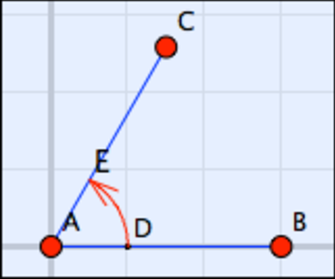
\includegraphics[width=3.5cm,bb=0 0 161 134]{Fig/setcolor.pdf} 

\begin{flushright}  \hyperlink{functionlist}{$\Rightarrow$関数一覧}\end{flushright}

\vspace{\baselineskip}
\hypertarget{deffun}{}
\item[関数]  Deffun(関数名 , 定義のリスト)
\item[機能]  関数を定義する
\item[説明]  関数定義は,CindyScript の関数定義 f(x):=式 でもできるが,Deffun()を使うことにより,Rでこの関数を利用することができる。目的に応じて使い分けるとよい。

式のリストには if文を用いた場合分けの関数式を記述することもできる。

\vspace{\baselineskip}
【例】
$f(x)=\dfrac{1}{x^2+1}$ を定義し,グラフを描く。

\begin{verbatim}
Deffun("f(x)",["regional(y)","y=1/(x^2+1)","y"]);
Plotdata("1","f(x)","x");
\end{verbatim}

\vspace{\baselineskip}
\hspace{20mm}\scalebox{0.9}{%%% /Users/Hannya/Desktop/KeTCindy/fig/deffun01.tex 
%%% Generator=template1basic.cdy 
{\unitlength=1cm%
\begin{picture}%
(6,3)(-3,-1)%
\special{pn 8}%
%
{%
\color[rgb]{0,0,0}%
\special{pa -1181   -39}\special{pa -1134   -42}\special{pa -1087   -46}\special{pa -1039   -49}%
\special{pa  -992   -54}\special{pa  -945   -58}\special{pa  -898   -64}\special{pa  -850   -69}%
\special{pa  -803   -76}\special{pa  -756   -84}\special{pa  -709   -93}\special{pa  -661  -103}%
\special{pa  -614  -115}\special{pa  -567  -128}\special{pa  -520  -144}\special{pa  -472  -161}%
\special{pa  -425  -182}\special{pa  -378  -205}\special{pa  -331  -231}\special{pa  -283  -259}%
\special{pa  -236  -289}\special{pa  -189  -320}\special{pa  -142  -349}\special{pa   -94  -372}%
\special{pa   -47  -388}\special{pa     0  -394}\special{pa    47  -388}\special{pa    94  -372}%
\special{pa   142  -349}\special{pa   189  -320}\special{pa   236  -289}\special{pa   283  -259}%
\special{pa   331  -231}\special{pa   378  -205}\special{pa   425  -182}\special{pa   472  -161}%
\special{pa   520  -144}\special{pa   567  -128}\special{pa   614  -115}\special{pa   661  -103}%
\special{pa   709   -93}\special{pa   756   -84}\special{pa   803   -76}\special{pa   850   -69}%
\special{pa   898   -64}\special{pa   945   -58}\special{pa   992   -54}\special{pa  1039   -49}%
\special{pa  1087   -46}\special{pa  1134   -42}\special{pa  1181   -39}%
\special{fp}%
}%
\special{pa -1181    -0}\special{pa  1181    -0}%
\special{fp}%
\special{pa     0   394}\special{pa     0  -787}%
\special{fp}%
\settowidth{\Width}{$x$}\setlength{\Width}{0\Width}%
\settoheight{\Height}{$x$}\settodepth{\Depth}{$x$}\setlength{\Height}{-0.5\Height}\setlength{\Depth}{0.5\Depth}\addtolength{\Height}{\Depth}%
\put(3.0500000,0.0000000){\hspace*{\Width}\raisebox{\Height}{$x$}}%
%
\settowidth{\Width}{$y$}\setlength{\Width}{-0.5\Width}%
\settoheight{\Height}{$y$}\settodepth{\Depth}{$y$}\setlength{\Height}{\Depth}%
\put(0.0000000,2.0500000){\hspace*{\Width}\raisebox{\Height}{$y$}}%
%
\settowidth{\Width}{O}\setlength{\Width}{-1\Width}%
\settoheight{\Height}{O}\settodepth{\Depth}{O}\setlength{\Height}{-\Height}%
\put(-0.0500000,-0.0500000){\hspace*{\Width}\raisebox{\Height}{O}}%
%
\end{picture}}%}

          
\vspace{\baselineskip}
  【例】$f(x)=\left\{\begin{array}{l}1  (x\geq 0)\\ -1   (x<0)\\ \end{array}\right.$     を定義してグラフを描く。

\begin{verbatim}
    Deffun("f(x)",["regional(y)","if(x>=0,y=1,y=-1)","y"]);
    Plotdata("1","f(x)","x",["Dis=1","Num=100"];
\end{verbatim}

\vspace{\baselineskip}
\hspace{20mm}\scalebox{0.9}{%%% /Users/Hannya/Desktop/KeTCindy/fig/deffun02.tex 
%%% Generator=template1basic.cdy 
{\unitlength=1cm%
\begin{picture}%
(6,3.14)(-3,-1.5)%
\special{pn 8}%
%
{%
\color[rgb]{0,0,0}%
\special{pa -1181   394}\special{pa -1157   394}\special{pa -1134   394}\special{pa -1110   394}%
\special{pa -1087   394}\special{pa -1063   394}\special{pa -1039   394}\special{pa -1016   394}%
\special{pa  -992   394}\special{pa  -969   394}\special{pa  -945   394}\special{pa  -921   394}%
\special{pa  -898   394}\special{pa  -874   394}\special{pa  -850   394}\special{pa  -827   394}%
\special{pa  -803   394}\special{pa  -780   394}\special{pa  -756   394}\special{pa  -732   394}%
\special{pa  -709   394}\special{pa  -685   394}\special{pa  -661   394}\special{pa  -638   394}%
\special{pa  -614   394}\special{pa  -591   394}\special{pa  -567   394}\special{pa  -543   394}%
\special{pa  -520   394}\special{pa  -496   394}\special{pa  -472   394}\special{pa  -449   394}%
\special{pa  -425   394}\special{pa  -402   394}\special{pa  -378   394}\special{pa  -354   394}%
\special{pa  -331   394}\special{pa  -307   394}\special{pa  -283   394}\special{pa  -260   394}%
\special{pa  -236   394}\special{pa  -213   394}\special{pa  -189   394}\special{pa  -165   394}%
\special{pa  -142   394}\special{pa  -118   394}\special{pa   -94   394}\special{pa   -71   394}%
\special{pa   -47   394}\special{pa   -24   394}%
\special{fp}%
\special{pa     0  -394}\special{pa    24  -394}\special{pa    47  -394}\special{pa    71  -394}%
\special{pa    94  -394}\special{pa   118  -394}\special{pa   142  -394}\special{pa   165  -394}%
\special{pa   189  -394}\special{pa   213  -394}\special{pa   236  -394}\special{pa   260  -394}%
\special{pa   283  -394}\special{pa   307  -394}\special{pa   331  -394}\special{pa   354  -394}%
\special{pa   378  -394}\special{pa   402  -394}\special{pa   425  -394}\special{pa   449  -394}%
\special{pa   472  -394}\special{pa   496  -394}\special{pa   520  -394}\special{pa   543  -394}%
\special{pa   567  -394}\special{pa   591  -394}\special{pa   614  -394}\special{pa   638  -394}%
\special{pa   661  -394}\special{pa   685  -394}\special{pa   709  -394}\special{pa   732  -394}%
\special{pa   756  -394}\special{pa   780  -394}\special{pa   803  -394}\special{pa   827  -394}%
\special{pa   850  -394}\special{pa   874  -394}\special{pa   898  -394}\special{pa   921  -394}%
\special{pa   945  -394}\special{pa   969  -394}\special{pa   992  -394}\special{pa  1016  -394}%
\special{pa  1039  -394}\special{pa  1063  -394}\special{pa  1087  -394}\special{pa  1110  -394}%
\special{pa  1134  -394}\special{pa  1157  -394}\special{pa  1181  -394}%
\special{fp}%
}%
\special{pa -1181    -0}\special{pa  1181    -0}%
\special{fp}%
\special{pa     0   591}\special{pa     0  -646}%
\special{fp}%
\settowidth{\Width}{$x$}\setlength{\Width}{0\Width}%
\settoheight{\Height}{$x$}\settodepth{\Depth}{$x$}\setlength{\Height}{-0.5\Height}\setlength{\Depth}{0.5\Depth}\addtolength{\Height}{\Depth}%
\put(3.0500000,0.0000000){\hspace*{\Width}\raisebox{\Height}{$x$}}%
%
\settowidth{\Width}{$y$}\setlength{\Width}{-0.5\Width}%
\settoheight{\Height}{$y$}\settodepth{\Depth}{$y$}\setlength{\Height}{\Depth}%
\put(0.0000000,1.6900000){\hspace*{\Width}\raisebox{\Height}{$y$}}%
%
\settowidth{\Width}{O}\setlength{\Width}{-1\Width}%
\settoheight{\Height}{O}\settodepth{\Depth}{O}\setlength{\Height}{-\Height}%
\put(-0.0500000,-0.0500000){\hspace*{\Width}\raisebox{\Height}{O}}%
%
\end{picture}}%}

  if 文はネストすることができる。
\begin{verbatim}
    Deffun("f(x)",["regional y","if(x>1,y=1,if(x>-1,y=x,y=-1))","y"]);
\end{verbatim}

\vspace{\baselineskip}
\hspace{20mm}\scalebox{0.9}{%%% /Users/Hannya/Desktop/KeTCindy/fig/deffun03.tex 
%%% Generator=template1basic.cdy 
{\unitlength=1cm%
\begin{picture}%
(6.03,3.23)(-3.03,-1.67)%
\special{pn 8}%
%
{%
\color[rgb]{0,0,0}%
\special{pa -1193   394}\special{pa -1145   394}\special{pa -1098   394}\special{pa -1050   394}%
\special{pa -1003   394}\special{pa  -956   394}\special{pa  -908   394}\special{pa  -861   394}%
\special{pa  -813   394}\special{pa  -766   394}\special{pa  -718   394}\special{pa  -671   394}%
\special{pa  -623   394}\special{pa  -576   394}\special{pa  -528   394}\special{pa  -481   394}%
\special{pa  -433   394}\special{pa  -386   386}\special{pa  -338   338}\special{pa  -291   291}%
\special{pa  -243   243}\special{pa  -196   196}\special{pa  -148   148}\special{pa  -101   101}%
\special{pa   -53    53}\special{pa    -6     6}\special{pa    42   -42}\special{pa    89   -89}%
\special{pa   137  -137}\special{pa   184  -184}\special{pa   231  -231}\special{pa   279  -279}%
\special{pa   326  -326}\special{pa   374  -374}\special{pa   421  -394}\special{pa   469  -394}%
\special{pa   516  -394}\special{pa   564  -394}\special{pa   611  -394}\special{pa   659  -394}%
\special{pa   706  -394}\special{pa   754  -394}\special{pa   801  -394}\special{pa   849  -394}%
\special{pa   896  -394}\special{pa   944  -394}\special{pa   991  -394}\special{pa  1039  -394}%
\special{pa  1086  -394}\special{pa  1134  -394}\special{pa  1181  -394}%
\special{fp}%
}%
\special{pa -1193    -0}\special{pa  1181    -0}%
\special{fp}%
\special{pa     0   657}\special{pa     0  -614}%
\special{fp}%
\settowidth{\Width}{$x$}\setlength{\Width}{0\Width}%
\settoheight{\Height}{$x$}\settodepth{\Depth}{$x$}\setlength{\Height}{-0.5\Height}\setlength{\Depth}{0.5\Depth}\addtolength{\Height}{\Depth}%
\put(3.0500000,0.0000000){\hspace*{\Width}\raisebox{\Height}{$x$}}%
%
\settowidth{\Width}{$y$}\setlength{\Width}{-0.5\Width}%
\settoheight{\Height}{$y$}\settodepth{\Depth}{$y$}\setlength{\Height}{\Depth}%
\put(0.0000000,1.6100000){\hspace*{\Width}\raisebox{\Height}{$y$}}%
%
\settowidth{\Width}{O}\setlength{\Width}{0\Width}%
\settoheight{\Height}{O}\settodepth{\Depth}{O}\setlength{\Height}{-\Height}%
\put(0.0500000,-0.0500000){\hspace*{\Width}\raisebox{\Height}{O}}%
%
\end{picture}}%}


\vspace{\baselineskip}
\hypertarget{defvar}{}
\item[関数]  Defvar(文字列)
\item[機能]  変数を定義する
\item[説明]  変数の定義をRと共有する。

【例】  \verb|Defvar("const=3");|

\vspace{\baselineskip}
  複数の変数を定義するときはリストにする。
  
【例】  \verb|Defvar([“a”,3,”b”,1]);|

\vspace{\baselineskip}
\hypertarget{fontsize}{}
\item[関数]  Fontsize(記号)
\item[機能]  フォントサイズを設定する
\item[説明]  次に Fontsize() を実行するまで有効\\
  記号は,"t" , "ss" , "f", "s" , "n" , "la",  "La", "LA", "h" , "H"\\

【例】作図ツールの「点を加える」で,A〜Gの点をとっておく。小さい方からいくつか表示する。
\begin{verbatim}
    Ptsize(2);
    Drawpoint([A,B,C,D,E,F,G]);
    Fontsize("t"); Letter([A,"s2","A"]);
    Fontsize("ss"); Letter([B,"s2","B"]);
    Fontsize("s"); Letter([C,"s2","C"]);
    Fontsize("la"); Letter([D,"s2","D"]);
    Fontsize("La"); Letter([E,"s2","E"]);
    Fontsize("h"); Letter([F,"s2","F"]);
    Fontsize("H"); Letter([G,"s2","G"]);
\end{verbatim}
%%% test.tex 2014-11-28 20:51
%%% test.sce 2014-11-28 20:51
{\unitlength=6mm%
\begin{picture}%
(  14.00000,   2.00000)(  -1.00000,   2.00000)%
\special{pn 8}%
%
\special{pa 6 -714}\special{pa 0 -717}\special{pa -6 -714}\special{pa -8 -709}\special{pa -6 -703}%
\special{pa 0 -701}\special{pa 6 -703}\special{pa 8 -709}\special{pa 6 -714}\special{sh 1}\special{fp}%
\special{pa 478 -714}\special{pa 472 -717}\special{pa 467 -714}\special{pa 465 -709}%
\special{pa 467 -703}\special{pa 472 -701}\special{pa 478 -703}\special{pa 480 -709}%
\special{pa 478 -714}\special{sh 1}\special{fp}%
\special{pa 950 -714}\special{pa 945 -717}\special{pa 939 -714}\special{pa 937 -709}%
\special{pa 939 -703}\special{pa 945 -701}\special{pa 950 -703}\special{pa 953 -709}%
\special{pa 950 -714}\special{sh 1}\special{fp}%
\special{pa 1423 -714}\special{pa 1417 -717}\special{pa 1412 -714}\special{pa 1409 -709}%
\special{pa 1412 -703}\special{pa 1417 -701}\special{pa 1423 -703}\special{pa 1425 -709}%
\special{pa 1423 -714}\special{sh 1}\special{fp}%
\special{pa 1895 -714}\special{pa 1890 -717}\special{pa 1884 -714}\special{pa 1882 -709}%
\special{pa 1884 -703}\special{pa 1890 -701}\special{pa 1895 -703}\special{pa 1898 -709}%
\special{pa 1895 -714}\special{sh 1}\special{fp}%
\special{pa 2368 -714}\special{pa 2362 -717}\special{pa 2357 -714}\special{pa 2354 -709}%
\special{pa 2357 -703}\special{pa 2362 -701}\special{pa 2368 -703}\special{pa 2370 -709}%
\special{pa 2368 -714}\special{sh 1}\special{fp}%
\special{pa 2840 -714}\special{pa 2835 -717}\special{pa 2829 -714}\special{pa 2827 -709}%
\special{pa 2829 -703}\special{pa 2835 -701}\special{pa 2840 -703}\special{pa 2843 -709}%
\special{pa 2840 -714}\special{sh 1}\special{fp}%
\tiny%
\settowidth{\Width}{A}\setlength{\Width}{-0.5\Width}%
\settoheight{\Height}{A}\settodepth{\Depth}{A}\setlength{\Height}{-\Height}%
\put(0.0000,2.8500){\hspace*{\Width}\raisebox{\Height}{A}}%
%
%
\scriptsize%
\settowidth{\Width}{B}\setlength{\Width}{-0.5\Width}%
\settoheight{\Height}{B}\settodepth{\Depth}{B}\setlength{\Height}{-\Height}%
\put(2.0000,2.8500){\hspace*{\Width}\raisebox{\Height}{B}}%
%
%
\small%
\settowidth{\Width}{C}\setlength{\Width}{-0.5\Width}%
\settoheight{\Height}{C}\settodepth{\Depth}{C}\setlength{\Height}{-\Height}%
\put(4.0000,2.8500){\hspace*{\Width}\raisebox{\Height}{C}}%
%
%
\large%
\settowidth{\Width}{D}\setlength{\Width}{-0.5\Width}%
\settoheight{\Height}{D}\settodepth{\Depth}{D}\setlength{\Height}{-\Height}%
\put(6.0000,2.8500){\hspace*{\Width}\raisebox{\Height}{D}}%
%
%
\Large%
\settowidth{\Width}{E}\setlength{\Width}{-0.5\Width}%
\settoheight{\Height}{E}\settodepth{\Depth}{E}\setlength{\Height}{-\Height}%
\put(8.0000,2.8500){\hspace*{\Width}\raisebox{\Height}{E}}%
%
%
\huge%
\settowidth{\Width}{F}\setlength{\Width}{-0.5\Width}%
\settoheight{\Height}{F}\settodepth{\Depth}{F}\setlength{\Height}{-\Height}%
\put(10.0000,2.8500){\hspace*{\Width}\raisebox{\Height}{F}}%
%
%
\Huge%
\settowidth{\Width}{G}\setlength{\Width}{-0.5\Width}%
\settoheight{\Height}{G}\settodepth{\Depth}{G}\setlength{\Height}{-\Height}%
\put(12.0000,2.8500){\hspace*{\Width}\raisebox{\Height}{G}}%
%
%
\end{picture}}%

\vspace{\baselineskip}
\hypertarget{setpt}{}
\hypertarget{ptsize}{}
\item[関数]  Ptsize(n) , Setpt(n)
\item[機能]  表示する点の大きさを設定する。
\item[説明]  Ptsize() と Setpt() は同じである。 初期設定は1

全体の点の大きさを設定する。点の大きさを個々に変えたい場合は,sizeオプションを用いる。

\vspace{\baselineskip}
【例】1から4までの点の大きさ

あらかじめ,Cinderellaの作図ツールで点A,B,C,Dを作図しておく。
\begin{verbatim}
    Pointdata("1",A,["Size=1"]);
    Pointdata("2",B,["Size=2"]);
    Pointdata("3",C,["Size=3"]);
    Pointdata("4",D,["Size=4"]);
\end{verbatim}
\hspace{10mm}%%% test.tex 2014-10-22 9:7
%%% test.sce 2014-10-22 9:7
{\unitlength=1cm%
\begin{picture}%
(   7.00000,   2.00000)(  -3.00000,  -1.00000)%
\special{pn 8}%
%
\special{pa 3 -3}\special{pa -3 -3}\special{pa -3 3}\special{pa 3 3}\special{pa 3 -3}%
\special{sh 1}\special{fp}%
\special{pa 399 -6}\special{pa 394 -8}\special{pa 388 -6}\special{pa 386 0}\special{pa 388 6}%
\special{pa 394 8}\special{pa 399 6}\special{pa 402 0}\special{pa 399 -6}\special{sh 1}\special{fp}%
\special{pa 796 -8}\special{pa 789 -12}\special{pa 782 -11}\special{pa 777 -5}\special{pa 776 2}%
\special{pa 779 8}\special{pa 786 12}\special{pa 793 11}\special{pa 798 5}\special{pa 799 -2}%
\special{pa 796 -8}\special{sh 1}\special{fp}%
\special{pa 1192 -11}\special{pa 1185 -15}\special{pa 1177 -15}\special{pa 1170 -11}%
\special{pa 1166 -4}\special{pa 1166 4}\special{pa 1170 11}\special{pa 1177 15}\special{pa 1185 15}%
\special{pa 1192 11}\special{pa 1196 4}\special{pa 1196 -4}\special{pa 1192 -11}\special{sh 1}\special{fp}%
\settowidth{\Width}{Pointsize}\setlength{\Width}{-0.5\Width}%
\settoheight{\Height}{Pointsize}\settodepth{\Depth}{Pointsize}\setlength{\Height}{\Depth}%
\put(-1.4400,0.1500){\hspace*{\Width}\raisebox{\Height}{Pointsize}}%
%
%
\settowidth{\Width}{1}\setlength{\Width}{-0.5\Width}%
\settoheight{\Height}{1}\settodepth{\Depth}{1}\setlength{\Height}{\Depth}%
\put(0.0000,0.1500){\hspace*{\Width}\raisebox{\Height}{1}}%
%
%
\settowidth{\Width}{2}\setlength{\Width}{-0.5\Width}%
\settoheight{\Height}{2}\settodepth{\Depth}{2}\setlength{\Height}{\Depth}%
\put(1.0000,0.1500){\hspace*{\Width}\raisebox{\Height}{2}}%
%
%
\settowidth{\Width}{3}\setlength{\Width}{-0.5\Width}%
\settoheight{\Height}{3}\settodepth{\Depth}{3}\setlength{\Height}{\Depth}%
\put(2.0000,0.1500){\hspace*{\Width}\raisebox{\Height}{3}}%
%
%
\settowidth{\Width}{4}\setlength{\Width}{-0.5\Width}%
\settoheight{\Height}{4}\settodepth{\Depth}{4}\setlength{\Height}{\Depth}%
\put(3.0000,0.1500){\hspace*{\Width}\raisebox{\Height}{4}}%
%
%
\end{picture}}%

\hypertarget{setmarklen}{}
\item[関数]  Setmarklen(数)  
\item[機能]  座標軸の目盛の長さを設定する
\item[説明]   \hyperlink{htickmark}{Htickmark()} , Vtickmark() で座標軸に目盛を入れるとき,その長さを設定する。 

\vspace{\baselineskip}
\hypertarget{setorigin}{}
\item[関数]  Setorigin(座標)      
\item[機能]  描画する座標軸の原点を設定(移動)する。座標系は変化しない。
\item[説明]  描画する座標軸の原点を引数の座標とする。座標は点の識別名でもよい。

\vspace{\baselineskip}
【例】原点を (3,2) として座標軸を描く。

\hspace{10mm}  \verb|Setorigin([3,2]);|

原点を点Aの位置にして座標軸を描く。

\hspace{10mm}  \verb|Setorigin(A);|  

\vspace{\baselineskip}
  【例】原点は(3,2)に移動するが,スクリプトではもとの座標系を使う。
\begin{verbatim}
      Setorigin([3,2]);
      Listplot([A,B,C,A]);
      Ptsize(3);
      Drawpoint([1,1]);
      Letter([[1,1],"s2","P"]);
\end{verbatim}
  左が実行時のCinderellaの画面,右が\TeX の結果。\\

\hspace{10mm} 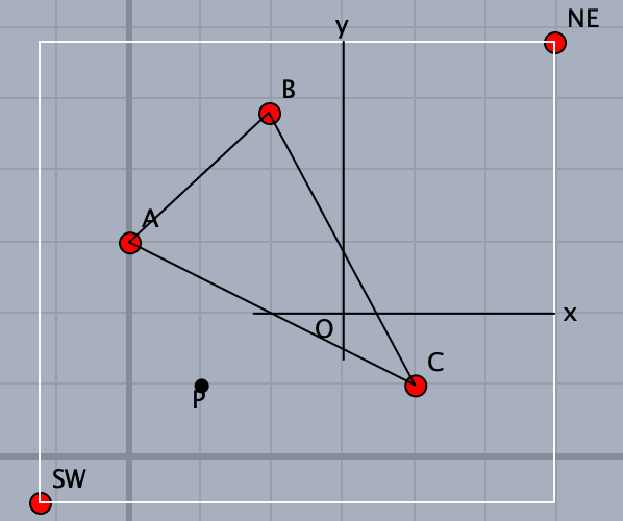
\includegraphics[bb=0 0 227 205 , width=4cm]{Fig/setorigin.pdf}     %%% test.tex 2014-11-28 22:0
%%% test.sce 2014-11-28 22:0
{\unitlength=6mm%
\begin{picture}%
(   6.00000,   6.00000)(  -1.00000,   0.00000)%
\special{pn 8}%
%
\special{pa 245 -245}\special{pa 238 -248}\special{pa 231 -247}\special{pa 226 -242}%
\special{pa 225 -234}\special{pa 228 -228}\special{pa 234 -225}\special{pa 242 -226}%
\special{pa 247 -231}\special{pa 248 -238}\special{pa 245 -245}\special{sh 1}\special{fp}%
\settowidth{\Width}{P}\setlength{\Width}{-0.5\Width}%
\settoheight{\Height}{P}\settodepth{\Depth}{P}\setlength{\Height}{-\Height}%
\put(1.0000,0.8500){\hspace*{\Width}\raisebox{\Height}{P}}%
%
%
\special{pa 0 -709}\special{pa 472 -1181}\special{pa 945 -236}\special{pa 0 -709}%
\special{fp}%
\special{pa -236 -472}\special{pa 1181 -472}%
\special{fp}%
\special{pa 709 0}\special{pa 709 -1417}%
\special{fp}%
\settowidth{\Width}{$x$}\setlength{\Width}{0\Width}%
\settoheight{\Height}{$x$}\settodepth{\Depth}{$x$}\setlength{\Height}{-0.5\Height}\setlength{\Depth}{0.5\Depth}\addtolength{\Height}{\Depth}%
\put(5.0500,2.0000){\hspace*{\Width}\raisebox{\Height}{$x$}}%
%
%
\settowidth{\Width}{$y$}\setlength{\Width}{-0.5\Width}%
\settoheight{\Height}{$y$}\settodepth{\Depth}{$y$}\setlength{\Height}{\Depth}%
\put(3.0000,6.0500){\hspace*{\Width}\raisebox{\Height}{$y$}}%
%
%
\settowidth{\Width}{O}\setlength{\Width}{-1\Width}%
\settoheight{\Height}{O}\settodepth{\Depth}{O}\setlength{\Height}{-\Height}%
\put(2.9500,1.9500){\hspace*{\Width}\raisebox{\Height}{O}}%
%
%
\end{picture}}% 

\vspace{\baselineskip}
\hypertarget{setpen}{}
\item[関数]  Setpen(数)      
\item[機能]  線の太さの初期値を設定する

\verb|Listplot()| などの描画関数のオプション \verb|dr| で,個々の太さは指定できる。

\vspace{\baselineskip}
\hypertarget{setscaling}{}
\item[関数]  Setscaling(倍率)
\item[機能]  縦方向の倍率を設定する。倍率は実数またはリスト。実数の場合は縦方向,リストの場合は[横方向,縦方向]の指定となる。
\item[説明]  2次関数の応用問題などでは,グラフが縦に大きくなる場合があり,$y$軸方向のスケーリングを変えたいことがよくある。次のスクリプトは,$f(x)=-x^2+10x$ のグラフを縦軸方向を半分にして描くものである。

\begin{layer}{150}{0}
\putnotese{80}{5}{%%% test.tex 2014-10-22 10:38
%%% test.sce 2014-10-22 10:38
{\unitlength=5mm%
\begin{picture}%
(   7.00000,   8.00000)(  -1.00000,  -1.00000)%
\special{pn 8}%
%
\special{pn 8}%
\special{pa -4 -1230}\special{pa 4 -1230}\special{fp}\special{pa 34 -1230}\special{pa 42 -1230}\special{fp}%
\special{pa 72 -1230}\special{pa 80 -1230}\special{fp}\special{pa 110 -1230}\special{pa 118 -1230}\special{fp}%
\special{pa 147 -1230}\special{pa 155 -1230}\special{fp}\special{pa 185 -1230}\special{pa 193 -1230}\special{fp}%
\special{pa 223 -1230}\special{pa 231 -1230}\special{fp}\special{pa 261 -1230}\special{pa 269 -1230}\special{fp}%
\special{pa 299 -1230}\special{pa 307 -1230}\special{fp}\special{pa 337 -1230}\special{pa 345 -1230}\special{fp}%
\special{pa 375 -1230}\special{pa 383 -1230}\special{fp}\special{pa 412 -1230}\special{pa 420 -1230}\special{fp}%
\special{pa 450 -1230}\special{pa 458 -1230}\special{fp}\special{pa 488 -1230}\special{pa 496 -1230}\special{fp}%
\special{pn 8}%
\special{pn 8}%
\special{pa 492 4}\special{pa 492 -4}\special{fp}\special{pa 492 -36}\special{pa 492 -44}\special{fp}%
\special{pa 492 -75}\special{pa 492 -83}\special{fp}\special{pa 492 -115}\special{pa 492 -123}\special{fp}%
\special{pa 492 -155}\special{pa 492 -163}\special{fp}\special{pa 492 -194}\special{pa 492 -202}\special{fp}%
\special{pa 492 -234}\special{pa 492 -242}\special{fp}\special{pa 492 -274}\special{pa 492 -282}\special{fp}%
\special{pa 492 -314}\special{pa 492 -322}\special{fp}\special{pa 492 -353}\special{pa 492 -361}\special{fp}%
\special{pa 492 -393}\special{pa 492 -401}\special{fp}\special{pa 492 -433}\special{pa 492 -441}\special{fp}%
\special{pa 492 -472}\special{pa 492 -480}\special{fp}\special{pa 492 -512}\special{pa 492 -520}\special{fp}%
\special{pa 492 -552}\special{pa 492 -560}\special{fp}\special{pa 492 -591}\special{pa 492 -599}\special{fp}%
\special{pa 492 -631}\special{pa 492 -639}\special{fp}\special{pa 492 -671}\special{pa 492 -679}\special{fp}%
\special{pa 492 -710}\special{pa 492 -718}\special{fp}\special{pa 492 -750}\special{pa 492 -758}\special{fp}%
\special{pa 492 -790}\special{pa 492 -798}\special{fp}\special{pa 492 -829}\special{pa 492 -837}\special{fp}%
\special{pa 492 -869}\special{pa 492 -877}\special{fp}\special{pa 492 -909}\special{pa 492 -917}\special{fp}%
\special{pa 492 -949}\special{pa 492 -957}\special{fp}\special{pa 492 -988}\special{pa 492 -996}\special{fp}%
\special{pa 492 -1028}\special{pa 492 -1036}\special{fp}\special{pa 492 -1068}\special{pa 492 -1076}\special{fp}%
\special{pa 492 -1107}\special{pa 492 -1115}\special{fp}\special{pa 492 -1147}\special{pa 492 -1155}\special{fp}%
\special{pa 492 -1187}\special{pa 492 -1195}\special{fp}\special{pa 492 -1226}\special{pa 492 -1234}\special{fp}%
\special{pn 8}%
\settowidth{\Width}{5}\setlength{\Width}{-1\Width}%
\settoheight{\Height}{5}\settodepth{\Depth}{5}\setlength{\Height}{-\Height}%
\put(4.9500,-0.1500){\hspace*{\Width}\raisebox{\Height}{5}}%
%
%
\settowidth{\Width}{$\frac{25}{2}$}\setlength{\Width}{-1\Width}%
\settoheight{\Height}{$\frac{25}{2}$}\settodepth{\Depth}{$\frac{25}{2}$}\setlength{\Height}{-0.5\Height}\setlength{\Depth}{0.5\Depth}\addtolength{\Height}{\Depth}%
\put(-0.1500,6.2500){\hspace*{\Width}\raisebox{\Height}{$\frac{25}{2}$}}%
%
%
\settowidth{\Width}{$\frac{5}{2}$}\setlength{\Width}{-0.5\Width}%
\settoheight{\Height}{$\frac{5}{2}$}\settodepth{\Depth}{$\frac{5}{2}$}\setlength{\Height}{-\Height}%
\put(2.5000,-0.2500){\hspace*{\Width}\raisebox{\Height}{$\frac{5}{2}$}}%
%
%
\special{pa -38 197}\special{pa -28 145}\special{pa 0 0}\special{pa 28 -137}\special{pa 56 -265}%
\special{pa 84 -386}\special{pa 112 -498}\special{pa 141 -603}\special{pa 169 -699}%
\special{pa 197 -787}\special{pa 225 -868}\special{pa 253 -940}\special{pa 281 -1004}%
\special{pa 309 -1061}\special{pa 337 -1109}\special{pa 366 -1149}\special{pa 394 -1181}%
\special{pa 422 -1205}\special{pa 450 -1221}\special{pa 478 -1229}\special{pa 506 -1229}%
\special{pa 534 -1221}\special{pa 562 -1205}\special{pa 591 -1181}\special{pa 619 -1149}%
\special{pa 647 -1109}\special{pa 675 -1061}\special{pa 703 -1004}\special{pa 731 -940}%
\special{pa 759 -868}\special{pa 787 -787}\special{pa 816 -699}\special{pa 844 -603}%
\special{pa 872 -498}\special{pa 900 -386}\special{pa 928 -265}\special{pa 956 -137}%
\special{pa 984 0}\special{pa 1012 145}\special{pa 1022 197}%
\special{fp}%
\special{pa -197 0}\special{pa 1181 0}%
\special{fp}%
\special{pa 0 197}\special{pa 0 -1378}%
\special{fp}%
\settowidth{\Width}{$x$}\setlength{\Width}{0\Width}%
\settoheight{\Height}{$x$}\settodepth{\Depth}{$x$}\setlength{\Height}{-0.5\Height}\setlength{\Depth}{0.5\Depth}\addtolength{\Height}{\Depth}%
\put(6.0500,0.0000){\hspace*{\Width}\raisebox{\Height}{$x$}}%
%
%
\settowidth{\Width}{$y$}\setlength{\Width}{-0.5\Width}%
\settoheight{\Height}{$y$}\settodepth{\Depth}{$y$}\setlength{\Height}{\Depth}%
\put(0.0000,7.0500){\hspace*{\Width}\raisebox{\Height}{$y$}}%
%
%
\settowidth{\Width}{O}\setlength{\Width}{-1\Width}%
\settoheight{\Height}{O}\settodepth{\Depth}{O}\setlength{\Height}{-\Height}%
\put(-0.0500,-0.0500){\hspace*{\Width}\raisebox{\Height}{O}}%
%
%
\end{picture}}%}
\end{layer}
\begin{verbatim}
  Setscaling(0.5);
  A.xy=[0,25/4];
  B.xy=[5/2,25/4];
  C.xy=[5/2,0];
  Listplot([A,B],["do"]);
  Listplot([C,B],["do"]);
  Plotdata("1","-2*x^2+10*x","x");
  Letter([[5,0],"s2w","5",[0,25/2],"w2",
      "$\frac{25}{2}$",C,"s4","$\frac{5}{2}$"]);
\end{verbatim}
  ここで,点A,Bの座標が
\begin{verbatim}
    A.xy=[0,25/4];
    B.xy=[5/2,25/4];
\end{verbatim}
となっていることに注意されたい。$y$座標をあらかじめ半分にしている。すなわち,Cinderellaで作図した幾何要素に対してはSetscalingは無効である。これは,Putpoint関数を用いて点の位置を決めても同じである。

たとえば,次のスクリプトでは,Cinderellaの画面上では2本の線分が点Bでつながるが,書き出された\TeX の図では離れてしまう。
\begin{verbatim}
    Setscaling(0.5);
    Putpoint("A",[0,2]);
    Putpoint("B",[2,2]);
    Listplot([A,B]);
    Listplot("1",[[0,0],[2,2]]);
\end{verbatim}

\begin{flushright}  \hyperlink{functionlist}{$\Rightarrow$関数一覧}\end{flushright}

\vspace{\baselineskip}
\hypertarget{setunitlen}{}
\item[関数]  Setunitlen(文字列)
\item[機能]  単位長を設定する。 初期設定は 1cm。

この関数は,スクリプトの初めの方に書くのがよい。
  
【例】Setunitlen("8mm")
  
\vspace{\baselineskip}
\hypertarget{setwindow}{}
\item[関数]  Setwindow()
\item[機能]  出力する描画領域を設定する
\item[説明]  出力する描画領域は,通常は2点SWとNEを対角とする矩形領域である。

この2点をドラッグすることによりビジュアルに描画領域を決められる。

しかし,これとは別に出力範囲を設定したい場合にこの関数を用いる。

また,表を作成したときは,表の範囲が出力範囲として優先される(Tabledata()を実行したとき)ので,表外に図を描いた場合は,最後にこの関数で出力範囲を指定して書き出す。

\begin{flushright}  \hyperlink{functionlist}{$\Rightarrow$関数一覧}\end{flushright}

\end{description}

\newpage
%=========== 描画 ======================
\subsection{描画}
\subsubsection{書式とオプション}

描画関数は曲線などを作図する関数である。

基本的な書式は

\hspace{20mm} 関数名(name , 点リストなど , options);

である。

nameは,プロットデータの名称で,関数ごとに決められた頭部のあとに付けられる。たとえば,線分を描く Listplot() でできるプロットデータは,頭部が"sg"であり,nameを"1"とすれば,"sg1" という名称のプロットデータができる。name指定は不要の場合もあり,その場合は \ketcindy が自動的に名称を作成する。

点リストなどには,点の座標,点の識別名,複数の点のリスト,複数の点を示す文字列などがあり,関数によって異なる。点はCinderellaで作図した幾何要素の点を利用できる。

optionsは,線種・表示する文字列・解像度・出力の有無などを指定するオプション群。

 線種はつぎの4通り。 初期設定は実線。

\begin{tabbing}
1234\=5678901234567\=\kill
  \>    "dr, n"     \>太さnの実線で描く。\\
  \>    "da,m,n"  \>破線を描く。\\
  \>                \> mは破線の長さ,nは破線の間隔  (m,nは省略可)\\
  \>                 \>m,n オプションはCinderellaの描画面には反映されない。\\
  \>    "id,m,n"   \>ギャップからはじまる破線を描く。\\
  \>    "do,m,n"  \>点線で描く。\\
  \>                \>mは点の間隔,nは太さ  (m,nは省略可)
\end{tabbing}

描画色指定は,RGBまたはCMYKのリストで指定するか,色名を用いる。

\hspace{10mm}【例】\verb|"Color=[0,0.7,0]"| で暗い緑になる。

出力の有無は
\begin{tabbing}
  1234\=567890123\=\kill
 \>    "notex"  \>Cinderella画面上の図形を出力しない\\
 \>    "nodisp" \>Cinderella画面上にも出力しない
 \end{tabbing}
 
 "nodisp"は画面上にも,Rへのデータにも出力されないが,プロットデータは作成されるので,プロットデータだけを利用したい場合に有効である。
 
\hspace{10mm}【例】  \verb|pdata=Circledata([A,B],["nodisp"]);|

として,後にプロットデータ pdata を利用する。

その他,次のようなオプションがある。
\begin{tabbing}
  1234\=567890123\=\kill
 \>    "Size=n"  \>点の大きさ,線の太さの指定\\
 \>    "Num=n"  \>曲線の場合の分割数(プロットデータの個数+1)\\
\end{tabbing}

%=========== 点・直線 ======================
\subsubsection{点・線分・直線}
\begin{description}

\vspace{\baselineskip}
\hypertarget{pointdata}{}
\item[関数]  Pointdata(name , 点リスト , options)
\item[機能]  点のデータを作成する。
\item[説明]  与えられた座標の点データを作成する。オプションは"Size=","Color="。

\vspace{\baselineskip}
【例】

(1) 座標指定で2つの点データを作る。

\hspace{10mm} \verb|Pointdata("1",[[1,2],[-2,3]]);|

(2) 作図した点A,Bについて,点データを作る。

\hspace{10mm} \verb|Pointdata("1",[A,B]);|
      
\hspace{5mm}A,Bが作図されていない場合は作成されない。

\hspace{5mm}Cinderellaの描画面上では既存の点A,Bに黒の点が重なって表示される。

(3) Aの位置に大きさ4で点を作る。

\hspace{10mm} \verb|Pointdata("1",A,["size=4"]);|
      
(4) 点データを作り,TeXにオプション0(白抜き)で描く

\hspace{10mm}  \verb|Pointdata("1",[A,B],[0]);|
      
(5) 点データを作るが,TeXには出力しない

\hspace{10mm}  \verb|Pointdata("1",[[3,4],[5,6]],["notex"]);|

(6)  点データを作るが,TeXには出力せず画面上にも表示しない。
        
\hspace{10mm} \verb|Pointdata("1",[[3,4],[5,6]],["nodisp"]);|

(7) 節点を明示した木を描く
\begin{verbatim}
  Ptsize(3); 
  Pointdata("1",[[1,2],[3,4],[5,2]]); 
  Listplot("1",[[0,0],[1,2],[3,4],[5,2],[4,0]]); 
  Listplot("2",[[1,2],[2,0]]); 
  Listplot("3",[[5,2],[6,0]]);
\end{verbatim}
 
 \begin{center} %%% test.tex 2014-11-28 14:29
%%% test.sce 2014-11-28 14:29
{\unitlength=6mm%
\begin{picture}%
(  14.00000,   4.00000)(   0.00000,   1.00000)%
\special{pn 8}%
%
\special{pa 245 -481}\special{pa 238 -484}\special{pa 231 -483}\special{pa 226 -478}%
\special{pa 225 -471}\special{pa 228 -464}\special{pa 234 -461}\special{pa 242 -462}%
\special{pa 247 -467}\special{pa 248 -474}\special{pa 245 -481}\special{sh 1}\special{fp}%
\special{pa 717 -953}\special{pa 711 -957}\special{pa 703 -955}\special{pa 698 -950}%
\special{pa 697 -943}\special{pa 700 -937}\special{pa 707 -933}\special{pa 714 -934}%
\special{pa 719 -940}\special{pa 720 -947}\special{pa 717 -953}\special{sh 1}\special{fp}%
\special{pa 1426 -481}\special{pa 1419 -484}\special{pa 1412 -483}\special{pa 1407 -478}%
\special{pa 1406 -471}\special{pa 1409 -464}\special{pa 1415 -461}\special{pa 1423 -462}%
\special{pa 1428 -467}\special{pa 1429 -474}\special{pa 1426 -481}\special{sh 1}\special{fp}%
\special{pa 236 -472}\special{pa 709 -945}\special{pa 1417 -472}%
\special{fp}%
\special{pa 1890 -472}\special{pa 2362 -945}\special{pa 3071 -472}%
\special{fp}%
\end{picture}}% \end{center}

注) 幾何点の有無など,付録の「\hyperlink{mkpttable}{点の作図についての比較表}」を参照のこと。

%\begin{flushright}  \hyperlink{functionlist}{$\Rightarrow$関数一覧}\end{flushright}

\vspace{\baselineskip}
\hypertarget{drwpt}{}
\item[関数]  Drwpt(点,option), Drawpoint(点,options)
\item[機能]  点を表示する
\item[説明]  座標または幾何点の識別名を与えて点を表示する。これだけではCinderellaの描画面には描かれないので,描画面にも表示するにはCinderellaの作図ツールで作図するか,Pointdata() または Putpoint() を用いる。

複数の点の場合は座標または識別名はリストで与える。

optionに数字 0 を入れると,白抜きで表示する。なお白抜きの場合は,Ptsize()で点の大きさを少し大きめにとるとよい。

可読性を高めるときはDrawpointを推奨する。

\vspace{\baselineskip}
【例】座標(1,1)と(4,3)に点を表示する。Cinderellaの描画面には描かれない。

\hspace{10mm} \verb|Drwpt([[1,1],[4,3]]);|

\vspace{\baselineskip}
【例】Cinderellaで点A,B,Cを作図しておき,\TeX で表示する。

\hspace{10mm} \verb|Drwpt([A,B,C]); |

\vspace{\baselineskip}
【例】線分ABの右端(B)を白抜きで表示する

\begin{layer}{150}{0}
\putnotese{50}{8}{  %%% test.tex 2014-10-21 18:7
%%% test.sce 2014-10-21 18:7
{\unitlength=1cm%
\begin{picture}%
(   5.00000,   2.00000)(  -1.00000,  -1.00000)%
\special{pn 8}%
%
\special{pa 1198 -17}\special{pa 1190 -22}\special{pa 1180 -24}\special{pa 1170 -21}%
\special{pa 1163 -15}\special{pa 1158 -6}\special{pa 1158 4}\special{pa 1161 13}\special{pa 1168 20}%
\special{pa 1177 23}\special{pa 1187 23}\special{pa 1196 18}\special{pa 1202 11}\special{pa 1205 1}%
\special{pa 1203 -8}\special{pa 1198 -17}\special{sh 0}\special{fp}%
\special{pa 0 0}\special{pa 1181 0}%
\special{fp}%
\end{picture}}%}
\end{layer}
\begin{verbatim}
      Ptsize(5);
      Listplot([A,B]);
      Drawpoint(B,0);
\end{verbatim}

※  Drawpoint([A,B],0);  とすれば,両端が白抜きになる。

\vspace{\baselineskip}
{\bf 点の表示方法}

点を表示する関数はいくつかある。Cinderellaの描画面上に単に点を表示するもの,幾何点を作るもの,TeXに出力するためのもの,と少しずつ意味が異なる。

付録の「\hyperlink{mkpttable}{点の作図についての比較表}」を参照のこと。

\begin{flushright}  \hyperlink{functionlist}{$\Rightarrow$関数一覧}\end{flushright}

\vspace{\baselineskip}
\hypertarget{putpoint}{}
\item[関数]  Putpoint(点名 , 座標1 ,座標2 )
\item[機能]  点を作る
\item[説明]  識別名が点名の点を,既存でなければ座標1に作る。既存ならば座標2に移動する。Texには出力されない。

\vspace{\baselineskip}
【例】点Aを作る。

(1,1) に固定点Aを作る。 この点は動かすことができない。

\hspace{10mm}   \verb|Putpoint("A",[1,1]);|
 
    (1,1)に自由点を作るには次のようにする。
    
\hspace{10mm}  \verb|Putpoint("A",[1,1],[A.x,A.y]);|
 
    この点は座標2の効果により,自由点となり,ドラッグして動かすことができる。

\vspace{\baselineskip}
注)点名は半角アルファベットとする。数字や漢字でもCinderellaでは点ができるが,Rでエラーとなる。

\vspace{\baselineskip}
\hypertarget{putintersect}{}
\item[関数]  Putintersect(点名 , PD1 , PD2 , [No] )
\item[機能]  2曲線の交点を作る
\item[説明]  PD1,PD2は2曲線のプロットデータ名。作成される点は幾何点。

描画範囲に交点が1つだけのとき,第4引数がなくても交点が作られる。

描画範囲に2つ以上の交点がある場合,第4引数を省略するとコンソールに交点の座標のリストと,「Choose point number 」というガイドが表示される。そこで,引数のNoとして,その番号を指定すると,その点が作られる。この関数で作成されるのは幾何点だけなので,\TeX の図に点として明示するためにはPointdata()で書き出す。

次の例は,3次曲線と直線の交点を3つとも取ったものである。

\begin{layer}{150}{0}
\putnotese{80}{5}{  %%% fig.tex 2015-8-3 21:32
%%% fig.sce 2015-8-3 21:32
{\unitlength=4mm%
\begin{picture}%
(   7.06000,   7.34000)(  -3.06000,  -3.34000)%
\special{pn 8}%
%
\special{pa -367 526}\special{pa -365 495}\special{pa -359 429}\special{pa -353 366}%
\special{pa -348 305}\special{pa -342 247}\special{pa -337 192}\special{pa -331 139}%
\special{pa -325 88}\special{pa -320 40}\special{pa -314 -5}\special{pa -309 -49}%
\special{pa -303 -90}\special{pa -298 -128}\special{pa -292 -165}\special{pa -286 -199}%
\special{pa -281 -231}\special{pa -275 -261}\special{pa -270 -288}\special{pa -264 -314}%
\special{pa -258 -338}\special{pa -253 -360}\special{pa -247 -380}\special{pa -242 -398}%
\special{pa -236 -414}\special{pa -230 -428}\special{pa -225 -441}\special{pa -219 -452}%
\special{pa -214 -461}\special{pa -208 -469}\special{pa -203 -475}\special{pa -197 -480}%
\special{pa -191 -483}\special{pa -186 -485}\special{pa -180 -485}\special{pa -175 -484}%
\special{pa -169 -481}\special{pa -163 -478}\special{pa -158 -473}\special{pa -152 -467}%
\special{pa -147 -459}\special{pa -141 -451}\special{pa -135 -442}\special{pa -130 -431}%
\special{pa -124 -420}\special{pa -119 -407}\special{pa -113 -394}\special{pa -108 -380}%
\special{pa -102 -365}\special{pa -96 -349}\special{pa -91 -333}\special{pa -85 -316}%
\special{pa -80 -298}\special{pa -74 -280}\special{pa -68 -261}\special{pa -63 -241}%
\special{pa -57 -222}\special{pa -52 -201}\special{pa -46 -180}\special{pa -41 -159}%
\special{pa -35 -138}\special{pa -29 -116}\special{pa -24 -94}\special{pa -18 -72}%
\special{pa -13 -50}\special{pa -7 -28}\special{pa -1 -6}\special{pa 4 17}\special{pa 10 39}%
\special{pa 15 61}\special{pa 21 83}\special{pa 27 105}\special{pa 32 127}\special{pa 38 149}%
\special{pa 43 170}\special{pa 49 191}\special{pa 54 211}\special{pa 60 231}\special{pa 66 251}%
\special{pa 71 270}\special{pa 77 289}\special{pa 82 307}\special{pa 88 324}\special{pa 94 341}%
\special{pa 99 357}\special{pa 105 373}\special{pa 110 387}\special{pa 116 401}\special{pa 122 414}%
\special{pa 127 426}\special{pa 133 437}\special{pa 138 446}\special{pa 144 455}\special{pa 149 463}%
\special{pa 155 470}\special{pa 161 475}\special{pa 166 480}\special{pa 172 483}\special{pa 177 484}%
\special{pa 183 485}\special{pa 189 484}\special{pa 194 482}\special{pa 200 478}\special{pa 205 472}%
\special{pa 211 465}\special{pa 216 457}\special{pa 222 447}\special{pa 228 435}\special{pa 233 421}%
\special{pa 239 406}\special{pa 244 389}\special{pa 250 370}\special{pa 256 349}\special{pa 261 326}%
\special{pa 267 302}\special{pa 272 275}\special{pa 278 246}\special{pa 284 215}\special{pa 289 182}%
\special{pa 295 147}\special{pa 300 109}\special{pa 306 70}\special{pa 311 28}\special{pa 317 -17}%
\special{pa 323 -64}\special{pa 328 -113}\special{pa 334 -165}\special{pa 339 -219}%
\special{pa 345 -276}\special{pa 351 -335}\special{pa 356 -397}\special{pa 362 -462}%
\special{pa 367 -529}\special{pa 373 -600}\special{pa 375 -630}%
\special{fp}%
\special{pa -482 83}\special{pa -459 72}\special{pa -437 61}\special{pa -414 49}\special{pa -391 38}%
\special{pa -368 27}\special{pa -346 15}\special{pa -323 4}\special{pa -300 -7}\special{pa -278 -19}%
\special{pa -255 -30}\special{pa -232 -41}\special{pa -210 -53}\special{pa -187 -64}%
\special{pa -164 -75}\special{pa -142 -87}\special{pa -119 -98}\special{pa -96 -109}%
\special{pa -73 -121}\special{pa -51 -132}\special{pa -28 -143}\special{pa -5 -155}%
\special{pa 17 -166}\special{pa 40 -177}\special{pa 63 -189}\special{pa 85 -200}\special{pa 108 -212}%
\special{pa 131 -223}\special{pa 153 -234}\special{pa 176 -246}\special{pa 199 -257}%
\special{pa 222 -268}\special{pa 244 -280}\special{pa 267 -291}\special{pa 290 -302}%
\special{pa 312 -314}\special{pa 335 -325}\special{pa 358 -336}\special{pa 380 -348}%
\special{pa 403 -359}\special{pa 426 -370}\special{pa 448 -382}\special{pa 471 -393}%
\special{pa 494 -404}\special{pa 516 -416}\special{pa 539 -427}\special{pa 562 -438}%
\special{pa 585 -450}\special{pa 607 -461}\special{pa 630 -472}%
\special{fp}%
\special{pa -304 -11}\special{pa -311 -15}\special{pa -319 -15}\special{pa -326 -11}%
\special{pa -330 -4}\special{pa -330 4}\special{pa -326 11}\special{pa -319 15}\special{pa -311 15}%
\special{pa -304 11}\special{pa -300 4}\special{pa -300 -4}\special{pa -304 -11}\special{sh 1}\special{fp}%
\special{pa -24 -151}\special{pa -31 -155}\special{pa -39 -155}\special{pa -47 -151}%
\special{pa -51 -144}\special{pa -51 -136}\special{pa -47 -129}\special{pa -39 -125}%
\special{pa -31 -125}\special{pa -24 -129}\special{pa -20 -136}\special{pa -20 -144}%
\special{pa -24 -151}\special{sh 1}\special{fp}%
\special{pa 361 -344}\special{pa 354 -348}\special{pa 346 -348}\special{pa 339 -344}%
\special{pa 335 -337}\special{pa 335 -329}\special{pa 339 -322}\special{pa 346 -317}%
\special{pa 354 -317}\special{pa 361 -322}\special{pa 366 -329}\special{pa 366 -337}%
\special{pa 361 -344}\special{sh 1}\special{fp}%
\special{pn 8}%
\special{pa -482 0}\special{pa 630 0}%
\special{fp}%
\special{pn 8}%
\special{pa 555 24}\special{pa 630 0}\special{pa 555 -24}\special{pa 555 0}\special{pa 555 24}%
\special{sh 1}\special{ip}%
\special{pn 8}%
\special{pa 555 24}\special{pa 630 0}\special{pa 555 -24}\special{pa 555 0}\special{pa 555 24}%
\special{fp}%
\special{pn 8}%
\special{pn 8}%
\special{pa 0 526}\special{pa 0 -630}%
\special{fp}%
\special{pn 8}%
\special{pa 24 -555}\special{pa 0 -630}\special{pa -24 -555}\special{pa 0 -555}\special{pa 24 -555}%
\special{sh 1}\special{ip}%
\special{pn 8}%
\special{pa 24 -555}\special{pa 0 -630}\special{pa -24 -555}\special{pa 0 -555}\special{pa 24 -555}%
\special{fp}%
\special{pn 8}%
\settowidth{\Width}{$x$}\setlength{\Width}{0\Width}%
\settoheight{\Height}{$x$}\settodepth{\Depth}{$x$}\setlength{\Height}{-0.5\Height}\setlength{\Depth}{0.5\Depth}\addtolength{\Height}{\Depth}%
\put(4.0500,0.0000){\hspace*{\Width}\raisebox{\Height}{$x$}}%
%
%
\settowidth{\Width}{$y$}\setlength{\Width}{-0.5\Width}%
\settoheight{\Height}{$y$}\settodepth{\Depth}{$y$}\setlength{\Height}{\Depth}%
\put(0.0000,4.0500){\hspace*{\Width}\raisebox{\Height}{$y$}}%
%
%
\settowidth{\Width}{O}\setlength{\Width}{-1\Width}%
\settoheight{\Height}{O}\settodepth{\Depth}{O}\setlength{\Height}{-\Height}%
\put(-0.0500,-0.0500){\hspace*{\Width}\raisebox{\Height}{O}}%
%
%
\end{picture}}%}
\end{layer}

\begin{verbatim}
    Plotdata("1","x^3-4*x","x",["Num=200"]);
    Plotdata("2","1/2*x+1","x");
    Putintersect("P","gr1","gr2",1);
    Putintersect("Q","gr1","gr2",2);
    Putintersect("R","gr1","gr2",3);
    Pointdata("1",[P,Q,R],["size=4"]);
\end{verbatim}
 交点が存在しない場合は,「No intersect point」がコンソールに表示される。

\vspace{\baselineskip}
\hypertarget{putoncurve}{}
\item[関数]  PutonCurve(点の名前, プロットデータ, options)
\item[機能]  曲線上に点を乗せる。
\item[説明]  点が存在しない場合は新たに作る。すでにその点が存在する場合は,その点の$x$座標を使う。初期値の$x$座標の 初期設定は 0。

optionsは,$x$座標の範囲をリストで与える。

\vspace{\baselineskip}
【例】アステロイド上の動点P をとる。
\begin{verbatim}
    Paramplot("1","[2*cos(t)^3,2*sin(t)^3]","t=[0,2*pi]");
    PutonCurve("P","gp1",[-1,1]); 
\end{verbatim}
点Pがアステロイド上にでき,この点はドラッグするとアステロイド上を $-1 \leq x\leq 1$ の範囲で動かすことができる。ただし,-1,1の付近はy座標の判断の関係でぴったりはいかない。

 \begin{center} %%% putoncurve.tex 2014-11-10 16:31
%%% partcrv.sce 2014-11-10 13:44
{\unitlength=1cm%
\begin{picture}%
(   6.00000,   6.00000)(  -3.00000,  -3.00000)%
\special{pn 8}%
%
\special{pa -383 -188}\special{pa -390 -192}\special{pa -398 -192}\special{pa -405 -188}%
\special{pa -409 -181}\special{pa -409 -173}\special{pa -405 -166}\special{pa -398 -162}%
\special{pa -390 -162}\special{pa -383 -166}\special{pa -378 -173}\special{pa -378 -181}%
\special{pa -383 -188}\special{sh 1}\special{fp}%
\settowidth{\Width}{P}\setlength{\Width}{-1\Width}%
\settoheight{\Height}{P}\settodepth{\Depth}{P}\setlength{\Height}{\Depth}%
\put(-1.0500,0.5000){\hspace*{\Width}\raisebox{\Height}{P}}%
%
%
\special{pa 787 0}\special{pa 768 -2}\special{pa 713 -13}\special{pa 627 -42}\special{pa 521 -93}%
\special{pa 405 -168}\special{pa 292 -265}\special{pa 191 -376}\special{pa 110 -492}%
\special{pa 52 -602}\special{pa 18 -694}\special{pa 3 -758}\special{pa 0 -786}\special{pa -1 -777}%
\special{pa -9 -730}\special{pa -32 -651}\special{pa -78 -549}\special{pa -147 -434}%
\special{pa -239 -319}\special{pa -348 -214}\special{pa -464 -128}\special{pa -576 -64}%
\special{pa -673 -25}\special{pa -745 -6}\special{pa -783 0}\special{pa -783 0}\special{pa -745 6}%
\special{pa -673 25}\special{pa -576 64}\special{pa -464 128}\special{pa -348 214}%
\special{pa -239 319}\special{pa -147 434}\special{pa -78 549}\special{pa -32 651}%
\special{pa -9 730}\special{pa -1 777}\special{pa 0 786}\special{pa 3 758}\special{pa 18 694}%
\special{pa 52 602}\special{pa 110 492}\special{pa 191 376}\special{pa 292 265}\special{pa 405 168}%
\special{pa 521 93}\special{pa 627 42}\special{pa 713 13}\special{pa 768 2}\special{pa 787 0}%
\special{fp}%
\special{pa -1181 0}\special{pa 1181 0}%
\special{fp}%
\special{pa 0 1181}\special{pa 0 -1181}%
\special{fp}%
\settowidth{\Width}{$x$}\setlength{\Width}{0\Width}%
\settoheight{\Height}{$x$}\settodepth{\Depth}{$x$}\setlength{\Height}{-0.5\Height}\setlength{\Depth}{0.5\Depth}\addtolength{\Height}{\Depth}%
\put(3.0500,0.0000){\hspace*{\Width}\raisebox{\Height}{$x$}}%
%
%
\settowidth{\Width}{$y$}\setlength{\Width}{-0.5\Width}%
\settoheight{\Height}{$y$}\settodepth{\Depth}{$y$}\setlength{\Height}{\Depth}%
\put(0.0000,3.0500){\hspace*{\Width}\raisebox{\Height}{$y$}}%
%
%
\settowidth{\Width}{O}\setlength{\Width}{-1\Width}%
\settoheight{\Height}{O}\settodepth{\Depth}{O}\setlength{\Height}{-\Height}%
\put(-0.0500,-0.0500){\hspace*{\Width}\raisebox{\Height}{O}}%
%
%
\end{picture}}% \end{center}

%\begin{flushright}  \hyperlink{functionlist}{$\Rightarrow$関数一覧}\end{flushright}

\vspace{\baselineskip}
\hypertarget{putonline}{}
\item[関数]  PutonLine(点名 , 座標1 ,座標2 )
\item[機能]  直線上に点を作る
\item[説明]  座標1,座標2を通る直線上に点名の点を作る。できた点は直線に対してインシデントとなる。

\vspace{\baselineskip}
【例】  点A,\ Bを通る直線上に点Pをとる。

  \verb|PutonLine("P",A,B);|

\vspace{\baselineskip}
\hypertarget{putonseg}{}
\item[関数]  PutonSeg(点名 , 座標1 ,座標2 )
\item[機能]  線分上に点を作る
\item[説明]  座標1,座標2を端点とする線分上に点名の点を作る。できた点は線分に対してインシデントとなる。指定した点がすでに存在する場合は動かさない。

\vspace{\baselineskip}
【例】

線分AB上に点Cをとる。

 \verb|PutonSeg("C",A,B);|

点(-1,0),(2,2)を通る線分上に点Cをとる。

 \verb|PutonSeg("C",[[-1,0],[2,2]]);|

\begin{flushright}  \hyperlink{functionlist}{$\Rightarrow$関数一覧}\end{flushright}

\vspace{\baselineskip}
\hypertarget{reflectpoint}{}
\item[関数]  Reflectpoint(点,対称点または対称軸)
\item[機能]  点の鏡映の座標を返す。
\item[説明]  点を指定された点または軸に関して対称移動した点の座標を返す。対称軸は[ 点1, 点2 ]で指定

\vspace{\baselineskip}
【例】点A〜Fを作図しておき,C〜FをAの鏡映の位置に配置する。

\begin{layer}{150}{0}
\putnotese{70}{10}{  %%% test.tex 2014-12-3 7:41
%%% test.sce 2014-12-3 7:41
{\unitlength=6mm%
\begin{picture}%
(  10.00000,   8.00000)(  -3.00000,  -2.00000)%
\special{pn 8}%
%
\special{pa 245 -8}\special{pa 238 -12}\special{pa 231 -11}\special{pa 226 -5}\special{pa 225 2}%
\special{pa 228 8}\special{pa 234 12}\special{pa 242 11}\special{pa 247 5}\special{pa 248 -2}%
\special{pa 245 -8}\special{sh 1}\special{fp}%
\special{pa -228 -245}\special{pa -234 -248}\special{pa -242 -247}\special{pa -247 -242}%
\special{pa -248 -234}\special{pa -245 -228}\special{pa -238 -225}\special{pa -231 -226}%
\special{pa -226 -231}\special{pa -225 -238}\special{pa -228 -245}\special{sh 1}\special{fp}%
\special{pa 481 -717}\special{pa 474 -720}\special{pa 467 -719}\special{pa 462 -714}%
\special{pa 461 -707}\special{pa 464 -700}\special{pa 471 -697}\special{pa 478 -698}%
\special{pa 483 -703}\special{pa 484 -711}\special{pa 481 -717}\special{sh 1}\special{fp}%
\special{pa 245 -245}\special{pa 238 -248}\special{pa 231 -247}\special{pa 226 -242}%
\special{pa 225 -234}\special{pa 228 -228}\special{pa 234 -225}\special{pa 242 -226}%
\special{pa 247 -231}\special{pa 248 -238}\special{pa 245 -245}\special{sh 1}\special{fp}%
\special{pa 717 -481}\special{pa 711 -484}\special{pa 703 -483}\special{pa 698 -478}%
\special{pa 697 -471}\special{pa 700 -464}\special{pa 707 -461}\special{pa 714 -462}%
\special{pa 719 -467}\special{pa 720 -474}\special{pa 717 -481}\special{sh 1}\special{fp}%
\special{pa 1189 -717}\special{pa 1183 -720}\special{pa 1176 -719}\special{pa 1171 -714}%
\special{pa 1169 -707}\special{pa 1173 -700}\special{pa 1179 -697}\special{pa 1186 -698}%
\special{pa 1192 -703}\special{pa 1193 -711}\special{pa 1189 -717}\special{sh 1}\special{fp}%
\special{pa 717 -1189}\special{pa 711 -1193}\special{pa 703 -1192}\special{pa 698 -1186}%
\special{pa 697 -1179}\special{pa 700 -1173}\special{pa 707 -1169}\special{pa 714 -1171}%
\special{pa 719 -1176}\special{pa 720 -1183}\special{pa 717 -1189}\special{sh 1}\special{fp}%
\special{pa 717 228}\special{pa 711 225}\special{pa 703 226}\special{pa 698 231}\special{pa 697 238}%
\special{pa 700 245}\special{pa 707 248}\special{pa 714 247}\special{pa 719 242}\special{pa 720 234}%
\special{pa 717 228}\special{sh 1}\special{fp}%
\special{pa 1378 322}\special{pa 1372 319}\special{pa 1365 320}\special{pa 1360 325}%
\special{pa 1358 333}\special{pa 1362 339}\special{pa 1368 342}\special{pa 1375 341}%
\special{pa 1381 336}\special{pa 1382 329}\special{pa 1378 322}\special{sh 1}\special{fp}%
\settowidth{\Width}{(-1,1)}\setlength{\Width}{-0.5\Width}%
\settoheight{\Height}{(-1,1)}\settodepth{\Depth}{(-1,1)}\setlength{\Height}{\Depth}%
\put(-1.0000,1.1500){\hspace*{\Width}\raisebox{\Height}{(-1,1)}}%
%
%
\settowidth{\Width}{(1,0)}\setlength{\Width}{-0.5\Width}%
\settoheight{\Height}{(1,0)}\settodepth{\Depth}{(1,0)}\setlength{\Height}{-\Height}%
\put(1.0000,-0.1500){\hspace*{\Width}\raisebox{\Height}{(1,0)}}%
%
%
\settowidth{\Width}{(2,3)}\setlength{\Width}{0\Width}%
\settoheight{\Height}{(2,3)}\settodepth{\Depth}{(2,3)}\setlength{\Height}{-0.5\Height}\setlength{\Depth}{0.5\Depth}\addtolength{\Height}{\Depth}%
\put(2.1500,3.0000){\hspace*{\Width}\raisebox{\Height}{(2,3)}}%
%
%
\settowidth{\Width}{A}\setlength{\Width}{0\Width}%
\settoheight{\Height}{A}\settodepth{\Depth}{A}\setlength{\Height}{-\Height}%
\put(1.1500,0.9500){\hspace*{\Width}\raisebox{\Height}{A}}%
%
%
\settowidth{\Width}{B}\setlength{\Width}{0\Width}%
\settoheight{\Height}{B}\settodepth{\Depth}{B}\setlength{\Height}{-\Height}%
\put(3.1500,1.9500){\hspace*{\Width}\raisebox{\Height}{B}}%
%
%
\settowidth{\Width}{C}\setlength{\Width}{0\Width}%
\settoheight{\Height}{C}\settodepth{\Depth}{C}\setlength{\Height}{-\Height}%
\put(5.1500,2.9500){\hspace*{\Width}\raisebox{\Height}{C}}%
%
%
\settowidth{\Width}{D}\setlength{\Width}{0\Width}%
\settoheight{\Height}{D}\settodepth{\Depth}{D}\setlength{\Height}{-\Height}%
\put(3.1500,4.9500){\hspace*{\Width}\raisebox{\Height}{D}}%
%
%
\settowidth{\Width}{E}\setlength{\Width}{0\Width}%
\settoheight{\Height}{E}\settodepth{\Depth}{E}\setlength{\Height}{-\Height}%
\put(3.1500,-1.0500){\hspace*{\Width}\raisebox{\Height}{E}}%
%
%
\settowidth{\Width}{F}\setlength{\Width}{0\Width}%
\settoheight{\Height}{F}\settodepth{\Depth}{F}\setlength{\Height}{-\Height}%
\put(5.9500,-1.4500){\hspace*{\Width}\raisebox{\Height}{F}}%
%
%
\special{pn 8}%
\special{pa 1537 -1421}\special{pa 1534 -1414}\special{fp}\special{pa 1520 -1386}\special{pa 1516 -1379}\special{fp}%
\special{pa 1502 -1351}\special{pa 1499 -1344}\special{fp}\special{pa 1485 -1316}\special{pa 1481 -1309}\special{fp}%
\special{pa 1467 -1281}\special{pa 1464 -1274}\special{fp}\special{pa 1450 -1246}\special{pa 1446 -1239}\special{fp}%
\special{pa 1432 -1211}\special{pa 1429 -1204}\special{fp}\special{pa 1415 -1176}\special{pa 1411 -1169}\special{fp}%
\special{pa 1397 -1141}\special{pa 1394 -1134}\special{fp}\special{pa 1380 -1106}\special{pa 1376 -1099}\special{fp}%
\special{pa 1362 -1071}\special{pa 1359 -1064}\special{fp}\special{pa 1345 -1036}\special{pa 1341 -1029}\special{fp}%
\special{pa 1327 -1001}\special{pa 1324 -994}\special{fp}\special{pa 1310 -966}\special{pa 1306 -959}\special{fp}%
\special{pa 1292 -931}\special{pa 1289 -924}\special{fp}\special{pa 1275 -896}\special{pa 1271 -889}\special{fp}%
\special{pa 1257 -861}\special{pa 1254 -854}\special{fp}\special{pa 1240 -826}\special{pa 1236 -819}\special{fp}%
\special{pa 1222 -791}\special{pa 1219 -784}\special{fp}\special{pa 1205 -756}\special{pa 1201 -749}\special{fp}%
\special{pa 1187 -721}\special{pa 1184 -714}\special{fp}\special{pa 1170 -686}\special{pa 1166 -679}\special{fp}%
\special{pa 1152 -651}\special{pa 1149 -644}\special{fp}\special{pa 1135 -616}\special{pa 1131 -609}\special{fp}%
\special{pa 1117 -581}\special{pa 1114 -574}\special{fp}\special{pa 1100 -546}\special{pa 1096 -539}\special{fp}%
\special{pa 1082 -511}\special{pa 1079 -504}\special{fp}\special{pa 1065 -476}\special{pa 1061 -469}\special{fp}%
\special{pa 1047 -441}\special{pa 1044 -434}\special{fp}\special{pa 1030 -406}\special{pa 1026 -399}\special{fp}%
\special{pa 1012 -371}\special{pa 1009 -364}\special{fp}\special{pa 995 -336}\special{pa 991 -329}\special{fp}%
\special{pa 977 -301}\special{pa 974 -294}\special{fp}\special{pa 960 -266}\special{pa 956 -259}\special{fp}%
\special{pa 942 -231}\special{pa 939 -224}\special{fp}\special{pa 925 -196}\special{pa 921 -189}\special{fp}%
\special{pa 907 -161}\special{pa 904 -154}\special{fp}\special{pa 890 -126}\special{pa 886 -119}\special{fp}%
\special{pa 872 -91}\special{pa 869 -84}\special{fp}\special{pa 855 -56}\special{pa 851 -49}\special{fp}%
\special{pa 837 -21}\special{pa 834 -14}\special{fp}\special{pa 820 14}\special{pa 816 21}\special{fp}%
\special{pa 802 49}\special{pa 799 56}\special{fp}\special{pa 785 84}\special{pa 781 91}\special{fp}%
\special{pa 767 119}\special{pa 764 126}\special{fp}\special{pa 750 154}\special{pa 746 161}\special{fp}%
\special{pa 732 189}\special{pa 729 196}\special{fp}\special{pa 715 224}\special{pa 711 231}\special{fp}%
\special{pa 697 259}\special{pa 694 266}\special{fp}\special{pa 680 294}\special{pa 676 301}\special{fp}%
\special{pa 662 329}\special{pa 659 336}\special{fp}\special{pa 645 364}\special{pa 641 371}\special{fp}%
\special{pa 627 399}\special{pa 624 406}\special{fp}\special{pa 610 434}\special{pa 606 441}\special{fp}%
\special{pa 592 469}\special{pa 589 476}\special{fp}\special{pn 8}%
\special{pa -709 0}\special{pa 1654 0}%
\special{fp}%
\special{pa 0 472}\special{pa 0 -1417}%
\special{fp}%
\settowidth{\Width}{$x$}\setlength{\Width}{0\Width}%
\settoheight{\Height}{$x$}\settodepth{\Depth}{$x$}\setlength{\Height}{-0.5\Height}\setlength{\Depth}{0.5\Depth}\addtolength{\Height}{\Depth}%
\put(7.0500,0.0000){\hspace*{\Width}\raisebox{\Height}{$x$}}%
%
%
\settowidth{\Width}{$y$}\setlength{\Width}{-0.5\Width}%
\settoheight{\Height}{$y$}\settodepth{\Depth}{$y$}\setlength{\Height}{\Depth}%
\put(0.0000,6.0500){\hspace*{\Width}\raisebox{\Height}{$y$}}%
%
%
\settowidth{\Width}{O}\setlength{\Width}{-1\Width}%
\settoheight{\Height}{O}\settodepth{\Depth}{O}\setlength{\Height}{-\Height}%
\put(-0.0500,-0.0500){\hspace*{\Width}\raisebox{\Height}{O}}%
%
%
\end{picture}}%}
\end{layer}

\hspace{5mm} CはBに関してAと対称な点

\hspace{5mm} Dは点(2,3)に関してAと対称な点

\hspace{5mm} Eは点(1,0) に関して (-1,1) と対称な点

\hspace{5mm} Fは直線CEに関してAと対称な点

\begin{verbatim}
  C.xy=Reflectpoint(A,B);
  D.xy=Reflectpoint(A,[[2,3]]);
  E.xy=Reflectpoint([-1,1],[[1,0]]);
  F.xy=Reflectpoint(A,[C,E]);
  Lineplot([C,E],["do"]);
\end{verbatim}

\vspace{\baselineskip}
注)鏡映はCinderellaの作図ツールでも作成することができる。場合によってはCinderellaで作図する方が簡明である。

%\begin{flushright}  \hyperlink{functionlist}{$\Rightarrow$関数一覧}\end{flushright}
\vspace{\baselineskip}
\hypertarget{rotatepoint}{}
\item[関数]  Rotatepoint(点 ,角度 , 中心)
\item[機能]  点の位置を回転する
\item[説明]  点を,中心で示された点の周りに回転した座標を返す。角度は弧度法で与える

\vspace{\baselineskip}
【例】点A〜Eは作図しておき,C〜Eをそれぞれの位置に配置する。

\begin{layer}{150}{0}
\putnotese{75}{10}{ %%% test.tex 2014-12-3 8:22
%%% test.sce 2014-12-3 8:22
{\unitlength=6mm%
\begin{picture}%
(   8.04000,   8.12000)(  -1.20000,  -1.96000)%
\special{pn 8}%
%
\special{pa 1189 -481}\special{pa 1183 -484}\special{pa 1176 -483}\special{pa 1171 -478}%
\special{pa 1169 -471}\special{pa 1173 -464}\special{pa 1179 -461}\special{pa 1186 -462}%
\special{pa 1192 -467}\special{pa 1193 -474}\special{pa 1189 -481}\special{sh 1}\special{fp}%
\special{pa 245 -245}\special{pa 238 -248}\special{pa 231 -247}\special{pa 226 -242}%
\special{pa 225 -234}\special{pa 228 -228}\special{pa 234 -225}\special{pa 242 -226}%
\special{pa 247 -231}\special{pa 248 -238}\special{pa 245 -245}\special{sh 1}\special{fp}%
\special{pa 481 -717}\special{pa 474 -720}\special{pa 467 -719}\special{pa 462 -714}%
\special{pa 461 -707}\special{pa 464 -700}\special{pa 471 -697}\special{pa 478 -698}%
\special{pa 483 -703}\special{pa 484 -711}\special{pa 481 -717}\special{sh 1}\special{fp}%
\special{pa 1008 -748}\special{pa 1001 -751}\special{pa 994 -750}\special{pa 989 -745}%
\special{pa 988 -738}\special{pa 991 -731}\special{pa 997 -728}\special{pa 1005 -729}%
\special{pa 1010 -734}\special{pa 1011 -741}\special{pa 1008 -748}\special{sh 1}\special{fp}%
\special{pa 1041 -1213}\special{pa 1034 -1216}\special{pa 1027 -1215}\special{pa 1022 -1210}%
\special{pa 1021 -1203}\special{pa 1024 -1196}\special{pa 1030 -1193}\special{pa 1038 -1194}%
\special{pa 1043 -1199}\special{pa 1044 -1207}\special{pa 1041 -1213}\special{sh 1}\special{fp}%
\special{pa 412 256}\special{pa 406 253}\special{pa 399 254}\special{pa 393 259}\special{pa 392 266}%
\special{pa 396 273}\special{pa 402 276}\special{pa 409 275}\special{pa 414 270}\special{pa 416 263}%
\special{pa 412 256}\special{sh 1}\special{fp}%
\settowidth{\Width}{(3,0)}\setlength{\Width}{-0.5\Width}%
\settoheight{\Height}{(3,0)}\settodepth{\Depth}{(3,0)}\setlength{\Height}{-\Height}%
\put(3.0000,-0.1500){\hspace*{\Width}\raisebox{\Height}{(3,0)}}%
%
%
\settowidth{\Width}{(5,2)}\setlength{\Width}{0\Width}%
\settoheight{\Height}{(5,2)}\settodepth{\Depth}{(5,2)}\setlength{\Height}{-0.5\Height}\setlength{\Depth}{0.5\Depth}\addtolength{\Height}{\Depth}%
\put(5.1500,2.0000){\hspace*{\Width}\raisebox{\Height}{(5,2)}}%
%
%
\settowidth{\Width}{A}\setlength{\Width}{-1\Width}%
\settoheight{\Height}{A}\settodepth{\Depth}{A}\setlength{\Height}{-\Height}%
\put(0.8500,0.9500){\hspace*{\Width}\raisebox{\Height}{A}}%
%
%
\settowidth{\Width}{B}\setlength{\Width}{-1\Width}%
\settoheight{\Height}{B}\settodepth{\Depth}{B}\setlength{\Height}{-\Height}%
\put(1.8500,2.9500){\hspace*{\Width}\raisebox{\Height}{B}}%
%
%
\settowidth{\Width}{C}\setlength{\Width}{0\Width}%
\settoheight{\Height}{C}\settodepth{\Depth}{C}\setlength{\Height}{-\Height}%
\put(4.3800,3.0800){\hspace*{\Width}\raisebox{\Height}{C}}%
%
%
\settowidth{\Width}{D}\setlength{\Width}{0\Width}%
\settoheight{\Height}{D}\settodepth{\Depth}{D}\setlength{\Height}{-\Height}%
\put(4.5200,5.0500){\hspace*{\Width}\raisebox{\Height}{D}}%
%
%
\settowidth{\Width}{E}\setlength{\Width}{0\Width}%
\settoheight{\Height}{E}\settodepth{\Depth}{E}\setlength{\Height}{-\Height}%
\put(1.8600,-1.1700){\hspace*{\Width}\raisebox{\Height}{E}}%
%
%
\special{pn 8}%
\special{pa 234 -233}\special{pa 238 -240}\special{fp}\special{pa 253 -269}\special{pa 256 -276}\special{fp}%
\special{pa 271 -305}\special{pa 274 -312}\special{fp}\special{pa 289 -342}\special{pa 293 -349}\special{fp}%
\special{pa 307 -378}\special{pa 311 -385}\special{fp}\special{pa 325 -414}\special{pa 329 -422}\special{fp}%
\special{pa 343 -451}\special{pa 347 -458}\special{fp}\special{pa 362 -487}\special{pa 365 -494}\special{fp}%
\special{pa 380 -523}\special{pa 383 -531}\special{fp}\special{pa 398 -560}\special{pa 402 -567}\special{fp}%
\special{pa 416 -596}\special{pa 420 -603}\special{fp}\special{pa 434 -632}\special{pa 438 -640}\special{fp}%
\special{pa 452 -669}\special{pa 456 -676}\special{fp}\special{pa 471 -705}\special{pa 474 -712}\special{fp}%
\special{pn 8}%
\special{pn 8}%
\special{pa 1003 -740}\special{pa 995 -739}\special{fp}\special{pa 963 -737}\special{pa 955 -737}\special{fp}%
\special{pa 922 -735}\special{pa 914 -734}\special{fp}\special{pa 882 -733}\special{pa 874 -732}\special{fp}%
\special{pa 841 -730}\special{pa 833 -730}\special{fp}\special{pa 801 -728}\special{pa 793 -727}\special{fp}%
\special{pa 760 -725}\special{pa 752 -725}\special{fp}\special{pa 720 -723}\special{pa 712 -723}\special{fp}%
\special{pa 679 -721}\special{pa 671 -720}\special{fp}\special{pa 639 -718}\special{pa 631 -718}\special{fp}%
\special{pa 598 -716}\special{pa 590 -716}\special{fp}\special{pa 557 -714}\special{pa 549 -713}\special{fp}%
\special{pa 517 -711}\special{pa 509 -711}\special{fp}\special{pa 476 -709}\special{pa 468 -708}\special{fp}%
\special{pn 8}%
\special{pn 8}%
\special{pa 1035 -1207}\special{pa 1029 -1202}\special{fp}\special{pa 1006 -1181}\special{pa 1000 -1176}\special{fp}%
\special{pa 976 -1155}\special{pa 970 -1150}\special{fp}\special{pa 947 -1129}\special{pa 941 -1124}\special{fp}%
\special{pa 917 -1103}\special{pa 911 -1098}\special{fp}\special{pa 888 -1077}\special{pa 882 -1072}\special{fp}%
\special{pa 858 -1051}\special{pa 852 -1045}\special{fp}\special{pa 829 -1025}\special{pa 823 -1019}\special{fp}%
\special{pa 800 -999}\special{pa 794 -993}\special{fp}\special{pa 770 -972}\special{pa 764 -967}\special{fp}%
\special{pa 741 -946}\special{pa 735 -941}\special{fp}\special{pa 711 -920}\special{pa 705 -915}\special{fp}%
\special{pa 682 -894}\special{pa 676 -889}\special{fp}\special{pa 652 -868}\special{pa 646 -863}\special{fp}%
\special{pa 623 -842}\special{pa 617 -837}\special{fp}\special{pa 593 -816}\special{pa 587 -810}\special{fp}%
\special{pa 564 -790}\special{pa 558 -784}\special{fp}\special{pa 534 -764}\special{pa 528 -758}\special{fp}%
\special{pa 505 -737}\special{pa 499 -732}\special{fp}\special{pa 475 -711}\special{pa 469 -706}\special{fp}%
\special{pn 8}%
\special{pn 8}%
\special{pa 1185 -471}\special{pa 1177 -474}\special{fp}\special{pa 1148 -484}\special{pa 1140 -486}\special{fp}%
\special{pa 1110 -496}\special{pa 1103 -499}\special{fp}\special{pa 1073 -508}\special{pa 1065 -511}\special{fp}%
\special{pa 1036 -521}\special{pa 1028 -523}\special{fp}\special{pa 998 -533}\special{pa 991 -536}\special{fp}%
\special{pa 961 -546}\special{pa 954 -548}\special{fp}\special{pa 924 -558}\special{pa 916 -561}\special{fp}%
\special{pa 887 -571}\special{pa 879 -573}\special{fp}\special{pa 849 -583}\special{pa 842 -586}\special{fp}%
\special{pa 812 -596}\special{pa 804 -598}\special{fp}\special{pa 775 -608}\special{pa 767 -610}\special{fp}%
\special{pa 737 -620}\special{pa 730 -623}\special{fp}\special{pa 700 -633}\special{pa 692 -635}\special{fp}%
\special{pa 663 -645}\special{pa 655 -648}\special{fp}\special{pa 625 -658}\special{pa 618 -660}\special{fp}%
\special{pa 588 -670}\special{pa 581 -673}\special{fp}\special{pa 551 -683}\special{pa 543 -685}\special{fp}%
\special{pa 514 -695}\special{pa 506 -697}\special{fp}\special{pa 476 -707}\special{pa 469 -710}\special{fp}%
\special{pn 8}%
\special{pn 8}%
\special{pa 712 2}\special{pa 705 -2}\special{fp}\special{pa 676 -16}\special{pa 669 -20}\special{fp}%
\special{pa 640 -35}\special{pa 632 -38}\special{fp}\special{pa 603 -53}\special{pa 596 -56}\special{fp}%
\special{pa 567 -71}\special{pa 560 -74}\special{fp}\special{pa 531 -89}\special{pa 523 -93}\special{fp}%
\special{pa 494 -107}\special{pa 487 -111}\special{fp}\special{pa 458 -125}\special{pa 451 -129}\special{fp}%
\special{pa 422 -144}\special{pa 414 -147}\special{fp}\special{pa 385 -162}\special{pa 378 -165}\special{fp}%
\special{pa 349 -180}\special{pa 342 -183}\special{fp}\special{pa 312 -198}\special{pa 305 -202}\special{fp}%
\special{pa 276 -216}\special{pa 269 -220}\special{fp}\special{pa 240 -234}\special{pa 233 -238}\special{fp}%
\special{pn 8}%
\special{pn 8}%
\special{pa 405 268}\special{pa 403 261}\special{fp}\special{pa 392 230}\special{pa 390 222}\special{fp}%
\special{pa 379 191}\special{pa 377 184}\special{fp}\special{pa 367 153}\special{pa 364 145}\special{fp}%
\special{pa 354 114}\special{pa 351 107}\special{fp}\special{pa 341 76}\special{pa 338 68}\special{fp}%
\special{pa 328 37}\special{pa 325 30}\special{fp}\special{pa 315 -1}\special{pa 312 -9}\special{fp}%
\special{pa 302 -40}\special{pa 299 -47}\special{fp}\special{pa 289 -78}\special{pa 287 -86}\special{fp}%
\special{pa 276 -117}\special{pa 274 -124}\special{fp}\special{pa 263 -155}\special{pa 261 -163}\special{fp}%
\special{pa 250 -194}\special{pa 248 -201}\special{fp}\special{pa 237 -232}\special{pa 235 -240}\special{fp}%
\special{pn 8}%
\special{pa -283 0}\special{pa 1616 0}%
\special{fp}%
\special{pa 0 463}\special{pa 0 -1455}%
\special{fp}%
\settowidth{\Width}{$x$}\setlength{\Width}{0\Width}%
\settoheight{\Height}{$x$}\settodepth{\Depth}{$x$}\setlength{\Height}{-0.5\Height}\setlength{\Depth}{0.5\Depth}\addtolength{\Height}{\Depth}%
\put(6.8900,0.0000){\hspace*{\Width}\raisebox{\Height}{$x$}}%
%
%
\settowidth{\Width}{$y$}\setlength{\Width}{-0.5\Width}%
\settoheight{\Height}{$y$}\settodepth{\Depth}{$y$}\setlength{\Height}{\Depth}%
\put(0.0000,6.2100){\hspace*{\Width}\raisebox{\Height}{$y$}}%
%
%
\settowidth{\Width}{O}\setlength{\Width}{-1\Width}%
\settoheight{\Height}{O}\settodepth{\Depth}{O}\setlength{\Height}{-\Height}%
\put(-0.0500,-0.0500){\hspace*{\Width}\raisebox{\Height}{O}}%
%
%
\end{picture}}%}
\end{layer}
\begin{spacing}{1.5}
点CはAを,Bに関して$\dfrac{2}{3}\pi $だけ回転した点
    
点Dは点(5,2)を,Bに関して$\dfrac{\pi}{3}$ だけ回転した点
\end{spacing}
点Eは点(3,0)をAに関して $-\dfrac{\pi}{4} $だけ回転した点

\begin{verbatim}
    C.xy=Rotatepoint(A,2*pi/3,B);
    D.xy=Rotatepoint((5,2),pi/3,B);
    E.xy=Rotatepoint([3,0],-pi/4,A);
\end{verbatim}
注)図の点線は位置関係を示すためのもの。

点名や座標は,実際にはLetter()関数で記述する。

\vspace{\baselineskip}
\hypertarget{scalepoint}{}
\item[関数]  Scalepoint(点,比率ベクトル,中心)
\item[機能]  点の位置の拡大・縮小を行う
\item[説明]  点を,指定された中心を原点とする座標系で,比率ベクトルの分だけ拡大・縮小した位置の座標を返す。

\vspace{\baselineskip}
【例】点A〜Fは作図ツールで適当な位置にとっておく。

点Dを,点Aを原点を中心に横に3倍,縦に2倍した位置に置く。

点Eを,点Aを点Bを中心に横に3倍,縦に2倍した位置に置く。

点Fを,点Aを原点を中心にベクトル$\overrightarrow{OC} $で示された比率の位置に置く。
\begin{verbatim}
    D.xy=Scalepoint(A,[3,2],[0,0]);
    E.xy=Scalepoint(A,[3,2],B);
    F.xy=Scalepoint(A,C.xy,[0,0]);
    Arrowdata("1",[[0,0],C]);
    Pointdata("1",[A,B,C,D,E,F],["size=2"]);
    Letter([A,"e2","A("+A.x+","+A.y+")"]);
    Letter([B,"e2","B("+B.x+","+B.y+")"]);
    Letter([C,"e2","C("+C.x+","+C.y+")"]);
    Letter([D,"e2","D("+D.x+","+D.y+")"]);
    Letter([E,"e2","E("+E.x+","+E.y+")"]);
    Letter([F,"e2","F("+F.x+","+F.y+")"]);
\end{verbatim}
\vspace{\baselineskip}
\begin{center} %%% /Users/Hannya/Desktop/KeTCindy/fig/scalepoint.tex 
%%% Generator=template1basic.cdy 
{\unitlength=6mm%
\begin{picture}%
(14,7.42)(-0.73,-1.66)%
\special{pn 8}%
%
{%
\color[rgb]{0,0,0}%
\special{pa     0    -0}\special{pa   922  -230}%
\special{fp}%
}%
{%
\color[rgb]{0,0,0}%
}%
{%
\color[rgb]{0,0,0}%
\special{pa 878 -194}\special{pa 945 -236}\special{pa 866 -242}\special{pa 872 -218}%
\special{pa 878 -194}\special{sh 1}\special{ip}%
\special{pn 1}%
\special{pa   878  -194}\special{pa   945  -236}\special{pa   866  -242}\special{pa   872  -218}%
\special{pa   878  -194}\special{pa   945  -236}%
\special{fp}%
\special{pn 8}%
}%
\special{pn 2}%
{%
\color[rgb]{0,0,0}%
\special{pa 720 -484}\special{pa 709 -488}\special{pa 698 -484}\special{pa 693 -472}\special{pa 698 -461}\special{pa 709 -457}\special{pa 720 -461}\special{pa 724 -472}\special{pa 720 -484}\special{sh 1}\special{fp}%
\special{pa 484 225}\special{pa 472 220}\special{pa 461 225}\special{pa 457 236}\special{pa 461 247}\special{pa 472 252}\special{pa 484 247}\special{pa 488 236}\special{pa 484 225}\special{sh 1}\special{fp}%
\special{pa 956 -247}\special{pa 945 -252}\special{pa 934 -247}\special{pa 929 -236}\special{pa 934 -225}\special{pa 945 -220}\special{pa 956 -225}\special{pa 961 -236}\special{pa 956 -247}\special{sh 1}\special{fp}%
\special{pa 2137 -956}\special{pa 2126 -961}\special{pa 2115 -956}\special{pa 2110 -945}\special{pa 2115 -934}\special{pa 2126 -929}\special{pa 2137 -934}\special{pa 2142 -945}\special{pa 2137 -956}\special{sh 1}\special{fp}%
\special{pa 1192 -1192}\special{pa 1181 -1197}\special{pa 1170 -1192}\special{pa 1165 -1181}\special{pa 1170 -1170}\special{pa 1181 -1165}\special{pa 1192 -1170}\special{pa 1197 -1181}\special{pa 1192 -1192}\special{sh 1}\special{fp}%
\special{pa 2846 -484}\special{pa 2835 -488}\special{pa 2824 -484}\special{pa 2819 -472}\special{pa 2824 -461}\special{pa 2835 -457}\special{pa 2846 -461}\special{pa 2850 -472}\special{pa 2846 -484}\special{sh 1}\special{fp}%
}%
\special{pn 8}%
{%
\color[rgb]{0,0,0}%
\settowidth{\Width}{A(3,2)}\setlength{\Width}{0\Width}%
\settoheight{\Height}{A(3,2)}\settodepth{\Depth}{A(3,2)}\setlength{\Height}{-0.5\Height}\setlength{\Depth}{0.5\Depth}\addtolength{\Height}{\Depth}%
\put(3.2500000,2.0000000){\hspace*{\Width}\raisebox{\Height}{A(3,2)}}%
%
}%
{%
\color[rgb]{0,0,0}%
\settowidth{\Width}{B(2,-1)}\setlength{\Width}{0\Width}%
\settoheight{\Height}{B(2,-1)}\settodepth{\Depth}{B(2,-1)}\setlength{\Height}{-0.5\Height}\setlength{\Depth}{0.5\Depth}\addtolength{\Height}{\Depth}%
\put(2.2500000,-1.0000000){\hspace*{\Width}\raisebox{\Height}{B(2,-1)}}%
%
}%
{%
\color[rgb]{0,0,0}%
\settowidth{\Width}{C(4,1)}\setlength{\Width}{0\Width}%
\settoheight{\Height}{C(4,1)}\settodepth{\Depth}{C(4,1)}\setlength{\Height}{-0.5\Height}\setlength{\Depth}{0.5\Depth}\addtolength{\Height}{\Depth}%
\put(4.2500000,1.0000000){\hspace*{\Width}\raisebox{\Height}{C(4,1)}}%
%
}%
{%
\color[rgb]{0,0,0}%
\settowidth{\Width}{D(9,4)}\setlength{\Width}{0\Width}%
\settoheight{\Height}{D(9,4)}\settodepth{\Depth}{D(9,4)}\setlength{\Height}{-0.5\Height}\setlength{\Depth}{0.5\Depth}\addtolength{\Height}{\Depth}%
\put(9.2500000,4.0000000){\hspace*{\Width}\raisebox{\Height}{D(9,4)}}%
%
}%
{%
\color[rgb]{0,0,0}%
\settowidth{\Width}{E(5,5)}\setlength{\Width}{0\Width}%
\settoheight{\Height}{E(5,5)}\settodepth{\Depth}{E(5,5)}\setlength{\Height}{-0.5\Height}\setlength{\Depth}{0.5\Depth}\addtolength{\Height}{\Depth}%
\put(5.2500000,5.0000000){\hspace*{\Width}\raisebox{\Height}{E(5,5)}}%
%
}%
{%
\color[rgb]{0,0,0}%
\settowidth{\Width}{F(12,2)}\setlength{\Width}{0\Width}%
\settoheight{\Height}{F(12,2)}\settodepth{\Depth}{F(12,2)}\setlength{\Height}{-0.5\Height}\setlength{\Depth}{0.5\Depth}\addtolength{\Height}{\Depth}%
\put(12.2500000,2.0000000){\hspace*{\Width}\raisebox{\Height}{F(12,2)}}%
%
}%
\special{pa  -172    -0}\special{pa  3135    -0}%
\special{fp}%
\special{pa     0   392}\special{pa     0 -1361}%
\special{fp}%
\settowidth{\Width}{$x$}\setlength{\Width}{0\Width}%
\settoheight{\Height}{$x$}\settodepth{\Depth}{$x$}\setlength{\Height}{-0.5\Height}\setlength{\Depth}{0.5\Depth}\addtolength{\Height}{\Depth}%
\put(13.3533333,0.0000000){\hspace*{\Width}\raisebox{\Height}{$x$}}%
%
\settowidth{\Width}{$y$}\setlength{\Width}{-0.5\Width}%
\settoheight{\Height}{$y$}\settodepth{\Depth}{$y$}\setlength{\Height}{\Depth}%
\put(0.0000000,5.8433333){\hspace*{\Width}\raisebox{\Height}{$y$}}%
%
\settowidth{\Width}{O}\setlength{\Width}{-1\Width}%
\settoheight{\Height}{O}\settodepth{\Depth}{O}\setlength{\Height}{-\Height}%
\put(-0.0833333,-0.0833333){\hspace*{\Width}\raisebox{\Height}{O}}%
%
\end{picture}}% \end{center}

点A,B,Cをドラッグすると,インタラクティブにD,E,F の位置が変わる。

\vspace{\baselineskip}
\hypertarget{translatepoint}{}
\item[関数]  Translatepoint(点 , 移動ベクトル)
\item[機能]  点を平行移動する
\item[説明]  点を移動ベクトルで示された分だけ平行移動した点の座標を返す

\vspace{\baselineskip}
【例】点A〜Dは作図しておく。

点Cを点Aを$x$軸方向に2 , $y$軸方向に3

だけ平行移動した点にする。

点Dを点Aをベクトル$\overrightarrow{OB} $だけ

平行移動した点にする。
\begin{verbatim}
      C.xy=Translatepoint(A,[2,3]);
      D.xy=Translatepoint(A,B.xy);
\end{verbatim}

\hspace{20mm} %%% /Users/Hannya/Desktop/KeTCindy/fig/translatepoint.tex 
%%% Generator=template1basic.cdy 
{\unitlength=6mm%
\begin{picture}%
(10.2,8.31)(-2.88,-2.21)%
\special{pn 8}%
%
\special{pn 1}%
\special{pa 247 -484}\special{pa 236 -488}\special{pa 225 -484}\special{pa 220 -472}\special{pa 225 -461}\special{pa 236 -457}\special{pa 247 -461}\special{pa 252 -472}\special{pa 247 -484}\special{sh 1}\special{fp}%
\special{pa 956 -247}\special{pa 945 -252}\special{pa 934 -247}\special{pa 929 -236}\special{pa 934 -225}\special{pa 945 -220}\special{pa 956 -225}\special{pa 961 -236}\special{pa 956 -247}\special{sh 1}\special{fp}%
\special{pa 720 -1192}\special{pa 709 -1197}\special{pa 698 -1192}\special{pa 693 -1181}\special{pa 698 -1170}\special{pa 709 -1165}\special{pa 720 -1170}\special{pa 724 -1181}\special{pa 720 -1192}\special{sh 1}\special{fp}%
\special{pa 1192 -720}\special{pa 1181 -724}\special{pa 1170 -720}\special{pa 1165 -709}\special{pa 1170 -698}\special{pa 1181 -693}\special{pa 1192 -698}\special{pa 1197 -709}\special{pa 1192 -720}\special{sh 1}\special{fp}%
\special{pn 8}%
\special{pn 2}%
\special{pn 8}%
\settowidth{\Width}{A}\setlength{\Width}{0\Width}%
\settoheight{\Height}{A}\settodepth{\Depth}{A}\setlength{\Height}{-0.5\Height}\setlength{\Depth}{0.5\Depth}\addtolength{\Height}{\Depth}%
\put(1.0833333,2.0000000){\hspace*{\Width}\raisebox{\Height}{A}}%
%
\settowidth{\Width}{B}\setlength{\Width}{0\Width}%
\settoheight{\Height}{B}\settodepth{\Depth}{B}\setlength{\Height}{-0.5\Height}\setlength{\Depth}{0.5\Depth}\addtolength{\Height}{\Depth}%
\put(4.0833333,1.0000000){\hspace*{\Width}\raisebox{\Height}{B}}%
%
\settowidth{\Width}{C}\setlength{\Width}{0\Width}%
\settoheight{\Height}{C}\settodepth{\Depth}{C}\setlength{\Height}{-0.5\Height}\setlength{\Depth}{0.5\Depth}\addtolength{\Height}{\Depth}%
\put(3.0833333,5.0000000){\hspace*{\Width}\raisebox{\Height}{C}}%
%
\settowidth{\Width}{D}\setlength{\Width}{0\Width}%
\settoheight{\Height}{D}\settodepth{\Depth}{D}\setlength{\Height}{-0.5\Height}\setlength{\Depth}{0.5\Depth}\addtolength{\Height}{\Depth}%
\put(5.0833333,3.0000000){\hspace*{\Width}\raisebox{\Height}{D}}%
%
\special{pa     0    -0}\special{pa   922  -230}%
\special{fp}%
\special{pa 878 -194}\special{pa 945 -236}\special{pa 866 -242}\special{pa 872 -218}%
\special{pa 878 -194}\special{sh 1}\special{ip}%
\special{pn 1}%
\special{pa   878  -194}\special{pa   945  -236}\special{pa   866  -242}\special{pa   872  -218}%
\special{pa   878  -194}\special{pa   945  -236}%
\special{fp}%
\special{pn 8}%
\special{pa   236   -20}\special{pa   236    20}%
\special{fp}%
\settowidth{\Width}{$1$}\setlength{\Width}{-0.5\Width}%
\settoheight{\Height}{$1$}\settodepth{\Depth}{$1$}\setlength{\Height}{-\Height}%
\put(1.0000000,-0.1666667){\hspace*{\Width}\raisebox{\Height}{$1$}}%
%
%
\special{pa   472   -20}\special{pa   472    20}%
\special{fp}%
\settowidth{\Width}{$2$}\setlength{\Width}{-0.5\Width}%
\settoheight{\Height}{$2$}\settodepth{\Depth}{$2$}\setlength{\Height}{-\Height}%
\put(2.0000000,-0.1666667){\hspace*{\Width}\raisebox{\Height}{$2$}}%
%
%
\special{pa   709   -20}\special{pa   709    20}%
\special{fp}%
\settowidth{\Width}{$3$}\setlength{\Width}{-0.5\Width}%
\settoheight{\Height}{$3$}\settodepth{\Depth}{$3$}\setlength{\Height}{-\Height}%
\put(3.0000000,-0.1666667){\hspace*{\Width}\raisebox{\Height}{$3$}}%
%
%
\special{pa   945   -20}\special{pa   945    20}%
\special{fp}%
\settowidth{\Width}{$4$}\setlength{\Width}{-0.5\Width}%
\settoheight{\Height}{$4$}\settodepth{\Depth}{$4$}\setlength{\Height}{-\Height}%
\put(4.0000000,-0.1666667){\hspace*{\Width}\raisebox{\Height}{$4$}}%
%
%
\special{pa  1181   -20}\special{pa  1181    20}%
\special{fp}%
\settowidth{\Width}{$5$}\setlength{\Width}{-0.5\Width}%
\settoheight{\Height}{$5$}\settodepth{\Depth}{$5$}\setlength{\Height}{-\Height}%
\put(5.0000000,-0.1666667){\hspace*{\Width}\raisebox{\Height}{$5$}}%
%
%
\special{pa    20  -236}\special{pa   -20  -236}%
\special{fp}%
\settowidth{\Width}{$1$}\setlength{\Width}{-1\Width}%
\settoheight{\Height}{$1$}\settodepth{\Depth}{$1$}\setlength{\Height}{-0.5\Height}\setlength{\Depth}{0.5\Depth}\addtolength{\Height}{\Depth}%
\put(-0.1666667,1.0000000){\hspace*{\Width}\raisebox{\Height}{$1$}}%
%
%
\special{pa    20  -472}\special{pa   -20  -472}%
\special{fp}%
\settowidth{\Width}{$2$}\setlength{\Width}{-1\Width}%
\settoheight{\Height}{$2$}\settodepth{\Depth}{$2$}\setlength{\Height}{-0.5\Height}\setlength{\Depth}{0.5\Depth}\addtolength{\Height}{\Depth}%
\put(-0.1666667,2.0000000){\hspace*{\Width}\raisebox{\Height}{$2$}}%
%
%
\special{pa    20  -709}\special{pa   -20  -709}%
\special{fp}%
\settowidth{\Width}{$3$}\setlength{\Width}{-1\Width}%
\settoheight{\Height}{$3$}\settodepth{\Depth}{$3$}\setlength{\Height}{-0.5\Height}\setlength{\Depth}{0.5\Depth}\addtolength{\Height}{\Depth}%
\put(-0.1666667,3.0000000){\hspace*{\Width}\raisebox{\Height}{$3$}}%
%
%
\special{pa    20  -945}\special{pa   -20  -945}%
\special{fp}%
\settowidth{\Width}{$4$}\setlength{\Width}{-1\Width}%
\settoheight{\Height}{$4$}\settodepth{\Depth}{$4$}\setlength{\Height}{-0.5\Height}\setlength{\Depth}{0.5\Depth}\addtolength{\Height}{\Depth}%
\put(-0.1666667,4.0000000){\hspace*{\Width}\raisebox{\Height}{$4$}}%
%
%
\special{pa    20 -1181}\special{pa   -20 -1181}%
\special{fp}%
\settowidth{\Width}{$5$}\setlength{\Width}{-1\Width}%
\settoheight{\Height}{$5$}\settodepth{\Depth}{$5$}\setlength{\Height}{-0.5\Height}\setlength{\Depth}{0.5\Depth}\addtolength{\Height}{\Depth}%
\put(-0.1666667,5.0000000){\hspace*{\Width}\raisebox{\Height}{$5$}}%
%
%
\special{pa  -680    -0}\special{pa  1729    -0}%
\special{fp}%
\special{pa     0   522}\special{pa     0 -1441}%
\special{fp}%
\settowidth{\Width}{$x$}\setlength{\Width}{0\Width}%
\settoheight{\Height}{$x$}\settodepth{\Depth}{$x$}\setlength{\Height}{-0.5\Height}\setlength{\Depth}{0.5\Depth}\addtolength{\Height}{\Depth}%
\put(7.4033333,0.0000000){\hspace*{\Width}\raisebox{\Height}{$x$}}%
%
\settowidth{\Width}{$y$}\setlength{\Width}{-0.5\Width}%
\settoheight{\Height}{$y$}\settodepth{\Depth}{$y$}\setlength{\Height}{\Depth}%
\put(0.0000000,6.1833333){\hspace*{\Width}\raisebox{\Height}{$y$}}%
%
\settowidth{\Width}{O}\setlength{\Width}{-1\Width}%
\settoheight{\Height}{O}\settodepth{\Depth}{O}\setlength{\Height}{-\Height}%
\put(-0.0833333,-0.0833333){\hspace*{\Width}\raisebox{\Height}{O}}%
%
\end{picture}}%

\begin{flushright}  \hyperlink{functionlist}{$\Rightarrow$関数一覧}\end{flushright}

\hypertarget{arrowdata}{}
\item[関数]  Arrowdata(name,[始点 , 終点] , options) 
\item[機能]  2点間を結ぶ矢線を描く。
\item[説明]  name は,座標を数値で与えるときに必要。幾何要素の識別名で与えるときはなくてもよい。

optionsは矢じりの形状などの指定で
  
\hspace{10mm} [ 矢じりの大きさ, 開き角, 矢じり位置, 線種,線の表示色] 

のリストで与える。
  
開き角は60分法で与える。ただし,° はつけない。5未満の時は18°の倍数指定とする。
  
  矢じり位置は,線分の長さを1とした始点からの距離。
  
ただし,Cinderellaの画面上には全ては反映されない。たとえば,太さ指定をしても画面上では太さは同じ。
 
 トリミング :  "Cutend=m" または "Cutend=[m,n]" 

右辺が数のときは両端をmだけカットする。リストのときは始点をm,終点をnだけカットする。

\vspace{\baselineskip}
【例】線分ABを矢線にする。
  
\hspace{10mm} \verb|Arrowdata([A,B]);|

始点が(2,0) , 終点が(4,3) ,開き角45°,EFの中点に矢じりの先端
      
\hspace{10mm}  \verb|Arrowdata("1",[[2,0],[4,3]],[1,45,0.5]);|
        
大きさ2,太さ2
      
\hspace{10mm} \verb|Arrowdata([C,D],[2,1,1,"dr,2"]);|
        
破線で太さ0.5
      
\hspace{10mm} \verb|Arrowdata([E,F],["da,0.5"]);|
        
 少し間が空いて太い点線で,Cinderellaの画面上では赤で表示する。
      
\hspace{10mm} \verb|Arrowdata([G,H],[2,1,"do,2,3","Color=[1,0,0]"]);| 

\hspace{20mm}  %%% /Users/hannya/Desktop/fig/template1.tex 
%%% Generator=template1.cdy 
{\unitlength=8mm%
\begin{picture}%
(9.49,4.44)(-0.57,-0.66)%
\special{pn 8}%
%
\special{pa     0    -0}\special{pa   315  -945}%
\special{fp}%
\special{pa 314 -866}\special{pa 315 -945}\special{pa 268 -882}\special{pa 291 -874}%
\special{pa 314 -866}\special{pa 314 -866}\special{sh 1}\special{ip}%
\special{pn 1}%
\special{pa   314  -866}\special{pa   315  -945}\special{pa   268  -882}\special{pa   291  -874}%
\special{pa   314  -866}\special{pa   315  -945}%
\special{fp}%
\special{pn 8}%
\special{pa   315    -0}\special{pa   630  -945}%
\special{fp}%
\special{pa 629 -787}\special{pa 630 -945}\special{pa 536 -818}\special{pa 583 -803}%
\special{pa 629 -787}\special{pa 629 -787}\special{sh 1}\special{ip}%
\special{pn 1}%
\special{pa   629  -787}\special{pa   630  -945}\special{pa   536  -818}\special{pa   583  -803}%
\special{pa   629  -787}\special{pa   630  -945}%
\special{fp}%
\special{pn 8}%
\special{pa   630    -0}\special{pa   945  -945}%
\special{fp}%
\special{pa 1051 -734}\special{pa 945 -945}\special{pa 734 -839}\special{pa 892 -786}%
\special{pa 1051 -734}\special{pa 1051 -734}\special{sh 1}\special{ip}%
\special{pn 1}%
\special{pa  1051  -734}\special{pa   945  -945}\special{pa   734  -839}\special{pa   892  -786}%
\special{pa  1051  -734}\special{pa   945  -945}%
\special{fp}%
\special{pn 8}%
\special{pa   945    -0}\special{pa  1260  -945}%
\special{fp}%
\special{pa 1101 -236}\special{pa 1102 -472}\special{pa 962 -282}\special{pa 1031 -259}%
\special{pa 1101 -236}\special{pa 1101 -236}\special{sh 1}\special{ip}%
\special{pn 1}%
\special{pa  1101  -236}\special{pa  1102  -472}\special{pa   962  -282}\special{pa  1031  -259}%
\special{pa  1101  -236}\special{pa  1102  -472}%
\special{fp}%
\special{pn 8}%
\special{pa  1260    -0}\special{pa  1575  -945}%
\special{fp}%
\special{pa 1573 -709}\special{pa 1575 -945}\special{pa 1435 -755}\special{pa 1539 -838}%
\special{pa 1573 -709}\special{pa 1573 -709}\special{sh 1}\special{ip}%
\special{pn 1}%
\special{pa  1573  -709}\special{pa  1575  -945}\special{pa  1435  -755}\special{pa  1539  -838}%
\special{pa  1573  -709}\special{pa  1575  -945}%
\special{fp}%
\special{pn 8}%
\special{pa  1575    -0}\special{pa  1890  -945}%
\special{fp}%
\special{pa 1888 -709}\special{pa 1890 -945}\special{pa 1749 -755}\special{pa 1890 -945}%
\special{pa 1888 -709}\special{pa 1888 -709}\special{sh 1}\special{ip}%
\special{pn 1}%
\special{pa  1888  -709}\special{pa  1890  -945}\special{pa  1749  -755}\special{pa  1890  -945}%
\special{pa  1888  -709}\special{pa  1890  -945}%
\special{fp}%
\special{pn 8}%
\special{pn 16}%
\special{pa  1890    -0}\special{pa  2205  -945}%
\special{fp}%
\special{pn 8}%
\special{pa 2203 -709}\special{pa 2205 -945}\special{pa 2064 -755}\special{pa 2134 -732}%
\special{pa 2203 -709}\special{pa 2203 -709}\special{sh 1}\special{ip}%
\special{pn 1}%
\special{pa  2203  -709}\special{pa  2205  -945}\special{pa  2064  -755}\special{pa  2134  -732}%
\special{pa  2203  -709}\special{pa  2205  -945}%
\special{fp}%
\special{pn 8}%
{%
\color[rgb]{1,0,0}%
\special{pa  2205    -0}\special{pa  2520  -945}%
\special{fp}%
}%
{%
\color[rgb]{1,0,0}%
\special{pa 2518 -709}\special{pa 2520 -945}\special{pa 2379 -755}\special{pa 2484 -838}%
\special{pa 2518 -709}\special{pa 2518 -709}\special{sh 1}\special{ip}%
\special{pn 1}%
\special{pa  2518  -709}\special{pa  2520  -945}\special{pa  2379  -755}\special{pa  2484  -838}%
\special{pa  2518  -709}\special{pa  2520  -945}%
\special{fp}%
\special{pn 8}%
}%
\end{picture}}%

【例】2つの円を矢線で結ぶ。
  
\begin{layer}{150}{0}
\putnotese{75}{0}{  %%% /Users/Hannya/Desktop/fig/trimarrow.tex 
%%% Generator=paramark.cdy 
{\unitlength=8mm%
\begin{picture}%
(5,4)(-2,-1)%
\special{pn 8}%
%
\special{pa  -157    -0}\special{pa  -159   -20}\special{pa  -162   -39}\special{pa  -169   -58}%
\special{pa  -177   -76}\special{pa  -188   -93}\special{pa  -200  -108}\special{pa  -215  -121}%
\special{pa  -231  -133}\special{pa  -248  -142}\special{pa  -266  -150}\special{pa  -285  -155}%
\special{pa  -305  -157}\special{pa  -325  -157}\special{pa  -344  -155}\special{pa  -364  -150}%
\special{pa  -382  -142}\special{pa  -399  -133}\special{pa  -415  -121}\special{pa  -430  -108}%
\special{pa  -442   -93}\special{pa  -453   -76}\special{pa  -461   -58}\special{pa  -467   -39}%
\special{pa  -471   -20}\special{pa  -472     0}\special{pa  -471    20}\special{pa  -467    39}%
\special{pa  -461    58}\special{pa  -453    76}\special{pa  -442    93}\special{pa  -430   108}%
\special{pa  -415   121}\special{pa  -399   133}\special{pa  -382   142}\special{pa  -364   150}%
\special{pa  -344   155}\special{pa  -325   157}\special{pa  -305   157}\special{pa  -285   155}%
\special{pa  -266   150}\special{pa  -248   142}\special{pa  -231   133}\special{pa  -215   121}%
\special{pa  -200   108}\special{pa  -188    93}\special{pa  -177    76}\special{pa  -169    58}%
\special{pa  -162    39}\special{pa  -159    20}\special{pa  -157     0}%
\special{fp}%
\special{pa   677  -562}\special{pa   675  -589}\special{pa   670  -616}\special{pa   662  -642}%
\special{pa   650  -667}\special{pa   635  -691}\special{pa   618  -712}\special{pa   598  -731}%
\special{pa   575  -747}\special{pa   551  -760}\special{pa   525  -770}\special{pa   499  -777}%
\special{pa   471  -781}\special{pa   444  -781}\special{pa   417  -777}\special{pa   390  -770}%
\special{pa   364  -760}\special{pa   340  -747}\special{pa   318  -731}\special{pa   298  -712}%
\special{pa   280  -691}\special{pa   265  -667}\special{pa   254  -642}\special{pa   245  -616}%
\special{pa   240  -589}\special{pa   238  -562}\special{pa   240  -534}\special{pa   245  -507}%
\special{pa   254  -481}\special{pa   265  -456}\special{pa   280  -433}\special{pa   298  -411}%
\special{pa   318  -393}\special{pa   340  -376}\special{pa   364  -363}\special{pa   390  -353}%
\special{pa   417  -346}\special{pa   444  -343}\special{pa   471  -343}\special{pa   499  -346}%
\special{pa   525  -353}\special{pa   551  -363}\special{pa   575  -376}\special{pa   598  -393}%
\special{pa   618  -411}\special{pa   635  -433}\special{pa   650  -456}\special{pa   662  -481}%
\special{pa   670  -507}\special{pa   675  -534}\special{pa   677  -562}%
\special{fp}%
\special{pa  -188   -93}\special{pa   254  -414}%
\special{fp}%
\special{pa 233 -368}\special{pa 279 -432}\special{pa 204 -408}\special{pa 219 -388}%
\special{pa 233 -368}\special{sh 1}\special{ip}%
\special{pn 1}%
\special{pa   233  -368}\special{pa   279  -432}\special{pa   204  -408}\special{pa   219  -388}%
\special{pa   233  -368}\special{pa   279  -432}%
\special{fp}%
\special{pn 8}%
\settowidth{\Width}{A}\setlength{\Width}{-0.5\Width}%
\settoheight{\Height}{A}\settodepth{\Depth}{A}\setlength{\Height}{-0.5\Height}\setlength{\Depth}{0.5\Depth}\addtolength{\Height}{\Depth}%
\put(-1.0000000,0.0000000){\hspace*{\Width}\raisebox{\Height}{A}}%
%
\settowidth{\Width}{B}\setlength{\Width}{-0.5\Width}%
\settoheight{\Height}{B}\settodepth{\Depth}{B}\setlength{\Height}{-0.5\Height}\setlength{\Depth}{0.5\Depth}\addtolength{\Height}{\Depth}%
\put(1.4500000,1.7800000){\hspace*{\Width}\raisebox{\Height}{B}}%
%
\end{picture}}%}
\end{layer}
\hspace{20mm}

\begin{verbatim}
   Circledata("1",[A,A.xy+[0.5,0]]);
   Circledata("2",[B,B.xy+[0.7,0]]);
   Arrowdata([A,B],["Cutend=[0.5,0.7]"]);
   Letter([A,"c","A",B,"c","B"]);
\end{verbatim}
  Cinderellaの作図ツールで2点ABをとっておく。

円A,Bの半径が同じ(たとえば0.5)であれば,\verb|Arrowdata([A,B],["Cutend=0.5"]);| でよい。

%\begin{flushright}  \hyperlink{functionlist}{$\Rightarrow$関数一覧}\end{flushright}
\vspace{\baselineskip}
\hypertarget{arrowhead}{}
\item[関数]  Arrowhead(点 , 方向 , options) , Arrowhead(点 , プロットデータ,options)
\item[機能]  点に矢じりだけを描く
\item[説明]  指定された位置に,指定された方向を向いた矢じりだけを描く。

点は座標または幾何要素名。方向は原点から見て座標[a,b]の方向。

optionsは [大きさ,矢じりの開き角,形状と位置] のリスト。

矢じりの開き角は60分法で片側半分の角。

形状は, "f" :塗りつぶしの三角形( 初期設定)または  " l " : ラインのみ。

ただし,塗りつぶし矢じりは画面上では塗りつぶしにならない。 

位置は,"t"( 初期設定)または "c" , "b"
\begin{tabbing}
1234\=567890123\=\kill
    \>"t" は矢じりの先端が終点に一致\\
    \>"c" は三角形の中心が終点と一致\\
    \>"b" は終点が矢じりの底辺にのる。
\end{tabbing}
プロットデータを指定したときは,曲線上の点に矢じりをつける。

曲線には向きがあり,それによって矢じりの向きが決まる。" Invert(PD) " とすると反対向きの矢じりになる。

曲線の向きとは,曲線を描くときの順序で,プロットデータの順序でもある。invert() はこのプロットデータを逆順にするものである。

\vspace{\baselineskip}

【例】

\vspace{\baselineskip}
%\hspace{6mm}
\begin{layer}{150}{0}
\putnotese{0}{0}{点 A が右図の位置のとき}
\putnotese{80}{8}{%%% ForRef-Arrowhead-1.tex 2014-11-10 7:14
%%% ForRef-Arrowhead5all.sce~ 2014-11-10 6:59
{\unitlength=1cm%
\begin{picture}%
(   2.03000,   2.02000)(  -0.56000,  -0.53000)%
\special{pn 8}%
%
\special{pn 8}%
\special{pa 394 4}\special{pa 394 -4}\special{fp}\special{pa 394 -35}\special{pa 394 -43}\special{fp}%
\special{pa 394 -75}\special{pa 394 -83}\special{fp}\special{pa 394 -114}\special{pa 394 -122}\special{fp}%
\special{pa 394 -153}\special{pa 394 -161}\special{fp}\special{pa 394 -193}\special{pa 394 -201}\special{fp}%
\special{pa 394 -232}\special{pa 394 -240}\special{fp}\special{pa 394 -272}\special{pa 394 -280}\special{fp}%
\special{pa 394 -311}\special{pa 394 -319}\special{fp}\special{pa 394 -350}\special{pa 394 -358}\special{fp}%
\special{pa 397 -391}\special{pa 391 -397}\special{fp}\special{pa 358 -394}\special{pa 350 -394}\special{fp}%
\special{pa 319 -394}\special{pa 311 -394}\special{fp}\special{pa 280 -394}\special{pa 272 -394}\special{fp}%
\special{pa 240 -394}\special{pa 232 -394}\special{fp}\special{pa 201 -394}\special{pa 193 -394}\special{fp}%
\special{pa 161 -394}\special{pa 153 -394}\special{fp}\special{pa 122 -394}\special{pa 114 -394}\special{fp}%
\special{pa 83 -394}\special{pa 75 -394}\special{fp}\special{pa 43 -394}\special{pa 35 -394}\special{fp}%
\special{pa 4 -394}\special{pa -4 -394}\special{fp}\special{pn 8}%
\special{pa 408 -408}\special{pa 400 -412}\special{pa 390 -413}\special{pa 382 -409}%
\special{pa 376 -402}\special{pa 374 -393}\special{pa 377 -384}\special{pa 384 -377}%
\special{pa 393 -374}\special{pa 402 -376}\special{pa 409 -382}\special{pa 413 -390}%
\special{pa 412 -400}\special{pa 408 -408}\special{sh 1}\special{fp}%
\settowidth{\Width}{A}\setlength{\Width}{0\Width}%
\settoheight{\Height}{A}\settodepth{\Depth}{A}\setlength{\Height}{\Depth}%
\put(1.1000,1.1000){\hspace*{\Width}\raisebox{\Height}{A}}%
%
%
\special{pa 394 -20}\special{pa 394 20}%
\special{fp}%
\settowidth{\Width}{$1$}\setlength{\Width}{-0.5\Width}%
\settoheight{\Height}{$1$}\settodepth{\Depth}{$1$}\setlength{\Height}{-\Height}%
\put(1.0000,-0.1000){\hspace*{\Width}\raisebox{\Height}{$1$}}%
%
%
%
\special{pa 20 -394}\special{pa -20 -394}%
\special{fp}%
\settowidth{\Width}{$1$}\setlength{\Width}{-1\Width}%
\settoheight{\Height}{$1$}\settodepth{\Depth}{$1$}\setlength{\Height}{-0.5\Height}\setlength{\Depth}{0.5\Depth}\addtolength{\Height}{\Depth}%
\put(-0.1000,1.0000){\hspace*{\Width}\raisebox{\Height}{$1$}}%
%
%
%
\special{pa -220 0}\special{pa 579 0}%
\special{fp}%
\special{pa 0 209}\special{pa 0 -587}%
\special{fp}%
\settowidth{\Width}{$x$}\setlength{\Width}{0\Width}%
\settoheight{\Height}{$x$}\settodepth{\Depth}{$x$}\setlength{\Height}{-0.5\Height}\setlength{\Depth}{0.5\Depth}\addtolength{\Height}{\Depth}%
\put(1.5200,0.0000){\hspace*{\Width}\raisebox{\Height}{$x$}}%
%
%
\settowidth{\Width}{$y$}\setlength{\Width}{-0.5\Width}%
\settoheight{\Height}{$y$}\settodepth{\Depth}{$y$}\setlength{\Height}{\Depth}%
\put(0.0000,1.5400){\hspace*{\Width}\raisebox{\Height}{$y$}}%
%
%
\settowidth{\Width}{O}\setlength{\Width}{-1\Width}%
\settoheight{\Height}{O}\settodepth{\Depth}{O}\setlength{\Height}{-\Height}%
\put(-0.0500,-0.0500){\hspace*{\Width}\raisebox{\Height}{O}}%
%
%
\end{picture}}%}
\putnotese{0}{7}{(ア) Arrowhead(A,[-1,1]);}
\putnotese{0}{14}{(イ) Arrowhead([1,1],[-1,1],[2,60]);}
\putnotese{0}{21}{(ウ) Arrowhead(A,[-1,1],[2,30,"b"]);}
\putnotese{0}{28}{(エ) Arrowhead([1,1],[-1,1],[2,20,"lc"]);}
\putnotese{0}{38}{(ア)}
\putnotese{30}{38}{(イ)}
\putnotese{60}{38}{(ウ)}
\putnotese{90}{38}{(エ)}
\putnotese{0}{45}{ %%% /Users/takatoosetsuo/Dropbox/kettoday/1104arrowhead/fig/ForRef-Arrowhead-2.tex 
%%% Generator=ForRef-Arrowhead.cdy 
{\unitlength=1cm%
\begin{picture}%
(2.03,2.02)(-0.56,-0.53)%
\special{pn 8}%
%
\special{pn 8}%
\special{pa 394 4}\special{pa 394 -4}\special{fp}\special{pa 394 -35}\special{pa 394 -43}\special{fp}%
\special{pa 394 -75}\special{pa 394 -83}\special{fp}\special{pa 394 -114}\special{pa 394 -122}\special{fp}%
\special{pa 394 -153}\special{pa 394 -161}\special{fp}\special{pa 394 -193}\special{pa 394 -201}\special{fp}%
\special{pa 394 -232}\special{pa 394 -240}\special{fp}\special{pa 394 -272}\special{pa 394 -280}\special{fp}%
\special{pa 394 -311}\special{pa 394 -319}\special{fp}\special{pa 394 -350}\special{pa 394 -358}\special{fp}%
\special{pa 397 -391}\special{pa 391 -397}\special{fp}\special{pa 358 -394}\special{pa 350 -394}\special{fp}%
\special{pa 319 -394}\special{pa 311 -394}\special{fp}\special{pa 280 -394}\special{pa 272 -394}\special{fp}%
\special{pa 240 -394}\special{pa 232 -394}\special{fp}\special{pa 201 -394}\special{pa 193 -394}\special{fp}%
\special{pa 161 -394}\special{pa 153 -394}\special{fp}\special{pa 122 -394}\special{pa 114 -394}\special{fp}%
\special{pa 83 -394}\special{pa 75 -394}\special{fp}\special{pa 43 -394}\special{pa 35 -394}\special{fp}%
\special{pa 4 -394}\special{pa -4 -394}\special{fp}\special{pn 8}%
\special{pa   394   -20}\special{pa   394    20}%
\special{fp}%
\settowidth{\Width}{$1$}\setlength{\Width}{-0.5\Width}%
\settoheight{\Height}{$1$}\settodepth{\Depth}{$1$}\setlength{\Height}{-\Height}%
\put(1.0000000,-0.1000000){\hspace*{\Width}\raisebox{\Height}{$1$}}%
%
\special{pa    20  -394}\special{pa   -20  -394}%
\special{fp}%
\settowidth{\Width}{$1$}\setlength{\Width}{-1\Width}%
\settoheight{\Height}{$1$}\settodepth{\Depth}{$1$}\setlength{\Height}{-0.5\Height}\setlength{\Depth}{0.5\Depth}\addtolength{\Height}{\Depth}%
\put(-0.1000000,1.0000000){\hspace*{\Width}\raisebox{\Height}{$1$}}%
%
{%
\color[rgb]{0,0,0}%
\special{pa 464 -358}\special{pa 394 -394}\special{pa 429 -324}\special{pa 436 -351}%
\special{pa 464 -358}\special{pa 464 -358}\special{sh 1}\special{ip}%
}%
\special{pn 1}%
\special{pa   464  -358}\special{pa   394  -394}\special{pa   429  -324}\special{pa   436  -351}%
\special{pa   464  -358}%
\special{fp}%
\special{pn 8}%
\special{pa  -220    -0}\special{pa   579    -0}%
\special{fp}%
\special{pa     0   209}\special{pa     0  -587}%
\special{fp}%
\settowidth{\Width}{$x$}\setlength{\Width}{0\Width}%
\settoheight{\Height}{$x$}\settodepth{\Depth}{$x$}\setlength{\Height}{-0.5\Height}\setlength{\Depth}{0.5\Depth}\addtolength{\Height}{\Depth}%
\put(1.5200000,0.0000000){\hspace*{\Width}\raisebox{\Height}{$x$}}%
%
\settowidth{\Width}{$y$}\setlength{\Width}{-0.5\Width}%
\settoheight{\Height}{$y$}\settodepth{\Depth}{$y$}\setlength{\Height}{\Depth}%
\put(0.0000000,1.5400000){\hspace*{\Width}\raisebox{\Height}{$y$}}%
%
\settowidth{\Width}{O}\setlength{\Width}{-1\Width}%
\settoheight{\Height}{O}\settodepth{\Depth}{O}\setlength{\Height}{-\Height}%
\put(-0.0500000,-0.0500000){\hspace*{\Width}\raisebox{\Height}{O}}%
%
\end{picture}}%}
\putnotese{30}{45}{ %%% ForRef-Arrowhead-3.tex 2014-11-10 7:14
%%% ForRef-Arrowhead5all.sce~ 2014-11-10 6:59
{\unitlength=1cm%
\begin{picture}%
(   2.03000,   2.02000)(  -0.56000,  -0.53000)%
\special{pn 8}%
%
\special{pn 8}%
\special{pa 394 4}\special{pa 394 -4}\special{fp}\special{pa 394 -35}\special{pa 394 -43}\special{fp}%
\special{pa 394 -75}\special{pa 394 -83}\special{fp}\special{pa 394 -114}\special{pa 394 -122}\special{fp}%
\special{pa 394 -153}\special{pa 394 -161}\special{fp}\special{pa 394 -193}\special{pa 394 -201}\special{fp}%
\special{pa 394 -232}\special{pa 394 -240}\special{fp}\special{pa 394 -272}\special{pa 394 -280}\special{fp}%
\special{pa 394 -311}\special{pa 394 -319}\special{fp}\special{pa 394 -350}\special{pa 394 -358}\special{fp}%
\special{pa 397 -391}\special{pa 391 -397}\special{fp}\special{pa 358 -394}\special{pa 350 -394}\special{fp}%
\special{pa 319 -394}\special{pa 311 -394}\special{fp}\special{pa 280 -394}\special{pa 272 -394}\special{fp}%
\special{pa 240 -394}\special{pa 232 -394}\special{fp}\special{pa 201 -394}\special{pa 193 -394}\special{fp}%
\special{pa 161 -394}\special{pa 153 -394}\special{fp}\special{pa 122 -394}\special{pa 114 -394}\special{fp}%
\special{pa 83 -394}\special{pa 75 -394}\special{fp}\special{pa 43 -394}\special{pa 35 -394}\special{fp}%
\special{pa 4 -394}\special{pa -4 -394}\special{fp}\special{pn 8}%
\special{pa 546 -434}\special{pa 394 -394}\special{pa 353 -242}\special{pa 449 -338}%
\special{pa 546 -434}\special{sh 1}\special{ip}%
\special{pn 8}%
\special{pa 546 -434}\special{pa 394 -394}\special{pa 353 -242}\special{pa 449 -338}%
\special{pa 546 -434}%
\special{fp}%
\special{pn 8}%
\special{pa -220 0}\special{pa 579 0}%
\special{fp}%
\special{pa 0 209}\special{pa 0 -587}%
\special{fp}%
\settowidth{\Width}{$x$}\setlength{\Width}{0\Width}%
\settoheight{\Height}{$x$}\settodepth{\Depth}{$x$}\setlength{\Height}{-0.5\Height}\setlength{\Depth}{0.5\Depth}\addtolength{\Height}{\Depth}%
\put(1.5200,0.0000){\hspace*{\Width}\raisebox{\Height}{$x$}}%
%
%
\settowidth{\Width}{$y$}\setlength{\Width}{-0.5\Width}%
\settoheight{\Height}{$y$}\settodepth{\Depth}{$y$}\setlength{\Height}{\Depth}%
\put(0.0000,1.5400){\hspace*{\Width}\raisebox{\Height}{$y$}}%
%
%
\settowidth{\Width}{O}\setlength{\Width}{-1\Width}%
\settoheight{\Height}{O}\settodepth{\Depth}{O}\setlength{\Height}{-\Height}%
\put(-0.0500,-0.0500){\hspace*{\Width}\raisebox{\Height}{O}}%
%
%
\end{picture}}%}
\putnotese{60}{45}{ %%% ForRef-Arrowhead-4.tex 2014-11-10 7:14
%%% ForRef-Arrowhead5all.sce~ 2014-11-10 6:59
{\unitlength=1cm%
\begin{picture}%
(   2.03000,   2.02000)(  -0.56000,  -0.53000)%
\special{pn 8}%
%
\special{pn 8}%
\special{pa 394 4}\special{pa 394 -4}\special{fp}\special{pa 394 -35}\special{pa 394 -43}\special{fp}%
\special{pa 394 -75}\special{pa 394 -83}\special{fp}\special{pa 394 -114}\special{pa 394 -122}\special{fp}%
\special{pa 394 -153}\special{pa 394 -161}\special{fp}\special{pa 394 -193}\special{pa 394 -201}\special{fp}%
\special{pa 394 -232}\special{pa 394 -240}\special{fp}\special{pa 394 -272}\special{pa 394 -280}\special{fp}%
\special{pa 394 -311}\special{pa 394 -319}\special{fp}\special{pa 394 -350}\special{pa 394 -358}\special{fp}%
\special{pa 397 -391}\special{pa 391 -397}\special{fp}\special{pa 358 -394}\special{pa 350 -394}\special{fp}%
\special{pa 319 -394}\special{pa 311 -394}\special{fp}\special{pa 280 -394}\special{pa 272 -394}\special{fp}%
\special{pa 240 -394}\special{pa 232 -394}\special{fp}\special{pa 201 -394}\special{pa 193 -394}\special{fp}%
\special{pa 161 -394}\special{pa 153 -394}\special{fp}\special{pa 122 -394}\special{pa 114 -394}\special{fp}%
\special{pa 83 -394}\special{pa 75 -394}\special{fp}\special{pa 43 -394}\special{pa 35 -394}\special{fp}%
\special{pa 4 -394}\special{pa -4 -394}\special{fp}\special{pn 8}%
\special{pa 449 -449}\special{pa 297 -490}\special{pa 338 -338}\special{pa 394 -394}%
\special{pa 449 -449}\special{sh 1}\special{ip}%
\special{pn 8}%
\special{pa 449 -449}\special{pa 297 -490}\special{pa 338 -338}\special{pa 394 -394}%
\special{pa 449 -449}%
\special{fp}%
\special{pn 8}%
\special{pa -220 0}\special{pa 579 0}%
\special{fp}%
\special{pa 0 209}\special{pa 0 -587}%
\special{fp}%
\settowidth{\Width}{$x$}\setlength{\Width}{0\Width}%
\settoheight{\Height}{$x$}\settodepth{\Depth}{$x$}\setlength{\Height}{-0.5\Height}\setlength{\Depth}{0.5\Depth}\addtolength{\Height}{\Depth}%
\put(1.5200,0.0000){\hspace*{\Width}\raisebox{\Height}{$x$}}%
%
%
\settowidth{\Width}{$y$}\setlength{\Width}{-0.5\Width}%
\settoheight{\Height}{$y$}\settodepth{\Depth}{$y$}\setlength{\Height}{\Depth}%
\put(0.0000,1.5400){\hspace*{\Width}\raisebox{\Height}{$y$}}%
%
%
\settowidth{\Width}{O}\setlength{\Width}{-1\Width}%
\settoheight{\Height}{O}\settodepth{\Depth}{O}\setlength{\Height}{-\Height}%
\put(-0.0500,-0.0500){\hspace*{\Width}\raisebox{\Height}{O}}%
%
%
\end{picture}}%}
\putnotese{90}{45}{ %%% ForRef-Arrowhead-5.tex 2014-11-10 7:14
%%% ForRef-Arrowhead5all.sce~ 2014-11-10 6:59
{\unitlength=1cm%
\begin{picture}%
(   2.03000,   2.02000)(  -0.56000,  -0.53000)%
\special{pn 8}%
%
\special{pn 8}%
\special{pa 394 4}\special{pa 394 -4}\special{fp}\special{pa 394 -35}\special{pa 394 -43}\special{fp}%
\special{pa 394 -75}\special{pa 394 -83}\special{fp}\special{pa 394 -114}\special{pa 394 -122}\special{fp}%
\special{pa 394 -153}\special{pa 394 -161}\special{fp}\special{pa 394 -193}\special{pa 394 -201}\special{fp}%
\special{pa 394 -232}\special{pa 394 -240}\special{fp}\special{pa 394 -272}\special{pa 394 -280}\special{fp}%
\special{pa 394 -311}\special{pa 394 -319}\special{fp}\special{pa 394 -350}\special{pa 394 -358}\special{fp}%
\special{pa 397 -391}\special{pa 391 -397}\special{fp}\special{pa 358 -394}\special{pa 350 -394}\special{fp}%
\special{pa 319 -394}\special{pa 311 -394}\special{fp}\special{pa 280 -394}\special{pa 272 -394}\special{fp}%
\special{pa 240 -394}\special{pa 232 -394}\special{fp}\special{pa 201 -394}\special{pa 193 -394}\special{fp}%
\special{pa 161 -394}\special{pa 153 -394}\special{fp}\special{pa 122 -394}\special{pa 114 -394}\special{fp}%
\special{pa 83 -394}\special{pa 75 -394}\special{fp}\special{pa 43 -394}\special{pa 35 -394}\special{fp}%
\special{pa 4 -394}\special{pa -4 -394}\special{fp}\special{pn 8}%
\special{pn 4}%
\special{pa 484 -379}\special{pa 341 -446}\special{pa 408 -303}%
\special{fp}%
\special{pn 8}%
\special{pa -220 0}\special{pa 579 0}%
\special{fp}%
\special{pa 0 209}\special{pa 0 -587}%
\special{fp}%
\settowidth{\Width}{$x$}\setlength{\Width}{0\Width}%
\settoheight{\Height}{$x$}\settodepth{\Depth}{$x$}\setlength{\Height}{-0.5\Height}\setlength{\Depth}{0.5\Depth}\addtolength{\Height}{\Depth}%
\put(1.5200,0.0000){\hspace*{\Width}\raisebox{\Height}{$x$}}%
%
%
\settowidth{\Width}{$y$}\setlength{\Width}{-0.5\Width}%
\settoheight{\Height}{$y$}\settodepth{\Depth}{$y$}\setlength{\Height}{\Depth}%
\put(0.0000,1.5400){\hspace*{\Width}\raisebox{\Height}{$y$}}%
%
%
\settowidth{\Width}{O}\setlength{\Width}{-1\Width}%
\settoheight{\Height}{O}\settodepth{\Depth}{O}\setlength{\Height}{-\Height}%
\put(-0.0500,-0.0500){\hspace*{\Width}\raisebox{\Height}{O}}%
%
%
\end{picture}}%}
\end{layer}

\vspace{75mm}
%\hspace{6mm}
\begin{layer}{150}{0}
\putnotese{0}{0}{曲線 crBC 上の点 D が右図のようなとき}
\putnotese{80}{8}{ %%% ForRef-Arrowhead-6.tex 2014-11-10 7:14
%%% ForRef-Arrowhead5all.sce~ 2014-11-10 6:59
{\unitlength=1cm%
\begin{picture}%
(   2.03000,   2.02000)(  -0.56000,  -0.53000)%
\special{pn 8}%
%
\special{pa 211 -356}\special{pa 203 -361}\special{pa 193 -362}\special{pa 185 -358}%
\special{pa 179 -351}\special{pa 177 -341}\special{pa 180 -332}\special{pa 187 -326}%
\special{pa 196 -323}\special{pa 205 -325}\special{pa 212 -330}\special{pa 216 -339}%
\special{pa 216 -348}\special{pa 211 -356}\special{sh 1}\special{fp}%
\settowidth{\Width}{D}\setlength{\Width}{0\Width}%
\settoheight{\Height}{D}\settodepth{\Depth}{D}\setlength{\Height}{\Depth}%
\put(0.6000,0.9700){\hspace*{\Width}\raisebox{\Height}{D}}%
%
%
\special{pa 394 0}\special{pa 391 -49}\special{pa 381 -98}\special{pa 366 -145}\special{pa 345 -190}%
\special{pa 319 -231}\special{pa 287 -270}\special{pa 251 -303}\special{pa 211 -332}%
\special{pa 168 -356}\special{pa 122 -374}\special{pa 74 -387}\special{pa 25 -393}%
\special{pa -25 -393}\special{pa -74 -387}\special{pa -122 -374}\special{pa -168 -356}%
\special{pa -211 -332}\special{pa -220 -325}%
\special{fp}%
\special{pa 333 209}\special{pa 345 190}\special{pa 366 145}\special{pa 381 98}\special{pa 391 49}%
\special{pa 394 0}%
\special{fp}%
\end{picture}}%}
\putnotese{96}{22}{crBC}
\putnotese{0}{7}{(オ) Arrowhead(D,"crBC");}
\putnotese{0}{14}{(カ) Arrowhead(D,"crBC",[2]);}
\putnotese{0}{21}{(キ) Arrowhead(D,"crBC",[2,30,"l"]);}
\putnotese{0}{28}{(ク) Arrowhead(D,"Invert(crBC)");}
\putnotese{0}{38}{(オ)}
\putnotese{30}{38}{(カ)}
\putnotese{60}{38}{(キ)}
\putnotese{90}{38}{(ク)}
\putnotese{0}{45}{ %%% ForRef-Arrowhead-7.tex 2014-11-10 7:14
%%% ForRef-Arrowhead5all.sce~ 2014-11-10 6:59
{\unitlength=1cm%
\begin{picture}%
(   2.03000,   2.02000)(  -0.56000,  -0.53000)%
\special{pn 8}%
%
\special{pa 271 -317}\special{pa 197 -343}\special{pa 242 -278}\special{pa 257 -298}%
\special{pa 271 -317}\special{sh 1}\special{ip}%
\special{pn 8}%
\special{pa 271 -317}\special{pa 197 -343}\special{pa 242 -278}\special{pa 257 -298}%
\special{pa 271 -317}%
\special{fp}%
\special{pn 8}%
\special{pa 394 0}\special{pa 391 -49}\special{pa 381 -98}\special{pa 366 -145}\special{pa 345 -190}%
\special{pa 319 -231}\special{pa 287 -270}\special{pa 251 -303}\special{pa 211 -332}%
\special{pa 168 -356}\special{pa 122 -374}\special{pa 74 -387}\special{pa 25 -393}%
\special{pa -25 -393}\special{pa -74 -387}\special{pa -122 -374}\special{pa -168 -356}%
\special{pa -211 -332}\special{pa -220 -325}%
\special{fp}%
\special{pa 333 209}\special{pa 345 190}\special{pa 366 145}\special{pa 381 98}\special{pa 391 49}%
\special{pa 394 0}%
\special{fp}%
\end{picture}}%}
\putnotese{30}{45}{ %%% ForRef-Arrowhead-8.tex 2014-11-10 7:14
%%% ForRef-Arrowhead5all.sce~ 2014-11-10 6:59
{\unitlength=1cm%
\begin{picture}%
(   2.03000,   2.02000)(  -0.56000,  -0.53000)%
\special{pn 8}%
%
\special{pa 341 -280}\special{pa 197 -343}\special{pa 277 -207}\special{pa 309 -244}%
\special{pa 341 -280}\special{sh 1}\special{ip}%
\special{pn 8}%
\special{pa 341 -280}\special{pa 197 -343}\special{pa 277 -207}\special{pa 309 -244}%
\special{pa 341 -280}%
\special{fp}%
\special{pn 8}%
\special{pa 394 0}\special{pa 391 -49}\special{pa 381 -98}\special{pa 366 -145}\special{pa 345 -190}%
\special{pa 319 -231}\special{pa 287 -270}\special{pa 251 -303}\special{pa 211 -332}%
\special{pa 168 -356}\special{pa 122 -374}\special{pa 74 -387}\special{pa 25 -393}%
\special{pa -25 -393}\special{pa -74 -387}\special{pa -122 -374}\special{pa -168 -356}%
\special{pa -211 -332}\special{pa -220 -325}%
\special{fp}%
\special{pa 333 209}\special{pa 345 190}\special{pa 366 145}\special{pa 381 98}\special{pa 391 49}%
\special{pa 394 0}%
\special{fp}%
\end{picture}}%}
\putnotese{60}{45}{ %%% ForRef-Arrowhead-9.tex 2014-11-10 7:14
%%% ForRef-Arrowhead5all.sce~ 2014-11-10 6:59
{\unitlength=1cm%
\begin{picture}%
(   2.03000,   2.02000)(  -0.56000,  -0.53000)%
\special{pn 8}%
%
\special{pn 4}%
\special{pa 352 -314}\special{pa 197 -343}\special{pa 249 -194}%
\special{fp}%
\special{pn 8}%
\special{pa 394 0}\special{pa 391 -49}\special{pa 381 -98}\special{pa 366 -145}\special{pa 345 -190}%
\special{pa 319 -231}\special{pa 287 -270}\special{pa 251 -303}\special{pa 211 -332}%
\special{pa 168 -356}\special{pa 122 -374}\special{pa 74 -387}\special{pa 25 -393}%
\special{pa -25 -393}\special{pa -74 -387}\special{pa -122 -374}\special{pa -168 -356}%
\special{pa -211 -332}\special{pa -220 -325}%
\special{fp}%
\special{pa 333 209}\special{pa 345 190}\special{pa 366 145}\special{pa 381 98}\special{pa 391 49}%
\special{pa 394 0}%
\special{fp}%
\end{picture}}%}
\putnotese{90}{45}{ %%% ForRef-Arrowhead-10.tex 2014-11-10 7:14
%%% ForRef-Arrowhead5all.sce~ 2014-11-10 6:59
{\unitlength=1cm%
\begin{picture}%
(   2.03000,   2.02000)(  -0.56000,  -0.53000)%
\special{pn 8}%
%
\special{pa 118 -350}\special{pa 197 -343}\special{pa 138 -394}\special{pa 128 -372}%
\special{pa 118 -350}\special{sh 1}\special{ip}%
\special{pn 8}%
\special{pa 118 -350}\special{pa 197 -343}\special{pa 138 -394}\special{pa 128 -372}%
\special{pa 118 -350}%
\special{fp}%
\special{pn 8}%
\special{pa 394 0}\special{pa 391 -49}\special{pa 381 -98}\special{pa 366 -145}\special{pa 345 -190}%
\special{pa 319 -231}\special{pa 287 -270}\special{pa 251 -303}\special{pa 211 -332}%
\special{pa 168 -356}\special{pa 122 -374}\special{pa 74 -387}\special{pa 25 -393}%
\special{pa -25 -393}\special{pa -74 -387}\special{pa -122 -374}\special{pa -168 -356}%
\special{pa -211 -332}\special{pa -220 -325}%
\special{fp}%
\special{pa 333 209}\special{pa 345 190}\special{pa 366 145}\special{pa 381 98}\special{pa 391 49}%
\special{pa 394 0}%
\special{fp}%
\end{picture}}%}
\end{layer}

\vspace{70mm}

\vspace{\baselineskip}
\hypertarget{lineplot}{}
\item[関数]  Lineplot(name , 2点のリスト , options)
\item[機能]  2点のリストで示された点を結ぶ直線を描く。
\item[説明]  2点のリストは座標または幾何要素の名前で与える。

options は次の通り。

線種      "dr, n"  , "da,m,n" , "do,m,n"

 "+"        半直線を描く。

"dr" , "da" , "do" と "+" はリストにして両方指定することができる。

点のリストが,座標ではなく幾何要素名のリストの場合は,nameは省略できる。

いくつか例を示す。

\vspace{\baselineskip}
各座標を結ぶ直線を引く

\hspace{5mm} \verb|Lineplot("1",[[0,0],[1,2]])|

Cinderellaの描画ツールで2点A,Bをとっておき,直線ABを引く

\hspace{5mm} \verb|Lineplot([A,B]);| 

optionの働きの例
\begin{tabbing}
1234\=56789012345678901234567890123456789\=\kill
 \> \verb|Lineplot([A,B],["dr,0.5","+"]);|    \>Aを端点とする半直線を引く\\
 \> \verb|Lineplot([C,D],["dr,2"]);|        \>直線CDを太さ2で描く\\
 \> \verb|Lineplot([E,F],["da"]);|         \>直線EFを破線で描く\\
 \> \verb|Lineplot([G,H],["do"]);|        \>直線GHを点線で描く
\end{tabbing}
結果は,次図左上から。

\vspace{\baselineskip}
\hspace{20mm} %%% test.tex 2014-10-19 15:24
%%% test.sce 2014-10-19 15:24
{\unitlength=5mm%
\begin{picture}%
(  11.00000,   5.00000)(  -6.00000,  -1.00000)%
\special{pn 8}%
%
\special{pn 4}%
\special{pa -787 -197}\special{pa 394 -787}%
\special{fp}%
\special{pn 8}%
\special{pn 16}%
\special{pa -1181 197}\special{pa 787 -787}%
\special{fp}%
\special{pn 8}%
\special{pa -787 197}\special{pa -753 179}\special{fp}\special{pa -718 162}\special{pa -683 145}\special{fp}%
\special{pa -648 127}\special{pa -614 110}\special{fp}\special{pa -579 93}\special{pa -544 75}\special{fp}%
\special{pa -509 58}\special{pa -475 41}\special{fp}\special{pa -440 23}\special{pa -405 6}\special{fp}%
\special{pa -371 -12}\special{pa -336 -29}\special{fp}\special{pa -301 -46}\special{pa -266 -64}\special{fp}%
\special{pa -232 -81}\special{pa -197 -98}\special{fp}\special{pa -162 -116}\special{pa -127 -133}\special{fp}%
\special{pa -93 -151}\special{pa -58 -168}\special{fp}\special{pa -23 -185}\special{pa 12 -203}\special{fp}%
\special{pa 46 -220}\special{pa 81 -237}\special{fp}\special{pa 116 -255}\special{pa 151 -272}\special{fp}%
\special{pa 185 -289}\special{pa 220 -307}\special{fp}\special{pa 255 -324}\special{pa 289 -342}\special{fp}%
\special{pa 324 -359}\special{pa 359 -376}\special{fp}\special{pa 394 -394}\special{pa 428 -411}\special{fp}%
\special{pa 463 -428}\special{pa 498 -446}\special{fp}\special{pa 533 -463}\special{pa 567 -481}\special{fp}%
\special{pa 602 -498}\special{pa 637 -515}\special{fp}\special{pa 672 -533}\special{pa 706 -550}\special{fp}%
\special{pa 741 -567}\special{pa 776 -585}\special{fp}\special{pa 811 -602}\special{pa 845 -619}\special{fp}%
\special{pa 880 -637}\special{pa 915 -654}\special{fp}\special{pa 950 -672}\special{pa 984 -689}\special{fp}%
%
%
\special{pn 8}%
\special{pa -397 199}\special{pa -390 195}\special{fp}\special{pa -362 181}\special{pa -355 177}\special{fp}%
\special{pa -327 163}\special{pa -319 160}\special{fp}\special{pa -291 146}\special{pa -284 142}\special{fp}%
\special{pa -256 128}\special{pa -249 124}\special{fp}\special{pa -221 110}\special{pa -213 107}\special{fp}%
\special{pa -185 93}\special{pa -178 89}\special{fp}\special{pa -150 75}\special{pa -143 71}\special{fp}%
\special{pa -115 57}\special{pa -107 54}\special{fp}\special{pa -79 40}\special{pa -72 36}\special{fp}%
\special{pa -44 22}\special{pa -37 18}\special{fp}\special{pa -9 4}\special{pa -1 1}\special{fp}%
\special{pa 27 -13}\special{pa 34 -17}\special{fp}\special{pa 62 -31}\special{pa 69 -35}\special{fp}%
\special{pa 97 -49}\special{pa 105 -52}\special{fp}\special{pa 133 -66}\special{pa 140 -70}\special{fp}%
\special{pa 168 -84}\special{pa 175 -88}\special{fp}\special{pa 203 -102}\special{pa 211 -105}\special{fp}%
\special{pa 239 -119}\special{pa 246 -123}\special{fp}\special{pa 274 -137}\special{pa 281 -141}\special{fp}%
\special{pa 309 -155}\special{pa 317 -158}\special{fp}\special{pa 345 -172}\special{pa 352 -176}\special{fp}%
\special{pa 380 -190}\special{pa 387 -194}\special{fp}\special{pa 415 -208}\special{pa 423 -211}\special{fp}%
\special{pa 451 -225}\special{pa 458 -229}\special{fp}\special{pa 486 -243}\special{pa 493 -247}\special{fp}%
\special{pa 521 -261}\special{pa 529 -264}\special{fp}\special{pa 557 -278}\special{pa 564 -282}\special{fp}%
\special{pa 592 -296}\special{pa 599 -300}\special{fp}\special{pa 627 -314}\special{pa 635 -317}\special{fp}%
\special{pa 663 -331}\special{pa 670 -335}\special{fp}\special{pa 698 -349}\special{pa 705 -353}\special{fp}%
\special{pa 733 -367}\special{pa 741 -370}\special{fp}\special{pa 769 -384}\special{pa 776 -388}\special{fp}%
\special{pa 804 -402}\special{pa 811 -406}\special{fp}\special{pa 839 -420}\special{pa 847 -423}\special{fp}%
\special{pa 875 -437}\special{pa 882 -441}\special{fp}\special{pa 910 -455}\special{pa 917 -459}\special{fp}%
\special{pa 945 -473}\special{pa 952 -476}\special{fp}\special{pa 981 -490}\special{pa 988 -494}\special{fp}%
\special{pn 8}%
\special{pa -779 -205}\special{pa -786 -209}\special{pa -793 -207}\special{pa -798 -202}%
\special{pa -799 -195}\special{pa -796 -188}\special{pa -789 -185}\special{pa -782 -186}%
\special{pa -777 -191}\special{pa -776 -199}\special{pa -779 -205}\special{sh 1}\special{fp}%
\settowidth{\Width}{A}\setlength{\Width}{-1\Width}%
\settoheight{\Height}{A}\settodepth{\Depth}{A}\setlength{\Height}{\Depth}%
\put(-4.0500,1.0500){\hspace*{\Width}\raisebox{\Height}{A}}%
%
%
\special{pa -1181 0}\special{pa 984 0}%
\special{fp}%
\special{pa 0 197}\special{pa 0 -787}%
\special{fp}%
\settowidth{\Width}{$x$}\setlength{\Width}{0\Width}%
\settoheight{\Height}{$x$}\settodepth{\Depth}{$x$}\setlength{\Height}{-0.5\Height}\setlength{\Depth}{0.5\Depth}\addtolength{\Height}{\Depth}%
\put(5.0500,0.0000){\hspace*{\Width}\raisebox{\Height}{$x$}}%
%
%
\settowidth{\Width}{$y$}\setlength{\Width}{-0.5\Width}%
\settoheight{\Height}{$y$}\settodepth{\Depth}{$y$}\setlength{\Height}{\Depth}%
\put(0.0000,4.0500){\hspace*{\Width}\raisebox{\Height}{$y$}}%
%
%
\settowidth{\Width}{O}\setlength{\Width}{-1\Width}%
\settoheight{\Height}{O}\settodepth{\Depth}{O}\setlength{\Height}{-\Height}%
\put(-0.0500,-0.0500){\hspace*{\Width}\raisebox{\Height}{O}}%
%
%
\end{picture}}%

\begin{flushright}  \hyperlink{functionlist}{$\Rightarrow$関数一覧}\end{flushright}

\vspace{\baselineskip}
\hypertarget{listplot}{}
\item[関数]  Listplot(name , 点のリスト , options)
\item[機能]  点のリストで示された点を結ぶ。
\item[説明]  点のリストは座標または幾何要素名のリストで与える。点が,座標ではなく幾何要素名の場合は,nameは省略可 

プロットデータの名前は,"sg" に引数の name を付加したものとなる。

 options は次の通り。

線種   "dr, n"  , "da,m,n" , "do,m,n"

トリミング :  "Cutend=m" または "Cutend=[m,n]" 

数のときは両端をmだけカットする。リストのときは始点をm,終点をnだけカットする。

\begin{tabbing}
1234567890123456789012345678901234\=\kill
  optionsの使用例\\
    \verb|Listplot([A,B]);|            \>線分ABを描く。太さは 初期設定。\\
    \verb|Listplot([C,D],["dr,2"]);|     \>線分CDを描く。太さ2\\
    \verb|Listplot([E,F],["da"]);|       \>線分EFを破線で描く\\
    \verb|Listplot([G,H],["da,3,1"]);|   \>線分GHを破線で描く。線を長く\\
    \verb|Listplot([K,L],["da,1,3"]);|    \>線分KLを破線で描く。間隔を空ける\\
    \verb|Listplot([M,N],["do"]);|      \>線分MNを点線で描く。\\
    \verb|Listplot([O,P],["do,3"]);|     \>線分OPを点線で描く。間隔を空ける\\
    \verb|Listplot([Q,R],["do,3,3"]);|   \>線分QRを点線で描く。間隔を空けて太く\\
結果は次図左から。
\end{tabbing}
    \begin{center} %%% test.tex 2014-10-29 19:53
%%% test.sce 2014-10-29 19:53
{\unitlength=1cm%
\begin{picture}%
(   8.50000,   3.50000)(  -1.50000,   0.50000)%
\special{pn 8}%
%
\special{pn 16}%
\special{pa 0 -394}\special{pa 197 -1378}%
\special{fp}%
\special{pn 8}%
\special{pa 394 -394}\special{pa 401 -430}\special{fp}\special{pa 408 -467}\special{pa 416 -503}\special{fp}%
\special{pa 423 -540}\special{pa 430 -576}\special{fp}\special{pa 437 -612}\special{pa 445 -649}\special{fp}%
\special{pa 452 -685}\special{pa 459 -722}\special{fp}\special{pa 467 -758}\special{pa 474 -795}\special{fp}%
\special{pa 481 -831}\special{pa 488 -868}\special{fp}\special{pa 496 -904}\special{pa 503 -941}\special{fp}%
\special{pa 510 -977}\special{pa 518 -1013}\special{fp}\special{pa 525 -1050}\special{pa 532 -1086}\special{fp}%
\special{pa 540 -1123}\special{pa 547 -1159}\special{fp}\special{pa 554 -1196}\special{pa 561 -1232}\special{fp}%
\special{pa 569 -1269}\special{pa 576 -1305}\special{fp}\special{pa 583 -1341}\special{pa 591 -1378}\special{fp}%
%
%
\special{pa 787 -394}\special{pa 809 -503}\special{fp}\special{pa 817 -540}\special{pa 838 -649}\special{fp}%
\special{pa 846 -685}\special{pa 868 -795}\special{fp}\special{pa 875 -831}\special{pa 897 -941}\special{fp}%
\special{pa 904 -977}\special{pa 926 -1086}\special{fp}\special{pa 933 -1123}\special{pa 955 -1232}\special{fp}%
\special{pa 962 -1269}\special{pa 984 -1378}\special{fp}%
%
\special{pa 1181 -394}\special{pa 1188 -428}\special{fp}\special{pa 1208 -529}\special{pa 1215 -563}\special{fp}%
\special{pa 1235 -665}\special{pa 1242 -699}\special{fp}\special{pa 1263 -801}\special{pa 1269 -835}\special{fp}%
\special{pa 1290 -937}\special{pa 1296 -971}\special{fp}\special{pa 1317 -1072}\special{pa 1324 -1106}\special{fp}%
\special{pa 1344 -1208}\special{pa 1351 -1242}\special{fp}\special{pa 1371 -1344}\special{pa 1378 -1378}\special{fp}%
%
%
\special{pn 8}%
\special{pa 1574 -390}\special{pa 1576 -398}\special{fp}\special{pa 1582 -429}\special{pa 1583 -437}\special{fp}%
\special{pa 1590 -469}\special{pa 1591 -476}\special{fp}\special{pa 1598 -508}\special{pa 1599 -516}\special{fp}%
\special{pa 1606 -547}\special{pa 1607 -555}\special{fp}\special{pa 1613 -587}\special{pa 1615 -594}\special{fp}%
\special{pa 1621 -626}\special{pa 1623 -634}\special{fp}\special{pa 1629 -665}\special{pa 1631 -673}\special{fp}%
\special{pa 1637 -705}\special{pa 1639 -713}\special{fp}\special{pa 1645 -744}\special{pa 1646 -752}\special{fp}%
\special{pa 1653 -783}\special{pa 1654 -791}\special{fp}\special{pa 1661 -823}\special{pa 1662 -831}\special{fp}%
\special{pa 1669 -862}\special{pa 1670 -870}\special{fp}\special{pa 1676 -902}\special{pa 1678 -909}\special{fp}%
\special{pa 1684 -941}\special{pa 1686 -949}\special{fp}\special{pa 1692 -980}\special{pa 1694 -988}\special{fp}%
\special{pa 1700 -1020}\special{pa 1702 -1028}\special{fp}\special{pa 1708 -1059}\special{pa 1709 -1067}\special{fp}%
\special{pa 1716 -1098}\special{pa 1717 -1106}\special{fp}\special{pa 1724 -1138}\special{pa 1725 -1146}\special{fp}%
\special{pa 1731 -1177}\special{pa 1733 -1185}\special{fp}\special{pa 1739 -1217}\special{pa 1741 -1224}\special{fp}%
\special{pa 1747 -1256}\special{pa 1749 -1264}\special{fp}\special{pa 1755 -1295}\special{pa 1757 -1303}\special{fp}%
\special{pa 1763 -1335}\special{pa 1765 -1343}\special{fp}\special{pa 1771 -1374}\special{pa 1772 -1382}\special{fp}%
\special{pn 8}%
\special{pn 8}%
\special{pa 1968 -390}\special{pa 1969 -398}\special{fp}\special{pa 1992 -513}\special{pa 1994 -521}\special{fp}%
\special{pa 2017 -636}\special{pa 2019 -644}\special{fp}\special{pa 2042 -759}\special{pa 2043 -767}\special{fp}%
\special{pa 2066 -882}\special{pa 2068 -890}\special{fp}\special{pa 2091 -1005}\special{pa 2092 -1013}\special{fp}%
\special{pa 2115 -1128}\special{pa 2117 -1136}\special{fp}\special{pa 2140 -1251}\special{pa 2142 -1259}\special{fp}%
\special{pa 2165 -1374}\special{pa 2166 -1382}\special{fp}\special{pn 8}%
\special{pn 24}%
\special{pa 2561 -1390}\special{pa 2557 -1366}\special{fp}\special{pa 2537 -1267}\special{pa 2532 -1243}\special{fp}%
\special{pa 2512 -1144}\special{pa 2507 -1120}\special{fp}\special{pa 2488 -1021}\special{pa 2483 -997}\special{fp}%
\special{pa 2463 -898}\special{pa 2458 -874}\special{fp}\special{pa 2438 -775}\special{pa 2434 -751}\special{fp}%
\special{pa 2414 -652}\special{pa 2409 -628}\special{fp}\special{pa 2389 -528}\special{pa 2384 -505}\special{fp}%
\special{pa 2365 -405}\special{pa 2360 -382}\special{fp}\special{pn 8}%
\special{pa -394 -394}\special{pa -197 -1378}%
\special{fp}%
\end{picture}}%\end{center}

【例】三角形を描く。

  Cinderellaの作図ツールで三角形ABCを描いておく。あるいは,単に3点A,B,Cをとるだけでもよい。

\begin{layer}{150}{0}
\putnotese{75}{0}{  %%% test.tex 2014-10-14 16:47
%%% test.sce 2014-10-14 16:46
{\unitlength=1cm%
\begin{picture}%
(   5.09000,   3.62000)(  -2.60000,   0.13000)%
\special{pn 8}%
%
\special{pa -394 -1181}\special{pa 787 -394}\special{pa -787 -394}\special{pa -394 -1181}%
\special{fp}%
\end{picture}}%}
\end{layer}
\hspace{20mm}

\begin{verbatim}
      Addax(0);
      Listplot([A,B,C,A]);
\end{verbatim}

点の位置は座標で指定してもよい。

その場合は name が必要。

\hspace{10mm} \verb|Listplot("1",[[0,0],[2,0],[1,2],[0,0]]);|

\vspace{\baselineskip}
【例】2つの円を線分で結ぶ。
  
\begin{layer}{150}{0}
\putnotese{75}{0}{  %%% /Users/Hannya/Desktop/fig/trimseg.tex 
%%% Generator=paramark.cdy 
{\unitlength=8mm%
\begin{picture}%
(5,4)(-2,-1)%
\special{pn 8}%
%
\special{pa  -157    -0}\special{pa  -159   -20}\special{pa  -162   -39}\special{pa  -169   -58}%
\special{pa  -177   -76}\special{pa  -188   -93}\special{pa  -200  -108}\special{pa  -215  -121}%
\special{pa  -231  -133}\special{pa  -248  -142}\special{pa  -266  -150}\special{pa  -285  -155}%
\special{pa  -305  -157}\special{pa  -325  -157}\special{pa  -344  -155}\special{pa  -364  -150}%
\special{pa  -382  -142}\special{pa  -399  -133}\special{pa  -415  -121}\special{pa  -430  -108}%
\special{pa  -442   -93}\special{pa  -453   -76}\special{pa  -461   -58}\special{pa  -467   -39}%
\special{pa  -471   -20}\special{pa  -472     0}\special{pa  -471    20}\special{pa  -467    39}%
\special{pa  -461    58}\special{pa  -453    76}\special{pa  -442    93}\special{pa  -430   108}%
\special{pa  -415   121}\special{pa  -399   133}\special{pa  -382   142}\special{pa  -364   150}%
\special{pa  -344   155}\special{pa  -325   157}\special{pa  -305   157}\special{pa  -285   155}%
\special{pa  -266   150}\special{pa  -248   142}\special{pa  -231   133}\special{pa  -215   121}%
\special{pa  -200   108}\special{pa  -188    93}\special{pa  -177    76}\special{pa  -169    58}%
\special{pa  -162    39}\special{pa  -159    20}\special{pa  -157     0}%
\special{fp}%
\special{pa   677  -562}\special{pa   675  -589}\special{pa   670  -616}\special{pa   662  -642}%
\special{pa   650  -667}\special{pa   635  -691}\special{pa   618  -712}\special{pa   598  -731}%
\special{pa   575  -747}\special{pa   551  -760}\special{pa   525  -770}\special{pa   499  -777}%
\special{pa   471  -781}\special{pa   444  -781}\special{pa   417  -777}\special{pa   390  -770}%
\special{pa   364  -760}\special{pa   340  -747}\special{pa   318  -731}\special{pa   298  -712}%
\special{pa   280  -691}\special{pa   265  -667}\special{pa   254  -642}\special{pa   245  -616}%
\special{pa   240  -589}\special{pa   238  -562}\special{pa   240  -534}\special{pa   245  -507}%
\special{pa   254  -481}\special{pa   265  -456}\special{pa   280  -433}\special{pa   298  -411}%
\special{pa   318  -393}\special{pa   340  -376}\special{pa   364  -363}\special{pa   390  -353}%
\special{pa   417  -346}\special{pa   444  -343}\special{pa   471  -343}\special{pa   499  -346}%
\special{pa   525  -353}\special{pa   551  -363}\special{pa   575  -376}\special{pa   598  -393}%
\special{pa   618  -411}\special{pa   635  -433}\special{pa   650  -456}\special{pa   662  -481}%
\special{pa   670  -507}\special{pa   675  -534}\special{pa   677  -562}%
\special{fp}%
{%
\color[rgb]{0,0,0}%
\special{pa  -188   -93}\special{pa   279  -432}%
\special{fp}%
}%
\settowidth{\Width}{A}\setlength{\Width}{-0.5\Width}%
\settoheight{\Height}{A}\settodepth{\Depth}{A}\setlength{\Height}{-0.5\Height}\setlength{\Depth}{0.5\Depth}\addtolength{\Height}{\Depth}%
\put(-1.0000000,0.0000000){\hspace*{\Width}\raisebox{\Height}{A}}%
%
\settowidth{\Width}{B}\setlength{\Width}{-0.5\Width}%
\settoheight{\Height}{B}\settodepth{\Depth}{B}\setlength{\Height}{-0.5\Height}\setlength{\Depth}{0.5\Depth}\addtolength{\Height}{\Depth}%
\put(1.4500000,1.7800000){\hspace*{\Width}\raisebox{\Height}{B}}%
%
\end{picture}}%}
\end{layer}
\hspace{20mm}

\begin{verbatim}
   Circledata("1",[A,A.xy+[0.5,0]]);
   Circledata("2",[B,B.xy+[0.7,0]]);
   Listplot([A,B],["Cutend=[0.5,0.7]"]);
   Letter([A,"c","A",B,"c","B"]);
\end{verbatim}
  Cinderellaの作図ツールで2点ABをとっておく。

円A,Bの半径が同じであれば,\verb|Listplot([A,B],["Cutend=0.5"]);| でよい。

\vspace{\baselineskip}
プロットデータは点の座標のリストである。したがって,プロットデータを自作してListplot()で表示することができる。

\vspace{\baselineskip}
【例】有限フーリエ級数展開

           \[\cfrac{\pi}{2}+\sum_{n=0}^{30} \cfrac{1-(-1)^n}{n}\sin nx\]

次のようにCindyscriptで関数を定義し,プロットデータpd を作って引数に渡す。
\begin{verbatim}
  f(x):=(
    s=pi/2;
    repeat(30,n,s=s+(1-(-1)|^n)/n*sin(n*x));
  );
  pd=apply(0..200,t,
    x=-2*pi+t*4*pi/200;
    [x,f(x)];
  );
  Listplot("1",pd);
  Expr([[-2*pi,-0.5],"s","-2\pi",[-pi,-0.5],"s","-\pi",[pi,-0.5],"s",
      "\pi",[2*pi,-0.5],"s","2\pi",[0,pi],"w2","\pi"]);
\end{verbatim}

\vspace{\baselineskip}
\hspace{20mm}%%% fig.tex 2015-1-27 19:6
%%% fig.sce 2015-1-27 19:6
{\unitlength=6mm%
\begin{picture}%
(  14.00000,   6.00000)(  -7.00000,  -1.00000)%
\special{pn 8}%
%
\special{pa -1483 -371}\special{pa -1469 -737}\special{pa -1455 -796}\special{pa -1439 -713}%
\special{pa -1424 -730}\special{pa -1410 -768}\special{pa -1396 -737}\special{pa -1380 -728}%
\special{pa -1365 -754}\special{pa -1351 -746}\special{pa -1335 -730}\special{pa -1320 -746}%
\special{pa -1306 -751}\special{pa -1292 -735}\special{pa -1276 -739}\special{pa -1261 -751}%
\special{pa -1247 -739}\special{pa -1233 -735}\special{pa -1217 -749}\special{pa -1202 -744}%
\special{pa -1188 -735}\special{pa -1172 -744}\special{pa -1157 -749}\special{pa -1143 -735}%
\special{pa -1129 -739}\special{pa -1113 -749}\special{pa -1098 -739}\special{pa -1084 -735}%
\special{pa -1068 -749}\special{pa -1054 -744}\special{pa -1039 -735}\special{pa -1025 -744}%
\special{pa -1009 -749}\special{pa -994 -735}\special{pa -980 -739}\special{pa -964 -751}%
\special{pa -950 -739}\special{pa -935 -735}\special{pa -921 -751}\special{pa -905 -746}%
\special{pa -891 -730}\special{pa -876 -746}\special{pa -860 -754}\special{pa -846 -728}%
\special{pa -831 -737}\special{pa -817 -768}\special{pa -801 -730}\special{pa -787 -713}%
\special{pa -772 -796}\special{pa -756 -737}\special{pa -742 -371}\special{pa -728 -5}%
\special{pa -713 54}\special{pa -697 -28}\special{pa -683 -14}\special{pa -669 26}%
\special{pa -652 -5}\special{pa -638 -17}\special{pa -624 12}\special{pa -609 5}\special{pa -593 -14}%
\special{pa -579 2}\special{pa -565 9}\special{pa -548 -9}\special{pa -534 -2}\special{pa -520 9}%
\special{pa -506 -2}\special{pa -489 -7}\special{pa -475 7}\special{pa -461 2}\special{pa -444 -9}%
\special{pa -430 2}\special{pa -416 7}\special{pa -402 -7}\special{pa -385 -2}\special{pa -371 7}%
\special{pa -357 -2}\special{pa -343 -7}\special{pa -326 7}\special{pa -312 2}\special{pa -298 -9}%
\special{pa -281 2}\special{pa -267 7}\special{pa -253 -7}\special{pa -239 -2}\special{pa -222 9}%
\special{pa -208 -2}\special{pa -194 -9}\special{pa -177 9}\special{pa -163 2}\special{pa -149 -14}%
\special{pa -135 5}\special{pa -118 12}\special{pa -104 -17}\special{pa -90 -5}\special{pa -73 26}%
\special{pa -59 -14}\special{pa -45 -28}\special{pa -31 54}\special{pa -14 -5}\special{pa 0 -371}%
\special{pa 14 -737}\special{pa 31 -796}\special{pa 45 -713}\special{pa 59 -730}\special{pa 73 -768}%
\special{pa 90 -737}\special{pa 104 -728}\special{pa 118 -754}\special{pa 135 -746}%
\special{pa 149 -730}\special{pa 163 -746}\special{pa 177 -751}\special{pa 194 -735}%
\special{pa 208 -739}\special{pa 222 -751}\special{pa 239 -739}\special{pa 253 -735}%
\special{pa 267 -749}\special{pa 281 -744}\special{pa 298 -735}\special{pa 312 -744}%
\special{pa 326 -749}\special{pa 343 -735}\special{pa 357 -739}\special{pa 371 -749}%
\special{pa 385 -739}\special{pa 402 -735}\special{pa 416 -749}\special{pa 430 -744}%
\special{pa 444 -735}\special{pa 461 -744}\special{pa 475 -749}\special{pa 489 -735}%
\special{pa 506 -739}\special{pa 520 -751}\special{pa 534 -739}\special{pa 548 -735}%
\special{pa 565 -751}\special{pa 579 -746}\special{pa 593 -730}\special{pa 609 -746}%
\special{pa 624 -754}\special{pa 638 -728}\special{pa 652 -737}\special{pa 669 -768}%
\special{pa 683 -730}\special{pa 697 -713}\special{pa 713 -796}\special{pa 728 -737}%
\special{pa 742 -371}\special{pa 756 -5}\special{pa 772 54}\special{pa 787 -28}\special{pa 801 -14}%
\special{pa 817 26}\special{pa 831 -5}\special{pa 846 -17}\special{pa 860 12}\special{pa 876 5}%
\special{pa 891 -14}\special{pa 905 2}\special{pa 921 9}\special{pa 935 -9}\special{pa 950 -2}%
\special{pa 964 9}\special{pa 980 -2}\special{pa 994 -7}\special{pa 1009 7}\special{pa 1025 2}%
\special{pa 1039 -9}\special{pa 1054 2}\special{pa 1068 7}\special{pa 1084 -7}\special{pa 1098 -2}%
\special{pa 1113 7}\special{pa 1129 -2}\special{pa 1143 -7}\special{pa 1157 7}\special{pa 1172 2}%
\special{pa 1188 -9}\special{pa 1202 2}\special{pa 1217 7}\special{pa 1233 -7}\special{pa 1247 -2}%
\special{pa 1261 9}\special{pa 1276 -2}\special{pa 1292 -9}\special{pa 1306 9}\special{pa 1320 2}%
\special{pa 1335 -14}\special{pa 1351 5}\special{pa 1365 12}\special{pa 1380 -17}%
\special{pa 1396 -5}\special{pa 1410 26}\special{pa 1424 -14}\special{pa 1439 -28}%
\special{pa 1455 54}\special{pa 1469 -5}\special{pa 1483 -371}%
\special{fp}%
\settowidth{\Width}{$-2\pi$}\setlength{\Width}{-0.5\Width}%
\settoheight{\Height}{$-2\pi$}\settodepth{\Depth}{$-2\pi$}\setlength{\Height}{-\Height}%
\put(-6.2800,-0.5500){\hspace*{\Width}\raisebox{\Height}{$-2\pi$}}%
%
%
\settowidth{\Width}{$-\pi$}\setlength{\Width}{-0.5\Width}%
\settoheight{\Height}{$-\pi$}\settodepth{\Depth}{$-\pi$}\setlength{\Height}{-\Height}%
\put(-3.1400,-0.5500){\hspace*{\Width}\raisebox{\Height}{$-\pi$}}%
%
%
\settowidth{\Width}{$\pi$}\setlength{\Width}{-0.5\Width}%
\settoheight{\Height}{$\pi$}\settodepth{\Depth}{$\pi$}\setlength{\Height}{-\Height}%
\put(3.1400,-0.5500){\hspace*{\Width}\raisebox{\Height}{$\pi$}}%
%
%
\settowidth{\Width}{$2\pi$}\setlength{\Width}{-0.5\Width}%
\settoheight{\Height}{$2\pi$}\settodepth{\Depth}{$2\pi$}\setlength{\Height}{-\Height}%
\put(6.2800,-0.5500){\hspace*{\Width}\raisebox{\Height}{$2\pi$}}%
%
%
\settowidth{\Width}{$\pi$}\setlength{\Width}{-1\Width}%
\settoheight{\Height}{$\pi$}\settodepth{\Depth}{$\pi$}\setlength{\Height}{-0.5\Height}\setlength{\Depth}{0.5\Depth}\addtolength{\Height}{\Depth}%
\put(-0.1500,3.1400){\hspace*{\Width}\raisebox{\Height}{$\pi$}}%
%
%
\special{pa -1654 0}\special{pa 1654 0}%
\special{fp}%
\special{pa 0 236}\special{pa 0 -1181}%
\special{fp}%
\settowidth{\Width}{$x$}\setlength{\Width}{0\Width}%
\settoheight{\Height}{$x$}\settodepth{\Depth}{$x$}\setlength{\Height}{-0.5\Height}\setlength{\Depth}{0.5\Depth}\addtolength{\Height}{\Depth}%
\put(7.0500,0.0000){\hspace*{\Width}\raisebox{\Height}{$x$}}%
%
%
\settowidth{\Width}{$y$}\setlength{\Width}{-0.5\Width}%
\settoheight{\Height}{$y$}\settodepth{\Depth}{$y$}\setlength{\Height}{\Depth}%
\put(0.0000,5.0500){\hspace*{\Width}\raisebox{\Height}{$y$}}%
%
%
\settowidth{\Width}{O}\setlength{\Width}{-1\Width}%
\settoheight{\Height}{O}\settodepth{\Depth}{O}\setlength{\Height}{-\Height}%
\put(-0.0500,-0.1500){\hspace*{\Width}\raisebox{\Height}{O}}%
%
%
\end{picture}}%

\vspace{\baselineskip}
 リストの長さには制限がある。たとえば,タートルグラフィクスを用いたシェルピンスキーのギャスケットでは200くらいずつのリストに分割する。
 
 \hspace{20mm}\scalebox{0.9}{ %%% test.tex 2014-10-15 13:37
%%% test.sce 2014-10-15 13:37
{\unitlength=1cm%
\begin{picture}%
(   6.50000,   6.00000)(  -0.50000,  -0.50000)%
\special{pn 8}%
%
\special{pa 0 0}\special{pa 16 -28}\special{pa 31 -55}\special{pa 47 -87}\special{pa 67 -114}%
\special{pa 83 -142}\special{pa 98 -169}\special{pa 114 -201}\special{pa 130 -228}%
\special{pa 150 -256}\special{pa 165 -283}\special{pa 181 -311}\special{pa 197 -343}%
\special{pa 213 -370}\special{pa 228 -398}\special{pa 244 -425}\special{pa 264 -453}%
\special{pa 280 -484}\special{pa 295 -512}\special{pa 311 -539}\special{pa 327 -567}%
\special{pa 343 -598}\special{pa 362 -626}\special{pa 378 -654}\special{pa 394 -681}%
\special{pa 409 -709}\special{pa 425 -740}\special{pa 441 -768}\special{pa 461 -795}%
\special{pa 476 -823}\special{pa 492 -854}\special{pa 508 -882}\special{pa 524 -909}%
\special{pa 543 -882}\special{pa 559 -854}\special{pa 575 -823}\special{pa 591 -795}%
\special{pa 606 -768}\special{pa 622 -740}\special{pa 642 -709}\special{pa 657 -681}%
\special{pa 673 -654}\special{pa 689 -626}\special{pa 705 -598}\special{pa 720 -567}%
\special{pa 740 -539}\special{pa 756 -512}\special{pa 772 -484}\special{pa 787 -453}%
\special{pa 756 -453}\special{pa 720 -453}\special{pa 689 -453}\special{pa 657 -453}%
\special{pa 622 -453}\special{pa 591 -453}\special{pa 559 -453}\special{pa 524 -453}%
\special{pa 543 -484}\special{pa 559 -512}\special{pa 575 -539}\special{pa 591 -567}%
\special{pa 606 -539}\special{pa 622 -512}\special{pa 591 -512}\special{pa 559 -512}%
\special{pa 575 -484}\special{pa 591 -453}\special{pa 606 -484}\special{pa 622 -512}%
\special{pa 642 -484}\special{pa 657 -453}\special{pa 673 -484}\special{pa 689 -512}%
\special{pa 705 -484}\special{pa 720 -453}\special{pa 740 -484}\special{pa 756 -512}%
\special{pa 720 -512}\special{pa 689 -512}\special{pa 705 -539}\special{pa 720 -567}%
\special{pa 689 -567}\special{pa 657 -567}\special{pa 673 -598}\special{pa 689 -626}%
\special{pa 657 -626}\special{pa 622 -626}\special{pa 642 -598}\special{pa 657 -567}%
\special{pa 622 -567}\special{pa 591 -567}\special{pa 606 -598}\special{pa 622 -626}%
\special{pa 642 -654}\special{pa 657 -681}\special{pa 622 -681}\special{pa 591 -681}%
\special{pa 559 -681}\special{pa 524 -681}\special{pa 543 -709}\special{pa 559 -740}%
\special{pa 575 -709}\special{pa 591 -681}\special{pa 606 -709}\special{pa 622 -740}%
\special{pa 591 -740}\special{pa 559 -740}\special{pa 575 -768}\special{pa 591 -795}%
\special{pa 559 -795}\special{pa 524 -795}\special{pa 543 -823}\special{pa 559 -854}%
\special{pa 524 -854}\special{pa 492 -854}\special{pa 508 -823}\special{pa 524 -795}%
\special{pa 492 -795}\special{pa 461 -795}\special{pa 476 -768}\special{pa 492 -740}%
\special{pa 461 -740}\special{pa 425 -740}\special{pa 445 -709}\special{pa 461 -681}%
\special{pa 476 -709}\special{pa 492 -740}\special{pa 508 -709}\special{pa 524 -681}%
\special{pa 492 -681}\special{pa 461 -681}\special{pa 425 -681}\special{pa 394 -681}%
\special{pa 409 -654}\special{pa 425 -626}\special{pa 445 -598}\special{pa 461 -567}%
\special{pa 425 -567}\special{pa 394 -567}\special{pa 409 -598}\special{pa 425 -626}%
\special{pa 394 -626}\special{pa 362 -626}\special{pa 378 -598}\special{pa 394 -567}%
\special{pa 362 -567}\special{pa 327 -567}\special{pa 346 -539}\special{pa 362 -512}%
\special{pa 327 -512}\special{pa 295 -512}\special{pa 311 -484}\special{pa 327 -453}%
\special{pa 346 -484}\special{pa 362 -512}\special{pa 378 -484}\special{pa 394 -453}%
\special{pa 409 -484}\special{pa 425 -512}\special{pa 445 -484}\special{pa 461 -453}%
\special{pa 476 -484}\special{pa 492 -512}\special{pa 461 -512}\special{pa 425 -512}%
\special{pa 445 -539}\special{pa 461 -567}\special{pa 476 -539}\special{pa 492 -512}%
\special{pa 508 -484}\special{pa 524 -453}\special{pa 492 -453}\special{pa 461 -453}%
\special{pa 425 -453}\special{pa 394 -453}\special{pa 362 -453}\special{pa 327 -453}%
\special{pa 295 -453}\special{pa 264 -453}\special{pa 280 -425}\special{pa 295 -398}%
\special{pa 311 -370}\special{pa 327 -343}\special{pa 346 -311}\special{pa 362 -283}%
\special{pa 378 -256}\special{pa 394 -228}\special{pa 362 -228}\special{pa 327 -228}%
\special{pa 295 -228}\special{pa 264 -228}\special{pa 280 -256}\special{pa 295 -283}%
\special{pa 311 -256}\special{pa 327 -228}\special{pa 346 -256}\special{pa 362 -283}%
\special{pa 327 -283}\special{pa 295 -283}\special{pa 311 -311}\special{pa 327 -343}%
\special{pa 295 -343}\special{pa 264 -343}\special{pa 280 -370}\special{pa 295 -398}%
\special{pa 264 -398}\special{pa 228 -398}\special{pa 248 -370}\special{pa 264 -343}%
\special{pa 228 -343}\special{pa 197 -343}\special{pa 213 -311}\special{pa 228 -283}%
\special{pa 197 -283}\special{pa 165 -283}\special{pa 181 -256}\special{pa 197 -228}%
\special{pa 213 -256}\special{pa 228 -283}\special{pa 248 -256}\special{pa 264 -228}%
\special{pa 228 -228}\special{pa 197 -228}\special{pa 165 -228}\special{pa 130 -228}%
\special{pa 150 -201}\special{pa 165 -169}\special{pa 181 -142}\special{pa 197 -114}%
\special{pa 165 -114}\special{pa 130 -114}\special{pa 150 -142}\special{pa 165 -169}%
\special{pa 130 -169}\special{pa 98 -169}\special{pa 114 -142}\special{pa 130 -114}%
\special{pa 98 -114}\special{pa 67 -114}\special{pa 83 -87}\special{pa 98 -55}\special{pa 67 -55}%
\special{pa 31 -55}\special{pa 51 -28}\special{pa 67 0}\special{pa 83 -28}\special{pa 98 -55}%
\special{pa 114 -28}\special{pa 130 0}\special{pa 150 -28}\special{pa 165 -55}\special{pa 181 -28}%
\special{pa 197 0}\special{pa 213 -28}\special{pa 228 -55}\special{pa 197 -55}\special{pa 165 -55}%
\special{fp}%
\special{pa 165 -55}\special{pa 181 -87}\special{pa 197 -114}\special{pa 213 -87}%
\special{pa 228 -55}\special{pa 248 -28}\special{pa 264 0}\special{pa 280 -28}\special{pa 295 -55}%
\special{pa 311 -87}\special{pa 327 -114}\special{pa 346 -87}\special{pa 362 -55}%
\special{pa 327 -55}\special{pa 295 -55}\special{pa 311 -28}\special{pa 327 0}\special{pa 346 -28}%
\special{pa 362 -55}\special{pa 378 -28}\special{pa 394 0}\special{pa 409 -28}\special{pa 425 -55}%
\special{pa 445 -28}\special{pa 461 0}\special{pa 476 -28}\special{pa 492 -55}\special{pa 461 -55}%
\special{pa 425 -55}\special{pa 445 -87}\special{pa 461 -114}\special{pa 425 -114}%
\special{pa 394 -114}\special{pa 409 -142}\special{pa 425 -169}\special{pa 394 -169}%
\special{pa 362 -169}\special{pa 378 -142}\special{pa 394 -114}\special{pa 362 -114}%
\special{pa 327 -114}\special{pa 346 -142}\special{pa 362 -169}\special{pa 378 -201}%
\special{pa 394 -228}\special{pa 409 -201}\special{pa 425 -169}\special{pa 445 -142}%
\special{pa 461 -114}\special{pa 476 -87}\special{pa 492 -55}\special{pa 508 -28}%
\special{pa 524 0}\special{pa 539 -28}\special{pa 559 -55}\special{pa 575 -87}\special{pa 591 -114}%
\special{pa 606 -142}\special{pa 622 -169}\special{pa 638 -201}\special{pa 657 -228}%
\special{pa 673 -201}\special{pa 689 -169}\special{pa 705 -142}\special{pa 720 -114}%
\special{pa 689 -114}\special{pa 657 -114}\special{pa 673 -142}\special{pa 689 -169}%
\special{pa 657 -169}\special{pa 622 -169}\special{pa 638 -142}\special{pa 657 -114}%
\special{pa 622 -114}\special{pa 591 -114}\special{pa 606 -87}\special{pa 622 -55}%
\special{pa 591 -55}\special{pa 559 -55}\special{pa 575 -28}\special{pa 591 0}\special{pa 606 -28}%
\special{pa 622 -55}\special{pa 638 -28}\special{pa 657 0}\special{pa 673 -28}\special{pa 689 -55}%
\special{pa 705 -28}\special{pa 720 0}\special{pa 736 -28}\special{pa 756 -55}\special{pa 720 -55}%
\special{pa 689 -55}\special{pa 705 -87}\special{pa 720 -114}\special{pa 736 -87}%
\special{pa 756 -55}\special{pa 772 -28}\special{pa 787 0}\special{pa 803 -28}\special{pa 819 -55}%
\special{pa 835 -87}\special{pa 854 -114}\special{pa 870 -87}\special{pa 886 -55}%
\special{pa 854 -55}\special{pa 819 -55}\special{pa 835 -28}\special{pa 854 0}\special{pa 870 -28}%
\special{pa 886 -55}\special{pa 902 -28}\special{pa 917 0}\special{pa 933 -28}\special{pa 953 -55}%
\special{pa 969 -28}\special{pa 984 0}\special{pa 1000 -28}\special{pa 1016 -55}\special{pa 984 -55}%
\special{pa 953 -55}\special{pa 969 -87}\special{pa 984 -114}\special{pa 953 -114}%
\special{pa 917 -114}\special{pa 933 -142}\special{pa 953 -169}\special{pa 917 -169}%
\special{pa 886 -169}\special{pa 902 -142}\special{pa 917 -114}\special{pa 886 -114}%
\special{pa 854 -114}\special{pa 870 -142}\special{pa 886 -169}\special{pa 902 -201}%
\special{pa 917 -228}\special{pa 886 -228}\special{pa 854 -228}\special{pa 819 -228}%
\special{pa 787 -228}\special{pa 803 -256}\special{pa 819 -283}\special{pa 835 -256}%
\special{pa 854 -228}\special{pa 870 -256}\special{pa 886 -283}\special{pa 854 -283}%
\special{pa 819 -283}\special{pa 835 -311}\special{pa 854 -343}\special{pa 819 -343}%
\special{pa 787 -343}\special{pa 803 -370}\special{pa 819 -398}\special{pa 787 -398}%
\special{pa 756 -398}\special{pa 772 -370}\special{pa 787 -343}\special{pa 756 -343}%
\special{pa 720 -343}\special{pa 736 -311}\special{pa 756 -283}\special{pa 720 -283}%
\special{pa 689 -283}\special{pa 705 -256}\special{pa 720 -228}\special{pa 736 -256}%
\special{pa 756 -283}\special{pa 772 -256}\special{pa 787 -228}\special{pa 756 -228}%
\special{pa 720 -228}\special{pa 689 -228}\special{pa 657 -228}\special{pa 673 -256}%
\special{pa 689 -283}\special{pa 705 -311}\special{pa 720 -343}\special{pa 736 -370}%
\special{pa 756 -398}\special{pa 772 -425}\special{pa 787 -453}\special{pa 803 -425}%
\special{pa 819 -398}\special{pa 835 -370}\special{pa 854 -343}\special{pa 870 -311}%
\special{pa 886 -283}\special{pa 902 -256}\special{pa 917 -228}\special{pa 933 -201}%
\special{pa 953 -169}\special{pa 969 -142}\special{pa 984 -114}\special{pa 1000 -87}%
\special{pa 1016 -55}\special{pa 1031 -28}\special{pa 1051 0}\special{pa 1067 -28}%
\special{pa 1083 -55}\special{pa 1098 -87}\special{pa 1114 -114}\special{pa 1130 -142}%
\special{pa 1150 -169}\special{pa 1165 -201}\special{pa 1181 -228}\special{pa 1197 -256}%
\special{pa 1213 -283}\special{pa 1228 -311}\special{pa 1248 -343}\special{pa 1264 -370}%
\special{pa 1280 -398}\special{pa 1295 -425}\special{pa 1311 -453}\special{pa 1327 -425}%
\special{pa 1346 -398}\special{pa 1362 -370}\special{pa 1378 -343}\special{pa 1394 -311}%
\special{pa 1409 -283}\special{pa 1425 -256}\special{pa 1445 -228}\special{pa 1409 -228}%
\special{pa 1378 -228}\special{pa 1346 -228}\special{pa 1311 -228}\special{pa 1327 -256}%
\special{pa 1346 -283}\special{pa 1362 -256}\special{pa 1378 -228}\special{pa 1394 -256}%
\special{pa 1409 -283}\special{pa 1378 -283}\special{pa 1346 -283}\special{pa 1362 -311}%
\special{pa 1378 -343}\special{pa 1346 -343}\special{pa 1311 -343}\special{pa 1327 -370}%
\special{pa 1346 -398}\special{pa 1311 -398}\special{pa 1280 -398}\special{pa 1295 -370}%
\special{pa 1311 -343}\special{pa 1280 -343}\special{pa 1248 -343}\special{pa 1264 -311}%
\special{pa 1280 -283}\special{pa 1248 -283}\special{pa 1213 -283}\special{pa 1228 -256}%
\special{pa 1248 -228}\special{pa 1264 -256}\special{pa 1280 -283}\special{pa 1295 -256}%
\special{pa 1311 -228}%
\special{fp}%
\special{pa 1311 -228}\special{pa 1280 -228}\special{pa 1248 -228}\special{pa 1213 -228}%
\special{pa 1181 -228}\special{pa 1197 -201}\special{pa 1213 -169}\special{pa 1228 -142}%
\special{pa 1248 -114}\special{pa 1213 -114}\special{pa 1181 -114}\special{pa 1197 -142}%
\special{pa 1213 -169}\special{pa 1181 -169}\special{pa 1150 -169}\special{pa 1165 -142}%
\special{pa 1181 -114}\special{pa 1150 -114}\special{pa 1114 -114}\special{pa 1130 -87}%
\special{pa 1150 -55}\special{pa 1114 -55}\special{pa 1083 -55}\special{pa 1098 -28}%
\special{pa 1114 0}\special{pa 1130 -28}\special{pa 1150 -55}\special{pa 1165 -28}%
\special{pa 1181 0}\special{pa 1197 -28}\special{pa 1213 -55}\special{pa 1228 -28}%
\special{pa 1248 0}\special{pa 1264 -28}\special{pa 1280 -55}\special{pa 1248 -55}%
\special{pa 1213 -55}\special{pa 1228 -87}\special{pa 1248 -114}\special{pa 1264 -87}%
\special{pa 1280 -55}\special{pa 1295 -28}\special{pa 1311 0}\special{pa 1327 -28}%
\special{pa 1346 -55}\special{pa 1362 -87}\special{pa 1378 -114}\special{pa 1394 -87}%
\special{pa 1409 -55}\special{pa 1378 -55}\special{pa 1346 -55}\special{pa 1362 -28}%
\special{pa 1378 0}\special{pa 1394 -28}\special{pa 1409 -55}\special{pa 1425 -28}%
\special{pa 1445 0}\special{pa 1461 -28}\special{pa 1476 -55}\special{pa 1492 -28}%
\special{pa 1508 0}\special{pa 1524 -28}\special{pa 1543 -55}\special{pa 1508 -55}%
\special{pa 1476 -55}\special{pa 1492 -87}\special{pa 1508 -114}\special{pa 1476 -114}%
\special{pa 1445 -114}\special{pa 1461 -142}\special{pa 1476 -169}\special{pa 1445 -169}%
\special{pa 1409 -169}\special{pa 1425 -142}\special{pa 1445 -114}\special{pa 1409 -114}%
\special{pa 1378 -114}\special{pa 1394 -142}\special{pa 1409 -169}\special{pa 1425 -201}%
\special{pa 1445 -228}\special{pa 1461 -201}\special{pa 1476 -169}\special{pa 1492 -142}%
\special{pa 1508 -114}\special{pa 1524 -87}\special{pa 1543 -55}\special{pa 1559 -28}%
\special{pa 1575 0}\special{pa 1591 -28}\special{pa 1606 -55}\special{pa 1622 -87}%
\special{pa 1642 -114}\special{pa 1657 -142}\special{pa 1673 -169}\special{pa 1689 -201}%
\special{pa 1705 -228}\special{pa 1720 -201}\special{pa 1740 -169}\special{pa 1756 -142}%
\special{pa 1772 -114}\special{pa 1740 -114}\special{pa 1705 -114}\special{pa 1720 -142}%
\special{pa 1740 -169}\special{pa 1705 -169}\special{pa 1673 -169}\special{pa 1689 -142}%
\special{pa 1705 -114}\special{pa 1673 -114}\special{pa 1642 -114}\special{pa 1657 -87}%
\special{pa 1673 -55}\special{pa 1642 -55}\special{pa 1606 -55}\special{pa 1622 -28}%
\special{pa 1642 0}\special{pa 1657 -28}\special{pa 1673 -55}\special{pa 1689 -28}%
\special{pa 1705 0}\special{pa 1720 -28}\special{pa 1740 -55}\special{pa 1756 -28}%
\special{pa 1772 0}\special{pa 1787 -28}\special{pa 1803 -55}\special{pa 1772 -55}%
\special{pa 1740 -55}\special{pa 1756 -87}\special{pa 1772 -114}\special{pa 1787 -87}%
\special{pa 1803 -55}\special{pa 1819 -28}\special{pa 1839 0}\special{pa 1854 -28}%
\special{pa 1870 -55}\special{pa 1886 -87}\special{pa 1902 -114}\special{pa 1917 -87}%
\special{pa 1937 -55}\special{pa 1902 -55}\special{pa 1870 -55}\special{pa 1886 -28}%
\special{pa 1902 0}\special{pa 1917 -28}\special{pa 1937 -55}\special{pa 1953 -28}%
\special{pa 1969 0}\special{pa 1984 -28}\special{pa 2000 -55}\special{pa 2016 -28}%
\special{pa 2035 0}\special{pa 2051 -28}\special{pa 2067 -55}\special{pa 2035 -55}%
\special{pa 2000 -55}\special{pa 2016 -87}\special{pa 2035 -114}\special{pa 2000 -114}%
\special{pa 1969 -114}\special{pa 1984 -142}\special{pa 2000 -169}\special{pa 1969 -169}%
\special{pa 1937 -169}\special{pa 1953 -142}\special{pa 1969 -114}\special{pa 1937 -114}%
\special{pa 1902 -114}\special{pa 1917 -142}\special{pa 1937 -169}\special{pa 1953 -201}%
\special{pa 1969 -228}\special{pa 1937 -228}\special{pa 1902 -228}\special{pa 1870 -228}%
\special{pa 1839 -228}\special{pa 1854 -256}\special{pa 1870 -283}\special{pa 1886 -256}%
\special{pa 1902 -228}\special{pa 1917 -256}\special{pa 1937 -283}\special{pa 1902 -283}%
\special{pa 1870 -283}\special{pa 1886 -311}\special{pa 1902 -343}\special{pa 1870 -343}%
\special{pa 1839 -343}\special{pa 1854 -370}\special{pa 1870 -398}\special{pa 1839 -398}%
\special{pa 1803 -398}\special{pa 1819 -370}\special{pa 1839 -343}\special{pa 1803 -343}%
\special{pa 1772 -343}\special{pa 1787 -311}\special{pa 1803 -283}\special{pa 1772 -283}%
\special{pa 1740 -283}\special{pa 1756 -256}\special{pa 1772 -228}\special{pa 1787 -256}%
\special{pa 1803 -283}\special{pa 1819 -256}\special{pa 1839 -228}\special{pa 1803 -228}%
\special{pa 1772 -228}\special{pa 1740 -228}\special{pa 1705 -228}\special{pa 1720 -256}%
\special{pa 1740 -283}\special{pa 1756 -311}\special{pa 1772 -343}\special{pa 1787 -370}%
\special{pa 1803 -398}\special{pa 1819 -425}\special{pa 1839 -453}\special{pa 1803 -453}%
\special{pa 1772 -453}\special{pa 1740 -453}\special{pa 1705 -453}\special{pa 1673 -453}%
\special{pa 1642 -453}\special{pa 1606 -453}\special{pa 1575 -453}\special{pa 1591 -484}%
\special{pa 1606 -512}\special{pa 1622 -539}\special{pa 1642 -567}\special{pa 1657 -539}%
\special{pa 1673 -512}\special{pa 1642 -512}\special{pa 1606 -512}\special{pa 1622 -484}%
\special{pa 1642 -453}\special{pa 1657 -484}\special{pa 1673 -512}\special{pa 1689 -484}%
\special{pa 1705 -453}\special{pa 1720 -484}\special{pa 1740 -512}\special{pa 1756 -484}%
\special{pa 1772 -453}\special{pa 1787 -484}\special{pa 1803 -512}\special{pa 1772 -512}%
\special{pa 1740 -512}\special{pa 1756 -539}\special{pa 1772 -567}\special{pa 1740 -567}%
\special{pa 1705 -567}\special{pa 1720 -598}\special{pa 1740 -626}\special{pa 1705 -626}%
\special{pa 1673 -626}%
\special{fp}%
\special{pa 1673 -626}\special{pa 1689 -598}\special{pa 1705 -567}\special{pa 1673 -567}%
\special{pa 1642 -567}\special{pa 1657 -598}\special{pa 1673 -626}\special{pa 1689 -654}%
\special{pa 1705 -681}\special{pa 1673 -681}\special{pa 1642 -681}\special{pa 1606 -681}%
\special{pa 1575 -681}\special{pa 1591 -709}\special{pa 1606 -740}\special{pa 1622 -709}%
\special{pa 1642 -681}\special{pa 1657 -709}\special{pa 1673 -740}\special{pa 1642 -740}%
\special{pa 1606 -740}\special{pa 1622 -768}\special{pa 1642 -795}\special{pa 1606 -795}%
\special{pa 1575 -795}\special{pa 1591 -823}\special{pa 1606 -854}\special{pa 1575 -854}%
\special{pa 1543 -854}\special{pa 1559 -823}\special{pa 1575 -795}\special{pa 1543 -795}%
\special{pa 1508 -795}\special{pa 1524 -768}\special{pa 1543 -740}\special{pa 1508 -740}%
\special{pa 1476 -740}\special{pa 1492 -709}\special{pa 1508 -681}\special{pa 1524 -709}%
\special{pa 1543 -740}\special{pa 1559 -709}\special{pa 1575 -681}\special{pa 1543 -681}%
\special{pa 1508 -681}\special{pa 1476 -681}\special{pa 1445 -681}\special{pa 1461 -654}%
\special{pa 1476 -626}\special{pa 1492 -598}\special{pa 1508 -567}\special{pa 1476 -567}%
\special{pa 1445 -567}\special{pa 1461 -598}\special{pa 1476 -626}\special{pa 1445 -626}%
\special{pa 1409 -626}\special{pa 1425 -598}\special{pa 1445 -567}\special{pa 1409 -567}%
\special{pa 1378 -567}\special{pa 1394 -539}\special{pa 1409 -512}\special{pa 1378 -512}%
\special{pa 1346 -512}\special{pa 1362 -484}\special{pa 1378 -453}\special{pa 1394 -484}%
\special{pa 1409 -512}\special{pa 1425 -484}\special{pa 1445 -453}\special{pa 1461 -484}%
\special{pa 1476 -512}\special{pa 1492 -484}\special{pa 1508 -453}\special{pa 1524 -484}%
\special{pa 1543 -512}\special{pa 1508 -512}\special{pa 1476 -512}\special{pa 1492 -539}%
\special{pa 1508 -567}\special{pa 1524 -539}\special{pa 1543 -512}\special{pa 1559 -484}%
\special{pa 1575 -453}\special{pa 1543 -453}\special{pa 1508 -453}\special{pa 1476 -453}%
\special{pa 1445 -453}\special{pa 1409 -453}\special{pa 1378 -453}\special{pa 1346 -453}%
\special{pa 1311 -453}\special{pa 1327 -484}\special{pa 1346 -512}\special{pa 1362 -539}%
\special{pa 1378 -567}\special{pa 1394 -598}\special{pa 1409 -626}\special{pa 1425 -654}%
\special{pa 1445 -681}\special{pa 1461 -709}\special{pa 1476 -740}\special{pa 1492 -768}%
\special{pa 1508 -795}\special{pa 1524 -823}\special{pa 1543 -854}\special{pa 1559 -882}%
\special{pa 1575 -909}\special{pa 1543 -909}\special{pa 1508 -909}\special{pa 1476 -909}%
\special{pa 1445 -909}\special{pa 1409 -909}\special{pa 1378 -909}\special{pa 1346 -909}%
\special{pa 1311 -909}\special{pa 1280 -909}\special{pa 1248 -909}\special{pa 1213 -909}%
\special{pa 1181 -909}\special{pa 1150 -909}\special{pa 1114 -909}\special{pa 1083 -909}%
\special{pa 1051 -909}\special{pa 1067 -937}\special{pa 1083 -965}\special{pa 1098 -996}%
\special{pa 1114 -1024}\special{pa 1130 -1051}\special{pa 1150 -1079}\special{pa 1165 -1106}%
\special{pa 1181 -1138}\special{pa 1197 -1106}\special{pa 1213 -1079}\special{pa 1228 -1051}%
\special{pa 1248 -1024}\special{pa 1213 -1024}\special{pa 1181 -1024}\special{pa 1197 -1051}%
\special{pa 1213 -1079}\special{pa 1181 -1079}\special{pa 1150 -1079}\special{pa 1165 -1051}%
\special{pa 1181 -1024}\special{pa 1150 -1024}\special{pa 1114 -1024}\special{pa 1130 -996}%
\special{pa 1150 -965}\special{pa 1114 -965}\special{pa 1083 -965}\special{pa 1098 -937}%
\special{pa 1114 -909}\special{pa 1130 -937}\special{pa 1150 -965}\special{pa 1165 -937}%
\special{pa 1181 -909}\special{pa 1197 -937}\special{pa 1213 -965}\special{pa 1228 -937}%
\special{pa 1248 -909}\special{pa 1264 -937}\special{pa 1280 -965}\special{pa 1248 -965}%
\special{pa 1213 -965}\special{pa 1228 -996}\special{pa 1248 -1024}\special{pa 1264 -996}%
\special{pa 1280 -965}\special{pa 1295 -937}\special{pa 1311 -909}\special{pa 1327 -937}%
\special{pa 1346 -965}\special{pa 1362 -996}\special{pa 1378 -1024}\special{pa 1394 -996}%
\special{pa 1409 -965}\special{pa 1378 -965}\special{pa 1346 -965}\special{pa 1362 -937}%
\special{pa 1378 -909}\special{pa 1394 -937}\special{pa 1409 -965}\special{pa 1425 -937}%
\special{pa 1445 -909}\special{pa 1461 -937}\special{pa 1476 -965}\special{pa 1492 -937}%
\special{pa 1508 -909}\special{pa 1524 -937}\special{pa 1543 -965}\special{pa 1508 -965}%
\special{pa 1476 -965}\special{pa 1492 -996}\special{pa 1508 -1024}\special{pa 1476 -1024}%
\special{pa 1445 -1024}\special{pa 1461 -1051}\special{pa 1476 -1079}\special{pa 1445 -1079}%
\special{pa 1409 -1079}\special{pa 1425 -1051}\special{pa 1445 -1024}\special{pa 1409 -1024}%
\special{pa 1378 -1024}\special{pa 1394 -1051}\special{pa 1409 -1079}\special{pa 1425 -1106}%
\special{pa 1445 -1138}\special{pa 1409 -1138}\special{pa 1378 -1138}\special{pa 1346 -1138}%
\special{pa 1311 -1138}\special{pa 1327 -1165}\special{pa 1346 -1193}\special{pa 1362 -1165}%
\special{pa 1378 -1138}\special{pa 1394 -1165}\special{pa 1409 -1193}\special{pa 1378 -1193}%
\special{pa 1346 -1193}\special{pa 1362 -1220}\special{pa 1378 -1252}\special{pa 1346 -1252}%
\special{pa 1311 -1252}\special{pa 1327 -1280}\special{pa 1346 -1307}\special{pa 1311 -1307}%
\special{pa 1280 -1307}\special{pa 1295 -1280}\special{pa 1311 -1252}\special{pa 1280 -1252}%
\special{pa 1248 -1252}\special{pa 1264 -1220}\special{pa 1280 -1193}\special{pa 1248 -1193}%
\special{pa 1213 -1193}\special{pa 1228 -1165}\special{pa 1248 -1138}\special{pa 1264 -1165}%
\special{pa 1280 -1193}\special{pa 1295 -1165}\special{pa 1311 -1138}\special{pa 1280 -1138}%
\special{pa 1248 -1138}\special{pa 1213 -1138}\special{pa 1181 -1138}\special{pa 1197 -1165}%
\special{pa 1213 -1193}\special{pa 1228 -1220}\special{pa 1248 -1252}\special{pa 1264 -1280}%
\special{pa 1280 -1307}\special{pa 1295 -1335}\special{pa 1311 -1362}\special{pa 1280 -1362}%
\special{pa 1248 -1362}%
\special{fp}%
\special{pa 1248 -1362}\special{pa 1213 -1362}\special{pa 1181 -1362}\special{pa 1150 -1362}%
\special{pa 1114 -1362}\special{pa 1083 -1362}\special{pa 1051 -1362}\special{pa 1067 -1394}%
\special{pa 1083 -1421}\special{pa 1098 -1449}\special{pa 1114 -1476}\special{pa 1130 -1449}%
\special{pa 1150 -1421}\special{pa 1114 -1421}\special{pa 1083 -1421}\special{pa 1098 -1394}%
\special{pa 1114 -1362}\special{pa 1130 -1394}\special{pa 1150 -1421}\special{pa 1165 -1394}%
\special{pa 1181 -1362}\special{pa 1197 -1394}\special{pa 1213 -1421}\special{pa 1228 -1394}%
\special{pa 1248 -1362}\special{pa 1264 -1394}\special{pa 1280 -1421}\special{pa 1248 -1421}%
\special{pa 1213 -1421}\special{pa 1228 -1449}\special{pa 1248 -1476}\special{pa 1213 -1476}%
\special{pa 1181 -1476}\special{pa 1197 -1504}\special{pa 1213 -1535}\special{pa 1181 -1535}%
\special{pa 1150 -1535}\special{pa 1165 -1504}\special{pa 1181 -1476}\special{pa 1150 -1476}%
\special{pa 1114 -1476}\special{pa 1130 -1504}\special{pa 1150 -1535}\special{pa 1165 -1563}%
\special{pa 1181 -1591}\special{pa 1150 -1591}\special{pa 1114 -1591}\special{pa 1083 -1591}%
\special{pa 1051 -1591}\special{pa 1067 -1618}\special{pa 1083 -1650}\special{pa 1098 -1618}%
\special{pa 1114 -1591}\special{pa 1130 -1618}\special{pa 1150 -1650}\special{pa 1114 -1650}%
\special{pa 1083 -1650}\special{pa 1098 -1677}\special{pa 1114 -1705}\special{pa 1083 -1705}%
\special{pa 1051 -1705}\special{pa 1067 -1732}\special{pa 1083 -1760}\special{pa 1051 -1760}%
\special{pa 1016 -1760}\special{pa 1031 -1732}\special{pa 1051 -1705}\special{pa 1016 -1705}%
\special{pa 984 -1705}\special{pa 1000 -1677}\special{pa 1016 -1650}\special{pa 984 -1650}%
\special{pa 953 -1650}\special{pa 969 -1618}\special{pa 984 -1591}\special{pa 1000 -1618}%
\special{pa 1016 -1650}\special{pa 1031 -1618}\special{pa 1051 -1591}\special{pa 1016 -1591}%
\special{pa 984 -1591}\special{pa 953 -1591}\special{pa 917 -1591}\special{pa 933 -1563}%
\special{pa 953 -1535}\special{pa 969 -1504}\special{pa 984 -1476}\special{pa 953 -1476}%
\special{pa 917 -1476}\special{pa 933 -1504}\special{pa 953 -1535}\special{pa 917 -1535}%
\special{pa 886 -1535}\special{pa 902 -1504}\special{pa 917 -1476}\special{pa 886 -1476}%
\special{pa 854 -1476}\special{pa 870 -1449}\special{pa 886 -1421}\special{pa 854 -1421}%
\special{pa 819 -1421}\special{pa 839 -1394}\special{pa 854 -1362}\special{pa 870 -1394}%
\special{pa 886 -1421}\special{pa 902 -1394}\special{pa 917 -1362}\special{pa 933 -1394}%
\special{pa 953 -1421}\special{pa 969 -1394}\special{pa 984 -1362}\special{pa 1000 -1394}%
\special{pa 1016 -1421}\special{pa 984 -1421}\special{pa 953 -1421}\special{pa 969 -1449}%
\special{pa 984 -1476}\special{pa 1000 -1449}\special{pa 1016 -1421}\special{pa 1031 -1394}%
\special{pa 1051 -1362}\special{pa 1016 -1362}\special{pa 984 -1362}\special{pa 953 -1362}%
\special{pa 917 -1362}\special{pa 886 -1362}\special{pa 854 -1362}\special{pa 819 -1362}%
\special{pa 787 -1362}\special{pa 803 -1335}\special{pa 819 -1307}\special{pa 839 -1280}%
\special{pa 854 -1252}\special{pa 870 -1220}\special{pa 886 -1193}\special{pa 902 -1165}%
\special{pa 917 -1138}\special{pa 886 -1138}\special{pa 854 -1138}\special{pa 819 -1138}%
\special{pa 787 -1138}\special{pa 803 -1165}\special{pa 819 -1193}\special{pa 839 -1165}%
\special{pa 854 -1138}\special{pa 870 -1165}\special{pa 886 -1193}\special{pa 854 -1193}%
\special{pa 819 -1193}\special{pa 839 -1220}\special{pa 854 -1252}\special{pa 819 -1252}%
\special{pa 787 -1252}\special{pa 803 -1280}\special{pa 819 -1307}\special{pa 787 -1307}%
\special{pa 756 -1307}\special{pa 772 -1280}\special{pa 787 -1252}\special{pa 756 -1252}%
\special{pa 720 -1252}\special{pa 740 -1220}\special{pa 756 -1193}\special{pa 720 -1193}%
\special{pa 689 -1193}\special{pa 705 -1165}\special{pa 720 -1138}\special{pa 740 -1165}%
\special{pa 756 -1193}\special{pa 772 -1165}\special{pa 787 -1138}\special{pa 756 -1138}%
\special{pa 720 -1138}\special{pa 689 -1138}\special{pa 657 -1138}\special{pa 673 -1106}%
\special{pa 689 -1079}\special{pa 705 -1051}\special{pa 720 -1024}\special{pa 689 -1024}%
\special{pa 657 -1024}\special{pa 673 -1051}\special{pa 689 -1079}\special{pa 657 -1079}%
\special{pa 622 -1079}\special{pa 642 -1051}\special{pa 657 -1024}\special{pa 622 -1024}%
\special{pa 591 -1024}\special{pa 606 -996}\special{pa 622 -965}\special{pa 591 -965}%
\special{pa 559 -965}\special{pa 575 -937}\special{pa 591 -909}\special{pa 606 -937}%
\special{pa 622 -965}\special{pa 642 -937}\special{pa 657 -909}\special{pa 673 -937}%
\special{pa 689 -965}\special{pa 705 -937}\special{pa 720 -909}\special{pa 740 -937}%
\special{pa 756 -965}\special{pa 720 -965}\special{pa 689 -965}\special{pa 705 -996}%
\special{pa 720 -1024}\special{pa 740 -996}\special{pa 756 -965}\special{pa 772 -937}%
\special{pa 787 -909}\special{pa 803 -937}\special{pa 819 -965}\special{pa 839 -996}%
\special{pa 854 -1024}\special{pa 870 -996}\special{pa 886 -965}\special{pa 854 -965}%
\special{pa 819 -965}\special{pa 839 -937}\special{pa 854 -909}\special{pa 870 -937}%
\special{pa 886 -965}\special{pa 902 -937}\special{pa 917 -909}\special{pa 937 -937}%
\special{pa 953 -965}\special{pa 969 -937}\special{pa 984 -909}\special{pa 1000 -937}%
\special{pa 1016 -965}\special{pa 984 -965}\special{pa 953 -965}\special{pa 969 -996}%
\special{pa 984 -1024}\special{pa 953 -1024}\special{pa 917 -1024}\special{pa 937 -1051}%
\special{pa 953 -1079}\special{pa 917 -1079}\special{pa 886 -1079}\special{pa 902 -1051}%
\special{pa 917 -1024}\special{pa 886 -1024}\special{pa 854 -1024}\special{pa 870 -1051}%
\special{pa 886 -1079}\special{pa 902 -1106}\special{pa 917 -1138}\special{pa 937 -1106}%
\special{pa 953 -1079}\special{pa 969 -1051}\special{pa 984 -1024}\special{pa 1000 -996}%
\special{pa 1016 -965}%
\special{fp}%
\special{pa 1016 -965}\special{pa 1031 -937}\special{pa 1051 -909}\special{pa 1016 -909}%
\special{pa 984 -909}\special{pa 953 -909}\special{pa 917 -909}\special{pa 886 -909}%
\special{pa 854 -909}\special{pa 819 -909}\special{pa 787 -909}\special{pa 756 -909}%
\special{pa 720 -909}\special{pa 689 -909}\special{pa 657 -909}\special{pa 622 -909}%
\special{pa 591 -909}\special{pa 559 -909}\special{pa 524 -909}\special{pa 543 -937}%
\special{pa 559 -965}\special{pa 575 -996}\special{pa 591 -1024}\special{pa 606 -1051}%
\special{pa 622 -1079}\special{pa 642 -1106}\special{pa 657 -1138}\special{pa 673 -1165}%
\special{pa 689 -1193}\special{pa 705 -1220}\special{pa 720 -1252}\special{pa 740 -1280}%
\special{pa 756 -1307}\special{pa 772 -1335}\special{pa 787 -1362}\special{pa 803 -1394}%
\special{pa 819 -1421}\special{pa 839 -1449}\special{pa 854 -1476}\special{pa 870 -1504}%
\special{pa 886 -1535}\special{pa 902 -1563}\special{pa 917 -1591}\special{pa 937 -1618}%
\special{pa 953 -1650}\special{pa 969 -1677}\special{pa 984 -1705}\special{pa 1000 -1732}%
\special{pa 1016 -1760}\special{pa 1031 -1791}\special{pa 1051 -1819}\special{pa 1067 -1791}%
\special{pa 1083 -1760}\special{pa 1098 -1732}\special{pa 1114 -1705}\special{pa 1130 -1677}%
\special{pa 1150 -1650}\special{pa 1165 -1618}\special{pa 1181 -1591}\special{pa 1197 -1563}%
\special{pa 1213 -1535}\special{pa 1228 -1504}\special{pa 1248 -1476}\special{pa 1264 -1449}%
\special{pa 1280 -1421}\special{pa 1295 -1394}\special{pa 1311 -1362}\special{pa 1327 -1335}%
\special{pa 1346 -1307}\special{pa 1362 -1280}\special{pa 1378 -1252}\special{pa 1394 -1220}%
\special{pa 1409 -1193}\special{pa 1425 -1165}\special{pa 1445 -1138}\special{pa 1461 -1106}%
\special{pa 1476 -1079}\special{pa 1492 -1051}\special{pa 1508 -1024}\special{pa 1524 -996}%
\special{pa 1543 -965}\special{pa 1559 -937}\special{pa 1575 -909}\special{pa 1591 -882}%
\special{pa 1606 -854}\special{pa 1622 -823}\special{pa 1642 -795}\special{pa 1657 -768}%
\special{pa 1673 -740}\special{pa 1689 -709}\special{pa 1705 -681}\special{pa 1720 -654}%
\special{pa 1740 -626}\special{pa 1756 -598}\special{pa 1772 -567}\special{pa 1787 -539}%
\special{pa 1803 -512}\special{pa 1819 -484}\special{pa 1839 -453}\special{pa 1854 -425}%
\special{pa 1870 -398}\special{pa 1886 -370}\special{pa 1902 -343}\special{pa 1917 -311}%
\special{pa 1937 -283}\special{pa 1953 -256}\special{pa 1969 -228}\special{pa 1984 -201}%
\special{pa 2000 -169}\special{pa 2016 -142}\special{pa 2035 -114}\special{pa 2051 -87}%
\special{pa 2067 -55}\special{pa 2083 -28}\special{pa 2098 0}\special{pa 2067 0}\special{pa 2035 0}%
\special{pa 2000 0}\special{pa 1969 0}\special{pa 1937 0}\special{pa 1902 0}\special{pa 1870 0}%
\special{pa 1839 0}\special{pa 1803 0}\special{pa 1772 0}\special{pa 1740 0}\special{pa 1705 0}%
\special{pa 1673 0}\special{pa 1642 0}\special{pa 1606 0}\special{pa 1575 0}\special{pa 1543 0}%
\special{pa 1508 0}\special{pa 1476 0}\special{pa 1445 0}\special{pa 1409 0}\special{pa 1378 0}%
\special{pa 1346 0}\special{pa 1311 0}\special{pa 1280 0}\special{pa 1248 0}\special{pa 1213 0}%
\special{pa 1181 0}\special{pa 1150 0}\special{pa 1114 0}\special{pa 1083 0}\special{pa 1051 0}%
\special{pa 1016 0}\special{pa 984 0}\special{pa 953 0}\special{pa 917 0}\special{pa 886 0}%
\special{pa 854 0}\special{pa 819 0}\special{pa 787 0}\special{pa 756 0}\special{pa 720 0}%
\special{pa 689 0}\special{pa 657 0}\special{pa 622 0}\special{pa 591 0}\special{pa 559 0}%
\special{pa 524 0}\special{pa 492 0}\special{pa 461 0}\special{pa 425 0}\special{pa 394 0}%
\special{pa 362 0}\special{pa 327 0}\special{pa 295 0}\special{pa 264 0}\special{pa 228 0}%
\special{pa 197 0}\special{pa 165 0}\special{pa 130 0}\special{pa 98 0}\special{pa 67 0}%
\special{pa 31 0}\special{pa 0 0}%
\special{fp}%
\end{picture}}%}
\begin{flushright}  \hyperlink{functionlist}{$\Rightarrow$関数一覧}\end{flushright}

\vspace{\baselineskip}
\hypertarget{mksegments}{}
\item[関数]  Mksegments()
\item[機能]  すべての幾何線分のPD を作成
\item[説明]  Cinderellaの「線分を加える」ツールで描いたすべての線分をそのままプロットデータとする。たとえば,線分ABを作ると,プロットデータsgABが作成される。その後,インスペクタで点Bの識別名を変更(たとえばQに)すると,プロットデータ名も変更される。線分はすでに描かれていてもよい。

\vspace{\baselineskip}
【例】等比数列の例題

三角形の各辺の中点を結んでできる三角形を次々に作っていく,等比数列の図を描く。

まず「線分を加える」ツールで三角形ABCを描く。

「中点を加える」ツールで各辺の中点を取り,「線分を加える」ツールで中点を結ぶ。

これを繰り返す。\verb|Mksegments()| を書いておけば,\verb|Listplot([A,B,C]| などを書かなくても,作図ができた時点で,図のデータができる。

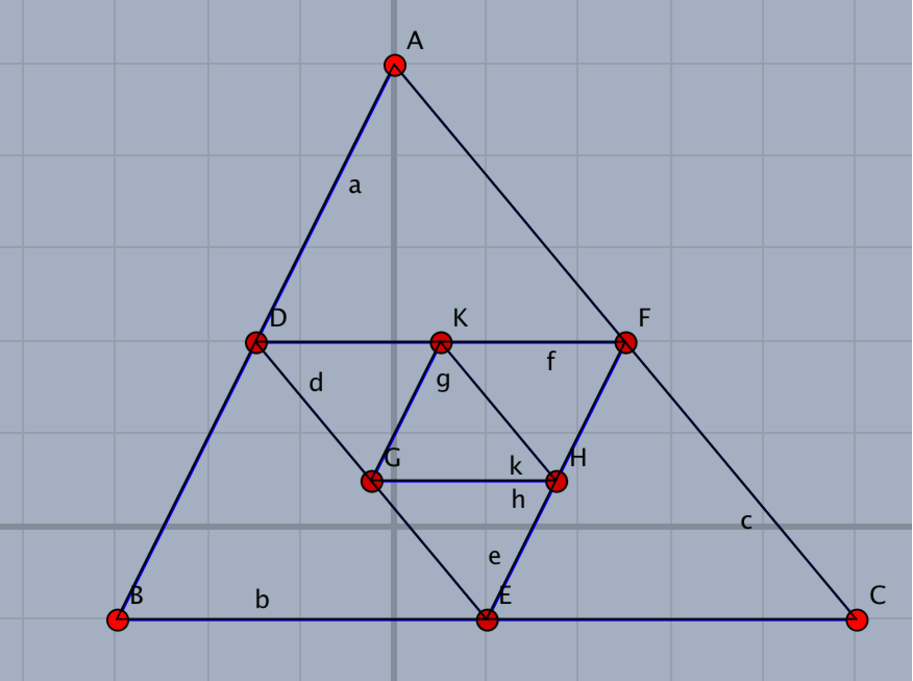
\includegraphics[bb=0.00 0.00 438.02 327.02,width=5cm]{Fig/gpro01.pdf}     %%% /Users/Hannya/Desktop/KeTCindy/fig/test.tex 
%%% Generator=template1basic.cdy 
{\unitlength=5mm%
\begin{picture}%
(11,9)(-5,-3)%
\special{pn 8}%
%
\special{pa     0  -984}\special{pa  -591   197}%
\special{fp}%
\special{pa  -591   197}\special{pa   984   197}%
\special{fp}%
\special{pa   984   197}\special{pa     0  -984}%
\special{fp}%
\special{pa  -295  -394}\special{pa   197   197}%
\special{fp}%
\special{pa   197   197}\special{pa   492  -394}%
\special{fp}%
\special{pa   492  -394}\special{pa  -295  -394}%
\special{fp}%
\special{pa    98  -394}\special{pa   -49   -98}%
\special{fp}%
\special{pa   -49   -98}\special{pa   344   -98}%
\special{fp}%
\special{pa   344   -98}\special{pa    98  -394}%
\special{fp}%
\end{picture}}%

\vspace{\baselineskip}
\hypertarget{framedata}{}
\item[関数]  Framedata(name , リスト,options)
\item[機能]  矩形を描く
\item[説明]  リストの形は2通り。

その1:[中心 ,横 , 縦] で,矩形を描く。横,縦は中心からの距離。

その2:2点のリスト。点が座標でなく名称のときはnameは省略できる。

点の座標は点の名前でもよい。点を座標で与える場合はnameは省略できない。

リストを省略した場合は,描画範囲と同一の矩形を描く。

その2のタイプでは,option として,"center" または "corner" がある。"center" のときは,中心と対角点( 初期設定),"corner" のときは2点を対角点として解釈する。 

以下にいくつか例を示す
\begin{tabbing}
1234567890123456789012345678901234\=\kill
  \verb|Framedata("1");|  \> 描画範囲(SW,NE)と同一の矩形を描く\\
  \verb|Framedata("2",[[0,0],2,2]);|   \> 原点を中心とする縦横幅4の正方形を描く\\
  \verb|Framedata("3",[A,1.5,1.2]);|  \> 点Aを中心とする横3,縦2.4の矩形を描く。(図左)\\
  \verb|Framedata([B,C]);|                  \> 点Bを中心,点Cを頂点とする矩形を描く。(図中央)\\
  \verb|Framedata([D,E],["corner"]); |        \>  点D,Eを対角点とする矩形を描く。(図右)
 \end{tabbing}
\begin{center}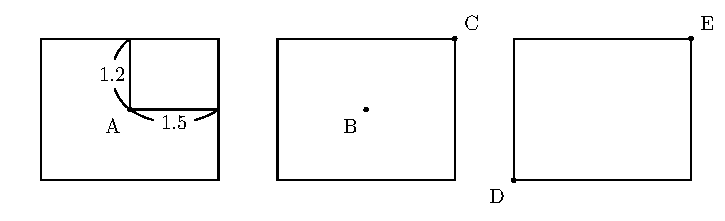
\includegraphics[bb=0.00 0.00 348.15 106.16,width=12cm]{Fig/Framedata.pdf}\end{center}

矩形の角を丸めたい場合は,Framedata()ではなく,\hyperlink{ovaldata}{Ovaldata()}を使うとよい。
 
\vspace{\baselineskip}
\hypertarget{polygonplot}{}
\item[関数]  Polygonplot(name , 点リスト , 整数,options)
\item[機能]  2点を半径とする円に内接する正多角形を描く。
\item[説明]  点リストを[A,B] とすると,Aを中心とする半径ABの円周上に点をとって正多角形を描く。ただし円は描かない。A,B は座標でもよい。

点リストが座標ではなく作図してある点の名称のとき,オプションに  "Geo=y" をつけると,頂点の幾何点を作る。幾何点の名称はBに番号を付けたものとなる。整数でない数を指定した場合は,きちんと閉じない折れ線が描かれる。

\vspace{\baselineskip}
【例】点リストとoptionの違いによる作図と,TeXの図を示す。

\begin{verbatim}
    Addax(0);
    Polygonplot("1",[[-4,1],[-4,3]],7);
    Polygonplot("2",[A,B],7);
    Polygonplot("3",[C,D],7,["Geo=y"]);
\end{verbatim}

\hspace{10mm}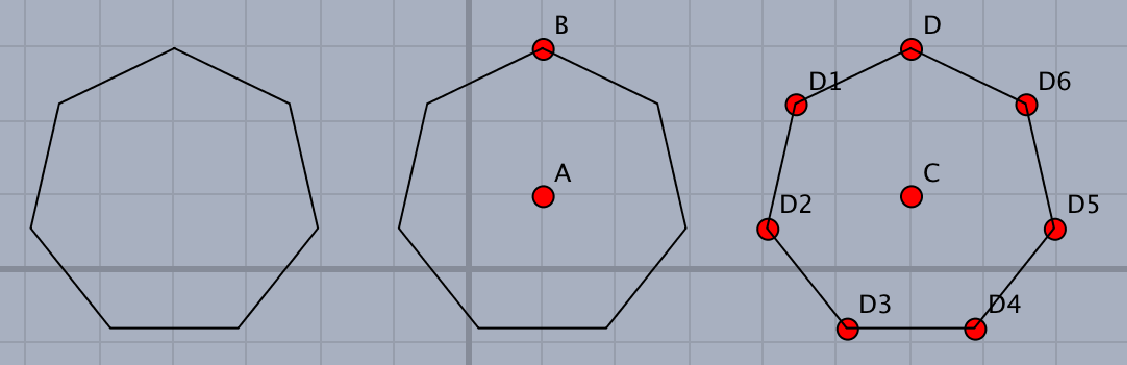
\includegraphics[bb=0.00 0.00 541.03 175.01,width=10cm]{Fig/polygonplot2.pdf}

\hspace{10mm}%%% /Users/Hannya/Desktop/KeTCindy/fig/polygonplot1.tex 
%%% Generator=template1basic.cdy 
{\unitlength=6mm%
\begin{picture}%
(16.33,5.71)(-6.82,-1.78)%
\special{pn 8}%
%
{%
\color[rgb]{0,0,0}%
\special{pa  -945  -709}\special{pa -1314  -531}\special{pa -1405  -131}\special{pa -1150   189}%
\special{pa  -740   189}\special{pa  -484  -131}\special{pa  -576  -531}\special{pa  -945  -709}%
\special{fp}%
}%
{%
\color[rgb]{0,0,0}%
\special{pa   236  -709}\special{pa  -133  -531}\special{pa  -224  -131}\special{pa    31   189}%
\special{pa   441   189}\special{pa   697  -131}\special{pa   606  -531}\special{pa   236  -709}%
\special{fp}%
}%
{%
\color[rgb]{0,0,0}%
\special{pa  1417  -709}\special{pa  1048  -531}\special{pa   957  -131}\special{pa  1212   189}%
\special{pa  1622   189}\special{pa  1878  -131}\special{pa  1787  -531}\special{pa  1417  -709}%
\special{fp}%
}%
\end{picture}}%


円に内接する形でなく,与えられた線分ABを1辺とする正多角形を描くには次のようにする。

線分ABは,Cinderellaの作図ツールなどで描かれているものとする。ただし,線分でなく,両端の点が与えられているだけでもよい。Cindyscriptで点A,Bが複素平面上にあるものとして,多角形の頂点の位置を計算する。

\vspace{\baselineskip}
【例】ABを1辺とする正五角形を描く。

\begin{verbatim}
  n=5;
  pti=[complex(A),complex(B)];
  th=2*pi/n;
  repeat(n-2,s,
    z1=pti_s;
    z2=pti_(s+1);
    z=z2+(z2-z1)*(cos(th)+i*sin(th));
    pti=append(pti,z);
  );
  pt=apply(pti,gauss(#));
  pt=append(pt,A.xy);
  Listplot("1",pt);
\end{verbatim}
ptiは,各頂点に対応する複素数のリスト,ptが各頂点の座標のリストである。 

\begin{flushright}  \hyperlink{functionlist}{$\Rightarrow$関数一覧}\end{flushright}

\end{description}
\newpage
% ====== 曲線 ==============
\subsubsection{曲線}
\begin{description}

\hypertarget{bezier}{}
\item[関数]  Bezier(名前,節点リスト,制御点リスト,[オプション] )
\item[機能]  ベジェ曲線を描く
\item[説明]  制御点は,各区間に対して,3次の場合2個,2次の場合1個のリストで与える。

オプションは

"Num=n"  : 節点間の分割数(分点数 $-1$)を指定できる。 ベジェ曲線とスプライト曲線の関数は節点間が短い場合が多いので初期設定は10になっている。Plotdata()などと違い,大きい数(200など)を指定すると,全体の分割数が増大して描画時間がかかるようになってしまうので注意。

\vspace{\baselineskip}
【例】

\begin{layer}{150}{0}
\putnotese{60}{-10}{\scalebox{0.9}{ %%% checkb.tex 2015-1-6 7:22
%%% checkb.sce 2015-1-6 6:35
{\unitlength=1cm%
\begin{picture}%
(   5.95000,   4.06000)(  -3.00000,  -2.00000)%
\special{pn 8}%
%
\special{pa -738 419}\special{pa -746 414}\special{pa -756 414}\special{pa -764 418}%
\special{pa -770 425}\special{pa -772 434}\special{pa -769 443}\special{pa -762 450}%
\special{pa -753 453}\special{pa -744 451}\special{pa -736 445}\special{pa -733 437}%
\special{pa -733 427}\special{pa -738 419}\special{sh 1}\special{fp}%
\special{pa 888 470}\special{pa 880 465}\special{pa 870 465}\special{pa 862 469}\special{pa 856 476}%
\special{pa 854 485}\special{pa 857 494}\special{pa 864 501}\special{pa 873 504}\special{pa 882 502}%
\special{pa 890 496}\special{pa 893 488}\special{pa 893 478}\special{pa 888 470}\special{sh 1}\special{fp}%
\special{pa -439 -238}\special{pa -447 -243}\special{pa -456 -244}\special{pa -465 -240}%
\special{pa -471 -232}\special{pa -472 -223}\special{pa -470 -214}\special{pa -463 -208}%
\special{pa -454 -205}\special{pa -445 -206}\special{pa -437 -212}\special{pa -433 -221}%
\special{pa -434 -230}\special{pa -439 -238}\special{sh 1}\special{fp}%
\settowidth{\Width}{A}\setlength{\Width}{-1\Width}%
\settoheight{\Height}{A}\settodepth{\Depth}{A}\setlength{\Height}{-\Height}%
\put(-2.0600,-1.2500){\hspace*{\Width}\raisebox{\Height}{A}}%
%
%
\settowidth{\Width}{B}\setlength{\Width}{0\Width}%
\settoheight{\Height}{B}\settodepth{\Depth}{B}\setlength{\Height}{-\Height}%
\put(2.3700,-1.3800){\hspace*{\Width}\raisebox{\Height}{B}}%
%
%
\settowidth{\Width}{C}\setlength{\Width}{-1\Width}%
\settoheight{\Height}{C}\settodepth{\Depth}{C}\setlength{\Height}{\Depth}%
\put(-1.3000,0.7200){\hspace*{\Width}\raisebox{\Height}{C}}%
%
%
\special{pa -752 433}\special{pa -682 315}\special{pa -591 225}\special{pa -480 162}%
\special{pa -348 126}\special{pa -196 117}\special{pa -23 136}\special{pa 170 182}%
\special{pa 384 255}\special{pa 619 356}\special{pa 874 484}%
\special{fp}%
\end{picture}}%}}
\end{layer}

2次ベジェ曲線

Bezier("1",[A,B],[C]);

\vspace{20mm}

\begin{layer}{150}{0}
\putnotese{60}{-10}{\scalebox{0.9}{%%% checkb.tex 2015-1-6 7:20
%%% checkb.sce 2015-1-6 6:35
{\unitlength=1cm%
\begin{picture}%
(   5.95000,   4.06000)(  -3.00000,  -2.00000)%
\special{pn 8}%
%
\special{pa -738 419}\special{pa -746 414}\special{pa -756 414}\special{pa -764 418}%
\special{pa -770 425}\special{pa -772 434}\special{pa -769 443}\special{pa -762 450}%
\special{pa -753 453}\special{pa -744 451}\special{pa -736 445}\special{pa -733 437}%
\special{pa -733 427}\special{pa -738 419}\special{sh 1}\special{fp}%
\special{pa 888 470}\special{pa 880 465}\special{pa 870 465}\special{pa 862 469}\special{pa 856 476}%
\special{pa 854 485}\special{pa 857 494}\special{pa 864 501}\special{pa 873 504}\special{pa 882 502}%
\special{pa 890 496}\special{pa 893 488}\special{pa 893 478}\special{pa 888 470}\special{sh 1}\special{fp}%
\special{pa -439 -238}\special{pa -447 -243}\special{pa -456 -244}\special{pa -465 -240}%
\special{pa -471 -232}\special{pa -472 -223}\special{pa -470 -214}\special{pa -463 -208}%
\special{pa -454 -205}\special{pa -445 -206}\special{pa -437 -212}\special{pa -433 -221}%
\special{pa -434 -230}\special{pa -439 -238}\special{sh 1}\special{fp}%
\special{pa 427 -282}\special{pa 419 -287}\special{pa 410 -287}\special{pa 401 -283}%
\special{pa 395 -276}\special{pa 394 -267}\special{pa 397 -258}\special{pa 403 -251}%
\special{pa 412 -248}\special{pa 421 -250}\special{pa 429 -256}\special{pa 433 -264}%
\special{pa 432 -274}\special{pa 427 -282}\special{sh 1}\special{fp}%
\settowidth{\Width}{A}\setlength{\Width}{-1\Width}%
\settoheight{\Height}{A}\settodepth{\Depth}{A}\setlength{\Height}{-\Height}%
\put(-2.0600,-1.2500){\hspace*{\Width}\raisebox{\Height}{A}}%
%
%
\settowidth{\Width}{B}\setlength{\Width}{0\Width}%
\settoheight{\Height}{B}\settodepth{\Depth}{B}\setlength{\Height}{-\Height}%
\put(2.3700,-1.3800){\hspace*{\Width}\raisebox{\Height}{B}}%
%
%
\settowidth{\Width}{C}\setlength{\Width}{-1\Width}%
\settoheight{\Height}{C}\settodepth{\Depth}{C}\setlength{\Height}{\Depth}%
\put(-1.3000,0.7200){\hspace*{\Width}\raisebox{\Height}{C}}%
%
%
\settowidth{\Width}{D}\setlength{\Width}{-1\Width}%
\settoheight{\Height}{D}\settodepth{\Depth}{D}\setlength{\Height}{\Depth}%
\put(0.9000,0.8300){\hspace*{\Width}\raisebox{\Height}{D}}%
%
%
\special{pa -752 433}\special{pa -646 254}\special{pa -512 114}\special{pa -356 12}%
\special{pa -183 -50}\special{pa 0 -70}\special{pa 189 -48}\special{pa 376 17}\special{pa 557 127}%
\special{pa 725 282}\special{pa 874 484}%
\special{fp}%
\end{picture}}%}}
\end{layer}

3次ベジェ曲線

Bezier("2",[A,B],[C,D]);

\vspace{20mm}

\begin{layer}{150}{0}
\putnotese{60}{-10}{\scalebox{0.9}{ %%% checkb.tex 2015-1-6 7:31
%%% checkb.sce 2015-1-6 6:35
{\unitlength=1cm%
\begin{picture}%
(   5.95000,   4.06000)(  -3.00000,  -2.00000)%
\special{pn 8}%
%
\special{pa -911 368}\special{pa -919 363}\special{pa -929 363}\special{pa -937 366}%
\special{pa -943 374}\special{pa -945 383}\special{pa -942 392}\special{pa -935 399}%
\special{pa -926 402}\special{pa -917 400}\special{pa -910 394}\special{pa -906 385}%
\special{pa -906 376}\special{pa -911 368}\special{sh 1}\special{fp}%
\special{pa -254 356}\special{pa -262 351}\special{pa -271 351}\special{pa -280 355}%
\special{pa -286 362}\special{pa -287 371}\special{pa -285 380}\special{pa -278 387}%
\special{pa -269 390}\special{pa -260 388}\special{pa -252 382}\special{pa -248 374}%
\special{pa -249 364}\special{pa -254 356}\special{sh 1}\special{fp}%
\special{pa 888 478}\special{pa 880 473}\special{pa 870 473}\special{pa 862 477}\special{pa 856 484}%
\special{pa 854 493}\special{pa 857 502}\special{pa 864 509}\special{pa 873 512}\special{pa 882 510}%
\special{pa 890 504}\special{pa 893 496}\special{pa 893 486}\special{pa 888 478}\special{sh 1}\special{fp}%
\special{pa -655 -45}\special{pa -663 -50}\special{pa -673 -51}\special{pa -681 -47}%
\special{pa -687 -40}\special{pa -689 -30}\special{pa -686 -21}\special{pa -679 -15}%
\special{pa -670 -12}\special{pa -661 -14}\special{pa -654 -19}\special{pa -650 -28}%
\special{pa -650 -37}\special{pa -655 -45}\special{sh 1}\special{fp}%
\special{pa 116 -53}\special{pa 108 -58}\special{pa 99 -59}\special{pa 90 -55}\special{pa 84 -47}%
\special{pa 83 -38}\special{pa 86 -29}\special{pa 92 -23}\special{pa 101 -20}\special{pa 110 -21}%
\special{pa 118 -27}\special{pa 122 -36}\special{pa 121 -45}\special{pa 116 -53}\special{sh 1}\special{fp}%
\special{pa 518 -77}\special{pa 510 -82}\special{pa 500 -82}\special{pa 492 -78}\special{pa 486 -71}%
\special{pa 484 -62}\special{pa 487 -53}\special{pa 494 -46}\special{pa 503 -43}\special{pa 512 -45}%
\special{pa 519 -51}\special{pa 523 -59}\special{pa 523 -69}\special{pa 518 -77}\special{sh 1}\special{fp}%
\settowidth{\Width}{A}\setlength{\Width}{-1\Width}%
\settoheight{\Height}{A}\settodepth{\Depth}{A}\setlength{\Height}{-\Height}%
\put(-2.5000,-1.1200){\hspace*{\Width}\raisebox{\Height}{A}}%
%
%
\settowidth{\Width}{B}\setlength{\Width}{-0.5\Width}%
\settoheight{\Height}{B}\settodepth{\Depth}{B}\setlength{\Height}{-\Height}%
\put(-0.6800,-1.0900){\hspace*{\Width}\raisebox{\Height}{B}}%
%
%
\settowidth{\Width}{C}\setlength{\Width}{0\Width}%
\settoheight{\Height}{C}\settodepth{\Depth}{C}\setlength{\Height}{-\Height}%
\put(2.3700,-1.4000){\hspace*{\Width}\raisebox{\Height}{C}}%
%
%
\settowidth{\Width}{D}\setlength{\Width}{-0.5\Width}%
\settoheight{\Height}{D}\settodepth{\Depth}{D}\setlength{\Height}{\Depth}%
\put(-1.7000,0.2300){\hspace*{\Width}\raisebox{\Height}{D}}%
%
%
\settowidth{\Width}{E}\setlength{\Width}{-1\Width}%
\settoheight{\Height}{E}\settodepth{\Depth}{E}\setlength{\Height}{\Depth}%
\put(0.1100,0.2500){\hspace*{\Width}\raisebox{\Height}{E}}%
%
%
\settowidth{\Width}{F}\setlength{\Width}{0\Width}%
\settoheight{\Height}{F}\settodepth{\Depth}{F}\setlength{\Height}{\Depth}%
\put(1.4300,0.3100){\hspace*{\Width}\raisebox{\Height}{F}}%
%
%
\special{pa -925 382}\special{pa -873 307}\special{pa -817 249}\special{pa -759 207}%
\special{pa -697 182}\special{pa -633 172}\special{pa -566 179}\special{pa -496 202}%
\special{pa -423 242}\special{pa -347 298}\special{pa -268 370}\special{pa -156 259}%
\special{pa -42 172}\special{pa 72 111}\special{pa 187 76}\special{pa 303 69}\special{pa 419 91}%
\special{pa 534 144}\special{pa 649 227}\special{pa 762 343}\special{pa 874 492}%
\special{fp}%
\end{picture}}%}}
\end{layer}

%ベジェ曲線をつなげる

%Bezier("3",[A,B,C],[[D],[E,F]]);

%\vspace{20mm}

%\begin{layer}{150}{0}
%\putnotese{60}{5}{ %%% checkb.tex 2015-1-6 8:23
%%% checkb.sce 2015-1-6 6:35
{\unitlength=1cm%
\begin{picture}%
(  14.00000,   3.95000)(  -3.03000,  -1.91000)%
\special{pn 8}%
%
\special{pa -974 -167}\special{pa -982 -172}\special{pa -992 -173}\special{pa -1000 -169}%
\special{pa -1006 -162}\special{pa -1008 -152}\special{pa -1005 -143}\special{pa -998 -137}%
\special{pa -989 -134}\special{pa -980 -136}\special{pa -973 -141}\special{pa -969 -150}%
\special{pa -969 -159}\special{pa -974 -167}\special{sh 1}\special{fp}%
\special{pa -273 -128}\special{pa -282 -133}\special{pa -291 -134}\special{pa -300 -130}%
\special{pa -305 -122}\special{pa -307 -113}\special{pa -304 -104}\special{pa -298 -97}%
\special{pa -289 -95}\special{pa -279 -96}\special{pa -272 -102}\special{pa -268 -111}%
\special{pa -269 -120}\special{pa -273 -128}\special{sh 1}\special{fp}%
\special{pa 919 -167}\special{pa 911 -172}\special{pa 902 -173}\special{pa 893 -169}%
\special{pa 888 -162}\special{pa 886 -152}\special{pa 889 -143}\special{pa 895 -137}%
\special{pa 904 -134}\special{pa 914 -136}\special{pa 921 -141}\special{pa 925 -150}%
\special{pa 924 -159}\special{pa 919 -167}\special{sh 1}\special{fp}%
\special{pa -644 -538}\special{pa -652 -542}\special{pa -661 -543}\special{pa -670 -539}%
\special{pa -675 -532}\special{pa -677 -522}\special{pa -674 -513}\special{pa -668 -507}%
\special{pa -659 -504}\special{pa -649 -506}\special{pa -642 -511}\special{pa -638 -520}%
\special{pa -639 -529}\special{pa -644 -538}\special{sh 1}\special{fp}%
\special{pa 128 305}\special{pa 120 300}\special{pa 111 300}\special{pa 102 303}\special{pa 96 311}%
\special{pa 95 320}\special{pa 97 329}\special{pa 104 336}\special{pa 113 339}\special{pa 122 337}%
\special{pa 130 331}\special{pa 134 322}\special{pa 133 313}\special{pa 128 305}\special{sh 1}\special{fp}%
\special{pa 734 325}\special{pa 726 320}\special{pa 717 319}\special{pa 708 323}\special{pa 703 331}%
\special{pa 701 340}\special{pa 704 349}\special{pa 710 355}\special{pa 719 358}\special{pa 729 357}%
\special{pa 736 351}\special{pa 740 342}\special{pa 739 333}\special{pa 734 325}\special{sh 1}\special{fp}%
\settowidth{\Width}{A}\setlength{\Width}{-1\Width}%
\settoheight{\Height}{A}\settodepth{\Depth}{A}\setlength{\Height}{-\Height}%
\put(-2.6600,0.2400){\hspace*{\Width}\raisebox{\Height}{A}}%
%
%
\settowidth{\Width}{B}\setlength{\Width}{-0.5\Width}%
\settoheight{\Height}{B}\settodepth{\Depth}{B}\setlength{\Height}{-\Height}%
\put(-0.7300,0.1400){\hspace*{\Width}\raisebox{\Height}{B}}%
%
%
\settowidth{\Width}{C}\setlength{\Width}{0\Width}%
\settoheight{\Height}{C}\settodepth{\Depth}{C}\setlength{\Height}{\Depth}%
\put(2.4500,0.5400){\hspace*{\Width}\raisebox{\Height}{C}}%
%
%
\settowidth{\Width}{D}\setlength{\Width}{-0.5\Width}%
\settoheight{\Height}{D}\settodepth{\Depth}{D}\setlength{\Height}{\Depth}%
\put(-1.6700,1.4800){\hspace*{\Width}\raisebox{\Height}{D}}%
%
%
\settowidth{\Width}{E}\setlength{\Width}{-1\Width}%
\settoheight{\Height}{E}\settodepth{\Depth}{E}\setlength{\Height}{-\Height}%
\put(0.1400,-0.9600){\hspace*{\Width}\raisebox{\Height}{E}}%
%
%
\settowidth{\Width}{F}\setlength{\Width}{0\Width}%
\settoheight{\Height}{F}\settodepth{\Depth}{F}\setlength{\Height}{-\Height}%
\put(1.9800,-1.0100){\hspace*{\Width}\raisebox{\Height}{F}}%
%
%
\special{pa -988 -154}\special{pa -922 -220}\special{pa -854 -270}\special{pa -786 -305}%
\special{pa -717 -325}\special{pa -648 -329}\special{pa -577 -317}\special{pa -506 -290}%
\special{pa -434 -247}\special{pa -361 -188}\special{pa -287 -114}\special{pa -161 3}%
\special{pa -27 95}\special{pa 112 161}\special{pa 253 201}\special{pa 390 213}\special{pa 521 198}%
\special{pa 642 154}\special{pa 749 81}\special{pa 838 -21}\special{pa 906 -154}%
\special{fp}%
\end{picture}}%}
%\end{layer}

%D,B,E を1直線上にとると,滑らかにつながる
節点を増やす。2次と3次。

Bezier("3",[A,B,C],[[D],[E,F]]);

\vspace{20mm}

全て同じ次数の場合,次のようにしてもよい.

Bezier("4", [A,B,C,D], [E,F,G,H,K,L] );   

\begin{layer}{150}{0}
\putnotese{20}{2}{%%% checkb.tex 2015-1-13 20:23
%%% checkb.sce 2015-1-13 13:55
{\unitlength=1cm%
\begin{picture}%
(  11.00000,   2.95000)(  -4.99000,  -0.99000)%
\special{pn 8}%
%
\special{pa -1472 173}\special{pa -1407 65}\special{pa -1323 -21}\special{pa -1224 -85}%
\special{pa -1114 -128}\special{pa -997 -149}\special{pa -876 -150}\special{pa -754 -130}%
\special{pa -635 -89}\special{pa -523 -29}\special{pa -421 51}\special{pa -312 -68}%
\special{pa -182 -172}\special{pa -38 -255}\special{pa 114 -314}\special{pa 271 -344}%
\special{pa 426 -343}\special{pa 575 -306}\special{pa 711 -228}\special{pa 829 -107}%
\special{pa 925 63}\special{pa 1009 -73}\special{pa 1105 -167}\special{pa 1208 -223}%
\special{pa 1315 -246}\special{pa 1423 -240}\special{pa 1526 -209}\special{pa 1622 -157}%
\special{pa 1706 -88}\special{pa 1774 -7}\special{pa 1823 83}%
\special{fp}%
\special{pa -1459 159}\special{pa -1467 154}\special{pa -1476 154}\special{pa -1485 158}%
\special{pa -1490 165}\special{pa -1492 174}\special{pa -1489 183}\special{pa -1483 190}%
\special{pa -1474 193}\special{pa -1464 191}\special{pa -1457 185}\special{pa -1453 177}%
\special{pa -1454 167}\special{pa -1459 159}\special{sh 1}\special{fp}%
\special{pa -407 37}\special{pa -415 32}\special{pa -425 32}\special{pa -433 36}\special{pa -439 43}%
\special{pa -441 52}\special{pa -438 61}\special{pa -431 68}\special{pa -422 71}\special{pa -413 69}%
\special{pa -406 63}\special{pa -402 55}\special{pa -402 45}\special{pa -407 37}\special{sh 1}\special{fp}%
\special{pa 939 49}\special{pa 931 44}\special{pa 922 44}\special{pa 913 47}\special{pa 907 55}%
\special{pa 906 64}\special{pa 908 73}\special{pa 915 80}\special{pa 924 83}\special{pa 933 81}%
\special{pa 941 75}\special{pa 945 67}\special{pa 944 57}\special{pa 939 49}\special{sh 1}\special{fp}%
\special{pa 1837 69}\special{pa 1829 64}\special{pa 1819 63}\special{pa 1811 67}\special{pa 1805 75}%
\special{pa 1803 84}\special{pa 1806 93}\special{pa 1813 100}\special{pa 1822 102}%
\special{pa 1831 101}\special{pa 1838 95}\special{pa 1842 86}\special{pa 1842 77}%
\special{pa 1837 69}\special{sh 1}\special{fp}%
\special{pa -1273 -238}\special{pa -1282 -243}\special{pa -1291 -244}\special{pa -1300 -240}%
\special{pa -1305 -232}\special{pa -1307 -223}\special{pa -1304 -214}\special{pa -1298 -208}%
\special{pa -1289 -205}\special{pa -1279 -206}\special{pa -1272 -212}\special{pa -1268 -221}%
\special{pa -1269 -230}\special{pa -1273 -238}\special{sh 1}\special{fp}%
\special{pa -726 -262}\special{pa -734 -267}\special{pa -744 -267}\special{pa -752 -264}%
\special{pa -758 -256}\special{pa -760 -247}\special{pa -757 -238}\special{pa -750 -231}%
\special{pa -741 -228}\special{pa -732 -230}\special{pa -725 -236}\special{pa -721 -244}%
\special{pa -721 -254}\special{pa -726 -262}\special{sh 1}\special{fp}%
\special{pa -81 -384}\special{pa -89 -389}\special{pa -98 -389}\special{pa -107 -386}%
\special{pa -112 -378}\special{pa -114 -369}\special{pa -111 -360}\special{pa -105 -353}%
\special{pa -96 -350}\special{pa -86 -352}\special{pa -79 -358}\special{pa -75 -367}%
\special{pa -76 -376}\special{pa -81 -384}\special{sh 1}\special{fp}%
\special{pa 664 -601}\special{pa 655 -605}\special{pa 646 -606}\special{pa 637 -602}%
\special{pa 632 -595}\special{pa 630 -585}\special{pa 633 -576}\special{pa 639 -570}%
\special{pa 648 -567}\special{pa 658 -569}\special{pa 665 -574}\special{pa 669 -583}%
\special{pa 668 -592}\special{pa 664 -601}\special{sh 1}\special{fp}%
\special{pa 1195 -478}\special{pa 1187 -483}\special{pa 1178 -484}\special{pa 1169 -480}%
\special{pa 1163 -473}\special{pa 1161 -463}\special{pa 1164 -454}\special{pa 1171 -448}%
\special{pa 1180 -445}\special{pa 1189 -447}\special{pa 1197 -452}\special{pa 1200 -461}%
\special{pa 1200 -470}\special{pa 1195 -478}\special{sh 1}\special{fp}%
\special{pa 1711 -238}\special{pa 1703 -243}\special{pa 1693 -244}\special{pa 1685 -240}%
\special{pa 1679 -232}\special{pa 1677 -223}\special{pa 1680 -214}\special{pa 1687 -208}%
\special{pa 1696 -205}\special{pa 1705 -206}\special{pa 1712 -212}\special{pa 1716 -221}%
\special{pa 1716 -230}\special{pa 1711 -238}\special{sh 1}\special{fp}%
\settowidth{\Width}{A}\setlength{\Width}{-0.5\Width}%
\settoheight{\Height}{A}\settodepth{\Depth}{A}\setlength{\Height}{-\Height}%
\put(-3.7400,-0.5900){\hspace*{\Width}\raisebox{\Height}{A}}%
%
%
\settowidth{\Width}{B}\setlength{\Width}{-0.5\Width}%
\settoheight{\Height}{B}\settodepth{\Depth}{B}\setlength{\Height}{-\Height}%
\put(-1.0700,-0.2800){\hspace*{\Width}\raisebox{\Height}{B}}%
%
%
\settowidth{\Width}{C}\setlength{\Width}{-0.5\Width}%
\settoheight{\Height}{C}\settodepth{\Depth}{C}\setlength{\Height}{-\Height}%
\put(2.3500,-0.3100){\hspace*{\Width}\raisebox{\Height}{C}}%
%
%
\settowidth{\Width}{D}\setlength{\Width}{-0.5\Width}%
\settoheight{\Height}{D}\settodepth{\Depth}{D}\setlength{\Height}{-\Height}%
\put(4.6300,-0.3600){\hspace*{\Width}\raisebox{\Height}{D}}%
%
%
\settowidth{\Width}{E}\setlength{\Width}{-0.5\Width}%
\settoheight{\Height}{E}\settodepth{\Depth}{E}\setlength{\Height}{\Depth}%
\put(-3.2700,0.7200){\hspace*{\Width}\raisebox{\Height}{E}}%
%
%
\settowidth{\Width}{F}\setlength{\Width}{-0.5\Width}%
\settoheight{\Height}{F}\settodepth{\Depth}{F}\setlength{\Height}{\Depth}%
\put(-1.8800,0.7800){\hspace*{\Width}\raisebox{\Height}{F}}%
%
%
\settowidth{\Width}{G}\setlength{\Width}{-0.5\Width}%
\settoheight{\Height}{G}\settodepth{\Depth}{G}\setlength{\Height}{\Depth}%
\put(-0.2400,1.0900){\hspace*{\Width}\raisebox{\Height}{G}}%
%
%
\settowidth{\Width}{H}\setlength{\Width}{-0.5\Width}%
\settoheight{\Height}{H}\settodepth{\Depth}{H}\setlength{\Height}{\Depth}%
\put(1.6500,1.6400){\hspace*{\Width}\raisebox{\Height}{H}}%
%
%
\settowidth{\Width}{K}\setlength{\Width}{-0.5\Width}%
\settoheight{\Height}{K}\settodepth{\Depth}{K}\setlength{\Height}{\Depth}%
\put(3.0000,1.3300){\hspace*{\Width}\raisebox{\Height}{K}}%
%
%
\settowidth{\Width}{L}\setlength{\Width}{-0.5\Width}%
\settoheight{\Height}{L}\settodepth{\Depth}{L}\setlength{\Height}{\Depth}%
\put(4.3100,0.7200){\hspace*{\Width}\raisebox{\Height}{L}}%
%
%
\end{picture}}%}
\end{layer}

\vspace{35mm}

オプションの例

Bezier("5",[A,B,C],[[D],[E,F]],["Num=3"]);

\hspace{20mm}%%% checkb.tex 2015-1-6 8:30
%%% checkb.sce 2015-1-6 6:35
{\unitlength=1cm%
\begin{picture}%
(  14.00000,   3.95000)(  -3.03000,  -1.91000)%
\special{pn 8}%
%
\special{pa -974 -167}\special{pa -982 -172}\special{pa -992 -173}\special{pa -1000 -169}%
\special{pa -1006 -162}\special{pa -1008 -152}\special{pa -1005 -143}\special{pa -998 -137}%
\special{pa -989 -134}\special{pa -980 -136}\special{pa -973 -141}\special{pa -969 -150}%
\special{pa -969 -159}\special{pa -974 -167}\special{sh 1}\special{fp}%
\special{pa -273 -128}\special{pa -282 -133}\special{pa -291 -134}\special{pa -300 -130}%
\special{pa -305 -122}\special{pa -307 -113}\special{pa -304 -104}\special{pa -298 -97}%
\special{pa -289 -95}\special{pa -279 -96}\special{pa -272 -102}\special{pa -268 -111}%
\special{pa -269 -120}\special{pa -273 -128}\special{sh 1}\special{fp}%
\special{pa 919 -167}\special{pa 911 -172}\special{pa 902 -173}\special{pa 893 -169}%
\special{pa 888 -162}\special{pa 886 -152}\special{pa 889 -143}\special{pa 895 -137}%
\special{pa 904 -134}\special{pa 914 -136}\special{pa 921 -141}\special{pa 925 -150}%
\special{pa 924 -159}\special{pa 919 -167}\special{sh 1}\special{fp}%
\special{pa -644 -538}\special{pa -652 -542}\special{pa -661 -543}\special{pa -670 -539}%
\special{pa -675 -532}\special{pa -677 -522}\special{pa -674 -513}\special{pa -668 -507}%
\special{pa -659 -504}\special{pa -649 -506}\special{pa -642 -511}\special{pa -638 -520}%
\special{pa -639 -529}\special{pa -644 -538}\special{sh 1}\special{fp}%
\special{pa 128 305}\special{pa 120 300}\special{pa 111 300}\special{pa 102 303}\special{pa 96 311}%
\special{pa 95 320}\special{pa 97 329}\special{pa 104 336}\special{pa 113 339}\special{pa 122 337}%
\special{pa 130 331}\special{pa 134 322}\special{pa 133 313}\special{pa 128 305}\special{sh 1}\special{fp}%
\special{pa 734 325}\special{pa 726 320}\special{pa 717 319}\special{pa 708 323}\special{pa 703 331}%
\special{pa 701 340}\special{pa 704 349}\special{pa 710 355}\special{pa 719 358}\special{pa 729 357}%
\special{pa 736 351}\special{pa 740 342}\special{pa 739 333}\special{pa 734 325}\special{sh 1}\special{fp}%
\settowidth{\Width}{A}\setlength{\Width}{-1\Width}%
\settoheight{\Height}{A}\settodepth{\Depth}{A}\setlength{\Height}{-\Height}%
\put(-2.6600,0.2400){\hspace*{\Width}\raisebox{\Height}{A}}%
%
%
\settowidth{\Width}{B}\setlength{\Width}{-0.5\Width}%
\settoheight{\Height}{B}\settodepth{\Depth}{B}\setlength{\Height}{-\Height}%
\put(-0.7300,0.1400){\hspace*{\Width}\raisebox{\Height}{B}}%
%
%
\settowidth{\Width}{C}\setlength{\Width}{0\Width}%
\settoheight{\Height}{C}\settodepth{\Depth}{C}\setlength{\Height}{\Depth}%
\put(2.4500,0.5400){\hspace*{\Width}\raisebox{\Height}{C}}%
%
%
\settowidth{\Width}{D}\setlength{\Width}{-0.5\Width}%
\settoheight{\Height}{D}\settodepth{\Depth}{D}\setlength{\Height}{\Depth}%
\put(-1.6700,1.4800){\hspace*{\Width}\raisebox{\Height}{D}}%
%
%
\settowidth{\Width}{E}\setlength{\Width}{-1\Width}%
\settoheight{\Height}{E}\settodepth{\Depth}{E}\setlength{\Height}{-\Height}%
\put(0.1400,-0.9600){\hspace*{\Width}\raisebox{\Height}{E}}%
%
%
\settowidth{\Width}{F}\setlength{\Width}{0\Width}%
\settoheight{\Height}{F}\settodepth{\Depth}{F}\setlength{\Height}{-\Height}%
\put(1.9800,-1.0100){\hspace*{\Width}\raisebox{\Height}{F}}%
%
%
\special{pa -988 -154}\special{pa -763 -314}\special{pa -530 -301}\special{pa -287 -114}%
\special{pa 159 177}\special{pa 603 172}\special{pa 906 -154}%
\special{fp}%
\end{picture}}%

Bezier("6",[A,B,C],[[D],[E,F]],["Num=40","da"]);

\hspace{20mm}%%% checkb.tex 2015-1-6 9:16
%%% checkb.sce 2015-1-6 6:35
{\unitlength=1cm%
\begin{picture}%
(  14.00000,   3.95000)(  -3.03000,  -1.91000)%
\special{pn 8}%
%
\special{pa -988 -154}\special{pa -985 -157}\special{pa -982 -161}\special{pa -978 -164}\special{pa -975 -168}\special{pa -972 -172}\special{pa -968 -175}\special{pa -965 -178}\special{pa -962 -182}\special{fp}%
\special{pa -934 -209}\special{pa -932 -211}\special{pa -928 -214}\special{pa -925 -217}\special{pa -922 -220}\special{pa -918 -223}\special{pa -915 -226}\special{pa -912 -228}\special{pa -908 -231}\special{pa -905 -234}\special{fp}%
\special{pa -874 -257}\special{pa -871 -259}\special{pa -868 -262}\special{pa -864 -264}\special{pa -861 -266}\special{pa -858 -268}\special{pa -854 -270}\special{pa -851 -273}\special{pa -848 -275}\special{pa -844 -277}\special{pa -842 -278}\special{fp}%
\special{pa -808 -296}\special{pa -807 -297}\special{pa -803 -298}\special{pa -800 -300}\special{pa -796 -301}\special{pa -793 -303}\special{pa -790 -304}\special{pa -786 -305}\special{pa -783 -307}\special{pa -779 -308}\special{pa -776 -309}\special{pa -773 -311}\special{pa -772 -311}\special{fp}%
\special{pa -735 -321}\special{pa -735 -321}\special{pa -731 -322}\special{pa -728 -323}\special{pa -724 -324}\special{pa -721 -324}\special{pa -717 -325}\special{pa -714 -325}\special{pa -710 -326}\special{pa -707 -326}\special{pa -703 -327}\special{pa -700 -327}\special{pa -697 -328}\special{fp}%
\special{pa -658 -329}\special{pa -658 -329}\special{pa -655 -329}\special{pa -651 -329}\special{pa -648 -329}\special{pa -644 -329}\special{pa -641 -328}\special{pa -637 -328}\special{pa -634 -328}\special{pa -630 -327}\special{pa -627 -327}\special{pa -623 -326}\special{pa -620 -326}\special{fp}%
\special{pa -582 -318}\special{pa -581 -318}\special{pa -577 -317}\special{pa -574 -316}\special{pa -570 -315}\special{pa -567 -314}\special{pa -563 -313}\special{pa -559 -312}\special{pa -556 -310}\special{pa -552 -309}\special{pa -549 -308}\special{pa -545 -307}\special{fp}%
\special{pa -510 -292}\special{pa -509 -291}\special{pa -506 -290}\special{pa -502 -288}\special{pa -499 -286}\special{pa -495 -284}\special{pa -492 -282}\special{pa -488 -280}\special{pa -484 -278}\special{pa -481 -276}\special{pa -477 -274}\special{pa -476 -274}\special{fp}%
\special{pa -443 -253}\special{pa -441 -252}\special{pa -437 -249}\special{pa -434 -247}\special{pa -430 -244}\special{pa -427 -242}\special{pa -423 -239}\special{pa -419 -236}\special{pa -416 -234}\special{pa -412 -231}\special{pa -412 -231}\special{fp}%
\special{pa -382 -206}\special{pa -379 -204}\special{pa -376 -201}\special{pa -372 -198}\special{pa -368 -195}\special{pa -365 -192}\special{pa -361 -188}\special{pa -357 -185}\special{pa -354 -182}\special{pa -353 -181}\special{fp}%
\special{pa -325 -154}\special{pa -324 -153}\special{pa -321 -149}\special{pa -317 -146}\special{pa -313 -142}\special{pa -310 -138}\special{pa -306 -134}\special{pa -302 -130}\special{pa -298 -126}\special{pa -298 -126}\special{fp}%
\special{pa -272 -98}\special{pa -269 -95}\special{pa -263 -89}\special{pa -257 -82}\special{pa -251 -76}\special{pa -245 -71}\special{fp}%
\special{pa -217 -44}\special{pa -213 -41}\special{pa -207 -35}\special{pa -200 -29}\special{pa -194 -24}\special{pa -188 -19}\special{fp}%
\special{pa -158 6}\special{pa -155 8}\special{pa -148 14}\special{pa -142 19}\special{pa -135 24}\special{pa -128 29}\special{pa -128 29}\special{fp}%
\special{pa -96 52}\special{pa -95 52}\special{pa -88 57}\special{pa -81 62}\special{pa -75 66}\special{pa -68 70}\special{pa -64 73}\special{fp}%
\special{pa -31 93}\special{pa -27 95}\special{pa -20 99}\special{pa -13 103}\special{pa -6 107}\special{pa 1 111}\special{pa 3 112}\special{fp}%
\special{pa 37 129}\special{pa 42 132}\special{pa 49 135}\special{pa 56 138}\special{pa 63 141}\special{pa 70 144}\special{pa 72 145}\special{fp}%
\special{pa 108 160}\special{pa 112 161}\special{pa 119 164}\special{pa 126 166}\special{pa 133 169}\special{pa 140 171}\special{pa 144 173}\special{fp}%
\special{pa 181 184}\special{pa 183 184}\special{pa 190 186}\special{pa 197 188}\special{pa 204 190}\special{pa 211 192}\special{pa 218 193}\special{pa 219 194}\special{fp}%
\special{pa 256 201}\special{pa 260 202}\special{pa 267 203}\special{pa 274 204}\special{pa 281 205}\special{pa 287 206}\special{pa 294 207}\special{pa 294 207}\special{fp}%
\special{pa 333 211}\special{pa 336 211}\special{pa 343 212}\special{pa 349 212}\special{pa 356 213}\special{pa 363 213}\special{pa 370 213}\special{pa 371 213}\special{fp}%
\special{pa 410 213}\special{pa 410 213}\special{pa 417 212}\special{pa 424 212}\special{pa 430 211}\special{pa 437 211}\special{pa 444 210}\special{pa 448 210}\special{fp}%
\special{pa 487 205}\special{pa 489 204}\special{pa 496 203}\special{pa 502 202}\special{pa 509 200}\special{pa 515 199}\special{pa 521 198}\special{pa 524 197}\special{fp}%
\special{pa 562 187}\special{pa 565 186}\special{pa 571 184}\special{pa 577 181}\special{pa 583 179}\special{pa 589 177}\special{pa 595 175}\special{pa 598 174}\special{fp}%
\special{pa 633 158}\special{pa 636 157}\special{pa 642 154}\special{pa 648 151}\special{pa 654 148}\special{pa 659 145}\special{pa 665 142}\special{pa 667 140}\special{fp}%
\special{pa 700 119}\special{pa 703 117}\special{pa 708 114}\special{pa 713 110}\special{pa 719 106}\special{pa 724 102}\special{pa 729 98}\special{pa 731 96}\special{fp}%
\special{pa 760 71}\special{pa 764 68}\special{pa 768 63}\special{pa 773 58}\special{pa 778 54}\special{pa 782 49}\special{pa 787 44}\special{pa 787 44}\special{fp}%
\special{pa 812 14}\special{pa 813 13}\special{pa 818 7}\special{pa 822 2}\special{pa 826 -4}\special{pa 830 -10}\special{pa 834 -15}\special{pa 835 -17}\special{fp}%
\special{pa 856 -49}\special{pa 857 -51}\special{pa 861 -58}\special{pa 864 -64}\special{pa 868 -70}\special{pa 871 -77}\special{pa 874 -83}\special{fp}%
\special{pa 891 -118}\special{pa 894 -125}\special{pa 897 -132}\special{pa 900 -139}\special{pa 903 -146}\special{pa 906 -154}\special{fp}%
%
%
\special{pa -974 -167}\special{pa -982 -172}\special{pa -992 -173}\special{pa -1000 -169}%
\special{pa -1006 -162}\special{pa -1008 -152}\special{pa -1005 -143}\special{pa -998 -137}%
\special{pa -989 -134}\special{pa -980 -136}\special{pa -973 -141}\special{pa -969 -150}%
\special{pa -969 -159}\special{pa -974 -167}\special{sh 1}\special{fp}%
\special{pa -273 -128}\special{pa -282 -133}\special{pa -291 -134}\special{pa -300 -130}%
\special{pa -305 -122}\special{pa -307 -113}\special{pa -304 -104}\special{pa -298 -97}%
\special{pa -289 -95}\special{pa -279 -96}\special{pa -272 -102}\special{pa -268 -111}%
\special{pa -269 -120}\special{pa -273 -128}\special{sh 1}\special{fp}%
\special{pa 919 -167}\special{pa 911 -172}\special{pa 902 -173}\special{pa 893 -169}%
\special{pa 888 -162}\special{pa 886 -152}\special{pa 889 -143}\special{pa 895 -137}%
\special{pa 904 -134}\special{pa 914 -136}\special{pa 921 -141}\special{pa 925 -150}%
\special{pa 924 -159}\special{pa 919 -167}\special{sh 1}\special{fp}%
\special{pa -644 -538}\special{pa -652 -542}\special{pa -661 -543}\special{pa -670 -539}%
\special{pa -675 -532}\special{pa -677 -522}\special{pa -674 -513}\special{pa -668 -507}%
\special{pa -659 -504}\special{pa -649 -506}\special{pa -642 -511}\special{pa -638 -520}%
\special{pa -639 -529}\special{pa -644 -538}\special{sh 1}\special{fp}%
\special{pa 128 305}\special{pa 120 300}\special{pa 111 300}\special{pa 102 303}\special{pa 96 311}%
\special{pa 95 320}\special{pa 97 329}\special{pa 104 336}\special{pa 113 339}\special{pa 122 337}%
\special{pa 130 331}\special{pa 134 322}\special{pa 133 313}\special{pa 128 305}\special{sh 1}\special{fp}%
\special{pa 734 325}\special{pa 726 320}\special{pa 717 319}\special{pa 708 323}\special{pa 703 331}%
\special{pa 701 340}\special{pa 704 349}\special{pa 710 355}\special{pa 719 358}\special{pa 729 357}%
\special{pa 736 351}\special{pa 740 342}\special{pa 739 333}\special{pa 734 325}\special{sh 1}\special{fp}%
\settowidth{\Width}{A}\setlength{\Width}{-1\Width}%
\settoheight{\Height}{A}\settodepth{\Depth}{A}\setlength{\Height}{-\Height}%
\put(-2.6600,0.2400){\hspace*{\Width}\raisebox{\Height}{A}}%
%
%
\settowidth{\Width}{B}\setlength{\Width}{-0.5\Width}%
\settoheight{\Height}{B}\settodepth{\Depth}{B}\setlength{\Height}{-\Height}%
\put(-0.7300,0.1400){\hspace*{\Width}\raisebox{\Height}{B}}%
%
%
\settowidth{\Width}{C}\setlength{\Width}{0\Width}%
\settoheight{\Height}{C}\settodepth{\Depth}{C}\setlength{\Height}{\Depth}%
\put(2.4500,0.5400){\hspace*{\Width}\raisebox{\Height}{C}}%
%
%
\settowidth{\Width}{D}\setlength{\Width}{-0.5\Width}%
\settoheight{\Height}{D}\settodepth{\Depth}{D}\setlength{\Height}{\Depth}%
\put(-1.6700,1.4800){\hspace*{\Width}\raisebox{\Height}{D}}%
%
%
\settowidth{\Width}{E}\setlength{\Width}{-1\Width}%
\settoheight{\Height}{E}\settodepth{\Depth}{E}\setlength{\Height}{-\Height}%
\put(0.1400,-0.9600){\hspace*{\Width}\raisebox{\Height}{E}}%
%
%
\settowidth{\Width}{F}\setlength{\Width}{0\Width}%
\settoheight{\Height}{F}\settodepth{\Depth}{F}\setlength{\Height}{-\Height}%
\put(1.9800,-1.0100){\hspace*{\Width}\raisebox{\Height}{F}}%
%
%
\end{picture}}%

Numを(ベクトルとして)区間ごとに与えることもできる。

Bezier("1", [A,B,C,D], [E,F,G,H,K,L] , [ "Num=[2,3,4]"]);  

\hspace{10mm} %%% checkb.tex 2015-1-13 21:9
%%% checkb.sce 2015-1-13 13:55
{\unitlength=1cm%
\begin{picture}%
(  11.00000,   2.95000)(  -4.99000,  -0.99000)%
\special{pn 8}%
%
\special{pa -1472 173}\special{pa -997 -149}\special{pa -421 51}\special{pa 12 -277}%
\special{pa 526 -322}\special{pa 925 63}\special{pa 1156 -200}\special{pa 1423 -240}%
\special{pa 1665 -124}\special{pa 1823 83}%
\special{fp}%
\special{pa -1459 159}\special{pa -1467 154}\special{pa -1476 154}\special{pa -1485 158}%
\special{pa -1490 165}\special{pa -1492 174}\special{pa -1489 183}\special{pa -1483 190}%
\special{pa -1474 193}\special{pa -1464 191}\special{pa -1457 185}\special{pa -1453 177}%
\special{pa -1454 167}\special{pa -1459 159}\special{sh 1}\special{fp}%
\special{pa -407 37}\special{pa -415 32}\special{pa -425 32}\special{pa -433 36}\special{pa -439 43}%
\special{pa -441 52}\special{pa -438 61}\special{pa -431 68}\special{pa -422 71}\special{pa -413 69}%
\special{pa -406 63}\special{pa -402 55}\special{pa -402 45}\special{pa -407 37}\special{sh 1}\special{fp}%
\special{pa 939 49}\special{pa 931 44}\special{pa 922 44}\special{pa 913 47}\special{pa 907 55}%
\special{pa 906 64}\special{pa 908 73}\special{pa 915 80}\special{pa 924 83}\special{pa 933 81}%
\special{pa 941 75}\special{pa 945 67}\special{pa 944 57}\special{pa 939 49}\special{sh 1}\special{fp}%
\special{pa 1837 69}\special{pa 1829 64}\special{pa 1819 63}\special{pa 1811 67}\special{pa 1805 75}%
\special{pa 1803 84}\special{pa 1806 93}\special{pa 1813 100}\special{pa 1822 102}%
\special{pa 1831 101}\special{pa 1838 95}\special{pa 1842 86}\special{pa 1842 77}%
\special{pa 1837 69}\special{sh 1}\special{fp}%
\special{pa -1273 -238}\special{pa -1282 -243}\special{pa -1291 -244}\special{pa -1300 -240}%
\special{pa -1305 -232}\special{pa -1307 -223}\special{pa -1304 -214}\special{pa -1298 -208}%
\special{pa -1289 -205}\special{pa -1279 -206}\special{pa -1272 -212}\special{pa -1268 -221}%
\special{pa -1269 -230}\special{pa -1273 -238}\special{sh 1}\special{fp}%
\special{pa -726 -262}\special{pa -734 -267}\special{pa -744 -267}\special{pa -752 -264}%
\special{pa -758 -256}\special{pa -760 -247}\special{pa -757 -238}\special{pa -750 -231}%
\special{pa -741 -228}\special{pa -732 -230}\special{pa -725 -236}\special{pa -721 -244}%
\special{pa -721 -254}\special{pa -726 -262}\special{sh 1}\special{fp}%
\special{pa -81 -384}\special{pa -89 -389}\special{pa -98 -389}\special{pa -107 -386}%
\special{pa -112 -378}\special{pa -114 -369}\special{pa -111 -360}\special{pa -105 -353}%
\special{pa -96 -350}\special{pa -86 -352}\special{pa -79 -358}\special{pa -75 -367}%
\special{pa -76 -376}\special{pa -81 -384}\special{sh 1}\special{fp}%
\special{pa 664 -601}\special{pa 655 -605}\special{pa 646 -606}\special{pa 637 -602}%
\special{pa 632 -595}\special{pa 630 -585}\special{pa 633 -576}\special{pa 639 -570}%
\special{pa 648 -567}\special{pa 658 -569}\special{pa 665 -574}\special{pa 669 -583}%
\special{pa 668 -592}\special{pa 664 -601}\special{sh 1}\special{fp}%
\special{pa 1195 -478}\special{pa 1187 -483}\special{pa 1178 -484}\special{pa 1169 -480}%
\special{pa 1163 -473}\special{pa 1161 -463}\special{pa 1164 -454}\special{pa 1171 -448}%
\special{pa 1180 -445}\special{pa 1189 -447}\special{pa 1197 -452}\special{pa 1200 -461}%
\special{pa 1200 -470}\special{pa 1195 -478}\special{sh 1}\special{fp}%
\special{pa 1711 -238}\special{pa 1703 -243}\special{pa 1693 -244}\special{pa 1685 -240}%
\special{pa 1679 -232}\special{pa 1677 -223}\special{pa 1680 -214}\special{pa 1687 -208}%
\special{pa 1696 -205}\special{pa 1705 -206}\special{pa 1712 -212}\special{pa 1716 -221}%
\special{pa 1716 -230}\special{pa 1711 -238}\special{sh 1}\special{fp}%
\settowidth{\Width}{A}\setlength{\Width}{-0.5\Width}%
\settoheight{\Height}{A}\settodepth{\Depth}{A}\setlength{\Height}{-\Height}%
\put(-3.7400,-0.5900){\hspace*{\Width}\raisebox{\Height}{A}}%
%
%
\settowidth{\Width}{B}\setlength{\Width}{-0.5\Width}%
\settoheight{\Height}{B}\settodepth{\Depth}{B}\setlength{\Height}{-\Height}%
\put(-1.0700,-0.2800){\hspace*{\Width}\raisebox{\Height}{B}}%
%
%
\settowidth{\Width}{C}\setlength{\Width}{-0.5\Width}%
\settoheight{\Height}{C}\settodepth{\Depth}{C}\setlength{\Height}{-\Height}%
\put(2.3500,-0.3100){\hspace*{\Width}\raisebox{\Height}{C}}%
%
%
\settowidth{\Width}{D}\setlength{\Width}{-0.5\Width}%
\settoheight{\Height}{D}\settodepth{\Depth}{D}\setlength{\Height}{-\Height}%
\put(4.6300,-0.3600){\hspace*{\Width}\raisebox{\Height}{D}}%
%
%
\settowidth{\Width}{E}\setlength{\Width}{-0.5\Width}%
\settoheight{\Height}{E}\settodepth{\Depth}{E}\setlength{\Height}{\Depth}%
\put(-3.2700,0.7200){\hspace*{\Width}\raisebox{\Height}{E}}%
%
%
\settowidth{\Width}{F}\setlength{\Width}{-0.5\Width}%
\settoheight{\Height}{F}\settodepth{\Depth}{F}\setlength{\Height}{\Depth}%
\put(-1.8800,0.7800){\hspace*{\Width}\raisebox{\Height}{F}}%
%
%
\settowidth{\Width}{G}\setlength{\Width}{-0.5\Width}%
\settoheight{\Height}{G}\settodepth{\Depth}{G}\setlength{\Height}{\Depth}%
\put(-0.2400,1.0900){\hspace*{\Width}\raisebox{\Height}{G}}%
%
%
\settowidth{\Width}{H}\setlength{\Width}{-0.5\Width}%
\settoheight{\Height}{H}\settodepth{\Depth}{H}\setlength{\Height}{\Depth}%
\put(1.6500,1.6400){\hspace*{\Width}\raisebox{\Height}{H}}%
%
%
\settowidth{\Width}{K}\setlength{\Width}{-0.5\Width}%
\settoheight{\Height}{K}\settodepth{\Depth}{K}\setlength{\Height}{\Depth}%
\put(3.0000,1.3300){\hspace*{\Width}\raisebox{\Height}{K}}%
%
%
\settowidth{\Width}{L}\setlength{\Width}{-0.5\Width}%
\settoheight{\Height}{L}\settodepth{\Depth}{L}\setlength{\Height}{\Depth}%
\put(4.3100,0.7200){\hspace*{\Width}\raisebox{\Height}{L}}%
%
%
\end{picture}}%

%\begin{flushright}  \hyperlink{functionlist}{$\Rightarrow$関数一覧}\end{flushright}

\vspace{\baselineskip}
\hypertarget{beziersmooth}{}
\item[関数]  Beziersmooth(名前,節点リスト,[オプション] )
\item[機能]  節点間を3次ベジェ曲線でスムーズに結んだ曲線を描く
\item[説明]  節点をはさむ制御点は1直線上にとる(したがって,1つは半自由点で,直線上しか動けない)。
制御点は自動的に配置される。その後,節点や制御点を動かして,描きたいものにする。

\vspace{\baselineskip}
【例】

\begin{layer}{150}{0}
\putnotese{70}{25}{bz1}
\putnotese{40}{-5}{ %%% checkb.tex 2015-1-13 16:26
%%% checkb.sce 2015-1-13 13:55
{\unitlength=1cm%
\begin{picture}%
(   8.99000,   3.00000)(  -4.99000,  -0.99000)%
\special{pn 8}%
%
\special{pn 2}%
\special{pa -1721 390}\special{pa -744 -791}%
\special{fp}%
\special{pn 8}%
\special{pn 2}%
\special{pa -1759 -791}\special{pa 1029 390}%
\special{fp}%
\special{pn 8}%
\special{pa -1466 81}\special{pa -1474 76}\special{pa -1484 75}\special{pa -1492 79}%
\special{pa -1498 86}\special{pa -1500 96}\special{pa -1497 105}\special{pa -1490 111}%
\special{pa -1482 114}\special{pa -1472 112}\special{pa -1465 107}\special{pa -1461 98}%
\special{pa -1462 89}\special{pa -1466 81}\special{sh 1}\special{fp}%
\special{pa -994 -486}\special{pa -1002 -491}\special{pa -1011 -492}\special{pa -1020 -488}%
\special{pa -1026 -481}\special{pa -1028 -471}\special{pa -1025 -462}\special{pa -1018 -456}%
\special{pa -1009 -453}\special{pa -1000 -454}\special{pa -992 -460}\special{pa -989 -469}%
\special{pa -989 -478}\special{pa -994 -486}\special{sh 1}\special{fp}%
\special{pa 415 108}\special{pa 407 103}\special{pa 398 103}\special{pa 389 107}\special{pa 384 114}%
\special{pa 382 123}\special{pa 385 132}\special{pa 391 139}\special{pa 400 142}\special{pa 410 140}%
\special{pa 417 134}\special{pa 421 126}\special{pa 420 116}\special{pa 415 108}\special{sh 1}\special{fp}%
\special{pa 1207 -427}\special{pa 1199 -432}\special{pa 1189 -433}\special{pa 1181 -429}%
\special{pa 1175 -421}\special{pa 1173 -412}\special{pa 1176 -403}\special{pa 1183 -397}%
\special{pa 1192 -394}\special{pa 1201 -395}\special{pa 1208 -401}\special{pa 1212 -410}%
\special{pa 1212 -419}\special{pa 1207 -427}\special{sh 1}\special{fp}%
\special{pa -1372 -34}\special{pa -1380 -38}\special{pa -1389 -39}\special{pa -1398 -35}%
\special{pa -1404 -28}\special{pa -1405 -18}\special{pa -1403 -10}\special{pa -1396 -3}%
\special{pa -1387 0}\special{pa -1378 -2}\special{pa -1370 -8}\special{pa -1366 -16}%
\special{pa -1367 -26}\special{pa -1372 -34}\special{sh 1}\special{fp}%
\special{pa -1088 -372}\special{pa -1097 -377}\special{pa -1106 -378}\special{pa -1115 -374}%
\special{pa -1120 -366}\special{pa -1122 -357}\special{pa -1119 -348}\special{pa -1113 -341}%
\special{pa -1104 -339}\special{pa -1094 -340}\special{pa -1087 -346}\special{pa -1083 -355}%
\special{pa -1084 -364}\special{pa -1088 -372}\special{sh 1}\special{fp}%
\special{pa -899 -601}\special{pa -908 -605}\special{pa -917 -606}\special{pa -926 -602}%
\special{pa -931 -595}\special{pa -933 -585}\special{pa -930 -576}\special{pa -924 -570}%
\special{pa -915 -567}\special{pa -905 -569}\special{pa -898 -574}\special{pa -894 -583}%
\special{pa -895 -592}\special{pa -899 -601}\special{sh 1}\special{fp}%
\special{pa 132 -10}\special{pa 124 -15}\special{pa 115 -15}\special{pa 106 -12}\special{pa 100 -4}%
\special{pa 98 5}\special{pa 101 14}\special{pa 108 21}\special{pa 117 24}\special{pa 126 22}%
\special{pa 134 16}\special{pa 137 7}\special{pa 137 -2}\special{pa 132 -10}\special{sh 1}\special{fp}%
\special{pa 699 230}\special{pa 691 225}\special{pa 681 225}\special{pa 673 229}\special{pa 667 236}%
\special{pa 665 245}\special{pa 668 254}\special{pa 675 261}\special{pa 684 264}\special{pa 693 262}%
\special{pa 701 256}\special{pa 704 248}\special{pa 704 238}\special{pa 699 230}\special{sh 1}\special{fp}%
\special{pa 1049 -317}\special{pa 1041 -322}\special{pa 1032 -323}\special{pa 1023 -319}%
\special{pa 1017 -311}\special{pa 1016 -302}\special{pa 1019 -293}\special{pa 1025 -286}%
\special{pa 1034 -284}\special{pa 1044 -285}\special{pa 1051 -291}\special{pa 1055 -300}%
\special{pa 1054 -309}\special{pa 1049 -317}\special{sh 1}\special{fp}%
\settowidth{\Width}{A}\setlength{\Width}{-0.5\Width}%
\settoheight{\Height}{A}\settodepth{\Depth}{A}\setlength{\Height}{-\Height}%
\put(-3.7600,-0.3900){\hspace*{\Width}\raisebox{\Height}{A}}%
%
%
\settowidth{\Width}{B}\setlength{\Width}{-0.5\Width}%
\settoheight{\Height}{B}\settodepth{\Depth}{B}\setlength{\Height}{\Depth}%
\put(-2.5600,1.3500){\hspace*{\Width}\raisebox{\Height}{B}}%
%
%
\settowidth{\Width}{C}\setlength{\Width}{-0.5\Width}%
\settoheight{\Height}{C}\settodepth{\Depth}{C}\setlength{\Height}{-\Height}%
\put(1.0200,-0.4600){\hspace*{\Width}\raisebox{\Height}{C}}%
%
%
\settowidth{\Width}{D}\setlength{\Width}{-0.5\Width}%
\settoheight{\Height}{D}\settodepth{\Depth}{D}\setlength{\Height}{\Depth}%
\put(3.0300,1.2000){\hspace*{\Width}\raisebox{\Height}{D}}%
%
%
\settowidth{\Width}{C1p}\setlength{\Width}{-1\Width}%
\settoheight{\Height}{C1p}\settodepth{\Depth}{C1p}\setlength{\Height}{\Depth}%
\put(-3.6700,0.2000){\hspace*{\Width}\raisebox{\Height}{C1p}}%
%
%
\settowidth{\Width}{C1q}\setlength{\Width}{-1\Width}%
\settoheight{\Height}{C1q}\settodepth{\Depth}{C1q}\setlength{\Height}{\Depth}%
\put(-2.9500,1.0600){\hspace*{\Width}\raisebox{\Height}{C1q}}%
%
%
\settowidth{\Width}{C2p}\setlength{\Width}{0\Width}%
\settoheight{\Height}{C2p}\settodepth{\Depth}{C2p}\setlength{\Height}{-0.5\Height}\setlength{\Depth}{0.5\Depth}\addtolength{\Height}{\Depth}%
\put(-2.1700,1.4900){\hspace*{\Width}\raisebox{\Height}{C2p}}%
%
%
\settowidth{\Width}{C2q}\setlength{\Width}{-1\Width}%
\settoheight{\Height}{C2q}\settodepth{\Depth}{C2q}\setlength{\Height}{-\Height}%
\put(0.1500,-0.1600){\hspace*{\Width}\raisebox{\Height}{C2q}}%
%
%
\settowidth{\Width}{C3p}\setlength{\Width}{0\Width}%
\settoheight{\Height}{C3p}\settodepth{\Depth}{C3p}\setlength{\Height}{-0.5\Height}\setlength{\Depth}{0.5\Depth}\addtolength{\Height}{\Depth}%
\put(1.8900,-0.6200){\hspace*{\Width}\raisebox{\Height}{C3p}}%
%
%
\settowidth{\Width}{C3q}\setlength{\Width}{-1\Width}%
\settoheight{\Height}{C3q}\settodepth{\Depth}{C3q}\setlength{\Height}{\Depth}%
\put(2.4800,0.9200){\hspace*{\Width}\raisebox{\Height}{C3q}}%
%
%
\special{pa -1480 94}\special{pa -1447 54}\special{pa -1404 3}\special{pa -1354 -57}%
\special{pa -1300 -122}\special{pa -1244 -189}\special{pa -1188 -256}\special{pa -1134 -321}%
\special{pa -1084 -381}\special{pa -1042 -432}\special{pa -1008 -472}\special{pa -953 -487}%
\special{pa -852 -466}\special{pa -715 -417}\special{pa -553 -347}\special{pa -374 -262}%
\special{pa -190 -171}\special{pa -10 -80}\special{pa 155 4}\special{pa 296 74}\special{pa 402 122}%
\special{pa 488 140}\special{pa 578 124}\special{pa 668 81}\special{pa 757 18}\special{pa 844 -59}%
\special{pa 928 -142}\special{pa 1006 -226}\special{pa 1077 -304}\special{pa 1140 -368}%
\special{pa 1193 -413}%
\special{fp}%
\end{picture}}%}
\end{layer}

Beziersmooth("1",[A,B,C,D]);

\vspace{20mm}
その後,節点や制御点を動かして,描きたいものにする。ただし,C2p は C1q と B を通る直線上しか動けない。C3p は C2q と C を通る直線上しか動けない。

\begin{layer}{150}{0}
\putnotese{70}{35}{bz1}
\putnotese{40}{10}{ %%% checkb.tex 2015-1-13 16:40
%%% checkb.sce 2015-1-13 13:55
{\unitlength=1cm%
\begin{picture}%
(   8.99000,   3.00000)(  -4.99000,  -0.99000)%
\special{pn 8}%
%
\special{pn 2}%
\special{pa -1965 -251}\special{pa 360 -791}%
\special{fp}%
\special{pn 8}%
\special{pn 2}%
\special{pa -1965 -299}\special{pa 1575 333}%
\special{fp}%
\special{pn 8}%
\special{pa -1466 81}\special{pa -1474 76}\special{pa -1484 75}\special{pa -1492 79}%
\special{pa -1498 86}\special{pa -1500 96}\special{pa -1497 105}\special{pa -1490 111}%
\special{pa -1482 114}\special{pa -1472 112}\special{pa -1465 107}\special{pa -1461 98}%
\special{pa -1462 89}\special{pa -1466 81}\special{sh 1}\special{fp}%
\special{pa -994 -486}\special{pa -1002 -491}\special{pa -1011 -492}\special{pa -1020 -488}%
\special{pa -1026 -481}\special{pa -1028 -471}\special{pa -1025 -462}\special{pa -1018 -456}%
\special{pa -1009 -453}\special{pa -1000 -454}\special{pa -992 -460}\special{pa -989 -469}%
\special{pa -989 -478}\special{pa -994 -486}\special{sh 1}\special{fp}%
\special{pa 415 108}\special{pa 407 103}\special{pa 398 103}\special{pa 389 107}\special{pa 384 114}%
\special{pa 382 123}\special{pa 385 132}\special{pa 391 139}\special{pa 400 142}\special{pa 410 140}%
\special{pa 417 134}\special{pa 421 126}\special{pa 420 116}\special{pa 415 108}\special{sh 1}\special{fp}%
\special{pa 1207 -427}\special{pa 1199 -432}\special{pa 1189 -433}\special{pa 1181 -429}%
\special{pa 1175 -421}\special{pa 1173 -412}\special{pa 1176 -403}\special{pa 1183 -397}%
\special{pa 1192 -394}\special{pa 1201 -395}\special{pa 1208 -401}\special{pa 1212 -410}%
\special{pa 1212 -419}\special{pa 1207 -427}\special{sh 1}\special{fp}%
\special{pa -1415 -108}\special{pa -1423 -113}\special{pa -1433 -114}\special{pa -1441 -110}%
\special{pa -1447 -103}\special{pa -1449 -93}\special{pa -1446 -84}\special{pa -1439 -78}%
\special{pa -1430 -75}\special{pa -1421 -77}\special{pa -1414 -82}\special{pa -1410 -91}%
\special{pa -1410 -100}\special{pa -1415 -108}\special{sh 1}\special{fp}%
\special{pa -1167 -447}\special{pa -1175 -452}\special{pa -1185 -452}\special{pa -1193 -449}%
\special{pa -1199 -441}\special{pa -1201 -432}\special{pa -1198 -423}\special{pa -1191 -416}%
\special{pa -1182 -413}\special{pa -1173 -415}\special{pa -1166 -421}\special{pa -1162 -430}%
\special{pa -1162 -439}\special{pa -1167 -447}\special{sh 1}\special{fp}%
\special{pa -270 -656}\special{pa -278 -661}\special{pa -287 -661}\special{pa -296 -657}%
\special{pa -301 -650}\special{pa -303 -641}\special{pa -300 -632}\special{pa -294 -625}%
\special{pa -285 -622}\special{pa -275 -624}\special{pa -268 -630}\special{pa -264 -638}%
\special{pa -265 -648}\special{pa -270 -656}\special{sh 1}\special{fp}%
\special{pa 77 49}\special{pa 69 44}\special{pa 59 44}\special{pa 51 47}\special{pa 45 55}%
\special{pa 43 64}\special{pa 46 73}\special{pa 53 80}\special{pa 62 83}\special{pa 71 81}%
\special{pa 78 75}\special{pa 82 67}\special{pa 82 57}\special{pa 77 49}\special{sh 1}\special{fp}%
\special{pa 805 179}\special{pa 797 174}\special{pa 788 174}\special{pa 779 177}\special{pa 773 185}%
\special{pa 772 194}\special{pa 774 203}\special{pa 781 210}\special{pa 790 213}\special{pa 799 211}%
\special{pa 807 205}\special{pa 811 196}\special{pa 810 187}\special{pa 805 179}\special{sh 1}\special{fp}%
\special{pa 1116 -116}\special{pa 1108 -121}\special{pa 1099 -122}\special{pa 1090 -118}%
\special{pa 1084 -110}\special{pa 1083 -101}\special{pa 1086 -92}\special{pa 1092 -86}%
\special{pa 1101 -83}\special{pa 1110 -84}\special{pa 1118 -90}\special{pa 1122 -99}%
\special{pa 1121 -108}\special{pa 1116 -116}\special{sh 1}\special{fp}%
\settowidth{\Width}{A}\setlength{\Width}{-0.5\Width}%
\settoheight{\Height}{A}\settodepth{\Depth}{A}\setlength{\Height}{-\Height}%
\put(-3.7600,-0.3900){\hspace*{\Width}\raisebox{\Height}{A}}%
%
%
\settowidth{\Width}{B}\setlength{\Width}{-0.5\Width}%
\settoheight{\Height}{B}\settodepth{\Depth}{B}\setlength{\Height}{\Depth}%
\put(-2.5600,1.3500){\hspace*{\Width}\raisebox{\Height}{B}}%
%
%
\settowidth{\Width}{C}\setlength{\Width}{-0.5\Width}%
\settoheight{\Height}{C}\settodepth{\Depth}{C}\setlength{\Height}{-\Height}%
\put(1.0200,-0.4600){\hspace*{\Width}\raisebox{\Height}{C}}%
%
%
\settowidth{\Width}{D}\setlength{\Width}{-0.5\Width}%
\settoheight{\Height}{D}\settodepth{\Depth}{D}\setlength{\Height}{\Depth}%
\put(3.0300,1.2000){\hspace*{\Width}\raisebox{\Height}{D}}%
%
%
\settowidth{\Width}{C1p}\setlength{\Width}{-1\Width}%
\settoheight{\Height}{C1p}\settodepth{\Depth}{C1p}\setlength{\Height}{-0.5\Height}\setlength{\Depth}{0.5\Depth}\addtolength{\Height}{\Depth}%
\put(-3.7800,0.2400){\hspace*{\Width}\raisebox{\Height}{C1p}}%
%
%
\settowidth{\Width}{C1q}\setlength{\Width}{-1\Width}%
\settoheight{\Height}{C1q}\settodepth{\Depth}{C1q}\setlength{\Height}{\Depth}%
\put(-3.1500,1.2500){\hspace*{\Width}\raisebox{\Height}{C1q}}%
%
%
\settowidth{\Width}{C2p}\setlength{\Width}{-0.5\Width}%
\settoheight{\Height}{C2p}\settodepth{\Depth}{C2p}\setlength{\Height}{\Depth}%
\put(-0.7200,1.7800){\hspace*{\Width}\raisebox{\Height}{C2p}}%
%
%
\settowidth{\Width}{C2q}\setlength{\Width}{-0.5\Width}%
\settoheight{\Height}{C2q}\settodepth{\Depth}{C2q}\setlength{\Height}{-\Height}%
\put(0.1600,-0.3100){\hspace*{\Width}\raisebox{\Height}{C2q}}%
%
%
\settowidth{\Width}{C3p}\setlength{\Width}{-0.5\Width}%
\settoheight{\Height}{C3p}\settodepth{\Depth}{C3p}\setlength{\Height}{-\Height}%
\put(2.0100,-0.6400){\hspace*{\Width}\raisebox{\Height}{C3p}}%
%
%
\settowidth{\Width}{C3q}\setlength{\Width}{0\Width}%
\settoheight{\Height}{C3q}\settodepth{\Depth}{C3q}\setlength{\Height}{-0.5\Height}\setlength{\Depth}{0.5\Depth}\addtolength{\Height}{\Depth}%
\put(2.9500,0.2600){\hspace*{\Width}\raisebox{\Height}{C3q}}%
%
%
\special{pa -1480 94}\special{pa -1459 34}\special{pa -1428 -33}\special{pa -1388 -104}%
\special{pa -1342 -175}\special{pa -1290 -245}\special{pa -1234 -310}\special{pa -1177 -368}%
\special{pa -1119 -417}\special{pa -1062 -452}\special{pa -1008 -472}\special{pa -802 -499}%
\special{pa -616 -481}\special{pa -448 -430}\special{pa -296 -353}\special{pa -158 -261}%
\special{pa -32 -161}\special{pa 85 -64}\special{pa 195 21}\special{pa 299 86}\special{pa 402 122}%
\special{pa 516 133}\special{pa 625 123}\special{pa 727 96}\special{pa 822 54}\special{pa 909 -2}%
\special{pa 987 -70}\special{pa 1056 -147}\special{pa 1113 -231}\special{pa 1159 -321}%
\special{pa 1193 -413}%
\special{fp}%
\end{picture}}%}
\end{layer}

\vspace{40mm}

\vspace{\baselineskip}
\hypertarget{beziersym}{}
\item[関数]  Beziersym(名前,節点リスト,[オプション] )
\item[機能]  節点間を3次ベジェ曲線でスムーズに結んだ曲線を描く
\item[説明]  節点をはさむ制御点は節点に関し対称(片方は表示されず,動かせない)。
制御点は自動的に配置される。その後,節点や制御点を動かして描きたいものにする。

【例】

\begin{layer}{150}{0}
\putnotese{70}{20}{bz1}
\putnotese{40}{10}{ %%% checkb.tex 2015-1-13 17:12
%%% checkb.sce 2015-1-13 13:55
{\unitlength=1cm%
\begin{picture}%
(   8.99000,   3.00000)(  -4.99000,  -0.99000)%
\special{pn 8}%
%
\special{pa -1480 94}\special{pa -1447 54}\special{pa -1404 3}\special{pa -1354 -57}%
\special{pa -1300 -122}\special{pa -1244 -189}\special{pa -1188 -256}\special{pa -1134 -321}%
\special{pa -1084 -381}\special{pa -1042 -432}\special{pa -1008 -472}\special{pa -953 -487}%
\special{pa -852 -466}\special{pa -715 -417}\special{pa -553 -347}\special{pa -374 -262}%
\special{pa -190 -171}\special{pa -10 -80}\special{pa 155 4}\special{pa 296 74}\special{pa 402 122}%
\special{pa 488 140}\special{pa 578 124}\special{pa 668 81}\special{pa 757 18}\special{pa 844 -59}%
\special{pa 928 -142}\special{pa 1006 -226}\special{pa 1077 -304}\special{pa 1140 -368}%
\special{pa 1193 -413}%
\special{fp}%
\special{pa -1466 81}\special{pa -1474 76}\special{pa -1484 75}\special{pa -1492 79}%
\special{pa -1498 86}\special{pa -1500 96}\special{pa -1497 105}\special{pa -1490 111}%
\special{pa -1482 114}\special{pa -1472 112}\special{pa -1465 107}\special{pa -1461 98}%
\special{pa -1462 89}\special{pa -1466 81}\special{sh 1}\special{fp}%
\special{pa -994 -486}\special{pa -1002 -491}\special{pa -1011 -492}\special{pa -1020 -488}%
\special{pa -1026 -481}\special{pa -1028 -471}\special{pa -1025 -462}\special{pa -1018 -456}%
\special{pa -1009 -453}\special{pa -1000 -454}\special{pa -992 -460}\special{pa -989 -469}%
\special{pa -989 -478}\special{pa -994 -486}\special{sh 1}\special{fp}%
\special{pa 415 108}\special{pa 407 103}\special{pa 398 103}\special{pa 389 107}\special{pa 384 114}%
\special{pa 382 123}\special{pa 385 132}\special{pa 391 139}\special{pa 400 142}\special{pa 410 140}%
\special{pa 417 134}\special{pa 421 126}\special{pa 420 116}\special{pa 415 108}\special{sh 1}\special{fp}%
\special{pa 1207 -427}\special{pa 1199 -432}\special{pa 1189 -433}\special{pa 1181 -429}%
\special{pa 1175 -421}\special{pa 1173 -412}\special{pa 1176 -403}\special{pa 1183 -397}%
\special{pa 1192 -394}\special{pa 1201 -395}\special{pa 1208 -401}\special{pa 1212 -410}%
\special{pa 1212 -419}\special{pa 1207 -427}\special{sh 1}\special{fp}%
\special{pa -1372 -34}\special{pa -1380 -38}\special{pa -1389 -39}\special{pa -1398 -35}%
\special{pa -1404 -28}\special{pa -1405 -18}\special{pa -1403 -10}\special{pa -1396 -3}%
\special{pa -1387 0}\special{pa -1378 -2}\special{pa -1370 -8}\special{pa -1366 -16}%
\special{pa -1367 -26}\special{pa -1372 -34}\special{sh 1}\special{fp}%
\special{pa -1088 -372}\special{pa -1097 -377}\special{pa -1106 -378}\special{pa -1115 -374}%
\special{pa -1120 -366}\special{pa -1122 -357}\special{pa -1119 -348}\special{pa -1113 -341}%
\special{pa -1104 -339}\special{pa -1094 -340}\special{pa -1087 -346}\special{pa -1083 -355}%
\special{pa -1084 -364}\special{pa -1088 -372}\special{sh 1}\special{fp}%
\special{pa 132 -10}\special{pa 124 -15}\special{pa 115 -15}\special{pa 106 -12}\special{pa 100 -4}%
\special{pa 98 5}\special{pa 101 14}\special{pa 108 21}\special{pa 117 24}\special{pa 126 22}%
\special{pa 134 16}\special{pa 137 7}\special{pa 137 -2}\special{pa 132 -10}\special{sh 1}\special{fp}%
\special{pa 1049 -317}\special{pa 1041 -322}\special{pa 1032 -323}\special{pa 1023 -319}%
\special{pa 1017 -311}\special{pa 1016 -302}\special{pa 1019 -293}\special{pa 1025 -286}%
\special{pa 1034 -284}\special{pa 1044 -285}\special{pa 1051 -291}\special{pa 1055 -300}%
\special{pa 1054 -309}\special{pa 1049 -317}\special{sh 1}\special{fp}%
\special{pa -899 -601}\special{pa -908 -605}\special{pa -917 -606}\special{pa -926 -602}%
\special{pa -931 -595}\special{pa -933 -585}\special{pa -930 -576}\special{pa -924 -570}%
\special{pa -915 -567}\special{pa -905 -569}\special{pa -898 -574}\special{pa -894 -583}%
\special{pa -895 -592}\special{pa -899 -601}\special{sh 0}\special{fp}%
\special{pa 699 230}\special{pa 691 225}\special{pa 681 225}\special{pa 673 229}\special{pa 667 236}%
\special{pa 665 245}\special{pa 668 254}\special{pa 675 261}\special{pa 684 264}\special{pa 693 262}%
\special{pa 701 256}\special{pa 704 248}\special{pa 704 238}\special{pa 699 230}\special{sh 0}\special{fp}%
\settowidth{\Width}{A}\setlength{\Width}{-0.5\Width}%
\settoheight{\Height}{A}\settodepth{\Depth}{A}\setlength{\Height}{-\Height}%
\put(-3.7600,-0.3900){\hspace*{\Width}\raisebox{\Height}{A}}%
%
%
\settowidth{\Width}{B}\setlength{\Width}{-1\Width}%
\settoheight{\Height}{B}\settodepth{\Depth}{B}\setlength{\Height}{\Depth}%
\put(-2.6600,1.3500){\hspace*{\Width}\raisebox{\Height}{B}}%
%
%
\settowidth{\Width}{C}\setlength{\Width}{-0.5\Width}%
\settoheight{\Height}{C}\settodepth{\Depth}{C}\setlength{\Height}{-\Height}%
\put(1.0200,-0.4600){\hspace*{\Width}\raisebox{\Height}{C}}%
%
%
\settowidth{\Width}{D}\setlength{\Width}{-0.5\Width}%
\settoheight{\Height}{D}\settodepth{\Depth}{D}\setlength{\Height}{\Depth}%
\put(3.0300,1.2000){\hspace*{\Width}\raisebox{\Height}{D}}%
%
%
\settowidth{\Width}{C1p}\setlength{\Width}{-1\Width}%
\settoheight{\Height}{C1p}\settodepth{\Depth}{C1p}\setlength{\Height}{\Depth}%
\put(-3.6700,0.2000){\hspace*{\Width}\raisebox{\Height}{C1p}}%
%
%
\settowidth{\Width}{C1q}\setlength{\Width}{-1\Width}%
\settoheight{\Height}{C1q}\settodepth{\Depth}{C1q}\setlength{\Height}{\Depth}%
\put(-2.9500,1.0600){\hspace*{\Width}\raisebox{\Height}{C1q}}%
%
%
\settowidth{\Width}{C2p}\setlength{\Width}{0\Width}%
\settoheight{\Height}{C2p}\settodepth{\Depth}{C2p}\setlength{\Height}{-0.5\Height}\setlength{\Depth}{0.5\Depth}\addtolength{\Height}{\Depth}%
\put(-2.1700,1.4900){\hspace*{\Width}\raisebox{\Height}{C2p}}%
%
%
\settowidth{\Width}{C2q}\setlength{\Width}{-0.5\Width}%
\settoheight{\Height}{C2q}\settodepth{\Depth}{C2q}\setlength{\Height}{-\Height}%
\put(0.3000,-0.1600){\hspace*{\Width}\raisebox{\Height}{C2q}}%
%
%
\settowidth{\Width}{C3p}\setlength{\Width}{-0.5\Width}%
\settoheight{\Height}{C3p}\settodepth{\Depth}{C3p}\setlength{\Height}{-\Height}%
\put(1.7400,-0.7700){\hspace*{\Width}\raisebox{\Height}{C3p}}%
%
%
\settowidth{\Width}{C3q}\setlength{\Width}{-1\Width}%
\settoheight{\Height}{C3q}\settodepth{\Depth}{C3q}\setlength{\Height}{-0.5\Height}\setlength{\Depth}{0.5\Depth}\addtolength{\Height}{\Depth}%
\put(2.4800,0.7700){\hspace*{\Width}\raisebox{\Height}{C3q}}%
%
%
\end{picture}}%}
\putnotese{0}{5}{Beziersym("1",[A,B,C,D]);}
\putnotese{0}{15}{C2p と C3p は表示されない}
\end{layer}

\vspace{50mm}

その後,節点や制御点を動かして,描きたいものにする。

C2p と C3p は表示されず,動かせない。
\begin{center} %%% checkb.tex 2015-1-13 19:31
%%% checkb.sce 2015-1-13 13:55
{\unitlength=1cm%
\begin{picture}%
(   8.99000,   3.00000)(  -4.99000,  -0.99000)%
\special{pn 8}%
%
\special{pa -1472 173}\special{pa -1458 115}\special{pa -1440 46}\special{pa -1418 -28}%
\special{pa -1389 -104}\special{pa -1353 -177}\special{pa -1309 -243}\special{pa -1256 -298}%
\special{pa -1192 -337}\special{pa -1116 -356}\special{pa -1028 -350}\special{pa -924 -320}%
\special{pa -806 -269}\special{pa -674 -203}\special{pa -533 -128}\special{pa -383 -48}%
\special{pa -229 31}\special{pa -73 104}\special{pa 83 166}\special{pa 235 212}\special{pa 382 236}%
\special{pa 515 239}\special{pa 633 225}\special{pa 736 196}\special{pa 826 153}\special{pa 905 97}%
\special{pa 973 31}\special{pa 1033 -46}\special{pa 1085 -130}\special{pa 1131 -222}%
\special{pa 1173 -319}%
\special{fp}%
\special{pa -1459 159}\special{pa -1467 154}\special{pa -1476 154}\special{pa -1485 158}%
\special{pa -1490 165}\special{pa -1492 174}\special{pa -1489 183}\special{pa -1483 190}%
\special{pa -1474 193}\special{pa -1464 191}\special{pa -1457 185}\special{pa -1453 177}%
\special{pa -1454 167}\special{pa -1459 159}\special{sh 1}\special{fp}%
\special{pa -1014 -364}\special{pa -1022 -369}\special{pa -1031 -370}\special{pa -1040 -366}%
\special{pa -1046 -358}\special{pa -1047 -349}\special{pa -1044 -340}\special{pa -1038 -334}%
\special{pa -1029 -331}\special{pa -1019 -332}\special{pa -1012 -338}\special{pa -1008 -347}%
\special{pa -1009 -356}\special{pa -1014 -364}\special{sh 1}\special{fp}%
\special{pa 396 222}\special{pa 388 217}\special{pa 378 217}\special{pa 370 221}\special{pa 364 228}%
\special{pa 362 237}\special{pa 365 246}\special{pa 372 253}\special{pa 381 256}\special{pa 390 254}%
\special{pa 397 248}\special{pa 401 240}\special{pa 401 230}\special{pa 396 222}\special{sh 1}\special{fp}%
\special{pa 1187 -333}\special{pa 1179 -338}\special{pa 1170 -338}\special{pa 1161 -334}%
\special{pa 1155 -327}\special{pa 1154 -318}\special{pa 1156 -309}\special{pa 1163 -302}%
\special{pa 1172 -299}\special{pa 1181 -301}\special{pa 1189 -307}\special{pa 1193 -315}%
\special{pa 1192 -325}\special{pa 1187 -333}\special{sh 1}\special{fp}%
\special{pa -1415 -14}\special{pa -1423 -19}\special{pa -1433 -19}\special{pa -1441 -15}%
\special{pa -1447 -8}\special{pa -1449 1}\special{pa -1446 10}\special{pa -1439 17}%
\special{pa -1430 20}\special{pa -1421 18}\special{pa -1414 12}\special{pa -1410 4}%
\special{pa -1410 -6}\special{pa -1415 -14}\special{sh 1}\special{fp}%
\special{pa -1333 -427}\special{pa -1341 -432}\special{pa -1350 -433}\special{pa -1359 -429}%
\special{pa -1364 -421}\special{pa -1366 -412}\special{pa -1363 -403}\special{pa -1357 -397}%
\special{pa -1348 -394}\special{pa -1338 -395}\special{pa -1331 -401}\special{pa -1327 -410}%
\special{pa -1328 -419}\special{pa -1333 -427}\special{sh 1}\special{fp}%
\special{pa -81 183}\special{pa -89 178}\special{pa -98 177}\special{pa -107 181}%
\special{pa -112 189}\special{pa -114 198}\special{pa -111 207}\special{pa -105 214}%
\special{pa -96 216}\special{pa -86 215}\special{pa -79 209}\special{pa -75 200}\special{pa -76 191}%
\special{pa -81 183}\special{sh 1}\special{fp}%
\special{pa 1053 -2}\special{pa 1045 -7}\special{pa 1036 -8}\special{pa 1027 -4}\special{pa 1021 4}%
\special{pa 1020 13}\special{pa 1023 22}\special{pa 1029 29}\special{pa 1038 31}\special{pa 1047 30}%
\special{pa 1055 24}\special{pa 1059 15}\special{pa 1058 6}\special{pa 1053 -2}\special{sh 1}\special{fp}%
\special{pa -699 -301}\special{pa -707 -306}\special{pa -716 -307}\special{pa -725 -303}%
\special{pa -731 -295}\special{pa -732 -286}\special{pa -729 -277}\special{pa -723 -271}%
\special{pa -714 -268}\special{pa -705 -269}\special{pa -697 -275}\special{pa -693 -284}%
\special{pa -694 -293}\special{pa -699 -301}\special{sh 0}\special{fp}%
\special{pa 868 262}\special{pa 860 257}\special{pa 851 256}\special{pa 842 260}\special{pa 836 268}%
\special{pa 835 277}\special{pa 837 286}\special{pa 844 292}\special{pa 853 295}\special{pa 862 294}%
\special{pa 870 288}\special{pa 874 279}\special{pa 873 270}\special{pa 868 262}\special{sh 0}\special{fp}%
\settowidth{\Width}{A}\setlength{\Width}{-0.5\Width}%
\settoheight{\Height}{A}\settodepth{\Depth}{A}\setlength{\Height}{-\Height}%
\put(-3.7400,-0.5900){\hspace*{\Width}\raisebox{\Height}{A}}%
%
%
\settowidth{\Width}{B}\setlength{\Width}{-1\Width}%
\settoheight{\Height}{B}\settodepth{\Depth}{B}\setlength{\Height}{\Depth}%
\put(-2.7100,1.0400){\hspace*{\Width}\raisebox{\Height}{B}}%
%
%
\settowidth{\Width}{C}\setlength{\Width}{-0.5\Width}%
\settoheight{\Height}{C}\settodepth{\Depth}{C}\setlength{\Height}{-\Height}%
\put(0.9700,-0.7500){\hspace*{\Width}\raisebox{\Height}{C}}%
%
%
\settowidth{\Width}{D}\setlength{\Width}{-0.5\Width}%
\settoheight{\Height}{D}\settodepth{\Depth}{D}\setlength{\Height}{\Depth}%
\put(2.9800,0.9600){\hspace*{\Width}\raisebox{\Height}{D}}%
%
%
\settowidth{\Width}{C1p}\setlength{\Width}{-1\Width}%
\settoheight{\Height}{C1p}\settodepth{\Depth}{C1p}\setlength{\Height}{\Depth}%
\put(-3.7800,0.1500){\hspace*{\Width}\raisebox{\Height}{C1p}}%
%
%
\settowidth{\Width}{C1q}\setlength{\Width}{-1\Width}%
\settoheight{\Height}{C1q}\settodepth{\Depth}{C1q}\setlength{\Height}{\Depth}%
\put(-3.5700,1.2000){\hspace*{\Width}\raisebox{\Height}{C1q}}%
%
%
\settowidth{\Width}{C2p}\setlength{\Width}{0\Width}%
\settoheight{\Height}{C2p}\settodepth{\Depth}{C2p}\setlength{\Height}{-0.5\Height}\setlength{\Depth}{0.5\Depth}\addtolength{\Height}{\Depth}%
\put(-1.6600,0.7300){\hspace*{\Width}\raisebox{\Height}{C2p}}%
%
%
\settowidth{\Width}{C2q}\setlength{\Width}{-0.5\Width}%
\settoheight{\Height}{C2q}\settodepth{\Depth}{C2q}\setlength{\Height}{-\Height}%
\put(-0.2400,-0.6500){\hspace*{\Width}\raisebox{\Height}{C2q}}%
%
%
\settowidth{\Width}{C3p}\setlength{\Width}{-0.5\Width}%
\settoheight{\Height}{C3p}\settodepth{\Depth}{C3p}\setlength{\Height}{-\Height}%
\put(2.1700,-0.8500){\hspace*{\Width}\raisebox{\Height}{C3p}}%
%
%
\settowidth{\Width}{C3q}\setlength{\Width}{0\Width}%
\settoheight{\Height}{C3q}\settodepth{\Depth}{C3q}\setlength{\Height}{-0.5\Height}\setlength{\Depth}{0.5\Depth}\addtolength{\Height}{\Depth}%
\put(2.7900,-0.0300){\hspace*{\Width}\raisebox{\Height}{C3q}}%
%
%
\end{picture}}% \end{center}

\vspace{\baselineskip}
\hypertarget{mkbeziercrv}{}
\item[関数]  Mkbeziercrv(名前, [節点リスト,制御点リスト] のリスト,options )
\item[機能]  複数のベジェ曲線を描く
\item[説明]  [節点リスト,制御点リスト] が1つの場合は,Bezier()と同じ。

\vspace{\baselineskip}
【例】ベジェ曲線を2つ描く。

\verb|Mkbeziercrv("5",[[[A,B,C],[[D],[E,F]]],[[G,H,K,L],[[M],[N,O],[P]]]]);|

 %%% checkb.tex 2015-1-6 7:41
%%% checkb.sce 2015-1-6 6:35
{\unitlength=1cm%
\begin{picture}%
(  14.00000,   3.95000)(  -3.03000,  -1.91000)%
\special{pn 8}%
%
\special{pa -911 368}\special{pa -919 363}\special{pa -929 363}\special{pa -937 366}%
\special{pa -943 374}\special{pa -945 383}\special{pa -942 392}\special{pa -935 399}%
\special{pa -926 402}\special{pa -917 400}\special{pa -910 394}\special{pa -906 385}%
\special{pa -906 376}\special{pa -911 368}\special{sh 1}\special{fp}%
\special{pa -254 356}\special{pa -262 351}\special{pa -271 351}\special{pa -280 355}%
\special{pa -286 362}\special{pa -287 371}\special{pa -285 380}\special{pa -278 387}%
\special{pa -269 390}\special{pa -260 388}\special{pa -252 382}\special{pa -248 374}%
\special{pa -249 364}\special{pa -254 356}\special{sh 1}\special{fp}%
\special{pa 888 478}\special{pa 880 473}\special{pa 870 473}\special{pa 862 477}\special{pa 856 484}%
\special{pa 854 493}\special{pa 857 502}\special{pa 864 509}\special{pa 873 512}\special{pa 882 510}%
\special{pa 890 504}\special{pa 893 496}\special{pa 893 486}\special{pa 888 478}\special{sh 1}\special{fp}%
\special{pa -655 -45}\special{pa -663 -50}\special{pa -673 -51}\special{pa -681 -47}%
\special{pa -687 -40}\special{pa -689 -30}\special{pa -686 -21}\special{pa -679 -15}%
\special{pa -670 -12}\special{pa -661 -14}\special{pa -654 -19}\special{pa -650 -28}%
\special{pa -650 -37}\special{pa -655 -45}\special{sh 1}\special{fp}%
\special{pa 116 -53}\special{pa 108 -58}\special{pa 99 -59}\special{pa 90 -55}\special{pa 84 -47}%
\special{pa 83 -38}\special{pa 86 -29}\special{pa 92 -23}\special{pa 101 -20}\special{pa 110 -21}%
\special{pa 118 -27}\special{pa 122 -36}\special{pa 121 -45}\special{pa 116 -53}\special{sh 1}\special{fp}%
\special{pa 518 -77}\special{pa 510 -82}\special{pa 500 -82}\special{pa 492 -78}\special{pa 486 -71}%
\special{pa 484 -62}\special{pa 487 -53}\special{pa 494 -46}\special{pa 503 -43}\special{pa 512 -45}%
\special{pa 519 -51}\special{pa 523 -59}\special{pa 523 -69}\special{pa 518 -77}\special{sh 1}\special{fp}%
\special{pa 1475 325}\special{pa 1466 320}\special{pa 1457 319}\special{pa 1448 323}%
\special{pa 1443 331}\special{pa 1441 340}\special{pa 1444 349}\special{pa 1450 355}%
\special{pa 1459 358}\special{pa 1469 357}\special{pa 1476 351}\special{pa 1480 342}%
\special{pa 1479 333}\special{pa 1475 325}\special{sh 1}\special{fp}%
\special{pa 2156 171}\special{pa 2148 166}\special{pa 2138 166}\special{pa 2130 170}%
\special{pa 2124 177}\special{pa 2122 186}\special{pa 2125 195}\special{pa 2132 202}%
\special{pa 2141 205}\special{pa 2150 203}\special{pa 2157 197}\special{pa 2161 189}%
\special{pa 2161 179}\special{pa 2156 171}\special{sh 1}\special{fp}%
\special{pa 3112 242}\special{pa 3104 237}\special{pa 3095 237}\special{pa 3086 240}%
\special{pa 3080 248}\special{pa 3079 257}\special{pa 3082 266}\special{pa 3088 273}%
\special{pa 3097 276}\special{pa 3107 274}\special{pa 3114 268}\special{pa 3118 259}%
\special{pa 3117 250}\special{pa 3112 242}\special{sh 1}\special{fp}%
\special{pa 3853 285}\special{pa 3844 280}\special{pa 3835 280}\special{pa 3826 284}%
\special{pa 3821 291}\special{pa 3819 300}\special{pa 3822 309}\special{pa 3828 316}%
\special{pa 3837 319}\special{pa 3847 317}\special{pa 3854 311}\special{pa 3858 303}%
\special{pa 3857 293}\special{pa 3853 285}\special{sh 1}\special{fp}%
\special{pa 1805 -148}\special{pa 1797 -153}\special{pa 1788 -153}\special{pa 1779 -149}%
\special{pa 1773 -142}\special{pa 1772 -133}\special{pa 1774 -124}\special{pa 1781 -117}%
\special{pa 1790 -114}\special{pa 1799 -116}\special{pa 1807 -122}\special{pa 1811 -130}%
\special{pa 1810 -140}\special{pa 1805 -148}\special{sh 1}\special{fp}%
\special{pa 2482 -167}\special{pa 2474 -172}\special{pa 2465 -173}\special{pa 2456 -169}%
\special{pa 2451 -162}\special{pa 2449 -152}\special{pa 2452 -143}\special{pa 2458 -137}%
\special{pa 2467 -134}\special{pa 2477 -136}\special{pa 2484 -141}\special{pa 2488 -150}%
\special{pa 2487 -159}\special{pa 2482 -167}\special{sh 1}\special{fp}%
\special{pa 2896 -167}\special{pa 2888 -172}\special{pa 2878 -173}\special{pa 2870 -169}%
\special{pa 2864 -162}\special{pa 2862 -152}\special{pa 2865 -143}\special{pa 2872 -137}%
\special{pa 2881 -134}\special{pa 2890 -136}\special{pa 2897 -141}\special{pa 2901 -150}%
\special{pa 2901 -159}\special{pa 2896 -167}\special{sh 1}\special{fp}%
\special{pa 3624 -160}\special{pa 3616 -164}\special{pa 3607 -165}\special{pa 3598 -161}%
\special{pa 3592 -154}\special{pa 3591 -144}\special{pa 3593 -135}\special{pa 3600 -129}%
\special{pa 3609 -126}\special{pa 3618 -128}\special{pa 3626 -134}\special{pa 3630 -142}%
\special{pa 3629 -152}\special{pa 3624 -160}\special{sh 1}\special{fp}%
\settowidth{\Width}{A}\setlength{\Width}{-1\Width}%
\settoheight{\Height}{A}\settodepth{\Depth}{A}\setlength{\Height}{-\Height}%
\put(-2.5000,-1.1200){\hspace*{\Width}\raisebox{\Height}{A}}%
%
%
\settowidth{\Width}{B}\setlength{\Width}{-0.5\Width}%
\settoheight{\Height}{B}\settodepth{\Depth}{B}\setlength{\Height}{-\Height}%
\put(-0.6800,-1.0900){\hspace*{\Width}\raisebox{\Height}{B}}%
%
%
\settowidth{\Width}{C}\setlength{\Width}{0\Width}%
\settoheight{\Height}{C}\settodepth{\Depth}{C}\setlength{\Height}{-\Height}%
\put(2.3700,-1.4000){\hspace*{\Width}\raisebox{\Height}{C}}%
%
%
\settowidth{\Width}{D}\setlength{\Width}{-0.5\Width}%
\settoheight{\Height}{D}\settodepth{\Depth}{D}\setlength{\Height}{\Depth}%
\put(-1.7000,0.2300){\hspace*{\Width}\raisebox{\Height}{D}}%
%
%
\settowidth{\Width}{E}\setlength{\Width}{-1\Width}%
\settoheight{\Height}{E}\settodepth{\Depth}{E}\setlength{\Height}{\Depth}%
\put(0.1100,0.2500){\hspace*{\Width}\raisebox{\Height}{E}}%
%
%
\settowidth{\Width}{F}\setlength{\Width}{0\Width}%
\settoheight{\Height}{F}\settodepth{\Depth}{F}\setlength{\Height}{\Depth}%
\put(1.4300,0.3100){\hspace*{\Width}\raisebox{\Height}{F}}%
%
%
\settowidth{\Width}{G}\setlength{\Width}{-1\Width}%
\settoheight{\Height}{G}\settodepth{\Depth}{G}\setlength{\Height}{-\Height}%
\put(3.5600,-1.0100){\hspace*{\Width}\raisebox{\Height}{G}}%
%
%
\settowidth{\Width}{H}\setlength{\Width}{-0.5\Width}%
\settoheight{\Height}{H}\settodepth{\Depth}{H}\setlength{\Height}{-\Height}%
\put(5.4400,-0.6200){\hspace*{\Width}\raisebox{\Height}{H}}%
%
%
\settowidth{\Width}{K}\setlength{\Width}{-0.5\Width}%
\settoheight{\Height}{K}\settodepth{\Depth}{K}\setlength{\Height}{-\Height}%
\put(7.8700,-0.8000){\hspace*{\Width}\raisebox{\Height}{K}}%
%
%
\settowidth{\Width}{L}\setlength{\Width}{0\Width}%
\settoheight{\Height}{L}\settodepth{\Depth}{L}\setlength{\Height}{-\Height}%
\put(9.9000,-0.9100){\hspace*{\Width}\raisebox{\Height}{L}}%
%
%
\settowidth{\Width}{M}\setlength{\Width}{-0.5\Width}%
\settoheight{\Height}{M}\settodepth{\Depth}{M}\setlength{\Height}{\Depth}%
\put(4.5500,0.4900){\hspace*{\Width}\raisebox{\Height}{M}}%
%
%
\settowidth{\Width}{N}\setlength{\Width}{-1\Width}%
\settoheight{\Height}{N}\settodepth{\Depth}{N}\setlength{\Height}{\Depth}%
\put(6.2200,0.5400){\hspace*{\Width}\raisebox{\Height}{N}}%
%
%
\settowidth{\Width}{O}\setlength{\Width}{0\Width}%
\settoheight{\Height}{O}\settodepth{\Depth}{O}\setlength{\Height}{\Depth}%
\put(7.3700,0.5400){\hspace*{\Width}\raisebox{\Height}{O}}%
%
%
\settowidth{\Width}{P}\setlength{\Width}{-0.5\Width}%
\settoheight{\Height}{P}\settodepth{\Depth}{P}\setlength{\Height}{\Depth}%
\put(9.1700,0.5200){\hspace*{\Width}\raisebox{\Height}{P}}%
%
%
\special{pa -925 382}\special{pa -873 307}\special{pa -817 249}\special{pa -759 207}%
\special{pa -697 182}\special{pa -633 172}\special{pa -566 179}\special{pa -496 202}%
\special{pa -423 242}\special{pa -347 298}\special{pa -268 370}\special{pa -156 259}%
\special{pa -42 172}\special{pa 72 111}\special{pa 187 76}\special{pa 303 69}\special{pa 419 91}%
\special{pa 534 144}\special{pa 649 227}\special{pa 762 343}\special{pa 874 492}%
\special{fp}%
\special{pa 1461 339}\special{pa 1527 252}\special{pa 1594 181}\special{pa 1661 126}%
\special{pa 1728 87}\special{pa 1796 64}\special{pa 1865 57}\special{pa 1933 65}\special{pa 2002 89}%
\special{pa 2072 129}\special{pa 2142 185}\special{pa 2242 94}\special{pa 2346 23}%
\special{pa 2452 -26}\special{pa 2557 -54}\special{pa 2661 -60}\special{pa 2762 -43}%
\special{pa 2858 -4}\special{pa 2947 59}\special{pa 3028 145}\special{pa 3098 256}%
\special{pa 3198 184}\special{pa 3292 129}\special{pa 3380 91}\special{pa 3463 70}%
\special{pa 3539 66}\special{pa 3611 79}\special{pa 3676 108}\special{pa 3736 155}%
\special{pa 3790 219}\special{pa 3839 299}%
\special{fp}%
\end{picture}}%

%\begin{flushright}  \hyperlink{functionlist}{$\Rightarrow$関数一覧}\end{flushright}
\vspace{\baselineskip}
\hypertarget{mkbezierptcrv}{}
\item[関数]  Mkbezierptcrv(節点リストptlist,[オプション] )
\item[機能]  ベジェ曲線を描く
\item[説明]  制御点は,自動的に配置される。

複数の場合は  [ ptlist1, ptlist2.... ]

名前は,A から順に自動的につける。

オプション

"Deg=...”  次数指定ができる。( 初期設定は3次)

"Num=..."  各区間の区間数(分点数ー1)を指定できる。( 初期設定は10)

\vspace{5mm}

【例】

\begin{layer}{150}{0}
\putnotese{50}{15}{bzA}
\putnotese{50}{-5}{ %%% checkb.tex 2015-1-6 10:38
%%% checkb.sce 2015-1-6 6:35
{\unitlength=1cm%
\begin{picture}%
(  10.00000,   4.00000)(  -4.96000,  -1.99000)%
\special{pn 8}%
%
\special{pa -1356 171}\special{pa -1364 166}\special{pa -1374 166}\special{pa -1382 170}%
\special{pa -1388 177}\special{pa -1390 186}\special{pa -1387 195}\special{pa -1380 202}%
\special{pa -1371 205}\special{pa -1362 203}\special{pa -1355 197}\special{pa -1351 189}%
\special{pa -1351 179}\special{pa -1356 171}\special{sh 1}\special{fp}%
\special{pa -726 -321}\special{pa -734 -326}\special{pa -744 -326}\special{pa -752 -323}%
\special{pa -758 -315}\special{pa -760 -306}\special{pa -757 -297}\special{pa -750 -290}%
\special{pa -741 -287}\special{pa -732 -289}\special{pa -725 -295}\special{pa -721 -304}%
\special{pa -721 -313}\special{pa -726 -321}\special{sh 1}\special{fp}%
\special{pa 805 159}\special{pa 797 154}\special{pa 788 154}\special{pa 779 158}\special{pa 773 165}%
\special{pa 772 174}\special{pa 774 183}\special{pa 781 190}\special{pa 790 193}\special{pa 799 191}%
\special{pa 807 185}\special{pa 811 177}\special{pa 810 167}\special{pa 805 159}\special{sh 1}\special{fp}%
\special{pa -1144 6}\special{pa -1152 1}\special{pa -1161 0}\special{pa -1170 4}\special{pa -1175 12}%
\special{pa -1177 21}\special{pa -1174 30}\special{pa -1168 37}\special{pa -1159 39}%
\special{pa -1149 38}\special{pa -1142 32}\special{pa -1138 23}\special{pa -1139 14}%
\special{pa -1144 6}\special{sh 1}\special{fp}%
\special{pa -935 -160}\special{pa -943 -164}\special{pa -952 -165}\special{pa -961 -161}%
\special{pa -967 -154}\special{pa -968 -144}\special{pa -966 -135}\special{pa -959 -129}%
\special{pa -950 -126}\special{pa -941 -128}\special{pa -933 -134}\special{pa -929 -142}%
\special{pa -930 -152}\special{pa -935 -160}\special{sh 1}\special{fp}%
\special{pa -214 -160}\special{pa -222 -164}\special{pa -232 -165}\special{pa -240 -161}%
\special{pa -246 -154}\special{pa -248 -144}\special{pa -245 -135}\special{pa -239 -129}%
\special{pa -230 -126}\special{pa -220 -128}\special{pa -213 -134}\special{pa -209 -142}%
\special{pa -210 -152}\special{pa -214 -160}\special{sh 1}\special{fp}%
\special{pa 293 -2}\special{pa 285 -7}\special{pa 276 -8}\special{pa 267 -4}\special{pa 262 4}%
\special{pa 260 13}\special{pa 263 22}\special{pa 269 29}\special{pa 278 31}\special{pa 288 30}%
\special{pa 295 24}\special{pa 299 15}\special{pa 298 6}\special{pa 293 -2}\special{sh 1}\special{fp}%
\settowidth{\Width}{A}\setlength{\Width}{-1\Width}%
\settoheight{\Height}{A}\settodepth{\Depth}{A}\setlength{\Height}{-\Height}%
\put(-3.6300,-0.6200){\hspace*{\Width}\raisebox{\Height}{A}}%
%
%
\settowidth{\Width}{Ap1}\setlength{\Width}{-1\Width}%
\settoheight{\Height}{Ap1}\settodepth{\Depth}{Ap1}\setlength{\Height}{\Depth}%
\put(-3.0900,0.1000){\hspace*{\Width}\raisebox{\Height}{Ap1}}%
%
%
\settowidth{\Width}{Aq1}\setlength{\Width}{-1\Width}%
\settoheight{\Height}{Aq1}\settodepth{\Depth}{Aq1}\setlength{\Height}{\Depth}%
\put(-2.5600,0.5200){\hspace*{\Width}\raisebox{\Height}{Aq1}}%
%
%
\settowidth{\Width}{Ap2}\setlength{\Width}{0\Width}%
\settoheight{\Height}{Ap2}\settodepth{\Depth}{Ap2}\setlength{\Height}{\Depth}%
\put(-0.4300,0.5200){\hspace*{\Width}\raisebox{\Height}{Ap2}}%
%
%
\settowidth{\Width}{Aq2}\setlength{\Width}{0\Width}%
\settoheight{\Height}{Aq2}\settodepth{\Depth}{Aq2}\setlength{\Height}{\Depth}%
\put(0.8600,0.1200){\hspace*{\Width}\raisebox{\Height}{Aq2}}%
%
%
\settowidth{\Width}{B}\setlength{\Width}{-0.5\Width}%
\settoheight{\Height}{B}\settodepth{\Depth}{B}\setlength{\Height}{\Depth}%
\put(-1.8800,0.9300){\hspace*{\Width}\raisebox{\Height}{B}}%
%
%
\settowidth{\Width}{C}\setlength{\Width}{0\Width}%
\settoheight{\Height}{C}\settodepth{\Depth}{C}\setlength{\Height}{-\Height}%
\put(2.1600,-0.5900){\hspace*{\Width}\raisebox{\Height}{C}}%
%
%
\special{pa -1370 185}\special{pa -1306 135}\special{pa -1243 86}\special{pa -1180 36}%
\special{pa -1117 -13}\special{pa -1054 -63}\special{pa -991 -112}\special{pa -928 -161}%
\special{pa -865 -210}\special{pa -803 -259}\special{pa -740 -307}\special{pa -587 -259}%
\special{pa -433 -211}\special{pa -280 -163}\special{pa -127 -115}\special{pa 26 -67}%
\special{pa 179 -19}\special{pa 332 29}\special{pa 485 77}\special{pa 638 125}\special{pa 791 173}%
\special{fp}%
\end{picture}}%}
\end{layer}

\verb|Mkbezierptcrv([A,B,C]);|

\vspace{25mm}

\begin{layer}{150}{0}
\putnotese{50}{15}{bzA}
\putnotese{60}{-10}{ %%% checkb.tex 2015-1-6 11:11
%%% checkb.sce 2015-1-6 6:35
{\unitlength=1cm%
\begin{picture}%
(  18.13000,   4.08000)(  -4.96000,  -1.99000)%
\special{pn 8}%
%
\special{pa -1356 171}\special{pa -1364 166}\special{pa -1374 166}\special{pa -1382 170}%
\special{pa -1388 177}\special{pa -1390 186}\special{pa -1387 195}\special{pa -1380 202}%
\special{pa -1371 205}\special{pa -1362 203}\special{pa -1355 197}\special{pa -1351 189}%
\special{pa -1351 179}\special{pa -1356 171}\special{sh 1}\special{fp}%
\special{pa -821 191}\special{pa -829 186}\special{pa -838 185}\special{pa -847 189}%
\special{pa -853 197}\special{pa -854 206}\special{pa -851 215}\special{pa -845 222}%
\special{pa -836 224}\special{pa -827 223}\special{pa -819 217}\special{pa -815 208}%
\special{pa -816 199}\special{pa -821 191}\special{sh 1}\special{fp}%
\special{pa -69 293}\special{pa -77 288}\special{pa -86 288}\special{pa -95 292}\special{pa -101 299}%
\special{pa -102 308}\special{pa -100 317}\special{pa -93 324}\special{pa -84 327}%
\special{pa -75 325}\special{pa -67 319}\special{pa -63 311}\special{pa -64 301}\special{pa -69 293}%
\special{sh 1}\special{fp}%
\special{pa -1466 -77}\special{pa -1474 -82}\special{pa -1484 -82}\special{pa -1492 -78}%
\special{pa -1498 -71}\special{pa -1500 -62}\special{pa -1497 -53}\special{pa -1490 -46}%
\special{pa -1482 -43}\special{pa -1472 -45}\special{pa -1465 -51}\special{pa -1461 -59}%
\special{pa -1462 -69}\special{pa -1466 -77}\special{sh 1}\special{fp}%
\special{pa -1179 -313}\special{pa -1187 -318}\special{pa -1196 -319}\special{pa -1205 -315}%
\special{pa -1211 -307}\special{pa -1213 -298}\special{pa -1210 -289}\special{pa -1203 -282}%
\special{pa -1194 -280}\special{pa -1185 -281}\special{pa -1177 -287}\special{pa -1174 -296}%
\special{pa -1174 -305}\special{pa -1179 -313}\special{sh 1}\special{fp}%
\special{pa -522 573}\special{pa -530 568}\special{pa -539 567}\special{pa -548 571}%
\special{pa -553 579}\special{pa -555 588}\special{pa -552 597}\special{pa -546 603}%
\special{pa -537 606}\special{pa -527 605}\special{pa -520 599}\special{pa -516 590}%
\special{pa -517 581}\special{pa -522 573}\special{sh 1}\special{fp}%
\special{pa -183 553}\special{pa -191 548}\special{pa -200 548}\special{pa -209 551}%
\special{pa -215 559}\special{pa -216 568}\special{pa -214 577}\special{pa -207 584}%
\special{pa -198 587}\special{pa -189 585}\special{pa -181 579}\special{pa -177 570}%
\special{pa -178 561}\special{pa -183 553}\special{sh 1}\special{fp}%
\settowidth{\Width}{A}\setlength{\Width}{-1\Width}%
\settoheight{\Height}{A}\settodepth{\Depth}{A}\setlength{\Height}{-\Height}%
\put(-3.6300,-0.6200){\hspace*{\Width}\raisebox{\Height}{A}}%
%
%
\settowidth{\Width}{Ap1}\setlength{\Width}{-1\Width}%
\settoheight{\Height}{Ap1}\settodepth{\Depth}{Ap1}\setlength{\Height}{\Depth}%
\put(-3.9100,0.3100){\hspace*{\Width}\raisebox{\Height}{Ap1}}%
%
%
\settowidth{\Width}{Aq1}\setlength{\Width}{0\Width}%
\settoheight{\Height}{Aq1}\settodepth{\Depth}{Aq1}\setlength{\Height}{\Depth}%
\put(-2.8800,0.9100){\hspace*{\Width}\raisebox{\Height}{Aq1}}%
%
%
\settowidth{\Width}{Ap2}\setlength{\Width}{-0.5\Width}%
\settoheight{\Height}{Ap2}\settodepth{\Depth}{Ap2}\setlength{\Height}{-\Height}%
\put(-1.3600,-1.6400){\hspace*{\Width}\raisebox{\Height}{Ap2}}%
%
%
\settowidth{\Width}{Aq2}\setlength{\Width}{0\Width}%
\settoheight{\Height}{Aq2}\settodepth{\Depth}{Aq2}\setlength{\Height}{-\Height}%
\put(-0.3500,-1.5900){\hspace*{\Width}\raisebox{\Height}{Aq2}}%
%
%
\settowidth{\Width}{B}\setlength{\Width}{0\Width}%
\settoheight{\Height}{B}\settodepth{\Depth}{B}\setlength{\Height}{\Depth}%
\put(-1.9700,-0.3700){\hspace*{\Width}\raisebox{\Height}{B}}%
%
%
\settowidth{\Width}{C}\setlength{\Width}{0\Width}%
\settoheight{\Height}{C}\settodepth{\Depth}{C}\setlength{\Height}{-0.5\Height}\setlength{\Depth}{0.5\Depth}\addtolength{\Height}{\Depth}%
\put(-0.0600,-0.7800){\hspace*{\Width}\raisebox{\Height}{C}}%
%
%
\special{pa -1370 185}\special{pa -1392 112}\special{pa -1391 43}\special{pa -1371 -15}%
\special{pa -1332 -60}\special{pa -1278 -87}\special{pa -1210 -91}\special{pa -1129 -69}%
\special{pa -1038 -15}\special{pa -940 75}\special{pa -835 205}\special{pa -744 307}%
\special{pa -653 387}\special{pa -562 444}\special{pa -474 481}\special{pa -389 497}%
\special{pa -311 493}\special{pa -239 472}\special{pa -176 433}\special{pa -123 378}%
\special{pa -83 307}%
\special{fp}%
\end{picture}}%}
\end{layer}

その後,節点や制御点を動かして,

描きたいものにする。

\vspace{30mm}

\begin{layer}{150}{0}
\putnotese{80}{25}{bzA}
\putnotese{50}{-5}{%%% checkb.tex 2015-1-6 10:35
%%% checkb.sce 2015-1-6 6:35
{\unitlength=1cm%
\begin{picture}%
(  10.00000,   4.00000)(  -4.96000,  -1.99000)%
\special{pn 8}%
%
\special{pa -1356 171}\special{pa -1364 166}\special{pa -1374 166}\special{pa -1382 170}%
\special{pa -1388 177}\special{pa -1390 186}\special{pa -1387 195}\special{pa -1380 202}%
\special{pa -1371 205}\special{pa -1362 203}\special{pa -1355 197}\special{pa -1351 189}%
\special{pa -1351 179}\special{pa -1356 171}\special{sh 1}\special{fp}%
\special{pa -726 -321}\special{pa -734 -326}\special{pa -744 -326}\special{pa -752 -323}%
\special{pa -758 -315}\special{pa -760 -306}\special{pa -757 -297}\special{pa -750 -290}%
\special{pa -741 -287}\special{pa -732 -289}\special{pa -725 -295}\special{pa -721 -304}%
\special{pa -721 -313}\special{pa -726 -321}\special{sh 1}\special{fp}%
\special{pa 805 159}\special{pa 797 154}\special{pa 788 154}\special{pa 779 158}\special{pa 773 165}%
\special{pa 772 174}\special{pa 774 183}\special{pa 781 190}\special{pa 790 193}\special{pa 799 191}%
\special{pa 807 185}\special{pa 811 177}\special{pa 810 167}\special{pa 805 159}\special{sh 1}\special{fp}%
\special{pa -1041 -77}\special{pa -1049 -82}\special{pa -1059 -82}\special{pa -1067 -78}%
\special{pa -1073 -71}\special{pa -1075 -62}\special{pa -1072 -53}\special{pa -1065 -46}%
\special{pa -1056 -43}\special{pa -1047 -45}\special{pa -1040 -51}\special{pa -1036 -59}%
\special{pa -1036 -69}\special{pa -1041 -77}\special{sh 1}\special{fp}%
\special{pa 41 -81}\special{pa 33 -86}\special{pa 24 -86}\special{pa 15 -82}\special{pa 10 -75}%
\special{pa 8 -66}\special{pa 11 -57}\special{pa 17 -50}\special{pa 26 -47}\special{pa 36 -49}%
\special{pa 43 -55}\special{pa 47 -63}\special{pa 46 -73}\special{pa 41 -81}\special{sh 1}\special{fp}%
\settowidth{\Width}{A}\setlength{\Width}{-1\Width}%
\settoheight{\Height}{A}\settodepth{\Depth}{A}\setlength{\Height}{-\Height}%
\put(-3.6300,-0.6200){\hspace*{\Width}\raisebox{\Height}{A}}%
%
%
\settowidth{\Width}{Ap1}\setlength{\Width}{-1\Width}%
\settoheight{\Height}{Ap1}\settodepth{\Depth}{Ap1}\setlength{\Height}{\Depth}%
\put(-2.8300,0.3100){\hspace*{\Width}\raisebox{\Height}{Ap1}}%
%
%
\settowidth{\Width}{Ap2}\setlength{\Width}{0\Width}%
\settoheight{\Height}{Ap2}\settodepth{\Depth}{Ap2}\setlength{\Height}{\Depth}%
\put(0.2200,0.3200){\hspace*{\Width}\raisebox{\Height}{Ap2}}%
%
%
\settowidth{\Width}{B}\setlength{\Width}{-0.5\Width}%
\settoheight{\Height}{B}\settodepth{\Depth}{B}\setlength{\Height}{\Depth}%
\put(-1.8800,0.9300){\hspace*{\Width}\raisebox{\Height}{B}}%
%
%
\settowidth{\Width}{C}\setlength{\Width}{0\Width}%
\settoheight{\Height}{C}\settodepth{\Depth}{C}\setlength{\Height}{-\Height}%
\put(2.1600,-0.5900){\hspace*{\Width}\raisebox{\Height}{C}}%
%
%
\special{pa -1370 185}\special{pa -1307 135}\special{pa -1244 86}\special{pa -1181 37}%
\special{pa -1118 -13}\special{pa -1055 -62}\special{pa -992 -111}\special{pa -929 -160}%
\special{pa -866 -209}\special{pa -803 -258}\special{pa -740 -307}\special{pa -587 -259}%
\special{pa -433 -211}\special{pa -280 -163}\special{pa -127 -115}\special{pa 27 -67}%
\special{pa 180 -19}\special{pa 333 29}\special{pa 486 77}\special{pa 639 125}\special{pa 791 173}%
\special{fp}%
\end{picture}}%}
\end{layer}

\verb|Mkbezierptcrv([A,B,C],["Deg=2"]);|

Deg=2 とすると2次になる。

制御点は各区間に1個ずつできる。

\vspace{20mm}

\begin{layer}{150}{0}
\putnotese{20}{45}{bzA}
\putnotese{80}{45}{bzB}
\putnotese{0}{10}{ %%% checkb.tex 2015-1-6 10:57
%%% checkb.sce 2015-1-6 6:35
{\unitlength=1cm%
\begin{picture}%
(  18.13000,   4.08000)(  -4.96000,  -1.99000)%
\special{pn 8}%
%
\special{pa -1356 171}\special{pa -1364 166}\special{pa -1374 166}\special{pa -1382 170}%
\special{pa -1388 177}\special{pa -1390 186}\special{pa -1387 195}\special{pa -1380 202}%
\special{pa -1371 205}\special{pa -1362 203}\special{pa -1355 197}\special{pa -1351 189}%
\special{pa -1351 179}\special{pa -1356 171}\special{sh 1}\special{fp}%
\special{pa -982 -321}\special{pa -990 -326}\special{pa -1000 -326}\special{pa -1008 -323}%
\special{pa -1014 -315}\special{pa -1016 -306}\special{pa -1013 -297}\special{pa -1006 -290}%
\special{pa -997 -287}\special{pa -988 -289}\special{pa -981 -295}\special{pa -977 -304}%
\special{pa -977 -313}\special{pa -982 -321}\special{sh 1}\special{fp}%
\special{pa -69 293}\special{pa -77 288}\special{pa -86 288}\special{pa -95 292}\special{pa -101 299}%
\special{pa -102 308}\special{pa -100 317}\special{pa -93 324}\special{pa -84 327}%
\special{pa -75 325}\special{pa -67 319}\special{pa -63 311}\special{pa -64 301}\special{pa -69 293}%
\special{sh 1}\special{fp}%
\special{pa 754 344}\special{pa 746 339}\special{pa 737 339}\special{pa 728 343}\special{pa 722 350}%
\special{pa 721 359}\special{pa 723 368}\special{pa 730 375}\special{pa 739 378}\special{pa 748 376}%
\special{pa 756 370}\special{pa 760 362}\special{pa 759 352}\special{pa 754 344}\special{sh 1}\special{fp}%
\special{pa 1341 -321}\special{pa 1333 -326}\special{pa 1323 -326}\special{pa 1315 -323}%
\special{pa 1309 -315}\special{pa 1307 -306}\special{pa 1310 -297}\special{pa 1317 -290}%
\special{pa 1326 -287}\special{pa 1335 -289}\special{pa 1342 -295}\special{pa 1346 -304}%
\special{pa 1346 -313}\special{pa 1341 -321}\special{sh 1}\special{fp}%
\special{pa 2010 376}\special{pa 2002 371}\special{pa 1993 370}\special{pa 1984 374}%
\special{pa 1978 382}\special{pa 1976 391}\special{pa 1979 400}\special{pa 1986 407}%
\special{pa 1995 409}\special{pa 2004 408}\special{pa 2012 402}\special{pa 2015 393}%
\special{pa 2015 384}\special{pa 2010 376}\special{sh 1}\special{fp}%
\special{pa 2679 -396}\special{pa 2671 -401}\special{pa 2662 -401}\special{pa 2653 -397}%
\special{pa 2647 -390}\special{pa 2646 -381}\special{pa 2649 -372}\special{pa 2655 -365}%
\special{pa 2664 -362}\special{pa 2673 -364}\special{pa 2681 -370}\special{pa 2685 -378}%
\special{pa 2684 -388}\special{pa 2679 -396}\special{sh 1}\special{fp}%
\special{pa -1230 6}\special{pa -1238 1}\special{pa -1248 0}\special{pa -1256 4}\special{pa -1262 12}%
\special{pa -1264 21}\special{pa -1261 30}\special{pa -1254 37}\special{pa -1245 39}%
\special{pa -1236 38}\special{pa -1229 32}\special{pa -1225 23}\special{pa -1225 14}%
\special{pa -1230 6}\special{sh 1}\special{fp}%
\special{pa -1108 -160}\special{pa -1116 -164}\special{pa -1126 -165}\special{pa -1134 -161}%
\special{pa -1140 -154}\special{pa -1142 -144}\special{pa -1139 -135}\special{pa -1132 -129}%
\special{pa -1123 -126}\special{pa -1114 -128}\special{pa -1107 -134}\special{pa -1103 -142}%
\special{pa -1103 -152}\special{pa -1108 -160}\special{sh 1}\special{fp}%
\special{pa -679 -116}\special{pa -687 -121}\special{pa -696 -122}\special{pa -705 -118}%
\special{pa -711 -110}\special{pa -713 -101}\special{pa -710 -92}\special{pa -703 -86}%
\special{pa -694 -83}\special{pa -685 -84}\special{pa -677 -90}\special{pa -674 -99}%
\special{pa -674 -108}\special{pa -679 -116}\special{sh 1}\special{fp}%
\special{pa -372 88}\special{pa -380 84}\special{pa -389 83}\special{pa -398 87}\special{pa -404 94}%
\special{pa -405 104}\special{pa -403 113}\special{pa -396 119}\special{pa -387 122}%
\special{pa -378 120}\special{pa -370 115}\special{pa -366 106}\special{pa -367 97}%
\special{pa -372 88}\special{sh 1}\special{fp}%
\special{pa 951 124}\special{pa 943 119}\special{pa 933 118}\special{pa 925 122}\special{pa 919 130}%
\special{pa 917 139}\special{pa 920 148}\special{pa 927 155}\special{pa 936 157}\special{pa 945 156}%
\special{pa 953 150}\special{pa 956 141}\special{pa 956 132}\special{pa 951 124}\special{sh 1}\special{fp}%
\special{pa 1144 -101}\special{pa 1136 -105}\special{pa 1126 -106}\special{pa 1118 -102}%
\special{pa 1112 -95}\special{pa 1110 -85}\special{pa 1113 -76}\special{pa 1120 -70}%
\special{pa 1129 -67}\special{pa 1138 -69}\special{pa 1145 -74}\special{pa 1149 -83}%
\special{pa 1149 -92}\special{pa 1144 -101}\special{sh 1}\special{fp}%
\special{pa 1565 -89}\special{pa 1557 -94}\special{pa 1548 -94}\special{pa 1539 -90}%
\special{pa 1533 -83}\special{pa 1532 -74}\special{pa 1534 -65}\special{pa 1541 -58}%
\special{pa 1550 -55}\special{pa 1559 -57}\special{pa 1567 -63}\special{pa 1571 -71}%
\special{pa 1570 -81}\special{pa 1565 -89}\special{sh 1}\special{fp}%
\special{pa 1786 144}\special{pa 1778 139}\special{pa 1768 138}\special{pa 1760 142}%
\special{pa 1754 149}\special{pa 1752 159}\special{pa 1755 168}\special{pa 1761 174}%
\special{pa 1770 177}\special{pa 1780 175}\special{pa 1787 170}\special{pa 1791 161}%
\special{pa 1790 152}\special{pa 1786 144}\special{sh 1}\special{fp}%
\special{pa 2234 120}\special{pa 2226 115}\special{pa 2217 114}\special{pa 2208 118}%
\special{pa 2203 126}\special{pa 2201 135}\special{pa 2204 144}\special{pa 2210 151}%
\special{pa 2219 154}\special{pa 2229 152}\special{pa 2236 146}\special{pa 2240 137}%
\special{pa 2239 128}\special{pa 2234 120}\special{sh 1}\special{fp}%
\special{pa 2455 -136}\special{pa 2447 -141}\special{pa 2437 -141}\special{pa 2429 -138}%
\special{pa 2423 -130}\special{pa 2421 -121}\special{pa 2424 -112}\special{pa 2431 -105}%
\special{pa 2440 -102}\special{pa 2449 -104}\special{pa 2456 -110}\special{pa 2460 -118}%
\special{pa 2460 -128}\special{pa 2455 -136}\special{sh 1}\special{fp}%
\settowidth{\Width}{A}\setlength{\Width}{-1\Width}%
\settoheight{\Height}{A}\settodepth{\Depth}{A}\setlength{\Height}{-\Height}%
\put(-3.6300,-0.6200){\hspace*{\Width}\raisebox{\Height}{A}}%
%
%
\settowidth{\Width}{Ap1}\setlength{\Width}{-1\Width}%
\settoheight{\Height}{Ap1}\settodepth{\Depth}{Ap1}\setlength{\Height}{\Depth}%
\put(-3.3100,0.1000){\hspace*{\Width}\raisebox{\Height}{Ap1}}%
%
%
\settowidth{\Width}{Aq1}\setlength{\Width}{-1\Width}%
\settoheight{\Height}{Aq1}\settodepth{\Depth}{Aq1}\setlength{\Height}{\Depth}%
\put(-3.0000,0.5200){\hspace*{\Width}\raisebox{\Height}{Aq1}}%
%
%
\settowidth{\Width}{Ap2}\setlength{\Width}{0\Width}%
\settoheight{\Height}{Ap2}\settodepth{\Depth}{Ap2}\setlength{\Height}{\Depth}%
\put(-1.6100,0.4100){\hspace*{\Width}\raisebox{\Height}{Ap2}}%
%
%
\settowidth{\Width}{Aq2}\setlength{\Width}{0\Width}%
\settoheight{\Height}{Aq2}\settodepth{\Depth}{Aq2}\setlength{\Height}{\Depth}%
\put(-0.8300,-0.1100){\hspace*{\Width}\raisebox{\Height}{Aq2}}%
%
%
\settowidth{\Width}{Bp1}\setlength{\Width}{-1\Width}%
\settoheight{\Height}{Bp1}\settodepth{\Depth}{Bp1}\setlength{\Height}{\Depth}%
\put(2.2300,-0.2000){\hspace*{\Width}\raisebox{\Height}{Bp1}}%
%
%
\settowidth{\Width}{Bq1}\setlength{\Width}{-1\Width}%
\settoheight{\Height}{Bq1}\settodepth{\Depth}{Bq1}\setlength{\Height}{\Depth}%
\put(2.7200,0.3700){\hspace*{\Width}\raisebox{\Height}{Bq1}}%
%
%
\settowidth{\Width}{Bp2}\setlength{\Width}{0\Width}%
\settoheight{\Height}{Bp2}\settodepth{\Depth}{Bp2}\setlength{\Height}{\Depth}%
\put(4.0900,0.3400){\hspace*{\Width}\raisebox{\Height}{Bp2}}%
%
%
\settowidth{\Width}{Bq2}\setlength{\Width}{0\Width}%
\settoheight{\Height}{Bq2}\settodepth{\Depth}{Bq2}\setlength{\Height}{\Depth}%
\put(4.6500,-0.2500){\hspace*{\Width}\raisebox{\Height}{Bq2}}%
%
%
\settowidth{\Width}{Bp3}\setlength{\Width}{0\Width}%
\settoheight{\Height}{Bp3}\settodepth{\Depth}{Bp3}\setlength{\Height}{-\Height}%
\put(5.7900,-0.4900){\hspace*{\Width}\raisebox{\Height}{Bp3}}%
%
%
\settowidth{\Width}{Bq3}\setlength{\Width}{0\Width}%
\settoheight{\Height}{Bq3}\settodepth{\Depth}{Bq3}\setlength{\Height}{-\Height}%
\put(6.3500,0.1600){\hspace*{\Width}\raisebox{\Height}{Bq3}}%
%
%
\settowidth{\Width}{B}\setlength{\Width}{-0.5\Width}%
\settoheight{\Height}{B}\settodepth{\Depth}{B}\setlength{\Height}{\Depth}%
\put(-2.5300,0.9300){\hspace*{\Width}\raisebox{\Height}{B}}%
%
%
\settowidth{\Width}{C}\setlength{\Width}{0\Width}%
\settoheight{\Height}{C}\settodepth{\Depth}{C}\setlength{\Height}{-\Height}%
\put(-0.0600,-0.9300){\hspace*{\Width}\raisebox{\Height}{C}}%
%
%
\settowidth{\Width}{D}\setlength{\Width}{-1\Width}%
\settoheight{\Height}{D}\settodepth{\Depth}{D}\setlength{\Height}{-\Height}%
\put(1.7300,-1.0600){\hspace*{\Width}\raisebox{\Height}{D}}%
%
%
\settowidth{\Width}{E}\setlength{\Width}{-0.5\Width}%
\settoheight{\Height}{E}\settodepth{\Depth}{E}\setlength{\Height}{\Depth}%
\put(3.3700,0.9300){\hspace*{\Width}\raisebox{\Height}{E}}%
%
%
\settowidth{\Width}{F}\setlength{\Width}{-0.5\Width}%
\settoheight{\Height}{F}\settodepth{\Depth}{F}\setlength{\Height}{-\Height}%
\put(5.0700,-1.1400){\hspace*{\Width}\raisebox{\Height}{F}}%
%
%
\settowidth{\Width}{G}\setlength{\Width}{0\Width}%
\settoheight{\Height}{G}\settodepth{\Depth}{G}\setlength{\Height}{\Depth}%
\put(6.9200,1.1200){\hspace*{\Width}\raisebox{\Height}{G}}%
%
%
\special{pa -1370 185}\special{pa -1332 135}\special{pa -1295 86}\special{pa -1258 36}%
\special{pa -1220 -13}\special{pa -1183 -63}\special{pa -1146 -112}\special{pa -1109 -161}%
\special{pa -1071 -210}\special{pa -1034 -259}\special{pa -996 -307}\special{pa -905 -246}%
\special{pa -814 -184}\special{pa -722 -123}\special{pa -631 -61}\special{pa -539 0}%
\special{pa -448 61}\special{pa -356 123}\special{pa -265 184}\special{pa -174 246}%
\special{pa -83 307}%
\special{fp}%
\special{pa 740 358}\special{pa 799 292}\special{pa 858 226}\special{pa 916 159}\special{pa 975 92}%
\special{pa 1033 26}\special{pa 1092 -41}\special{pa 1150 -108}\special{pa 1209 -174}%
\special{pa 1268 -241}\special{pa 1327 -307}\special{pa 1394 -237}\special{pa 1461 -168}%
\special{pa 1528 -98}\special{pa 1595 -28}\special{pa 1661 41}\special{pa 1728 111}%
\special{pa 1795 181}\special{pa 1862 250}\special{pa 1929 320}\special{pa 1996 390}%
\special{pa 2063 313}\special{pa 2130 236}\special{pa 2197 159}\special{pa 2264 82}%
\special{pa 2331 5}\special{pa 2397 -72}\special{pa 2464 -149}\special{pa 2531 -226}%
\special{pa 2598 -304}\special{pa 2665 -382}%
\special{fp}%
\end{picture}}%}
\end{layer}

複数の場合は  [ ptlist1, ptlist2.... ]

\verb|Mkbezierptcrv([[A,B,C],[D,E,F,G]]);|

\vspace{40mm}

 \vspace{\baselineskip}
\hypertarget{bspline}{}
\item[関数]  Bspline(名前,制御点リスト,[オプション] )
\item[機能]  2次B-spline曲線を描く
\item[説明]  節点は自動的に計算され,表示されない

 \vspace{\baselineskip}
【例】\verb|Bspline("1",[A,B,C,D,E])|

これは, \verb|Bezier("1",[A,(B+C)/2,(C+D)/2,E],[B,C,D])|  と同じ。曲線の名前が bz1 ではなくbzb1 となる。

通常のB-spline曲線の端の制御点の代わりに,端点を動かせるようにしている。

        \begin{center} %%% checkb.tex 2015-1-13 17:48
%%% checkb.sce 2015-1-13 13:55
{\unitlength=1cm%
\begin{picture}%
(   8.99000,   3.00000)(  -4.99000,  -0.99000)%
\special{pn 8}%
%
\special{pa -1480 94}\special{pa -1458 -3}\special{pa -1433 -83}\special{pa -1405 -148}%
\special{pa -1373 -195}\special{pa -1339 -226}\special{pa -1301 -241}\special{pa -1260 -239}%
\special{pa -1216 -220}\special{pa -1169 -185}\special{pa -1118 -134}\special{pa -1067 -81}%
\special{pa -1018 -41}\special{pa -973 -15}\special{pa -930 -2}\special{pa -890 -2}%
\special{pa -853 -16}\special{pa -818 -43}\special{pa -787 -83}\special{pa -758 -137}%
\special{pa -732 -205}\special{pa -699 -268}\special{pa -651 -308}\special{pa -587 -326}%
\special{pa -507 -322}\special{pa -411 -295}\special{pa -300 -246}\special{pa -174 -175}%
\special{pa -32 -81}\special{pa 126 35}\special{pa 299 173}%
\special{fp}%
\special{pa -1466 81}\special{pa -1474 76}\special{pa -1484 75}\special{pa -1492 79}%
\special{pa -1498 86}\special{pa -1500 96}\special{pa -1497 105}\special{pa -1490 111}%
\special{pa -1482 114}\special{pa -1472 112}\special{pa -1465 107}\special{pa -1461 98}%
\special{pa -1462 89}\special{pa -1466 81}\special{sh 1}\special{fp}%
\special{pa -1364 -447}\special{pa -1372 -452}\special{pa -1382 -452}\special{pa -1390 -449}%
\special{pa -1396 -441}\special{pa -1398 -432}\special{pa -1395 -423}\special{pa -1388 -416}%
\special{pa -1379 -413}\special{pa -1370 -415}\special{pa -1362 -421}\special{pa -1359 -430}%
\special{pa -1359 -439}\special{pa -1364 -447}\special{sh 1}\special{fp}%
\special{pa -840 151}\special{pa -848 147}\special{pa -858 146}\special{pa -866 150}%
\special{pa -872 157}\special{pa -874 167}\special{pa -871 176}\special{pa -865 182}%
\special{pa -856 185}\special{pa -846 183}\special{pa -839 177}\special{pa -835 169}%
\special{pa -836 159}\special{pa -840 151}\special{sh 1}\special{fp}%
\special{pa -592 -589}\special{pa -600 -594}\special{pa -610 -594}\special{pa -618 -590}%
\special{pa -624 -583}\special{pa -626 -574}\special{pa -623 -565}\special{pa -616 -558}%
\special{pa -607 -555}\special{pa -598 -557}\special{pa -591 -563}\special{pa -587 -571}%
\special{pa -588 -581}\special{pa -592 -589}\special{sh 1}\special{fp}%
\special{pa 313 159}\special{pa 305 154}\special{pa 296 154}\special{pa 287 158}\special{pa 281 165}%
\special{pa 280 174}\special{pa 282 183}\special{pa 289 190}\special{pa 298 193}\special{pa 307 191}%
\special{pa 315 185}\special{pa 319 177}\special{pa 318 167}\special{pa 313 159}\special{sh 1}\special{fp}%
\settowidth{\Width}{A}\setlength{\Width}{-0.5\Width}%
\settoheight{\Height}{A}\settodepth{\Depth}{A}\setlength{\Height}{-\Height}%
\put(-3.7600,-0.3900){\hspace*{\Width}\raisebox{\Height}{A}}%
%
%
\settowidth{\Width}{B}\setlength{\Width}{-0.5\Width}%
\settoheight{\Height}{B}\settodepth{\Depth}{B}\setlength{\Height}{\Depth}%
\put(-3.5000,1.2500){\hspace*{\Width}\raisebox{\Height}{B}}%
%
%
\settowidth{\Width}{C}\setlength{\Width}{-0.5\Width}%
\settoheight{\Height}{C}\settodepth{\Depth}{C}\setlength{\Height}{-\Height}%
\put(-2.1700,-0.5700){\hspace*{\Width}\raisebox{\Height}{C}}%
%
%
\settowidth{\Width}{D}\setlength{\Width}{-0.5\Width}%
\settoheight{\Height}{D}\settodepth{\Depth}{D}\setlength{\Height}{\Depth}%
\put(-1.5400,1.6100){\hspace*{\Width}\raisebox{\Height}{D}}%
%
%
\settowidth{\Width}{E}\setlength{\Width}{-0.5\Width}%
\settoheight{\Height}{E}\settodepth{\Depth}{E}\setlength{\Height}{-\Height}%
\put(0.7600,-0.5900){\hspace*{\Width}\raisebox{\Height}{E}}%
%
%
\end{picture}}%\end{center}

【例】\verb|Bspline("1",[A,B,C,D,A]);|

リストの最初と最後が同じ場合は閉曲線になる。
  
 \verb|Bezier("1",[(D+A)/2,(A+B)/2,(B+C)/2,(C+D)/2,(D+A)/2],[A,B,C,D]);| 
 
 と同じ。

  \begin{center} %%% checkb.tex 2015-1-13 18:11
%%% checkb.sce 2015-1-13 13:55
{\unitlength=1cm%
\begin{picture}%
(   8.99000,   3.00000)(  -4.99000,  -0.99000)%
\special{pn 8}%
%
\special{pa -1465 -173}\special{pa -1458 -240}\special{pa -1441 -300}\special{pa -1414 -353}%
\special{pa -1375 -399}\special{pa -1326 -439}\special{pa -1266 -472}\special{pa -1195 -498}%
\special{pa -1113 -517}\special{pa -1021 -530}\special{pa -917 -535}\special{pa -813 -534}%
\special{pa -720 -528}\special{pa -637 -516}\special{pa -565 -499}\special{pa -503 -476}%
\special{pa -452 -449}\special{pa -412 -415}\special{pa -382 -377}\special{pa -363 -333}%
\special{pa -354 -283}\special{pa -357 -232}\special{pa -371 -185}\special{pa -397 -140}%
\special{pa -435 -99}\special{pa -484 -61}\special{pa -545 -26}\special{pa -618 5}%
\special{pa -702 33}\special{pa -798 57}\special{pa -906 79}\special{pa -1013 93}%
\special{pa -1109 99}\special{pa -1194 96}\special{pa -1267 84}\special{pa -1329 63}%
\special{pa -1379 33}\special{pa -1418 -5}\special{pa -1445 -52}\special{pa -1460 -108}%
\special{pa -1465 -173}%
\special{fp}%
\special{pa -1459 159}\special{pa -1467 154}\special{pa -1476 154}\special{pa -1485 158}%
\special{pa -1490 165}\special{pa -1492 174}\special{pa -1489 183}\special{pa -1483 190}%
\special{pa -1474 193}\special{pa -1464 191}\special{pa -1457 185}\special{pa -1453 177}%
\special{pa -1454 167}\special{pa -1459 159}\special{sh 1}\special{fp}%
\special{pa -1447 -538}\special{pa -1455 -542}\special{pa -1464 -543}\special{pa -1473 -539}%
\special{pa -1479 -532}\special{pa -1480 -522}\special{pa -1477 -513}\special{pa -1471 -507}%
\special{pa -1462 -504}\special{pa -1453 -506}\special{pa -1445 -511}\special{pa -1441 -520}%
\special{pa -1442 -529}\special{pa -1447 -538}\special{sh 1}\special{fp}%
\special{pa -356 -557}\special{pa -364 -562}\special{pa -374 -563}\special{pa -382 -559}%
\special{pa -388 -551}\special{pa -390 -542}\special{pa -387 -533}\special{pa -380 -526}%
\special{pa -371 -524}\special{pa -362 -525}\special{pa -355 -531}\special{pa -351 -540}%
\special{pa -351 -549}\special{pa -356 -557}\special{sh 1}\special{fp}%
\special{pa -325 -34}\special{pa -333 -38}\special{pa -342 -39}\special{pa -351 -35}%
\special{pa -357 -28}\special{pa -358 -18}\special{pa -355 -10}\special{pa -349 -3}%
\special{pa -340 0}\special{pa -331 -2}\special{pa -323 -8}\special{pa -319 -16}\special{pa -320 -26}%
\special{pa -325 -34}\special{sh 1}\special{fp}%
\settowidth{\Width}{A}\setlength{\Width}{-1\Width}%
\settoheight{\Height}{A}\settodepth{\Depth}{A}\setlength{\Height}{-\Height}%
\put(-3.8900,-0.5900){\hspace*{\Width}\raisebox{\Height}{A}}%
%
%
\settowidth{\Width}{B}\setlength{\Width}{-1\Width}%
\settoheight{\Height}{B}\settodepth{\Depth}{B}\setlength{\Height}{\Depth}%
\put(-3.8600,1.4800){\hspace*{\Width}\raisebox{\Height}{B}}%
%
%
\settowidth{\Width}{C}\setlength{\Width}{0\Width}%
\settoheight{\Height}{C}\settodepth{\Depth}{C}\setlength{\Height}{\Depth}%
\put(-0.7900,1.5300){\hspace*{\Width}\raisebox{\Height}{C}}%
%
%
\settowidth{\Width}{D}\setlength{\Width}{0\Width}%
\settoheight{\Height}{D}\settodepth{\Depth}{D}\setlength{\Height}{-\Height}%
\put(-0.7100,-0.1000){\hspace*{\Width}\raisebox{\Height}{D}}%
%
%
\end{picture}}%\end{center}

参照:\hyperlink{ospline}{Ospline:大島のスプラインを描く} 

\vspace{\baselineskip}
\hypertarget{crspline}{}
\item[関数]  CRspline(名前,節点リスト,[オプション] )
\item[機能]  単独のCatmull-Rom スプライン曲線を描く
\item[説明]
自由点は,節点のみで,制御点は節点から作られ移動はできない。
  
オプションに,通常のオプションのほか,次が使える。

\verb|size ->n|  :  画面上での線の太さを指定する。

【例】\verb|CRspline("1",[A,B,C,D]);|

\hspace{20mm} %%% checkb.tex 2015-1-13 16:15
%%% checkb.sce 2015-1-13 13:55
{\unitlength=1cm%
\begin{picture}%
(  18.13000,   4.08000)(  -4.96000,  -1.99000)%
\special{pn 8}%
%
\special{pa -1466 81}\special{pa -1474 76}\special{pa -1484 75}\special{pa -1492 79}%
\special{pa -1498 86}\special{pa -1500 96}\special{pa -1497 105}\special{pa -1490 111}%
\special{pa -1482 114}\special{pa -1472 112}\special{pa -1465 107}\special{pa -1461 98}%
\special{pa -1462 89}\special{pa -1466 81}\special{sh 1}\special{fp}%
\special{pa -994 -486}\special{pa -1002 -491}\special{pa -1011 -492}\special{pa -1020 -488}%
\special{pa -1026 -481}\special{pa -1028 -471}\special{pa -1025 -462}\special{pa -1018 -456}%
\special{pa -1009 -453}\special{pa -1000 -454}\special{pa -992 -460}\special{pa -989 -469}%
\special{pa -989 -478}\special{pa -994 -486}\special{sh 1}\special{fp}%
\special{pa 415 108}\special{pa 407 103}\special{pa 398 103}\special{pa 389 107}\special{pa 384 114}%
\special{pa 382 123}\special{pa 385 132}\special{pa 391 139}\special{pa 400 142}\special{pa 410 140}%
\special{pa 417 134}\special{pa 421 126}\special{pa 420 116}\special{pa 415 108}\special{sh 1}\special{fp}%
\special{pa 1207 -427}\special{pa 1199 -432}\special{pa 1189 -433}\special{pa 1181 -429}%
\special{pa 1175 -421}\special{pa 1173 -412}\special{pa 1176 -403}\special{pa 1183 -397}%
\special{pa 1192 -394}\special{pa 1201 -395}\special{pa 1208 -401}\special{pa 1212 -410}%
\special{pa 1212 -419}\special{pa 1207 -427}\special{sh 1}\special{fp}%
\settowidth{\Width}{A}\setlength{\Width}{-0.5\Width}%
\settoheight{\Height}{A}\settodepth{\Depth}{A}\setlength{\Height}{-\Height}%
\put(-3.7600,-0.3900){\hspace*{\Width}\raisebox{\Height}{A}}%
%
%
\settowidth{\Width}{B}\setlength{\Width}{-0.5\Width}%
\settoheight{\Height}{B}\settodepth{\Depth}{B}\setlength{\Height}{\Depth}%
\put(-2.5600,1.3500){\hspace*{\Width}\raisebox{\Height}{B}}%
%
%
\settowidth{\Width}{C}\setlength{\Width}{-0.5\Width}%
\settoheight{\Height}{C}\settodepth{\Depth}{C}\setlength{\Height}{-\Height}%
\put(1.0200,-0.4600){\hspace*{\Width}\raisebox{\Height}{C}}%
%
%
\settowidth{\Width}{D}\setlength{\Width}{-0.5\Width}%
\settoheight{\Height}{D}\settodepth{\Depth}{D}\setlength{\Height}{\Depth}%
\put(3.0300,1.2000){\hspace*{\Width}\raisebox{\Height}{D}}%
%
%
\special{pa -1480 94}\special{pa -1533 54}\special{pa -1552 -5}\special{pa -1542 -75}%
\special{pa -1507 -152}\special{pa -1451 -230}\special{pa -1378 -306}\special{pa -1293 -373}%
\special{pa -1201 -426}\special{pa -1104 -461}\special{pa -1008 -472}\special{pa -902 -455}%
\special{pa -775 -410}\special{pa -634 -344}\special{pa -481 -264}\special{pa -322 -177}%
\special{pa -162 -89}\special{pa -5 -9}\special{pa 145 58}\special{pa 282 104}\special{pa 402 122}%
\special{pa 519 113}\special{pa 647 81}\special{pa 779 31}\special{pa 906 -32}\special{pa 1023 -103}%
\special{pa 1122 -177}\special{pa 1195 -250}\special{pa 1236 -317}\special{pa 1238 -373}%
\special{pa 1193 -413}%
\special{fp}%
\end{picture}}%

\vspace{\baselineskip}
\hypertarget{ospline}{}
\item[関数]  Ospline(名前,制御点リスト,[オプション] )
\item[機能]  大島のspline曲線を描く
\item[説明]  制御点を通るスプライン曲線を描く

リストの最初と最後が同じ場合は閉曲線になる。

\vspace{\baselineskip}
【例】\verb|Ospline("1",[A,B,C,D,E]);|  \verb|Ospline("1",[A,B,C,D,A]);|

 %%% ospline1.tex 
%%% Generator=template1basic.cdy 
{\unitlength=6mm%
\begin{picture}%
(8,6)(-4,-3)%
\special{pn 8}%
%
\special{pn 3}%
\special{pa -692 456}\special{pa -705 449}\special{pa -719 451}\special{pa -730 462}\special{pa -732 476}\special{pa -725 489}\special{pa -712 496}\special{pa -698 493}\special{pa -688 483}\special{pa -685 469}\special{pa -692 456}\special{sh 1}\special{fp}%
\special{pa 725 456}\special{pa 712 449}\special{pa 698 451}\special{pa 688 462}\special{pa 685 476}\special{pa 692 489}\special{pa 705 496}\special{pa 719 493}\special{pa 730 483}\special{pa 732 469}\special{pa 725 456}\special{sh 1}\special{fp}%
\special{pa 619 -326}\special{pa 606 -332}\special{pa 591 -330}\special{pa 581 -320}\special{pa 579 -305}\special{pa 585 -292}\special{pa 598 -286}\special{pa 613 -288}\special{pa 623 -298}\special{pa 625 -313}\special{pa 619 -326}\special{sh 1}\special{fp}%
\special{pa -303 -390}\special{pa -316 -396}\special{pa -330 -394}\special{pa -341 -384}\special{pa -343 -369}\special{pa -336 -356}\special{pa -323 -350}\special{pa -309 -352}\special{pa -299 -362}\special{pa -296 -377}\special{pa -303 -390}\special{sh 1}\special{fp}%
\special{pa -703 282}\special{pa -716 275}\special{pa -730 277}\special{pa -740 288}\special{pa -743 302}\special{pa -736 315}\special{pa -723 322}\special{pa -709 319}\special{pa -698 309}\special{pa -696 295}\special{pa -703 282}\special{sh 1}\special{fp}%
\special{pn 8}%
\special{pa  -709   472}\special{pa  -494   505}\special{pa  -296   531}\special{pa  -114   549}%
\special{pa    51   560}\special{pa   201   564}\special{pa   335   560}\special{pa   452   549}%
\special{pa   554   531}\special{pa   639   505}\special{pa   709   472}\special{pa   787   412}%
\special{pa   838   340}\special{pa   866   260}\special{pa   873   175}\special{pa   860    87}%
\special{pa   832    -1}\special{pa   789   -88}\special{pa   735  -169}\special{pa   672  -244}%
\special{pa   602  -309}\special{pa   525  -364}\special{pa   442  -407}\special{pa   354  -440}%
\special{pa   262  -461}\special{pa   167  -471}\special{pa    71  -472}\special{pa   -28  -462}%
\special{pa  -126  -442}\special{pa  -224  -412}\special{pa  -320  -373}\special{pa  -381  -340}%
\special{pa  -437  -300}\special{pa  -489  -251}\special{pa  -535  -196}\special{pa  -578  -132}%
\special{pa  -615   -61}\special{pa  -648    17}\special{pa  -677   103}\special{pa  -700   197}%
\special{pa  -719   298}%
\special{fp}%
\end{picture}}%  %%% ospline2.tex 
%%% Generator=template1basic.cdy 
{\unitlength=5mm%
\begin{picture}%
(8,6)(-4,-3)%
\special{pn 8}%
%
\special{pn 3}%
\special{pa -574 377}\special{pa -587 370}\special{pa -601 373}\special{pa -612 383}\special{pa -614 397}\special{pa -607 410}\special{pa -594 417}\special{pa -580 415}\special{pa -570 404}\special{pa -567 390}\special{pa -574 377}\special{sh 1}\special{fp}%
\special{pa 607 377}\special{pa 594 370}\special{pa 580 373}\special{pa 570 383}\special{pa 567 397}\special{pa 574 410}\special{pa 587 417}\special{pa 601 415}\special{pa 612 404}\special{pa 614 390}\special{pa 607 377}\special{sh 1}\special{fp}%
\special{pa 518 -274}\special{pa 505 -281}\special{pa 491 -279}\special{pa 481 -268}\special{pa 478 -254}\special{pa 485 -241}\special{pa 498 -234}\special{pa 512 -236}\special{pa 523 -247}\special{pa 525 -261}\special{pa 518 -274}\special{sh 1}\special{fp}%
\special{pa -250 -328}\special{pa -263 -334}\special{pa -277 -332}\special{pa -287 -322}\special{pa -290 -307}\special{pa -283 -294}\special{pa -270 -287}\special{pa -256 -290}\special{pa -245 -300}\special{pa -243 -315}\special{pa -250 -328}\special{sh 1}\special{fp}%
\special{pn 8}%
\special{pa  -591   394}\special{pa  -492   462}\special{pa  -386   515}\special{pa  -273   552}%
\special{pa  -155   573}\special{pa   -32   579}\special{pa    93   570}\special{pa   219   547}%
\special{pa   345   509}\special{pa   469   458}\special{pa   591   394}\special{pa   655   343}%
\special{pa   699   283}\special{pa   722   217}\special{pa   727   146}\special{pa   717    73}%
\special{pa   693    -1}\special{pa   657   -73}\special{pa   612  -141}\special{pa   560  -203}%
\special{pa   502  -258}\special{pa   438  -304}\special{pa   369  -342}\special{pa   295  -372}%
\special{pa   218  -393}\special{pa   139  -405}\special{pa    57  -407}\special{pa   -25  -399}%
\special{pa  -107  -381}\special{pa  -187  -351}\special{pa  -266  -311}\special{pa  -355  -253}%
\special{pa  -438  -187}\special{pa  -514  -116}\special{pa  -579   -41}\special{pa  -630    36}%
\special{pa  -665   114}\special{pa  -682   190}\special{pa  -676   263}\special{pa  -647   332}%
\special{pa  -591   394}%
\special{fp}%
\settowidth{\Width}{A}\setlength{\Width}{-0.5\Width}%
\settoheight{\Height}{A}\settodepth{\Depth}{A}\setlength{\Height}{-\Height}%
\put(-3.0000000,-2.0500000){\hspace*{\Width}\raisebox{\Height}{A}}%
%
\settowidth{\Width}{B}\setlength{\Width}{0\Width}%
\settoheight{\Height}{B}\settodepth{\Depth}{B}\setlength{\Height}{-\Height}%
\put(3.0500000,-2.0500000){\hspace*{\Width}\raisebox{\Height}{B}}%
%
\settowidth{\Width}{C}\setlength{\Width}{0\Width}%
\settoheight{\Height}{C}\settodepth{\Depth}{C}\setlength{\Height}{\Depth}%
\put(2.6000000,1.3600000){\hspace*{\Width}\raisebox{\Height}{C}}%
%
\settowidth{\Width}{D}\setlength{\Width}{-1\Width}%
\settoheight{\Height}{D}\settodepth{\Depth}{D}\setlength{\Height}{\Depth}%
\put(-1.4000000,1.6300000){\hspace*{\Width}\raisebox{\Height}{D}}%
%
\end{picture}}%

\vspace{\baselineskip}
 スプライン曲線については次も参照されたい:\hyperlink{bspline}{Bspline:Bスプラインを描く} 


\vspace{\baselineskip}
\hypertarget{circledata}{}
\item[関数]  Circledata(name,リスト,options)  
\item[機能]  円または多角形を描く。
\item[説明]  中心の点と,円周上の1点,または3点をリストで与えて円を描く。

中心と円周上の点を,座標ではなく幾何要素名で指定する場合は name は省略可。

optionsは以下のものをリストで与える。省略した場合は実線で円が描かれる。
\begin{tabbing}
1234\=567890123456789012\=\kill
 \>    "Rng=[$\theta_1,\theta_2$]"  \>角$\theta_1$から$\theta_2$の範囲の弧を描く。角は弧度法で与える。\\
 \>    "Num=分割数"    \>円を描くときの分割数。値が小さい場合は多角形になる。\\
 \>    線種    \>"dr, n"  , "da,m,n" , "do,m,n"
\end{tabbing}
\begin{tabbing}
1234\=56789012345678901234567890\=\kill

【例】いろいろな円を描く。\\
 \>原点中心,半径2の円  \> \verb|Circledata("1",[[0,0],[2,0]]);|\\
 \>A中心,半径ABの円  \> \verb|Circledata([A,B]);|\\
 \>A中心,半径2の円  \> \verb|Circledata("1",[A,A+[2,0]]);|\\
 \>3点A,B,Cを通る円    \> \verb|Circledata([A,B,C]);|\\
 \>下図左より,オプションに "dr,2" , "da" , "do" をつけた場合。
\end{tabbing}
\hspace{10mm} %%% /Users/Hannya/Desktop/KeTCindy/fig/circledata1.tex 
%%% Generator=template1basic.cdy 
{\unitlength=5mm%
\begin{picture}%
(15.16,4.65)(-7.66,-2.31)%
\special{pn 8}%
%
\special{pn 16}%
\special{pa  -591    -0}\special{pa  -594   -49}\special{pa  -603   -98}\special{pa  -618  -145}%
\special{pa  -639  -190}\special{pa  -666  -231}\special{pa  -697  -270}\special{pa  -733  -303}%
\special{pa  -773  -332}\special{pa  -817  -356}\special{pa  -863  -374}\special{pa  -910  -387}%
\special{pa  -960  -393}\special{pa -1009  -393}\special{pa -1058  -387}\special{pa -1106  -374}%
\special{pa -1152  -356}\special{pa -1195  -332}\special{pa -1235  -303}\special{pa -1271  -270}%
\special{pa -1303  -231}\special{pa -1329  -190}\special{pa -1350  -145}\special{pa -1366   -98}%
\special{pa -1375   -49}\special{pa -1378     0}\special{pa -1375    49}\special{pa -1366    98}%
\special{pa -1350   145}\special{pa -1329   190}\special{pa -1303   231}\special{pa -1271   270}%
\special{pa -1235   303}\special{pa -1195   332}\special{pa -1152   356}\special{pa -1106   374}%
\special{pa -1058   387}\special{pa -1009   393}\special{pa  -960   393}\special{pa  -910   387}%
\special{pa  -863   374}\special{pa  -817   356}\special{pa  -773   332}\special{pa  -733   303}%
\special{pa  -697   270}\special{pa  -666   231}\special{pa  -639   190}\special{pa  -618   145}%
\special{pa  -603    98}\special{pa  -594    49}\special{pa  -591     0}%
\special{fp}%
\special{pn 8}%
\special{pa 394 0}\special{pa 391 -39}\special{fp}\special{pa 385 -77}\special{pa 381 -98}\special{pa 376 -114}\special{fp}%
\special{pa 363 -151}\special{pa 347 -185}\special{fp}\special{pa 327 -218}\special{pa 319 -231}\special{pa 304 -249}\special{fp}%
\special{pa 278 -278}\special{pa 251 -303}\special{pa 250 -304}\special{fp}\special{pa 218 -327}\special{pa 211 -332}\special{pa 185 -347}\special{fp}%
\special{pa 150 -363}\special{pa 122 -374}\special{pa 114 -376}\special{fp}\special{pa 77 -386}\special{pa 74 -387}\special{pa 39 -391}\special{fp}%
\special{pa 0 -393}\special{pa -25 -393}\special{pa -39 -391}\special{fp}\special{pa -77 -386}\special{pa -114 -376}\special{fp}%
\special{pa -150 -363}\special{pa -168 -356}\special{pa -185 -347}\special{fp}\special{pa -218 -327}\special{pa -250 -304}\special{fp}%
\special{pa -278 -278}\special{pa -287 -270}\special{pa -304 -249}\special{fp}\special{pa -327 -218}\special{pa -345 -190}\special{pa -347 -185}\special{fp}%
\special{pa -363 -151}\special{pa -366 -145}\special{pa -376 -114}\special{fp}\special{pa -385 -77}\special{pa -391 -49}\special{pa -391 -39}\special{fp}%
\special{pa -394 0}\special{pa -391 39}\special{fp}\special{pa -385 77}\special{pa -381 98}\special{pa -376 114}\special{fp}%
\special{pa -363 151}\special{pa -347 185}\special{fp}\special{pa -327 218}\special{pa -319 231}\special{pa -304 249}\special{fp}%
\special{pa -278 278}\special{pa -251 303}\special{pa -250 304}\special{fp}\special{pa -218 327}\special{pa -211 332}\special{pa -185 347}\special{fp}%
\special{pa -150 363}\special{pa -122 374}\special{pa -114 376}\special{fp}\special{pa -77 386}\special{pa -74 387}\special{pa -39 391}\special{fp}%
\special{pa 0 393}\special{pa 25 393}\special{pa 39 391}\special{fp}\special{pa 77 386}\special{pa 114 376}\special{fp}%
\special{pa 150 363}\special{pa 168 356}\special{pa 185 347}\special{fp}\special{pa 218 327}\special{pa 250 304}\special{fp}%
\special{pa 278 278}\special{pa 287 270}\special{pa 304 249}\special{fp}\special{pa 327 218}\special{pa 345 190}\special{pa 347 185}\special{fp}%
\special{pa 363 151}\special{pa 366 145}\special{pa 376 114}\special{fp}\special{pa 385 77}\special{pa 391 49}\special{pa 391 39}\special{fp}%
%
%
\special{pn 8}%
\special{pa 1378 4}\special{pa 1378 -4}\special{fp}\special{pa 1376 -35}\special{pa 1375 -43}\special{fp}%
\special{pa 1370 -74}\special{pa 1369 -82}\special{fp}\special{pa 1361 -112}\special{pa 1359 -120}\special{fp}%
\special{pa 1348 -149}\special{pa 1345 -156}\special{fp}\special{pa 1332 -185}\special{pa 1328 -192}\special{fp}%
\special{pa 1311 -218}\special{pa 1307 -225}\special{fp}\special{pa 1288 -250}\special{pa 1283 -256}\special{fp}%
\special{pa 1262 -279}\special{pa 1256 -284}\special{fp}\special{pa 1233 -305}\special{pa 1226 -310}\special{fp}%
\special{pa 1201 -328}\special{pa 1194 -333}\special{fp}\special{pa 1167 -348}\special{pa 1160 -352}\special{fp}%
\special{pa 1132 -364}\special{pa 1124 -367}\special{fp}\special{pa 1095 -377}\special{pa 1087 -379}\special{fp}%
\special{pa 1057 -387}\special{pa 1049 -388}\special{fp}\special{pa 1018 -392}\special{pa 1010 -393}\special{fp}%
\special{pa 978 -393}\special{pa 970 -393}\special{fp}\special{pa 939 -390}\special{pa 931 -389}\special{fp}%
\special{pa 901 -384}\special{pa 893 -382}\special{fp}\special{pa 863 -374}\special{pa 855 -372}\special{fp}%
\special{pa 826 -360}\special{pa 819 -357}\special{fp}\special{pa 791 -342}\special{pa 784 -338}\special{fp}%
\special{pa 758 -321}\special{pa 752 -317}\special{fp}\special{pa 727 -297}\special{pa 721 -292}\special{fp}%
\special{pa 698 -271}\special{pa 693 -265}\special{fp}\special{pa 673 -241}\special{pa 668 -234}\special{fp}%
\special{pa 651 -208}\special{pa 647 -201}\special{fp}\special{pa 632 -174}\special{pa 628 -167}\special{fp}%
\special{pa 616 -138}\special{pa 613 -131}\special{fp}\special{pa 604 -101}\special{pa 602 -93}\special{fp}%
\special{pa 596 -63}\special{pa 595 -55}\special{fp}\special{pa 592 -24}\special{pa 592 -16}\special{fp}%
\special{pa 592 16}\special{pa 592 24}\special{fp}\special{pa 595 55}\special{pa 596 63}\special{fp}%
\special{pa 602 93}\special{pa 604 101}\special{fp}\special{pa 613 131}\special{pa 616 138}\special{fp}%
\special{pa 628 167}\special{pa 632 174}\special{fp}\special{pa 647 201}\special{pa 651 208}\special{fp}%
\special{pa 668 234}\special{pa 673 241}\special{fp}\special{pa 693 265}\special{pa 698 271}\special{fp}%
\special{pa 721 292}\special{pa 727 297}\special{fp}\special{pa 752 317}\special{pa 758 321}\special{fp}%
\special{pa 784 338}\special{pa 791 342}\special{fp}\special{pa 819 357}\special{pa 826 360}\special{fp}%
\special{pa 855 372}\special{pa 863 374}\special{fp}\special{pa 893 382}\special{pa 901 384}\special{fp}%
\special{pa 931 389}\special{pa 939 390}\special{fp}\special{pa 970 393}\special{pa 978 393}\special{fp}%
\special{pa 1010 393}\special{pa 1018 392}\special{fp}\special{pa 1049 388}\special{pa 1057 387}\special{fp}%
\special{pa 1087 379}\special{pa 1095 377}\special{fp}\special{pa 1124 367}\special{pa 1132 364}\special{fp}%
\special{pa 1160 352}\special{pa 1167 348}\special{fp}\special{pa 1194 333}\special{pa 1201 328}\special{fp}%
\special{pa 1226 310}\special{pa 1233 305}\special{fp}\special{pa 1256 284}\special{pa 1262 279}\special{fp}%
\special{pa 1283 256}\special{pa 1288 250}\special{fp}\special{pa 1307 225}\special{pa 1311 218}\special{fp}%
\special{pa 1328 192}\special{pa 1332 185}\special{fp}\special{pa 1345 156}\special{pa 1348 149}\special{fp}%
\special{pa 1359 120}\special{pa 1361 112}\special{fp}\special{pa 1369 82}\special{pa 1370 74}\special{fp}%
\special{pa 1375 43}\special{pa 1376 35}\special{fp}\special{pa 1378 4}\special{pa 1378 -4}\special{fp}%
\special{pn 8}%
\end{picture}}%
\begin{flushright}  \hyperlink{functionlist}{$\Rightarrow$関数一覧}\end{flushright}

 \verb|Circledata([A,B,C]);| で,3点A,B,Cを通る円を描いたとき,できた円の中心は   \verb|Pointdata("1",[crABCcenter]);| で作図できる。
 
\vspace{\baselineskip}
【例】A中心,半径AB,中心角60°の弧を描く。

\hspace{10mm}  \verb|Circledata([A,B],["Rng=[0,pi/3]"]); |

\vspace{\baselineskip}
【例】A中心,半径AB,中心角60°の扇型を描く。点A,B,Cを適当に取っておく。
  
\begin{verbatim}
    th=arctan2(B-A);
    C.xy=Rotatepoint(B,pi/3,A);
    Circledata([A,B],[Assign("Rng=[th,th+pi/3]","th",th)]);
    Listplot([B,A,C]); 
    Letter([A,"s","A",B,"e","B",C,"nw","C"]);
\end{verbatim}

\begin{center}
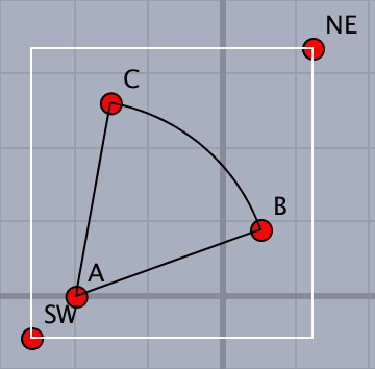
\includegraphics[bb=0.00 0.00 180.01 177.01,width=4cm"] {Fig/circledata3.pdf}\hspace{12mm}  %%% /Users/Hannya/Desktop/KeTCindy/fig/circledata2.tex 
%%% Generator=template1basic.cdy 
{\unitlength=1cm%
\begin{picture}%
(3.82,3.94)(-2.6,-0.57)%
\special{pn 8}%
%
{%
\color[rgb]{0,0,0}%
\special{pa   201  -357}\special{pa   193  -377}\special{pa   185  -398}\special{pa   176  -418}%
\special{pa   167  -438}\special{pa   158  -458}\special{pa   148  -478}\special{pa   138  -497}%
\special{pa   127  -516}\special{pa   116  -535}\special{pa   105  -554}\special{pa    93  -573}%
\special{pa    81  -591}\special{pa    68  -609}\special{pa    55  -627}\special{pa    42  -644}%
\special{pa    28  -662}\special{pa    14  -679}\special{pa    -0  -695}\special{pa   -15  -712}%
\special{pa   -30  -728}\special{pa   -45  -743}\special{pa   -61  -759}\special{pa   -77  -774}%
\special{pa   -93  -788}\special{pa  -110  -803}\special{pa  -127  -817}\special{pa  -144  -830}%
\special{pa  -162  -844}\special{pa  -180  -857}\special{pa  -198  -869}\special{pa  -216  -881}%
\special{pa  -235  -893}\special{pa  -253  -904}\special{pa  -272  -915}\special{pa  -292  -926}%
\special{pa  -311  -936}\special{pa  -331  -946}\special{pa  -351  -955}\special{pa  -371  -964}%
\special{pa  -391  -973}\special{pa  -412  -981}\special{pa  -432  -988}\special{pa  -453  -996}%
\special{pa  -474 -1002}\special{pa  -495 -1009}\special{pa  -516 -1015}\special{pa  -538 -1020}%
\special{pa  -559 -1025}\special{pa  -581 -1030}\special{pa  -602 -1034}%
\special{fp}%
}%
{%
\color[rgb]{0,0,0}%
\special{pa   201  -357}\special{pa  -787    -0}\special{pa  -602 -1034}%
\special{fp}%
}%
{%
\color[rgb]{0,0,0}%
\settowidth{\Width}{A}\setlength{\Width}{-0.5\Width}%
\settoheight{\Height}{A}\settodepth{\Depth}{A}\setlength{\Height}{-\Height}%
\put(-2.0000000,-0.0500000){\hspace*{\Width}\raisebox{\Height}{A}}%
%
}%
{%
\color[rgb]{0,0,0}%
\settowidth{\Width}{B}\setlength{\Width}{0\Width}%
\settoheight{\Height}{B}\settodepth{\Depth}{B}\setlength{\Height}{-0.5\Height}\setlength{\Depth}{0.5\Depth}\addtolength{\Height}{\Depth}%
\put(0.5600000,0.9100000){\hspace*{\Width}\raisebox{\Height}{B}}%
%
}%
{%
\color[rgb]{0,0,0}%
\settowidth{\Width}{C}\setlength{\Width}{-1\Width}%
\settoheight{\Height}{C}\settodepth{\Depth}{C}\setlength{\Height}{\Depth}%
\put(-1.5800000,2.6800000){\hspace*{\Width}\raisebox{\Height}{C}}%
%
}%
\end{picture}}%
\end{center}

1行目は,ABが$x$軸となす角を arctan2 関数 によって求めている。

\vspace{\baselineskip}
【例】弧を太く描く

    \verb|Circledata([C,D],["dr,3","Rng=[0,pi/3]"]);|

  円はNが大きな値の正N多角形として描いている。optionの ["Num=数値"] によってその細かさを指定できる。Nの値が小さければ正多角形が描けることになる。

\vspace{\baselineskip}
【例】A中心,半径ABの円と,その円に内接する正六角形
\begin{verbatim}
    Circledata("1",[A,B]);
    Circledata("2",[A,B],["Num=6"]);
\end{verbatim}
ここで,同じ[A,B]を使うため,nameを付与して区別する必要がある。(下図左)

また,頂点の位置を変えるのであれば,Rng= オプションを使う。(下図右)

 \verb|Circledata("2",[A,B],["Num=6","Rng=[pi/6,13/6*pi]"]);|

\hspace{10mm} %%% test.tex 2014-10-18 19:48
%%% test.sce 2014-10-18 19:48
{\unitlength=1cm%
\begin{picture}%
(   5.00000,   5.00000)(  -6.50000,  -1.50000)%
\special{pn 8}%
%
\special{pa -1566 -402}\special{pa -1573 -405}\special{pa -1580 -404}\special{pa -1585 -399}%
\special{pa -1586 -392}\special{pa -1583 -385}\special{pa -1577 -382}\special{pa -1569 -383}%
\special{pa -1564 -388}\special{pa -1563 -396}\special{pa -1566 -402}\special{sh 1}\special{fp}%
\special{pa -779 -402}\special{pa -786 -405}\special{pa -793 -404}\special{pa -798 -399}%
\special{pa -799 -392}\special{pa -796 -385}\special{pa -789 -382}\special{pa -782 -383}%
\special{pa -777 -388}\special{pa -776 -396}\special{pa -779 -402}\special{sh 1}\special{fp}%
\settowidth{\Width}{A}\setlength{\Width}{0\Width}%
\settoheight{\Height}{A}\settodepth{\Depth}{A}\setlength{\Height}{\Depth}%
\put(-3.9500,1.0500){\hspace*{\Width}\raisebox{\Height}{A}}%
%
%
\settowidth{\Width}{B}\setlength{\Width}{0\Width}%
\settoheight{\Height}{B}\settodepth{\Depth}{B}\setlength{\Height}{-0.5\Height}\setlength{\Depth}{0.5\Depth}\addtolength{\Height}{\Depth}%
\put(-1.9500,1.0000){\hspace*{\Width}\raisebox{\Height}{B}}%
%
%
\special{pa -787 -394}\special{pa -794 -492}\special{pa -812 -590}\special{pa -843 -684}%
\special{pa -885 -773}\special{pa -938 -857}\special{pa -1001 -933}\special{pa -1073 -1000}%
\special{pa -1153 -1059}\special{pa -1240 -1106}\special{pa -1331 -1143}\special{pa -1427 -1167}%
\special{pa -1525 -1180}\special{pa -1624 -1180}\special{pa -1722 -1167}\special{pa -1818 -1143}%
\special{pa -1910 -1106}\special{pa -1997 -1059}\special{pa -2077 -1000}\special{pa -2149 -933}%
\special{pa -2212 -857}\special{pa -2265 -773}\special{pa -2307 -684}\special{pa -2337 -590}%
\special{pa -2356 -492}\special{pa -2362 -394}\special{pa -2356 -295}\special{pa -2337 -198}%
\special{pa -2307 -104}\special{pa -2265 -14}\special{pa -2212 69}\special{pa -2149 145}%
\special{pa -2077 213}\special{pa -1997 271}\special{pa -1910 319}\special{pa -1818 355}%
\special{pa -1722 380}\special{pa -1624 392}\special{pa -1525 392}\special{pa -1427 380}%
\special{pa -1331 355}\special{pa -1240 319}\special{pa -1153 271}\special{pa -1073 213}%
\special{pa -1001 145}\special{pa -938 69}\special{pa -885 -14}\special{pa -843 -104}%
\special{pa -812 -198}\special{pa -794 -295}\special{pa -787 -394}%
\special{fp}%
\special{pa -787 -394}\special{pa -1181 -1076}\special{pa -1969 -1076}\special{pa -2362 -394}%
\special{pa -1969 288}\special{pa -1181 288}\special{pa -787 -394}%
\special{fp}%
\end{picture}}%
\hspace{5mm}  %%% /Users/Hannya/Desktop/KeTCindy/fig/circledata5.tex 
%%% Generator=template1basic.cdy 
{\unitlength=5mm%
\begin{picture}%
(8,8)(-4,-4)%
\special{pn 8}%
%
\special{pa   511  -295}\special{pa     0  -591}\special{pa  -511  -295}\special{pa  -511   295}%
\special{pa    -0   591}\special{pa   511   295}\special{pa   511  -295}%
\special{fp}%
\special{pn 1}%
{%
\color[rgb]{0,0,0}%
\special{pa 11 -11}\special{pa 0 -16}\special{pa -11 -11}\special{pa -16 0}\special{pa -11 11}\special{pa 0 16}\special{pa 11 11}\special{pa 16 0}\special{pa 11 -11}\special{sh 1}\special{fp}%
\special{pa 602 -11}\special{pa 591 -16}\special{pa 579 -11}\special{pa 575 0}\special{pa 579 11}\special{pa 591 16}\special{pa 602 11}\special{pa 606 0}\special{pa 602 -11}\special{sh 1}\special{fp}%
}%
\special{pn 8}%
\settowidth{\Width}{A}\setlength{\Width}{0\Width}%
\settoheight{\Height}{A}\settodepth{\Depth}{A}\setlength{\Height}{\Depth}%
\put(0.3000000,0.1000000){\hspace*{\Width}\raisebox{\Height}{A}}%
%
\settowidth{\Width}{B}\setlength{\Width}{0\Width}%
\settoheight{\Height}{B}\settodepth{\Depth}{B}\setlength{\Height}{-0.5\Height}\setlength{\Depth}{0.5\Depth}\addtolength{\Height}{\Depth}%
\put(3.3000000,0.0000000){\hspace*{\Width}\raisebox{\Height}{B}}%
%
\end{picture}}%

%\begin{flushright}  \hyperlink{functionlist}{$\Rightarrow$関数一覧}\end{flushright}

\vspace{\baselineskip}
\hypertarget{mkcircles}{}
\item[関数]  Mkcircles()
\item[機能]  すべての幾何円のPD を作成
\item[説明]  Cinderellaの「円を加える」ツール(3種類いずれでも)で描いたすべての円をそのままプロットデータとする。たとえば,中心A,円周上の点をBとした円を作ると,プロットデータcrABが作成される。その後,インスペクタで点Bの識別名を変更(たとえばQに)すると,プロットデータ名も変更される。円はすでに描かれていてもよい。

\vspace{\baselineskip}
\hypertarget{ellipseplot}{}
\item[関数]  Ellipseplot(name,点リスト ,定義域, options)
\item[機能]  焦点と通る点を与えて楕円を描く。
\item[説明]  点リストで2つの焦点と通る点を与える。点はCinderellaの幾何点が使える。

  また,通る点のかわりに,焦点からの距離の和を実数で与えることもできる。
  
  実際には,媒介変数表示$x=a \cos \theta,y=b \sin \theta$ を,回転・平行移動して描いている。定義域はこのときの$t$の定義域で,省略も可能。省略したときの初期値は[-5,5]

\vspace{\baselineskip}
【例】点A,Bを焦点とする楕円を描く。

\verb|Ellipseplot("1",[A,B,C]);|   点Cを通る楕円を描く。

\verb|Ellipseplot("1",[A,B,4]);|   焦点からの距離の和が4である楕円を描く。

\verb|Ellipseplot("1",[A,B,C],"[0,pi]");|   楕円の半分を描く。

\vspace{\baselineskip}
【例】Cinderellaの作図ツールを使う

作図ツールに,焦点と通る点で楕円を描くもの,点の極線を描くツールがある。(モードメニュー / 直線 / 点の極線)これを利用すると,楕円上にとった点をインシデントにできるので,インタラクティブに図を変更することができる。このCinderellaの作図機能と合わせて,一方の焦点から出た光が楕円上で反射して他方の焦点に至る,という図を次のようにして描くことができる。

まず,3つの点,焦点A,Bと通る点Cを適当な位置に作図する。次に「焦点と通る点で決まる楕円」ツールを選び,点A,B,Cを順に指定すると,楕円が描かれる。

モードメニューの「直線」から「点の極線」を選び,点Cと楕円を順に指定すると接線が引かれる。

「垂線を加える」ツールを用いて,点Cで垂線,すなわち法線を引く。(下図)

「点を加える」ツールを用いて,接線,法線上に適当に点を取る。(D,Eとなったとする)

次のスクリプトを書いて実行すると,楕円に関して入射角と反射角が等しくなるように光が反射する様子を図にすることができる。

\vspace{\baselineskip}
\begin{layer}{150}{0}
\putnotese{75}{5}{ 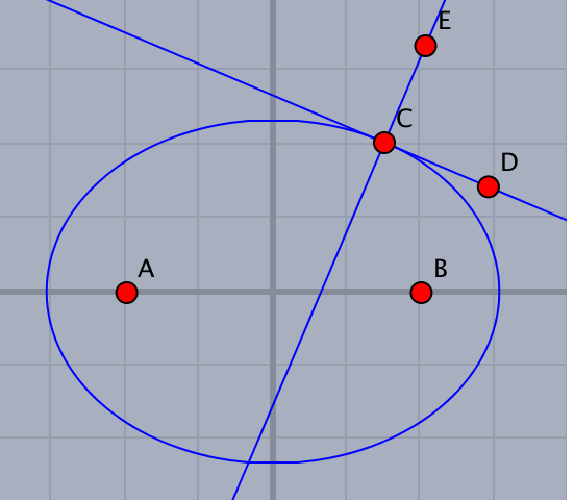
\includegraphics[bb=0 0 272.01 240.01, width=5cm]{Fig/ellipsecindy.pdf}}
\end{layer}
\hspace{50mm}

\begin{verbatim}
    Ellipseplot("1",[A,B,C]);
    Lineplot([C,D]);
    Lineplot([C,E]);
    Arrowdata([A,C]);
    Arrowdata([C,B]);
    Anglemark([A,C,B]);
    Expr([A,"s2","F_1",B,"s2","F_2"]);
\end{verbatim}
\vspace{\baselineskip}
    \begin{center} %%% fig.tex 2015-8-10 9:24
%%% fig.sce 2015-8-10 9:24
{\unitlength=8mm%
\begin{picture}%
(   7.62000,   5.82000)(  -3.62000,  -2.82000)%
\special{pn 8}%
%
\special{pa 915 0}\special{pa 908 -85}\special{pa 886 -169}\special{pa 849 -249}\special{pa 798 -326}%
\special{pa 734 -397}\special{pa 658 -462}\special{pa 571 -519}\special{pa 475 -568}%
\special{pa 371 -607}\special{pa 260 -637}\special{pa 146 -656}\special{pa 29 -664}%
\special{pa -88 -661}\special{pa -204 -648}\special{pa -316 -623}\special{pa -423 -589}%
\special{pa -524 -545}\special{pa -615 -492}\special{pa -697 -431}\special{pa -767 -362}%
\special{pa -825 -288}\special{pa -869 -209}\special{pa -899 -127}\special{pa -914 -43}%
\special{pa -914 43}\special{pa -899 127}\special{pa -869 209}\special{pa -825 288}%
\special{pa -767 362}\special{pa -697 431}\special{pa -615 492}\special{pa -524 545}%
\special{pa -423 589}\special{pa -316 623}\special{pa -204 648}\special{pa -88 661}%
\special{pa 29 664}\special{pa 146 656}\special{pa 260 637}\special{pa 371 607}\special{pa 475 568}%
\special{pa 571 519}\special{pa 658 462}\special{pa 734 397}\special{pa 798 326}\special{pa 849 249}%
\special{pa 886 169}\special{pa 908 85}\special{pa 915 0}%
\special{fp}%
\special{pa -59 888}\special{pa 290 -945}%
\special{fp}%
\special{pa -1140 -904}\special{pa 1260 -447}%
\special{fp}%
\special{pa -630 0}\special{pa 207 -624}%
\special{fp}%
\special{pa 187 -578}\special{pa 232 -643}\special{pa 158 -617}\special{pa 172 -598}%
\special{pa 187 -578}\special{sh 1}\special{ip}%
\special{pn 8}%
\special{pa 187 -578}\special{pa 232 -643}\special{pa 158 -617}\special{pa 172 -598}%
\special{pa 187 -578}%
\special{fp}%
\special{pn 8}%
\special{pa 232 -643}\special{pa 613 -27}%
\special{fp}%
\special{pa 570 -51}\special{pa 630 0}\special{pa 611 -76}\special{pa 591 -64}\special{pa 570 -51}%
\special{sh 1}\special{ip}%
\special{pn 8}%
\special{pa 570 -51}\special{pa 630 0}\special{pa 611 -76}\special{pa 591 -64}\special{pa 570 -51}%
\special{fp}%
\special{pn 8}%
\special{pa 106 -549}\special{pa 118 -535}\special{pa 132 -521}\special{pa 148 -510}%
\special{pa 165 -500}\special{pa 184 -493}\special{pa 203 -488}\special{pa 223 -485}%
\special{pa 242 -485}\special{pa 262 -488}\special{pa 281 -493}\special{pa 299 -500}%
\special{pa 315 -509}%
\special{fp}%
\settowidth{\Width}{$F_1$}\setlength{\Width}{-0.5\Width}%
\settoheight{\Height}{$F_1$}\settodepth{\Depth}{$F_1$}\setlength{\Height}{-\Height}%
\put(-2.0000,-0.1500){\hspace*{\Width}\raisebox{\Height}{$F_1$}}%
%
%
\settowidth{\Width}{$F_2$}\setlength{\Width}{-0.5\Width}%
\settoheight{\Height}{$F_2$}\settodepth{\Depth}{$F_2$}\setlength{\Height}{-\Height}%
\put(2.0000,-0.1500){\hspace*{\Width}\raisebox{\Height}{$F_2$}}%
%
%
\special{pn 8}%
\special{pa -1140 0}\special{pa 1260 0}%
\special{fp}%
\special{pn 8}%
\special{pa 1185 24}\special{pa 1260 0}\special{pa 1185 -24}\special{pa 1185 0}\special{pa 1185 24}%
\special{sh 1}\special{ip}%
\special{pn 8}%
\special{pa 1185 24}\special{pa 1260 0}\special{pa 1185 -24}\special{pa 1185 0}\special{pa 1185 24}%
\special{fp}%
\special{pn 8}%
\special{pn 8}%
\special{pa 0 888}\special{pa 0 -945}%
\special{fp}%
\special{pn 8}%
\special{pa 24 -870}\special{pa 0 -945}\special{pa -24 -870}\special{pa 0 -870}\special{pa 24 -870}%
\special{sh 1}\special{ip}%
\special{pn 8}%
\special{pa 24 -870}\special{pa 0 -945}\special{pa -24 -870}\special{pa 0 -870}\special{pa 24 -870}%
\special{fp}%
\special{pn 8}%
\settowidth{\Width}{$x$}\setlength{\Width}{0\Width}%
\settoheight{\Height}{$x$}\settodepth{\Depth}{$x$}\setlength{\Height}{-0.5\Height}\setlength{\Depth}{0.5\Depth}\addtolength{\Height}{\Depth}%
\put(4.0500,0.0000){\hspace*{\Width}\raisebox{\Height}{$x$}}%
%
%
\settowidth{\Width}{$y$}\setlength{\Width}{-0.5\Width}%
\settoheight{\Height}{$y$}\settodepth{\Depth}{$y$}\setlength{\Height}{\Depth}%
\put(0.0000,3.0500){\hspace*{\Width}\raisebox{\Height}{$y$}}%
%
%
\settowidth{\Width}{O}\setlength{\Width}{-1\Width}%
\settoheight{\Height}{O}\settodepth{\Depth}{O}\setlength{\Height}{-\Height}%
\put(-0.0500,-0.0500){\hspace*{\Width}\raisebox{\Height}{O}}%
%
%
\end{picture}}%\end{center}

  また,接線,法線を描かず,この楕円上に点D,E,・・をとり(個数は任意)次のスクリプトを書けば,何本かの光線が一方の焦点を出て他方の焦点に集まる様子を描くことができる。
  
\begin{layer}{150}{0}
    \putnotese{70}{0}{\scalebox{0.9}{ %%% fig.tex 2015-8-10 9:41
%%% fig.sce 2015-8-10 9:41
{\unitlength=8mm%
\begin{picture}%
(   7.62000,   5.82000)(  -3.62000,  -2.82000)%
\special{pn 8}%
%
\special{pa 915 0}\special{pa 908 -85}\special{pa 886 -169}\special{pa 849 -249}\special{pa 798 -326}%
\special{pa 734 -397}\special{pa 658 -462}\special{pa 571 -519}\special{pa 475 -568}%
\special{pa 371 -607}\special{pa 260 -637}\special{pa 146 -656}\special{pa 29 -664}%
\special{pa -88 -661}\special{pa -204 -648}\special{pa -316 -623}\special{pa -423 -589}%
\special{pa -524 -545}\special{pa -615 -492}\special{pa -697 -431}\special{pa -767 -362}%
\special{pa -825 -288}\special{pa -869 -209}\special{pa -899 -127}\special{pa -914 -43}%
\special{pa -914 43}\special{pa -899 127}\special{pa -869 209}\special{pa -825 288}%
\special{pa -767 362}\special{pa -697 431}\special{pa -615 492}\special{pa -524 545}%
\special{pa -423 589}\special{pa -316 623}\special{pa -204 648}\special{pa -88 661}%
\special{pa 29 664}\special{pa 146 656}\special{pa 260 637}\special{pa 371 607}\special{pa 475 568}%
\special{pa 571 519}\special{pa 658 462}\special{pa 734 397}\special{pa 798 326}\special{pa 849 249}%
\special{pa 886 169}\special{pa 908 85}\special{pa 915 0}%
\special{fp}%
\special{pa -630 0}\special{pa 232 -643}\special{pa 630 0}%
\special{fp}%
\special{pa -630 0}\special{pa -430 -586}\special{pa 630 0}%
\special{fp}%
\special{pa -630 0}\special{pa 694 -433}\special{pa 630 0}%
\special{fp}%
\settowidth{\Width}{$F_1$}\setlength{\Width}{-0.5\Width}%
\settoheight{\Height}{$F_1$}\settodepth{\Depth}{$F_1$}\setlength{\Height}{-\Height}%
\put(-2.0000,-0.1500){\hspace*{\Width}\raisebox{\Height}{$F_1$}}%
%
%
\settowidth{\Width}{$F_2$}\setlength{\Width}{-0.5\Width}%
\settoheight{\Height}{$F_2$}\settodepth{\Depth}{$F_2$}\setlength{\Height}{-\Height}%
\put(2.0000,-0.1500){\hspace*{\Width}\raisebox{\Height}{$F_2$}}%
%
%
\special{pn 8}%
\special{pa -1140 0}\special{pa 1260 0}%
\special{fp}%
\special{pn 8}%
\special{pa 1185 24}\special{pa 1260 0}\special{pa 1185 -24}\special{pa 1185 0}\special{pa 1185 24}%
\special{sh 1}\special{ip}%
\special{pn 8}%
\special{pa 1185 24}\special{pa 1260 0}\special{pa 1185 -24}\special{pa 1185 0}\special{pa 1185 24}%
\special{fp}%
\special{pn 8}%
\special{pn 8}%
\special{pa 0 888}\special{pa 0 -945}%
\special{fp}%
\special{pn 8}%
\special{pa 24 -870}\special{pa 0 -945}\special{pa -24 -870}\special{pa 0 -870}\special{pa 24 -870}%
\special{sh 1}\special{ip}%
\special{pn 8}%
\special{pa 24 -870}\special{pa 0 -945}\special{pa -24 -870}\special{pa 0 -870}\special{pa 24 -870}%
\special{fp}%
\special{pn 8}%
\settowidth{\Width}{$x$}\setlength{\Width}{0\Width}%
\settoheight{\Height}{$x$}\settodepth{\Depth}{$x$}\setlength{\Height}{-0.5\Height}\setlength{\Depth}{0.5\Depth}\addtolength{\Height}{\Depth}%
\put(4.0500,0.0000){\hspace*{\Width}\raisebox{\Height}{$x$}}%
%
%
\settowidth{\Width}{$y$}\setlength{\Width}{-0.5\Width}%
\settoheight{\Height}{$y$}\settodepth{\Depth}{$y$}\setlength{\Height}{\Depth}%
\put(0.0000,3.0500){\hspace*{\Width}\raisebox{\Height}{$y$}}%
%
%
\settowidth{\Width}{O}\setlength{\Width}{-1\Width}%
\settoheight{\Height}{O}\settodepth{\Depth}{O}\setlength{\Height}{-\Height}%
\put(-0.0500,-0.0500){\hspace*{\Width}\raisebox{\Height}{O}}%
%
%
\end{picture}}%}}
\end{layer}
\begin{verbatim}
    Ellipseplot("1",[A,B,C]);
    Listplot([A,C,B]);
    Listplot([A,D,B]);
    Listplot([A,E,B]);
    Expr([A,"s2","F_1",B,"s2","F_2"]);
\end{verbatim}

\vspace{10mm}

\hypertarget{hyperbolaplot}{}
\item[関数]  Hyperbolaplot(name,点リスト ,定義域, options)
\item[機能]  焦点と通る点を与えて双曲線を描く。
\item[説明]  点リストで2つの焦点と通る点を与える。点はCinderellaの幾何点が使える。

また,通る点のかわりに,焦点からの距離の差を実数で与えることもできる。

実際には,ハイパボリック関数を用いた媒介変数表示 $x=\cosh t,y=\sinh t$を回転・平行移動している。

optionとして,"Asy=線種"  を与えると,漸近線を指定した線種で表示する。 初期設定では漸近線は非表示。
  
\vspace{\baselineskip}
【例】点A,Bを焦点とする双曲線を描く。

\verb|Hyperbolaplot("1",[A,B,C]);|     点Cを通る双曲線を描く。

\verb|Hyperbolaplot("1",[A,B,2]);|      焦点からの距離の差が2の双曲線を描く。

\verb|Hyperbolaplot("1",[A,B,C],["Asy=do"]);|   漸近線を点線で描く。

\vspace{\baselineskip}
\hspace{20mm} \scalebox{0.9}{%%% fig.tex 2015-8-10 11:14
%%% fig.sce 2015-8-10 11:14
{\unitlength=8mm%
\begin{picture}%
(   7.00000,   5.00000)(  -3.50000,  -2.50000)%
\special{pn 8}%
%
\special{pa 908 787}\special{pa 862 734}\special{pa 791 650}\special{pa 728 573}\special{pa 673 502}%
\special{pa 625 436}\special{pa 584 374}\special{pa 548 317}\special{pa 519 263}\special{pa 494 211}%
\special{pa 475 162}\special{pa 461 115}\special{pa 452 68}\special{pa 447 23}\special{pa 447 -23}%
\special{pa 452 -68}\special{pa 461 -115}\special{pa 475 -162}\special{pa 494 -211}%
\special{pa 519 -263}\special{pa 548 -317}\special{pa 584 -374}\special{pa 625 -436}%
\special{pa 673 -502}\special{pa 728 -573}\special{pa 791 -650}\special{pa 862 -734}%
\special{pa 908 -787}%
\special{fp}%
\special{pa -908 787}\special{pa -862 734}\special{pa -791 650}\special{pa -728 573}%
\special{pa -673 502}\special{pa -625 436}\special{pa -584 374}\special{pa -548 317}%
\special{pa -519 263}\special{pa -494 211}\special{pa -475 162}\special{pa -461 115}%
\special{pa -452 68}\special{pa -447 23}\special{pa -447 -23}\special{pa -452 -68}%
\special{pa -461 -115}\special{pa -475 -162}\special{pa -494 -211}\special{pa -519 -263}%
\special{pa -548 -317}\special{pa -584 -374}\special{pa -625 -436}\special{pa -673 -502}%
\special{pa -728 -573}\special{pa -791 -650}\special{pa -862 -734}\special{pa -908 -787}%
\special{fp}%
\special{pn 8}%
\special{pa 796 -790}\special{pa 790 -785}\special{fp}\special{pa 768 -763}\special{pa 762 -757}\special{fp}%
\special{pa 740 -735}\special{pa 734 -729}\special{fp}\special{pa 712 -707}\special{pa 707 -702}\special{fp}%
\special{pa 685 -680}\special{pa 679 -674}\special{fp}\special{pa 657 -652}\special{pa 651 -646}\special{fp}%
\special{pa 629 -624}\special{pa 623 -619}\special{fp}\special{pa 601 -597}\special{pa 595 -591}\special{fp}%
\special{pa 573 -569}\special{pa 568 -564}\special{fp}\special{pa 545 -542}\special{pa 540 -536}\special{fp}%
\special{pa 518 -514}\special{pa 512 -508}\special{fp}\special{pa 490 -486}\special{pa 484 -481}\special{fp}%
\special{pa 462 -459}\special{pa 456 -453}\special{fp}\special{pa 434 -431}\special{pa 428 -425}\special{fp}%
\special{pa 406 -403}\special{pa 401 -398}\special{fp}\special{pa 378 -376}\special{pa 373 -370}\special{fp}%
\special{pa 351 -348}\special{pa 345 -343}\special{fp}\special{pa 323 -321}\special{pa 317 -315}\special{fp}%
\special{pa 295 -293}\special{pa 289 -287}\special{fp}\special{pa 267 -265}\special{pa 261 -260}\special{fp}%
\special{pa 239 -238}\special{pa 234 -232}\special{fp}\special{pa 212 -210}\special{pa 206 -204}\special{fp}%
\special{pa 184 -182}\special{pa 178 -177}\special{fp}\special{pa 156 -155}\special{pa 150 -149}\special{fp}%
\special{pa 128 -127}\special{pa 122 -122}\special{fp}\special{pa 100 -100}\special{pa 95 -94}\special{fp}%
\special{pa 72 -72}\special{pa 67 -66}\special{fp}\special{pa 45 -44}\special{pa 39 -39}\special{fp}%
\special{pa 17 -17}\special{pa 11 -11}\special{fp}\special{pa -11 11}\special{pa -17 17}\special{fp}%
\special{pa -39 39}\special{pa -45 44}\special{fp}\special{pa -67 66}\special{pa -72 72}\special{fp}%
\special{pa -95 94}\special{pa -100 100}\special{fp}\special{pa -122 122}\special{pa -128 127}\special{fp}%
\special{pa -150 149}\special{pa -156 155}\special{fp}\special{pa -178 177}\special{pa -184 182}\special{fp}%
\special{pa -206 204}\special{pa -212 210}\special{fp}\special{pa -234 232}\special{pa -239 238}\special{fp}%
\special{pa -261 260}\special{pa -267 265}\special{fp}\special{pa -289 287}\special{pa -295 293}\special{fp}%
\special{pa -317 315}\special{pa -323 321}\special{fp}\special{pa -345 343}\special{pa -351 348}\special{fp}%
\special{pa -373 370}\special{pa -378 376}\special{fp}\special{pa -401 398}\special{pa -406 403}\special{fp}%
\special{pa -428 425}\special{pa -434 431}\special{fp}\special{pa -456 453}\special{pa -462 459}\special{fp}%
\special{pa -484 481}\special{pa -490 486}\special{fp}\special{pa -512 508}\special{pa -518 514}\special{fp}%
\special{pa -540 536}\special{pa -545 542}\special{fp}\special{pa -568 564}\special{pa -573 569}\special{fp}%
\special{pa -595 591}\special{pa -601 597}\special{fp}\special{pa -623 619}\special{pa -629 624}\special{fp}%
\special{pa -651 646}\special{pa -657 652}\special{fp}\special{pa -679 674}\special{pa -685 680}\special{fp}%
\special{pa -707 702}\special{pa -712 707}\special{fp}\special{pa -734 729}\special{pa -740 735}\special{fp}%
\special{pa -762 757}\special{pa -768 763}\special{fp}\special{pa -790 785}\special{pa -796 790}\special{fp}%
\special{pn 8}%
\special{pa -796 -790}\special{pa -790 -785}\special{fp}\special{pa -768 -763}\special{pa -762 -757}\special{fp}%
\special{pa -740 -735}\special{pa -734 -729}\special{fp}\special{pa -712 -707}\special{pa -707 -702}\special{fp}%
\special{pa -685 -680}\special{pa -679 -674}\special{fp}\special{pa -657 -652}\special{pa -651 -646}\special{fp}%
\special{pa -629 -624}\special{pa -623 -619}\special{fp}\special{pa -601 -597}\special{pa -595 -591}\special{fp}%
\special{pa -573 -569}\special{pa -568 -564}\special{fp}\special{pa -545 -542}\special{pa -540 -536}\special{fp}%
\special{pa -518 -514}\special{pa -512 -508}\special{fp}\special{pa -490 -486}\special{pa -484 -481}\special{fp}%
\special{pa -462 -459}\special{pa -456 -453}\special{fp}\special{pa -434 -431}\special{pa -428 -425}\special{fp}%
\special{pa -406 -403}\special{pa -401 -398}\special{fp}\special{pa -378 -376}\special{pa -373 -370}\special{fp}%
\special{pa -351 -348}\special{pa -345 -343}\special{fp}\special{pa -323 -321}\special{pa -317 -315}\special{fp}%
\special{pa -295 -293}\special{pa -289 -287}\special{fp}\special{pa -267 -265}\special{pa -261 -260}\special{fp}%
\special{pa -239 -238}\special{pa -234 -232}\special{fp}\special{pa -212 -210}\special{pa -206 -204}\special{fp}%
\special{pa -184 -182}\special{pa -178 -177}\special{fp}\special{pa -156 -155}\special{pa -150 -149}\special{fp}%
\special{pa -128 -127}\special{pa -122 -122}\special{fp}\special{pa -100 -100}\special{pa -95 -94}\special{fp}%
\special{pa -72 -72}\special{pa -67 -66}\special{fp}\special{pa -45 -44}\special{pa -39 -39}\special{fp}%
\special{pa -17 -17}\special{pa -11 -11}\special{fp}\special{pa 11 11}\special{pa 17 17}\special{fp}%
\special{pa 39 39}\special{pa 45 44}\special{fp}\special{pa 67 66}\special{pa 72 72}\special{fp}%
\special{pa 95 94}\special{pa 100 100}\special{fp}\special{pa 122 122}\special{pa 128 127}\special{fp}%
\special{pa 150 149}\special{pa 156 155}\special{fp}\special{pa 178 177}\special{pa 184 182}\special{fp}%
\special{pa 206 204}\special{pa 212 210}\special{fp}\special{pa 234 232}\special{pa 239 238}\special{fp}%
\special{pa 261 260}\special{pa 267 265}\special{fp}\special{pa 289 287}\special{pa 295 293}\special{fp}%
\special{pa 317 315}\special{pa 323 321}\special{fp}\special{pa 345 343}\special{pa 351 348}\special{fp}%
\special{pa 373 370}\special{pa 378 376}\special{fp}\special{pa 401 398}\special{pa 406 403}\special{fp}%
\special{pa 428 425}\special{pa 434 431}\special{fp}\special{pa 456 453}\special{pa 462 459}\special{fp}%
\special{pa 484 481}\special{pa 490 486}\special{fp}\special{pa 512 508}\special{pa 518 514}\special{fp}%
\special{pa 540 536}\special{pa 545 542}\special{fp}\special{pa 568 564}\special{pa 573 569}\special{fp}%
\special{pa 595 591}\special{pa 601 597}\special{fp}\special{pa 623 619}\special{pa 629 624}\special{fp}%
\special{pa 651 646}\special{pa 657 652}\special{fp}\special{pa 679 674}\special{pa 685 680}\special{fp}%
\special{pa 707 702}\special{pa 712 707}\special{fp}\special{pa 734 729}\special{pa 740 735}\special{fp}%
\special{pa 762 757}\special{pa 768 763}\special{fp}\special{pa 790 785}\special{pa 796 790}\special{fp}%
\special{pn 8}%
\special{pa -619 -11}\special{pa -626 -15}\special{pa -634 -15}\special{pa -641 -11}%
\special{pa -645 -4}\special{pa -645 4}\special{pa -641 11}\special{pa -634 15}\special{pa -626 15}%
\special{pa -619 11}\special{pa -615 4}\special{pa -615 -4}\special{pa -619 -11}\special{sh 1}\special{fp}%
\special{pa 641 -11}\special{pa 634 -15}\special{pa 626 -15}\special{pa 619 -11}\special{pa 615 -4}%
\special{pa 615 4}\special{pa 619 11}\special{pa 626 15}\special{pa 634 15}\special{pa 641 11}%
\special{pa 645 4}\special{pa 645 -4}\special{pa 641 -11}\special{sh 1}\special{fp}%
\special{pa 579 -360}\special{pa 571 -364}\special{pa 563 -364}\special{pa 556 -360}%
\special{pa 552 -353}\special{pa 552 -345}\special{pa 556 -337}\special{pa 563 -333}%
\special{pa 571 -333}\special{pa 579 -337}\special{pa 583 -345}\special{pa 583 -353}%
\special{pa 579 -360}\special{sh 1}\special{fp}%
\settowidth{\Width}{A}\setlength{\Width}{-0.5\Width}%
\settoheight{\Height}{A}\settodepth{\Depth}{A}\setlength{\Height}{-\Height}%
\put(-2.0000,-0.1500){\hspace*{\Width}\raisebox{\Height}{A}}%
%
%
\settowidth{\Width}{B}\setlength{\Width}{-0.5\Width}%
\settoheight{\Height}{B}\settodepth{\Depth}{B}\setlength{\Height}{-\Height}%
\put(2.0000,-0.1500){\hspace*{\Width}\raisebox{\Height}{B}}%
%
%
\settowidth{\Width}{C}\setlength{\Width}{0\Width}%
\settoheight{\Height}{C}\settodepth{\Depth}{C}\setlength{\Height}{-0.5\Height}\setlength{\Depth}{0.5\Depth}\addtolength{\Height}{\Depth}%
\put(1.9514,1.1069){\hspace*{\Width}\raisebox{\Height}{C}}%
%
%
\special{pn 8}%
\special{pa -1102 0}\special{pa 1102 0}%
\special{fp}%
\special{pn 8}%
\special{pa 1027 24}\special{pa 1102 0}\special{pa 1027 -24}\special{pa 1027 0}\special{pa 1027 24}%
\special{sh 1}\special{ip}%
\special{pn 8}%
\special{pa 1027 24}\special{pa 1102 0}\special{pa 1027 -24}\special{pa 1027 0}\special{pa 1027 24}%
\special{fp}%
\special{pn 8}%
\special{pn 8}%
\special{pa 0 787}\special{pa 0 -787}%
\special{fp}%
\special{pn 8}%
\special{pa 24 -713}\special{pa 0 -787}\special{pa -24 -713}\special{pa 0 -713}\special{pa 24 -713}%
\special{sh 1}\special{ip}%
\special{pn 8}%
\special{pa 24 -713}\special{pa 0 -787}\special{pa -24 -713}\special{pa 0 -713}\special{pa 24 -713}%
\special{fp}%
\special{pn 8}%
\settowidth{\Width}{$x$}\setlength{\Width}{0\Width}%
\settoheight{\Height}{$x$}\settodepth{\Depth}{$x$}\setlength{\Height}{-0.5\Height}\setlength{\Depth}{0.5\Depth}\addtolength{\Height}{\Depth}%
\put(3.5500,0.0000){\hspace*{\Width}\raisebox{\Height}{$x$}}%
%
%
\settowidth{\Width}{$y$}\setlength{\Width}{-0.5\Width}%
\settoheight{\Height}{$y$}\settodepth{\Depth}{$y$}\setlength{\Height}{\Depth}%
\put(0.0000,2.5500){\hspace*{\Width}\raisebox{\Height}{$y$}}%
%
%
\settowidth{\Width}{O}\setlength{\Width}{-1\Width}%
\settoheight{\Height}{O}\settodepth{\Depth}{O}\setlength{\Height}{-\Height}%
\put(-0.0500,-0.0500){\hspace*{\Width}\raisebox{\Height}{O}}%
%
%
\end{picture}}%}
\begin{flushright}  \hyperlink{functionlist}{$\Rightarrow$関数一覧}\end{flushright}

\vspace{\baselineskip}
\hypertarget{parabolaplot}{}
\item[関数]  Parabolaplot(name,点リスト ,定義域, options)
\item[機能]  点リスト[A,B,C]で示された焦点,準線で決まる放物線を描く。
\item[説明]  焦点Aと準線BCで決定する放物線を描く。

  実際には,2次関数 $y=x^2$のグラフを回転・平行移動して描いており,定義域は,$y=x^2$での定義域と考えてよい。定義域は省略することもできる。省略したときの初期値は[-5,5]

\vspace{\baselineskip}
【例】点Aを焦点,直線BCを準線とする放物線を描く

\hspace{10mm}\verb|Parabolaplot("1",[A,B,C]); |
      
定義域を $-4 \leq x \leq 4$ とする。

\hspace{10mm} \verb|Parabolaplot("1",[A,B,C],"[-4,4]");|

点(0,1)を焦点,直線$y=-1$を準線とする放物線を描く

\hspace{10mm} \verb|Parabolaplot("1",[[0,1],[-1,-1],[1,-1]]);|

\vspace{\baselineskip}
【例】放物線上の2点で引かれた接線と放物線で囲まれた領域を斜線で描く。

Cinderellaの作図ツールに,焦点と準線で放物線を描くものがある。また,点の極線を描くツールがある。(モードメニュー / 直線 / 点の極線)これを利用すると,放物線上にとった点をインシデントにできるので,インタラクティブに図を変更することができる。このCinderellaの作図機能と合わせて,次の手順で図を描く。
  
まず,焦点A(0,1)と準線$y=-1$:BCを作図する。次に「焦点と準線で決まる放物線」ツールを選び,点Aと直線BCを指定すると,放物線が描かれる。方程式では$y=\dfrac{1}{4}x^2$の放物線である。

次に,放物線上に点D,Eをとる。Cinderellaの作図機能を用いているので,この2点は放物線上だけを動かすことができる。(インシデント)

モードメニューの「直線」から「点の極線」を選び,点Dと放物線,点Eと放物線を順に指定すると接線が引かれる。その交点に点を取る。

\vspace{\baselineskip}
\begin{center} 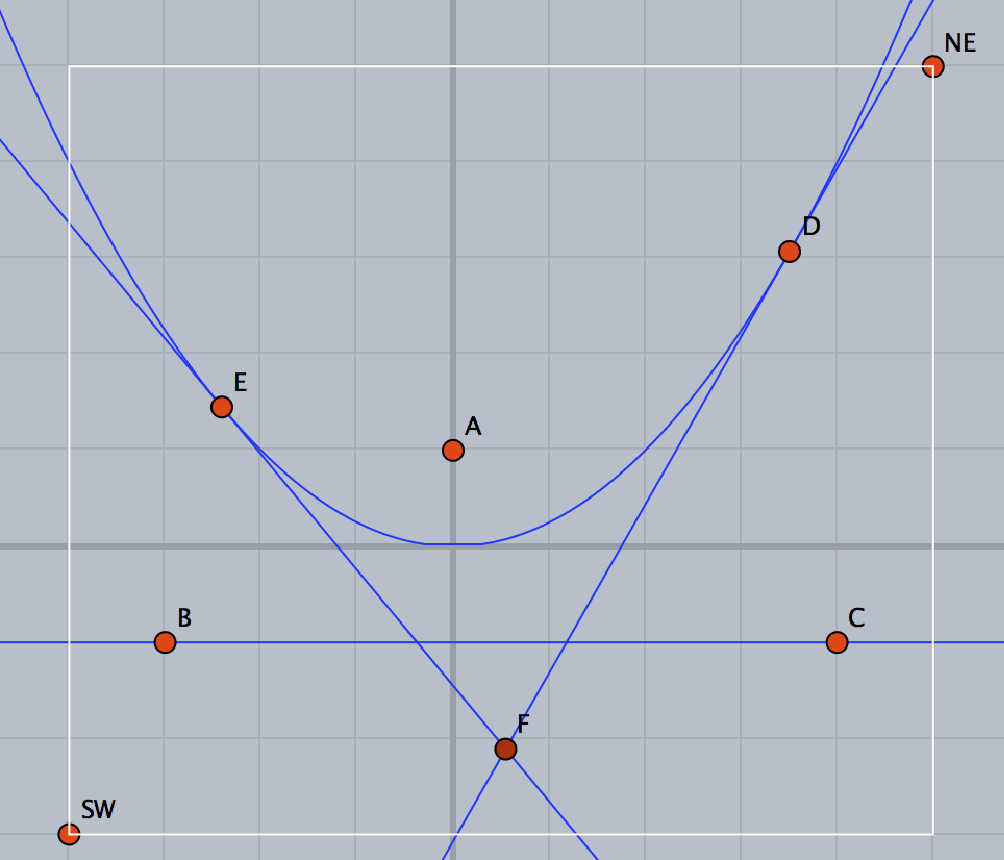
\includegraphics[bb=0 0 482.02 413.02 , width=6cm]{Fig/parabolaplot.pdf} \end{center}
            
\vspace{\baselineskip}
  以上で作図ができたので,次のスクリプトを書いて実行する。
\begin{verbatim}
  Parabolaplot("1",[A,B,C]);
  Lineplot([D,F]);
  Lineplot([E,F]);
  Hatchdata("1",["iii"],[["gr1para","s"],["lnEF","n"],["lnDF","n"]]);
\end{verbatim}

これで,次図ができる。このあと,文字などは適当に追加する。
 
\vspace{\baselineskip}
\begin{center} %%% fig.tex 2015-8-3 20:14
%%% fig.sce 2015-8-3 20:14
{\unitlength=4mm%
\begin{picture}%
(   9.00000,   8.00000)(  -4.00000,  -3.00000)%
\special{pn 8}%
%
\special{pa -630 -630}\special{pa -627 -624}\special{pa -595 -561}\special{pa -562 -502}%
\special{pa -530 -446}\special{pa -498 -394}\special{pa -466 -345}\special{pa -434 -299}%
\special{pa -402 -256}\special{pa -370 -217}\special{pa -337 -181}\special{pa -305 -148}%
\special{pa -273 -118}\special{pa -241 -92}\special{pa -209 -69}\special{pa -177 -50}%
\special{pa -145 -33}\special{pa -112 -20}\special{pa -80 -10}\special{pa -48 -4}%
\special{pa -16 0}\special{pa 16 0}\special{pa 48 -4}\special{pa 80 -10}\special{pa 112 -20}%
\special{pa 145 -33}\special{pa 177 -50}\special{pa 209 -69}\special{pa 241 -92}\special{pa 273 -118}%
\special{pa 305 -148}\special{pa 337 -181}\special{pa 370 -217}\special{pa 402 -256}%
\special{pa 434 -299}\special{pa 466 -345}\special{pa 498 -394}\special{pa 530 -446}%
\special{pa 562 -502}\special{pa 595 -561}\special{pa 627 -624}\special{pa 659 -689}%
\special{pa 691 -758}\special{pa 704 -787}%
\special{fp}%
\special{pa 725 -787}\special{pa 6 472}%
\special{fp}%
\special{pa -630 -530}\special{pa 202 472}%
\special{fp}%
\special{pa -379 -229}\special{pa 86 333}\special{pa 552 -484}%
\special{fp}%
\special{pa 75 319}\special{pa 119 276}%
\special{fp}%
\special{pa 63 304}\special{pa 156 211}%
\special{fp}%
\special{pa 50 289}\special{pa 193 146}%
\special{fp}%
\special{pa 37 274}\special{pa 229 82}%
\special{fp}%
\special{pa 25 258}\special{pa 266 17}%
\special{fp}%
\special{pa 12 243}\special{pa 303 -48}%
\special{fp}%
\special{pa -1 228}\special{pa 340 -113}%
\special{fp}%
\special{pa -13 213}\special{pa 377 -178}%
\special{fp}%
\special{pa -26 198}\special{pa 414 -243}%
\special{fp}%
\special{pa -38 182}\special{pa 224 -80}%
\special{fp}%
\special{pa 407 -263}\special{pa 451 -307}%
\special{fp}%
\special{pa -51 167}\special{pa 154 -38}%
\special{fp}%
\special{pa 476 -360}\special{pa 488 -372}%
\special{fp}%
\special{pa -64 152}\special{pa 107 -18}%
\special{fp}%
\special{pa 523 -435}\special{pa 525 -437}%
\special{fp}%
\special{pa -76 137}\special{pa 68 -8}%
\special{fp}%
\special{pa -89 121}\special{pa 35 -2}%
\special{fp}%
\special{pa -102 106}\special{pa 5 0}%
\special{fp}%
\special{pa -114 91}\special{pa -22 -1}%
\special{fp}%
\special{pa -127 76}\special{pa -47 -4}%
\special{fp}%
\special{pa -139 61}\special{pa -71 -8}%
\special{fp}%
\special{pa -152 45}\special{pa -93 -14}%
\special{fp}%
\special{pa -165 30}\special{pa -114 -21}%
\special{fp}%
\special{pa -177 15}\special{pa -134 -29}%
\special{fp}%
\special{pa -190 0}\special{pa -153 -37}%
\special{fp}%
\special{pa -203 -15}\special{pa -171 -47}%
\special{fp}%
\special{pa -215 -31}\special{pa -189 -57}%
\special{fp}%
\special{pa -228 -46}\special{pa -206 -68}%
\special{fp}%
\special{pa -240 -61}\special{pa -222 -79}%
\special{fp}%
\special{pa -253 -76}\special{pa -239 -91}%
\special{fp}%
\special{pa -266 -91}\special{pa -254 -103}%
\special{fp}%
\special{pa -278 -107}\special{pa -269 -115}%
\special{fp}%
\special{pa -291 -122}\special{pa -284 -129}%
\special{fp}%
\special{pa -304 -137}\special{pa -299 -142}%
\special{fp}%
\special{pa -316 -152}\special{pa -313 -156}%
\special{fp}%
\special{pa -329 -168}\special{pa -327 -170}%
\special{fp}%
\special{pa -341 -183}\special{pa -340 -184}%
\special{fp}%
\special{pa -354 -198}\special{pa -353 -199}%
\special{fp}%
\special{pa -367 -213}\special{pa -366 -213}%
\special{fp}%
\special{pa -379 -228}\special{pa -379 -229}%
\special{fp}%
\special{pn 8}%
\special{pa -630 0}\special{pa 787 0}%
\special{fp}%
\special{pn 8}%
\special{pa 713 24}\special{pa 787 0}\special{pa 713 -24}\special{pa 713 0}\special{pa 713 24}%
\special{sh 1}\special{ip}%
\special{pn 8}%
\special{pa 713 24}\special{pa 787 0}\special{pa 713 -24}\special{pa 713 0}\special{pa 713 24}%
\special{fp}%
\special{pn 8}%
\special{pn 8}%
\special{pa 0 472}\special{pa 0 -787}%
\special{fp}%
\special{pn 8}%
\special{pa 24 -713}\special{pa 0 -787}\special{pa -24 -713}\special{pa 0 -713}\special{pa 24 -713}%
\special{sh 1}\special{ip}%
\special{pn 8}%
\special{pa 24 -713}\special{pa 0 -787}\special{pa -24 -713}\special{pa 0 -713}\special{pa 24 -713}%
\special{fp}%
\special{pn 8}%
\settowidth{\Width}{$x$}\setlength{\Width}{0\Width}%
\settoheight{\Height}{$x$}\settodepth{\Depth}{$x$}\setlength{\Height}{-0.5\Height}\setlength{\Depth}{0.5\Depth}\addtolength{\Height}{\Depth}%
\put(5.0500,0.0000){\hspace*{\Width}\raisebox{\Height}{$x$}}%
%
%
\settowidth{\Width}{$y$}\setlength{\Width}{-0.5\Width}%
\settoheight{\Height}{$y$}\settodepth{\Depth}{$y$}\setlength{\Height}{\Depth}%
\put(0.0000,5.0500){\hspace*{\Width}\raisebox{\Height}{$y$}}%
%
%
\settowidth{\Width}{O}\setlength{\Width}{-1\Width}%
\settoheight{\Height}{O}\settodepth{\Depth}{O}\setlength{\Height}{-\Height}%
\put(-0.0500,-0.0500){\hspace*{\Width}\raisebox{\Height}{O}}%
%
%
\end{picture}}%\end{center}

なお,Cinderellaの作図ツールで放物線を描かず,焦点Aと準線上の点B,Cだけを用意して,次のスクリプトで描くこともできる。
\begin{verbatim}
  Parabolaplot("1",[A,B,C]);
  Putoncurve("D","gr1para");
  Putoncurve("E","gr1para");
  Tangentplot("1","gr1para","x="+D.x);
  Tangentplot("2","gr1para","x="+E.x);
  Hatchdata("1",["iii"],[["gr1para","s"],["lntn1","n"],["lntn2","n"]]);
\end{verbatim}

\begin{flushright}  \hyperlink{functionlist}{$\Rightarrow$関数一覧}\end{flushright}

%\vspace{\baselineskip}
\hypertarget{ovaldata}{}
\item[関数]  Ovaldata(name, 点リスト,options)
\item[機能]  角を丸くした矩形を描く
\item[説明]  中心と対角の1点を指定し,角を丸くした矩形を描く

optionsは,角の落とし具合と線種など。 初期設定は0.2 

\vspace{\baselineskip}
【例】いくつかの例を示す。
\begin{verbatim}
    Ovaldata("1", [A,B]);
    Ovaldata("2", [C,D],[0]);
    Ovaldata("3", [E,F],[1,"dr,3"]);
    Ovaldata("4", [G,H],[1.5,"da"]);
\end{verbatim}
\begin{center} %%% test.tex 2014-11-30 22:38
%%% test.sce 2014-11-30 22:38
{\unitlength=5mm%
\begin{picture}%
(  21.04000,   5.44000)(  -3.04000,   0.56000)%
\special{pn 8}%
%
\special{pn 24}%
\special{pa 2268 -591}\special{pa 2268 -803}\special{pa 2265 -834}\special{pa 2258 -864}%
\special{pa 2246 -893}\special{pa 2230 -919}\special{pa 2210 -942}\special{pa 2187 -962}%
\special{pa 2160 -979}\special{pa 2132 -990}\special{pa 2102 -998}\special{pa 2071 -1000}%
\special{pa 1969 -1000}\special{pa 1866 -1000}\special{pa 1835 -998}\special{pa 1805 -990}%
\special{pa 1777 -979}\special{pa 1750 -962}\special{pa 1727 -942}\special{pa 1707 -919}%
\special{pa 1691 -893}\special{pa 1679 -864}\special{pa 1672 -834}\special{pa 1669 -803}%
\special{pa 1669 -591}\special{pa 1669 -378}\special{pa 1672 -347}\special{pa 1679 -317}%
\special{pa 1691 -289}\special{pa 1707 -262}\special{pa 1727 -239}\special{pa 1750 -219}%
\special{pa 1777 -203}\special{pa 1805 -191}\special{pa 1835 -184}\special{pa 1866 -181}%
\special{pa 1969 -181}\special{pa 2071 -181}\special{pa 2102 -184}\special{pa 2132 -191}%
\special{pa 2160 -203}\special{pa 2187 -219}\special{pa 2210 -239}\special{pa 2230 -262}%
\special{pa 2246 -289}\special{pa 2258 -317}\special{pa 2265 -347}\special{pa 2268 -378}%
\special{pa 2268 -591}%
\special{fp}%
\special{pn 8}%
\special{pa 3354 -591}\special{pa 3354 -602}\special{pa 3352 -629}\special{fp}\special{pa 3346 -667}\special{pa 3340 -694}\special{pa 3335 -705}\special{fp}%
\special{pa 3320 -740}\special{pa 3300 -773}\special{fp}\special{pa 3275 -803}\special{pa 3268 -811}\special{pa 3247 -829}\special{fp}%
\special{pa 3215 -852}\special{pa 3193 -865}\special{pa 3181 -870}\special{fp}\special{pa 3145 -884}\special{pa 3108 -893}\special{fp}%
\special{pa 3069 -897}\special{pa 3059 -898}\special{pa 3030 -898}\special{fp}\special{pa 2992 -898}\special{pa 2953 -898}\special{pa 2953 -898}\special{fp}%
\special{pa 2914 -898}\special{pa 2875 -898}\special{fp}\special{pa 2836 -897}\special{pa 2800 -894}\special{pa 2798 -893}\special{fp}%
\special{pa 2760 -884}\special{pa 2755 -883}\special{pa 2724 -870}\special{fp}\special{pa 2690 -852}\special{pa 2673 -841}\special{pa 2659 -829}\special{fp}%
\special{pa 2631 -803}\special{pa 2608 -776}\special{pa 2606 -773}\special{fp}\special{pa 2586 -740}\special{pa 2583 -736}\special{pa 2570 -705}\special{fp}%
\special{pa 2559 -667}\special{pa 2555 -649}\special{pa 2553 -629}\special{fp}\special{pa 2551 -591}\special{pa 2551 -579}\special{pa 2553 -552}\special{fp}%
\special{pa 2559 -514}\special{pa 2566 -487}\special{pa 2570 -477}\special{fp}\special{pa 2586 -441}\special{pa 2606 -408}\special{fp}%
\special{pa 2631 -378}\special{pa 2638 -370}\special{pa 2659 -352}\special{fp}\special{pa 2690 -329}\special{pa 2712 -316}\special{pa 2724 -311}\special{fp}%
\special{pa 2760 -297}\special{pa 2798 -288}\special{fp}\special{pa 2836 -284}\special{pa 2846 -283}\special{pa 2875 -283}\special{fp}%
\special{pa 2914 -283}\special{pa 2953 -283}\special{pa 2953 -283}\special{fp}\special{pa 2992 -283}\special{pa 3030 -283}\special{fp}%
\special{pa 3069 -284}\special{pa 3105 -287}\special{pa 3108 -288}\special{fp}\special{pa 3145 -297}\special{pa 3150 -298}\special{pa 3181 -311}\special{fp}%
\special{pa 3215 -329}\special{pa 3233 -340}\special{pa 3247 -352}\special{fp}\special{pa 3275 -378}\special{pa 3298 -405}\special{pa 3300 -408}\special{fp}%
\special{pa 3320 -441}\special{pa 3322 -445}\special{pa 3335 -477}\special{fp}\special{pa 3346 -514}\special{pa 3351 -533}\special{pa 3352 -552}\special{fp}%
%
%
\special{pa 8 -599}\special{pa 2 -602}\special{pa -5 -601}\special{pa -11 -596}\special{pa -12 -589}%
\special{pa -8 -582}\special{pa -2 -579}\special{pa 5 -580}\special{pa 11 -585}\special{pa 12 -592}%
\special{pa 8 -599}\special{sh 1}\special{fp}%
\special{pa 402 -993}\special{pa 396 -996}\special{pa 388 -995}\special{pa 383 -990}%
\special{pa 382 -982}\special{pa 385 -976}\special{pa 392 -973}\special{pa 399 -974}%
\special{pa 404 -979}\special{pa 405 -986}\special{pa 402 -993}\special{sh 1}\special{fp}%
\special{pa 993 -599}\special{pa 986 -602}\special{pa 979 -601}\special{pa 974 -596}%
\special{pa 973 -589}\special{pa 976 -582}\special{pa 982 -579}\special{pa 990 -580}%
\special{pa 995 -585}\special{pa 996 -592}\special{pa 993 -599}\special{sh 1}\special{fp}%
\special{pa 1386 -402}\special{pa 1380 -405}\special{pa 1373 -404}\special{pa 1367 -399}%
\special{pa 1366 -392}\special{pa 1370 -385}\special{pa 1376 -382}\special{pa 1383 -383}%
\special{pa 1388 -388}\special{pa 1390 -396}\special{pa 1386 -402}\special{sh 1}\special{fp}%
\special{pa 1977 -599}\special{pa 1970 -602}\special{pa 1963 -601}\special{pa 1958 -596}%
\special{pa 1957 -589}\special{pa 1960 -582}\special{pa 1967 -579}\special{pa 1974 -580}%
\special{pa 1979 -585}\special{pa 1980 -592}\special{pa 1977 -599}\special{sh 1}\special{fp}%
\special{pa 1678 -1008}\special{pa 1671 -1012}\special{pa 1664 -1011}\special{pa 1659 -1005}%
\special{pa 1658 -998}\special{pa 1661 -992}\special{pa 1667 -988}\special{pa 1675 -989}%
\special{pa 1680 -995}\special{pa 1681 -1002}\special{pa 1678 -1008}\special{sh 1}\special{fp}%
\special{pa 2961 -599}\special{pa 2955 -602}\special{pa 2947 -601}\special{pa 2942 -596}%
\special{pa 2941 -589}\special{pa 2944 -582}\special{pa 2951 -579}\special{pa 2958 -580}%
\special{pa 2963 -585}\special{pa 2964 -592}\special{pa 2961 -599}\special{sh 1}\special{fp}%
\special{pa 3363 -906}\special{pa 3356 -909}\special{pa 3349 -908}\special{pa 3344 -903}%
\special{pa 3343 -896}\special{pa 3346 -889}\special{pa 3352 -886}\special{pa 3360 -887}%
\special{pa 3365 -892}\special{pa 3366 -899}\special{pa 3363 -906}\special{sh 1}\special{fp}%
\settowidth{\Width}{A}\setlength{\Width}{0\Width}%
\settoheight{\Height}{A}\settodepth{\Depth}{A}\setlength{\Height}{\Depth}%
\put(0.0500,3.0500){\hspace*{\Width}\raisebox{\Height}{A}}%
%
%
\settowidth{\Width}{B}\setlength{\Width}{0\Width}%
\settoheight{\Height}{B}\settodepth{\Depth}{B}\setlength{\Height}{\Depth}%
\put(2.0500,5.0500){\hspace*{\Width}\raisebox{\Height}{B}}%
%
%
\settowidth{\Width}{C}\setlength{\Width}{0\Width}%
\settoheight{\Height}{C}\settodepth{\Depth}{C}\setlength{\Height}{\Depth}%
\put(5.0500,3.0500){\hspace*{\Width}\raisebox{\Height}{C}}%
%
%
\settowidth{\Width}{D}\setlength{\Width}{0\Width}%
\settoheight{\Height}{D}\settodepth{\Depth}{D}\setlength{\Height}{-\Height}%
\put(7.0500,1.9500){\hspace*{\Width}\raisebox{\Height}{D}}%
%
%
\settowidth{\Width}{E}\setlength{\Width}{0\Width}%
\settoheight{\Height}{E}\settodepth{\Depth}{E}\setlength{\Height}{\Depth}%
\put(10.0500,3.0500){\hspace*{\Width}\raisebox{\Height}{E}}%
%
%
\settowidth{\Width}{F}\setlength{\Width}{-1\Width}%
\settoheight{\Height}{F}\settodepth{\Depth}{F}\setlength{\Height}{\Depth}%
\put(8.4300,5.1300){\hspace*{\Width}\raisebox{\Height}{F}}%
%
%
\settowidth{\Width}{G}\setlength{\Width}{0\Width}%
\settoheight{\Height}{G}\settodepth{\Depth}{G}\setlength{\Height}{\Depth}%
\put(15.0500,3.0500){\hspace*{\Width}\raisebox{\Height}{G}}%
%
%
\settowidth{\Width}{H}\setlength{\Width}{0\Width}%
\settoheight{\Height}{H}\settodepth{\Depth}{H}\setlength{\Height}{\Depth}%
\put(17.0900,4.6100){\hspace*{\Width}\raisebox{\Height}{H}}%
%
%
\special{pa 394 -591}\special{pa 394 -945}\special{pa 393 -951}\special{pa 392 -957}%
\special{pa 389 -963}\special{pa 386 -968}\special{pa 382 -973}\special{pa 377 -977}%
\special{pa 372 -980}\special{pa 366 -982}\special{pa 360 -984}\special{pa 354 -984}%
\special{pa 0 -984}\special{pa -354 -984}\special{pa -360 -984}\special{pa -366 -982}%
\special{pa -372 -980}\special{pa -377 -977}\special{pa -382 -973}\special{pa -386 -968}%
\special{pa -389 -963}\special{pa -392 -957}\special{pa -393 -951}\special{pa -394 -945}%
\special{pa -394 -591}\special{pa -394 -236}\special{pa -393 -230}\special{pa -392 -224}%
\special{pa -389 -218}\special{pa -386 -213}\special{pa -382 -208}\special{pa -377 -204}%
\special{pa -372 -201}\special{pa -366 -199}\special{pa -360 -197}\special{pa -354 -197}%
\special{pa 0 -197}\special{pa 354 -197}\special{pa 360 -197}\special{pa 366 -199}%
\special{pa 372 -201}\special{pa 377 -204}\special{pa 382 -208}\special{pa 386 -213}%
\special{pa 389 -218}\special{pa 392 -224}\special{pa 393 -230}\special{pa 394 -236}%
\special{pa 394 -591}%
\special{fp}%
\special{pa 1378 -591}\special{pa 1378 -787}\special{pa 984 -787}\special{pa 591 -787}%
\special{pa 591 -591}\special{pa 591 -394}\special{pa 984 -394}\special{pa 1378 -394}%
\special{pa 1378 -591}%
\special{fp}%
\end{picture}}%\end{center}

\begin{flushright}  \hyperlink{functionlist}{$\Rightarrow$関数一覧}\end{flushright}
%\newpage
\end{description}
% ====== 関数のグラフ ==============
\subsubsection{関数のグラフ}
\begin{description}

\vspace{\baselineskip}
\hypertarget{plotdata}{}
\item[関数]  Plotdata(name , 式 , 変数と定義域 , options)
\item[機能]  関数のグラフを描く。プロットデータの名前は,gr
\item[説明]  式で表された関数のグラフを,指定された定義域で描く。

式,定義域は " " でくくって文字列とする。定義域はx=に続いてリストで指定。

options は次の通り。
\begin{tabbing}
12345678901234567890123\=\kill
    線種      \>"dr, n"  , "da,m,n" , "do,m,n"\\
    "Num=数値"      \>描画時の分割数\\
    "Dis=数値"       \>値が指定数値以上ジャンプする場合は不連続点とみなす。\\
    "Exc=数値リスト \>リストで示された点は除外する。\\
    "Exc=関数"      \>関数の零点は除外する。\\
    "Color=RGB"    \>色指定。RGBはCMYKでもよい。
\end{tabbing}

  【例】2次関数 $f(x)=x^2-2x$ のグラフを定義域指定なしで描く。
  
\hspace{10mm}  \verb|Plotdata("1","x^2-2*x","x");|

\vspace{\baselineskip}
\hspace{20mm} \scalebox{0.9}{%%% test.tex 2014-10-15 15:5
%%% test.sce 2014-10-15 15:5
{\unitlength=5mm%
\begin{picture}%
(   8.00000,  10.00000)(  -3.00000,  -2.00000)%
\special{pn 8}%
%
\special{pa -394 -1575}\special{pa -366 -1410}\special{pa -333 -1232}\special{pa -301 -1064}%
\special{pa -269 -906}\special{pa -237 -759}\special{pa -205 -623}\special{pa -173 -497}%
\special{pa -141 -382}\special{pa -108 -277}\special{pa -76 -182}\special{pa -44 -98}%
\special{pa -12 -25}\special{pa 20 38}\special{pa 52 91}\special{pa 84 133}\special{pa 117 164}%
\special{pa 149 185}\special{pa 181 196}\special{pa 213 196}\special{pa 245 185}\special{pa 277 164}%
\special{pa 309 133}\special{pa 341 91}\special{pa 374 38}\special{pa 406 -25}\special{pa 438 -98}%
\special{pa 470 -182}\special{pa 502 -277}\special{pa 534 -382}\special{pa 566 -497}%
\special{pa 599 -623}\special{pa 631 -759}\special{pa 663 -906}\special{pa 695 -1064}%
\special{pa 727 -1232}\special{pa 759 -1410}\special{pa 787 -1575}%
\special{fp}%
\special{pa -591 0}\special{pa 984 0}%
\special{fp}%
\special{pa 0 394}\special{pa 0 -1575}%
\special{fp}%
\settowidth{\Width}{$x$}\setlength{\Width}{0\Width}%
\settoheight{\Height}{$x$}\settodepth{\Depth}{$x$}\setlength{\Height}{-0.5\Height}\setlength{\Depth}{0.5\Depth}\addtolength{\Height}{\Depth}%
\put(5.0500,0.0000){\hspace*{\Width}\raisebox{\Height}{$x$}}%
%
%
\settowidth{\Width}{$y$}\setlength{\Width}{-0.5\Width}%
\settoheight{\Height}{$y$}\settodepth{\Depth}{$y$}\setlength{\Height}{\Depth}%
\put(0.0000,8.0500){\hspace*{\Width}\raisebox{\Height}{$y$}}%
%
%
\settowidth{\Width}{O}\setlength{\Width}{-1\Width}%
\settoheight{\Height}{O}\settodepth{\Depth}{O}\setlength{\Height}{-\Height}%
\put(-0.0500,-0.0500){\hspace*{\Width}\raisebox{\Height}{O}}%
%
%
\end{picture}}%}

 \verb|Plotdata("1","x^2-2*x","x",["Color=[1,0,0]"]);|

とすると赤で描かれる。

\vspace{\baselineskip}
  【例】三角関数 $2\sin \left(2x-\dfrac{\pi}{4} \right)$   のグラフを,定義域 $0 \leq x \leq 2 \pi$で描く。
  
\hspace{10mm} \verb|Plotdata("3","2*sin(2*x-pi/4)","x=[0,2*pi]");|

\vspace{\baselineskip}
\hspace{20mm}  %%% test.tex 2014-10-15 15:36
%%% test.sce 2014-10-15 15:35
{\unitlength=5mm%
\begin{picture}%
(   8.13000,   6.16000)(  -1.00000,  -3.00000)%
\special{pn 8}%
%
\special{pa 0 278}\special{pa 25 199}\special{pa 50 106}\special{pa 76 6}\special{pa 101 -94}%
\special{pa 126 -188}\special{pa 151 -269}\special{pa 177 -333}\special{pa 202 -376}%
\special{pa 227 -393}\special{pa 252 -385}\special{pa 278 -352}\special{pa 303 -296}%
\special{pa 328 -220}\special{pa 353 -130}\special{pa 379 -32}\special{pa 404 69}%
\special{pa 429 165}\special{pa 454 250}\special{pa 480 319}\special{pa 505 367}\special{pa 530 391}%
\special{pa 555 390}\special{pa 581 363}\special{pa 606 312}\special{pa 631 241}\special{pa 656 154}%
\special{pa 682 57}\special{pa 707 -44}\special{pa 732 -142}\special{pa 757 -230}%
\special{pa 782 -304}\special{pa 808 -357}\special{pa 833 -388}\special{pa 858 -392}%
\special{pa 883 -372}\special{pa 909 -326}\special{pa 934 -260}\special{pa 959 -176}%
\special{pa 984 -81}\special{pa 1010 19}\special{pa 1035 118}\special{pa 1060 209}%
\special{pa 1085 287}\special{pa 1111 346}\special{pa 1136 382}\special{pa 1161 394}%
\special{pa 1186 379}\special{pa 1212 340}\special{pa 1237 278}%
\special{fp}%
\special{pa -197 0}\special{pa 1404 0}%
\special{fp}%
\special{pa 0 591}\special{pa 0 -622}%
\special{fp}%
\settowidth{\Width}{$x$}\setlength{\Width}{0\Width}%
\settoheight{\Height}{$x$}\settodepth{\Depth}{$x$}\setlength{\Height}{-0.5\Height}\setlength{\Depth}{0.5\Depth}\addtolength{\Height}{\Depth}%
\put(7.1800,0.0000){\hspace*{\Width}\raisebox{\Height}{$x$}}%
%
%
\settowidth{\Width}{$y$}\setlength{\Width}{-0.5\Width}%
\settoheight{\Height}{$y$}\settodepth{\Depth}{$y$}\setlength{\Height}{\Depth}%
\put(0.0000,3.2100){\hspace*{\Width}\raisebox{\Height}{$y$}}%
%
%
\settowidth{\Width}{O}\setlength{\Width}{-1\Width}%
\settoheight{\Height}{O}\settodepth{\Depth}{O}\setlength{\Height}{-\Height}%
\put(-0.0500,-0.0500){\hspace*{\Width}\raisebox{\Height}{O}}%
%
%
\end{picture}}% 

%\vspace{\baselineskip}
  CindyScript では,plot( 式 , 定義域 ); で描くが, \ketcindy  を用いるときは,CindyScript のplot 関数のかわりに,このPlotdata を使えばよい。
  
軸に数字を入れるのであれば,Letter() を用いる。

\vspace{\baselineskip}
optionsの使用例
\begin{tabbing}
1234\=567890123456789012345678901234567890123456\=\kill
 \> \verb|Plotdata("1","sin(x)+3","x");| \> 初期設定\\
 \> \verb|Plotdata("2","sin(x)+2","x",["dr,2"]);| \> 同じく,太さ2で描く\\
 \> \verb|Plotdata("3","sin(x)+1","x",["da"]);|  \> 同じく,破線で描く\\
 \> \verb|Plotdata("4","sin(x)","x",["do"]);|  \> 同じく,点線で描く
 \end{tabbing}
結果は次図上から。

\vspace{\baselineskip}
\hspace{20mm} \scalebox{0.9}{%%% test.tex 2014-10-18 20:29
%%% test.sce 2014-10-18 20:29
{\unitlength=5mm%
\begin{picture}%
(   7.95000,   5.63000)(  -0.50000,  -1.50000)%
\special{pn 8}%
%
\special{pn 16}%
\special{pa -98 -299}\special{pa -66 -328}\special{pa -35 -359}\special{pa -3 -391}%
\special{pa 29 -423}\special{pa 61 -454}\special{pa 93 -483}\special{pa 125 -511}%
\special{pa 157 -535}\special{pa 189 -555}\special{pa 221 -571}\special{pa 253 -583}%
\special{pa 285 -589}\special{pa 317 -590}\special{pa 349 -587}\special{pa 381 -578}%
\special{pa 413 -564}\special{pa 445 -546}\special{pa 476 -524}\special{pa 508 -498}%
\special{pa 540 -470}\special{pa 572 -439}\special{pa 604 -408}\special{pa 636 -376}%
\special{pa 668 -345}\special{pa 700 -314}\special{pa 732 -286}\special{pa 764 -261}%
\special{pa 796 -239}\special{pa 828 -222}\special{pa 860 -208}\special{pa 892 -200}%
\special{pa 924 -197}\special{pa 956 -199}\special{pa 987 -206}\special{pa 1019 -218}%
\special{pa 1051 -234}\special{pa 1083 -255}\special{pa 1115 -280}\special{pa 1147 -307}%
\special{pa 1179 -337}\special{pa 1211 -368}\special{pa 1243 -400}\special{pa 1275 -432}%
\special{pa 1307 -462}\special{pa 1339 -491}\special{pa 1371 -517}\special{pa 1403 -541}%
\special{pa 1435 -560}\special{pa 1467 -575}%
\special{fp}%
\special{pn 8}%
\special{pa -98 -102}\special{pa -70 -128}\special{fp}\special{pa -43 -154}\special{pa -35 -162}\special{pa -16 -181}\special{fp}%
\special{pa 11 -208}\special{pa 29 -226}\special{pa 38 -234}\special{fp}\special{pa 65 -261}\special{pa 93 -286}\special{fp}%
\special{pa 122 -311}\special{pa 125 -314}\special{pa 152 -334}\special{fp}\special{pa 184 -355}\special{pa 189 -358}\special{pa 217 -372}\special{fp}%
\special{pa 253 -386}\special{pa 253 -386}\special{pa 285 -392}\special{pa 290 -392}\special{fp}%
\special{pa 328 -392}\special{pa 349 -390}\special{pa 365 -385}\special{fp}\special{pa 401 -372}\special{pa 413 -367}\special{pa 434 -355}\special{fp}%
\special{pa 466 -334}\special{pa 476 -327}\special{pa 496 -311}\special{fp}\special{pa 525 -287}\special{pa 540 -273}\special{pa 553 -261}\special{fp}%
\special{pa 580 -235}\special{pa 604 -211}\special{pa 607 -208}\special{fp}\special{pa 634 -181}\special{pa 636 -179}\special{pa 661 -155}\special{fp}%
\special{pa 689 -128}\special{pa 700 -118}\special{pa 717 -103}\special{fp}\special{pa 746 -79}\special{pa 764 -64}\special{pa 776 -56}\special{fp}%
\special{pa 808 -36}\special{pa 828 -25}\special{pa 842 -19}\special{fp}\special{pa 878 -7}\special{pa 892 -3}\special{pa 915 -1}\special{fp}%
\special{pa 953 -2}\special{pa 956 -2}\special{pa 987 -9}\special{pa 990 -10}\special{fp}%
\special{pa 1025 -24}\special{pa 1051 -38}\special{pa 1058 -42}\special{fp}\special{pa 1090 -63}\special{pa 1115 -83}\special{pa 1120 -87}\special{fp}%
\special{pa 1149 -112}\special{pa 1176 -137}\special{fp}\special{pa 1204 -164}\special{pa 1211 -171}\special{pa 1230 -190}\special{fp}%
\special{pa 1257 -217}\special{pa 1275 -235}\special{pa 1284 -244}\special{fp}\special{pa 1312 -270}\special{pa 1339 -294}\special{pa 1340 -295}\special{fp}%
\special{pa 1369 -319}\special{pa 1371 -321}\special{pa 1400 -342}\special{fp}\special{pa 1432 -362}\special{pa 1435 -363}\special{pa 1467 -378}\special{fp}%
%
%
\special{pn 8}%
\special{pa -101 97}\special{pa -95 92}\special{fp}\special{pa -72 71}\special{pa -66 65}\special{fp}%
\special{pa -44 43}\special{pa -38 38}\special{fp}\special{pa -16 15}\special{pa -10 10}\special{fp}%
\special{pa 12 -12}\special{pa 18 -18}\special{fp}\special{pa 41 -40}\special{pa 46 -46}\special{fp}%
\special{pa 69 -67}\special{pa 75 -73}\special{fp}\special{pa 98 -94}\special{pa 104 -99}\special{fp}%
\special{pa 128 -119}\special{pa 135 -124}\special{fp}\special{pa 160 -143}\special{pa 167 -147}\special{fp}%
\special{pa 194 -164}\special{pa 201 -167}\special{fp}\special{pa 229 -180}\special{pa 237 -183}\special{fp}%
\special{pa 267 -192}\special{pa 275 -193}\special{fp}\special{pa 306 -196}\special{pa 314 -196}\special{fp}%
\special{pa 345 -193}\special{pa 353 -192}\special{fp}\special{pa 383 -183}\special{pa 391 -180}\special{fp}%
\special{pa 419 -166}\special{pa 426 -163}\special{fp}\special{pa 453 -146}\special{pa 460 -142}\special{fp}%
\special{pa 485 -123}\special{pa 491 -118}\special{fp}\special{pa 516 -98}\special{pa 522 -93}\special{fp}%
\special{pa 545 -72}\special{pa 551 -66}\special{fp}\special{pa 574 -44}\special{pa 579 -39}\special{fp}%
\special{pa 602 -17}\special{pa 607 -11}\special{fp}\special{pa 630 11}\special{pa 635 17}\special{fp}%
\special{pa 658 39}\special{pa 663 44}\special{fp}\special{pa 686 66}\special{pa 692 72}\special{fp}%
\special{pa 715 93}\special{pa 721 98}\special{fp}\special{pa 746 118}\special{pa 752 123}\special{fp}%
\special{pa 777 142}\special{pa 784 146}\special{fp}\special{pa 811 163}\special{pa 818 166}\special{fp}%
\special{pa 846 180}\special{pa 854 183}\special{fp}\special{pa 884 192}\special{pa 892 193}\special{fp}%
\special{pa 923 197}\special{pa 931 197}\special{fp}\special{pa 962 193}\special{pa 970 192}\special{fp}%
\special{pa 1000 183}\special{pa 1008 180}\special{fp}\special{pa 1036 167}\special{pa 1043 163}\special{fp}%
\special{pa 1070 147}\special{pa 1077 143}\special{fp}\special{pa 1102 124}\special{pa 1108 119}\special{fp}%
\special{pa 1133 99}\special{pa 1139 94}\special{fp}\special{pa 1162 73}\special{pa 1168 67}\special{fp}%
\special{pa 1191 46}\special{pa 1196 40}\special{fp}\special{pa 1219 18}\special{pa 1225 12}\special{fp}%
\special{pa 1247 -10}\special{pa 1252 -16}\special{fp}\special{pa 1275 -38}\special{pa 1281 -43}\special{fp}%
\special{pa 1303 -65}\special{pa 1309 -71}\special{fp}\special{pa 1332 -92}\special{pa 1338 -97}\special{fp}%
\special{pa 1363 -117}\special{pa 1369 -122}\special{fp}\special{pa 1394 -141}\special{pa 1401 -145}\special{fp}%
\special{pa 1427 -162}\special{pa 1434 -166}\special{fp}\special{pa 1463 -179}\special{pa 1470 -183}\special{fp}%
\special{pn 8}%
\special{pa -98 -496}\special{pa -66 -525}\special{pa -35 -556}\special{pa -3 -588}%
\special{pa 29 -620}\special{pa 61 -651}\special{pa 93 -680}\special{pa 125 -707}%
\special{pa 157 -731}\special{pa 189 -752}\special{pa 221 -768}\special{pa 253 -779}%
\special{pa 285 -786}\special{pa 317 -787}\special{pa 349 -783}\special{pa 381 -775}%
\special{pa 413 -761}\special{pa 445 -743}\special{pa 476 -721}\special{pa 508 -695}%
\special{pa 540 -667}\special{pa 572 -636}\special{pa 604 -605}\special{pa 636 -573}%
\special{pa 668 -541}\special{pa 700 -511}\special{pa 732 -483}\special{pa 764 -458}%
\special{pa 796 -436}\special{pa 828 -418}\special{pa 860 -405}\special{pa 892 -397}%
\special{pa 924 -394}\special{pa 956 -396}\special{pa 987 -403}\special{pa 1019 -415}%
\special{pa 1051 -431}\special{pa 1083 -452}\special{pa 1115 -477}\special{pa 1147 -504}%
\special{pa 1179 -534}\special{pa 1211 -565}\special{pa 1243 -597}\special{pa 1275 -628}%
\special{pa 1307 -659}\special{pa 1339 -688}\special{pa 1371 -714}\special{pa 1403 -737}%
\special{pa 1435 -757}\special{pa 1467 -772}%
\special{fp}%
\special{pa -98 0}\special{pa 1467 0}%
\special{fp}%
\special{pa 0 295}\special{pa 0 -813}%
\special{fp}%
\settowidth{\Width}{$x$}\setlength{\Width}{0\Width}%
\settoheight{\Height}{$x$}\settodepth{\Depth}{$x$}\setlength{\Height}{-0.5\Height}\setlength{\Depth}{0.5\Depth}\addtolength{\Height}{\Depth}%
\put(7.5000,0.0000){\hspace*{\Width}\raisebox{\Height}{$x$}}%
%
%
\settowidth{\Width}{$y$}\setlength{\Width}{-0.5\Width}%
\settoheight{\Height}{$y$}\settodepth{\Depth}{$y$}\setlength{\Height}{\Depth}%
\put(0.0000,4.1800){\hspace*{\Width}\raisebox{\Height}{$y$}}%
%
%
\settowidth{\Width}{O}\setlength{\Width}{-1\Width}%
\settoheight{\Height}{O}\settodepth{\Depth}{O}\setlength{\Height}{-\Height}%
\put(-0.0500,-0.0500){\hspace*{\Width}\raisebox{\Height}{O}}%
%
%
\end{picture}}%} 

Num=分割数の指定

グラフの描画は,区間を分割して関数値をとり,各点を結ぶという通常の方法によっている。Nの指定はこの分割数の指定である。 初期設定は50。思うような結果が得られない場合はこの値を大きく指定するとよい。下図左は 初期設定,右は Num=200。

\vspace{\baselineskip}
\hspace{20mm}\scalebox{0.8}{ %%% test.tex 2014-10-21 10:21
%%% test.sce 2014-10-21 10:21
{\unitlength=1cm%
\begin{picture}%
(   8.00000,   4.00000)(  -1.00000,  -1.00000)%
\special{pn 8}%
%
\special{pa -394 -1181}\special{pa -329 -934}\special{pa -265 -709}\special{pa -201 -504}%
\special{pa -137 -321}\special{pa -72 -158}\special{pa -8 -16}\special{pa 56 -104}%
\special{pa 121 -204}\special{pa 185 -283}\special{pa 249 -341}\special{pa 313 -377}%
\special{pa 378 -393}\special{pa 442 -388}\special{pa 506 -362}\special{pa 570 -314}%
\special{pa 635 -246}\special{pa 699 -157}\special{pa 763 -47}\special{pa 828 -84}%
\special{pa 892 -237}\special{pa 956 -410}\special{pa 1020 -604}\special{pa 1085 -819}%
\special{pa 1149 -1055}\special{pa 1180 -1181}%
\special{fp}%
\special{pa 1181 -1181}\special{pa 1189 -1150}\special{pa 1205 -1088}\special{pa 1221 -1027}%
\special{pa 1236 -967}\special{pa 1252 -909}\special{pa 1268 -852}\special{pa 1284 -796}%
\special{pa 1300 -742}\special{pa 1316 -689}\special{pa 1331 -637}\special{pa 1347 -587}%
\special{pa 1363 -537}\special{pa 1379 -489}\special{pa 1395 -442}\special{pa 1411 -397}%
\special{pa 1426 -353}\special{pa 1442 -310}\special{pa 1458 -268}\special{pa 1474 -228}%
\special{pa 1490 -189}\special{pa 1506 -151}\special{pa 1521 -114}\special{pa 1537 -79}%
\special{pa 1553 -45}\special{pa 1569 -12}\special{pa 1585 -20}\special{pa 1601 -50}%
\special{pa 1616 -79}\special{pa 1632 -106}\special{pa 1648 -133}\special{pa 1664 -158}%
\special{pa 1680 -182}\special{pa 1695 -204}\special{pa 1711 -226}\special{pa 1727 -246}%
\special{pa 1743 -264}\special{pa 1759 -282}\special{pa 1775 -298}\special{pa 1790 -313}%
\special{pa 1806 -327}\special{pa 1822 -339}\special{pa 1838 -350}\special{pa 1854 -360}%
\special{pa 1870 -369}\special{pa 1885 -376}\special{pa 1901 -382}\special{pa 1917 -387}%
\special{pa 1933 -390}\special{pa 1949 -393}\special{pa 1965 -394}\special{pa 1980 -393}%
\special{pa 1996 -392}\special{pa 2012 -389}\special{pa 2028 -385}\special{pa 2044 -379}%
\special{pa 2060 -373}\special{pa 2075 -365}\special{pa 2091 -355}\special{pa 2107 -345}%
\special{pa 2123 -333}\special{pa 2139 -320}\special{pa 2154 -306}\special{pa 2170 -290}%
\special{pa 2186 -273}\special{pa 2202 -255}\special{pa 2218 -236}\special{pa 2234 -215}%
\special{pa 2249 -193}\special{pa 2265 -170}\special{pa 2281 -146}\special{pa 2297 -120}%
\special{pa 2313 -93}\special{pa 2329 -64}\special{pa 2344 -35}\special{pa 2360 -4}%
\special{pa 2376 -28}\special{pa 2392 -62}\special{pa 2408 -96}\special{pa 2424 -132}%
\special{pa 2439 -169}\special{pa 2455 -208}\special{pa 2471 -248}\special{pa 2487 -289}%
\special{pa 2503 -331}\special{pa 2518 -375}\special{pa 2534 -419}\special{pa 2550 -466}%
\special{pa 2566 -513}\special{pa 2582 -562}\special{pa 2598 -612}\special{pa 2613 -663}%
\special{pa 2629 -715}\special{pa 2645 -769}\special{pa 2661 -824}\special{pa 2677 -880}%
\special{pa 2693 -938}\special{pa 2708 -997}\special{pa 2724 -1057}\special{pa 2740 -1118}%
\special{pa 2756 -1181}%
\special{fp}%
\special{pa -394 0}\special{pa 2756 0}%
\special{fp}%
\special{pa 0 394}\special{pa 0 -1181}%
\special{fp}%
\settowidth{\Width}{$x$}\setlength{\Width}{0\Width}%
\settoheight{\Height}{$x$}\settodepth{\Depth}{$x$}\setlength{\Height}{-0.5\Height}\setlength{\Depth}{0.5\Depth}\addtolength{\Height}{\Depth}%
\put(7.0500,0.0000){\hspace*{\Width}\raisebox{\Height}{$x$}}%
%
%
\settowidth{\Width}{$y$}\setlength{\Width}{-0.5\Width}%
\settoheight{\Height}{$y$}\settodepth{\Depth}{$y$}\setlength{\Height}{\Depth}%
\put(0.0000,3.0500){\hspace*{\Width}\raisebox{\Height}{$y$}}%
%
%
\settowidth{\Width}{O}\setlength{\Width}{-1\Width}%
\settoheight{\Height}{O}\settodepth{\Depth}{O}\setlength{\Height}{-\Height}%
\put(-0.0500,-0.0500){\hspace*{\Width}\raisebox{\Height}{O}}%
%
%
\end{picture}}%}

不連続点の指定
  
Dis オプションにより,値がジャンプする不連続点を線で結ばないようにする。Numオプションと合わせて使うと効果が上がる。

\vspace{\baselineskip}
  【例】$f(x)=$tan$x$ のグラフは,そのままではあたかも漸近線が描かれたようになるが,これは,不連続点の前後をそのまま結んでいるためである。(下図左)
\begin{verbatim}
  Plotdata("1","tan(x)","x",["Num=200","Dis=50"]);
\end{verbatim}
のように,"Dis" オプションを使えば余分な線が描かれなくなる。(下図右)

\vspace{\baselineskip}
\hspace{20mm} %%% /Users/Hannya/Desktop/KeTCindy/fig/plotdatatan1.tex 
%%% Generator=template1basic.cdy 
{\unitlength=5mm%
\begin{picture}%
(7,11)(-3,-5)%
\special{pn 8}%
%
{%
\color[rgb]{0,0,0}%
\special{pa  -591   -28}\special{pa  -584   -35}\special{pa  -577   -42}\special{pa  -570   -50}%
\special{pa  -563   -57}\special{pa  -556   -64}\special{pa  -549   -72}\special{pa  -542   -80}%
\special{pa  -535   -88}\special{pa  -529   -97}\special{pa  -522  -105}\special{pa  -515  -114}%
\special{pa  -508  -124}\special{pa  -501  -134}\special{pa  -494  -144}\special{pa  -487  -155}%
\special{pa  -480  -166}\special{pa  -473  -179}\special{pa  -467  -191}\special{pa  -460  -205}%
\special{pa  -453  -220}\special{pa  -446  -236}\special{pa  -439  -254}\special{pa  -432  -273}%
\special{pa  -425  -295}\special{pa  -418  -318}\special{pa  -411  -344}\special{pa  -405  -374}%
\special{pa  -398  -408}\special{pa  -391  -448}\special{pa  -384  -494}\special{pa  -377  -549}%
\special{pa  -370  -616}\special{pa  -363  -700}\special{pa  -356  -807}\special{pa  -349  -951}%
\special{pa  -343 -1152}\special{pa  -342 -1181}%
\special{fp}%
\special{pa  -314 -1181}\special{pa  -314   984}%
\special{fp}%
\special{pa  -270   984}\special{pa  -267   898}\special{pa  -260   768}\special{pa  -253   670}%
\special{pa  -246   592}\special{pa  -239   530}\special{pa  -232   478}\special{pa  -225   434}%
\special{pa  -219   397}\special{pa  -212   364}\special{pa  -205   335}\special{pa  -198   310}%
\special{pa  -191   287}\special{pa  -184   267}\special{pa  -177   248}\special{pa  -170   231}%
\special{pa  -163   215}\special{pa  -156   201}\special{pa  -150   187}\special{pa  -143   174}%
\special{pa  -136   162}\special{pa  -129   151}\special{pa  -122   141}\special{pa  -115   130}%
\special{pa  -108   121}\special{pa  -101   111}\special{pa   -94   102}\special{pa   -88    94}%
\special{pa   -81    86}\special{pa   -74    77}\special{pa   -67    70}\special{pa   -60    62}%
\special{pa   -53    54}\special{pa   -46    47}\special{pa   -39    40}\special{pa   -32    33}%
\special{pa   -26    26}\special{pa   -19    19}\special{pa   -12    12}\special{pa    -5     5}%
\special{pa     2    -2}\special{pa     9    -9}\special{pa    16   -16}\special{pa    23   -23}%
\special{pa    30   -30}\special{pa    36   -37}\special{pa    43   -44}\special{pa    50   -51}%
\special{pa    57   -59}\special{pa    64   -66}\special{pa    71   -74}\special{pa    78   -82}%
\special{pa    85   -90}\special{pa    92   -99}\special{pa    98  -108}\special{pa   105  -117}%
\special{pa   112  -126}\special{pa   119  -136}\special{pa   126  -147}\special{pa   133  -158}%
\special{pa   140  -169}\special{pa   147  -182}\special{pa   154  -195}\special{pa   160  -209}%
\special{pa   167  -224}\special{pa   174  -241}\special{pa   181  -259}\special{pa   188  -278}%
\special{pa   195  -300}\special{pa   202  -324}\special{pa   209  -351}\special{pa   216  -382}%
\special{pa   222  -417}\special{pa   229  -458}\special{pa   236  -506}\special{pa   243  -564}%
\special{pa   250  -635}\special{pa   257  -723}\special{pa   264  -838}\special{pa   271  -993}%
\special{pa   277 -1181}%
\special{fp}%
\special{pa   308 -1181}\special{pa   308   984}%
\special{fp}%
\special{pa   348   984}\special{pa   353   863}\special{pa   360   742}\special{pa   367   650}%
\special{pa   374   576}\special{pa   381   516}\special{pa   388   467}\special{pa   395   425}%
\special{pa   402   388}\special{pa   408   357}\special{pa   415   329}\special{pa   422   304}%
\special{pa   429   282}\special{pa   436   262}\special{pa   443   244}\special{pa   450   227}%
\special{pa   457   212}\special{pa   464   197}\special{pa   470   184}\special{pa   477   171}%
\special{pa   484   160}\special{pa   491   149}\special{pa   498   138}\special{pa   505   128}%
\special{pa   512   118}\special{pa   519   109}\special{pa   526   100}\special{pa   532    92}%
\special{pa   539    84}\special{pa   546    76}\special{pa   553    68}\special{pa   560    60}%
\special{pa   567    53}\special{pa   574    45}\special{pa   581    38}\special{pa   588    31}%
\special{pa   594    24}\special{pa   601    17}\special{pa   608    10}\special{pa   615     3}%
\special{pa   622    -4}\special{pa   629   -11}\special{pa   636   -17}\special{pa   643   -24}%
\special{pa   650   -31}\special{pa   656   -39}\special{pa   663   -46}\special{pa   670   -53}%
\special{pa   677   -61}\special{pa   684   -68}\special{pa   691   -76}\special{pa   698   -84}%
\special{pa   705   -92}\special{pa   712  -101}\special{pa   719  -110}\special{pa   725  -119}%
\special{pa   732  -129}\special{pa   739  -139}\special{pa   746  -149}\special{pa   753  -160}%
\special{pa   760  -172}\special{pa   767  -185}\special{pa   774  -198}\special{pa   781  -212}%
\special{pa   787  -228}%
\special{fp}%
}%
\special{pa  -591    -0}\special{pa   787    -0}%
\special{fp}%
\special{pa     0   984}\special{pa     0 -1181}%
\special{fp}%
\settowidth{\Width}{$x$}\setlength{\Width}{0\Width}%
\settoheight{\Height}{$x$}\settodepth{\Depth}{$x$}\setlength{\Height}{-0.5\Height}\setlength{\Depth}{0.5\Depth}\addtolength{\Height}{\Depth}%
\put(4.1000000,0.0000000){\hspace*{\Width}\raisebox{\Height}{$x$}}%
%
\settowidth{\Width}{$y$}\setlength{\Width}{-0.5\Width}%
\settoheight{\Height}{$y$}\settodepth{\Depth}{$y$}\setlength{\Height}{\Depth}%
\put(0.0000000,6.1000000){\hspace*{\Width}\raisebox{\Height}{$y$}}%
%
\settowidth{\Width}{O}\setlength{\Width}{-1\Width}%
\settoheight{\Height}{O}\settodepth{\Depth}{O}\setlength{\Height}{-\Height}%
\put(-0.1000000,-0.1000000){\hspace*{\Width}\raisebox{\Height}{O}}%
%
\end{picture}}%\hspace{20mm} %%% /Users/Hannya/Desktop/KeTCindy/fig/plotdatatan2.tex 
%%% Generator=template1basic.cdy 
{\unitlength=5mm%
\begin{picture}%
(7,11)(-3,-5)%
\special{pn 8}%
%
{%
\color[rgb]{0,0,0}%
\special{pa  -591   -28}\special{pa  -584   -35}\special{pa  -577   -42}\special{pa  -570   -50}%
\special{pa  -563   -57}\special{pa  -556   -64}\special{pa  -549   -72}\special{pa  -542   -80}%
\special{pa  -535   -88}\special{pa  -529   -97}\special{pa  -522  -105}\special{pa  -515  -114}%
\special{pa  -508  -124}\special{pa  -501  -134}\special{pa  -494  -144}\special{pa  -487  -155}%
\special{pa  -480  -166}\special{pa  -473  -179}\special{pa  -467  -191}\special{pa  -460  -205}%
\special{pa  -453  -220}\special{pa  -446  -236}\special{pa  -439  -254}\special{pa  -432  -273}%
\special{pa  -425  -295}\special{pa  -418  -318}\special{pa  -411  -344}\special{pa  -405  -374}%
\special{pa  -398  -408}\special{pa  -391  -448}\special{pa  -384  -494}\special{pa  -377  -549}%
\special{pa  -370  -616}\special{pa  -363  -700}\special{pa  -356  -807}\special{pa  -349  -951}%
\special{pa  -343 -1152}\special{pa  -342 -1181}%
\special{fp}%
\special{pa  -270   984}\special{pa  -267   898}\special{pa  -260   768}\special{pa  -253   670}%
\special{pa  -246   592}\special{pa  -239   530}\special{pa  -232   478}\special{pa  -225   434}%
\special{pa  -219   397}\special{pa  -212   364}\special{pa  -205   335}\special{pa  -198   310}%
\special{pa  -191   287}\special{pa  -184   267}\special{pa  -177   248}\special{pa  -170   231}%
\special{pa  -163   215}\special{pa  -156   201}\special{pa  -150   187}\special{pa  -143   174}%
\special{pa  -136   162}\special{pa  -129   151}\special{pa  -122   141}\special{pa  -115   130}%
\special{pa  -108   121}\special{pa  -101   111}\special{pa   -94   102}\special{pa   -88    94}%
\special{pa   -81    86}\special{pa   -74    77}\special{pa   -67    70}\special{pa   -60    62}%
\special{pa   -53    54}\special{pa   -46    47}\special{pa   -39    40}\special{pa   -32    33}%
\special{pa   -26    26}\special{pa   -19    19}\special{pa   -12    12}\special{pa    -5     5}%
\special{pa     2    -2}\special{pa     9    -9}\special{pa    16   -16}\special{pa    23   -23}%
\special{pa    30   -30}\special{pa    36   -37}\special{pa    43   -44}\special{pa    50   -51}%
\special{pa    57   -59}\special{pa    64   -66}\special{pa    71   -74}\special{pa    78   -82}%
\special{pa    85   -90}\special{pa    92   -99}\special{pa    98  -108}\special{pa   105  -117}%
\special{pa   112  -126}\special{pa   119  -136}\special{pa   126  -147}\special{pa   133  -158}%
\special{pa   140  -169}\special{pa   147  -182}\special{pa   154  -195}\special{pa   160  -209}%
\special{pa   167  -224}\special{pa   174  -241}\special{pa   181  -259}\special{pa   188  -278}%
\special{pa   195  -300}\special{pa   202  -324}\special{pa   209  -351}\special{pa   216  -382}%
\special{pa   222  -417}\special{pa   229  -458}\special{pa   236  -506}\special{pa   243  -564}%
\special{pa   250  -635}\special{pa   257  -723}\special{pa   264  -838}\special{pa   271  -993}%
\special{pa   277 -1181}%
\special{fp}%
\special{pa   348   984}\special{pa   353   863}\special{pa   360   742}\special{pa   367   650}%
\special{pa   374   576}\special{pa   381   516}\special{pa   388   467}\special{pa   395   425}%
\special{pa   402   388}\special{pa   408   357}\special{pa   415   329}\special{pa   422   304}%
\special{pa   429   282}\special{pa   436   262}\special{pa   443   244}\special{pa   450   227}%
\special{pa   457   212}\special{pa   464   197}\special{pa   470   184}\special{pa   477   171}%
\special{pa   484   160}\special{pa   491   149}\special{pa   498   138}\special{pa   505   128}%
\special{pa   512   118}\special{pa   519   109}\special{pa   526   100}\special{pa   532    92}%
\special{pa   539    84}\special{pa   546    76}\special{pa   553    68}\special{pa   560    60}%
\special{pa   567    53}\special{pa   574    45}\special{pa   581    38}\special{pa   588    31}%
\special{pa   594    24}\special{pa   601    17}\special{pa   608    10}\special{pa   615     3}%
\special{pa   622    -4}\special{pa   629   -11}\special{pa   636   -17}\special{pa   643   -24}%
\special{pa   650   -31}\special{pa   656   -39}\special{pa   663   -46}\special{pa   670   -53}%
\special{pa   677   -61}\special{pa   684   -68}\special{pa   691   -76}\special{pa   698   -84}%
\special{pa   705   -92}\special{pa   712  -101}\special{pa   719  -110}\special{pa   725  -119}%
\special{pa   732  -129}\special{pa   739  -139}\special{pa   746  -149}\special{pa   753  -160}%
\special{pa   760  -172}\special{pa   767  -185}\special{pa   774  -198}\special{pa   781  -212}%
\special{pa   787  -228}%
\special{fp}%
}%
\special{pa  -591    -0}\special{pa   787    -0}%
\special{fp}%
\special{pa     0   984}\special{pa     0 -1181}%
\special{fp}%
\settowidth{\Width}{$x$}\setlength{\Width}{0\Width}%
\settoheight{\Height}{$x$}\settodepth{\Depth}{$x$}\setlength{\Height}{-0.5\Height}\setlength{\Depth}{0.5\Depth}\addtolength{\Height}{\Depth}%
\put(4.1000000,0.0000000){\hspace*{\Width}\raisebox{\Height}{$x$}}%
%
\settowidth{\Width}{$y$}\setlength{\Width}{-0.5\Width}%
\settoheight{\Height}{$y$}\settodepth{\Depth}{$y$}\setlength{\Height}{\Depth}%
\put(0.0000000,6.1000000){\hspace*{\Width}\raisebox{\Height}{$y$}}%
%
\settowidth{\Width}{O}\setlength{\Width}{-1\Width}%
\settoheight{\Height}{O}\settodepth{\Depth}{O}\setlength{\Height}{-\Height}%
\put(-0.1000000,-0.1000000){\hspace*{\Width}\raisebox{\Height}{O}}%
%
\end{picture}}% 

\vspace{\baselineskip}
【例】ガウス記号 [$x$] で表される関数(床関数 : floor())のグラフ。
\begin{verbatim}
    Plotdata("1","floor(x)","x",["Num=100","Dis=0.9"]);
    Ptsize(3);
    Drwxy();
    repeat(7,s,start -> -2,
      Drwpt([s+1,s],0);
    );
\end{verbatim}

\hspace{40mm}%%% /Users/Hannya/Desktop/KeTCindy/fig/plotdata5.tex 
%%% Generator=template1basic.cdy 
{\unitlength=6mm%
\begin{picture}%
(8.06,6.94)(-2.76,-2.55)%
\special{pn 8}%
%
{%
\color[rgb]{0,0,0}%
\special{pa  -462   472}\special{pa  -443   472}\special{pa  -423   472}\special{pa  -404   472}%
\special{pa  -385   472}\special{pa  -366   472}\special{pa  -347   472}\special{pa  -328   472}%
\special{pa  -309   472}\special{pa  -290   472}\special{pa  -271   472}\special{pa  -252   472}%
\special{fp}%
\special{pa  -233   236}\special{pa  -214   236}\special{pa  -195   236}\special{pa  -176   236}%
\special{pa  -157   236}\special{pa  -138   236}\special{pa  -119   236}\special{pa  -100   236}%
\special{pa   -81   236}\special{pa   -62   236}\special{pa   -43   236}\special{pa   -24   236}%
\special{pa    -5   236}%
\special{fp}%
\special{pa    14    -0}\special{pa    33    -0}\special{pa    52    -0}\special{pa    72    -0}%
\special{pa    91    -0}\special{pa   110    -0}\special{pa   129    -0}\special{pa   148    -0}%
\special{pa   167    -0}\special{pa   186    -0}\special{pa   205    -0}\special{pa   224    -0}%
\special{fp}%
\special{pa   243  -236}\special{pa   262  -236}\special{pa   281  -236}\special{pa   300  -236}%
\special{pa   319  -236}\special{pa   338  -236}\special{pa   357  -236}\special{pa   376  -236}%
\special{pa   395  -236}\special{pa   414  -236}\special{pa   433  -236}\special{pa   452  -236}%
\special{pa   471  -236}%
\special{fp}%
\special{pa   490  -472}\special{pa   509  -472}\special{pa   528  -472}\special{pa   548  -472}%
\special{pa   567  -472}\special{pa   586  -472}\special{pa   605  -472}\special{pa   624  -472}%
\special{pa   643  -472}\special{pa   662  -472}\special{pa   681  -472}\special{pa   700  -472}%
\special{fp}%
\special{pa   719  -709}\special{pa   738  -709}\special{pa   757  -709}\special{pa   776  -709}%
\special{pa   795  -709}\special{pa   814  -709}\special{pa   833  -709}\special{pa   852  -709}%
\special{pa   871  -709}\special{pa   890  -709}\special{pa   909  -709}\special{pa   928  -709}%
\special{fp}%
\special{pa   947  -945}\special{pa   966  -945}\special{pa   985  -945}\special{pa  1004  -945}%
\special{pa  1023  -945}\special{pa  1043  -945}\special{pa  1062  -945}\special{pa  1081  -945}%
\special{pa  1100  -945}\special{pa  1119  -945}\special{pa  1138  -945}\special{pa  1157  -945}%
\special{pa  1176  -945}%
\special{fp}%
}%
\special{pa  -652    -0}\special{pa  1252    -0}%
\special{fp}%
\special{pa     0   602}\special{pa     0 -1037}%
\special{fp}%
\settowidth{\Width}{$x$}\setlength{\Width}{0\Width}%
\settoheight{\Height}{$x$}\settodepth{\Depth}{$x$}\setlength{\Height}{-0.5\Height}\setlength{\Depth}{0.5\Depth}\addtolength{\Height}{\Depth}%
\put(5.3833333,0.0000000){\hspace*{\Width}\raisebox{\Height}{$x$}}%
%
\settowidth{\Width}{$y$}\setlength{\Width}{-0.5\Width}%
\settoheight{\Height}{$y$}\settodepth{\Depth}{$y$}\setlength{\Height}{\Depth}%
\put(0.0000000,4.4733333){\hspace*{\Width}\raisebox{\Height}{$y$}}%
%
\settowidth{\Width}{O}\setlength{\Width}{-1\Width}%
\settoheight{\Height}{O}\settodepth{\Depth}{O}\setlength{\Height}{-\Height}%
\put(-0.0833333,-0.0833333){\hspace*{\Width}\raisebox{\Height}{O}}%
%
\special{pn 3}%
\special{pa -220 456}\special{pa -233 449}\special{pa -247 451}\special{pa -257 462}\special{pa -260 476}\special{pa -253 489}\special{pa -240 496}\special{pa -225 493}\special{pa -215 483}\special{pa -213 469}\special{pa -220 456}\special{sh 0}\special{fp}%
\special{pn 8}%
\special{pn 3}%
\special{pa 17 220}\special{pa 4 213}\special{pa -11 215}\special{pa -21 225}\special{pa -23 240}\special{pa -17 253}\special{pa -4 260}\special{pa 11 257}\special{pa 21 247}\special{pa 23 233}\special{pa 17 220}\special{sh 0}\special{fp}%
\special{pn 8}%
\special{pn 3}%
\special{pa 253 -17}\special{pa 240 -23}\special{pa 225 -21}\special{pa 215 -11}\special{pa 213 4}\special{pa 220 17}\special{pa 233 23}\special{pa 247 21}\special{pa 257 11}\special{pa 260 -4}\special{pa 253 -17}\special{sh 0}\special{fp}%
\special{pn 8}%
\special{pn 3}%
\special{pa 489 -253}\special{pa 476 -260}\special{pa 462 -257}\special{pa 451 -247}\special{pa 449 -233}\special{pa 456 -220}\special{pa 469 -213}\special{pa 483 -215}\special{pa 493 -225}\special{pa 496 -240}\special{pa 489 -253}\special{sh 0}\special{fp}%
\special{pn 8}%
\special{pn 3}%
\special{pa 725 -489}\special{pa 712 -496}\special{pa 698 -493}\special{pa 688 -483}\special{pa 685 -469}\special{pa 692 -456}\special{pa 705 -449}\special{pa 719 -451}\special{pa 730 -462}\special{pa 732 -476}\special{pa 725 -489}\special{sh 0}\special{fp}%
\special{pn 8}%
\special{pn 3}%
\special{pa 962 -725}\special{pa 949 -732}\special{pa 934 -730}\special{pa 924 -719}\special{pa 922 -705}\special{pa 928 -692}\special{pa 941 -685}\special{pa 956 -688}\special{pa 966 -698}\special{pa 968 -712}\special{pa 962 -725}\special{sh 0}\special{fp}%
\special{pn 8}%
\special{pn 3}%
\special{pa 1198 -962}\special{pa 1185 -968}\special{pa 1170 -966}\special{pa 1160 -956}\special{pa 1158 -941}\special{pa 1164 -928}\special{pa 1177 -922}\special{pa 1192 -924}\special{pa 1202 -934}\special{pa 1204 -949}\special{pa 1198 -962}\special{sh 0}\special{fp}%
\special{pn 8}%
\end{picture}}% 

\vspace{\baselineskip}
  関数に文字係数がついており,文字係数の値を変化させながらグラフを描くには,Assign を使うか,Defvar で変数を定義する。
  
\vspace{\baselineskip}
  【例】直線 $y=bx-b^2$ の係数$b$を変化させて描き,包絡線をうかびあがらせる。
\begin{verbatim}
    repeat(50,t,
       cb=t/5-5;
       Plotdata(text(t),Assign("b*x-b^2","b",cb),"x");
    );
\end{verbatim}
\begin{layer}{150}{0}
\putnotese{80}{0}{%%% fig.tex 2016-4-28 10:9
%%% fig.sce 2016-4-28 10:9
{\unitlength=4mm%
\begin{picture}%
(  10.00000,  10.00000)(  -5.00000,  -2.00000)%
\special{pn 8}%
%
\special{pa -787 -151}\special{pa -756 0}\special{pa -724 151}\special{pa -693 302}%
\special{pa -690 315}%
\special{fp}%
\special{pa -787 -290}\special{pa -756 -145}\special{pa -724 0}\special{pa -693 145}%
\special{pa -661 290}\special{pa -656 315}%
\special{fp}%
\special{pa -787 -416}\special{pa -756 -277}\special{pa -724 -139}\special{pa -693 0}%
\special{pa -661 139}\special{pa -630 277}\special{pa -621 315}%
\special{fp}%
\special{pa -787 -529}\special{pa -756 -397}\special{pa -724 -265}\special{pa -693 -132}%
\special{pa -661 0}\special{pa -630 132}\special{pa -598 265}\special{pa -586 315}%
\special{fp}%
\special{pa -787 -630}\special{pa -756 -504}\special{pa -724 -378}\special{pa -693 -252}%
\special{pa -661 -126}\special{pa -630 0}\special{pa -598 126}\special{pa -567 252}%
\special{pa -551 315}%
\special{fp}%
\special{pa -787 -718}\special{pa -756 -598}\special{pa -724 -479}\special{pa -693 -359}%
\special{pa -661 -239}\special{pa -630 -120}\special{pa -598 0}\special{pa -567 120}%
\special{pa -535 239}\special{pa -516 315}%
\special{fp}%
\special{pa -787 -794}\special{pa -756 -680}\special{pa -724 -567}\special{pa -693 -454}%
\special{pa -661 -340}\special{pa -630 -227}\special{pa -598 -113}\special{pa -567 0}%
\special{pa -535 113}\special{pa -504 227}\special{pa -479 315}%
\special{fp}%
\special{pa -787 -857}\special{pa -756 -750}\special{pa -724 -643}\special{pa -693 -535}%
\special{pa -661 -428}\special{pa -630 -321}\special{pa -598 -214}\special{pa -567 -107}%
\special{pa -535 0}\special{pa -504 107}\special{pa -472 214}\special{pa -443 315}%
\special{fp}%
\special{pa -787 -907}\special{pa -756 -806}\special{pa -724 -706}\special{pa -693 -605}%
\special{pa -661 -504}\special{pa -630 -403}\special{pa -598 -302}\special{pa -567 -202}%
\special{pa -535 -101}\special{pa -504 0}\special{pa -472 101}\special{pa -441 202}%
\special{pa -409 302}\special{pa -406 315}%
\special{fp}%
\special{pa -787 -945}\special{pa -756 -850}\special{pa -724 -756}\special{pa -693 -661}%
\special{pa -661 -567}\special{pa -630 -472}\special{pa -598 -378}\special{pa -567 -283}%
\special{pa -535 -189}\special{pa -504 -94}\special{pa -472 0}\special{pa -441 94}%
\special{pa -409 189}\special{pa -378 283}\special{pa -367 315}%
\special{fp}%
\special{pa -787 -970}\special{pa -756 -882}\special{pa -724 -794}\special{pa -693 -706}%
\special{pa -661 -617}\special{pa -630 -529}\special{pa -598 -441}\special{pa -567 -353}%
\special{pa -535 -265}\special{pa -504 -176}\special{pa -472 -88}\special{pa -441 0}%
\special{pa -409 88}\special{pa -378 176}\special{pa -346 265}\special{pa -328 315}%
\special{fp}%
\special{pa -787 -983}\special{pa -756 -901}\special{pa -724 -819}\special{pa -693 -737}%
\special{pa -661 -655}\special{pa -630 -573}\special{pa -598 -491}\special{pa -567 -409}%
\special{pa -535 -328}\special{pa -504 -246}\special{pa -472 -164}\special{pa -441 -82}%
\special{pa -409 0}\special{pa -378 82}\special{pa -346 164}\special{pa -315 246}%
\special{pa -288 315}%
\special{fp}%
\special{pa -787 -983}\special{pa -756 -907}\special{pa -724 -831}\special{pa -693 -756}%
\special{pa -661 -680}\special{pa -630 -605}\special{pa -598 -529}\special{pa -567 -454}%
\special{pa -535 -378}\special{pa -504 -302}\special{pa -472 -227}\special{pa -441 -151}%
\special{pa -409 -76}\special{pa -378 0}\special{pa -346 76}\special{pa -315 151}%
\special{pa -283 227}\special{pa -252 302}\special{pa -247 315}%
\special{fp}%
\special{pa -787 -970}\special{pa -756 -901}\special{pa -724 -831}\special{pa -693 -762}%
\special{pa -661 -693}\special{pa -630 -624}\special{pa -598 -554}\special{pa -567 -485}%
\special{pa -535 -416}\special{pa -504 -346}\special{pa -472 -277}\special{pa -441 -208}%
\special{pa -409 -139}\special{pa -378 -69}\special{pa -346 0}\special{pa -315 69}%
\special{pa -283 139}\special{pa -252 208}\special{pa -220 277}\special{pa -203 315}%
\special{fp}%
\special{pa -787 -945}\special{pa -756 -882}\special{pa -724 -819}\special{pa -693 -756}%
\special{pa -661 -693}\special{pa -630 -630}\special{pa -598 -567}\special{pa -567 -504}%
\special{pa -535 -441}\special{pa -504 -378}\special{pa -472 -315}\special{pa -441 -252}%
\special{pa -409 -189}\special{pa -378 -126}\special{pa -346 -63}\special{pa -315 0}%
\special{pa -283 63}\special{pa -252 126}\special{pa -220 189}\special{pa -189 252}%
\special{pa -157 315}%
\special{fp}%
\special{pa -787 -907}\special{pa -756 -850}\special{pa -724 -794}\special{pa -693 -737}%
\special{pa -661 -680}\special{pa -630 -624}\special{pa -598 -567}\special{pa -567 -510}%
\special{pa -535 -454}\special{pa -504 -397}\special{pa -472 -340}\special{pa -441 -283}%
\special{pa -409 -227}\special{pa -378 -170}\special{pa -346 -113}\special{pa -315 -57}%
\special{pa -283 0}\special{pa -252 57}\special{pa -220 113}\special{pa -189 170}%
\special{pa -157 227}\special{pa -126 283}\special{pa -108 315}%
\special{fp}%
\special{pa -787 -857}\special{pa -756 -806}\special{pa -724 -756}\special{pa -693 -706}%
\special{pa -661 -655}\special{pa -630 -605}\special{pa -598 -554}\special{pa -567 -504}%
\special{pa -535 -454}\special{pa -504 -403}\special{pa -472 -353}\special{pa -441 -302}%
\special{pa -409 -252}\special{pa -378 -202}\special{pa -346 -151}\special{pa -315 -101}%
\special{pa -283 -50}\special{pa -252 0}\special{pa -220 50}\special{pa -189 101}%
\special{pa -157 151}\special{pa -126 202}\special{pa -94 252}\special{pa -63 302}%
\special{pa -55 315}%
\special{fp}%
\special{pa -787 -794}\special{pa -756 -750}\special{pa -724 -706}\special{pa -693 -661}%
\special{pa -661 -617}\special{pa -630 -573}\special{pa -598 -529}\special{pa -567 -485}%
\special{pa -535 -441}\special{pa -504 -397}\special{pa -472 -353}\special{pa -441 -309}%
\special{pa -409 -265}\special{pa -378 -220}\special{pa -346 -176}\special{pa -315 -132}%
\special{pa -283 -88}\special{pa -252 -44}\special{pa -220 0}\special{pa -189 44}%
\special{pa -157 88}\special{pa -126 132}\special{pa -94 176}\special{pa -63 220}%
\special{pa -31 265}\special{pa 0 309}\special{pa 4 315}%
\special{fp}%
\special{pa -787 -718}\special{pa -756 -680}\special{pa -724 -643}\special{pa -693 -605}%
\special{pa -661 -567}\special{pa -630 -529}\special{pa -598 -491}\special{pa -567 -454}%
\special{pa -535 -416}\special{pa -504 -378}\special{pa -472 -340}\special{pa -441 -302}%
\special{pa -409 -265}\special{pa -378 -227}\special{pa -346 -189}\special{pa -315 -151}%
\special{pa -283 -113}\special{pa -252 -76}\special{pa -220 -38}\special{pa -189 0}%
\special{pa -157 38}\special{pa -126 76}\special{pa -94 113}\special{pa -63 151}\special{pa -31 189}%
\special{pa 0 227}\special{pa 31 265}\special{pa 63 302}\special{pa 73 315}%
\special{fp}%
\special{pa -787 -630}\special{pa -756 -598}\special{pa -724 -567}\special{pa -693 -535}%
\special{pa -661 -504}\special{pa -630 -472}\special{pa -598 -441}\special{pa -567 -409}%
\special{pa -535 -378}\special{pa -504 -346}\special{pa -472 -315}\special{pa -441 -283}%
\special{pa -409 -252}\special{pa -378 -220}\special{pa -346 -189}\special{pa -315 -157}%
\special{pa -283 -126}\special{pa -252 -94}\special{pa -220 -63}\special{pa -189 -31}%
\special{pa -157 0}\special{pa -126 31}\special{pa -94 63}\special{pa -63 94}\special{pa -31 126}%
\special{pa 0 157}\special{pa 31 189}\special{pa 63 220}\special{pa 94 252}\special{pa 126 283}%
\special{pa 157 315}%
\special{fp}%
\special{pa -787 -529}\special{pa -756 -504}\special{pa -724 -479}\special{pa -693 -454}%
\special{pa -661 -428}\special{pa -630 -403}\special{pa -598 -378}\special{pa -567 -353}%
\special{pa -535 -328}\special{pa -504 -302}\special{pa -472 -277}\special{pa -441 -252}%
\special{pa -409 -227}\special{pa -378 -202}\special{pa -346 -176}\special{pa -315 -151}%
\special{pa -283 -126}\special{pa -252 -101}\special{pa -220 -76}\special{pa -189 -50}%
\special{pa -157 -25}\special{pa -126 0}\special{pa -94 25}\special{pa -63 50}\special{pa -31 76}%
\special{pa 0 101}\special{pa 31 126}\special{pa 63 151}\special{pa 94 176}\special{pa 126 202}%
\special{pa 157 227}\special{pa 189 252}\special{pa 220 277}\special{pa 252 302}\special{pa 268 315}%
\special{fp}%
\special{pa -787 -416}\special{pa -756 -397}\special{pa -724 -378}\special{pa -693 -359}%
\special{pa -661 -340}\special{pa -630 -321}\special{pa -598 -302}\special{pa -567 -283}%
\special{pa -535 -265}\special{pa -504 -246}\special{pa -472 -227}\special{pa -441 -208}%
\special{pa -409 -189}\special{pa -378 -170}\special{pa -346 -151}\special{pa -315 -132}%
\special{pa -283 -113}\special{pa -252 -94}\special{pa -220 -76}\special{pa -189 -57}%
\special{pa -157 -38}\special{pa -126 -19}\special{pa -94 0}\special{pa -63 19}\special{pa -31 38}%
\special{pa 0 57}\special{pa 31 76}\special{pa 63 94}\special{pa 94 113}\special{pa 126 132}%
\special{pa 157 151}\special{pa 189 170}\special{pa 220 189}\special{pa 252 208}\special{pa 283 227}%
\special{pa 315 246}\special{pa 346 265}\special{pa 378 283}\special{pa 409 302}\special{pa 430 315}%
\special{fp}%
\special{pa -787 -290}\special{pa -756 -277}\special{pa -724 -265}\special{pa -693 -252}%
\special{pa -661 -239}\special{pa -630 -227}\special{pa -598 -214}\special{pa -567 -202}%
\special{pa -535 -189}\special{pa -504 -176}\special{pa -472 -164}\special{pa -441 -151}%
\special{pa -409 -139}\special{pa -378 -126}\special{pa -346 -113}\special{pa -315 -101}%
\special{pa -283 -88}\special{pa -252 -76}\special{pa -220 -63}\special{pa -189 -50}%
\special{pa -157 -38}\special{pa -126 -25}\special{pa -94 -13}\special{pa -63 0}\special{pa -31 13}%
\special{pa 0 25}\special{pa 31 38}\special{pa 63 50}\special{pa 94 63}\special{pa 126 76}%
\special{pa 157 88}\special{pa 189 101}\special{pa 220 113}\special{pa 252 126}\special{pa 283 139}%
\special{pa 315 151}\special{pa 346 164}\special{pa 378 176}\special{pa 409 189}\special{pa 441 202}%
\special{pa 472 214}\special{pa 504 227}\special{pa 535 239}\special{pa 567 252}\special{pa 598 265}%
\special{pa 630 277}\special{pa 661 290}\special{pa 693 302}\special{pa 724 315}%
\special{fp}%
\special{pa -787 -151}\special{pa -756 -145}\special{pa -724 -139}\special{pa -693 -132}%
\special{pa -661 -126}\special{pa -630 -120}\special{pa -598 -113}\special{pa -567 -107}%
\special{pa -535 -101}\special{pa -504 -94}\special{pa -472 -88}\special{pa -441 -82}%
\special{pa -409 -76}\special{pa -378 -69}\special{pa -346 -63}\special{pa -315 -57}%
\special{pa -283 -50}\special{pa -252 -44}\special{pa -220 -38}\special{pa -189 -31}%
\special{pa -157 -25}\special{pa -126 -19}\special{pa -94 -13}\special{pa -63 -6}%
\special{pa -31 0}\special{pa 0 6}\special{pa 31 13}\special{pa 63 19}\special{pa 94 25}%
\special{pa 126 31}\special{pa 157 38}\special{pa 189 44}\special{pa 220 50}\special{pa 252 57}%
\special{pa 283 63}\special{pa 315 69}\special{pa 346 76}\special{pa 378 82}\special{pa 409 88}%
\special{pa 441 94}\special{pa 472 101}\special{pa 504 107}\special{pa 535 113}\special{pa 567 120}%
\special{pa 598 126}\special{pa 630 132}\special{pa 661 139}\special{pa 693 145}\special{pa 724 151}%
\special{pa 756 157}\special{pa 787 164}%
\special{fp}%
\special{pa -787 0}\special{pa -756 0}\special{pa -724 0}\special{pa -693 0}\special{pa -661 0}%
\special{pa -630 0}\special{pa -598 0}\special{pa -567 0}\special{pa -535 0}\special{pa -504 0}%
\special{pa -472 0}\special{pa -441 0}\special{pa -409 0}\special{pa -378 0}\special{pa -346 0}%
\special{pa -315 0}\special{pa -283 0}\special{pa -252 0}\special{pa -220 0}\special{pa -189 0}%
\special{pa -157 0}\special{pa -126 0}\special{pa -94 0}\special{pa -63 0}\special{pa -31 0}%
\special{pa 0 0}\special{pa 31 0}\special{pa 63 0}\special{pa 94 0}\special{pa 126 0}%
\special{pa 157 0}\special{pa 189 0}\special{pa 220 0}\special{pa 252 0}\special{pa 283 0}%
\special{pa 315 0}\special{pa 346 0}\special{pa 378 0}\special{pa 409 0}\special{pa 441 0}%
\special{pa 472 0}\special{pa 504 0}\special{pa 535 0}\special{pa 567 0}\special{pa 598 0}%
\special{pa 630 0}\special{pa 661 0}\special{pa 693 0}\special{pa 724 0}\special{pa 756 0}%
\special{pa 787 0}%
\special{fp}%
\special{pa -787 164}\special{pa -756 157}\special{pa -724 151}\special{pa -693 145}%
\special{pa -661 139}\special{pa -630 132}\special{pa -598 126}\special{pa -567 120}%
\special{pa -535 113}\special{pa -504 107}\special{pa -472 101}\special{pa -441 94}%
\special{pa -409 88}\special{pa -378 82}\special{pa -346 76}\special{pa -315 69}\special{pa -283 63}%
\special{pa -252 57}\special{pa -220 50}\special{pa -189 44}\special{pa -157 38}\special{pa -126 31}%
\special{pa -94 25}\special{pa -63 19}\special{pa -31 13}\special{pa 0 6}\special{pa 31 0}%
\special{pa 63 -6}\special{pa 94 -13}\special{pa 126 -19}\special{pa 157 -25}\special{pa 189 -31}%
\special{pa 220 -38}\special{pa 252 -44}\special{pa 283 -50}\special{pa 315 -57}\special{pa 346 -63}%
\special{pa 378 -69}\special{pa 409 -76}\special{pa 441 -82}\special{pa 472 -88}\special{pa 504 -94}%
\special{pa 535 -101}\special{pa 567 -107}\special{pa 598 -113}\special{pa 630 -120}%
\special{pa 661 -126}\special{pa 693 -132}\special{pa 724 -139}\special{pa 756 -145}%
\special{pa 787 -151}%
\special{fp}%
\special{pa -724 315}\special{pa -693 302}\special{pa -661 290}\special{pa -630 277}%
\special{pa -598 265}\special{pa -567 252}\special{pa -535 239}\special{pa -504 227}%
\special{pa -472 214}\special{pa -441 202}\special{pa -409 189}\special{pa -378 176}%
\special{pa -346 164}\special{pa -315 151}\special{pa -283 139}\special{pa -252 126}%
\special{pa -220 113}\special{pa -189 101}\special{pa -157 88}\special{pa -126 76}%
\special{pa -94 63}\special{pa -63 50}\special{pa -31 38}\special{pa 0 25}\special{pa 31 13}%
\special{pa 63 0}\special{pa 94 -13}\special{pa 126 -25}\special{pa 157 -38}\special{pa 189 -50}%
\special{pa 220 -63}\special{pa 252 -76}\special{pa 283 -88}\special{pa 315 -101}%
\special{pa 346 -113}\special{pa 378 -126}\special{pa 409 -139}\special{pa 441 -151}%
\special{pa 472 -164}\special{pa 504 -176}\special{pa 535 -189}\special{pa 567 -202}%
\special{pa 598 -214}\special{pa 630 -227}\special{pa 661 -239}\special{pa 693 -252}%
\special{pa 724 -265}\special{pa 756 -277}\special{pa 787 -290}%
\special{fp}%
\special{pa -430 315}\special{pa -409 302}\special{pa -378 283}\special{pa -346 265}%
\special{pa -315 246}\special{pa -283 227}\special{pa -252 208}\special{pa -220 189}%
\special{pa -189 170}\special{pa -157 151}\special{pa -126 132}\special{pa -94 113}%
\special{pa -63 94}\special{pa -31 76}\special{pa 0 57}\special{pa 31 38}\special{pa 63 19}%
\special{pa 94 0}\special{pa 126 -19}\special{pa 157 -38}\special{pa 189 -57}\special{pa 220 -76}%
\special{pa 252 -94}\special{pa 283 -113}\special{pa 315 -132}\special{pa 346 -151}%
\special{pa 378 -170}\special{pa 409 -189}\special{pa 441 -208}\special{pa 472 -227}%
\special{pa 504 -246}\special{pa 535 -265}\special{pa 567 -283}\special{pa 598 -302}%
\special{pa 630 -321}\special{pa 661 -340}\special{pa 693 -359}\special{pa 724 -378}%
\special{pa 756 -397}\special{pa 787 -416}%
\special{fp}%
\special{pa -268 315}\special{pa -252 302}\special{pa -220 277}\special{pa -189 252}%
\special{pa -157 227}\special{pa -126 202}\special{pa -94 176}\special{pa -63 151}%
\special{pa -31 126}\special{pa 0 101}\special{pa 31 76}\special{pa 63 50}\special{pa 94 25}%
\special{pa 126 0}\special{pa 157 -25}\special{pa 189 -50}\special{pa 220 -76}\special{pa 252 -101}%
\special{pa 283 -126}\special{pa 315 -151}\special{pa 346 -176}\special{pa 378 -202}%
\special{pa 409 -227}\special{pa 441 -252}\special{pa 472 -277}\special{pa 504 -302}%
\special{pa 535 -328}\special{pa 567 -353}\special{pa 598 -378}\special{pa 630 -403}%
\special{pa 661 -428}\special{pa 693 -454}\special{pa 724 -479}\special{pa 756 -504}%
\special{pa 787 -529}%
\special{fp}%
\special{pa -157 315}\special{pa -126 283}\special{pa -94 252}\special{pa -63 220}%
\special{pa -31 189}\special{pa 0 157}\special{pa 31 126}\special{pa 63 94}\special{pa 94 63}%
\special{pa 126 31}\special{pa 157 0}\special{pa 189 -31}\special{pa 220 -63}\special{pa 252 -94}%
\special{pa 283 -126}\special{pa 315 -157}\special{pa 346 -189}\special{pa 378 -220}%
\special{pa 409 -252}\special{pa 441 -283}\special{pa 472 -315}\special{pa 504 -346}%
\special{pa 535 -378}\special{pa 567 -409}\special{pa 598 -441}\special{pa 630 -472}%
\special{pa 661 -504}\special{pa 693 -535}\special{pa 724 -567}\special{pa 756 -598}%
\special{pa 787 -630}%
\special{fp}%
\special{pa -73 315}\special{pa -63 302}\special{pa -31 265}\special{pa 0 227}\special{pa 31 189}%
\special{pa 63 151}\special{pa 94 113}\special{pa 126 76}\special{pa 157 38}\special{pa 189 0}%
\special{pa 220 -38}\special{pa 252 -76}\special{pa 283 -113}\special{pa 315 -151}%
\special{pa 346 -189}\special{pa 378 -227}\special{pa 409 -265}\special{pa 441 -302}%
\special{pa 472 -340}\special{pa 504 -378}\special{pa 535 -416}\special{pa 567 -454}%
\special{pa 598 -491}\special{pa 630 -529}\special{pa 661 -567}\special{pa 693 -605}%
\special{pa 724 -643}\special{pa 756 -680}\special{pa 787 -718}%
\special{fp}%
\special{pa -4 315}\special{pa 0 309}\special{pa 31 265}\special{pa 63 220}\special{pa 94 176}%
\special{pa 126 132}\special{pa 157 88}\special{pa 189 44}\special{pa 220 0}\special{pa 252 -44}%
\special{pa 283 -88}\special{pa 315 -132}\special{pa 346 -176}\special{pa 378 -220}%
\special{pa 409 -265}\special{pa 441 -309}\special{pa 472 -353}\special{pa 504 -397}%
\special{pa 535 -441}\special{pa 567 -485}\special{pa 598 -529}\special{pa 630 -573}%
\special{pa 661 -617}\special{pa 693 -661}\special{pa 724 -706}\special{pa 756 -750}%
\special{pa 787 -794}%
\special{fp}%
\special{pa 55 315}\special{pa 63 302}\special{pa 94 252}\special{pa 126 202}\special{pa 157 151}%
\special{pa 189 101}\special{pa 220 50}\special{pa 252 0}\special{pa 283 -50}\special{pa 315 -101}%
\special{pa 346 -151}\special{pa 378 -202}\special{pa 409 -252}\special{pa 441 -302}%
\special{pa 472 -353}\special{pa 504 -403}\special{pa 535 -454}\special{pa 567 -504}%
\special{pa 598 -554}\special{pa 630 -605}\special{pa 661 -655}\special{pa 693 -706}%
\special{pa 724 -756}\special{pa 756 -806}\special{pa 787 -857}%
\special{fp}%
\special{pa 108 315}\special{pa 126 283}\special{pa 157 227}\special{pa 189 170}\special{pa 220 113}%
\special{pa 252 57}\special{pa 283 0}\special{pa 315 -57}\special{pa 346 -113}\special{pa 378 -170}%
\special{pa 409 -227}\special{pa 441 -283}\special{pa 472 -340}\special{pa 504 -397}%
\special{pa 535 -454}\special{pa 567 -510}\special{pa 598 -567}\special{pa 630 -624}%
\special{pa 661 -680}\special{pa 693 -737}\special{pa 724 -794}\special{pa 756 -850}%
\special{pa 787 -907}%
\special{fp}%
\special{pa 157 315}\special{pa 189 252}\special{pa 220 189}\special{pa 252 126}\special{pa 283 63}%
\special{pa 315 0}\special{pa 346 -63}\special{pa 378 -126}\special{pa 409 -189}\special{pa 441 -252}%
\special{pa 472 -315}\special{pa 504 -378}\special{pa 535 -441}\special{pa 567 -504}%
\special{pa 598 -567}\special{pa 630 -630}\special{pa 661 -693}\special{pa 693 -756}%
\special{pa 724 -819}\special{pa 756 -882}\special{pa 787 -945}%
\special{fp}%
\special{pa 203 315}\special{pa 220 277}\special{pa 252 208}\special{pa 283 139}\special{pa 315 69}%
\special{pa 346 0}\special{pa 378 -69}\special{pa 409 -139}\special{pa 441 -208}\special{pa 472 -277}%
\special{pa 504 -346}\special{pa 535 -416}\special{pa 567 -485}\special{pa 598 -554}%
\special{pa 630 -624}\special{pa 661 -693}\special{pa 693 -762}\special{pa 724 -831}%
\special{pa 756 -901}\special{pa 787 -970}%
\special{fp}%
\special{pa 247 315}\special{pa 252 302}\special{pa 283 227}\special{pa 315 151}\special{pa 346 76}%
\special{pa 378 0}\special{pa 409 -76}\special{pa 441 -151}\special{pa 472 -227}\special{pa 504 -302}%
\special{pa 535 -378}\special{pa 567 -454}\special{pa 598 -529}\special{pa 630 -605}%
\special{pa 661 -680}\special{pa 693 -756}\special{pa 724 -831}\special{pa 756 -907}%
\special{pa 787 -983}%
\special{fp}%
\special{pa 288 315}\special{pa 315 246}\special{pa 346 164}\special{pa 378 82}\special{pa 409 0}%
\special{pa 441 -82}\special{pa 472 -164}\special{pa 504 -246}\special{pa 535 -328}%
\special{pa 567 -409}\special{pa 598 -491}\special{pa 630 -573}\special{pa 661 -655}%
\special{pa 693 -737}\special{pa 724 -819}\special{pa 756 -901}\special{pa 787 -983}%
\special{fp}%
\special{pa 328 315}\special{pa 346 265}\special{pa 378 176}\special{pa 409 88}\special{pa 441 0}%
\special{pa 472 -88}\special{pa 504 -176}\special{pa 535 -265}\special{pa 567 -353}%
\special{pa 598 -441}\special{pa 630 -529}\special{pa 661 -617}\special{pa 693 -706}%
\special{pa 724 -794}\special{pa 756 -882}\special{pa 787 -970}%
\special{fp}%
\special{pa 367 315}\special{pa 378 283}\special{pa 409 189}\special{pa 441 94}\special{pa 472 0}%
\special{pa 504 -94}\special{pa 535 -189}\special{pa 567 -283}\special{pa 598 -378}%
\special{pa 630 -472}\special{pa 661 -567}\special{pa 693 -661}\special{pa 724 -756}%
\special{pa 756 -850}\special{pa 787 -945}%
\special{fp}%
\special{pa 406 315}\special{pa 409 302}\special{pa 441 202}\special{pa 472 101}\special{pa 504 0}%
\special{pa 535 -101}\special{pa 567 -202}\special{pa 598 -302}\special{pa 630 -403}%
\special{pa 661 -504}\special{pa 693 -605}\special{pa 724 -706}\special{pa 756 -806}%
\special{pa 787 -907}%
\special{fp}%
\special{pa 443 315}\special{pa 472 214}\special{pa 504 107}\special{pa 535 0}\special{pa 567 -107}%
\special{pa 598 -214}\special{pa 630 -321}\special{pa 661 -428}\special{pa 693 -535}%
\special{pa 724 -643}\special{pa 756 -750}\special{pa 787 -857}%
\special{fp}%
\special{pa 479 315}\special{pa 504 227}\special{pa 535 113}\special{pa 567 0}\special{pa 598 -113}%
\special{pa 630 -227}\special{pa 661 -340}\special{pa 693 -454}\special{pa 724 -567}%
\special{pa 756 -680}\special{pa 787 -794}%
\special{fp}%
\special{pa 516 315}\special{pa 535 239}\special{pa 567 120}\special{pa 598 0}\special{pa 630 -120}%
\special{pa 661 -239}\special{pa 693 -359}\special{pa 724 -479}\special{pa 756 -598}%
\special{pa 787 -718}%
\special{fp}%
\special{pa 551 315}\special{pa 567 252}\special{pa 598 126}\special{pa 630 0}\special{pa 661 -126}%
\special{pa 693 -252}\special{pa 724 -378}\special{pa 756 -504}\special{pa 787 -630}%
\special{fp}%
\special{pa 586 315}\special{pa 598 265}\special{pa 630 132}\special{pa 661 0}\special{pa 693 -132}%
\special{pa 724 -265}\special{pa 756 -397}\special{pa 787 -529}%
\special{fp}%
\special{pa 621 315}\special{pa 630 277}\special{pa 661 139}\special{pa 693 0}\special{pa 724 -139}%
\special{pa 756 -277}\special{pa 787 -416}%
\special{fp}%
\special{pa 656 315}\special{pa 661 290}\special{pa 693 145}\special{pa 724 0}\special{pa 756 -145}%
\special{pa 787 -290}%
\special{fp}%
\special{pa 690 315}\special{pa 693 302}\special{pa 724 151}\special{pa 756 0}\special{pa 787 -151}%
\special{fp}%
\special{pa 724 315}\special{pa 756 157}\special{pa 787 0}%
\special{fp}%
\special{pn 8}%
\special{pa -787 0}\special{pa 772 0}%
\special{fp}%
\special{pn 8}%
\special{pa 713 24}\special{pa 787 0}\special{pa 713 -24}\special{pa 713 0}\special{pa 713 24}%
\special{sh 1}\special{ip}%
\special{pn 1}%
\special{pa 713 24}\special{pa 787 0}\special{pa 713 -24}\special{pa 713 0}\special{pa 713 24}%
\special{pa 787 0}%
\special{fp}%
\special{pn 8}%
\special{pn 8}%
\special{pa 0 315}\special{pa 0 -1244}%
\special{fp}%
\special{pn 8}%
\special{pa 24 -1185}\special{pa 0 -1260}\special{pa -24 -1185}\special{pa 0 -1185}%
\special{pa 24 -1185}\special{sh 1}\special{ip}%
\special{pn 1}%
\special{pa 24 -1185}\special{pa 0 -1260}\special{pa -24 -1185}\special{pa 0 -1185}%
\special{pa 24 -1185}\special{pa 0 -1260}%
\special{fp}%
\special{pn 8}%
\settowidth{\Width}{$x$}\setlength{\Width}{0\Width}%
\settoheight{\Height}{$x$}\settodepth{\Depth}{$x$}\setlength{\Height}{-0.5\Height}\setlength{\Depth}{0.5\Depth}\addtolength{\Height}{\Depth}%
\put(5.0500,0.0000){\hspace*{\Width}\raisebox{\Height}{$x$}}%
%
%
\settowidth{\Width}{$y$}\setlength{\Width}{-0.5\Width}%
\settoheight{\Height}{$y$}\settodepth{\Depth}{$y$}\setlength{\Height}{\Depth}%
\put(0.0000,8.0500){\hspace*{\Width}\raisebox{\Height}{$y$}}%
%
%
\settowidth{\Width}{O}\setlength{\Width}{-1\Width}%
\settoheight{\Height}{O}\settodepth{\Depth}{O}\setlength{\Height}{-\Height}%
\put(-0.0500,-0.0500){\hspace*{\Width}\raisebox{\Height}{O}}%
%
%
\end{picture}}%}
\end{layer}

または
\begin{verbatim}
    Defvar("b");
    repeat(50,t,
       b=t/5-5;
       Plotdata(text(t),"b*x-b^2","x");
    );
\end{verbatim}

\vspace{\baselineskip}
\hypertarget{implicitplot}{}
\item[関数]  Implicitplot(name,式,xの定義域,yの定義域, options)
\item[機能]  陰関数のグラフを描く。
\item[説明]  陰関数の式を与えてグラフを描く。式,定義域とも文字列。

options は,"r","m","Wait=n" が指定できる。Wait の初期値は10。

"r","m"に関しては,オプションなしのとき

  i) データファイルがなければ,新しく作る
  
  ii) データファイルが既にあればそれを読み込む
  
"m"  のとき,強制的にデータファイルを作り直す。

"r" のとき,すでにあるデータファイルを読み込む。

\vspace{\baselineskip}
【例】楕円を描く。
\begin{verbatim}
    Implicitplot("1","x^2-x*y+2*y^2=4","x=[-3,3]","y=[-2,2]");
\end{verbatim}

\vspace{\baselineskip}
\hspace{20mm}%%% /Users/Hannya/Desktop/fig/implicit1.tex 
%%% Generator=hachtest.cdy 
{\unitlength=8mm%
\begin{picture}%
(6,4)(-3,-2)%
\special{pn 8}%
%
\special{pa   418  -454}\special{pa   454  -442}\special{pa   489  -428}\special{pa   491  -427}%
\special{pa   529  -408}\special{pa   536  -403}\special{pa   567  -382}\special{pa   572  -378}%
\special{pa   599  -353}\special{pa   605  -347}\special{pa   621  -328}\special{pa   638  -302}%
\special{pa   643  -293}\special{pa   651  -277}\special{pa   660  -252}\special{pa   667  -227}%
\special{pa   671  -202}\special{pa   673  -176}\special{pa   673  -151}\special{pa   670  -126}%
\special{pa   666  -101}\special{pa   659   -76}\special{pa   651   -50}\special{pa   643   -27}%
\special{pa   642   -25}\special{pa   630    -0}\special{pa   616    25}\special{pa   605    45}%
\special{pa   601    50}\special{pa   584    76}\special{pa   567    99}\special{pa   565   101}%
\special{pa   544   126}\special{pa   529   143}\special{pa   522   151}\special{pa   497   176}%
\special{pa   491   182}\special{pa   470   202}\special{pa   454   216}\special{pa   440   227}%
\special{pa   416   246}\special{pa   408   252}\special{pa   378   274}\special{pa   373   277}%
\special{pa   340   299}\special{pa   335   302}\special{pa   302   322}\special{pa   293   328}%
\special{pa   265   343}\special{pa   246   353}\special{pa   227   363}\special{pa   194   378}%
\special{pa   189   380}\special{pa   151   396}\special{pa   133   403}\special{pa   113   411}%
\special{pa    76   424}\special{pa    60   428}\special{pa    38   435}\special{pa     0   445}%
\special{pa   -35   454}\special{pa   -38   454}\special{pa   -76   461}\special{pa  -113   467}%
\special{pa  -151   472}\special{pa  -189   475}\special{pa  -227   476}\special{pa  -265   476}%
\special{pa  -302   473}\special{pa  -340   469}\special{pa  -378   463}\special{pa  -416   454}%
\special{pa  -418   454}\special{pa  -454   442}\special{pa  -489   428}\special{pa  -491   427}%
\special{pa  -529   408}\special{pa  -536   403}\special{pa  -567   382}\special{pa  -572   378}%
\special{pa  -599   353}\special{pa  -605   347}\special{pa  -621   328}\special{pa  -638   302}%
\special{pa  -643   293}\special{pa  -651   277}\special{pa  -660   252}\special{pa  -667   227}%
\special{pa  -671   202}\special{pa  -673   176}\special{pa  -673   151}\special{pa  -670   126}%
\special{pa  -666   101}\special{pa  -659    76}\special{pa  -651    50}\special{pa  -643    27}%
\special{pa  -642    25}\special{pa  -630    -0}\special{pa  -616   -25}\special{pa  -605   -45}%
\special{pa  -601   -50}\special{pa  -584   -76}\special{pa  -567   -99}\special{pa  -565  -101}%
\special{pa  -544  -126}\special{pa  -529  -143}\special{pa  -522  -151}\special{pa  -497  -176}%
\special{pa  -491  -182}\special{pa  -470  -202}\special{pa  -454  -216}\special{pa  -440  -227}%
\special{pa  -416  -246}\special{pa  -408  -252}\special{pa  -378  -274}\special{pa  -373  -277}%
\special{pa  -340  -299}\special{pa  -335  -302}\special{pa  -302  -322}\special{pa  -293  -328}%
\special{pa  -265  -343}\special{pa  -246  -353}\special{pa  -227  -363}\special{pa  -194  -378}%
\special{pa  -189  -380}\special{pa  -151  -396}\special{pa  -133  -403}\special{pa  -113  -411}%
\special{pa   -76  -424}\special{pa   -60  -428}\special{pa   -38  -435}\special{pa     0  -445}%
\special{pa    35  -454}\special{pa    38  -454}\special{pa    76  -461}\special{pa   113  -467}%
\special{pa   151  -472}\special{pa   189  -475}\special{pa   227  -476}\special{pa   265  -476}%
\special{pa   302  -473}\special{pa   340  -469}\special{pa   378  -463}\special{pa   416  -454}%
\special{pa   418  -454}%
\special{fp}%
\special{pa  -945    -0}\special{pa   945    -0}%
\special{fp}%
\special{pa     0   630}\special{pa     0  -630}%
\special{fp}%
\settowidth{\Width}{$x$}\setlength{\Width}{0\Width}%
\settoheight{\Height}{$x$}\settodepth{\Depth}{$x$}\setlength{\Height}{-0.5\Height}\setlength{\Depth}{0.5\Depth}\addtolength{\Height}{\Depth}%
\put(3.0625000,0.0000000){\hspace*{\Width}\raisebox{\Height}{$x$}}%
%
\settowidth{\Width}{$y$}\setlength{\Width}{-0.5\Width}%
\settoheight{\Height}{$y$}\settodepth{\Depth}{$y$}\setlength{\Height}{\Depth}%
\put(0.0000000,2.0625000){\hspace*{\Width}\raisebox{\Height}{$y$}}%
%
\settowidth{\Width}{O}\setlength{\Width}{-1\Width}%
\settoheight{\Height}{O}\settodepth{\Depth}{O}\setlength{\Height}{-\Height}%
\put(-0.0625000,-0.0625000){\hspace*{\Width}\raisebox{\Height}{O}}%
%
\end{picture}}%

\vspace{\baselineskip}
\hypertarget{deqplot}{}
\item[関数]  Deqplot(name,式,変数名,初期値,options)
\item[機能]  微分方程式の解曲線を描く
\item[説明]  微分方程式と初期値を与えて解曲線を描く。

\vspace{\baselineskip}
【例】$y''=-y$で,初期値が$x=0$のとき$y=1,y'=0$ の解曲線

 \verb|Deqplot("1","y``=-y","x",0, [1,0]); |  
 
注) \verb|`| はバッククウォート。ここからカットアンドペーストするときは注意。

\vspace{\baselineskip}
\hspace{20mm}  %%% fig.tex 2015-8-9 21:16
%%% fig.sce 2015-8-9 21:16
{\unitlength=6mm%
\begin{picture}%
(   9.00000,   4.00000)(  -4.00000,  -2.00000)%
\special{pn 8}%
%
\special{pa -911 178}\special{pa -868 204}\special{pa -824 222}\special{pa -781 233}%
\special{pa -738 236}\special{pa -694 231}\special{pa -651 219}\special{pa -607 199}%
\special{pa -564 172}\special{pa -521 140}\special{pa -477 103}\special{pa -434 62}%
\special{pa -390 19}\special{pa -347 -24}\special{pa -304 -66}\special{pa -260 -107}%
\special{pa -217 -143}\special{pa -174 -175}\special{pa -130 -201}\special{pa -87 -220}%
\special{pa -43 -232}\special{pa 0 -236}\special{pa 43 -232}\special{pa 87 -220}\special{pa 130 -201}%
\special{pa 174 -175}\special{pa 217 -143}\special{pa 260 -107}\special{pa 304 -66}%
\special{pa 347 -24}\special{pa 390 19}\special{pa 434 62}\special{pa 477 103}\special{pa 521 140}%
\special{pa 564 172}\special{pa 607 199}\special{pa 651 219}\special{pa 694 231}\special{pa 738 236}%
\special{pa 781 233}\special{pa 824 222}\special{pa 868 204}\special{pa 911 178}\special{pa 955 147}%
\special{pa 998 111}\special{pa 1041 71}\special{pa 1085 28}\special{pa 1128 -15}%
\special{pa 1171 -58}%
\special{fp}%
\special{pn 8}%
\special{pa -945 0}\special{pa 1181 0}%
\special{fp}%
\special{pn 8}%
\special{pa 1106 24}\special{pa 1181 0}\special{pa 1106 -24}\special{pa 1106 0}\special{pa 1106 24}%
\special{sh 1}\special{ip}%
\special{pn 8}%
\special{pa 1106 24}\special{pa 1181 0}\special{pa 1106 -24}\special{pa 1106 0}\special{pa 1106 24}%
\special{fp}%
\special{pn 8}%
\special{pn 8}%
\special{pa 0 472}\special{pa 0 -472}%
\special{fp}%
\special{pn 8}%
\special{pa 24 -398}\special{pa 0 -472}\special{pa -24 -398}\special{pa 0 -398}\special{pa 24 -398}%
\special{sh 1}\special{ip}%
\special{pn 8}%
\special{pa 24 -398}\special{pa 0 -472}\special{pa -24 -398}\special{pa 0 -398}\special{pa 24 -398}%
\special{fp}%
\special{pn 8}%
\settowidth{\Width}{$x$}\setlength{\Width}{0\Width}%
\settoheight{\Height}{$x$}\settodepth{\Depth}{$x$}\setlength{\Height}{-0.5\Height}\setlength{\Depth}{0.5\Depth}\addtolength{\Height}{\Depth}%
\put(5.0500,0.0000){\hspace*{\Width}\raisebox{\Height}{$x$}}%
%
%
\settowidth{\Width}{$y$}\setlength{\Width}{-0.5\Width}%
\settoheight{\Height}{$y$}\settodepth{\Depth}{$y$}\setlength{\Height}{\Depth}%
\put(0.0000,2.0500){\hspace*{\Width}\raisebox{\Height}{$y$}}%
%
%
\settowidth{\Width}{O}\setlength{\Width}{-1\Width}%
\settoheight{\Height}{O}\settodepth{\Depth}{O}\setlength{\Height}{-\Height}%
\put(-0.0500,-0.0500){\hspace*{\Width}\raisebox{\Height}{O}}%
%
%
\end{picture}}%

\vspace{\baselineskip}
【例】$y'=y*(1-y)$で,$x=0$のとき,$y=0.5$の解曲線

 \verb|Deqplot("2","y`=y*(1-y)","x",0, 0.5,["Num=100"]);| 
 
\vspace{\baselineskip}
\hspace{20mm}  %%% fig.tex 2015-8-9 21:18
%%% fig.sce 2015-8-9 21:18
{\unitlength=6mm%
\begin{picture}%
(   9.00000,   4.00000)(  -4.00000,  -2.00000)%
\special{pn 8}%
%
\special{pa -911 -5}\special{pa -868 -6}\special{pa -824 -7}\special{pa -781 -8}\special{pa -738 -10}%
\special{pa -694 -12}\special{pa -651 -14}\special{pa -607 -17}\special{pa -564 -20}%
\special{pa -521 -23}\special{pa -477 -28}\special{pa -434 -32}\special{pa -390 -38}%
\special{pa -347 -44}\special{pa -304 -51}\special{pa -260 -59}\special{pa -217 -67}%
\special{pa -174 -77}\special{pa -130 -86}\special{pa -87 -97}\special{pa -43 -107}%
\special{pa 0 -118}\special{pa 43 -129}\special{pa 87 -140}\special{pa 130 -150}\special{pa 174 -160}%
\special{pa 217 -169}\special{pa 260 -177}\special{pa 304 -185}\special{pa 347 -192}%
\special{pa 390 -198}\special{pa 434 -204}\special{pa 477 -209}\special{pa 521 -213}%
\special{pa 564 -216}\special{pa 607 -219}\special{pa 651 -222}\special{pa 694 -224}%
\special{pa 738 -226}\special{pa 781 -228}\special{pa 824 -229}\special{pa 868 -230}%
\special{pa 911 -231}\special{pa 955 -232}\special{pa 998 -233}\special{pa 1041 -233}%
\special{pa 1085 -234}\special{pa 1128 -234}\special{pa 1171 -235}%
\special{fp}%
\special{pn 8}%
\special{pa -945 0}\special{pa 1181 0}%
\special{fp}%
\special{pn 8}%
\special{pa 1106 24}\special{pa 1181 0}\special{pa 1106 -24}\special{pa 1106 0}\special{pa 1106 24}%
\special{sh 1}\special{ip}%
\special{pn 8}%
\special{pa 1106 24}\special{pa 1181 0}\special{pa 1106 -24}\special{pa 1106 0}\special{pa 1106 24}%
\special{fp}%
\special{pn 8}%
\special{pn 8}%
\special{pa 0 472}\special{pa 0 -472}%
\special{fp}%
\special{pn 8}%
\special{pa 24 -398}\special{pa 0 -472}\special{pa -24 -398}\special{pa 0 -398}\special{pa 24 -398}%
\special{sh 1}\special{ip}%
\special{pn 8}%
\special{pa 24 -398}\special{pa 0 -472}\special{pa -24 -398}\special{pa 0 -398}\special{pa 24 -398}%
\special{fp}%
\special{pn 8}%
\settowidth{\Width}{$x$}\setlength{\Width}{0\Width}%
\settoheight{\Height}{$x$}\settodepth{\Depth}{$x$}\setlength{\Height}{-0.5\Height}\setlength{\Depth}{0.5\Depth}\addtolength{\Height}{\Depth}%
\put(5.0500,0.0000){\hspace*{\Width}\raisebox{\Height}{$x$}}%
%
%
\settowidth{\Width}{$y$}\setlength{\Width}{-0.5\Width}%
\settoheight{\Height}{$y$}\settodepth{\Depth}{$y$}\setlength{\Height}{\Depth}%
\put(0.0000,2.0500){\hspace*{\Width}\raisebox{\Height}{$y$}}%
%
%
\settowidth{\Width}{O}\setlength{\Width}{-1\Width}%
\settoheight{\Height}{O}\settodepth{\Depth}{O}\setlength{\Height}{-\Height}%
\put(-0.0500,-0.0500){\hspace*{\Width}\raisebox{\Height}{O}}%
%
%
\end{picture}}%

\vspace{\baselineskip}

【例】$[x,y]'=[x(1-y),0.3y(x-1)]$で,変数は$t$,$t=0$(区間の左端)のときの$x, y$の値が1と0.5 であるときの解曲線
\begin{verbatim}
      Deqplot("3","[x,y]`=[x*(1-y),0.3*y*(x-1)]","t=[0,20]",
                                  [1,0.5],["Num=200"]);
\end{verbatim} 

\vspace{\baselineskip}
\hspace{20mm}  %%% fig.tex 2015-8-9 21:20
%%% fig.sce 2015-8-9 21:20
{\unitlength=8mm%
\begin{picture}%
(   5.15000,   2.67000)(  -1.09000,  -0.35000)%
\special{pn 8}%
%
\special{pa 202 -166}\special{pa 233 -161}\special{pa 271 -159}\special{pa 315 -157}%
\special{pa 366 -159}\special{pa 425 -162}\special{pa 491 -169}\special{pa 562 -180}%
\special{pa 636 -195}\special{pa 707 -216}\special{pa 767 -244}\special{pa 807 -280}%
\special{pa 818 -324}\special{pa 792 -373}\special{pa 730 -425}\special{pa 642 -473}%
\special{pa 540 -513}\special{pa 440 -539}\special{pa 352 -552}\special{pa 280 -552}%
\special{pa 224 -542}\special{pa 182 -524}\special{pa 150 -502}\special{pa 127 -477}%
\special{pa 110 -451}\special{pa 98 -424}\special{pa 89 -398}\special{pa 83 -372}%
\special{pa 80 -348}\special{pa 78 -325}\special{pa 78 -304}\special{pa 80 -284}\special{pa 83 -265}%
\special{pa 88 -248}\special{pa 94 -233}\special{pa 103 -218}\special{pa 114 -206}%
\special{pa 127 -195}\special{pa 143 -185}\special{pa 163 -176}\special{pa 187 -169}%
\special{pa 216 -164}\special{pa 250 -160}\special{pa 290 -158}\special{pa 338 -158}%
\special{pa 393 -160}\special{pa 455 -165}\special{pa 523 -174}\special{pa 596 -186}%
\special{pa 669 -204}\special{pa 736 -228}\special{pa 789 -260}\special{pa 816 -300}%
\special{pa 811 -346}\special{pa 768 -397}\special{pa 692 -448}\special{pa 595 -493}%
\special{pa 493 -527}\special{pa 398 -547}\special{pa 317 -553}\special{pa 253 -548}%
\special{pa 203 -534}\special{pa 166 -515}\special{pa 138 -491}\special{pa 118 -465}%
\special{pa 104 -438}\special{pa 93 -412}\special{pa 86 -386}\special{pa 81 -361}%
\special{pa 79 -337}\special{pa 78 -315}\special{pa 79 -294}\special{pa 81 -275}\special{pa 85 -257}%
\special{pa 91 -241}\special{pa 98 -226}\special{pa 108 -212}\special{pa 119 -200}%
\special{pa 134 -190}\special{pa 152 -181}\special{pa 173 -173}\special{pa 199 -166}%
\special{pa 231 -162}\special{pa 268 -159}\special{pa 311 -157}\special{pa 362 -158}%
\special{pa 420 -162}\special{pa 486 -169}\special{pa 557 -179}\special{pa 630 -194}%
\special{pa 702 -214}\special{pa 763 -242}\special{pa 805 -277}\special{pa 818 -320}%
\special{pa 795 -369}\special{pa 736 -421}\special{pa 649 -470}\special{pa 548 -510}%
\special{pa 448 -538}%
\special{fp}%
\special{pn 8}%
\special{pa -343 0}\special{pa 1279 0}%
\special{fp}%
\special{pn 8}%
\special{pa 1204 24}\special{pa 1279 0}\special{pa 1204 -24}\special{pa 1204 0}\special{pa 1204 24}%
\special{sh 1}\special{ip}%
\special{pn 8}%
\special{pa 1204 24}\special{pa 1279 0}\special{pa 1204 -24}\special{pa 1204 0}\special{pa 1204 24}%
\special{fp}%
\special{pn 8}%
\special{pn 8}%
\special{pa 0 110}\special{pa 0 -731}%
\special{fp}%
\special{pn 8}%
\special{pa 24 -656}\special{pa 0 -731}\special{pa -24 -656}\special{pa 0 -656}\special{pa 24 -656}%
\special{sh 1}\special{ip}%
\special{pn 8}%
\special{pa 24 -656}\special{pa 0 -731}\special{pa -24 -656}\special{pa 0 -656}\special{pa 24 -656}%
\special{fp}%
\special{pn 8}%
\settowidth{\Width}{$x$}\setlength{\Width}{0\Width}%
\settoheight{\Height}{$x$}\settodepth{\Depth}{$x$}\setlength{\Height}{-0.5\Height}\setlength{\Depth}{0.5\Depth}\addtolength{\Height}{\Depth}%
\put(4.1100,0.0000){\hspace*{\Width}\raisebox{\Height}{$x$}}%
%
%
\settowidth{\Width}{$y$}\setlength{\Width}{-0.5\Width}%
\settoheight{\Height}{$y$}\settodepth{\Depth}{$y$}\setlength{\Height}{\Depth}%
\put(0.0000,2.3700){\hspace*{\Width}\raisebox{\Height}{$y$}}%
%
%
\settowidth{\Width}{O}\setlength{\Width}{-1\Width}%
\settoheight{\Height}{O}\settodepth{\Depth}{O}\setlength{\Height}{-\Height}%
\put(-0.0500,-0.0500){\hspace*{\Width}\raisebox{\Height}{O}}%
%
%
\end{picture}}%

\vspace{\baselineskip}
\hypertarget{paramplot}{}
\item[関数]  Paramplot(name , 式 , 変数と定義域,options)
\item[機能]  媒介変数表示の曲線を描く。
\item[説明]  式は""でくくった媒介変数表示のリストで与える。

定義域も " " でくくって文字列とし,t=に続いてリストで指定する。

options は線種が有効

\vspace{\baselineskip}
【例】サイクロイド曲線を描く。

\hspace{10mm} \verb|Paramplot("1","[t-sin(t),1-cos(t)]","t=[0,2*pi]");|

\vspace{\baselineskip}
\hspace{20mm}  %%% test.tex 2014-10-18 20:24
%%% test.sce 2014-10-18 20:24
{\unitlength=5mm%
\begin{picture}%
(   7.50000,   3.50000)(  -0.50000,  -0.50000)%
\special{pn 8}%
%
\special{pa 0 0}\special{pa 0 -2}\special{pa 1 -6}\special{pa 2 -14}\special{pa 4 -25}%
\special{pa 8 -39}\special{pa 15 -55}\special{pa 23 -74}\special{pa 34 -95}\special{pa 47 -117}%
\special{pa 64 -141}\special{pa 83 -165}\special{pa 106 -191}\special{pa 132 -216}%
\special{pa 161 -241}\special{pa 194 -265}\special{pa 229 -288}\special{pa 268 -309}%
\special{pa 309 -329}\special{pa 352 -347}\special{pa 397 -362}\special{pa 445 -374}%
\special{pa 493 -384}\special{pa 543 -390}\special{pa 593 -393}\special{pa 644 -393}%
\special{pa 694 -390}\special{pa 744 -384}\special{pa 792 -374}\special{pa 839 -362}%
\special{pa 885 -347}\special{pa 928 -329}\special{pa 969 -309}\special{pa 1008 -288}%
\special{pa 1043 -265}\special{pa 1075 -241}\special{pa 1105 -216}\special{pa 1131 -191}%
\special{pa 1154 -165}\special{pa 1173 -141}\special{pa 1190 -117}\special{pa 1203 -95}%
\special{pa 1214 -74}\special{pa 1222 -55}\special{pa 1228 -39}\special{pa 1232 -25}%
\special{pa 1235 -14}\special{pa 1236 -6}\special{pa 1237 -2}\special{pa 1237 0}%
\special{fp}%
\special{pa -98 0}\special{pa 1378 0}%
\special{fp}%
\special{pa 0 98}\special{pa 0 -591}%
\special{fp}%
\settowidth{\Width}{$x$}\setlength{\Width}{0\Width}%
\settoheight{\Height}{$x$}\settodepth{\Depth}{$x$}\setlength{\Height}{-0.5\Height}\setlength{\Depth}{0.5\Depth}\addtolength{\Height}{\Depth}%
\put(7.0500,0.0000){\hspace*{\Width}\raisebox{\Height}{$x$}}%
%
%
\settowidth{\Width}{$y$}\setlength{\Width}{-0.5\Width}%
\settoheight{\Height}{$y$}\settodepth{\Depth}{$y$}\setlength{\Height}{\Depth}%
\put(0.0000,3.0500){\hspace*{\Width}\raisebox{\Height}{$y$}}%
%
%
\settowidth{\Width}{O}\setlength{\Width}{-1\Width}%
\settoheight{\Height}{O}\settodepth{\Depth}{O}\setlength{\Height}{-\Height}%
\put(-0.0500,-0.0500){\hspace*{\Width}\raisebox{\Height}{O}}%
%
%
\end{picture}}%

\vspace{\baselineskip}
【例】optionsの使用例。左から, 初期設定,太線,破線,点線の楕円
\begin{verbatim}
  Paramplot("1","[2*cos(t)-5,sin(t)]","t=[0,2*pi]");
  Paramplot("2","[2*cos(t),sin(t)]","t=[0,2*pi]",["dr,2"]);
  Paramplot("3","[2*cos(t)+5,sin(t)]","t=[0,2*pi]",["da"]);
  Paramplot("4","[2*cos(t)+10,sin(t)]","t=[0,2*pi]",["do"]);
\end{verbatim}
\begin{center} %%% test.tex 2014-10-18 18:55
%%% test.sce 2014-10-18 18:55
{\unitlength=5mm%
\begin{picture}%
(  20.00000,   3.00000)(  -7.50000,  -1.50000)%
\special{pn 8}%
%
\special{pn 16}%
\special{pa 394 0}\special{pa 390 -25}\special{pa 381 -50}\special{pa 365 -74}\special{pa 343 -97}%
\special{pa 316 -118}\special{pa 283 -137}\special{pa 245 -154}\special{pa 204 -168}%
\special{pa 159 -180}\special{pa 112 -189}\special{pa 63 -194}\special{pa 13 -197}%
\special{pa -38 -196}\special{pa -88 -192}\special{pa -136 -185}\special{pa -182 -175}%
\special{pa -225 -161}\special{pa -265 -146}\special{pa -300 -128}\special{pa -330 -107}%
\special{pa -355 -85}\special{pa -374 -62}\special{pa -386 -38}\special{pa -393 -13}%
\special{pa -393 13}\special{pa -386 38}\special{pa -374 62}\special{pa -355 85}\special{pa -330 107}%
\special{pa -300 128}\special{pa -265 146}\special{pa -225 161}\special{pa -182 175}%
\special{pa -136 185}\special{pa -88 192}\special{pa -38 196}\special{pa 13 197}\special{pa 63 194}%
\special{pa 112 189}\special{pa 159 180}\special{pa 204 168}\special{pa 245 154}\special{pa 283 137}%
\special{pa 316 118}\special{pa 343 97}\special{pa 365 74}\special{pa 381 50}\special{pa 390 25}%
\special{pa 394 0}%
\special{fp}%
\special{pn 8}%
\special{pa 1378 0}\special{pa 1375 -25}\special{pa 1370 -37}\special{fp}\special{pa 1352 -70}\special{pa 1349 -74}\special{pa 1327 -97}\special{pa 1326 -98}\special{fp}%
\special{pa 1295 -121}\special{pa 1267 -137}\special{pa 1262 -139}\special{fp}\special{pa 1227 -155}\special{pa 1191 -167}\special{fp}%
\special{pa 1154 -177}\special{pa 1144 -180}\special{pa 1117 -185}\special{fp}\special{pa 1079 -191}\special{pa 1047 -194}\special{pa 1041 -195}\special{fp}%
\special{pa 1003 -196}\special{pa 997 -197}\special{pa 965 -196}\special{fp}\special{pa 927 -194}\special{pa 897 -192}\special{pa 889 -191}\special{fp}%
\special{pa 852 -185}\special{pa 848 -185}\special{pa 814 -177}\special{fp}\special{pa 778 -167}\special{pa 759 -161}\special{pa 742 -155}\special{fp}%
\special{pa 707 -139}\special{pa 684 -128}\special{pa 674 -120}\special{fp}\special{pa 643 -98}\special{pa 630 -85}\special{pa 617 -70}\special{fp}%
\special{pa 598 -37}\special{pa 591 -13}\special{pa 591 0}\special{fp}\special{pa 598 37}\special{pa 598 38}\special{pa 611 62}\special{pa 617 70}\special{fp}%
\special{pa 643 98}\special{pa 654 107}\special{pa 674 120}\special{fp}\special{pa 707 139}\special{pa 720 146}\special{pa 742 155}\special{fp}%
\special{pa 778 167}\special{pa 802 175}\special{pa 814 177}\special{fp}\special{pa 852 185}\special{pa 889 191}\special{fp}%
\special{pa 927 194}\special{pa 946 196}\special{pa 965 196}\special{fp}\special{pa 1003 196}\special{pa 1041 195}\special{fp}%
\special{pa 1079 191}\special{pa 1096 189}\special{pa 1117 185}\special{fp}\special{pa 1154 177}\special{pa 1188 168}\special{pa 1191 167}\special{fp}%
\special{pa 1227 155}\special{pa 1230 154}\special{pa 1262 139}\special{fp}\special{pa 1295 121}\special{pa 1300 118}\special{pa 1326 98}\special{fp}%
\special{pa 1352 70}\special{pa 1365 50}\special{pa 1370 37}\special{fp}%
%
\special{pn 8}%
\special{pa 2363 4}\special{pa 2361 -4}\special{fp}\special{pa 2355 -35}\special{pa 2352 -42}\special{fp}%
\special{pa 2337 -70}\special{pa 2332 -76}\special{fp}\special{pa 2309 -98}\special{pa 2303 -103}\special{fp}%
\special{pa 2277 -122}\special{pa 2270 -126}\special{fp}\special{pa 2242 -141}\special{pa 2235 -144}\special{fp}%
\special{pa 2206 -157}\special{pa 2199 -159}\special{fp}\special{pa 2168 -169}\special{pa 2161 -172}\special{fp}%
\special{pa 2130 -179}\special{pa 2122 -181}\special{fp}\special{pa 2091 -187}\special{pa 2083 -188}\special{fp}%
\special{pa 2052 -192}\special{pa 2044 -193}\special{fp}\special{pa 2012 -195}\special{pa 2004 -196}\special{fp}%
\special{pa 1973 -197}\special{pa 1965 -197}\special{fp}\special{pa 1933 -196}\special{pa 1925 -196}\special{fp}%
\special{pa 1893 -193}\special{pa 1885 -192}\special{fp}\special{pa 1854 -188}\special{pa 1846 -187}\special{fp}%
\special{pa 1815 -181}\special{pa 1807 -179}\special{fp}\special{pa 1776 -171}\special{pa 1769 -169}\special{fp}%
\special{pa 1738 -159}\special{pa 1731 -157}\special{fp}\special{pa 1702 -144}\special{pa 1694 -141}\special{fp}%
\special{pa 1667 -126}\special{pa 1660 -122}\special{fp}\special{pa 1634 -103}\special{pa 1628 -98}\special{fp}%
\special{pa 1606 -76}\special{pa 1601 -69}\special{fp}\special{pa 1584 -42}\special{pa 1581 -35}\special{fp}%
\special{pa 1576 -4}\special{pa 1576 4}\special{fp}\special{pa 1581 35}\special{pa 1584 42}\special{fp}%
\special{pa 1601 69}\special{pa 1606 76}\special{fp}\special{pa 1628 98}\special{pa 1634 103}\special{fp}%
\special{pa 1660 122}\special{pa 1667 126}\special{fp}\special{pa 1694 141}\special{pa 1702 144}\special{fp}%
\special{pa 1731 157}\special{pa 1738 159}\special{fp}\special{pa 1769 169}\special{pa 1776 171}\special{fp}%
\special{pa 1807 179}\special{pa 1815 181}\special{fp}\special{pa 1846 187}\special{pa 1854 188}\special{fp}%
\special{pa 1885 192}\special{pa 1893 193}\special{fp}\special{pa 1925 196}\special{pa 1933 196}\special{fp}%
\special{pa 1965 197}\special{pa 1973 197}\special{fp}\special{pa 2004 196}\special{pa 2012 195}\special{fp}%
\special{pa 2044 193}\special{pa 2052 192}\special{fp}\special{pa 2083 188}\special{pa 2091 187}\special{fp}%
\special{pa 2122 181}\special{pa 2130 179}\special{fp}\special{pa 2161 172}\special{pa 2168 169}\special{fp}%
\special{pa 2199 159}\special{pa 2206 157}\special{fp}\special{pa 2235 144}\special{pa 2242 141}\special{fp}%
\special{pa 2270 126}\special{pa 2277 122}\special{fp}\special{pa 2303 103}\special{pa 2309 98}\special{fp}%
\special{pa 2332 76}\special{pa 2337 70}\special{fp}\special{pa 2352 42}\special{pa 2355 35}\special{fp}%
\special{pa 2361 4}\special{pa 2363 -4}\special{fp}\special{pn 8}%
\special{pa -591 0}\special{pa -594 -25}\special{pa -603 -50}\special{pa -619 -74}%
\special{pa -641 -97}\special{pa -669 -118}\special{pa -701 -137}\special{pa -739 -154}%
\special{pa -780 -168}\special{pa -825 -180}\special{pa -872 -189}\special{pa -921 -194}%
\special{pa -972 -197}\special{pa -1022 -196}\special{pa -1072 -192}\special{pa -1120 -185}%
\special{pa -1166 -175}\special{pa -1209 -161}\special{pa -1249 -146}\special{pa -1284 -128}%
\special{pa -1314 -107}\special{pa -1339 -85}\special{pa -1358 -62}\special{pa -1371 -38}%
\special{pa -1377 -13}\special{pa -1377 13}\special{pa -1371 38}\special{pa -1358 62}%
\special{pa -1339 85}\special{pa -1314 107}\special{pa -1284 128}\special{pa -1249 146}%
\special{pa -1209 161}\special{pa -1166 175}\special{pa -1120 185}\special{pa -1072 192}%
\special{pa -1022 196}\special{pa -972 197}\special{pa -921 194}\special{pa -872 189}%
\special{pa -825 180}\special{pa -780 168}\special{pa -739 154}\special{pa -701 137}%
\special{pa -669 118}\special{pa -641 97}\special{pa -619 74}\special{pa -603 50}%
\special{pa -594 25}\special{pa -591 0}%
\special{fp}%
\end{picture}}% \end{center}

%\begin{flushright}  \hyperlink{functionlist}{$\Rightarrow$関数一覧}\end{flushright}

\vspace{\baselineskip}
\hypertarget{polarplot}{}
\item[関数]  Polarplot(name , 式 , 変数と定義域,options)
\item[機能]  極座標表示$r=f(\theta)$の曲線を描く。

\vspace{\baselineskip}
【例】カージオイド曲線を描く。

\hspace{20mm}\verb|Polarplot("1","2*(1+cos(t))","t=[0,2*pi]",["Num=200"]);|

\vspace{\baselineskip}
\begin{center}\scalebox{0.9}{%%% /Users/takatoosetsuo/Dropbox/kettoday/0928polar/fig/cardioid1.tex 
%%% Generator=cardioid1.cdy 
{\unitlength=1cm%
\begin{picture}%
(6.54,6.21)(-1.5,-3)%
\special{pn 8}%
%
\special{pa  1575    -0}\special{pa  1574   -49}\special{pa  1570   -99}\special{pa  1564  -148}%
\special{pa  1556  -197}\special{pa  1546  -245}\special{pa  1533  -292}\special{pa  1518  -339}%
\special{pa  1501  -385}\special{pa  1482  -431}\special{pa  1461  -475}\special{pa  1438  -518}%
\special{pa  1413  -559}\special{pa  1386  -600}\special{pa  1357  -639}\special{pa  1327  -676}%
\special{pa  1295  -712}\special{pa  1261  -746}\special{pa  1226  -778}\special{pa  1190  -809}%
\special{pa  1152  -837}\special{pa  1114  -864}\special{pa  1074  -889}\special{pa  1034  -911}%
\special{pa   992  -932}\special{pa   950  -950}\special{pa   908  -967}\special{pa   865  -981}%
\special{pa   822  -993}\special{pa   778 -1004}\special{pa   735 -1011}\special{pa   691 -1017}%
\special{pa   648 -1021}\special{pa   605 -1023}\special{pa   562 -1022}\special{pa   520 -1020}%
\special{pa   478 -1016}\special{pa   437 -1010}\special{pa   397 -1002}\special{pa   357  -992}%
\special{pa   319  -980}\special{pa   281  -967}\special{pa   245  -952}\special{pa   209  -936}%
\special{pa   175  -918}\special{pa   142  -899}\special{pa   111  -879}\special{pa    81  -858}%
\special{pa    53  -835}\special{pa    26  -812}\special{pa    -0  -787}\special{pa   -24  -762}%
\special{pa   -46  -737}\special{pa   -67  -710}\special{pa   -86  -683}\special{pa  -104  -656}%
\special{pa  -120  -629}\special{pa  -134  -601}\special{pa  -147  -573}\special{pa  -158  -545}%
\special{pa  -168  -517}\special{pa  -176  -490}\special{pa  -183  -463}\special{pa  -189  -436}%
\special{pa  -193  -409}\special{pa  -195  -383}\special{pa  -197  -358}\special{pa  -197  -333}%
\special{pa  -196  -309}\special{pa  -194  -285}\special{pa  -191  -263}\special{pa  -187  -241}%
\special{pa  -182  -220}\special{pa  -176  -200}\special{pa  -170  -181}\special{pa  -163  -163}%
\special{pa  -156  -146}\special{pa  -148  -130}\special{pa  -139  -115}\special{pa  -131  -101}%
\special{pa  -122   -88}\special{pa  -113   -77}\special{pa  -103   -66}\special{pa   -94   -56}%
\special{pa   -85   -47}\special{pa   -76   -39}\special{pa   -68   -32}\special{pa   -59   -26}%
\special{pa   -51   -20}\special{pa   -44   -16}\special{pa   -37   -12}\special{pa   -30    -9}%
\special{pa   -24    -6}\special{pa   -19    -4}\special{pa   -14    -3}\special{pa   -10    -2}%
\special{pa    -6    -1}\special{pa    -3    -0}\special{pa    -2    -0}\special{pa    -0    -0}%
\special{pa     0    -0}\special{pa    -0     0}\special{pa    -2     0}\special{pa    -3     0}%
\special{pa    -6     1}\special{pa   -10     2}\special{pa   -14     3}\special{pa   -19     4}%
\special{pa   -24     6}\special{pa   -30     9}\special{pa   -37    12}\special{pa   -44    16}%
\special{pa   -51    20}\special{pa   -59    26}\special{pa   -68    32}\special{pa   -76    39}%
\special{pa   -85    47}\special{pa   -94    56}\special{pa  -103    66}\special{pa  -113    77}%
\special{pa  -122    88}\special{pa  -131   101}\special{pa  -139   115}\special{pa  -148   130}%
\special{pa  -156   146}\special{pa  -163   163}\special{pa  -170   181}\special{pa  -176   200}%
\special{pa  -182   220}\special{pa  -187   241}\special{pa  -191   263}\special{pa  -194   285}%
\special{pa  -196   309}\special{pa  -197   333}\special{pa  -197   358}\special{pa  -195   383}%
\special{pa  -193   409}\special{pa  -189   436}\special{pa  -183   463}\special{pa  -176   490}%
\special{pa  -168   517}\special{pa  -158   545}\special{pa  -147   573}\special{pa  -134   601}%
\special{pa  -120   629}\special{pa  -104   656}\special{pa   -86   683}\special{pa   -67   710}%
\special{pa   -46   737}\special{pa   -24   762}\special{pa    -0   787}\special{pa    26   812}%
\special{pa    53   835}\special{pa    81   858}\special{pa   111   879}\special{pa   142   899}%
\special{pa   175   918}\special{pa   209   936}\special{pa   245   952}\special{pa   281   967}%
\special{pa   319   980}\special{pa   357   992}\special{pa   397  1002}\special{pa   437  1010}%
\special{pa   478  1016}\special{pa   520  1020}\special{pa   562  1022}\special{pa   605  1023}%
\special{pa   648  1021}\special{pa   691  1017}\special{pa   735  1011}\special{pa   778  1004}%
\special{pa   822   993}\special{pa   865   981}\special{pa   908   967}\special{pa   950   950}%
\special{pa   992   932}\special{pa  1034   911}\special{pa  1074   889}\special{pa  1114   864}%
\special{pa  1152   837}\special{pa  1190   809}\special{pa  1226   778}\special{pa  1261   746}%
\special{pa  1295   712}\special{pa  1327   676}\special{pa  1357   639}\special{pa  1386   600}%
\special{pa  1413   559}\special{pa  1438   518}\special{pa  1461   475}\special{pa  1482   431}%
\special{pa  1501   385}\special{pa  1518   339}\special{pa  1533   292}\special{pa  1546   245}%
\special{pa  1556   197}\special{pa  1564   148}\special{pa  1570    99}\special{pa  1574    49}%
\special{pa  1575    -0}%
\special{fp}%
\special{pa  -591    -0}\special{pa  1984    -0}%
\special{fp}%
\special{pa     0  1181}\special{pa     0 -1264}%
\special{fp}%
\settowidth{\Width}{$x$}\setlength{\Width}{0\Width}%
\settoheight{\Height}{$x$}\settodepth{\Depth}{$x$}\setlength{\Height}{-0.5\Height}\setlength{\Depth}{0.5\Depth}\addtolength{\Height}{\Depth}%
\put(5.0900000,0.0000000){\hspace*{\Width}\raisebox{\Height}{$x$}}%
%
\settowidth{\Width}{$y$}\setlength{\Width}{-0.5\Width}%
\settoheight{\Height}{$y$}\settodepth{\Depth}{$y$}\setlength{\Height}{\Depth}%
\put(0.0000000,3.2600000){\hspace*{\Width}\raisebox{\Height}{$y$}}%
%
\settowidth{\Width}{O}\setlength{\Width}{0\Width}%
\settoheight{\Height}{O}\settodepth{\Depth}{O}\setlength{\Height}{-\Height}%
\put(0.0500000,-0.0500000){\hspace*{\Width}\raisebox{\Height}{O}}%
%
\end{picture}}%}\end{center}

\vspace{\baselineskip}
\hypertarget{periodfun}{}
\item[関数]  Periodfun(定義式,周期,options)
\item[機能]  周期関数のグラフを描く。戻り値はMaxima形式の式とperiodのリスト。
\item[説明]  周期関数の式を定義してグラフを描く。
定義式は,関数式(文字列),区間,分割数のリスト。

この関数固有のオプションは "Con=" で,不連続点を線で結ぶか否かと,その時の色。
 初期設定は破線。結ばない場合は "Con=n",色指定は線種に続いてコンマで区切って指定する。たとえば,"Con=do,Color=red"。

周期(描画回数)は,数またはリストで指定する。周期がmのとき,2m+1周期分描かれる。


注意)関数は左右対称な定義域 [-a,a] で定義すること。

\vspace{\baselineskip}
【例】矩形関数のグラフ

\begin{verbatim}
  defL=["0",[-1,0],1,"1",[0,1],1];
  Periodfun(defL, 2,["dr,2"]);
  memori=apply(-5..5,x,[x,text(x)]);
  memori=flatten(remove(memori,[[0,"0"]]));
  Htickmark(memori);
  Vtickmark([1,"1"]);
\end{verbatim}

\hspace{20mm}%%% /Users/Hannya/Desktop/fig/periodfun.tex 
%%% Generator=hachtest.cdy 
{\unitlength=8mm%
\begin{picture}%
(10,3)(-5,-1)%
\special{pn 8}%
%
{%
\color[rgb]{0,0,0}%
\special{pn 16}%
\special{pa  -315    -0}\special{pa     0    -0}%
\special{fp}%
\special{pn 8}%
}%
{%
\color[rgb]{0,0,0}%
\special{pn 16}%
\special{pa     0  -315}\special{pa   315  -315}%
\special{fp}%
\special{pn 8}%
}%
{%
\color[rgb]{0,0,0}%
\special{pn 16}%
\special{pa  -630  -315}\special{pa  -315  -315}%
\special{fp}%
\special{pn 8}%
}%
{%
\color[rgb]{0,0,0}%
\special{pn 16}%
\special{pa  -945    -0}\special{pa  -630    -0}%
\special{fp}%
\special{pn 8}%
}%
{%
\color[rgb]{0,0,0}%
\special{pn 16}%
\special{pa -1260  -315}\special{pa  -945  -315}%
\special{fp}%
\special{pn 8}%
}%
{%
\color[rgb]{0,0,0}%
\special{pn 16}%
\special{pa -1575    -0}\special{pa -1260    -0}%
\special{fp}%
\special{pn 8}%
}%
{%
\color[rgb]{0,0,0}%
\special{pn 16}%
\special{pa   315    -0}\special{pa   630    -0}%
\special{fp}%
\special{pn 8}%
}%
{%
\color[rgb]{0,0,0}%
\special{pn 16}%
\special{pa   630  -315}\special{pa   945  -315}%
\special{fp}%
\special{pn 8}%
}%
{%
\color[rgb]{0,0,0}%
\special{pn 16}%
\special{pa   945    -0}\special{pa  1260    -0}%
\special{fp}%
\special{pn 8}%
}%
{%
\color[rgb]{0,0,0}%
\special{pn 16}%
\special{pa  1260  -315}\special{pa  1575  -315}%
\special{fp}%
\special{pn 8}%
}%
{%
\color[rgb]{0,0,0}%
\special{pa -1260 0}\special{pa -1260 -35}\special{fp}\special{pa -1260 -70}\special{pa -1260 -105}\special{fp}%
\special{pa -1260 -140}\special{pa -1260 -175}\special{fp}\special{pa -1260 -210}\special{pa -1260 -245}\special{fp}%
\special{pa -1260 -280}\special{pa -1260 -315}\special{fp}%
%
}%
{%
\color[rgb]{0,0,0}%
\special{pa -945 -315}\special{pa -945 -280}\special{fp}\special{pa -945 -245}\special{pa -945 -210}\special{fp}%
\special{pa -945 -175}\special{pa -945 -140}\special{fp}\special{pa -945 -105}\special{pa -945 -70}\special{fp}%
\special{pa -945 -35}\special{pa -945 0}\special{fp}%
%
}%
{%
\color[rgb]{0,0,0}%
\special{pa -630 0}\special{pa -630 -35}\special{fp}\special{pa -630 -70}\special{pa -630 -105}\special{fp}%
\special{pa -630 -140}\special{pa -630 -175}\special{fp}\special{pa -630 -210}\special{pa -630 -245}\special{fp}%
\special{pa -630 -280}\special{pa -630 -315}\special{fp}%
%
}%
{%
\color[rgb]{0,0,0}%
\special{pa -315 -315}\special{pa -315 -280}\special{fp}\special{pa -315 -245}\special{pa -315 -210}\special{fp}%
\special{pa -315 -175}\special{pa -315 -140}\special{fp}\special{pa -315 -105}\special{pa -315 -70}\special{fp}%
\special{pa -315 -35}\special{pa -315 0}\special{fp}%
%
}%
{%
\color[rgb]{0,0,0}%
\special{pa 0 0}\special{pa 0 -35}\special{fp}\special{pa 0 -70}\special{pa 0 -105}\special{fp}%
\special{pa 0 -140}\special{pa 0 -175}\special{fp}\special{pa 0 -210}\special{pa 0 -245}\special{fp}%
\special{pa 0 -280}\special{pa 0 -315}\special{fp}%
%
}%
{%
\color[rgb]{0,0,0}%
\special{pa 315 -315}\special{pa 315 -280}\special{fp}\special{pa 315 -245}\special{pa 315 -210}\special{fp}%
\special{pa 315 -175}\special{pa 315 -140}\special{fp}\special{pa 315 -105}\special{pa 315 -70}\special{fp}%
\special{pa 315 -35}\special{pa 315 0}\special{fp}%
%
}%
{%
\color[rgb]{0,0,0}%
\special{pa 630 0}\special{pa 630 -35}\special{fp}\special{pa 630 -70}\special{pa 630 -105}\special{fp}%
\special{pa 630 -140}\special{pa 630 -175}\special{fp}\special{pa 630 -210}\special{pa 630 -245}\special{fp}%
\special{pa 630 -280}\special{pa 630 -315}\special{fp}%
%
}%
{%
\color[rgb]{0,0,0}%
\special{pa 945 -315}\special{pa 945 -280}\special{fp}\special{pa 945 -245}\special{pa 945 -210}\special{fp}%
\special{pa 945 -175}\special{pa 945 -140}\special{fp}\special{pa 945 -105}\special{pa 945 -70}\special{fp}%
\special{pa 945 -35}\special{pa 945 0}\special{fp}%
%
}%
{%
\color[rgb]{0,0,0}%
\special{pa 1260 0}\special{pa 1260 -35}\special{fp}\special{pa 1260 -70}\special{pa 1260 -105}\special{fp}%
\special{pa 1260 -140}\special{pa 1260 -175}\special{fp}\special{pa 1260 -210}\special{pa 1260 -245}\special{fp}%
\special{pa 1260 -280}\special{pa 1260 -315}\special{fp}%
%
}%
{%
\color[rgb]{0,0,0}%
\special{pa -1575   -20}\special{pa -1575    20}%
\special{fp}%
}%
{%
\color[rgb]{0,0,0}%
\settowidth{\Width}{$-5$}\setlength{\Width}{-0.5\Width}%
\settoheight{\Height}{$-5$}\settodepth{\Depth}{$-5$}\setlength{\Height}{-\Height}%
\put(-5.0000000,-0.1250000){\hspace*{\Width}\raisebox{\Height}{$-5$}}%
%
}%
{%
\color[rgb]{0,0,0}%
\special{pa -1260   -20}\special{pa -1260    20}%
\special{fp}%
}%
{%
\color[rgb]{0,0,0}%
\settowidth{\Width}{$-4$}\setlength{\Width}{-0.5\Width}%
\settoheight{\Height}{$-4$}\settodepth{\Depth}{$-4$}\setlength{\Height}{-\Height}%
\put(-4.0000000,-0.1250000){\hspace*{\Width}\raisebox{\Height}{$-4$}}%
%
}%
{%
\color[rgb]{0,0,0}%
\special{pa  -945   -20}\special{pa  -945    20}%
\special{fp}%
}%
{%
\color[rgb]{0,0,0}%
\settowidth{\Width}{$-3$}\setlength{\Width}{-0.5\Width}%
\settoheight{\Height}{$-3$}\settodepth{\Depth}{$-3$}\setlength{\Height}{-\Height}%
\put(-3.0000000,-0.1250000){\hspace*{\Width}\raisebox{\Height}{$-3$}}%
%
}%
{%
\color[rgb]{0,0,0}%
\special{pa  -630   -20}\special{pa  -630    20}%
\special{fp}%
}%
{%
\color[rgb]{0,0,0}%
\settowidth{\Width}{$-2$}\setlength{\Width}{-0.5\Width}%
\settoheight{\Height}{$-2$}\settodepth{\Depth}{$-2$}\setlength{\Height}{-\Height}%
\put(-2.0000000,-0.1250000){\hspace*{\Width}\raisebox{\Height}{$-2$}}%
%
}%
{%
\color[rgb]{0,0,0}%
\special{pa  -315   -20}\special{pa  -315    20}%
\special{fp}%
}%
{%
\color[rgb]{0,0,0}%
\settowidth{\Width}{$-1$}\setlength{\Width}{-0.5\Width}%
\settoheight{\Height}{$-1$}\settodepth{\Depth}{$-1$}\setlength{\Height}{-\Height}%
\put(-1.0000000,-0.1250000){\hspace*{\Width}\raisebox{\Height}{$-1$}}%
%
}%
{%
\color[rgb]{0,0,0}%
\special{pa   315   -20}\special{pa   315    20}%
\special{fp}%
}%
{%
\color[rgb]{0,0,0}%
\settowidth{\Width}{$1$}\setlength{\Width}{-0.5\Width}%
\settoheight{\Height}{$1$}\settodepth{\Depth}{$1$}\setlength{\Height}{-\Height}%
\put(1.0000000,-0.1250000){\hspace*{\Width}\raisebox{\Height}{$1$}}%
%
}%
{%
\color[rgb]{0,0,0}%
\special{pa   630   -20}\special{pa   630    20}%
\special{fp}%
}%
{%
\color[rgb]{0,0,0}%
\settowidth{\Width}{$2$}\setlength{\Width}{-0.5\Width}%
\settoheight{\Height}{$2$}\settodepth{\Depth}{$2$}\setlength{\Height}{-\Height}%
\put(2.0000000,-0.1250000){\hspace*{\Width}\raisebox{\Height}{$2$}}%
%
}%
{%
\color[rgb]{0,0,0}%
\special{pa   945   -20}\special{pa   945    20}%
\special{fp}%
}%
{%
\color[rgb]{0,0,0}%
\settowidth{\Width}{$3$}\setlength{\Width}{-0.5\Width}%
\settoheight{\Height}{$3$}\settodepth{\Depth}{$3$}\setlength{\Height}{-\Height}%
\put(3.0000000,-0.1250000){\hspace*{\Width}\raisebox{\Height}{$3$}}%
%
}%
{%
\color[rgb]{0,0,0}%
\special{pa  1260   -20}\special{pa  1260    20}%
\special{fp}%
}%
{%
\color[rgb]{0,0,0}%
\settowidth{\Width}{$4$}\setlength{\Width}{-0.5\Width}%
\settoheight{\Height}{$4$}\settodepth{\Depth}{$4$}\setlength{\Height}{-\Height}%
\put(4.0000000,-0.1250000){\hspace*{\Width}\raisebox{\Height}{$4$}}%
%
}%
{%
\color[rgb]{0,0,0}%
\special{pa  1575   -20}\special{pa  1575    20}%
\special{fp}%
}%
{%
\color[rgb]{0,0,0}%
\settowidth{\Width}{$5$}\setlength{\Width}{-0.5\Width}%
\settoheight{\Height}{$5$}\settodepth{\Depth}{$5$}\setlength{\Height}{-\Height}%
\put(5.0000000,-0.1250000){\hspace*{\Width}\raisebox{\Height}{$5$}}%
%
}%
{%
\color[rgb]{0,0,0}%
\special{pa    20  -315}\special{pa   -20  -315}%
\special{fp}%
}%
{%
\color[rgb]{0,0,0}%
\settowidth{\Width}{$1$}\setlength{\Width}{-1\Width}%
\settoheight{\Height}{$1$}\settodepth{\Depth}{$1$}\setlength{\Height}{-0.5\Height}\setlength{\Depth}{0.5\Depth}\addtolength{\Height}{\Depth}%
\put(-0.1250000,1.0000000){\hspace*{\Width}\raisebox{\Height}{$1$}}%
%
}%
\special{pa -1575    -0}\special{pa  1575    -0}%
\special{fp}%
\special{pa     0   315}\special{pa     0  -630}%
\special{fp}%
\settowidth{\Width}{$x$}\setlength{\Width}{0\Width}%
\settoheight{\Height}{$x$}\settodepth{\Depth}{$x$}\setlength{\Height}{-0.5\Height}\setlength{\Depth}{0.5\Depth}\addtolength{\Height}{\Depth}%
\put(5.0625000,0.0000000){\hspace*{\Width}\raisebox{\Height}{$x$}}%
%
\settowidth{\Width}{$y$}\setlength{\Width}{-0.5\Width}%
\settoheight{\Height}{$y$}\settodepth{\Depth}{$y$}\setlength{\Height}{\Depth}%
\put(0.0000000,2.0625000){\hspace*{\Width}\raisebox{\Height}{$y$}}%
%
\settowidth{\Width}{O}\setlength{\Width}{-1\Width}%
\settoheight{\Height}{O}\settodepth{\Depth}{O}\setlength{\Height}{-\Height}%
\put(-0.0625000,-0.0625000){\hspace*{\Width}\raisebox{\Height}{O}}%
%
\end{picture}}%

\vspace{\baselineskip}
一方を放物線にした場合  
\begin{verbatim}
  defL=["0",[-1,0],1,"x^2",[0,1],50];
  Periodfun(defL, 2, ["Con=n","dr,2"]);
  memori=apply(-5..5,x,[x,text(x)]);
  memori=flatten(remove(memori,[[0,"0"]]));
  Htickmark(memori);
  Vtickmark([1,"1"]);
\end{verbatim}

\hspace{20mm}%%% /Users/Hannya/Desktop/fig/periodfun2.tex 
%%% Generator=hachtest.cdy 
{\unitlength=8mm%
\begin{picture}%
(10,3)(-5,-1)%
\special{pn 8}%
%
{%
\color[rgb]{0,0,0}%
\special{pn 16}%
\special{pa  -315    -0}\special{pa     0    -0}%
\special{fp}%
\special{pn 8}%
}%
{%
\color[rgb]{0,0,0}%
\special{pn 16}%
\special{pa     0    -0}\special{pa     6    -0}\special{pa    13    -1}\special{pa    19    -1}%
\special{pa    25    -2}\special{pa    31    -3}\special{pa    38    -5}\special{pa    44    -6}%
\special{pa    50    -8}\special{pa    57   -10}\special{pa    63   -13}\special{pa    69   -15}%
\special{pa    76   -18}\special{pa    82   -21}\special{pa    88   -25}\special{pa    94   -28}%
\special{pa   101   -32}\special{pa   107   -36}\special{pa   113   -41}\special{pa   120   -45}%
\special{pa   126   -50}\special{pa   132   -56}\special{pa   139   -61}\special{pa   145   -67}%
\special{pa   151   -73}\special{pa   157   -79}\special{pa   164   -85}\special{pa   170   -92}%
\special{pa   176   -99}\special{pa   183  -106}\special{pa   189  -113}\special{pa   195  -121}%
\special{pa   202  -129}\special{pa   208  -137}\special{pa   214  -146}\special{pa   220  -154}%
\special{pa   227  -163}\special{pa   233  -172}\special{pa   239  -182}\special{pa   246  -192}%
\special{pa   252  -202}\special{pa   258  -212}\special{pa   265  -222}\special{pa   271  -233}%
\special{pa   277  -244}\special{pa   283  -255}\special{pa   290  -267}\special{pa   296  -278}%
\special{pa   302  -290}\special{pa   309  -302}\special{pa   315  -315}%
\special{fp}%
\special{pn 8}%
}%
{%
\color[rgb]{0,0,0}%
\special{pn 16}%
\special{pa  -630    -0}\special{pa  -624    -0}\special{pa  -617    -1}\special{pa  -611    -1}%
\special{pa  -605    -2}\special{pa  -598    -3}\special{pa  -592    -5}\special{pa  -586    -6}%
\special{pa  -580    -8}\special{pa  -573   -10}\special{pa  -567   -13}\special{pa  -561   -15}%
\special{pa  -554   -18}\special{pa  -548   -21}\special{pa  -542   -25}\special{pa  -535   -28}%
\special{pa  -529   -32}\special{pa  -523   -36}\special{pa  -517   -41}\special{pa  -510   -45}%
\special{pa  -504   -50}\special{pa  -498   -56}\special{pa  -491   -61}\special{pa  -485   -67}%
\special{pa  -479   -73}\special{pa  -472   -79}\special{pa  -466   -85}\special{pa  -460   -92}%
\special{pa  -454   -99}\special{pa  -447  -106}\special{pa  -441  -113}\special{pa  -435  -121}%
\special{pa  -428  -129}\special{pa  -422  -137}\special{pa  -416  -146}\special{pa  -409  -154}%
\special{pa  -403  -163}\special{pa  -397  -172}\special{pa  -391  -182}\special{pa  -384  -192}%
\special{pa  -378  -202}\special{pa  -372  -212}\special{pa  -365  -222}\special{pa  -359  -233}%
\special{pa  -353  -244}\special{pa  -346  -255}\special{pa  -340  -267}\special{pa  -334  -278}%
\special{pa  -328  -290}\special{pa  -321  -302}\special{pa  -315  -315}%
\special{fp}%
\special{pn 8}%
}%
{%
\color[rgb]{0,0,0}%
\special{pn 16}%
\special{pa  -945    -0}\special{pa  -630    -0}%
\special{fp}%
\special{pn 8}%
}%
{%
\color[rgb]{0,0,0}%
\special{pn 16}%
\special{pa -1260    -0}\special{pa -1254    -0}\special{pa -1247    -1}\special{pa -1241    -1}%
\special{pa -1235    -2}\special{pa -1228    -3}\special{pa -1222    -5}\special{pa -1216    -6}%
\special{pa -1209    -8}\special{pa -1203   -10}\special{pa -1197   -13}\special{pa -1191   -15}%
\special{pa -1184   -18}\special{pa -1178   -21}\special{pa -1172   -25}\special{pa -1165   -28}%
\special{pa -1159   -32}\special{pa -1153   -36}\special{pa -1146   -41}\special{pa -1140   -45}%
\special{pa -1134   -50}\special{pa -1128   -56}\special{pa -1121   -61}\special{pa -1115   -67}%
\special{pa -1109   -73}\special{pa -1102   -79}\special{pa -1096   -85}\special{pa -1090   -92}%
\special{pa -1083   -99}\special{pa -1077  -106}\special{pa -1071  -113}\special{pa -1065  -121}%
\special{pa -1058  -129}\special{pa -1052  -137}\special{pa -1046  -146}\special{pa -1039  -154}%
\special{pa -1033  -163}\special{pa -1027  -172}\special{pa -1020  -182}\special{pa -1014  -192}%
\special{pa -1008  -202}\special{pa -1002  -212}\special{pa  -995  -222}\special{pa  -989  -233}%
\special{pa  -983  -244}\special{pa  -976  -255}\special{pa  -970  -267}\special{pa  -964  -278}%
\special{pa  -957  -290}\special{pa  -951  -302}\special{pa  -945  -315}%
\special{fp}%
\special{pn 8}%
}%
{%
\color[rgb]{0,0,0}%
\special{pn 16}%
\special{pa -1575    -0}\special{pa -1260    -0}%
\special{fp}%
\special{pn 8}%
}%
{%
\color[rgb]{0,0,0}%
\special{pn 16}%
\special{pa   315    -0}\special{pa   630    -0}%
\special{fp}%
\special{pn 8}%
}%
{%
\color[rgb]{0,0,0}%
\special{pn 16}%
\special{pa   630    -0}\special{pa   636    -0}\special{pa   643    -1}\special{pa   649    -1}%
\special{pa   655    -2}\special{pa   661    -3}\special{pa   668    -5}\special{pa   674    -6}%
\special{pa   680    -8}\special{pa   687   -10}\special{pa   693   -13}\special{pa   699   -15}%
\special{pa   706   -18}\special{pa   712   -21}\special{pa   718   -25}\special{pa   724   -28}%
\special{pa   731   -32}\special{pa   737   -36}\special{pa   743   -41}\special{pa   750   -45}%
\special{pa   756   -50}\special{pa   762   -56}\special{pa   769   -61}\special{pa   775   -67}%
\special{pa   781   -73}\special{pa   787   -79}\special{pa   794   -85}\special{pa   800   -92}%
\special{pa   806   -99}\special{pa   813  -106}\special{pa   819  -113}\special{pa   825  -121}%
\special{pa   831  -129}\special{pa   838  -137}\special{pa   844  -146}\special{pa   850  -154}%
\special{pa   857  -163}\special{pa   863  -172}\special{pa   869  -182}\special{pa   876  -192}%
\special{pa   882  -202}\special{pa   888  -212}\special{pa   894  -222}\special{pa   901  -233}%
\special{pa   907  -244}\special{pa   913  -255}\special{pa   920  -267}\special{pa   926  -278}%
\special{pa   932  -290}\special{pa   939  -302}\special{pa   945  -315}%
\special{fp}%
\special{pn 8}%
}%
{%
\color[rgb]{0,0,0}%
\special{pn 16}%
\special{pa   945    -0}\special{pa  1260    -0}%
\special{fp}%
\special{pn 8}%
}%
{%
\color[rgb]{0,0,0}%
\special{pn 16}%
\special{pa  1260    -0}\special{pa  1266    -0}\special{pa  1272    -1}\special{pa  1279    -1}%
\special{pa  1285    -2}\special{pa  1291    -3}\special{pa  1298    -5}\special{pa  1304    -6}%
\special{pa  1310    -8}\special{pa  1317   -10}\special{pa  1323   -13}\special{pa  1329   -15}%
\special{pa  1335   -18}\special{pa  1342   -21}\special{pa  1348   -25}\special{pa  1354   -28}%
\special{pa  1361   -32}\special{pa  1367   -36}\special{pa  1373   -41}\special{pa  1380   -45}%
\special{pa  1386   -50}\special{pa  1392   -56}\special{pa  1398   -61}\special{pa  1405   -67}%
\special{pa  1411   -73}\special{pa  1417   -79}\special{pa  1424   -85}\special{pa  1430   -92}%
\special{pa  1436   -99}\special{pa  1443  -106}\special{pa  1449  -113}\special{pa  1455  -121}%
\special{pa  1461  -129}\special{pa  1468  -137}\special{pa  1474  -146}\special{pa  1480  -154}%
\special{pa  1487  -163}\special{pa  1493  -172}\special{pa  1499  -182}\special{pa  1506  -192}%
\special{pa  1512  -202}\special{pa  1518  -212}\special{pa  1524  -222}\special{pa  1531  -233}%
\special{pa  1537  -244}\special{pa  1543  -255}\special{pa  1550  -267}\special{pa  1556  -278}%
\special{pa  1562  -290}\special{pa  1569  -302}\special{pa  1575  -315}%
\special{fp}%
\special{pn 8}%
}%
{%
\color[rgb]{0,0,0}%
\special{pa -1575   -20}\special{pa -1575    20}%
\special{fp}%
}%
{%
\color[rgb]{0,0,0}%
\settowidth{\Width}{$-5$}\setlength{\Width}{-0.5\Width}%
\settoheight{\Height}{$-5$}\settodepth{\Depth}{$-5$}\setlength{\Height}{-\Height}%
\put(-5.0000000,-0.1250000){\hspace*{\Width}\raisebox{\Height}{$-5$}}%
%
}%
{%
\color[rgb]{0,0,0}%
\special{pa -1260   -20}\special{pa -1260    20}%
\special{fp}%
}%
{%
\color[rgb]{0,0,0}%
\settowidth{\Width}{$-4$}\setlength{\Width}{-0.5\Width}%
\settoheight{\Height}{$-4$}\settodepth{\Depth}{$-4$}\setlength{\Height}{-\Height}%
\put(-4.0000000,-0.1250000){\hspace*{\Width}\raisebox{\Height}{$-4$}}%
%
}%
{%
\color[rgb]{0,0,0}%
\special{pa  -945   -20}\special{pa  -945    20}%
\special{fp}%
}%
{%
\color[rgb]{0,0,0}%
\settowidth{\Width}{$-3$}\setlength{\Width}{-0.5\Width}%
\settoheight{\Height}{$-3$}\settodepth{\Depth}{$-3$}\setlength{\Height}{-\Height}%
\put(-3.0000000,-0.1250000){\hspace*{\Width}\raisebox{\Height}{$-3$}}%
%
}%
{%
\color[rgb]{0,0,0}%
\special{pa  -630   -20}\special{pa  -630    20}%
\special{fp}%
}%
{%
\color[rgb]{0,0,0}%
\settowidth{\Width}{$-2$}\setlength{\Width}{-0.5\Width}%
\settoheight{\Height}{$-2$}\settodepth{\Depth}{$-2$}\setlength{\Height}{-\Height}%
\put(-2.0000000,-0.1250000){\hspace*{\Width}\raisebox{\Height}{$-2$}}%
%
}%
{%
\color[rgb]{0,0,0}%
\special{pa  -315   -20}\special{pa  -315    20}%
\special{fp}%
}%
{%
\color[rgb]{0,0,0}%
\settowidth{\Width}{$-1$}\setlength{\Width}{-0.5\Width}%
\settoheight{\Height}{$-1$}\settodepth{\Depth}{$-1$}\setlength{\Height}{-\Height}%
\put(-1.0000000,-0.1250000){\hspace*{\Width}\raisebox{\Height}{$-1$}}%
%
}%
{%
\color[rgb]{0,0,0}%
\special{pa   315   -20}\special{pa   315    20}%
\special{fp}%
}%
{%
\color[rgb]{0,0,0}%
\settowidth{\Width}{$1$}\setlength{\Width}{-0.5\Width}%
\settoheight{\Height}{$1$}\settodepth{\Depth}{$1$}\setlength{\Height}{-\Height}%
\put(1.0000000,-0.1250000){\hspace*{\Width}\raisebox{\Height}{$1$}}%
%
}%
{%
\color[rgb]{0,0,0}%
\special{pa   630   -20}\special{pa   630    20}%
\special{fp}%
}%
{%
\color[rgb]{0,0,0}%
\settowidth{\Width}{$2$}\setlength{\Width}{-0.5\Width}%
\settoheight{\Height}{$2$}\settodepth{\Depth}{$2$}\setlength{\Height}{-\Height}%
\put(2.0000000,-0.1250000){\hspace*{\Width}\raisebox{\Height}{$2$}}%
%
}%
{%
\color[rgb]{0,0,0}%
\special{pa   945   -20}\special{pa   945    20}%
\special{fp}%
}%
{%
\color[rgb]{0,0,0}%
\settowidth{\Width}{$3$}\setlength{\Width}{-0.5\Width}%
\settoheight{\Height}{$3$}\settodepth{\Depth}{$3$}\setlength{\Height}{-\Height}%
\put(3.0000000,-0.1250000){\hspace*{\Width}\raisebox{\Height}{$3$}}%
%
}%
{%
\color[rgb]{0,0,0}%
\special{pa  1260   -20}\special{pa  1260    20}%
\special{fp}%
}%
{%
\color[rgb]{0,0,0}%
\settowidth{\Width}{$4$}\setlength{\Width}{-0.5\Width}%
\settoheight{\Height}{$4$}\settodepth{\Depth}{$4$}\setlength{\Height}{-\Height}%
\put(4.0000000,-0.1250000){\hspace*{\Width}\raisebox{\Height}{$4$}}%
%
}%
{%
\color[rgb]{0,0,0}%
\special{pa  1575   -20}\special{pa  1575    20}%
\special{fp}%
}%
{%
\color[rgb]{0,0,0}%
\settowidth{\Width}{$5$}\setlength{\Width}{-0.5\Width}%
\settoheight{\Height}{$5$}\settodepth{\Depth}{$5$}\setlength{\Height}{-\Height}%
\put(5.0000000,-0.1250000){\hspace*{\Width}\raisebox{\Height}{$5$}}%
%
}%
{%
\color[rgb]{0,0,0}%
\special{pa    20  -315}\special{pa   -20  -315}%
\special{fp}%
}%
{%
\color[rgb]{0,0,0}%
\settowidth{\Width}{$1$}\setlength{\Width}{-1\Width}%
\settoheight{\Height}{$1$}\settodepth{\Depth}{$1$}\setlength{\Height}{-0.5\Height}\setlength{\Depth}{0.5\Depth}\addtolength{\Height}{\Depth}%
\put(-0.1250000,1.0000000){\hspace*{\Width}\raisebox{\Height}{$1$}}%
%
}%
\special{pa -1575    -0}\special{pa  1575    -0}%
\special{fp}%
\special{pa     0   315}\special{pa     0  -630}%
\special{fp}%
\settowidth{\Width}{$x$}\setlength{\Width}{0\Width}%
\settoheight{\Height}{$x$}\settodepth{\Depth}{$x$}\setlength{\Height}{-0.5\Height}\setlength{\Depth}{0.5\Depth}\addtolength{\Height}{\Depth}%
\put(5.0625000,0.0000000){\hspace*{\Width}\raisebox{\Height}{$x$}}%
%
\settowidth{\Width}{$y$}\setlength{\Width}{-0.5\Width}%
\settoheight{\Height}{$y$}\settodepth{\Depth}{$y$}\setlength{\Height}{\Depth}%
\put(0.0000000,2.0625000){\hspace*{\Width}\raisebox{\Height}{$y$}}%
%
\settowidth{\Width}{O}\setlength{\Width}{-1\Width}%
\settoheight{\Height}{O}\settodepth{\Depth}{O}\setlength{\Height}{-\Height}%
\put(-0.0625000,-0.0625000){\hspace*{\Width}\raisebox{\Height}{O}}%
%
\end{picture}}%

\vspace{\baselineskip}
\hypertarget{fourierseries}{}
\item[関数]  Fourierseries(name,係数,周期,項数)
\item[機能]  フーリエ級数のグラフを描く。
\item[説明]  $a_0+\displaystyle{\sum _{n=1} ^{\infty}(a_n \cos nx + b_n \sin nx)}$ を描く。
係数は $a_0,a_n,b_n$ のリストで,それぞれの要素は文字列とする。

この関数固有のオプションは "Con=y/n" で,不連続点を破線で結ぶか否か。 初期設定は y。

矩形波のフーリエ近似のような場合は,オプションとして,["Num=200"](100以上の値を指定)をつけるとよい。

\vspace{\baselineskip}
【例】矩形波のフーリエ近似
\begin{verbatim}
   Fourierseries("1",["1/2","0","(1-(-1)^n)/(pi*n)"],2,6,["Num=200"]);
\end{verbatim}

\begin{center}
%%% /Users/Hannya/Desktop/fig/fourierseries.tex 
%%% Generator=hachtest.cdy 
{\unitlength=8mm%
\begin{picture}%
(10,3)(-5,-1)%
\special{pn 8}%
%
{%
\color[rgb]{0,0,0}%
\special{pa -1575  -157}\special{pa -1559   -67}\special{pa -1543    -1}\special{pa -1528    28}%
\special{pa -1512    24}\special{pa -1496     3}\special{pa -1480   -15}\special{pa -1465   -18}%
\special{pa -1449    -6}\special{pa -1433     9}\special{pa -1417    16}\special{pa -1402     9}%
\special{pa -1386    -6}\special{pa -1370   -18}\special{pa -1354   -15}\special{pa -1339     3}%
\special{pa -1323    24}\special{pa -1307    28}\special{pa -1291    -1}\special{pa -1276   -67}%
\special{pa -1260  -157}\special{pa -1244  -248}\special{pa -1228  -314}\special{pa -1213  -343}%
\special{pa -1197  -339}\special{pa -1181  -318}\special{pa -1165  -300}\special{pa -1150  -297}%
\special{pa -1134  -309}\special{pa -1118  -324}\special{pa -1102  -331}\special{pa -1087  -324}%
\special{pa -1071  -309}\special{pa -1055  -297}\special{pa -1039  -300}\special{pa -1024  -318}%
\special{pa -1008  -339}\special{pa  -992  -343}\special{pa  -976  -314}\special{pa  -961  -248}%
\special{pa  -945  -157}\special{pa  -929   -67}\special{pa  -913    -1}\special{pa  -898    28}%
\special{pa  -882    24}\special{pa  -866     3}\special{pa  -850   -15}\special{pa  -835   -18}%
\special{pa  -819    -6}\special{pa  -803     9}\special{pa  -787    16}\special{pa  -772     9}%
\special{pa  -756    -6}\special{pa  -740   -18}\special{pa  -724   -15}\special{pa  -709     3}%
\special{pa  -693    24}\special{pa  -677    28}\special{pa  -661    -1}\special{pa  -646   -67}%
\special{pa  -630  -157}\special{pa  -614  -248}\special{pa  -598  -314}\special{pa  -583  -343}%
\special{pa  -567  -339}\special{pa  -551  -318}\special{pa  -535  -300}\special{pa  -520  -297}%
\special{pa  -504  -309}\special{pa  -488  -324}\special{pa  -472  -331}\special{pa  -457  -324}%
\special{pa  -441  -309}\special{pa  -425  -297}\special{pa  -409  -300}\special{pa  -394  -318}%
\special{pa  -378  -339}\special{pa  -362  -343}\special{pa  -346  -314}\special{pa  -331  -248}%
\special{pa  -315  -157}\special{pa  -299   -67}\special{pa  -283    -1}\special{pa  -268    28}%
\special{pa  -252    24}\special{pa  -236     3}\special{pa  -220   -15}\special{pa  -205   -18}%
\special{pa  -189    -6}\special{pa  -173     9}\special{pa  -157    16}\special{pa  -142     9}%
\special{pa  -126    -6}\special{pa  -110   -18}\special{pa   -94   -15}\special{pa   -79     3}%
\special{pa   -63    24}\special{pa   -47    28}\special{pa   -31    -1}\special{pa   -16   -67}%
\special{pa     0  -157}\special{pa    16  -248}\special{pa    31  -314}\special{pa    47  -343}%
\special{pa    63  -339}\special{pa    79  -318}\special{pa    94  -300}\special{pa   110  -297}%
\special{pa   126  -309}\special{pa   142  -324}\special{pa   157  -331}\special{pa   173  -324}%
\special{pa   189  -309}\special{pa   205  -297}\special{pa   220  -300}\special{pa   236  -318}%
\special{pa   252  -339}\special{pa   268  -343}\special{pa   283  -314}\special{pa   299  -248}%
\special{pa   315  -157}\special{pa   331   -67}\special{pa   346    -1}\special{pa   362    28}%
\special{pa   378    24}\special{pa   394     3}\special{pa   409   -15}\special{pa   425   -18}%
\special{pa   441    -6}\special{pa   457     9}\special{pa   472    16}\special{pa   488     9}%
\special{pa   504    -6}\special{pa   520   -18}\special{pa   535   -15}\special{pa   551     3}%
\special{pa   567    24}\special{pa   583    28}\special{pa   598    -1}\special{pa   614   -67}%
\special{pa   630  -157}\special{pa   646  -248}\special{pa   661  -314}\special{pa   677  -343}%
\special{pa   693  -339}\special{pa   709  -318}\special{pa   724  -300}\special{pa   740  -297}%
\special{pa   756  -309}\special{pa   772  -324}\special{pa   787  -331}\special{pa   803  -324}%
\special{pa   819  -309}\special{pa   835  -297}\special{pa   850  -300}\special{pa   866  -318}%
\special{pa   882  -339}\special{pa   898  -343}\special{pa   913  -314}\special{pa   929  -248}%
\special{pa   945  -157}\special{pa   961   -67}\special{pa   976    -1}\special{pa   992    28}%
\special{pa  1008    24}\special{pa  1024     3}\special{pa  1039   -15}\special{pa  1055   -18}%
\special{pa  1071    -6}\special{pa  1087     9}\special{pa  1102    16}\special{pa  1118     9}%
\special{pa  1134    -6}\special{pa  1150   -18}\special{pa  1165   -15}\special{pa  1181     3}%
\special{pa  1197    24}\special{pa  1213    28}\special{pa  1228    -1}\special{pa  1244   -67}%
\special{pa  1260  -157}\special{pa  1276  -248}\special{pa  1291  -314}\special{pa  1307  -343}%
\special{pa  1323  -339}\special{pa  1339  -318}\special{pa  1354  -300}\special{pa  1370  -297}%
\special{pa  1386  -309}\special{pa  1402  -324}\special{pa  1417  -331}\special{pa  1433  -324}%
\special{pa  1449  -309}\special{pa  1465  -297}\special{pa  1480  -300}\special{pa  1496  -318}%
\special{pa  1512  -339}\special{pa  1528  -343}\special{pa  1543  -314}\special{pa  1559  -248}%
\special{pa  1575  -157}%
\special{fp}%
}%
\special{pa -1575    -0}\special{pa  1575    -0}%
\special{fp}%
\special{pa     0   315}\special{pa     0  -630}%
\special{fp}%
\settowidth{\Width}{$x$}\setlength{\Width}{0\Width}%
\settoheight{\Height}{$x$}\settodepth{\Depth}{$x$}\setlength{\Height}{-0.5\Height}\setlength{\Depth}{0.5\Depth}\addtolength{\Height}{\Depth}%
\put(5.0625000,0.0000000){\hspace*{\Width}\raisebox{\Height}{$x$}}%
%
\settowidth{\Width}{$y$}\setlength{\Width}{-0.5\Width}%
\settoheight{\Height}{$y$}\settodepth{\Depth}{$y$}\setlength{\Height}{\Depth}%
\put(0.0000000,2.0625000){\hspace*{\Width}\raisebox{\Height}{$y$}}%
%
\settowidth{\Width}{O}\setlength{\Width}{-1\Width}%
\settoheight{\Height}{O}\settodepth{\Depth}{O}\setlength{\Height}{-\Height}%
\put(-0.0625000,-0.0625000){\hspace*{\Width}\raisebox{\Height}{O}}%
%
\end{picture}}%
\end{center}

\vspace{\baselineskip}
\hypertarget{tangentplot}{}
\item[関数]  Tangentplot(name , PD , 位置 , options)
\item[機能]  接線を描く。プロットデータの名前は,lntn
\item[説明]  曲線PDの指定した位置での接線を描く。位置は "x=n" で指定する。

使用例は\hyperlink{parabolaplot}{Parabolaplot}の例を参照。

\begin{flushright}  \hyperlink{functionlist}{$\Rightarrow$関数一覧}\end{flushright}

\end{description}
%\newpage
% ====== 文字 ==============
\subsubsection{文字}
\begin{description}

\vspace{\baselineskip}
\hypertarget{expr}{}
\item[関数]  Expr([座標 , 位置 , 文字列])
\item[機能]  \TeX 記法の文字列を与えて数式を書く。
\item[説明]  Letterで文字列の前後に\$ \$をおくのと同じ。

導関数の記号は,$'$(シングルクウォート)を用いる。

複数の箇所に文字を書く場合は,Letter() と同様,引数をリストにして与える。

\vspace{\baselineskip}
【例】  $f(x)=\dfrac{1}{4} x^2$  とその導関数 $f'(x)=\dfrac{1}{2} x$ の式,軸上に必要な数を入れる。
\begin{verbatim}
      Expr([[-3,3],"e","f(x)=\frac{1}{4} x^2",[3,1.5],"s2e2",
            "f‘(x)=\frac{1}{2}x",[2,0],"s","2",[0,1],"w","1"]);
\end{verbatim}
\vspace{\baselineskip}
          \begin{center} %%% test.tex 2014-12-3 7:27
%%% test.sce 2014-12-3 7:27
{\unitlength=6mm%
\begin{picture}%
(   9.36000,   5.96000)(  -4.36000,  -0.96000)%
\special{pn 8}%
%
\settowidth{\Width}{$f(x)=\frac{1}{4} x^2$}\setlength{\Width}{0\Width}%
\settoheight{\Height}{$f(x)=\frac{1}{4} x^2$}\settodepth{\Depth}{$f(x)=\frac{1}{4} x^2$}\setlength{\Height}{-0.5\Height}\setlength{\Depth}{0.5\Depth}\addtolength{\Height}{\Depth}%
\put(-2.9500,3.0000){\hspace*{\Width}\raisebox{\Height}{$f(x)=\frac{1}{4} x^2$}}%
%
%
\settowidth{\Width}{$f'(x)=\frac{1}{2}x$}\setlength{\Width}{0\Width}%
\settoheight{\Height}{$f'(x)=\frac{1}{2}x$}\settodepth{\Depth}{$f'(x)=\frac{1}{2}x$}\setlength{\Height}{-\Height}%
\put(3.1500,1.3500){\hspace*{\Width}\raisebox{\Height}{$f'(x)=\frac{1}{2}x$}}%
%
%
\settowidth{\Width}{$2$}\setlength{\Width}{-0.5\Width}%
\settoheight{\Height}{$2$}\settodepth{\Depth}{$2$}\setlength{\Height}{-\Height}%
\put(2.0000,-0.0500){\hspace*{\Width}\raisebox{\Height}{$2$}}%
%
%
\settowidth{\Width}{$1$}\setlength{\Width}{-1\Width}%
\settoheight{\Height}{$1$}\settodepth{\Depth}{$1$}\setlength{\Height}{-0.5\Height}\setlength{\Depth}{0.5\Depth}\addtolength{\Height}{\Depth}%
\put(-0.0500,1.0000){\hspace*{\Width}\raisebox{\Height}{$1$}}%
%
%
\special{pa -1030 -1123}\special{pa -985 -1026}\special{pa -940 -934}\special{pa -895 -847}%
\special{pa -849 -764}\special{pa -804 -685}\special{pa -759 -610}\special{pa -714 -540}%
\special{pa -669 -474}\special{pa -624 -412}\special{pa -579 -354}\special{pa -534 -301}%
\special{pa -488 -252}\special{pa -443 -208}\special{pa -398 -168}\special{pa -353 -132}%
\special{pa -308 -100}\special{pa -263 -73}\special{pa -218 -50}\special{pa -173 -32}%
\special{pa -127 -17}\special{pa -82 -7}\special{pa -37 -1}\special{pa 8 0}\special{pa 53 -3}%
\special{pa 98 -10}\special{pa 143 -22}\special{pa 188 -38}\special{pa 234 -58}\special{pa 279 -82}%
\special{pa 324 -111}\special{pa 369 -144}\special{pa 414 -181}\special{pa 459 -223}%
\special{pa 504 -269}\special{pa 549 -319}\special{pa 595 -374}\special{pa 640 -433}%
\special{pa 685 -496}\special{pa 730 -564}\special{pa 775 -636}\special{pa 820 -712}%
\special{pa 865 -792}\special{pa 910 -877}\special{pa 955 -966}\special{pa 1001 -1060}%
\special{pa 1046 -1157}\special{pa 1056 -1181}%
\special{fp}%
\special{pa -454 227}\special{pa -443 222}\special{pa -398 199}\special{pa -353 177}%
\special{pa -308 154}\special{pa -263 131}\special{pa -218 109}\special{pa -173 86}%
\special{pa -127 64}\special{pa -82 41}\special{pa -37 19}\special{pa 8 -4}\special{pa 53 -27}%
\special{pa 98 -49}\special{pa 143 -72}\special{pa 188 -94}\special{pa 234 -117}\special{pa 279 -139}%
\special{pa 324 -162}\special{pa 369 -184}\special{pa 414 -207}\special{pa 459 -230}%
\special{pa 504 -252}\special{pa 549 -275}\special{pa 595 -297}\special{pa 640 -320}%
\special{pa 685 -342}\special{pa 730 -365}\special{pa 775 -387}\special{pa 820 -410}%
\special{pa 865 -433}\special{pa 910 -455}\special{pa 955 -478}\special{pa 1001 -500}%
\special{pa 1046 -523}\special{pa 1091 -545}\special{pa 1136 -568}\special{pa 1181 -591}%
\special{fp}%
\special{pa -1030 0}\special{pa 1181 0}%
\special{fp}%
\special{pa 0 227}\special{pa 0 -1181}%
\special{fp}%
\settowidth{\Width}{$x$}\setlength{\Width}{0\Width}%
\settoheight{\Height}{$x$}\settodepth{\Depth}{$x$}\setlength{\Height}{-0.5\Height}\setlength{\Depth}{0.5\Depth}\addtolength{\Height}{\Depth}%
\put(5.0500,0.0000){\hspace*{\Width}\raisebox{\Height}{$x$}}%
%
%
\settowidth{\Width}{$y$}\setlength{\Width}{-0.5\Width}%
\settoheight{\Height}{$y$}\settodepth{\Depth}{$y$}\setlength{\Height}{\Depth}%
\put(0.0000,5.0500){\hspace*{\Width}\raisebox{\Height}{$y$}}%
%
%
\settowidth{\Width}{O}\setlength{\Width}{-1\Width}%
\settoheight{\Height}{O}\settodepth{\Depth}{O}\setlength{\Height}{-\Height}%
\put(-0.0500,-0.0500){\hspace*{\Width}\raisebox{\Height}{O}}%
%
%
\end{picture}}%\end{center}

【例】  対数関数の定積分の記号および積分値を図に書き込む。
\begin{verbatim}
      Expr([Q+[0.2,0],"ne","\displaystyle \int_a^b \log x\,dx="+
            text(L.x*(log(L.x)-1)-G.x*(log(G.x)-1)) ]);
\end{verbatim}

 \verb|L.x*(log(L.x)-1)-G.x*(log(G.x)-1)| は,点L,G(図の$a,b$)をドラッグして
 
 積分範囲を決めるようにしているので,そこから計算した値。
 
 矢線は \verb|  Arrowdata(Q,P); | で表示している。矢線の始点がQ
\vspace{\baselineskip}
\begin{center} %%% test.tex 2014-11-26 19:58
%%% test.sce 2014-11-26 19:58
{\unitlength=5mm%
\begin{picture}%
(  12.71000,   6.84000)(  -3.35000,  -3.03000)%
\special{pn 8}%
%
\special{pn 16}%
\special{pa 90 153}\special{pa 91 152}\special{pa 101 132}\special{pa 111 113}\special{pa 121 97}%
\special{pa 130 81}\special{pa 140 67}\special{pa 150 53}\special{pa 160 41}\special{pa 170 29}%
\special{pa 180 18}\special{pa 190 7}\special{pa 200 -3}\special{pa 209 -12}\special{pa 219 -21}%
\special{pa 229 -30}\special{pa 239 -38}\special{pa 249 -46}\special{pa 259 -54}\special{pa 269 -61}%
\special{pa 279 -68}\special{pa 289 -75}\special{pa 298 -82}\special{pa 308 -88}\special{pa 318 -95}%
\special{pa 328 -101}\special{pa 338 -106}\special{pa 348 -112}\special{pa 358 -118}%
\special{pa 368 -123}\special{pa 377 -128}\special{pa 387 -133}\special{pa 397 -138}%
\special{pa 407 -143}\special{pa 417 -148}\special{pa 427 -152}\special{pa 437 -157}%
\special{pa 447 -161}\special{pa 457 -166}\special{pa 466 -170}\special{pa 476 -174}%
\special{pa 486 -178}\special{pa 496 -182}\special{pa 506 -186}\special{pa 516 -190}%
\special{pa 526 -193}\special{pa 536 -197}\special{pa 545 -201}\special{pa 555 -204}%
\special{pa 565 -208}\special{pa 575 -211}\special{pa 585 -214}\special{pa 595 -218}%
\special{pa 605 -221}\special{pa 615 -224}\special{pa 625 -227}\special{pa 634 -230}%
\special{pa 644 -233}\special{pa 654 -236}\special{pa 664 -239}\special{pa 674 -242}%
\special{pa 684 -245}\special{pa 694 -248}\special{pa 704 -251}\special{pa 713 -253}%
\special{pa 723 -256}\special{pa 733 -259}\special{pa 743 -262}\special{pa 753 -264}%
\special{pa 763 -267}\special{pa 773 -269}\special{pa 783 -272}\special{pa 793 -274}%
\special{pa 802 -277}\special{pa 812 -279}\special{pa 822 -281}\special{pa 832 -284}%
\special{pa 842 -286}\special{pa 852 -288}\special{pa 862 -291}\special{pa 872 -293}%
\special{pa 881 -295}\special{pa 891 -297}\special{pa 901 -299}\special{pa 911 -302}%
\special{pa 921 -304}\special{pa 931 -306}\special{pa 941 -308}\special{pa 945 -309}%
\special{fp}%
\special{pn 8}%
\special{pn 16}%
\special{pa 90 153}\special{pa 91 152}\special{pa 101 132}\special{pa 111 113}\special{pa 121 97}%
\special{pa 130 81}\special{pa 140 67}\special{pa 150 53}\special{pa 160 41}\special{pa 170 29}%
\special{pa 180 18}\special{pa 190 7}\special{pa 197 0}%
\special{fp}%
\special{pn 8}%
\special{pa 91 154}\special{pa 91 0}\special{pa 945 0}\special{pa 945 -309}\special{pa 936 -307}%
\special{pa 928 -305}\special{pa 919 -303}\special{pa 910 -301}\special{pa 902 -300}%
\special{pa 893 -298}\special{pa 884 -296}\special{pa 876 -294}\special{pa 867 -292}%
\special{pa 859 -290}\special{pa 850 -288}\special{pa 841 -286}\special{pa 833 -284}%
\special{pa 824 -282}\special{pa 815 -280}\special{pa 807 -278}\special{pa 798 -276}%
\special{pa 790 -273}\special{pa 781 -271}\special{pa 772 -269}\special{pa 764 -267}%
\special{pa 755 -265}\special{pa 746 -262}\special{pa 738 -260}\special{pa 729 -258}%
\special{pa 721 -255}\special{pa 712 -253}\special{pa 703 -251}\special{pa 695 -248}%
\special{pa 686 -246}\special{pa 677 -243}\special{pa 669 -241}\special{pa 660 -238}%
\special{pa 651 -236}\special{pa 643 -233}\special{pa 634 -230}\special{pa 626 -228}%
\special{pa 617 -225}\special{pa 608 -222}\special{pa 600 -219}\special{pa 591 -216}%
\special{pa 582 -214}\special{pa 574 -211}\special{pa 565 -208}\special{pa 557 -205}%
\special{pa 548 -202}\special{pa 539 -198}\special{pa 531 -195}\special{pa 522 -192}%
\special{pa 513 -189}\special{pa 505 -185}\special{pa 496 -182}\special{pa 488 -179}%
\special{pa 479 -175}\special{pa 470 -171}\special{pa 462 -168}\special{pa 453 -164}%
\special{pa 444 -160}\special{pa 436 -156}\special{pa 427 -152}\special{pa 418 -148}%
\special{pa 410 -144}\special{pa 401 -140}\special{pa 393 -136}\special{pa 384 -132}%
\special{pa 375 -127}\special{pa 367 -122}\special{pa 358 -118}\special{pa 349 -113}%
\special{pa 341 -108}\special{pa 332 -103}\special{pa 324 -98}\special{pa 315 -92}%
\special{pa 306 -87}\special{pa 298 -81}\special{pa 289 -76}\special{pa 280 -70}\special{pa 272 -63}%
\special{pa 263 -57}\special{pa 255 -51}\special{pa 246 -44}\special{pa 237 -37}\special{pa 229 -29}%
\special{pa 220 -22}\special{pa 211 -14}\special{pa 203 -6}\special{pa 194 3}\special{pa 185 12}%
\special{pa 177 21}\special{pa 168 31}\special{pa 160 41}\special{pa 151 52}\special{pa 142 64}%
\special{pa 134 76}\special{pa 125 89}\special{pa 116 103}\special{pa 108 119}\special{pa 99 135}%
\special{pa 91 153}\special{pa 91 154}\special{sh 0.2}\special{ip}%
\special{pn 8}%
\special{pa 787 -591}\special{pa 518 -154}%
\special{fp}%
\special{pn 8}%
\special{pa 536 -230}\special{pa 518 -154}\special{pa 578 -204}\special{pa 557 -217}%
\special{pa 536 -230}\special{sh 1}\special{ip}%
\special{pn 8}%
\special{pa 536 -230}\special{pa 518 -154}\special{pa 578 -204}\special{pa 557 -217}%
\special{pa 536 -230}%
\special{fp}%
\special{pn 8}%
\settowidth{\Width}{$\displaystyle \int_a^b \log x\,dx=3.55$}\setlength{\Width}{0\Width}%
\settoheight{\Height}{$\displaystyle \int_a^b \log x\,dx=3.55$}\settodepth{\Depth}{$\displaystyle \int_a^b \log x\,dx=3.55$}\setlength{\Height}{\Depth}%
\put(4.2500,3.0500){\hspace*{\Width}\raisebox{\Height}{$\displaystyle \int_a^b \log x\,dx=3.55$}}%
%
%
\settowidth{\Width}{$(a=0.46,\; b=4.8)$}\setlength{\Width}{0\Width}%
\settoheight{\Height}{$(a=0.46,\; b=4.8)$}\settodepth{\Depth}{$(a=0.46,\; b=4.8)$}\setlength{\Height}{-\Height}%
\put(4.1500,2.9500){\hspace*{\Width}\raisebox{\Height}{$(a=0.46,\; b=4.8)$}}%
%
%
\settowidth{\Width}{$a$}\setlength{\Width}{-0.5\Width}%
\settoheight{\Height}{$a$}\settodepth{\Depth}{$a$}\setlength{\Height}{\Depth}%
\put(0.4600,0.1500){\hspace*{\Width}\raisebox{\Height}{$a$}}%
%
%
\settowidth{\Width}{$b$}\setlength{\Width}{-0.5\Width}%
\settoheight{\Height}{$b$}\settodepth{\Depth}{$b$}\setlength{\Height}{-\Height}%
\put(4.8000,-0.1500){\hspace*{\Width}\raisebox{\Height}{$b$}}%
%
%
\special{pa 0 -217}\special{pa 0 -177}%
\special{fp}%
\settowidth{\Width}{$1$}\setlength{\Width}{-1\Width}%
\settoheight{\Height}{$1$}\settodepth{\Depth}{$1$}\setlength{\Height}{-0.5\Height}\setlength{\Depth}{0.5\Depth}\addtolength{\Height}{\Depth}%
\put(-0.1500,1.1000){\hspace*{\Width}\raisebox{\Height}{$1$}}%
%
%
%
\special{pa 217 0}\special{pa 177 0}%
\special{fp}%
\settowidth{\Width}{$1$}\setlength{\Width}{-0.5\Width}%
\settoheight{\Height}{$1$}\settodepth{\Depth}{$1$}\setlength{\Height}{-\Height}%
\put(1.1000,-0.1500){\hspace*{\Width}\raisebox{\Height}{$1$}}%
%
%
%
\special{pa 555 0}\special{pa 516 0}%
\special{fp}%
\settowidth{\Width}{$e$}\setlength{\Width}{-0.5\Width}%
\settoheight{\Height}{$e$}\settodepth{\Depth}{$e$}\setlength{\Height}{-\Height}%
\put(2.8200,-0.1500){\hspace*{\Width}\raisebox{\Height}{$e$}}%
%
%
%
\special{pa -659 0}\special{pa 1843 0}%
\special{fp}%
\special{pa 11 596}\special{pa 12 553}\special{pa 22 434}\special{pa 32 360}\special{pa 41 306}%
\special{pa 51 264}\special{pa 61 230}\special{pa 71 200}\special{pa 81 175}\special{pa 91 152}%
\special{pa 101 132}\special{pa 111 113}\special{pa 121 97}\special{pa 130 81}\special{pa 140 67}%
\special{pa 150 53}\special{pa 160 41}\special{pa 170 29}\special{pa 180 18}\special{pa 190 7}%
\special{pa 200 -3}\special{pa 209 -12}\special{pa 219 -21}\special{pa 229 -30}\special{pa 239 -38}%
\special{pa 249 -46}\special{pa 259 -54}\special{pa 269 -61}\special{pa 279 -68}\special{pa 289 -75}%
\special{pa 298 -82}\special{pa 308 -88}\special{pa 318 -95}\special{pa 328 -101}%
\special{pa 338 -106}\special{pa 348 -112}\special{pa 358 -118}\special{pa 368 -123}%
\special{pa 377 -128}\special{pa 387 -133}\special{pa 397 -138}\special{pa 407 -143}%
\special{pa 417 -148}\special{pa 427 -152}\special{pa 437 -157}\special{pa 447 -161}%
\special{pa 457 -166}\special{pa 466 -170}\special{pa 476 -174}\special{pa 486 -178}%
\special{pa 496 -182}\special{pa 506 -186}\special{pa 516 -190}\special{pa 526 -193}%
\special{pa 536 -197}\special{pa 545 -201}\special{pa 555 -204}\special{pa 565 -208}%
\special{pa 575 -211}\special{pa 585 -214}\special{pa 595 -218}\special{pa 605 -221}%
\special{pa 615 -224}\special{pa 625 -227}\special{pa 634 -230}\special{pa 644 -233}%
\special{pa 654 -236}\special{pa 664 -239}\special{pa 674 -242}\special{pa 684 -245}%
\special{pa 694 -248}\special{pa 704 -251}\special{pa 713 -253}\special{pa 723 -256}%
\special{pa 733 -259}\special{pa 743 -262}\special{pa 753 -264}\special{pa 763 -267}%
\special{pa 773 -269}\special{pa 783 -272}\special{pa 793 -274}\special{pa 802 -277}%
\special{pa 812 -279}\special{pa 822 -281}\special{pa 832 -284}\special{pa 842 -286}%
\special{pa 852 -288}\special{pa 862 -291}\special{pa 872 -293}\special{pa 881 -295}%
\special{pa 891 -297}\special{pa 901 -299}\special{pa 911 -302}\special{pa 921 -304}%
\special{pa 931 -306}\special{pa 941 -308}\special{pa 951 -310}\special{pa 961 -312}%
\special{pa 970 -314}\special{pa 980 -316}\special{pa 990 -318}\special{pa 1000 -320}%
\special{pa 1010 -322}\special{pa 1020 -324}\special{pa 1030 -326}\special{pa 1040 -328}%
\special{pa 1049 -329}\special{pa 1059 -331}\special{pa 1069 -333}\special{pa 1079 -335}%
\special{pa 1089 -337}\special{pa 1099 -339}\special{pa 1109 -340}\special{pa 1119 -342}%
\special{pa 1129 -344}\special{pa 1138 -345}\special{pa 1148 -347}\special{pa 1158 -349}%
\special{pa 1168 -351}\special{pa 1178 -352}\special{pa 1188 -354}\special{pa 1198 -355}%
\special{pa 1208 -357}\special{pa 1217 -359}\special{pa 1227 -360}\special{pa 1237 -362}%
\special{pa 1247 -363}\special{pa 1257 -365}\special{pa 1267 -367}\special{pa 1277 -368}%
\special{pa 1287 -370}\special{pa 1297 -371}\special{pa 1306 -373}\special{pa 1316 -374}%
\special{pa 1326 -376}\special{pa 1336 -377}\special{pa 1346 -378}\special{pa 1356 -380}%
\special{pa 1366 -381}\special{pa 1376 -383}\special{pa 1385 -384}\special{pa 1395 -386}%
\special{pa 1405 -387}\special{pa 1415 -388}\special{pa 1425 -390}\special{pa 1435 -391}%
\special{pa 1445 -392}\special{pa 1455 -394}\special{pa 1465 -395}\special{pa 1474 -396}%
\special{pa 1484 -398}\special{pa 1494 -399}\special{pa 1504 -400}\special{pa 1514 -402}%
\special{pa 1524 -403}\special{pa 1534 -404}\special{pa 1544 -405}\special{pa 1553 -407}%
\special{pa 1563 -408}\special{pa 1573 -409}\special{pa 1583 -410}\special{pa 1593 -412}%
\special{pa 1603 -413}\special{pa 1613 -414}\special{pa 1623 -415}\special{pa 1633 -416}%
\special{pa 1642 -418}\special{pa 1652 -419}\special{pa 1662 -420}\special{pa 1672 -421}%
\special{pa 1682 -422}\special{pa 1692 -423}\special{pa 1702 -425}\special{pa 1712 -426}%
\special{pa 1721 -427}\special{pa 1731 -428}\special{pa 1741 -429}\special{pa 1751 -430}%
\special{pa 1761 -431}\special{pa 1771 -432}\special{pa 1781 -434}\special{pa 1791 -435}%
\special{pa 1801 -436}\special{pa 1810 -437}\special{pa 1820 -438}\special{pa 1830 -439}%
\special{pa 1840 -440}\special{pa 1843 -440}%
\special{fp}%
\special{pa 91 153}\special{pa 99 135}\special{pa 108 119}\special{pa 116 103}\special{pa 125 89}%
\special{pa 134 76}\special{pa 142 64}\special{pa 151 52}\special{pa 160 41}\special{pa 168 31}%
\special{pa 177 21}\special{pa 185 12}\special{pa 194 3}\special{pa 203 -6}\special{pa 211 -14}%
\special{pa 220 -22}\special{pa 229 -29}\special{pa 237 -37}\special{pa 246 -44}\special{pa 255 -51}%
\special{pa 263 -57}\special{pa 272 -63}\special{pa 280 -70}\special{pa 289 -76}\special{pa 298 -81}%
\special{pa 306 -87}\special{pa 315 -92}\special{pa 324 -98}\special{pa 332 -103}%
\special{pa 341 -108}\special{pa 349 -113}\special{pa 358 -118}\special{pa 367 -122}%
\special{pa 375 -127}\special{pa 384 -132}\special{pa 393 -136}\special{pa 401 -140}%
\special{pa 410 -144}\special{pa 418 -148}\special{pa 427 -152}\special{pa 436 -156}%
\special{pa 444 -160}\special{pa 453 -164}\special{pa 462 -168}\special{pa 470 -171}%
\special{pa 479 -175}\special{pa 488 -179}\special{pa 496 -182}\special{pa 505 -185}%
\special{pa 513 -189}\special{pa 522 -192}\special{pa 531 -195}\special{pa 539 -198}%
\special{pa 548 -202}\special{pa 557 -205}\special{pa 565 -208}\special{pa 574 -211}%
\special{pa 582 -214}\special{pa 591 -216}\special{pa 600 -219}\special{pa 608 -222}%
\special{pa 617 -225}\special{pa 626 -228}\special{pa 634 -230}\special{pa 643 -233}%
\special{pa 651 -236}\special{pa 660 -238}\special{pa 669 -241}\special{pa 677 -243}%
\special{pa 686 -246}\special{pa 695 -248}\special{pa 703 -251}\special{pa 712 -253}%
\special{pa 721 -255}\special{pa 729 -258}\special{pa 738 -260}\special{pa 746 -262}%
\special{pa 755 -265}\special{pa 764 -267}\special{pa 772 -269}\special{pa 781 -271}%
\special{pa 790 -273}\special{pa 798 -276}\special{pa 807 -278}\special{pa 815 -280}%
\special{pa 824 -282}\special{pa 833 -284}\special{pa 841 -286}\special{pa 850 -288}%
\special{pa 859 -290}\special{pa 867 -292}\special{pa 876 -294}\special{pa 884 -296}%
\special{pa 893 -298}\special{pa 902 -300}\special{pa 910 -301}\special{pa 919 -303}%
\special{pa 928 -305}\special{pa 936 -307}\special{pa 945 -309}%
\special{fp}%
\special{pa 91 154}\special{pa 91 0}%
\special{fp}%
\special{pa 945 0}\special{pa 945 -309}%
\special{fp}%
\special{pa 91 0}\special{pa 945 0}%
\special{fp}%
\special{pa 91 0}\special{pa 197 0}%
\special{fp}%
\special{pa 90 153}\special{pa 91 152}\special{pa 101 132}\special{pa 111 113}\special{pa 121 97}%
\special{pa 130 81}\special{pa 140 67}\special{pa 150 53}\special{pa 160 41}\special{pa 170 29}%
\special{pa 180 18}\special{pa 190 7}\special{pa 200 -3}\special{pa 209 -12}\special{pa 219 -21}%
\special{pa 229 -30}\special{pa 239 -38}\special{pa 249 -46}\special{pa 259 -54}\special{pa 269 -61}%
\special{pa 279 -68}\special{pa 289 -75}\special{pa 298 -82}\special{pa 308 -88}\special{pa 318 -95}%
\special{pa 328 -101}\special{pa 338 -106}\special{pa 348 -112}\special{pa 358 -118}%
\special{pa 368 -123}\special{pa 377 -128}\special{pa 387 -133}\special{pa 397 -138}%
\special{pa 407 -143}\special{pa 417 -148}\special{pa 427 -152}\special{pa 437 -157}%
\special{pa 447 -161}\special{pa 457 -166}\special{pa 466 -170}\special{pa 476 -174}%
\special{pa 486 -178}\special{pa 496 -182}\special{pa 506 -186}\special{pa 516 -190}%
\special{pa 526 -193}\special{pa 536 -197}\special{pa 545 -201}\special{pa 555 -204}%
\special{pa 565 -208}\special{pa 575 -211}\special{pa 585 -214}\special{pa 595 -218}%
\special{pa 605 -221}\special{pa 615 -224}\special{pa 625 -227}\special{pa 634 -230}%
\special{pa 644 -233}\special{pa 654 -236}\special{pa 664 -239}\special{pa 674 -242}%
\special{pa 684 -245}\special{pa 694 -248}\special{pa 704 -251}\special{pa 713 -253}%
\special{pa 723 -256}\special{pa 733 -259}\special{pa 743 -262}\special{pa 753 -264}%
\special{pa 763 -267}\special{pa 773 -269}\special{pa 783 -272}\special{pa 793 -274}%
\special{pa 802 -277}\special{pa 812 -279}\special{pa 822 -281}\special{pa 832 -284}%
\special{pa 842 -286}\special{pa 852 -288}\special{pa 862 -291}\special{pa 872 -293}%
\special{pa 881 -295}\special{pa 891 -297}\special{pa 901 -299}\special{pa 911 -302}%
\special{pa 921 -304}\special{pa 931 -306}\special{pa 941 -308}\special{pa 945 -309}%
\special{pa 945 -309}\special{pa 945 0}\special{pa 91 0}\special{pa 91 154}%
\special{fp}%
\special{pa 90 153}\special{pa 91 152}\special{pa 101 132}\special{pa 111 113}\special{pa 121 97}%
\special{pa 130 81}\special{pa 140 67}\special{pa 150 53}\special{pa 160 41}\special{pa 170 29}%
\special{pa 180 18}\special{pa 190 7}\special{pa 197 0}\special{pa 197 0}\special{pa 91 0}%
\special{pa 91 154}%
\special{fp}%
\special{pa -659 0}\special{pa 1843 0}%
\special{fp}%
\special{pa 0 596}\special{pa 0 -750}%
\special{fp}%
\settowidth{\Width}{$x$}\setlength{\Width}{0\Width}%
\settoheight{\Height}{$x$}\settodepth{\Depth}{$x$}\setlength{\Height}{-0.5\Height}\setlength{\Depth}{0.5\Depth}\addtolength{\Height}{\Depth}%
\put(9.4100,0.0000){\hspace*{\Width}\raisebox{\Height}{$x$}}%
%
%
\settowidth{\Width}{$y$}\setlength{\Width}{-0.5\Width}%
\settoheight{\Height}{$y$}\settodepth{\Depth}{$y$}\setlength{\Height}{\Depth}%
\put(0.0000,3.8600){\hspace*{\Width}\raisebox{\Height}{$y$}}%
%
%
\settowidth{\Width}{O}\setlength{\Width}{-1\Width}%
\settoheight{\Height}{O}\settodepth{\Depth}{O}\setlength{\Height}{-\Height}%
\put(-0.0500,-0.0500){\hspace*{\Width}\raisebox{\Height}{O}}%
%
%
\end{picture}}%\end{center}

\begin{flushright}  \hyperlink{functionlist}{$\Rightarrow$関数一覧}\end{flushright}

\vspace{\baselineskip}
\hypertarget{exprrot}{}
\item[関数]  Exprrot([座標 , 向き , 方向,文字列])
\item[機能]  \TeX 記法の文字列を与えて傾いた数式を書く。
\item[説明]  「座標」の位置に,指定された向きで数式を書く。

向きはベクトルで与える。

方向はオプションで, t (ベクトルと同じ向き) と n(ベクトルと垂直な向き) の両方を数字つきで与える。ただし,方向はオプション。

座標,向きとも,Cinderellaで作図した幾何点を用いることができる。

\begin{verbatim}
      Exprrot([3,2],[2,-1],"t0n1","\sqrt{3}");
      Exprrot(C,B-A,"\frac{2}{3}");
\end{verbatim}

\vspace{\baselineskip}
\hspace{10mm}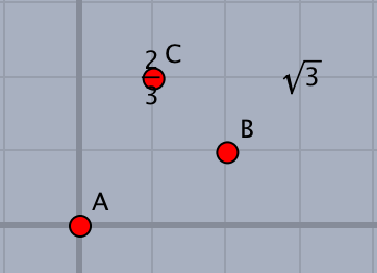
\includegraphics[bb=0.00 0.00 181.01 131.01,width=4cm]{Fig/exprrot.pdf} \hspace{10mm} %%% /Users/Hannya/Desktop/KeTCindy/fig/exprrot.tex 
%%% Generator=template1basic.cdy 
{\unitlength=8mm%
\begin{picture}%
(4.85,3.54)(-0.85,-0.54)%
\special{pn 8}%
%
{%
\color[rgb]{0,0,0}%
\settowidth{\Width}{\rotatebox[origin=c]{207}{$\frac{2}{3}$}}\setlength{\Width}{-0.5\Width}%
\settoheight{\Height}{\rotatebox[origin=c]{207}{$\frac{2}{3}$}}\settodepth{\Depth}{\rotatebox[origin=c]{207}{$\frac{2}{3}$}}\setlength{\Height}{-0.5\Height}\setlength{\Depth}{0.5\Depth}\addtolength{\Height}{\Depth}%
\put(1.0000000,2.0000000){\hspace*{\Width}\raisebox{\Height}{\rotatebox[origin=c]{207}{$\frac{2}{3}$}}}%
%
}%
{%
\color[rgb]{0,0,0}%
\settowidth{\Width}{\rotatebox[units=-360,origin=c]{27}{$\sqrt{3}$}}\setlength{\Width}{-0.5\Width}%
\settoheight{\Height}{\rotatebox[units=-360,origin=c]{27}{$\sqrt{3}$}}\settodepth{\Depth}{\rotatebox[units=-360,origin=c]{27}{$\sqrt{3}$}}\setlength{\Height}{-0.5\Height}\setlength{\Depth}{0.5\Depth}\addtolength{\Height}{\Depth}%
\put(3.0279508,2.0559017){\hspace*{\Width}\raisebox{\Height}{\rotatebox[units=-360,origin=c]{27}{$\sqrt{3}$}}}%
%
}%
\special{pa  -268    -0}\special{pa  1260    -0}%
\special{fp}%
\special{pa     0   170}\special{pa     0  -945}%
\special{fp}%
\settowidth{\Width}{$x$}\setlength{\Width}{0\Width}%
\settoheight{\Height}{$x$}\settodepth{\Depth}{$x$}\setlength{\Height}{-0.5\Height}\setlength{\Depth}{0.5\Depth}\addtolength{\Height}{\Depth}%
\put(4.0625000,0.0000000){\hspace*{\Width}\raisebox{\Height}{$x$}}%
%
\settowidth{\Width}{$y$}\setlength{\Width}{-0.5\Width}%
\settoheight{\Height}{$y$}\settodepth{\Depth}{$y$}\setlength{\Height}{\Depth}%
\put(0.0000000,3.0625000){\hspace*{\Width}\raisebox{\Height}{$y$}}%
%
\settowidth{\Width}{O}\setlength{\Width}{-1\Width}%
\settoheight{\Height}{O}\settodepth{\Depth}{O}\setlength{\Height}{-\Height}%
\put(-0.0625000,-0.0625000){\hspace*{\Width}\raisebox{\Height}{O}}%
%
\end{picture}}%

\vspace{\baselineskip}
\hypertarget{letter}{}\item[関数]  Letter([位置, 方向, 文字列])
\item[機能]  文字列を表示する
\item[説明]  「位置(座標)」と方向で指定された場所に文字を書き込む。

位置(座標)は点の名前で指定することもできる。

場所は上下左右を東西南北で表し, n/s/w/e/c   の方向で表す。cは中央。

%              \begin{center} %%% letter4.tex 2014-11-20 9:17
%%% sampleu3.sce 2014-11-17 19:14
{\unitlength=1cm%
\begin{picture}%
(   9.97000,   4.53000)(  -5.83000,  -2.11000)%
\special{pn 8}%
%
\normalsize%
\settowidth{\Width}{w}\setlength{\Width}{-0.5\Width}%
\settoheight{\Height}{w}\settodepth{\Depth}{w}\setlength{\Height}{-0.5\Height}\setlength{\Depth}{0.5\Depth}\addtolength{\Height}{\Depth}%
\put(-3.0000,0.0000){\hspace*{\Width}\raisebox{\Height}{w}}%
%
%
\settowidth{\Width}{e}\setlength{\Width}{-0.5\Width}%
\settoheight{\Height}{e}\settodepth{\Depth}{e}\setlength{\Height}{-0.5\Height}\setlength{\Depth}{0.5\Depth}\addtolength{\Height}{\Depth}%
\put(-1.0000,0.0000){\hspace*{\Width}\raisebox{\Height}{e}}%
%
%
\settowidth{\Width}{s}\setlength{\Width}{-0.5\Width}%
\settoheight{\Height}{s}\settodepth{\Depth}{s}\setlength{\Height}{-0.5\Height}\setlength{\Depth}{0.5\Depth}\addtolength{\Height}{\Depth}%
\put(-2.0000,-1.0000){\hspace*{\Width}\raisebox{\Height}{s}}%
%
%
\settowidth{\Width}{n}\setlength{\Width}{-0.5\Width}%
\settoheight{\Height}{n}\settodepth{\Depth}{n}\setlength{\Height}{-0.5\Height}\setlength{\Depth}{0.5\Depth}\addtolength{\Height}{\Depth}%
\put(-2.0000,1.0000){\hspace*{\Width}\raisebox{\Height}{n}}%
%
%
\settowidth{\Width}{w2}\setlength{\Width}{-0.5\Width}%
\settoheight{\Height}{w2}\settodepth{\Depth}{w2}\setlength{\Height}{-0.5\Height}\setlength{\Depth}{0.5\Depth}\addtolength{\Height}{\Depth}%
\put(-4.0000,0.0100){\hspace*{\Width}\raisebox{\Height}{w2}}%
%
%
\settowidth{\Width}{e2}\setlength{\Width}{-0.5\Width}%
\settoheight{\Height}{e2}\settodepth{\Depth}{e2}\setlength{\Height}{-0.5\Height}\setlength{\Depth}{0.5\Depth}\addtolength{\Height}{\Depth}%
\put(-0.0300,0.0100){\hspace*{\Width}\raisebox{\Height}{e2}}%
%
%
\settowidth{\Width}{c}\setlength{\Width}{-0.5\Width}%
\settoheight{\Height}{c}\settodepth{\Depth}{c}\setlength{\Height}{-0.5\Height}\setlength{\Depth}{0.5\Depth}\addtolength{\Height}{\Depth}%
\put(-2.0000,0.0000){\hspace*{\Width}\raisebox{\Height}{c}}%
%
%
\settowidth{\Width}{nw}\setlength{\Width}{-0.5\Width}%
\settoheight{\Height}{nw}\settodepth{\Depth}{nw}\setlength{\Height}{-0.5\Height}\setlength{\Depth}{0.5\Depth}\addtolength{\Height}{\Depth}%
\put(-2.7800,0.7300){\hspace*{\Width}\raisebox{\Height}{nw}}%
%
%
\settowidth{\Width}{sw}\setlength{\Width}{-0.5\Width}%
\settoheight{\Height}{sw}\settodepth{\Depth}{sw}\setlength{\Height}{-0.5\Height}\setlength{\Depth}{0.5\Depth}\addtolength{\Height}{\Depth}%
\put(-2.8100,-0.8100){\hspace*{\Width}\raisebox{\Height}{sw}}%
%
%
\settowidth{\Width}{ne}\setlength{\Width}{-0.5\Width}%
\settoheight{\Height}{ne}\settodepth{\Depth}{ne}\setlength{\Height}{-0.5\Height}\setlength{\Depth}{0.5\Depth}\addtolength{\Height}{\Depth}%
\put(-1.1600,0.8200){\hspace*{\Width}\raisebox{\Height}{ne}}%
%
%
\settowidth{\Width}{n2w2}\setlength{\Width}{-0.5\Width}%
\settoheight{\Height}{n2w2}\settodepth{\Depth}{n2w2}\setlength{\Height}{-0.5\Height}\setlength{\Depth}{0.5\Depth}\addtolength{\Height}{\Depth}%
\put(-3.6300,1.3800){\hspace*{\Width}\raisebox{\Height}{n2w2}}%
%
%
\settowidth{\Width}{e4}\setlength{\Width}{-0.5\Width}%
\settoheight{\Height}{e4}\settodepth{\Depth}{e4}\setlength{\Height}{-0.5\Height}\setlength{\Depth}{0.5\Depth}\addtolength{\Height}{\Depth}%
\put(1.9100,-0.0100){\hspace*{\Width}\raisebox{\Height}{e4}}%
%
%
\settowidth{\Width}{se}\setlength{\Width}{-0.5\Width}%
\settoheight{\Height}{se}\settodepth{\Depth}{se}\setlength{\Height}{-0.5\Height}\setlength{\Depth}{0.5\Depth}\addtolength{\Height}{\Depth}%
\put(-1.1700,-0.7800){\hspace*{\Width}\raisebox{\Height}{se}}%
%
%
\settowidth{\Width}{w3}\setlength{\Width}{-0.5\Width}%
\settoheight{\Height}{w3}\settodepth{\Depth}{w3}\setlength{\Height}{-0.5\Height}\setlength{\Depth}{0.5\Depth}\addtolength{\Height}{\Depth}%
\put(-4.6000,0.0100){\hspace*{\Width}\raisebox{\Height}{w3}}%
%
%
\settowidth{\Width}{w4}\setlength{\Width}{-0.5\Width}%
\settoheight{\Height}{w4}\settodepth{\Depth}{w4}\setlength{\Height}{-0.5\Height}\setlength{\Depth}{0.5\Depth}\addtolength{\Height}{\Depth}%
\put(-5.4000,0.0200){\hspace*{\Width}\raisebox{\Height}{w4}}%
%
%
\settowidth{\Width}{s2}\setlength{\Width}{-0.5\Width}%
\settoheight{\Height}{s2}\settodepth{\Depth}{s2}\setlength{\Height}{-0.5\Height}\setlength{\Depth}{0.5\Depth}\addtolength{\Height}{\Depth}%
\put(-1.9900,-1.2700){\hspace*{\Width}\raisebox{\Height}{s2}}%
%
%
\settowidth{\Width}{s3}\setlength{\Width}{-0.5\Width}%
\settoheight{\Height}{s3}\settodepth{\Depth}{s3}\setlength{\Height}{-0.5\Height}\setlength{\Depth}{0.5\Depth}\addtolength{\Height}{\Depth}%
\put(-1.9900,-1.5700){\hspace*{\Width}\raisebox{\Height}{s3}}%
%
%
\settowidth{\Width}{n2}\setlength{\Width}{-0.5\Width}%
\settoheight{\Height}{n2}\settodepth{\Depth}{n2}\setlength{\Height}{-0.5\Height}\setlength{\Depth}{0.5\Depth}\addtolength{\Height}{\Depth}%
\put(-2.0000,1.3800){\hspace*{\Width}\raisebox{\Height}{n2}}%
%
%
\settowidth{\Width}{n3}\setlength{\Width}{-0.5\Width}%
\settoheight{\Height}{n3}\settodepth{\Depth}{n3}\setlength{\Height}{-0.5\Height}\setlength{\Depth}{0.5\Depth}\addtolength{\Height}{\Depth}%
\put(-2.0000,1.7600){\hspace*{\Width}\raisebox{\Height}{n3}}%
%
%
\settowidth{\Width}{s4}\setlength{\Width}{-0.5\Width}%
\settoheight{\Height}{s4}\settodepth{\Depth}{s4}\setlength{\Height}{-0.5\Height}\setlength{\Depth}{0.5\Depth}\addtolength{\Height}{\Depth}%
\put(-1.9800,-1.9200){\hspace*{\Width}\raisebox{\Height}{s4}}%
%
%
\settowidth{\Width}{n4}\setlength{\Width}{-0.5\Width}%
\settoheight{\Height}{n4}\settodepth{\Depth}{n4}\setlength{\Height}{-0.5\Height}\setlength{\Depth}{0.5\Depth}\addtolength{\Height}{\Depth}%
\put(-1.9800,2.0900){\hspace*{\Width}\raisebox{\Height}{n4}}%
%
%
\settowidth{\Width}{s2w2}\setlength{\Width}{-0.5\Width}%
\settoheight{\Height}{s2w2}\settodepth{\Depth}{s2w2}\setlength{\Height}{-0.5\Height}\setlength{\Depth}{0.5\Depth}\addtolength{\Height}{\Depth}%
\put(-3.6300,-1.4400){\hspace*{\Width}\raisebox{\Height}{s2w2}}%
%
%
\settowidth{\Width}{s2e2}\setlength{\Width}{-0.5\Width}%
\settoheight{\Height}{s2e2}\settodepth{\Depth}{s2e2}\setlength{\Height}{-0.5\Height}\setlength{\Depth}{0.5\Depth}\addtolength{\Height}{\Depth}%
\put(-0.2900,-1.4300){\hspace*{\Width}\raisebox{\Height}{s2e2}}%
%
%
\settowidth{\Width}{n2e2}\setlength{\Width}{-0.5\Width}%
\settoheight{\Height}{n2e2}\settodepth{\Depth}{n2e2}\setlength{\Height}{-0.5\Height}\setlength{\Depth}{0.5\Depth}\addtolength{\Height}{\Depth}%
\put(-0.2400,1.4500){\hspace*{\Width}\raisebox{\Height}{n2e2}}%
%
%
\settowidth{\Width}{ne2}\setlength{\Width}{-0.5\Width}%
\settoheight{\Height}{ne2}\settodepth{\Depth}{ne2}\setlength{\Height}{-0.5\Height}\setlength{\Depth}{0.5\Depth}\addtolength{\Height}{\Depth}%
\put(-0.2700,0.7400){\hspace*{\Width}\raisebox{\Height}{ne2}}%
%
%
\settowidth{\Width}{e3}\setlength{\Width}{-0.5\Width}%
\settoheight{\Height}{e3}\settodepth{\Depth}{e3}\setlength{\Height}{-0.5\Height}\setlength{\Depth}{0.5\Depth}\addtolength{\Height}{\Depth}%
\put(1.2300,0.0000){\hspace*{\Width}\raisebox{\Height}{e3}}%
%
%
\special{pn 8}%
\special{pa -925 4}\special{pa -1067 4}%
\special{fp}%
\special{pn 8}%
\special{pa -992 -20}\special{pa -1067 4}\special{pa -992 28}\special{pa -992 4}\special{pa -992 -20}%
\special{sh 1}\special{ip}%
\special{pn 8}%
\special{pa -992 -20}\special{pa -1067 4}\special{pa -992 28}\special{pa -992 4}\special{pa -992 -20}%
\special{fp}%
\special{pn 8}%
\special{pn 8}%
\special{pa -787 -130}\special{pa -787 -276}%
\special{fp}%
\special{pn 8}%
\special{pa -763 -201}\special{pa -787 -276}\special{pa -812 -201}\special{pa -787 -201}%
\special{pa -763 -201}\special{sh 1}\special{ip}%
\special{pn 8}%
\special{pa -763 -201}\special{pa -787 -276}\special{pa -812 -201}\special{pa -787 -201}%
\special{pa -763 -201}%
\special{fp}%
\special{pn 8}%
\special{pn 8}%
\special{pa -787 134}\special{pa -787 295}%
\special{fp}%
\special{pn 8}%
\special{pa -812 220}\special{pa -787 295}\special{pa -763 220}\special{pa -787 220}%
\special{pa -812 220}\special{sh 1}\special{ip}%
\special{pn 8}%
\special{pa -812 220}\special{pa -787 295}\special{pa -763 220}\special{pa -787 220}%
\special{pa -812 220}%
\special{fp}%
\special{pn 8}%
\special{pn 8}%
\special{pa -661 -12}\special{pa -520 -4}%
\special{fp}%
\special{pn 8}%
\special{pa -596 16}\special{pa -520 -4}\special{pa -593 -32}\special{pa -594 -8}%
\special{pa -596 16}\special{sh 1}\special{ip}%
\special{pn 8}%
\special{pa -596 16}\special{pa -520 -4}\special{pa -593 -32}\special{pa -594 -8}%
\special{pa -596 16}%
\special{fp}%
\special{pn 8}%
\special{pn 8}%
\special{pa -1311 -4}\special{pa -1437 -4}%
\special{fp}%
\special{pn 8}%
\special{pa -1362 -28}\special{pa -1437 -4}\special{pa -1362 20}\special{pa -1362 -4}%
\special{pa -1362 -28}\special{sh 1}\special{ip}%
\special{pn 8}%
\special{pa -1362 -28}\special{pa -1437 -4}\special{pa -1362 20}\special{pa -1362 -4}%
\special{pa -1362 -28}%
\special{fp}%
\special{pn 8}%
\special{pn 8}%
\special{pa -295 8}\special{pa -177 0}%
\special{fp}%
\special{pn 8}%
\special{pa -250 29}\special{pa -177 0}\special{pa -254 -19}\special{pa -252 5}\special{pa -250 29}%
\special{sh 1}\special{ip}%
\special{pn 8}%
\special{pa -250 29}\special{pa -177 0}\special{pa -254 -19}\special{pa -252 5}\special{pa -250 29}%
\special{fp}%
\special{pn 8}%
\special{pn 8}%
\special{pa 189 4}\special{pa 319 4}%
\special{fp}%
\special{pn 8}%
\special{pa 244 28}\special{pa 319 4}\special{pa 244 -20}\special{pa 244 4}\special{pa 244 28}%
\special{sh 1}\special{ip}%
\special{pn 8}%
\special{pa 244 28}\special{pa 319 4}\special{pa 244 -20}\special{pa 244 4}\special{pa 244 28}%
\special{fp}%
\special{pn 8}%
\special{pn 8}%
\special{pa -331 -402}\special{pa -213 -484}%
\special{fp}%
\special{pn 8}%
\special{pa -260 -421}\special{pa -213 -484}\special{pa -288 -461}\special{pa -274 -441}%
\special{pa -260 -421}\special{sh 1}\special{ip}%
\special{pn 8}%
\special{pa -260 -421}\special{pa -213 -484}\special{pa -288 -461}\special{pa -274 -441}%
\special{pa -260 -421}%
\special{fp}%
\special{pn 8}%
\special{pn 8}%
\special{pa -350 390}\special{pa -220 484}%
\special{fp}%
\special{pn 8}%
\special{pa -295 460}\special{pa -220 484}\special{pa -267 421}\special{pa -281 440}%
\special{pa -295 460}\special{sh 1}\special{ip}%
\special{pn 8}%
\special{pa -295 460}\special{pa -220 484}\special{pa -267 421}\special{pa -281 440}%
\special{pa -295 460}%
\special{fp}%
\special{pn 8}%
\special{pn 8}%
\special{pa -1181 390}\special{pa -1276 469}%
\special{fp}%
\special{pn 8}%
\special{pa -1234 402}\special{pa -1276 469}\special{pa -1202 439}\special{pa -1218 421}%
\special{pa -1234 402}\special{sh 1}\special{ip}%
\special{pn 8}%
\special{pa -1234 402}\special{pa -1276 469}\special{pa -1202 439}\special{pa -1218 421}%
\special{pa -1234 402}%
\special{fp}%
\special{pn 8}%
\special{pn 8}%
\special{pa -693 106}\special{pa -606 205}%
\special{fp}%
\special{pn 8}%
\special{pa -674 165}\special{pa -606 205}\special{pa -638 132}\special{pa -656 149}%
\special{pa -674 165}\special{sh 1}\special{ip}%
\special{pn 8}%
\special{pa -674 165}\special{pa -606 205}\special{pa -638 132}\special{pa -656 149}%
\special{pa -674 165}%
\special{fp}%
\special{pn 8}%
\special{pn 8}%
\special{pa -669 -106}\special{pa -594 -189}%
\special{fp}%
\special{pn 8}%
\special{pa -627 -117}\special{pa -594 -189}\special{pa -663 -150}\special{pa -645 -133}%
\special{pa -627 -117}\special{sh 1}\special{ip}%
\special{pn 8}%
\special{pa -627 -117}\special{pa -594 -189}\special{pa -663 -150}\special{pa -645 -133}%
\special{pa -627 -117}%
\special{fp}%
\special{pn 8}%
\special{pn 8}%
\special{pa -886 -87}\special{pa -1008 -205}%
\special{fp}%
\special{pn 8}%
\special{pa -937 -170}\special{pa -1008 -205}\special{pa -971 -135}\special{pa -954 -153}%
\special{pa -937 -170}\special{sh 1}\special{ip}%
\special{pn 8}%
\special{pa -937 -170}\special{pa -1008 -205}\special{pa -971 -135}\special{pa -954 -153}%
\special{pa -937 -170}%
\special{fp}%
\special{pn 8}%
\special{pn 8}%
\special{pa -917 122}\special{pa -992 220}%
\special{fp}%
\special{pn 8}%
\special{pa -966 146}\special{pa -992 220}\special{pa -927 176}\special{pa -947 161}%
\special{pa -966 146}\special{sh 1}\special{ip}%
\special{pn 8}%
\special{pa -966 146}\special{pa -992 220}\special{pa -927 176}\special{pa -947 161}%
\special{pa -966 146}%
\special{fp}%
\special{pn 8}%
\special{pn 8}%
\special{pa -1189 -370}\special{pa -1311 -457}%
\special{fp}%
\special{pn 8}%
\special{pa -1236 -433}\special{pa -1311 -457}\special{pa -1264 -394}\special{pa -1250 -413}%
\special{pa -1236 -433}\special{sh 1}\special{ip}%
\special{pn 8}%
\special{pa -1236 -433}\special{pa -1311 -457}\special{pa -1264 -394}\special{pa -1250 -413}%
\special{pa -1236 -433}%
\special{fp}%
\special{pn 8}%
\settowidth{\Width}{$\cdot$}\setlength{\Width}{-0.5\Width}%
\settoheight{\Height}{$\cdot$}\settodepth{\Depth}{$\cdot$}\setlength{\Height}{-0.5\Height}\setlength{\Depth}{0.5\Depth}\addtolength{\Height}{\Depth}%
\put(3.4200,-0.0100){\hspace*{\Width}\raisebox{\Height}{$\cdot$}}%
%
%
\settowidth{\Width}{$\cdot$}\setlength{\Width}{-1\Width}%
\settoheight{\Height}{$\cdot$}\settodepth{\Depth}{$\cdot$}\setlength{\Height}{-0.5\Height}\setlength{\Depth}{0.5\Depth}\addtolength{\Height}{\Depth}%
\put(3.3700,-0.0100){\hspace*{\Width}\raisebox{\Height}{$\cdot$}}%
%
%
\settowidth{\Width}{$\cdot$}\setlength{\Width}{0\Width}%
\settoheight{\Height}{$\cdot$}\settodepth{\Depth}{$\cdot$}\setlength{\Height}{-0.5\Height}\setlength{\Depth}{0.5\Depth}\addtolength{\Height}{\Depth}%
\put(3.4700,-0.0100){\hspace*{\Width}\raisebox{\Height}{$\cdot$}}%
%
%
\settowidth{\Width}{$\cdot$}\setlength{\Width}{-0.5\Width}%
\settoheight{\Height}{$\cdot$}\settodepth{\Depth}{$\cdot$}\setlength{\Height}{\Depth}%
\put(3.4200,0.0400){\hspace*{\Width}\raisebox{\Height}{$\cdot$}}%
%
%
\settowidth{\Width}{$\cdot$}\setlength{\Width}{-0.5\Width}%
\settoheight{\Height}{$\cdot$}\settodepth{\Depth}{$\cdot$}\setlength{\Height}{-\Height}%
\put(3.4200,-0.0600){\hspace*{\Width}\raisebox{\Height}{$\cdot$}}%
%
%
\settowidth{\Width}{$\cdot$}\setlength{\Width}{0\Width}%
\settoheight{\Height}{$\cdot$}\settodepth{\Depth}{$\cdot$}\setlength{\Height}{\Depth}%
\put(3.4700,0.0400){\hspace*{\Width}\raisebox{\Height}{$\cdot$}}%
%
%
\settowidth{\Width}{$\cdot$}\setlength{\Width}{-1\Width}%
\settoheight{\Height}{$\cdot$}\settodepth{\Depth}{$\cdot$}\setlength{\Height}{\Depth}%
\put(3.3700,0.0400){\hspace*{\Width}\raisebox{\Height}{$\cdot$}}%
%
%
\settowidth{\Width}{$\cdot$}\setlength{\Width}{0\Width}%
\settoheight{\Height}{$\cdot$}\settodepth{\Depth}{$\cdot$}\setlength{\Height}{-\Height}%
\put(3.4700,-0.0600){\hspace*{\Width}\raisebox{\Height}{$\cdot$}}%
%
%
\settowidth{\Width}{$\cdot$}\setlength{\Width}{-1\Width}%
\settoheight{\Height}{$\cdot$}\settodepth{\Depth}{$\cdot$}\setlength{\Height}{-\Height}%
\put(3.3700,-0.0600){\hspace*{\Width}\raisebox{\Height}{$\cdot$}}%
%
%
\settowidth{\Width}{$\cdot$}\setlength{\Width}{-1\Width}%
\settoheight{\Height}{$\cdot$}\settodepth{\Depth}{$\cdot$}\setlength{\Height}{-0.5\Height}\setlength{\Depth}{0.5\Depth}\addtolength{\Height}{\Depth}%
\put(3.2700,-0.0100){\hspace*{\Width}\raisebox{\Height}{$\cdot$}}%
%
%
\settowidth{\Width}{$\cdot$}\setlength{\Width}{0\Width}%
\settoheight{\Height}{$\cdot$}\settodepth{\Depth}{$\cdot$}\setlength{\Height}{-0.5\Height}\setlength{\Depth}{0.5\Depth}\addtolength{\Height}{\Depth}%
\put(3.5700,-0.0100){\hspace*{\Width}\raisebox{\Height}{$\cdot$}}%
%
%
\settowidth{\Width}{$\cdot$}\setlength{\Width}{-0.5\Width}%
\settoheight{\Height}{$\cdot$}\settodepth{\Depth}{$\cdot$}\setlength{\Height}{\Depth}%
\put(3.4200,0.1400){\hspace*{\Width}\raisebox{\Height}{$\cdot$}}%
%
%
\settowidth{\Width}{$\cdot$}\setlength{\Width}{-0.5\Width}%
\settoheight{\Height}{$\cdot$}\settodepth{\Depth}{$\cdot$}\setlength{\Height}{-\Height}%
\put(3.4200,-0.1600){\hspace*{\Width}\raisebox{\Height}{$\cdot$}}%
%
%
\settowidth{\Width}{$\cdot$}\setlength{\Width}{0\Width}%
\settoheight{\Height}{$\cdot$}\settodepth{\Depth}{$\cdot$}\setlength{\Height}{\Depth}%
\put(3.5700,0.0400){\hspace*{\Width}\raisebox{\Height}{$\cdot$}}%
%
%
\settowidth{\Width}{$\cdot$}\setlength{\Width}{-1\Width}%
\settoheight{\Height}{$\cdot$}\settodepth{\Depth}{$\cdot$}\setlength{\Height}{\Depth}%
\put(3.2700,0.0400){\hspace*{\Width}\raisebox{\Height}{$\cdot$}}%
%
%
\settowidth{\Width}{$\cdot$}\setlength{\Width}{-0.5\Width}%
\settoheight{\Height}{$\cdot$}\settodepth{\Depth}{$\cdot$}\setlength{\Height}{\Depth}%
\put(3.4200,0.1400){\hspace*{\Width}\raisebox{\Height}{$\cdot$}}%
%
%
\settowidth{\Width}{$\cdot$}\setlength{\Width}{0\Width}%
\settoheight{\Height}{$\cdot$}\settodepth{\Depth}{$\cdot$}\setlength{\Height}{-\Height}%
\put(3.5700,-0.0600){\hspace*{\Width}\raisebox{\Height}{$\cdot$}}%
%
%
\settowidth{\Width}{$\cdot$}\setlength{\Width}{-1\Width}%
\settoheight{\Height}{$\cdot$}\settodepth{\Depth}{$\cdot$}\setlength{\Height}{-\Height}%
\put(3.2700,-0.0600){\hspace*{\Width}\raisebox{\Height}{$\cdot$}}%
%
%
\settowidth{\Width}{$\cdot$}\setlength{\Width}{0\Width}%
\settoheight{\Height}{$\cdot$}\settodepth{\Depth}{$\cdot$}\setlength{\Height}{\Depth}%
\put(3.4700,0.1400){\hspace*{\Width}\raisebox{\Height}{$\cdot$}}%
%
%
\settowidth{\Width}{$\cdot$}\setlength{\Width}{-1\Width}%
\settoheight{\Height}{$\cdot$}\settodepth{\Depth}{$\cdot$}\setlength{\Height}{\Depth}%
\put(3.3700,0.1400){\hspace*{\Width}\raisebox{\Height}{$\cdot$}}%
%
%
\settowidth{\Width}{$\cdot$}\setlength{\Width}{-0.5\Width}%
\settoheight{\Height}{$\cdot$}\settodepth{\Depth}{$\cdot$}\setlength{\Height}{\Depth}%
\put(3.4200,0.2400){\hspace*{\Width}\raisebox{\Height}{$\cdot$}}%
%
%
\settowidth{\Width}{$\cdot$}\setlength{\Width}{-0.5\Width}%
\settoheight{\Height}{$\cdot$}\settodepth{\Depth}{$\cdot$}\setlength{\Height}{\Depth}%
\put(3.4200,0.3400){\hspace*{\Width}\raisebox{\Height}{$\cdot$}}%
%
%
\settowidth{\Width}{$\cdot$}\setlength{\Width}{0\Width}%
\settoheight{\Height}{$\cdot$}\settodepth{\Depth}{$\cdot$}\setlength{\Height}{-\Height}%
\put(3.4700,-0.1600){\hspace*{\Width}\raisebox{\Height}{$\cdot$}}%
%
%
\settowidth{\Width}{$\cdot$}\setlength{\Width}{-1\Width}%
\settoheight{\Height}{$\cdot$}\settodepth{\Depth}{$\cdot$}\setlength{\Height}{-\Height}%
\put(3.3700,-0.1600){\hspace*{\Width}\raisebox{\Height}{$\cdot$}}%
%
%
\settowidth{\Width}{$\cdot$}\setlength{\Width}{0\Width}%
\settoheight{\Height}{$\cdot$}\settodepth{\Depth}{$\cdot$}\setlength{\Height}{\Depth}%
\put(3.5700,0.1400){\hspace*{\Width}\raisebox{\Height}{$\cdot$}}%
%
%
\settowidth{\Width}{$\cdot$}\setlength{\Width}{-1\Width}%
\settoheight{\Height}{$\cdot$}\settodepth{\Depth}{$\cdot$}\setlength{\Height}{\Depth}%
\put(3.2700,0.1400){\hspace*{\Width}\raisebox{\Height}{$\cdot$}}%
%
%
\settowidth{\Width}{$\cdot$}\setlength{\Width}{0\Width}%
\settoheight{\Height}{$\cdot$}\settodepth{\Depth}{$\cdot$}\setlength{\Height}{-\Height}%
\put(3.5700,-0.1600){\hspace*{\Width}\raisebox{\Height}{$\cdot$}}%
%
%
\settowidth{\Width}{$\cdot$}\setlength{\Width}{-1\Width}%
\settoheight{\Height}{$\cdot$}\settodepth{\Depth}{$\cdot$}\setlength{\Height}{-\Height}%
\put(3.2700,-0.1600){\hspace*{\Width}\raisebox{\Height}{$\cdot$}}%
%
%
\settowidth{\Width}{$\cdot$}\setlength{\Width}{-1\Width}%
\settoheight{\Height}{$\cdot$}\settodepth{\Depth}{$\cdot$}\setlength{\Height}{-0.5\Height}\setlength{\Depth}{0.5\Depth}\addtolength{\Height}{\Depth}%
\put(3.2200,-0.0100){\hspace*{\Width}\raisebox{\Height}{$\cdot$}}%
%
%
\settowidth{\Width}{$\cdot$}\setlength{\Width}{0\Width}%
\settoheight{\Height}{$\cdot$}\settodepth{\Depth}{$\cdot$}\setlength{\Height}{-0.5\Height}\setlength{\Depth}{0.5\Depth}\addtolength{\Height}{\Depth}%
\put(3.6200,-0.0100){\hspace*{\Width}\raisebox{\Height}{$\cdot$}}%
%
%
\settowidth{\Width}{$\cdot$}\setlength{\Width}{-0.5\Width}%
\settoheight{\Height}{$\cdot$}\settodepth{\Depth}{$\cdot$}\setlength{\Height}{\Depth}%
\put(3.4200,0.1900){\hspace*{\Width}\raisebox{\Height}{$\cdot$}}%
%
%
\settowidth{\Width}{$\cdot$}\setlength{\Width}{-0.5\Width}%
\settoheight{\Height}{$\cdot$}\settodepth{\Depth}{$\cdot$}\setlength{\Height}{-\Height}%
\put(3.4200,-0.2100){\hspace*{\Width}\raisebox{\Height}{$\cdot$}}%
%
%
\settowidth{\Width}{$\cdot$}\setlength{\Width}{0\Width}%
\settoheight{\Height}{$\cdot$}\settodepth{\Depth}{$\cdot$}\setlength{\Height}{\Depth}%
\put(3.6200,0.0400){\hspace*{\Width}\raisebox{\Height}{$\cdot$}}%
%
%
\settowidth{\Width}{$\cdot$}\setlength{\Width}{-1\Width}%
\settoheight{\Height}{$\cdot$}\settodepth{\Depth}{$\cdot$}\setlength{\Height}{\Depth}%
\put(3.2200,0.0400){\hspace*{\Width}\raisebox{\Height}{$\cdot$}}%
%
%
\settowidth{\Width}{$\cdot$}\setlength{\Width}{-0.5\Width}%
\settoheight{\Height}{$\cdot$}\settodepth{\Depth}{$\cdot$}\setlength{\Height}{\Depth}%
\put(3.4200,0.1900){\hspace*{\Width}\raisebox{\Height}{$\cdot$}}%
%
%
\settowidth{\Width}{$\cdot$}\setlength{\Width}{0\Width}%
\settoheight{\Height}{$\cdot$}\settodepth{\Depth}{$\cdot$}\setlength{\Height}{-\Height}%
\put(3.6200,-0.0600){\hspace*{\Width}\raisebox{\Height}{$\cdot$}}%
%
%
\settowidth{\Width}{$\cdot$}\setlength{\Width}{-1\Width}%
\settoheight{\Height}{$\cdot$}\settodepth{\Depth}{$\cdot$}\setlength{\Height}{-\Height}%
\put(3.2200,-0.0600){\hspace*{\Width}\raisebox{\Height}{$\cdot$}}%
%
%
\settowidth{\Width}{$\cdot$}\setlength{\Width}{0\Width}%
\settoheight{\Height}{$\cdot$}\settodepth{\Depth}{$\cdot$}\setlength{\Height}{\Depth}%
\put(3.6200,0.1900){\hspace*{\Width}\raisebox{\Height}{$\cdot$}}%
%
%
\settowidth{\Width}{$\cdot$}\setlength{\Width}{-1\Width}%
\settoheight{\Height}{$\cdot$}\settodepth{\Depth}{$\cdot$}\setlength{\Height}{\Depth}%
\put(3.2200,0.1900){\hspace*{\Width}\raisebox{\Height}{$\cdot$}}%
%
%
\settowidth{\Width}{$\cdot$}\setlength{\Width}{-0.5\Width}%
\settoheight{\Height}{$\cdot$}\settodepth{\Depth}{$\cdot$}\setlength{\Height}{-\Height}%
\put(3.4200,-0.2600){\hspace*{\Width}\raisebox{\Height}{$\cdot$}}%
%
%
\settowidth{\Width}{$\cdot$}\setlength{\Width}{-0.5\Width}%
\settoheight{\Height}{$\cdot$}\settodepth{\Depth}{$\cdot$}\setlength{\Height}{-\Height}%
\put(3.4200,-0.3600){\hspace*{\Width}\raisebox{\Height}{$\cdot$}}%
%
%
\settowidth{\Width}{$\cdot$}\setlength{\Width}{0\Width}%
\settoheight{\Height}{$\cdot$}\settodepth{\Depth}{$\cdot$}\setlength{\Height}{-0.5\Height}\setlength{\Depth}{0.5\Depth}\addtolength{\Height}{\Depth}%
\put(3.6700,-0.0100){\hspace*{\Width}\raisebox{\Height}{$\cdot$}}%
%
%
\settowidth{\Width}{$\cdot$}\setlength{\Width}{0\Width}%
\settoheight{\Height}{$\cdot$}\settodepth{\Depth}{$\cdot$}\setlength{\Height}{-0.5\Height}\setlength{\Depth}{0.5\Depth}\addtolength{\Height}{\Depth}%
\put(3.7700,-0.0100){\hspace*{\Width}\raisebox{\Height}{$\cdot$}}%
%
%
\settowidth{\Width}{$\cdot$}\setlength{\Width}{-1\Width}%
\settoheight{\Height}{$\cdot$}\settodepth{\Depth}{$\cdot$}\setlength{\Height}{-0.5\Height}\setlength{\Depth}{0.5\Depth}\addtolength{\Height}{\Depth}%
\put(3.1700,-0.0100){\hspace*{\Width}\raisebox{\Height}{$\cdot$}}%
%
%
\settowidth{\Width}{$\cdot$}\setlength{\Width}{-1\Width}%
\settoheight{\Height}{$\cdot$}\settodepth{\Depth}{$\cdot$}\setlength{\Height}{-0.5\Height}\setlength{\Depth}{0.5\Depth}\addtolength{\Height}{\Depth}%
\put(3.0700,-0.0100){\hspace*{\Width}\raisebox{\Height}{$\cdot$}}%
%
%
\settowidth{\Width}{$\cdot$}\setlength{\Width}{0\Width}%
\settoheight{\Height}{$\cdot$}\settodepth{\Depth}{$\cdot$}\setlength{\Height}{-\Height}%
\put(3.6200,-0.2100){\hspace*{\Width}\raisebox{\Height}{$\cdot$}}%
%
%
\special{pa -508 0}\special{pa -510 -35}\special{pa -517 -70}\special{pa -527 -103}%
\special{pa -542 -135}\special{pa -561 -164}\special{pa -584 -191}\special{pa -609 -215}%
\special{pa -638 -236}\special{pa -668 -253}\special{pa -701 -266}\special{pa -735 -275}%
\special{pa -770 -279}\special{pa -805 -279}\special{pa -840 -275}\special{pa -874 -266}%
\special{pa -906 -253}\special{pa -937 -236}\special{pa -966 -215}\special{pa -991 -191}%
\special{pa -1014 -164}\special{pa -1032 -135}\special{pa -1047 -103}\special{pa -1058 -70}%
\special{pa -1065 -35}\special{pa -1067 0}\special{pa -1065 35}\special{pa -1058 70}%
\special{pa -1047 103}\special{pa -1032 135}\special{pa -1014 164}\special{pa -991 191}%
\special{pa -966 215}\special{pa -937 236}\special{pa -906 253}\special{pa -874 266}%
\special{pa -840 275}\special{pa -805 279}\special{pa -770 279}\special{pa -735 275}%
\special{pa -701 266}\special{pa -668 253}\special{pa -638 236}\special{pa -609 215}%
\special{pa -584 191}\special{pa -561 164}\special{pa -542 135}\special{pa -527 103}%
\special{pa -517 70}\special{pa -510 35}\special{pa -508 0}%
\special{fp}%
\end{picture}}%
指定位置からの距離を,数値で与えることもでき,e2, e3 は e より少し離して置く。

複数の文字列をリストの形にして渡すことができる。

  注)導関数の記号$'$は,数式モード(\$ ではさむ)で$'$(シングルクウォート)を用いる。

\vspace{\baselineskip}
【例】

座標 (2,1) の南東にPを表示

\hspace{10mm}  \verb|Letter([[2,1] ,"se","P"]);|
        
点Cを中央としてCを表示

\hspace{10mm}  \verb|Letter([C ,"c", "C"]);|

点Aの南西にA,Eの南に数式を表示

\hspace{10mm}  \verb|Letter([A,"sw","A",E,"s","$ f(x)=\frac{1}{4} x^2 $"]);| 

\vspace{\baselineskip}
\hypertarget{letterrot}{}\item[関数]  Letterrot(座標, 方向ベクトル,移動量, 文字列)
\item[機能]  文字列を回転して表示する
\item[説明]  座標で示された位置に,方向ベクトルで指定された向きに回転して文字を書き込む。

第3引数は微小移動量で,略すこともできる。

\begin{verbatim}
      Letterrot(C,B-A,"t2n5","AB");
\end{verbatim}

移動量を略して

\hspace{10mm}  \verb|Letterrot(C,B-A,"AB");|

とすることもできる。この場合は,微小な移動はされない。

\begin{flushright}  \hyperlink{functionlist}{$\Rightarrow$関数一覧}\end{flushright}

\newpage
\end{description}
% ====== マーキング ==============
\subsubsection{マーキング}
\begin{description}

\hypertarget{anglemark}{}
\item[関数]  Anglemark(name,点リスト , options)
\item[機能]  点リストで示された角に弧の形状の角の印をつける。
\item[説明]  Listplot() などと同様,点リストが点名の場合はnameは省略できる。

optionsは次の通り。

数値      角の印の大きさ。 初期設定は1

線種      "dr, n"  , "da,m,n" , "do,m,n"

"Expr=文字"  : 文字を入れる

"Expr=位置 , 文字"  : 位置を指定して文字を入れる。位置は頂点からの距離。

\vspace{\baselineskip}
【例】三角形の内角に印をいれ,文字を書き込む。
\begin{verbatim}
      Listplot([A,B,C,A]);
      Letter([A,"n1","A",B,"w1","B",C,"e1","C"]);
      Anglemark([B,A,C]);
      Anglemark([C,B,A],["Expr=\theta"]);
      Anglemark([A,C,B],[2,"dr,3","Expr=2,\alpha"]);
\end{verbatim}

\hspace{20mm}%%% anglemark.tex 2014-11-10 8:47
%%% anglemark.sce 2014-11-10 8:36
{\unitlength=1cm%
\begin{picture}%
(   6.00000,   5.00000)(  -3.00000,  -2.00000)%
\special{pn 8}%
%
\settowidth{\Width}{A}\setlength{\Width}{-0.5\Width}%
\settoheight{\Height}{A}\settodepth{\Depth}{A}\setlength{\Height}{\Depth}%
\put(-0.4600,2.1100){\hspace*{\Width}\raisebox{\Height}{A}}%
%
%
\settowidth{\Width}{B}\setlength{\Width}{-1\Width}%
\settoheight{\Height}{B}\settodepth{\Depth}{B}\setlength{\Height}{-0.5\Height}\setlength{\Depth}{0.5\Depth}\addtolength{\Height}{\Depth}%
\put(-2.1000,-1.0000){\hspace*{\Width}\raisebox{\Height}{B}}%
%
%
\settowidth{\Width}{C}\setlength{\Width}{0\Width}%
\settoheight{\Height}{C}\settodepth{\Depth}{C}\setlength{\Height}{-0.5\Height}\setlength{\Depth}{0.5\Depth}\addtolength{\Height}{\Depth}%
\put(2.1000,-1.0000){\hspace*{\Width}\raisebox{\Height}{C}}%
%
%
\settowidth{\Width}{$\theta$}\setlength{\Width}{-0.5\Width}%
\settoheight{\Height}{$\theta$}\settodepth{\Depth}{$\theta$}\setlength{\Height}{-0.5\Height}\setlength{\Depth}{0.5\Depth}\addtolength{\Height}{\Depth}%
\put(-1.3600,-0.6100){\hspace*{\Width}\raisebox{\Height}{$\theta$}}%
%
%
\settowidth{\Width}{$\alpha$}\setlength{\Width}{-0.5\Width}%
\settoheight{\Height}{$\alpha$}\settodepth{\Depth}{$\alpha$}\setlength{\Height}{-0.5\Height}\setlength{\Depth}{0.5\Depth}\addtolength{\Height}{\Depth}%
\put(0.1900,-0.1400){\hspace*{\Width}\raisebox{\Height}{$\alpha$}}%
%
%
\special{pn 24}%
\special{pa 538 89}\special{pa 536 90}\special{pa 500 124}\special{pa 469 162}\special{pa 442 204}%
\special{pa 421 249}\special{pa 406 296}\special{pa 397 344}\special{pa 394 394}%
\special{fp}%
\special{pn 8}%
\special{pa -181 -791}\special{pa -787 394}\special{pa 787 394}\special{pa -181 -791}%
\special{fp}%
\special{pa -271 -616}\special{pa -265 -613}\special{pa -242 -604}\special{pa -218 -598}%
\special{pa -193 -595}\special{pa -169 -595}\special{pa -144 -598}\special{pa -120 -604}%
\special{pa -97 -613}\special{pa -76 -625}\special{pa -57 -639}%
\special{fp}%
\special{pa -591 394}\special{pa -592 369}\special{pa -597 345}\special{pa -604 321}%
\special{pa -615 299}\special{pa -628 278}\special{pa -644 259}\special{pa -662 242}%
\special{pa -682 227}\special{pa -698 219}%
\special{fp}%
\end{picture}}%

※角の印には平行四辺形の形状のものもある。\hyperlink{paramark}{Paramark()}を参照のこと。

\vspace{\baselineskip}
\hypertarget{paramark}{}
\item[関数]  Paramark(name,点リスト , options)
\item[機能]  点リストで示された角に平行四辺形の形状の角の印をつける。
\item[説明]  Listplot() などと同様,点リストが点名の場合はnameは省略できる。

optionsは次の通り。

数値  角の印の大きさ。 初期設定は1

線種  "dr, n"  , "da,m,n" , "do,m,n"

"Expr=文字"  : 文字を入れる

"Expr=位置 , 文字"  : 位置を指定して文字を入れる。位置は頂点からの距離。

\vspace{\baselineskip}
\begin{layer}{150}{0}
\putnotese{85}{0}{ %%% paramark.tex 2014-11-10 12:14
%%% bowdata.sce 2014-11-10 12:13
{\unitlength=1cm%
\begin{picture}%
(   6.00000,   6.00000)(  -3.00000,  -3.00000)%
\special{pn 8}%
%
\settowidth{\Width}{A}\setlength{\Width}{-0.5\Width}%
\settoheight{\Height}{A}\settodepth{\Depth}{A}\setlength{\Height}{\Depth}%
\put(-2.0000,2.1000){\hspace*{\Width}\raisebox{\Height}{A}}%
%
%
\settowidth{\Width}{B}\setlength{\Width}{-1\Width}%
\settoheight{\Height}{B}\settodepth{\Depth}{B}\setlength{\Height}{-0.5\Height}\setlength{\Depth}{0.5\Depth}\addtolength{\Height}{\Depth}%
\put(-2.1000,-2.0000){\hspace*{\Width}\raisebox{\Height}{B}}%
%
%
\settowidth{\Width}{C}\setlength{\Width}{0\Width}%
\settoheight{\Height}{C}\settodepth{\Depth}{C}\setlength{\Height}{-0.5\Height}\setlength{\Depth}{0.5\Depth}\addtolength{\Height}{\Depth}%
\put(2.1000,-2.0000){\hspace*{\Width}\raisebox{\Height}{C}}%
%
%
\settowidth{\Width}{$B$}\setlength{\Width}{-0.5\Width}%
\settoheight{\Height}{$B$}\settodepth{\Depth}{$B$}\setlength{\Height}{-0.5\Height}\setlength{\Depth}{0.5\Depth}\addtolength{\Height}{\Depth}%
\put(-0.8000,-0.8000){\hspace*{\Width}\raisebox{\Height}{$B$}}%
%
%
\settowidth{\Width}{$C$}\setlength{\Width}{-0.5\Width}%
\settoheight{\Height}{$C$}\settodepth{\Depth}{$C$}\setlength{\Height}{-0.5\Height}\setlength{\Depth}{0.5\Depth}\addtolength{\Height}{\Depth}%
\put(0.2900,-1.2900){\hspace*{\Width}\raisebox{\Height}{$C$}}%
%
%
\special{pn 16}%
\special{pa 648 648}\special{pa 451 648}\special{pa 591 787}%
\special{fp}%
\special{pn 8}%
\special{pa -787 -787}\special{pa -787 787}\special{pa 787 787}\special{pa -787 -787}%
\special{fp}%
\special{pa -787 -591}\special{pa -648 -451}\special{pa -648 -648}%
\special{fp}%
\special{pa -394 787}\special{pa -394 394}\special{pa -787 394}%
\special{fp}%
\end{picture}}%}
\end{layer}


【例】三角形の内角に印をいれ,文字を書き込む。

\begin{verbatim}
   Listplot([A,B,C,A]);
   Paramark([A,B,C]);
   Paramark([C,A,B],[3,"Expr=\alpha"]);
   Paramark([B,C,A],["dr,2","Expr=2,\theta"]);
   
\end{verbatim}

※角の印には弧の形状のものもある。\hyperlink{anglemark}{Anglemark()} を参照のこと。\\

\vspace{\baselineskip}
\hypertarget{bowdata}{}
\item[関数]  Bowdata(name,点リスト , options)
\item[機能]  弓形を描く
\item[説明]  点リストで与えられた2点を結ぶ弓形を描く。Listplot() などと同様,点リストが点名の場合はnameは省略できる。

2点を反時計回りに回る方向に弓形を描く。

optionsは,[曲がり , 空白サイズ  , 文字, 線種]

曲がり  は弧の曲がり具合の指定。 初期設定は1

空白サイズ  は中央にあける空白の大きさ

文字は,"Expr=文字" 

また,"Expr=微小移動 , 文字"  で位置を指定して文字を入れる。

微小移動は t  n 

 t は線分方向の微小移動。移動量は数字をつける。正負が可。

 n は線分と垂直方向の微小移動

\vspace{\baselineskip}
 \begin{layer}{150}{0}
\putnotese{85}{5}{ %%% fig.tex 2016-5-1 19:10
%%% fig.sce 2016-5-1 19:10
{\unitlength=8mm%
\begin{picture}%
(   4.50000,   5.00000)(  -1.00000,  -1.00000)%
\special{pn 8}%
%
\special{pa 414 -922}\special{pa 0 0}\special{pa 787 0}\special{pa 414 -922}%
\special{fp}%
\settowidth{\Width}{A}\setlength{\Width}{-0.5\Width}%
\settoheight{\Height}{A}\settodepth{\Depth}{A}\setlength{\Height}{\Depth}%
\put(1.3150,3.0277){\hspace*{\Width}\raisebox{\Height}{A}}%
%
%
\settowidth{\Width}{B}\setlength{\Width}{-1\Width}%
\settoheight{\Height}{B}\settodepth{\Depth}{B}\setlength{\Height}{-0.5\Height}\setlength{\Depth}{0.5\Depth}\addtolength{\Height}{\Depth}%
\put(-0.1000,0.0000){\hspace*{\Width}\raisebox{\Height}{B}}%
%
%
\settowidth{\Width}{C}\setlength{\Width}{0\Width}%
\settoheight{\Height}{C}\settodepth{\Depth}{C}\setlength{\Height}{-0.5\Height}\setlength{\Depth}{0.5\Depth}\addtolength{\Height}{\Depth}%
\put(2.6000,0.0000){\hspace*{\Width}\raisebox{\Height}{C}}%
%
%
\special{pa 414 -922}\special{pa 399 -908}\special{pa 384 -893}\special{pa 370 -878}%
\special{pa 355 -863}\special{pa 341 -848}\special{pa 328 -833}\special{pa 314 -817}%
\special{pa 301 -801}\special{pa 288 -785}\special{pa 275 -769}\special{pa 262 -752}%
\special{pa 250 -736}\special{pa 238 -719}\special{pa 226 -702}\special{pa 214 -684}%
\special{pa 203 -667}\special{pa 192 -649}\special{pa 182 -631}\special{pa 171 -613}%
\special{pa 161 -595}\special{pa 151 -577}\special{pa 142 -559}\special{pa 132 -540}%
\special{pa 124 -521}\special{pa 115 -502}\special{pa 107 -483}\special{pa 98 -464}%
\special{pa 91 -445}\special{pa 83 -426}\special{pa 76 -406}\special{pa 69 -387}\special{pa 63 -367}%
\special{pa 57 -347}\special{pa 51 -327}\special{pa 45 -307}\special{pa 40 -287}\special{pa 35 -267}%
\special{pa 30 -247}\special{pa 26 -227}\special{pa 22 -206}\special{pa 18 -186}\special{pa 15 -165}%
\special{pa 12 -145}\special{pa 9 -124}\special{pa 7 -104}\special{pa 5 -83}\special{pa 3 -62}%
\special{pa 2 -41}\special{pa 1 -21}\special{pa 0 0}%
\special{fp}%
\settowidth{\Width}{$a$}\setlength{\Width}{-0.5\Width}%
\settoheight{\Height}{$a$}\settodepth{\Depth}{$a$}\setlength{\Height}{-\Height}%
\put(1.2500,-0.4500){\hspace*{\Width}\raisebox{\Height}{$a$}}%
%
%
\special{pa 0 0}\special{pa 15 6}\special{pa 30 12}\special{pa 45 18}\special{pa 60 23}%
\special{pa 76 28}\special{pa 91 33}\special{pa 107 38}\special{pa 122 42}\special{pa 138 46}%
\special{pa 153 50}\special{pa 169 54}\special{pa 185 57}\special{pa 201 60}\special{pa 217 63}%
\special{pa 233 66}\special{pa 249 68}\special{pa 265 71}\special{pa 281 72}\special{pa 297 74}%
\special{pa 313 76}\special{pa 329 77}\special{pa 345 78}\special{pa 361 78}\special{pa 378 79}%
\special{pa 394 79}\special{pa 410 79}\special{pa 426 78}\special{pa 442 78}\special{pa 458 77}%
\special{pa 474 76}\special{pa 491 74}\special{pa 507 72}\special{pa 523 71}\special{pa 539 68}%
\special{pa 555 66}\special{pa 571 63}\special{pa 587 60}\special{pa 602 57}\special{pa 618 54}%
\special{pa 634 50}\special{pa 650 46}\special{pa 665 42}\special{pa 681 38}\special{pa 696 33}%
\special{pa 712 28}\special{pa 727 23}\special{pa 742 18}\special{pa 757 12}\special{pa 772 6}%
\special{pa 787 0}%
\special{fp}%
\settowidth{\Width}{$10$}\setlength{\Width}{-0.5\Width}%
\settoheight{\Height}{$10$}\settodepth{\Depth}{$10$}\setlength{\Height}{-0.5\Height}\setlength{\Depth}{0.5\Depth}\addtolength{\Height}{\Depth}%
\put(2.4930,1.7009){\hspace*{\Width}\raisebox{\Height}{$10$}}%
%
%
\special{pa 787 0}\special{pa 790 -7}\special{pa 793 -13}\special{pa 795 -20}\special{pa 797 -27}\special{pa 799 -31}\special{fp}%
\special{pa 809 -62}\special{pa 810 -68}\special{pa 812 -75}\special{pa 814 -82}\special{pa 816 -89}\special{pa 817 -93}\special{fp}%
\special{pa 824 -125}\special{pa 825 -131}\special{pa 827 -138}\special{pa 828 -145}\special{pa 829 -152}\special{pa 830 -158}\special{fp}%
\special{pa 834 -190}\special{pa 835 -195}\special{pa 835 -202}\special{pa 836 -210}\special{pa 836 -217}\special{pa 837 -223}\special{fp}%
\special{pa 838 -255}\special{pa 838 -260}\special{pa 838 -267}\special{pa 838 -274}\special{pa 838 -282}\special{pa 838 -288}\special{fp}%
\special{pa 836 -321}\special{pa 835 -325}\special{pa 835 -332}\special{pa 834 -339}\special{pa 833 -346}\special{pa 832 -353}\special{fp}%
\special{pa 692 -700}\special{pa 688 -705}\special{pa 684 -711}\special{pa 679 -717}\special{pa 674 -722}\special{pa 672 -725}\special{fp}%
\special{pa 651 -750}\special{pa 646 -755}\special{pa 641 -760}\special{pa 636 -765}\special{pa 631 -770}\special{pa 628 -774}\special{fp}%
\special{pa 604 -796}\special{pa 600 -800}\special{pa 595 -805}\special{pa 589 -810}\special{pa 584 -815}\special{pa 580 -818}\special{fp}%
\special{pa 554 -838}\special{pa 550 -842}\special{pa 544 -846}\special{pa 539 -850}\special{pa 533 -854}\special{pa 528 -858}\special{fp}%
\special{pa 501 -876}\special{pa 497 -878}\special{pa 491 -882}\special{pa 484 -886}\special{pa 478 -889}\special{pa 472 -892}\special{fp}%
\special{pa 444 -908}\special{pa 440 -910}\special{pa 434 -913}\special{pa 427 -916}\special{pa 421 -919}\special{pa 414 -922}\special{fp}%
%
%
\end{picture}}%}
 \end{layer}

【例】  三角形ABCの各辺に弓形マークをつけ記号を入れる。
\begin{verbatim}
      Listplot([A,B,C,A]);
      Letter([A,"n1","A",B,"w1","B",C,"e1","C"]);
      Bowdata([A,B]);
      Bowdata([B,C],[1,"Expr=t0n3,a"]);
      Bowdata([C,A],[2,1.2,"Expr=10","da"]);
\end{verbatim}

\vspace{\baselineskip}
これに加え,文字を回転して表示する方法がある。ただし,Cinderellaの画面には反映されない。文字をを回転するには次のように書く。

\hspace{10mm}"Exprrot=微小移動 , 文字"

 微小移動の最後にr をつけると,上下反転する。
 
以下にいくつか例を示す。
\begin{verbatim}
    Bowdata([B,A],[1,1,"Exprrot=a"]);
    Bowdata([D,C],[1,1,"Exprrot=t3n0,a"]);
    Bowdata([F,E],[1,1,"Exprrot=t-3n0,a"]);
    Bowdata([H,G],[1,1,"Exprrot=t0n3,a"]);
    Bowdata([L,K],[1,1,"Exprrot=t0n0r,a"]);
    Bowdata([N,M],[1,1,"Exprrot=t3n0r,a"]);
\end{verbatim}
\hspace{10mm} %%% test.tex 2014-11-30 22:4
%%% test.sce 2014-11-30 22:4
{\unitlength=6mm%
\begin{picture}%
(  20.00000,   7.00000)(  -3.00000,  -1.00000)%
\special{pn 8}%
%
\settowidth{\Width}{\rotatebox[origin=c]{59}{$a$}}\setlength{\Width}{-0.5\Width}%
\settoheight{\Height}{\rotatebox[origin=c]{59}{$a$}}\settodepth{\Depth}{\rotatebox[origin=c]{59}{$a$}}\setlength{\Height}{-0.5\Height}\setlength{\Depth}{0.5\Depth}\addtolength{\Height}{\Depth}%
\put(-1.0000,2.8000){\hspace*{\Width}\raisebox{\Height}{\rotatebox[origin=c]{59}{$a$}}}%
%
%
\settowidth{\Width}{\rotatebox[origin=c]{59}{$a$}}\setlength{\Width}{-0.5\Width}%
\settoheight{\Height}{\rotatebox[origin=c]{59}{$a$}}\settodepth{\Depth}{\rotatebox[origin=c]{59}{$a$}}\setlength{\Height}{-0.5\Height}\setlength{\Depth}{0.5\Depth}\addtolength{\Height}{\Depth}%
\put(2.0772,2.9286){\hspace*{\Width}\raisebox{\Height}{\rotatebox[origin=c]{59}{$a$}}}%
%
%
\settowidth{\Width}{\rotatebox[origin=c]{59}{$a$}}\setlength{\Width}{-0.5\Width}%
\settoheight{\Height}{\rotatebox[origin=c]{59}{$a$}}\settodepth{\Depth}{\rotatebox[origin=c]{59}{$a$}}\setlength{\Height}{-0.5\Height}\setlength{\Depth}{0.5\Depth}\addtolength{\Height}{\Depth}%
\put(4.9228,2.6714){\hspace*{\Width}\raisebox{\Height}{\rotatebox[origin=c]{59}{$a$}}}%
%
%
\settowidth{\Width}{\rotatebox[origin=c]{59}{$a$}}\setlength{\Width}{-0.5\Width}%
\settoheight{\Height}{\rotatebox[origin=c]{59}{$a$}}\settodepth{\Depth}{\rotatebox[origin=c]{59}{$a$}}\setlength{\Height}{-0.5\Height}\setlength{\Depth}{0.5\Depth}\addtolength{\Height}{\Depth}%
\put(7.8714,2.8772){\hspace*{\Width}\raisebox{\Height}{\rotatebox[origin=c]{59}{$a$}}}%
%
%
\settowidth{\Width}{\rotatebox[units=-360,origin=c]{121}{$a$}}\setlength{\Width}{-0.5\Width}%
\settoheight{\Height}{\rotatebox[units=-360,origin=c]{121}{$a$}}\settodepth{\Depth}{\rotatebox[units=-360,origin=c]{121}{$a$}}\setlength{\Height}{-0.5\Height}\setlength{\Depth}{0.5\Depth}\addtolength{\Height}{\Depth}%
\put(11.0000,2.8000){\hspace*{\Width}\raisebox{\Height}{\rotatebox[units=-360,origin=c]{121}{$a$}}}%
%
%
\settowidth{\Width}{\rotatebox[units=-360,origin=c]{121}{$a$}}\setlength{\Width}{-0.5\Width}%
\settoheight{\Height}{\rotatebox[units=-360,origin=c]{121}{$a$}}\settodepth{\Depth}{\rotatebox[units=-360,origin=c]{121}{$a$}}\setlength{\Height}{-0.5\Height}\setlength{\Depth}{0.5\Depth}\addtolength{\Height}{\Depth}%
\put(13.9228,2.6714){\hspace*{\Width}\raisebox{\Height}{\rotatebox[units=-360,origin=c]{121}{$a$}}}%
%
%
\settowidth{\Width}{rot}\setlength{\Width}{-0.5\Width}%
\settoheight{\Height}{rot}\settodepth{\Depth}{rot}\setlength{\Height}{-\Height}%
\put(-2.0000,-0.1500){\hspace*{\Width}\raisebox{\Height}{rot}}%
%
%
\settowidth{\Width}{t3}\setlength{\Width}{-0.5\Width}%
\settoheight{\Height}{t3}\settodepth{\Depth}{t3}\setlength{\Height}{-\Height}%
\put(1.0000,-0.1500){\hspace*{\Width}\raisebox{\Height}{t3}}%
%
%
\settowidth{\Width}{t-3}\setlength{\Width}{-0.5\Width}%
\settoheight{\Height}{t-3}\settodepth{\Depth}{t-3}\setlength{\Height}{-\Height}%
\put(4.0000,-0.1500){\hspace*{\Width}\raisebox{\Height}{t-3}}%
%
%
\settowidth{\Width}{n3}\setlength{\Width}{-0.5\Width}%
\settoheight{\Height}{n3}\settodepth{\Depth}{n3}\setlength{\Height}{-\Height}%
\put(7.0000,-0.1500){\hspace*{\Width}\raisebox{\Height}{n3}}%
%
%
\settowidth{\Width}{u}\setlength{\Width}{-0.5\Width}%
\settoheight{\Height}{u}\settodepth{\Depth}{u}\setlength{\Height}{-\Height}%
\put(10.0000,-0.1500){\hspace*{\Width}\raisebox{\Height}{u}}%
%
%
\settowidth{\Width}{t3u}\setlength{\Width}{-0.5\Width}%
\settoheight{\Height}{t3u}\settodepth{\Depth}{t3u}\setlength{\Height}{-\Height}%
\put(13.0000,-0.1500){\hspace*{\Width}\raisebox{\Height}{t3u}}%
%
%
\special{pa -472 0}\special{pa 236 -1181}%
\special{fp}%
\special{pa 236 0}\special{pa 945 -1181}%
\special{fp}%
\special{pa 945 0}\special{pa 1654 -1181}%
\special{fp}%
\special{pa 1654 0}\special{pa 2362 -1181}%
\special{fp}%
\special{pa 2362 0}\special{pa 3071 -1181}%
\special{fp}%
\special{pa 3071 0}\special{pa 3780 -1181}%
\special{fp}%
\special{pa 236 -1181}\special{pa 227 -1174}\special{pa 217 -1167}\special{pa 208 -1160}%
\special{pa 199 -1153}\special{pa 189 -1145}\special{pa 180 -1138}\special{pa 171 -1131}%
\special{pa 162 -1123}\special{pa 153 -1116}\special{pa 144 -1108}\special{pa 135 -1101}%
\special{pa 126 -1093}\special{pa 117 -1085}\special{pa 108 -1077}\special{pa 99 -1069}%
\special{pa 91 -1061}\special{pa 82 -1054}\special{pa 73 -1045}\special{pa 65 -1037}%
\special{pa 56 -1029}\special{pa 48 -1021}\special{pa 40 -1013}\special{pa 31 -1004}%
\special{pa 23 -996}\special{pa 15 -988}\special{pa 7 -979}\special{pa -2 -971}\special{pa -10 -962}%
\special{pa -18 -953}\special{pa -26 -945}\special{pa -34 -936}\special{pa -41 -927}%
\special{pa -49 -918}\special{pa -57 -910}\special{pa -65 -901}\special{pa -72 -892}%
\special{pa -80 -883}\special{pa -87 -873}\special{pa -95 -864}\special{pa -102 -855}%
\special{pa -109 -846}\special{pa -116 -837}\special{pa -124 -827}\special{pa -131 -818}%
\special{pa -138 -808}\special{pa -145 -799}\special{pa -152 -789}\special{pa -159 -780}%
\special{pa -165 -770}\special{pa -172 -761}%
\special{fp}%
\special{pa -294 -558}\special{pa -299 -548}\special{pa -304 -537}\special{pa -309 -527}%
\special{pa -315 -516}\special{pa -320 -505}\special{pa -325 -495}\special{pa -330 -484}%
\special{pa -334 -473}\special{pa -339 -463}\special{pa -344 -452}\special{pa -349 -441}%
\special{pa -353 -430}\special{pa -358 -419}\special{pa -362 -408}\special{pa -366 -397}%
\special{pa -371 -386}\special{pa -375 -375}\special{pa -379 -364}\special{pa -383 -353}%
\special{pa -387 -342}\special{pa -391 -331}\special{pa -395 -320}\special{pa -399 -309}%
\special{pa -402 -298}\special{pa -406 -286}\special{pa -410 -275}\special{pa -413 -264}%
\special{pa -416 -253}\special{pa -420 -241}\special{pa -423 -230}\special{pa -426 -219}%
\special{pa -429 -207}\special{pa -432 -196}\special{pa -435 -185}\special{pa -438 -173}%
\special{pa -441 -162}\special{pa -444 -150}\special{pa -446 -139}\special{pa -449 -127}%
\special{pa -452 -116}\special{pa -454 -104}\special{pa -456 -93}\special{pa -459 -81}%
\special{pa -461 -70}\special{pa -463 -58}\special{pa -465 -47}\special{pa -467 -35}%
\special{pa -469 -23}\special{pa -471 -12}\special{pa -472 0}%
\special{fp}%
\special{pa 945 -1181}\special{pa 935 -1174}\special{pa 926 -1167}\special{pa 917 -1160}%
\special{pa 907 -1153}\special{pa 898 -1145}\special{pa 889 -1138}\special{pa 880 -1131}%
\special{pa 871 -1123}\special{pa 862 -1116}\special{pa 852 -1108}\special{pa 844 -1101}%
\special{pa 835 -1093}\special{pa 826 -1085}\special{pa 817 -1077}\special{pa 808 -1069}%
\special{pa 799 -1061}\special{pa 791 -1054}\special{pa 782 -1045}\special{pa 774 -1037}%
\special{pa 765 -1029}\special{pa 757 -1021}\special{pa 748 -1013}\special{pa 740 -1004}%
\special{pa 732 -996}\special{pa 723 -988}\special{pa 715 -979}\special{pa 707 -971}%
\special{pa 699 -962}\special{pa 691 -953}\special{pa 683 -945}\special{pa 675 -936}%
\special{pa 667 -927}\special{pa 660 -918}\special{pa 652 -910}\special{pa 644 -901}%
\special{pa 637 -892}\special{pa 629 -883}\special{pa 622 -873}\special{pa 614 -864}%
\special{pa 607 -855}\special{pa 599 -846}\special{pa 592 -837}\special{pa 585 -827}%
\special{pa 578 -818}\special{pa 571 -808}\special{pa 564 -799}\special{pa 557 -789}%
\special{pa 550 -780}\special{pa 543 -770}\special{pa 537 -761}%
\special{fp}%
\special{pa 415 -558}\special{pa 410 -548}\special{pa 404 -537}\special{pa 399 -527}%
\special{pa 394 -516}\special{pa 389 -505}\special{pa 384 -495}\special{pa 379 -484}%
\special{pa 374 -473}\special{pa 369 -463}\special{pa 365 -452}\special{pa 360 -441}%
\special{pa 356 -430}\special{pa 351 -419}\special{pa 347 -408}\special{pa 342 -397}%
\special{pa 338 -386}\special{pa 334 -375}\special{pa 330 -364}\special{pa 326 -353}%
\special{pa 322 -342}\special{pa 318 -331}\special{pa 314 -320}\special{pa 310 -309}%
\special{pa 306 -298}\special{pa 303 -286}\special{pa 299 -275}\special{pa 296 -264}%
\special{pa 292 -253}\special{pa 289 -241}\special{pa 286 -230}\special{pa 282 -219}%
\special{pa 279 -207}\special{pa 276 -196}\special{pa 273 -185}\special{pa 270 -173}%
\special{pa 268 -162}\special{pa 265 -150}\special{pa 262 -139}\special{pa 260 -127}%
\special{pa 257 -116}\special{pa 255 -104}\special{pa 252 -93}\special{pa 250 -81}%
\special{pa 248 -70}\special{pa 246 -58}\special{pa 244 -47}\special{pa 242 -35}\special{pa 240 -23}%
\special{pa 238 -12}\special{pa 236 0}%
\special{fp}%
\special{pa 1654 -1181}\special{pa 1644 -1174}\special{pa 1635 -1167}\special{pa 1625 -1160}%
\special{pa 1616 -1153}\special{pa 1607 -1145}\special{pa 1598 -1138}\special{pa 1588 -1131}%
\special{pa 1579 -1123}\special{pa 1570 -1116}\special{pa 1561 -1108}\special{pa 1552 -1101}%
\special{pa 1543 -1093}\special{pa 1534 -1085}\special{pa 1526 -1077}\special{pa 1517 -1069}%
\special{pa 1508 -1061}\special{pa 1499 -1054}\special{pa 1491 -1045}\special{pa 1482 -1037}%
\special{pa 1474 -1029}\special{pa 1465 -1021}\special{pa 1457 -1013}\special{pa 1449 -1004}%
\special{pa 1440 -996}\special{pa 1432 -988}\special{pa 1424 -979}\special{pa 1416 -971}%
\special{pa 1408 -962}\special{pa 1400 -953}\special{pa 1392 -945}\special{pa 1384 -936}%
\special{pa 1376 -927}\special{pa 1368 -918}\special{pa 1360 -910}\special{pa 1353 -901}%
\special{pa 1345 -892}\special{pa 1338 -883}\special{pa 1330 -873}\special{pa 1323 -864}%
\special{pa 1315 -855}\special{pa 1308 -846}\special{pa 1301 -837}\special{pa 1294 -827}%
\special{pa 1287 -818}\special{pa 1280 -808}\special{pa 1273 -799}\special{pa 1266 -789}%
\special{pa 1259 -780}\special{pa 1252 -770}\special{pa 1245 -761}%
\special{fp}%
\special{pa 1124 -558}\special{pa 1118 -548}\special{pa 1113 -537}\special{pa 1108 -527}%
\special{pa 1103 -516}\special{pa 1098 -505}\special{pa 1093 -495}\special{pa 1088 -484}%
\special{pa 1083 -473}\special{pa 1078 -463}\special{pa 1073 -452}\special{pa 1069 -441}%
\special{pa 1064 -430}\special{pa 1060 -419}\special{pa 1055 -408}\special{pa 1051 -397}%
\special{pa 1047 -386}\special{pa 1042 -375}\special{pa 1038 -364}\special{pa 1034 -353}%
\special{pa 1030 -342}\special{pa 1026 -331}\special{pa 1022 -320}\special{pa 1019 -309}%
\special{pa 1015 -298}\special{pa 1011 -286}\special{pa 1008 -275}\special{pa 1004 -264}%
\special{pa 1001 -253}\special{pa 998 -241}\special{pa 994 -230}\special{pa 991 -219}%
\special{pa 988 -207}\special{pa 985 -196}\special{pa 982 -185}\special{pa 979 -173}%
\special{pa 976 -162}\special{pa 974 -150}\special{pa 971 -139}\special{pa 968 -127}%
\special{pa 966 -116}\special{pa 963 -104}\special{pa 961 -93}\special{pa 959 -81}%
\special{pa 957 -70}\special{pa 954 -58}\special{pa 952 -47}\special{pa 950 -35}\special{pa 948 -23}%
\special{pa 947 -12}\special{pa 945 0}%
\special{fp}%
\special{pa 2362 -1181}\special{pa 2353 -1174}\special{pa 2343 -1167}\special{pa 2334 -1160}%
\special{pa 2325 -1153}\special{pa 2315 -1145}\special{pa 2306 -1138}\special{pa 2297 -1131}%
\special{pa 2288 -1123}\special{pa 2279 -1116}\special{pa 2270 -1108}\special{pa 2261 -1101}%
\special{pa 2252 -1093}\special{pa 2243 -1085}\special{pa 2234 -1077}\special{pa 2225 -1069}%
\special{pa 2217 -1061}\special{pa 2208 -1054}\special{pa 2199 -1045}\special{pa 2191 -1037}%
\special{pa 2182 -1029}\special{pa 2174 -1021}\special{pa 2166 -1013}\special{pa 2157 -1004}%
\special{pa 2149 -996}\special{pa 2141 -988}\special{pa 2133 -979}\special{pa 2124 -971}%
\special{pa 2116 -962}\special{pa 2108 -953}\special{pa 2100 -945}\special{pa 2092 -936}%
\special{pa 2085 -927}\special{pa 2077 -918}\special{pa 2069 -910}\special{pa 2061 -901}%
\special{pa 2054 -892}\special{pa 2046 -883}\special{pa 2039 -873}\special{pa 2031 -864}%
\special{pa 2024 -855}\special{pa 2017 -846}\special{pa 2010 -837}\special{pa 2002 -827}%
\special{pa 1995 -818}\special{pa 1988 -808}\special{pa 1981 -799}\special{pa 1974 -789}%
\special{pa 1967 -780}\special{pa 1961 -770}\special{pa 1954 -761}%
\special{fp}%
\special{pa 1832 -558}\special{pa 1827 -548}\special{pa 1822 -537}\special{pa 1817 -527}%
\special{pa 1811 -516}\special{pa 1806 -505}\special{pa 1801 -495}\special{pa 1796 -484}%
\special{pa 1792 -473}\special{pa 1787 -463}\special{pa 1782 -452}\special{pa 1777 -441}%
\special{pa 1773 -430}\special{pa 1768 -419}\special{pa 1764 -408}\special{pa 1760 -397}%
\special{pa 1755 -386}\special{pa 1751 -375}\special{pa 1747 -364}\special{pa 1743 -353}%
\special{pa 1739 -342}\special{pa 1735 -331}\special{pa 1731 -320}\special{pa 1727 -309}%
\special{pa 1724 -298}\special{pa 1720 -286}\special{pa 1716 -275}\special{pa 1713 -264}%
\special{pa 1710 -253}\special{pa 1706 -241}\special{pa 1703 -230}\special{pa 1700 -219}%
\special{pa 1697 -207}\special{pa 1694 -196}\special{pa 1691 -185}\special{pa 1688 -173}%
\special{pa 1685 -162}\special{pa 1682 -150}\special{pa 1680 -139}\special{pa 1677 -127}%
\special{pa 1674 -116}\special{pa 1672 -104}\special{pa 1670 -93}\special{pa 1667 -81}%
\special{pa 1665 -70}\special{pa 1663 -58}\special{pa 1661 -47}\special{pa 1659 -35}%
\special{pa 1657 -23}\special{pa 1655 -12}\special{pa 1654 0}%
\special{fp}%
\special{pa 3071 -1181}\special{pa 3061 -1174}\special{pa 3052 -1167}\special{pa 3043 -1160}%
\special{pa 3033 -1153}\special{pa 3024 -1145}\special{pa 3015 -1138}\special{pa 3006 -1131}%
\special{pa 2997 -1123}\special{pa 2987 -1116}\special{pa 2978 -1108}\special{pa 2969 -1101}%
\special{pa 2961 -1093}\special{pa 2952 -1085}\special{pa 2943 -1077}\special{pa 2934 -1069}%
\special{pa 2925 -1061}\special{pa 2917 -1054}\special{pa 2908 -1045}\special{pa 2900 -1037}%
\special{pa 2891 -1029}\special{pa 2883 -1021}\special{pa 2874 -1013}\special{pa 2866 -1004}%
\special{pa 2858 -996}\special{pa 2849 -988}\special{pa 2841 -979}\special{pa 2833 -971}%
\special{pa 2825 -962}\special{pa 2817 -953}\special{pa 2809 -945}\special{pa 2801 -936}%
\special{pa 2793 -927}\special{pa 2786 -918}\special{pa 2778 -910}\special{pa 2770 -901}%
\special{pa 2763 -892}\special{pa 2755 -883}\special{pa 2748 -873}\special{pa 2740 -864}%
\special{pa 2733 -855}\special{pa 2725 -846}\special{pa 2718 -837}\special{pa 2711 -827}%
\special{pa 2704 -818}\special{pa 2697 -808}\special{pa 2690 -799}\special{pa 2683 -789}%
\special{pa 2676 -780}\special{pa 2669 -770}\special{pa 2662 -761}%
\special{fp}%
\special{pa 2541 -558}\special{pa 2536 -548}\special{pa 2530 -537}\special{pa 2525 -527}%
\special{pa 2520 -516}\special{pa 2515 -505}\special{pa 2510 -495}\special{pa 2505 -484}%
\special{pa 2500 -473}\special{pa 2495 -463}\special{pa 2491 -452}\special{pa 2486 -441}%
\special{pa 2482 -430}\special{pa 2477 -419}\special{pa 2473 -408}\special{pa 2468 -397}%
\special{pa 2464 -386}\special{pa 2460 -375}\special{pa 2456 -364}\special{pa 2452 -353}%
\special{pa 2448 -342}\special{pa 2444 -331}\special{pa 2440 -320}\special{pa 2436 -309}%
\special{pa 2432 -298}\special{pa 2429 -286}\special{pa 2425 -275}\special{pa 2422 -264}%
\special{pa 2418 -253}\special{pa 2415 -241}\special{pa 2412 -230}\special{pa 2408 -219}%
\special{pa 2405 -207}\special{pa 2402 -196}\special{pa 2399 -185}\special{pa 2396 -173}%
\special{pa 2394 -162}\special{pa 2391 -150}\special{pa 2388 -139}\special{pa 2386 -127}%
\special{pa 2383 -116}\special{pa 2381 -104}\special{pa 2378 -93}\special{pa 2376 -81}%
\special{pa 2374 -70}\special{pa 2372 -58}\special{pa 2370 -47}\special{pa 2368 -35}%
\special{pa 2366 -23}\special{pa 2364 -12}\special{pa 2362 0}%
\special{fp}%
\special{pa 3780 -1181}\special{pa 3770 -1174}\special{pa 3761 -1167}\special{pa 3751 -1160}%
\special{pa 3742 -1153}\special{pa 3733 -1145}\special{pa 3724 -1138}\special{pa 3714 -1131}%
\special{pa 3705 -1123}\special{pa 3696 -1116}\special{pa 3687 -1108}\special{pa 3678 -1101}%
\special{pa 3669 -1093}\special{pa 3660 -1085}\special{pa 3652 -1077}\special{pa 3643 -1069}%
\special{pa 3634 -1061}\special{pa 3625 -1054}\special{pa 3617 -1045}\special{pa 3608 -1037}%
\special{pa 3600 -1029}\special{pa 3591 -1021}\special{pa 3583 -1013}\special{pa 3575 -1004}%
\special{pa 3566 -996}\special{pa 3558 -988}\special{pa 3550 -979}\special{pa 3542 -971}%
\special{pa 3534 -962}\special{pa 3526 -953}\special{pa 3518 -945}\special{pa 3510 -936}%
\special{pa 3502 -927}\special{pa 3494 -918}\special{pa 3486 -910}\special{pa 3479 -901}%
\special{pa 3471 -892}\special{pa 3464 -883}\special{pa 3456 -873}\special{pa 3449 -864}%
\special{pa 3441 -855}\special{pa 3434 -846}\special{pa 3427 -837}\special{pa 3420 -827}%
\special{pa 3413 -818}\special{pa 3405 -808}\special{pa 3398 -799}\special{pa 3392 -789}%
\special{pa 3385 -780}\special{pa 3378 -770}\special{pa 3371 -761}%
\special{fp}%
\special{pa 3250 -558}\special{pa 3244 -548}\special{pa 3239 -537}\special{pa 3234 -527}%
\special{pa 3229 -516}\special{pa 3224 -505}\special{pa 3219 -495}\special{pa 3214 -484}%
\special{pa 3209 -473}\special{pa 3204 -463}\special{pa 3199 -452}\special{pa 3195 -441}%
\special{pa 3190 -430}\special{pa 3186 -419}\special{pa 3181 -408}\special{pa 3177 -397}%
\special{pa 3173 -386}\special{pa 3168 -375}\special{pa 3164 -364}\special{pa 3160 -353}%
\special{pa 3156 -342}\special{pa 3152 -331}\special{pa 3148 -320}\special{pa 3145 -309}%
\special{pa 3141 -298}\special{pa 3137 -286}\special{pa 3134 -275}\special{pa 3130 -264}%
\special{pa 3127 -253}\special{pa 3124 -241}\special{pa 3120 -230}\special{pa 3117 -219}%
\special{pa 3114 -207}\special{pa 3111 -196}\special{pa 3108 -185}\special{pa 3105 -173}%
\special{pa 3102 -162}\special{pa 3100 -150}\special{pa 3097 -139}\special{pa 3094 -127}%
\special{pa 3092 -116}\special{pa 3089 -104}\special{pa 3087 -93}\special{pa 3085 -81}%
\special{pa 3082 -70}\special{pa 3080 -58}\special{pa 3078 -47}\special{pa 3076 -35}%
\special{pa 3074 -23}\special{pa 3073 -12}\special{pa 3071 0}%
\special{fp}%
\end{picture}}%

%\begin{flushright}  \hyperlink{functionlist}{$\Rightarrow$関数一覧}\end{flushright}

\hypertarget{drawsegmark}{}
\item[関数]  Drawsegmark(name,リスト,options)または Segmark(name,リスト,options)
\item[機能]  線分に印をつける
\item[説明]  リストで与えられた2点を端点とする線分に印をつける。印には4種類がある。

optionsは
\begin{tabbing}
1234\=56789012\=345678901234567890\=\kill
 \> Type=n \>:印の種類 n=1〜4\\
 \> Width  \>:二本線のときの線の幅
\end{tabbing}

  【例】四角形ABCDを描き線分に印をつける。
  
\begin{layer}{150}{0}
\putnotese{90}{5}{ %%% fig.tex 2015-8-8 7:41
%%% fig.sce 2015-8-8 7:37
{\unitlength=6mm%
\begin{picture}%
(   4.84000,   3.93000)(  -0.24000,  -0.41000)%
\special{pn 8}%
%
\special{pa 236 -709}\special{pa 0 0}\special{pa 945 0}\special{pa 800 -564}\special{pa 236 -709}%
\special{fp}%
\special{pa 151 -343}\special{pa 85 -366}%
\special{fp}%
\special{pa 491 -35}\special{pa 491 35}%
\special{fp}%
\special{pa 454 -35}\special{pa 454 35}%
\special{fp}%
\special{pa 908 -281}\special{pa 908 -286}\special{pa 907 -290}\special{pa 905 -294}%
\special{pa 903 -299}\special{pa 901 -302}\special{pa 898 -306}\special{pa 895 -309}%
\special{pa 891 -312}\special{pa 887 -314}\special{pa 883 -315}\special{pa 878 -317}%
\special{pa 874 -317}\special{pa 869 -317}\special{pa 865 -317}\special{pa 860 -315}%
\special{pa 856 -314}\special{pa 852 -312}\special{pa 849 -309}\special{pa 845 -306}%
\special{pa 842 -302}\special{pa 840 -299}\special{pa 838 -294}\special{pa 837 -290}%
\special{pa 836 -286}\special{pa 836 -281}\special{pa 836 -277}\special{pa 837 -272}%
\special{pa 838 -268}\special{pa 840 -264}\special{pa 842 -260}\special{pa 845 -256}%
\special{pa 849 -253}\special{pa 852 -251}\special{pa 856 -248}\special{pa 860 -247}%
\special{pa 865 -246}\special{pa 869 -245}\special{pa 874 -245}\special{pa 878 -246}%
\special{pa 883 -247}\special{pa 887 -248}\special{pa 891 -251}\special{pa 895 -253}%
\special{pa 898 -256}\special{pa 901 -260}\special{pa 903 -264}\special{pa 905 -268}%
\special{pa 907 -272}\special{pa 908 -277}\special{pa 908 -281}%
\special{fp}%
\special{pa 508 -598}\special{pa 489 -664}\special{pa 557 -647}\special{pa 508 -598}%
\special{fp}%
\settowidth{\Width}{A}\setlength{\Width}{-0.5\Width}%
\settoheight{\Height}{A}\settodepth{\Depth}{A}\setlength{\Height}{\Depth}%
\put(1.0000,3.0500){\hspace*{\Width}\raisebox{\Height}{A}}%
%
%
\settowidth{\Width}{B}\setlength{\Width}{-1\Width}%
\settoheight{\Height}{B}\settodepth{\Depth}{B}\setlength{\Height}{-\Height}%
\put(-0.0500,-0.0500){\hspace*{\Width}\raisebox{\Height}{B}}%
%
%
\settowidth{\Width}{C}\setlength{\Width}{0\Width}%
\settoheight{\Height}{C}\settodepth{\Depth}{C}\setlength{\Height}{-\Height}%
\put(4.0500,-0.0500){\hspace*{\Width}\raisebox{\Height}{C}}%
%
%
\settowidth{\Width}{D}\setlength{\Width}{0\Width}%
\settoheight{\Height}{D}\settodepth{\Depth}{D}\setlength{\Height}{\Depth}%
\put(3.4358,2.4374){\hspace*{\Width}\raisebox{\Height}{D}}%
%
%
\end{picture}}%}
\end{layer}
\hspace{50mm}
\begin{verbatim}
    Listplot([A,B,C,D,A]);
    Segmark("1",[A,B],["Type=1"]); 
    Segmark("2",[B,C],["Type=2","Width=1.5"]);
    Segmark("3",[C,D],["Type=3"]);
    Segmark("4",[D,A],["Type=4"]);
\end{verbatim}

\vspace{\baselineskip}
\hypertarget{htickmark}{}
\item[関数]  Htickmark([横座標 , 方向 , 文字])
\item[機能]  横軸に目盛と文字を書く。
\item[説明]  引数は位置(横座標),方向,文字。複数点の情報を[ ]内にまとめて記入できる。方向を省略すると "s1"になる。微調整は描画面には反映されないので,PDFにして確認する。
目盛の長さは \hyperlink{setmarklen}{Setmarklen()} で設定できる。

\vspace{\baselineskip}
【例】 方向指定の例

\hspace{10mm} \verb|Htickmark([1,"1",2,"n1","2",3,"se","3",4,"4"]);|

\vspace{\baselineskip}
\begin{center}
%%% /Users/Hannya/Desktop/KeTCindy/fig/htickmark01.tex 
%%% Generator=template1basic.cdy 
{\unitlength=6mm%
\begin{picture}%
(5.75,1.47)(-0.74,-0.71)%
\special{pn 8}%
%
{%
\color[rgb]{0,0,0}%
\special{pa   236   -20}\special{pa   236    20}%
\special{fp}%
}%
{%
\color[rgb]{0,0,0}%
\settowidth{\Width}{$1$}\setlength{\Width}{-0.5\Width}%
\settoheight{\Height}{$1$}\settodepth{\Depth}{$1$}\setlength{\Height}{-\Height}%
\put(1.0000000,-0.1666667){\hspace*{\Width}\raisebox{\Height}{$1$}}%
%
}%
{%
\color[rgb]{0,0,0}%
\special{pa   472   -20}\special{pa   472    20}%
\special{fp}%
}%
{%
\color[rgb]{0,0,0}%
\settowidth{\Width}{$2$}\setlength{\Width}{-0.5\Width}%
\settoheight{\Height}{$2$}\settodepth{\Depth}{$2$}\setlength{\Height}{\Depth}%
\put(2.0000000,0.1666667){\hspace*{\Width}\raisebox{\Height}{$2$}}%
%
}%
{%
\color[rgb]{0,0,0}%
\special{pa   709   -20}\special{pa   709    20}%
\special{fp}%
}%
{%
\color[rgb]{0,0,0}%
\settowidth{\Width}{$3$}\setlength{\Width}{0\Width}%
\settoheight{\Height}{$3$}\settodepth{\Depth}{$3$}\setlength{\Height}{-\Height}%
\put(3.0833333,-0.0833333){\hspace*{\Width}\raisebox{\Height}{$3$}}%
%
}%
{%
\color[rgb]{0,0,0}%
\special{pa   945   -20}\special{pa   945    20}%
\special{fp}%
}%
{%
\color[rgb]{0,0,0}%
\settowidth{\Width}{$4$}\setlength{\Width}{-0.5\Width}%
\settoheight{\Height}{$4$}\settodepth{\Depth}{$4$}\setlength{\Height}{-\Height}%
\put(4.0000000,-0.1666667){\hspace*{\Width}\raisebox{\Height}{$4$}}%
%
}%
\special{pa  -175    -0}\special{pa  1183    -0}%
\special{fp}%
\special{pa     0   168}\special{pa     0  -180}%
\special{fp}%
\settowidth{\Width}{$x$}\setlength{\Width}{0\Width}%
\settoheight{\Height}{$x$}\settodepth{\Depth}{$x$}\setlength{\Height}{-0.5\Height}\setlength{\Depth}{0.5\Depth}\addtolength{\Height}{\Depth}%
\put(5.0933333,0.0000000){\hspace*{\Width}\raisebox{\Height}{$x$}}%
%
\settowidth{\Width}{$y$}\setlength{\Width}{-0.5\Width}%
\settoheight{\Height}{$y$}\settodepth{\Depth}{$y$}\setlength{\Height}{\Depth}%
\put(0.0000000,0.8433333){\hspace*{\Width}\raisebox{\Height}{$y$}}%
%
\settowidth{\Width}{O}\setlength{\Width}{-1\Width}%
\settoheight{\Height}{O}\settodepth{\Depth}{O}\setlength{\Height}{-\Height}%
\put(-0.0833333,-0.0833333){\hspace*{\Width}\raisebox{\Height}{O}}%
%
\end{picture}}%
\end{center}

%\vspace{\baselineskip}
【例】  -5から5までの目盛を打つ。
  Cindyscriptのリスト処理を使って,次のように引数のリストを作って渡す。
\begin{verbatim}
    memori=apply(-5..5,x,[x,text(x)]);
    memori=flatten(remove(memori,[[0,"0"]]));
    Htickmark(memori);
\end{verbatim}
1行目,apply のカッコ内の -5..5 でリスト[-5,-4,-3,-2,-1,0,1,2,3,4,5] ができる。それを用いて,applyで[数, 数の文字] からなるリストができる。text(x) はxを文字にする関数。2行目で,このリストから,[0,"0"]を除き,リストを平滑化する。 結果は次のようになる。

\begin{center} \scalebox{0.9}{%%% test.tex 2014-11-11 13:14
%%% test.sce 2014-11-11 13:14
{\unitlength=6mm%
\begin{picture}%
(  12.00000,   6.00000)(  -6.00000,  -3.00000)%
\special{pn 8}%
%
\special{pa -1181 -20}\special{pa -1181 20}%
\special{fp}%
\settowidth{\Width}{$-5$}\setlength{\Width}{-0.5\Width}%
\settoheight{\Height}{$-5$}\settodepth{\Depth}{$-5$}\setlength{\Height}{-\Height}%
\put(-5.0000,-0.1333){\hspace*{\Width}\raisebox{\Height}{$-5$}}%
%
%
%
\special{pa -945 -20}\special{pa -945 20}%
\special{fp}%
\settowidth{\Width}{$-4$}\setlength{\Width}{-0.5\Width}%
\settoheight{\Height}{$-4$}\settodepth{\Depth}{$-4$}\setlength{\Height}{-\Height}%
\put(-4.0000,-0.1333){\hspace*{\Width}\raisebox{\Height}{$-4$}}%
%
%
%
\special{pa -709 -20}\special{pa -709 20}%
\special{fp}%
\settowidth{\Width}{$-3$}\setlength{\Width}{-0.5\Width}%
\settoheight{\Height}{$-3$}\settodepth{\Depth}{$-3$}\setlength{\Height}{-\Height}%
\put(-3.0000,-0.1333){\hspace*{\Width}\raisebox{\Height}{$-3$}}%
%
%
%
\special{pa -472 -20}\special{pa -472 20}%
\special{fp}%
\settowidth{\Width}{$-2$}\setlength{\Width}{-0.5\Width}%
\settoheight{\Height}{$-2$}\settodepth{\Depth}{$-2$}\setlength{\Height}{-\Height}%
\put(-2.0000,-0.1333){\hspace*{\Width}\raisebox{\Height}{$-2$}}%
%
%
%
\special{pa -236 -20}\special{pa -236 20}%
\special{fp}%
\settowidth{\Width}{$-1$}\setlength{\Width}{-0.5\Width}%
\settoheight{\Height}{$-1$}\settodepth{\Depth}{$-1$}\setlength{\Height}{-\Height}%
\put(-1.0000,-0.1333){\hspace*{\Width}\raisebox{\Height}{$-1$}}%
%
%
%
\special{pa 236 -20}\special{pa 236 20}%
\special{fp}%
\settowidth{\Width}{$1$}\setlength{\Width}{-0.5\Width}%
\settoheight{\Height}{$1$}\settodepth{\Depth}{$1$}\setlength{\Height}{-\Height}%
\put(1.0000,-0.1333){\hspace*{\Width}\raisebox{\Height}{$1$}}%
%
%
%
\special{pa 472 -20}\special{pa 472 20}%
\special{fp}%
\settowidth{\Width}{$2$}\setlength{\Width}{-0.5\Width}%
\settoheight{\Height}{$2$}\settodepth{\Depth}{$2$}\setlength{\Height}{-\Height}%
\put(2.0000,-0.1333){\hspace*{\Width}\raisebox{\Height}{$2$}}%
%
%
%
\special{pa 709 -20}\special{pa 709 20}%
\special{fp}%
\settowidth{\Width}{$3$}\setlength{\Width}{-0.5\Width}%
\settoheight{\Height}{$3$}\settodepth{\Depth}{$3$}\setlength{\Height}{-\Height}%
\put(3.0000,-0.1333){\hspace*{\Width}\raisebox{\Height}{$3$}}%
%
%
%
\special{pa 945 -20}\special{pa 945 20}%
\special{fp}%
\settowidth{\Width}{$4$}\setlength{\Width}{-0.5\Width}%
\settoheight{\Height}{$4$}\settodepth{\Depth}{$4$}\setlength{\Height}{-\Height}%
\put(4.0000,-0.1333){\hspace*{\Width}\raisebox{\Height}{$4$}}%
%
%
%
\special{pa 1181 -20}\special{pa 1181 20}%
\special{fp}%
\settowidth{\Width}{$5$}\setlength{\Width}{-0.5\Width}%
\settoheight{\Height}{$5$}\settodepth{\Depth}{$5$}\setlength{\Height}{-\Height}%
\put(5.0000,-0.1333){\hspace*{\Width}\raisebox{\Height}{$5$}}%
%
%
%
\special{pn 8}%
\special{pa -1417 0}\special{pa 1417 0}%
\special{fp}%
\special{pn 8}%
\special{pa 1342 24}\special{pa 1417 0}\special{pa 1342 -24}\special{pa 1342 0}\special{pa 1342 24}%
\special{sh 1}\special{ip}%
\special{pn 8}%
\special{pa 1342 24}\special{pa 1417 0}\special{pa 1342 -24}\special{pa 1342 0}\special{pa 1342 24}%
\special{fp}%
\special{pn 8}%
\special{pn 8}%
\special{pa 0 709}\special{pa 0 -709}%
\special{fp}%
\special{pn 8}%
\special{pa 24 -634}\special{pa 0 -709}\special{pa -24 -634}\special{pa 0 -634}\special{pa 24 -634}%
\special{sh 1}\special{ip}%
\special{pn 8}%
\special{pa 24 -634}\special{pa 0 -709}\special{pa -24 -634}\special{pa 0 -634}\special{pa 24 -634}%
\special{fp}%
\special{pn 8}%
\settowidth{\Width}{$x$}\setlength{\Width}{0\Width}%
\settoheight{\Height}{$x$}\settodepth{\Depth}{$x$}\setlength{\Height}{-0.5\Height}\setlength{\Depth}{0.5\Depth}\addtolength{\Height}{\Depth}%
\put(6.0500,0.0000){\hspace*{\Width}\raisebox{\Height}{$x$}}%
%
%
\settowidth{\Width}{$y$}\setlength{\Width}{-0.5\Width}%
\settoheight{\Height}{$y$}\settodepth{\Depth}{$y$}\setlength{\Height}{\Depth}%
\put(0.0000,3.0500){\hspace*{\Width}\raisebox{\Height}{$y$}}%
%
%
\settowidth{\Width}{O}\setlength{\Width}{-1\Width}%
\settoheight{\Height}{O}\settodepth{\Depth}{O}\setlength{\Height}{-\Height}%
\put(-0.0500,-0.0500){\hspace*{\Width}\raisebox{\Height}{O}}%
%
%
\end{picture}}%}\end{center}

\hypertarget{vtickmark}{}
\item[関数]  Vtickmark([横座標 , 方向 , 文字])
\item[機能]  縦軸に目盛と文字を書く。
\item[説明]  Htickmarkと同様。縦軸に目盛を書く。方向を省略すると "w1"になる。

\vspace{\baselineskip}
【例】点$(0,\ 1),\ (0,\ 2)$の西側に$1,\ 2$を表示する。

\hspace{10mm}  \verb|Vtickmark([1,"1",2,"2"]);|

\vspace{\baselineskip}
\hypertarget{rulerscale}{}
\item[関数]  Rulerscale(始点 ,横軸目盛 , 縦軸目盛)
\item[機能]  目盛を打つ
\item[説明]  始点の位置を縦横の起点として目盛りを打つ。目盛はリストで与える。
  ["r",a,b,c,d]  の形式では,aからbまでc間隔で,倍率dの目盛を打つ。
  ["f",n1,"str",n2,"str",・・] の形式では,nと"str"がセットで,nの位置に"str"を書く。ただし,位置はCinderellaの描画面の原点を0とする。
  
  Listplot() とともに用いると,座標軸とは異なる線分に目盛を打つことができる。
  
  Framedata() とともに用いると矩形に目盛を打つことができる。
  
\vspace{\baselineskip}
【例】x軸上の (2,1) から (9,1) まで線分を引き,1目盛を10として目盛を打つ。
\begin{verbatim}
  Listplot("1",[[2,1],[9,1]]);
  Rulerscale([2,1],["r",2,9,1,10],[]);
\end{verbatim}  
      \begin{center} %%% /Users/Hannya/Desktop/fig/template1.tex 
%%% Generator=template1.cdy 
{\unitlength=1cm%
\begin{picture}%
(10.4,2.41)(-0.86,-0.56)%
\special{pn 8}%
%
\special{pa   787  -394}\special{pa  3543  -394}%
\special{fp}%
\settowidth{\Width}{$20$}\setlength{\Width}{-0.5\Width}%
\settoheight{\Height}{$20$}\settodepth{\Depth}{$20$}\setlength{\Height}{-\Height}%
\put(2.0000000,0.8500000){\hspace*{\Width}\raisebox{\Height}{$20$}}%
%
\special{pa   787  -394}\special{pa   787  -354}%
\special{fp}%
\settowidth{\Width}{$30$}\setlength{\Width}{-0.5\Width}%
\settoheight{\Height}{$30$}\settodepth{\Depth}{$30$}\setlength{\Height}{-\Height}%
\put(3.0000000,0.8500000){\hspace*{\Width}\raisebox{\Height}{$30$}}%
%
\special{pa  1181  -394}\special{pa  1181  -354}%
\special{fp}%
\settowidth{\Width}{$40$}\setlength{\Width}{-0.5\Width}%
\settoheight{\Height}{$40$}\settodepth{\Depth}{$40$}\setlength{\Height}{-\Height}%
\put(4.0000000,0.8500000){\hspace*{\Width}\raisebox{\Height}{$40$}}%
%
\special{pa  1575  -394}\special{pa  1575  -354}%
\special{fp}%
\settowidth{\Width}{$50$}\setlength{\Width}{-0.5\Width}%
\settoheight{\Height}{$50$}\settodepth{\Depth}{$50$}\setlength{\Height}{-\Height}%
\put(5.0000000,0.8500000){\hspace*{\Width}\raisebox{\Height}{$50$}}%
%
\special{pa  1969  -394}\special{pa  1969  -354}%
\special{fp}%
\settowidth{\Width}{$60$}\setlength{\Width}{-0.5\Width}%
\settoheight{\Height}{$60$}\settodepth{\Depth}{$60$}\setlength{\Height}{-\Height}%
\put(6.0000000,0.8500000){\hspace*{\Width}\raisebox{\Height}{$60$}}%
%
\special{pa  2362  -394}\special{pa  2362  -354}%
\special{fp}%
\settowidth{\Width}{$70$}\setlength{\Width}{-0.5\Width}%
\settoheight{\Height}{$70$}\settodepth{\Depth}{$70$}\setlength{\Height}{-\Height}%
\put(7.0000000,0.8500000){\hspace*{\Width}\raisebox{\Height}{$70$}}%
%
\special{pa  2756  -394}\special{pa  2756  -354}%
\special{fp}%
\settowidth{\Width}{$80$}\setlength{\Width}{-0.5\Width}%
\settoheight{\Height}{$80$}\settodepth{\Depth}{$80$}\setlength{\Height}{-\Height}%
\put(8.0000000,0.8500000){\hspace*{\Width}\raisebox{\Height}{$80$}}%
%
\special{pa  3150  -394}\special{pa  3150  -354}%
\special{fp}%
\settowidth{\Width}{$90$}\setlength{\Width}{-0.5\Width}%
\settoheight{\Height}{$90$}\settodepth{\Depth}{$90$}\setlength{\Height}{-\Height}%
\put(9.0000000,0.8500000){\hspace*{\Width}\raisebox{\Height}{$90$}}%
%
\special{pa  3543  -394}\special{pa  3543  -354}%
\special{fp}%
\special{pa  -339    -0}\special{pa  3756    -0}%
\special{fp}%
\special{pa     0   220}\special{pa     0  -728}%
\special{fp}%
\settowidth{\Width}{$x$}\setlength{\Width}{0\Width}%
\settoheight{\Height}{$x$}\settodepth{\Depth}{$x$}\setlength{\Height}{-0.5\Height}\setlength{\Depth}{0.5\Depth}\addtolength{\Height}{\Depth}%
\put(9.5900000,0.0000000){\hspace*{\Width}\raisebox{\Height}{$x$}}%
%
\settowidth{\Width}{$y$}\setlength{\Width}{-0.5\Width}%
\settoheight{\Height}{$y$}\settodepth{\Depth}{$y$}\setlength{\Height}{\Depth}%
\put(0.0000000,1.9000000){\hspace*{\Width}\raisebox{\Height}{$y$}}%
%
\settowidth{\Width}{O}\setlength{\Width}{-1\Width}%
\settoheight{\Height}{O}\settodepth{\Depth}{O}\setlength{\Height}{-\Height}%
\put(-0.0500000,-0.0500000){\hspace*{\Width}\raisebox{\Height}{O}}%
%
\end{picture}}% \end{center}
\vspace{\baselineskip}
\begin{flushright}  \hyperlink{functionlist}{$\Rightarrow$関数一覧}\end{flushright}

【例】Aを原点に置いた矩形枠を描き,横に0,1,2,3,4,5,縦に d1,d2 の目盛を打つ。
\begin{verbatim}
    Framedata("1",[A,B],["corner"]);
    Rulerscale(A,["r",0,5,1],["f",1,"d1",3,"d2"]);
\end{verbatim}  
      \begin{center} %%% fig.tex 2016-5-2 18:2
%%% fig.sce 2016-5-2 18:2
{\unitlength=8mm%
\begin{picture}%
(   6.62000,   3.97000)(  -0.62000,  -0.47000)%
\special{pn 8}%
%
\special{pa 0 0}\special{pa 1726 0}\special{pa 1726 -901}\special{pa 0 -901}\special{pa 0 0}%
\special{fp}%
\settowidth{\Width}{$0$}\setlength{\Width}{-0.5\Width}%
\settoheight{\Height}{$0$}\settodepth{\Depth}{$0$}\setlength{\Height}{-\Height}%
\put(0.0000,-0.1500){\hspace*{\Width}\raisebox{\Height}{$0$}}%
%
%
\special{pa 0 0}\special{pa 0 31}%
\special{fp}%
\settowidth{\Width}{$1$}\setlength{\Width}{-0.5\Width}%
\settoheight{\Height}{$1$}\settodepth{\Depth}{$1$}\setlength{\Height}{-\Height}%
\put(1.0000,-0.1500){\hspace*{\Width}\raisebox{\Height}{$1$}}%
%
%
\special{pa 315 0}\special{pa 315 31}%
\special{fp}%
\settowidth{\Width}{$2$}\setlength{\Width}{-0.5\Width}%
\settoheight{\Height}{$2$}\settodepth{\Depth}{$2$}\setlength{\Height}{-\Height}%
\put(2.0000,-0.1500){\hspace*{\Width}\raisebox{\Height}{$2$}}%
%
%
\special{pa 630 0}\special{pa 630 31}%
\special{fp}%
\settowidth{\Width}{$3$}\setlength{\Width}{-0.5\Width}%
\settoheight{\Height}{$3$}\settodepth{\Depth}{$3$}\setlength{\Height}{-\Height}%
\put(3.0000,-0.1500){\hspace*{\Width}\raisebox{\Height}{$3$}}%
%
%
\special{pa 945 0}\special{pa 945 31}%
\special{fp}%
\settowidth{\Width}{$4$}\setlength{\Width}{-0.5\Width}%
\settoheight{\Height}{$4$}\settodepth{\Depth}{$4$}\setlength{\Height}{-\Height}%
\put(4.0000,-0.1500){\hspace*{\Width}\raisebox{\Height}{$4$}}%
%
%
\special{pa 1260 0}\special{pa 1260 31}%
\special{fp}%
\settowidth{\Width}{$5$}\setlength{\Width}{-0.5\Width}%
\settoheight{\Height}{$5$}\settodepth{\Depth}{$5$}\setlength{\Height}{-\Height}%
\put(5.0000,-0.1500){\hspace*{\Width}\raisebox{\Height}{$5$}}%
%
%
\special{pa 1575 0}\special{pa 1575 31}%
\special{fp}%
\settowidth{\Width}{$d1$}\setlength{\Width}{-1\Width}%
\settoheight{\Height}{$d1$}\settodepth{\Depth}{$d1$}\setlength{\Height}{-0.5\Height}\setlength{\Depth}{0.5\Depth}\addtolength{\Height}{\Depth}%
\put(-0.1500,1.0000){\hspace*{\Width}\raisebox{\Height}{$d1$}}%
%
%
\special{pa 0 -315}\special{pa -31 -315}%
\special{fp}%
\settowidth{\Width}{$d2$}\setlength{\Width}{-1\Width}%
\settoheight{\Height}{$d2$}\settodepth{\Depth}{$d2$}\setlength{\Height}{-0.5\Height}\setlength{\Depth}{0.5\Depth}\addtolength{\Height}{\Depth}%
\put(-0.1500,3.0000){\hspace*{\Width}\raisebox{\Height}{$d2$}}%
%
%
\special{pa 0 -945}\special{pa -31 -945}%
\special{fp}%
\end{picture}}% \end{center}
\vspace{\baselineskip}
\begin{flushright}  \hyperlink{functionlist}{$\Rightarrow$関数一覧}\end{flushright}

\end{description}
\newpage
%  ==プロットデータの操作===================
\subsection{プロットデータの操作}
\begin{description}

\hypertarget{addgraph}{}
\item[関数]  AddGraph(name ,プロットデータのリスト,option)
\item[機能]  複数のプロットデータをまとめる
\item[説明]  複数のプロットデータをまとめて扱う。たとえば,円と,円周上の点の2つのプロットデータをまとめて扱えば,平行移動や回転で,それらのプロットデータをまとめて平行移動や回転ができる。Joincrvs()では,プロットデータをつなげて1つのプロットデータにするが,AddGraph()では,それぞれのプロットデータからなるリスト(リストのリスト)にする。(プロットデータは座標のリストである)

引数には,プロットデータ名を文字列化して渡す。たとえば,円のプロットデータが cr1 のとき,"cr1" とする。

\vspace{\baselineskip}
【例】サイクロイドの図を描く。
\begin{verbatim}
    Setpt(3);
    Circledata("1",[[0,1],[0,0]]);
    Pointdata("1",[0,0]);
    AddGraph("1",["[pt1]","cr1"],["nodisp"]);
    nn=32;
    forall(1..nn,
      t=2*pi/nn*#;
      Rotatedata(text(#),"ad1",-t,[[0,1],"nodisp"]);
      Translatedata(text(#),"rt"+text(#),[t,0],["dr,0.3"]);
    );
\end{verbatim}

\vspace{\baselineskip}
\hspace{20mm} %%% ex0409addgraph.tex 2016-4-11 15:14
%%% ex0409addgraph.sce 2016-4-11 15:14
{\unitlength=1cm%
\begin{picture}%
(   9.47000,   3.15000)(  -1.51000,  -0.56000)%
\special{pn 8}%
%
\special{pa 394 -394}\special{pa 391 -443}\special{pa 381 -492}\special{pa 366 -539}%
\special{pa 345 -583}\special{pa 319 -625}\special{pa 287 -663}\special{pa 251 -697}%
\special{pa 211 -726}\special{pa 168 -750}\special{pa 122 -768}\special{pa 74 -780}%
\special{pa 25 -787}\special{pa -25 -787}\special{pa -74 -780}\special{pa -122 -768}%
\special{pa -168 -750}\special{pa -211 -726}\special{pa -251 -697}\special{pa -287 -663}%
\special{pa -319 -625}\special{pa -345 -583}\special{pa -366 -539}\special{pa -381 -492}%
\special{pa -391 -443}\special{pa -394 -394}\special{pa -391 -344}\special{pa -381 -296}%
\special{pa -366 -249}\special{pa -345 -204}\special{pa -319 -162}\special{pa -287 -124}%
\special{pa -251 -90}\special{pa -211 -61}\special{pa -168 -37}\special{pa -122 -19}%
\special{pa -74 -7}\special{pa -25 -1}\special{pa 25 -1}\special{pa 74 -7}\special{pa 122 -19}%
\special{pa 168 -37}\special{pa 211 -61}\special{pa 251 -90}\special{pa 287 -124}%
\special{pa 319 -162}\special{pa 345 -204}\special{pa 366 -249}\special{pa 381 -296}%
\special{pa 391 -344}\special{pa 394 -394}%
\special{fp}%
\special{pn 1}%
\special{pa 8 -8}\special{pa 2 -12}\special{pa -5 -11}\special{pa -11 -5}\special{pa -12 2}%
\special{pa -8 8}\special{pa -2 12}\special{pa 5 11}\special{pa 11 5}\special{pa 12 -2}%
\special{pa 8 -8}\special{sh 1}\special{fp}%
\special{pn 8}%
\special{pn 2}%
\special{pa 9 -16}\special{pa 2 -19}\special{pa -5 -18}\special{pa -10 -13}\special{pa -11 -6}%
\special{pa -8 1}\special{pa -1 4}\special{pa 6 3}\special{pa 11 -2}\special{pa 12 -9}%
\special{pa 9 -16}\special{sh 1}\special{fp}%
\special{pa 463 -317}\special{pa 470 -366}\special{pa 470 -415}\special{pa 465 -464}%
\special{pa 453 -512}\special{pa 435 -559}\special{pa 411 -602}\special{pa 383 -642}%
\special{pa 349 -679}\special{pa 311 -710}\special{pa 270 -737}\special{pa 225 -759}%
\special{pa 178 -774}\special{pa 130 -784}\special{pa 80 -787}\special{pa 31 -785}%
\special{pa -18 -776}\special{pa -65 -761}\special{pa -110 -740}\special{pa -152 -714}%
\special{pa -190 -683}\special{pa -224 -647}\special{pa -253 -607}\special{pa -278 -564}%
\special{pa -296 -518}\special{pa -309 -471}\special{pa -315 -422}\special{pa -316 -372}%
\special{pa -310 -323}\special{pa -298 -275}\special{pa -280 -229}\special{pa -257 -185}%
\special{pa -228 -145}\special{pa -194 -109}\special{pa -157 -77}\special{pa -115 -50}%
\special{pa -70 -29}\special{pa -24 -13}\special{pa 25 -4}\special{pa 74 0}\special{pa 124 -3}%
\special{pa 172 -12}\special{pa 219 -27}\special{pa 264 -47}\special{pa 306 -73}\special{pa 345 -105}%
\special{pa 379 -140}\special{pa 408 -180}\special{pa 432 -223}\special{pa 451 -269}%
\special{pa 463 -317}%
\special{fp}%
\special{pn 8}%
\special{pn 2}%
\special{pa 12 -38}\special{pa 6 -42}\special{pa -1 -40}\special{pa -7 -35}\special{pa -8 -28}%
\special{pa -4 -22}\special{pa 2 -18}\special{pa 9 -19}\special{pa 14 -25}\special{pa 16 -32}%
\special{pa 12 -38}\special{sh 1}\special{fp}%
\special{pa 518 -243}\special{pa 534 -290}\special{pa 544 -338}\special{pa 548 -388}%
\special{pa 546 -437}\special{pa 537 -486}\special{pa 523 -533}\special{pa 503 -578}%
\special{pa 477 -620}\special{pa 446 -659}\special{pa 410 -693}\special{pa 371 -723}%
\special{pa 328 -747}\special{pa 282 -766}\special{pa 234 -779}\special{pa 185 -786}%
\special{pa 136 -787}\special{pa 87 -782}\special{pa 39 -770}\special{pa -7 -753}%
\special{pa -51 -729}\special{pa -92 -701}\special{pa -128 -668}\special{pa -160 -630}%
\special{pa -187 -589}\special{pa -209 -544}\special{pa -225 -498}\special{pa -235 -449}%
\special{pa -239 -400}\special{pa -237 -351}\special{pa -228 -302}\special{pa -214 -255}%
\special{pa -193 -209}\special{pa -168 -167}\special{pa -137 -129}\special{pa -101 -94}%
\special{pa -62 -65}\special{pa -19 -40}\special{pa 27 -21}\special{pa 75 -8}\special{pa 124 -1}%
\special{pa 173 0}\special{pa 222 -6}\special{pa 270 -17}\special{pa 317 -35}\special{pa 360 -58}%
\special{pa 401 -86}\special{pa 437 -120}\special{pa 469 -157}\special{pa 497 -199}%
\special{pa 518 -243}%
\special{fp}%
\special{pn 8}%
\special{pn 2}%
\special{pa 22 -75}\special{pa 15 -78}\special{pa 8 -77}\special{pa 3 -72}\special{pa 2 -65}%
\special{pa 5 -58}\special{pa 11 -55}\special{pa 19 -56}\special{pa 24 -61}\special{pa 25 -68}%
\special{pa 22 -75}\special{sh 1}\special{fp}%
\special{pa 559 -175}\special{pa 584 -218}\special{pa 603 -263}\special{pa 617 -311}%
\special{pa 624 -360}\special{pa 625 -409}\special{pa 620 -458}\special{pa 609 -507}%
\special{pa 592 -553}\special{pa 569 -597}\special{pa 541 -637}\special{pa 508 -674}%
\special{pa 471 -707}\special{pa 430 -734}\special{pa 385 -756}\special{pa 339 -773}%
\special{pa 290 -783}\special{pa 241 -787}\special{pa 192 -785}\special{pa 143 -777}%
\special{pa 96 -763}\special{pa 50 -743}\special{pa 8 -718}\special{pa -31 -687}\special{pa -65 -652}%
\special{pa -95 -612}\special{pa -120 -570}\special{pa -140 -524}\special{pa -153 -477}%
\special{pa -160 -428}\special{pa -161 -378}\special{pa -156 -329}\special{pa -145 -281}%
\special{pa -128 -235}\special{pa -105 -191}\special{pa -77 -150}\special{pa -44 -113}%
\special{pa -7 -81}\special{pa 34 -53}\special{pa 78 -31}\special{pa 125 -15}\special{pa 173 -4}%
\special{pa 223 0}\special{pa 272 -2}\special{pa 321 -10}\special{pa 368 -24}\special{pa 413 -44}%
\special{pa 456 -70}\special{pa 495 -100}\special{pa 529 -136}\special{pa 559 -175}%
\special{fp}%
\special{pn 8}%
\special{pn 2}%
\special{pa 39 -124}\special{pa 33 -127}\special{pa 25 -126}\special{pa 20 -121}\special{pa 19 -113}%
\special{pa 22 -107}\special{pa 29 -104}\special{pa 36 -105}\special{pa 41 -110}\special{pa 42 -117}%
\special{pa 39 -124}\special{sh 1}\special{fp}%
\special{pa 588 -115}\special{pa 620 -152}\special{pa 648 -193}\special{pa 671 -237}%
\special{pa 687 -284}\special{pa 698 -332}\special{pa 703 -381}\special{pa 701 -431}%
\special{pa 693 -480}\special{pa 680 -527}\special{pa 660 -572}\special{pa 635 -615}%
\special{pa 605 -654}\special{pa 570 -689}\special{pa 531 -719}\special{pa 488 -744}%
\special{pa 443 -764}\special{pa 395 -778}\special{pa 346 -786}\special{pa 297 -787}%
\special{pa 248 -783}\special{pa 199 -772}\special{pa 153 -755}\special{pa 109 -733}%
\special{pa 68 -705}\special{pa 31 -672}\special{pa -2 -635}\special{pa -30 -594}%
\special{pa -52 -550}\special{pa -69 -504}\special{pa -80 -455}\special{pa -84 -406}%
\special{pa -83 -357}\special{pa -75 -308}\special{pa -61 -260}\special{pa -42 -215}%
\special{pa -16 -172}\special{pa 14 -133}\special{pa 49 -98}\special{pa 88 -68}\special{pa 130 -43}%
\special{pa 176 -23}\special{pa 223 -9}\special{pa 272 -2}\special{pa 322 0}\special{pa 371 -5}%
\special{pa 419 -16}\special{pa 466 -32}\special{pa 510 -55}\special{pa 551 -83}\special{pa 588 -115}%
\special{fp}%
\special{pn 8}%
\special{pn 2}%
\special{pa 68 -183}\special{pa 61 -187}\special{pa 54 -185}\special{pa 49 -180}\special{pa 47 -173}%
\special{pa 51 -167}\special{pa 57 -163}\special{pa 65 -164}\special{pa 70 -170}\special{pa 71 -177}%
\special{pa 68 -183}\special{sh 1}\special{fp}%
\special{pa 605 -66}\special{pa 645 -96}\special{pa 680 -131}\special{pa 710 -170}%
\special{pa 736 -212}\special{pa 756 -257}\special{pa 770 -305}\special{pa 778 -354}%
\special{pa 780 -403}\special{pa 776 -452}\special{pa 765 -501}\special{pa 749 -547}%
\special{pa 727 -591}\special{pa 699 -633}\special{pa 667 -670}\special{pa 630 -703}%
\special{pa 590 -731}\special{pa 546 -754}\special{pa 499 -771}\special{pa 451 -782}%
\special{pa 402 -787}\special{pa 353 -786}\special{pa 304 -779}\special{pa 256 -765}%
\special{pa 211 -746}\special{pa 168 -721}\special{pa 128 -691}\special{pa 93 -656}%
\special{pa 63 -618}\special{pa 37 -575}\special{pa 17 -530}\special{pa 3 -483}\special{pa -5 -434}%
\special{pa -7 -384}\special{pa -3 -335}\special{pa 8 -287}\special{pa 24 -240}\special{pa 46 -196}%
\special{pa 74 -155}\special{pa 106 -118}\special{pa 143 -85}\special{pa 183 -56}%
\special{pa 227 -34}\special{pa 274 -17}\special{pa 322 -5}\special{pa 371 0}\special{pa 420 -1}%
\special{pa 469 -9}\special{pa 517 -22}\special{pa 562 -42}\special{pa 605 -66}%
\special{fp}%
\special{pn 8}%
\special{pn 2}%
\special{pa 108 -251}\special{pa 102 -255}\special{pa 95 -254}\special{pa 90 -248}%
\special{pa 88 -241}\special{pa 92 -235}\special{pa 98 -231}\special{pa 105 -233}%
\special{pa 111 -238}\special{pa 112 -245}\special{pa 108 -251}\special{sh 1}\special{fp}%
\special{pa 614 -30}\special{pa 659 -52}\special{pa 700 -79}\special{pa 738 -111}%
\special{pa 771 -148}\special{pa 800 -188}\special{pa 823 -232}\special{pa 840 -278}%
\special{pa 852 -326}\special{pa 857 -375}\special{pa 856 -425}\special{pa 849 -474}%
\special{pa 836 -521}\special{pa 817 -567}\special{pa 793 -610}\special{pa 763 -649}%
\special{pa 729 -685}\special{pa 690 -716}\special{pa 648 -742}\special{pa 603 -762}%
\special{pa 556 -777}\special{pa 507 -785}\special{pa 458 -787}\special{pa 408 -783}%
\special{pa 360 -773}\special{pa 313 -757}\special{pa 269 -736}\special{pa 227 -709}%
\special{pa 190 -676}\special{pa 157 -640}\special{pa 128 -599}\special{pa 105 -556}%
\special{pa 88 -509}\special{pa 76 -461}\special{pa 71 -412}\special{pa 71 -363}\special{pa 78 -314}%
\special{pa 91 -266}\special{pa 110 -220}\special{pa 135 -178}\special{pa 164 -138}%
\special{pa 199 -103}\special{pa 237 -72}\special{pa 280 -46}\special{pa 325 -25}%
\special{pa 372 -11}\special{pa 421 -2}\special{pa 470 0}\special{pa 519 -4}\special{pa 568 -14}%
\special{pa 614 -30}%
\special{fp}%
\special{pn 8}%
\special{pn 2}%
\special{pa 163 -325}\special{pa 157 -329}\special{pa 150 -327}\special{pa 144 -322}%
\special{pa 143 -315}\special{pa 147 -309}\special{pa 153 -305}\special{pa 160 -306}%
\special{pa 166 -312}\special{pa 167 -319}\special{pa 163 -325}\special{sh 1}\special{fp}%
\special{pa 618 -8}\special{pa 666 -20}\special{pa 712 -39}\special{pa 755 -63}\special{pa 794 -92}%
\special{pa 830 -126}\special{pa 861 -165}\special{pa 888 -207}\special{pa 908 -252}%
\special{pa 923 -299}\special{pa 932 -347}\special{pa 935 -397}\special{pa 931 -446}%
\special{pa 922 -495}\special{pa 906 -542}\special{pa 885 -586}\special{pa 858 -628}%
\special{pa 826 -665}\special{pa 790 -699}\special{pa 749 -728}\special{pa 706 -751}%
\special{pa 660 -769}\special{pa 612 -781}\special{pa 563 -787}\special{pa 513 -786}%
\special{pa 464 -780}\special{pa 417 -767}\special{pa 371 -749}\special{pa 328 -724}%
\special{pa 288 -695}\special{pa 252 -661}\special{pa 221 -623}\special{pa 195 -581}%
\special{pa 174 -536}\special{pa 159 -489}\special{pa 150 -440}\special{pa 147 -391}%
\special{pa 151 -341}\special{pa 161 -293}\special{pa 176 -246}\special{pa 198 -201}%
\special{pa 224 -160}\special{pa 256 -122}\special{pa 293 -88}\special{pa 333 -60}%
\special{pa 376 -36}\special{pa 422 -18}\special{pa 470 -6}\special{pa 519 -1}\special{pa 569 -1}%
\special{pa 618 -8}%
\special{fp}%
\special{pn 8}%
\special{pn 2}%
\special{pa 233 -402}\special{pa 227 -405}\special{pa 219 -404}\special{pa 214 -399}%
\special{pa 213 -392}\special{pa 216 -385}\special{pa 223 -382}\special{pa 230 -383}%
\special{pa 235 -388}\special{pa 236 -396}\special{pa 233 -402}\special{sh 1}\special{fp}%
\special{pa 618 0}\special{pa 668 -3}\special{pa 716 -12}\special{pa 763 -28}\special{pa 808 -49}%
\special{pa 850 -75}\special{pa 888 -107}\special{pa 922 -143}\special{pa 951 -183}%
\special{pa 975 -226}\special{pa 993 -272}\special{pa 1005 -320}\special{pa 1011 -369}%
\special{pa 1011 -418}\special{pa 1005 -467}\special{pa 993 -515}\special{pa 975 -561}%
\special{pa 951 -605}\special{pa 922 -645}\special{pa 888 -681}\special{pa 850 -712}%
\special{pa 808 -739}\special{pa 763 -760}\special{pa 716 -775}\special{pa 668 -784}%
\special{pa 618 -787}\special{pa 569 -784}\special{pa 521 -775}\special{pa 473 -760}%
\special{pa 429 -739}\special{pa 387 -712}\special{pa 349 -681}\special{pa 315 -645}%
\special{pa 286 -605}\special{pa 262 -561}\special{pa 244 -515}\special{pa 232 -467}%
\special{pa 226 -418}\special{pa 225 -369}\special{pa 232 -320}\special{pa 244 -272}%
\special{pa 262 -226}\special{pa 286 -183}\special{pa 315 -143}\special{pa 349 -107}%
\special{pa 387 -75}\special{pa 429 -49}\special{pa 473 -28}\special{pa 521 -12}\special{pa 569 -3}%
\special{pa 618 0}%
\special{fp}%
\special{pn 8}%
\special{pn 2}%
\special{pa 318 -479}\special{pa 311 -482}\special{pa 304 -481}\special{pa 299 -476}%
\special{pa 298 -469}\special{pa 301 -462}\special{pa 308 -459}\special{pa 315 -460}%
\special{pa 320 -465}\special{pa 321 -472}\special{pa 318 -479}\special{sh 1}\special{fp}%
\special{pa 619 -8}\special{pa 668 -1}\special{pa 717 -1}\special{pa 766 -6}\special{pa 814 -18}%
\special{pa 861 -36}\special{pa 904 -60}\special{pa 944 -88}\special{pa 981 -122}%
\special{pa 1012 -160}\special{pa 1039 -201}\special{pa 1061 -246}\special{pa 1076 -293}%
\special{pa 1086 -341}\special{pa 1089 -391}\special{pa 1087 -440}\special{pa 1078 -489}%
\special{pa 1063 -536}\special{pa 1042 -581}\special{pa 1016 -623}\special{pa 985 -661}%
\special{pa 949 -695}\special{pa 909 -724}\special{pa 866 -749}\special{pa 820 -767}%
\special{pa 773 -780}\special{pa 724 -786}\special{pa 674 -787}\special{pa 625 -781}%
\special{pa 577 -769}\special{pa 531 -751}\special{pa 487 -728}\special{pa 447 -699}%
\special{pa 411 -665}\special{pa 379 -628}\special{pa 352 -586}\special{pa 331 -542}%
\special{pa 315 -495}\special{pa 306 -446}\special{pa 302 -397}\special{pa 305 -347}%
\special{pa 314 -299}\special{pa 329 -252}\special{pa 349 -207}\special{pa 375 -165}%
\special{pa 407 -126}\special{pa 442 -92}\special{pa 482 -63}\special{pa 525 -39}%
\special{pa 571 -20}\special{pa 619 -8}%
\special{fp}%
\special{pn 8}%
\special{pn 2}%
\special{pa 418 -553}\special{pa 411 -556}\special{pa 404 -555}\special{pa 399 -550}%
\special{pa 398 -543}\special{pa 401 -536}\special{pa 407 -533}\special{pa 415 -534}%
\special{pa 420 -539}\special{pa 421 -546}\special{pa 418 -553}\special{sh 1}\special{fp}%
\special{pa 622 -30}\special{pa 669 -14}\special{pa 718 -4}\special{pa 767 0}\special{pa 816 -2}%
\special{pa 865 -11}\special{pa 912 -25}\special{pa 957 -46}\special{pa 999 -72}\special{pa 1038 -103}%
\special{pa 1072 -138}\special{pa 1102 -178}\special{pa 1127 -220}\special{pa 1146 -266}%
\special{pa 1159 -314}\special{pa 1166 -363}\special{pa 1166 -412}\special{pa 1161 -461}%
\special{pa 1149 -509}\special{pa 1132 -556}\special{pa 1109 -599}\special{pa 1080 -640}%
\special{pa 1047 -676}\special{pa 1009 -709}\special{pa 968 -736}\special{pa 924 -757}%
\special{pa 877 -773}\special{pa 829 -783}\special{pa 779 -787}\special{pa 730 -785}%
\special{pa 681 -777}\special{pa 634 -762}\special{pa 589 -742}\special{pa 547 -716}%
\special{pa 508 -685}\special{pa 474 -649}\special{pa 444 -610}\special{pa 419 -567}%
\special{pa 401 -521}\special{pa 388 -474}\special{pa 381 -425}\special{pa 380 -375}%
\special{pa 385 -326}\special{pa 397 -278}\special{pa 414 -232}\special{pa 437 -188}%
\special{pa 466 -148}\special{pa 499 -111}\special{pa 537 -79}\special{pa 578 -52}%
\special{pa 622 -30}%
\special{fp}%
\special{pn 8}%
\special{pn 2}%
\special{pa 531 -621}\special{pa 525 -624}\special{pa 518 -623}\special{pa 512 -618}%
\special{pa 511 -611}\special{pa 515 -604}\special{pa 521 -601}\special{pa 528 -602}%
\special{pa 534 -607}\special{pa 535 -614}\special{pa 531 -621}\special{sh 1}\special{fp}%
\special{pa 632 -66}\special{pa 674 -42}\special{pa 720 -22}\special{pa 767 -9}\special{pa 816 -1}%
\special{pa 866 0}\special{pa 915 -5}\special{pa 963 -17}\special{pa 1010 -34}\special{pa 1053 -56}%
\special{pa 1094 -85}\special{pa 1131 -118}\special{pa 1163 -155}\special{pa 1191 -196}%
\special{pa 1213 -240}\special{pa 1229 -287}\special{pa 1240 -335}\special{pa 1244 -384}%
\special{pa 1242 -434}\special{pa 1234 -483}\special{pa 1220 -530}\special{pa 1200 -575}%
\special{pa 1174 -618}\special{pa 1144 -656}\special{pa 1108 -691}\special{pa 1069 -721}%
\special{pa 1026 -746}\special{pa 981 -765}\special{pa 933 -779}\special{pa 884 -786}%
\special{pa 835 -787}\special{pa 786 -782}\special{pa 738 -771}\special{pa 691 -754}%
\special{pa 647 -731}\special{pa 607 -703}\special{pa 570 -670}\special{pa 537 -633}%
\special{pa 510 -591}\special{pa 488 -547}\special{pa 471 -501}\special{pa 461 -452}%
\special{pa 457 -403}\special{pa 459 -354}\special{pa 467 -305}\special{pa 481 -257}%
\special{pa 501 -212}\special{pa 526 -170}\special{pa 557 -131}\special{pa 592 -96}%
\special{pa 632 -66}%
\special{fp}%
\special{pn 8}%
\special{pn 2}%
\special{pa 658 -680}\special{pa 651 -684}\special{pa 644 -683}\special{pa 639 -677}%
\special{pa 638 -670}\special{pa 641 -664}\special{pa 647 -660}\special{pa 655 -662}%
\special{pa 660 -667}\special{pa 661 -674}\special{pa 658 -680}\special{sh 1}\special{fp}%
\special{pa 649 -115}\special{pa 686 -83}\special{pa 727 -55}\special{pa 771 -32}%
\special{pa 818 -16}\special{pa 866 -5}\special{pa 915 0}\special{pa 965 -2}\special{pa 1014 -9}%
\special{pa 1061 -23}\special{pa 1106 -43}\special{pa 1149 -68}\special{pa 1188 -98}%
\special{pa 1223 -133}\special{pa 1253 -172}\special{pa 1278 -215}\special{pa 1298 -260}%
\special{pa 1312 -308}\special{pa 1320 -357}\special{pa 1321 -406}\special{pa 1316 -455}%
\special{pa 1306 -504}\special{pa 1289 -550}\special{pa 1267 -594}\special{pa 1239 -635}%
\special{pa 1206 -672}\special{pa 1169 -705}\special{pa 1128 -733}\special{pa 1084 -755}%
\special{pa 1037 -772}\special{pa 989 -783}\special{pa 940 -787}\special{pa 891 -786}%
\special{pa 842 -778}\special{pa 794 -764}\special{pa 749 -744}\special{pa 706 -719}%
\special{pa 667 -689}\special{pa 632 -654}\special{pa 602 -615}\special{pa 577 -572}%
\special{pa 557 -527}\special{pa 543 -480}\special{pa 536 -431}\special{pa 534 -381}%
\special{pa 539 -332}\special{pa 550 -284}\special{pa 566 -237}\special{pa 589 -193}%
\special{pa 617 -152}\special{pa 649 -115}%
\special{fp}%
\special{pn 8}%
\special{pn 2}%
\special{pa 795 -729}\special{pa 788 -733}\special{pa 781 -732}\special{pa 776 -726}%
\special{pa 775 -719}\special{pa 778 -713}\special{pa 784 -709}\special{pa 792 -711}%
\special{pa 797 -716}\special{pa 798 -723}\special{pa 795 -729}\special{sh 1}\special{fp}%
\special{pa 678 -175}\special{pa 708 -136}\special{pa 742 -100}\special{pa 781 -70}%
\special{pa 823 -44}\special{pa 869 -24}\special{pa 916 -10}\special{pa 965 -2}\special{pa 1014 0}%
\special{pa 1063 -4}\special{pa 1112 -15}\special{pa 1158 -31}\special{pa 1203 -53}%
\special{pa 1244 -81}\special{pa 1281 -113}\special{pa 1314 -150}\special{pa 1342 -191}%
\special{pa 1365 -235}\special{pa 1382 -281}\special{pa 1393 -329}\special{pa 1398 -378}%
\special{pa 1397 -428}\special{pa 1390 -477}\special{pa 1376 -524}\special{pa 1357 -570}%
\special{pa 1332 -612}\special{pa 1302 -652}\special{pa 1268 -687}\special{pa 1229 -718}%
\special{pa 1186 -743}\special{pa 1141 -763}\special{pa 1094 -777}\special{pa 1045 -785}%
\special{pa 996 -787}\special{pa 946 -783}\special{pa 898 -773}\special{pa 851 -756}%
\special{pa 807 -734}\special{pa 766 -707}\special{pa 729 -674}\special{pa 696 -637}%
\special{pa 668 -597}\special{pa 645 -553}\special{pa 628 -507}\special{pa 617 -458}%
\special{pa 612 -409}\special{pa 613 -360}\special{pa 620 -311}\special{pa 633 -263}%
\special{pa 653 -218}\special{pa 678 -175}%
\special{fp}%
\special{pn 8}%
\special{pn 2}%
\special{pa 940 -766}\special{pa 933 -769}\special{pa 926 -768}\special{pa 921 -763}%
\special{pa 920 -756}\special{pa 923 -749}\special{pa 930 -746}\special{pa 937 -747}%
\special{pa 942 -752}\special{pa 943 -759}\special{pa 940 -766}\special{sh 1}\special{fp}%
\special{pa 719 -243}\special{pa 740 -199}\special{pa 767 -157}\special{pa 800 -120}%
\special{pa 836 -86}\special{pa 877 -58}\special{pa 920 -35}\special{pa 966 -17}\special{pa 1015 -6}%
\special{pa 1064 0}\special{pa 1113 -1}\special{pa 1162 -8}\special{pa 1210 -21}\special{pa 1255 -40}%
\special{pa 1298 -65}\special{pa 1338 -94}\special{pa 1373 -129}\special{pa 1404 -167}%
\special{pa 1430 -209}\special{pa 1451 -255}\special{pa 1465 -302}\special{pa 1474 -351}%
\special{pa 1476 -400}\special{pa 1472 -449}\special{pa 1462 -498}\special{pa 1446 -544}%
\special{pa 1424 -589}\special{pa 1397 -630}\special{pa 1365 -668}\special{pa 1328 -701}%
\special{pa 1288 -729}\special{pa 1244 -753}\special{pa 1198 -770}\special{pa 1150 -782}%
\special{pa 1101 -787}\special{pa 1051 -786}\special{pa 1002 -779}\special{pa 955 -766}%
\special{pa 909 -747}\special{pa 866 -723}\special{pa 827 -693}\special{pa 791 -659}%
\special{pa 760 -620}\special{pa 734 -578}\special{pa 714 -533}\special{pa 699 -486}%
\special{pa 691 -437}\special{pa 689 -388}\special{pa 692 -338}\special{pa 702 -290}%
\special{pa 719 -243}%
\special{fp}%
\special{pn 8}%
\special{pn 2}%
\special{pa 1091 -788}\special{pa 1085 -792}\special{pa 1077 -790}\special{pa 1072 -785}%
\special{pa 1071 -778}\special{pa 1074 -771}\special{pa 1081 -768}\special{pa 1088 -769}%
\special{pa 1093 -774}\special{pa 1094 -782}\special{pa 1091 -788}\special{sh 1}\special{fp}%
\special{pa 773 -317}\special{pa 786 -269}\special{pa 805 -223}\special{pa 829 -180}%
\special{pa 858 -140}\special{pa 892 -105}\special{pa 931 -73}\special{pa 973 -47}%
\special{pa 1017 -27}\special{pa 1065 -12}\special{pa 1113 -3}\special{pa 1163 0}%
\special{pa 1212 -4}\special{pa 1260 -13}\special{pa 1307 -29}\special{pa 1352 -50}%
\special{pa 1393 -77}\special{pa 1431 -109}\special{pa 1465 -145}\special{pa 1494 -185}%
\special{pa 1517 -229}\special{pa 1535 -275}\special{pa 1547 -323}\special{pa 1553 -372}%
\special{pa 1552 -422}\special{pa 1546 -471}\special{pa 1533 -518}\special{pa 1514 -564}%
\special{pa 1490 -607}\special{pa 1461 -647}\special{pa 1427 -683}\special{pa 1388 -714}%
\special{pa 1346 -740}\special{pa 1302 -761}\special{pa 1254 -776}\special{pa 1206 -785}%
\special{pa 1156 -787}\special{pa 1107 -784}\special{pa 1059 -774}\special{pa 1012 -759}%
\special{pa 967 -737}\special{pa 926 -710}\special{pa 888 -679}\special{pa 854 -642}%
\special{pa 825 -602}\special{pa 802 -559}\special{pa 784 -512}\special{pa 772 -464}%
\special{pa 766 -415}\special{pa 767 -366}\special{pa 773 -317}%
\special{fp}%
\special{pn 8}%
\special{pn 2}%
\special{pa 1245 -796}\special{pa 1239 -799}\special{pa 1231 -798}\special{pa 1226 -793}%
\special{pa 1225 -786}\special{pa 1228 -779}\special{pa 1235 -776}\special{pa 1242 -777}%
\special{pa 1247 -782}\special{pa 1249 -789}\special{pa 1245 -796}\special{sh 1}\special{fp}%
\special{pa 843 -394}\special{pa 846 -344}\special{pa 856 -296}\special{pa 871 -249}%
\special{pa 892 -204}\special{pa 918 -162}\special{pa 950 -124}\special{pa 986 -90}%
\special{pa 1026 -61}\special{pa 1069 -37}\special{pa 1115 -19}\special{pa 1163 -7}%
\special{pa 1212 -1}\special{pa 1262 -1}\special{pa 1311 -7}\special{pa 1359 -19}%
\special{pa 1404 -37}\special{pa 1448 -61}\special{pa 1488 -90}\special{pa 1524 -124}%
\special{pa 1555 -162}\special{pa 1582 -204}\special{pa 1603 -249}\special{pa 1618 -296}%
\special{pa 1627 -344}\special{pa 1631 -394}\special{pa 1627 -443}\special{pa 1618 -492}%
\special{pa 1603 -539}\special{pa 1582 -583}\special{pa 1555 -625}\special{pa 1524 -663}%
\special{pa 1488 -697}\special{pa 1448 -726}\special{pa 1404 -750}\special{pa 1359 -768}%
\special{pa 1311 -780}\special{pa 1262 -787}\special{pa 1212 -787}\special{pa 1163 -780}%
\special{pa 1115 -768}\special{pa 1069 -750}\special{pa 1026 -726}\special{pa 986 -697}%
\special{pa 950 -663}\special{pa 918 -625}\special{pa 892 -583}\special{pa 871 -539}%
\special{pa 856 -492}\special{pa 846 -443}\special{pa 843 -394}%
\special{fp}%
\special{pn 8}%
\special{pn 2}%
\special{pa 1399 -788}\special{pa 1393 -792}\special{pa 1386 -790}\special{pa 1380 -785}%
\special{pa 1379 -778}\special{pa 1383 -771}\special{pa 1389 -768}\special{pa 1396 -769}%
\special{pa 1401 -774}\special{pa 1403 -782}\special{pa 1399 -788}\special{sh 1}\special{fp}%
\special{pa 928 -471}\special{pa 921 -422}\special{pa 921 -372}\special{pa 927 -323}%
\special{pa 939 -275}\special{pa 957 -229}\special{pa 980 -185}\special{pa 1009 -145}%
\special{pa 1042 -109}\special{pa 1080 -77}\special{pa 1122 -50}\special{pa 1166 -29}%
\special{pa 1213 -13}\special{pa 1262 -4}\special{pa 1311 0}\special{pa 1360 -3}\special{pa 1409 -12}%
\special{pa 1456 -27}\special{pa 1501 -47}\special{pa 1543 -73}\special{pa 1581 -105}%
\special{pa 1616 -140}\special{pa 1645 -180}\special{pa 1669 -223}\special{pa 1688 -269}%
\special{pa 1700 -317}\special{pa 1707 -366}\special{pa 1707 -415}\special{pa 1701 -464}%
\special{pa 1690 -512}\special{pa 1672 -559}\special{pa 1648 -602}\special{pa 1619 -642}%
\special{pa 1586 -679}\special{pa 1548 -710}\special{pa 1507 -737}\special{pa 1462 -759}%
\special{pa 1415 -774}\special{pa 1367 -784}\special{pa 1317 -787}\special{pa 1268 -785}%
\special{pa 1219 -776}\special{pa 1172 -761}\special{pa 1127 -740}\special{pa 1085 -714}%
\special{pa 1047 -683}\special{pa 1013 -647}\special{pa 983 -607}\special{pa 959 -564}%
\special{pa 941 -518}\special{pa 928 -471}%
\special{fp}%
\special{pn 8}%
\special{pn 2}%
\special{pa 1550 -766}\special{pa 1544 -769}\special{pa 1537 -768}\special{pa 1532 -763}%
\special{pa 1530 -756}\special{pa 1534 -749}\special{pa 1540 -746}\special{pa 1547 -747}%
\special{pa 1553 -752}\special{pa 1554 -759}\special{pa 1550 -766}\special{sh 1}\special{fp}%
\special{pa 1028 -544}\special{pa 1012 -498}\special{pa 1002 -449}\special{pa 998 -400}%
\special{pa 1000 -350}\special{pa 1009 -302}\special{pa 1023 -255}\special{pa 1044 -209}%
\special{pa 1069 -167}\special{pa 1100 -129}\special{pa 1136 -94}\special{pa 1175 -65}%
\special{pa 1218 -40}\special{pa 1264 -21}\special{pa 1312 -8}\special{pa 1361 -1}%
\special{pa 1410 0}\special{pa 1459 -6}\special{pa 1507 -17}\special{pa 1553 -35}%
\special{pa 1597 -58}\special{pa 1638 -86}\special{pa 1674 -120}\special{pa 1706 -157}%
\special{pa 1733 -199}\special{pa 1755 -243}\special{pa 1771 -290}\special{pa 1781 -338}%
\special{pa 1785 -388}\special{pa 1783 -437}\special{pa 1774 -486}\special{pa 1760 -533}%
\special{pa 1739 -578}\special{pa 1714 -620}\special{pa 1683 -659}\special{pa 1647 -693}%
\special{pa 1608 -723}\special{pa 1565 -747}\special{pa 1519 -766}\special{pa 1471 -779}%
\special{pa 1422 -786}\special{pa 1373 -787}\special{pa 1324 -782}\special{pa 1276 -770}%
\special{pa 1229 -753}\special{pa 1186 -729}\special{pa 1145 -701}\special{pa 1109 -668}%
\special{pa 1077 -630}\special{pa 1049 -589}\special{pa 1028 -544}%
\special{fp}%
\special{pn 8}%
\special{pn 2}%
\special{pa 1696 -729}\special{pa 1689 -733}\special{pa 1682 -732}\special{pa 1677 -726}%
\special{pa 1676 -719}\special{pa 1679 -713}\special{pa 1686 -709}\special{pa 1693 -711}%
\special{pa 1698 -716}\special{pa 1699 -723}\special{pa 1696 -729}\special{sh 1}\special{fp}%
\special{pa 1141 -612}\special{pa 1117 -570}\special{pa 1097 -524}\special{pa 1084 -477}%
\special{pa 1077 -428}\special{pa 1075 -378}\special{pa 1080 -329}\special{pa 1092 -281}%
\special{pa 1109 -235}\special{pa 1131 -191}\special{pa 1160 -150}\special{pa 1193 -113}%
\special{pa 1230 -81}\special{pa 1271 -53}\special{pa 1315 -31}\special{pa 1362 -15}%
\special{pa 1410 -4}\special{pa 1459 0}\special{pa 1509 -2}\special{pa 1558 -10}\special{pa 1605 -24}%
\special{pa 1650 -44}\special{pa 1693 -70}\special{pa 1731 -100}\special{pa 1766 -136}%
\special{pa 1796 -175}\special{pa 1821 -218}\special{pa 1840 -263}\special{pa 1854 -311}%
\special{pa 1861 -360}\special{pa 1862 -409}\special{pa 1857 -458}\special{pa 1846 -507}%
\special{pa 1829 -553}\special{pa 1806 -597}\special{pa 1778 -637}\special{pa 1745 -674}%
\special{pa 1708 -707}\special{pa 1666 -734}\special{pa 1622 -756}\special{pa 1576 -773}%
\special{pa 1527 -783}\special{pa 1478 -787}\special{pa 1429 -785}\special{pa 1380 -777}%
\special{pa 1332 -763}\special{pa 1287 -743}\special{pa 1245 -718}\special{pa 1206 -687}%
\special{pa 1171 -652}\special{pa 1141 -612}%
\special{fp}%
\special{pn 8}%
\special{pn 2}%
\special{pa 1833 -680}\special{pa 1826 -684}\special{pa 1819 -683}\special{pa 1814 -677}%
\special{pa 1813 -670}\special{pa 1816 -664}\special{pa 1823 -660}\special{pa 1830 -662}%
\special{pa 1835 -667}\special{pa 1836 -674}\special{pa 1833 -680}\special{sh 1}\special{fp}%
\special{pa 1268 -672}\special{pa 1235 -635}\special{pa 1207 -594}\special{pa 1185 -550}%
\special{pa 1168 -504}\special{pa 1157 -455}\special{pa 1153 -406}\special{pa 1154 -357}%
\special{pa 1162 -308}\special{pa 1176 -260}\special{pa 1195 -215}\special{pa 1220 -172}%
\special{pa 1251 -133}\special{pa 1286 -98}\special{pa 1325 -68}\special{pa 1367 -43}%
\special{pa 1413 -23}\special{pa 1460 -9}\special{pa 1509 -2}\special{pa 1558 0}\special{pa 1608 -5}%
\special{pa 1656 -16}\special{pa 1702 -32}\special{pa 1746 -55}\special{pa 1787 -83}%
\special{pa 1824 -115}\special{pa 1857 -152}\special{pa 1885 -193}\special{pa 1907 -237}%
\special{pa 1924 -284}\special{pa 1935 -332}\special{pa 1940 -381}\special{pa 1938 -431}%
\special{pa 1930 -480}\special{pa 1916 -527}\special{pa 1897 -572}\special{pa 1872 -615}%
\special{pa 1841 -654}\special{pa 1806 -689}\special{pa 1767 -719}\special{pa 1725 -744}%
\special{pa 1679 -764}\special{pa 1632 -778}\special{pa 1583 -786}\special{pa 1534 -787}%
\special{pa 1484 -783}\special{pa 1436 -772}\special{pa 1390 -755}\special{pa 1346 -733}%
\special{pa 1305 -705}\special{pa 1268 -672}%
\special{fp}%
\special{pn 8}%
\special{pn 2}%
\special{pa 1959 -621}\special{pa 1953 -624}\special{pa 1945 -623}\special{pa 1940 -618}%
\special{pa 1939 -611}\special{pa 1942 -604}\special{pa 1949 -601}\special{pa 1956 -602}%
\special{pa 1961 -607}\special{pa 1962 -614}\special{pa 1959 -621}\special{sh 1}\special{fp}%
\special{pa 1405 -721}\special{pa 1365 -691}\special{pa 1330 -656}\special{pa 1299 -618}%
\special{pa 1274 -575}\special{pa 1254 -530}\special{pa 1240 -483}\special{pa 1232 -434}%
\special{pa 1230 -384}\special{pa 1234 -335}\special{pa 1244 -287}\special{pa 1261 -240}%
\special{pa 1283 -196}\special{pa 1310 -155}\special{pa 1343 -118}\special{pa 1380 -85}%
\special{pa 1420 -56}\special{pa 1464 -34}\special{pa 1511 -17}\special{pa 1559 -5}%
\special{pa 1608 0}\special{pa 1657 -1}\special{pa 1706 -9}\special{pa 1754 -22}\special{pa 1799 -42}%
\special{pa 1842 -66}\special{pa 1881 -96}\special{pa 1917 -131}\special{pa 1947 -170}%
\special{pa 1973 -212}\special{pa 1993 -257}\special{pa 2007 -305}\special{pa 2015 -354}%
\special{pa 2017 -403}\special{pa 2013 -452}\special{pa 2002 -501}\special{pa 1986 -547}%
\special{pa 1964 -591}\special{pa 1936 -633}\special{pa 1904 -670}\special{pa 1867 -703}%
\special{pa 1826 -731}\special{pa 1783 -754}\special{pa 1736 -771}\special{pa 1688 -782}%
\special{pa 1639 -787}\special{pa 1589 -786}\special{pa 1540 -779}\special{pa 1493 -765}%
\special{pa 1447 -746}\special{pa 1405 -721}%
\special{fp}%
\special{pn 8}%
\special{pn 2}%
\special{pa 2073 -553}\special{pa 2066 -556}\special{pa 2059 -555}\special{pa 2054 -550}%
\special{pa 2053 -543}\special{pa 2056 -536}\special{pa 2063 -533}\special{pa 2070 -534}%
\special{pa 2075 -539}\special{pa 2076 -546}\special{pa 2073 -553}\special{sh 1}\special{fp}%
\special{pa 1550 -757}\special{pa 1506 -736}\special{pa 1464 -709}\special{pa 1427 -676}%
\special{pa 1393 -640}\special{pa 1365 -599}\special{pa 1342 -556}\special{pa 1324 -509}%
\special{pa 1313 -461}\special{pa 1307 -412}\special{pa 1308 -363}\special{pa 1315 -314}%
\special{pa 1328 -266}\special{pa 1347 -220}\special{pa 1372 -178}\special{pa 1401 -138}%
\special{pa 1436 -103}\special{pa 1474 -72}\special{pa 1516 -46}\special{pa 1562 -25}%
\special{pa 1609 -11}\special{pa 1657 -2}\special{pa 1707 0}\special{pa 1756 -4}\special{pa 1805 -14}%
\special{pa 1851 -30}\special{pa 1896 -52}\special{pa 1937 -79}\special{pa 1975 -111}%
\special{pa 2008 -148}\special{pa 2036 -188}\special{pa 2059 -232}\special{pa 2077 -278}%
\special{pa 2089 -326}\special{pa 2094 -375}\special{pa 2093 -425}\special{pa 2086 -474}%
\special{pa 2073 -521}\special{pa 2054 -567}\special{pa 2030 -610}\special{pa 2000 -649}%
\special{pa 1966 -685}\special{pa 1927 -716}\special{pa 1885 -742}\special{pa 1840 -762}%
\special{pa 1793 -777}\special{pa 1744 -785}\special{pa 1694 -787}\special{pa 1645 -783}%
\special{pa 1597 -773}\special{pa 1550 -757}%
\special{fp}%
\special{pn 8}%
\special{pn 2}%
\special{pa 2172 -479}\special{pa 2166 -482}\special{pa 2159 -481}\special{pa 2154 -476}%
\special{pa 2152 -469}\special{pa 2156 -462}\special{pa 2162 -459}\special{pa 2169 -460}%
\special{pa 2175 -465}\special{pa 2176 -472}\special{pa 2172 -479}\special{sh 1}\special{fp}%
\special{pa 1701 -780}\special{pa 1653 -767}\special{pa 1608 -749}\special{pa 1564 -724}%
\special{pa 1525 -695}\special{pa 1489 -661}\special{pa 1458 -623}\special{pa 1431 -581}%
\special{pa 1411 -536}\special{pa 1396 -489}\special{pa 1387 -440}\special{pa 1384 -391}%
\special{pa 1388 -341}\special{pa 1397 -293}\special{pa 1413 -246}\special{pa 1434 -201}%
\special{pa 1461 -160}\special{pa 1493 -122}\special{pa 1529 -88}\special{pa 1570 -60}%
\special{pa 1613 -36}\special{pa 1659 -18}\special{pa 1707 -6}\special{pa 1756 -1}%
\special{pa 1806 -1}\special{pa 1855 -8}\special{pa 1903 -20}\special{pa 1948 -39}%
\special{pa 1992 -63}\special{pa 2031 -92}\special{pa 2067 -126}\special{pa 2098 -165}%
\special{pa 2124 -207}\special{pa 2145 -252}\special{pa 2160 -299}\special{pa 2169 -347}%
\special{pa 2172 -397}\special{pa 2168 -446}\special{pa 2159 -495}\special{pa 2143 -542}%
\special{pa 2121 -586}\special{pa 2095 -628}\special{pa 2063 -665}\special{pa 2027 -699}%
\special{pa 1986 -728}\special{pa 1943 -751}\special{pa 1897 -769}\special{pa 1849 -781}%
\special{pa 1800 -787}\special{pa 1750 -786}\special{pa 1701 -780}%
\special{fp}%
\special{pn 8}%
\special{pn 2}%
\special{pa 2257 -402}\special{pa 2251 -405}\special{pa 2244 -404}\special{pa 2238 -399}%
\special{pa 2237 -392}\special{pa 2241 -385}\special{pa 2247 -382}\special{pa 2254 -383}%
\special{pa 2259 -388}\special{pa 2261 -396}\special{pa 2257 -402}\special{sh 1}\special{fp}%
\special{pa 1855 -787}\special{pa 1806 -784}\special{pa 1757 -775}\special{pa 1710 -760}%
\special{pa 1666 -739}\special{pa 1624 -712}\special{pa 1586 -681}\special{pa 1552 -645}%
\special{pa 1523 -605}\special{pa 1499 -561}\special{pa 1481 -515}\special{pa 1469 -467}%
\special{pa 1462 -418}\special{pa 1462 -369}\special{pa 1469 -320}\special{pa 1481 -272}%
\special{pa 1499 -226}\special{pa 1523 -183}\special{pa 1552 -143}\special{pa 1586 -107}%
\special{pa 1624 -75}\special{pa 1666 -49}\special{pa 1710 -28}\special{pa 1757 -12}%
\special{pa 1806 -3}\special{pa 1855 0}\special{pa 1905 -3}\special{pa 1953 -12}\special{pa 2000 -28}%
\special{pa 2045 -49}\special{pa 2087 -75}\special{pa 2125 -107}\special{pa 2159 -143}%
\special{pa 2188 -183}\special{pa 2212 -226}\special{pa 2230 -272}\special{pa 2242 -320}%
\special{pa 2248 -369}\special{pa 2248 -418}\special{pa 2242 -467}\special{pa 2230 -515}%
\special{pa 2212 -561}\special{pa 2188 -605}\special{pa 2159 -645}\special{pa 2125 -681}%
\special{pa 2087 -712}\special{pa 2045 -739}\special{pa 2000 -760}\special{pa 1953 -775}%
\special{pa 1905 -784}\special{pa 1855 -787}%
\special{fp}%
\special{pn 8}%
\special{pn 2}%
\special{pa 2327 -325}\special{pa 2321 -329}\special{pa 2313 -327}\special{pa 2308 -322}%
\special{pa 2307 -315}\special{pa 2310 -309}\special{pa 2317 -305}\special{pa 2324 -306}%
\special{pa 2329 -312}\special{pa 2330 -319}\special{pa 2327 -325}\special{sh 1}\special{fp}%
\special{pa 2009 -780}\special{pa 1960 -786}\special{pa 1911 -787}\special{pa 1862 -781}%
\special{pa 1814 -769}\special{pa 1768 -751}\special{pa 1724 -728}\special{pa 1684 -699}%
\special{pa 1648 -665}\special{pa 1616 -628}\special{pa 1589 -586}\special{pa 1568 -542}%
\special{pa 1552 -495}\special{pa 1542 -446}\special{pa 1539 -397}\special{pa 1542 -347}%
\special{pa 1550 -299}\special{pa 1565 -252}\special{pa 1586 -207}\special{pa 1612 -165}%
\special{pa 1643 -126}\special{pa 1679 -92}\special{pa 1719 -63}\special{pa 1762 -39}%
\special{pa 1808 -20}\special{pa 1856 -8}\special{pa 1905 -1}\special{pa 1954 -1}%
\special{pa 2003 -6}\special{pa 2051 -18}\special{pa 2097 -36}\special{pa 2141 -60}%
\special{pa 2181 -88}\special{pa 2217 -122}\special{pa 2249 -160}\special{pa 2276 -201}%
\special{pa 2297 -246}\special{pa 2313 -293}\special{pa 2323 -341}\special{pa 2326 -391}%
\special{pa 2324 -440}\special{pa 2315 -489}\special{pa 2300 -536}\special{pa 2279 -581}%
\special{pa 2253 -623}\special{pa 2222 -661}\special{pa 2186 -695}\special{pa 2146 -724}%
\special{pa 2103 -749}\special{pa 2057 -767}\special{pa 2009 -780}%
\special{fp}%
\special{pn 8}%
\special{pn 2}%
\special{pa 2382 -251}\special{pa 2375 -255}\special{pa 2368 -254}\special{pa 2363 -248}%
\special{pa 2362 -241}\special{pa 2365 -235}\special{pa 2372 -231}\special{pa 2379 -233}%
\special{pa 2384 -238}\special{pa 2385 -245}\special{pa 2382 -251}\special{sh 1}\special{fp}%
\special{pa 2161 -757}\special{pa 2114 -773}\special{pa 2065 -783}\special{pa 2016 -787}%
\special{pa 1967 -785}\special{pa 1918 -777}\special{pa 1871 -762}\special{pa 1826 -742}%
\special{pa 1783 -716}\special{pa 1745 -685}\special{pa 1711 -649}\special{pa 1681 -610}%
\special{pa 1656 -567}\special{pa 1637 -521}\special{pa 1624 -474}\special{pa 1617 -425}%
\special{pa 1617 -375}\special{pa 1622 -326}\special{pa 1634 -278}\special{pa 1651 -232}%
\special{pa 1674 -188}\special{pa 1703 -148}\special{pa 1736 -111}\special{pa 1773 -79}%
\special{pa 1815 -52}\special{pa 1859 -30}\special{pa 1906 -14}\special{pa 1954 -4}%
\special{pa 2004 0}\special{pa 2053 -2}\special{pa 2102 -11}\special{pa 2149 -25}%
\special{pa 2194 -46}\special{pa 2236 -72}\special{pa 2275 -103}\special{pa 2309 -138}%
\special{pa 2339 -178}\special{pa 2363 -220}\special{pa 2382 -266}\special{pa 2395 -314}%
\special{pa 2402 -363}\special{pa 2403 -412}\special{pa 2398 -461}\special{pa 2386 -509}%
\special{pa 2369 -556}\special{pa 2346 -599}\special{pa 2317 -640}\special{pa 2284 -676}%
\special{pa 2246 -709}\special{pa 2205 -736}\special{pa 2161 -757}%
\special{fp}%
\special{pn 8}%
\special{pn 2}%
\special{pa 2423 -183}\special{pa 2416 -187}\special{pa 2409 -185}\special{pa 2404 -180}%
\special{pa 2403 -173}\special{pa 2406 -167}\special{pa 2413 -163}\special{pa 2420 -164}%
\special{pa 2425 -170}\special{pa 2426 -177}\special{pa 2423 -183}\special{sh 1}\special{fp}%
\special{pa 2306 -721}\special{pa 2263 -746}\special{pa 2218 -765}\special{pa 2170 -779}%
\special{pa 2121 -786}\special{pa 2072 -787}\special{pa 2023 -782}\special{pa 1974 -771}%
\special{pa 1928 -754}\special{pa 1884 -731}\special{pa 1843 -703}\special{pa 1807 -670}%
\special{pa 1774 -633}\special{pa 1747 -591}\special{pa 1725 -547}\special{pa 1708 -501}%
\special{pa 1698 -452}\special{pa 1694 -403}\special{pa 1696 -354}\special{pa 1704 -305}%
\special{pa 1718 -257}\special{pa 1738 -212}\special{pa 1763 -170}\special{pa 1794 -131}%
\special{pa 1829 -96}\special{pa 1868 -66}\special{pa 1911 -42}\special{pa 1957 -22}%
\special{pa 2004 -9}\special{pa 2053 -1}\special{pa 2103 0}\special{pa 2152 -5}\special{pa 2200 -17}%
\special{pa 2246 -34}\special{pa 2290 -56}\special{pa 2331 -85}\special{pa 2368 -118}%
\special{pa 2400 -155}\special{pa 2428 -196}\special{pa 2450 -240}\special{pa 2466 -287}%
\special{pa 2477 -335}\special{pa 2481 -384}\special{pa 2479 -434}\special{pa 2471 -483}%
\special{pa 2457 -530}\special{pa 2437 -575}\special{pa 2411 -618}\special{pa 2380 -656}%
\special{pa 2345 -691}\special{pa 2306 -721}%
\special{fp}%
\special{pn 8}%
\special{pn 2}%
\special{pa 2451 -124}\special{pa 2445 -127}\special{pa 2438 -126}\special{pa 2432 -121}%
\special{pa 2431 -113}\special{pa 2435 -107}\special{pa 2441 -104}\special{pa 2448 -105}%
\special{pa 2453 -110}\special{pa 2455 -117}\special{pa 2451 -124}\special{sh 1}\special{fp}%
\special{pa 2443 -672}\special{pa 2406 -705}\special{pa 2365 -733}\special{pa 2321 -755}%
\special{pa 2274 -772}\special{pa 2226 -783}\special{pa 2177 -787}\special{pa 2127 -786}%
\special{pa 2079 -778}\special{pa 2031 -764}\special{pa 1986 -744}\special{pa 1943 -719}%
\special{pa 1904 -689}\special{pa 1869 -654}\special{pa 1839 -615}\special{pa 1814 -572}%
\special{pa 1794 -527}\special{pa 1780 -480}\special{pa 1773 -431}\special{pa 1771 -381}%
\special{pa 1776 -332}\special{pa 1786 -284}\special{pa 1803 -237}\special{pa 1826 -193}%
\special{pa 1853 -152}\special{pa 1886 -115}\special{pa 1923 -83}\special{pa 1964 -55}%
\special{pa 2008 -32}\special{pa 2055 -16}\special{pa 2103 -5}\special{pa 2152 0}%
\special{pa 2202 -2}\special{pa 2250 -9}\special{pa 2298 -23}\special{pa 2343 -43}%
\special{pa 2386 -68}\special{pa 2425 -98}\special{pa 2460 -133}\special{pa 2490 -172}%
\special{pa 2515 -215}\special{pa 2535 -260}\special{pa 2549 -308}\special{pa 2556 -357}%
\special{pa 2558 -406}\special{pa 2553 -455}\special{pa 2543 -504}\special{pa 2526 -550}%
\special{pa 2503 -594}\special{pa 2476 -635}\special{pa 2443 -672}%
\special{fp}%
\special{pn 8}%
\special{pn 2}%
\special{pa 2469 -75}\special{pa 2462 -78}\special{pa 2455 -77}\special{pa 2450 -72}%
\special{pa 2449 -65}\special{pa 2452 -58}\special{pa 2459 -55}\special{pa 2466 -56}%
\special{pa 2471 -61}\special{pa 2472 -68}\special{pa 2469 -75}\special{sh 1}\special{fp}%
\special{pa 2569 -612}\special{pa 2539 -652}\special{pa 2504 -687}\special{pa 2466 -718}%
\special{pa 2423 -743}\special{pa 2378 -763}\special{pa 2331 -777}\special{pa 2282 -785}%
\special{pa 2233 -787}\special{pa 2183 -783}\special{pa 2135 -773}\special{pa 2088 -756}%
\special{pa 2044 -734}\special{pa 2003 -707}\special{pa 1966 -674}\special{pa 1933 -637}%
\special{pa 1904 -597}\special{pa 1882 -553}\special{pa 1865 -507}\special{pa 1853 -458}%
\special{pa 1848 -409}\special{pa 1850 -360}\special{pa 1857 -311}\special{pa 1870 -263}%
\special{pa 1890 -218}\special{pa 1914 -175}\special{pa 1944 -136}\special{pa 1979 -100}%
\special{pa 2018 -70}\special{pa 2060 -44}\special{pa 2106 -24}\special{pa 2153 -10}%
\special{pa 2202 -2}\special{pa 2251 0}\special{pa 2300 -4}\special{pa 2349 -15}\special{pa 2395 -31}%
\special{pa 2440 -53}\special{pa 2481 -81}\special{pa 2518 -113}\special{pa 2551 -150}%
\special{pa 2579 -191}\special{pa 2602 -235}\special{pa 2619 -281}\special{pa 2630 -329}%
\special{pa 2635 -378}\special{pa 2634 -428}\special{pa 2627 -477}\special{pa 2613 -524}%
\special{pa 2594 -570}\special{pa 2569 -612}%
\special{fp}%
\special{pn 8}%
\special{pn 2}%
\special{pa 2478 -38}\special{pa 2472 -42}\special{pa 2464 -40}\special{pa 2459 -35}%
\special{pa 2458 -28}\special{pa 2461 -22}\special{pa 2468 -18}\special{pa 2475 -19}%
\special{pa 2480 -25}\special{pa 2481 -32}\special{pa 2478 -38}\special{sh 1}\special{fp}%
\special{pa 2683 -544}\special{pa 2661 -589}\special{pa 2634 -630}\special{pa 2602 -668}%
\special{pa 2565 -701}\special{pa 2525 -729}\special{pa 2481 -753}\special{pa 2435 -770}%
\special{pa 2387 -782}\special{pa 2338 -787}\special{pa 2288 -786}\special{pa 2239 -779}%
\special{pa 2192 -766}\special{pa 2146 -747}\special{pa 2103 -723}\special{pa 2063 -693}%
\special{pa 2028 -659}\special{pa 1997 -620}\special{pa 1971 -578}\special{pa 1951 -533}%
\special{pa 1936 -486}\special{pa 1928 -437}\special{pa 1925 -388}\special{pa 1929 -338}%
\special{pa 1939 -290}\special{pa 1955 -243}\special{pa 1977 -199}\special{pa 2004 -157}%
\special{pa 2036 -120}\special{pa 2073 -86}\special{pa 2113 -58}\special{pa 2157 -35}%
\special{pa 2203 -17}\special{pa 2251 -6}\special{pa 2301 0}\special{pa 2350 -1}\special{pa 2399 -8}%
\special{pa 2447 -21}\special{pa 2492 -40}\special{pa 2535 -65}\special{pa 2575 -94}%
\special{pa 2610 -129}\special{pa 2641 -167}\special{pa 2667 -209}\special{pa 2687 -255}%
\special{pa 2702 -302}\special{pa 2710 -350}\special{pa 2713 -400}\special{pa 2709 -449}%
\special{pa 2699 -498}\special{pa 2683 -544}%
\special{fp}%
\special{pn 8}%
\special{pn 2}%
\special{pa 2482 -16}\special{pa 2475 -19}\special{pa 2468 -18}\special{pa 2463 -13}%
\special{pa 2462 -6}\special{pa 2465 1}\special{pa 2471 4}\special{pa 2479 3}\special{pa 2484 -2}%
\special{pa 2485 -9}\special{pa 2482 -16}\special{sh 1}\special{fp}%
\special{pa 2783 -471}\special{pa 2770 -518}\special{pa 2751 -564}\special{pa 2727 -607}%
\special{pa 2698 -647}\special{pa 2664 -683}\special{pa 2625 -714}\special{pa 2583 -740}%
\special{pa 2538 -761}\special{pa 2491 -776}\special{pa 2443 -785}\special{pa 2393 -787}%
\special{pa 2344 -784}\special{pa 2295 -774}\special{pa 2249 -759}\special{pa 2204 -737}%
\special{pa 2162 -710}\special{pa 2125 -679}\special{pa 2091 -642}\special{pa 2062 -602}%
\special{pa 2039 -559}\special{pa 2021 -512}\special{pa 2009 -464}\special{pa 2003 -415}%
\special{pa 2004 -366}\special{pa 2010 -317}\special{pa 2023 -269}\special{pa 2041 -223}%
\special{pa 2066 -180}\special{pa 2095 -140}\special{pa 2129 -105}\special{pa 2167 -73}%
\special{pa 2209 -47}\special{pa 2254 -27}\special{pa 2301 -12}\special{pa 2350 -3}%
\special{pa 2399 0}\special{pa 2449 -4}\special{pa 2497 -13}\special{pa 2544 -29}%
\special{pa 2589 -50}\special{pa 2630 -77}\special{pa 2668 -109}\special{pa 2702 -145}%
\special{pa 2730 -185}\special{pa 2754 -229}\special{pa 2772 -275}\special{pa 2784 -323}%
\special{pa 2789 -372}\special{pa 2789 -422}\special{pa 2783 -471}%
\special{fp}%
\special{pn 8}%
\special{pn 2}%
\special{pa 2482 -8}\special{pa 2476 -12}\special{pa 2468 -11}\special{pa 2463 -5}%
\special{pa 2462 2}\special{pa 2465 8}\special{pa 2472 12}\special{pa 2479 11}\special{pa 2484 5}%
\special{pa 2485 -2}\special{pa 2482 -8}\special{sh 1}\special{fp}%
\special{pa 2867 -394}\special{pa 2864 -443}\special{pa 2855 -492}\special{pa 2840 -539}%
\special{pa 2819 -583}\special{pa 2792 -625}\special{pa 2761 -663}\special{pa 2725 -697}%
\special{pa 2685 -726}\special{pa 2641 -750}\special{pa 2595 -768}\special{pa 2547 -780}%
\special{pa 2498 -787}\special{pa 2449 -787}\special{pa 2400 -780}\special{pa 2352 -768}%
\special{pa 2306 -750}\special{pa 2263 -726}\special{pa 2223 -697}\special{pa 2187 -663}%
\special{pa 2155 -625}\special{pa 2129 -583}\special{pa 2108 -539}\special{pa 2092 -492}%
\special{pa 2083 -443}\special{pa 2080 -394}\special{pa 2083 -344}\special{pa 2092 -296}%
\special{pa 2108 -249}\special{pa 2129 -204}\special{pa 2155 -162}\special{pa 2187 -124}%
\special{pa 2223 -90}\special{pa 2263 -61}\special{pa 2306 -37}\special{pa 2352 -19}%
\special{pa 2400 -7}\special{pa 2449 -1}\special{pa 2498 -1}\special{pa 2547 -7}\special{pa 2595 -19}%
\special{pa 2641 -37}\special{pa 2685 -61}\special{pa 2725 -90}\special{pa 2761 -124}%
\special{pa 2792 -162}\special{pa 2819 -204}\special{pa 2840 -249}\special{pa 2855 -296}%
\special{pa 2864 -344}\special{pa 2867 -394}%
\special{fp}%
\special{pn 8}%
\special{pa -594 0}\special{pa 3134 0}%
\special{fp}%
\special{pa 0 220}\special{pa 0 -1020}%
\special{fp}%
\settowidth{\Width}{$x$}\setlength{\Width}{0\Width}%
\settoheight{\Height}{$x$}\settodepth{\Depth}{$x$}\setlength{\Height}{-0.5\Height}\setlength{\Depth}{0.5\Depth}\addtolength{\Height}{\Depth}%
\put(8.0100,0.0000){\hspace*{\Width}\raisebox{\Height}{$x$}}%
%
%
\settowidth{\Width}{$y$}\setlength{\Width}{-0.5\Width}%
\settoheight{\Height}{$y$}\settodepth{\Depth}{$y$}\setlength{\Height}{\Depth}%
\put(0.0000,2.6400){\hspace*{\Width}\raisebox{\Height}{$y$}}%
%
%
\settowidth{\Width}{O}\setlength{\Width}{-1\Width}%
\settoheight{\Height}{O}\settodepth{\Depth}{O}\setlength{\Height}{-\Height}%
\put(-0.0500,-0.0500){\hspace*{\Width}\raisebox{\Height}{O}}%
%
%
\end{picture}}% 

ここで,AddGraph()の引数に与えるプロットデータのリストで,点のプロットデータ pt1 を"[pt1]" としていることに注意。円のプロットデータが,点の座標のリストであるのに対し,点のプロットデータは一つの座標だけなので,このようにしてリスト化して渡す。

\begin{flushright}  \hyperlink{functionlist}{$\Rightarrow$関数一覧}\end{flushright}

\hypertarget{changestyle}{}
\item[関数]  Changestyle(PDリスト, options)
\item[機能]  描画オプションを変更する
\item[説明]  複数の図形の描画オプションを一括して変更する。

\vspace{\baselineskip}
【例】線分AB,円ABの線を破線にして\TeX に書き出さないようにする。

\hspace{10mm} \verb|Changestyle(["sgAB","crAB"],["da","notex"]);|
    

\vspace{\baselineskip}
\hypertarget{invert}{}
\item[関数]  Invert(PD)
\item[機能]  プロットデータを逆順にする

\vspace{\baselineskip}
\hypertarget{joincrvs}{}
\item[関数]  Joincrvs(name, プロットデータのリスト, options) 
\item[機能]  隣接する曲線プロットデータ のリストを繋いで1本の曲線を作る。
\item[説明]  曲線のリストは隣接する順番で指定する。

optionsは線種      "dr, n"  , "da,m,n" , "do,m,n"

\vspace{\baselineskip}
【例】線分$y=x\ (-\sqrt{2} \leq x \leq \sqrt{2})$と半円で得られる閉曲線を描いて黄色で塗る。

点Aは原点に,点Bは適当なところに作図しておく。

\begin{layer}{150}{0}
\putnotese{80}{5}{ %%% joincrvs.tex 2014-11-10 17:45
%%% joincrvs.sce 2014-11-10 16:59
{\unitlength=1cm%
\begin{picture}%
(   6.00000,   5.00000)(  -3.00000,  -2.00000)%
\special{pn 8}%
%
\special{pa 11 -11}\special{pa 4 -15}\special{pa -4 -15}\special{pa -11 -11}\special{pa -15 -4}%
\special{pa -15 4}\special{pa -11 11}\special{pa -4 15}\special{pa 4 15}\special{pa 11 11}%
\special{pa 15 4}\special{pa 15 -4}\special{pa 11 -11}\special{sh 1}\special{fp}%
\special{pa 566 -566}\special{pa 559 -570}\special{pa 551 -570}\special{pa 544 -566}%
\special{pa 540 -559}\special{pa 540 -551}\special{pa 544 -544}\special{pa 551 -540}%
\special{pa 559 -540}\special{pa 566 -544}\special{pa 570 -551}\special{pa 570 -559}%
\special{pa 566 -566}\special{sh 1}\special{fp}%
\settowidth{\Width}{B}\setlength{\Width}{0\Width}%
\settoheight{\Height}{B}\settodepth{\Depth}{B}\setlength{\Height}{-0.5\Height}\setlength{\Depth}{0.5\Depth}\addtolength{\Height}{\Depth}%
\put(1.5600,1.4100){\hspace*{\Width}\raisebox{\Height}{B}}%
%
%
\special{pa -557 557}\special{pa -534 534}\special{pa -511 511}\special{pa -489 489}%
\special{pa -466 466}\special{pa -443 443}\special{pa -420 420}\special{pa -398 398}%
\special{pa -375 375}\special{pa -352 352}\special{pa -330 330}\special{pa -307 307}%
\special{pa -284 284}\special{pa -261 261}\special{pa -239 239}\special{pa -216 216}%
\special{pa -193 193}\special{pa -170 170}\special{pa -148 148}\special{pa -125 125}%
\special{pa -102 102}\special{pa -80 80}\special{pa -57 57}\special{pa -34 34}\special{pa -11 11}%
\special{pa 11 -11}\special{pa 34 -34}\special{pa 57 -57}\special{pa 80 -80}\special{pa 102 -102}%
\special{pa 125 -125}\special{pa 148 -148}\special{pa 170 -170}\special{pa 193 -193}%
\special{pa 216 -216}\special{pa 239 -239}\special{pa 261 -261}\special{pa 284 -284}%
\special{pa 307 -307}\special{pa 330 -330}\special{pa 352 -352}\special{pa 375 -375}%
\special{pa 398 -398}\special{pa 420 -420}\special{pa 443 -443}\special{pa 466 -466}%
\special{pa 489 -489}\special{pa 511 -511}\special{pa 534 -534}\special{pa 557 -557}%
\special{fp}%
\special{pa 555 -555}\special{pa 519 -589}\special{pa 481 -620}\special{pa 441 -649}%
\special{pa 400 -676}\special{pa 356 -699}\special{pa 312 -720}\special{pa 266 -739}%
\special{pa 219 -754}\special{pa 171 -766}\special{pa 123 -775}\special{pa 74 -782}%
\special{pa 25 -785}\special{pa -25 -785}\special{pa -74 -782}\special{pa -123 -775}%
\special{pa -171 -766}\special{pa -219 -754}\special{pa -266 -739}\special{pa -312 -720}%
\special{pa -356 -699}\special{pa -400 -676}\special{pa -441 -649}\special{pa -481 -620}%
\special{pa -519 -589}\special{pa -555 -555}\special{pa -589 -519}\special{pa -620 -481}%
\special{pa -649 -441}\special{pa -676 -400}\special{pa -699 -356}\special{pa -720 -312}%
\special{pa -739 -266}\special{pa -754 -219}\special{pa -766 -171}\special{pa -775 -123}%
\special{pa -782 -74}\special{pa -785 -25}\special{pa -785 25}\special{pa -782 74}%
\special{pa -775 123}\special{pa -766 171}\special{pa -754 219}\special{pa -739 266}%
\special{pa -720 312}\special{pa -699 356}\special{pa -676 400}\special{pa -649 441}%
\special{pa -620 481}\special{pa -589 519}\special{pa -555 555}%
\special{fp}%
\special{pa -557 557}\special{pa -534 534}\special{pa -511 511}\special{pa -489 489}%
\special{pa -466 466}\special{pa -443 443}\special{pa -420 420}\special{pa -398 398}%
\special{pa -375 375}\special{pa -352 352}\special{pa -330 330}\special{pa -307 307}%
\special{pa -284 284}\special{pa -261 261}\special{pa -239 239}\special{pa -216 216}%
\special{pa -193 193}\special{pa -170 170}\special{pa -148 148}\special{pa -125 125}%
\special{pa -102 102}\special{pa -80 80}\special{pa -57 57}\special{pa -34 34}\special{pa -11 11}%
\special{pa 11 -11}\special{pa 34 -34}\special{pa 57 -57}\special{pa 80 -80}\special{pa 102 -102}%
\special{pa 125 -125}\special{pa 148 -148}\special{pa 170 -170}\special{pa 193 -193}%
\special{pa 216 -216}\special{pa 239 -239}\special{pa 261 -261}\special{pa 284 -284}%
\special{pa 307 -307}\special{pa 330 -330}\special{pa 352 -352}\special{pa 375 -375}%
\special{pa 398 -398}\special{pa 420 -420}\special{pa 443 -443}\special{pa 466 -466}%
\special{pa 489 -489}\special{pa 511 -511}\special{pa 534 -534}\special{pa 557 -557}%
\special{pa 555 -555}\special{pa 519 -589}\special{pa 481 -620}\special{pa 441 -649}%
\special{pa 400 -676}\special{pa 356 -699}\special{pa 312 -720}\special{pa 266 -739}%
\special{pa 219 -754}\special{pa 171 -766}\special{pa 123 -775}\special{pa 74 -782}%
\special{pa 25 -785}\special{pa -25 -785}\special{pa -74 -782}\special{pa -123 -775}%
\special{pa -171 -766}\special{pa -219 -754}\special{pa -266 -739}\special{pa -312 -720}%
\special{pa -356 -699}\special{pa -400 -676}\special{pa -441 -649}\special{pa -481 -620}%
\special{pa -519 -589}\special{pa -555 -555}\special{pa -589 -519}\special{pa -620 -481}%
\special{pa -649 -441}\special{pa -676 -400}\special{pa -699 -356}\special{pa -720 -312}%
\special{pa -739 -266}\special{pa -754 -219}\special{pa -766 -171}\special{pa -775 -123}%
\special{pa -782 -74}\special{pa -785 -25}\special{pa -785 25}\special{pa -782 74}%
\special{pa -775 123}\special{pa -766 171}\special{pa -754 219}\special{pa -739 266}%
\special{pa -720 312}\special{pa -699 356}\special{pa -676 400}\special{pa -649 441}%
\special{pa -620 481}\special{pa -589 519}\special{pa -555 555}%
\special{fp}%
\special{pa -1181 0}\special{pa 1181 0}%
\special{fp}%
\special{pa 0 787}\special{pa 0 -1181}%
\special{fp}%
\settowidth{\Width}{$x$}\setlength{\Width}{0\Width}%
\settoheight{\Height}{$x$}\settodepth{\Depth}{$x$}\setlength{\Height}{-0.5\Height}\setlength{\Depth}{0.5\Depth}\addtolength{\Height}{\Depth}%
\put(3.0500,0.0000){\hspace*{\Width}\raisebox{\Height}{$x$}}%
%
%
\settowidth{\Width}{$y$}\setlength{\Width}{-0.5\Width}%
\settoheight{\Height}{$y$}\settodepth{\Depth}{$y$}\setlength{\Height}{\Depth}%
\put(0.0000,3.0500){\hspace*{\Width}\raisebox{\Height}{$y$}}%
%
%
\settowidth{\Width}{A}\setlength{\Width}{0\Width}%
\settoheight{\Height}{A}\settodepth{\Depth}{A}\setlength{\Height}{-\Height}%
\put(0.0500,-0.0500){\hspace*{\Width}\raisebox{\Height}{A}}%
%
%
\end{picture}}%}
\end{layer}

\begin{verbatim}
  Plotdata("1","x","x=[-sqrt(2),sqrt(2)]");
  B.xy=[sqrt(2),sqrt(2)];
  Circledata("2",[A,B],["Rng=[pi/4,pi/4*5]"]);
  Joincrvs("1",["gr1","cr2"]);
  Shade(["join1"],["Color=yellow"]);
\end{verbatim}
\vspace{5mm}
%\begin{flushright}  \hyperlink{functionlist}{$\Rightarrow$関数一覧}\end{flushright}

\vspace{\baselineskip}
\hypertarget{partcrv}{}
\item[関数]  Partcrv(name, A, B, プロットデータ, options) 
\item[機能]  曲線プロットデータ上の点A, B の間の部分曲線を描く。
\item[説明]    2点A, Bの順序は曲線の向きと同一であること。曲線の向きは,$y=f(x)$のグラフではx座標が増加する向き。

optionsは線種      "dr, n"  , "da,m,n" , "do,m,n"

\vspace{\baselineskip}
【例】放物線を点線で描き,一部を実線で描く。
  
    \verb|Plotdata("1", "x^2", "x", ["do"]);|  (プロットデータの名前はgr1となる)
    
    \verb|Partcrv("1", [0,0], [1,1], "gr1");|

\begin{center} %%% partcrv1.tex 2014-11-9 0:37
%%% partcrv.sce 2014-11-9 0:30
{\unitlength=0.8cm%
\begin{picture}%
(   4.00000,   3.50000)(  -2.00000,  -0.50000)%
\special{pn 8}%
%
\special{pn 8}%
\special{pa -547 -949}\special{pa -544 -941}\special{fp}\special{pa -536 -911}\special{pa -533 -903}\special{fp}%
\special{pa -524 -873}\special{pa -522 -866}\special{fp}\special{pa -513 -836}\special{pa -511 -828}\special{fp}%
\special{pa -501 -798}\special{pa -499 -791}\special{fp}\special{pa -489 -761}\special{pa -487 -754}\special{fp}%
\special{pa -477 -724}\special{pa -475 -716}\special{fp}\special{pa -465 -687}\special{pa -462 -679}\special{fp}%
\special{pa -452 -650}\special{pa -450 -642}\special{fp}\special{pa -439 -613}\special{pa -436 -605}\special{fp}%
\special{pa -426 -576}\special{pa -423 -568}\special{fp}\special{pa -412 -539}\special{pa -409 -532}\special{fp}%
\special{pa -398 -502}\special{pa -395 -495}\special{fp}\special{pa -383 -466}\special{pa -380 -459}\special{fp}%
\special{pa -368 -430}\special{pa -365 -423}\special{fp}\special{pa -352 -394}\special{pa -349 -387}\special{fp}%
\special{pa -336 -358}\special{pa -332 -351}\special{fp}\special{pa -319 -323}\special{pa -315 -316}\special{fp}%
\special{pa -301 -288}\special{pa -297 -281}\special{fp}\special{pa -282 -254}\special{pa -278 -247}\special{fp}%
\special{pa -263 -220}\special{pa -259 -213}\special{fp}\special{pa -242 -186}\special{pa -238 -180}\special{fp}%
\special{pa -220 -154}\special{pa -215 -147}\special{fp}\special{pa -196 -123}\special{pa -191 -116}\special{fp}%
\special{pa -171 -93}\special{pa -165 -87}\special{fp}\special{pa -143 -65}\special{pa -137 -60}\special{fp}%
\special{pa -113 -41}\special{pa -106 -36}\special{fp}\special{pa -79 -20}\special{pa -72 -17}\special{fp}%
\special{pa -43 -6}\special{pa -35 -4}\special{fp}\special{pa -4 -1}\special{pa 4 -1}\special{fp}%
\special{pa 35 -4}\special{pa 43 -6}\special{fp}\special{pa 72 -17}\special{pa 79 -20}\special{fp}%
\special{pa 106 -36}\special{pa 113 -41}\special{fp}\special{pa 137 -60}\special{pa 143 -65}\special{fp}%
\special{pa 165 -87}\special{pa 171 -93}\special{fp}\special{pa 191 -116}\special{pa 196 -123}\special{fp}%
\special{pa 215 -147}\special{pa 220 -154}\special{fp}\special{pa 238 -180}\special{pa 242 -186}\special{fp}%
\special{pa 259 -213}\special{pa 263 -220}\special{fp}\special{pa 278 -247}\special{pa 282 -254}\special{fp}%
\special{pa 297 -281}\special{pa 301 -288}\special{fp}\special{pa 315 -316}\special{pa 319 -323}\special{fp}%
\special{pa 332 -351}\special{pa 336 -358}\special{fp}\special{pa 349 -387}\special{pa 352 -394}\special{fp}%
\special{pa 365 -423}\special{pa 368 -430}\special{fp}\special{pa 380 -459}\special{pa 383 -466}\special{fp}%
\special{pa 395 -495}\special{pa 398 -502}\special{fp}\special{pa 409 -532}\special{pa 412 -539}\special{fp}%
\special{pa 423 -568}\special{pa 426 -576}\special{fp}\special{pa 436 -605}\special{pa 439 -613}\special{fp}%
\special{pa 450 -642}\special{pa 452 -650}\special{fp}\special{pa 462 -679}\special{pa 465 -687}\special{fp}%
\special{pa 475 -716}\special{pa 477 -724}\special{fp}\special{pa 487 -754}\special{pa 489 -761}\special{fp}%
\special{pa 499 -791}\special{pa 501 -798}\special{fp}\special{pa 511 -828}\special{pa 513 -836}\special{fp}%
\special{pa 522 -866}\special{pa 524 -873}\special{fp}\special{pa 533 -903}\special{pa 536 -911}\special{fp}%
\special{pa 544 -941}\special{pa 547 -949}\special{fp}\special{pn 8}%
\special{pa 0 -1}\special{pa 13 -1}\special{pa 39 -5}\special{pa 64 -13}\special{pa 90 -26}%
\special{pa 116 -43}\special{pa 141 -63}\special{pa 167 -89}\special{pa 193 -118}%
\special{pa 219 -152}\special{pa 244 -189}\special{pa 270 -231}\special{pa 296 -278}%
\special{pa 315 -315}%
\special{fp}%
\special{pa -630 0}\special{pa 630 0}%
\special{fp}%
\special{pa 0 157}\special{pa 0 -945}%
\special{fp}%
\settowidth{\Width}{$x$}\setlength{\Width}{0\Width}%
\settoheight{\Height}{$x$}\settodepth{\Depth}{$x$}\setlength{\Height}{-0.5\Height}\setlength{\Depth}{0.5\Depth}\addtolength{\Height}{\Depth}%
\put(2.0500,0.0000){\hspace*{\Width}\raisebox{\Height}{$x$}}%
%
%
\settowidth{\Width}{$y$}\setlength{\Width}{-0.5\Width}%
\settoheight{\Height}{$y$}\settodepth{\Depth}{$y$}\setlength{\Height}{\Depth}%
\put(0.0000,3.0500){\hspace*{\Width}\raisebox{\Height}{$y$}}%
%
%
\settowidth{\Width}{O}\setlength{\Width}{-1\Width}%
\settoheight{\Height}{O}\settodepth{\Depth}{O}\setlength{\Height}{-\Height}%
\put(-0.0500,-0.0500){\hspace*{\Width}\raisebox{\Height}{O}}%
%
%
\end{picture}}% \end{center}

【例】円の一部を実線で描く。円のプロットデータは指定した円周上の点から反時計回りの順にできる。点Aは円の中心,Bは円周上の点とする。点P,Qは適当な位置に作図しておく。
\begin{verbatim}
      Circledata([A,B], ["do"]);
      Plotdata("1", "x^2", "x", ["do"]);
      tmp=Intersectcrvs("crAB","gr1");
      P.xy=tmp_1;
      Q.xy=tmp_2;
      Partcrv("1", P, Q, "crAB");
      Partcrv("2", Q, P, "crAB");
\end{verbatim}
\vspace{\baselineskip}
\hspace{10mm} %%% partcrv3.tex 2014-11-9 0:37
%%% partcrv.sce 2014-11-9 0:30
{\unitlength=0.7cm%
\begin{picture}%
(   7.00000,   5.50000)(  -3.00000,  -0.50000)%
\special{pn 8}%
%
\special{pn 8}%
\special{pa 1032 -547}\special{pa 1032 -555}\special{fp}\special{pa 1030 -586}\special{pa 1029 -594}\special{fp}%
\special{pa 1025 -625}\special{pa 1024 -633}\special{fp}\special{pa 1018 -664}\special{pa 1016 -672}\special{fp}%
\special{pa 1007 -701}\special{pa 1004 -709}\special{fp}\special{pa 993 -738}\special{pa 990 -745}\special{fp}%
\special{pa 977 -774}\special{pa 973 -781}\special{fp}\special{pa 957 -807}\special{pa 953 -814}\special{fp}%
\special{pa 935 -840}\special{pa 930 -846}\special{fp}\special{pa 910 -870}\special{pa 905 -876}\special{fp}%
\special{pa 883 -898}\special{pa 877 -903}\special{fp}\special{pa 854 -924}\special{pa 848 -929}\special{fp}%
\special{pa 822 -948}\special{pa 816 -952}\special{fp}\special{pa 789 -968}\special{pa 782 -972}\special{fp}%
\special{pa 754 -987}\special{pa 747 -990}\special{fp}\special{pa 718 -1001}\special{pa 711 -1004}\special{fp}%
\special{pa 681 -1013}\special{pa 673 -1015}\special{fp}\special{pa 643 -1023}\special{pa 635 -1024}\special{fp}%
\special{pa 604 -1028}\special{pa 596 -1029}\special{fp}\special{pa 565 -1031}\special{pa 557 -1031}\special{fp}%
\special{pa 526 -1031}\special{pa 518 -1031}\special{fp}\special{pa 487 -1027}\special{pa 479 -1026}\special{fp}%
\special{pa 448 -1020}\special{pa 440 -1018}\special{fp}\special{pa 410 -1011}\special{pa 403 -1008}\special{fp}%
\special{pa 374 -997}\special{pa 366 -994}\special{fp}\special{pa 338 -981}\special{pa 331 -978}\special{fp}%
\special{pa 303 -963}\special{pa 296 -958}\special{fp}\special{pa 271 -941}\special{pa 264 -936}\special{fp}%
\special{pa 240 -917}\special{pa 234 -912}\special{fp}\special{pa 211 -890}\special{pa 205 -884}\special{fp}%
\special{pa 185 -861}\special{pa 180 -855}\special{fp}\special{pa 160 -830}\special{pa 156 -824}\special{fp}%
\special{pa 139 -798}\special{pa 135 -791}\special{fp}\special{pa 121 -763}\special{pa 117 -756}\special{fp}%
\special{pa 104 -727}\special{pa 101 -720}\special{fp}\special{pa 92 -690}\special{pa 90 -683}\special{fp}%
\special{pa 82 -652}\special{pa 80 -644}\special{fp}\special{pa 75 -614}\special{pa 74 -606}\special{fp}%
\special{pa 72 -575}\special{pa 72 -567}\special{fp}\special{pa 72 -536}\special{pa 72 -528}\special{fp}%
\special{pa 74 -496}\special{pa 75 -489}\special{fp}\special{pa 80 -458}\special{pa 82 -450}\special{fp}%
\special{pa 90 -420}\special{pa 92 -412}\special{fp}\special{pa 101 -382}\special{pa 104 -375}\special{fp}%
\special{pa 117 -347}\special{pa 121 -339}\special{fp}\special{pa 135 -312}\special{pa 139 -305}\special{fp}%
\special{pa 156 -278}\special{pa 160 -272}\special{fp}\special{pa 180 -247}\special{pa 185 -241}\special{fp}%
\special{pa 205 -218}\special{pa 211 -212}\special{fp}\special{pa 234 -191}\special{pa 240 -186}\special{fp}%
\special{pa 264 -167}\special{pa 271 -162}\special{fp}\special{pa 296 -144}\special{pa 303 -140}\special{fp}%
\special{pa 331 -125}\special{pa 338 -121}\special{fp}\special{pa 366 -108}\special{pa 374 -105}\special{fp}%
\special{pa 403 -94}\special{pa 410 -92}\special{fp}\special{pa 440 -84}\special{pa 448 -82}\special{fp}%
\special{pa 479 -77}\special{pa 487 -76}\special{fp}\special{pa 518 -72}\special{pa 526 -71}\special{fp}%
\special{pa 557 -71}\special{pa 565 -71}\special{fp}\special{pa 596 -73}\special{pa 604 -74}\special{fp}%
\special{pa 635 -78}\special{pa 643 -79}\special{fp}\special{pa 673 -87}\special{pa 681 -89}\special{fp}%
\special{pa 711 -98}\special{pa 718 -101}\special{fp}\special{pa 747 -112}\special{pa 754 -116}\special{fp}%
\special{pa 782 -130}\special{pa 789 -134}\special{fp}\special{pa 816 -150}\special{pa 822 -155}\special{fp}%
\special{pa 848 -173}\special{pa 854 -178}\special{fp}\special{pa 877 -199}\special{pa 883 -204}\special{fp}%
\special{pa 905 -226}\special{pa 910 -232}\special{fp}\special{pa 930 -256}\special{pa 935 -263}\special{fp}%
\special{pa 953 -288}\special{pa 957 -295}\special{fp}\special{pa 973 -322}\special{pa 977 -329}\special{fp}%
\special{pa 990 -357}\special{pa 993 -364}\special{fp}\special{pa 1004 -394}\special{pa 1007 -401}\special{fp}%
\special{pa 1016 -431}\special{pa 1018 -439}\special{fp}\special{pa 1024 -469}\special{pa 1025 -477}\special{fp}%
\special{pa 1029 -508}\special{pa 1030 -516}\special{fp}\special{pa 1032 -547}\special{pa 1032 -555}\special{fp}%
\special{pn 8}%
\special{pn 8}%
\special{pa -617 -1382}\special{pa -615 -1374}\special{fp}\special{pa -608 -1343}\special{pa -606 -1335}\special{fp}%
\special{pa -599 -1305}\special{pa -598 -1297}\special{fp}\special{pa -591 -1266}\special{pa -589 -1258}\special{fp}%
\special{pa -581 -1228}\special{pa -580 -1220}\special{fp}\special{pa -572 -1189}\special{pa -570 -1181}\special{fp}%
\special{pa -563 -1151}\special{pa -561 -1143}\special{fp}\special{pa -554 -1112}\special{pa -552 -1104}\special{fp}%
\special{pa -544 -1074}\special{pa -542 -1066}\special{fp}\special{pa -534 -1035}\special{pa -532 -1028}\special{fp}%
\special{pa -524 -997}\special{pa -522 -989}\special{fp}\special{pa -514 -959}\special{pa -512 -951}\special{fp}%
\special{pa -503 -921}\special{pa -501 -913}\special{fp}\special{pa -493 -883}\special{pa -491 -875}\special{fp}%
\special{pa -482 -844}\special{pa -480 -837}\special{fp}\special{pa -471 -806}\special{pa -469 -799}\special{fp}%
\special{pa -460 -769}\special{pa -458 -761}\special{fp}\special{pa -448 -731}\special{pa -446 -723}\special{fp}%
\special{pa -437 -693}\special{pa -434 -685}\special{fp}\special{pa -425 -655}\special{pa -422 -648}\special{fp}%
\special{pa -412 -618}\special{pa -410 -610}\special{fp}\special{pa -400 -580}\special{pa -397 -573}\special{fp}%
\special{pa -386 -543}\special{pa -384 -535}\special{fp}\special{pa -373 -506}\special{pa -370 -498}\special{fp}%
\special{pa -359 -468}\special{pa -356 -461}\special{fp}\special{pa -344 -432}\special{pa -341 -424}\special{fp}%
\special{pa -329 -395}\special{pa -326 -388}\special{fp}\special{pa -314 -359}\special{pa -311 -351}\special{fp}%
\special{pa -298 -323}\special{pa -294 -315}\special{fp}\special{pa -281 -287}\special{pa -277 -280}\special{fp}%
\special{pa -263 -252}\special{pa -259 -245}\special{fp}\special{pa -244 -217}\special{pa -240 -210}\special{fp}%
\special{pa -224 -183}\special{pa -219 -176}\special{fp}\special{pa -203 -149}\special{pa -198 -143}\special{fp}%
\special{pa -179 -118}\special{pa -174 -111}\special{fp}\special{pa -154 -87}\special{pa -149 -81}\special{fp}%
\special{pa -126 -59}\special{pa -120 -53}\special{fp}\special{pa -95 -34}\special{pa -89 -30}\special{fp}%
\special{pa -61 -15}\special{pa -54 -12}\special{fp}\special{pa -24 -3}\special{pa -16 -2}\special{fp}%
\special{pa 16 -2}\special{pa 24 -3}\special{fp}\special{pa 54 -12}\special{pa 61 -15}\special{fp}%
\special{pa 89 -30}\special{pa 95 -34}\special{fp}\special{pa 120 -53}\special{pa 126 -59}\special{fp}%
\special{pa 149 -81}\special{pa 154 -87}\special{fp}\special{pa 174 -111}\special{pa 179 -118}\special{fp}%
\special{pa 198 -143}\special{pa 203 -149}\special{fp}\special{pa 219 -176}\special{pa 224 -183}\special{fp}%
\special{pa 240 -210}\special{pa 244 -217}\special{fp}\special{pa 259 -245}\special{pa 263 -252}\special{fp}%
\special{pa 277 -280}\special{pa 281 -287}\special{fp}\special{pa 294 -315}\special{pa 298 -323}\special{fp}%
\special{pa 311 -351}\special{pa 314 -359}\special{fp}\special{pa 326 -388}\special{pa 329 -395}\special{fp}%
\special{pa 341 -424}\special{pa 344 -432}\special{fp}\special{pa 356 -461}\special{pa 359 -468}\special{fp}%
\special{pa 370 -498}\special{pa 373 -506}\special{fp}\special{pa 384 -535}\special{pa 386 -543}\special{fp}%
\special{pa 397 -573}\special{pa 400 -580}\special{fp}\special{pa 410 -610}\special{pa 412 -618}\special{fp}%
\special{pa 422 -648}\special{pa 425 -655}\special{fp}\special{pa 434 -685}\special{pa 437 -693}\special{fp}%
\special{pa 446 -723}\special{pa 448 -731}\special{fp}\special{pa 458 -761}\special{pa 460 -769}\special{fp}%
\special{pa 469 -799}\special{pa 471 -806}\special{fp}\special{pa 480 -837}\special{pa 482 -844}\special{fp}%
\special{pa 491 -875}\special{pa 493 -883}\special{fp}\special{pa 501 -913}\special{pa 503 -921}\special{fp}%
\special{pa 512 -951}\special{pa 514 -959}\special{fp}\special{pa 522 -989}\special{pa 524 -997}\special{fp}%
\special{pa 532 -1028}\special{pa 534 -1035}\special{fp}\special{pa 542 -1066}\special{pa 544 -1074}\special{fp}%
\special{pa 552 -1104}\special{pa 554 -1112}\special{fp}\special{pa 561 -1143}\special{pa 563 -1151}\special{fp}%
\special{pa 570 -1181}\special{pa 572 -1189}\special{fp}\special{pa 580 -1220}\special{pa 581 -1228}\special{fp}%
\special{pa 589 -1258}\special{pa 591 -1266}\special{fp}\special{pa 598 -1297}\special{pa 599 -1305}\special{fp}%
\special{pa 606 -1335}\special{pa 608 -1343}\special{fp}\special{pa 615 -1374}\special{pa 617 -1382}\special{fp}%
\special{pn 8}%
\special{pa 543 -1042}\special{pa 536 -1046}\special{pa 528 -1046}\special{pa 521 -1042}%
\special{pa 517 -1035}\special{pa 517 -1027}\special{pa 521 -1020}\special{pa 528 -1015}%
\special{pa 536 -1015}\special{pa 543 -1020}\special{pa 547 -1027}\special{pa 547 -1035}%
\special{pa 543 -1042}\special{sh 1}\special{fp}%
\special{pa 243 -207}\special{pa 236 -211}\special{pa 227 -211}\special{pa 220 -207}%
\special{pa 216 -200}\special{pa 216 -192}\special{pa 220 -185}\special{pa 227 -180}%
\special{pa 236 -180}\special{pa 243 -185}\special{pa 247 -192}\special{pa 247 -200}%
\special{pa 243 -207}\special{sh 1}\special{fp}%
\settowidth{\Width}{P}\setlength{\Width}{-1\Width}%
\settoheight{\Height}{P}\settodepth{\Depth}{P}\setlength{\Height}{\Depth}%
\put(1.8800,3.7900){\hspace*{\Width}\raisebox{\Height}{P}}%
%
%
\settowidth{\Width}{Q}\setlength{\Width}{-0.5\Width}%
\settoheight{\Height}{Q}\settodepth{\Depth}{Q}\setlength{\Height}{-\Height}%
\put(0.8400,0.6100){\hspace*{\Width}\raisebox{\Height}{Q}}%
%
%
\special{pa 532 -1031}\special{pa 521 -1031}\special{pa 461 -1023}\special{pa 403 -1008}%
\special{pa 346 -986}\special{pa 294 -957}\special{pa 245 -922}\special{pa 201 -880}%
\special{pa 162 -834}\special{pa 130 -783}\special{pa 104 -728}\special{pa 86 -671}%
\special{pa 74 -611}\special{pa 70 -551}\special{pa 74 -491}\special{pa 86 -432}\special{pa 104 -374}%
\special{pa 130 -320}\special{pa 162 -269}\special{pa 201 -222}\special{pa 230 -194}%
\special{fp}%
\special{pa -827 0}\special{pa 1102 0}%
\special{fp}%
\special{pa 0 138}\special{pa 0 -1378}%
\special{fp}%
\settowidth{\Width}{$x$}\setlength{\Width}{0\Width}%
\settoheight{\Height}{$x$}\settodepth{\Depth}{$x$}\setlength{\Height}{-0.5\Height}\setlength{\Depth}{0.5\Depth}\addtolength{\Height}{\Depth}%
\put(4.0500,0.0000){\hspace*{\Width}\raisebox{\Height}{$x$}}%
%
%
\settowidth{\Width}{$y$}\setlength{\Width}{-0.5\Width}%
\settoheight{\Height}{$y$}\settodepth{\Depth}{$y$}\setlength{\Height}{\Depth}%
\put(0.0000,5.0500){\hspace*{\Width}\raisebox{\Height}{$y$}}%
%
%
\settowidth{\Width}{O}\setlength{\Width}{-1\Width}%
\settoheight{\Height}{O}\settodepth{\Depth}{O}\setlength{\Height}{-\Height}%
\put(-0.0500,-0.0500){\hspace*{\Width}\raisebox{\Height}{O}}%
%
%
\end{picture}}% \hspace{10mm} %%% partcrv4.tex 2014-11-9 0:37
%%% partcrv.sce 2014-11-9 0:30
{\unitlength=0.7cm%
\begin{picture}%
(   7.00000,   5.50000)(  -3.00000,  -0.50000)%
\special{pn 8}%
%
\special{pn 8}%
\special{pa 1032 -547}\special{pa 1032 -555}\special{fp}\special{pa 1030 -586}\special{pa 1029 -594}\special{fp}%
\special{pa 1025 -625}\special{pa 1024 -633}\special{fp}\special{pa 1018 -664}\special{pa 1016 -672}\special{fp}%
\special{pa 1007 -701}\special{pa 1004 -709}\special{fp}\special{pa 993 -738}\special{pa 990 -745}\special{fp}%
\special{pa 977 -774}\special{pa 973 -781}\special{fp}\special{pa 957 -807}\special{pa 953 -814}\special{fp}%
\special{pa 935 -840}\special{pa 930 -846}\special{fp}\special{pa 910 -870}\special{pa 905 -876}\special{fp}%
\special{pa 883 -898}\special{pa 877 -903}\special{fp}\special{pa 854 -924}\special{pa 848 -929}\special{fp}%
\special{pa 822 -948}\special{pa 816 -952}\special{fp}\special{pa 789 -968}\special{pa 782 -972}\special{fp}%
\special{pa 754 -987}\special{pa 747 -990}\special{fp}\special{pa 718 -1001}\special{pa 711 -1004}\special{fp}%
\special{pa 681 -1013}\special{pa 673 -1015}\special{fp}\special{pa 643 -1023}\special{pa 635 -1024}\special{fp}%
\special{pa 604 -1028}\special{pa 596 -1029}\special{fp}\special{pa 565 -1031}\special{pa 557 -1031}\special{fp}%
\special{pa 526 -1031}\special{pa 518 -1031}\special{fp}\special{pa 487 -1027}\special{pa 479 -1026}\special{fp}%
\special{pa 448 -1020}\special{pa 440 -1018}\special{fp}\special{pa 410 -1011}\special{pa 403 -1008}\special{fp}%
\special{pa 374 -997}\special{pa 366 -994}\special{fp}\special{pa 338 -981}\special{pa 331 -978}\special{fp}%
\special{pa 303 -963}\special{pa 296 -958}\special{fp}\special{pa 271 -941}\special{pa 264 -936}\special{fp}%
\special{pa 240 -917}\special{pa 234 -912}\special{fp}\special{pa 211 -890}\special{pa 205 -884}\special{fp}%
\special{pa 185 -861}\special{pa 180 -855}\special{fp}\special{pa 160 -830}\special{pa 156 -824}\special{fp}%
\special{pa 139 -798}\special{pa 135 -791}\special{fp}\special{pa 121 -763}\special{pa 117 -756}\special{fp}%
\special{pa 104 -727}\special{pa 101 -720}\special{fp}\special{pa 92 -690}\special{pa 90 -683}\special{fp}%
\special{pa 82 -652}\special{pa 80 -644}\special{fp}\special{pa 75 -614}\special{pa 74 -606}\special{fp}%
\special{pa 72 -575}\special{pa 72 -567}\special{fp}\special{pa 72 -536}\special{pa 72 -528}\special{fp}%
\special{pa 74 -496}\special{pa 75 -489}\special{fp}\special{pa 80 -458}\special{pa 82 -450}\special{fp}%
\special{pa 90 -420}\special{pa 92 -412}\special{fp}\special{pa 101 -382}\special{pa 104 -375}\special{fp}%
\special{pa 117 -347}\special{pa 121 -339}\special{fp}\special{pa 135 -312}\special{pa 139 -305}\special{fp}%
\special{pa 156 -278}\special{pa 160 -272}\special{fp}\special{pa 180 -247}\special{pa 185 -241}\special{fp}%
\special{pa 205 -218}\special{pa 211 -212}\special{fp}\special{pa 234 -191}\special{pa 240 -186}\special{fp}%
\special{pa 264 -167}\special{pa 271 -162}\special{fp}\special{pa 296 -144}\special{pa 303 -140}\special{fp}%
\special{pa 331 -125}\special{pa 338 -121}\special{fp}\special{pa 366 -108}\special{pa 374 -105}\special{fp}%
\special{pa 403 -94}\special{pa 410 -92}\special{fp}\special{pa 440 -84}\special{pa 448 -82}\special{fp}%
\special{pa 479 -77}\special{pa 487 -76}\special{fp}\special{pa 518 -72}\special{pa 526 -71}\special{fp}%
\special{pa 557 -71}\special{pa 565 -71}\special{fp}\special{pa 596 -73}\special{pa 604 -74}\special{fp}%
\special{pa 635 -78}\special{pa 643 -79}\special{fp}\special{pa 673 -87}\special{pa 681 -89}\special{fp}%
\special{pa 711 -98}\special{pa 718 -101}\special{fp}\special{pa 747 -112}\special{pa 754 -116}\special{fp}%
\special{pa 782 -130}\special{pa 789 -134}\special{fp}\special{pa 816 -150}\special{pa 822 -155}\special{fp}%
\special{pa 848 -173}\special{pa 854 -178}\special{fp}\special{pa 877 -199}\special{pa 883 -204}\special{fp}%
\special{pa 905 -226}\special{pa 910 -232}\special{fp}\special{pa 930 -256}\special{pa 935 -263}\special{fp}%
\special{pa 953 -288}\special{pa 957 -295}\special{fp}\special{pa 973 -322}\special{pa 977 -329}\special{fp}%
\special{pa 990 -357}\special{pa 993 -364}\special{fp}\special{pa 1004 -394}\special{pa 1007 -401}\special{fp}%
\special{pa 1016 -431}\special{pa 1018 -439}\special{fp}\special{pa 1024 -469}\special{pa 1025 -477}\special{fp}%
\special{pa 1029 -508}\special{pa 1030 -516}\special{fp}\special{pa 1032 -547}\special{pa 1032 -555}\special{fp}%
\special{pn 8}%
\special{pn 8}%
\special{pa -617 -1382}\special{pa -615 -1374}\special{fp}\special{pa -608 -1343}\special{pa -606 -1335}\special{fp}%
\special{pa -599 -1305}\special{pa -598 -1297}\special{fp}\special{pa -591 -1266}\special{pa -589 -1258}\special{fp}%
\special{pa -581 -1228}\special{pa -580 -1220}\special{fp}\special{pa -572 -1189}\special{pa -570 -1181}\special{fp}%
\special{pa -563 -1151}\special{pa -561 -1143}\special{fp}\special{pa -554 -1112}\special{pa -552 -1104}\special{fp}%
\special{pa -544 -1074}\special{pa -542 -1066}\special{fp}\special{pa -534 -1035}\special{pa -532 -1028}\special{fp}%
\special{pa -524 -997}\special{pa -522 -989}\special{fp}\special{pa -514 -959}\special{pa -512 -951}\special{fp}%
\special{pa -503 -921}\special{pa -501 -913}\special{fp}\special{pa -493 -883}\special{pa -491 -875}\special{fp}%
\special{pa -482 -844}\special{pa -480 -837}\special{fp}\special{pa -471 -806}\special{pa -469 -799}\special{fp}%
\special{pa -460 -769}\special{pa -458 -761}\special{fp}\special{pa -448 -731}\special{pa -446 -723}\special{fp}%
\special{pa -437 -693}\special{pa -434 -685}\special{fp}\special{pa -425 -655}\special{pa -422 -648}\special{fp}%
\special{pa -412 -618}\special{pa -410 -610}\special{fp}\special{pa -400 -580}\special{pa -397 -573}\special{fp}%
\special{pa -386 -543}\special{pa -384 -535}\special{fp}\special{pa -373 -506}\special{pa -370 -498}\special{fp}%
\special{pa -359 -468}\special{pa -356 -461}\special{fp}\special{pa -344 -432}\special{pa -341 -424}\special{fp}%
\special{pa -329 -395}\special{pa -326 -388}\special{fp}\special{pa -314 -359}\special{pa -311 -351}\special{fp}%
\special{pa -298 -323}\special{pa -294 -315}\special{fp}\special{pa -281 -287}\special{pa -277 -280}\special{fp}%
\special{pa -263 -252}\special{pa -259 -245}\special{fp}\special{pa -244 -217}\special{pa -240 -210}\special{fp}%
\special{pa -224 -183}\special{pa -219 -176}\special{fp}\special{pa -203 -149}\special{pa -198 -143}\special{fp}%
\special{pa -179 -118}\special{pa -174 -111}\special{fp}\special{pa -154 -87}\special{pa -149 -81}\special{fp}%
\special{pa -126 -59}\special{pa -120 -53}\special{fp}\special{pa -95 -34}\special{pa -89 -30}\special{fp}%
\special{pa -61 -15}\special{pa -54 -12}\special{fp}\special{pa -24 -3}\special{pa -16 -2}\special{fp}%
\special{pa 16 -2}\special{pa 24 -3}\special{fp}\special{pa 54 -12}\special{pa 61 -15}\special{fp}%
\special{pa 89 -30}\special{pa 95 -34}\special{fp}\special{pa 120 -53}\special{pa 126 -59}\special{fp}%
\special{pa 149 -81}\special{pa 154 -87}\special{fp}\special{pa 174 -111}\special{pa 179 -118}\special{fp}%
\special{pa 198 -143}\special{pa 203 -149}\special{fp}\special{pa 219 -176}\special{pa 224 -183}\special{fp}%
\special{pa 240 -210}\special{pa 244 -217}\special{fp}\special{pa 259 -245}\special{pa 263 -252}\special{fp}%
\special{pa 277 -280}\special{pa 281 -287}\special{fp}\special{pa 294 -315}\special{pa 298 -323}\special{fp}%
\special{pa 311 -351}\special{pa 314 -359}\special{fp}\special{pa 326 -388}\special{pa 329 -395}\special{fp}%
\special{pa 341 -424}\special{pa 344 -432}\special{fp}\special{pa 356 -461}\special{pa 359 -468}\special{fp}%
\special{pa 370 -498}\special{pa 373 -506}\special{fp}\special{pa 384 -535}\special{pa 386 -543}\special{fp}%
\special{pa 397 -573}\special{pa 400 -580}\special{fp}\special{pa 410 -610}\special{pa 412 -618}\special{fp}%
\special{pa 422 -648}\special{pa 425 -655}\special{fp}\special{pa 434 -685}\special{pa 437 -693}\special{fp}%
\special{pa 446 -723}\special{pa 448 -731}\special{fp}\special{pa 458 -761}\special{pa 460 -769}\special{fp}%
\special{pa 469 -799}\special{pa 471 -806}\special{fp}\special{pa 480 -837}\special{pa 482 -844}\special{fp}%
\special{pa 491 -875}\special{pa 493 -883}\special{fp}\special{pa 501 -913}\special{pa 503 -921}\special{fp}%
\special{pa 512 -951}\special{pa 514 -959}\special{fp}\special{pa 522 -989}\special{pa 524 -997}\special{fp}%
\special{pa 532 -1028}\special{pa 534 -1035}\special{fp}\special{pa 542 -1066}\special{pa 544 -1074}\special{fp}%
\special{pa 552 -1104}\special{pa 554 -1112}\special{fp}\special{pa 561 -1143}\special{pa 563 -1151}\special{fp}%
\special{pa 570 -1181}\special{pa 572 -1189}\special{fp}\special{pa 580 -1220}\special{pa 581 -1228}\special{fp}%
\special{pa 589 -1258}\special{pa 591 -1266}\special{fp}\special{pa 598 -1297}\special{pa 599 -1305}\special{fp}%
\special{pa 606 -1335}\special{pa 608 -1343}\special{fp}\special{pa 615 -1374}\special{pa 617 -1382}\special{fp}%
\special{pn 8}%
\special{pa 543 -1042}\special{pa 536 -1046}\special{pa 528 -1046}\special{pa 521 -1042}%
\special{pa 517 -1035}\special{pa 517 -1027}\special{pa 521 -1020}\special{pa 528 -1015}%
\special{pa 536 -1015}\special{pa 543 -1020}\special{pa 547 -1027}\special{pa 547 -1035}%
\special{pa 543 -1042}\special{sh 1}\special{fp}%
\special{pa 243 -207}\special{pa 236 -211}\special{pa 227 -211}\special{pa 220 -207}%
\special{pa 216 -200}\special{pa 216 -192}\special{pa 220 -185}\special{pa 227 -180}%
\special{pa 236 -180}\special{pa 243 -185}\special{pa 247 -192}\special{pa 247 -200}%
\special{pa 243 -207}\special{sh 1}\special{fp}%
\settowidth{\Width}{P}\setlength{\Width}{-1\Width}%
\settoheight{\Height}{P}\settodepth{\Depth}{P}\setlength{\Height}{\Depth}%
\put(1.8800,3.7900){\hspace*{\Width}\raisebox{\Height}{P}}%
%
%
\settowidth{\Width}{Q}\setlength{\Width}{-0.5\Width}%
\settoheight{\Height}{Q}\settodepth{\Depth}{Q}\setlength{\Height}{-\Height}%
\put(0.8400,0.6100){\hspace*{\Width}\raisebox{\Height}{Q}}%
%
%
\special{pa 230 -194}\special{pa 245 -181}\special{pa 294 -145}\special{pa 346 -116}%
\special{pa 403 -94}\special{pa 461 -79}\special{pa 521 -71}\special{pa 581 -71}\special{pa 641 -79}%
\special{pa 700 -94}\special{pa 756 -116}\special{pa 809 -145}\special{pa 858 -181}%
\special{pa 902 -222}\special{pa 940 -269}\special{pa 972 -320}\special{pa 998 -374}%
\special{pa 1017 -432}\special{pa 1028 -491}\special{pa 1032 -551}\special{pa 1028 -611}%
\special{pa 1017 -671}\special{pa 998 -728}\special{pa 972 -783}\special{pa 940 -834}%
\special{pa 902 -880}\special{pa 858 -922}\special{pa 809 -957}\special{pa 756 -986}%
\special{pa 700 -1008}\special{pa 641 -1023}\special{pa 581 -1031}\special{pa 532 -1031}%
\special{fp}%
\special{pa -827 0}\special{pa 1102 0}%
\special{fp}%
\special{pa 0 138}\special{pa 0 -1378}%
\special{fp}%
\settowidth{\Width}{$x$}\setlength{\Width}{0\Width}%
\settoheight{\Height}{$x$}\settodepth{\Depth}{$x$}\setlength{\Height}{-0.5\Height}\setlength{\Depth}{0.5\Depth}\addtolength{\Height}{\Depth}%
\put(4.0500,0.0000){\hspace*{\Width}\raisebox{\Height}{$x$}}%
%
%
\settowidth{\Width}{$y$}\setlength{\Width}{-0.5\Width}%
\settoheight{\Height}{$y$}\settodepth{\Depth}{$y$}\setlength{\Height}{\Depth}%
\put(0.0000,5.0500){\hspace*{\Width}\raisebox{\Height}{$y$}}%
%
%
\settowidth{\Width}{O}\setlength{\Width}{-1\Width}%
\settoheight{\Height}{O}\settodepth{\Depth}{O}\setlength{\Height}{-\Height}%
\put(-0.0500,-0.0500){\hspace*{\Width}\raisebox{\Height}{O}}%
%
%
\end{picture}}% 
 
\hspace{25mm}part1 の図\hspace{45mm}part2 の図

\vspace{\baselineskip}
【例】放物線$y=x^2$が円で切り取られる部分を実線で描く。

\begin{layer}{150}{0}
\putnotese{85}{0}{%%% partcrv.tex 2014-11-10 14:36
%%% partcrv.sce 2014-11-10 13:44
{\unitlength=1cm%
\begin{picture}%
(   6.00000,   6.00000)(  -3.00000,  -1.00000)%
\special{pn 8}%
%
\special{pn 8}%
\special{pa -881 -1972}\special{pa -879 -1965}\special{fp}\special{pa -872 -1934}\special{pa -870 -1926}\special{fp}%
\special{pa -863 -1895}\special{pa -862 -1888}\special{fp}\special{pa -855 -1857}\special{pa -853 -1849}\special{fp}%
\special{pa -846 -1818}\special{pa -844 -1810}\special{fp}\special{pa -837 -1780}\special{pa -835 -1772}\special{fp}%
\special{pa -828 -1741}\special{pa -826 -1734}\special{fp}\special{pa -818 -1703}\special{pa -817 -1695}\special{fp}%
\special{pa -809 -1664}\special{pa -807 -1657}\special{fp}\special{pa -800 -1626}\special{pa -798 -1618}\special{fp}%
\special{pa -790 -1588}\special{pa -788 -1580}\special{fp}\special{pa -781 -1549}\special{pa -779 -1542}\special{fp}%
\special{pa -771 -1511}\special{pa -769 -1503}\special{fp}\special{pa -761 -1473}\special{pa -759 -1465}\special{fp}%
\special{pa -751 -1434}\special{pa -749 -1427}\special{fp}\special{pa -741 -1396}\special{pa -739 -1388}\special{fp}%
\special{pa -731 -1358}\special{pa -729 -1350}\special{fp}\special{pa -720 -1320}\special{pa -718 -1312}\special{fp}%
\special{pa -710 -1282}\special{pa -708 -1274}\special{fp}\special{pa -700 -1244}\special{pa -698 -1236}\special{fp}%
\special{pa -689 -1206}\special{pa -686 -1198}\special{fp}\special{pa -678 -1168}\special{pa -675 -1160}\special{fp}%
\special{pa -667 -1130}\special{pa -664 -1122}\special{fp}\special{pa -656 -1092}\special{pa -653 -1084}\special{fp}%
\special{pa -644 -1054}\special{pa -642 -1046}\special{fp}\special{pa -632 -1016}\special{pa -630 -1009}\special{fp}%
\special{pa -620 -979}\special{pa -618 -971}\special{fp}\special{pa -608 -941}\special{pa -606 -933}\special{fp}%
\special{pa -596 -903}\special{pa -594 -896}\special{fp}\special{pa -583 -866}\special{pa -581 -858}\special{fp}%
\special{pa -571 -828}\special{pa -568 -821}\special{fp}\special{pa -558 -791}\special{pa -555 -783}\special{fp}%
\special{pa -544 -754}\special{pa -542 -746}\special{fp}\special{pa -531 -717}\special{pa -528 -709}\special{fp}%
\special{pa -517 -680}\special{pa -514 -672}\special{fp}\special{pa -503 -643}\special{pa -500 -635}\special{fp}%
\special{pa -488 -606}\special{pa -485 -599}\special{fp}\special{pa -473 -570}\special{pa -470 -562}\special{fp}%
\special{pa -458 -533}\special{pa -455 -526}\special{fp}\special{pa -442 -497}\special{pa -438 -490}\special{fp}%
\special{pa -425 -461}\special{pa -422 -454}\special{fp}\special{pa -409 -425}\special{pa -405 -418}\special{fp}%
\special{pa -391 -390}\special{pa -387 -383}\special{fp}\special{pa -373 -355}\special{pa -369 -348}\special{fp}%
\special{pa -354 -320}\special{pa -350 -313}\special{fp}\special{pa -335 -286}\special{pa -330 -279}\special{fp}%
\special{pa -315 -251}\special{pa -310 -245}\special{fp}\special{pa -292 -219}\special{pa -288 -212}\special{fp}%
\special{pa -270 -186}\special{pa -266 -180}\special{fp}\special{pa -246 -155}\special{pa -241 -149}\special{fp}%
\special{pa -221 -124}\special{pa -216 -118}\special{fp}\special{pa -193 -96}\special{pa -187 -91}\special{fp}%
\special{pa -164 -69}\special{pa -158 -64}\special{fp}\special{pa -133 -46}\special{pa -126 -41}\special{fp}%
\special{pa -98 -26}\special{pa -91 -23}\special{fp}\special{pa -62 -11}\special{pa -54 -9}\special{fp}%
\special{pa -24 -2}\special{pa -16 -1}\special{fp}\special{pa 16 -1}\special{pa 24 -2}\special{fp}%
\special{pa 54 -9}\special{pa 62 -11}\special{fp}\special{pa 91 -23}\special{pa 98 -26}\special{fp}%
\special{pa 126 -41}\special{pa 133 -46}\special{fp}\special{pa 158 -64}\special{pa 164 -69}\special{fp}%
\special{pa 187 -91}\special{pa 193 -96}\special{fp}\special{pa 216 -118}\special{pa 221 -124}\special{fp}%
\special{pa 241 -149}\special{pa 246 -155}\special{fp}\special{pa 266 -180}\special{pa 270 -186}\special{fp}%
\special{pa 288 -212}\special{pa 292 -219}\special{fp}\special{pa 310 -245}\special{pa 315 -251}\special{fp}%
\special{pa 330 -279}\special{pa 335 -286}\special{fp}\special{pa 350 -313}\special{pa 354 -320}\special{fp}%
\special{pa 369 -348}\special{pa 373 -355}\special{fp}\special{pa 387 -383}\special{pa 391 -390}\special{fp}%
\special{pa 405 -418}\special{pa 409 -425}\special{fp}\special{pa 422 -454}\special{pa 425 -461}\special{fp}%
\special{pa 438 -490}\special{pa 442 -497}\special{fp}\special{pa 455 -526}\special{pa 458 -533}\special{fp}%
\special{pa 470 -562}\special{pa 473 -570}\special{fp}\special{pa 485 -599}\special{pa 488 -606}\special{fp}%
\special{pa 500 -635}\special{pa 503 -643}\special{fp}\special{pa 514 -672}\special{pa 517 -680}\special{fp}%
\special{pa 528 -709}\special{pa 531 -717}\special{fp}\special{pa 542 -746}\special{pa 544 -754}\special{fp}%
\special{pa 555 -783}\special{pa 558 -791}\special{fp}\special{pa 568 -821}\special{pa 571 -828}\special{fp}%
\special{pa 581 -858}\special{pa 583 -866}\special{fp}\special{pa 594 -896}\special{pa 596 -903}\special{fp}%
\special{pa 606 -933}\special{pa 608 -941}\special{fp}\special{pa 618 -971}\special{pa 620 -979}\special{fp}%
\special{pa 630 -1009}\special{pa 632 -1016}\special{fp}\special{pa 642 -1046}\special{pa 644 -1054}\special{fp}%
\special{pa 653 -1084}\special{pa 656 -1092}\special{fp}\special{pa 664 -1122}\special{pa 667 -1130}\special{fp}%
\special{pa 675 -1160}\special{pa 678 -1168}\special{fp}\special{pa 686 -1198}\special{pa 689 -1206}\special{fp}%
\special{pa 698 -1236}\special{pa 700 -1244}\special{fp}\special{pa 708 -1274}\special{pa 710 -1282}\special{fp}%
\special{pa 718 -1312}\special{pa 720 -1320}\special{fp}\special{pa 729 -1350}\special{pa 731 -1358}\special{fp}%
\special{pa 739 -1388}\special{pa 741 -1396}\special{fp}\special{pa 749 -1427}\special{pa 751 -1434}\special{fp}%
\special{pa 759 -1465}\special{pa 761 -1473}\special{fp}\special{pa 769 -1503}\special{pa 771 -1511}\special{fp}%
\special{pa 779 -1542}\special{pa 781 -1549}\special{fp}\special{pa 788 -1580}\special{pa 790 -1588}\special{fp}%
\special{pa 798 -1618}\special{pa 800 -1626}\special{fp}\special{pa 807 -1657}\special{pa 809 -1664}\special{fp}%
\special{pa 817 -1695}\special{pa 818 -1703}\special{fp}\special{pa 826 -1734}\special{pa 828 -1741}\special{fp}%
\special{pa 835 -1772}\special{pa 837 -1780}\special{fp}\special{pa 844 -1810}\special{pa 846 -1818}\special{fp}%
\special{pa 853 -1849}\special{pa 855 -1857}\special{fp}\special{pa 862 -1888}\special{pa 863 -1895}\special{fp}%
\special{pa 870 -1926}\special{pa 872 -1934}\special{fp}\special{pa 879 -1965}\special{pa 881 -1972}\special{fp}%
\special{pn 8}%
\special{pn 16}%
\special{pa -680 -1177}\special{pa -651 -1076}\special{pa -603 -922}\special{pa -554 -781}%
\special{pa -506 -651}\special{pa -458 -533}\special{pa -410 -426}\special{pa -362 -332}%
\special{pa -313 -249}\special{pa -265 -179}\special{pa -217 -120}\special{pa -169 -72}%
\special{pa -121 -37}\special{pa -72 -13}\special{pa -24 -1}\special{pa 24 -1}\special{pa 72 -13}%
\special{pa 121 -37}\special{pa 169 -72}\special{pa 217 -120}\special{pa 265 -179}%
\special{pa 313 -249}\special{pa 362 -332}\special{pa 410 -426}\special{pa 458 -533}%
\special{pa 506 -651}\special{pa 554 -781}\special{pa 603 -922}\special{pa 651 -1076}%
\special{pa 680 -1177}%
\special{fp}%
\special{pn 8}%
\special{pa 787 -787}\special{pa 781 -886}\special{pa 763 -983}\special{pa 732 -1077}%
\special{pa 690 -1167}\special{pa 637 -1250}\special{pa 574 -1326}\special{pa 502 -1394}%
\special{pa 422 -1452}\special{pa 335 -1500}\special{pa 243 -1536}\special{pa 148 -1561}%
\special{pa 49 -1573}\special{pa -49 -1573}\special{pa -148 -1561}\special{pa -243 -1536}%
\special{pa -335 -1500}\special{pa -422 -1452}\special{pa -502 -1394}\special{pa -574 -1326}%
\special{pa -637 -1250}\special{pa -690 -1167}\special{pa -732 -1077}\special{pa -763 -983}%
\special{pa -781 -886}\special{pa -787 -787}\special{pa -781 -689}\special{pa -763 -592}%
\special{pa -732 -498}\special{pa -690 -408}\special{pa -637 -325}\special{pa -574 -248}%
\special{pa -502 -181}\special{pa -422 -123}\special{pa -335 -75}\special{pa -243 -39}%
\special{pa -148 -14}\special{pa -49 -2}\special{pa 49 -2}\special{pa 148 -14}\special{pa 243 -39}%
\special{pa 335 -75}\special{pa 422 -123}\special{pa 502 -181}\special{pa 574 -248}%
\special{pa 637 -325}\special{pa 690 -408}\special{pa 732 -498}\special{pa 763 -592}%
\special{pa 781 -689}\special{pa 787 -787}%
\special{fp}%
\special{pa -1181 0}\special{pa 1181 0}%
\special{fp}%
\special{pa 0 394}\special{pa 0 -1969}%
\special{fp}%
\settowidth{\Width}{$x$}\setlength{\Width}{0\Width}%
\settoheight{\Height}{$x$}\settodepth{\Depth}{$x$}\setlength{\Height}{-0.5\Height}\setlength{\Depth}{0.5\Depth}\addtolength{\Height}{\Depth}%
\put(3.0500,0.0000){\hspace*{\Width}\raisebox{\Height}{$x$}}%
%
%
\settowidth{\Width}{$y$}\setlength{\Width}{-0.5\Width}%
\settoheight{\Height}{$y$}\settodepth{\Depth}{$y$}\setlength{\Height}{\Depth}%
\put(0.0000,5.0500){\hspace*{\Width}\raisebox{\Height}{$y$}}%
%
%
\settowidth{\Width}{O}\setlength{\Width}{-1\Width}%
\settoheight{\Height}{O}\settodepth{\Depth}{O}\setlength{\Height}{-\Height}%
\put(-0.0500,-0.0500){\hspace*{\Width}\raisebox{\Height}{O}}%
%
%
\end{picture}}%}
\end{layer}
\begin{verbatim}
    Circledata("1",[[0,2],[0,0]],["da"]);
    Plotdata("1","x^2","x",["do"]);
    tmp=Intersectcrvs("cr1","gr1");
    Partcrv("2",tmp_2,tmp_1,"gr1",["dr,2"]);
    
\end{verbatim}

\vspace{\baselineskip}

\begin{flushright}  \hyperlink{functionlist}{$\Rightarrow$関数一覧}\end{flushright}

%\vspace{\baselineskip}
\hypertarget{enclosing}{}
\item[関数]  Enclosing(name , PDリスト , [開始位置, 交点計算の許容限界1, 2])
\item[機能]  複数の曲線から閉曲線を作る。
\item[説明]  開始位置は,最初と最後の曲線の交点が複数あるときに指定する。

開始点は近くに取ればよい。許容限界は,通常は指定しなくてよい。

\vspace{\baselineskip}
【例】放物線と直線で囲まれる領域に色を塗るために Shade() を使う。
\begin{verbatim}
    Plotdata("1","x^2","x");
    Lineplot("1",[[0,0],[1,0]]);    // axis x
    Lineplot("2",[[2,0],[2,1]]);
    Enclosing("1",["Invert(gr1)","ln1","ln2"],["nodisp"]);
    Shade(["en1"],["Color=red"]);
\end{verbatim}
\vspace{\baselineskip}
 \begin{center} %%% /Users/Hannya/Desktop/KeTCindy/fig/enclosing.tex 
%%% Generator=template1basic.cdy 
{\unitlength=8mm%
\begin{picture}%
(5,6)(-2,-1)%
\special{pn 8}%
%
\color[rgb]{1,0,0}%
\special{pa 0 0}\special{pa 31 -3}\special{pa 63 -13}\special{pa 94 -28}\special{pa 126 -50}%
\special{pa 157 -79}\special{pa 189 -113}\special{pa 220 -154}\special{pa 252 -202}%
\special{pa 283 -255}\special{pa 315 -315}\special{pa 346 -381}\special{pa 378 -454}%
\special{pa 409 -532}\special{pa 441 -617}\special{pa 472 -709}\special{pa 504 -806}%
\special{pa 535 -910}\special{pa 567 -1020}\special{pa 598 -1137}\special{pa 630 -1260}%
\special{pa 630 0}\special{pa 0 0}\special{sh 1}\special{ip}%
\color[rgb]{0,0,0}%
\special{pa  -630 -1260}\special{pa  -598 -1137}\special{pa  -567 -1020}\special{pa  -535  -910}%
\special{pa  -504  -806}\special{pa  -472  -709}\special{pa  -441  -617}\special{pa  -409  -532}%
\special{pa  -378  -454}\special{pa  -346  -381}\special{pa  -315  -315}\special{pa  -283  -255}%
\special{pa  -252  -202}\special{pa  -220  -154}\special{pa  -189  -113}\special{pa  -157   -79}%
\special{pa  -126   -50}\special{pa   -94   -28}\special{pa   -63   -13}\special{pa   -31    -3}%
\special{pa     0    -0}\special{pa    31    -3}\special{pa    63   -13}\special{pa    94   -28}%
\special{pa   126   -50}\special{pa   157   -79}\special{pa   189  -113}\special{pa   220  -154}%
\special{pa   252  -202}\special{pa   283  -255}\special{pa   315  -315}\special{pa   346  -381}%
\special{pa   378  -454}\special{pa   409  -532}\special{pa   441  -617}\special{pa   472  -709}%
\special{pa   504  -806}\special{pa   535  -910}\special{pa   567 -1020}\special{pa   598 -1137}%
\special{pa   630 -1260}\special{pa   661 -1389}\special{pa   693 -1524}\special{pa   704 -1575}%
\special{fp}%
\special{pa  -630    -0}\special{pa   945    -0}%
\special{fp}%
\special{pa   630   315}\special{pa   630 -1575}%
\special{fp}%
\special{pa     0    -0}\special{pa    31    -3}\special{pa    63   -13}\special{pa    94   -28}%
\special{pa   126   -50}\special{pa   157   -79}\special{pa   189  -113}\special{pa   220  -154}%
\special{pa   252  -202}\special{pa   283  -255}\special{pa   315  -315}\special{pa   346  -381}%
\special{pa   378  -454}\special{pa   409  -532}\special{pa   441  -617}\special{pa   472  -709}%
\special{pa   504  -806}\special{pa   535  -910}\special{pa   567 -1020}\special{pa   598 -1137}%
\special{pa   630 -1260}\special{pa   630    -0}\special{pa     0    -0}%
\special{fp}%
\special{pa  -630    -0}\special{pa   945    -0}%
\special{fp}%
\special{pa     0   315}\special{pa     0 -1575}%
\special{fp}%
\settowidth{\Width}{$x$}\setlength{\Width}{0\Width}%
\settoheight{\Height}{$x$}\settodepth{\Depth}{$x$}\setlength{\Height}{-0.5\Height}\setlength{\Depth}{0.5\Depth}\addtolength{\Height}{\Depth}%
\put(3.0625000,0.0000000){\hspace*{\Width}\raisebox{\Height}{$x$}}%
%
\settowidth{\Width}{$y$}\setlength{\Width}{-0.5\Width}%
\settoheight{\Height}{$y$}\settodepth{\Depth}{$y$}\setlength{\Height}{\Depth}%
\put(0.0000000,5.0625000){\hspace*{\Width}\raisebox{\Height}{$y$}}%
%
\settowidth{\Width}{O}\setlength{\Width}{-1\Width}%
\settoheight{\Height}{O}\settodepth{\Depth}{O}\setlength{\Height}{-\Height}%
\put(-0.0625000,-0.0625000){\hspace*{\Width}\raisebox{\Height}{O}}%
%
\end{picture}}% \end{center}

\vspace{\baselineskip}
注)閉曲線のとりかたでは,出発点を原点にした反時計回りまたは時計回りにすると

    反時計回りで  \verb|Enclosing("1",["ln1","ln2","Invert(gr1)"]);|

    時計回りで    \verb|Enclosing("1",["gr1","Invert(ln2)","Invert(ln1)"]);|

\begin{flushright}  \hyperlink{functionlist}{$\Rightarrow$関数一覧}\end{flushright}

\vspace{\baselineskip}
\hypertarget{hatchdata}{}
\item[関数]  Hatchdata(name , 方向リスト , プロットデータ , options)
\item[機能]  閉曲線の内部に斜線を引く。
\item[説明]  引数は,曲線名,内部外部のパターンを与える''i'',''o''の文字列,閉曲線を与える曲線と領域の内部を定める方向のリストとオプション。\\
オプション(カッコ内はデフォルト値)\\
 角度(45),間隔(1),\verb|"Max=(20)"| 斜線の最大本数,\\
 \verb|"No=点リスト"| 点リストの点が選ばれているときは実行しない\\
 \verb|"File=y/m/n (n)"| データファイルを作るか\\
 \verb|"Check=点リスト"| 点リストの点が変更されていたら,ファイルを作り直す
 
\vspace{\baselineskip}
【例】円の内部。(次図左)
\begin{verbatim}
    Circledata([A,B],["dr"]);
    Hatchdata("1",["i"],[["crAB"]],["dr,0.7"]);
\end{verbatim}

【例】3つの閉曲線の内側・外側のパターンが同一である領域(次図右)
\begin{verbatim}
    Circledata([A,B],["dr"]);
    Paramplot("1","[4*cos(t),2*sin(t)]","t=[0,2*pi]");
    Paramplot("2","[2*cos(t),4*sin(t)]","t=[0,2*pi]");
    Hatchdata("1",["ioi"],[["crAB"],["gp1"],["gp2"]],["dr,0.7"]);
    Hatchdata("2",["iio"],[["crAB"],["gp1"],["gp2"]],["dr,0.7"]);
\end{verbatim}
\vspace{\baselineskip}
\hspace{5mm} %%% /Users/Hannya/Desktop/fig/hatch1.tex 
%%% Generator=paramark.cdy 
{\unitlength=6mm%
\begin{picture}%
(9.28,9.01)(-4.43,-4.39)%
\special{pn 8}%
%
\special{pa   709    -0}\special{pa   703   -89}\special{pa   686  -176}\special{pa   659  -261}%
\special{pa   621  -341}\special{pa   573  -417}\special{pa   517  -485}\special{pa   452  -546}%
\special{pa   380  -598}\special{pa   302  -641}\special{pa   219  -674}\special{pa   133  -696}%
\special{pa    44  -707}\special{pa   -44  -707}\special{pa  -133  -696}\special{pa  -219  -674}%
\special{pa  -302  -641}\special{pa  -380  -598}\special{pa  -452  -546}\special{pa  -517  -485}%
\special{pa  -573  -417}\special{pa  -621  -341}\special{pa  -659  -261}\special{pa  -686  -176}%
\special{pa  -703   -89}\special{pa  -709     0}\special{pa  -703    89}\special{pa  -686   176}%
\special{pa  -659   261}\special{pa  -621   341}\special{pa  -573   417}\special{pa  -517   485}%
\special{pa  -452   546}\special{pa  -380   598}\special{pa  -302   641}\special{pa  -219   674}%
\special{pa  -133   696}\special{pa   -44   707}\special{pa    44   707}\special{pa   133   696}%
\special{pa   219   674}\special{pa   302   641}\special{pa   380   598}\special{pa   452   546}%
\special{pa   517   485}\special{pa   573   417}\special{pa   621   341}\special{pa   659   261}%
\special{pa   686   176}\special{pa   703    89}\special{pa   709     0}%
\special{fp}%
\special{pn 6}%
\special{pa   448   549}\special{pa   540   457}%
\special{fp}%
\special{pa   171   686}\special{pa   688   170}%
\special{fp}%
\special{pa    11   707}\special{pa   708    10}%
\special{fp}%
\special{pa  -119   698}\special{pa   697  -118}%
\special{fp}%
\special{pa  -230   670}\special{pa   669  -229}%
\special{fp}%
\special{pa  -327   628}\special{pa   628  -327}%
\special{fp}%
\special{pa  -413   574}\special{pa   575  -414}%
\special{fp}%
\special{pa  -489   511}\special{pa   512  -489}%
\special{fp}%
\special{pa  -555   438}\special{pa   439  -555}%
\special{fp}%
\special{pa  -612   356}\special{pa   356  -612}%
\special{fp}%
\special{pa  -658   263}\special{pa   262  -657}%
\special{fp}%
\special{pa  -690   156}\special{pa   156  -690}%
\special{fp}%
\special{pa  -707    33}\special{pa    34  -707}%
\special{fp}%
\special{pa  -698  -115}\special{pa  -114  -698}%
\special{fp}%
\special{pa  -630  -322}\special{pa  -322  -630}%
\special{fp}%
\special{pn 8}%
\special{pa -1046    -0}\special{pa  1146    -0}%
\special{fp}%
\special{pa     0  1037}\special{pa     0 -1091}%
\special{fp}%
\settowidth{\Width}{$x$}\setlength{\Width}{0\Width}%
\settoheight{\Height}{$x$}\settodepth{\Depth}{$x$}\setlength{\Height}{-0.5\Height}\setlength{\Depth}{0.5\Depth}\addtolength{\Height}{\Depth}%
\put(4.9333333,0.0000000){\hspace*{\Width}\raisebox{\Height}{$x$}}%
%
\settowidth{\Width}{$y$}\setlength{\Width}{-0.5\Width}%
\settoheight{\Height}{$y$}\settodepth{\Depth}{$y$}\setlength{\Height}{\Depth}%
\put(0.0000000,4.7033333){\hspace*{\Width}\raisebox{\Height}{$y$}}%
%
\settowidth{\Width}{O}\setlength{\Width}{-1\Width}%
\settoheight{\Height}{O}\settodepth{\Depth}{O}\setlength{\Height}{-\Height}%
\put(-0.0833333,-0.0833333){\hspace*{\Width}\raisebox{\Height}{O}}%
%
\end{picture}}% \hspace{5mm}   %%% /Users/Hannya/Desktop/fig/hatch2.tex 
%%% Generator=paramark.cdy 
{\unitlength=6mm%
\begin{picture}%
(9.28,9.01)(-4.43,-4.39)%
\special{pn 8}%
%
\special{pa   709    -0}\special{pa   703   -89}\special{pa   686  -176}\special{pa   659  -261}%
\special{pa   621  -341}\special{pa   573  -417}\special{pa   517  -485}\special{pa   452  -546}%
\special{pa   380  -598}\special{pa   302  -641}\special{pa   219  -674}\special{pa   133  -696}%
\special{pa    44  -707}\special{pa   -44  -707}\special{pa  -133  -696}\special{pa  -219  -674}%
\special{pa  -302  -641}\special{pa  -380  -598}\special{pa  -452  -546}\special{pa  -517  -485}%
\special{pa  -573  -417}\special{pa  -621  -341}\special{pa  -659  -261}\special{pa  -686  -176}%
\special{pa  -703   -89}\special{pa  -709     0}\special{pa  -703    89}\special{pa  -686   176}%
\special{pa  -659   261}\special{pa  -621   341}\special{pa  -573   417}\special{pa  -517   485}%
\special{pa  -452   546}\special{pa  -380   598}\special{pa  -302   641}\special{pa  -219   674}%
\special{pa  -133   696}\special{pa   -44   707}\special{pa    44   707}\special{pa   133   696}%
\special{pa   219   674}\special{pa   302   641}\special{pa   380   598}\special{pa   452   546}%
\special{pa   517   485}\special{pa   573   417}\special{pa   621   341}\special{pa   659   261}%
\special{pa   686   176}\special{pa   703    89}\special{pa   709     0}%
\special{fp}%
\special{pa   945    -0}\special{pa   937   -59}\special{pa   915  -117}\special{pa   879  -174}%
\special{pa   828  -228}\special{pa   764  -278}\special{pa   689  -323}\special{pa   602  -364}%
\special{pa   506  -399}\special{pa   402  -427}\special{pa   292  -449}\special{pa   177  -464}%
\special{pa    59  -472}\special{pa   -59  -472}\special{pa  -177  -464}\special{pa  -292  -449}%
\special{pa  -402  -427}\special{pa  -506  -399}\special{pa  -602  -364}\special{pa  -689  -323}%
\special{pa  -764  -278}\special{pa  -828  -228}\special{pa  -879  -174}\special{pa  -915  -117}%
\special{pa  -937   -59}\special{pa  -945     0}\special{pa  -937    59}\special{pa  -915   117}%
\special{pa  -879   174}\special{pa  -828   228}\special{pa  -764   278}\special{pa  -689   323}%
\special{pa  -602   364}\special{pa  -506   399}\special{pa  -402   427}\special{pa  -292   449}%
\special{pa  -177   464}\special{pa   -59   472}\special{pa    59   472}\special{pa   177   464}%
\special{pa   292   449}\special{pa   402   427}\special{pa   506   399}\special{pa   602   364}%
\special{pa   689   323}\special{pa   764   278}\special{pa   828   228}\special{pa   879   174}%
\special{pa   915   117}\special{pa   937    59}\special{pa   945    -0}%
\special{fp}%
\special{pa   472    -0}\special{pa   469  -118}\special{pa   458  -235}\special{pa   439  -348}%
\special{pa   414  -455}\special{pa   382  -555}\special{pa   344  -647}\special{pa   301  -728}%
\special{pa   253  -798}\special{pa   201  -855}\special{pa   146  -899}\special{pa    89  -928}%
\special{pa    30  -943}\special{pa   -30  -943}\special{pa   -89  -928}\special{pa  -146  -899}%
\special{pa  -201  -855}\special{pa  -253  -798}\special{pa  -301  -728}\special{pa  -344  -647}%
\special{pa  -382  -555}\special{pa  -414  -455}\special{pa  -439  -348}\special{pa  -458  -235}%
\special{pa  -469  -118}\special{pa  -472     0}\special{pa  -469   118}\special{pa  -458   235}%
\special{pa  -439   348}\special{pa  -414   455}\special{pa  -382   555}\special{pa  -344   647}%
\special{pa  -301   728}\special{pa  -253   798}\special{pa  -201   855}\special{pa  -146   899}%
\special{pa   -89   928}\special{pa   -30   943}\special{pa    30   943}\special{pa    89   928}%
\special{pa   146   899}\special{pa   201   855}\special{pa   253   798}\special{pa   301   728}%
\special{pa   344   647}\special{pa   382   555}\special{pa   414   455}\special{pa   439   348}%
\special{pa   458   235}\special{pa   469   118}\special{pa   472    -0}%
\special{fp}%
\special{pn 6}%
\special{pa   171   686}\special{pa   418   440}%
\special{fp}%
\special{pa    11   707}\special{pa   266   453}%
\special{fp}%
\special{pa  -119   698}\special{pa   111   468}%
\special{fp}%
\special{pa  -230   670}\special{pa   -31   472}%
\special{fp}%
\special{pa  -327   628}\special{pa  -164   465}%
\special{fp}%
\special{pa  -385   547}\special{pa  -288   450}%
\special{fp}%
\special{pa  -418   440}\special{pa  -404   427}%
\special{fp}%
\special{pa   326  -443}\special{pa   396  -513}%
\special{fp}%
\special{pa   205  -461}\special{pa   356  -612}%
\special{fp}%
\special{pa    75  -470}\special{pa   262  -657}%
\special{fp}%
\special{pa   -63  -471}\special{pa   156  -690}%
\special{fp}%
\special{pa  -214  -459}\special{pa    34  -707}%
\special{fp}%
\special{pa  -381  -432}\special{pa  -114  -698}%
\special{fp}%
\special{pa  -372  -580}\special{pa  -322  -630}%
\special{fp}%
\special{pn 8}%
\special{pn 6}%
\special{pa   441   417}\special{pa   688   170}%
\special{fp}%
\special{pa   453   266}\special{pa   708    10}%
\special{fp}%
\special{pa   469   110}\special{pa   697  -118}%
\special{fp}%
\special{pa   471   -31}\special{pa   669  -229}%
\special{fp}%
\special{pa   464  -164}\special{pa   628  -327}%
\special{fp}%
\special{pa   449  -287}\special{pa   546  -384}%
\special{fp}%
\special{pa   426  -404}\special{pa   440  -417}%
\special{fp}%
\special{pa  -513   396}\special{pa  -443   326}%
\special{fp}%
\special{pa  -612   356}\special{pa  -461   205}%
\special{fp}%
\special{pa  -658   263}\special{pa  -470    75}%
\special{fp}%
\special{pa  -690   156}\special{pa  -470   -64}%
\special{fp}%
\special{pa  -707    33}\special{pa  -460  -214}%
\special{fp}%
\special{pa  -698  -115}\special{pa  -431  -381}%
\special{fp}%
\special{pa  -630  -322}\special{pa  -580  -372}%
\special{fp}%
\special{pn 8}%
\special{pa -1046    -0}\special{pa  1146    -0}%
\special{fp}%
\special{pa     0  1037}\special{pa     0 -1091}%
\special{fp}%
\settowidth{\Width}{$x$}\setlength{\Width}{0\Width}%
\settoheight{\Height}{$x$}\settodepth{\Depth}{$x$}\setlength{\Height}{-0.5\Height}\setlength{\Depth}{0.5\Depth}\addtolength{\Height}{\Depth}%
\put(4.9333333,0.0000000){\hspace*{\Width}\raisebox{\Height}{$x$}}%
%
\settowidth{\Width}{$y$}\setlength{\Width}{-0.5\Width}%
\settoheight{\Height}{$y$}\settodepth{\Depth}{$y$}\setlength{\Height}{\Depth}%
\put(0.0000000,4.7033333){\hspace*{\Width}\raisebox{\Height}{$y$}}%
%
\settowidth{\Width}{O}\setlength{\Width}{-1\Width}%
\settoheight{\Height}{O}\settodepth{\Depth}{O}\setlength{\Height}{-\Height}%
\put(-0.0833333,-0.0833333){\hspace*{\Width}\raisebox{\Height}{O}}%
%
\end{picture}}% 

【例】複数の領域。
\begin{verbatim}
    Plotdata("1","2*sin(x)","x=[-pi,3*pi]",["Num=100"]);
    Listplot([A,B]);
    Listplot([A,C]);
    Hatchdata("1",["ii"],[["sgAB","n"],["gr1","s"]],["dr,0.7"]);
    Hatchdata("2",["ii"],[["sgAC","s"],["gr1","n"]],["dr,0.7"]);
\end{verbatim}
\begin{center}
\begin{center} %%% hatch4.tex 2014-11-8 4:0
%%% shade.sce 2014-11-8 1:26
{\unitlength=7mm%
\begin{picture}%
(  14.00000,   6.00000)(  -4.00000,  -3.00000)%
\special{pn 8}%
%
\special{pn 6}%
\special{pa 2311 -461}\special{pa 2318 -468}%
\special{fp}%
\special{pa 2255 -454}\special{pa 2293 -492}%
\special{fp}%
\special{pa 2200 -447}\special{pa 2266 -513}%
\special{fp}%
\special{pa 2144 -440}\special{pa 2236 -532}%
\special{fp}%
\special{pa 2088 -433}\special{pa 2200 -545}%
\special{fp}%
\special{pa 2033 -426}\special{pa 2156 -550}%
\special{fp}%
\special{pa 1977 -419}\special{pa 2085 -527}%
\special{fp}%
\special{pa 696 -259}\special{pa 718 -281}%
\special{fp}%
\special{pa 641 -252}\special{pa 700 -312}%
\special{fp}%
\special{pa 585 -245}\special{pa 681 -342}%
\special{fp}%
\special{pa 529 -238}\special{pa 662 -371}%
\special{fp}%
\special{pa 474 -231}\special{pa 642 -400}%
\special{fp}%
\special{pa 418 -224}\special{pa 621 -427}%
\special{fp}%
\special{pa 362 -218}\special{pa 599 -454}%
\special{fp}%
\special{pa 307 -211}\special{pa 575 -479}%
\special{fp}%
\special{pa 251 -204}\special{pa 549 -502}%
\special{fp}%
\special{pa 195 -197}\special{pa 521 -522}%
\special{fp}%
\special{pa 140 -190}\special{pa 489 -539}%
\special{fp}%
\special{pa 104 -203}\special{pa 450 -549}%
\special{fp}%
\special{pa 169 -317}\special{pa 399 -546}%
\special{fp}%
\special{pn 8}%
\special{pn 6}%
\special{pa 1363 535}\special{pa 1528 371}%
\special{fp}%
\special{pa 1299 551}\special{pa 1491 359}%
\special{fp}%
\special{pa 1257 544}\special{pa 1448 353}%
\special{fp}%
\special{pa 1223 530}\special{pa 1405 348}%
\special{fp}%
\special{pa 1193 511}\special{pa 1361 342}%
\special{fp}%
\special{pa 1166 489}\special{pa 1318 337}%
\special{fp}%
\special{pa 1142 464}\special{pa 1275 332}%
\special{fp}%
\special{pa 1119 438}\special{pa 1231 326}%
\special{fp}%
\special{pa 1098 411}\special{pa 1188 321}%
\special{fp}%
\special{pa 1078 382}\special{pa 1145 315}%
\special{fp}%
\special{pa 1058 354}\special{pa 1101 310}%
\special{fp}%
\special{pa 1039 324}\special{pa 1058 305}%
\special{fp}%
\special{pa -402 547}\special{pa -164 309}%
\special{fp}%
\special{pa -453 549}\special{pa -101 197}%
\special{fp}%
\special{pa -491 538}\special{pa -111 158}%
\special{fp}%
\special{pa -523 521}\special{pa -154 153}%
\special{fp}%
\special{pa -551 501}\special{pa -198 148}%
\special{fp}%
\special{pa -576 477}\special{pa -241 142}%
\special{fp}%
\special{pa -600 452}\special{pa -284 137}%
\special{fp}%
\special{pa -622 426}\special{pa -328 131}%
\special{fp}%
\special{pa -643 398}\special{pa -371 126}%
\special{fp}%
\special{pa -663 369}\special{pa -414 120}%
\special{fp}%
\special{pa -682 340}\special{pa -458 115}%
\special{fp}%
\special{pa -701 310}\special{pa -501 110}%
\special{fp}%
\special{pa -719 279}\special{pa -544 104}%
\special{fp}%
\special{pa -737 248}\special{pa -587 99}%
\special{fp}%
\special{pa -754 217}\special{pa -631 93}%
\special{fp}%
\special{pa -771 185}\special{pa -674 88}%
\special{fp}%
\special{pa -788 153}\special{pa -717 83}%
\special{fp}%
\special{pa -805 121}\special{pa -761 77}%
\special{fp}%
\special{pa -821 89}\special{pa -804 72}%
\special{fp}%
\special{pn 8}%
\special{pa 865 -20}\special{pa 865 20}%
\special{fp}%
\settowidth{\Width}{$\pi$}\setlength{\Width}{-1\Width}%
\settoheight{\Height}{$\pi$}\settodepth{\Depth}{$\pi$}\setlength{\Height}{-\Height}%
\put(3.0900,-0.1214){\hspace*{\Width}\raisebox{\Height}{$\pi$}}%
%
%
%
\special{pa 20 -551}\special{pa -20 -551}%
\special{fp}%
\settowidth{\Width}{$2$}\setlength{\Width}{-1\Width}%
\settoheight{\Height}{$2$}\settodepth{\Depth}{$2$}\setlength{\Height}{-0.5\Height}\setlength{\Depth}{0.5\Depth}\addtolength{\Height}{\Depth}%
\put(-0.1214,2.0000){\hspace*{\Width}\raisebox{\Height}{$2$}}%
%
%
%
\special{pa 20 551}\special{pa -20 551}%
\special{fp}%
\settowidth{\Width}{$-2$}\setlength{\Width}{-1\Width}%
\settoheight{\Height}{$-2$}\settodepth{\Depth}{$-2$}\setlength{\Height}{-0.5\Height}\setlength{\Depth}{0.5\Depth}\addtolength{\Height}{\Depth}%
\put(-0.1214,-2.0000){\hspace*{\Width}\raisebox{\Height}{$-2$}}%
%
%
%
\special{pa -866 0}\special{pa -831 70}\special{pa -796 138}\special{pa -761 205}%
\special{pa -726 268}\special{pa -691 327}\special{pa -656 380}\special{pa -621 428}%
\special{pa -586 468}\special{pa -551 501}\special{pa -516 526}\special{pa -481 543}%
\special{pa -446 551}\special{pa -411 549}\special{pa -376 539}\special{pa -341 521}%
\special{pa -306 494}\special{pa -271 459}\special{pa -236 417}\special{pa -201 368}%
\special{pa -166 313}\special{pa -131 253}\special{pa -96 189}\special{pa -61 121}%
\special{pa -26 52}\special{pa 9 -17}\special{pa 44 -87}\special{pa 79 -155}\special{pa 114 -221}%
\special{pa 149 -283}\special{pa 184 -341}\special{pa 219 -393}\special{pa 254 -439}%
\special{pa 289 -477}\special{pa 324 -508}\special{pa 359 -531}\special{pa 394 -546}%
\special{pa 429 -551}\special{pa 464 -548}\special{pa 498 -536}\special{pa 533 -515}%
\special{pa 568 -486}\special{pa 603 -449}\special{pa 638 -405}\special{pa 673 -354}%
\special{pa 708 -298}\special{pa 743 -237}\special{pa 778 -172}\special{pa 813 -104}%
\special{pa 848 -35}\special{pa 883 35}\special{pa 918 104}\special{pa 953 172}\special{pa 988 237}%
\special{pa 1023 298}\special{pa 1058 354}\special{pa 1093 405}\special{pa 1128 449}%
\special{pa 1163 486}\special{pa 1198 515}\special{pa 1233 536}\special{pa 1268 548}%
\special{pa 1303 551}\special{pa 1338 546}\special{pa 1373 531}\special{pa 1408 508}%
\special{pa 1443 477}\special{pa 1478 439}\special{pa 1513 393}\special{pa 1548 341}%
\special{pa 1583 283}\special{pa 1618 221}\special{pa 1653 155}\special{pa 1688 87}%
\special{pa 1723 17}\special{pa 1758 -52}\special{pa 1793 -121}\special{pa 1828 -189}%
\special{pa 1863 -253}\special{pa 1898 -313}\special{pa 1933 -368}\special{pa 1968 -417}%
\special{pa 2003 -459}\special{pa 2038 -494}\special{pa 2073 -521}\special{pa 2108 -539}%
\special{pa 2143 -549}\special{pa 2178 -551}\special{pa 2213 -543}\special{pa 2248 -526}%
\special{pa 2283 -501}\special{pa 2318 -468}\special{pa 2353 -428}\special{pa 2387 -380}%
\special{pa 2422 -327}\special{pa 2457 -268}\special{pa 2492 -205}\special{pa 2527 -138}%
\special{pa 2562 -70}\special{pa 2597 0}%
\special{fp}%
\special{pa -1102 -34}\special{pa 2756 -517}%
\special{fp}%
\special{pa -1102 34}\special{pa 2756 517}%
\special{fp}%
\special{pn 8}%
\special{pa -1102 0}\special{pa 2756 0}%
\special{fp}%
\special{pn 8}%
\special{pa 2681 24}\special{pa 2756 0}\special{pa 2681 -24}\special{pa 2681 0}\special{pa 2681 24}%
\special{sh 1}\special{ip}%
\special{pn 8}%
\special{pa 2681 24}\special{pa 2756 0}\special{pa 2681 -24}\special{pa 2681 0}\special{pa 2681 24}%
\special{fp}%
\special{pn 8}%
\special{pn 8}%
\special{pa 0 827}\special{pa 0 -827}%
\special{fp}%
\special{pn 8}%
\special{pa 24 -752}\special{pa 0 -827}\special{pa -24 -752}\special{pa 0 -752}\special{pa 24 -752}%
\special{sh 1}\special{ip}%
\special{pn 8}%
\special{pa 24 -752}\special{pa 0 -827}\special{pa -24 -752}\special{pa 0 -752}\special{pa 24 -752}%
\special{fp}%
\special{pn 8}%
\settowidth{\Width}{$x$}\setlength{\Width}{0\Width}%
\settoheight{\Height}{$x$}\settodepth{\Depth}{$x$}\setlength{\Height}{-0.5\Height}\setlength{\Depth}{0.5\Depth}\addtolength{\Height}{\Depth}%
\put(10.0500,0.0000){\hspace*{\Width}\raisebox{\Height}{$x$}}%
%
%
\settowidth{\Width}{$y$}\setlength{\Width}{-0.5\Width}%
\settoheight{\Height}{$y$}\settodepth{\Depth}{$y$}\setlength{\Height}{\Depth}%
\put(0.0000,3.0500){\hspace*{\Width}\raisebox{\Height}{$y$}}%
%
%
\settowidth{\Width}{O}\setlength{\Width}{-1\Width}%
\settoheight{\Height}{O}\settodepth{\Depth}{O}\setlength{\Height}{\Depth}%
\put(-0.0500,0.0500){\hspace*{\Width}\raisebox{\Height}{O}}%
%
%
\end{picture}}% \end{center}
\end{center}

【例】複数の領域  その2。
\begin{verbatim}
    Plotdata("1","2*sin(x)","x=[-pi,3*pi]",["Num=100"]);
    Listplot([A,B]);
    Listplot([A,C]);
    Hatchdata("1",["iio"],[["sgAB","s"],["sgAC","n"],["gr1","n"]]);
\end{verbatim}
\begin{center}
\begin{center} %%% /Users/Hannya/Desktop/fig/hatch4.tex 
%%% Generator=hachtest.cdy 
{\unitlength=7mm%
\begin{picture}%
(11.84,5.92)(-2.59,-2.98)%
\special{pn 8}%
%
\special{pa  -714   288}\special{pa  -693   324}\special{pa  -658   377}\special{pa  -623   425}%
\special{pa  -589   465}\special{pa  -554   499}\special{pa  -519   524}\special{pa  -485   541}%
\special{pa  -450   550}\special{pa  -416   550}\special{pa  -381   541}\special{pa  -346   524}%
\special{pa  -312   499}\special{pa  -277   465}\special{pa  -242   425}\special{pa  -208   377}%
\special{pa  -173   324}\special{pa  -139   266}\special{pa  -104   203}\special{pa   -69   137}%
\special{pa   -35    69}\special{pa     0    -0}\special{pa    35   -69}\special{pa    69  -137}%
\special{pa   104  -203}\special{pa   139  -266}\special{pa   173  -324}\special{pa   208  -377}%
\special{pa   242  -425}\special{pa   277  -465}\special{pa   312  -499}\special{pa   346  -524}%
\special{pa   381  -541}\special{pa   416  -550}\special{pa   450  -550}\special{pa   485  -541}%
\special{pa   519  -524}\special{pa   554  -499}\special{pa   589  -465}\special{pa   623  -425}%
\special{pa   658  -377}\special{pa   693  -324}\special{pa   727  -266}\special{pa   762  -203}%
\special{pa   797  -137}\special{pa   831   -69}\special{pa   866     0}\special{pa   900    69}%
\special{pa   935   137}\special{pa   970   203}\special{pa  1004   266}\special{pa  1039   324}%
\special{pa  1074   377}\special{pa  1108   425}\special{pa  1143   465}\special{pa  1177   499}%
\special{pa  1212   524}\special{pa  1247   541}\special{pa  1281   550}\special{pa  1316   550}%
\special{pa  1351   541}\special{pa  1385   524}\special{pa  1420   499}\special{pa  1455   465}%
\special{pa  1489   425}\special{pa  1524   377}\special{pa  1558   324}\special{pa  1593   266}%
\special{pa  1628   203}\special{pa  1662   137}\special{pa  1697    69}\special{pa  1732     0}%
\special{pa  1766   -69}\special{pa  1801  -137}\special{pa  1835  -203}\special{pa  1870  -266}%
\special{pa  1905  -324}\special{pa  1939  -377}\special{pa  1974  -425}\special{pa  2009  -465}%
\special{pa  2043  -499}\special{pa  2078  -524}\special{pa  2113  -541}\special{pa  2147  -550}%
\special{pa  2182  -550}\special{pa  2216  -541}\special{pa  2251  -524}\special{pa  2286  -499}%
\special{pa  2320  -465}\special{pa  2355  -425}\special{pa  2390  -377}\special{pa  2424  -324}%
\special{pa  2459  -266}\special{pa  2493  -203}\special{pa  2528  -137}\special{pa  2549   -96}%
\special{fp}%
{%
\color[rgb]{0,0,0}%
\special{pa  -714   220}\special{pa  2549  -246}%
\special{fp}%
}%
{%
\color[rgb]{0,0,0}%
\special{pa  -714   276}\special{pa  2549   276}%
\special{fp}%
}%
\special{pa  2457   276}\special{pa  2549   184}%
\special{fp}%
\special{pa  2318   276}\special{pa  2549    44}%
\special{fp}%
\special{pa  2179   276}\special{pa  2549   -95}%
\special{fp}%
\special{pa  2040   276}\special{pa  2502  -187}%
\special{fp}%
\special{pa  1900   276}\special{pa  2401  -225}%
\special{fp}%
\special{pa  1761   276}\special{pa  2238  -202}%
\special{fp}%
\special{pa  1622   276}\special{pa  2076  -178}%
\special{fp}%
\special{pa  1705    54}\special{pa  1914  -155}%
\special{fp}%
\special{pa   926   276}\special{pa   980   222}%
\special{fp}%
\special{pa   787   276}\special{pa   932   131}%
\special{fp}%
\special{pa   648   276}\special{pa   885    38}%
\special{fp}%
\special{pa   508   276}\special{pa   777     7}%
\special{fp}%
\special{pa   369   276}\special{pa   615    30}%
\special{fp}%
\special{pa   230   276}\special{pa   452    54}%
\special{fp}%
\special{pa    91   276}\special{pa   290    77}%
\special{fp}%
\special{pa   -48   276}\special{pa   127   100}%
\special{fp}%
\special{pa   -92   180}\special{pa   -35   123}%
\special{fp}%
{%
\color[rgb]{0,0,0}%
\special{pa    20  -551}\special{pa   -20  -551}%
\special{fp}%
}%
\settowidth{\Width}{$2$}\setlength{\Width}{-1\Width}%
\settoheight{\Height}{$2$}\settodepth{\Depth}{$2$}\setlength{\Height}{-0.5\Height}\setlength{\Depth}{0.5\Depth}\addtolength{\Height}{\Depth}%
\put(-0.1428571,2.0000000){\hspace*{\Width}\raisebox{\Height}{$2$}}%
%
{%
\color[rgb]{0,0,0}%
\special{pa    20   551}\special{pa   -20   551}%
\special{fp}%
}%
\settowidth{\Width}{$-2$}\setlength{\Width}{-1\Width}%
\settoheight{\Height}{$-2$}\settodepth{\Depth}{$-2$}\setlength{\Height}{-0.5\Height}\setlength{\Depth}{0.5\Depth}\addtolength{\Height}{\Depth}%
\put(-0.1428571,-2.0000000){\hspace*{\Width}\raisebox{\Height}{$-2$}}%
%
\special{pa  -714    -0}\special{pa  2549    -0}%
\special{fp}%
\special{pa     0   821}\special{pa     0  -810}%
\special{fp}%
\settowidth{\Width}{$x$}\setlength{\Width}{0\Width}%
\settoheight{\Height}{$x$}\settodepth{\Depth}{$x$}\setlength{\Height}{-0.5\Height}\setlength{\Depth}{0.5\Depth}\addtolength{\Height}{\Depth}%
\put(9.3214286,0.0000000){\hspace*{\Width}\raisebox{\Height}{$x$}}%
%
\settowidth{\Width}{$y$}\setlength{\Width}{-0.5\Width}%
\settoheight{\Height}{$y$}\settodepth{\Depth}{$y$}\setlength{\Height}{\Depth}%
\put(0.0000000,3.0114286){\hspace*{\Width}\raisebox{\Height}{$y$}}%
%
\settowidth{\Width}{O}\setlength{\Width}{-1\Width}%
\settoheight{\Height}{O}\settodepth{\Depth}{O}\setlength{\Height}{-\Height}%
\put(-0.0714286,-0.0714286){\hspace*{\Width}\raisebox{\Height}{O}}%
%
\end{picture}}% \end{center}
\end{center}


【例】3次曲線と接線で囲まれた領域

    点Aを原点付近に作図しておく。
\begin{verbatim}
    Deffun("f(x)",["regional(y)","y=x^3-2*x","y"]);
    Plotdata("1","f(x)","x",["Num=100"]);
    Putoncurve("A","gr1");
    coef=Derivative("f(x)","x",A.x);
    Defvar(["coef",coef]);
    Deffun("g(x)",["regional(y)","y=coef*(x-A.x)+A.y","y"]);
    Plotdata("2","g(x)","x",["Num=1"]);
    if(!Isptselected(A),
     Enclosing("1",["gr2","Invert(gr1)"],[A,"nodisp"]);
     Hatchdata("1",["i"],[["en1"]]);
    );

\end{verbatim}
\begin{layer}{150}{0}
\putnotese{80}{0}{%%% hatch6.tex 2014-11-9 5:13
%%% hatch6.sce 2014-11-9 4:59
{\unitlength=7mm%
\begin{picture}%
(   7.00000,  10.00000)(  -2.00000,  -5.00000)%
\special{pn 8}%
%
\special{pn 6}%
\special{pa 535 1096}\special{pa 648 984}%
\special{fp}%
\special{pa 505 1078}\special{pa 675 908}%
\special{fp}%
\special{pa 482 1052}\special{pa 693 841}%
\special{fp}%
\special{pa 462 1023}\special{pa 710 775}%
\special{fp}%
\special{pa 444 992}\special{pa 722 715}%
\special{fp}%
\special{pa 428 960}\special{pa 734 654}%
\special{fp}%
\special{pa 413 926}\special{pa 745 594}%
\special{fp}%
\special{pa 398 893}\special{pa 755 535}%
\special{fp}%
\special{pa 384 858}\special{pa 764 478}%
\special{fp}%
\special{pa 370 823}\special{pa 772 421}%
\special{fp}%
\special{pa 357 787}\special{pa 781 363}%
\special{fp}%
\special{pa 344 751}\special{pa 789 306}%
\special{fp}%
\special{pa 331 715}\special{pa 796 251}%
\special{fp}%
\special{pa 319 679}\special{pa 803 195}%
\special{fp}%
\special{pa 306 643}\special{pa 810 140}%
\special{fp}%
\special{pa 294 606}\special{pa 816 84}%
\special{fp}%
\special{pa 282 570}\special{pa 823 29}%
\special{fp}%
\special{pa 270 533}\special{pa 829 -26}%
\special{fp}%
\special{pa 257 497}\special{pa 835 -81}%
\special{fp}%
\special{pa 245 461}\special{pa 840 -135}%
\special{fp}%
\special{pa 233 424}\special{pa 846 -189}%
\special{fp}%
\special{pa 220 388}\special{pa 851 -243}%
\special{fp}%
\special{pa 208 352}\special{pa 857 -297}%
\special{fp}%
\special{pa 195 316}\special{pa 862 -352}%
\special{fp}%
\special{pa 181 281}\special{pa 868 -405}%
\special{fp}%
\special{pa 168 246}\special{pa 872 -459}%
\special{fp}%
\special{pa 154 211}\special{pa 877 -512}%
\special{fp}%
\special{pa 139 177}\special{pa 881 -565}%
\special{fp}%
\special{pa 124 143}\special{pa 886 -619}%
\special{fp}%
\special{pa 107 111}\special{pa 890 -672}%
\special{fp}%
\special{pa 90 80}\special{pa 895 -725}%
\special{fp}%
\special{pa 70 51}\special{pa 899 -778}%
\special{fp}%
\special{pa 47 25}\special{pa 904 -832}%
\special{fp}%
\special{pa 17 7}\special{pa 908 -884}%
\special{fp}%
\special{pa 101 -126}\special{pa 912 -937}%
\special{fp}%
\special{pn 8}%
\special{pa -303 1378}\special{pa -276 1102}\special{pa -236 781}\special{pa -197 522}%
\special{pa -157 321}\special{pa -118 174}\special{pa -79 74}\special{pa -39 18}\special{pa 0 0}%
\special{pa 39 16}\special{pa 79 61}\special{pa 118 130}\special{pa 157 219}\special{pa 197 321}%
\special{pa 236 434}\special{pa 276 551}\special{pa 315 668}\special{pa 354 781}\special{pa 394 884}%
\special{pa 433 972}\special{pa 472 1041}\special{pa 512 1086}\special{pa 551 1102}%
\special{pa 591 1085}\special{pa 630 1028}\special{pa 669 929}\special{pa 709 781}%
\special{pa 748 580}\special{pa 787 321}\special{pa 827 0}\special{pa 866 -389}\special{pa 906 -850}%
\special{pa 944 -1378}%
\special{fp}%
\special{pa -551 552}\special{pa -512 511}\special{pa -472 470}\special{pa -433 429}%
\special{pa -394 388}\special{pa -354 347}\special{pa -315 307}\special{pa -276 266}%
\special{pa -236 225}\special{pa -197 184}\special{pa -157 143}\special{pa -118 102}%
\special{pa -79 61}\special{pa -39 20}\special{pa 0 -21}\special{pa 39 -62}\special{pa 79 -103}%
\special{pa 118 -144}\special{pa 157 -185}\special{pa 197 -226}\special{pa 236 -267}%
\special{pa 276 -308}\special{pa 315 -349}\special{pa 354 -390}\special{pa 394 -431}%
\special{pa 433 -471}\special{pa 472 -512}\special{pa 512 -553}\special{pa 551 -594}%
\special{pa 591 -635}\special{pa 630 -676}\special{pa 669 -717}\special{pa 709 -758}%
\special{pa 748 -799}\special{pa 787 -840}\special{pa 827 -881}\special{pa 866 -922}%
\special{pa 906 -963}\special{pa 945 -1004}\special{pa 984 -1045}\special{pa 1024 -1086}%
\special{pa 1063 -1127}\special{pa 1102 -1168}\special{pa 1142 -1208}\special{pa 1181 -1249}%
\special{pa 1220 -1290}\special{pa 1260 -1331}\special{pa 1299 -1372}\special{pa 1305 -1378}%
\special{fp}%
\special{pa -44 25}\special{pa -39 18}\special{pa 0 0}\special{pa 39 16}\special{pa 79 61}%
\special{pa 118 130}\special{pa 157 219}\special{pa 197 321}\special{pa 236 434}\special{pa 276 551}%
\special{pa 315 668}\special{pa 354 781}\special{pa 394 884}\special{pa 433 972}\special{pa 472 1041}%
\special{pa 512 1086}\special{pa 551 1102}\special{pa 591 1085}\special{pa 630 1028}%
\special{pa 669 929}\special{pa 709 781}\special{pa 748 580}\special{pa 787 321}\special{pa 827 0}%
\special{pa 866 -389}\special{pa 906 -850}\special{pa 914 -970}%
\special{fp}%
\special{pa -44 25}\special{pa -39 20}\special{pa 0 -21}\special{pa 39 -62}\special{pa 79 -103}%
\special{pa 118 -144}\special{pa 157 -185}\special{pa 197 -226}\special{pa 236 -267}%
\special{pa 276 -308}\special{pa 315 -349}\special{pa 354 -390}\special{pa 394 -431}%
\special{pa 433 -471}\special{pa 472 -512}\special{pa 512 -553}\special{pa 551 -594}%
\special{pa 591 -635}\special{pa 630 -676}\special{pa 669 -717}\special{pa 709 -758}%
\special{pa 748 -799}\special{pa 787 -840}\special{pa 827 -881}\special{pa 866 -922}%
\special{pa 906 -963}\special{pa 914 -971}%
\special{fp}%
\special{pa -551 0}\special{pa 1378 0}%
\special{fp}%
\special{pa 0 1378}\special{pa 0 -1378}%
\special{fp}%
\settowidth{\Width}{$x$}\setlength{\Width}{0\Width}%
\settoheight{\Height}{$x$}\settodepth{\Depth}{$x$}\setlength{\Height}{-0.5\Height}\setlength{\Depth}{0.5\Depth}\addtolength{\Height}{\Depth}%
\put(5.0500,0.0000){\hspace*{\Width}\raisebox{\Height}{$x$}}%
%
%
\settowidth{\Width}{$y$}\setlength{\Width}{-0.5\Width}%
\settoheight{\Height}{$y$}\settodepth{\Depth}{$y$}\setlength{\Height}{\Depth}%
\put(0.0000,5.0500){\hspace*{\Width}\raisebox{\Height}{$y$}}%
%
%
\settowidth{\Width}{O}\setlength{\Width}{-1\Width}%
\settoheight{\Height}{O}\settodepth{\Depth}{O}\setlength{\Height}{\Depth}%
\put(-0.0500,0.0500){\hspace*{\Width}\raisebox{\Height}{O}}%
%
%
\end{picture}}%}
\end{layer}

点Aをドラッグして曲線上を動かすと,

\verb|if(!Isptselected(A),・・・| の効果により,

その間は領域の斜線は引かれない。

点A以外の画面上の適当な位置をクリックして,

点Aが選択状態でなくなると斜線が引かれる。

引かれる斜線の向きや間隔を変えることもできる。

間隔は実数で指定できる。

\vspace{\baselineskip}
【例】円の内部または円と直線で区切られた図形

\verb|Circledata([A,B]);|  のプロットデータ crAB を用いて,下図左から

\verb|Hatchdata("1",["i"],[["crAB"]]);| 円内に傾き$45^{\circ}$の斜線を引く

\verb|Hatchdata("2",["i"],[["crAB"]],[-40,2]);| 傾き$-40^{\circ}$,間隔を2倍に

\verb|Hatchdata("3",["i"],[["crAB"]],["dr,0.5"]);|  線の太さを0.3倍に

\verb|Hatchdata("4",["i"],[["crAB"]],[-45,2,"dr,0.3"]);| 

%%% fig.tex 2014-12-31 7:50
%%% fig.sce 2014-12-31 7:50
{\unitlength=5mm%
\begin{picture}%
(   8.00000,   8.00000)(  -4.00000,  -4.00000)%
\special{pn 8}%
%
\special{pa 284 517}\special{pa 519 281}%
\special{fp}%
\special{pa 218 548}\special{pa 550 216}%
\special{fp}%
\special{pa 165 566}\special{pa 566 165}%
\special{fp}%
\special{pa 118 578}\special{pa 577 119}%
\special{fp}%
\special{pa 77 584}\special{pa 586 76}%
\special{fp}%
\special{pa 37 589}\special{pa 588 38}%
\special{fp}%
\special{pa 2 589}\special{pa 590 1}%
\special{fp}%
\special{pa -33 589}\special{pa 589 -32}%
\special{fp}%
\special{pa -64 586}\special{pa 586 -65}%
\special{fp}%
\special{pa -95 582}\special{pa 582 -95}%
\special{fp}%
\special{pa -124 577}\special{pa 576 -124}%
\special{fp}%
\special{pa -152 569}\special{pa 570 -153}%
\special{fp}%
\special{pa -180 562}\special{pa 562 -179}%
\special{fp}%
\special{pa -205 553}\special{pa 553 -205}%
\special{fp}%
\special{pa -230 543}\special{pa 543 -230}%
\special{fp}%
\special{pa -254 533}\special{pa 532 -254}%
\special{fp}%
\special{pa -277 520}\special{pa 521 -277}%
\special{fp}%
\special{pa -299 508}\special{pa 508 -299}%
\special{fp}%
\special{pa -321 495}\special{pa 495 -321}%
\special{fp}%
\special{pa -341 481}\special{pa 481 -342}%
\special{fp}%
\special{pa -361 466}\special{pa 466 -361}%
\special{fp}%
\special{pa -381 451}\special{pa 450 -381}%
\special{fp}%
\special{pa -399 434}\special{pa 434 -400}%
\special{fp}%
\special{pa -417 417}\special{pa 417 -417}%
\special{fp}%
\special{pa -434 400}\special{pa 399 -434}%
\special{fp}%
\special{pa -450 381}\special{pa 381 -451}%
\special{fp}%
\special{pa -466 361}\special{pa 361 -466}%
\special{fp}%
\special{pa -481 342}\special{pa 341 -481}%
\special{fp}%
\special{pa -495 321}\special{pa 321 -495}%
\special{fp}%
\special{pa -508 299}\special{pa 299 -508}%
\special{fp}%
\special{pa -521 277}\special{pa 277 -520}%
\special{fp}%
\special{pa -532 254}\special{pa 254 -533}%
\special{fp}%
\special{pa -543 230}\special{pa 230 -543}%
\special{fp}%
\special{pa -553 205}\special{pa 205 -553}%
\special{fp}%
\special{pa -562 179}\special{pa 180 -562}%
\special{fp}%
\special{pa -570 153}\special{pa 152 -569}%
\special{fp}%
\special{pa -576 124}\special{pa 124 -577}%
\special{fp}%
\special{pa -582 95}\special{pa 95 -582}%
\special{fp}%
\special{pa -586 65}\special{pa 64 -586}%
\special{fp}%
\special{pa -589 32}\special{pa 33 -589}%
\special{fp}%
\special{pa -590 -1}\special{pa -2 -589}%
\special{fp}%
\special{pa -588 -38}\special{pa -37 -589}%
\special{fp}%
\special{pa -586 -76}\special{pa -77 -584}%
\special{fp}%
\special{pa -577 -119}\special{pa -118 -578}%
\special{fp}%
\special{pa -566 -165}\special{pa -165 -566}%
\special{fp}%
\special{pa -550 -216}\special{pa -218 -548}%
\special{fp}%
\special{pa -519 -281}\special{pa -284 -517}%
\special{fp}%
\special{pa 591 0}\special{pa 586 -74}\special{pa 572 -147}\special{pa 549 -217}\special{pa 518 -285}%
\special{pa 478 -347}\special{pa 430 -404}\special{pa 376 -455}\special{pa 316 -499}%
\special{pa 251 -534}\special{pa 182 -562}\special{pa 111 -580}\special{pa 37 -589}%
\special{pa -37 -589}\special{pa -111 -580}\special{pa -182 -562}\special{pa -251 -534}%
\special{pa -316 -499}\special{pa -376 -455}\special{pa -430 -404}\special{pa -478 -347}%
\special{pa -518 -285}\special{pa -549 -217}\special{pa -572 -147}\special{pa -586 -74}%
\special{pa -591 0}\special{pa -586 74}\special{pa -572 147}\special{pa -549 217}%
\special{pa -518 285}\special{pa -478 347}\special{pa -430 404}\special{pa -376 455}%
\special{pa -316 499}\special{pa -251 534}\special{pa -182 562}\special{pa -111 580}%
\special{pa -37 589}\special{pa 37 589}\special{pa 111 580}\special{pa 182 562}\special{pa 251 534}%
\special{pa 316 499}\special{pa 376 455}\special{pa 430 404}\special{pa 478 347}\special{pa 518 285}%
\special{pa 549 217}\special{pa 572 147}\special{pa 586 74}\special{pa 591 0}%
\special{fp}%
\end{picture}}%  
 
円のオプションに "notex"をつけた場合と,破線で描いた場合。
\begin{verbatim}
  Circledata([A,B],["notex"]);
  Circledata([A,B],["da"]);
 \end{verbatim}

\hspace{10mm} %%% /Users/Hannya/Desktop/fig/HatchZuKita7.tex 
%%% Generator=hachtest.cdy 
{\unitlength=1cm%
\begin{picture}%
(3.5,3.35)(-1.77,-1.61)%
\special{pn 8}%
%
\special{pa   287   515}\special{pa   518   284}%
\special{fp}%
\special{pa    78   584}\special{pa   585    77}%
\special{fp}%
\special{pa   -63   586}\special{pa   587   -63}%
\special{fp}%
\special{pa  -179   563}\special{pa   562  -178}%
\special{fp}%
\special{pa  -276   521}\special{pa   521  -276}%
\special{fp}%
\special{pa  -361   466}\special{pa   466  -361}%
\special{fp}%
\special{pa  -434   400}\special{pa   400  -433}%
\special{fp}%
\special{pa  -494   321}\special{pa   322  -495}%
\special{fp}%
\special{pa  -543   231}\special{pa   231  -543}%
\special{fp}%
\special{pa  -576   125}\special{pa   125  -576}%
\special{fp}%
\special{pa  -591     0}\special{pa    -1  -589}%
\special{fp}%
\special{pa  -567  -163}\special{pa  -163  -567}%
\special{fp}%
\end{picture}}%  %%% fig.tex 2014-12-31 14:38
%%% fig.sce 2014-12-31 14:38
{\unitlength=5mm%
\begin{picture}%
(   8.00000,   8.00000)(  -4.00000,  -4.00000)%
\special{pn 8}%
%
\special{pa 591 0}\special{pa 588 -39}\special{fp}\special{pa 585 -77}\special{pa 578 -115}\special{fp}%
\special{pa 570 -153}\special{pa 558 -189}\special{fp}\special{pa 545 -226}\special{pa 529 -261}\special{fp}%
\special{pa 511 -295}\special{pa 490 -328}\special{fp}\special{pa 468 -359}\special{pa 443 -389}\special{fp}%
\special{pa 417 -417}\special{pa 389 -443}\special{fp}\special{pa 359 -468}\special{pa 328 -490}\special{fp}%
\special{pa 295 -511}\special{pa 261 -529}\special{fp}\special{pa 226 -545}\special{pa 190 -559}\special{fp}%
\special{pa 153 -569}\special{pa 115 -579}\special{fp}\special{pa 77 -584}\special{pa 39 -589}\special{fp}%
\special{pa 0 -589}\special{pa -37 -589}\special{pa -39 -589}\special{fp}\special{pa -77 -584}\special{pa -111 -580}\special{pa -115 -579}\special{fp}%
\special{pa -153 -569}\special{pa -182 -562}\special{pa -190 -559}\special{fp}\special{pa -226 -545}\special{pa -251 -534}\special{pa -261 -529}\special{fp}%
\special{pa -295 -511}\special{pa -316 -499}\special{pa -328 -490}\special{fp}\special{pa -359 -468}\special{pa -376 -455}\special{pa -389 -443}\special{fp}%
\special{pa -417 -417}\special{pa -430 -404}\special{pa -443 -389}\special{fp}\special{pa -468 -359}\special{pa -478 -347}\special{pa -490 -328}\special{fp}%
\special{pa -511 -295}\special{pa -518 -285}\special{pa -529 -261}\special{fp}\special{pa -545 -226}\special{pa -549 -217}\special{pa -558 -189}\special{fp}%
\special{pa -570 -153}\special{pa -572 -147}\special{pa -578 -115}\special{fp}\special{pa -585 -77}\special{pa -586 -74}\special{pa -588 -39}\special{fp}%
\special{pa -591 0}\special{pa -588 39}\special{fp}\special{pa -585 77}\special{pa -578 115}\special{fp}%
\special{pa -570 153}\special{pa -558 189}\special{fp}\special{pa -545 226}\special{pa -529 261}\special{fp}%
\special{pa -511 295}\special{pa -490 328}\special{fp}\special{pa -468 359}\special{pa -443 389}\special{fp}%
\special{pa -417 417}\special{pa -389 443}\special{fp}\special{pa -359 468}\special{pa -328 490}\special{fp}%
\special{pa -295 511}\special{pa -261 529}\special{fp}\special{pa -226 545}\special{pa -190 559}\special{fp}%
\special{pa -153 569}\special{pa -115 579}\special{fp}\special{pa -77 584}\special{pa -39 589}\special{fp}%
\special{pa 0 589}\special{pa 37 589}\special{pa 39 589}\special{fp}\special{pa 77 584}\special{pa 111 580}\special{pa 115 579}\special{fp}%
\special{pa 153 569}\special{pa 182 562}\special{pa 190 559}\special{fp}\special{pa 226 545}\special{pa 251 534}\special{pa 261 529}\special{fp}%
\special{pa 295 511}\special{pa 316 499}\special{pa 328 490}\special{fp}\special{pa 359 468}\special{pa 376 455}\special{pa 389 443}\special{fp}%
\special{pa 417 417}\special{pa 430 404}\special{pa 443 389}\special{fp}\special{pa 468 359}\special{pa 478 347}\special{pa 490 328}\special{fp}%
\special{pa 511 295}\special{pa 518 285}\special{pa 529 261}\special{fp}\special{pa 545 226}\special{pa 549 217}\special{pa 558 189}\special{fp}%
\special{pa 570 153}\special{pa 572 147}\special{pa 578 115}\special{fp}\special{pa 585 77}\special{pa 586 74}\special{pa 588 39}\special{fp}%
%
%
\special{pa 284 517}\special{pa 519 281}%
\special{fp}%
\special{pa 218 548}\special{pa 550 216}%
\special{fp}%
\special{pa 165 566}\special{pa 566 165}%
\special{fp}%
\special{pa 118 578}\special{pa 577 119}%
\special{fp}%
\special{pa 77 584}\special{pa 586 76}%
\special{fp}%
\special{pa 37 589}\special{pa 588 38}%
\special{fp}%
\special{pa 2 589}\special{pa 590 1}%
\special{fp}%
\special{pa -33 589}\special{pa 589 -32}%
\special{fp}%
\special{pa -64 586}\special{pa 586 -65}%
\special{fp}%
\special{pa -95 582}\special{pa 582 -95}%
\special{fp}%
\special{pa -124 577}\special{pa 576 -124}%
\special{fp}%
\special{pa -152 569}\special{pa 570 -153}%
\special{fp}%
\special{pa -180 562}\special{pa 562 -179}%
\special{fp}%
\special{pa -205 553}\special{pa 553 -205}%
\special{fp}%
\special{pa -230 543}\special{pa 543 -230}%
\special{fp}%
\special{pa -254 533}\special{pa 532 -254}%
\special{fp}%
\special{pa -277 520}\special{pa 521 -277}%
\special{fp}%
\special{pa -299 508}\special{pa 508 -299}%
\special{fp}%
\special{pa -321 495}\special{pa 495 -321}%
\special{fp}%
\special{pa -341 481}\special{pa 481 -342}%
\special{fp}%
\special{pa -361 466}\special{pa 466 -361}%
\special{fp}%
\special{pa -381 451}\special{pa 450 -381}%
\special{fp}%
\special{pa -399 434}\special{pa 434 -400}%
\special{fp}%
\special{pa -417 417}\special{pa 417 -417}%
\special{fp}%
\special{pa -434 400}\special{pa 399 -434}%
\special{fp}%
\special{pa -450 381}\special{pa 381 -451}%
\special{fp}%
\special{pa -466 361}\special{pa 361 -466}%
\special{fp}%
\special{pa -481 342}\special{pa 341 -481}%
\special{fp}%
\special{pa -495 321}\special{pa 321 -495}%
\special{fp}%
\special{pa -508 299}\special{pa 299 -508}%
\special{fp}%
\special{pa -521 277}\special{pa 277 -520}%
\special{fp}%
\special{pa -532 254}\special{pa 254 -533}%
\special{fp}%
\special{pa -543 230}\special{pa 230 -543}%
\special{fp}%
\special{pa -553 205}\special{pa 205 -553}%
\special{fp}%
\special{pa -562 179}\special{pa 180 -562}%
\special{fp}%
\special{pa -570 153}\special{pa 152 -569}%
\special{fp}%
\special{pa -576 124}\special{pa 124 -577}%
\special{fp}%
\special{pa -582 95}\special{pa 95 -582}%
\special{fp}%
\special{pa -586 65}\special{pa 64 -586}%
\special{fp}%
\special{pa -589 32}\special{pa 33 -589}%
\special{fp}%
\special{pa -590 -1}\special{pa -2 -589}%
\special{fp}%
\special{pa -588 -38}\special{pa -37 -589}%
\special{fp}%
\special{pa -586 -76}\special{pa -77 -584}%
\special{fp}%
\special{pa -577 -119}\special{pa -118 -578}%
\special{fp}%
\special{pa -566 -165}\special{pa -165 -566}%
\special{fp}%
\special{pa -550 -216}\special{pa -218 -548}%
\special{fp}%
\special{pa -519 -281}\special{pa -284 -517}%
\special{fp}%
\end{picture}}% 

直線で分けられた領域を作り,対角の上下にハッチをかける。線を描き分ける。
\begin{verbatim}
   Circledata([A,B]);
   Lineplot("1",[A,B]);
   Lineplot("2",[A,C]);
   Hatchdata("1",["iii"],[["crAB"],["ln1","n"],["ln2","n"]]);
   Hatchdata("2",["iii"],[["crAB"],["ln1","s"],["ln2","s"]],[90,0.5]);
\end{verbatim}

\hspace{40mm}  %%% /Users/Hannya/Desktop/fig/HatchZuKita9.tex 
%%% Generator=hachtest.cdy 
{\unitlength=1cm%
\begin{picture}%
(3.5,3.35)(-1.77,-1.61)%
\special{pn 8}%
%
\special{pa   591    -0}\special{pa   586   -74}\special{pa   572  -147}\special{pa   549  -217}%
\special{pa   518  -285}\special{pa   478  -347}\special{pa   430  -404}\special{pa   376  -455}%
\special{pa   316  -499}\special{pa   251  -534}\special{pa   182  -562}\special{pa   111  -580}%
\special{pa    37  -589}\special{pa   -37  -589}\special{pa  -111  -580}\special{pa  -182  -562}%
\special{pa  -251  -534}\special{pa  -316  -499}\special{pa  -376  -455}\special{pa  -430  -404}%
\special{pa  -478  -347}\special{pa  -518  -285}\special{pa  -549  -217}\special{pa  -572  -147}%
\special{pa  -586   -74}\special{pa  -591     0}\special{pa  -586    74}\special{pa  -572   147}%
\special{pa  -549   217}\special{pa  -518   285}\special{pa  -478   347}\special{pa  -430   404}%
\special{pa  -376   455}\special{pa  -316   499}\special{pa  -251   534}\special{pa  -182   562}%
\special{pa  -111   580}\special{pa   -37   589}\special{pa    37   589}\special{pa   111   580}%
\special{pa   182   562}\special{pa   251   534}\special{pa   316   499}\special{pa   376   455}%
\special{pa   430   404}\special{pa   478   347}\special{pa   518   285}\special{pa   549   217}%
\special{pa   572   147}\special{pa   586    74}\special{pa   591     0}%
\special{fp}%
\special{pa  -697    -0}\special{pa   681    -0}%
\special{fp}%
\special{pa  -685  -685}\special{pa   634   634}%
\special{fp}%
\special{pa   523    -0}\special{pa   587   -63}%
\special{fp}%
\special{pa   384    -0}\special{pa   562  -178}%
\special{fp}%
\special{pa   245    -0}\special{pa   521  -276}%
\special{fp}%
\special{pa   106    -0}\special{pa   466  -361}%
\special{fp}%
\special{pa   -17   -17}\special{pa   400  -433}%
\special{fp}%
\special{pa   -86   -86}\special{pa   322  -495}%
\special{fp}%
\special{pa  -156  -156}\special{pa   231  -543}%
\special{fp}%
\special{pa  -226  -226}\special{pa   125  -576}%
\special{fp}%
\special{pa  -295  -295}\special{pa    -1  -589}%
\special{fp}%
\special{pa  -365  -365}\special{pa  -163  -567}%
\special{fp}%
\special{pa   386   446}\special{pa   386   386}%
\special{fp}%
\special{pa   337   484}\special{pa   337   337}%
\special{fp}%
\special{pa   287   515}\special{pa   287   287}%
\special{fp}%
\special{pa   238   540}\special{pa   238   238}%
\special{fp}%
\special{pa   189   559}\special{pa   189   189}%
\special{fp}%
\special{pa   140   573}\special{pa   140   140}%
\special{fp}%
\special{pa    91   583}\special{pa    91    91}%
\special{fp}%
\special{pa    41   589}\special{pa    41    41}%
\special{fp}%
\special{pa    -8   589}\special{pa    -8    -0}%
\special{fp}%
\special{pa   -57   587}\special{pa   -57    -0}%
\special{fp}%
\special{pa  -106   581}\special{pa  -106    -0}%
\special{fp}%
\special{pa  -156   569}\special{pa  -156    -0}%
\special{fp}%
\special{pa  -205   553}\special{pa  -205    -0}%
\special{fp}%
\special{pa  -254   533}\special{pa  -254    -0}%
\special{fp}%
\special{pa  -303   506}\special{pa  -303    -0}%
\special{fp}%
\special{pa  -352   473}\special{pa  -352    -0}%
\special{fp}%
\special{pa  -402   431}\special{pa  -402    -0}%
\special{fp}%
\special{pa  -451   380}\special{pa  -451    -0}%
\special{fp}%
\special{pa  -500   312}\special{pa  -500    -0}%
\special{fp}%
\special{pa  -549   217}\special{pa  -549    -0}%
\special{fp}%
\end{picture}}% 

\begin{flushright}  \hyperlink{functionlist}{$\Rightarrow$関数一覧}\end{flushright}

\vspace{\baselineskip}
\hypertarget{dotfilldata}{}
\item[関数]  Dotfilldata(name , 方向リスト , プロットデータ , options)
\item[機能]  領域を点で敷き詰める。
\item[説明]  Rとデータの授受をおこなって描画する。書式はHatchdata()と同様。

オプションは,ドットの密度で 0.1〜0.8 程度。 初期設定は0.3。

\vspace{\baselineskip}
【例】円グラフ

Partcrv() と Enclosing() で閉曲線を作って点を敷き詰める。

\begin{layer}{150}{0}
\putnotese{75}{5}{ \input{Fig/dotfill}}
\end{layer}
\begin{verbatim}
  r=3;
  p0=r*[cos(pi/2),sin(pi/2)];
  p1=r*[cos(-pi/6),sin(-pi/6)];
  p2=r*[cos(-3*pi/4),sin(-3*pi/4)];
  Circledata("1",[[0,0],[r,0]]);
  Listplot("1",[[0,0],p0]);
  Listplot("2",[[0,0],p1]);
  Listplot("3",[[0,0],p2]);
  Partcrv("1",p1,p0,"cr1");
  Enclosing("1",["sg2","part1","Invert(sg1)"],[[0,0]]);
  Partcrv("2",p2,p1,"cr1");
  Enclosing("2",["sg3","part2","Invert(sg2)"],[[0,0]]);
  Dotfilldata("1",["i"],[["en1"]]);
  Dotfilldata("2",["i"],[["en2"]],[0.1]);
\end{verbatim}

\vspace{\baselineskip}
\hypertarget{shade}{}
\item[関数]  Shade(("名前"), プロットデータのリスト , options)
\item[機能]  閉曲線で囲まれた領域を塗りつぶす。
\item[説明]  第1引数には,閉曲線を与える曲線分のプロットデータ名を並べる。

デフォルトでは,Joincrvsを使って閉曲線を作っている。ただし,プロットデータのリストに
"Invert()"が入っていれば,Enclosingを使う。

optionの Color は,Cinderellaの画面上での描画色をリストで与える。濃さを指定したい場合は色名やRGBではなくCMYKにする。

optionsには,他に,「Enclosingを使うか(''Enc=y/n'')」,Enclosingのときの開始点,描画色 がある。
  
複数のShadeを使うときは,名前をつける。

\vspace{\baselineskip}
【例】$y=2\sin x$のグラフと直線$y=1$ とで囲まれた部分に黒0.2の濃さで色を塗る。
\begin{verbatim}
    Setax([7,"nw"]);
    Plotdata("1","2*sin(x)","x",["Num=100"]);
    Lineplot("1",[[0,1],[1,1]]);
    Enclosing("1",["ln1","Invert(gr1)"],[[2,1],"nodisp"]);
    Shade(["en1"],["Color=[0,0,0,0.2]"]);
\end{verbatim}
\begin{center} %%% test.tex 2014-11-29 21:58
%%% test.sce 2014-11-29 21:58
{\unitlength=5mm%
\begin{picture}%
(  11.00000,   6.00000)(  -1.00000,  -3.00000)%
\special{pn 8}%
%
\special{pa 515 -197}\special{pa 524 -182}\special{pa 532 -167}\special{pa 540 -152}%
\special{pa 549 -137}\special{pa 557 -121}\special{pa 565 -105}\special{pa 574 -89}%
\special{pa 582 -72}\special{pa 590 -56}\special{pa 599 -39}\special{pa 607 -23}\special{pa 615 -6}%
\special{pa 624 10}\special{pa 632 27}\special{pa 640 44}\special{pa 649 60}\special{pa 657 77}%
\special{pa 665 93}\special{pa 674 109}\special{pa 682 125}\special{pa 690 141}\special{pa 699 156}%
\special{pa 707 171}\special{pa 715 186}\special{pa 724 200}\special{pa 732 215}\special{pa 740 228}%
\special{pa 749 242}\special{pa 757 255}\special{pa 765 267}\special{pa 774 279}\special{pa 782 291}%
\special{pa 790 302}\special{pa 799 312}\special{pa 807 322}\special{pa 815 331}\special{pa 824 340}%
\special{pa 832 348}\special{pa 840 355}\special{pa 849 362}\special{pa 857 369}\special{pa 865 374}%
\special{pa 873 379}\special{pa 882 383}\special{pa 890 387}\special{pa 898 389}\special{pa 907 392}%
\special{pa 915 393}\special{pa 923 394}\special{pa 932 394}\special{pa 940 393}\special{pa 948 392}%
\special{pa 957 389}\special{pa 965 387}\special{pa 973 383}\special{pa 982 379}\special{pa 990 374}%
\special{pa 998 369}\special{pa 1007 362}\special{pa 1015 355}\special{pa 1023 348}%
\special{pa 1032 340}\special{pa 1040 331}\special{pa 1048 322}\special{pa 1057 312}%
\special{pa 1065 302}\special{pa 1073 291}\special{pa 1082 279}\special{pa 1090 267}%
\special{pa 1098 255}\special{pa 1107 242}\special{pa 1115 228}\special{pa 1123 215}%
\special{pa 1132 200}\special{pa 1140 186}\special{pa 1148 171}\special{pa 1157 156}%
\special{pa 1165 141}\special{pa 1173 125}\special{pa 1182 109}\special{pa 1190 93}%
\special{pa 1198 77}\special{pa 1207 60}\special{pa 1215 44}\special{pa 1223 27}\special{pa 1232 10}%
\special{pa 1240 -6}\special{pa 1248 -23}\special{pa 1257 -39}\special{pa 1265 -56}%
\special{pa 1273 -72}\special{pa 1282 -89}\special{pa 1290 -105}\special{pa 1298 -121}%
\special{pa 1307 -137}\special{pa 1315 -152}\special{pa 1323 -167}\special{pa 1332 -182}%
\special{pa 1340 -197}\special{pa 516 -197}\special{pa 515 -197}\special{sh 0.5}\special{ip}%
\special{pa -197 331}\special{pa -175 306}\special{pa -153 276}\special{pa -131 243}%
\special{pa -109 208}\special{pa -87 169}\special{pa -66 129}\special{pa -44 87}\special{pa -22 44}%
\special{pa 0 0}\special{pa 22 -44}\special{pa 44 -87}\special{pa 66 -129}\special{pa 87 -169}%
\special{pa 109 -208}\special{pa 131 -243}\special{pa 153 -276}\special{pa 175 -306}%
\special{pa 197 -331}\special{pa 219 -353}\special{pa 241 -370}\special{pa 262 -383}%
\special{pa 284 -391}\special{pa 306 -394}\special{pa 328 -392}\special{pa 350 -385}%
\special{pa 372 -374}\special{pa 394 -358}\special{pa 416 -338}\special{pa 437 -313}%
\special{pa 459 -285}\special{pa 481 -253}\special{pa 503 -218}\special{pa 525 -180}%
\special{pa 547 -140}\special{pa 569 -98}\special{pa 591 -56}\special{pa 612 -12}%
\special{pa 634 32}\special{pa 656 75}\special{pa 678 117}\special{pa 700 158}\special{pa 722 197}%
\special{pa 744 234}\special{pa 766 268}\special{pa 787 298}\special{pa 809 325}\special{pa 831 347}%
\special{pa 853 366}\special{pa 875 380}\special{pa 897 389}\special{pa 919 393}\special{pa 941 393}%
\special{pa 962 388}\special{pa 984 378}\special{pa 1006 363}\special{pa 1028 344}%
\special{pa 1050 320}\special{pa 1072 293}\special{pa 1094 262}\special{pa 1115 228}%
\special{pa 1137 191}\special{pa 1159 151}\special{pa 1181 110}\special{pa 1203 67}%
\special{pa 1225 24}\special{pa 1247 -20}\special{pa 1269 -63}\special{pa 1290 -106}%
\special{pa 1312 -147}\special{pa 1334 -187}\special{pa 1356 -224}\special{pa 1378 -259}%
\special{pa 1400 -290}\special{pa 1422 -318}\special{pa 1444 -342}\special{pa 1465 -361}%
\special{pa 1487 -376}\special{pa 1509 -387}\special{pa 1531 -393}\special{pa 1553 -393}%
\special{pa 1575 -390}\special{pa 1597 -381}\special{pa 1619 -367}\special{pa 1640 -349}%
\special{pa 1662 -327}\special{pa 1684 -301}\special{pa 1706 -271}\special{pa 1728 -237}%
\special{pa 1750 -201}\special{pa 1772 -162}\special{pa 1794 -121}\special{pa 1815 -79}%
\special{pa 1837 -36}\special{pa 1859 8}\special{pa 1881 51}\special{pa 1903 94}\special{pa 1925 136}%
\special{pa 1947 176}\special{pa 1969 214}%
\special{fp}%
\special{pa 515 -197}\special{pa 524 -182}\special{pa 532 -167}\special{pa 540 -152}%
\special{pa 549 -137}\special{pa 557 -121}\special{pa 565 -105}\special{pa 574 -89}%
\special{pa 582 -72}\special{pa 590 -56}\special{pa 599 -39}\special{pa 607 -23}\special{pa 615 -6}%
\special{pa 624 10}\special{pa 632 27}\special{pa 640 44}\special{pa 649 60}\special{pa 657 77}%
\special{pa 665 93}\special{pa 674 109}\special{pa 682 125}\special{pa 690 141}\special{pa 699 156}%
\special{pa 707 171}\special{pa 715 186}\special{pa 724 200}\special{pa 732 215}\special{pa 740 228}%
\special{pa 749 242}\special{pa 757 255}\special{pa 765 267}\special{pa 774 279}\special{pa 782 291}%
\special{pa 790 302}\special{pa 799 312}\special{pa 807 322}\special{pa 815 331}\special{pa 824 340}%
\special{pa 832 348}\special{pa 840 355}\special{pa 849 362}\special{pa 857 369}\special{pa 865 374}%
\special{pa 873 379}\special{pa 882 383}\special{pa 890 387}\special{pa 898 389}\special{pa 907 392}%
\special{pa 915 393}\special{pa 923 394}\special{pa 932 394}\special{pa 940 393}\special{pa 948 392}%
\special{pa 957 389}\special{pa 965 387}\special{pa 973 383}\special{pa 982 379}\special{pa 990 374}%
\special{pa 998 369}\special{pa 1007 362}\special{pa 1015 355}\special{pa 1023 348}%
\special{pa 1032 340}\special{pa 1040 331}\special{pa 1048 322}\special{pa 1057 312}%
\special{pa 1065 302}\special{pa 1073 291}\special{pa 1082 279}\special{pa 1090 267}%
\special{pa 1098 255}\special{pa 1107 242}\special{pa 1115 228}\special{pa 1123 215}%
\special{pa 1132 200}\special{pa 1140 186}\special{pa 1148 171}\special{pa 1157 156}%
\special{pa 1165 141}\special{pa 1173 125}\special{pa 1182 109}\special{pa 1190 93}%
\special{pa 1198 77}\special{pa 1207 60}\special{pa 1215 44}\special{pa 1223 27}\special{pa 1232 10}%
\special{pa 1240 -6}\special{pa 1248 -23}\special{pa 1257 -39}\special{pa 1265 -56}%
\special{pa 1273 -72}\special{pa 1282 -89}\special{pa 1290 -105}\special{pa 1298 -121}%
\special{pa 1307 -137}\special{pa 1315 -152}\special{pa 1323 -167}\special{pa 1332 -182}%
\special{pa 1340 -197}%
\special{fp}%
\special{pa -197 -197}\special{pa 1969 -197}%
\special{fp}%
\special{pa 516 -197}\special{pa 1341 -197}%
\special{fp}%
\special{pa -197 0}\special{pa 1969 0}%
\special{fp}%
\special{pa 0 591}\special{pa 0 -591}%
\special{fp}%
\settowidth{\Width}{$x$}\setlength{\Width}{0\Width}%
\settoheight{\Height}{$x$}\settodepth{\Depth}{$x$}\setlength{\Height}{-0.5\Height}\setlength{\Depth}{0.5\Depth}\addtolength{\Height}{\Depth}%
\put(10.0500,0.0000){\hspace*{\Width}\raisebox{\Height}{$x$}}%
%
%
\settowidth{\Width}{$y$}\setlength{\Width}{-0.5\Width}%
\settoheight{\Height}{$y$}\settodepth{\Depth}{$y$}\setlength{\Height}{\Depth}%
\put(0.0000,3.0500){\hspace*{\Width}\raisebox{\Height}{$y$}}%
%
%
\settowidth{\Width}{O}\setlength{\Width}{-1\Width}%
\settoheight{\Height}{O}\settodepth{\Depth}{O}\setlength{\Height}{\Depth}%
\put(-0.0500,0.0500){\hspace*{\Width}\raisebox{\Height}{O}}%
%
%
\end{picture}}% \end{center}

正弦曲線と直線の交点は簡単に計算できるので,次のように Partcrv() で部分曲線を求め,Enclosingで閉曲線を求めずにShadeを使ってもよい。
\begin{verbatim}
    Plotdata("1","2*sin(x)","x",["Num=100"]);
    Lineplot("1",[[0,1],[1,1]]);
    Partcrv("1",[5*pi/6,1],[13*pi/6,1],"gr1");
    Shade(["ln1","Invert(part1)"],[[2.5,1],"Color=0.2*[1,0,0,1]"]);
\end{verbatim}


\vspace{\baselineskip}
【例】2つの放物線で囲まれた部分を赤で塗る。
\begin{verbatim}
    Plotdata("1","x^2-1","x=[-3,3]");
    Plotdata("2","x^2/2","x=[-3,3]");
    Shade(["gr2","Invert(gr1)"],[[-1.5,1],"Color=[1,0,0]","alpha->0.4"]);
\end{verbatim}

ここで,\verb|alpha->0.4| は画面上の色濃度指定。

\vspace{\baselineskip}
\begin{center}  %%% /Users/Hannya/Desktop/KeTCindy/fig/shade01.tex 
%%% Generator=template1basic.cdy 
{\unitlength=8mm%
\begin{picture}%
(4.18,5.1)(-2.18,-2.1)%
\special{pn 8}%
%
\color[rgb]{1,0,0}%
\special{pa -445 -315}\special{pa -437 -302}\special{pa -428 -290}\special{pa -419 -278}%
\special{pa -410 -267}\special{pa -401 -255}\special{pa -392 -244}\special{pa -383 -233}%
\special{pa -374 -222}\special{pa -365 -212}\special{pa -356 -202}\special{pa -347 -192}%
\special{pa -339 -182}\special{pa -330 -172}\special{pa -321 -163}\special{pa -312 -154}%
\special{pa -303 -146}\special{pa -294 -137}\special{pa -285 -129}\special{pa -276 -121}%
\special{pa -267 -113}\special{pa -258 -106}\special{pa -249 -99}\special{pa -241 -92}%
\special{pa -232 -85}\special{pa -223 -79}\special{pa -214 -73}\special{pa -205 -67}%
\special{pa -196 -61}\special{pa -187 -56}\special{pa -178 -50}\special{pa -169 -45}%
\special{pa -160 -41}\special{pa -151 -36}\special{pa -143 -32}\special{pa -134 -28}%
\special{pa -125 -25}\special{pa -116 -21}\special{pa -107 -18}\special{pa -98 -15}%
\special{pa -89 -13}\special{pa -80 -10}\special{pa -71 -8}\special{pa -62 -6}\special{pa -53 -5}%
\special{pa -45 -3}\special{pa -36 -2}\special{pa -27 -1}\special{pa -18 -1}\special{pa -9 0}%
\special{pa 0 0}\special{pa 9 0}\special{pa 18 -1}\special{pa 27 -1}\special{pa 36 -2}%
\special{pa 45 -3}\special{pa 53 -5}\special{pa 62 -6}\special{pa 71 -8}\special{pa 80 -10}%
\special{pa 89 -13}\special{pa 98 -15}\special{pa 107 -18}\special{pa 116 -21}\special{pa 125 -25}%
\special{pa 134 -28}\special{pa 143 -32}\special{pa 151 -36}\special{pa 160 -41}\special{pa 169 -45}%
\special{pa 178 -50}\special{pa 187 -56}\special{pa 196 -61}\special{pa 205 -67}\special{pa 214 -73}%
\special{pa 223 -79}\special{pa 232 -85}\special{pa 241 -92}\special{pa 249 -99}\special{pa 258 -106}%
\special{pa 267 -113}\special{pa 276 -121}\special{pa 285 -129}\special{pa 294 -137}%
\special{pa 303 -146}\special{pa 312 -154}\special{pa 321 -163}\special{pa 330 -172}%
\special{pa 339 -182}\special{pa 347 -192}\special{pa 356 -202}\special{pa 365 -212}%
\special{pa 374 -222}\special{pa 383 -233}\special{pa 392 -244}\special{pa 401 -255}%
\special{pa 410 -267}\special{pa 419 -278}\special{pa 428 -290}\special{pa 437 -302}%
\special{pa 445 -315}\special{pa 437 -290}\special{pa 428 -266}\special{pa 419 -242}%
\special{pa 410 -218}\special{pa 401 -195}\special{pa 392 -173}\special{pa 383 -151}%
\special{pa 374 -130}\special{pa 365 -109}\special{pa 356 -88}\special{pa 347 -68}%
\special{pa 339 -49}\special{pa 330 -30}\special{pa 321 -12}\special{pa 312 6}\special{pa 303 24}%
\special{pa 294 41}\special{pa 285 57}\special{pa 276 73}\special{pa 267 88}\special{pa 258 103}%
\special{pa 249 117}\special{pa 241 131}\special{pa 232 145}\special{pa 223 157}\special{pa 214 170}%
\special{pa 205 182}\special{pa 196 193}\special{pa 187 204}\special{pa 178 214}\special{pa 169 224}%
\special{pa 160 233}\special{pa 151 242}\special{pa 143 250}\special{pa 134 258}\special{pa 125 266}%
\special{pa 116 272}\special{pa 107 279}\special{pa 98 284}\special{pa 89 290}\special{pa 80 295}%
\special{pa 71 299}\special{pa 62 303}\special{pa 53 306}\special{pa 45 309}\special{pa 36 311}%
\special{pa 27 313}\special{pa 18 314}\special{pa 9 315}\special{pa 0 315}\special{pa -9 315}%
\special{pa -18 314}\special{pa -27 313}\special{pa -36 311}\special{pa -45 309}\special{pa -53 306}%
\special{pa -62 303}\special{pa -71 299}\special{pa -80 295}\special{pa -89 290}\special{pa -98 284}%
\special{pa -107 279}\special{pa -116 272}\special{pa -125 266}\special{pa -134 258}%
\special{pa -143 250}\special{pa -151 242}\special{pa -160 233}\special{pa -169 224}%
\special{pa -178 214}\special{pa -187 204}\special{pa -196 193}\special{pa -205 182}%
\special{pa -214 170}\special{pa -223 157}\special{pa -232 145}\special{pa -241 131}%
\special{pa -249 117}\special{pa -258 103}\special{pa -267 88}\special{pa -276 73}%
\special{pa -285 57}\special{pa -294 41}\special{pa -303 24}\special{pa -312 6}\special{pa -321 -12}%
\special{pa -330 -30}\special{pa -339 -49}\special{pa -347 -68}\special{pa -356 -88}%
\special{pa -365 -109}\special{pa -374 -130}\special{pa -383 -151}\special{pa -392 -173}%
\special{pa -401 -195}\special{pa -410 -218}\special{pa -419 -242}\special{pa -428 -266}%
\special{pa -437 -290}\special{pa -445 -315}\special{sh 1}\special{ip}%
\color[rgb]{0,0,0}%
\special{pa  -630  -945}\special{pa  -621  -909}\special{pa  -608  -857}\special{pa  -594  -807}%
\special{pa  -581  -758}\special{pa  -568  -710}\special{pa  -555  -663}\special{pa  -542  -617}%
\special{pa  -529  -572}\special{pa  -515  -529}\special{pa  -502  -486}\special{pa  -489  -445}%
\special{pa  -476  -404}\special{pa  -463  -365}\special{pa  -450  -327}\special{pa  -436  -290}%
\special{pa  -423  -254}\special{pa  -410  -219}\special{pa  -397  -185}\special{pa  -384  -153}%
\special{pa  -371  -121}\special{pa  -357   -91}\special{pa  -344   -61}\special{pa  -331   -33}%
\special{pa  -318    -6}\special{pa  -305    20}\special{pa  -292    45}\special{pa  -278    69}%
\special{pa  -265    91}\special{pa  -252   113}\special{pa  -239   134}\special{pa  -226   153}%
\special{pa  -213   171}\special{pa  -199   189}\special{pa  -186   205}\special{pa  -173   220}%
\special{pa  -160   234}\special{pa  -147   247}\special{pa  -134   258}\special{pa  -121   269}%
\special{pa  -107   278}\special{pa   -94   287}\special{pa   -81   294}\special{pa   -68   300}%
\special{pa   -55   305}\special{pa   -42   309}\special{pa   -28   312}\special{pa   -15   314}%
\special{pa    -2   315}\special{pa    11   315}\special{pa    24   313}\special{pa    37   311}%
\special{pa    51   307}\special{pa    64   302}\special{pa    77   296}\special{pa    90   289}%
\special{pa   103   281}\special{pa   116   272}\special{pa   130   262}\special{pa   143   250}%
\special{pa   156   238}\special{pa   169   224}\special{pa   182   209}\special{pa   195   194}%
\special{pa   209   177}\special{pa   222   159}\special{pa   235   140}\special{pa   248   119}%
\special{pa   261    98}\special{pa   274    76}\special{pa   288    52}\special{pa   301    28}%
\special{pa   314     2}\special{pa   327   -25}\special{pa   340   -53}\special{pa   353   -82}%
\special{pa   367  -112}\special{pa   380  -143}\special{pa   393  -175}\special{pa   406  -209}%
\special{pa   419  -243}\special{pa   432  -279}\special{pa   446  -315}\special{pa   459  -353}%
\special{pa   472  -392}\special{pa   485  -432}\special{pa   498  -473}\special{pa   511  -516}%
\special{pa   525  -559}\special{pa   538  -603}\special{pa   551  -649}\special{pa   564  -695}%
\special{pa   577  -743}\special{pa   590  -792}\special{pa   604  -842}\special{pa   617  -893}%
\special{pa   630  -945}%
\special{fp}%
\special{pa  -687  -748}\special{pa  -673  -720}\special{pa  -660  -692}\special{pa  -647  -665}%
\special{pa  -634  -638}\special{pa  -621  -612}\special{pa  -608  -586}\special{pa  -594  -561}%
\special{pa  -581  -536}\special{pa  -568  -512}\special{pa  -555  -489}\special{pa  -542  -466}%
\special{pa  -529  -444}\special{pa  -515  -422}\special{pa  -502  -401}\special{pa  -489  -380}%
\special{pa  -476  -360}\special{pa  -463  -340}\special{pa  -450  -321}\special{pa  -436  -302}%
\special{pa  -423  -284}\special{pa  -410  -267}\special{pa  -397  -250}\special{pa  -384  -234}%
\special{pa  -371  -218}\special{pa  -357  -203}\special{pa  -344  -188}\special{pa  -331  -174}%
\special{pa  -318  -161}\special{pa  -305  -148}\special{pa  -292  -135}\special{pa  -278  -123}%
\special{pa  -265  -112}\special{pa  -252  -101}\special{pa  -239   -91}\special{pa  -226   -81}%
\special{pa  -213   -72}\special{pa  -199   -63}\special{pa  -186   -55}\special{pa  -173   -48}%
\special{pa  -160   -41}\special{pa  -147   -34}\special{pa  -134   -28}\special{pa  -121   -23}%
\special{pa  -107   -18}\special{pa   -94   -14}\special{pa   -81   -10}\special{pa   -68    -7}%
\special{pa   -55    -5}\special{pa   -42    -3}\special{pa   -28    -1}\special{pa   -15    -0}%
\special{pa    -2    -0}\special{pa    11    -0}\special{pa    24    -1}\special{pa    37    -2}%
\special{pa    51    -4}\special{pa    64    -6}\special{pa    77    -9}\special{pa    90   -13}%
\special{pa   103   -17}\special{pa   116   -22}\special{pa   130   -27}\special{pa   143   -32}%
\special{pa   156   -39}\special{pa   169   -45}\special{pa   182   -53}\special{pa   195   -61}%
\special{pa   209   -69}\special{pa   222   -78}\special{pa   235   -88}\special{pa   248   -98}%
\special{pa   261  -108}\special{pa   274  -120}\special{pa   288  -131}\special{pa   301  -144}%
\special{pa   314  -156}\special{pa   327  -170}\special{pa   340  -184}\special{pa   353  -198}%
\special{pa   367  -213}\special{pa   380  -229}\special{pa   393  -245}\special{pa   406  -262}%
\special{pa   419  -279}\special{pa   432  -297}\special{pa   446  -315}\special{pa   459  -334}%
\special{pa   472  -354}\special{pa   485  -374}\special{pa   498  -394}\special{pa   511  -415}%
\special{pa   525  -437}\special{pa   538  -459}\special{pa   551  -482}\special{pa   564  -505}%
\special{pa   577  -529}\special{pa   590  -553}\special{pa   604  -578}\special{pa   617  -604}%
\special{pa   630  -630}%
\special{fp}%
\special{pa  -445  -315}\special{pa  -437  -290}\special{pa  -428  -266}\special{pa  -419  -242}%
\special{pa  -410  -218}\special{pa  -401  -195}\special{pa  -392  -173}\special{pa  -383  -151}%
\special{pa  -374  -130}\special{pa  -365  -109}\special{pa  -356   -88}\special{pa  -347   -68}%
\special{pa  -339   -49}\special{pa  -330   -30}\special{pa  -321   -12}\special{pa  -312     6}%
\special{pa  -303    24}\special{pa  -294    41}\special{pa  -285    57}\special{pa  -276    73}%
\special{pa  -267    88}\special{pa  -258   103}\special{pa  -249   117}\special{pa  -241   131}%
\special{pa  -232   145}\special{pa  -223   157}\special{pa  -214   170}\special{pa  -205   182}%
\special{pa  -196   193}\special{pa  -187   204}\special{pa  -178   214}\special{pa  -169   224}%
\special{pa  -160   233}\special{pa  -151   242}\special{pa  -143   250}\special{pa  -134   258}%
\special{pa  -125   266}\special{pa  -116   272}\special{pa  -107   279}\special{pa   -98   284}%
\special{pa   -89   290}\special{pa   -80   295}\special{pa   -71   299}\special{pa   -62   303}%
\special{pa   -53   306}\special{pa   -45   309}\special{pa   -36   311}\special{pa   -27   313}%
\special{pa   -18   314}\special{pa    -9   315}\special{pa     0   315}\special{pa     9   315}%
\special{pa    18   314}\special{pa    27   313}\special{pa    36   311}\special{pa    45   309}%
\special{pa    53   306}\special{pa    62   303}\special{pa    71   299}\special{pa    80   295}%
\special{pa    89   290}\special{pa    98   284}\special{pa   107   279}\special{pa   116   272}%
\special{pa   125   266}\special{pa   134   258}\special{pa   143   250}\special{pa   151   242}%
\special{pa   160   233}\special{pa   169   224}\special{pa   178   214}\special{pa   187   204}%
\special{pa   196   193}\special{pa   205   182}\special{pa   214   170}\special{pa   223   157}%
\special{pa   232   145}\special{pa   241   131}\special{pa   249   117}\special{pa   258   103}%
\special{pa   267    88}\special{pa   276    73}\special{pa   285    57}\special{pa   294    41}%
\special{pa   303    24}\special{pa   312     6}\special{pa   321   -12}\special{pa   330   -30}%
\special{pa   339   -49}\special{pa   347   -68}\special{pa   356   -88}\special{pa   365  -109}%
\special{pa   374  -130}\special{pa   383  -151}\special{pa   392  -173}\special{pa   401  -195}%
\special{pa   410  -218}\special{pa   419  -242}\special{pa   428  -266}\special{pa   437  -290}%
\special{pa   445  -315}%
\special{fp}%
\special{pa  -445  -315}\special{pa  -437  -302}\special{pa  -428  -290}\special{pa  -419  -278}%
\special{pa  -410  -267}\special{pa  -401  -255}\special{pa  -392  -244}\special{pa  -383  -233}%
\special{pa  -374  -222}\special{pa  -365  -212}\special{pa  -356  -202}\special{pa  -347  -192}%
\special{pa  -339  -182}\special{pa  -330  -172}\special{pa  -321  -163}\special{pa  -312  -154}%
\special{pa  -303  -146}\special{pa  -294  -137}\special{pa  -285  -129}\special{pa  -276  -121}%
\special{pa  -267  -113}\special{pa  -258  -106}\special{pa  -249   -99}\special{pa  -241   -92}%
\special{pa  -232   -85}\special{pa  -223   -79}\special{pa  -214   -73}\special{pa  -205   -67}%
\special{pa  -196   -61}\special{pa  -187   -56}\special{pa  -178   -50}\special{pa  -169   -45}%
\special{pa  -160   -41}\special{pa  -151   -36}\special{pa  -143   -32}\special{pa  -134   -28}%
\special{pa  -125   -25}\special{pa  -116   -21}\special{pa  -107   -18}\special{pa   -98   -15}%
\special{pa   -89   -13}\special{pa   -80   -10}\special{pa   -71    -8}\special{pa   -62    -6}%
\special{pa   -53    -5}\special{pa   -45    -3}\special{pa   -36    -2}\special{pa   -27    -1}%
\special{pa   -18    -1}\special{pa    -9    -0}\special{pa     0    -0}\special{pa     9    -0}%
\special{pa    18    -1}\special{pa    27    -1}\special{pa    36    -2}\special{pa    45    -3}%
\special{pa    53    -5}\special{pa    62    -6}\special{pa    71    -8}\special{pa    80   -10}%
\special{pa    89   -13}\special{pa    98   -15}\special{pa   107   -18}\special{pa   116   -21}%
\special{pa   125   -25}\special{pa   134   -28}\special{pa   143   -32}\special{pa   151   -36}%
\special{pa   160   -41}\special{pa   169   -45}\special{pa   178   -50}\special{pa   187   -56}%
\special{pa   196   -61}\special{pa   205   -67}\special{pa   214   -73}\special{pa   223   -79}%
\special{pa   232   -85}\special{pa   241   -92}\special{pa   249   -99}\special{pa   258  -106}%
\special{pa   267  -113}\special{pa   276  -121}\special{pa   285  -129}\special{pa   294  -137}%
\special{pa   303  -146}\special{pa   312  -154}\special{pa   321  -163}\special{pa   330  -172}%
\special{pa   339  -182}\special{pa   347  -192}\special{pa   356  -202}\special{pa   365  -212}%
\special{pa   374  -222}\special{pa   383  -233}\special{pa   392  -244}\special{pa   401  -255}%
\special{pa   410  -267}\special{pa   419  -278}\special{pa   428  -290}\special{pa   437  -302}%
\special{pa   445  -315}%
\special{fp}%
\special{pa  -687    -0}\special{pa   630    -0}%
\special{fp}%
\special{pa     0   661}\special{pa     0  -945}%
\special{fp}%
\settowidth{\Width}{$x$}\setlength{\Width}{0\Width}%
\settoheight{\Height}{$x$}\settodepth{\Depth}{$x$}\setlength{\Height}{-0.5\Height}\setlength{\Depth}{0.5\Depth}\addtolength{\Height}{\Depth}%
\put(2.0625000,0.0000000){\hspace*{\Width}\raisebox{\Height}{$x$}}%
%
\settowidth{\Width}{$y$}\setlength{\Width}{-0.5\Width}%
\settoheight{\Height}{$y$}\settodepth{\Depth}{$y$}\setlength{\Height}{\Depth}%
\put(0.0000000,3.0625000){\hspace*{\Width}\raisebox{\Height}{$y$}}%
%
\settowidth{\Width}{O}\setlength{\Width}{-1\Width}%
\settoheight{\Height}{O}\settodepth{\Depth}{O}\setlength{\Height}{-\Height}%
\put(-0.0625000,-0.0625000){\hspace*{\Width}\raisebox{\Height}{O}}%
%
\end{picture}}% \end{center}
  
%\vspace{\baselineskip}
【例】同心円をリング状に塗る。

  下図右のように,同心円をリング状に塗るが,円2つだけでは閉曲線はできない。そこで,左図のように,円の描き始めを線分で結んで閉曲線を作る。このとき,向きを考えて,Joincrvsで結ぶように,''Enc=n''をつける。線分は非表示にしたいので,\verb|"nodisp"|オプションをつけておく。なお,点Aを適当な位置に作図しておく。

\begin{verbatim}
    r1=2;
    r2=1.5;
    Circledata("1",[A,A+[r1,0]]);
    Circledata("2",[A,A+[r2,0]]);
    Listplot("1",[A+[r1,0],A+[r2,0]],["nodisp"]);
    Shade(["cr1","sg1","Invert(cr2)","Invert(sg1)"],["Enc=n","Color=green"]);
\end{verbatim}
\begin{center}  %%% /Users/Hannya/Desktop/KeTCindy/fig/greenring.tex 
%%% Generator=template1basic.cdy 
{\unitlength=7mm%
\begin{picture}%
(12,6)(-4,-3)%
\special{pn 8}%
%
\color[rgb]{0,1,0}%
\special{pa 1929 0}\special{pa 1925 69}\special{pa 1912 137}\special{pa 1890 203}%
\special{pa 1861 266}\special{pa 1824 324}\special{pa 1780 377}\special{pa 1729 425}%
\special{pa 1673 465}\special{pa 1613 499}\special{pa 1548 524}\special{pa 1481 541}%
\special{pa 1413 550}\special{pa 1343 550}\special{pa 1275 541}\special{pa 1208 524}%
\special{pa 1143 499}\special{pa 1083 465}\special{pa 1027 425}\special{pa 976 377}%
\special{pa 932 324}\special{pa 895 266}\special{pa 865 203}\special{pa 844 137}\special{pa 831 69}%
\special{pa 827 0}\special{pa 831 -69}\special{pa 844 -137}\special{pa 865 -203}\special{pa 895 -266}%
\special{pa 932 -324}\special{pa 976 -377}\special{pa 1027 -425}\special{pa 1083 -465}%
\special{pa 1143 -499}\special{pa 1208 -524}\special{pa 1275 -541}\special{pa 1343 -550}%
\special{pa 1413 -550}\special{pa 1481 -541}\special{pa 1548 -524}\special{pa 1613 -499}%
\special{pa 1673 -465}\special{pa 1729 -425}\special{pa 1780 -377}\special{pa 1824 -324}%
\special{pa 1861 -266}\special{pa 1890 -203}\special{pa 1912 -137}\special{pa 1925 -69}%
\special{pa 1929 0}\special{pa 1791 0}\special{pa 1788 -52}\special{pa 1778 -103}%
\special{pa 1762 -152}\special{pa 1740 -199}\special{pa 1712 -243}\special{pa 1679 -283}%
\special{pa 1641 -319}\special{pa 1599 -349}\special{pa 1554 -374}\special{pa 1506 -393}%
\special{pa 1455 -406}\special{pa 1404 -413}\special{pa 1352 -413}\special{pa 1300 -406}%
\special{pa 1250 -393}\special{pa 1202 -374}\special{pa 1156 -349}\special{pa 1114 -319}%
\special{pa 1077 -283}\special{pa 1044 -243}\special{pa 1016 -199}\special{pa 994 -152}%
\special{pa 978 -103}\special{pa 968 -52}\special{pa 965 0}\special{pa 968 52}\special{pa 978 103}%
\special{pa 994 152}\special{pa 1016 199}\special{pa 1044 243}\special{pa 1077 283}%
\special{pa 1114 319}\special{pa 1156 349}\special{pa 1202 374}\special{pa 1250 393}%
\special{pa 1300 406}\special{pa 1352 413}\special{pa 1404 413}\special{pa 1455 406}%
\special{pa 1506 393}\special{pa 1554 374}\special{pa 1599 349}\special{pa 1641 319}%
\special{pa 1679 283}\special{pa 1712 243}\special{pa 1740 199}\special{pa 1762 152}%
\special{pa 1778 103}\special{pa 1788 52}\special{pa 1791 0}\special{pa 1929 0}\special{sh 1}\special{ip}%
\color[rgb]{0,0,0}%
\special{pa   276    -0}\special{pa   271   -69}\special{pa   258  -137}\special{pa   237  -203}%
\special{pa   207  -266}\special{pa   170  -324}\special{pa   126  -377}\special{pa    76  -425}%
\special{pa    20  -465}\special{pa   -41  -499}\special{pa  -105  -524}\special{pa  -172  -541}%
\special{pa  -241  -550}\special{pa  -310  -550}\special{pa  -379  -541}\special{pa  -446  -524}%
\special{pa  -510  -499}\special{pa  -571  -465}\special{pa  -627  -425}\special{pa  -677  -377}%
\special{pa  -722  -324}\special{pa  -759  -266}\special{pa  -788  -203}\special{pa  -809  -137}%
\special{pa  -822   -69}\special{pa  -827     0}\special{pa  -822    69}\special{pa  -809   137}%
\special{pa  -788   203}\special{pa  -759   266}\special{pa  -722   324}\special{pa  -677   377}%
\special{pa  -627   425}\special{pa  -571   465}\special{pa  -510   499}\special{pa  -446   524}%
\special{pa  -379   541}\special{pa  -310   550}\special{pa  -241   550}\special{pa  -172   541}%
\special{pa  -105   524}\special{pa   -41   499}\special{pa    20   465}\special{pa    76   425}%
\special{pa   126   377}\special{pa   170   324}\special{pa   207   266}\special{pa   237   203}%
\special{pa   258   137}\special{pa   271    69}\special{pa   276     0}%
\special{fp}%
\special{pa   138    -0}\special{pa   135   -52}\special{pa   125  -103}\special{pa   109  -152}%
\special{pa    87  -199}\special{pa    59  -243}\special{pa    26  -283}\special{pa   -12  -319}%
\special{pa   -54  -349}\special{pa  -100  -374}\special{pa  -148  -393}\special{pa  -198  -406}%
\special{pa  -250  -413}\special{pa  -302  -413}\special{pa  -353  -406}\special{pa  -403  -393}%
\special{pa  -452  -374}\special{pa  -497  -349}\special{pa  -539  -319}\special{pa  -577  -283}%
\special{pa  -610  -243}\special{pa  -638  -199}\special{pa  -660  -152}\special{pa  -676  -103}%
\special{pa  -686   -52}\special{pa  -689     0}\special{pa  -686    52}\special{pa  -676   103}%
\special{pa  -660   152}\special{pa  -638   199}\special{pa  -610   243}\special{pa  -577   283}%
\special{pa  -539   319}\special{pa  -497   349}\special{pa  -452   374}\special{pa  -403   393}%
\special{pa  -353   406}\special{pa  -302   413}\special{pa  -250   413}\special{pa  -198   406}%
\special{pa  -148   393}\special{pa  -100   374}\special{pa   -54   349}\special{pa   -12   319}%
\special{pa    26   283}\special{pa    59   243}\special{pa    87   199}\special{pa   109   152}%
\special{pa   125   103}\special{pa   135    52}\special{pa   138     0}%
\special{fp}%
\special{pa   276    -0}\special{pa   138    -0}%
\special{fp}%
\special{pa   138    -0}\special{pa   276    -0}%
\special{fp}%
\settowidth{\Width}{cr1}\setlength{\Width}{-0.5\Width}%
\settoheight{\Height}{cr1}\settodepth{\Depth}{cr1}\setlength{\Height}{-0.5\Height}\setlength{\Depth}{0.5\Depth}\addtolength{\Height}{\Depth}%
\put(-0.7900000,2.3500000){\hspace*{\Width}\raisebox{\Height}{cr1}}%
%
\settowidth{\Width}{cr2}\setlength{\Width}{-0.5\Width}%
\settoheight{\Height}{cr2}\settodepth{\Depth}{cr2}\setlength{\Height}{-0.5\Height}\setlength{\Depth}{0.5\Depth}\addtolength{\Height}{\Depth}%
\put(-1.5800000,0.9600000){\hspace*{\Width}\raisebox{\Height}{cr2}}%
%
\settowidth{\Width}{sg1}\setlength{\Width}{-0.5\Width}%
\settoheight{\Height}{sg1}\settodepth{\Depth}{sg1}\setlength{\Height}{-\Height}%
\put(0.9800000,-1.7114286){\hspace*{\Width}\raisebox{\Height}{sg1}}%
%
\settowidth{\Width}{A}\setlength{\Width}{-0.5\Width}%
\settoheight{\Height}{A}\settodepth{\Depth}{A}\setlength{\Height}{-\Height}%
\put(-1.0000000,-0.2142857){\hspace*{\Width}\raisebox{\Height}{A}}%
%
\special{pn 1}%
\special{pa -264 -11}\special{pa -276 -16}\special{pa -287 -11}\special{pa -291 0}\special{pa -287 11}\special{pa -276 16}\special{pa -264 11}\special{pa -260 0}\special{pa -264 -11}\special{sh 1}\special{fp}%
\special{pn 8}%
\special{pn 8}%
\special{pa   271   451}\special{pa   208    87}%
\special{fp}%
\special{pn 8}%
\special{pa 240 130}\special{pa 203 60}\special{pa 192 138}\special{pa 216 134}\special{pa 240 130}%
\special{sh 1}\special{ip}%
\special{pn 1}%
\special{pa   240   130}\special{pa   203    60}\special{pa   192   138}\special{pa   216   134}%
\special{pa   240   130}\special{pa   203    60}%
\special{fp}%
\special{pn 8}%
\special{pa  1929    -0}\special{pa  1925   -69}\special{pa  1912  -137}\special{pa  1890  -203}%
\special{pa  1861  -266}\special{pa  1824  -324}\special{pa  1780  -377}\special{pa  1729  -425}%
\special{pa  1673  -465}\special{pa  1613  -499}\special{pa  1548  -524}\special{pa  1481  -541}%
\special{pa  1413  -550}\special{pa  1343  -550}\special{pa  1275  -541}\special{pa  1208  -524}%
\special{pa  1143  -499}\special{pa  1083  -465}\special{pa  1027  -425}\special{pa   976  -377}%
\special{pa   932  -324}\special{pa   895  -266}\special{pa   865  -203}\special{pa   844  -137}%
\special{pa   831   -69}\special{pa   827     0}\special{pa   831    69}\special{pa   844   137}%
\special{pa   865   203}\special{pa   895   266}\special{pa   932   324}\special{pa   976   377}%
\special{pa  1027   425}\special{pa  1083   465}\special{pa  1143   499}\special{pa  1208   524}%
\special{pa  1275   541}\special{pa  1343   550}\special{pa  1413   550}\special{pa  1481   541}%
\special{pa  1548   524}\special{pa  1613   499}\special{pa  1673   465}\special{pa  1729   425}%
\special{pa  1780   377}\special{pa  1824   324}\special{pa  1861   266}\special{pa  1890   203}%
\special{pa  1912   137}\special{pa  1925    69}\special{pa  1929     0}%
\special{fp}%
\special{pa  1791    -0}\special{pa  1788   -52}\special{pa  1778  -103}\special{pa  1762  -152}%
\special{pa  1740  -199}\special{pa  1712  -243}\special{pa  1679  -283}\special{pa  1641  -319}%
\special{pa  1599  -349}\special{pa  1554  -374}\special{pa  1506  -393}\special{pa  1455  -406}%
\special{pa  1404  -413}\special{pa  1352  -413}\special{pa  1300  -406}\special{pa  1250  -393}%
\special{pa  1202  -374}\special{pa  1156  -349}\special{pa  1114  -319}\special{pa  1077  -283}%
\special{pa  1044  -243}\special{pa  1016  -199}\special{pa   994  -152}\special{pa   978  -103}%
\special{pa   968   -52}\special{pa   965     0}\special{pa   968    52}\special{pa   978   103}%
\special{pa   994   152}\special{pa  1016   199}\special{pa  1044   243}\special{pa  1077   283}%
\special{pa  1114   319}\special{pa  1156   349}\special{pa  1202   374}\special{pa  1250   393}%
\special{pa  1300   406}\special{pa  1352   413}\special{pa  1404   413}\special{pa  1455   406}%
\special{pa  1506   393}\special{pa  1554   374}\special{pa  1599   349}\special{pa  1641   319}%
\special{pa  1679   283}\special{pa  1712   243}\special{pa  1740   199}\special{pa  1762   152}%
\special{pa  1778   103}\special{pa  1788    52}\special{pa  1791     0}%
\special{fp}%
\end{picture}}% \end{center}

その他,\hyperlink{joincrvs}{Joincrvs() の例}も参照のこと

\begin{flushright}  \hyperlink{functionlist}{$\Rightarrow$関数一覧}\end{flushright}

\vspace{\baselineskip}
\hypertarget{reflectdata}{}
\item[関数]  Reflectdata(name , プロットデータ , 対称点または対称軸,options)
\item[機能]  プロットデータの鏡映を作成
\item[説明]  プロットデータを指定された点または軸に関して対称移動する。

  対称点は座標または,点の識別名。ただし,対称点を座標で示すときは要素がひとつのリストにする。
  
  対称軸はリスト[ 点1, 点2 ]  で指定。

\vspace{\baselineskip}
【例】中心A , 半径ABの円を描き,そのプロットデータを用いて鏡映を描く。

点Cに関して対称な円を実線

点(-1,2)に関して対称な円を太い実線

直線DEに関して対称な円を破線

\begin{verbatim}
      Circledata([A,B]);
      Reflectdata("1","crAB",[C]);
      Reflectdata("2","crAB",[[-1,2]],["dr,2"]);
      Reflectdata("3","crAB",[D,E],["da"]);
\end{verbatim}
\vspace{\baselineskip}
 \begin{center} %%% test.tex 2014-12-3 8:8
%%% test.sce 2014-12-3 8:8
{\unitlength=5mm%
\begin{picture}%
(  14.00000,  10.00000)(  -6.00000,  -3.00000)%
\special{pn 8}%
%
\special{pa -188 -402}\special{pa -195 -405}\special{pa -202 -404}\special{pa -207 -399}%
\special{pa -209 -392}\special{pa -205 -385}\special{pa -199 -382}\special{pa -191 -383}%
\special{pa -186 -388}\special{pa -185 -396}\special{pa -188 -402}\special{sh 1}\special{fp}%
\special{pa 402 -205}\special{pa 396 -209}\special{pa 388 -207}\special{pa 383 -202}%
\special{pa 382 -195}\special{pa 385 -188}\special{pa 392 -185}\special{pa 399 -186}%
\special{pa 404 -191}\special{pa 405 -199}\special{pa 402 -205}\special{sh 1}\special{fp}%
\special{pa 205 -205}\special{pa 199 -209}\special{pa 191 -207}\special{pa 186 -202}%
\special{pa 185 -195}\special{pa 188 -188}\special{pa 195 -185}\special{pa 202 -186}%
\special{pa 207 -191}\special{pa 209 -199}\special{pa 205 -205}\special{sh 1}\special{fp}%
\special{pa 599 -599}\special{pa 592 -602}\special{pa 585 -601}\special{pa 580 -596}%
\special{pa 579 -589}\special{pa 582 -582}\special{pa 589 -579}\special{pa 596 -580}%
\special{pa 601 -585}\special{pa 602 -592}\special{pa 599 -599}\special{sh 1}\special{fp}%
\special{pa 1189 -599}\special{pa 1183 -602}\special{pa 1176 -601}\special{pa 1171 -596}%
\special{pa 1169 -589}\special{pa 1173 -582}\special{pa 1179 -579}\special{pa 1186 -580}%
\special{pa 1192 -585}\special{pa 1193 -592}\special{pa 1189 -599}\special{sh 1}\special{fp}%
\special{pa 599 188}\special{pa 592 185}\special{pa 585 186}\special{pa 580 191}\special{pa 579 199}%
\special{pa 582 205}\special{pa 589 209}\special{pa 596 207}\special{pa 601 202}\special{pa 602 195}%
\special{pa 599 188}\special{sh 1}\special{fp}%
\special{pn 8}%
\special{pa 1577 -1119}\special{pa 1572 -1112}\special{fp}\special{pa 1554 -1087}\special{pa 1549 -1081}\special{fp}%
\special{pa 1530 -1055}\special{pa 1525 -1049}\special{fp}\special{pa 1506 -1024}\special{pa 1501 -1018}\special{fp}%
\special{pa 1482 -992}\special{pa 1478 -986}\special{fp}\special{pa 1459 -961}\special{pa 1454 -954}\special{fp}%
\special{pa 1435 -929}\special{pa 1430 -923}\special{fp}\special{pa 1411 -898}\special{pa 1407 -891}\special{fp}%
\special{pa 1388 -866}\special{pa 1383 -860}\special{fp}\special{pa 1364 -834}\special{pa 1359 -828}\special{fp}%
\special{pa 1340 -803}\special{pa 1335 -796}\special{fp}\special{pa 1317 -771}\special{pa 1312 -765}\special{fp}%
\special{pa 1293 -740}\special{pa 1288 -733}\special{fp}\special{pa 1269 -708}\special{pa 1264 -702}\special{fp}%
\special{pa 1245 -676}\special{pa 1241 -670}\special{fp}\special{pa 1222 -645}\special{pa 1217 -638}\special{fp}%
\special{pa 1198 -613}\special{pa 1193 -607}\special{fp}\special{pa 1174 -582}\special{pa 1170 -575}\special{fp}%
\special{pa 1151 -550}\special{pa 1146 -544}\special{fp}\special{pa 1127 -518}\special{pa 1122 -512}\special{fp}%
\special{pa 1103 -487}\special{pa 1099 -480}\special{fp}\special{pa 1080 -455}\special{pa 1075 -449}\special{fp}%
\special{pa 1056 -424}\special{pa 1051 -417}\special{fp}\special{pa 1032 -392}\special{pa 1027 -386}\special{fp}%
\special{pa 1009 -360}\special{pa 1004 -354}\special{fp}\special{pa 985 -329}\special{pa 980 -322}\special{fp}%
\special{pa 961 -297}\special{pa 956 -291}\special{fp}\special{pa 937 -266}\special{pa 933 -259}\special{fp}%
\special{pa 914 -234}\special{pa 909 -228}\special{fp}\special{pa 890 -202}\special{pa 885 -196}\special{fp}%
\special{pa 866 -171}\special{pa 862 -164}\special{fp}\special{pa 843 -139}\special{pa 838 -133}\special{fp}%
\special{pa 819 -108}\special{pa 814 -101}\special{fp}\special{pa 795 -76}\special{pa 790 -70}\special{fp}%
\special{pa 772 -45}\special{pa 767 -38}\special{fp}\special{pa 748 -13}\special{pa 743 -7}\special{fp}%
\special{pa 724 19}\special{pa 719 25}\special{fp}\special{pa 700 50}\special{pa 696 57}\special{fp}%
\special{pa 677 82}\special{pa 672 88}\special{fp}\special{pa 653 113}\special{pa 648 120}\special{fp}%
\special{pa 629 145}\special{pa 625 151}\special{fp}\special{pa 606 177}\special{pa 601 183}\special{fp}%
\special{pa 582 208}\special{pa 577 215}\special{fp}\special{pa 558 240}\special{pa 554 246}\special{fp}%
\special{pa 535 271}\special{pa 530 278}\special{fp}\special{pa 511 303}\special{pa 506 309}\special{fp}%
\special{pa 487 335}\special{pa 482 341}\special{fp}\special{pa 464 366}\special{pa 459 373}\special{fp}%
\special{pa 440 398}\special{pa 435 404}\special{fp}\special{pa 416 429}\special{pa 411 436}\special{fp}%
\special{pa 392 461}\special{pa 388 467}\special{fp}\special{pa 369 493}\special{pa 364 499}\special{fp}%
\special{pa 345 524}\special{pa 340 531}\special{fp}\special{pa 321 556}\special{pa 317 562}\special{fp}%
\special{pa 298 587}\special{pa 293 594}\special{fp}\special{pn 8}%
\settowidth{\Width}{(-1,2)}\setlength{\Width}{-0.5\Width}%
\settoheight{\Height}{(-1,2)}\settodepth{\Depth}{(-1,2)}\setlength{\Height}{\Depth}%
\put(-1.0000,2.1500){\hspace*{\Width}\raisebox{\Height}{(-1,2)}}%
%
%
\settowidth{\Width}{A}\setlength{\Width}{0\Width}%
\settoheight{\Height}{A}\settodepth{\Depth}{A}\setlength{\Height}{-\Height}%
\put(2.1500,0.9500){\hspace*{\Width}\raisebox{\Height}{A}}%
%
%
\settowidth{\Width}{B}\setlength{\Width}{-1\Width}%
\settoheight{\Height}{B}\settodepth{\Depth}{B}\setlength{\Height}{-0.5\Height}\setlength{\Depth}{0.5\Depth}\addtolength{\Height}{\Depth}%
\put(0.8500,1.0000){\hspace*{\Width}\raisebox{\Height}{B}}%
%
%
\settowidth{\Width}{C}\setlength{\Width}{0\Width}%
\settoheight{\Height}{C}\settodepth{\Depth}{C}\setlength{\Height}{-\Height}%
\put(3.1500,2.9500){\hspace*{\Width}\raisebox{\Height}{C}}%
%
%
\settowidth{\Width}{D}\setlength{\Width}{0\Width}%
\settoheight{\Height}{D}\settodepth{\Depth}{D}\setlength{\Height}{-\Height}%
\put(6.1500,2.9500){\hspace*{\Width}\raisebox{\Height}{D}}%
%
%
\settowidth{\Width}{E}\setlength{\Width}{0\Width}%
\settoheight{\Height}{E}\settodepth{\Depth}{E}\setlength{\Height}{-\Height}%
\put(3.1500,-1.0500){\hspace*{\Width}\raisebox{\Height}{E}}%
%
%
\special{pn 16}%
\special{pa -984 -591}\special{pa -983 -566}\special{pa -978 -542}\special{pa -970 -518}%
\special{pa -960 -496}\special{pa -947 -475}\special{pa -931 -456}\special{pa -913 -439}%
\special{pa -893 -424}\special{pa -871 -412}\special{pa -848 -403}\special{pa -824 -397}%
\special{pa -800 -394}\special{pa -775 -394}\special{pa -751 -397}\special{pa -727 -403}%
\special{pa -704 -412}\special{pa -682 -424}\special{pa -662 -439}\special{pa -644 -456}%
\special{pa -628 -475}\special{pa -615 -496}\special{pa -604 -518}\special{pa -597 -542}%
\special{pa -592 -566}\special{pa -591 -591}\special{pa -592 -615}\special{pa -597 -640}%
\special{pa -604 -663}\special{pa -615 -685}\special{pa -628 -706}\special{pa -644 -725}%
\special{pa -662 -742}\special{pa -682 -757}\special{pa -704 -769}\special{pa -727 -778}%
\special{pa -751 -784}\special{pa -775 -787}\special{pa -800 -787}\special{pa -824 -784}%
\special{pa -848 -778}\special{pa -871 -769}\special{pa -893 -757}\special{pa -913 -742}%
\special{pa -931 -725}\special{pa -947 -706}\special{pa -960 -685}\special{pa -970 -663}%
\special{pa -978 -640}\special{pa -983 -615}\special{pa -984 -591}%
\special{fp}%
\special{pn 8}%
\special{pa 969 87}\special{pa 993 81}\special{pa 1006 80}\special{fp}\special{pa 1045 80}\special{pa 1066 83}\special{pa 1083 88}\special{fp}%
\special{pa 1118 103}\special{pa 1134 113}\special{pa 1150 125}\special{fp}\special{pa 1177 153}\special{pa 1186 165}\special{pa 1198 185}\special{fp}%
\special{pa 1212 221}\special{pa 1216 232}\special{pa 1220 257}\special{pa 1220 258}\special{fp}%
\special{pa 1219 297}\special{pa 1218 306}\special{pa 1213 330}\special{pa 1211 335}\special{fp}%
\special{pa 1196 370}\special{pa 1193 376}\special{pa 1179 396}\special{pa 1174 402}\special{fp}%
\special{pa 1147 429}\special{pa 1144 431}\special{pa 1124 445}\special{pa 1114 450}\special{fp}%
\special{pa 1079 465}\special{pa 1055 470}\special{pa 1041 471}\special{fp}\special{pa 1002 471}\special{pa 981 468}\special{pa 965 463}\special{fp}%
\special{pa 929 448}\special{pa 913 439}\special{pa 897 426}\special{fp}\special{pa 870 399}\special{pa 861 386}\special{pa 849 366}\special{fp}%
\special{pa 835 331}\special{pa 832 319}\special{pa 828 294}\special{pa 828 293}\special{fp}%
\special{pa 828 254}\special{pa 829 245}\special{pa 835 221}\special{pa 836 217}\special{fp}%
\special{pa 851 181}\special{pa 854 176}\special{pa 868 155}\special{pa 873 149}\special{fp}%
\special{pa 900 122}\special{pa 903 120}\special{pa 923 106}\special{pa 933 101}\special{fp}%
%
%
\special{pa 591 -197}\special{pa 589 -222}\special{pa 584 -246}\special{pa 577 -269}%
\special{pa 566 -292}\special{pa 553 -313}\special{pa 537 -332}\special{pa 519 -349}%
\special{pa 499 -363}\special{pa 478 -375}\special{pa 455 -384}\special{pa 431 -390}%
\special{pa 406 -393}\special{pa 381 -393}\special{pa 357 -390}\special{pa 333 -384}%
\special{pa 310 -375}\special{pa 288 -363}\special{pa 268 -349}\special{pa 250 -332}%
\special{pa 234 -313}\special{pa 221 -292}\special{pa 211 -269}\special{pa 203 -246}%
\special{pa 198 -222}\special{pa 197 -197}\special{pa 198 -172}\special{pa 203 -148}%
\special{pa 211 -124}\special{pa 221 -102}\special{pa 234 -81}\special{pa 250 -62}%
\special{pa 268 -45}\special{pa 288 -31}\special{pa 310 -19}\special{pa 333 -10}\special{pa 357 -3}%
\special{pa 381 0}\special{pa 406 0}\special{pa 431 -3}\special{pa 455 -10}\special{pa 478 -19}%
\special{pa 499 -31}\special{pa 519 -45}\special{pa 537 -62}\special{pa 553 -81}\special{pa 566 -102}%
\special{pa 577 -124}\special{pa 584 -148}\special{pa 589 -172}\special{pa 591 -197}%
\special{fp}%
\special{pa 591 -984}\special{pa 592 -960}\special{pa 597 -935}\special{pa 604 -912}%
\special{pa 615 -889}\special{pa 628 -869}\special{pa 644 -849}\special{pa 662 -833}%
\special{pa 682 -818}\special{pa 704 -806}\special{pa 727 -797}\special{pa 751 -791}%
\special{pa 775 -788}\special{pa 800 -788}\special{pa 824 -791}\special{pa 848 -797}%
\special{pa 871 -806}\special{pa 893 -818}\special{pa 913 -833}\special{pa 931 -849}%
\special{pa 947 -869}\special{pa 960 -889}\special{pa 970 -912}\special{pa 978 -935}%
\special{pa 983 -960}\special{pa 984 -984}\special{pa 983 -1009}\special{pa 978 -1033}%
\special{pa 970 -1057}\special{pa 960 -1079}\special{pa 947 -1100}\special{pa 931 -1119}%
\special{pa 913 -1136}\special{pa 893 -1150}\special{pa 871 -1162}\special{pa 848 -1171}%
\special{pa 824 -1178}\special{pa 800 -1181}\special{pa 775 -1181}\special{pa 751 -1178}%
\special{pa 727 -1171}\special{pa 704 -1162}\special{pa 682 -1150}\special{pa 662 -1136}%
\special{pa 644 -1119}\special{pa 628 -1100}\special{pa 615 -1079}\special{pa 604 -1057}%
\special{pa 597 -1033}\special{pa 592 -1009}\special{pa 591 -984}%
\special{fp}%
\special{pa -1181 0}\special{pa 1575 0}%
\special{fp}%
\special{pa 0 591}\special{pa 0 -1378}%
\special{fp}%
\settowidth{\Width}{$x$}\setlength{\Width}{0\Width}%
\settoheight{\Height}{$x$}\settodepth{\Depth}{$x$}\setlength{\Height}{-0.5\Height}\setlength{\Depth}{0.5\Depth}\addtolength{\Height}{\Depth}%
\put(8.0500,0.0000){\hspace*{\Width}\raisebox{\Height}{$x$}}%
%
%
\settowidth{\Width}{$y$}\setlength{\Width}{-0.5\Width}%
\settoheight{\Height}{$y$}\settodepth{\Depth}{$y$}\setlength{\Height}{\Depth}%
\put(0.0000,7.0500){\hspace*{\Width}\raisebox{\Height}{$y$}}%
%
%
\settowidth{\Width}{O}\setlength{\Width}{-1\Width}%
\settoheight{\Height}{O}\settodepth{\Depth}{O}\setlength{\Height}{-\Height}%
\put(-0.0500,-0.0500){\hspace*{\Width}\raisebox{\Height}{O}}%
%
%
\end{picture}}% \end{center}

%\begin{flushright}  \hyperlink{functionlist}{$\Rightarrow$関数一覧}\end{flushright}

\vspace{\baselineskip}
\hypertarget{rotatedata}{}
\item[関数]  Rotatedata(name , プロットデータ ,角度 , [中心 , options])
\item[機能]  プロットデータの位置を回転する
\item[説明]  図形を,中心で示された点の周りに回転する。角度は弧度法で与える

  中心とoptionsはまとめてリストで与える。

\begin{spacing}{1.5}
【例】中心A , 半径ABの円を描き,次のように回転して線種を変えて描く。

 点Cを中心に$\dfrac{\pi}{2} $,点(1,5)を中心に$\dfrac{\pi}{3}$ , 点Dを中心に $-\dfrac{\pi}{3} $
\end{spacing}
\begin{verbatim}
   Circledata([A,B]);
   Rotatedata("1","crAB",pi/2,[C]);
   Rotatedata("2","crAB",pi/3,[[1,5],"dr,2"]);
   Rotatedata("3","crAB",-pi/3,[D,"da"]);
\end{verbatim}
\vspace{\baselineskip}
\begin{center}\scalebox{0.9}{ %%% test.tex 2014-11-1 16:34
%%% test.sce 2014-11-1 16:34
{\unitlength=6mm%
\begin{picture}%
(  14.00000,   9.00000)(  -6.00000,  -2.00000)%
\special{pn 8}%
%
\special{pn 16}%
\special{pa 1222 -1001}\special{pa 1184 -1019}\special{pa 1145 -1033}\special{pa 1104 -1042}%
\special{pa 1062 -1045}\special{pa 1020 -1043}\special{pa 979 -1036}\special{pa 939 -1024}%
\special{pa 900 -1007}\special{pa 864 -985}\special{pa 832 -959}\special{pa 802 -929}%
\special{pa 777 -895}\special{pa 756 -859}\special{pa 740 -820}\special{pa 729 -779}%
\special{pa 723 -738}\special{pa 722 -696}\special{pa 727 -654}\special{pa 736 -614}%
\special{pa 751 -574}\special{pa 771 -537}\special{pa 795 -503}\special{pa 823 -472}%
\special{pa 855 -444}\special{pa 890 -421}\special{pa 927 -403}\special{pa 967 -389}%
\special{pa 1008 -380}\special{pa 1050 -377}\special{pa 1092 -379}\special{pa 1133 -386}%
\special{pa 1173 -398}\special{pa 1211 -415}\special{pa 1247 -437}\special{pa 1280 -463}%
\special{pa 1309 -493}\special{pa 1335 -527}\special{pa 1355 -563}\special{pa 1372 -602}%
\special{pa 1383 -642}\special{pa 1389 -684}\special{pa 1390 -726}\special{pa 1385 -768}%
\special{pa 1375 -808}\special{pa 1361 -848}\special{pa 1341 -885}\special{pa 1317 -919}%
\special{pa 1289 -950}\special{pa 1257 -978}\special{pa 1222 -1001}%
\special{fp}%
\special{pn 8}%
\special{pa -773 194}\special{pa -741 172}\special{fp}\special{pa -711 147}\special{pa -706 143}\special{pa -684 119}\special{fp}%
\special{pa -661 88}\special{pa -654 78}\special{pa -642 54}\special{fp}\special{pa -626 19}\special{pa -620 1}\special{pa -615 -18}\special{fp}%
\special{pa -608 -57}\special{pa -606 -81}\special{pa -606 -95}\special{fp}\special{pa -608 -134}\special{pa -612 -165}\special{pa -615 -172}\special{fp}%
\special{pa -625 -210}\special{pa -640 -244}\special{pa -641 -245}\special{fp}\special{pa -660 -279}\special{pa -661 -280}\special{pa -683 -310}\special{fp}%
\special{pa -710 -338}\special{pa -715 -344}\special{pa -740 -363}\special{fp}\special{pa -772 -385}\special{pa -784 -392}\special{pa -807 -402}\special{fp}%
\special{pa -843 -415}\special{pa -862 -421}\special{pa -881 -424}\special{fp}\special{pa -919 -429}\special{pa -946 -430}\special{pa -958 -429}\special{fp}%
\special{pa -996 -425}\special{pa -1028 -418}\special{pa -1034 -416}\special{fp}\special{pa -1071 -403}\special{pa -1106 -386}\special{pa -1106 -386}\special{fp}%
\special{pa -1138 -365}\special{pa -1141 -363}\special{pa -1168 -340}\special{fp}%
\special{pa -1194 -311}\special{pa -1201 -304}\special{pa -1218 -280}\special{fp}%
\special{pa -1237 -247}\special{pa -1244 -233}\special{pa -1252 -211}\special{fp}%
\special{pa -1264 -174}\special{pa -1269 -153}\special{pa -1271 -136}\special{fp}%
\special{pa -1273 -97}\special{pa -1272 -69}\special{pa -1271 -58}\special{fp}\special{pa -1264 -20}\special{pa -1255 13}\special{pa -1253 17}\special{fp}%
\special{pa -1238 53}\special{pa -1219 86}\special{fp}\special{pa -1196 118}\special{pa -1193 121}\special{pa -1169 146}\special{fp}%
\special{pa -1139 171}\special{pa -1131 178}\special{pa -1107 192}\special{fp}\special{pa -1072 210}\special{pa -1057 217}\special{pa -1036 223}\special{fp}%
\special{pa -998 232}\special{pa -975 236}\special{pa -960 237}\special{fp}\special{pa -921 237}\special{pa -892 234}\special{pa -882 232}\special{fp}%
\special{pa -845 224}\special{pa -811 212}\special{pa -808 211}\special{fp}%
%
\settowidth{\Width}{A}\setlength{\Width}{0\Width}%
\settoheight{\Height}{A}\settodepth{\Depth}{A}\setlength{\Height}{-0.5\Height}\setlength{\Depth}{0.5\Depth}\addtolength{\Height}{\Depth}%
\put(1.0500,1.0000){\hspace*{\Width}\raisebox{\Height}{A}}%
%
%
\settowidth{\Width}{B}\setlength{\Width}{-1\Width}%
\settoheight{\Height}{B}\settodepth{\Depth}{B}\setlength{\Height}{\Depth}%
\put(-0.0500,2.0500){\hspace*{\Width}\raisebox{\Height}{B}}%
%
%
\settowidth{\Width}{C}\setlength{\Width}{-1\Width}%
\settoheight{\Height}{C}\settodepth{\Depth}{C}\setlength{\Height}{\Depth}%
\put(2.9500,2.0500){\hspace*{\Width}\raisebox{\Height}{C}}%
%
%
\settowidth{\Width}{D}\setlength{\Width}{0\Width}%
\settoheight{\Height}{D}\settodepth{\Depth}{D}\setlength{\Height}{-0.5\Height}\setlength{\Depth}{0.5\Depth}\addtolength{\Height}{\Depth}%
\put(-1.9500,5.0000){\hspace*{\Width}\raisebox{\Height}{D}}%
%
%
\settowidth{\Width}{(1,5)}\setlength{\Width}{0\Width}%
\settoheight{\Height}{(1,5)}\settodepth{\Depth}{(1,5)}\setlength{\Height}{-0.5\Height}\setlength{\Depth}{0.5\Depth}\addtolength{\Height}{\Depth}%
\put(1.0500,5.0000){\hspace*{\Width}\raisebox{\Height}{(1,5)}}%
%
%
\special{pa 245 -245}\special{pa 238 -248}\special{pa 231 -247}\special{pa 226 -242}%
\special{pa 225 -234}\special{pa 228 -228}\special{pa 234 -225}\special{pa 242 -226}%
\special{pa 247 -231}\special{pa 248 -238}\special{pa 245 -245}\special{sh 1}\special{fp}%
\special{pa 8 -481}\special{pa 2 -484}\special{pa -5 -483}\special{pa -11 -478}\special{pa -12 -471}%
\special{pa -8 -464}\special{pa -2 -461}\special{pa 5 -462}\special{pa 11 -467}\special{pa 12 -474}%
\special{pa 8 -481}\special{sh 1}\special{fp}%
\special{pa 717 -481}\special{pa 711 -484}\special{pa 703 -483}\special{pa 698 -478}%
\special{pa 697 -471}\special{pa 700 -464}\special{pa 707 -461}\special{pa 714 -462}%
\special{pa 719 -467}\special{pa 720 -474}\special{pa 717 -481}\special{sh 1}\special{fp}%
\special{pa -464 -1189}\special{pa -471 -1193}\special{pa -478 -1192}\special{pa -483 -1186}%
\special{pa -484 -1179}\special{pa -481 -1173}\special{pa -474 -1169}\special{pa -467 -1171}%
\special{pa -462 -1176}\special{pa -461 -1183}\special{pa -464 -1189}\special{sh 1}\special{fp}%
\special{pa 245 -1189}\special{pa 238 -1193}\special{pa 231 -1192}\special{pa 226 -1186}%
\special{pa 225 -1179}\special{pa 228 -1173}\special{pa 234 -1169}\special{pa 242 -1171}%
\special{pa 247 -1176}\special{pa 248 -1183}\special{pa 245 -1189}\special{sh 1}\special{fp}%
\special{pa 570 -236}\special{pa 568 -278}\special{pa 560 -319}\special{pa 547 -359}%
\special{pa 529 -397}\special{pa 506 -433}\special{pa 480 -465}\special{pa 449 -494}%
\special{pa 415 -518}\special{pa 378 -538}\special{pa 339 -554}\special{pa 299 -564}%
\special{pa 257 -570}\special{pa 215 -570}\special{pa 174 -564}\special{pa 133 -554}%
\special{pa 94 -538}\special{pa 57 -518}\special{pa 23 -494}\special{pa -7 -465}\special{pa -34 -433}%
\special{pa -57 -397}\special{pa -74 -359}\special{pa -87 -319}\special{pa -95 -278}%
\special{pa -98 -236}\special{pa -95 -194}\special{pa -87 -153}\special{pa -74 -113}%
\special{pa -57 -75}\special{pa -34 -40}\special{pa -7 -8}\special{pa 23 21}\special{pa 57 46}%
\special{pa 94 66}\special{pa 133 81}\special{pa 174 92}\special{pa 215 97}\special{pa 257 97}%
\special{pa 299 92}\special{pa 339 81}\special{pa 378 66}\special{pa 415 46}\special{pa 449 21}%
\special{pa 480 -8}\special{pa 506 -40}\special{pa 529 -75}\special{pa 547 -113}\special{pa 560 -153}%
\special{pa 568 -194}\special{pa 570 -236}%
\special{fp}%
\special{pa 945 -334}\special{pa 903 -331}\special{pa 862 -323}\special{pa 822 -311}%
\special{pa 784 -293}\special{pa 748 -270}\special{pa 716 -244}\special{pa 687 -213}%
\special{pa 663 -179}\special{pa 642 -142}\special{pa 627 -103}\special{pa 616 -63}%
\special{pa 611 -21}\special{pa 611 21}\special{pa 616 63}\special{pa 627 103}\special{pa 642 142}%
\special{pa 662 179}\special{pa 687 213}\special{pa 716 244}\special{pa 748 270}\special{pa 783 293}%
\special{pa 821 311}\special{pa 861 324}\special{pa 902 332}\special{pa 944 334}\special{pa 986 332}%
\special{pa 1027 324}\special{pa 1067 311}\special{pa 1105 293}\special{pa 1141 271}%
\special{pa 1173 244}\special{pa 1202 213}\special{pa 1226 179}\special{pa 1247 143}%
\special{pa 1262 104}\special{pa 1273 63}\special{pa 1278 21}\special{pa 1278 -21}%
\special{pa 1273 -62}\special{pa 1262 -103}\special{pa 1247 -142}\special{pa 1227 -179}%
\special{pa 1202 -213}\special{pa 1173 -243}\special{pa 1141 -270}\special{pa 1106 -292}%
\special{pa 1068 -310}\special{pa 1028 -323}\special{pa 987 -331}\special{pa 945 -334}%
\special{fp}%
\special{pa -1417 0}\special{pa 1890 0}%
\special{fp}%
\special{pa 0 472}\special{pa 0 -1654}%
\special{fp}%
\settowidth{\Width}{$x$}\setlength{\Width}{0\Width}%
\settoheight{\Height}{$x$}\settodepth{\Depth}{$x$}\setlength{\Height}{-0.5\Height}\setlength{\Depth}{0.5\Depth}\addtolength{\Height}{\Depth}%
\put(8.0500,0.0000){\hspace*{\Width}\raisebox{\Height}{$x$}}%
%
%
\settowidth{\Width}{$y$}\setlength{\Width}{-0.5\Width}%
\settoheight{\Height}{$y$}\settodepth{\Depth}{$y$}\setlength{\Height}{\Depth}%
\put(0.0000,7.0500){\hspace*{\Width}\raisebox{\Height}{$y$}}%
%
%
\settowidth{\Width}{O}\setlength{\Width}{-1\Width}%
\settoheight{\Height}{O}\settodepth{\Depth}{O}\setlength{\Height}{-\Height}%
\put(-0.0500,-0.0500){\hspace*{\Width}\raisebox{\Height}{O}}%
%
%
\end{picture}}% }\end{center}
 
\begin{flushright}  \hyperlink{functionlist}{$\Rightarrow$関数一覧}\end{flushright}

\vspace{\baselineskip}
\hypertarget{scaledata}{}
\item[関数]  Scaledata(name , プロットデータ,x方向比率 , y方向比率 , [中心 , options])
\item[機能]  図形の位置を拡大・縮小する
\item[説明]  図形の位置をプロットデータを用いて指定された比率で拡大・縮小する

  比率は [x方向比率 , y方向比率] のリストで与えてもよい。
  
  中心とoptionsはまとめてリストで与える。optionsは線種
  
\vspace{\baselineskip}
【例】点A(2,1),B(1,1),C(-1,-1),D(3,-1) を作図しておく。

 Aを中心とする半径ABの円のプロットデータを作り,
    
原点中心に$x$軸方向に3,$y$軸方向に2拡大する。

Cを中心に$x$軸方向に3,$y$軸方向に2拡大し,実線で太く描く。

原点中心にベクトル$\overrightarrow{OD} $だけ拡大し,破線で描く。
\begin{verbatim}
      Circledata([A,B]);
      Scaledata("1","crAB",3,2,[[0,0]]);
      Scaledata("2","crAB",3,2,[C,"dr,2"]);
      Scaledata("3","crAB",[D.x,D.y],[[0,0],"da"]);
\end{verbatim}
 \begin{center} %%% test.tex 2014-11-1 19:5
%%% test.sce 2014-11-1 19:5
{\unitlength=6mm%
\begin{picture}%
(  15.00000,   8.00000)(  -2.00000,  -2.00000)%
\special{pn 8}%
%
\special{pn 16}%
\special{pa 2598 -709}\special{pa 2593 -768}\special{pa 2576 -826}\special{pa 2549 -883}%
\special{pa 2511 -936}\special{pa 2463 -986}\special{pa 2406 -1032}\special{pa 2341 -1073}%
\special{pa 2269 -1108}\special{pa 2191 -1136}\special{pa 2109 -1158}\special{pa 2023 -1173}%
\special{pa 1934 -1180}\special{pa 1845 -1180}\special{pa 1757 -1173}\special{pa 1671 -1158}%
\special{pa 1588 -1136}\special{pa 1510 -1108}\special{pa 1438 -1073}\special{pa 1373 -1032}%
\special{pa 1316 -986}\special{pa 1269 -936}\special{pa 1231 -883}\special{pa 1203 -826}%
\special{pa 1187 -768}\special{pa 1181 -709}\special{pa 1187 -649}\special{pa 1203 -591}%
\special{pa 1231 -535}\special{pa 1269 -481}\special{pa 1316 -431}\special{pa 1373 -385}%
\special{pa 1438 -345}\special{pa 1510 -310}\special{pa 1588 -281}\special{pa 1671 -259}%
\special{pa 1757 -245}\special{pa 1845 -237}\special{pa 1934 -237}\special{pa 2023 -245}%
\special{pa 2109 -259}\special{pa 2191 -281}\special{pa 2269 -310}\special{pa 2341 -345}%
\special{pa 2406 -385}\special{pa 2463 -431}\special{pa 2511 -481}\special{pa 2549 -535}%
\special{pa 2576 -591}\special{pa 2593 -649}\special{pa 2598 -709}%
\special{fp}%
\special{pn 8}%
\special{pa 2126 236}\special{pa 2120 266}\special{pa 2116 273}\special{fp}\special{pa 2094 304}\special{pa 2076 323}\special{pa 2066 330}\special{fp}%
\special{pa 2034 352}\special{pa 2000 370}\special{fp}\special{pa 1965 385}\special{pa 1934 398}\special{pa 1929 399}\special{fp}%
\special{pa 1893 411}\special{pa 1869 418}\special{pa 1856 421}\special{fp}\special{pa 1818 431}\special{pa 1797 436}\special{pa 1781 439}\special{fp}%
\special{pa 1743 446}\special{pa 1719 450}\special{pa 1705 452}\special{fp}\special{pa 1667 457}\special{pa 1636 461}\special{pa 1629 462}\special{fp}%
\special{pa 1590 465}\special{pa 1552 468}\special{fp}\special{pa 1513 470}\special{pa 1475 471}\special{fp}%
\special{pa 1437 472}\special{pa 1398 472}\special{fp}\special{pa 1360 471}\special{pa 1321 470}\special{fp}%
\special{pa 1283 468}\special{pa 1244 465}\special{fp}\special{pa 1206 462}\special{pa 1198 461}\special{pa 1168 457}\special{fp}%
\special{pa 1130 452}\special{pa 1116 450}\special{pa 1092 446}\special{fp}\special{pa 1054 439}\special{pa 1038 436}\special{pa 1016 431}\special{fp}%
\special{pa 979 421}\special{pa 966 418}\special{pa 942 411}\special{fp}\special{pa 905 399}\special{pa 901 398}\special{pa 869 385}\special{fp}%
\special{pa 834 370}\special{pa 800 352}\special{fp}\special{pa 768 330}\special{pa 758 323}\special{pa 740 304}\special{fp}%
\special{pa 718 273}\special{pa 714 266}\special{pa 709 236}\special{pa 709 236}\special{fp}%
\special{pa 718 199}\special{pa 731 177}\special{pa 740 168}\special{fp}\special{pa 768 142}\special{pa 796 122}\special{pa 800 120}\special{fp}%
\special{pa 834 102}\special{pa 844 97}\special{pa 869 87}\special{fp}\special{pa 905 73}\special{pa 942 62}\special{fp}%
\special{pa 979 51}\special{pa 1016 42}\special{fp}\special{pa 1054 34}\special{pa 1092 27}\special{fp}%
\special{pa 1130 21}\special{pa 1168 16}\special{fp}\special{pa 1206 11}\special{pa 1244 8}\special{fp}%
\special{pa 1283 4}\special{pa 1285 4}\special{pa 1321 3}\special{fp}\special{pa 1360 1}\special{pa 1373 0}\special{pa 1398 0}\special{fp}%
\special{pa 1437 0}\special{pa 1462 0}\special{pa 1475 1}\special{fp}\special{pa 1513 3}\special{pa 1550 4}\special{pa 1552 4}\special{fp}%
\special{pa 1590 8}\special{pa 1629 11}\special{fp}\special{pa 1667 16}\special{pa 1705 21}\special{fp}%
\special{pa 1743 27}\special{pa 1781 34}\special{fp}\special{pa 1818 42}\special{pa 1856 51}\special{fp}%
\special{pa 1893 62}\special{pa 1929 73}\special{fp}\special{pa 1965 87}\special{pa 1991 97}\special{pa 2000 102}\special{fp}%
\special{pa 2034 120}\special{pa 2038 122}\special{pa 2066 142}\special{fp}\special{pa 2094 168}\special{pa 2104 177}\special{pa 2116 199}\special{fp}%
%
%
\settowidth{\Width}{A}\setlength{\Width}{0\Width}%
\settoheight{\Height}{A}\settodepth{\Depth}{A}\setlength{\Height}{-0.5\Height}\setlength{\Depth}{0.5\Depth}\addtolength{\Height}{\Depth}%
\put(2.0500,1.0000){\hspace*{\Width}\raisebox{\Height}{A}}%
%
%
\settowidth{\Width}{B}\setlength{\Width}{-1\Width}%
\settoheight{\Height}{B}\settodepth{\Depth}{B}\setlength{\Height}{-0.5\Height}\setlength{\Depth}{0.5\Depth}\addtolength{\Height}{\Depth}%
\put(0.8500,1.0000){\hspace*{\Width}\raisebox{\Height}{B}}%
%
%
\settowidth{\Width}{C}\setlength{\Width}{0\Width}%
\settoheight{\Height}{C}\settodepth{\Depth}{C}\setlength{\Height}{-0.5\Height}\setlength{\Depth}{0.5\Depth}\addtolength{\Height}{\Depth}%
\put(-0.9500,-1.0000){\hspace*{\Width}\raisebox{\Height}{C}}%
%
%
\settowidth{\Width}{D}\setlength{\Width}{0\Width}%
\settoheight{\Height}{D}\settodepth{\Depth}{D}\setlength{\Height}{-0.5\Height}\setlength{\Depth}{0.5\Depth}\addtolength{\Height}{\Depth}%
\put(3.0500,-1.0000){\hspace*{\Width}\raisebox{\Height}{D}}%
%
%
\special{pn 8}%
\special{pa 0 0}\special{pa 709 236}%
\special{fp}%
\special{pn 8}%
\special{pa 630 236}\special{pa 709 236}\special{pa 645 189}\special{pa 638 213}\special{pa 630 236}%
\special{sh 1}\special{ip}%
\special{pn 8}%
\special{pa 630 236}\special{pa 709 236}\special{pa 645 189}\special{pa 638 213}\special{pa 630 236}%
\special{fp}%
\special{pn 8}%
\special{pa 481 -245}\special{pa 474 -248}\special{pa 467 -247}\special{pa 462 -242}%
\special{pa 461 -234}\special{pa 464 -228}\special{pa 471 -225}\special{pa 478 -226}%
\special{pa 483 -231}\special{pa 484 -238}\special{pa 481 -245}\special{sh 1}\special{fp}%
\special{pa 709 -236}\special{pa 707 -266}\special{pa 701 -295}\special{pa 692 -323}%
\special{pa 679 -350}\special{pa 664 -375}\special{pa 645 -398}\special{pa 623 -418}%
\special{pa 599 -436}\special{pa 573 -450}\special{pa 545 -461}\special{pa 517 -468}%
\special{pa 487 -472}\special{pa 458 -472}\special{pa 428 -468}\special{pa 399 -461}%
\special{pa 372 -450}\special{pa 346 -436}\special{pa 322 -418}\special{pa 300 -398}%
\special{pa 281 -375}\special{pa 265 -350}\special{pa 253 -323}\special{pa 244 -295}%
\special{pa 238 -266}\special{pa 236 -236}\special{pa 238 -207}\special{pa 244 -177}%
\special{pa 253 -149}\special{pa 265 -122}\special{pa 281 -97}\special{pa 300 -75}%
\special{pa 322 -54}\special{pa 346 -37}\special{pa 372 -22}\special{pa 399 -12}\special{pa 428 -4}%
\special{pa 458 0}\special{pa 487 0}\special{pa 517 -4}\special{pa 545 -12}\special{pa 573 -22}%
\special{pa 599 -37}\special{pa 623 -54}\special{pa 645 -75}\special{pa 664 -97}\special{pa 679 -122}%
\special{pa 692 -149}\special{pa 701 -177}\special{pa 707 -207}\special{pa 709 -236}%
\special{fp}%
\special{pa 2126 -472}\special{pa 2120 -532}\special{pa 2104 -590}\special{pa 2076 -646}%
\special{pa 2038 -700}\special{pa 1991 -750}\special{pa 1934 -796}\special{pa 1869 -836}%
\special{pa 1797 -871}\special{pa 1719 -900}\special{pa 1636 -922}\special{pa 1550 -937}%
\special{pa 1462 -944}\special{pa 1373 -944}\special{pa 1285 -937}\special{pa 1198 -922}%
\special{pa 1116 -900}\special{pa 1038 -871}\special{pa 966 -836}\special{pa 901 -796}%
\special{pa 844 -750}\special{pa 796 -700}\special{pa 758 -646}\special{pa 731 -590}%
\special{pa 714 -532}\special{pa 709 -472}\special{pa 714 -413}\special{pa 731 -355}%
\special{pa 758 -299}\special{pa 796 -245}\special{pa 844 -195}\special{pa 901 -149}%
\special{pa 966 -108}\special{pa 1038 -74}\special{pa 1116 -45}\special{pa 1198 -23}%
\special{pa 1285 -8}\special{pa 1373 -1}\special{pa 1462 -1}\special{pa 1550 -8}\special{pa 1636 -23}%
\special{pa 1719 -45}\special{pa 1797 -74}\special{pa 1869 -108}\special{pa 1934 -149}%
\special{pa 1991 -195}\special{pa 2038 -245}\special{pa 2076 -299}\special{pa 2104 -355}%
\special{pa 2120 -413}\special{pa 2126 -472}%
\special{fp}%
\special{pa -472 0}\special{pa 3071 0}%
\special{fp}%
\special{pa 0 472}\special{pa 0 -1417}%
\special{fp}%
\settowidth{\Width}{$x$}\setlength{\Width}{0\Width}%
\settoheight{\Height}{$x$}\settodepth{\Depth}{$x$}\setlength{\Height}{-0.5\Height}\setlength{\Depth}{0.5\Depth}\addtolength{\Height}{\Depth}%
\put(13.0500,0.0000){\hspace*{\Width}\raisebox{\Height}{$x$}}%
%
%
\settowidth{\Width}{$y$}\setlength{\Width}{-0.5\Width}%
\settoheight{\Height}{$y$}\settodepth{\Depth}{$y$}\setlength{\Height}{\Depth}%
\put(0.0000,6.0500){\hspace*{\Width}\raisebox{\Height}{$y$}}%
%
%
\settowidth{\Width}{O}\setlength{\Width}{-1\Width}%
\settoheight{\Height}{O}\settodepth{\Depth}{O}\setlength{\Height}{-\Height}%
\put(-0.0500,-0.0500){\hspace*{\Width}\raisebox{\Height}{O}}%
%
%
\end{picture}}% \end{center}

\begin{flushright}  \hyperlink{functionlist}{$\Rightarrow$関数一覧}\end{flushright}


\vspace{\baselineskip}
\hypertarget{translatedata}{}
\item[関数]  Translatedata(name , プロットデータ , 移動ベクトル , options)
\item[機能]  プロットデータを平行移動する
\item[説明]  プロットデータを移動ベクトルで示された分だけ平行移動する。

\vspace{\baselineskip}
【例】点A,B,C,Dを作図ツールでとっておく。

    \verb|Circledata([A,B]);| でできる円(crAB)を
    
 x軸方向に2,y軸方向に3だけ平行移動して実線で描く。
    
ベクトル$\overrightarrow{OC} $だけ平行移動し,実線で太く描く。

ベクトル$\overrightarrow{OD} $だけ平行移動し,破線で描く。

\begin{verbatim}
    Circledata([A,B]);
    Translatedata("1","crAB",[2,3]);
    Translatedata("2","crAB",C,["dr,2"]);
    Translatedata("3","crAB",D,["da"]);
\end{verbatim}
\vspace{\baselineskip}
              \begin{center} %%% test.tex 2014-11-1 11:44
%%% test.sce 2014-11-1 11:44
{\unitlength=6mm%
\begin{picture}%
(  10.00000,   8.00000)(  -2.00000,  -2.00000)%
\special{pn 8}%
%
\special{pn 16}%
\special{pa 1654 0}\special{pa 1652 -30}\special{pa 1646 -59}\special{pa 1637 -87}%
\special{pa 1624 -114}\special{pa 1608 -139}\special{pa 1590 -162}\special{pa 1568 -182}%
\special{pa 1544 -199}\special{pa 1518 -214}\special{pa 1490 -225}\special{pa 1462 -232}%
\special{pa 1432 -236}\special{pa 1402 -236}\special{pa 1373 -232}\special{pa 1344 -225}%
\special{pa 1317 -214}\special{pa 1291 -199}\special{pa 1267 -182}\special{pa 1245 -162}%
\special{pa 1226 -139}\special{pa 1210 -114}\special{pa 1198 -87}\special{pa 1189 -59}%
\special{pa 1183 -30}\special{pa 1181 0}\special{pa 1183 30}\special{pa 1189 59}\special{pa 1198 87}%
\special{pa 1210 114}\special{pa 1226 139}\special{pa 1245 162}\special{pa 1267 182}%
\special{pa 1291 199}\special{pa 1317 214}\special{pa 1344 225}\special{pa 1373 232}%
\special{pa 1402 236}\special{pa 1432 236}\special{pa 1462 232}\special{pa 1490 225}%
\special{pa 1518 214}\special{pa 1544 199}\special{pa 1568 182}\special{pa 1590 162}%
\special{pa 1608 139}\special{pa 1624 114}\special{pa 1637 87}\special{pa 1646 59}%
\special{pa 1652 30}\special{pa 1654 0}%
\special{fp}%
\special{pn 8}%
\special{pa 472 -945}\special{pa 471 -974}\special{pa 469 -984}\special{fp}\special{pa 459 -1021}\special{pa 456 -1032}\special{pa 444 -1057}\special{fp}%
\special{pa 422 -1090}\special{pa 408 -1107}\special{pa 396 -1118}\special{fp}\special{pa 365 -1142}\special{pa 363 -1144}\special{pa 337 -1159}\special{pa 331 -1161}\special{fp}%
\special{pa 294 -1173}\special{pa 280 -1177}\special{pa 256 -1180}\special{fp}\special{pa 217 -1180}\special{pa 192 -1177}\special{pa 178 -1173}\special{fp}%
\special{pa 141 -1161}\special{pa 136 -1159}\special{pa 110 -1144}\special{pa 107 -1142}\special{fp}%
\special{pa 77 -1118}\special{pa 64 -1107}\special{pa 50 -1090}\special{fp}\special{pa 29 -1057}\special{pa 17 -1032}\special{pa 13 -1021}\special{fp}%
\special{pa 4 -984}\special{pa 2 -974}\special{pa 0 -945}\special{pa 0 -945}\special{fp}%
\special{pa 4 -906}\special{pa 7 -886}\special{pa 13 -868}\special{fp}\special{pa 29 -832}\special{pa 29 -831}\special{pa 45 -806}\special{pa 50 -800}\special{fp}%
\special{pa 77 -771}\special{pa 86 -763}\special{pa 107 -747}\special{fp}\special{pa 141 -729}\special{pa 163 -720}\special{pa 178 -716}\special{fp}%
\special{pa 217 -710}\special{pa 221 -709}\special{pa 251 -709}\special{pa 256 -710}\special{fp}%
\special{pa 294 -716}\special{pa 309 -720}\special{pa 331 -729}\special{fp}\special{pa 365 -747}\special{pa 387 -763}\special{pa 396 -771}\special{fp}%
\special{pa 422 -800}\special{pa 427 -806}\special{pa 443 -831}\special{pa 444 -832}\special{fp}%
\special{pa 459 -868}\special{pa 465 -886}\special{pa 469 -906}\special{fp}%
%
\special{pn 8}%
\special{pa 0 0}\special{pa 945 236}%
\special{fp}%
\special{pn 8}%
\special{pa 866 242}\special{pa 945 236}\special{pa 878 194}\special{pa 872 218}\special{pa 866 242}%
\special{sh 1}\special{ip}%
\special{pn 8}%
\special{pa 866 242}\special{pa 945 236}\special{pa 878 194}\special{pa 872 218}\special{pa 866 242}%
\special{fp}%
\special{pn 8}%
\special{pn 8}%
\special{pa 0 0}\special{pa -236 -709}%
\special{fp}%
\special{pn 8}%
\special{pa -189 -645}\special{pa -236 -709}\special{pa -236 -630}\special{pa -213 -638}%
\special{pa -189 -645}\special{sh 1}\special{ip}%
\special{pn 8}%
\special{pa -189 -645}\special{pa -236 -709}\special{pa -236 -630}\special{pa -213 -638}%
\special{pa -189 -645}%
\special{fp}%
\special{pn 8}%
\settowidth{\Width}{A}\setlength{\Width}{0\Width}%
\settoheight{\Height}{A}\settodepth{\Depth}{A}\setlength{\Height}{-0.5\Height}\setlength{\Depth}{0.5\Depth}\addtolength{\Height}{\Depth}%
\put(2.0500,1.0000){\hspace*{\Width}\raisebox{\Height}{A}}%
%
%
\settowidth{\Width}{B}\setlength{\Width}{-1\Width}%
\settoheight{\Height}{B}\settodepth{\Depth}{B}\setlength{\Height}{-0.5\Height}\setlength{\Depth}{0.5\Depth}\addtolength{\Height}{\Depth}%
\put(0.9500,1.0000){\hspace*{\Width}\raisebox{\Height}{B}}%
%
%
\settowidth{\Width}{C}\setlength{\Width}{0\Width}%
\settoheight{\Height}{C}\settodepth{\Depth}{C}\setlength{\Height}{-0.5\Height}\setlength{\Depth}{0.5\Depth}\addtolength{\Height}{\Depth}%
\put(4.0500,-1.0000){\hspace*{\Width}\raisebox{\Height}{C}}%
%
%
\settowidth{\Width}{D}\setlength{\Width}{0\Width}%
\settoheight{\Height}{D}\settodepth{\Depth}{D}\setlength{\Height}{-0.5\Height}\setlength{\Depth}{0.5\Depth}\addtolength{\Height}{\Depth}%
\put(-0.9500,3.0000){\hspace*{\Width}\raisebox{\Height}{D}}%
%
%
\settowidth{\Width}{(2,3)}\setlength{\Width}{0\Width}%
\settoheight{\Height}{(2,3)}\settodepth{\Depth}{(2,3)}\setlength{\Height}{-0.5\Height}\setlength{\Depth}{0.5\Depth}\addtolength{\Height}{\Depth}%
\put(2.0500,3.0000){\hspace*{\Width}\raisebox{\Height}{(2,3)}}%
%
%
\special{pa 481 -245}\special{pa 474 -248}\special{pa 467 -247}\special{pa 462 -242}%
\special{pa 461 -234}\special{pa 464 -228}\special{pa 471 -225}\special{pa 478 -226}%
\special{pa 483 -231}\special{pa 484 -238}\special{pa 481 -245}\special{sh 1}\special{fp}%
\special{pa 245 -245}\special{pa 238 -248}\special{pa 231 -247}\special{pa 226 -242}%
\special{pa 225 -234}\special{pa 228 -228}\special{pa 234 -225}\special{pa 242 -226}%
\special{pa 247 -231}\special{pa 248 -238}\special{pa 245 -245}\special{sh 1}\special{fp}%
\special{pa -228 -717}\special{pa -234 -720}\special{pa -242 -719}\special{pa -247 -714}%
\special{pa -248 -707}\special{pa -245 -700}\special{pa -238 -697}\special{pa -231 -698}%
\special{pa -226 -703}\special{pa -225 -711}\special{pa -228 -717}\special{sh 1}\special{fp}%
\special{pa 481 -717}\special{pa 474 -720}\special{pa 467 -719}\special{pa 462 -714}%
\special{pa 461 -707}\special{pa 464 -700}\special{pa 471 -697}\special{pa 478 -698}%
\special{pa 483 -703}\special{pa 484 -711}\special{pa 481 -717}\special{sh 1}\special{fp}%
\special{pa 709 -236}\special{pa 707 -266}\special{pa 701 -295}\special{pa 692 -323}%
\special{pa 679 -350}\special{pa 664 -375}\special{pa 645 -398}\special{pa 623 -418}%
\special{pa 599 -436}\special{pa 573 -450}\special{pa 545 -461}\special{pa 517 -468}%
\special{pa 487 -472}\special{pa 458 -472}\special{pa 428 -468}\special{pa 399 -461}%
\special{pa 372 -450}\special{pa 346 -436}\special{pa 322 -418}\special{pa 300 -398}%
\special{pa 281 -375}\special{pa 265 -350}\special{pa 253 -323}\special{pa 244 -295}%
\special{pa 238 -266}\special{pa 236 -236}\special{pa 238 -207}\special{pa 244 -177}%
\special{pa 253 -149}\special{pa 265 -122}\special{pa 281 -97}\special{pa 300 -75}%
\special{pa 322 -54}\special{pa 346 -37}\special{pa 372 -22}\special{pa 399 -12}\special{pa 428 -4}%
\special{pa 458 0}\special{pa 487 0}\special{pa 517 -4}\special{pa 545 -12}\special{pa 573 -22}%
\special{pa 599 -37}\special{pa 623 -54}\special{pa 645 -75}\special{pa 664 -97}\special{pa 679 -122}%
\special{pa 692 -149}\special{pa 701 -177}\special{pa 707 -207}\special{pa 709 -236}%
\special{fp}%
\special{pa 1181 -945}\special{pa 1179 -974}\special{pa 1174 -1004}\special{pa 1165 -1032}%
\special{pa 1152 -1059}\special{pa 1136 -1084}\special{pa 1117 -1107}\special{pa 1095 -1127}%
\special{pa 1071 -1144}\special{pa 1045 -1159}\special{pa 1018 -1170}\special{pa 989 -1177}%
\special{pa 960 -1181}\special{pa 930 -1181}\special{pa 901 -1177}\special{pa 872 -1170}%
\special{pa 844 -1159}\special{pa 818 -1144}\special{pa 794 -1127}\special{pa 773 -1107}%
\special{pa 754 -1084}\special{pa 738 -1059}\special{pa 725 -1032}\special{pa 716 -1004}%
\special{pa 711 -974}\special{pa 709 -945}\special{pa 711 -915}\special{pa 716 -886}%
\special{pa 725 -858}\special{pa 738 -831}\special{pa 754 -806}\special{pa 773 -783}%
\special{pa 794 -763}\special{pa 818 -745}\special{pa 844 -731}\special{pa 872 -720}%
\special{pa 901 -713}\special{pa 930 -709}\special{pa 960 -709}\special{pa 989 -713}%
\special{pa 1018 -720}\special{pa 1045 -731}\special{pa 1071 -745}\special{pa 1095 -763}%
\special{pa 1117 -783}\special{pa 1136 -806}\special{pa 1152 -831}\special{pa 1165 -858}%
\special{pa 1174 -886}\special{pa 1179 -915}\special{pa 1181 -945}%
\special{fp}%
\special{pa -472 0}\special{pa 1890 0}%
\special{fp}%
\special{pa 0 472}\special{pa 0 -1417}%
\special{fp}%
\settowidth{\Width}{$x$}\setlength{\Width}{0\Width}%
\settoheight{\Height}{$x$}\settodepth{\Depth}{$x$}\setlength{\Height}{-0.5\Height}\setlength{\Depth}{0.5\Depth}\addtolength{\Height}{\Depth}%
\put(8.0500,0.0000){\hspace*{\Width}\raisebox{\Height}{$x$}}%
%
%
\settowidth{\Width}{$y$}\setlength{\Width}{-0.5\Width}%
\settoheight{\Height}{$y$}\settodepth{\Depth}{$y$}\setlength{\Height}{\Depth}%
\put(0.0000,6.0500){\hspace*{\Width}\raisebox{\Height}{$y$}}%
%
%
\settowidth{\Width}{O}\setlength{\Width}{-1\Width}%
\settoheight{\Height}{O}\settodepth{\Depth}{O}\setlength{\Height}{-\Height}%
\put(-0.0500,-0.0500){\hspace*{\Width}\raisebox{\Height}{O}}%
%
%
\end{picture}}% \end{center}


\begin{flushright}  \hyperlink{functionlist}{$\Rightarrow$関数一覧}\end{flushright}

\vspace{\baselineskip}
\hypertarget{intersectcrvs}{}
\item[関数]  Intersectcrvs(プロットデータ1, プロットデータ2)
\item[機能]  2曲線の交点リストを取得する。
\item[説明]  オプションとして,共有点があるかどうかを判断するための限界値があるが,通常は使わない。

\vspace{\baselineskip}
【例】円と曲線の交点をP,Qとする。

\begin{layer}{150}{0}
\putnotese{80}{5}{ \input{Fig/Intersectcrvs1}}
\end{layer}

\begin{verbatim}
  Plotdata("1", "sin(x)", "x", ["Num=100"]);
  Circledata([A, B]);
  tmp=Intersectcrvs("gr1","crAB");
  P.xy=tmp_1;
  Q.xy=tmp_2;
 \end{verbatim}

この関数は,交点のデータのリストを返すので,tmp=[ [ -0.37, -0.36 ], [ 2.13, 0.85 ] ] のように値が返ってくる。交点の順序は PD1, PD2 の順序と曲線の向きによって決まる。曲線の向きは,$y=f(x)$のグラフではx座標が増加する向きで,パラメーター表示曲線ではパラメータの増加する向き。また,PD1 上から探し始めて PD2 との交点を拾っていく。

交点がひとつの場合も tmp=[ [ 2.45, 0.63 ] ] と2重のリストに入っているので,点として取出すには \verb|P.xy=tmp_1; |  とする。

\vspace{\baselineskip}
注)交点の算出は,数式処理によるのではなく,プロットデータからの数値探索のアルゴリズムによっている。

\vspace{\baselineskip}
\hypertarget{intersectcrvspp}{}
\item[関数]  IntersectcrvsPp(プロットデータ1, プロットデータ2)
\item[機能]  2曲線の交点のパラメータリストを取得する。
\item[説明]  2曲線の交点の座標とパラメータのリストを返す。

Intersectcrvs() との違いは,パラメータがあるかどうかである。

\vspace{\baselineskip}
【例】放物線と直線の交点のパラメータを求める。

2点A(-1,1),B(2.4) を作図しておく。
\begin{verbatim}
    Plotdata("1","x^2","x");
    Lineplot([A,B]);
    p1=Intersectcrvs("gr1","lnAB");
    p2=IntersectcrvsPp("gr1","lnAB");
    println("p1="+p1);
    println("p2="+p2);
\end{verbatim}
とすると,コンソールには
\begin{verbatim}
    p1=[[-1,1],[2,4]] 
    p2=[[[-1,1],17.68,1],[[2,4],42.66,1]]
\end{verbatim}
と表示される。
\begin{flushright}  \hyperlink{functionlist}{$\Rightarrow$関数一覧}\end{flushright}

\vspace{\baselineskip}
\hypertarget{nearestpt}{}
\item[関数]  Nearestpt(PD1,PD2)
\item[機能]  2曲線に対し,最も近い点とそのパラメータ,距離のリストを返す
\item[説明]  戻り値は,それぞれの曲線上の点の座標とプロットデータ中の位置,その距離からなるリスト。

\vspace{\baselineskip}
【例】2つの放物線上の点の最短距離とその位置を求める。

点A,Bを作図ツールでとっておく。

\begin{layer}{150}{0}
\putnotese{80}{5}{ %%% /Users/Hannya/Desktop/KeTCindy/fig/nearestpt.tex 
%%% Generator=template1basic.cdy 
{\unitlength=8mm%
\begin{picture}%
(6,5)(-2,-1)%
\special{pn 8}%
%
\special{pa  -445 -1260}\special{pa  -428 -1212}\special{pa  -403 -1146}\special{pa  -378 -1083}%
\special{pa  -353 -1025}\special{pa  -328  -971}\special{pa  -302  -920}\special{pa  -277  -874}%
\special{pa  -252  -831}\special{pa  -227  -793}\special{pa  -202  -759}\special{pa  -176  -729}%
\special{pa  -151  -702}\special{pa  -126  -680}\special{pa  -101  -662}\special{pa   -76  -648}%
\special{pa   -50  -638}\special{pa   -25  -632}\special{pa     0  -630}\special{pa    25  -632}%
\special{pa    50  -638}\special{pa    76  -648}\special{pa   101  -662}\special{pa   126  -680}%
\special{pa   151  -702}\special{pa   176  -729}\special{pa   202  -759}\special{pa   227  -793}%
\special{pa   252  -831}\special{pa   277  -874}\special{pa   302  -920}\special{pa   328  -971}%
\special{pa   353 -1025}\special{pa   378 -1083}\special{pa   403 -1146}\special{pa   428 -1212}%
\special{pa   445 -1260}%
\special{fp}%
\special{pa   185   315}\special{pa   202   268}\special{pa   227   201}\special{pa   252   139}%
\special{pa   277    80}\special{pa   302    26}\special{pa   328   -25}\special{pa   353   -71}%
\special{pa   378  -113}\special{pa   403  -152}\special{pa   428  -186}\special{pa   454  -216}%
\special{pa   479  -242}\special{pa   504  -265}\special{pa   529  -283}\special{pa   554  -297}%
\special{pa   580  -307}\special{pa   605  -313}\special{pa   630  -315}\special{pa   655  -313}%
\special{pa   680  -307}\special{pa   706  -297}\special{pa   731  -283}\special{pa   756  -265}%
\special{pa   781  -242}\special{pa   806  -216}\special{pa   831  -186}\special{pa   857  -152}%
\special{pa   882  -113}\special{pa   907   -71}\special{pa   932   -25}\special{pa   957    26}%
\special{pa   983    80}\special{pa  1008   139}\special{pa  1033   201}\special{pa  1058   268}%
\special{pa  1075   315}%
\special{fp}%
\special{pn 8}%
\special{pa 123 -683}\special{pa 129 -677}\special{fp}\special{pa 150 -653}\special{pa 155 -647}\special{fp}%
\special{pa 176 -623}\special{pa 182 -617}\special{fp}\special{pa 203 -593}\special{pa 208 -587}\special{fp}%
\special{pa 229 -563}\special{pa 235 -557}\special{fp}\special{pa 256 -533}\special{pa 261 -527}\special{fp}%
\special{pa 282 -503}\special{pa 288 -497}\special{fp}\special{pa 309 -472}\special{pa 314 -466}\special{fp}%
\special{pa 335 -442}\special{pa 341 -436}\special{fp}\special{pa 362 -412}\special{pa 367 -406}\special{fp}%
\special{pa 388 -382}\special{pa 394 -376}\special{fp}\special{pa 415 -352}\special{pa 420 -346}\special{fp}%
\special{pa 441 -322}\special{pa 447 -316}\special{fp}\special{pa 468 -292}\special{pa 473 -286}\special{fp}%
\special{pa 494 -262}\special{pa 500 -256}\special{fp}\special{pn 8}%
\special{pn 2}%
\special{pa 137 -691}\special{pa 126 -696}\special{pa 115 -691}\special{pa 110 -680}\special{pa 115 -669}\special{pa 126 -665}\special{pa 137 -669}\special{pa 142 -680}\special{pa 137 -691}\special{sh 1}\special{fp}%
\special{pa 508 -270}\special{pa 497 -274}\special{pa 486 -270}\special{pa 481 -259}\special{pa 486 -247}\special{pa 497 -243}\special{pa 508 -247}\special{pa 513 -259}\special{pa 508 -270}\special{sh 1}\special{fp}%
\special{pn 8}%
\settowidth{\Width}{A}\setlength{\Width}{-1\Width}%
\settoheight{\Height}{A}\settodepth{\Depth}{A}\setlength{\Height}{\Depth}%
\put(0.3375000,2.3475000){\hspace*{\Width}\raisebox{\Height}{A}}%
%
\settowidth{\Width}{B}\setlength{\Width}{0\Width}%
\settoheight{\Height}{B}\settodepth{\Depth}{B}\setlength{\Height}{-\Height}%
\put(1.6425000,0.6325000){\hspace*{\Width}\raisebox{\Height}{B}}%
%
\settowidth{\Width}{1.78}\setlength{\Width}{0\Width}%
\settoheight{\Height}{1.78}\settodepth{\Depth}{1.78}\setlength{\Height}{-0.5\Height}\setlength{\Depth}{0.5\Depth}\addtolength{\Height}{\Depth}%
\put(1.0525000,1.4900000){\hspace*{\Width}\raisebox{\Height}{1.78}}%
%
\special{pa  -630    -0}\special{pa  1260    -0}%
\special{fp}%
\special{pa     0   315}\special{pa     0 -1260}%
\special{fp}%
\settowidth{\Width}{$x$}\setlength{\Width}{0\Width}%
\settoheight{\Height}{$x$}\settodepth{\Depth}{$x$}\setlength{\Height}{-0.5\Height}\setlength{\Depth}{0.5\Depth}\addtolength{\Height}{\Depth}%
\put(4.0625000,0.0000000){\hspace*{\Width}\raisebox{\Height}{$x$}}%
%
\settowidth{\Width}{$y$}\setlength{\Width}{-0.5\Width}%
\settoheight{\Height}{$y$}\settodepth{\Depth}{$y$}\setlength{\Height}{\Depth}%
\put(0.0000000,4.0625000){\hspace*{\Width}\raisebox{\Height}{$y$}}%
%
\settowidth{\Width}{O}\setlength{\Width}{-1\Width}%
\settoheight{\Height}{O}\settodepth{\Depth}{O}\setlength{\Height}{-\Height}%
\put(-0.0625000,-0.0625000){\hspace*{\Width}\raisebox{\Height}{O}}%
%
\end{picture}}%}
\end{layer}

\begin{verbatim}
  Plotdata("1", "x^2+2", "x=[-2,2]");
  Plotdata("2", "-(x-2)^2+1","x=[0,4]");
  plist=Nearestpt("gr1","gr2");
  A.xy=plist_1;
  B.xy=plist_3;
  Listplot([A,B],["do"]);
  Ptsize(2);
  Drwpt([A,B]);
  Letter([A,"n2w","A",B,"s2e","B",(A+B)/2,"e",text(plist_5)]);
\end{verbatim}

ここで plistに代入されたリストは次のようになっている。

\hspace{10mm}    [[0.4,2.16],31,[1.58,0.82],20.73,1.78] 

なお,距離 1.78 は小数点以下第3位を四捨五入して表示されている。

\vspace{\baselineskip}
\hypertarget{nearestptcrv}{}
\item[関数]  Nearestptcrv(座標, プロットデータ)
\item[機能]  点に最も近いプロットデータの点を求める
\item[説明]  第1引数の座標に最も近い曲線プロットデータ上の点の座標を返す。

\vspace{\baselineskip}
【例】点(3,0)に最も近い $y=x^2$ 上の点を求める。

点Aは(3,0)に,点Bは適当な位置に作図しておき,次のスクリプトを実行すると点Bが求める点となる。

\begin{layer}{150}{0}
\putnotese{80}{0}{ %%% /Users/Hannya/Desktop/KeTCindy/fig/Nearestpt1.tex 
%%% Generator=template1basic.cdy 
{\unitlength=8mm%
\begin{picture}%
(6,5)(-2,-1)%
\special{pn 8}%
%
\special{pa  -630 -1260}\special{pa  -592 -1113}\special{pa  -554  -976}\special{pa  -517  -847}%
\special{pa  -479  -728}\special{pa  -441  -617}\special{pa  -403  -516}\special{pa  -365  -424}%
\special{pa  -328  -341}\special{pa  -290  -267}\special{pa  -252  -202}\special{pa  -214  -146}%
\special{pa  -176   -99}\special{pa  -139   -61}\special{pa  -101   -32}\special{pa   -63   -13}%
\special{pa   -25    -2}\special{pa    13    -1}\special{pa    50    -8}\special{pa    88   -25}%
\special{pa   126   -50}\special{pa   164   -85}\special{pa   202  -129}\special{pa   239  -182}%
\special{pa   277  -244}\special{pa   315  -315}\special{pa   353  -395}\special{pa   391  -484}%
\special{pa   428  -583}\special{pa   466  -690}\special{pa   504  -806}\special{pa   542  -932}%
\special{pa   580 -1066}\special{pa   617 -1210}\special{pa   630 -1260}%
\special{fp}%
\special{pn 8}%
\special{pa 948 2}\special{pa 941 -2}\special{fp}\special{pa 913 -16}\special{pa 906 -19}\special{fp}%
\special{pa 878 -33}\special{pa 871 -37}\special{fp}\special{pa 843 -51}\special{pa 836 -54}\special{fp}%
\special{pa 808 -68}\special{pa 801 -72}\special{fp}\special{pa 773 -86}\special{pa 766 -89}\special{fp}%
\special{pa 738 -103}\special{pa 731 -107}\special{fp}\special{pa 703 -121}\special{pa 696 -124}\special{fp}%
\special{pa 668 -138}\special{pa 661 -142}\special{fp}\special{pa 633 -156}\special{pa 626 -159}\special{fp}%
\special{pa 599 -173}\special{pa 591 -177}\special{fp}\special{pa 564 -191}\special{pa 556 -194}\special{fp}%
\special{pa 529 -208}\special{pa 521 -212}\special{fp}\special{pa 494 -226}\special{pa 486 -229}\special{fp}%
\special{pa 459 -243}\special{pa 451 -247}\special{fp}\special{pa 424 -261}\special{pa 416 -264}\special{fp}%
\special{pa 389 -278}\special{pa 381 -282}\special{fp}\special{pa 354 -296}\special{pa 346 -299}\special{fp}%
\special{pa 319 -313}\special{pa 311 -317}\special{fp}\special{pn 8}%
\special{pn 1}%
\special{pa 956 -11}\special{pa 945 -16}\special{pa 934 -11}\special{pa 929 0}\special{pa 934 11}\special{pa 945 16}\special{pa 956 11}\special{pa 961 0}\special{pa 956 -11}\special{sh 1}\special{fp}%
\special{pa 326 -326}\special{pa 315 -331}\special{pa 304 -326}\special{pa 299 -315}\special{pa 304 -304}\special{pa 315 -299}\special{pa 326 -304}\special{pa 331 -315}\special{pa 326 -326}\special{sh 1}\special{fp}%
\special{pn 8}%
\settowidth{\Width}{A}\setlength{\Width}{0\Width}%
\settoheight{\Height}{A}\settodepth{\Depth}{A}\setlength{\Height}{\Depth}%
\put(3.0625000,0.0625000){\hspace*{\Width}\raisebox{\Height}{A}}%
%
\settowidth{\Width}{B}\setlength{\Width}{-1\Width}%
\settoheight{\Height}{B}\settodepth{\Depth}{B}\setlength{\Height}{\Depth}%
\put(0.9375000,1.0625000){\hspace*{\Width}\raisebox{\Height}{B}}%
%
\special{pa  -630    -0}\special{pa  1260    -0}%
\special{fp}%
\special{pa     0   315}\special{pa     0 -1260}%
\special{fp}%
\settowidth{\Width}{$x$}\setlength{\Width}{0\Width}%
\settoheight{\Height}{$x$}\settodepth{\Depth}{$x$}\setlength{\Height}{-0.5\Height}\setlength{\Depth}{0.5\Depth}\addtolength{\Height}{\Depth}%
\put(4.0625000,0.0000000){\hspace*{\Width}\raisebox{\Height}{$x$}}%
%
\settowidth{\Width}{$y$}\setlength{\Width}{-0.5\Width}%
\settoheight{\Height}{$y$}\settodepth{\Depth}{$y$}\setlength{\Height}{\Depth}%
\put(0.0000000,4.0625000){\hspace*{\Width}\raisebox{\Height}{$y$}}%
%
\settowidth{\Width}{O}\setlength{\Width}{-1\Width}%
\settoheight{\Height}{O}\settodepth{\Depth}{O}\setlength{\Height}{-\Height}%
\put(-0.0625000,-0.0625000){\hspace*{\Width}\raisebox{\Height}{O}}%
%
\end{picture}}%}
\end{layer}

\begin{verbatim}
  Plotdata("1", "x^2", "x");
  B.xy=Nearestptcrv(A.xy,"gr1");
  Listplot([A,B],["do"]);
  Ptsize(2);
  Pointdata("1",[A,B]);
  Letter([A,"ne","A",B,"nw","B"]);
\end{verbatim}

注)第1引数は座標なので,\verb|A| ではなく \verb|A.xy| としなければならない。

\begin{flushright}  \hyperlink{functionlist}{$\Rightarrow$関数一覧}\end{flushright}

\vspace{\baselineskip}
\hypertarget{numptcrv}{}
\item[関数]  Numptcrv (プロットデータ)
\item[機能]  プロットデータの個数を返す
\item[説明]  Cindyscript で length(PD)とするのと同じ

\vspace{\baselineskip}
【例】 Implicit() と Paramplot() でそれぞれ楕円を描いたときのプロットデータの順序を比較する。
  ただし,TeXには書き出さない。

\begin{verbatim}
  Slider("A-C-B",[0,-2],[6,-2]);
  Implicitplot("1","x^2+4*y^2=4","x=[-2,2]","y=[-2,2]",["do"]);
  Paramplot("1","[2*cos(t)+5,sin(t)]","t=[0,2*pi]",["do","Num=140"]);
  println([Numptcrv(imp1),Numptcrv(gp1)]);
  n=floor(C.x*2);
  repeat(n,s,start->0,
    t=s*10+1;
    draw(imp1_t,color->hue(s/10));
    draw(gp1_t,color->hue(s/10));
  );
\end{verbatim}

\begin{center}
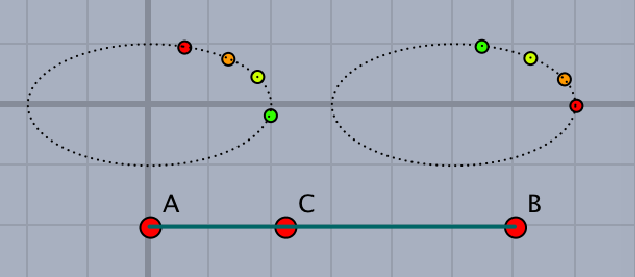
\includegraphics[bb=0.00 0.00 305.02 133.01,width=8cm]{Fig/numptcrv.pdf}
\end{center}

4行目で,2つのプロットデータの個数が同じであることを確かめている。

スライダを動かすと,10個おきのプロットデータに対応する点が描かれる。

\vspace{\baselineskip}
\hypertarget{paramoncrv}{}
\item[関数]  Paramoncrv(点の座標, 曲線の名前)
\item[機能]  曲線上の点のパラメータ値を返す。
\item[説明]  曲線は折れ線として描かれ,曲線上の各点はこの折れ線の節点を基準としたパラメータ値を持つ。パラメータ値は整数部分が節点の番号,小数部分が節間の位置を表す。

\vspace{\baselineskip}
【例】図のような点PからQに至る円周上の5等分点を節点とする折れ線cr1において,$n$番目の線分上の点は$n\leq t\leq n+1$の範囲のパラメータ値を持つ。

たとえば,図の点$\mathrm{A}$は2番目の線分上にあり,この値は

\begin{layer}{150}{0}
\putnotese{80}{0}{ %%% fig.tex 2016-5-3 12:50
%%% fig.sce 2016-5-3 12:50
{\unitlength=10mm%
\begin{picture}%
(   4.99000,   3.72000)(  -2.51000,  -0.69000)%
\special{pn 8}%
%
\special{pn 8}%
\special{pa 788 4}\special{pa 787 -4}\special{fp}\special{pa 785 -35}\special{pa 785 -43}\special{fp}%
\special{pa 783 -74}\special{pa 782 -82}\special{fp}\special{pa 778 -113}\special{pa 777 -121}\special{fp}%
\special{pa 771 -152}\special{pa 770 -160}\special{fp}\special{pa 764 -191}\special{pa 762 -198}\special{fp}%
\special{pa 752 -228}\special{pa 750 -236}\special{fp}\special{pa 740 -265}\special{pa 737 -273}\special{fp}%
\special{pa 726 -302}\special{pa 723 -309}\special{fp}\special{pa 710 -338}\special{pa 706 -345}\special{fp}%
\special{pa 693 -373}\special{pa 689 -380}\special{fp}\special{pa 673 -407}\special{pa 668 -414}\special{fp}%
\special{pa 652 -440}\special{pa 647 -447}\special{fp}\special{pa 629 -472}\special{pa 624 -478}\special{fp}%
\special{pa 604 -503}\special{pa 599 -509}\special{fp}\special{pa 579 -533}\special{pa 574 -539}\special{fp}%
\special{pa 551 -560}\special{pa 545 -566}\special{fp}\special{pa 523 -587}\special{pa 517 -593}\special{fp}%
\special{pa 493 -613}\special{pa 487 -618}\special{fp}\special{pa 461 -636}\special{pa 455 -641}\special{fp}%
\special{pa 430 -659}\special{pa 423 -664}\special{fp}\special{pa 396 -679}\special{pa 389 -683}\special{fp}%
\special{pa 361 -698}\special{pa 354 -702}\special{fp}\special{pa 326 -716}\special{pa 319 -719}\special{fp}%
\special{pa 290 -730}\special{pa 282 -733}\special{fp}\special{pa 253 -745}\special{pa 246 -748}\special{fp}%
\special{pa 216 -756}\special{pa 208 -758}\special{fp}\special{pa 178 -766}\special{pa 170 -768}\special{fp}%
\special{pa 139 -774}\special{pa 132 -776}\special{fp}\special{pa 101 -779}\special{pa 93 -780}\special{fp}%
\special{pa 62 -785}\special{pa 54 -785}\special{fp}\special{pa 22 -786}\special{pa 14 -786}\special{fp}%
\special{pa -17 -786}\special{pa -25 -786}\special{fp}\special{pa -56 -785}\special{pa -64 -784}\special{fp}%
\special{pa -95 -780}\special{pa -103 -779}\special{fp}\special{pa -134 -775}\special{pa -142 -774}\special{fp}%
\special{pa -172 -767}\special{pa -180 -765}\special{fp}\special{pa -211 -757}\special{pa -218 -755}\special{fp}%
\special{pa -248 -747}\special{pa -256 -744}\special{fp}\special{pa -285 -732}\special{pa -292 -729}\special{fp}%
\special{pa -321 -718}\special{pa -329 -715}\special{fp}\special{pa -357 -701}\special{pa -364 -697}\special{fp}%
\special{pa -391 -682}\special{pa -398 -678}\special{fp}\special{pa -425 -662}\special{pa -432 -658}\special{fp}%
\special{pa -457 -639}\special{pa -463 -635}\special{fp}\special{pa -489 -616}\special{pa -495 -611}\special{fp}%
\special{pa -519 -591}\special{pa -525 -586}\special{fp}\special{pa -547 -564}\special{pa -553 -559}\special{fp}%
\special{pa -576 -537}\special{pa -581 -531}\special{fp}\special{pa -601 -507}\special{pa -606 -501}\special{fp}%
\special{pa -626 -477}\special{pa -631 -470}\special{fp}\special{pa -649 -445}\special{pa -653 -438}\special{fp}%
\special{pa -670 -411}\special{pa -674 -405}\special{fp}\special{pa -690 -378}\special{pa -694 -371}\special{fp}%
\special{pa -707 -343}\special{pa -711 -335}\special{fp}\special{pa -724 -307}\special{pa -727 -300}\special{fp}%
\special{pa -738 -271}\special{pa -741 -263}\special{fp}\special{pa -751 -233}\special{pa -753 -226}\special{fp}%
\special{pa -762 -196}\special{pa -764 -188}\special{fp}\special{pa -770 -157}\special{pa -772 -149}\special{fp}%
\special{pa -778 -119}\special{pa -779 -111}\special{fp}\special{pa -782 -80}\special{pa -783 -72}\special{fp}%
\special{pa -785 -41}\special{pa -785 -33}\special{fp}\special{pa -787 -1}\special{pa -787 7}\special{fp}%
\special{pa -785 38}\special{pa -785 46}\special{fp}\special{pa -783 77}\special{pa -782 85}\special{fp}%
\special{pa -778 116}\special{pa -777 124}\special{fp}\special{pa -771 154}\special{pa -769 162}\special{fp}%
\special{pa -763 193}\special{pa -761 201}\special{fp}\special{pa -751 230}\special{pa -749 238}\special{fp}%
\special{pa -739 268}\special{pa -737 275}\special{fp}\special{pn 8}%
\special{pa 737 275}\special{pa 739 268}\special{fp}\special{pa 749 238}\special{pa 752 230}\special{fp}%
\special{pa 762 200}\special{pa 764 192}\special{fp}\special{pa 769 161}\special{pa 771 153}\special{fp}%
\special{pa 777 122}\special{pa 778 114}\special{fp}\special{pa 782 83}\special{pa 783 75}\special{fp}%
\special{pa 785 44}\special{pa 785 36}\special{fp}\special{pa 787 4}\special{pa 788 -4}\special{fp}%
\special{pn 8}%
\special{pa 787 0}\special{pa 637 -463}\special{pa 243 -749}\special{pa -243 -749}%
\special{pa -637 -463}\special{pa -787 0}%
\special{fp}%
\special{pn 5}%
\special{pa 483 -599}\special{pa 475 -604}\special{pa 465 -604}\special{pa 457 -600}%
\special{pa 451 -593}\special{pa 449 -584}\special{pa 452 -575}\special{pa 459 -568}%
\special{pa 468 -565}\special{pa 477 -567}\special{pa 484 -573}\special{pa 488 -581}%
\special{pa 488 -591}\special{pa 483 -599}\special{sh 1}\special{fp}%
\special{pa 801 -14}\special{pa 793 -19}\special{pa 784 -19}\special{pa 775 -15}\special{pa 769 -8}%
\special{pa 768 1}\special{pa 771 10}\special{pa 777 17}\special{pa 786 20}\special{pa 795 18}%
\special{pa 803 12}\special{pa 807 4}\special{pa 806 -6}\special{pa 801 -14}\special{sh 1}\special{fp}%
\special{pa -773 -14}\special{pa -782 -19}\special{pa -791 -19}\special{pa -800 -15}%
\special{pa -805 -8}\special{pa -807 1}\special{pa -804 10}\special{pa -798 17}\special{pa -789 20}%
\special{pa -779 18}\special{pa -772 12}\special{pa -768 4}\special{pa -769 -6}\special{pa -773 -14}%
\special{sh 1}\special{fp}%
\special{pn 8}%
\settowidth{\Width}{P}\setlength{\Width}{0\Width}%
\settoheight{\Height}{P}\settodepth{\Depth}{P}\setlength{\Height}{-\Height}%
\put(2.0500,-0.0500){\hspace*{\Width}\raisebox{\Height}{P}}%
%
%
\settowidth{\Width}{Q}\setlength{\Width}{-1\Width}%
\settoheight{\Height}{Q}\settodepth{\Depth}{Q}\setlength{\Height}{-\Height}%
\put(-2.0500,-0.0500){\hspace*{\Width}\raisebox{\Height}{Q}}%
%
%
\settowidth{\Width}{A}\setlength{\Width}{0\Width}%
\settoheight{\Height}{A}\settodepth{\Depth}{A}\setlength{\Height}{\Depth}%
\put(1.2409,1.5359){\hspace*{\Width}\raisebox{\Height}{A}}%
%
%
\special{pn 8}%
\special{pa -988 0}\special{pa 937 0}%
\special{fp}%
\special{pn 8}%
\special{pa 901 24}\special{pa 976 0}\special{pa 901 -24}\special{pa 901 0}\special{pa 901 24}%
\special{sh 1}\special{ip}%
\special{pn 1}%
\special{pa 901 24}\special{pa 976 0}\special{pa 901 -24}\special{pa 901 0}\special{pa 901 24}%
\special{pa 976 0}%
\special{fp}%
\special{pn 8}%
\special{pn 8}%
\special{pa 0 272}\special{pa 0 -1154}%
\special{fp}%
\special{pn 8}%
\special{pa 24 -1118}\special{pa 0 -1193}\special{pa -24 -1118}\special{pa 0 -1118}%
\special{pa 24 -1118}\special{sh 1}\special{ip}%
\special{pn 1}%
\special{pa 24 -1118}\special{pa 0 -1193}\special{pa -24 -1118}\special{pa 0 -1118}%
\special{pa 24 -1118}\special{pa 0 -1193}%
\special{fp}%
\special{pn 8}%
\settowidth{\Width}{$x$}\setlength{\Width}{0\Width}%
\settoheight{\Height}{$x$}\settodepth{\Depth}{$x$}\setlength{\Height}{-0.5\Height}\setlength{\Depth}{0.5\Depth}\addtolength{\Height}{\Depth}%
\put(2.5300,0.0000){\hspace*{\Width}\raisebox{\Height}{$x$}}%
%
%
\settowidth{\Width}{$y$}\setlength{\Width}{-0.5\Width}%
\settoheight{\Height}{$y$}\settodepth{\Depth}{$y$}\setlength{\Height}{\Depth}%
\put(0.0000,3.0800){\hspace*{\Width}\raisebox{\Height}{$y$}}%
%
%
\settowidth{\Width}{O}\setlength{\Width}{0\Width}%
\settoheight{\Height}{O}\settodepth{\Depth}{O}\setlength{\Height}{-\Height}%
\put(0.0500,-0.0500){\hspace*{\Width}\raisebox{\Height}{O}}%
%
%
\end{picture}}%}
\end{layer}

\begin{verbatim}
   println(Paramoncrv(A.xy,"cr1"));
\end{verbatim}  
    
によってコンソールに表示される。(たとえば2.45)。

点Aの位置を動かすとパラメータ値は変わる。

\vspace{20mm}
\begin{flushright}  \hyperlink{functionlist}{$\Rightarrow$関数一覧}\end{flushright}


\vspace{\baselineskip}
\hypertarget{pointoncrv}{}
\item[関数]  Pointoncrv(点のパラメータ値, PD)
\item[機能]  曲線上のパラメータ値を持つ点の座標を返す。
\item[説明]  曲線(折れ線)上の節点を基準としたパラメータ値により点の位置が定まる。

\vspace{\baselineskip}
【例】図のような点$\mathrm{P}$から$\mathrm{Q}$に至る半円周上の5等分点を節点とする折れ線cr1において,パラメータ値$4.5$を持つ点$\mathrm{A}$は4番目の線分の中点である。したがって

\begin{verbatim}
    Circledata("0",[[0,0],[2,0]],["do"]);
    Circledata("1",[[0,0],[2,0]],["Num=5","Rng=[0,pi]"]);
    tmp=Pointoncurve(4.5,"cr1");
    Pointdata("1",tmp,["Size=3"]);
    Letter([tmp,"nw","A",[2,0],"se","P",[-2,0],"sw","Q"]);
\end{verbatim}
    
によって,点Aを中点に置くことができる。

\vspace{\baselineskip}
 \begin{center} \scalebox{0.9}{%%% fig.tex 2016-5-3 14:0
%%% fig.sce 2016-5-3 14:0
{\unitlength=10mm%
\begin{picture}%
(   4.99000,   3.72000)(  -2.51000,  -0.69000)%
\special{pn 8}%
%
\special{pn 8}%
\special{pa 788 4}\special{pa 787 -4}\special{fp}\special{pa 785 -35}\special{pa 785 -43}\special{fp}%
\special{pa 783 -74}\special{pa 782 -82}\special{fp}\special{pa 778 -113}\special{pa 777 -121}\special{fp}%
\special{pa 771 -152}\special{pa 770 -160}\special{fp}\special{pa 764 -191}\special{pa 762 -198}\special{fp}%
\special{pa 752 -228}\special{pa 750 -236}\special{fp}\special{pa 740 -265}\special{pa 737 -273}\special{fp}%
\special{pa 726 -302}\special{pa 723 -309}\special{fp}\special{pa 710 -338}\special{pa 706 -345}\special{fp}%
\special{pa 693 -373}\special{pa 689 -380}\special{fp}\special{pa 673 -407}\special{pa 668 -414}\special{fp}%
\special{pa 652 -440}\special{pa 647 -447}\special{fp}\special{pa 629 -472}\special{pa 624 -478}\special{fp}%
\special{pa 604 -503}\special{pa 599 -509}\special{fp}\special{pa 579 -533}\special{pa 574 -539}\special{fp}%
\special{pa 551 -560}\special{pa 545 -566}\special{fp}\special{pa 523 -587}\special{pa 517 -593}\special{fp}%
\special{pa 493 -613}\special{pa 487 -618}\special{fp}\special{pa 461 -636}\special{pa 455 -641}\special{fp}%
\special{pa 430 -659}\special{pa 423 -664}\special{fp}\special{pa 396 -679}\special{pa 389 -683}\special{fp}%
\special{pa 361 -698}\special{pa 354 -702}\special{fp}\special{pa 326 -716}\special{pa 319 -719}\special{fp}%
\special{pa 290 -730}\special{pa 282 -733}\special{fp}\special{pa 253 -745}\special{pa 246 -748}\special{fp}%
\special{pa 216 -756}\special{pa 208 -758}\special{fp}\special{pa 178 -766}\special{pa 170 -768}\special{fp}%
\special{pa 139 -774}\special{pa 132 -776}\special{fp}\special{pa 101 -779}\special{pa 93 -780}\special{fp}%
\special{pa 62 -785}\special{pa 54 -785}\special{fp}\special{pa 22 -786}\special{pa 14 -786}\special{fp}%
\special{pa -17 -786}\special{pa -25 -786}\special{fp}\special{pa -56 -785}\special{pa -64 -784}\special{fp}%
\special{pa -95 -780}\special{pa -103 -779}\special{fp}\special{pa -134 -775}\special{pa -142 -774}\special{fp}%
\special{pa -172 -767}\special{pa -180 -765}\special{fp}\special{pa -211 -757}\special{pa -218 -755}\special{fp}%
\special{pa -248 -747}\special{pa -256 -744}\special{fp}\special{pa -285 -732}\special{pa -292 -729}\special{fp}%
\special{pa -321 -718}\special{pa -329 -715}\special{fp}\special{pa -357 -701}\special{pa -364 -697}\special{fp}%
\special{pa -391 -682}\special{pa -398 -678}\special{fp}\special{pa -425 -662}\special{pa -432 -658}\special{fp}%
\special{pa -457 -639}\special{pa -463 -635}\special{fp}\special{pa -489 -616}\special{pa -495 -611}\special{fp}%
\special{pa -519 -591}\special{pa -525 -586}\special{fp}\special{pa -547 -564}\special{pa -553 -559}\special{fp}%
\special{pa -576 -537}\special{pa -581 -531}\special{fp}\special{pa -601 -507}\special{pa -606 -501}\special{fp}%
\special{pa -626 -477}\special{pa -631 -470}\special{fp}\special{pa -649 -445}\special{pa -653 -438}\special{fp}%
\special{pa -670 -411}\special{pa -674 -405}\special{fp}\special{pa -690 -378}\special{pa -694 -371}\special{fp}%
\special{pa -707 -343}\special{pa -711 -335}\special{fp}\special{pa -724 -307}\special{pa -727 -300}\special{fp}%
\special{pa -738 -271}\special{pa -741 -263}\special{fp}\special{pa -751 -233}\special{pa -753 -226}\special{fp}%
\special{pa -762 -196}\special{pa -764 -188}\special{fp}\special{pa -770 -157}\special{pa -772 -149}\special{fp}%
\special{pa -778 -119}\special{pa -779 -111}\special{fp}\special{pa -782 -80}\special{pa -783 -72}\special{fp}%
\special{pa -785 -41}\special{pa -785 -33}\special{fp}\special{pa -787 -1}\special{pa -787 7}\special{fp}%
\special{pa -785 38}\special{pa -785 46}\special{fp}\special{pa -783 77}\special{pa -782 85}\special{fp}%
\special{pa -778 116}\special{pa -777 124}\special{fp}\special{pa -771 154}\special{pa -769 162}\special{fp}%
\special{pa -763 193}\special{pa -761 201}\special{fp}\special{pa -751 230}\special{pa -749 238}\special{fp}%
\special{pa -739 268}\special{pa -737 275}\special{fp}\special{pn 8}%
\special{pa 737 275}\special{pa 739 268}\special{fp}\special{pa 749 238}\special{pa 752 230}\special{fp}%
\special{pa 762 200}\special{pa 764 192}\special{fp}\special{pa 769 161}\special{pa 771 153}\special{fp}%
\special{pa 777 122}\special{pa 778 114}\special{fp}\special{pa 782 83}\special{pa 783 75}\special{fp}%
\special{pa 785 44}\special{pa 785 36}\special{fp}\special{pa 787 4}\special{pa 788 -4}\special{fp}%
\special{pn 8}%
\special{pa 787 0}\special{pa 637 -463}\special{pa 243 -749}\special{pa -243 -749}%
\special{pa -637 -463}\special{pa -787 0}%
\special{fp}%
\special{pn 5}%
\special{pa -426 -620}\special{pa -434 -625}\special{pa -444 -625}\special{pa -452 -621}%
\special{pa -458 -614}\special{pa -460 -605}\special{pa -457 -596}\special{pa -450 -589}%
\special{pa -441 -586}\special{pa -432 -588}\special{pa -425 -594}\special{pa -421 -602}%
\special{pa -421 -612}\special{pa -426 -620}\special{sh 1}\special{fp}%
\special{pa 801 -14}\special{pa 793 -19}\special{pa 784 -19}\special{pa 775 -15}\special{pa 769 -8}%
\special{pa 768 1}\special{pa 771 10}\special{pa 777 17}\special{pa 786 20}\special{pa 795 18}%
\special{pa 803 12}\special{pa 807 4}\special{pa 806 -6}\special{pa 801 -14}\special{sh 1}\special{fp}%
\special{pa -773 -14}\special{pa -782 -19}\special{pa -791 -19}\special{pa -800 -15}%
\special{pa -805 -8}\special{pa -807 1}\special{pa -804 10}\special{pa -798 17}\special{pa -789 20}%
\special{pa -779 18}\special{pa -772 12}\special{pa -768 4}\special{pa -769 -6}\special{pa -773 -14}%
\special{sh 1}\special{fp}%
\special{pn 8}%
\settowidth{\Width}{P}\setlength{\Width}{0\Width}%
\settoheight{\Height}{P}\settodepth{\Depth}{P}\setlength{\Height}{-\Height}%
\put(2.0500,-0.0500){\hspace*{\Width}\raisebox{\Height}{P}}%
%
%
\settowidth{\Width}{Q}\setlength{\Width}{-1\Width}%
\settoheight{\Height}{Q}\settodepth{\Depth}{Q}\setlength{\Height}{-\Height}%
\put(-2.0500,-0.0500){\hspace*{\Width}\raisebox{\Height}{Q}}%
%
%
\settowidth{\Width}{A}\setlength{\Width}{-1\Width}%
\settoheight{\Height}{A}\settodepth{\Depth}{A}\setlength{\Height}{\Depth}%
\put(-1.1680,1.5888){\hspace*{\Width}\raisebox{\Height}{A}}%
%
%
\special{pn 8}%
\special{pa -988 0}\special{pa 937 0}%
\special{fp}%
\special{pn 8}%
\special{pa 901 24}\special{pa 976 0}\special{pa 901 -24}\special{pa 901 0}\special{pa 901 24}%
\special{sh 1}\special{ip}%
\special{pn 1}%
\special{pa 901 24}\special{pa 976 0}\special{pa 901 -24}\special{pa 901 0}\special{pa 901 24}%
\special{pa 976 0}%
\special{fp}%
\special{pn 8}%
\special{pn 8}%
\special{pa 0 272}\special{pa 0 -1154}%
\special{fp}%
\special{pn 8}%
\special{pa 24 -1118}\special{pa 0 -1193}\special{pa -24 -1118}\special{pa 0 -1118}%
\special{pa 24 -1118}\special{sh 1}\special{ip}%
\special{pn 1}%
\special{pa 24 -1118}\special{pa 0 -1193}\special{pa -24 -1118}\special{pa 0 -1118}%
\special{pa 24 -1118}\special{pa 0 -1193}%
\special{fp}%
\special{pn 8}%
\settowidth{\Width}{$x$}\setlength{\Width}{0\Width}%
\settoheight{\Height}{$x$}\settodepth{\Depth}{$x$}\setlength{\Height}{-0.5\Height}\setlength{\Depth}{0.5\Depth}\addtolength{\Height}{\Depth}%
\put(2.5300,0.0000){\hspace*{\Width}\raisebox{\Height}{$x$}}%
%
%
\settowidth{\Width}{$y$}\setlength{\Width}{-0.5\Width}%
\settoheight{\Height}{$y$}\settodepth{\Depth}{$y$}\setlength{\Height}{\Depth}%
\put(0.0000,3.0800){\hspace*{\Width}\raisebox{\Height}{$y$}}%
%
%
\settowidth{\Width}{O}\setlength{\Width}{0\Width}%
\settoheight{\Height}{O}\settodepth{\Depth}{O}\setlength{\Height}{-\Height}%
\put(0.0500,-0.0500){\hspace*{\Width}\raisebox{\Height}{O}}%
%
%
\end{picture}}%} \end{center}

%\vspace{\baselineskip}
\hypertarget{ptcrv}{}
\item[関数]  Ptcrv(n,プロットデータ)
\item[機能]  曲線プロットデータのn 番目の節点を返す
\item[説明]  Cindyscript の PD\_n と同じ

\vspace{\baselineskip}
【例】楕円上の点で分割する。あからじめ必要な点を作図しておく。

\begin{layer}{150}{0}
\putnotese{70}{10}{ %%% test.tex 2014-12-3 14:24
%%% test.sce 2014-12-3 14:24
{\unitlength=6mm%
\begin{picture}%
(  10.00000,   8.00000)(  -5.00000,  -4.00000)%
\special{pn 8}%
%
\special{pa 829 -343}\special{pa 792 -334}\special{fp}\special{pa 754 -325}\special{pa 717 -316}\special{fp}%
\special{pa 679 -307}\special{pa 642 -298}\special{fp}\special{pa 604 -290}\special{pa 567 -281}\special{fp}%
\special{pa 530 -272}\special{pa 492 -263}\special{fp}\special{pa 455 -254}\special{pa 417 -246}\special{fp}%
\special{pa 380 -237}\special{pa 342 -228}\special{fp}\special{pa 305 -219}\special{pa 267 -210}\special{fp}%
\special{pa 230 -201}\special{pa 193 -193}\special{fp}\special{pa 155 -184}\special{pa 118 -175}\special{fp}%
\special{pa 80 -166}\special{pa 43 -157}\special{fp}\special{pa 5 -149}\special{pa -32 -140}\special{fp}%
\special{pa -70 -131}\special{pa -107 -122}\special{fp}\special{pa -144 -113}\special{pa -182 -105}\special{fp}%
\special{pa -219 -96}\special{pa -257 -87}\special{fp}\special{pa -294 -78}\special{pa -332 -69}\special{fp}%
\special{pa -369 -60}\special{pa -407 -52}\special{fp}\special{pa -444 -43}\special{pa -481 -34}\special{fp}%
\special{pa -519 -25}\special{pa -556 -16}\special{fp}\special{pa -594 -8}\special{pa -626 0}\special{pa -621 -2}\special{fp}%
\special{pa -587 -19}\special{pa -552 -36}\special{fp}\special{pa -517 -53}\special{pa -483 -70}\special{fp}%
\special{pa -448 -86}\special{pa -414 -103}\special{fp}\special{pa -379 -120}\special{pa -344 -137}\special{fp}%
\special{pa -310 -154}\special{pa -275 -170}\special{fp}\special{pa -241 -187}\special{pa -206 -204}\special{fp}%
\special{pa -171 -221}\special{pa -137 -238}\special{fp}\special{pa -102 -255}\special{pa -68 -271}\special{fp}%
\special{pa -33 -288}\special{pa 2 -305}\special{fp}\special{pa 36 -322}\special{pa 71 -339}\special{fp}%
\special{pa 105 -355}\special{pa 140 -372}\special{fp}\special{pa 175 -389}\special{pa 209 -406}\special{fp}%
\special{pa 244 -423}\special{pa 278 -440}\special{fp}\special{pa 313 -456}\special{pa 348 -473}\special{fp}%
\special{pa 382 -490}\special{pa 417 -507}\special{fp}\special{pa 451 -524}\special{pa 486 -540}\special{fp}%
\special{pa 521 -557}\special{pa 555 -574}\special{fp}%
%
\special{pn 24}%
\special{pa 826 -341}\special{pa 826 -341}\special{pa 796 -380}\special{pa 763 -417}%
\special{pa 726 -452}\special{pa 687 -485}\special{pa 645 -517}\special{pa 601 -546}%
\special{pa 555 -573}%
\special{fp}%
\special{pn 8}%
\special{pa 826 -341}\special{pa 796 -380}\special{pa 763 -417}\special{pa 726 -452}%
\special{pa 687 -485}\special{pa 645 -517}\special{pa 601 -546}\special{pa 555 -573}%
\special{pa -626 0}\special{pa 829 -343}\special{pa 826 -341}\special{sh 0.1}\special{ip}%
\special{pa 669 -544}\special{pa 555 -574}\special{pa 630 -483}\special{pa 650 -513}%
\special{pa 669 -544}\special{sh 1}\special{ip}%
\special{pn 8}%
\special{pa 669 -544}\special{pa 555 -574}\special{pa 630 -483}\special{pa 650 -513}%
\special{pa 669 -544}%
\special{fp}%
\special{pn 8}%
\settowidth{\Width}{A}\setlength{\Width}{0\Width}%
\settoheight{\Height}{A}\settodepth{\Depth}{A}\setlength{\Height}{\Depth}%
\put(3.5600,1.5000){\hspace*{\Width}\raisebox{\Height}{A}}%
%
%
\settowidth{\Width}{B}\setlength{\Width}{0\Width}%
\settoheight{\Height}{B}\settodepth{\Depth}{B}\setlength{\Height}{\Depth}%
\put(2.4000,2.4800){\hspace*{\Width}\raisebox{\Height}{B}}%
%
%
\settowidth{\Width}{F}\setlength{\Width}{-0.5\Width}%
\settoheight{\Height}{F}\settodepth{\Depth}{F}\setlength{\Height}{-\Height}%
\put(-2.6500,-0.1500){\hspace*{\Width}\raisebox{\Height}{F}}%
%
%
\special{pa -615 -11}\special{pa -622 -15}\special{pa -630 -15}\special{pa -637 -11}%
\special{pa -641 -4}\special{pa -641 4}\special{pa -637 11}\special{pa -630 15}\special{pa -622 15}%
\special{pa -615 11}\special{pa -611 4}\special{pa -611 -4}\special{pa -615 -11}\special{sh 1}\special{fp}%
\special{pa 943 0}\special{pa 941 -44}\special{pa 935 -89}\special{pa 926 -133}\special{pa 913 -176}%
\special{pa 896 -219}\special{pa 876 -261}\special{pa 853 -302}\special{pa 826 -341}%
\special{pa 796 -380}\special{pa 763 -417}\special{pa 726 -452}\special{pa 687 -485}%
\special{pa 645 -517}\special{pa 601 -546}\special{pa 554 -573}\special{pa 505 -598}%
\special{pa 454 -621}\special{pa 401 -641}\special{pa 347 -659}\special{pa 291 -674}%
\special{pa 234 -686}\special{pa 177 -696}\special{pa 118 -703}\special{pa 59 -707}%
\special{pa 0 -709}\special{pa -59 -707}\special{pa -118 -703}\special{pa -177 -696}%
\special{pa -234 -686}\special{pa -291 -674}\special{pa -347 -659}\special{pa -401 -641}%
\special{pa -454 -621}\special{pa -505 -598}\special{pa -554 -573}\special{pa -601 -546}%
\special{pa -645 -517}\special{pa -687 -485}\special{pa -726 -452}\special{pa -763 -417}%
\special{pa -796 -380}\special{pa -826 -341}\special{pa -853 -302}\special{pa -876 -261}%
\special{pa -896 -219}\special{pa -913 -176}\special{pa -926 -133}\special{pa -935 -89}%
\special{pa -941 -44}\special{pa -943 0}\special{pa -941 44}\special{pa -935 89}\special{pa -926 133}%
\special{pa -913 176}\special{pa -896 219}\special{pa -876 261}\special{pa -853 302}%
\special{pa -826 341}\special{pa -796 380}\special{pa -763 417}\special{pa -726 452}%
\special{pa -687 485}\special{pa -645 517}\special{pa -601 546}\special{pa -554 573}%
\special{pa -505 598}\special{pa -454 621}\special{pa -401 641}\special{pa -347 659}%
\special{pa -291 674}\special{pa -234 686}\special{pa -177 696}\special{pa -118 703}%
\special{pa -59 707}\special{pa 0 709}\special{pa 59 707}\special{pa 118 703}\special{pa 177 696}%
\special{pa 234 686}\special{pa 291 674}\special{pa 347 659}\special{pa 401 641}\special{pa 454 621}%
\special{pa 505 598}\special{pa 554 573}\special{pa 601 546}\special{pa 645 517}\special{pa 687 485}%
\special{pa 726 452}\special{pa 763 417}\special{pa 796 380}\special{pa 826 341}\special{pa 853 302}%
\special{pa 876 261}\special{pa 896 219}\special{pa 913 176}\special{pa 926 133}\special{pa 935 89}%
\special{pa 941 44}\special{pa 943 0}%
\special{fp}%
\special{pa -1181 0}\special{pa 1181 0}%
\special{fp}%
\special{pa 0 945}\special{pa 0 -945}%
\special{fp}%
\settowidth{\Width}{$x$}\setlength{\Width}{0\Width}%
\settoheight{\Height}{$x$}\settodepth{\Depth}{$x$}\setlength{\Height}{-0.5\Height}\setlength{\Depth}{0.5\Depth}\addtolength{\Height}{\Depth}%
\put(5.0500,0.0000){\hspace*{\Width}\raisebox{\Height}{$x$}}%
%
%
\settowidth{\Width}{$y$}\setlength{\Width}{-0.5\Width}%
\settoheight{\Height}{$y$}\settodepth{\Depth}{$y$}\setlength{\Height}{\Depth}%
\put(0.0000,4.0500){\hspace*{\Width}\raisebox{\Height}{$y$}}%
%
%
\settowidth{\Width}{O}\setlength{\Width}{-1\Width}%
\settoheight{\Height}{O}\settodepth{\Depth}{O}\setlength{\Height}{-\Height}%
\put(-0.0500,-0.0500){\hspace*{\Width}\raisebox{\Height}{O}}%
%
%
\end{picture}}%}
\end{layer}
\begin{verbatim}
  Circledata([O,P],["do","Num=100","notex"]);
  Scaledata("1","crOP",4/3,1);
  F.xy=[-sqrt(7),0];
  A=Ptcrv(9,sc1);
  B=Ptcrv(16,sc1);
  Listplot("1",[A,F,B],["da"]);
  Partcrv("1",A,B,"sc1",["dr,3"]);
  Shade(["part1","sg1"],0.1);
  Arrowhead(B,"sc1",[1.5]);
  Letter([A,"ne","A",B,"ne","B",F,"s2","F"]);
\end{verbatim}
   
%\begin{flushright}  \hyperlink{functionlist}{$\Rightarrow$関数一覧}\end{flushright}

\vspace{\baselineskip}
\hypertarget{ptstart}{}
\item[関数]  Ptstart(プロットデータ) , Ptend(プロットデータ)
\item[機能]  プロットデータの最初の点,最後の点を取得する。
\item[説明]  プロットデータの最初の点,最後の点の座標を返す。

\vspace{\baselineskip}
【例】定義域を限定したグラフの両端の点を取得し線分ABを引く。
\begin{verbatim}
  Deffun("f(x)",["regional(y)","y=x^2","y"]); 
  Plotdata("1","f(x)","x",["do"]);
  Plotdata("2","f(x)","x=[-1,2]");
  Lineplot("1",[Ptstart(gr2),Ptend(gr2)],["do"]);
  Listplot("1",[Ptstart(gr2),Ptend(gr2)]);
  Letter([A,"w2","A",B,"e2","B"]);
\end{verbatim}
\vspace{\baselineskip}
\begin{center} %%% ptstart.tex 2014-11-13 9:50
%%% ptcrv.sce 2014-11-12 22:40
{\unitlength=1cm%
\begin{picture}%
(   5.89000,   5.26000)(  -2.57000,  -0.54000)%
\special{pn 8}%
%
\special{pa -394 -394}\special{pa -370 -347}\special{pa -345 -303}\special{pa -321 -262}%
\special{pa -297 -224}\special{pa -273 -190}\special{pa -249 -158}\special{pa -225 -129}%
\special{pa -201 -102}\special{pa -177 -79}\special{pa -153 -59}\special{pa -129 -42}%
\special{pa -104 -28}\special{pa -80 -16}\special{pa -56 -8}\special{pa -32 -3}\special{pa -8 0}%
\special{pa 16 -1}\special{pa 40 -4}\special{pa 64 -10}\special{pa 88 -20}\special{pa 112 -32}%
\special{pa 137 -47}\special{pa 161 -66}\special{pa 185 -87}\special{pa 209 -111}%
\special{pa 233 -138}\special{pa 257 -168}\special{pa 281 -201}\special{pa 305 -237}%
\special{pa 329 -276}\special{pa 354 -317}\special{pa 378 -362}\special{pa 402 -410}%
\special{pa 426 -461}\special{pa 450 -514}\special{pa 474 -571}\special{pa 498 -630}%
\special{pa 522 -693}\special{pa 546 -758}\special{pa 570 -827}\special{pa 595 -898}%
\special{pa 619 -972}\special{pa 643 -1049}\special{pa 667 -1130}\special{pa 691 -1213}%
\special{pa 715 -1299}\special{pa 739 -1388}\special{pa 763 -1480}\special{pa 787 -1575}%
\special{fp}%
\special{pn 8}%
\special{pa -856 -1862}\special{pa -854 -1854}\special{fp}\special{pa -847 -1824}\special{pa -845 -1816}\special{fp}%
\special{pa -838 -1786}\special{pa -836 -1778}\special{fp}\special{pa -829 -1747}\special{pa -827 -1740}\special{fp}%
\special{pa -820 -1709}\special{pa -818 -1701}\special{fp}\special{pa -811 -1671}\special{pa -809 -1663}\special{fp}%
\special{pa -801 -1633}\special{pa -800 -1625}\special{fp}\special{pa -792 -1595}\special{pa -790 -1587}\special{fp}%
\special{pa -783 -1557}\special{pa -781 -1549}\special{fp}\special{pa -773 -1519}\special{pa -771 -1511}\special{fp}%
\special{pa -763 -1481}\special{pa -761 -1473}\special{fp}\special{pa -753 -1443}\special{pa -751 -1435}\special{fp}%
\special{pa -743 -1405}\special{pa -741 -1397}\special{fp}\special{pa -733 -1367}\special{pa -731 -1359}\special{fp}%
\special{pa -723 -1329}\special{pa -721 -1321}\special{fp}\special{pa -713 -1291}\special{pa -710 -1283}\special{fp}%
\special{pa -702 -1253}\special{pa -700 -1245}\special{fp}\special{pa -691 -1215}\special{pa -689 -1208}\special{fp}%
\special{pa -681 -1177}\special{pa -679 -1170}\special{fp}\special{pa -670 -1140}\special{pa -667 -1132}\special{fp}%
\special{pa -658 -1102}\special{pa -656 -1095}\special{fp}\special{pa -647 -1065}\special{pa -645 -1057}\special{fp}%
\special{pa -636 -1027}\special{pa -633 -1019}\special{fp}\special{pa -624 -990}\special{pa -621 -982}\special{fp}%
\special{pa -612 -952}\special{pa -609 -945}\special{fp}\special{pa -600 -915}\special{pa -597 -907}\special{fp}%
\special{pa -588 -877}\special{pa -585 -870}\special{fp}\special{pa -575 -840}\special{pa -572 -833}\special{fp}%
\special{pa -562 -803}\special{pa -559 -796}\special{fp}\special{pa -549 -766}\special{pa -546 -759}\special{fp}%
\special{pa -536 -729}\special{pa -533 -722}\special{fp}\special{pa -522 -693}\special{pa -519 -685}\special{fp}%
\special{pa -508 -656}\special{pa -505 -648}\special{fp}\special{pa -494 -619}\special{pa -491 -612}\special{fp}%
\special{pa -479 -583}\special{pa -476 -576}\special{fp}\special{pa -463 -547}\special{pa -460 -539}\special{fp}%
\special{pa -448 -511}\special{pa -445 -503}\special{fp}\special{pa -432 -475}\special{pa -429 -468}\special{fp}%
\special{pa -415 -439}\special{pa -412 -432}\special{fp}\special{pa -399 -404}\special{pa -395 -397}\special{fp}%
\special{pa -380 -369}\special{pa -377 -362}\special{fp}\special{pa -362 -334}\special{pa -358 -327}\special{fp}%
\special{pa -343 -300}\special{pa -339 -293}\special{fp}\special{pa -323 -266}\special{pa -319 -259}\special{fp}%
\special{pa -303 -233}\special{pa -298 -226}\special{fp}\special{pa -280 -200}\special{pa -275 -194}\special{fp}%
\special{pa -257 -168}\special{pa -253 -162}\special{fp}\special{pa -232 -138}\special{pa -227 -132}\special{fp}%
\special{pa -206 -109}\special{pa -201 -103}\special{fp}\special{pa -178 -82}\special{pa -172 -76}\special{fp}%
\special{pa -148 -57}\special{pa -141 -52}\special{fp}\special{pa -116 -34}\special{pa -109 -30}\special{fp}%
\special{pa -80 -17}\special{pa -73 -14}\special{fp}\special{pa -43 -6}\special{pa -35 -4}\special{fp}%
\special{pa -4 -1}\special{pa 4 -1}\special{fp}\special{pa 35 -4}\special{pa 43 -5}\special{fp}%
\special{pa 73 -14}\special{pa 81 -16}\special{fp}\special{pa 108 -31}\special{pa 115 -35}\special{fp}%
\special{pa 141 -52}\special{pa 148 -57}\special{fp}\special{pa 172 -76}\special{pa 178 -81}\special{fp}%
\special{pa 200 -103}\special{pa 206 -109}\special{fp}\special{pa 227 -132}\special{pa 232 -138}\special{fp}%
\special{pa 252 -162}\special{pa 257 -169}\special{fp}\special{pa 275 -194}\special{pa 280 -200}\special{fp}%
\special{pa 298 -226}\special{pa 302 -233}\special{fp}\special{pa 319 -259}\special{pa 323 -266}\special{fp}%
\special{pa 339 -293}\special{pa 343 -300}\special{fp}\special{pa 359 -327}\special{pa 363 -334}\special{fp}%
\special{pa 377 -362}\special{pa 380 -369}\special{fp}\special{pa 395 -397}\special{pa 398 -404}\special{fp}%
\special{pa 412 -432}\special{pa 416 -439}\special{fp}\special{pa 428 -468}\special{pa 432 -475}\special{fp}%
\special{pa 445 -503}\special{pa 448 -511}\special{fp}\special{pa 461 -539}\special{pa 464 -547}\special{fp}%
\special{pa 475 -576}\special{pa 479 -583}\special{fp}\special{pa 490 -612}\special{pa 493 -619}\special{fp}%
\special{pa 505 -648}\special{pa 508 -656}\special{fp}\special{pa 519 -685}\special{pa 522 -693}\special{fp}%
\special{pa 533 -722}\special{pa 535 -729}\special{fp}\special{pa 546 -759}\special{pa 549 -766}\special{fp}%
\special{pa 559 -796}\special{pa 562 -803}\special{fp}\special{pa 572 -833}\special{pa 575 -840}\special{fp}%
\special{pa 585 -870}\special{pa 587 -878}\special{fp}\special{pa 598 -907}\special{pa 600 -915}\special{fp}%
\special{pa 609 -945}\special{pa 612 -952}\special{fp}\special{pa 621 -982}\special{pa 624 -990}\special{fp}%
\special{pa 633 -1019}\special{pa 636 -1027}\special{fp}\special{pa 645 -1057}\special{pa 647 -1065}\special{fp}%
\special{pa 656 -1095}\special{pa 658 -1102}\special{fp}\special{pa 667 -1132}\special{pa 669 -1140}\special{fp}%
\special{pa 678 -1170}\special{pa 681 -1178}\special{fp}\special{pa 689 -1208}\special{pa 692 -1215}\special{fp}%
\special{pa 700 -1245}\special{pa 702 -1253}\special{fp}\special{pa 710 -1283}\special{pa 713 -1291}\special{fp}%
\special{pa 721 -1321}\special{pa 723 -1329}\special{fp}\special{pa 731 -1359}\special{pa 733 -1367}\special{fp}%
\special{pa 741 -1397}\special{pa 744 -1405}\special{fp}\special{pa 751 -1435}\special{pa 753 -1443}\special{fp}%
\special{pa 761 -1473}\special{pa 763 -1481}\special{fp}\special{pa 771 -1511}\special{pa 773 -1519}\special{fp}%
\special{pa 781 -1549}\special{pa 783 -1557}\special{fp}\special{pa 790 -1587}\special{pa 792 -1595}\special{fp}%
\special{pa 800 -1625}\special{pa 802 -1633}\special{fp}\special{pa 809 -1663}\special{pa 811 -1671}\special{fp}%
\special{pa 818 -1701}\special{pa 820 -1709}\special{fp}\special{pa 827 -1740}\special{pa 829 -1747}\special{fp}%
\special{pa 837 -1778}\special{pa 838 -1786}\special{fp}\special{pa 845 -1816}\special{pa 847 -1824}\special{fp}%
\special{pa 854 -1854}\special{pa 856 -1862}\special{fp}\special{pn 8}%
\special{pn 8}%
\special{pa -1003 215}\special{pa -997 210}\special{fp}\special{pa -975 187}\special{pa -969 182}\special{fp}%
\special{pa -947 159}\special{pa -941 154}\special{fp}\special{pa -919 131}\special{pa -913 126}\special{fp}%
\special{pa -891 103}\special{pa -885 98}\special{fp}\special{pa -863 76}\special{pa -857 70}\special{fp}%
\special{pa -835 48}\special{pa -829 42}\special{fp}\special{pa -807 20}\special{pa -801 14}\special{fp}%
\special{pa -779 -8}\special{pa -773 -14}\special{fp}\special{pa -751 -36}\special{pa -745 -42}\special{fp}%
\special{pa -723 -64}\special{pa -717 -70}\special{fp}\special{pa -695 -92}\special{pa -689 -98}\special{fp}%
\special{pa -667 -120}\special{pa -661 -126}\special{fp}\special{pa -639 -148}\special{pa -633 -154}\special{fp}%
\special{pa -611 -176}\special{pa -605 -182}\special{fp}\special{pa -583 -204}\special{pa -577 -210}\special{fp}%
\special{pa -555 -232}\special{pa -549 -238}\special{fp}\special{pa -527 -260}\special{pa -521 -266}\special{fp}%
\special{pa -499 -288}\special{pa -493 -294}\special{fp}\special{pa -471 -316}\special{pa -465 -322}\special{fp}%
\special{pa -443 -344}\special{pa -437 -350}\special{fp}\special{pa -415 -372}\special{pa -409 -378}\special{fp}%
\special{pa -387 -400}\special{pa -382 -406}\special{fp}\special{pa -359 -428}\special{pa -354 -434}\special{fp}%
\special{pa -331 -456}\special{pa -326 -462}\special{fp}\special{pa -303 -484}\special{pa -298 -490}\special{fp}%
\special{pa -275 -512}\special{pa -270 -518}\special{fp}\special{pa -247 -540}\special{pa -242 -546}\special{fp}%
\special{pa -219 -568}\special{pa -214 -574}\special{fp}\special{pa -191 -596}\special{pa -186 -602}\special{fp}%
\special{pa -163 -624}\special{pa -158 -630}\special{fp}\special{pa -135 -652}\special{pa -130 -658}\special{fp}%
\special{pa -107 -680}\special{pa -102 -686}\special{fp}\special{pa -79 -708}\special{pa -74 -714}\special{fp}%
\special{pa -51 -736}\special{pa -46 -742}\special{fp}\special{pa -23 -764}\special{pa -18 -770}\special{fp}%
\special{pa 5 -792}\special{pa 10 -798}\special{fp}\special{pa 33 -820}\special{pa 38 -826}\special{fp}%
\special{pa 61 -848}\special{pa 66 -854}\special{fp}\special{pa 89 -876}\special{pa 94 -882}\special{fp}%
\special{pa 117 -904}\special{pa 122 -910}\special{fp}\special{pa 145 -932}\special{pa 150 -938}\special{fp}%
\special{pa 173 -960}\special{pa 178 -966}\special{fp}\special{pa 201 -988}\special{pa 206 -994}\special{fp}%
\special{pa 228 -1016}\special{pa 234 -1022}\special{fp}\special{pa 256 -1044}\special{pa 262 -1050}\special{fp}%
\special{pa 284 -1072}\special{pa 290 -1078}\special{fp}\special{pa 312 -1100}\special{pa 318 -1106}\special{fp}%
\special{pa 340 -1128}\special{pa 346 -1133}\special{fp}\special{pa 368 -1156}\special{pa 374 -1161}\special{fp}%
\special{pa 396 -1184}\special{pa 402 -1189}\special{fp}\special{pa 424 -1212}\special{pa 430 -1217}\special{fp}%
\special{pa 452 -1240}\special{pa 458 -1245}\special{fp}\special{pa 480 -1268}\special{pa 486 -1273}\special{fp}%
\special{pa 508 -1296}\special{pa 514 -1301}\special{fp}\special{pa 536 -1324}\special{pa 542 -1329}\special{fp}%
\special{pa 564 -1352}\special{pa 570 -1357}\special{fp}\special{pa 592 -1380}\special{pa 598 -1385}\special{fp}%
\special{pa 620 -1408}\special{pa 626 -1413}\special{fp}\special{pa 648 -1436}\special{pa 654 -1441}\special{fp}%
\special{pa 676 -1464}\special{pa 682 -1469}\special{fp}\special{pa 704 -1492}\special{pa 710 -1497}\special{fp}%
\special{pa 732 -1520}\special{pa 738 -1525}\special{fp}\special{pa 760 -1548}\special{pa 766 -1553}\special{fp}%
\special{pa 788 -1576}\special{pa 794 -1581}\special{fp}\special{pa 816 -1604}\special{pa 822 -1609}\special{fp}%
\special{pa 844 -1632}\special{pa 850 -1637}\special{fp}\special{pa 872 -1660}\special{pa 878 -1665}\special{fp}%
\special{pa 900 -1688}\special{pa 906 -1693}\special{fp}\special{pa 928 -1716}\special{pa 934 -1721}\special{fp}%
\special{pa 956 -1744}\special{pa 962 -1749}\special{fp}\special{pa 984 -1771}\special{pa 990 -1777}\special{fp}%
\special{pa 1012 -1799}\special{pa 1018 -1805}\special{fp}\special{pa 1040 -1827}\special{pa 1046 -1833}\special{fp}%
\special{pa 1068 -1855}\special{pa 1074 -1861}\special{fp}\special{pn 8}%
\settowidth{\Width}{A}\setlength{\Width}{-1\Width}%
\settoheight{\Height}{A}\settodepth{\Depth}{A}\setlength{\Height}{-0.5\Height}\setlength{\Depth}{0.5\Depth}\addtolength{\Height}{\Depth}%
\put(-1.2000,1.0000){\hspace*{\Width}\raisebox{\Height}{A}}%
%
%
\settowidth{\Width}{B}\setlength{\Width}{0\Width}%
\settoheight{\Height}{B}\settodepth{\Depth}{B}\setlength{\Height}{-0.5\Height}\setlength{\Depth}{0.5\Depth}\addtolength{\Height}{\Depth}%
\put(2.1500,4.0000){\hspace*{\Width}\raisebox{\Height}{B}}%
%
%
\special{pa -394 -394}\special{pa 787 -1575}%
\special{fp}%
\special{pa -1012 0}\special{pa 1307 0}%
\special{fp}%
\special{pa 0 213}\special{pa 0 -1858}%
\special{fp}%
\settowidth{\Width}{$x$}\setlength{\Width}{0\Width}%
\settoheight{\Height}{$x$}\settodepth{\Depth}{$x$}\setlength{\Height}{-0.5\Height}\setlength{\Depth}{0.5\Depth}\addtolength{\Height}{\Depth}%
\put(3.3700,0.0000){\hspace*{\Width}\raisebox{\Height}{$x$}}%
%
%
\settowidth{\Width}{$y$}\setlength{\Width}{-0.5\Width}%
\settoheight{\Height}{$y$}\settodepth{\Depth}{$y$}\setlength{\Height}{\Depth}%
\put(0.0000,4.7700){\hspace*{\Width}\raisebox{\Height}{$y$}}%
%
%
\settowidth{\Width}{O}\setlength{\Width}{-1\Width}%
\settoheight{\Height}{O}\settodepth{\Depth}{O}\setlength{\Height}{-\Height}%
\put(-0.0500,-0.0500){\hspace*{\Width}\raisebox{\Height}{O}}%
%
%
\end{picture}}% \end{center}

\begin{flushright}  \hyperlink{functionlist}{$\Rightarrow$関数一覧}\end{flushright}
\vspace{\baselineskip}
\hypertarget{readoutdata}{}
\item[関数]  ReadOutData(ファイル名)
\item[機能]  外部データをプロットデータとして読み込む
\item[説明]  CやRなどで作成したKeTCindy形式のデータファイルを読み込む。

引数を省略した場合は,Fheadで定義したファイル名のテキストファイルから読み込む。

ファイル名にはコンマで区切ってパスを与えることができる。たとえば,

\verb|ReadOutData("/datafolder","file.txt"); |
      
KeTCindy形式のデータとは

 変数名// \\
 start//  (リストの始まり) \\
 [ , , ], …. // (個々のデータ2か3次元) \\
 … \\
 end// (リストの終わり) \\
 start// (次のリストの始まり) \\
    … \\
 end// \\
 変数名// \\
 start// \\
 … \\
 end// \\

の形式のテキストファイル。

\vspace{\baselineskip}
\hypertarget{writeoutdata}{}
\item[関数]  WriteOutData(ファイル名,PDリスト)
\item[機能]  外部データに書き出す
\item[説明]  プロットデータをKeTCindy形式のデータファイルに書き出す。出力先の 初期設定は作業フォルダ。

【例】 放物線と円のプロットデータを書き出す。

\begin{verbatim}
     Plotdata("1", "x^2","x");
     Circledata("1",[[0,0],[1,0]]);
     WriteOutData("figdata.txt",["gr1",gr1,"cr1",cr1]);
\end{verbatim}

書き出されたファイルの中身は次のようになっている。

\begin{verbatim}
gr1// 
start//
[[-2.68843,7.22765],[-2.51807,6.34067],・・,[-2.00698,4.02798]]//
[[-1.83662,3.37318],[-1.66626,2.77642],・・,[-1.15518,1.33443]]//
  以下,同様にプロットデータが続く
[[5.82965,33.98479]]//
end//
cr1//
start//
[[1,0],[0.99211,0.12533],[0.96858,0.24869],・・,[0.80902,0.58779]]//
  以下,同様にプロットデータが続く
[[0.87631,-0.48175],[0.92978,-0.36812],・・,[1,0]]//
end////
\end{verbatim}
\begin{flushright}  \hyperlink{functionlist}{$\Rightarrow$関数一覧}\end{flushright}

\vspace{\baselineskip}
\hypertarget{extractdata}{}
\item[関数]  Extractdata(データ名,属性)
\item[機能]  ReadOutData() で読み込んだデータに属性をつける。
\item[説明]  ReadOutData() で読み込んだデータには,線種などの属性がついていないので,そのままでは表示されない。そこで,この関数により属性をつけて表示する。
\begin{verbatim}
    ReadOutData("figdata.txt");
    Extractdata("gr1",["da"]);
\end{verbatim}

\end{description}
%\newpage
% ======== 計算 =======================
\subsection{計算}

\begin{description}

\hypertarget{derivative}{}
\item[関数]  Derivative(関数式 , 変数 , 値)
\item[機能]  関数の微分係数を求める
\item[説明]  関数式で与えられた関数の,「変数=値」における微分係数を求める。

値は,点の座標を用いることができる。点Aのx座標であれば, A.x とする。

\vspace{\baselineskip}
【例】3次曲線上の点Aで接線を引く。点A,Bは作図ツールで適当にとっておく。
\begin{verbatim}
    Deffun("f(x)",["regional(y)","y=x^3-4*x","y"]);
    coef=Derivative("f(x)","x",A.x);
    A.y=f(A.x);
    B.y=coef*(B.x-A.x)+A.y;
    Plotdata("1","f(x)","x",["Num=200"]);
    Lineplot([A,B]);
    Letter([A,"ne","A"]);
\end{verbatim}
%\vspace{\baselineskip}
    \begin{center} %%% test.tex 2014-10-22 20:20
%%% test.sce 2014-10-22 20:20
{\unitlength=5mm%
\begin{picture}%
(   8.00000,   8.00000)(  -4.00000,  -4.00000)%
\special{pn 8}%
%
\settowidth{\Width}{A}\setlength{\Width}{0\Width}%
\settoheight{\Height}{A}\settodepth{\Depth}{A}\setlength{\Height}{\Depth}%
\put(-0.9500,3.0500){\hspace*{\Width}\raisebox{\Height}{A}}%
%
%
\special{pa -469 787}\special{pa -463 709}\special{pa -455 611}\special{pa -447 518}%
\special{pa -439 430}\special{pa -431 345}\special{pa -423 265}\special{pa -415 189}%
\special{pa -408 117}\special{pa -400 49}\special{pa -392 -16}\special{pa -384 -76}%
\special{pa -376 -133}\special{pa -368 -186}\special{pa -360 -236}\special{pa -352 -282}%
\special{pa -344 -324}\special{pa -336 -364}\special{pa -328 -400}\special{pa -321 -432}%
\special{pa -313 -462}\special{pa -305 -489}\special{pa -297 -513}\special{pa -289 -533}%
\special{pa -281 -552}\special{pa -273 -567}\special{pa -265 -580}\special{pa -257 -590}%
\special{pa -249 -597}\special{pa -241 -603}\special{pa -233 -605}\special{pa -226 -606}%
\special{pa -218 -605}\special{pa -210 -601}\special{pa -202 -595}\special{pa -194 -587}%
\special{pa -186 -578}\special{pa -178 -567}\special{pa -170 -553}\special{pa -162 -539}%
\special{pa -154 -522}\special{pa -146 -505}\special{pa -138 -485}\special{pa -131 -465}%
\special{pa -123 -443}\special{pa -115 -420}\special{pa -107 -396}\special{pa -99 -371}%
\special{pa -91 -345}\special{pa -83 -318}\special{pa -75 -290}\special{pa -67 -261}%
\special{pa -59 -232}\special{pa -51 -202}\special{pa -44 -172}\special{pa -36 -141}%
\special{pa -28 -110}\special{pa -20 -79}\special{pa -12 -47}\special{pa -4 -16}\special{pa 4 16}%
\special{pa 12 47}\special{pa 20 79}\special{pa 28 110}\special{pa 36 141}\special{pa 44 172}%
\special{pa 51 202}\special{pa 59 232}\special{pa 67 261}\special{pa 75 290}\special{pa 83 318}%
\special{pa 91 345}\special{pa 99 371}\special{pa 107 396}\special{pa 115 420}\special{pa 123 443}%
\special{pa 131 465}\special{pa 138 485}\special{pa 146 505}\special{pa 154 522}\special{pa 162 539}%
\special{pa 170 553}\special{pa 178 567}\special{pa 186 578}\special{pa 194 587}\special{pa 202 595}%
\special{pa 210 601}\special{pa 218 605}\special{pa 226 606}\special{pa 233 605}\special{pa 241 603}%
\special{pa 249 597}\special{pa 257 590}\special{pa 265 580}\special{pa 273 567}\special{pa 281 552}%
\special{pa 289 533}\special{pa 297 513}\special{pa 305 489}\special{pa 313 462}\special{pa 321 432}%
\special{pa 328 400}\special{pa 336 364}\special{pa 344 324}\special{pa 352 282}\special{pa 360 236}%
\special{pa 368 186}\special{pa 376 133}\special{pa 384 76}\special{pa 392 16}\special{pa 400 -49}%
\special{pa 408 -117}\special{pa 415 -189}\special{pa 423 -265}\special{pa 431 -345}%
\special{pa 439 -430}\special{pa 447 -518}\special{pa 455 -611}\special{pa 463 -709}%
\special{pa 469 -787}%
\special{fp}%
\special{pa -394 -787}\special{pa 787 394}%
\special{fp}%
\special{pa -787 0}\special{pa 787 0}%
\special{fp}%
\special{pa 0 787}\special{pa 0 -787}%
\special{fp}%
\settowidth{\Width}{$x$}\setlength{\Width}{0\Width}%
\settoheight{\Height}{$x$}\settodepth{\Depth}{$x$}\setlength{\Height}{-0.5\Height}\setlength{\Depth}{0.5\Depth}\addtolength{\Height}{\Depth}%
\put(4.0500,0.0000){\hspace*{\Width}\raisebox{\Height}{$x$}}%
%
%
\settowidth{\Width}{$y$}\setlength{\Width}{-0.5\Width}%
\settoheight{\Height}{$y$}\settodepth{\Depth}{$y$}\setlength{\Height}{\Depth}%
\put(0.0000,4.0500){\hspace*{\Width}\raisebox{\Height}{$y$}}%
%
%
\settowidth{\Width}{O}\setlength{\Width}{-1\Width}%
\settoheight{\Height}{O}\settodepth{\Depth}{O}\setlength{\Height}{-\Height}%
\put(-0.0500,-0.0500){\hspace*{\Width}\raisebox{\Height}{O}}%
%
%
\end{picture}}% \end{center}
%\vspace{\baselineskip}


なお,曲線のプロットデータを用いて,微分係数を求めることもできる。

書式は,Derivative(PD ,  値) で,次のように使う。(上の例と同じ図ができる)

\begin{verbatim}
   Deffun("f(x)",["regional(y)","y=x^3-4*x","y"]);
   Plotdata("1","f(x)","x",["Num=200"]);
   coef=Derivative("gr1","x="+A.x);
   A.y=f(A.x);
   B.y=coef*(B.x-A.x)+A.y;
   Lineplot([A,B]);
   Letter([A,"ne","A"]);
\end{verbatim}

また,曲線の接線については,\hyperlink{tangentplot}{Tangentplot}も参照されたい。

%\begin{flushright}  \hyperlink{functionlist}{$\Rightarrow$関数一覧}\end{flushright}

\vspace{\baselineskip}
\hypertarget{integrate}{}
\item[関数]  integrate(関数式 , 変数$=$範囲 , options)
\item[関数]  integrate(PD , 範囲 , options)
\item[機能]  関数式またはプロットデータで与えられた関数(データ)の数値積分の値を求める。
\item[説明]  optionsは次の通り。

  "Rule=s"    :  シンプソン法による。 初期設定は大島ベジェ公式。
  
  "Num=数値"  :  分割数の指定。初期値は 100 

\vspace{\baselineskip}
【例】$f(x)=x^3-2x^2+2$ について,0から3までの定積分の値を求める。
\begin{verbatim}
    f(x):=x^3-2*x^2+2;
    val=Integrate("f(x)","x=[0,3]");
       println(val);  //8.25が表示される
\end{verbatim}

\vspace{\baselineskip}
【例】上の例と同じ関数をプロットデータで指定する。
\begin{verbatim}
    plotdata("1","x^3-2*x^2+2","x");
    println(Integrate("gr1",[0,3]));
\end{verbatim}

\vspace{\baselineskip}
\hypertarget{inversefun}{}
\item[関数]  Inversefun(関数 , 範囲 , 値)
\item[機能]  関数の逆関数値を求める
\item[説明]  関数は文字列で,関数式もしくは定義された関数名とする。\\
  指定された範囲の中で逆関数値を求める。存在しない場合は一方の端点を戻り値とし,コンソールに「not found」と表示される。
  
数式処理ではなく数値探索のアルゴリズムを使っているので,単調関数でない場合は範囲をできるだけ狭くとるとよい。値が複数ある場合は,小さいほうが返される。


\vspace{\baselineskip}
【例】\verb|x=Inversefun("sin(x)","x=[0,pi/2]",0.5);|

実行すると $x=0.5236$ となる。
\begin{flushright}  \hyperlink{functionlist}{$\Rightarrow$関数一覧}\end{flushright}

\end{description}

\newpage
%==========値の取得と入出力=========================
\subsection{値の取得と入出力}

  計算値やプロットデータの値を取得したり,R用とのデータのやりとりをする。

\begin{description}
\hypertarget{bbdata}{}
\item[関数]  BBdata(ファイル名,option)
\item[機能]  画像ファイルのサイズを求める
\item[説明]  TeX文書において,inputgraphics コマンドで画像を貼り込むときのBBサイズを求める。
TeX処理系の extractbb を用いて画像ファイルからBBデータを作り,テキストファイルとして作業ディレクトリに書き出す。これを読んで,コンソールに ingludegarphics のコマンドを書き出す。これをそのままコピーすればよい。 なお,bbの値は整数値ではなく,高精細の値を小数点以下2桁に四捨五入して示される。  画像ファイルは,PDFに限らず,PNG,JPGなどでもよい。
  
optionは,幅または高さの指定。

"w=40mm" で  width=40mm が,"h=40mm"  で height=40mm が付加される。

\vspace{\baselineskip}
【例】

\vspace{\baselineskip}
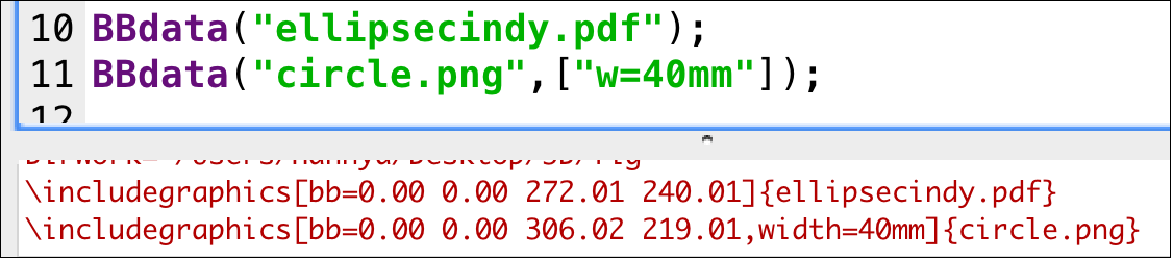
\includegraphics[bb=0.00 0.00 562.03 124.01,width=10cm]{Fig/bbdata.pdf} 


\vspace{\baselineskip}
\hypertarget{cindyname}{}
\item[関数]  Cindyname()
\item[機能]  作図中のファイル名を取得する。
\item[説明]  たとえば,現在作図しているファイル名が 「polygon.cdy」のとき,"polygon" を返す。
    
\vspace{\baselineskip}
\hypertarget{crossprod}{}
\item[関数]  Crossprod(リスト,リスト)
\item[機能]  2つのベクトルの外積を求める。
\item[説明]  Cindyscriptの組み込み関数 cross(リスト,リスト)と同じ。

\vspace{\baselineskip}
【例】\verb|Crossprod([1,0,0],[1,1,1]);|
  
      結果は  [0,-1,1]\\

\vspace{\baselineskip}
\hypertarget{dotprod}{}
\item[関数]  Dotprod(リスト,リスト)
\item[機能]  2つのベクトルの内積を求める。
\item[説明]  Cindyscriptでは,積の演算で内積が求められる。

\vspace{\baselineskip}
  【例】\verb|Dotprod([1,2,3],[1,-1,1]);|
  
      結果は  2
      
      [1,2,3]*[1,-1,1] でも同じ結果を得る。

\vspace{\baselineskip}
\hypertarget{findarea}{}
\item[関数]  Findarea(プロットデータ)
\item[機能]  プロットデータで囲まれる部分の面積を求める。
\item[説明]  閉曲線をなすプロットデータで囲まれる部分の面積を求める。大島のベジェ公式を用いている。

\vspace{\baselineskip}
【例】楕円の面積を求めて表示する。
\begin{verbatim}
    Paramplot("1","[3*cos(t),2*sin(t)]","t=[0,2*pi]");
    area=Findarea("gp1");
    println(Sprintf(area,6));
\end{verbatim}

コンソールに面積 18.849536 が表示される。 

\vspace{\baselineskip}
\hypertarget{findlength}{}
\item[関数]  Findlength(プロットデータ)
\item[機能]  プロットデータの曲線の長さを求める。
\item[説明]  プロットデータが描く曲線の長さを求める。大島のベジェ公式を用いている。

\vspace{\baselineskip}
【例】円周の長さを求めて表示する。
\begin{verbatim}
    Circledata("1",[[0,0],[2,0]]);
    len=Findlength("cr1");
    println(Sprintf(len,6)); 
\end{verbatim}

コンソールに 12.558097 が表示される。

\begin{flushright}  \hyperlink{functionlist}{$\Rightarrow$関数一覧}\end{flushright}

\end{description}
\newpage
%==============作表=====================
\subsection{作表}

\begin{description}

\hypertarget{tabledata}{}
\item[関数]  Tabledata(name , 縦横データ, 除外線 , options)
\item[機能]  表の枠を作成し,表のデータlist を返す
\item[説明]  Cinderellaの描画面上に左下を原点とする表を作成する。

他の関数との引数の整合性,\ketpic のコマンドとの整合性などから,先頭にnameの引数をつけるが,実際にはあまり利用しないので,空文字""でもよい。

除外線がない場合は空リストを指定する。(必須)

optionsは線種と"notex"など,および "Rng=n"。

"Rng=n" をつけると,NE,SWによる出力領域指定が有効になり,NE,SWをドラッグして出力領域を変更できる。(初期状態は,表の右上と左下)つけない場合は,表の部分だけが出力される。

縦横データには,次の2通りの書式がある。いずれも同じ表を作成する。

\vspace{\baselineskip}
(1) 横のセル数 , 縦のセル数 , 表の横幅 , 表の縦幅  を指定する。除外線なし。

\begin{verbatim}
    Tabledata("",4,5,80,50,[]);
\end{verbatim}
  
(2) 横と縦の幅を指定したリストを使う
\begin{verbatim}
    Yoko=[20,20,20,20];
    Tate=[10,10,10,10,10];
    Tabledata("",Yoko,Tate,[]);
 \end{verbatim}

幅はCinderellaの描画面の0.1を単位とする。

作成された表には,行,列の制御点がつく。画面上では,横罫線の番号 r0,r1,・・・  縦罫線の番号 c0,c1,・・・と見ることもできる。また,縦幅,横幅が数字で示される。ただし,これらは\TeX には出力されない。
また,作表はCinderellaの描画面上では座標平面上に置かれるが,\TeX への出力は座標平面上には置かないことが多いので,座標軸は非表示としている。

\hspace{25mm} 描画面 \hspace{45mm} TeX

\hspace{5mm}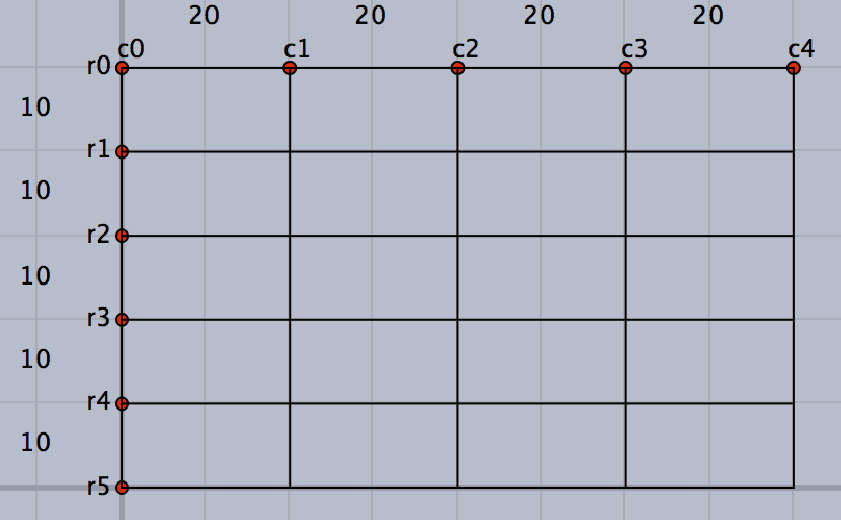
\includegraphics[bb=0 0 403.52 249.51 , width=5cm]{Fig/table01.pdf}   \hspace{10mm}  %%% test.tex 2014-11-24 21:36
%%% test.sce 2014-11-24 21:36
{\unitlength=6mm%
\begin{picture}%
(   8.00000,   5.00000)(   0.00000,   0.00000)%
\special{pn 8}%
%
\special{pa 0 -1181}\special{pa 472 -1181}%
\special{fp}%
\special{pa 472 -1181}\special{pa 945 -1181}%
\special{fp}%
\special{pa 945 -1181}\special{pa 1417 -1181}%
\special{fp}%
\special{pa 1417 -1181}\special{pa 1890 -1181}%
\special{fp}%
\special{pa 0 -945}\special{pa 472 -945}%
\special{fp}%
\special{pa 472 -945}\special{pa 945 -945}%
\special{fp}%
\special{pa 945 -945}\special{pa 1417 -945}%
\special{fp}%
\special{pa 1417 -945}\special{pa 1890 -945}%
\special{fp}%
\special{pa 0 -709}\special{pa 472 -709}%
\special{fp}%
\special{pa 472 -709}\special{pa 945 -709}%
\special{fp}%
\special{pa 945 -709}\special{pa 1417 -709}%
\special{fp}%
\special{pa 1417 -709}\special{pa 1890 -709}%
\special{fp}%
\special{pa 0 -472}\special{pa 472 -472}%
\special{fp}%
\special{pa 472 -472}\special{pa 945 -472}%
\special{fp}%
\special{pa 945 -472}\special{pa 1417 -472}%
\special{fp}%
\special{pa 1417 -472}\special{pa 1890 -472}%
\special{fp}%
\special{pa 0 -236}\special{pa 472 -236}%
\special{fp}%
\special{pa 472 -236}\special{pa 945 -236}%
\special{fp}%
\special{pa 945 -236}\special{pa 1417 -236}%
\special{fp}%
\special{pa 1417 -236}\special{pa 1890 -236}%
\special{fp}%
\special{pa 0 0}\special{pa 472 0}%
\special{fp}%
\special{pa 472 0}\special{pa 945 0}%
\special{fp}%
\special{pa 945 0}\special{pa 1417 0}%
\special{fp}%
\special{pa 1417 0}\special{pa 1890 0}%
\special{fp}%
\special{pa 0 -1181}\special{pa 0 -945}%
\special{fp}%
\special{pa 0 -945}\special{pa 0 -709}%
\special{fp}%
\special{pa 0 -709}\special{pa 0 -472}%
\special{fp}%
\special{pa 0 -472}\special{pa 0 -236}%
\special{fp}%
\special{pa 0 -236}\special{pa 0 0}%
\special{fp}%
\special{pa 472 -1181}\special{pa 472 -945}%
\special{fp}%
\special{pa 472 -945}\special{pa 472 -709}%
\special{fp}%
\special{pa 472 -709}\special{pa 472 -472}%
\special{fp}%
\special{pa 472 -472}\special{pa 472 -236}%
\special{fp}%
\special{pa 472 -236}\special{pa 472 0}%
\special{fp}%
\special{pa 945 -1181}\special{pa 945 -945}%
\special{fp}%
\special{pa 945 -945}\special{pa 945 -709}%
\special{fp}%
\special{pa 945 -709}\special{pa 945 -472}%
\special{fp}%
\special{pa 945 -472}\special{pa 945 -236}%
\special{fp}%
\special{pa 945 -236}\special{pa 945 0}%
\special{fp}%
\special{pa 1417 -1181}\special{pa 1417 -945}%
\special{fp}%
\special{pa 1417 -945}\special{pa 1417 -709}%
\special{fp}%
\special{pa 1417 -709}\special{pa 1417 -472}%
\special{fp}%
\special{pa 1417 -472}\special{pa 1417 -236}%
\special{fp}%
\special{pa 1417 -236}\special{pa 1417 0}%
\special{fp}%
\special{pa 1890 -1181}\special{pa 1890 -945}%
\special{fp}%
\special{pa 1890 -945}\special{pa 1890 -709}%
\special{fp}%
\special{pa 1890 -709}\special{pa 1890 -472}%
\special{fp}%
\special{pa 1890 -472}\special{pa 1890 -236}%
\special{fp}%
\special{pa 1890 -236}\special{pa 1890 0}%
\special{fp}%
\end{picture}}% 


  表のサイズ・行幅・列幅は,作成後にそれぞれの制御点をドラッグすることにより任意に変えることができる。

\vspace{\baselineskip}
除外線は,除外するセルの罫線を,rとc で位置指定する。
  
\hspace{10mm} 横罫線の場合,横罫線の番号,範囲(から,まで)

\hspace{10mm} 縦罫線の場合,縦罫線の番号,範囲(から,まで)

とする。

\vspace{\baselineskip}
【例】4つの罫線を非表示にする
\begin{verbatim}
    Rmv=["r1c0c1","c3r0r1","c3r3r5","r4c2c4"];
    Tabledata("",4,5,80,50,Rmv);
\end{verbatim}
      
で,次の表ができる。
  
\vspace{\baselineskip}
\hspace{20mm}  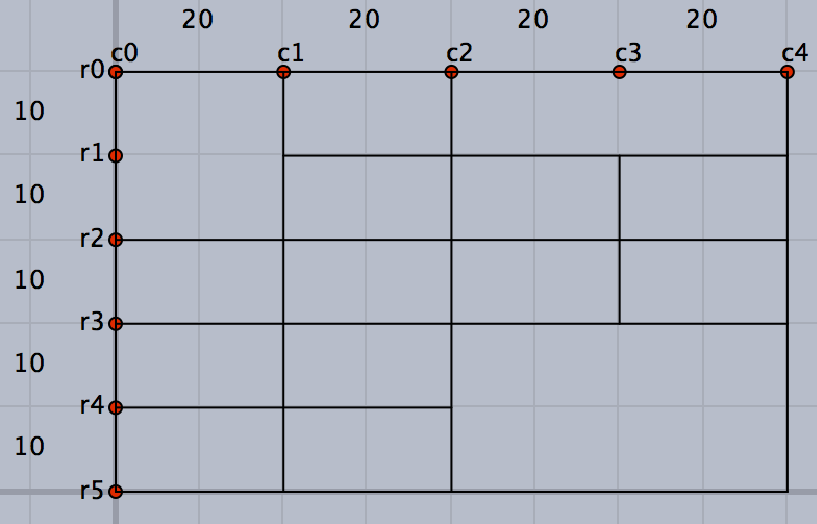
\includegraphics[bb=0 0 392.02 251.51 , width=6cm]{Fig/table03.pdf}

\vspace{\baselineskip}
<補足>

Tabledata()関数は,制御点r0,r1,・・・,c0,c1,・・・  がなければ新しく作り,すでに存在する場合はそのままとする。したがって,一度表を作成したのち,行数・列数を修正して作り直す場合は,一度既存の点を消去する必要がある。そのためには,「すべての点を選択する」ツールをクリックして点を消去するのがよい。クリックすると,消去後すぐに新規作成される。(誤って「すべての要素を選択する」を選ばないこと)
  
他の点が描画されている場合は,表の部分だけドラッグで選択するか,表示メニューの「式による表示」で一覧表を出して,制御点を選択して消去する。

\begin{flushright}  \hyperlink{functionlist}{$\Rightarrow$関数一覧}\end{flushright}

\vspace{\baselineskip}
\hypertarget{tabledatalight}{}
\item[関数]  Tabledatalight(name , 縦横データ, 除外線 , options)
\item[機能]  幾何点を持たない表の枠を作成し,表のデータlist を返す
\item[説明]  Tabledata()がCinderellaの幾何点を生成するのに対し,Tabledatalight()は幾何点を生成しない。

幾何点を作成しないメリットは,スクリプトだけで全体の縦横幅を変更できること。デメリットはインタラクティブな微調整ができないこと。
  
optionとして,ラベルのスキップ値(スキップするところは表示されない)を指定することができる。ただし,ラベルはCinderellaの画面上だけの問題。
  
\vspace{\baselineskip}
  【例】1つおきにスキップして,r1,r3,c1,c2 を非表示とする。
\begin{verbatim}
    Yoko=[20,20,20,20];
    Tate=[10,10,10,10,10];
    Tabledatalight("",Yoko,Tate,[],[2]);
\end{verbatim}
        
\vspace{\baselineskip}
\hypertarget{changetablestyle}{}
\item[関数]  ChangeTablestyle(罫線リスト, 変更オプション)
\item[機能]  Table の罫線の描画オプションを変更
\item[説明]  罫線の部分的に指定して描画オプションを変更できる。

\vspace{\baselineskip}
【例】

\verb|Tabledatalight("",[10,20,10,20],[10,10,10],[]);|\\
\verb|ChangeTablestyle(["r1c0c4"],["da"]);|\\
\verb|ChangeTablestyle(["r2c0c2","c1r0r3"],["nodisp"]);|

\vspace{\baselineskip}
\hspace{20mm}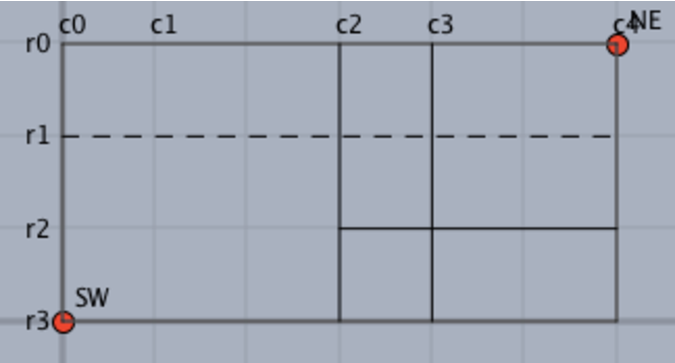
\includegraphics[bb=0.00 0.00 324.00 174.00,width=50mm]{Fig/changetable.pdf} 
    
\vspace{\baselineskip}
\hypertarget{findcell}{}
\item[関数]  Findcell(列番号, 行番号)
\item[機能]  セルの情報list(中心,横幅/2,縦幅/2)を返す
\item[説明]  列番号,行番号は左上のセルを1列1行として数える。

\vspace{\baselineskip}
【例】\verb|Tabledata(4,5,80,50,[]);|

    \verb|println(Findcell(tb,2,1));|
    
    とすると,2列1行のセルの中心の座標と横幅の半分,縦幅の半分の値がリストとしてコンソールに表示される。結果は [[3,4.5],1,0.5]

\vspace{\baselineskip}
\hypertarget{putcell}{}
\item[関数]  Putcell (列番号, 行番号, 位置, 文字データ)
\item[機能]  セルに文字列を入れる
\item[説明]  複数のセルにまたぐ位置指定の場合,列番号,行番号は,セル左上と右下の制御点の名称で指定する。

位置は  c, r, l, t, b (中央center , 右right , 左left , 上top , 下bottom   )
  
位置の例を以下に示す。
\begin{verbatim}
    Tabledata("",5,2,100,40,["c1r1r2","c4r1r2"]);
    Putcell(1,1,"c","A");
    Putcell(2,1,"r","B");
    Putcell(3,1,"l","C");
    Putcell(4,1,"t","D");
    Putcell(5,1,"b","E");
    Putcell("c0r1","c2r2","c","F");
    Putcell("c2r1","c3r2","lb","G");
    Putcell("c3r1","c5r2","rt","H");
\end{verbatim}
\vspace{\baselineskip}
      \begin{center} %%% /Users/Hannya/Desktop/KeTCindy/fig/putcell.tex 
%%% Generator=template1basic.cdy 
{\unitlength=7mm%
\begin{picture}%
(10,4)(0,0)%
\special{pn 8}%
%
\special{pa     0 -1102}\special{pa     0    -0}%
\special{fp}%
\special{pa  1102 -1102}\special{pa  1102    -0}%
\special{fp}%
\special{pa  1654 -1102}\special{pa  1654    -0}%
\special{fp}%
\special{pa  2756 -1102}\special{pa  2756    -0}%
\special{fp}%
\special{pa     0 -1102}\special{pa  2756 -1102}%
\special{fp}%
\special{pa     0  -551}\special{pa  2756  -551}%
\special{fp}%
\special{pa     0    -0}\special{pa  2756    -0}%
\special{fp}%
\special{pa   551 -1102}\special{pa   551  -551}%
\special{fp}%
\special{pa  2205 -1102}\special{pa  2205  -551}%
\special{fp}%
\settowidth{\Width}{A}\setlength{\Width}{-0.5\Width}%
\settoheight{\Height}{A}\settodepth{\Depth}{A}\setlength{\Height}{-0.5\Height}\setlength{\Depth}{0.5\Depth}\addtolength{\Height}{\Depth}%
\put(1.0000000,3.0000000){\hspace*{\Width}\raisebox{\Height}{A}}%
%
\settowidth{\Width}{B}\setlength{\Width}{-1\Width}%
\settoheight{\Height}{B}\settodepth{\Depth}{B}\setlength{\Height}{-0.5\Height}\setlength{\Depth}{0.5\Depth}\addtolength{\Height}{\Depth}%
\put(3.9285714,3.0000000){\hspace*{\Width}\raisebox{\Height}{B}}%
%
\settowidth{\Width}{C}\setlength{\Width}{0\Width}%
\settoheight{\Height}{C}\settodepth{\Depth}{C}\setlength{\Height}{-0.5\Height}\setlength{\Depth}{0.5\Depth}\addtolength{\Height}{\Depth}%
\put(4.0714286,3.0000000){\hspace*{\Width}\raisebox{\Height}{C}}%
%
\settowidth{\Width}{D}\setlength{\Width}{-0.5\Width}%
\settoheight{\Height}{D}\settodepth{\Depth}{D}\setlength{\Height}{-\Height}%
\put(7.0000000,3.9285714){\hspace*{\Width}\raisebox{\Height}{D}}%
%
\settowidth{\Width}{E}\setlength{\Width}{-0.5\Width}%
\settoheight{\Height}{E}\settodepth{\Depth}{E}\setlength{\Height}{\Depth}%
\put(9.0000000,2.0714286){\hspace*{\Width}\raisebox{\Height}{E}}%
%
\settowidth{\Width}{F}\setlength{\Width}{-0.5\Width}%
\settoheight{\Height}{F}\settodepth{\Depth}{F}\setlength{\Height}{-0.5\Height}\setlength{\Depth}{0.5\Depth}\addtolength{\Height}{\Depth}%
\put(2.0000000,1.0000000){\hspace*{\Width}\raisebox{\Height}{F}}%
%
\settowidth{\Width}{G}\setlength{\Width}{0\Width}%
\settoheight{\Height}{G}\settodepth{\Depth}{G}\setlength{\Height}{\Depth}%
\put(4.0714286,0.0714286){\hspace*{\Width}\raisebox{\Height}{G}}%
%
\settowidth{\Width}{H}\setlength{\Width}{-1\Width}%
\settoheight{\Height}{H}\settodepth{\Depth}{H}\setlength{\Height}{-\Height}%
\put(9.9285714,1.9285714){\hspace*{\Width}\raisebox{\Height}{H}}%
%
\settowidth{\Width}{c0}\setlength{\Width}{0\Width}%
\settoheight{\Height}{c0}\settodepth{\Depth}{c0}\setlength{\Height}{\Depth}%
\put(0.0714286,4.2142857){\hspace*{\Width}\raisebox{\Height}{c0}}%
%
\settowidth{\Width}{c1}\setlength{\Width}{0\Width}%
\settoheight{\Height}{c1}\settodepth{\Depth}{c1}\setlength{\Height}{\Depth}%
\put(2.0714286,4.2142857){\hspace*{\Width}\raisebox{\Height}{c1}}%
%
\settowidth{\Width}{c2}\setlength{\Width}{0\Width}%
\settoheight{\Height}{c2}\settodepth{\Depth}{c2}\setlength{\Height}{\Depth}%
\put(4.0714286,4.2142857){\hspace*{\Width}\raisebox{\Height}{c2}}%
%
\settowidth{\Width}{c3}\setlength{\Width}{0\Width}%
\settoheight{\Height}{c3}\settodepth{\Depth}{c3}\setlength{\Height}{\Depth}%
\put(6.0714286,4.2142857){\hspace*{\Width}\raisebox{\Height}{c3}}%
%
\settowidth{\Width}{c4}\setlength{\Width}{0\Width}%
\settoheight{\Height}{c4}\settodepth{\Depth}{c4}\setlength{\Height}{\Depth}%
\put(8.0714286,4.2142857){\hspace*{\Width}\raisebox{\Height}{c4}}%
%
\settowidth{\Width}{c5}\setlength{\Width}{0\Width}%
\settoheight{\Height}{c5}\settodepth{\Depth}{c5}\setlength{\Height}{\Depth}%
\put(10.0714286,4.2142857){\hspace*{\Width}\raisebox{\Height}{c5}}%
%
\settowidth{\Width}{r2}\setlength{\Width}{-1\Width}%
\settoheight{\Height}{r2}\settodepth{\Depth}{r2}\setlength{\Height}{-0.5\Height}\setlength{\Depth}{0.5\Depth}\addtolength{\Height}{\Depth}%
\put(-0.0714286,0.0000000){\hspace*{\Width}\raisebox{\Height}{r2}}%
%
\settowidth{\Width}{r1}\setlength{\Width}{-1\Width}%
\settoheight{\Height}{r1}\settodepth{\Depth}{r1}\setlength{\Height}{-0.5\Height}\setlength{\Depth}{0.5\Depth}\addtolength{\Height}{\Depth}%
\put(-0.0714286,2.0000000){\hspace*{\Width}\raisebox{\Height}{r1}}%
%
\settowidth{\Width}{r0}\setlength{\Width}{-1\Width}%
\settoheight{\Height}{r0}\settodepth{\Depth}{r0}\setlength{\Height}{-0.5\Height}\setlength{\Depth}{0.5\Depth}\addtolength{\Height}{\Depth}%
\put(-0.0714286,4.0000000){\hspace*{\Width}\raisebox{\Height}{r0}}%
%
\end{picture}}% \end{center}

  ※r0,c0,・・は画面に表示される番号

\begin{flushright}  \hyperlink{functionlist}{$\Rightarrow$関数一覧}\end{flushright}

\vspace{\baselineskip}
\hypertarget{putcol}{}
\item[関数]  PutcoL (列番号, 文字位置,文字列リスト)
\item[機能]  1列に順に文字を書き入れる
\item[説明]  列番号で指定した列に,第1行から順に文字列リストの文字を書き入れる\\
  数の場合はダブルクウォートでくくらなくてもよい。
  
  セルを飛ばす場合は,ヌル文字列 "" を書く。
  
\vspace{\baselineskip}
\hypertarget{putcolexpr}{}
\item[関数]  PutcoLexpr (列番号, 文字位置,文字列リスト)
\item[機能]  1列に順に文字を書き入れる
\item[説明]  文字列に\TeX 書式を使うことができる

\vspace{\baselineskip}
\hypertarget{putrow}{}
\item[関数]  Putrow (行番号, 文字位置,文字列リスト)
\item[機能]  1行に順に文字を書き入れる
\item[説明]  行番号で指定した行に,第1列から順に文字列リストの文字を書き入れる。


\vspace{\baselineskip}
\hypertarget{putrowexpr}{}
\item[関数]  Putrowexpr (行番号, 文字位置,文字列リスト)
\item[機能]  1行に順に文字を書き入れる
\item[説明]  文字列に\TeX 書式を使うことができる

文字を入れる例を示す。
\begin{verbatim}
    Tabledata("",5,3,100,45,["c1r1r2","r1c2c3","r2c2c3"]);
    PutcoL(3,"c",["A","B","C"]);
    PutcoLexpr(4,"l",["x^2","y=\sqrt{x^3}"]);
    Putrow(1,"c",[1,"二"]);
    Putrowexpr(3,"c",["","\frac{\pi}{2}","","","\sum{x^2}"]);
\end{verbatim}
 \vspace{\baselineskip}
          \begin{center} %%% /Users/Hannya/Desktop/KeTCindy/fig/putcol.tex 
%%% Generator=template1basic.cdy 
{\unitlength=7mm%
\begin{picture}%
(10,4.5)(0,0)%
\special{pn 8}%
%
\special{pa     0 -1240}\special{pa     0    -0}%
\special{fp}%
\special{pa  1102 -1240}\special{pa  1102    -0}%
\special{fp}%
\special{pa  1654 -1240}\special{pa  1654    -0}%
\special{fp}%
\special{pa  2205 -1240}\special{pa  2205    -0}%
\special{fp}%
\special{pa  2756 -1240}\special{pa  2756    -0}%
\special{fp}%
\special{pa     0 -1240}\special{pa  2756 -1240}%
\special{fp}%
\special{pa     0    -0}\special{pa  2756    -0}%
\special{fp}%
\special{pa   551 -1240}\special{pa   551  -827}%
\special{fp}%
\special{pa   551  -413}\special{pa   551    -0}%
\special{fp}%
\special{pa     0  -827}\special{pa  1102  -827}%
\special{fp}%
\special{pa  1654  -827}\special{pa  2756  -827}%
\special{fp}%
\special{pa     0  -413}\special{pa  1102  -413}%
\special{fp}%
\special{pa  1654  -413}\special{pa  2756  -413}%
\special{fp}%
\settowidth{\Width}{A}\setlength{\Width}{-0.5\Width}%
\settoheight{\Height}{A}\settodepth{\Depth}{A}\setlength{\Height}{-0.5\Height}\setlength{\Depth}{0.5\Depth}\addtolength{\Height}{\Depth}%
\put(5.0000000,3.7500000){\hspace*{\Width}\raisebox{\Height}{A}}%
%
\settowidth{\Width}{B}\setlength{\Width}{-0.5\Width}%
\settoheight{\Height}{B}\settodepth{\Depth}{B}\setlength{\Height}{-0.5\Height}\setlength{\Depth}{0.5\Depth}\addtolength{\Height}{\Depth}%
\put(5.0000000,2.2500000){\hspace*{\Width}\raisebox{\Height}{B}}%
%
\settowidth{\Width}{C}\setlength{\Width}{-0.5\Width}%
\settoheight{\Height}{C}\settodepth{\Depth}{C}\setlength{\Height}{-0.5\Height}\setlength{\Depth}{0.5\Depth}\addtolength{\Height}{\Depth}%
\put(5.0000000,0.7500000){\hspace*{\Width}\raisebox{\Height}{C}}%
%
\settowidth{\Width}{$x^2$}\setlength{\Width}{0\Width}%
\settoheight{\Height}{$x^2$}\settodepth{\Depth}{$x^2$}\setlength{\Height}{-0.5\Height}\setlength{\Depth}{0.5\Depth}\addtolength{\Height}{\Depth}%
\put(6.0714286,3.7500000){\hspace*{\Width}\raisebox{\Height}{$x^2$}}%
%
\settowidth{\Width}{$y=\sqrt{x^3}$}\setlength{\Width}{0\Width}%
\settoheight{\Height}{$y=\sqrt{x^3}$}\settodepth{\Depth}{$y=\sqrt{x^3}$}\setlength{\Height}{-0.5\Height}\setlength{\Depth}{0.5\Depth}\addtolength{\Height}{\Depth}%
\put(6.0714286,2.2500000){\hspace*{\Width}\raisebox{\Height}{$y=\sqrt{x^3}$}}%
%
\settowidth{\Width}{1}\setlength{\Width}{-0.5\Width}%
\settoheight{\Height}{1}\settodepth{\Depth}{1}\setlength{\Height}{-0.5\Height}\setlength{\Depth}{0.5\Depth}\addtolength{\Height}{\Depth}%
\put(1.0000000,3.7500000){\hspace*{\Width}\raisebox{\Height}{1}}%
%
\settowidth{\Width}{二}\setlength{\Width}{-0.5\Width}%
\settoheight{\Height}{二}\settodepth{\Depth}{二}\setlength{\Height}{-0.5\Height}\setlength{\Depth}{0.5\Depth}\addtolength{\Height}{\Depth}%
\put(3.0000000,3.7500000){\hspace*{\Width}\raisebox{\Height}{二}}%
%
\settowidth{\Width}{$$}\setlength{\Width}{-0.5\Width}%
\settoheight{\Height}{$$}\settodepth{\Depth}{$$}\setlength{\Height}{-0.5\Height}\setlength{\Depth}{0.5\Depth}\addtolength{\Height}{\Depth}%
\put(1.0000000,0.7500000){\hspace*{\Width}\raisebox{\Height}{$$}}%
%
\settowidth{\Width}{$\frac{\pi}{2}$}\setlength{\Width}{-0.5\Width}%
\settoheight{\Height}{$\frac{\pi}{2}$}\settodepth{\Depth}{$\frac{\pi}{2}$}\setlength{\Height}{-0.5\Height}\setlength{\Depth}{0.5\Depth}\addtolength{\Height}{\Depth}%
\put(3.0000000,0.7500000){\hspace*{\Width}\raisebox{\Height}{$\frac{\pi}{2}$}}%
%
\settowidth{\Width}{$$}\setlength{\Width}{-0.5\Width}%
\settoheight{\Height}{$$}\settodepth{\Depth}{$$}\setlength{\Height}{-0.5\Height}\setlength{\Depth}{0.5\Depth}\addtolength{\Height}{\Depth}%
\put(5.0000000,0.7500000){\hspace*{\Width}\raisebox{\Height}{$$}}%
%
\settowidth{\Width}{$$}\setlength{\Width}{-0.5\Width}%
\settoheight{\Height}{$$}\settodepth{\Depth}{$$}\setlength{\Height}{-0.5\Height}\setlength{\Depth}{0.5\Depth}\addtolength{\Height}{\Depth}%
\put(7.0000000,0.7500000){\hspace*{\Width}\raisebox{\Height}{$$}}%
%
\settowidth{\Width}{$\sum{x^2}$}\setlength{\Width}{-0.5\Width}%
\settoheight{\Height}{$\sum{x^2}$}\settodepth{\Depth}{$\sum{x^2}$}\setlength{\Height}{-0.5\Height}\setlength{\Depth}{0.5\Depth}\addtolength{\Height}{\Depth}%
\put(9.0000000,0.7500000){\hspace*{\Width}\raisebox{\Height}{$\sum{x^2}$}}%
%
\settowidth{\Width}{c0}\setlength{\Width}{0\Width}%
\settoheight{\Height}{c0}\settodepth{\Depth}{c0}\setlength{\Height}{\Depth}%
\put(0.0714286,4.7142857){\hspace*{\Width}\raisebox{\Height}{c0}}%
%
\settowidth{\Width}{c1}\setlength{\Width}{0\Width}%
\settoheight{\Height}{c1}\settodepth{\Depth}{c1}\setlength{\Height}{\Depth}%
\put(2.0714286,4.7142857){\hspace*{\Width}\raisebox{\Height}{c1}}%
%
\settowidth{\Width}{c2}\setlength{\Width}{0\Width}%
\settoheight{\Height}{c2}\settodepth{\Depth}{c2}\setlength{\Height}{\Depth}%
\put(4.0714286,4.7142857){\hspace*{\Width}\raisebox{\Height}{c2}}%
%
\settowidth{\Width}{c3}\setlength{\Width}{0\Width}%
\settoheight{\Height}{c3}\settodepth{\Depth}{c3}\setlength{\Height}{\Depth}%
\put(6.0714286,4.7142857){\hspace*{\Width}\raisebox{\Height}{c3}}%
%
\settowidth{\Width}{c4}\setlength{\Width}{0\Width}%
\settoheight{\Height}{c4}\settodepth{\Depth}{c4}\setlength{\Height}{\Depth}%
\put(8.0714286,4.7142857){\hspace*{\Width}\raisebox{\Height}{c4}}%
%
\settowidth{\Width}{c5}\setlength{\Width}{0\Width}%
\settoheight{\Height}{c5}\settodepth{\Depth}{c5}\setlength{\Height}{\Depth}%
\put(10.0714286,4.7142857){\hspace*{\Width}\raisebox{\Height}{c5}}%
%
\settowidth{\Width}{r3}\setlength{\Width}{-1\Width}%
\settoheight{\Height}{r3}\settodepth{\Depth}{r3}\setlength{\Height}{-0.5\Height}\setlength{\Depth}{0.5\Depth}\addtolength{\Height}{\Depth}%
\put(-0.0714286,0.0000000){\hspace*{\Width}\raisebox{\Height}{r3}}%
%
\settowidth{\Width}{r2}\setlength{\Width}{-1\Width}%
\settoheight{\Height}{r2}\settodepth{\Depth}{r2}\setlength{\Height}{-0.5\Height}\setlength{\Depth}{0.5\Depth}\addtolength{\Height}{\Depth}%
\put(-0.0714286,1.5000000){\hspace*{\Width}\raisebox{\Height}{r2}}%
%
\settowidth{\Width}{r1}\setlength{\Width}{-1\Width}%
\settoheight{\Height}{r1}\settodepth{\Depth}{r1}\setlength{\Height}{-0.5\Height}\setlength{\Depth}{0.5\Depth}\addtolength{\Height}{\Depth}%
\put(-0.0714286,3.0000000){\hspace*{\Width}\raisebox{\Height}{r1}}%
%
\settowidth{\Width}{r0}\setlength{\Width}{-1\Width}%
\settoheight{\Height}{r0}\settodepth{\Depth}{r0}\setlength{\Height}{-0.5\Height}\setlength{\Depth}{0.5\Depth}\addtolength{\Height}{\Depth}%
\put(-0.0714286,4.5000000){\hspace*{\Width}\raisebox{\Height}{r0}}%
%
\end{picture}}% \end{center}

  ※ r0,c0,・・は画面に表示される番号。

グラフや文を入れた表の作成例

  PutcoLexpr(),Putrowexpr() では,数式だけでなく,一般の\TeX の文を入れることができる。
  また,グラフの位置を適当に合わせて描画することにより,表のセルの中にグラフを入れることができる。

\vspace{\baselineskip}
  【例】2次関数のグラフと2次方程式の判別式の関係
  
セルの中にグラフを描く例。実際には,セルの位置にグラフを描く。

x軸を描くための点A〜Fは作図ツールでとっておく。

スクリプトを実行して表ができたら,制御点をドラッグしてサイズを調整し,点A〜Fもドラッグして軸と放物線の共有状況を示すようにする。

\vspace{\baselineskip}
\begin{verbatim}
    Tabledata("",3,3,120,60,[],["dr,2"]);
    ChangeTablestyle(["r1c0c3"],["dr"]);
    ChangeTablestyle(["r2c0c3"],["da"]);
    Plotdata("1","(x-2)^2+0.5","x=[0.5,3.5]");
    Plotdata("2","(x-6)^2+1","x=[4.5,7.5]");
    Plotdata("3","(x-10)^2+1.5","x=[8.5,11.5]");
    Listplot([A,B]);
    Listplot([C,D]);
    Listplot([E,F]);
    Putrowexpr(1,"c",["D>0","D=0","D<0"]);
    Putrow(2,"c",["2点で交わる","接する","共有点なし"]);
\end{verbatim}

\vspace{\baselineskip}
 \begin{center}\scalebox{0.9}{ %%% /Users/takatoosetsuo/Dropbox/kettoday/0511ReuleauxTriangle/fig/tablesample1.tex 
%%% Generator=tablesample1.cdy 
{\unitlength=1cm%
\begin{picture}%
(12,6)(0,0)%
\special{pn 8}%
%
\special{pn 16}%
\special{pa     0 -2362}\special{pa     0    -0}%
\special{fp}%
\special{pn 8}%
\special{pn 16}%
\special{pa  1575 -2362}\special{pa  1575    -0}%
\special{fp}%
\special{pn 8}%
\special{pn 16}%
\special{pa  3150 -2362}\special{pa  3150    -0}%
\special{fp}%
\special{pn 8}%
\special{pn 16}%
\special{pa  4724 -2362}\special{pa  4724    -0}%
\special{fp}%
\special{pn 8}%
\special{pn 16}%
\special{pa     0 -2362}\special{pa  4724 -2362}%
\special{fp}%
\special{pn 8}%
\special{pn 16}%
\special{pa     0    -0}\special{pa  4724    -0}%
\special{fp}%
\special{pn 8}%
\special{pa     0 -1969}\special{pa  4724 -1969}%
\special{fp}%
\special{pa     0 -1969}\special{pa  4724 -1969}%
\special{fp}%
\special{pa 0 -1575}\special{pa 39 -1575}\special{fp}\special{pa 78 -1575}\special{pa 117 -1575}\special{fp}%
\special{pa 156 -1575}\special{pa 195 -1575}\special{fp}\special{pa 234 -1575}\special{pa 273 -1575}\special{fp}%
\special{pa 312 -1575}\special{pa 351 -1575}\special{fp}\special{pa 390 -1575}\special{pa 429 -1575}\special{fp}%
\special{pa 469 -1575}\special{pa 508 -1575}\special{fp}\special{pa 547 -1575}\special{pa 586 -1575}\special{fp}%
\special{pa 625 -1575}\special{pa 664 -1575}\special{fp}\special{pa 703 -1575}\special{pa 742 -1575}\special{fp}%
\special{pa 781 -1575}\special{pa 820 -1575}\special{fp}\special{pa 859 -1575}\special{pa 898 -1575}\special{fp}%
\special{pa 937 -1575}\special{pa 976 -1575}\special{fp}\special{pa 1015 -1575}\special{pa 1054 -1575}\special{fp}%
\special{pa 1093 -1575}\special{pa 1132 -1575}\special{fp}\special{pa 1171 -1575}\special{pa 1210 -1575}\special{fp}%
\special{pa 1249 -1575}\special{pa 1288 -1575}\special{fp}\special{pa 1328 -1575}\special{pa 1367 -1575}\special{fp}%
\special{pa 1406 -1575}\special{pa 1445 -1575}\special{fp}\special{pa 1484 -1575}\special{pa 1523 -1575}\special{fp}%
\special{pa 1562 -1575}\special{pa 1601 -1575}\special{fp}\special{pa 1640 -1575}\special{pa 1679 -1575}\special{fp}%
\special{pa 1718 -1575}\special{pa 1757 -1575}\special{fp}\special{pa 1796 -1575}\special{pa 1835 -1575}\special{fp}%
\special{pa 1874 -1575}\special{pa 1913 -1575}\special{fp}\special{pa 1952 -1575}\special{pa 1991 -1575}\special{fp}%
\special{pa 2030 -1575}\special{pa 2069 -1575}\special{fp}\special{pa 2108 -1575}\special{pa 2147 -1575}\special{fp}%
\special{pa 2187 -1575}\special{pa 2226 -1575}\special{fp}\special{pa 2265 -1575}\special{pa 2304 -1575}\special{fp}%
\special{pa 2343 -1575}\special{pa 2382 -1575}\special{fp}\special{pa 2421 -1575}\special{pa 2460 -1575}\special{fp}%
\special{pa 2499 -1575}\special{pa 2538 -1575}\special{fp}\special{pa 2577 -1575}\special{pa 2616 -1575}\special{fp}%
\special{pa 2655 -1575}\special{pa 2694 -1575}\special{fp}\special{pa 2733 -1575}\special{pa 2772 -1575}\special{fp}%
\special{pa 2811 -1575}\special{pa 2850 -1575}\special{fp}\special{pa 2889 -1575}\special{pa 2928 -1575}\special{fp}%
\special{pa 2967 -1575}\special{pa 3006 -1575}\special{fp}\special{pa 3045 -1575}\special{pa 3085 -1575}\special{fp}%
\special{pa 3124 -1575}\special{pa 3163 -1575}\special{fp}\special{pa 3202 -1575}\special{pa 3241 -1575}\special{fp}%
\special{pa 3280 -1575}\special{pa 3319 -1575}\special{fp}\special{pa 3358 -1575}\special{pa 3397 -1575}\special{fp}%
\special{pa 3436 -1575}\special{pa 3475 -1575}\special{fp}\special{pa 3514 -1575}\special{pa 3553 -1575}\special{fp}%
\special{pa 3592 -1575}\special{pa 3631 -1575}\special{fp}\special{pa 3670 -1575}\special{pa 3709 -1575}\special{fp}%
\special{pa 3748 -1575}\special{pa 3787 -1575}\special{fp}\special{pa 3826 -1575}\special{pa 3865 -1575}\special{fp}%
\special{pa 3904 -1575}\special{pa 3944 -1575}\special{fp}\special{pa 3983 -1575}\special{pa 4022 -1575}\special{fp}%
\special{pa 4061 -1575}\special{pa 4100 -1575}\special{fp}\special{pa 4139 -1575}\special{pa 4178 -1575}\special{fp}%
\special{pa 4217 -1575}\special{pa 4256 -1575}\special{fp}\special{pa 4295 -1575}\special{pa 4334 -1575}\special{fp}%
\special{pa 4373 -1575}\special{pa 4412 -1575}\special{fp}\special{pa 4451 -1575}\special{pa 4490 -1575}\special{fp}%
\special{pa 4529 -1575}\special{pa 4568 -1575}\special{fp}\special{pa 4607 -1575}\special{pa 4646 -1575}\special{fp}%
\special{pa 4685 -1575}\special{pa 4724 -1575}\special{fp}%
%
\special{pa 0 -1575}\special{pa 39 -1575}\special{fp}\special{pa 78 -1575}\special{pa 117 -1575}\special{fp}%
\special{pa 156 -1575}\special{pa 195 -1575}\special{fp}\special{pa 234 -1575}\special{pa 273 -1575}\special{fp}%
\special{pa 312 -1575}\special{pa 351 -1575}\special{fp}\special{pa 390 -1575}\special{pa 429 -1575}\special{fp}%
\special{pa 469 -1575}\special{pa 508 -1575}\special{fp}\special{pa 547 -1575}\special{pa 586 -1575}\special{fp}%
\special{pa 625 -1575}\special{pa 664 -1575}\special{fp}\special{pa 703 -1575}\special{pa 742 -1575}\special{fp}%
\special{pa 781 -1575}\special{pa 820 -1575}\special{fp}\special{pa 859 -1575}\special{pa 898 -1575}\special{fp}%
\special{pa 937 -1575}\special{pa 976 -1575}\special{fp}\special{pa 1015 -1575}\special{pa 1054 -1575}\special{fp}%
\special{pa 1093 -1575}\special{pa 1132 -1575}\special{fp}\special{pa 1171 -1575}\special{pa 1210 -1575}\special{fp}%
\special{pa 1249 -1575}\special{pa 1288 -1575}\special{fp}\special{pa 1328 -1575}\special{pa 1367 -1575}\special{fp}%
\special{pa 1406 -1575}\special{pa 1445 -1575}\special{fp}\special{pa 1484 -1575}\special{pa 1523 -1575}\special{fp}%
\special{pa 1562 -1575}\special{pa 1601 -1575}\special{fp}\special{pa 1640 -1575}\special{pa 1679 -1575}\special{fp}%
\special{pa 1718 -1575}\special{pa 1757 -1575}\special{fp}\special{pa 1796 -1575}\special{pa 1835 -1575}\special{fp}%
\special{pa 1874 -1575}\special{pa 1913 -1575}\special{fp}\special{pa 1952 -1575}\special{pa 1991 -1575}\special{fp}%
\special{pa 2030 -1575}\special{pa 2069 -1575}\special{fp}\special{pa 2108 -1575}\special{pa 2147 -1575}\special{fp}%
\special{pa 2187 -1575}\special{pa 2226 -1575}\special{fp}\special{pa 2265 -1575}\special{pa 2304 -1575}\special{fp}%
\special{pa 2343 -1575}\special{pa 2382 -1575}\special{fp}\special{pa 2421 -1575}\special{pa 2460 -1575}\special{fp}%
\special{pa 2499 -1575}\special{pa 2538 -1575}\special{fp}\special{pa 2577 -1575}\special{pa 2616 -1575}\special{fp}%
\special{pa 2655 -1575}\special{pa 2694 -1575}\special{fp}\special{pa 2733 -1575}\special{pa 2772 -1575}\special{fp}%
\special{pa 2811 -1575}\special{pa 2850 -1575}\special{fp}\special{pa 2889 -1575}\special{pa 2928 -1575}\special{fp}%
\special{pa 2967 -1575}\special{pa 3006 -1575}\special{fp}\special{pa 3045 -1575}\special{pa 3085 -1575}\special{fp}%
\special{pa 3124 -1575}\special{pa 3163 -1575}\special{fp}\special{pa 3202 -1575}\special{pa 3241 -1575}\special{fp}%
\special{pa 3280 -1575}\special{pa 3319 -1575}\special{fp}\special{pa 3358 -1575}\special{pa 3397 -1575}\special{fp}%
\special{pa 3436 -1575}\special{pa 3475 -1575}\special{fp}\special{pa 3514 -1575}\special{pa 3553 -1575}\special{fp}%
\special{pa 3592 -1575}\special{pa 3631 -1575}\special{fp}\special{pa 3670 -1575}\special{pa 3709 -1575}\special{fp}%
\special{pa 3748 -1575}\special{pa 3787 -1575}\special{fp}\special{pa 3826 -1575}\special{pa 3865 -1575}\special{fp}%
\special{pa 3904 -1575}\special{pa 3944 -1575}\special{fp}\special{pa 3983 -1575}\special{pa 4022 -1575}\special{fp}%
\special{pa 4061 -1575}\special{pa 4100 -1575}\special{fp}\special{pa 4139 -1575}\special{pa 4178 -1575}\special{fp}%
\special{pa 4217 -1575}\special{pa 4256 -1575}\special{fp}\special{pa 4295 -1575}\special{pa 4334 -1575}\special{fp}%
\special{pa 4373 -1575}\special{pa 4412 -1575}\special{fp}\special{pa 4451 -1575}\special{pa 4490 -1575}\special{fp}%
\special{pa 4529 -1575}\special{pa 4568 -1575}\special{fp}\special{pa 4607 -1575}\special{pa 4646 -1575}\special{fp}%
\special{pa 4685 -1575}\special{pa 4724 -1575}\special{fp}%
%
\special{pa   197 -1083}\special{pa   220 -1013}\special{pa   244  -947}\special{pa   268  -883}%
\special{pa   291  -822}\special{pa   315  -764}\special{pa   339  -709}\special{pa   362  -656}%
\special{pa   386  -606}\special{pa   409  -560}\special{pa   433  -516}\special{pa   457  -475}%
\special{pa   480  -436}\special{pa   504  -401}\special{pa   528  -368}\special{pa   551  -339}%
\special{pa   575  -312}\special{pa   598  -288}\special{pa   622  -266}\special{pa   646  -248}%
\special{pa   669  -232}\special{pa   693  -220}\special{pa   717  -210}\special{pa   740  -203}%
\special{pa   764  -198}\special{pa   787  -197}\special{pa   811  -198}\special{pa   835  -203}%
\special{pa   858  -210}\special{pa   882  -220}\special{pa   906  -232}\special{pa   929  -248}%
\special{pa   953  -266}\special{pa   976  -288}\special{pa  1000  -312}\special{pa  1024  -339}%
\special{pa  1047  -368}\special{pa  1071  -401}\special{pa  1094  -436}\special{pa  1118  -475}%
\special{pa  1142  -516}\special{pa  1165  -560}\special{pa  1189  -606}\special{pa  1213  -656}%
\special{pa  1236  -709}\special{pa  1260  -764}\special{pa  1283  -822}\special{pa  1307  -883}%
\special{pa  1331  -947}\special{pa  1354 -1013}\special{pa  1378 -1083}%
\special{fp}%
\special{pa   197  -394}\special{pa  1378  -394}%
\special{fp}%
\special{pa  1772 -1280}\special{pa  1795 -1210}\special{pa  1819 -1143}\special{pa  1843 -1080}%
\special{pa  1866 -1019}\special{pa  1890  -961}\special{pa  1913  -905}\special{pa  1937  -853}%
\special{pa  1961  -803}\special{pa  1984  -757}\special{pa  2008  -713}\special{pa  2031  -671}%
\special{pa  2055  -633}\special{pa  2079  -598}\special{pa  2102  -565}\special{pa  2126  -535}%
\special{pa  2150  -509}\special{pa  2173  -484}\special{pa  2197  -463}\special{pa  2220  -445}%
\special{pa  2244  -429}\special{pa  2268  -416}\special{pa  2291  -406}\special{pa  2315  -399}%
\special{pa  2339  -395}\special{pa  2362  -394}\special{pa  2386  -395}\special{pa  2409  -399}%
\special{pa  2433  -406}\special{pa  2457  -416}\special{pa  2480  -429}\special{pa  2504  -445}%
\special{pa  2528  -463}\special{pa  2551  -484}\special{pa  2575  -509}\special{pa  2598  -535}%
\special{pa  2622  -565}\special{pa  2646  -598}\special{pa  2669  -633}\special{pa  2693  -671}%
\special{pa  2717  -713}\special{pa  2740  -757}\special{pa  2764  -803}\special{pa  2787  -853}%
\special{pa  2811  -905}\special{pa  2835  -961}\special{pa  2858 -1019}\special{pa  2882 -1080}%
\special{pa  2906 -1143}\special{pa  2929 -1210}\special{pa  2953 -1280}%
\special{fp}%
\special{pa  1772  -394}\special{pa  2953  -394}%
\special{fp}%
\special{pa  3346 -1476}\special{pa  3370 -1407}\special{pa  3394 -1340}\special{pa  3417 -1277}%
\special{pa  3441 -1216}\special{pa  3465 -1157}\special{pa  3488 -1102}\special{pa  3512 -1050}%
\special{pa  3535 -1000}\special{pa  3559  -953}\special{pa  3583  -909}\special{pa  3606  -868}%
\special{pa  3630  -830}\special{pa  3654  -795}\special{pa  3677  -762}\special{pa  3701  -732}%
\special{pa  3724  -705}\special{pa  3748  -681}\special{pa  3772  -660}\special{pa  3795  -642}%
\special{pa  3819  -626}\special{pa  3843  -613}\special{pa  3866  -603}\special{pa  3890  -596}%
\special{pa  3913  -592}\special{pa  3937  -591}\special{pa  3961  -592}\special{pa  3984  -596}%
\special{pa  4008  -603}\special{pa  4031  -613}\special{pa  4055  -626}\special{pa  4079  -642}%
\special{pa  4102  -660}\special{pa  4126  -681}\special{pa  4150  -705}\special{pa  4173  -732}%
\special{pa  4197  -762}\special{pa  4220  -795}\special{pa  4244  -830}\special{pa  4268  -868}%
\special{pa  4291  -909}\special{pa  4315  -953}\special{pa  4339 -1000}\special{pa  4362 -1050}%
\special{pa  4386 -1102}\special{pa  4409 -1157}\special{pa  4433 -1216}\special{pa  4457 -1277}%
\special{pa  4480 -1340}\special{pa  4504 -1407}\special{pa  4528 -1476}%
\special{fp}%
\special{pa  3346  -394}\special{pa  4528  -394}%
\special{fp}%
\settowidth{\Width}{$D>0$}\setlength{\Width}{-0.5\Width}%
\settoheight{\Height}{$D>0$}\settodepth{\Depth}{$D>0$}\setlength{\Height}{-0.5\Height}\setlength{\Depth}{0.5\Depth}\addtolength{\Height}{\Depth}%
\put(2.0000000,5.5000000){\hspace*{\Width}\raisebox{\Height}{$D>0$}}%
%
\settowidth{\Width}{$D=0$}\setlength{\Width}{-0.5\Width}%
\settoheight{\Height}{$D=0$}\settodepth{\Depth}{$D=0$}\setlength{\Height}{-0.5\Height}\setlength{\Depth}{0.5\Depth}\addtolength{\Height}{\Depth}%
\put(6.0000000,5.5000000){\hspace*{\Width}\raisebox{\Height}{$D=0$}}%
%
\settowidth{\Width}{$D<0$}\setlength{\Width}{-0.5\Width}%
\settoheight{\Height}{$D<0$}\settodepth{\Depth}{$D<0$}\setlength{\Height}{-0.5\Height}\setlength{\Depth}{0.5\Depth}\addtolength{\Height}{\Depth}%
\put(10.0000000,5.5000000){\hspace*{\Width}\raisebox{\Height}{$D<0$}}%
%
\settowidth{\Width}{2点で交わる}\setlength{\Width}{-0.5\Width}%
\settoheight{\Height}{2点で交わる}\settodepth{\Depth}{2点で交わる}\setlength{\Height}{-0.5\Height}\setlength{\Depth}{0.5\Depth}\addtolength{\Height}{\Depth}%
\put(2.0000000,4.5000000){\hspace*{\Width}\raisebox{\Height}{2点で交わる}}%
%
\settowidth{\Width}{接する}\setlength{\Width}{-0.5\Width}%
\settoheight{\Height}{接する}\settodepth{\Depth}{接する}\setlength{\Height}{-0.5\Height}\setlength{\Depth}{0.5\Depth}\addtolength{\Height}{\Depth}%
\put(6.0000000,4.5000000){\hspace*{\Width}\raisebox{\Height}{接する}}%
%
\settowidth{\Width}{共有点なし}\setlength{\Width}{-0.5\Width}%
\settoheight{\Height}{共有点なし}\settodepth{\Depth}{共有点なし}\setlength{\Height}{-0.5\Height}\setlength{\Depth}{0.5\Depth}\addtolength{\Height}{\Depth}%
\put(10.0000000,4.5000000){\hspace*{\Width}\raisebox{\Height}{共有点なし}}%
%
\end{picture}}%} \end{center}


\vspace{\baselineskip}
【例】増減表とグラフ

  関数の増減表とグラフを1つの表の中に入れた例。
\begin{verbatim}
  Tate=[6,6,10,6,10,6,40];
  Yoko=[30,6,6,6];
  Rmv=["c1r0r1","c2r0r1","c3r0r1","c4r0r1","c5r0r1", "r1c6c7",
  "r2c6c7","r3c6c7"]; 
  Tabledata("",Tate,Yoko,Rmv,["dr"])
  Tlistplot("23d",["c1r2","c2r3"]);
  Tlistplot("23u",["c1r3","c2r2"]);
  Putrowexpr(2,"c",["x",0,"\cdots","\tfrac{1}{4}","\cdots",4]);
  Putrowexpr(3,"c",["y`","","-",0,"+"]);
  Putrowexpr(4,"c",["y",0,"\searrow","-\tfrac{1}{4}","\nearrow",2]);
  Putcell(1,1,"l2t2","{\small\begin{minipage}{44mm}$y=x-\sqrt{x}$\\$y`=
    \dfrac{2\sqrt{x}-1}{2\sqrt{x}}=0$|より\vspace{1mm}\\\hspace*{2zw}$x=
    \dfrac{1}{4}$\vspace{1mm}\\増減表は次のようになる\end{minipage}}" );
  Plotdata("1","x-sqrt(x)","x=[0,3]",["do","notex"]);
  Listplot("2",[[0,0],[3,0]],["do","notex"]);
  Listplot("3",[[0,-0.5],[0,3]],["do","notex"]);
  Translatedata("1","gr1",[4.9,1],["dr"]);
  Translatedata("2","sg2",[4.9,1],["dr"]);
  Translatedata("3","sg3",[4.9,1],["dr"]);
  Letter(Ptend(tr2),"e1","\small{$x$}");
  Letter(Ptend(tr3),"n1","\small{$y$}");
  Letter(Ptstart(tr2),"w1","\small O");
  Expr(Ptend(tr1),"nw-2","y=x-\sqrt{x}");
\end{verbatim}
\begin{center} %%% test.tex 2014-11-26 12:54
%%% test.sce 2014-11-26 12:54
{\unitlength=1cm%
\begin{picture}%
(   8.50000,   5.00000)(   0.00000,   0.00000)%
\special{pn 8}%
%
\special{pa 0 -1969}\special{pa 236 -1969}%
\special{fp}%
\special{pa 236 -1969}\special{pa 472 -1969}%
\special{fp}%
\special{pa 472 -1969}\special{pa 866 -1969}%
\special{fp}%
\special{pa 866 -1969}\special{pa 1102 -1969}%
\special{fp}%
\special{pa 1102 -1969}\special{pa 1496 -1969}%
\special{fp}%
\special{pa 1496 -1969}\special{pa 1732 -1969}%
\special{fp}%
\special{pa 1732 -1969}\special{pa 3346 -1969}%
\special{fp}%
\special{pa 0 -709}\special{pa 236 -709}%
\special{fp}%
\special{pa 236 -709}\special{pa 472 -709}%
\special{fp}%
\special{pa 472 -709}\special{pa 866 -709}%
\special{fp}%
\special{pa 866 -709}\special{pa 1102 -709}%
\special{fp}%
\special{pa 1102 -709}\special{pa 1496 -709}%
\special{fp}%
\special{pa 1496 -709}\special{pa 1732 -709}%
\special{fp}%
\special{pa 0 -472}\special{pa 236 -472}%
\special{fp}%
\special{pa 236 -472}\special{pa 472 -472}%
\special{fp}%
\special{pa 472 -472}\special{pa 866 -472}%
\special{fp}%
\special{pa 866 -472}\special{pa 1102 -472}%
\special{fp}%
\special{pa 1102 -472}\special{pa 1496 -472}%
\special{fp}%
\special{pa 1496 -472}\special{pa 1732 -472}%
\special{fp}%
\special{pa 0 -236}\special{pa 236 -236}%
\special{fp}%
\special{pa 236 -236}\special{pa 472 -236}%
\special{fp}%
\special{pa 472 -236}\special{pa 866 -236}%
\special{fp}%
\special{pa 866 -236}\special{pa 1102 -236}%
\special{fp}%
\special{pa 1102 -236}\special{pa 1496 -236}%
\special{fp}%
\special{pa 1496 -236}\special{pa 1732 -236}%
\special{fp}%
\special{pa 0 0}\special{pa 236 0}%
\special{fp}%
\special{pa 236 0}\special{pa 472 0}%
\special{fp}%
\special{pa 472 0}\special{pa 866 0}%
\special{fp}%
\special{pa 866 0}\special{pa 1102 0}%
\special{fp}%
\special{pa 1102 0}\special{pa 1496 0}%
\special{fp}%
\special{pa 1496 0}\special{pa 1732 0}%
\special{fp}%
\special{pa 1732 0}\special{pa 3346 0}%
\special{fp}%
\special{pa 0 -1969}\special{pa 0 -709}%
\special{fp}%
\special{pa 0 -709}\special{pa 0 -472}%
\special{fp}%
\special{pa 0 -472}\special{pa 0 -236}%
\special{fp}%
\special{pa 0 -236}\special{pa 0 0}%
\special{fp}%
\special{pa 236 -709}\special{pa 236 -472}%
\special{fp}%
\special{pa 236 -472}\special{pa 236 -236}%
\special{fp}%
\special{pa 236 -236}\special{pa 236 0}%
\special{fp}%
\special{pa 472 -709}\special{pa 472 -472}%
\special{fp}%
\special{pa 472 -472}\special{pa 472 -236}%
\special{fp}%
\special{pa 472 -236}\special{pa 472 0}%
\special{fp}%
\special{pa 866 -709}\special{pa 866 -472}%
\special{fp}%
\special{pa 866 -472}\special{pa 866 -236}%
\special{fp}%
\special{pa 866 -236}\special{pa 866 0}%
\special{fp}%
\special{pa 1102 -709}\special{pa 1102 -472}%
\special{fp}%
\special{pa 1102 -472}\special{pa 1102 -236}%
\special{fp}%
\special{pa 1102 -236}\special{pa 1102 0}%
\special{fp}%
\special{pa 1496 -709}\special{pa 1496 -472}%
\special{fp}%
\special{pa 1496 -472}\special{pa 1496 -236}%
\special{fp}%
\special{pa 1496 -236}\special{pa 1496 0}%
\special{fp}%
\special{pa 1732 -1969}\special{pa 1732 -709}%
\special{fp}%
\special{pa 1732 -709}\special{pa 1732 -472}%
\special{fp}%
\special{pa 1732 -472}\special{pa 1732 -236}%
\special{fp}%
\special{pa 1732 -236}\special{pa 1732 0}%
\special{fp}%
\special{pa 3346 -1969}\special{pa 3346 -709}%
\special{fp}%
\special{pa 3346 -709}\special{pa 3346 -472}%
\special{fp}%
\special{pa 3346 -472}\special{pa 3346 -236}%
\special{fp}%
\special{pa 3346 -236}\special{pa 3346 0}%
\special{fp}%
\settowidth{\Width}{$x$}\setlength{\Width}{-0.5\Width}%
\settoheight{\Height}{$x$}\settodepth{\Depth}{$x$}\setlength{\Height}{-0.5\Height}\setlength{\Depth}{0.5\Depth}\addtolength{\Height}{\Depth}%
\put(0.3000,1.5000){\hspace*{\Width}\raisebox{\Height}{$x$}}%
%
%
\settowidth{\Width}{$0$}\setlength{\Width}{-0.5\Width}%
\settoheight{\Height}{$0$}\settodepth{\Depth}{$0$}\setlength{\Height}{-0.5\Height}\setlength{\Depth}{0.5\Depth}\addtolength{\Height}{\Depth}%
\put(0.9000,1.5000){\hspace*{\Width}\raisebox{\Height}{$0$}}%
%
%
\settowidth{\Width}{$\cdots$}\setlength{\Width}{-0.5\Width}%
\settoheight{\Height}{$\cdots$}\settodepth{\Depth}{$\cdots$}\setlength{\Height}{-0.5\Height}\setlength{\Depth}{0.5\Depth}\addtolength{\Height}{\Depth}%
\put(1.7000,1.5000){\hspace*{\Width}\raisebox{\Height}{$\cdots$}}%
%
%
\settowidth{\Width}{$\tfrac{1}{4}$}\setlength{\Width}{-0.5\Width}%
\settoheight{\Height}{$\tfrac{1}{4}$}\settodepth{\Depth}{$\tfrac{1}{4}$}\setlength{\Height}{-0.5\Height}\setlength{\Depth}{0.5\Depth}\addtolength{\Height}{\Depth}%
\put(2.5000,1.5000){\hspace*{\Width}\raisebox{\Height}{$\tfrac{1}{4}$}}%
%
%
\settowidth{\Width}{$\cdots$}\setlength{\Width}{-0.5\Width}%
\settoheight{\Height}{$\cdots$}\settodepth{\Depth}{$\cdots$}\setlength{\Height}{-0.5\Height}\setlength{\Depth}{0.5\Depth}\addtolength{\Height}{\Depth}%
\put(3.3000,1.5000){\hspace*{\Width}\raisebox{\Height}{$\cdots$}}%
%
%
\settowidth{\Width}{$4$}\setlength{\Width}{-0.5\Width}%
\settoheight{\Height}{$4$}\settodepth{\Depth}{$4$}\setlength{\Height}{-0.5\Height}\setlength{\Depth}{0.5\Depth}\addtolength{\Height}{\Depth}%
\put(4.1000,1.5000){\hspace*{\Width}\raisebox{\Height}{$4$}}%
%
%
\settowidth{\Width}{$y'$}\setlength{\Width}{-0.5\Width}%
\settoheight{\Height}{$y'$}\settodepth{\Depth}{$y'$}\setlength{\Height}{-0.5\Height}\setlength{\Depth}{0.5\Depth}\addtolength{\Height}{\Depth}%
\put(0.3000,0.9000){\hspace*{\Width}\raisebox{\Height}{$y'$}}%
%
%
\settowidth{\Width}{$$}\setlength{\Width}{-0.5\Width}%
\settoheight{\Height}{$$}\settodepth{\Depth}{$$}\setlength{\Height}{-0.5\Height}\setlength{\Depth}{0.5\Depth}\addtolength{\Height}{\Depth}%
\put(0.9000,0.9000){\hspace*{\Width}\raisebox{\Height}{$$}}%
%
%
\settowidth{\Width}{$-$}\setlength{\Width}{-0.5\Width}%
\settoheight{\Height}{$-$}\settodepth{\Depth}{$-$}\setlength{\Height}{-0.5\Height}\setlength{\Depth}{0.5\Depth}\addtolength{\Height}{\Depth}%
\put(1.7000,0.9000){\hspace*{\Width}\raisebox{\Height}{$-$}}%
%
%
\settowidth{\Width}{$0$}\setlength{\Width}{-0.5\Width}%
\settoheight{\Height}{$0$}\settodepth{\Depth}{$0$}\setlength{\Height}{-0.5\Height}\setlength{\Depth}{0.5\Depth}\addtolength{\Height}{\Depth}%
\put(2.5000,0.9000){\hspace*{\Width}\raisebox{\Height}{$0$}}%
%
%
\settowidth{\Width}{$+$}\setlength{\Width}{-0.5\Width}%
\settoheight{\Height}{$+$}\settodepth{\Depth}{$+$}\setlength{\Height}{-0.5\Height}\setlength{\Depth}{0.5\Depth}\addtolength{\Height}{\Depth}%
\put(3.3000,0.9000){\hspace*{\Width}\raisebox{\Height}{$+$}}%
%
%
\settowidth{\Width}{$y$}\setlength{\Width}{-0.5\Width}%
\settoheight{\Height}{$y$}\settodepth{\Depth}{$y$}\setlength{\Height}{-0.5\Height}\setlength{\Depth}{0.5\Depth}\addtolength{\Height}{\Depth}%
\put(0.3000,0.3000){\hspace*{\Width}\raisebox{\Height}{$y$}}%
%
%
\settowidth{\Width}{$0$}\setlength{\Width}{-0.5\Width}%
\settoheight{\Height}{$0$}\settodepth{\Depth}{$0$}\setlength{\Height}{-0.5\Height}\setlength{\Depth}{0.5\Depth}\addtolength{\Height}{\Depth}%
\put(0.9000,0.3000){\hspace*{\Width}\raisebox{\Height}{$0$}}%
%
%
\settowidth{\Width}{$\searrow$}\setlength{\Width}{-0.5\Width}%
\settoheight{\Height}{$\searrow$}\settodepth{\Depth}{$\searrow$}\setlength{\Height}{-0.5\Height}\setlength{\Depth}{0.5\Depth}\addtolength{\Height}{\Depth}%
\put(1.7000,0.3000){\hspace*{\Width}\raisebox{\Height}{$\searrow$}}%
%
%
\settowidth{\Width}{$-\tfrac{1}{4}$}\setlength{\Width}{-0.5\Width}%
\settoheight{\Height}{$-\tfrac{1}{4}$}\settodepth{\Depth}{$-\tfrac{1}{4}$}\setlength{\Height}{-0.5\Height}\setlength{\Depth}{0.5\Depth}\addtolength{\Height}{\Depth}%
\put(2.5000,0.3000){\hspace*{\Width}\raisebox{\Height}{$-\tfrac{1}{4}$}}%
%
%
\settowidth{\Width}{$\nearrow$}\setlength{\Width}{-0.5\Width}%
\settoheight{\Height}{$\nearrow$}\settodepth{\Depth}{$\nearrow$}\setlength{\Height}{-0.5\Height}\setlength{\Depth}{0.5\Depth}\addtolength{\Height}{\Depth}%
\put(3.3000,0.3000){\hspace*{\Width}\raisebox{\Height}{$\nearrow$}}%
%
%
\settowidth{\Width}{$2$}\setlength{\Width}{-0.5\Width}%
\settoheight{\Height}{$2$}\settodepth{\Depth}{$2$}\setlength{\Height}{-0.5\Height}\setlength{\Depth}{0.5\Depth}\addtolength{\Height}{\Depth}%
\put(4.1000,0.3000){\hspace*{\Width}\raisebox{\Height}{$2$}}%
%
%
\settowidth{\Width}{{\small\begin{minipage}{44mm}$y=x-\sqrt{x}$\\$y'=\dfrac{2\sqrt{x}-1}{2\sqrt{x}}=0$より\vspace{1mm}\\\hspace*{2zw}$x=\dfrac{1}{4}$\vspace{1mm}\\増減表は次のようになる.\end{minipage}} }\setlength{\Width}{0\Width}%
\settoheight{\Height}{{\small\begin{minipage}{44mm}$y=x-\sqrt{x}$\\$y'=\dfrac{2\sqrt{x}-1}{2\sqrt{x}}=0$より\vspace{1mm}\\\hspace*{2zw}$x=\dfrac{1}{4}$\vspace{1mm}\\増減表は次のようになる.\end{minipage}} }\settodepth{\Depth}{{\small\begin{minipage}{44mm}$y=x-\sqrt{x}$\\$y'=\dfrac{2\sqrt{x}-1}{2\sqrt{x}}=0$より\vspace{1mm}\\\hspace*{2zw}$x=\dfrac{1}{4}$\vspace{1mm}\\増減表は次のようになる.\end{minipage}} }\setlength{\Height}{-\Height}%
\put(0.1500,4.8500){\hspace*{\Width}\raisebox{\Height}{{\small\begin{minipage}{44mm}$y=x-\sqrt{x}$\\$y'=\dfrac{2\sqrt{x}-1}{2\sqrt{x}}=0$より\vspace{1mm}\\\hspace*{2zw}$x=\dfrac{1}{4}$\vspace{1mm}\\増減表は次のようになる.\end{minipage}} }}%
%
%
\special{pa 1929 -394}\special{pa 1953 -320}\special{pa 1977 -304}\special{pa 2001 -297}%
\special{pa 2026 -295}\special{pa 2050 -296}\special{pa 2074 -300}\special{pa 2098 -305}%
\special{pa 2122 -311}\special{pa 2146 -318}\special{pa 2170 -327}\special{pa 2194 -336}%
\special{pa 2218 -345}\special{pa 2242 -356}\special{pa 2267 -367}\special{pa 2291 -378}%
\special{pa 2315 -390}\special{pa 2339 -402}\special{pa 2363 -414}\special{pa 2387 -427}%
\special{pa 2411 -440}\special{pa 2435 -453}\special{pa 2459 -467}\special{pa 2484 -481}%
\special{pa 2508 -495}\special{pa 2532 -509}\special{pa 2556 -524}\special{pa 2580 -538}%
\special{pa 2604 -553}\special{pa 2628 -568}\special{pa 2652 -583}\special{pa 2676 -599}%
\special{pa 2700 -614}\special{pa 2725 -630}\special{pa 2749 -645}\special{pa 2773 -661}%
\special{pa 2797 -677}\special{pa 2821 -693}\special{pa 2845 -709}\special{pa 2869 -725}%
\special{pa 2893 -742}\special{pa 2917 -758}\special{pa 2942 -775}\special{pa 2966 -791}%
\special{pa 2990 -808}\special{pa 3014 -825}\special{pa 3038 -842}\special{pa 3062 -859}%
\special{pa 3086 -876}\special{pa 3110 -893}%
\special{fp}%
\special{pa 1929 -394}\special{pa 3110 -394}%
\special{fp}%
\special{pa 1929 -197}\special{pa 1929 -1575}%
\special{fp}%
\settowidth{\Width}{\small{$x$}}\setlength{\Width}{0\Width}%
\settoheight{\Height}{\small{$x$}}\settodepth{\Depth}{\small{$x$}}\setlength{\Height}{-0.5\Height}\setlength{\Depth}{0.5\Depth}\addtolength{\Height}{\Depth}%
\put(8.0000,1.0000){\hspace*{\Width}\raisebox{\Height}{\small{$x$}}}%
%
%
\settowidth{\Width}{\small{$y$}}\setlength{\Width}{-0.5\Width}%
\settoheight{\Height}{\small{$y$}}\settodepth{\Depth}{\small{$y$}}\setlength{\Height}{\Depth}%
\put(4.9000,4.1000){\hspace*{\Width}\raisebox{\Height}{\small{$y$}}}%
%
%
\settowidth{\Width}{\small O}\setlength{\Width}{-1\Width}%
\settoheight{\Height}{\small O}\settodepth{\Depth}{\small O}\setlength{\Height}{-0.5\Height}\setlength{\Depth}{0.5\Depth}\addtolength{\Height}{\Depth}%
\put(4.8000,1.0000){\hspace*{\Width}\raisebox{\Height}{\small O}}%
%
%
\settowidth{\Width}{$y=x-\sqrt{x}$}\setlength{\Width}{-1\Width}%
\settoheight{\Height}{$y=x-\sqrt{x}$}\settodepth{\Depth}{$y=x-\sqrt{x}$}\setlength{\Height}{\Depth}%
\put(7.9500,2.3200){\hspace*{\Width}\raisebox{\Height}{$y=x-\sqrt{x}$}}%
%
%
\special{pa 236 -472}\special{pa 472 -236}%
\special{fp}%
\special{pa 236 -236}\special{pa 472 -472}%
\special{fp}%
\end{picture}}% \end{center}
              
\vspace{\baselineskip}
  【例】凹凸を含めた増減表
\begin{verbatim}
  Tabledata("",8,4,80,40,[]);
  Putrowexpr(1,c,["x","\cdots","-1","\cdots","0","\cdots","1","\cdots"]);
  Putrowexpr(2,c,["y`","+","+","+","0","-","-","-"]);
  Putrowexpr(3,c,["y``","+","0","-","-","-","0","+"]);
  Putrowexpr(4,c,["y","\nelarrow","\frac{1}{\sqrt{e}}","\nerarrow",
        "1","\serarrow","\frac{1}{\sqrt{e}}","\selarrow"]);
\end{verbatim}
\begin{center} %%% /Users/Hannya/ketcindy/ketwork/zogen3.tex 2016-12-8 15:42
%%% zogen3.sce 2016-12-8 15:42
{\unitlength=1cm%
\begin{picture}%
(   8.00000,   4.00000)(  -0.00000,  -0.00000)%
\special{pn 8}%
%
\special{pa 0 -1575}\special{pa 0 0}%
\special{fp}%
\special{pa 394 -1575}\special{pa 394 0}%
\special{fp}%
\special{pa 787 -1575}\special{pa 787 0}%
\special{fp}%
\special{pa 1181 -1575}\special{pa 1181 0}%
\special{fp}%
\special{pa 1575 -1575}\special{pa 1575 0}%
\special{fp}%
\special{pa 1969 -1575}\special{pa 1969 0}%
\special{fp}%
\special{pa 2362 -1575}\special{pa 2362 0}%
\special{fp}%
\special{pa 2756 -1575}\special{pa 2756 0}%
\special{fp}%
\special{pa 3150 -1575}\special{pa 3150 0}%
\special{fp}%
\special{pa 0 -1575}\special{pa 3150 -1575}%
\special{fp}%
\special{pa 0 -1181}\special{pa 3150 -1181}%
\special{fp}%
\special{pa 0 -787}\special{pa 3150 -787}%
\special{fp}%
\special{pa 0 -394}\special{pa 3150 -394}%
\special{fp}%
\special{pa 0 0}\special{pa 3150 0}%
\special{fp}%
\settowidth{\Width}{$x$}\setlength{\Width}{-0.5\Width}%
\settoheight{\Height}{$x$}\settodepth{\Depth}{$x$}\setlength{\Height}{-0.5\Height}\setlength{\Depth}{0.5\Depth}\addtolength{\Height}{\Depth}%
\put(0.5000,3.5000){\hspace*{\Width}\raisebox{\Height}{$x$}}%
%
%
\settowidth{\Width}{$\cdots$}\setlength{\Width}{-0.5\Width}%
\settoheight{\Height}{$\cdots$}\settodepth{\Depth}{$\cdots$}\setlength{\Height}{-0.5\Height}\setlength{\Depth}{0.5\Depth}\addtolength{\Height}{\Depth}%
\put(1.5000,3.5000){\hspace*{\Width}\raisebox{\Height}{$\cdots$}}%
%
%
\settowidth{\Width}{$-1$}\setlength{\Width}{-0.5\Width}%
\settoheight{\Height}{$-1$}\settodepth{\Depth}{$-1$}\setlength{\Height}{-0.5\Height}\setlength{\Depth}{0.5\Depth}\addtolength{\Height}{\Depth}%
\put(2.5000,3.5000){\hspace*{\Width}\raisebox{\Height}{$-1$}}%
%
%
\settowidth{\Width}{$\cdots$}\setlength{\Width}{-0.5\Width}%
\settoheight{\Height}{$\cdots$}\settodepth{\Depth}{$\cdots$}\setlength{\Height}{-0.5\Height}\setlength{\Depth}{0.5\Depth}\addtolength{\Height}{\Depth}%
\put(3.5000,3.5000){\hspace*{\Width}\raisebox{\Height}{$\cdots$}}%
%
%
\settowidth{\Width}{$0$}\setlength{\Width}{-0.5\Width}%
\settoheight{\Height}{$0$}\settodepth{\Depth}{$0$}\setlength{\Height}{-0.5\Height}\setlength{\Depth}{0.5\Depth}\addtolength{\Height}{\Depth}%
\put(4.5000,3.5000){\hspace*{\Width}\raisebox{\Height}{$0$}}%
%
%
\settowidth{\Width}{$\cdots$}\setlength{\Width}{-0.5\Width}%
\settoheight{\Height}{$\cdots$}\settodepth{\Depth}{$\cdots$}\setlength{\Height}{-0.5\Height}\setlength{\Depth}{0.5\Depth}\addtolength{\Height}{\Depth}%
\put(5.5000,3.5000){\hspace*{\Width}\raisebox{\Height}{$\cdots$}}%
%
%
\settowidth{\Width}{$1$}\setlength{\Width}{-0.5\Width}%
\settoheight{\Height}{$1$}\settodepth{\Depth}{$1$}\setlength{\Height}{-0.5\Height}\setlength{\Depth}{0.5\Depth}\addtolength{\Height}{\Depth}%
\put(6.5000,3.5000){\hspace*{\Width}\raisebox{\Height}{$1$}}%
%
%
\settowidth{\Width}{$\cdots$}\setlength{\Width}{-0.5\Width}%
\settoheight{\Height}{$\cdots$}\settodepth{\Depth}{$\cdots$}\setlength{\Height}{-0.5\Height}\setlength{\Depth}{0.5\Depth}\addtolength{\Height}{\Depth}%
\put(7.5000,3.5000){\hspace*{\Width}\raisebox{\Height}{$\cdots$}}%
%
%
\settowidth{\Width}{$y'$}\setlength{\Width}{-0.5\Width}%
\settoheight{\Height}{$y'$}\settodepth{\Depth}{$y'$}\setlength{\Height}{-0.5\Height}\setlength{\Depth}{0.5\Depth}\addtolength{\Height}{\Depth}%
\put(0.5000,2.5000){\hspace*{\Width}\raisebox{\Height}{$y'$}}%
%
%
\settowidth{\Width}{$+$}\setlength{\Width}{-0.5\Width}%
\settoheight{\Height}{$+$}\settodepth{\Depth}{$+$}\setlength{\Height}{-0.5\Height}\setlength{\Depth}{0.5\Depth}\addtolength{\Height}{\Depth}%
\put(1.5000,2.5000){\hspace*{\Width}\raisebox{\Height}{$+$}}%
%
%
\settowidth{\Width}{$+$}\setlength{\Width}{-0.5\Width}%
\settoheight{\Height}{$+$}\settodepth{\Depth}{$+$}\setlength{\Height}{-0.5\Height}\setlength{\Depth}{0.5\Depth}\addtolength{\Height}{\Depth}%
\put(2.5000,2.5000){\hspace*{\Width}\raisebox{\Height}{$+$}}%
%
%
\settowidth{\Width}{$+$}\setlength{\Width}{-0.5\Width}%
\settoheight{\Height}{$+$}\settodepth{\Depth}{$+$}\setlength{\Height}{-0.5\Height}\setlength{\Depth}{0.5\Depth}\addtolength{\Height}{\Depth}%
\put(3.5000,2.5000){\hspace*{\Width}\raisebox{\Height}{$+$}}%
%
%
\settowidth{\Width}{$0$}\setlength{\Width}{-0.5\Width}%
\settoheight{\Height}{$0$}\settodepth{\Depth}{$0$}\setlength{\Height}{-0.5\Height}\setlength{\Depth}{0.5\Depth}\addtolength{\Height}{\Depth}%
\put(4.5000,2.5000){\hspace*{\Width}\raisebox{\Height}{$0$}}%
%
%
\settowidth{\Width}{$-$}\setlength{\Width}{-0.5\Width}%
\settoheight{\Height}{$-$}\settodepth{\Depth}{$-$}\setlength{\Height}{-0.5\Height}\setlength{\Depth}{0.5\Depth}\addtolength{\Height}{\Depth}%
\put(5.5000,2.5000){\hspace*{\Width}\raisebox{\Height}{$-$}}%
%
%
\settowidth{\Width}{$-$}\setlength{\Width}{-0.5\Width}%
\settoheight{\Height}{$-$}\settodepth{\Depth}{$-$}\setlength{\Height}{-0.5\Height}\setlength{\Depth}{0.5\Depth}\addtolength{\Height}{\Depth}%
\put(6.5000,2.5000){\hspace*{\Width}\raisebox{\Height}{$-$}}%
%
%
\settowidth{\Width}{$-$}\setlength{\Width}{-0.5\Width}%
\settoheight{\Height}{$-$}\settodepth{\Depth}{$-$}\setlength{\Height}{-0.5\Height}\setlength{\Depth}{0.5\Depth}\addtolength{\Height}{\Depth}%
\put(7.5000,2.5000){\hspace*{\Width}\raisebox{\Height}{$-$}}%
%
%
\settowidth{\Width}{$y''$}\setlength{\Width}{-0.5\Width}%
\settoheight{\Height}{$y''$}\settodepth{\Depth}{$y''$}\setlength{\Height}{-0.5\Height}\setlength{\Depth}{0.5\Depth}\addtolength{\Height}{\Depth}%
\put(0.5000,1.5000){\hspace*{\Width}\raisebox{\Height}{$y''$}}%
%
%
\settowidth{\Width}{$+$}\setlength{\Width}{-0.5\Width}%
\settoheight{\Height}{$+$}\settodepth{\Depth}{$+$}\setlength{\Height}{-0.5\Height}\setlength{\Depth}{0.5\Depth}\addtolength{\Height}{\Depth}%
\put(1.5000,1.5000){\hspace*{\Width}\raisebox{\Height}{$+$}}%
%
%
\settowidth{\Width}{$0$}\setlength{\Width}{-0.5\Width}%
\settoheight{\Height}{$0$}\settodepth{\Depth}{$0$}\setlength{\Height}{-0.5\Height}\setlength{\Depth}{0.5\Depth}\addtolength{\Height}{\Depth}%
\put(2.5000,1.5000){\hspace*{\Width}\raisebox{\Height}{$0$}}%
%
%
\settowidth{\Width}{$-$}\setlength{\Width}{-0.5\Width}%
\settoheight{\Height}{$-$}\settodepth{\Depth}{$-$}\setlength{\Height}{-0.5\Height}\setlength{\Depth}{0.5\Depth}\addtolength{\Height}{\Depth}%
\put(3.5000,1.5000){\hspace*{\Width}\raisebox{\Height}{$-$}}%
%
%
\settowidth{\Width}{$-$}\setlength{\Width}{-0.5\Width}%
\settoheight{\Height}{$-$}\settodepth{\Depth}{$-$}\setlength{\Height}{-0.5\Height}\setlength{\Depth}{0.5\Depth}\addtolength{\Height}{\Depth}%
\put(4.5000,1.5000){\hspace*{\Width}\raisebox{\Height}{$-$}}%
%
%
\settowidth{\Width}{$-$}\setlength{\Width}{-0.5\Width}%
\settoheight{\Height}{$-$}\settodepth{\Depth}{$-$}\setlength{\Height}{-0.5\Height}\setlength{\Depth}{0.5\Depth}\addtolength{\Height}{\Depth}%
\put(5.5000,1.5000){\hspace*{\Width}\raisebox{\Height}{$-$}}%
%
%
\settowidth{\Width}{$0$}\setlength{\Width}{-0.5\Width}%
\settoheight{\Height}{$0$}\settodepth{\Depth}{$0$}\setlength{\Height}{-0.5\Height}\setlength{\Depth}{0.5\Depth}\addtolength{\Height}{\Depth}%
\put(6.5000,1.5000){\hspace*{\Width}\raisebox{\Height}{$0$}}%
%
%
\settowidth{\Width}{$+$}\setlength{\Width}{-0.5\Width}%
\settoheight{\Height}{$+$}\settodepth{\Depth}{$+$}\setlength{\Height}{-0.5\Height}\setlength{\Depth}{0.5\Depth}\addtolength{\Height}{\Depth}%
\put(7.5000,1.5000){\hspace*{\Width}\raisebox{\Height}{$+$}}%
%
%
\settowidth{\Width}{$y$}\setlength{\Width}{-0.5\Width}%
\settoheight{\Height}{$y$}\settodepth{\Depth}{$y$}\setlength{\Height}{-0.5\Height}\setlength{\Depth}{0.5\Depth}\addtolength{\Height}{\Depth}%
\put(0.5000,0.5000){\hspace*{\Width}\raisebox{\Height}{$y$}}%
%
%
\settowidth{\Width}{$\nelarrow$}\setlength{\Width}{-0.5\Width}%
\settoheight{\Height}{$\nelarrow$}\settodepth{\Depth}{$\nelarrow$}\setlength{\Height}{-0.5\Height}\setlength{\Depth}{0.5\Depth}\addtolength{\Height}{\Depth}%
\put(1.5000,0.5000){\hspace*{\Width}\raisebox{\Height}{$\nelarrow$}}%
%
%
\settowidth{\Width}{$\frac{1}{\sqrt{e}}$}\setlength{\Width}{-0.5\Width}%
\settoheight{\Height}{$\frac{1}{\sqrt{e}}$}\settodepth{\Depth}{$\frac{1}{\sqrt{e}}$}\setlength{\Height}{-0.5\Height}\setlength{\Depth}{0.5\Depth}\addtolength{\Height}{\Depth}%
\put(2.5000,0.5000){\hspace*{\Width}\raisebox{\Height}{$\frac{1}{\sqrt{e}}$}}%
%
%
\settowidth{\Width}{$\nerarrow$}\setlength{\Width}{-0.5\Width}%
\settoheight{\Height}{$\nerarrow$}\settodepth{\Depth}{$\nerarrow$}\setlength{\Height}{-0.5\Height}\setlength{\Depth}{0.5\Depth}\addtolength{\Height}{\Depth}%
\put(3.5000,0.5000){\hspace*{\Width}\raisebox{\Height}{$\nerarrow$}}%
%
%
\settowidth{\Width}{$1$}\setlength{\Width}{-0.5\Width}%
\settoheight{\Height}{$1$}\settodepth{\Depth}{$1$}\setlength{\Height}{-0.5\Height}\setlength{\Depth}{0.5\Depth}\addtolength{\Height}{\Depth}%
\put(4.5000,0.5000){\hspace*{\Width}\raisebox{\Height}{$1$}}%
%
%
\settowidth{\Width}{$\serarrow$}\setlength{\Width}{-0.5\Width}%
\settoheight{\Height}{$\serarrow$}\settodepth{\Depth}{$\serarrow$}\setlength{\Height}{-0.5\Height}\setlength{\Depth}{0.5\Depth}\addtolength{\Height}{\Depth}%
\put(5.5000,0.5000){\hspace*{\Width}\raisebox{\Height}{$\serarrow$}}%
%
%
\settowidth{\Width}{$\frac{1}{\sqrt{e}}$}\setlength{\Width}{-0.5\Width}%
\settoheight{\Height}{$\frac{1}{\sqrt{e}}$}\settodepth{\Depth}{$\frac{1}{\sqrt{e}}$}\setlength{\Height}{-0.5\Height}\setlength{\Depth}{0.5\Depth}\addtolength{\Height}{\Depth}%
\put(6.5000,0.5000){\hspace*{\Width}\raisebox{\Height}{$\frac{1}{\sqrt{e}}$}}%
%
%
\settowidth{\Width}{$\selarrow$}\setlength{\Width}{-0.5\Width}%
\settoheight{\Height}{$\selarrow$}\settodepth{\Depth}{$\selarrow$}\setlength{\Height}{-0.5\Height}\setlength{\Depth}{0.5\Depth}\addtolength{\Height}{\Depth}%
\put(7.5000,0.5000){\hspace*{\Width}\raisebox{\Height}{$\selarrow$}}%
%
%
\end{picture}}% \end{center}
%\vspace{\baselineskip}
ここで,凹凸を示す矢印は,ketpic.sty で定義されているものである。

nelarrow,nerarrow,selarrow,serarrow,NELarrow,NERarrow,SELarrow,SERrarrow がある。先頭の ne,se で北東・南東(右上・右下)次の r,l は回転の向き(r:right:反時計回り,l:left:時計回り)の矢印(arrow)と覚えるとよい。直線系の矢印は NEarrow,SEarrrow。 少しずつ違うので試されたい。

なお,これらの矢印はCindyTeXにはないので,Cinderellaの描画面には表示されない。

%\begin{flushright}  \hyperlink{functionlist}{$\Rightarrow$関数一覧}\end{flushright}
  
\vspace{\baselineskip}
\hypertarget{tgrid}{}
\item[関数]  Tgrid(セルラベル)
\item[機能]  表のセルの座標を返す
\item[説明]  指定されたセルの左上の座標を返す。実際には,セルラベルは罫線を示しているので,指定した罫線の交点(格子点)ということもできる。

\vspace{\baselineskip}
\hypertarget{tlistplot}{}
\item[関数]  Tlistplot(セルラベル1,セルラベル2)
\item[機能]  指定された2つの格子点を線分で結ぶ
\item[説明]  セルに斜線を引くのに用いる。

\vspace{\baselineskip}
【例】\verb|Tlistplot(["c0r1","c1r2"]);| 
    
\vspace{\baselineskip}
\begin{flushright}  \hyperlink{functionlist}{$\Rightarrow$関数一覧}\end{flushright}

\end{description}

%===================================================
\subsection{その他}

\begin{description}

%\vspace{\baselineskip}
%\hypertarget{makeshell}{}
%\item[関数]  Makeshell(ファイル名) / Makebat(ファイル名)
%\item[機能]  Macの場合はシェルファイル,Windowsの場合はバッチファイルを書き出す。
%\item[説明]  書き出されるファイルについては,figいったんフォルダを空にしてから確かめられたい。

\hypertarget{assign}{}
\item[関数]  Assign(文字列,文字,文字)
\item[機能]  文字列の中のある文字を他の文字で置き換える
\item[説明]  第1引数の文字列中の第2引数の文字を,第3引数の文字で置き換える。

第3引数が数値の場合,文字列に変換される。

第2引数と,第3引数をリストにして,複数の置き換えをすることができる。

\vspace{\baselineskip}
  【例】\verb|a*x| を\verb|1.3*x| とした文字列を返す。次のいずれも同じ結果になる。
\begin{verbatim}
     Assign("x^2+a*x","a","1.3"); 
     Assign("x^2+a*x","a",1.3);
\end{verbatim}

\vspace{\baselineskip}
  【例】直線 $y=bx-b^2$ の係数$b$を変化させて描き,包絡線をうかびあがらせる。
\begin{verbatim}
     repeat(50,t,
        cb=t/5-5;
        Plotdata(text(t),Assign("b*x-b^2","b",cb),"x");
     );
\end{verbatim}
%\vspace{\baselineskip}
\begin{center} %%% fig.tex 2016-4-28 10:9
%%% fig.sce 2016-4-28 10:9
{\unitlength=4mm%
\begin{picture}%
(  10.00000,  10.00000)(  -5.00000,  -2.00000)%
\special{pn 8}%
%
\special{pa -787 -151}\special{pa -756 0}\special{pa -724 151}\special{pa -693 302}%
\special{pa -690 315}%
\special{fp}%
\special{pa -787 -290}\special{pa -756 -145}\special{pa -724 0}\special{pa -693 145}%
\special{pa -661 290}\special{pa -656 315}%
\special{fp}%
\special{pa -787 -416}\special{pa -756 -277}\special{pa -724 -139}\special{pa -693 0}%
\special{pa -661 139}\special{pa -630 277}\special{pa -621 315}%
\special{fp}%
\special{pa -787 -529}\special{pa -756 -397}\special{pa -724 -265}\special{pa -693 -132}%
\special{pa -661 0}\special{pa -630 132}\special{pa -598 265}\special{pa -586 315}%
\special{fp}%
\special{pa -787 -630}\special{pa -756 -504}\special{pa -724 -378}\special{pa -693 -252}%
\special{pa -661 -126}\special{pa -630 0}\special{pa -598 126}\special{pa -567 252}%
\special{pa -551 315}%
\special{fp}%
\special{pa -787 -718}\special{pa -756 -598}\special{pa -724 -479}\special{pa -693 -359}%
\special{pa -661 -239}\special{pa -630 -120}\special{pa -598 0}\special{pa -567 120}%
\special{pa -535 239}\special{pa -516 315}%
\special{fp}%
\special{pa -787 -794}\special{pa -756 -680}\special{pa -724 -567}\special{pa -693 -454}%
\special{pa -661 -340}\special{pa -630 -227}\special{pa -598 -113}\special{pa -567 0}%
\special{pa -535 113}\special{pa -504 227}\special{pa -479 315}%
\special{fp}%
\special{pa -787 -857}\special{pa -756 -750}\special{pa -724 -643}\special{pa -693 -535}%
\special{pa -661 -428}\special{pa -630 -321}\special{pa -598 -214}\special{pa -567 -107}%
\special{pa -535 0}\special{pa -504 107}\special{pa -472 214}\special{pa -443 315}%
\special{fp}%
\special{pa -787 -907}\special{pa -756 -806}\special{pa -724 -706}\special{pa -693 -605}%
\special{pa -661 -504}\special{pa -630 -403}\special{pa -598 -302}\special{pa -567 -202}%
\special{pa -535 -101}\special{pa -504 0}\special{pa -472 101}\special{pa -441 202}%
\special{pa -409 302}\special{pa -406 315}%
\special{fp}%
\special{pa -787 -945}\special{pa -756 -850}\special{pa -724 -756}\special{pa -693 -661}%
\special{pa -661 -567}\special{pa -630 -472}\special{pa -598 -378}\special{pa -567 -283}%
\special{pa -535 -189}\special{pa -504 -94}\special{pa -472 0}\special{pa -441 94}%
\special{pa -409 189}\special{pa -378 283}\special{pa -367 315}%
\special{fp}%
\special{pa -787 -970}\special{pa -756 -882}\special{pa -724 -794}\special{pa -693 -706}%
\special{pa -661 -617}\special{pa -630 -529}\special{pa -598 -441}\special{pa -567 -353}%
\special{pa -535 -265}\special{pa -504 -176}\special{pa -472 -88}\special{pa -441 0}%
\special{pa -409 88}\special{pa -378 176}\special{pa -346 265}\special{pa -328 315}%
\special{fp}%
\special{pa -787 -983}\special{pa -756 -901}\special{pa -724 -819}\special{pa -693 -737}%
\special{pa -661 -655}\special{pa -630 -573}\special{pa -598 -491}\special{pa -567 -409}%
\special{pa -535 -328}\special{pa -504 -246}\special{pa -472 -164}\special{pa -441 -82}%
\special{pa -409 0}\special{pa -378 82}\special{pa -346 164}\special{pa -315 246}%
\special{pa -288 315}%
\special{fp}%
\special{pa -787 -983}\special{pa -756 -907}\special{pa -724 -831}\special{pa -693 -756}%
\special{pa -661 -680}\special{pa -630 -605}\special{pa -598 -529}\special{pa -567 -454}%
\special{pa -535 -378}\special{pa -504 -302}\special{pa -472 -227}\special{pa -441 -151}%
\special{pa -409 -76}\special{pa -378 0}\special{pa -346 76}\special{pa -315 151}%
\special{pa -283 227}\special{pa -252 302}\special{pa -247 315}%
\special{fp}%
\special{pa -787 -970}\special{pa -756 -901}\special{pa -724 -831}\special{pa -693 -762}%
\special{pa -661 -693}\special{pa -630 -624}\special{pa -598 -554}\special{pa -567 -485}%
\special{pa -535 -416}\special{pa -504 -346}\special{pa -472 -277}\special{pa -441 -208}%
\special{pa -409 -139}\special{pa -378 -69}\special{pa -346 0}\special{pa -315 69}%
\special{pa -283 139}\special{pa -252 208}\special{pa -220 277}\special{pa -203 315}%
\special{fp}%
\special{pa -787 -945}\special{pa -756 -882}\special{pa -724 -819}\special{pa -693 -756}%
\special{pa -661 -693}\special{pa -630 -630}\special{pa -598 -567}\special{pa -567 -504}%
\special{pa -535 -441}\special{pa -504 -378}\special{pa -472 -315}\special{pa -441 -252}%
\special{pa -409 -189}\special{pa -378 -126}\special{pa -346 -63}\special{pa -315 0}%
\special{pa -283 63}\special{pa -252 126}\special{pa -220 189}\special{pa -189 252}%
\special{pa -157 315}%
\special{fp}%
\special{pa -787 -907}\special{pa -756 -850}\special{pa -724 -794}\special{pa -693 -737}%
\special{pa -661 -680}\special{pa -630 -624}\special{pa -598 -567}\special{pa -567 -510}%
\special{pa -535 -454}\special{pa -504 -397}\special{pa -472 -340}\special{pa -441 -283}%
\special{pa -409 -227}\special{pa -378 -170}\special{pa -346 -113}\special{pa -315 -57}%
\special{pa -283 0}\special{pa -252 57}\special{pa -220 113}\special{pa -189 170}%
\special{pa -157 227}\special{pa -126 283}\special{pa -108 315}%
\special{fp}%
\special{pa -787 -857}\special{pa -756 -806}\special{pa -724 -756}\special{pa -693 -706}%
\special{pa -661 -655}\special{pa -630 -605}\special{pa -598 -554}\special{pa -567 -504}%
\special{pa -535 -454}\special{pa -504 -403}\special{pa -472 -353}\special{pa -441 -302}%
\special{pa -409 -252}\special{pa -378 -202}\special{pa -346 -151}\special{pa -315 -101}%
\special{pa -283 -50}\special{pa -252 0}\special{pa -220 50}\special{pa -189 101}%
\special{pa -157 151}\special{pa -126 202}\special{pa -94 252}\special{pa -63 302}%
\special{pa -55 315}%
\special{fp}%
\special{pa -787 -794}\special{pa -756 -750}\special{pa -724 -706}\special{pa -693 -661}%
\special{pa -661 -617}\special{pa -630 -573}\special{pa -598 -529}\special{pa -567 -485}%
\special{pa -535 -441}\special{pa -504 -397}\special{pa -472 -353}\special{pa -441 -309}%
\special{pa -409 -265}\special{pa -378 -220}\special{pa -346 -176}\special{pa -315 -132}%
\special{pa -283 -88}\special{pa -252 -44}\special{pa -220 0}\special{pa -189 44}%
\special{pa -157 88}\special{pa -126 132}\special{pa -94 176}\special{pa -63 220}%
\special{pa -31 265}\special{pa 0 309}\special{pa 4 315}%
\special{fp}%
\special{pa -787 -718}\special{pa -756 -680}\special{pa -724 -643}\special{pa -693 -605}%
\special{pa -661 -567}\special{pa -630 -529}\special{pa -598 -491}\special{pa -567 -454}%
\special{pa -535 -416}\special{pa -504 -378}\special{pa -472 -340}\special{pa -441 -302}%
\special{pa -409 -265}\special{pa -378 -227}\special{pa -346 -189}\special{pa -315 -151}%
\special{pa -283 -113}\special{pa -252 -76}\special{pa -220 -38}\special{pa -189 0}%
\special{pa -157 38}\special{pa -126 76}\special{pa -94 113}\special{pa -63 151}\special{pa -31 189}%
\special{pa 0 227}\special{pa 31 265}\special{pa 63 302}\special{pa 73 315}%
\special{fp}%
\special{pa -787 -630}\special{pa -756 -598}\special{pa -724 -567}\special{pa -693 -535}%
\special{pa -661 -504}\special{pa -630 -472}\special{pa -598 -441}\special{pa -567 -409}%
\special{pa -535 -378}\special{pa -504 -346}\special{pa -472 -315}\special{pa -441 -283}%
\special{pa -409 -252}\special{pa -378 -220}\special{pa -346 -189}\special{pa -315 -157}%
\special{pa -283 -126}\special{pa -252 -94}\special{pa -220 -63}\special{pa -189 -31}%
\special{pa -157 0}\special{pa -126 31}\special{pa -94 63}\special{pa -63 94}\special{pa -31 126}%
\special{pa 0 157}\special{pa 31 189}\special{pa 63 220}\special{pa 94 252}\special{pa 126 283}%
\special{pa 157 315}%
\special{fp}%
\special{pa -787 -529}\special{pa -756 -504}\special{pa -724 -479}\special{pa -693 -454}%
\special{pa -661 -428}\special{pa -630 -403}\special{pa -598 -378}\special{pa -567 -353}%
\special{pa -535 -328}\special{pa -504 -302}\special{pa -472 -277}\special{pa -441 -252}%
\special{pa -409 -227}\special{pa -378 -202}\special{pa -346 -176}\special{pa -315 -151}%
\special{pa -283 -126}\special{pa -252 -101}\special{pa -220 -76}\special{pa -189 -50}%
\special{pa -157 -25}\special{pa -126 0}\special{pa -94 25}\special{pa -63 50}\special{pa -31 76}%
\special{pa 0 101}\special{pa 31 126}\special{pa 63 151}\special{pa 94 176}\special{pa 126 202}%
\special{pa 157 227}\special{pa 189 252}\special{pa 220 277}\special{pa 252 302}\special{pa 268 315}%
\special{fp}%
\special{pa -787 -416}\special{pa -756 -397}\special{pa -724 -378}\special{pa -693 -359}%
\special{pa -661 -340}\special{pa -630 -321}\special{pa -598 -302}\special{pa -567 -283}%
\special{pa -535 -265}\special{pa -504 -246}\special{pa -472 -227}\special{pa -441 -208}%
\special{pa -409 -189}\special{pa -378 -170}\special{pa -346 -151}\special{pa -315 -132}%
\special{pa -283 -113}\special{pa -252 -94}\special{pa -220 -76}\special{pa -189 -57}%
\special{pa -157 -38}\special{pa -126 -19}\special{pa -94 0}\special{pa -63 19}\special{pa -31 38}%
\special{pa 0 57}\special{pa 31 76}\special{pa 63 94}\special{pa 94 113}\special{pa 126 132}%
\special{pa 157 151}\special{pa 189 170}\special{pa 220 189}\special{pa 252 208}\special{pa 283 227}%
\special{pa 315 246}\special{pa 346 265}\special{pa 378 283}\special{pa 409 302}\special{pa 430 315}%
\special{fp}%
\special{pa -787 -290}\special{pa -756 -277}\special{pa -724 -265}\special{pa -693 -252}%
\special{pa -661 -239}\special{pa -630 -227}\special{pa -598 -214}\special{pa -567 -202}%
\special{pa -535 -189}\special{pa -504 -176}\special{pa -472 -164}\special{pa -441 -151}%
\special{pa -409 -139}\special{pa -378 -126}\special{pa -346 -113}\special{pa -315 -101}%
\special{pa -283 -88}\special{pa -252 -76}\special{pa -220 -63}\special{pa -189 -50}%
\special{pa -157 -38}\special{pa -126 -25}\special{pa -94 -13}\special{pa -63 0}\special{pa -31 13}%
\special{pa 0 25}\special{pa 31 38}\special{pa 63 50}\special{pa 94 63}\special{pa 126 76}%
\special{pa 157 88}\special{pa 189 101}\special{pa 220 113}\special{pa 252 126}\special{pa 283 139}%
\special{pa 315 151}\special{pa 346 164}\special{pa 378 176}\special{pa 409 189}\special{pa 441 202}%
\special{pa 472 214}\special{pa 504 227}\special{pa 535 239}\special{pa 567 252}\special{pa 598 265}%
\special{pa 630 277}\special{pa 661 290}\special{pa 693 302}\special{pa 724 315}%
\special{fp}%
\special{pa -787 -151}\special{pa -756 -145}\special{pa -724 -139}\special{pa -693 -132}%
\special{pa -661 -126}\special{pa -630 -120}\special{pa -598 -113}\special{pa -567 -107}%
\special{pa -535 -101}\special{pa -504 -94}\special{pa -472 -88}\special{pa -441 -82}%
\special{pa -409 -76}\special{pa -378 -69}\special{pa -346 -63}\special{pa -315 -57}%
\special{pa -283 -50}\special{pa -252 -44}\special{pa -220 -38}\special{pa -189 -31}%
\special{pa -157 -25}\special{pa -126 -19}\special{pa -94 -13}\special{pa -63 -6}%
\special{pa -31 0}\special{pa 0 6}\special{pa 31 13}\special{pa 63 19}\special{pa 94 25}%
\special{pa 126 31}\special{pa 157 38}\special{pa 189 44}\special{pa 220 50}\special{pa 252 57}%
\special{pa 283 63}\special{pa 315 69}\special{pa 346 76}\special{pa 378 82}\special{pa 409 88}%
\special{pa 441 94}\special{pa 472 101}\special{pa 504 107}\special{pa 535 113}\special{pa 567 120}%
\special{pa 598 126}\special{pa 630 132}\special{pa 661 139}\special{pa 693 145}\special{pa 724 151}%
\special{pa 756 157}\special{pa 787 164}%
\special{fp}%
\special{pa -787 0}\special{pa -756 0}\special{pa -724 0}\special{pa -693 0}\special{pa -661 0}%
\special{pa -630 0}\special{pa -598 0}\special{pa -567 0}\special{pa -535 0}\special{pa -504 0}%
\special{pa -472 0}\special{pa -441 0}\special{pa -409 0}\special{pa -378 0}\special{pa -346 0}%
\special{pa -315 0}\special{pa -283 0}\special{pa -252 0}\special{pa -220 0}\special{pa -189 0}%
\special{pa -157 0}\special{pa -126 0}\special{pa -94 0}\special{pa -63 0}\special{pa -31 0}%
\special{pa 0 0}\special{pa 31 0}\special{pa 63 0}\special{pa 94 0}\special{pa 126 0}%
\special{pa 157 0}\special{pa 189 0}\special{pa 220 0}\special{pa 252 0}\special{pa 283 0}%
\special{pa 315 0}\special{pa 346 0}\special{pa 378 0}\special{pa 409 0}\special{pa 441 0}%
\special{pa 472 0}\special{pa 504 0}\special{pa 535 0}\special{pa 567 0}\special{pa 598 0}%
\special{pa 630 0}\special{pa 661 0}\special{pa 693 0}\special{pa 724 0}\special{pa 756 0}%
\special{pa 787 0}%
\special{fp}%
\special{pa -787 164}\special{pa -756 157}\special{pa -724 151}\special{pa -693 145}%
\special{pa -661 139}\special{pa -630 132}\special{pa -598 126}\special{pa -567 120}%
\special{pa -535 113}\special{pa -504 107}\special{pa -472 101}\special{pa -441 94}%
\special{pa -409 88}\special{pa -378 82}\special{pa -346 76}\special{pa -315 69}\special{pa -283 63}%
\special{pa -252 57}\special{pa -220 50}\special{pa -189 44}\special{pa -157 38}\special{pa -126 31}%
\special{pa -94 25}\special{pa -63 19}\special{pa -31 13}\special{pa 0 6}\special{pa 31 0}%
\special{pa 63 -6}\special{pa 94 -13}\special{pa 126 -19}\special{pa 157 -25}\special{pa 189 -31}%
\special{pa 220 -38}\special{pa 252 -44}\special{pa 283 -50}\special{pa 315 -57}\special{pa 346 -63}%
\special{pa 378 -69}\special{pa 409 -76}\special{pa 441 -82}\special{pa 472 -88}\special{pa 504 -94}%
\special{pa 535 -101}\special{pa 567 -107}\special{pa 598 -113}\special{pa 630 -120}%
\special{pa 661 -126}\special{pa 693 -132}\special{pa 724 -139}\special{pa 756 -145}%
\special{pa 787 -151}%
\special{fp}%
\special{pa -724 315}\special{pa -693 302}\special{pa -661 290}\special{pa -630 277}%
\special{pa -598 265}\special{pa -567 252}\special{pa -535 239}\special{pa -504 227}%
\special{pa -472 214}\special{pa -441 202}\special{pa -409 189}\special{pa -378 176}%
\special{pa -346 164}\special{pa -315 151}\special{pa -283 139}\special{pa -252 126}%
\special{pa -220 113}\special{pa -189 101}\special{pa -157 88}\special{pa -126 76}%
\special{pa -94 63}\special{pa -63 50}\special{pa -31 38}\special{pa 0 25}\special{pa 31 13}%
\special{pa 63 0}\special{pa 94 -13}\special{pa 126 -25}\special{pa 157 -38}\special{pa 189 -50}%
\special{pa 220 -63}\special{pa 252 -76}\special{pa 283 -88}\special{pa 315 -101}%
\special{pa 346 -113}\special{pa 378 -126}\special{pa 409 -139}\special{pa 441 -151}%
\special{pa 472 -164}\special{pa 504 -176}\special{pa 535 -189}\special{pa 567 -202}%
\special{pa 598 -214}\special{pa 630 -227}\special{pa 661 -239}\special{pa 693 -252}%
\special{pa 724 -265}\special{pa 756 -277}\special{pa 787 -290}%
\special{fp}%
\special{pa -430 315}\special{pa -409 302}\special{pa -378 283}\special{pa -346 265}%
\special{pa -315 246}\special{pa -283 227}\special{pa -252 208}\special{pa -220 189}%
\special{pa -189 170}\special{pa -157 151}\special{pa -126 132}\special{pa -94 113}%
\special{pa -63 94}\special{pa -31 76}\special{pa 0 57}\special{pa 31 38}\special{pa 63 19}%
\special{pa 94 0}\special{pa 126 -19}\special{pa 157 -38}\special{pa 189 -57}\special{pa 220 -76}%
\special{pa 252 -94}\special{pa 283 -113}\special{pa 315 -132}\special{pa 346 -151}%
\special{pa 378 -170}\special{pa 409 -189}\special{pa 441 -208}\special{pa 472 -227}%
\special{pa 504 -246}\special{pa 535 -265}\special{pa 567 -283}\special{pa 598 -302}%
\special{pa 630 -321}\special{pa 661 -340}\special{pa 693 -359}\special{pa 724 -378}%
\special{pa 756 -397}\special{pa 787 -416}%
\special{fp}%
\special{pa -268 315}\special{pa -252 302}\special{pa -220 277}\special{pa -189 252}%
\special{pa -157 227}\special{pa -126 202}\special{pa -94 176}\special{pa -63 151}%
\special{pa -31 126}\special{pa 0 101}\special{pa 31 76}\special{pa 63 50}\special{pa 94 25}%
\special{pa 126 0}\special{pa 157 -25}\special{pa 189 -50}\special{pa 220 -76}\special{pa 252 -101}%
\special{pa 283 -126}\special{pa 315 -151}\special{pa 346 -176}\special{pa 378 -202}%
\special{pa 409 -227}\special{pa 441 -252}\special{pa 472 -277}\special{pa 504 -302}%
\special{pa 535 -328}\special{pa 567 -353}\special{pa 598 -378}\special{pa 630 -403}%
\special{pa 661 -428}\special{pa 693 -454}\special{pa 724 -479}\special{pa 756 -504}%
\special{pa 787 -529}%
\special{fp}%
\special{pa -157 315}\special{pa -126 283}\special{pa -94 252}\special{pa -63 220}%
\special{pa -31 189}\special{pa 0 157}\special{pa 31 126}\special{pa 63 94}\special{pa 94 63}%
\special{pa 126 31}\special{pa 157 0}\special{pa 189 -31}\special{pa 220 -63}\special{pa 252 -94}%
\special{pa 283 -126}\special{pa 315 -157}\special{pa 346 -189}\special{pa 378 -220}%
\special{pa 409 -252}\special{pa 441 -283}\special{pa 472 -315}\special{pa 504 -346}%
\special{pa 535 -378}\special{pa 567 -409}\special{pa 598 -441}\special{pa 630 -472}%
\special{pa 661 -504}\special{pa 693 -535}\special{pa 724 -567}\special{pa 756 -598}%
\special{pa 787 -630}%
\special{fp}%
\special{pa -73 315}\special{pa -63 302}\special{pa -31 265}\special{pa 0 227}\special{pa 31 189}%
\special{pa 63 151}\special{pa 94 113}\special{pa 126 76}\special{pa 157 38}\special{pa 189 0}%
\special{pa 220 -38}\special{pa 252 -76}\special{pa 283 -113}\special{pa 315 -151}%
\special{pa 346 -189}\special{pa 378 -227}\special{pa 409 -265}\special{pa 441 -302}%
\special{pa 472 -340}\special{pa 504 -378}\special{pa 535 -416}\special{pa 567 -454}%
\special{pa 598 -491}\special{pa 630 -529}\special{pa 661 -567}\special{pa 693 -605}%
\special{pa 724 -643}\special{pa 756 -680}\special{pa 787 -718}%
\special{fp}%
\special{pa -4 315}\special{pa 0 309}\special{pa 31 265}\special{pa 63 220}\special{pa 94 176}%
\special{pa 126 132}\special{pa 157 88}\special{pa 189 44}\special{pa 220 0}\special{pa 252 -44}%
\special{pa 283 -88}\special{pa 315 -132}\special{pa 346 -176}\special{pa 378 -220}%
\special{pa 409 -265}\special{pa 441 -309}\special{pa 472 -353}\special{pa 504 -397}%
\special{pa 535 -441}\special{pa 567 -485}\special{pa 598 -529}\special{pa 630 -573}%
\special{pa 661 -617}\special{pa 693 -661}\special{pa 724 -706}\special{pa 756 -750}%
\special{pa 787 -794}%
\special{fp}%
\special{pa 55 315}\special{pa 63 302}\special{pa 94 252}\special{pa 126 202}\special{pa 157 151}%
\special{pa 189 101}\special{pa 220 50}\special{pa 252 0}\special{pa 283 -50}\special{pa 315 -101}%
\special{pa 346 -151}\special{pa 378 -202}\special{pa 409 -252}\special{pa 441 -302}%
\special{pa 472 -353}\special{pa 504 -403}\special{pa 535 -454}\special{pa 567 -504}%
\special{pa 598 -554}\special{pa 630 -605}\special{pa 661 -655}\special{pa 693 -706}%
\special{pa 724 -756}\special{pa 756 -806}\special{pa 787 -857}%
\special{fp}%
\special{pa 108 315}\special{pa 126 283}\special{pa 157 227}\special{pa 189 170}\special{pa 220 113}%
\special{pa 252 57}\special{pa 283 0}\special{pa 315 -57}\special{pa 346 -113}\special{pa 378 -170}%
\special{pa 409 -227}\special{pa 441 -283}\special{pa 472 -340}\special{pa 504 -397}%
\special{pa 535 -454}\special{pa 567 -510}\special{pa 598 -567}\special{pa 630 -624}%
\special{pa 661 -680}\special{pa 693 -737}\special{pa 724 -794}\special{pa 756 -850}%
\special{pa 787 -907}%
\special{fp}%
\special{pa 157 315}\special{pa 189 252}\special{pa 220 189}\special{pa 252 126}\special{pa 283 63}%
\special{pa 315 0}\special{pa 346 -63}\special{pa 378 -126}\special{pa 409 -189}\special{pa 441 -252}%
\special{pa 472 -315}\special{pa 504 -378}\special{pa 535 -441}\special{pa 567 -504}%
\special{pa 598 -567}\special{pa 630 -630}\special{pa 661 -693}\special{pa 693 -756}%
\special{pa 724 -819}\special{pa 756 -882}\special{pa 787 -945}%
\special{fp}%
\special{pa 203 315}\special{pa 220 277}\special{pa 252 208}\special{pa 283 139}\special{pa 315 69}%
\special{pa 346 0}\special{pa 378 -69}\special{pa 409 -139}\special{pa 441 -208}\special{pa 472 -277}%
\special{pa 504 -346}\special{pa 535 -416}\special{pa 567 -485}\special{pa 598 -554}%
\special{pa 630 -624}\special{pa 661 -693}\special{pa 693 -762}\special{pa 724 -831}%
\special{pa 756 -901}\special{pa 787 -970}%
\special{fp}%
\special{pa 247 315}\special{pa 252 302}\special{pa 283 227}\special{pa 315 151}\special{pa 346 76}%
\special{pa 378 0}\special{pa 409 -76}\special{pa 441 -151}\special{pa 472 -227}\special{pa 504 -302}%
\special{pa 535 -378}\special{pa 567 -454}\special{pa 598 -529}\special{pa 630 -605}%
\special{pa 661 -680}\special{pa 693 -756}\special{pa 724 -831}\special{pa 756 -907}%
\special{pa 787 -983}%
\special{fp}%
\special{pa 288 315}\special{pa 315 246}\special{pa 346 164}\special{pa 378 82}\special{pa 409 0}%
\special{pa 441 -82}\special{pa 472 -164}\special{pa 504 -246}\special{pa 535 -328}%
\special{pa 567 -409}\special{pa 598 -491}\special{pa 630 -573}\special{pa 661 -655}%
\special{pa 693 -737}\special{pa 724 -819}\special{pa 756 -901}\special{pa 787 -983}%
\special{fp}%
\special{pa 328 315}\special{pa 346 265}\special{pa 378 176}\special{pa 409 88}\special{pa 441 0}%
\special{pa 472 -88}\special{pa 504 -176}\special{pa 535 -265}\special{pa 567 -353}%
\special{pa 598 -441}\special{pa 630 -529}\special{pa 661 -617}\special{pa 693 -706}%
\special{pa 724 -794}\special{pa 756 -882}\special{pa 787 -970}%
\special{fp}%
\special{pa 367 315}\special{pa 378 283}\special{pa 409 189}\special{pa 441 94}\special{pa 472 0}%
\special{pa 504 -94}\special{pa 535 -189}\special{pa 567 -283}\special{pa 598 -378}%
\special{pa 630 -472}\special{pa 661 -567}\special{pa 693 -661}\special{pa 724 -756}%
\special{pa 756 -850}\special{pa 787 -945}%
\special{fp}%
\special{pa 406 315}\special{pa 409 302}\special{pa 441 202}\special{pa 472 101}\special{pa 504 0}%
\special{pa 535 -101}\special{pa 567 -202}\special{pa 598 -302}\special{pa 630 -403}%
\special{pa 661 -504}\special{pa 693 -605}\special{pa 724 -706}\special{pa 756 -806}%
\special{pa 787 -907}%
\special{fp}%
\special{pa 443 315}\special{pa 472 214}\special{pa 504 107}\special{pa 535 0}\special{pa 567 -107}%
\special{pa 598 -214}\special{pa 630 -321}\special{pa 661 -428}\special{pa 693 -535}%
\special{pa 724 -643}\special{pa 756 -750}\special{pa 787 -857}%
\special{fp}%
\special{pa 479 315}\special{pa 504 227}\special{pa 535 113}\special{pa 567 0}\special{pa 598 -113}%
\special{pa 630 -227}\special{pa 661 -340}\special{pa 693 -454}\special{pa 724 -567}%
\special{pa 756 -680}\special{pa 787 -794}%
\special{fp}%
\special{pa 516 315}\special{pa 535 239}\special{pa 567 120}\special{pa 598 0}\special{pa 630 -120}%
\special{pa 661 -239}\special{pa 693 -359}\special{pa 724 -479}\special{pa 756 -598}%
\special{pa 787 -718}%
\special{fp}%
\special{pa 551 315}\special{pa 567 252}\special{pa 598 126}\special{pa 630 0}\special{pa 661 -126}%
\special{pa 693 -252}\special{pa 724 -378}\special{pa 756 -504}\special{pa 787 -630}%
\special{fp}%
\special{pa 586 315}\special{pa 598 265}\special{pa 630 132}\special{pa 661 0}\special{pa 693 -132}%
\special{pa 724 -265}\special{pa 756 -397}\special{pa 787 -529}%
\special{fp}%
\special{pa 621 315}\special{pa 630 277}\special{pa 661 139}\special{pa 693 0}\special{pa 724 -139}%
\special{pa 756 -277}\special{pa 787 -416}%
\special{fp}%
\special{pa 656 315}\special{pa 661 290}\special{pa 693 145}\special{pa 724 0}\special{pa 756 -145}%
\special{pa 787 -290}%
\special{fp}%
\special{pa 690 315}\special{pa 693 302}\special{pa 724 151}\special{pa 756 0}\special{pa 787 -151}%
\special{fp}%
\special{pa 724 315}\special{pa 756 157}\special{pa 787 0}%
\special{fp}%
\special{pn 8}%
\special{pa -787 0}\special{pa 772 0}%
\special{fp}%
\special{pn 8}%
\special{pa 713 24}\special{pa 787 0}\special{pa 713 -24}\special{pa 713 0}\special{pa 713 24}%
\special{sh 1}\special{ip}%
\special{pn 1}%
\special{pa 713 24}\special{pa 787 0}\special{pa 713 -24}\special{pa 713 0}\special{pa 713 24}%
\special{pa 787 0}%
\special{fp}%
\special{pn 8}%
\special{pn 8}%
\special{pa 0 315}\special{pa 0 -1244}%
\special{fp}%
\special{pn 8}%
\special{pa 24 -1185}\special{pa 0 -1260}\special{pa -24 -1185}\special{pa 0 -1185}%
\special{pa 24 -1185}\special{sh 1}\special{ip}%
\special{pn 1}%
\special{pa 24 -1185}\special{pa 0 -1260}\special{pa -24 -1185}\special{pa 0 -1185}%
\special{pa 24 -1185}\special{pa 0 -1260}%
\special{fp}%
\special{pn 8}%
\settowidth{\Width}{$x$}\setlength{\Width}{0\Width}%
\settoheight{\Height}{$x$}\settodepth{\Depth}{$x$}\setlength{\Height}{-0.5\Height}\setlength{\Depth}{0.5\Depth}\addtolength{\Height}{\Depth}%
\put(5.0500,0.0000){\hspace*{\Width}\raisebox{\Height}{$x$}}%
%
%
\settowidth{\Width}{$y$}\setlength{\Width}{-0.5\Width}%
\settoheight{\Height}{$y$}\settodepth{\Depth}{$y$}\setlength{\Height}{\Depth}%
\put(0.0000,8.0500){\hspace*{\Width}\raisebox{\Height}{$y$}}%
%
%
\settowidth{\Width}{O}\setlength{\Width}{-1\Width}%
\settoheight{\Height}{O}\settodepth{\Depth}{O}\setlength{\Height}{-\Height}%
\put(-0.0500,-0.0500){\hspace*{\Width}\raisebox{\Height}{O}}%
%
%
\end{picture}}% \end{center}
\vspace{\baselineskip}
  【例】文字で表された $x$ と $y$ の係数をまとめて数値で置き換える。
\begin{verbatim} 
     Assign("a*x^2+b*x",["a",1,"b",2]);
\end{verbatim}

%\vspace{\baselineskip}
\begin{flushright}  \hyperlink{functionlist}{$\Rightarrow$関数一覧}\end{flushright}


% ===========  commented  to com2th() ==========
\begin{comment}

\vspace{\baselineskip}
\hypertarget{com0th}{}
\item[関数]  Com0th(文字列)
\item[機能]  RのOpenfileの前に置くコマンド(文字列)を定義する。
\item[説明]  【例】\verb|Com0th("Setax('a')");|

Openfileの前の部分の先頭に書き出す。これにより, \ketcindy でサポートされていないR版\ketpic のコマンドを利用することができる。
  
\vspace{\baselineskip}
\hypertarget{com1st}{}
\item[関数]  Com1st(文字列)
\item[機能]  RのOpenfileの前に置くコマンド(文字列)を定義する。
\item[説明]  【例】\verb|Com1st("Setax('a')");|\\
  これにより, \ketcindy でサポートされていないR版\ketpic のコマンドを利用することができる。


\vspace{\baselineskip}
\hypertarget{com2nd}{}
\item[関数]  Com2nd(文字列)
\item[機能]  RのOpenfileのあとに置くコマンド(文字列)を定義する。


\vspace{\baselineskip}
\hypertarget{com2ndpre}{}
\item[関数]  Com2ndpre(文字列)
\item[機能]  RのOpenfileのあとに置くコマンド(文字列)を定義する。

Openfileの直後(グループの先頭に)書き出す。
\end{comment}

% =========== ここまで コメント化  ==========

\hypertarget{colorcode}{}
\item[関数]  Colorcode(種別1,種別2, カラーコード)
\item[機能]  種別1から種別2へカラーコードを変換する。戻り値は変換されたコード。
\item[説明]  種別は,"rgb","cmyk","hsv"のいずれか。

\vspace{\baselineskip}
【例】変換例をいくつか示す。

RGBの[1,0,0]をCMYKに変換したコードをコンソールに表示する。
\begin{verbatim}
    col=Colorcode("rgb","cmyk",[1,0,0]); 
    println(col); 
\end{verbatim}

CMYKの[0,1,1,0]をRGBに変換したコードをコンソールに表示する。

\begin{verbatim}
    col=Colorcode("cmyk","rgb",[0,1,1,0]);
    println(col); 
\end{verbatim}
    
RGBの[1,0,0]をHSVに変換したコードをコンソールに表示する。

\begin{verbatim}
    col=Colorcode("rgb","hsv",[1,0,0]);
    println(col); 
\end{verbatim}

\vspace{\baselineskip}
\hypertarget{dqq}{}
\item[関数]  Dqq(文字列)
\item[機能]  文字列の前後に\verb|"|をつける。
\begin{verbatim}
    str="abc";
    str2=Dqq(str);
    println([str,str2]); 
\end{verbatim}

\vspace{\baselineskip}
\hypertarget{factorial}{}
\item[関数]  Factorial(n)
\item[機能]  正の整数$n$の階乗を計算する。

\vspace{\baselineskip}
\hypertarget{norm}{}
\item[関数]  Norm(ベクトル), Norm(ベクトル1, ベクトル2)
\item[機能]  ベクトル(2つのベクトルの場合は差の大きさ)の大きさを計算する。

\vspace{\baselineskip}
\hypertarget{figpdf}{}
\item[関数]  Figpdf(option)
\item[機能]  出力枠サイズのPDFを作る。
\item[説明]  \ketcindy では,通常,出力された fig.tex ファイルを閲覧するPDFをA4サイズで作成する。これに対し,Figpdf()を実行すると,出力サイズのPDFを作成する。閲覧用だけではなくワープロなどにに貼り込むときにそのまま使用できる。ただし,そのための親子プロセスを生成して実行するため,次の手続き(1)(2)が必要となる。

\vspace{\baselineskip}
(1) Setparent(filename)で,出力するPDF用のファイル名を設定する。

(2) 出力は,「Parent」のボタンを押す。

\vspace{\baselineskip}
たとえば,fig.cdy で作図しているとき,
\begin{verbatim}
    Setparent("pic");
\end{verbatim}
とすると,fig.tex を表示した pic.pdf が作成される。pic.pdf が目的のPDF。
  
このファイル名は 作図しているCinderellaのファイル名,または Setfiles() で指定したファイル名とは異なるものにする。

optionは,マージン(余白)と平行移動量。指定しない場合は 初期設定値。

余白は,左右上下の順に4つの数をコンマで区切る。

平行移動量は,右方向,下方向をリストで与える。

余白指定と平行移動指定は同時に行うことができる。

\vspace{\baselineskip}
【例】余白の設定
\begin{tabbing}
1234\=567890123456789012345678901234\=\kill
 \> \verb|Figpdf([5,5,10,10]);|      \> 左右に5mm,上下10mmの余白\\
 \> \verb|Figpdf([[5,10]]);|      \>  右に5mm,下に10mm平行移動して表示\\
 \> \verb|Figpdf([5,8,10,10,[5,-5]]);|     \> 左5mm,右8mm,上下10mmの余白,\\
  \>                                        \> 右に5mm,上に5mm平行移動して表示
\end{tabbing}
                                      
なお,座標軸を表示する場合,右側は最低3mmの余白を設定しないと軸の文字が入らない。

\begin{flushright}  \hyperlink{functionlist}{$\Rightarrow$関数一覧}\end{flushright}

\vspace{\baselineskip}
\hypertarget{help}{}
\item[関数]  Help(文字列)
\item[機能]  関数の使用例を取得する
\item[説明]  文字列で始まる関数の使用例をコンソールに表示する。

\hspace{10mm} \verb|println(Help("L"));|
    
  のようにすると,コンソールに,次のように「L」で始まる関数の使用例が表示される。
\begin{verbatim}
    Letter([C,"c","Graph of $f(x)$"]); 
    Letter([C,"c","xy"],["size->30"]); 
         文字を書き込む 
    Letterrot(C,B-A,"AB"); 
    Letterrot(C,B-A,"t0n5","AB"); 
    Letterrot(C,B-A,0,5,"AB"); 
         傾いた文字を書き込む 
           ・・・・
\end{verbatim}

\vspace{\baselineskip}
\hypertarget{helpkey}{}
\item[関数]  Helpkey(文字列)
\item[機能]  関数の使用例をキーワードで検索する
\item[説明]  文字列に与えたキーワードで関数の使用例を検索し,コンソールに表示する。

\vspace{\baselineskip}
【例】\verb|Helpkey("直線");|  とすると,コンソールに次のように表示される。
\begin{verbatim}
      IntersectsgpL("",[p1,p2],[p3,p4,p5],"draw"); 
      IntersectsgpL("R","P-Q","A-B-C"); 
      IntersectsgpL("R","P-Q","A-B-C","put");
           空間の直線と平面の交点
      Lineplot("1",[[2,1],[3,3]]);
           ・・・・
\end{verbatim}

\vspace{\baselineskip}
\hypertarget{indexall}{}
\item[関数]  Indexall(str1,str2);
\item[機能]  文字列 str1 から str2 を検索しその位置をすべて返す
\item[説明]  Cindyscriptの indexof() の拡張版。indexof() が最初に見つかった位置を返すのに対し,Indexall()は存在する位置をすべてリストにして返す。

\vspace{\baselineskip}
【例】str="abcabcabc" から "b"を検索する。

\verb|indexof(str,"b")| では,2 が返る。

\verb|Indexall(str,"b")| では,[2,5,8]が返る。

\vspace{\baselineskip}
\hypertarget{isptselected}{}
\item[関数]  Isptselected(点名)または Ptselected(点名)
\item[機能]  点が選択されていれば true,そうでなければ false を返す。
\item[説明]  点名はリストで与える。引数はなしにすることも可能で,その場合はすべての点が対象。

KeTCindyの関数の中には処理に時間がかかるものがある。その場合,点をドラッグするなど,画面上で操作をするとその都度再計算されるために,動きが非常に遅くなる。そこで,ドラッグする点をこの関数で指定すれば,ドラッグしている間は処理されないようにすることができる。

\vspace{\baselineskip}
【例】点Aを原点近くにとっておき,次のスクリプトを実行する。

\verb|  Deffun("f(x)",["regional(y)","y=x^3-2*x","y"]);|\\
\verb|  Plotdata("1","f(x)","x",["Num=100"]);|\\
\verb|  Putoncurve("A","gr1");|\\
\verb|  coef=Derivative("f(x)","x",A.x);|\\
\verb|  Defvar(["coef",coef]);|\\
\verb|  Deffun("g(x)",["regional(y)","y=coef*(x-A.x)+A.y","y"]);|\\
\verb|  Plotdata("2","g(x)","x",["Num=1"]);|\\
\verb|  if(!Ptselected(A),|\\
\verb|    Enclosing("1",["gr2","Invert(gr1)"],[A,"nodisp"]);|\\
\verb|    Hatchdata("1",["i"],[["en1"]]);|\\
\verb|  );|

\vspace{\baselineskip}
\hspace{5mm} 点Aをドラッグ中(選択状態)\hspace{5mm} 他の点をクリックして選択状態を解除

\hspace{10mm}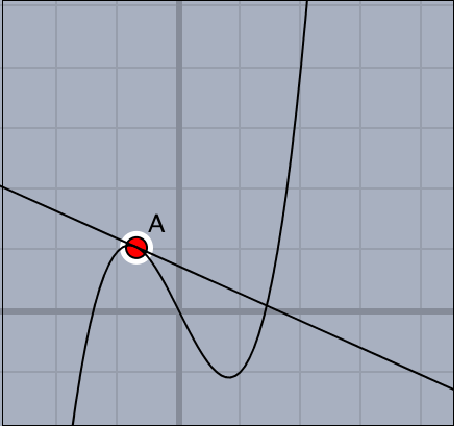
\includegraphics[bb=0.00 0.00 218.01 204.51,width=40mm]{Fig/ptselected01.pdf} 
\hspace{10mm}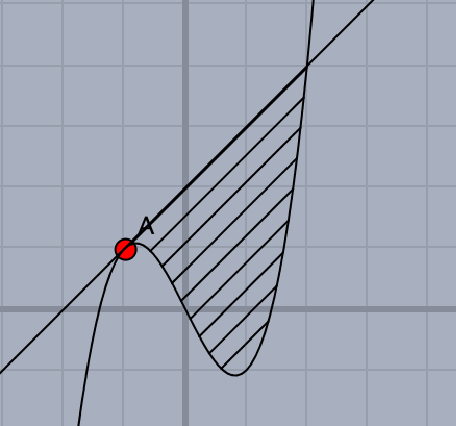
\includegraphics[bb=0.00 0.00 219.01 204.51,width=40mm]{Fig/ptselected02.pdf} 

\vspace{\baselineskip}
\hypertarget{slider}{}
\item[関数]  Slider(名称,位置1,位置2)
\item[機能]  スライダを作成する
\item[説明]  名称は "A-C-B" の形で,端点をA,B,スライダ点をCとしたスライダを作る。

端点A,Bの位置を,位置1,位置2で指定する。

スライダにより取得したい値は,点Cの座標(たとえば C.x)を利用する。

点A,B,Cはあらかじめ作図しておく必要はない。既にある場合はその点を使う。

\vspace{\baselineskip}
【例】2つのスライダを用意し,$y=a\sin(x-b)$ のa,b をインタラクティブに変化させる。
  
\verb|Slider("A-C-B",[-5,-2],[5,-2]);  | // \verb|C| is movable.\\
\verb|Slider("D-F-E",[-6,-2],[-6,2]);  | // \verb|F| is movable.\\
\verb|Plotdata("1",Assign("y=a*sin(x-b)",["a",F.y,"b",C.x]),"x"); |

\vspace{\baselineskip}
\hspace{15mm}
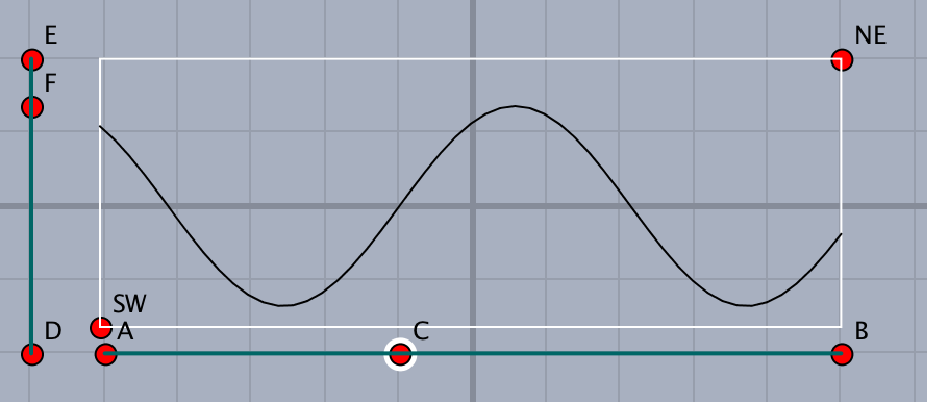
\includegraphics[bb=0.00 0.00 445.02 193.01,height=40mm]{Fig/slider.pdf} 

\begin{flushright}  \hyperlink{functionlist}{$\Rightarrow$関数一覧}\end{flushright}

\vspace{\baselineskip}
\hypertarget{sprintf}{}
\item[関数]  Sprintf(実数,長さ)
\item[機能]  小数点以下の長さを固定した文字列に変換
\item[説明]  実数を,小数点n位までの数とした文字列に変換する

\vspace{\baselineskip}
【例】円周率

 Sprintf(pi,2) は 3.14 を返す

 Sprintf(pi,7) は 3.1415927 を返す
    
注)pi は Cindyscriptの予約変数で,円周率を表す。\vspace{\baselineskip}

\vspace{\baselineskip}
\hypertarget{textformat}{}
\item[関数]  Textformat(数,桁数)
\item[機能]  小数点以下の桁数を指定して数を文字列化する。
\item[説明]  第1引数は数のリストでもよい。数のリストの場合は,戻り値は,対応する数値を指定係数にした後,リストを文字列化する。Cindyscriptの組み込み関数にも,format()という同様の関数があるが,format() は文字列のリストを返す。

\vspace{\baselineskip}
【例】円周率を小数点以下5位までで文字列化する。

\hspace{10mm} \verb|Textformat(pi,5);|
\hspace{10mm} \verb|format(pi,5);|
    
戻り値は,いずれも \verb|"3.14159"|

\vspace{\baselineskip}
【例】第1引数がリストのときの,format() との戻り値の違い。

\hspace{10mm} \verb|  dt=[1/6,0.5];|\\
\hspace{10mm} \verb|  Textformat(dt,4); | // 戻り値は "[ 0.1667 , 0.5 ]" \\
\hspace{10mm} \verb|  format(dt,4);     | // 戻り値は [ "0.1667" , "0.5" ] \\

\vspace{\baselineskip}
\hypertarget{texcom}{}
\item[関数]  Texcom(\TeX コード)
\item[機能]  \TeX のコードを書き出す
\item[説明]  任意の\TeX のコードを書き出す

\vspace{\baselineskip}
\hypertarget{windispg}{}
\item[関数]  Windispg()  または  Windisp(データのリスト)
\item[機能]  定義されているプロットデータをCinderella画面に黒線で描く
\item[説明]  Windispg()は,スクリプトの最後に置くことで,出力される部分だけが黒で描かれるので,出力図を確認することができる。ただし,Letter()関数で表示した点の名称などがCinderellaで作図したラベルと重なって表示されて見にくくなることもある。この関数を実行しなくても出力には影響しない。

Windisp(データのリスト)は,Rから \ketcindy 用に出力されたファイルを ReadOutData()関数で読み込んだときに,必要なプロットデータ列だけを表示するのに用いる。
  
ReadOutData("filename.txt") でデータを読み込むと,そのデータに含まれるプロットデータ列が,コンソールに

\hspace{10mm}Outdata of filename.txt : [Gfn,Gdfn,Gh] 

のように表示される。

このうち,GfnとGhだけを表示するのであれば

\hspace{10mm}\verb|Windispg([Gfn,Gh]);|

とする。引数なしで
 
\hspace{10mm}\verb|Windispg();|

とすればすべてのプロットデータ列が表示される。

なお,いずれの場合も,作図したプロットデータも同時に表示される。

作図した図を全てではなく選択して表示する場合は,それらのプロットデータ名をリストにして引数とする。

たとえば,sg1, gr1, crABが定義されているとき,

\hspace{10mm}\verb|Windispg(["sg1","gr1"]);|
        
とすれば,sg1,gr1のみが表示される。

%\begin{flushright}  \hyperlink{functionlist}{$\Rightarrow$関数一覧}\end{flushright}

\vspace{\baselineskip}
\hypertarget{viewtex}{}
\item[関数]  Viewtex()
\item[機能]  \TeX のソースファイルを書き出す。引数なし。
\item[説明]  グローバル変数Fheadで定義したファイル名に "main" を付加した\TeX のソースファイルとバッチファイル(Macの場合はシェルファイル)を作成する。
 
\vspace{\baselineskip}
\hypertarget{workprocess}{}
\item[関数]  Workprocess()
\item[機能]  作図の経過を取得する
\item[説明]  作図ツールを用いた作図の経過を取得する。

\verb|println(Workproccess());|
  
  とすると,コンソールに作図手順が表示される。

\vspace{\baselineskip}
\hypertarget{op}{}
\item[関数]  Op(n,list or str)
\item[機能]  リストまたは文字列から要素を抜き出す
\item[説明]  第2引数のリストまたは文字列のn番目の要素(文字)を返す。

Cindyscriptの アンダーバーの演算子 (list\_n , str\_n) と同様。

\vspace{\baselineskip}
\hypertarget{strsplit}{}
\item[関数]  Strsplit(文字列 , 文字)
\item[機能]  文字列を分解する。
\item[説明]  第1引数の文字列を第2引数の文字の位置で分解したリストを返す。

\vspace{\baselineskip}
【例】文字aで区切って分解する。

\verb|  str="abcadeaf";| \\
\verb|  strL=Strsplit(str,"a"); |  //  [” ”,”bc”,”de”,”f”] を返す。

同様の関数に,Cindyscriptの tokenize(文字列,文字列)がある。tokenize() の第2引数は文字列や,文字のリストでもよい。

\begin{flushright}  \hyperlink{functionlist}{$\Rightarrow$関数一覧}\end{flushright}


\end{description}
\newpage

%第11節 他の数式処理ソフトとの連携  =============================
\section{他の数式処理ソフトなどとの連携}
\subsection{Rとの連携}

Rは主に統計解析のためのソフトウェアで,  binorm(二項分布),pois(ポアソン),unif(一様分布),chisq(カイ2乗),f(F分布),t(t分布)など,多くの確率分布をサポートしている。

  \ketcindy では,kc.bat/shによってコマンドをRに渡し,結果をテキストファイルで受け取る。このとき,Rとのやりとりで,次のようなファイルが作業ディレクトリに作成される。
  
拡張子 r :r用のファイル

拡張子 dat,拡張子 txt:データファイル

このデータのやり取りに関する次のオプションがある。

  オプションなしまたは,”” のとき
  
    i) データファイルがなければ,新しく作る
    
    ii) データファイルが既にあればそれを読み込む
    
  "m"  のとき,強制的にデータファイルを作り直す。
  
  "r" のとき,すでにあるデータファイルを読み込む。
  
\vspace{\baselineskip}

\begin{description}

\hypertarget{boxplot}{}
\item[関数]  Boxplot(名前,データ,垂直位置,箱の高さ,option)
\item[機能]  箱ひげ図を描く
\item[説明]  データは,リストで渡す場合とファイル名を渡してファイルから読み込む場合がある。データファイルは csv 形式とする。

\vspace{\baselineskip}
【例】乱数で作成した5未満の実数のデータを箱ひげ図にする。

\begin{verbatim}
    dt1=apply(1..100,5*random());
    Boxplot("1",dt1,1,1/2);
\end{verbatim}
\vspace{\baselineskip}
\hspace{20mm} %%% /Users/Hannya/Desktop/fig/boxplot01.tex 
%%% Generator=hachtest.cdy 
{\unitlength=10mm%
\begin{picture}%
(5.91,2.32)(-0.38,-0.27)%
\special{pn 8}%
%
{%
\color[rgb]{0,0,0}%
\special{pa    21  -295}\special{pa    21  -492}%
\special{fp}%
}%
{%
\color[rgb]{0,0,0}%
\special{pa   338  -197}\special{pa   338  -591}\special{pa  1436  -591}\special{pa  1436  -197}%
\special{pa   338  -197}%
\special{fp}%
}%
{%
\color[rgb]{0,0,0}%
\special{pa  1962  -295}\special{pa  1962  -492}%
\special{fp}%
}%
{%
\color[rgb]{0,0,0}%
\special{pn 16}%
\special{pa   794  -197}\special{pa   794  -591}%
\special{fp}%
\special{pn 8}%
}%
{%
\color[rgb]{0,0,0}%
\special{pa 21 -394}\special{pa 56 -394}\special{fp}\special{pa 92 -394}\special{pa 127 -394}\special{fp}%
\special{pa 162 -394}\special{pa 197 -394}\special{fp}\special{pa 233 -394}\special{pa 268 -394}\special{fp}%
\special{pa 303 -394}\special{pa 338 -394}\special{fp}%
%
}%
{%
\color[rgb]{0,0,0}%
\special{pa 1436 -394}\special{pa 1471 -394}\special{fp}\special{pa 1506 -394}\special{pa 1541 -394}\special{fp}%
\special{pa 1576 -394}\special{pa 1611 -394}\special{fp}\special{pa 1646 -394}\special{pa 1681 -394}\special{fp}%
\special{pa 1717 -394}\special{pa 1752 -394}\special{fp}\special{pa 1787 -394}\special{pa 1822 -394}\special{fp}%
\special{pa 1857 -394}\special{pa 1892 -394}\special{fp}\special{pa 1927 -394}\special{pa 1962 -394}\special{fp}%
%
%
}%
\special{pa  -150    -0}\special{pa  2177    -0}%
\special{fp}%
\special{pa     0   106}\special{pa     0  -807}%
\special{fp}%
\settowidth{\Width}{$x$}\setlength{\Width}{0\Width}%
\settoheight{\Height}{$x$}\settodepth{\Depth}{$x$}\setlength{\Height}{-0.5\Height}\setlength{\Depth}{0.5\Depth}\addtolength{\Height}{\Depth}%
\put(5.5800000,0.0000000){\hspace*{\Width}\raisebox{\Height}{$x$}}%
%
\settowidth{\Width}{$y$}\setlength{\Width}{-0.5\Width}%
\settoheight{\Height}{$y$}\settodepth{\Depth}{$y$}\setlength{\Height}{\Depth}%
\put(0.0000000,2.1000000){\hspace*{\Width}\raisebox{\Height}{$y$}}%
%
\settowidth{\Width}{O}\setlength{\Width}{-1\Width}%
\settoheight{\Height}{O}\settodepth{\Depth}{O}\setlength{\Height}{-\Height}%
\put(-0.0500000,-0.0500000){\hspace*{\Width}\raisebox{\Height}{O}}%
%
\end{picture}}%

\vspace{\baselineskip}
【例】外部ファイルとして用意したデータを読み込んで箱ひげ図にする。
\begin{verbatim}
    Boxplot("2","datafile.csv",3,1/2);
\end{verbatim}

\vspace{\baselineskip}
複数列から成るcsvファイルを読み込むには,Readcsvを使う。csvファイルは,作業フォルダ( 初期設定は fig )に入れておく。戻り値は読み込んだファイル。
  
データの値を画面に入るように調節するには,dt1/20 のようにしてリサイズする。
 
また,Framedata(),Rulerscale() を併用することで目盛を入れることができる。Framedata() のために,表示領域の対角点A,BをCinderellaの作図ツールで作図しておく。

\begin{verbatim}
    data=Readcsv("datafile.csv");
    dt1=apply(data,#_1);
    dt2=apply(data,#_2);
    Boxplot("1",dt1/20,1,1/2);
    Boxplot("2",dt2/20,3,1/2);
    Framedata("1",[A,B],["corner"]);
    Rulerscale(A,["r",0,6,1],["f",1,"\mbox{dt1}",3,"\mbox{dt2}"]);
\end{verbatim}
%\vspace{\baselineskip}
 \begin{center} %%% t4boxplot2.tex 2016-4-23 9:27
%%% t4boxplot2.sce 2016-4-23 9:27
{\unitlength=1cm%
\begin{picture}%
(   8.00000,   6.00000)(  -1.00000,  -1.00000)%
\special{pn 8}%
%
\special{pa 394 -295}\special{pa 394 -492}%
\special{fp}%
\special{pa 1181 -197}\special{pa 1181 -591}\special{pa 1713 -591}\special{pa 1713 -197}%
\special{pa 1181 -197}%
\special{fp}%
\special{pa 1949 -295}\special{pa 1949 -492}%
\special{fp}%
\special{pn 16}%
\special{pa 1378 -197}\special{pa 1378 -591}%
\special{fp}%
\special{pn 8}%
\special{pa 394 -394}\special{pa 431 -394}\special{fp}\special{pa 469 -394}\special{pa 506 -394}\special{fp}%
\special{pa 544 -394}\special{pa 581 -394}\special{fp}\special{pa 619 -394}\special{pa 656 -394}\special{fp}%
\special{pa 694 -394}\special{pa 731 -394}\special{fp}\special{pa 769 -394}\special{pa 806 -394}\special{fp}%
\special{pa 844 -394}\special{pa 881 -394}\special{fp}\special{pa 919 -394}\special{pa 956 -394}\special{fp}%
\special{pa 994 -394}\special{pa 1031 -394}\special{fp}\special{pa 1069 -394}\special{pa 1106 -394}\special{fp}%
\special{pa 1144 -394}\special{pa 1181 -394}\special{fp}%
%
\special{pa 1713 -394}\special{pa 1746 -394}\special{fp}\special{pa 1780 -394}\special{pa 1814 -394}\special{fp}%
\special{pa 1848 -394}\special{pa 1881 -394}\special{fp}\special{pa 1915 -394}\special{pa 1949 -394}\special{fp}%
%
%
\special{pa 787 -1083}\special{pa 787 -1280}%
\special{fp}%
\special{pa 1299 -984}\special{pa 1299 -1378}\special{pa 1673 -1378}\special{pa 1673 -984}%
\special{pa 1299 -984}%
\special{fp}%
\special{pa 1969 -1083}\special{pa 1969 -1280}%
\special{fp}%
\special{pn 16}%
\special{pa 1378 -984}\special{pa 1378 -1378}%
\special{fp}%
\special{pn 8}%
\special{pa 787 -1181}\special{pa 827 -1181}\special{fp}\special{pa 866 -1181}\special{pa 906 -1181}\special{fp}%
\special{pa 945 -1181}\special{pa 984 -1181}\special{fp}\special{pa 1024 -1181}\special{pa 1063 -1181}\special{fp}%
\special{pa 1102 -1181}\special{pa 1142 -1181}\special{fp}\special{pa 1181 -1181}\special{pa 1220 -1181}\special{fp}%
\special{pa 1260 -1181}\special{pa 1299 -1181}\special{fp}%
%
\special{pa 1673 -1181}\special{pa 1706 -1181}\special{fp}\special{pa 1739 -1181}\special{pa 1772 -1181}\special{fp}%
\special{pa 1804 -1181}\special{pa 1837 -1181}\special{fp}\special{pa 1870 -1181}\special{pa 1903 -1181}\special{fp}%
\special{pa 1936 -1181}\special{pa 1969 -1181}\special{fp}%
%
\special{pa 0 0}\special{pa 2386 0}\special{pa 2386 -1709}\special{pa 0 -1709}\special{pa 0 0}%
\special{fp}%
\settowidth{\Width}{$0$}\setlength{\Width}{-0.5\Width}%
\settoheight{\Height}{$0$}\settodepth{\Depth}{$0$}\setlength{\Height}{-\Height}%
\put(0.0000,-0.1500){\hspace*{\Width}\raisebox{\Height}{$0$}}%
%
%
\special{pa 0 0}\special{pa 0 39}%
\special{fp}%
\settowidth{\Width}{$1$}\setlength{\Width}{-0.5\Width}%
\settoheight{\Height}{$1$}\settodepth{\Depth}{$1$}\setlength{\Height}{-\Height}%
\put(1.0000,-0.1500){\hspace*{\Width}\raisebox{\Height}{$1$}}%
%
%
\special{pa 394 0}\special{pa 394 39}%
\special{fp}%
\settowidth{\Width}{$2$}\setlength{\Width}{-0.5\Width}%
\settoheight{\Height}{$2$}\settodepth{\Depth}{$2$}\setlength{\Height}{-\Height}%
\put(2.0000,-0.1500){\hspace*{\Width}\raisebox{\Height}{$2$}}%
%
%
\special{pa 787 0}\special{pa 787 39}%
\special{fp}%
\settowidth{\Width}{$3$}\setlength{\Width}{-0.5\Width}%
\settoheight{\Height}{$3$}\settodepth{\Depth}{$3$}\setlength{\Height}{-\Height}%
\put(3.0000,-0.1500){\hspace*{\Width}\raisebox{\Height}{$3$}}%
%
%
\special{pa 1181 0}\special{pa 1181 39}%
\special{fp}%
\settowidth{\Width}{$4$}\setlength{\Width}{-0.5\Width}%
\settoheight{\Height}{$4$}\settodepth{\Depth}{$4$}\setlength{\Height}{-\Height}%
\put(4.0000,-0.1500){\hspace*{\Width}\raisebox{\Height}{$4$}}%
%
%
\special{pa 1575 0}\special{pa 1575 39}%
\special{fp}%
\settowidth{\Width}{$5$}\setlength{\Width}{-0.5\Width}%
\settoheight{\Height}{$5$}\settodepth{\Depth}{$5$}\setlength{\Height}{-\Height}%
\put(5.0000,-0.1500){\hspace*{\Width}\raisebox{\Height}{$5$}}%
%
%
\special{pa 1969 0}\special{pa 1969 39}%
\special{fp}%
\settowidth{\Width}{$6$}\setlength{\Width}{-0.5\Width}%
\settoheight{\Height}{$6$}\settodepth{\Depth}{$6$}\setlength{\Height}{-\Height}%
\put(6.0000,-0.1500){\hspace*{\Width}\raisebox{\Height}{$6$}}%
%
%
\special{pa 2362 0}\special{pa 2362 39}%
\special{fp}%
\settowidth{\Width}{$\mbox{dt1}$}\setlength{\Width}{-1\Width}%
\settoheight{\Height}{$\mbox{dt1}$}\settodepth{\Depth}{$\mbox{dt1}$}\setlength{\Height}{-0.5\Height}\setlength{\Depth}{0.5\Depth}\addtolength{\Height}{\Depth}%
\put(-0.1500,1.0000){\hspace*{\Width}\raisebox{\Height}{$\mbox{dt1}$}}%
%
%
\special{pa 0 -394}\special{pa -39 -394}%
\special{fp}%
\settowidth{\Width}{$\mbox{dt2}$}\setlength{\Width}{-1\Width}%
\settoheight{\Height}{$\mbox{dt2}$}\settodepth{\Depth}{$\mbox{dt2}$}\setlength{\Height}{-0.5\Height}\setlength{\Depth}{0.5\Depth}\addtolength{\Height}{\Depth}%
\put(-0.1500,3.0000){\hspace*{\Width}\raisebox{\Height}{$\mbox{dt2}$}}%
%
%
\special{pa 0 -1181}\special{pa -39 -1181}%
\special{fp}%
\end{picture}}% \end{center}

注)一度実行した後,データを書き直すと,図が更新されないので,"m" オプションをつけて
    Boxplot("1",dt1/20,1,1/2,["m"]); とすると,図が更新される。データを書き出すときは,もう一度 "m" オプションをはずして実行してから Figure ボタンを押す。これは,データの作成タイミングの関係。

\begin{flushright}  \hyperlink{functionlist}{$\Rightarrow$関数一覧}\end{flushright}

\hypertarget{rfun}{}
\item[関数]  Rfun(name,コマンド, 引数, option)
\item[機能]  Rの1つのコマンドを実行して結果を返す
\item[説明]  バッチファイル kc.bat / シェルファイル kc.sh を利用してRとデータをやり取りし,計算結果を取得する。結果は,変数 R+name に入り,コンソールにも表示される。

\vspace{\baselineskip}
【例】Rを用いて標準正規分布から10個の乱数を発生し,戻り値から平均値と標準偏差を求めてコンソールに表示する。
\begin{verbatim}
    Rfun("1","rnorm",[10]);
    nx=length(R1);
    mx=sum(R1)/nx;
    sx=sqrt(R1*R1/nx-mx^2);
    println("平均:"+format(mx,4)+"    標準偏差:"+format(sx,4));
\end{verbatim}

\hypertarget{calcbyr}{}
\item[関数]  CalcbyR(変数名,コマンド列,option)
\item[機能]  Rのコマンドを実行して結果を返す
\item[説明]  バッチファイル kc.bat / シェルファイル kc.sh を利用してRとデータをやり取りし,計算結果を取得する。

    コマンド列は,"戻り値=コマンド",[引数] の2つをセットとして並べる。
    
    最後の行の結果が戻り値として第1引数の変数名に代入される。"戻り値1::戻り値2・・",[]  の形(戻り値1,戻り値2・・は各コマンドの戻り値)でコマンドを書くと,戻り値1,・・のリストとなる。戻り値が一つの場合は実数。"=値",[] の形の場合,「値」がそのまま戻り値となる。

\vspace{\baselineskip}
【例】Rを用いてN(50,$5^2$)から10個の乱数を発生し,平均と不偏分散もRで計算してその結果をコンソールに表示する。
\begin{verbatim}
    cmdL=[
        "tmp1=rnorm",[10,50,5],
        "tmp2=mean",["tmp1"],
        "tmp3=var",["tmp1"],
        "tmp1::tmp2::tmp3",[]
    ];
    CalcbyR("rd",cmdL);
    dt=rd_1;
    mx=rd_2;
    vx=rd_3;
    println("データ:"+dt);
    println("平均:"+format(mx,4)+"    不偏分散:"+format(vx,4));
\end{verbatim}
  CalcbyR()によって,データと平均,不偏分散からなるリストが作成されるので,mxに平均,vxに不偏分散を代入している。\verb|rd_(-1)| は,リスト rd の末尾の要素。
  
\vspace{\baselineskip}
【例】Rでポアソン分布から200個の乱数をとり,標本平均の分布の様子=分散が小さくなって,正規分布に近づいている様子=をヒストグラムで見る。分散はRで求めた不偏分散に (n-1)/n をかけて再計算してコンソールに表示する。
\begin{verbatim}
    cmdL=[
      "tmp1=rpois",[200,5],
      "tmp2=mean",["tmp1"],
      "tmp3=var",["tmp1"],
      "=c(tmp2,tmp3,tmp1)",[]
    ];
    CalcbyR("rd",cmdL);
    dt=rd_(3..length(rd));
    n=length(dt);
    mx=rd_1;
    vx=rd_2*(n-1)/n;
    sx=sqrt(vx);
    println(dt);
    println(["m="+format(mx,4),"v="+format(vx,4)]);
    Setscaling(1/5);
    Histplot("1",dt,["Breaks=seq(0,14,1)","dr,0.5"]);
\end{verbatim}
\vspace{\baselineskip}
          \begin{center} %%% fig.tex 2016-4-23 10:42
%%% fig.sce 2016-4-23 10:41
{\unitlength=5mm%
\begin{picture}%
(  14.89000,   9.57800)(  -0.82000,  -0.77000)%
\special{pn 8}%
%
\special{pn 4}%
\special{pa 0 0}\special{pa 0 -236}\special{pa 197 -236}\special{pa 197 0}\special{pa 0 0}%
\special{fp}%
\special{pn 8}%
\special{pn 4}%
\special{pa 197 0}\special{pa 197 -748}\special{pa 394 -748}\special{pa 394 0}\special{pa 197 0}%
\special{fp}%
\special{pn 8}%
\special{pn 4}%
\special{pa 394 0}\special{pa 394 -1181}\special{pa 591 -1181}\special{pa 591 0}\special{pa 394 0}%
\special{fp}%
\special{pn 8}%
\special{pn 4}%
\special{pa 591 0}\special{pa 591 -1457}\special{pa 787 -1457}\special{pa 787 0}\special{pa 591 0}%
\special{fp}%
\special{pn 8}%
\special{pn 4}%
\special{pa 787 0}\special{pa 787 -1339}\special{pa 984 -1339}\special{pa 984 0}\special{pa 787 0}%
\special{fp}%
\special{pn 8}%
\special{pn 4}%
\special{pa 984 0}\special{pa 984 -1063}\special{pa 1181 -1063}\special{pa 1181 0}%
\special{pa 984 0}%
\special{fp}%
\special{pn 8}%
\special{pn 4}%
\special{pa 1181 0}\special{pa 1181 -827}\special{pa 1378 -827}\special{pa 1378 0}%
\special{pa 1181 0}%
\special{fp}%
\special{pn 8}%
\special{pn 4}%
\special{pa 1378 0}\special{pa 1378 -512}\special{pa 1575 -512}\special{pa 1575 0}%
\special{pa 1378 0}%
\special{fp}%
\special{pn 8}%
\special{pn 4}%
\special{pa 1575 0}\special{pa 1575 -394}\special{pa 1772 -394}\special{pa 1772 0}%
\special{pa 1575 0}%
\special{fp}%
\special{pn 8}%
\special{pn 4}%
\special{pa 1772 0}\special{pa 1969 0}\special{pa 1772 0}%
\special{fp}%
\special{pn 8}%
\special{pn 4}%
\special{pa 1969 0}\special{pa 1969 -79}\special{pa 2165 -79}\special{pa 2165 0}\special{pa 1969 0}%
\special{fp}%
\special{pn 8}%
\special{pn 4}%
\special{pa 2165 0}\special{pa 2165 -39}\special{pa 2362 -39}\special{pa 2362 0}\special{pa 2165 0}%
\special{fp}%
\special{pn 8}%
\special{pn 4}%
\special{pa 2362 0}\special{pa 2559 0}\special{pa 2362 0}%
\special{fp}%
\special{pn 8}%
\special{pn 4}%
\special{pa 2559 0}\special{pa 2756 0}\special{pa 2559 0}%
\special{fp}%
\special{pn 8}%
\special{pa -161 0}\special{pa 2770 0}%
\special{fp}%
\special{pa 0 152}\special{pa 0 -1734}%
\special{fp}%
\settowidth{\Width}{$x$}\setlength{\Width}{0\Width}%
\settoheight{\Height}{$x$}\settodepth{\Depth}{$x$}\setlength{\Height}{-0.5\Height}\setlength{\Depth}{0.5\Depth}\addtolength{\Height}{\Depth}%
\put(14.1200,0.0000){\hspace*{\Width}\raisebox{\Height}{$x$}}%
%
%
\settowidth{\Width}{$y$}\setlength{\Width}{-0.5\Width}%
\settoheight{\Height}{$y$}\settodepth{\Depth}{$y$}\setlength{\Height}{\Depth}%
\put(0.0000,8.8580){\hspace*{\Width}\raisebox{\Height}{$y$}}%
%
%
\settowidth{\Width}{O}\setlength{\Width}{-1\Width}%
\settoheight{\Height}{O}\settodepth{\Depth}{O}\setlength{\Height}{-\Height}%
\put(-0.0500,-0.0500){\hspace*{\Width}\raisebox{\Height}{O}}%
%
%
\end{picture}}% \end{center}
\vspace{\baselineskip}
【例】ポアソン分布で乱数を2000個発生させ,10個ずつの平均をRで計算し,ヒストグラムを作る。
\begin{verbatim}
    cmdL=[
      "tmp1=rpois",[2000,5],
      "tmp2=c()",[],
      "for(k in 1:200){",[],
      "  tmp=tmp1[(10*(k-1)+1):(10*k)]",[],
      "  tmp2=c(tmp2,mean(tmp))",[],
      "}",[],
      "=tmp2",[]
    ];
    CalcbyR("rd2",cmdL);
    Setscaling(1/10);
    Histplot("2",rd2);
\end{verbatim}

\begin{flushright}  \hyperlink{functionlist}{$\Rightarrow$関数一覧}\end{flushright}
\hypertarget{histplot}{}
\item[関数]  Histplot(name,data,option)
\item[機能]  Rを利用してヒストグラムを描く
\item[説明]  dataはリストにして作成するか,外部ファイルからReadcsv()で読み込む。

階級境界値(ブレークポイント)は,自動的に設定される(スタージェスの公式による)が,オプションで,

\verb|"breaks=[0,10,20,30,40,50,60,70,80,90,100]"|
      
などと指定することもできる。

  この他のオプションは
  
    "Den=yes/no":密度の指定(初期値は no)
    
    "Rel=yes/no":相対度数にする/しない(初期値は no)
    
\vspace{\baselineskip}
【例】csvファイル(datafile.csv)を読み込み,ヒストグラムを作る。Framedata() と Rulerscale()を併用して,目盛付きの枠の中に表示する。表示枠の対角点A,BはCinderellaの作図ツールで作図しておく。
\begin{verbatim}
    Addax(0);
    Setscaling(5);
    Setunitlen("0.6mm");
    data=Readcsv("datafile.csv");
    Histplot("1",data,[""]);
    Framedata("1",[A,B],["corner"]);
    Rulerscale(A,["r",0,100,10],["r",0,15,5]);
\end{verbatim}
    \begin{center} %%% t5histplot.tex 2016-4-23 11:21
%%% t5histplot.sce 2016-4-23 11:21
{\unitlength=0.6mm%
\begin{picture}%
( 132.11000,  89.65000)( -18.31000,  -8.10000)%
\special{pn 8}%
%
\special{pa 472 0}\special{pa 472 -709}\special{pa 709 -709}\special{pa 709 0}\special{pa 472 0}%
\special{fp}%
\special{pa 709 0}\special{pa 709 -236}\special{pa 945 -236}\special{pa 945 0}\special{pa 709 0}%
\special{fp}%
\special{pa 945 0}\special{pa 1181 0}\special{pa 945 0}%
\special{fp}%
\special{pa 1181 0}\special{pa 1181 -1654}\special{pa 1417 -1654}\special{pa 1417 0}%
\special{pa 1181 0}%
\special{fp}%
\special{pa 1417 0}\special{pa 1417 -945}\special{pa 1654 -945}\special{pa 1654 0}%
\special{pa 1417 0}%
\special{fp}%
\special{pa 1654 0}\special{pa 1654 -827}\special{pa 1890 -827}\special{pa 1890 0}%
\special{pa 1654 0}%
\special{fp}%
\special{pa 1890 0}\special{pa 1890 -1654}\special{pa 2126 -1654}\special{pa 2126 0}%
\special{pa 1890 0}%
\special{fp}%
\special{pa 2126 0}\special{pa 2126 -827}\special{pa 2362 -827}\special{pa 2362 0}%
\special{pa 2126 0}%
\special{fp}%
\special{pa -118 0}\special{pa 2480 0}\special{pa 2480 -1772}\special{pa -118 -1772}%
\special{pa -118 0}%
\special{fp}%
\settowidth{\Width}{$0$}\setlength{\Width}{-0.5\Width}%
\settoheight{\Height}{$0$}\settodepth{\Depth}{$0$}\setlength{\Height}{-\Height}%
\put(0.0000,-0.1500){\hspace*{\Width}\raisebox{\Height}{$0$}}%
%
%
\special{pa 0 0}\special{pa 0 2}%
\special{fp}%
\settowidth{\Width}{$10$}\setlength{\Width}{-0.5\Width}%
\settoheight{\Height}{$10$}\settodepth{\Depth}{$10$}\setlength{\Height}{-\Height}%
\put(10.0000,-0.1500){\hspace*{\Width}\raisebox{\Height}{$10$}}%
%
%
\special{pa 236 0}\special{pa 236 2}%
\special{fp}%
\settowidth{\Width}{$20$}\setlength{\Width}{-0.5\Width}%
\settoheight{\Height}{$20$}\settodepth{\Depth}{$20$}\setlength{\Height}{-\Height}%
\put(20.0000,-0.1500){\hspace*{\Width}\raisebox{\Height}{$20$}}%
%
%
\special{pa 472 0}\special{pa 472 2}%
\special{fp}%
\settowidth{\Width}{$30$}\setlength{\Width}{-0.5\Width}%
\settoheight{\Height}{$30$}\settodepth{\Depth}{$30$}\setlength{\Height}{-\Height}%
\put(30.0000,-0.1500){\hspace*{\Width}\raisebox{\Height}{$30$}}%
%
%
\special{pa 709 0}\special{pa 709 2}%
\special{fp}%
\settowidth{\Width}{$40$}\setlength{\Width}{-0.5\Width}%
\settoheight{\Height}{$40$}\settodepth{\Depth}{$40$}\setlength{\Height}{-\Height}%
\put(40.0000,-0.1500){\hspace*{\Width}\raisebox{\Height}{$40$}}%
%
%
\special{pa 945 0}\special{pa 945 2}%
\special{fp}%
\settowidth{\Width}{$50$}\setlength{\Width}{-0.5\Width}%
\settoheight{\Height}{$50$}\settodepth{\Depth}{$50$}\setlength{\Height}{-\Height}%
\put(50.0000,-0.1500){\hspace*{\Width}\raisebox{\Height}{$50$}}%
%
%
\special{pa 1181 0}\special{pa 1181 2}%
\special{fp}%
\settowidth{\Width}{$60$}\setlength{\Width}{-0.5\Width}%
\settoheight{\Height}{$60$}\settodepth{\Depth}{$60$}\setlength{\Height}{-\Height}%
\put(60.0000,-0.1500){\hspace*{\Width}\raisebox{\Height}{$60$}}%
%
%
\special{pa 1417 0}\special{pa 1417 2}%
\special{fp}%
\settowidth{\Width}{$70$}\setlength{\Width}{-0.5\Width}%
\settoheight{\Height}{$70$}\settodepth{\Depth}{$70$}\setlength{\Height}{-\Height}%
\put(70.0000,-0.1500){\hspace*{\Width}\raisebox{\Height}{$70$}}%
%
%
\special{pa 1654 0}\special{pa 1654 2}%
\special{fp}%
\settowidth{\Width}{$80$}\setlength{\Width}{-0.5\Width}%
\settoheight{\Height}{$80$}\settodepth{\Depth}{$80$}\setlength{\Height}{-\Height}%
\put(80.0000,-0.1500){\hspace*{\Width}\raisebox{\Height}{$80$}}%
%
%
\special{pa 1890 0}\special{pa 1890 2}%
\special{fp}%
\settowidth{\Width}{$90$}\setlength{\Width}{-0.5\Width}%
\settoheight{\Height}{$90$}\settodepth{\Depth}{$90$}\setlength{\Height}{-\Height}%
\put(90.0000,-0.1500){\hspace*{\Width}\raisebox{\Height}{$90$}}%
%
%
\special{pa 2126 0}\special{pa 2126 2}%
\special{fp}%
\settowidth{\Width}{$100$}\setlength{\Width}{-0.5\Width}%
\settoheight{\Height}{$100$}\settodepth{\Depth}{$100$}\setlength{\Height}{-\Height}%
\put(100.0000,-0.1500){\hspace*{\Width}\raisebox{\Height}{$100$}}%
%
%
\special{pa 2362 0}\special{pa 2362 2}%
\special{fp}%
\settowidth{\Width}{$0$}\setlength{\Width}{-1\Width}%
\settoheight{\Height}{$0$}\settodepth{\Depth}{$0$}\setlength{\Height}{-0.5\Height}\setlength{\Depth}{0.5\Depth}\addtolength{\Height}{\Depth}%
\put(-5.1500,0.0000){\hspace*{\Width}\raisebox{\Height}{$0$}}%
%
%
\special{pa -118 0}\special{pa -120 0}%
\special{fp}%
\settowidth{\Width}{$5$}\setlength{\Width}{-1\Width}%
\settoheight{\Height}{$5$}\settodepth{\Depth}{$5$}\setlength{\Height}{-0.5\Height}\setlength{\Depth}{0.5\Depth}\addtolength{\Height}{\Depth}%
\put(-5.1500,25.0000){\hspace*{\Width}\raisebox{\Height}{$5$}}%
%
%
\special{pa -118 -591}\special{pa -120 -591}%
\special{fp}%
\settowidth{\Width}{$10$}\setlength{\Width}{-1\Width}%
\settoheight{\Height}{$10$}\settodepth{\Depth}{$10$}\setlength{\Height}{-0.5\Height}\setlength{\Depth}{0.5\Depth}\addtolength{\Height}{\Depth}%
\put(-5.1500,50.0000){\hspace*{\Width}\raisebox{\Height}{$10$}}%
%
%
\special{pa -118 -1181}\special{pa -120 -1181}%
\special{fp}%
\settowidth{\Width}{$15$}\setlength{\Width}{-1\Width}%
\settoheight{\Height}{$15$}\settodepth{\Depth}{$15$}\setlength{\Height}{-0.5\Height}\setlength{\Depth}{0.5\Depth}\addtolength{\Height}{\Depth}%
\put(-5.1500,75.0000){\hspace*{\Width}\raisebox{\Height}{$15$}}%
%
%
\special{pa -118 -1772}\special{pa -120 -1772}%
\special{fp}%
\end{picture}}% \end{center}

2行目と3行目は,データに合わせて縦方向を5倍にし,TeXの単位長を0.6mmにしている。

Den,Rel オプションをyes にしたときは,Setscaling(100)くらいにするのがよい。

csvファイルが複数のデータからなる場合は,

    \verb|dt1=data_1;|
として,リストの第1要素を取得する。第2要素のヒストグラムであれば  \verb|data_2| とする。

\vspace{\baselineskip}
\begin{flushright}  \hyperlink{functionlist}{$\Rightarrow$関数一覧}\end{flushright}

\hypertarget{plotdatar}{}
\item[関数]  PlotdataR(name,式,変数)
\item[機能]  Rの関数のグラフを描く
\item[説明]  Cindyscriptの組み込み関数にはない関数のグラフをRを利用して描く。

\vspace{\baselineskip}
【例】平均5, 標準偏差2の正規分布の密度関数と分布関数のグラフを描く。
\begin{verbatim}
    PlotdataR(“1”, “dnorm(x,5,2)”, ”x=[0,10]”);
    PlotdataR(“2”, ”pnorm(x,5,2)”, ”x=[0,10]”);
\end{verbatim}

\hspace{20mm} %%% /Users/Hannya/Desktop/fig/plotdatar1.tex 
%%% Generator=hachtest.cdy 
{\unitlength=8mm%
\begin{picture}%
(11.77,3.16)(-1,-1)%
\special{pn 8}%
%
{%
\color[rgb]{0,0,0}%
\special{pa     0    -3}\special{pa    63    -4}\special{pa   126    -4}\special{pa   189    -6}%
\special{pa   252    -7}\special{pa   315    -9}\special{pa   378   -10}\special{pa   441   -12}%
\special{pa   504   -15}\special{pa   567   -17}\special{pa   630   -20}\special{pa   693   -24}%
\special{pa   756   -27}\special{pa   819   -31}\special{pa   882   -34}\special{pa   945   -38}%
\special{pa  1008   -42}\special{pa  1071   -46}\special{pa  1134   -49}\special{pa  1197   -52}%
\special{pa  1260   -55}\special{pa  1323   -58}\special{pa  1386   -60}\special{pa  1449   -62}%
\special{pa  1512   -63}\special{pa  1575   -63}\special{pa  1638   -63}\special{pa  1701   -62}%
\special{pa  1764   -60}\special{pa  1827   -58}\special{pa  1890   -55}\special{pa  1953   -52}%
\special{pa  2016   -49}\special{pa  2079   -46}\special{pa  2142   -42}\special{pa  2205   -38}%
\special{pa  2268   -34}\special{pa  2331   -31}\special{pa  2394   -27}\special{pa  2457   -24}%
\special{pa  2520   -20}\special{pa  2583   -17}\special{pa  2646   -15}\special{pa  2709   -12}%
\special{pa  2772   -10}\special{pa  2835    -9}\special{pa  2898    -7}\special{pa  2961    -6}%
\special{pa  3024    -4}\special{pa  3087    -4}\special{pa  3150    -3}%
\special{fp}%
}%
{%
\color[rgb]{0,0,0}%
\special{pa     0    -2}\special{pa    63    -3}\special{pa   126    -3}\special{pa   189    -4}%
\special{pa   252    -6}\special{pa   315    -7}\special{pa   378    -9}\special{pa   441   -11}%
\special{pa   504   -14}\special{pa   567   -17}\special{pa   630   -21}\special{pa   693   -25}%
\special{pa   756   -30}\special{pa   819   -36}\special{pa   882   -43}\special{pa   945   -50}%
\special{pa  1008   -58}\special{pa  1071   -67}\special{pa  1134   -76}\special{pa  1197   -86}%
\special{pa  1260   -97}\special{pa  1323  -109}\special{pa  1386  -120}\special{pa  1449  -133}%
\special{pa  1512  -145}\special{pa  1575  -157}\special{pa  1638  -170}\special{pa  1701  -182}%
\special{pa  1764  -195}\special{pa  1827  -206}\special{pa  1890  -218}\special{pa  1953  -229}%
\special{pa  2016  -239}\special{pa  2079  -248}\special{pa  2142  -257}\special{pa  2205  -265}%
\special{pa  2268  -272}\special{pa  2331  -279}\special{pa  2394  -284}\special{pa  2457  -290}%
\special{pa  2520  -294}\special{pa  2583  -298}\special{pa  2646  -301}\special{pa  2709  -304}%
\special{pa  2772  -306}\special{pa  2835  -308}\special{pa  2898  -309}\special{pa  2961  -311}%
\special{pa  3024  -312}\special{pa  3087  -312}\special{pa  3150  -313}%
\special{fp}%
}%
\special{pa  -315    -0}\special{pa  3392    -0}%
\special{fp}%
\special{pa     0   315}\special{pa     0  -680}%
\special{fp}%
\settowidth{\Width}{$x$}\setlength{\Width}{0\Width}%
\settoheight{\Height}{$x$}\settodepth{\Depth}{$x$}\setlength{\Height}{-0.5\Height}\setlength{\Depth}{0.5\Depth}\addtolength{\Height}{\Depth}%
\put(10.8325000,0.0000000){\hspace*{\Width}\raisebox{\Height}{$x$}}%
%
\settowidth{\Width}{$y$}\setlength{\Width}{-0.5\Width}%
\settoheight{\Height}{$y$}\settodepth{\Depth}{$y$}\setlength{\Height}{\Depth}%
\put(0.0000000,2.2225000){\hspace*{\Width}\raisebox{\Height}{$y$}}%
%
\settowidth{\Width}{O}\setlength{\Width}{-1\Width}%
\settoheight{\Height}{O}\settodepth{\Depth}{O}\setlength{\Height}{-\Height}%
\put(-0.0625000,-0.0625000){\hspace*{\Width}\raisebox{\Height}{O}}%
%
\end{picture}}%

【例】標準正規分布のグラフ上の点とx軸を結んだ線分を描く。

点A,BはCinderellaの作図ツールで作図しておき,点Aをグラフ上のおよその位置に置いてから実行する。
\begin{verbatim}
    PlotdataR("1","dnorm(x)","x=[-5,5]");
    PutonCurve("A","grR1",[-3,3]);
    Putpoint("B",[A.x,0]);
    Listplot("1",[A,B]);
\end{verbatim}
2行目の最後の引数の[-3,3]は,その範囲を動かすことを意味する。

Aはグラフ上を動かすことができて,Bはそれに伴って動く。ただし,少し動かす度に バッチ/シェル ファイルを実行するので,煩雑な場合は,Plotdata() の行をコメント化してから点Aを動かしたあと再実行するとよい。

\vspace{\baselineskip}
【例】上と同様で,x軸上の点を自由点Aとし,曲線上にBを置く。
\begin{verbatim}
    PlotdataR("1","dnorm(x)","x=[-5,5]");
    PlotdataR("1","dnorm(x)","x=[-5,5]");
    A.xy=[A.x,0];
    Lineplot("1",[A,A+[0,1]],["nodisp"]);
    Putintersect("B","grR1","ln1");
    Listplot("1",[A,B]);
\end{verbatim}
\vspace{\baselineskip}
【例】前の例のグラフで,ABの左側にShadeをかけ,Shadeの部分の面積を求める。Pの値を表示する位置に,Cinderellaの作図ツールで点Cをとっておく。
\begin{verbatim}
    PlotdataR("1","dnorm(x)","x=[-5,5]",["Num=100"]);
    Putpoint("A",[0,0],[A.x,0]);
    Lineplot("1",[A,A+[0,1]],["nodisp"]);
    Putintersect("B","grR1","ln1");
    Listplot("1",[A,B]);
    Listplot("2",[[-5,0],[5,0]],"nodisp");
    Enclosing("1",["Invert(grR1)","sg2","sg1"],[B,"notex"]);
    Shade(["en1"],["Color=[0.2,0,0,0]"]);
    tmp=0.5+Integrate("grR1",[0,A.x]);
    Expr([A,"s",text(A.x),C,"e","P="+text(tmp)]);
\end{verbatim}

    \begin{center} %%% fig.tex 2016-4-23 15:15
%%% fig.sce 2016-4-23 15:15
{\unitlength=10mm%
\begin{picture}%
(   6.00000,   3.00000)(  -3.00000,  -1.00000)%
\special{pn 8}%
%
\color[cmyk]{0.2,0,0,0}%
\color[cmyk]{0.2,0,0,0}%
\special{pa 147 -293}\special{pa 139 -295}\special{pa 99 -304}\special{pa 60 -311}%
\special{pa 20 -314}\special{pa -20 -314}\special{pa -60 -311}\special{pa -99 -304}%
\special{pa -139 -295}\special{pa -179 -283}\special{pa -219 -269}\special{pa -259 -253}%
\special{pa -298 -236}\special{pa -338 -217}\special{pa -378 -198}\special{pa -418 -179}%
\special{pa -457 -160}\special{pa -497 -142}\special{pa -537 -124}\special{pa -577 -107}%
\special{pa -616 -92}\special{pa -656 -78}\special{pa -696 -66}\special{pa -736 -55}%
\special{pa -775 -45}\special{pa -815 -37}\special{pa -855 -30}\special{pa -895 -24}%
\special{pa -935 -19}\special{pa -974 -15}\special{pa -1014 -11}\special{pa -1054 -9}%
\special{pa -1094 -7}\special{pa -1133 -5}\special{pa -1173 -4}\special{pa -1213 -3}%
\special{pa -1253 -2}\special{pa -1292 -1}\special{pa -1332 -1}\special{pa -1372 -1}%
\special{pa -1412 0}\special{pa -1452 0}\special{pa -1491 0}\special{pa -1531 0}\special{pa 147 0}%
\special{pa 147 -293}\special{sh 1}\special{ip}%
\color[cmyk]{0,0,0,1}%
\special{pa -1181 -4}\special{pa -1173 -4}\special{pa -1133 -5}\special{pa -1094 -7}%
\special{pa -1054 -9}\special{pa -1014 -11}\special{pa -974 -15}\special{pa -935 -19}%
\special{pa -895 -24}\special{pa -855 -30}\special{pa -815 -37}\special{pa -775 -45}%
\special{pa -736 -55}\special{pa -696 -66}\special{pa -656 -78}\special{pa -616 -92}%
\special{pa -577 -107}\special{pa -537 -124}\special{pa -497 -142}\special{pa -457 -160}%
\special{pa -418 -179}\special{pa -378 -198}\special{pa -338 -217}\special{pa -298 -236}%
\special{pa -259 -253}\special{pa -219 -269}\special{pa -179 -283}\special{pa -139 -295}%
\special{pa -99 -304}\special{pa -60 -311}\special{pa -20 -314}\special{pa 20 -314}%
\special{pa 60 -311}\special{pa 99 -304}\special{pa 139 -295}\special{pa 179 -283}%
\special{pa 219 -269}\special{pa 259 -253}\special{pa 298 -236}\special{pa 338 -217}%
\special{pa 378 -198}\special{pa 418 -179}\special{pa 457 -160}\special{pa 497 -142}%
\special{pa 537 -124}\special{pa 577 -107}\special{pa 616 -92}\special{pa 656 -78}%
\special{pa 696 -66}\special{pa 736 -55}\special{pa 775 -45}\special{pa 815 -37}\special{pa 855 -30}%
\special{pa 895 -24}\special{pa 935 -19}\special{pa 974 -15}\special{pa 1014 -11}%
\special{pa 1054 -9}\special{pa 1094 -7}\special{pa 1133 -5}\special{pa 1173 -4}\special{pa 1181 -4}%
\special{fp}%
\special{pa 147 0}\special{pa 147 -293}%
\special{fp}%
\special{pa -1181 0}\special{pa 1181 0}%
\special{fp}%
\settowidth{\Width}{$0.37$}\setlength{\Width}{-0.5\Width}%
\settoheight{\Height}{$0.37$}\settodepth{\Depth}{$0.37$}\setlength{\Height}{-\Height}%
\put(0.3722,-0.0500){\hspace*{\Width}\raisebox{\Height}{$0.37$}}%
%
%
\settowidth{\Width}{$P=0.65$}\setlength{\Width}{0\Width}%
\settoheight{\Height}{$P=0.65$}\settodepth{\Depth}{$P=0.65$}\setlength{\Height}{-0.5\Height}\setlength{\Depth}{0.5\Depth}\addtolength{\Height}{\Depth}%
\put(-1.9500,1.0000){\hspace*{\Width}\raisebox{\Height}{$P=0.65$}}%
%
%
\special{pa -1181 0}\special{pa 1181 0}%
\special{fp}%
\special{pa 0 394}\special{pa 0 -787}%
\special{fp}%
\settowidth{\Width}{$x$}\setlength{\Width}{0\Width}%
\settoheight{\Height}{$x$}\settodepth{\Depth}{$x$}\setlength{\Height}{-0.5\Height}\setlength{\Depth}{0.5\Depth}\addtolength{\Height}{\Depth}%
\put(3.0500,0.0000){\hspace*{\Width}\raisebox{\Height}{$x$}}%
%
%
\settowidth{\Width}{$y$}\setlength{\Width}{-0.5\Width}%
\settoheight{\Height}{$y$}\settodepth{\Depth}{$y$}\setlength{\Height}{\Depth}%
\put(0.0000,2.0500){\hspace*{\Width}\raisebox{\Height}{$y$}}%
%
%
\settowidth{\Width}{O}\setlength{\Width}{-1\Width}%
\settoheight{\Height}{O}\settodepth{\Depth}{O}\setlength{\Height}{-\Height}%
\put(-0.0500,-0.0500){\hspace*{\Width}\raisebox{\Height}{O}}%
%
%
\end{picture}}% \end{center}

\vspace{\baselineskip}
\begin{flushright}  \hyperlink{functionlist}{$\Rightarrow$関数一覧}\end{flushright}

\vspace{\baselineskip}
\hypertarget{plotdiscr}{}
\item[関数]  PlotdiscR(name,式,変数)
\item[機能]  Rを利用して離散型のグラフを描く
\item[説明]  dbinom (二項分布),dpois(ポアソン分布),dgeom(幾何分布)など離散型確率分布のグラフを描く。

\vspace{\baselineskip}
【例】二項分布のグラフと正規分布のグラフを比較する。
\begin{verbatim}
    Setscaling(20);
    PlotdiscR("1","dbinom(k,10,0.4)","k=[0,10]");
    PlotdataR("1","dnorm(x,10*0.4,sqrt(10*0.4*0.6))","x=[0,10]",["do"]);
\end{verbatim}
\vspace{\baselineskip}
\begin{center} \scalebox{0.9}{%%% fig.tex 2016-4-23 11:39
%%% fig.sce 2016-4-23 11:39
{\unitlength=8mm%
\begin{picture}%
(  11.02000,   6.60000)(  -0.82000,  -0.80000)%
\special{pn 8}%
%
\special{pa 0 -38}\special{pa 315 -254}\special{pa 630 -762}\special{pa 945 -1354}%
\special{pa 1260 -1580}\special{pa 1575 -1264}\special{pa 1890 -702}\special{pa 2205 -268}%
\special{pa 2520 -67}\special{pa 2835 -10}\special{pa 3150 -1}%
\special{fp}%
\special{pn 8}%
\special{pa -4 -57}\special{pa 4 -59}\special{fp}\special{pa 33 -70}\special{pa 41 -72}\special{fp}%
\special{pa 70 -84}\special{pa 78 -87}\special{fp}\special{pa 106 -100}\special{pa 114 -103}\special{fp}%
\special{pa 141 -118}\special{pa 148 -122}\special{fp}\special{pa 175 -138}\special{pa 182 -142}\special{fp}%
\special{pa 208 -160}\special{pa 215 -165}\special{fp}\special{pa 240 -184}\special{pa 246 -189}\special{fp}%
\special{pa 270 -209}\special{pa 276 -214}\special{fp}\special{pa 300 -235}\special{pa 305 -241}\special{fp}%
\special{pa 328 -263}\special{pa 334 -268}\special{fp}\special{pa 355 -292}\special{pa 360 -298}\special{fp}%
\special{pa 381 -321}\special{pa 387 -327}\special{fp}\special{pa 406 -352}\special{pa 411 -358}\special{fp}%
\special{pa 430 -383}\special{pa 435 -389}\special{fp}\special{pa 454 -415}\special{pa 458 -421}\special{fp}%
\special{pa 476 -447}\special{pa 480 -454}\special{fp}\special{pa 498 -480}\special{pa 502 -487}\special{fp}%
\special{pa 519 -513}\special{pa 524 -520}\special{fp}\special{pa 540 -547}\special{pa 544 -554}\special{fp}%
\special{pa 560 -581}\special{pa 564 -588}\special{fp}\special{pa 580 -615}\special{pa 584 -622}\special{fp}%
\special{pa 599 -649}\special{pa 603 -656}\special{fp}\special{pa 618 -684}\special{pa 622 -691}\special{fp}%
\special{pa 637 -719}\special{pa 641 -726}\special{fp}\special{pa 656 -754}\special{pa 659 -761}\special{fp}%
\special{pa 674 -789}\special{pa 677 -796}\special{fp}\special{pa 692 -824}\special{pa 695 -831}\special{fp}%
\special{pa 710 -859}\special{pa 713 -866}\special{fp}\special{pa 727 -894}\special{pa 731 -901}\special{fp}%
\special{pa 745 -930}\special{pa 749 -937}\special{fp}\special{pa 763 -965}\special{pa 766 -972}\special{fp}%
\special{pa 780 -1000}\special{pa 784 -1008}\special{fp}\special{pa 798 -1036}\special{pa 801 -1043}\special{fp}%
\special{pa 815 -1071}\special{pa 819 -1078}\special{fp}\special{pa 833 -1106}\special{pa 837 -1114}\special{fp}%
\special{pa 851 -1142}\special{pa 855 -1149}\special{fp}\special{pa 869 -1177}\special{pa 873 -1184}\special{fp}%
\special{pa 887 -1212}\special{pa 891 -1219}\special{fp}\special{pa 906 -1247}\special{pa 910 -1254}\special{fp}%
\special{pa 925 -1281}\special{pa 929 -1288}\special{fp}\special{pa 945 -1315}\special{pa 949 -1322}\special{fp}%
\special{pa 964 -1350}\special{pa 968 -1357}\special{fp}\special{pa 985 -1383}\special{pa 990 -1390}\special{fp}%
\special{pa 1007 -1416}\special{pa 1011 -1423}\special{fp}\special{pa 1028 -1449}\special{pa 1033 -1456}\special{fp}%
\special{pa 1053 -1480}\special{pa 1058 -1486}\special{fp}\special{pa 1078 -1511}\special{pa 1083 -1517}\special{fp}%
\special{pa 1105 -1540}\special{pa 1110 -1545}\special{fp}\special{pa 1134 -1566}\special{pa 1140 -1571}\special{fp}%
\special{pa 1165 -1590}\special{pa 1172 -1594}\special{fp}\special{pa 1200 -1608}\special{pa 1208 -1610}\special{fp}%
\special{pa 1238 -1617}\special{pa 1246 -1619}\special{fp}\special{pa 1277 -1620}\special{pa 1285 -1619}\special{fp}%
\special{pa 1314 -1609}\special{pa 1322 -1606}\special{fp}\special{pa 1351 -1594}\special{pa 1358 -1589}\special{fp}%
\special{pa 1382 -1569}\special{pa 1388 -1564}\special{fp}\special{pa 1413 -1545}\special{pa 1418 -1539}\special{fp}%
\special{pa 1438 -1515}\special{pa 1443 -1509}\special{fp}\special{pa 1464 -1485}\special{pa 1469 -1478}\special{fp}%
\special{pa 1488 -1453}\special{pa 1492 -1447}\special{fp}\special{pa 1510 -1420}\special{pa 1514 -1414}\special{fp}%
\special{pa 1532 -1388}\special{pa 1536 -1381}\special{fp}\special{pa 1553 -1354}\special{pa 1557 -1347}\special{fp}%
\special{pa 1572 -1320}\special{pa 1576 -1313}\special{fp}\special{pa 1592 -1286}\special{pa 1596 -1279}\special{fp}%
\special{pa 1611 -1251}\special{pa 1615 -1244}\special{fp}\special{pa 1630 -1216}\special{pa 1633 -1209}\special{fp}%
\special{pa 1648 -1181}\special{pa 1652 -1174}\special{fp}\special{pa 1666 -1146}\special{pa 1670 -1139}\special{fp}%
\special{pa 1684 -1111}\special{pa 1688 -1104}\special{fp}\special{pa 1702 -1076}\special{pa 1705 -1069}\special{fp}%
\special{pa 1720 -1040}\special{pa 1723 -1033}\special{fp}\special{pa 1737 -1005}\special{pa 1741 -998}\special{fp}%
\special{pa 1755 -970}\special{pa 1758 -963}\special{fp}\special{pa 1772 -934}\special{pa 1776 -927}\special{fp}%
\special{pa 1790 -899}\special{pa 1794 -892}\special{fp}\special{pa 1808 -864}\special{pa 1811 -857}\special{fp}%
\special{pa 1826 -829}\special{pa 1829 -821}\special{fp}\special{pa 1844 -793}\special{pa 1847 -786}\special{fp}%
\special{pa 1862 -758}\special{pa 1865 -751}\special{fp}\special{pa 1880 -723}\special{pa 1884 -716}\special{fp}%
\special{pa 1899 -689}\special{pa 1903 -682}\special{fp}\special{pa 1918 -654}\special{pa 1922 -647}\special{fp}%
\special{pa 1937 -619}\special{pa 1941 -613}\special{fp}\special{pa 1957 -585}\special{pa 1961 -579}\special{fp}%
\special{pa 1977 -551}\special{pa 1981 -545}\special{fp}\special{pa 1998 -518}\special{pa 2002 -511}\special{fp}%
\special{pa 2019 -485}\special{pa 2024 -478}\special{fp}\special{pa 2041 -452}\special{pa 2045 -445}\special{fp}%
\special{pa 2063 -419}\special{pa 2068 -412}\special{fp}\special{pa 2087 -387}\special{pa 2092 -381}\special{fp}%
\special{pa 2110 -356}\special{pa 2115 -349}\special{fp}\special{pa 2135 -325}\special{pa 2141 -319}\special{fp}%
\special{pa 2162 -296}\special{pa 2167 -290}\special{fp}\special{pa 2188 -266}\special{pa 2194 -260}\special{fp}%
\special{pa 2216 -239}\special{pa 2222 -233}\special{fp}\special{pa 2245 -212}\special{pa 2251 -206}\special{fp}%
\special{pa 2276 -187}\special{pa 2282 -182}\special{fp}\special{pa 2307 -163}\special{pa 2314 -158}\special{fp}%
\special{pa 2340 -141}\special{pa 2347 -137}\special{fp}\special{pa 2373 -120}\special{pa 2380 -116}\special{fp}%
\special{pa 2409 -102}\special{pa 2416 -99}\special{fp}\special{pa 2444 -85}\special{pa 2452 -82}\special{fp}%
\special{pa 2481 -71}\special{pa 2489 -69}\special{fp}\special{pa 2519 -59}\special{pa 2526 -56}\special{fp}%
\special{pa 2557 -48}\special{pa 2564 -46}\special{fp}\special{pa 2595 -39}\special{pa 2603 -37}\special{fp}%
\special{pa 2634 -31}\special{pa 2642 -29}\special{fp}\special{pa 2673 -25}\special{pa 2681 -24}\special{fp}%
\special{pa 2712 -20}\special{pa 2720 -19}\special{fp}\special{pa 2751 -15}\special{pa 2759 -14}\special{fp}%
\special{pa 2790 -12}\special{pa 2798 -11}\special{fp}\special{pa 2830 -9}\special{pa 2838 -9}\special{fp}%
\special{pa 2869 -7}\special{pa 2877 -7}\special{fp}\special{pa 2909 -6}\special{pa 2917 -5}\special{fp}%
\special{pa 2948 -4}\special{pa 2956 -4}\special{fp}\special{pa 2988 -3}\special{pa 2996 -3}\special{fp}%
\special{pa 3027 -2}\special{pa 3035 -2}\special{fp}\special{pa 3067 -2}\special{pa 3075 -1}\special{fp}%
\special{pa 3106 -1}\special{pa 3114 -1}\special{fp}\special{pa 3146 -1}\special{pa 3154 -1}\special{fp}%
\special{pn 8}%
\special{pa -258 0}\special{pa 3213 0}%
\special{fp}%
\special{pa 0 252}\special{pa 0 -1827}%
\special{fp}%
\settowidth{\Width}{$x$}\setlength{\Width}{0\Width}%
\settoheight{\Height}{$x$}\settodepth{\Depth}{$x$}\setlength{\Height}{-0.5\Height}\setlength{\Depth}{0.5\Depth}\addtolength{\Height}{\Depth}%
\put(10.2500,0.0000){\hspace*{\Width}\raisebox{\Height}{$x$}}%
%
%
\settowidth{\Width}{$y$}\setlength{\Width}{-0.5\Width}%
\settoheight{\Height}{$y$}\settodepth{\Depth}{$y$}\setlength{\Height}{\Depth}%
\put(0.0000,5.8500){\hspace*{\Width}\raisebox{\Height}{$y$}}%
%
%
\settowidth{\Width}{O}\setlength{\Width}{-1\Width}%
\settoheight{\Height}{O}\settodepth{\Depth}{O}\setlength{\Height}{-\Height}%
\put(-0.0500,-0.0500){\hspace*{\Width}\raisebox{\Height}{O}}%
%
%
\end{picture}}%} \end{center}

【例】ポアソン分布および幾何分布のグラフ。
\begin{verbatim}
PlotdiscR("2","dpois(k,4)","k=[0,10]");
PlotdiscR("3","dgeom(k,0.3)","k=[0,10]");
\end{verbatim}
%\vspace{\baselineskip}
\begin{flushright}  \hyperlink{functionlist}{$\Rightarrow$関数一覧}\end{flushright}

\hypertarget{readcsv}{}
\item[関数]  Readcsv(path,filename,option)
\item[機能]  Rを利用してcsvファイルを読む。
\item[説明]  Rを使ってcsvファイルを読みこむ。戻り値は読み込んだデータのリスト。

第1引数の path は,ファイルを作業フォルダ( 初期設定は fig )に置いた場合は省略することができる。そうでない場合は,フルパスで指定する。たとえば,"/Users/Hoge/Desktop"

option は,"Flat=" で,"Flat=y" の場合は,読み込んだデータをリスト化したときに平滑化(1次元のリスト)にする。 初期設定は "Flat=n"

【例】次のようなCSVファイル sample.csvを読み込むとする。

\begin{verbatim}
  12,14,15,18,13
  9,13,17,21
\end{verbatim}

つまり,2行分のデータである。

\begin{verbatim}
  data=Readcsv("sample.csv");
\end{verbatim}

とすると,
\begin{verbatim}
  data=[[12,14,15,18,13],[9,13,17,21]]
\end{verbatim}

となる。

したがって,1行目のデータだけ取り出したい場合は

\begin{verbatim}
  dt1=data_1;
\end{verbatim}

とする。

\vspace{\baselineskip}
\hypertarget{scatterplot}{}
\item[関数]  Scatterplot(name,filename/datalist,option1,option2)
\item[機能]  2次元データを読み込み,散布図を描く
\item[説明]  外部ファイル filename(csv形式)を読み,散布図を描く。

外部ファイルの2次元データとは,次の形のcsvファイル。(行末はLFまたはCR)
\begin{verbatim}
   2.3, 4.5 (LF)
   3.2, 7 (LF)
   2.0, 6.8 (LF)
\end{verbatim}


datalistの場合は,次の形。

\begin{verbatim}
 data=[[2.3,4.5],[3.2,7],[2.0,6.8], ・・・ ];
\end{verbatim}


第1オプションは,回帰直線を描くかどうかと点のスタイル。

"Reg=no" : 回帰直線を描くかどうか(yes/no) 初期値は yes
                
第2オプションは,相関係数と回帰直線の式を表示する位置と,回帰直線のスタイル。

位置は,幾何点の名称でもよい。              
                      
\vspace{\baselineskip}
【例】data.csv を読んで散布図を描き,回帰直線を引く。
\begin{verbatim}
    Scatterplot("1","data.csv");
\end{verbatim}

だけで描ける。オプションをつけた例は次。

点Aを相関係数と回帰直線の式を表示する点としてCinderellaの作図ツールで取る。

点を青で大きさ2とし,回帰直線を緑で表示する。

\begin{verbatim}
  Scatterplot("1","data.csv",["Size=4","Color=blue"],[A,"Color=green"]);
  Listplot("1",[[0,7],[0,0],[7,0]]);
  Rulerscale([0,0],["r",0,7,1],["r",1,7,1]);
\end{verbatim}
 
\vspace{\baselineskip}
 \begin{center} %%% t7scatter.tex 2016-4-23 19:53
%%% t7scatter.sce 2016-4-23 19:53
{\unitlength=6mm%
\begin{picture}%
(  11.00000,  10.00000)(   0.00000,   0.00000)%
\special{pn 8}%
%
\special{pn 4}%
\special{pa 1237 -1391}\special{pa 1230 -1395}\special{pa 1222 -1395}\special{pa 1215 -1391}%
\special{pa 1211 -1384}\special{pa 1211 -1375}\special{pa 1215 -1368}\special{pa 1222 -1364}%
\special{pa 1230 -1364}\special{pa 1237 -1368}\special{pa 1241 -1375}\special{pa 1241 -1384}%
\special{pa 1237 -1391}\special{sh 1}\special{fp}%
\special{pa 580 -517}\special{pa 573 -521}\special{pa 565 -521}\special{pa 558 -517}%
\special{pa 554 -510}\special{pa 554 -501}\special{pa 558 -494}\special{pa 565 -490}%
\special{pa 573 -490}\special{pa 580 -494}\special{pa 585 -501}\special{pa 585 -510}%
\special{pa 580 -517}\special{sh 1}\special{fp}%
\special{pa 408 -637}\special{pa 401 -641}\special{pa 393 -641}\special{pa 386 -637}%
\special{pa 382 -630}\special{pa 382 -622}\special{pa 386 -615}\special{pa 393 -611}%
\special{pa 401 -611}\special{pa 408 -615}\special{pa 412 -622}\special{pa 412 -630}%
\special{pa 408 -637}\special{sh 1}\special{fp}%
\special{pa 1447 -1518}\special{pa 1440 -1522}\special{pa 1432 -1522}\special{pa 1425 -1518}%
\special{pa 1421 -1511}\special{pa 1421 -1503}\special{pa 1425 -1496}\special{pa 1432 -1492}%
\special{pa 1440 -1492}\special{pa 1447 -1496}\special{pa 1451 -1503}\special{pa 1451 -1511}%
\special{pa 1447 -1518}\special{sh 1}\special{fp}%
\special{pa 330 -129}\special{pa 323 -133}\special{pa 315 -133}\special{pa 308 -129}%
\special{pa 304 -122}\special{pa 304 -114}\special{pa 308 -107}\special{pa 315 -103}%
\special{pa 323 -103}\special{pa 330 -107}\special{pa 334 -114}\special{pa 334 -122}%
\special{pa 330 -129}\special{sh 1}\special{fp}%
\special{pa 1778 -1856}\special{pa 1771 -1860}\special{pa 1763 -1860}\special{pa 1756 -1856}%
\special{pa 1752 -1849}\special{pa 1752 -1841}\special{pa 1756 -1834}\special{pa 1763 -1830}%
\special{pa 1771 -1830}\special{pa 1778 -1834}\special{pa 1782 -1841}\special{pa 1782 -1849}%
\special{pa 1778 -1856}\special{sh 1}\special{fp}%
\special{pa 840 -687}\special{pa 833 -691}\special{pa 825 -691}\special{pa 818 -687}%
\special{pa 814 -680}\special{pa 814 -672}\special{pa 818 -664}\special{pa 825 -660}%
\special{pa 833 -660}\special{pa 840 -664}\special{pa 844 -672}\special{pa 844 -680}%
\special{pa 840 -687}\special{sh 1}\special{fp}%
\special{pa 2352 -2255}\special{pa 2345 -2259}\special{pa 2337 -2259}\special{pa 2330 -2255}%
\special{pa 2326 -2248}\special{pa 2326 -2240}\special{pa 2330 -2233}\special{pa 2337 -2229}%
\special{pa 2345 -2229}\special{pa 2352 -2233}\special{pa 2356 -2240}\special{pa 2356 -2248}%
\special{pa 2352 -2255}\special{sh 1}\special{fp}%
\special{pa 1074 -1095}\special{pa 1067 -1099}\special{pa 1059 -1099}\special{pa 1052 -1095}%
\special{pa 1048 -1088}\special{pa 1048 -1080}\special{pa 1052 -1073}\special{pa 1059 -1069}%
\special{pa 1067 -1069}\special{pa 1074 -1073}\special{pa 1078 -1080}\special{pa 1078 -1088}%
\special{pa 1074 -1095}\special{sh 1}\special{fp}%
\special{pa 2057 -1844}\special{pa 2050 -1848}\special{pa 2042 -1848}\special{pa 2035 -1844}%
\special{pa 2030 -1837}\special{pa 2030 -1829}\special{pa 2035 -1822}\special{pa 2042 -1818}%
\special{pa 2050 -1818}\special{pa 2057 -1822}\special{pa 2061 -1829}\special{pa 2061 -1837}%
\special{pa 2057 -1844}\special{sh 1}\special{fp}%
\special{pa 580 -1008}\special{pa 573 -1012}\special{pa 565 -1012}\special{pa 558 -1008}%
\special{pa 554 -1001}\special{pa 554 -993}\special{pa 558 -986}\special{pa 565 -982}%
\special{pa 573 -982}\special{pa 580 -986}\special{pa 585 -993}\special{pa 585 -1001}%
\special{pa 580 -1008}\special{sh 1}\special{fp}%
\special{pa 2251 -2255}\special{pa 2243 -2259}\special{pa 2235 -2259}\special{pa 2228 -2255}%
\special{pa 2224 -2248}\special{pa 2224 -2240}\special{pa 2228 -2233}\special{pa 2235 -2229}%
\special{pa 2243 -2229}\special{pa 2251 -2233}\special{pa 2255 -2240}\special{pa 2255 -2248}%
\special{pa 2251 -2255}\special{sh 1}\special{fp}%
\special{pa 1164 -916}\special{pa 1157 -920}\special{pa 1149 -920}\special{pa 1142 -916}%
\special{pa 1138 -909}\special{pa 1138 -901}\special{pa 1142 -894}\special{pa 1149 -890}%
\special{pa 1157 -890}\special{pa 1164 -894}\special{pa 1168 -901}\special{pa 1168 -909}%
\special{pa 1164 -916}\special{sh 1}\special{fp}%
\special{pa 1851 -1858}\special{pa 1844 -1862}\special{pa 1836 -1862}\special{pa 1829 -1858}%
\special{pa 1825 -1851}\special{pa 1825 -1843}\special{pa 1829 -1836}\special{pa 1836 -1832}%
\special{pa 1844 -1832}\special{pa 1851 -1836}\special{pa 1855 -1843}\special{pa 1855 -1851}%
\special{pa 1851 -1858}\special{sh 1}\special{fp}%
\special{pa 1995 -1917}\special{pa 1988 -1922}\special{pa 1980 -1922}\special{pa 1973 -1917}%
\special{pa 1969 -1910}\special{pa 1969 -1902}\special{pa 1973 -1895}\special{pa 1980 -1891}%
\special{pa 1988 -1891}\special{pa 1995 -1895}\special{pa 1999 -1902}\special{pa 1999 -1910}%
\special{pa 1995 -1917}\special{sh 1}\special{fp}%
\special{pa 545 -621}\special{pa 538 -625}\special{pa 530 -625}\special{pa 523 -621}%
\special{pa 519 -614}\special{pa 519 -605}\special{pa 523 -598}\special{pa 530 -594}%
\special{pa 538 -594}\special{pa 545 -598}\special{pa 549 -605}\special{pa 549 -614}%
\special{pa 545 -621}\special{sh 1}\special{fp}%
\special{pa 566 -727}\special{pa 559 -731}\special{pa 551 -731}\special{pa 544 -727}%
\special{pa 540 -720}\special{pa 540 -712}\special{pa 544 -705}\special{pa 551 -701}%
\special{pa 559 -701}\special{pa 566 -705}\special{pa 570 -712}\special{pa 570 -720}%
\special{pa 566 -727}\special{sh 1}\special{fp}%
\special{pa 1591 -1573}\special{pa 1584 -1577}\special{pa 1576 -1577}\special{pa 1569 -1573}%
\special{pa 1565 -1565}\special{pa 1565 -1557}\special{pa 1569 -1550}\special{pa 1576 -1546}%
\special{pa 1584 -1546}\special{pa 1591 -1550}\special{pa 1596 -1557}\special{pa 1596 -1565}%
\special{pa 1591 -1573}\special{sh 1}\special{fp}%
\special{pa 1417 -1296}\special{pa 1410 -1300}\special{pa 1401 -1300}\special{pa 1394 -1296}%
\special{pa 1390 -1289}\special{pa 1390 -1281}\special{pa 1394 -1274}\special{pa 1401 -1270}%
\special{pa 1410 -1270}\special{pa 1417 -1274}\special{pa 1421 -1281}\special{pa 1421 -1289}%
\special{pa 1417 -1296}\special{sh 1}\special{fp}%
\special{pa 342 -129}\special{pa 335 -133}\special{pa 327 -133}\special{pa 320 -129}%
\special{pa 315 -122}\special{pa 315 -114}\special{pa 320 -107}\special{pa 327 -103}%
\special{pa 335 -103}\special{pa 342 -107}\special{pa 346 -114}\special{pa 346 -122}%
\special{pa 342 -129}\special{sh 1}\special{fp}%
\special{pn 8}%
\special{pa 0 -53}\special{pa 1299 -1286}\special{pa 2434 -2362}%
\special{fp}%
\special{pa 0 0}\special{pa 2598 0}\special{pa 2598 -2362}\special{pa 0 -2362}\special{pa 0 0}%
\special{fp}%
\settowidth{\Width}{$r=0.968,\ y=0.948x+0.226$}\setlength{\Width}{0\Width}%
\settoheight{\Height}{$r=0.968,\ y=0.948x+0.226$}\settodepth{\Depth}{$r=0.968,\ y=0.948x+0.226$}\setlength{\Height}{-0.5\Height}\setlength{\Depth}{0.5\Depth}\addtolength{\Height}{\Depth}%
\put(0.5990,9.5583){\hspace*{\Width}\raisebox{\Height}{$r=0.968,\ y=0.948x+0.226$}}%
%
%
\settowidth{\Width}{$0$}\setlength{\Width}{-0.5\Width}%
\settoheight{\Height}{$0$}\settodepth{\Depth}{$0$}\setlength{\Height}{-\Height}%
\put(0.0000,-0.1500){\hspace*{\Width}\raisebox{\Height}{$0$}}%
%
%
\settowidth{\Width}{$1$}\setlength{\Width}{-0.5\Width}%
\settoheight{\Height}{$1$}\settodepth{\Depth}{$1$}\setlength{\Height}{-\Height}%
\put(1.0000,-0.1500){\hspace*{\Width}\raisebox{\Height}{$1$}}%
%
%
\settowidth{\Width}{$2$}\setlength{\Width}{-0.5\Width}%
\settoheight{\Height}{$2$}\settodepth{\Depth}{$2$}\setlength{\Height}{-\Height}%
\put(2.0000,-0.1500){\hspace*{\Width}\raisebox{\Height}{$2$}}%
%
%
\settowidth{\Width}{$3$}\setlength{\Width}{-0.5\Width}%
\settoheight{\Height}{$3$}\settodepth{\Depth}{$3$}\setlength{\Height}{-\Height}%
\put(3.0000,-0.1500){\hspace*{\Width}\raisebox{\Height}{$3$}}%
%
%
\settowidth{\Width}{$4$}\setlength{\Width}{-0.5\Width}%
\settoheight{\Height}{$4$}\settodepth{\Depth}{$4$}\setlength{\Height}{-\Height}%
\put(4.0000,-0.1500){\hspace*{\Width}\raisebox{\Height}{$4$}}%
%
%
\settowidth{\Width}{$5$}\setlength{\Width}{-0.5\Width}%
\settoheight{\Height}{$5$}\settodepth{\Depth}{$5$}\setlength{\Height}{-\Height}%
\put(5.0000,-0.1500){\hspace*{\Width}\raisebox{\Height}{$5$}}%
%
%
\settowidth{\Width}{$6$}\setlength{\Width}{-0.5\Width}%
\settoheight{\Height}{$6$}\settodepth{\Depth}{$6$}\setlength{\Height}{-\Height}%
\put(6.0000,-0.1500){\hspace*{\Width}\raisebox{\Height}{$6$}}%
%
%
\settowidth{\Width}{$7$}\setlength{\Width}{-0.5\Width}%
\settoheight{\Height}{$7$}\settodepth{\Depth}{$7$}\setlength{\Height}{-\Height}%
\put(7.0000,-0.1500){\hspace*{\Width}\raisebox{\Height}{$7$}}%
%
%
\settowidth{\Width}{$8$}\setlength{\Width}{-0.5\Width}%
\settoheight{\Height}{$8$}\settodepth{\Depth}{$8$}\setlength{\Height}{-\Height}%
\put(8.0000,-0.1500){\hspace*{\Width}\raisebox{\Height}{$8$}}%
%
%
\settowidth{\Width}{$9$}\setlength{\Width}{-0.5\Width}%
\settoheight{\Height}{$9$}\settodepth{\Depth}{$9$}\setlength{\Height}{-\Height}%
\put(9.0000,-0.1500){\hspace*{\Width}\raisebox{\Height}{$9$}}%
%
%
\settowidth{\Width}{$10$}\setlength{\Width}{-0.5\Width}%
\settoheight{\Height}{$10$}\settodepth{\Depth}{$10$}\setlength{\Height}{-\Height}%
\put(10.0000,-0.1500){\hspace*{\Width}\raisebox{\Height}{$10$}}%
%
%
\settowidth{\Width}{$1$}\setlength{\Width}{-1\Width}%
\settoheight{\Height}{$1$}\settodepth{\Depth}{$1$}\setlength{\Height}{-0.5\Height}\setlength{\Depth}{0.5\Depth}\addtolength{\Height}{\Depth}%
\put(-0.1500,1.0000){\hspace*{\Width}\raisebox{\Height}{$1$}}%
%
%
\settowidth{\Width}{$2$}\setlength{\Width}{-1\Width}%
\settoheight{\Height}{$2$}\settodepth{\Depth}{$2$}\setlength{\Height}{-0.5\Height}\setlength{\Depth}{0.5\Depth}\addtolength{\Height}{\Depth}%
\put(-0.1500,2.0000){\hspace*{\Width}\raisebox{\Height}{$2$}}%
%
%
\settowidth{\Width}{$3$}\setlength{\Width}{-1\Width}%
\settoheight{\Height}{$3$}\settodepth{\Depth}{$3$}\setlength{\Height}{-0.5\Height}\setlength{\Depth}{0.5\Depth}\addtolength{\Height}{\Depth}%
\put(-0.1500,3.0000){\hspace*{\Width}\raisebox{\Height}{$3$}}%
%
%
\settowidth{\Width}{$4$}\setlength{\Width}{-1\Width}%
\settoheight{\Height}{$4$}\settodepth{\Depth}{$4$}\setlength{\Height}{-0.5\Height}\setlength{\Depth}{0.5\Depth}\addtolength{\Height}{\Depth}%
\put(-0.1500,4.0000){\hspace*{\Width}\raisebox{\Height}{$4$}}%
%
%
\settowidth{\Width}{$5$}\setlength{\Width}{-1\Width}%
\settoheight{\Height}{$5$}\settodepth{\Depth}{$5$}\setlength{\Height}{-0.5\Height}\setlength{\Depth}{0.5\Depth}\addtolength{\Height}{\Depth}%
\put(-0.1500,5.0000){\hspace*{\Width}\raisebox{\Height}{$5$}}%
%
%
\settowidth{\Width}{$6$}\setlength{\Width}{-1\Width}%
\settoheight{\Height}{$6$}\settodepth{\Depth}{$6$}\setlength{\Height}{-0.5\Height}\setlength{\Depth}{0.5\Depth}\addtolength{\Height}{\Depth}%
\put(-0.1500,6.0000){\hspace*{\Width}\raisebox{\Height}{$6$}}%
%
%
\settowidth{\Width}{$7$}\setlength{\Width}{-1\Width}%
\settoheight{\Height}{$7$}\settodepth{\Depth}{$7$}\setlength{\Height}{-0.5\Height}\setlength{\Depth}{0.5\Depth}\addtolength{\Height}{\Depth}%
\put(-0.1500,7.0000){\hspace*{\Width}\raisebox{\Height}{$7$}}%
%
%
\settowidth{\Width}{$8$}\setlength{\Width}{-1\Width}%
\settoheight{\Height}{$8$}\settodepth{\Depth}{$8$}\setlength{\Height}{-0.5\Height}\setlength{\Depth}{0.5\Depth}\addtolength{\Height}{\Depth}%
\put(-0.1500,8.0000){\hspace*{\Width}\raisebox{\Height}{$8$}}%
%
%
\settowidth{\Width}{$9$}\setlength{\Width}{-1\Width}%
\settoheight{\Height}{$9$}\settodepth{\Depth}{$9$}\setlength{\Height}{-0.5\Height}\setlength{\Depth}{0.5\Depth}\addtolength{\Height}{\Depth}%
\put(-0.1500,9.0000){\hspace*{\Width}\raisebox{\Height}{$9$}}%
%
%
\settowidth{\Width}{$10$}\setlength{\Width}{-1\Width}%
\settoheight{\Height}{$10$}\settodepth{\Depth}{$10$}\setlength{\Height}{-0.5\Height}\setlength{\Depth}{0.5\Depth}\addtolength{\Height}{\Depth}%
\put(-0.1500,10.0000){\hspace*{\Width}\raisebox{\Height}{$10$}}%
%
%
\end{picture}}% \end{center}

\end{description}
\newpage

%  Maximaとの連携  ==================================
\subsection{Maximaとの連携}
Maximaは数式処理ソフトで,\ketcindy においては微積分の計算など,Cindyscriptでは不十分な点を補うことができる。

  \ketcindy では,kc.bat/shによってコマンドをMaximaに渡し,結果をテキストファイルで受け取る。このとき,Maximaとのやりとりで,次のようなファイルが作業ディレクトリに作成される。
  
拡張子 max :Maxima用のファイル

拡張子 txt:データファイル

このデータのやり取りに関する次のオプションがある。

  オプションなしまたは,”” のとき
  
    i) データファイルがなければ,新しく作る
    
    ii) データファイルが既にあればそれを読み込む
    
  "m"  のとき,強制的にデータファイルを作り直す。
  
  "r" のとき,すでにあるデータファイルを読み込む。
  
  このとき,ファイルの読み書きで不具合があると,数秒の後「==$>$ file.txt not generated (5 s ) 」のようなエラーメッセージがコンソールに表示される。このような場合は作業ディレクトリの設定などを確認していただきたい。この待ち時間については,Waitオプションで設定することもできる。
  
\begin{description}

\hypertarget{calcbyM}{}
\item[関数]  CalcbyM(name,コマンド,option)
\item[機能]  Maximaのスクリプトを実行する
\item[説明]  第2引数はMaximaで実行するコマンド。

コマンドと引数リストの繰り返しからなるリスト(例えばcmdL)を作って,一度に実行する。
  
戻り値はない。(未定義値)  結果は,コマンドリストの最後に記述した変数(引数は空リスト)の値がname で指定された変数に代入される。複数の結果を戻すときは,:: で区切って記述するとリストにして代入される。
  
\vspace{\baselineskip}
【例】$\sin x$ とその導関数を表示する。結果は 変数 fdf に f とdf のリストが代入される。
\begin{verbatim}
    cmdL=[
      "f:sin(x)", [],
      "df:diff",["sin(x)","x"],
      "f::df",[]
    ];
    CalcbyM("fdf",cmdL);
    println(fdf);
\end{verbatim}
\vspace{\baselineskip}
  実行すると,コンソールに,[sin(x),cos(x)]  と表示される。
  
\vspace{\baselineskip}
【例】2次方程式 $x^2-x-4=0$の解を求める。
\begin{verbatim}
    cmdL=[
      "ans:solve",["x^2-x-4","x"],
      "ans",[]
    ];
    CalcbyM("ans",cmdL);
    println("ans="+ans);
\end{verbatim}
  コンソールには
  
    ans=[x = -(sqrt(17)-1)/2,x = (sqrt(17)+1)/2] 
    
  が表示される。
  
\vspace{\baselineskip}
{\bf 応用例1:曲線の接線を引く}

\vspace{\baselineskip}
  $f(x)=\dfrac{e^x+e^{-x}}{2}$ の,$x=a$における接線の方程式を作る。
  
Maximaでその処理を行うコマンドを定義し,CalbyMで実行する。
\begin{verbatim}
    fx="(exp(x)+exp(-x))/2";
    cmdL=[
      "df:diff",[fx,"x"],
      "c:ev",["df","x=a"],
      "b:ev",[fx,"x=a"],
      "eq:c*(x-a)+b",[],
      "eq",[]
    ];
    CalcbyM("tn1",cmdL);
    println(tn1);
\end{verbatim}
  コンソールには
\begin{verbatim}
    (%e^a-%e^-a)*(x-a))/2+(%e^a+%e^-a)/2 
\end{verbatim}
が表示される。\\
  この,CalbyMの戻り値 tn1 を用いて,曲線上の1点Aにおける接線のグラフを描く。以下のスクリプトを追加する。なお,点AをCinderellaの作図ツールで適当なところにとっておく。
\begin{verbatim}
    tn1=Assign(tn1,["%e^a","exp(a)","%e^-a","exp(-a)"]);
    Plotdata("1",fx,"x");
    PutonCurve("A","gr1");
    tmp=Assign(tn1,["a",A.x]);
    plotdata("2",tmp,"x",["Num=2"]);
\end{verbatim}
1行目ではMaximaで作成した式を,Cindyscriptでプロットできる式にしている。

\vspace{\baselineskip}
            \begin{center} %%% /Users/Hannya/Desktop/fig/maxfun01.tex 
%%% Generator=hachtest.cdy 
{\unitlength=8mm%
\begin{picture}%
(7.17,6.03)(-3.53,-0.91)%
\special{pn 8}%
%
{%
\color[rgb]{0,0,0}%
\special{pa  -729 -1613}\special{pa  -705 -1495}\special{pa  -660 -1300}\special{pa  -615 -1132}%
\special{pa  -570  -987}\special{pa  -525  -863}\special{pa  -479  -756}\special{pa  -434  -665}%
\special{pa  -389  -588}\special{pa  -344  -522}\special{pa  -299  -468}\special{pa  -254  -423}%
\special{pa  -209  -387}\special{pa  -163  -358}\special{pa  -118  -337}\special{pa   -73  -323}%
\special{pa   -28  -316}\special{pa    17  -315}\special{pa    62  -321}\special{pa   108  -334}%
\special{pa   153  -353}\special{pa   198  -379}\special{pa   243  -414}\special{pa   288  -456}%
\special{pa   333  -509}\special{pa   379  -571}\special{pa   424  -646}\special{pa   469  -734}%
\special{pa   514  -836}\special{pa   559  -957}\special{pa   604 -1096}\special{pa   650 -1259}%
\special{pa   695 -1447}\special{pa   729 -1613}%
\special{fp}%
}%
{%
\color[rgb]{0,0,0}%
\special{pa   -64   287}\special{pa    17   132}\special{pa   931 -1613}%
\special{fp}%
}%
{%
\color[rgb]{0,0,0}%
\settowidth{\Width}{A}\setlength{\Width}{0\Width}%
\settoheight{\Height}{A}\settodepth{\Depth}{A}\setlength{\Height}{-\Height}%
\put(1.4625000,2.0975000){\hspace*{\Width}\raisebox{\Height}{A}}%
%
}%
\special{pa -1112    -0}\special{pa  1146    -0}%
\special{fp}%
\special{pa     0   287}\special{pa     0 -1613}%
\special{fp}%
\settowidth{\Width}{$x$}\setlength{\Width}{0\Width}%
\settoheight{\Height}{$x$}\settodepth{\Depth}{$x$}\setlength{\Height}{-0.5\Height}\setlength{\Depth}{0.5\Depth}\addtolength{\Height}{\Depth}%
\put(3.7025000,0.0000000){\hspace*{\Width}\raisebox{\Height}{$x$}}%
%
\settowidth{\Width}{$y$}\setlength{\Width}{-0.5\Width}%
\settoheight{\Height}{$y$}\settodepth{\Depth}{$y$}\setlength{\Height}{\Depth}%
\put(0.0000000,5.1825000){\hspace*{\Width}\raisebox{\Height}{$y$}}%
%
\settowidth{\Width}{O}\setlength{\Width}{-1\Width}%
\settoheight{\Height}{O}\settodepth{\Depth}{O}\setlength{\Height}{-\Height}%
\put(-0.0625000,-0.0625000){\hspace*{\Width}\raisebox{\Height}{O}}%
%
\end{picture}}% \end{center}
\vspace{\baselineskip}
  なお,接線の方程式を求めるだけであれば,Mxfun()を使うこともできる。Mxfun()の解説を参照のこと。
  
\vspace{\baselineskip}
{\bf 応用例2:パラメトリックの場合の接線}

\vspace{\baselineskip}
  媒介変数の値を決めるために,点AをCinderellaの描画面のx軸上にとっておき,その$x$座標を媒介変数$t$の値とする。スライダを作ってもよい。

\begin{layer}{150}{0}
\putnotese{60}{20}{ %%% fig.tex 2016-4-24 20:38
%%% fig.sce 2016-4-24 20:38
{\unitlength=8mm%
\begin{picture}%
(   8.00000,   4.00000)(  -4.00000,  -2.00000)%
\special{pn 8}%
%
\special{pa 945 0}\special{pa 939 -59}\special{pa 923 -117}\special{pa 896 -171}\special{pa 859 -220}%
\special{pa 813 -264}\special{pa 759 -301}\special{pa 700 -329}\special{pa 636 -350}%
\special{pa 569 -361}\special{pa 500 -364}\special{pa 432 -358}\special{pa 366 -344}%
\special{pa 303 -323}\special{pa 245 -296}\special{pa 192 -264}\special{pa 145 -229}%
\special{pa 106 -192}\special{pa 73 -155}\special{pa 47 -119}\special{pa 28 -86}\special{pa 15 -57}%
\special{pa 6 -33}\special{pa 2 -15}\special{pa 0 -4}\special{pa 0 0}\special{pa 0 -4}%
\special{pa -2 -15}\special{pa -6 -33}\special{pa -15 -57}\special{pa -28 -86}\special{pa -47 -119}%
\special{pa -73 -155}\special{pa -106 -192}\special{pa -145 -229}\special{pa -192 -264}%
\special{pa -245 -296}\special{pa -303 -323}\special{pa -366 -344}\special{pa -432 -358}%
\special{pa -500 -364}\special{pa -569 -361}\special{pa -636 -350}\special{pa -700 -329}%
\special{pa -759 -301}\special{pa -813 -264}\special{pa -859 -220}\special{pa -896 -171}%
\special{pa -923 -117}\special{pa -939 -59}\special{pa -945 0}\special{pa -939 59}%
\special{pa -923 117}\special{pa -896 171}\special{pa -859 220}\special{pa -813 264}%
\special{pa -759 301}\special{pa -700 329}\special{pa -636 350}\special{pa -569 361}%
\special{pa -500 364}\special{pa -432 358}\special{pa -366 344}\special{pa -303 323}%
\special{pa -245 296}\special{pa -192 264}\special{pa -145 229}\special{pa -106 192}%
\special{pa -73 155}\special{pa -47 119}\special{pa -28 86}\special{pa -15 57}\special{pa -6 33}%
\special{pa -2 15}\special{pa 0 4}\special{pa 0 0}\special{pa 0 4}\special{pa 2 15}%
\special{pa 6 33}\special{pa 15 57}\special{pa 28 86}\special{pa 47 119}\special{pa 73 155}%
\special{pa 106 192}\special{pa 145 229}\special{pa 192 264}\special{pa 245 296}\special{pa 303 323}%
\special{pa 366 344}\special{pa 432 358}\special{pa 500 364}\special{pa 569 361}\special{pa 636 350}%
\special{pa 700 329}\special{pa 759 301}\special{pa 813 264}\special{pa 859 220}\special{pa 896 171}%
\special{pa 923 117}\special{pa 939 59}\special{pa 945 0}%
\special{fp}%
\special{pa 1260 -244}\special{pa 1244 -247}\special{pa 1116 -269}\special{pa 988 -291}%
\special{pa 860 -313}\special{pa 731 -334}\special{pa 603 -356}\special{pa 475 -378}%
\special{pa 346 -400}\special{pa 218 -422}\special{pa 90 -444}\special{pa -38 -465}%
\special{pa -167 -487}\special{pa -295 -509}\special{pa -423 -531}\special{pa -551 -553}%
\special{pa -680 -575}\special{pa -808 -596}\special{pa -936 -618}\special{pa -1004 -630}%
\special{fp}%
\special{pn 8}%
\special{pa -1260 0}\special{pa 1228 0}%
\special{fp}%
\special{pn 8}%
\special{pa 1185 24}\special{pa 1260 0}\special{pa 1185 -24}\special{pa 1185 0}\special{pa 1185 24}%
\special{sh 1}\special{ip}%
\special{pn 1}%
\special{pa 1185 24}\special{pa 1260 0}\special{pa 1185 -24}\special{pa 1185 0}\special{pa 1185 24}%
\special{pa 1260 0}%
\special{fp}%
\special{pn 8}%
\special{pn 8}%
\special{pa 0 630}\special{pa 0 -598}%
\special{fp}%
\special{pn 8}%
\special{pa 24 -555}\special{pa 0 -630}\special{pa -24 -555}\special{pa 0 -555}\special{pa 24 -555}%
\special{sh 1}\special{ip}%
\special{pn 1}%
\special{pa 24 -555}\special{pa 0 -630}\special{pa -24 -555}\special{pa 0 -555}\special{pa 24 -555}%
\special{pa 0 -630}%
\special{fp}%
\special{pn 8}%
\settowidth{\Width}{$x$}\setlength{\Width}{0\Width}%
\settoheight{\Height}{$x$}\settodepth{\Depth}{$x$}\setlength{\Height}{-0.5\Height}\setlength{\Depth}{0.5\Depth}\addtolength{\Height}{\Depth}%
\put(4.0500,0.0000){\hspace*{\Width}\raisebox{\Height}{$x$}}%
%
%
\settowidth{\Width}{$y$}\setlength{\Width}{-0.5\Width}%
\settoheight{\Height}{$y$}\settodepth{\Depth}{$y$}\setlength{\Height}{\Depth}%
\put(0.0000,2.0500){\hspace*{\Width}\raisebox{\Height}{$y$}}%
%
%
\settowidth{\Width}{O}\setlength{\Width}{-1\Width}%
\settoheight{\Height}{O}\settodepth{\Depth}{O}\setlength{\Height}{-\Height}%
\put(-0.0500,-0.0500){\hspace*{\Width}\raisebox{\Height}{O}}%
%
%
\end{picture}}%}
\end{layer}
\begin{verbatim}
    fn="3*cos(t)^2*[cos(t),sin(t)]";
    cmdL=[
      "f:",[fn],
      "df:diff",["f","t"],
      "df:trigsimp",["df"],
      "tn:f+s*df",[],
      "tn",[]
    ];
    CalcbyM("tn2",cmdL);
    Paramplot("1",fn,"t=[0,2*pi]",["Num=100"]);
    gn=Assign(tn2,["t",A.x]);
    Paramplot("2",gn,"s=[-3,3]");
\end{verbatim}

cmdLで定義しているMaximaのコマンド(trigsimp など)については,Maximaの解説書などを参照されたい。
  
%\begin{flushright}  \hyperlink{functionlist}{$\Rightarrow$関数一覧}\end{flushright}
%\vspace{\baselineskip}
%\hypertarget{example}{}
%\item[関数]  Example("Mxfun",文字)
%\item[機能]  Mxfunの使用例を表示。文字は "a","b",など。
%\item[説明]  たとえば,\verb|Example("Mxfun","a")| とすると,Mxfunの使用例がコンソールに表示される。

\vspace{\baselineskip}
\hypertarget{mxbatch}{}
\item[関数]  Mxbatch(ファイル名)
\item[機能]  Maximaのファイルを実行するコマンドを作る
\item[説明]  ketcindy/ketlib/maximaL にあるファイルを実行するための,CalcbyM用のコマンドを作成する。

ketcindy/ketlib/maximaL には,fourier\_sec.max , matoperation.max , poincare.mac の3つのファイルが入っている。たとえば,フーリエ級数を扱うときには,fourier\_sec.max を使用する。

\vspace{\baselineskip}
【例】\verb|cmd=Mxbatch("fourier_sec")|

  を実行すると,cmdに,たとえば
  
    \verb|[batch,["/Applications/ketcindy/ketlib/maximaL/fourier_sec.max"]] |
    
  が代入される。(Mac/Windows および KeTCindyの設定によって異なる)
  
  そこで,次のように利用する。

\begin{verbatim}
  Setax(["a"]); 
  Slider("A-C-B",[-5.5,-1.5],[4.5,-1.5]);
  defL=["1",[-3,-2],1,"0",[-2,-1],1,"-x",[-1,1],1,"0",[1,2],1,"-1",[2,3],1];
  Drwxy();
  tmp=Periodfun(defL,1,["dr,2","Color=red"]);
  fun=tmp_1;
  per=tmp_2;
  Htickmark([1,"n","1",2,"n","2",3,"nw","3"]);
  Htickmark([-1,"-1",-2,"-2",-3,"-3"]);
  cmdL=Concat(Mxbatch("fourier_sec"),[
    "Ffun(x):="+fun,[],
    "c:fourier_sec_coeff",["Ffun(x)","x"],
    "c[1]::c[2]::c[3]",[]
  ]);
  CalcbyM("ans",cmdL,[]);
  nterm=round(4*(C.x-A.x));
  Fourierseries("1",ans,per,nterm,["Num=400"]);
  Mxtex("2",ans_3);
  Expr([[-5,-2],"e","s_n="+tx2,[4,-2],"e","n="+text(nterm)]);
\end{verbatim}

\hspace{20mm}%%% /Users/Hannya/Desktop/fig/mxbatch.tex 
%%% Generator=ex2fourier2.cdy 
{\unitlength=1cm%
\begin{picture}%
(9.91,2.89)(-5,-1.35)%
\special{pn 8}%
%
{%
\color[rgb]{0,0,0}%
}%
\special{pn 8}%
\special{pa -1969    -0}\special{pa  1894    -0}%
\special{fp}%
\special{pn 8}%
\special{pa 1858 24}\special{pa 1933 0}\special{pa 1858 -24}\special{pa 1858 0}\special{pa 1858 24}%
\special{sh 1}\special{ip}%
\special{pn 1}%
\special{pa  1858    24}\special{pa  1933    -0}\special{pa  1858   -24}\special{pa  1858    -0}%
\special{pa  1858    24}\special{pa  1933    -0}%
\special{fp}%
\special{pn 8}%
\special{pn 8}%
\special{pa     0   531}\special{pa     0  -567}%
\special{fp}%
\special{pn 8}%
\special{pa 24 -531}\special{pa 0 -606}\special{pa -24 -531}\special{pa 0 -531}\special{pa 24 -531}%
\special{sh 1}\special{ip}%
\special{pn 1}%
\special{pa    24  -531}\special{pa     0  -606}\special{pa   -24  -531}\special{pa     0  -531}%
\special{pa    24  -531}\special{pa     0  -606}%
\special{fp}%
\special{pn 8}%
\settowidth{\Width}{$x$}\setlength{\Width}{0\Width}%
\settoheight{\Height}{$x$}\settodepth{\Depth}{$x$}\setlength{\Height}{-0.5\Height}\setlength{\Depth}{0.5\Depth}\addtolength{\Height}{\Depth}%
\put(4.9600000,0.0000000){\hspace*{\Width}\raisebox{\Height}{$x$}}%
%
\settowidth{\Width}{$y$}\setlength{\Width}{-0.5\Width}%
\settoheight{\Height}{$y$}\settodepth{\Depth}{$y$}\setlength{\Height}{\Depth}%
\put(0.0000000,1.5900000){\hspace*{\Width}\raisebox{\Height}{$y$}}%
%
\settowidth{\Width}{O}\setlength{\Width}{-1\Width}%
\settoheight{\Height}{O}\settodepth{\Depth}{O}\setlength{\Height}{-\Height}%
\put(-0.0500000,-0.0500000){\hspace*{\Width}\raisebox{\Height}{O}}%
%
{%
\color[rgb]{1,0,0}%
\special{pn 16}%
\special{pa -1181  -394}\special{pa  -787  -394}%
\special{fp}%
\special{pn 8}%
}%
{%
\color[rgb]{1,0,0}%
\special{pn 16}%
\special{pa  -787    -0}\special{pa  -394    -0}%
\special{fp}%
\special{pn 8}%
}%
{%
\color[rgb]{1,0,0}%
\special{pn 16}%
\special{pa  -394  -394}\special{pa   394   394}%
\special{fp}%
\special{pn 8}%
}%
{%
\color[rgb]{1,0,0}%
\special{pn 16}%
\special{pa   394    -0}\special{pa   787    -0}%
\special{fp}%
\special{pn 8}%
}%
{%
\color[rgb]{1,0,0}%
\special{pn 16}%
\special{pa   787   394}\special{pa  1181   394}%
\special{fp}%
\special{pn 8}%
}%
{%
\color[rgb]{1,0,0}%
\special{pn 16}%
\special{pa  1181  -394}\special{pa  1575  -394}%
\special{fp}%
\special{pn 8}%
}%
{%
\color[rgb]{1,0,0}%
\special{pn 16}%
\special{pn 8}%
}%
{%
\color[rgb]{1,0,0}%
\special{pn 16}%
\special{pa  1575    -0}\special{pa  1933    -0}%
\special{fp}%
\special{pn 8}%
}%
{%
\color[rgb]{1,0,0}%
\special{pn 16}%
\special{pn 8}%
}%
{%
\color[rgb]{1,0,0}%
\special{pn 16}%
\special{pn 8}%
}%
{%
\color[rgb]{1,0,0}%
\special{pn 16}%
\special{pn 8}%
}%
{%
\color[rgb]{1,0,0}%
\special{pn 16}%
\special{pn 8}%
}%
{%
\color[rgb]{1,0,0}%
\special{pn 16}%
\special{pa -1969    -0}\special{pa -1575    -0}%
\special{fp}%
\special{pn 8}%
}%
{%
\color[rgb]{1,0,0}%
\special{pn 16}%
\special{pn 8}%
}%
{%
\color[rgb]{1,0,0}%
\special{pn 16}%
\special{pa -1575   394}\special{pa -1181   394}%
\special{fp}%
\special{pn 8}%
}%
{%
\color[rgb]{1,0,0}%
%
%
}%
{%
\color[rgb]{1,0,0}%
%
%
}%
{%
\color[rgb]{1,0,0}%
\special{pa -1969 394}\special{pa -1969 358}\special{fp}\special{pa -1969 322}\special{pa -1969 286}\special{fp}%
\special{pa -1969 251}\special{pa -1969 215}\special{fp}\special{pa -1969 179}\special{pa -1969 143}\special{fp}%
\special{pa -1969 107}\special{pa -1969 72}\special{fp}\special{pa -1969 36}\special{pa -1969 0}\special{fp}%
%
%
}%
{%
\color[rgb]{1,0,0}%
\special{pa -1575 0}\special{pa -1575 36}\special{fp}\special{pa -1575 72}\special{pa -1575 107}\special{fp}%
\special{pa -1575 143}\special{pa -1575 179}\special{fp}\special{pa -1575 215}\special{pa -1575 251}\special{fp}%
\special{pa -1575 286}\special{pa -1575 322}\special{fp}\special{pa -1575 358}\special{pa -1575 394}\special{fp}%
%
%
}%
{%
\color[rgb]{1,0,0}%
\special{pa -1181 394}\special{pa -1181 356}\special{fp}\special{pa -1181 319}\special{pa -1181 281}\special{fp}%
\special{pa -1181 244}\special{pa -1181 206}\special{fp}\special{pa -1181 169}\special{pa -1181 131}\special{fp}%
\special{pa -1181 94}\special{pa -1181 56}\special{fp}\special{pa -1181 19}\special{pa -1181 -19}\special{fp}%
\special{pa -1181 -56}\special{pa -1181 -94}\special{fp}\special{pa -1181 -131}\special{pa -1181 -169}\special{fp}%
\special{pa -1181 -206}\special{pa -1181 -244}\special{fp}\special{pa -1181 -281}\special{pa -1181 -319}\special{fp}%
\special{pa -1181 -356}\special{pa -1181 -394}\special{fp}%
%
}%
{%
\color[rgb]{1,0,0}%
\special{pa -787 -394}\special{pa -787 -358}\special{fp}\special{pa -787 -322}\special{pa -787 -286}\special{fp}%
\special{pa -787 -251}\special{pa -787 -215}\special{fp}\special{pa -787 -179}\special{pa -787 -143}\special{fp}%
\special{pa -787 -107}\special{pa -787 -72}\special{fp}\special{pa -787 -36}\special{pa -787 0}\special{fp}%
%
%
}%
{%
\color[rgb]{1,0,0}%
\special{pa -394 0}\special{pa -394 -36}\special{fp}\special{pa -394 -72}\special{pa -394 -107}\special{fp}%
\special{pa -394 -143}\special{pa -394 -179}\special{fp}\special{pa -394 -215}\special{pa -394 -251}\special{fp}%
\special{pa -394 -286}\special{pa -394 -322}\special{fp}\special{pa -394 -358}\special{pa -394 -394}\special{fp}%
%
%
}%
{%
\color[rgb]{1,0,0}%
\special{pa 394 394}\special{pa 394 358}\special{fp}\special{pa 394 322}\special{pa 394 286}\special{fp}%
\special{pa 394 251}\special{pa 394 215}\special{fp}\special{pa 394 179}\special{pa 394 143}\special{fp}%
\special{pa 394 107}\special{pa 394 72}\special{fp}\special{pa 394 36}\special{pa 394 0}\special{fp}%
%
%
}%
{%
\color[rgb]{1,0,0}%
\special{pa 787 0}\special{pa 787 36}\special{fp}\special{pa 787 72}\special{pa 787 107}\special{fp}%
\special{pa 787 143}\special{pa 787 179}\special{fp}\special{pa 787 215}\special{pa 787 251}\special{fp}%
\special{pa 787 286}\special{pa 787 322}\special{fp}\special{pa 787 358}\special{pa 787 394}\special{fp}%
%
%
}%
{%
\color[rgb]{1,0,0}%
\special{pa 1181 394}\special{pa 1181 356}\special{fp}\special{pa 1181 319}\special{pa 1181 281}\special{fp}%
\special{pa 1181 244}\special{pa 1181 206}\special{fp}\special{pa 1181 169}\special{pa 1181 131}\special{fp}%
\special{pa 1181 94}\special{pa 1181 56}\special{fp}\special{pa 1181 19}\special{pa 1181 -19}\special{fp}%
\special{pa 1181 -56}\special{pa 1181 -94}\special{fp}\special{pa 1181 -131}\special{pa 1181 -169}\special{fp}%
\special{pa 1181 -206}\special{pa 1181 -244}\special{fp}\special{pa 1181 -281}\special{pa 1181 -319}\special{fp}%
\special{pa 1181 -356}\special{pa 1181 -394}\special{fp}%
%
}%
{%
\color[rgb]{1,0,0}%
\special{pa 1575 -394}\special{pa 1575 -358}\special{fp}\special{pa 1575 -322}\special{pa 1575 -286}\special{fp}%
\special{pa 1575 -251}\special{pa 1575 -215}\special{fp}\special{pa 1575 -179}\special{pa 1575 -143}\special{fp}%
\special{pa 1575 -107}\special{pa 1575 -72}\special{fp}\special{pa 1575 -36}\special{pa 1575 0}\special{fp}%
%
%
}%
{%
\color[rgb]{1,0,0}%
%
%
}%
{%
\color[rgb]{1,0,0}%
%
%
}%
{%
\color[rgb]{1,0,0}%
%
%
}%
{%
\color[rgb]{0,0,0}%
\special{pa  -394   -20}\special{pa  -394    20}%
\special{fp}%
}%
{%
\color[rgb]{0,0,0}%
\settowidth{\Width}{$1$}\setlength{\Width}{-0.5\Width}%
\settoheight{\Height}{$1$}\settodepth{\Depth}{$1$}\setlength{\Height}{\Depth}%
\put(1.0000000,0.0500000){\hspace*{\Width}\raisebox{\Height}{$1$}}%
%
}%
{%
\color[rgb]{0,0,0}%
\special{pa   787   -20}\special{pa   787    20}%
\special{fp}%
}%
{%
\color[rgb]{0,0,0}%
\settowidth{\Width}{$2$}\setlength{\Width}{-0.5\Width}%
\settoheight{\Height}{$2$}\settodepth{\Depth}{$2$}\setlength{\Height}{\Depth}%
\put(2.0000000,0.0500000){\hspace*{\Width}\raisebox{\Height}{$2$}}%
%
}%
{%
\color[rgb]{0,0,0}%
\special{pa  1181   -20}\special{pa  1181    20}%
\special{fp}%
}%
{%
\color[rgb]{0,0,0}%
\settowidth{\Width}{$3$}\setlength{\Width}{-1\Width}%
\settoheight{\Height}{$3$}\settodepth{\Depth}{$3$}\setlength{\Height}{\Depth}%
\put(2.9500000,0.0500000){\hspace*{\Width}\raisebox{\Height}{$3$}}%
%
}%
{%
\color[rgb]{0,0,0}%
\special{pa  -394   -20}\special{pa  -394    20}%
\special{fp}%
}%
{%
\color[rgb]{0,0,0}%
\settowidth{\Width}{$-1$}\setlength{\Width}{-0.5\Width}%
\settoheight{\Height}{$-1$}\settodepth{\Depth}{$-1$}\setlength{\Height}{-\Height}%
\put(-1.0000000,-0.1000000){\hspace*{\Width}\raisebox{\Height}{$-1$}}%
%
}%
{%
\color[rgb]{0,0,0}%
\special{pa  -787   -20}\special{pa  -787    20}%
\special{fp}%
}%
{%
\color[rgb]{0,0,0}%
\settowidth{\Width}{$-2$}\setlength{\Width}{-0.5\Width}%
\settoheight{\Height}{$-2$}\settodepth{\Depth}{$-2$}\setlength{\Height}{-\Height}%
\put(-2.0000000,-0.1000000){\hspace*{\Width}\raisebox{\Height}{$-2$}}%
%
}%
{%
\color[rgb]{0,0,0}%
\special{pa -1181   -20}\special{pa -1181    20}%
\special{fp}%
}%
{%
\color[rgb]{0,0,0}%
\settowidth{\Width}{$-3$}\setlength{\Width}{-0.5\Width}%
\settoheight{\Height}{$-3$}\settodepth{\Depth}{$-3$}\setlength{\Height}{-\Height}%
\put(-3.0000000,-0.1000000){\hspace*{\Width}\raisebox{\Height}{$-3$}}%
%
}%
{%
\color[rgb]{0,0,0}%
\special{pa -1969   179}\special{pa -1959   126}\special{pa -1949    78}\special{pa -1939    36}%
\special{pa -1929     5}\special{pa -1920   -16}\special{pa -1910   -26}\special{pa -1900   -27}%
\special{pa -1890   -21}\special{pa -1881   -11}\special{pa -1871     1}\special{pa -1861    10}%
\special{pa -1851    17}\special{pa -1842    19}\special{pa -1832    16}\special{pa -1822     9}%
\special{pa -1812     0}\special{pa -1803    -9}\special{pa -1793   -16}\special{pa -1783   -20}%
\special{pa -1773   -20}\special{pa -1764   -15}\special{pa -1754    -7}\special{pa -1744     3}%
\special{pa -1734    14}\special{pa -1725    23}\special{pa -1715    27}\special{pa -1705    27}%
\special{pa -1695    20}\special{pa -1686     9}\special{pa -1676    -6}\special{pa -1666   -22}%
\special{pa -1656   -36}\special{pa -1647   -44}\special{pa -1637   -43}\special{pa -1627   -32}%
\special{pa -1617    -8}\special{pa -1608    28}\special{pa -1598    74}\special{pa -1588   127}%
\special{pa -1578   185}\special{pa -1569   243}\special{pa -1559   297}\special{pa -1549   344}%
\special{pa -1539   380}\special{pa -1530   405}\special{pa -1520   418}\special{pa -1510   421}%
\special{pa -1500   416}\special{pa -1491   407}\special{pa -1481   395}\special{pa -1471   385}%
\special{pa -1461   378}\special{pa -1452   376}\special{pa -1442   379}\special{pa -1432   386}%
\special{pa -1422   395}\special{pa -1413   405}\special{pa -1403   412}\special{pa -1393   416}%
\special{pa -1383   415}\special{pa -1374   409}\special{pa -1364   398}\special{pa -1354   385}%
\special{pa -1344   373}\special{pa -1334   363}\special{pa -1325   358}\special{pa -1315   361}%
\special{pa -1305   371}\special{pa -1295   387}\special{pa -1286   409}\special{pa -1276   431}%
\special{pa -1266   451}\special{pa -1256   462}\special{pa -1247   460}\special{pa -1237   442}%
\special{pa -1227   404}\special{pa -1217   347}\special{pa -1208   271}\special{pa -1198   179}%
\special{pa -1188    77}\special{pa -1178   -29}\special{pa -1169  -134}\special{pa -1159  -231}%
\special{pa -1149  -315}\special{pa -1139  -381}\special{pa -1130  -427}\special{pa -1120  -454}%
\special{pa -1110  -463}\special{pa -1100  -457}\special{pa -1091  -441}\special{pa -1081  -419}%
\special{pa -1071  -397}\special{pa -1061  -377}\special{pa -1052  -364}\special{pa -1042  -358}%
\special{pa -1032  -360}\special{pa -1022  -368}\special{pa -1013  -379}\special{pa -1003  -392}%
\special{pa  -993  -404}\special{pa  -983  -413}\special{pa  -974  -416}\special{pa  -964  -414}%
\special{pa  -954  -408}\special{pa  -944  -400}\special{pa  -935  -390}\special{pa  -925  -382}%
\special{pa  -915  -377}\special{pa  -905  -377}\special{pa  -896  -381}\special{pa  -886  -390}%
\special{pa  -876  -401}\special{pa  -866  -412}\special{pa  -857  -420}\special{pa  -847  -420}%
\special{pa  -837  -412}\special{pa  -827  -392}\special{pa  -818  -361}\special{pa  -808  -319}%
\special{pa  -798  -268}\special{pa  -788  -212}\special{pa  -779  -153}\special{pa  -769   -97}%
\special{pa  -759   -47}\special{pa  -749    -7}\special{pa  -740    22}\special{pa  -730    39}%
\special{pa  -720    45}\special{pa  -710    40}\special{pa  -700    29}\special{pa  -691    14}%
\special{pa  -681    -2}\special{pa  -671   -15}\special{pa  -661   -24}\special{pa  -652   -28}%
\special{pa  -642   -25}\special{pa  -632   -18}\special{pa  -622    -8}\special{pa  -613     3}%
\special{pa  -603    12}\special{pa  -593    18}\special{pa  -583    21}\special{pa  -574    19}%
\special{pa  -564    12}\special{pa  -554     4}\special{pa  -544    -5}\special{pa  -535   -13}%
\special{pa  -525   -18}\special{pa  -515   -18}\special{pa  -505   -14}\special{pa  -496    -5}%
\special{pa  -486     6}\special{pa  -476    17}\special{pa  -466    25}\special{pa  -457    28}%
\special{pa  -447    22}\special{pa  -437     6}\special{pa  -427   -21}\special{pa  -418   -58}%
\special{pa  -408  -104}\special{pa  -398  -155}\special{pa  -388  -209}\special{pa  -379  -260}%
\special{pa  -369  -306}\special{pa  -359  -342}\special{pa  -349  -367}\special{pa  -340  -379}%
\special{pa  -330  -378}\special{pa  -320  -367}\special{pa  -310  -346}\special{pa  -301  -321}%
\special{pa  -291  -294}\special{pa  -281  -268}\special{pa  -271  -246}\special{pa  -262  -229}%
\special{pa  -252  -219}\special{pa  -242  -215}\special{pa  -232  -215}\special{pa  -223  -218}%
\special{pa  -213  -220}\special{pa  -203  -221}\special{pa  -193  -219}\special{pa  -184  -211}%
\special{pa  -174  -199}\special{pa  -164  -183}\special{pa  -154  -163}\special{pa  -145  -142}%
\special{pa  -135  -122}\special{pa  -125  -104}\special{pa  -115   -90}\special{pa  -106   -81}%
\special{pa   -96   -75}\special{pa   -86   -73}\special{pa   -76   -73}\special{pa   -66   -74}%
\special{pa   -57   -73}\special{pa   -47   -69}\special{pa   -37   -62}\special{pa   -27   -50}%
\special{pa   -18   -34}\special{pa    -8   -16}\special{pa     2     4}\special{pa    12    23}%
\special{pa    21    40}\special{pa    31    55}\special{pa    41    65}\special{pa    51    71}%
\special{pa    60    73}\special{pa    70    74}\special{pa    80    73}\special{pa    90    74}%
\special{pa    99    77}\special{pa   109    84}\special{pa   119    95}\special{pa   129   111}%
\special{pa   138   129}\special{pa   148   150}\special{pa   158   171}\special{pa   168   189}%
\special{pa   177   204}\special{pa   187   215}\special{pa   197   220}\special{pa   207   221}%
\special{pa   216   219}\special{pa   226   216}\special{pa   236   214}\special{pa   246   216}%
\special{pa   255   222}\special{pa   265   235}\special{pa   275   253}\special{pa   285   277}%
\special{pa   294   304}\special{pa   304   331}\special{pa   314   355}\special{pa   324   372}%
\special{pa   333   380}\special{pa   343   376}\special{pa   353   359}\special{pa   363   330}%
\special{pa   372   290}\special{pa   382   242}\special{pa   392   189}\special{pa   402   136}%
\special{pa   411    86}\special{pa   421    43}\special{pa   431    10}\special{pa   441   -13}%
\special{pa   450   -25}\special{pa   460   -27}\special{pa   470   -22}\special{pa   480   -13}%
\special{pa   489    -1}\special{pa   499     9}\special{pa   509    16}\special{pa   519    19}%
\special{pa   529    17}\special{pa   538    11}\special{pa   548     2}\special{pa   558    -7}%
\special{pa   568   -15}\special{pa   577   -20}\special{pa   587   -20}\special{pa   597   -17}%
\special{pa   607    -9}\special{pa   616     1}\special{pa   626    12}\special{pa   636    21}%
\special{pa   646    27}\special{pa   655    27}\special{pa   665    22}\special{pa   675    11}%
\special{pa   685    -3}\special{pa   694   -19}\special{pa   704   -34}\special{pa   714   -43}%
\special{pa   724   -44}\special{pa   733   -34}\special{pa   743   -13}\special{pa   753    20}%
\special{pa   763    65}\special{pa   772   117}\special{pa   782   175}\special{pa   792   233}%
\special{pa   802   288}\special{pa   811   336}\special{pa   821   374}\special{pa   831   401}%
\special{pa   841   416}\special{pa   850   421}\special{pa   860   418}\special{pa   870   409}%
\special{pa   880   397}\special{pa   889   387}\special{pa   899   379}\special{pa   909   376}%
\special{pa   919   378}\special{pa   928   384}\special{pa   938   393}\special{pa   948   403}%
\special{pa   958   411}\special{pa   967   416}\special{pa   977   415}\special{pa   987   410}%
\special{pa   997   400}\special{pa  1006   388}\special{pa  1016   375}\special{pa  1026   364}%
\special{pa  1036   358}\special{pa  1045   360}\special{pa  1055   368}\special{pa  1065   384}%
\special{pa  1075   405}\special{pa  1084   427}\special{pa  1094   448}\special{pa  1104   461}%
\special{pa  1114   462}\special{pa  1123   446}\special{pa  1133   412}\special{pa  1143   359}%
\special{pa  1153   286}\special{pa  1163   197}\special{pa  1172    96}\special{pa  1182   -10}%
\special{pa  1192  -116}\special{pa  1202  -215}\special{pa  1211  -301}\special{pa  1221  -370}%
\special{pa  1231  -420}\special{pa  1241  -451}\special{pa  1250  -462}\special{pa  1260  -459}%
\special{pa  1270  -444}\special{pa  1280  -423}\special{pa  1289  -401}\special{pa  1299  -381}%
\special{pa  1309  -366}\special{pa  1319  -359}\special{pa  1328  -359}\special{pa  1338  -366}%
\special{pa  1348  -377}\special{pa  1358  -390}\special{pa  1367  -402}\special{pa  1377  -411}%
\special{pa  1387  -416}\special{pa  1397  -415}\special{pa  1406  -410}\special{pa  1416  -401}%
\special{pa  1426  -392}\special{pa  1436  -383}\special{pa  1445  -377}\special{pa  1455  -376}%
\special{pa  1465  -380}\special{pa  1475  -388}\special{pa  1484  -399}\special{pa  1494  -411}%
\special{pa  1504  -419}\special{pa  1514  -421}\special{pa  1523  -414}\special{pa  1533  -397}%
\special{pa  1543  -368}\special{pa  1553  -328}\special{pa  1562  -278}\special{pa  1572  -222}%
\special{pa  1582  -164}\special{pa  1592  -107}\special{pa  1601   -56}\special{pa  1611   -13}%
\special{pa  1621    18}\special{pa  1631    37}\special{pa  1640    44}\special{pa  1650    42}%
\special{pa  1660    31}\special{pa  1670    16}\special{pa  1679     1}\special{pa  1689   -13}%
\special{pa  1699   -23}\special{pa  1709   -27}\special{pa  1718   -26}\special{pa  1728   -20}%
\special{pa  1738   -10}\special{pa  1748     1}\special{pa  1758    10}\special{pa  1767    18}%
\special{pa  1777    21}\special{pa  1787    19}\special{pa  1797    14}\special{pa  1806     6}%
\special{pa  1816    -4}\special{pa  1826   -12}\special{pa  1836   -17}\special{pa  1845   -18}%
\special{pa  1855   -15}\special{pa  1865    -7}\special{pa  1875     4}\special{pa  1884    15}%
\special{pa  1894    24}\special{pa  1904    28}\special{pa  1914    24}\special{pa  1923    10}%
\special{pa  1933   -15}%
\special{fp}%
}%
{%
\color[rgb]{0,0,0}%
\settowidth{\Width}{$s_n=-\frac{2\,\left(\pi\,n\,\cos \left(\frac{2\,\pi\,n}{3}\right)+3\, \sin \left(\frac{\pi\,n}{3}\right)-\pi\,n\,\cos \left(\frac{\pi\,n}{ 3}\right)-\pi\,n\,\left(-1\right)^{n}\right)}{\pi^2\,n^2}$}\setlength{\Width}{0\Width}%
\settoheight{\Height}{$s_n=-\frac{2\,\left(\pi\,n\,\cos \left(\frac{2\,\pi\,n}{3}\right)+3\, \sin \left(\frac{\pi\,n}{3}\right)-\pi\,n\,\cos \left(\frac{\pi\,n}{ 3}\right)-\pi\,n\,\left(-1\right)^{n}\right)}{\pi^2\,n^2}$}\settodepth{\Depth}{$s_n=-\frac{2\,\left(\pi\,n\,\cos \left(\frac{2\,\pi\,n}{3}\right)+3\, \sin \left(\frac{\pi\,n}{3}\right)-\pi\,n\,\cos \left(\frac{\pi\,n}{ 3}\right)-\pi\,n\,\left(-1\right)^{n}\right)}{\pi^2\,n^2}$}\setlength{\Height}{-0.5\Height}\setlength{\Depth}{0.5\Depth}\addtolength{\Height}{\Depth}%
\put(-4.9500000,-2.0000000){\hspace*{\Width}\raisebox{\Height}{$s_n=-\frac{2\,\left(\pi\,n\,\cos \left(\frac{2\,\pi\,n}{3}\right)+3\, \sin \left(\frac{\pi\,n}{3}\right)-\pi\,n\,\cos \left(\frac{\pi\,n}{ 3}\right)-\pi\,n\,\left(-1\right)^{n}\right)}{\pi^2\,n^2}$}}%
%
}%
{%
\color[rgb]{0,0,0}%
\settowidth{\Width}{$n=15$}\setlength{\Width}{0\Width}%
\settoheight{\Height}{$n=15$}\settodepth{\Depth}{$n=15$}\setlength{\Height}{-0.5\Height}\setlength{\Depth}{0.5\Depth}\addtolength{\Height}{\Depth}%
\put(4.0500000,-2.0000000){\hspace*{\Width}\raisebox{\Height}{$n=15$}}%
%
}%
\end{picture}}%

%\begin{flushright}  \hyperlink{functionlist}{$\Rightarrow$関数一覧}\end{flushright}

\vspace{\baselineskip}
\hypertarget{mxfun}{}
\item[関数]  Mxfun(name,式,リスト,option)
\item[機能]  Maximaの関数を実行する
\item[説明]  第2引数の「式」はMaximaの関数名。第3引数のリストは関数に渡す引数のリスト。

戻り値は,第1引数の式に1つでも文字があると文字列となる。すべて数字(+,-, . を含む)の場合は
16桁以下であれば数,それ以上の場合は文字列となる。また,戻り値は,変数 mxname にも代入される。

オプションに "Disp=no" をつけると,結果をコンソールに表示しない。

\vspace{\baselineskip}
【例】$10!$を求める。

    \verb|Mxfun("1","10!",[]);|
    
  を実行すると,コンソールに  mx1 is 362880 と表示される。この値は変数 mx1 に代入されているので,
  
    \verb|drawtext([0,1],mx1);|
    
とすればCinderellaの描画面上に表示される。mx1のかわりに,戻り値を変数に代入して使うこともできる。

\begin{verbatim}
    fact10=Mxfun("1","10!",[]);
    drawtext([0,1],fact10);
\end{verbatim}

\vspace{\baselineskip}
【例】$f(x)=\sin x$ を微分する

      \verb|Mxfun("1", "diff",["sin(x)","x"])|
      
  とすると
  
    diff(sin(x),x)
    
  というコマンドをMaximaに渡して,戻り値をCindyの変数mx1に代入する。
  
      \verb|Mxfun("1", "diff(sin(x),x)",[]])|
      
  と,第1引数にまとめても同じ結果になる。ただし,この場合,第2引数は空リストとする。
  
  文字列を引数とする場合,例えば,文字列を連結するコマンドconcatでは,
  
      concat("a","b")
      
  とするが,Cindyscriptの文字列の処理の関係で,第1引数ではこの形で記述できない。
  
  したがって,このような場合は,第2引数を使って
  
      \verb|Mxfun("1","concat",["a","b"])|
 
  とすればよい。
  
\vspace{\baselineskip}
{\bf Cindyscriptの微分との違い}

  Cindyscriptでも微分はできる。たとえば,
\begin{verbatim}
    f(x):=sin(x);
    g(x):=d(f(#),x);
    plot(g(#));
\end{verbatim}
  とすると,cos(x)のグラフが描かれる。
  
  しかし,Cindyscriptの微分が,微分の定義による数値計算であるのに対し,Maximaでは数式処理として微分ができる。
  
  その意味の違いは,次のスクリプトで確かめられる。
\begin{verbatim}
    f(x):=sin(x);
    g(x):=d(f(#),x);
    println(g(x));
\end{verbatim}
  では,コンソールに表示されるのは未定義値(\_ \_ \_) である。
  
一方,
\begin{verbatim}
    Mxfun("1", "diff",["sin(x)","x"]);
    println(mx1);
\end{verbatim}
では,コンソールに \verb|cos(x)| と表示される。

mx1は文字列であるので,
\begin{verbatim}
    g(x):=parse(mx1);
\end{verbatim}
とすれば,g(x)を導関数とすることができ,\verb|plot(g(#))| でグラフを描くことができる。

  また,Cindyscriptの微分では,3階か4階までの導関数が計算上の限度であるのに対し,Maximaなら何階でも微分ができるので,テイラー展開などで有利である。
  
\vspace{\baselineskip}
\vspace{\baselineskip}
例  $\sin x$ の テイラー展開を行い,グラフを表示する。
\begin{verbatim}
    Mxfun("1","taylor",["sin(x)","x",0,7],[""]);
    Plotdata("1","sin(x)","x",["da"]);
    Plotdata("2",mx1,"x");
\end{verbatim}
\vspace{\baselineskip}
        \begin{center} %%% taylor.tex 2016-4-29 16:11
%%% taylor.sce 2016-4-29 16:5
{\unitlength=6mm%
\begin{picture}%
(  10.00000,   6.00000)(  -5.00000,  -3.00000)%
\special{pn 8}%
%
\special{pa -1181 -227}\special{pa -1143 -234}\special{fp}\special{pa -1104 -235}\special{pa -1087 -235}\special{pa -1066 -230}\special{fp}%
\special{pa -1028 -220}\special{pa -992 -206}\special{pa -992 -206}\special{fp}\special{pa -958 -186}\special{pa -945 -179}\special{pa -926 -165}\special{fp}%
\special{pa -894 -142}\special{pa -865 -117}\special{fp}\special{pa -836 -91}\special{pa -807 -64}\special{fp}%
\special{pa -779 -37}\special{pa -756 -14}\special{pa -752 -9}\special{fp}\special{pa -724 18}\special{pa -709 33}\special{pa -696 45}\special{fp}%
\special{pa -668 72}\special{pa -661 79}\special{pa -640 99}\special{fp}\special{pa -610 125}\special{pa -580 149}\special{fp}%
\special{pa -549 172}\special{pa -520 191}\special{pa -516 193}\special{fp}\special{pa -481 210}\special{pa -472 215}\special{pa -445 224}\special{fp}%
\special{pa -407 232}\special{pa -378 236}\special{pa -368 235}\special{fp}\special{pa -329 232}\special{pa -292 222}\special{fp}%
\special{pa -256 208}\special{pa -236 199}\special{pa -221 189}\special{fp}\special{pa -188 169}\special{pa -157 145}\special{fp}%
\special{pa -127 121}\special{pa -98 95}\special{fp}\special{pa -70 68}\special{pa -47 47}\special{pa -41 41}\special{fp}%
\special{pa -14 14}\special{pa 0 0}\special{pa 14 -14}\special{fp}\special{pa 41 -41}\special{pa 47 -47}\special{pa 70 -68}\special{fp}%
\special{pa 98 -95}\special{pa 127 -121}\special{fp}\special{pa 157 -145}\special{pa 188 -169}\special{fp}%
\special{pa 221 -189}\special{pa 236 -199}\special{pa 256 -208}\special{fp}\special{pa 292 -222}\special{pa 329 -232}\special{fp}%
\special{pa 368 -235}\special{pa 378 -236}\special{pa 407 -232}\special{fp}\special{pa 445 -224}\special{pa 472 -215}\special{pa 481 -210}\special{fp}%
\special{pa 516 -193}\special{pa 520 -191}\special{pa 549 -172}\special{fp}\special{pa 580 -149}\special{pa 610 -125}\special{fp}%
\special{pa 640 -99}\special{pa 661 -79}\special{pa 668 -72}\special{fp}\special{pa 696 -45}\special{pa 709 -33}\special{pa 724 -18}\special{fp}%
\special{pa 752 9}\special{pa 756 14}\special{pa 779 37}\special{fp}\special{pa 807 64}\special{pa 836 91}\special{fp}%
\special{pa 865 117}\special{pa 894 142}\special{fp}\special{pa 926 165}\special{pa 945 179}\special{pa 958 186}\special{fp}%
\special{pa 992 206}\special{pa 992 206}\special{pa 1028 220}\special{fp}\special{pa 1066 230}\special{pa 1087 235}\special{pa 1104 235}\special{fp}%
\special{pa 1143 234}\special{pa 1181 227}\special{fp}%
%
\special{pa -1080 -709}\special{pa -1039 -564}\special{pa -992 -433}\special{pa -945 -327}%
\special{pa -898 -239}\special{pa -850 -163}\special{pa -803 -96}\special{pa -756 -35}%
\special{pa -709 22}\special{pa -661 73}\special{pa -614 118}\special{pa -567 158}%
\special{pa -520 190}\special{pa -472 214}\special{pa -425 230}\special{pa -378 236}%
\special{pa -331 233}\special{pa -283 220}\special{pa -236 199}\special{pa -189 169}%
\special{pa -142 133}\special{pa -94 92}\special{pa -47 47}\special{pa 0 0}\special{pa 47 -47}%
\special{pa 94 -92}\special{pa 142 -133}\special{pa 189 -169}\special{pa 236 -199}%
\special{pa 283 -220}\special{pa 331 -233}\special{pa 378 -236}\special{pa 425 -230}%
\special{pa 472 -214}\special{pa 520 -190}\special{pa 567 -158}\special{pa 614 -118}%
\special{pa 661 -73}\special{pa 709 -22}\special{pa 756 35}\special{pa 803 96}\special{pa 850 163}%
\special{pa 898 239}\special{pa 945 327}\special{pa 992 433}\special{pa 1039 564}%
\special{pa 1080 709}%
\special{fp}%
\special{pa -1181 0}\special{pa 1181 0}%
\special{fp}%
\special{pa 0 709}\special{pa 0 -709}%
\special{fp}%
\settowidth{\Width}{$x$}\setlength{\Width}{0\Width}%
\settoheight{\Height}{$x$}\settodepth{\Depth}{$x$}\setlength{\Height}{-0.5\Height}\setlength{\Depth}{0.5\Depth}\addtolength{\Height}{\Depth}%
\put(5.0500,0.0000){\hspace*{\Width}\raisebox{\Height}{$x$}}%
%
%
\settowidth{\Width}{$y$}\setlength{\Width}{-0.5\Width}%
\settoheight{\Height}{$y$}\settodepth{\Depth}{$y$}\setlength{\Height}{\Depth}%
\put(0.0000,3.0500){\hspace*{\Width}\raisebox{\Height}{$y$}}%
%
%
\settowidth{\Width}{O}\setlength{\Width}{0\Width}%
\settoheight{\Height}{O}\settodepth{\Depth}{O}\setlength{\Height}{-\Height}%
\put(0.0500,-0.0500){\hspace*{\Width}\raisebox{\Height}{O}}%
%
%
\end{picture}}% \end{center}
\vspace{\baselineskip}
Mxtex() を用いて,Mxfun()の結果の mx1をTeX書式にして表示することもできる。

    \verb|Expr([[1,2],"e",Mxtex("1",mx1)]);|
    
を追加すれば[1,2]の位置に式が表示される。

\vspace{\baselineskip}
{\bf 応用【例】接線の方程式を作る}

\vspace{\baselineskip}
  $f(x)=\dfrac{e^x+e^{-x}}{2}$ の,$x=a$における接線の方程式を作る。
  
  関数式を文字列にしておき,Assign() を用いて変数$x$を$a$に変えれば,$f(a)$の式を作ることができる。導関数についても同様にする。
  
\begin{verbatim}
    fx="(exp(x)+exp(-x))/2";
    gx=Mxfun("1","diff",[fx,"x"]);
    fa=Assign(fx,["x","a"]);
    ga=Assign(gx,["x","a"]);
    tf=ga+"*(x-a)+("+fa+")";
    println(tf);
\end{verbatim}
  コンソールには
\begin{verbatim}
    (%e^a-%e^-a)/2*(x-a)+((exp(a)+exp(-a))/2) 
\end{verbatim}
が表示される。

\begin{flushright}  \hyperlink{functionlist}{$\Rightarrow$関数一覧}\end{flushright}
\vspace{\baselineskip}
\hypertarget{mxtex}{}
\item[関数]  Mxtex(name,式)
\item[機能]  式をTeX書式にする
\item[説明]  第2引数の式は,直接書いた式もしくはMxfunの戻り値。これをTeXの書式にする。

戻り値は,変数 txname にも代入される。

\vspace{\baselineskip}
【例】部分分数への分解
\begin{spacing}{1.5}
  部分分数$\dfrac{x^3}{(x+1)(x+2)}$の分解をMaximaで行い,その結果をTeX書式にして画面に表示する。画面に表示された結果はそのまま\ketcindy で出力できる。
\end{spacing}
\begin{verbatim}
    Mxfun("1","partfrac",["x^3/((x+1)*(x+2))","x"]);
    Mxtex("1",mx1);
    Expr([0,1],"e",tx1);
\end{verbatim}
  ここで,mx1,tx1はそれぞれMxfun("1",・・) , Mxtex"1",・・) の結果(戻り値)である。mx1,tx1 はコンソールにも表示され,tx1は次のようになっている。
\begin{verbatim}
    \frac{8}{x+2}-\frac{1}{x+1}+x-3 
\end{verbatim}
  CindyscriptはTeX書式をサポートしているのでこれで描画面に分数式が表示されるが,Texの文書では,\verb|\frac{}{}| ではなく,\verb|\dfrac{}{}|を使うことが多い。そこで,Assign()を用いて,"frac" を "dfrac" に変えれば,そのままTex文書で使える。ただし,Cindyscriptは \verb|\dfrac{}{}| をサポートしていないので,画面上では分数表記にならない。そのあたりの事情を次のスクリプトで示す。
\begin{verbatim}
    fx="x^3/((x+1)*(x+2))";
    pfx=Mxfun("1","partfrac",[fx,"x"]);
    form=Mxtex("1",fx)+"="+Mxtex("2",pfx);
    dform=Assign(form,["frac","dfrac"]);
    Letter([0,5],"e","部分分数への分解  $"+form+"$");
    Letter([0,3],"e","部分分数への分解  $"+dform+"$");
\end{verbatim}
Cinderellaの描画面では次のように表示される。

\vspace{\baselineskip}
\hspace{20mm} 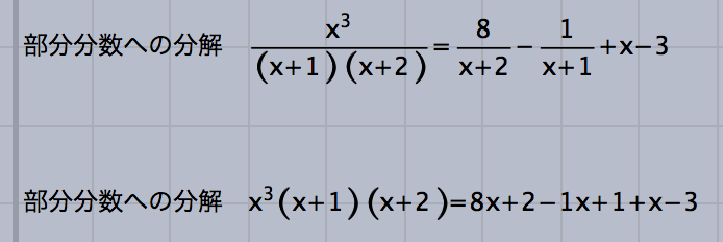
\includegraphics[bb=0 0 347.02 116.01 , width=8cm]{Fig/mxtex01.pdf}
        
\vspace{\baselineskip}
出力したTeX挿入図では次のようになる。

%\vspace{\baselineskip}
%%% fig.tex 2016-4-25 8:55
%%% fig.sce 2016-4-25 8:55
{\unitlength=8mm%
\begin{picture}%
(  10.22000,   3.87000)(  -0.61000,   2.03000)%
\special{pn 8}%
%
\settowidth{\Width}{Decomposition into partial fractions}\setlength{\Width}{0\Width}%
\settoheight{\Height}{Decomposition into partial fractions}\settodepth{\Depth}{Decomposition into partial fractions}\setlength{\Height}{-0.5\Height}\setlength{\Depth}{0.5\Depth}\addtolength{\Height}{\Depth}%
\put(0.0500,5.0000){\hspace*{\Width}\raisebox{\Height}{Decomposition into partial fractions}}%
%
%
\settowidth{\Width}{$\dfrac{x^3}{\left(x+1\right)\,\left(x+2\right)}=\dfrac{8}{x+2}-\dfrac{1}{x+1}+x-3$}\setlength{\Width}{0\Width}%
\settoheight{\Height}{$\dfrac{x^3}{\left(x+1\right)\,\left(x+2\right)}=\dfrac{8}{x+2}-\dfrac{1}{x+1}+x-3$}\settodepth{\Depth}{$\dfrac{x^3}{\left(x+1\right)\,\left(x+2\right)}=\dfrac{8}{x+2}-\dfrac{1}{x+1}+x-3$}\setlength{\Height}{-0.5\Height}\setlength{\Depth}{0.5\Depth}\addtolength{\Height}{\Depth}%
\put(0.0500,3.5000){\hspace*{\Width}\raisebox{\Height}{$\dfrac{x^3}{\left(x+1\right)\,\left(x+2\right)}=\dfrac{8}{x+2}-\dfrac{1}{x+1}+x-3$}}%
%
%
\end{picture}}% 

なお,文字列を置換するのに,\verb|Assign(form,["frac","dfrac"])| ではなく,

Cindyscriptの文字列の関数 replace を用いて,

\hspace{10mm} \verb|dform=replace(form,"frac","dfrac");| 
      
としてもよい。

%\vspace{10mm}

\vspace{\baselineskip}
【例】2次関数のグラフを表示し,$x$軸との交点の$x$座標を表示する。

\begin{layer}{150}{0}
\putnotese{70}{50}{ %%% fig.tex 2016-4-25 11:28
%%% fig.sce 2016-4-25 11:28
{\unitlength=8mm%
\begin{picture}%
(   7.07000,   5.60000)(  -3.07000,  -3.60000)%
\special{pn 8}%
%
\special{pa -564 -630}\special{pa -522 -440}\special{pa -477 -255}\special{pa -433 -82}%
\special{pa -388 79}\special{pa -343 227}\special{pa -299 362}\special{pa -254 485}%
\special{pa -210 595}\special{pa -165 693}\special{pa -121 778}\special{pa -76 850}%
\special{pa -32 910}\special{pa 13 957}\special{pa 57 992}\special{pa 102 1014}\special{pa 146 1023}%
\special{pa 191 1020}\special{pa 236 1004}\special{pa 280 976}\special{pa 325 935}%
\special{pa 369 881}\special{pa 414 815}\special{pa 458 736}\special{pa 503 645}\special{pa 547 541}%
\special{pa 592 425}\special{pa 636 296}\special{pa 681 154}\special{pa 725 0}\special{pa 770 -167}%
\special{pa 814 -347}\special{pa 859 -539}\special{pa 879 -630}%
\special{fp}%
\settowidth{\Width}{$\frac{1-\sqrt{13}}{2}$}\setlength{\Width}{0\Width}%
\settoheight{\Height}{$\frac{1-\sqrt{13}}{2}$}\settodepth{\Depth}{$\frac{1-\sqrt{13}}{2}$}\setlength{\Height}{-0.5\Height}\setlength{\Depth}{0.5\Depth}\addtolength{\Height}{\Depth}%
\put(-1.9500,-0.5000){\hspace*{\Width}\raisebox{\Height}{$\frac{1-\sqrt{13}}{2}$}}%
%
%
\settowidth{\Width}{$\frac{\sqrt{13}+1}{2}$}\setlength{\Width}{0\Width}%
\settoheight{\Height}{$\frac{\sqrt{13}+1}{2}$}\settodepth{\Depth}{$\frac{\sqrt{13}+1}{2}$}\setlength{\Height}{-0.5\Height}\setlength{\Depth}{0.5\Depth}\addtolength{\Height}{\Depth}%
\put(2.0500,-0.5000){\hspace*{\Width}\raisebox{\Height}{$\frac{\sqrt{13}+1}{2}$}}%
%
%
\special{pn 8}%
\special{pa -967 0}\special{pa 1228 0}%
\special{fp}%
\special{pn 8}%
\special{pa 1185 24}\special{pa 1260 0}\special{pa 1185 -24}\special{pa 1185 0}\special{pa 1185 24}%
\special{sh 1}\special{ip}%
\special{pn 1}%
\special{pa 1185 24}\special{pa 1260 0}\special{pa 1185 -24}\special{pa 1185 0}\special{pa 1185 24}%
\special{pa 1260 0}%
\special{fp}%
\special{pn 8}%
\special{pn 8}%
\special{pa 0 1134}\special{pa 0 -598}%
\special{fp}%
\special{pn 8}%
\special{pa 24 -555}\special{pa 0 -630}\special{pa -24 -555}\special{pa 0 -555}\special{pa 24 -555}%
\special{sh 1}\special{ip}%
\special{pn 1}%
\special{pa 24 -555}\special{pa 0 -630}\special{pa -24 -555}\special{pa 0 -555}\special{pa 24 -555}%
\special{pa 0 -630}%
\special{fp}%
\special{pn 8}%
\settowidth{\Width}{$x$}\setlength{\Width}{0\Width}%
\settoheight{\Height}{$x$}\settodepth{\Depth}{$x$}\setlength{\Height}{-0.5\Height}\setlength{\Depth}{0.5\Depth}\addtolength{\Height}{\Depth}%
\put(4.0500,0.0000){\hspace*{\Width}\raisebox{\Height}{$x$}}%
%
%
\settowidth{\Width}{$y$}\setlength{\Width}{-0.5\Width}%
\settoheight{\Height}{$y$}\settodepth{\Depth}{$y$}\setlength{\Height}{\Depth}%
\put(0.0000,2.0500){\hspace*{\Width}\raisebox{\Height}{$y$}}%
%
%
\settowidth{\Width}{O}\setlength{\Width}{-1\Width}%
\settoheight{\Height}{O}\settodepth{\Depth}{O}\setlength{\Height}{-\Height}%
\put(-0.0500,-0.0500){\hspace*{\Width}\raisebox{\Height}{O}}%
%
%
\end{picture}}%}
\end{layer}
\begin{verbatim}
    fx="x^2-x-3";
    cmdL=[
      "ans:solve",[fx,"x"],
      "ans",[]
    ];
    CalcbyM("ans",cmdL);
    p1=indexof(ans,"[");
    p2=indexof(ans,",");
    p3=indexof(ans,"]");
    s1=substring(ans,p1,p2-1);
    s2=substring(ans,p2,p3-1);
    s1=replace(s1,"x =","");
    s2=replace(s2,"x =","");
    Mxtex("1",s1);
    Mxtex("2",s2);
    Plotdata("1",fx,"x");
    Expr([-2,-0.5],"e",tx1);
    Expr([2,-0.5],"e",tx2);
\end{verbatim}

ここで,\verb|CalcbyM("ans",cmdL);| で得られるansは,次のような文字列である。
  
        \verb|"[x = -(sqrt(13)-1)/2,x = (sqrt(13)+1)/2] "|
        
そこで,ここから2つの式だけを抽出する作業を行ったのち,Mxtex() でTeXの式を得ている。

さらに応用として,点AをCinderellaの作図ツールで作図し,
\begin{verbatim}
    if(A.y<0,
      fx="(x-"+text(A.x)+")^2"+guess(A.y),
      fx="(x-"+text(A.x)+")^2+"+guess(A.y);
    );
\end{verbatim}
とすると,点Aを頂点とする放物線と軸との交点の座標が描かれる。Maximaとのデータのやり取りをするためのタイムラグがあるが,インタラクティブに放物線の位置を変えることができる。

\vspace{\baselineskip}
<参考>

  2次関数のような簡単な関数であれば,Cindyscriptの roots() 関数を用いて2次方程式が解けるので,次のスクリプトでほぼ同じ動作をするものを作ることができる。「ほぼ」というのは点Aの位置によっては,guess()で解釈しきれないことがあるためである。Maximaを使えば数式処理で解を求めるので,Aがどこにあってもきれいに表示できる。
\begin{verbatim}
    fx="x^2-2*A.x*x+A.x^2+A.y";
    cf=[A.x^2+A.y,-2*A.x,1];
    sol=roots(cf);
    s1=guess(sol_2);
    s2=guess(sol_1);
    Mxtex("1",s1);
    Mxtex("2",s2);
    Plotdata("1",fx,"x");
    Expr([-2,-0.5],"e",tx1);
    Expr([2,-0.5],"e",tx2);
\end{verbatim}

\end{description}

\begin{flushright}  \hyperlink{functionlist}{$\Rightarrow$関数一覧}\end{flushright}
\newpage


%  Risa/Asirとの連携  ==================================
\subsection{Risa/Asirとの連携}

\begin{description}

\hypertarget{calcbyA}{}
\item[関数]  CalcbyA(name,コマンド,option)
\item[機能]  Risa/Asirのスクリプトを実行する
\item[説明]  第2引数はRisa/Asirで実行するコマンド。

  コマンドと引数リストの繰り返しからなるリスト(例えばcmdL)を作って,一度に実行する。
  
  戻り値はない。(未定義値)  結果は,コマンドリストの最後に記述した変数(引数は空リスト)の値がname で指定された変数に代入される。複数の結果を戻すときは,:: で区切って記述するとリストにして代入される。
  

\vspace{\baselineskip}
\hypertarget{asirfun}{}
\item[関数]  Asirfun(name,式,リスト,option)
\item[機能]  Risa/Asirの関数を実行する
\item[説明]  第2引数の「式」はRisa/Asirの関数名。第3引数のリストは関数に渡す引数のリスト。

戻り値は,第1引数の式に1つでも文字があると文字列となる。すべて数字(+,-, . を含む)の場合は
16桁以下であれば数,それ以上の場合は文字列となる。また,戻り値は,変数 asname にも代入される。

オプションに "Disp=no" をつけると,結果をコンソールに表示しない。


\end{description}
\begin{flushright}  \hyperlink{functionlist}{$\Rightarrow$関数一覧}\end{flushright}

\newpage
%  FriCASとの連携  ==================================
\subsection{FriCAS(Axiom)との連携}

\begin{description}

\hypertarget{calcbyF}{}
\item[関数]  CalcbyF(name,コマンド,option)
\item[機能]  FriCASのスクリプトを実行する
\item[説明]  第2引数はFriCASで実行するコマンド。

コマンドと引数リストの繰り返しからなるリスト(例えばcmdL)を作って,一度に実行する。

戻り値はない。(未定義値)  結果は,コマンドリストの最後に記述した変数(引数は空リスト)の値がname で指定された変数に代入される。複数の結果を戻すときは,:: で区切って記述するとリストにして代入される。


\vspace{\baselineskip}
\hypertarget{frfun}{}
\item[関数]  Frfun(name,式,リスト,option)
\item[機能]  FriCASの関数を実行する
\item[説明]  第2引数の「式」はFriCASの関数名。第3引数のリストは関数に渡す引数のリスト。

戻り値は,第1引数の式に1つでも文字があると文字列となる。すべて数字(+,-, . を含む)の場合は
16桁以下であれば数,それ以上の場合は文字列となる。また,戻り値は,変数 friname にも代入される。

オプションに "Disp=no" をつけると,結果をコンソールに表示しない。


\end{description}
\begin{flushright}  \hyperlink{functionlist}{$\Rightarrow$関数一覧}\end{flushright}

\newpage

%  MeshLabとの連携  ==================================
\subsection{MeshLabとの連携}

MeshLabは,3Dデータ(objデータなど)を読み込んでレイトレーシングで表示・編集するソフトウェアである。レイトレーシングで3Dグラフィクスを描くには,Cinderellaと親和性の高い Cindy3D を利用するのがよいが,MeshLabを使うメリットは3Dプリンタ用のSTLファイルを出力できることである。また,\ketcindy で描いた3Dの図がレイトレーシングでどのようになるのかを見ることも比較的簡単にできる。

MeshLabとの連携は,\ketcindy から Obj 形式のデータを書き出すことで行う。Mkobj**() 関数でデータを作り,Mkviewobj() 関数でMeshLabを呼び出して表示を行う。
  
なお,Mkviewobj() 関数でMeshLabを呼び出して表示を行う場合,これをDrawスロットに書くと頻繁に呼び出しが行われるため非効率となる。そこで,if(1==0,・・・) で・・・の部分にMeshLabの呼び出し関係のスクリプトを書いて,実際に呼び出すときに if(1==1,・・・)とする方法と,呼び出し関係のスクリプトを関数化してボタンに割り当てる方法がある。ketcindyパッケージに含まれる sample にボタンをつけたものがある。
  
  なお,3Dであるので,Initialization スロットに
  
    \verb|Ketinit();|
    \verb|Ketinit3d();|
を記述しておく。

\begin{description}

\hypertarget{mkobjcmd}{}
\item[関数]  Mkobjcmd(name,式,option)
\item[機能]  厚みを持たない曲面のobjファイルのためのコマンドを作成する
\item[説明]  オプションは [分割数1,分割数2,表側の方向の指定]

表側の方向は,変数に対して,右手系の方向が"+"

作成されるデータは"oc"+name のファイル名の obj データである。この名称は,Mkviewobj() で用いる。(以下,Mkobj**()関数では同様)

\vspace{\baselineskip}
【例】:サドル面
\begin{verbatim}
    fd=[ "z=x^2-y^2", "x=[-1,1]","y=[-1,1]"," "];
    Sf3data("1",fd);
    Windispg();
    Mkobjcmd("1",fd,[40,40,"-"]); 
    Meshlab():=(
      Mkviewobj("saddle",oc1, ["m","v"]); 
    );
\end{verbatim}
このうち,\verb|Sf3data("1",fd); | はCinderellaの画面に表示するためであって,なくてもよい。

次図で,左が option + の場合,右が - の場合である。

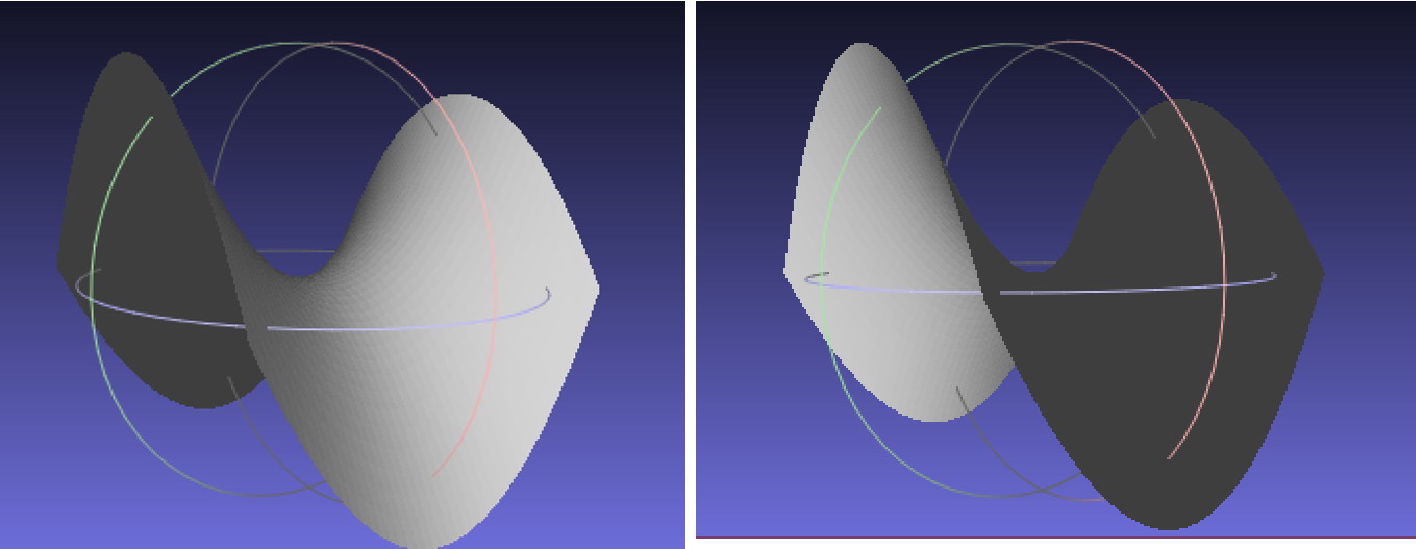
\includegraphics[bb=0 0 679.53 263.51 , width=12cm]{Fig/meshlab01.pdf}
\vspace{\baselineskip}
\begin{flushright}  \hyperlink{functionlist}{$\Rightarrow$関数一覧}\end{flushright}

\vspace{\baselineskip}
\hypertarget{mkobjcrvcmd}{}
\item[関数]  Mkobjcrvcmd(name,PD,option)
\item[機能]  空間曲線(直線)のobjファイルのためのコマンドを作成
\item[説明]  オプションは [太さ,断面の形状(正多角形)の辺の数,断面の正面]

曲線は紐のようなもので表す。その断面は正多角形で, 初期設定は正6角形である。断面の正面は"xy","yz","zx"のいずれかで指定する。太くなった時に形状の差が現れる。

例  太さ0.03で螺旋を描く
\begin{verbatim}
  Spacecurve("1","[(6*pi-t)/(6*pi)*cos(t),(6*pi-t)/(6*pi)*sin(t),0.1*t]",
    "t=[0,6*pi]",["Num=200"]);
  Windispg();
  Mkobjcrvcmd("1","sc3d1",[0.03]);
  Meshlab():=(
  Mkviewobj("spiral",oc1,["m","v"]); 
  );
\end{verbatim}

\verb|  Mkobjcrvcmd("1","sc3d1",[0.1,8,"yz"]);| としたのが下図右。
  
 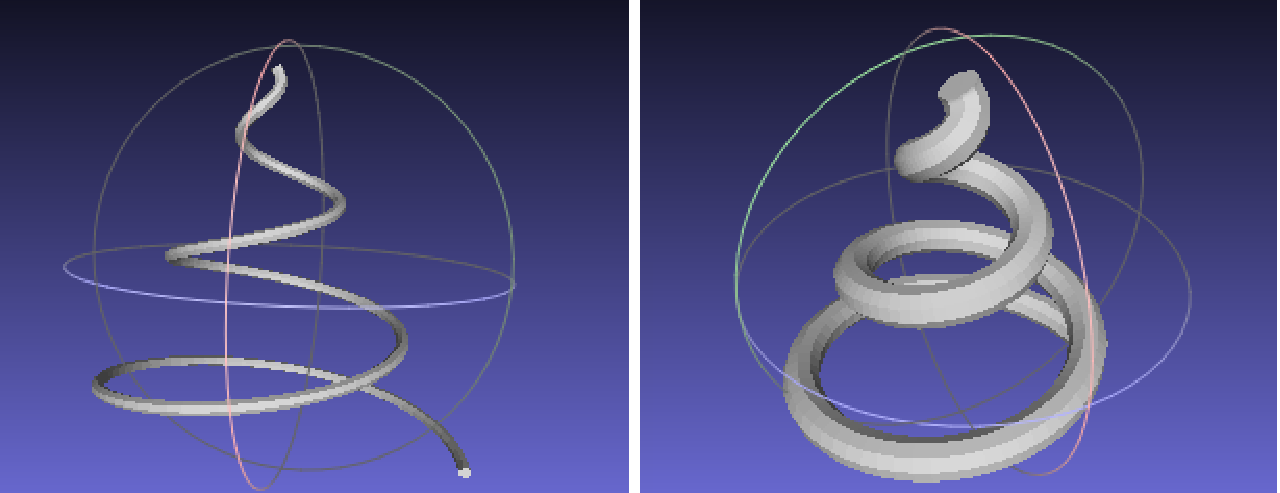
\includegraphics[bb=0 0 614.53 236.51 , width=12cm]{Fig/meshlab02.pdf}
  
\begin{flushright}  \hyperlink{functionlist}{$\Rightarrow$関数一覧}\end{flushright}

\vspace{\baselineskip}
\hypertarget{mkobjnrm}{}
\item[関数]  Mkobjnrm(name,式)
\item[機能]  法線ベクトルのデータを作成
\item[説明]  式は曲面を表す式。これに対し,法線ベクトルを表す式を求める。

\vspace{\baselineskip}
\hypertarget{mkobjplatecmd}{}
\item[関数]  Mkobjplatecmd(name,面データ,options)
\item[機能]  面を描く
\item[説明]  面データを渡して面を描く。

options は,面の厚みの指定。厚みは中心線に対し,両側につけることができる。

たとえば,[0.05] はプラス側に 0.05 の厚み,[0.05,-0.04] はマイナス側にも0.04の厚みをつける。

\vspace{\baselineskip}
【例】三角形のプレートを描く

\begin{layer}{150}{0}
\putnotese{80}{15}{ 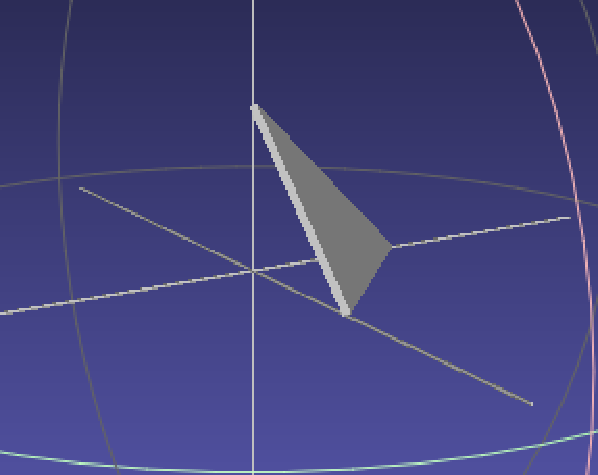
\includegraphics[bb=0 0 287.01 228.01 , width=3cm]{Fig/meshlab03.pdf} }
\end{layer}
\begin{verbatim}
  Xyzax3data("","x=[-5,5]","y=[-5,5]","z=[-5,5]");
  p1=[2,0,0];
  p2=[0,2,0];
  p3=[0,0,2];
  plane=[[p1,p2,p3],[[1,2,3]]];
  Mkobjplatecmd("1",plane,[0.05]);
  Mkobjcrvcmd("2","ax3d");
  Mkviewobj("plane",Concatcmd([oc1,oc2]),["m","v"]); 
  \end{verbatim}

\vspace{\baselineskip}
\hypertarget{mkobjpolycmd}{}
\item[関数]  Mkobjpolycmd(name,PD,options)
\item[機能]  多面体を描く
\item[説明]  VertexEdgeFace() の戻り値を PDとして渡して多面体を描く。

\vspace{\baselineskip}
\hypertarget{mkobjsymbcmd}{}
\item[関数]  Mkobjsymbcmd(PD, 実数,実数,ベクトル, ベクトル)
\item[機能]  文字等のobjデータのためのコマンドを作成
\item[説明]  引数のPDを描く。第2引数は大きさ,第3引数は回転角,第4引数は正面方向のベクトル,第5引数はPDの中心の位置。

PDは,平面の描画コマンドによるプロットデータが使える。また,PD に半角アルファベットを文字として与えることができる。この場合,文字は n,p,q,r,t,x,y,z で,該当するフォントが data フォルダの fontF フォルダに用意されている。この中にないフォントは使えない。

\vspace{\baselineskip}
\hypertarget{mkobjthickcmd}{}
\item[関数]  Mkobjthickcmd(name,式)
\item[機能]  厚みを持つ曲面のobjファイルのためのコマンドを作成
\item[説明]  オプションは [分割数1,分割数2,厚み,表側の方向の指定,条件]
表側の方向は,変数に対して,右手系の方向が"+"。厚みを持つため,nsew のそれぞれについて,
"+n+s-e-w" のように指定する。

条件として,\verb|"Assume(R>0)"| をつけると,Rが0以下になるための不具合を回避できる。

また,"ratsimp" をつけると有理関数について,"trigsimp"をつけると三角関数について,処理を速くすることができる。

なお,この関数はMaximaを使うので,Maximaをインストールしていることが前提。

\vspace{\baselineskip}
【例】回転放物線

\begin{layer}{150}{0}
\putnotese{70}{0}{ 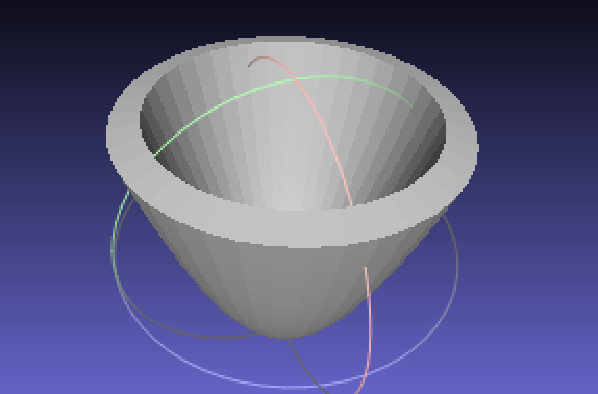
\includegraphics[bb=0 0 287.01 189.01 , width=4cm]{Fig/meshlab06.pdf}}
\end{layer}
\begin{verbatim}
  fd=[
  "z=(x^2+y^2)",
  "x=R*cos(T)","y=R*sin(T)",
  "R=[0,2]","T=[0,2*pi]","e"
  ];
  Mkobjthickcmd("1",fd,[40,40,0.2,"+n+s-e-w+","assume(R>0)"]);
  Mkviewobj("pala",oc1,["m","v","Wait=5"]); 
\end{verbatim}

%\begin{center}  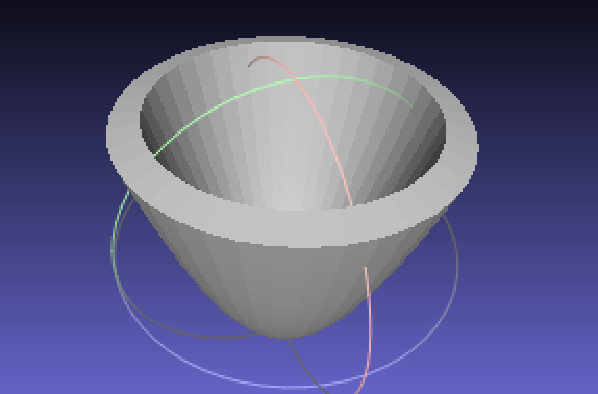
\includegraphics[bb=0 0 574 378 , width=5cm]{Fig/meshlab06.pdf}\end{center}

\vspace{\baselineskip}
\hypertarget{mkviewobj}{}
\item[関数]  Mkviewobj(name,PD, options)
\item[機能]  objファイルを作成。optionにより MeshLab を立ち上げて表示する。
\item[説明]  第2引数に複数のプロットデータを与えるときは,Concatcmd() により1つにまとめる。
オプションは 
\begin{tabbing}
12345678901234567890\=\kill
  "m"または"make"  \> データを作る(指定しない場合もデータがなければ作る)\\
  "v"または"view"    \>MeshLabを立ち上げて表示する\\
  "W=n"            \>作成するための待ち時間。n秒。これを過ぎると終了する\\
  "Unit=mm"        \>Setunitlen()と連動して3Dプリンタの数値の単位をmmで指定する\\
    \>3Dプリンターがインチで認識する場合は "Unit=in" とする。\\
\end{tabbing}


\end{description}
\begin{flushright}  \hyperlink{functionlist}{$\Rightarrow$関数一覧}\end{flushright}

\newpage
%  表計算ソフトとの連携  ==================================
\subsection{表計算ソフトとの連携}
表計算ソフトでは,複数のセルを選択してコピー(Windowsでは Crtl+ C ,Macでは Command+C)すると,セルの内容はtab区切りのテキストデータとしてクリップボードにコピーされる。これをCindyscriptエディタにペーストすることで表計算ソフトのデータを\ketcindy で利用できる。逆に,Cindyscriptのコンソールへの出力を表計算ソフトのシートにコピーすることもできる。

また,表計算ソフトから書き出したCSVファイルについても同様にしてCSV形式のデータを扱うことができる。

\begin{description}
\hypertarget{tab2list}{}
\item[関数]  Tab2list(str,option)
\item[機能]  str の内容をリストに変換する
\item[説明]  tabやコンマ区切りになっている文字列 str をリストに変換する。

 optionは,次の通り。
 
 Blank=a  :NULLのセルをaに置き換える。
 
Sep=b    :セパレータ(区切り文字)を b とする。 初期設定は tabコード

次のような手順で表計算ソフトやCSVファイルからデータを\ketcindy に移すことができる。

\vspace{\baselineskip}
(1) Cindyscriptエディタで,適当な文字変数を用意する。

  たとえば,data="";
  
\vspace{\baselineskip}
\hspace{10mm} 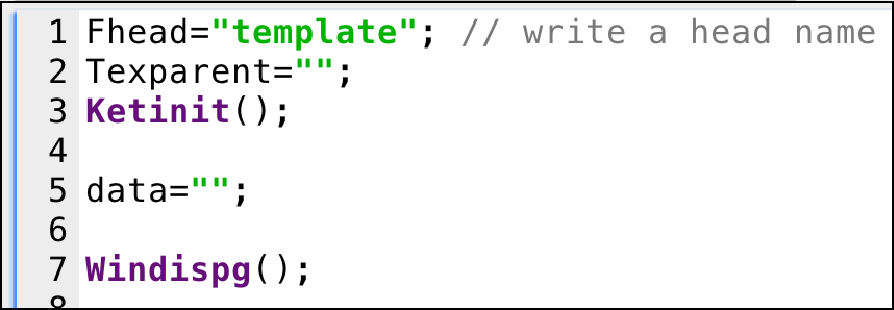
\includegraphics[bb=0 0 429.02 149.01 , width=7cm]{Fig/tab2list02.pdf}

\vspace{\baselineskip}
(2) 表計算ソフトで,適当な範囲を指定しクリップボードにコピーする。

  Windowsなら Ctrl+C,Macなら Command+C
  
\vspace{\baselineskip}
\hspace{10mm} 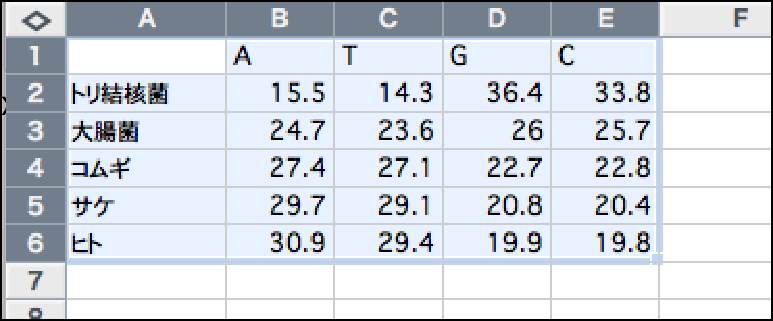
\includegraphics[bb=0 0 371.02 154 , width=7cm]{Fig/tab2list01.pdf}

\vspace{\baselineskip}
(3) data=""; のダブルクウォートの間にペーストする。

最後の行は右図のように," の前で改行されていてもよい。

\vspace{\baselineskip}
\hspace{10mm} 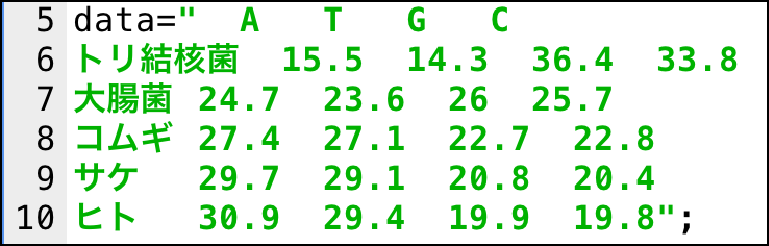
\includegraphics[bb=0 0 369.02 118.01 , width=6cm]{Fig/tab2list00.pdf}

\hspace{10mm} 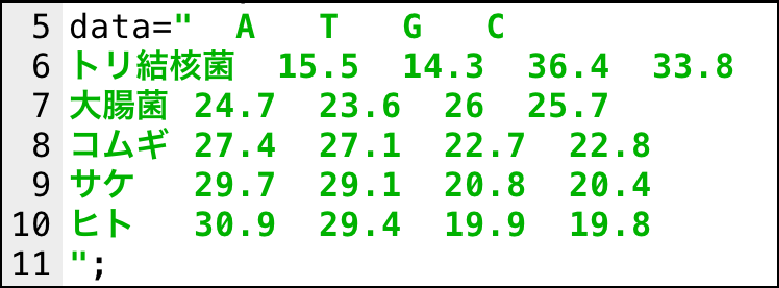
\includegraphics[bb=0 0 374.02 138.01 , width=6cm]{Fig/tab2list001.pdf}
    
\vspace{\baselineskip}
(4) この文字変数 data に対し,Tab2list(data) を実行すると,行列を表すリストが返される。

これを適当な変数に代入し,作表コマンドで表にするなど,目的に応じて利用する。
  
数値だけなら行列として計算もできる。

\vspace{\baselineskip} 
\hspace{10mm} 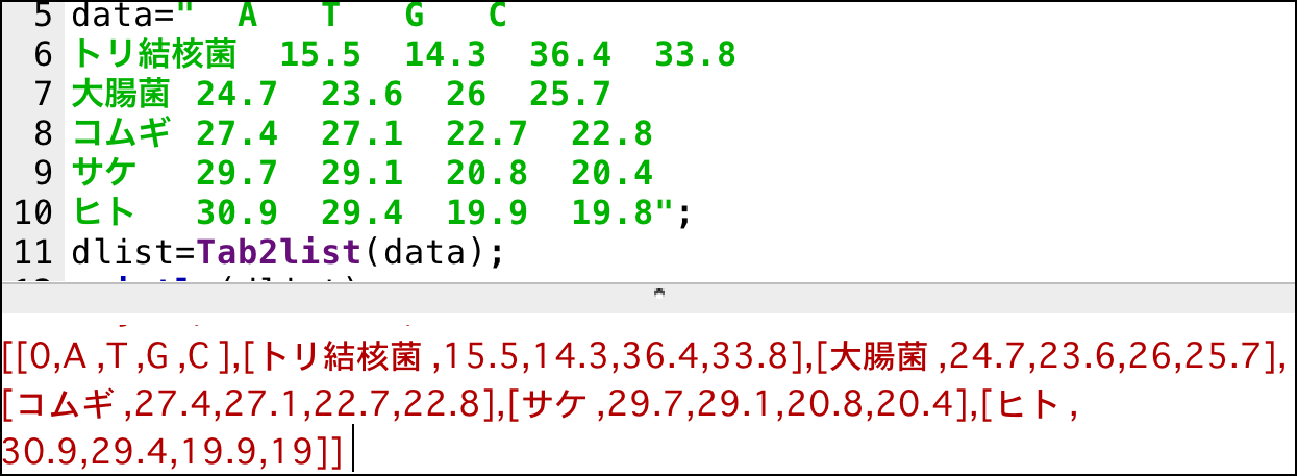
\includegraphics[bb=0 0 622.53 228.51 , width=10cm]{Fig/tab2list03.pdf}

\vspace{\baselineskip}
  空文字のセル(NULL)が含まれる場合, 初期設定ではそのまま空文字になるが,アンケート処理などで無回答を0にしたいような場合は
  
\hspace{10mm}\verb|dlist=Tab2list(data,["Blank=0"];|

とする。
 
 CSVファイルからCSV形式(コンマ区切り)のデータをコピーした場合は
 
\hspace{10mm}  \verb|dlist=Tab2list(data,["Sep=,"];|
  
とする。
 
なお,文字列をセパレータで区切ってリスト化するCindyscriptの関数に tokenize()がある。上の例で,

\hspace{10mm} \verb|dlist=tokenize(data,[unicode("000a"),unicode("0009")]);|
     
とすると,改行コード(000a)とtabコード(0009)で切り分けてリスト化する。このとき,リストの各要素はつぎのようになる。

文字列→文字列
  
数値形式の文字→実数    【例】 14 → 整数14    12.3 → 実数12.3

計算式の形  →  文字列  【例】 437-0023 →  437-0023 (文字列)

これに対し,Tab2list()では,計算式の形の文字列は数値と見なして計算結果を取得する。

\vspace{\baselineskip}
【例】 437-0023 →  414 (数値)

したがって,郵便番号や日付(28/12/5)のようなものは計算されてしまうので,tokenize() を用いるのがよい。なお,tokenize()の場合,空行は空リストになるので,最後の行でダブルクウォートの前で改行されていると空リストが入る。


\vspace{\baselineskip}
\hypertarget{dispmat}{}
\item[関数]  Dispmat(list)
\item[機能]  リストを行列の形でtab区切りにしてコンソールに表示する。
\item[説明]  行列を表すリスト (たとえば dlist) を引数としてDispmat(dlist) を実行すると,コンソールに行列型で内容が表示される。

実際にはTAB区切りの文字列。(println としなくても直接コンソールに表示される)

これを表計算ソフトのシートにコピーする。

\vspace{\baselineskip}
\hspace{10mm} 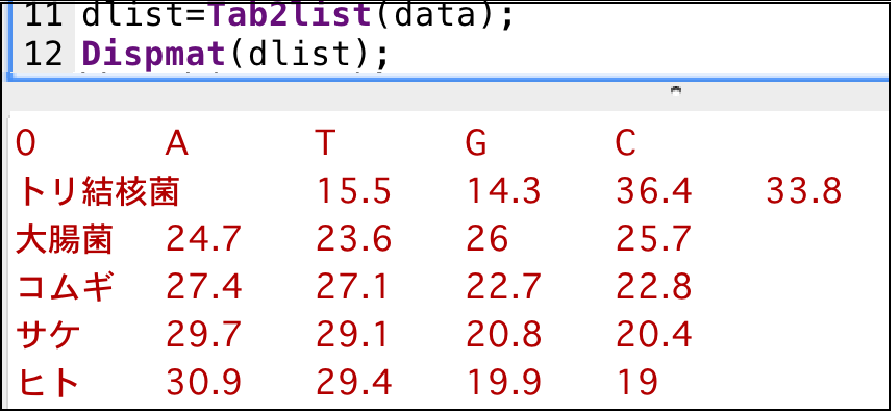
\includegraphics[bb=0 0 427.52 197.51 , width=7cm]{Fig/tab2list04.pdf}


\vspace{\baselineskip}
\hypertarget{writecsv}{}
\item[関数]  Writecsv(namelist, data, filename, option)
\item[機能]  data の内容をCSVファイルに出力する
\item[説明]  ベクトルまたは行列となっている data を、filenameのファイル名としてCSVファイルに書き出す。

optionは,次の通り。(省略できる)

Col=nn  :自然数nnで指定した列数のCSVファイルとして書き出す。
 
namelistは,CSVファイルの1行目に追加される項目名。省略すると"C1,C2,..."という項目名が付く。

 
なお,列数の指定を省略するとdataが行列の場合は、その列数をdataがベクトルの場合はnamelistの項目数を利用する。

\end{description}

\begin{flushright}  \hyperlink{functionlist}{$\Rightarrow$関数一覧}\end{flushright}

\newpage


%  アニメーション  ==================================
\section{アニメーションPDF}
\subsection{概要}
アニメーションのできるPDFを作る。

Cinderellaの作図機能とCindyscriptを用いてアニメーションができるが,PDFにすることでCinderellaがなくてもPDFビュアーがあればアニメーションを実行できるので,プレゼンテーションや教材の受け渡しなどに便利である。

次の画面は,samplesフォルダにある「s06animation」の「s0601cycloid」のものである。これをひな形として使うのがよい。

\vspace{\baselineskip}
    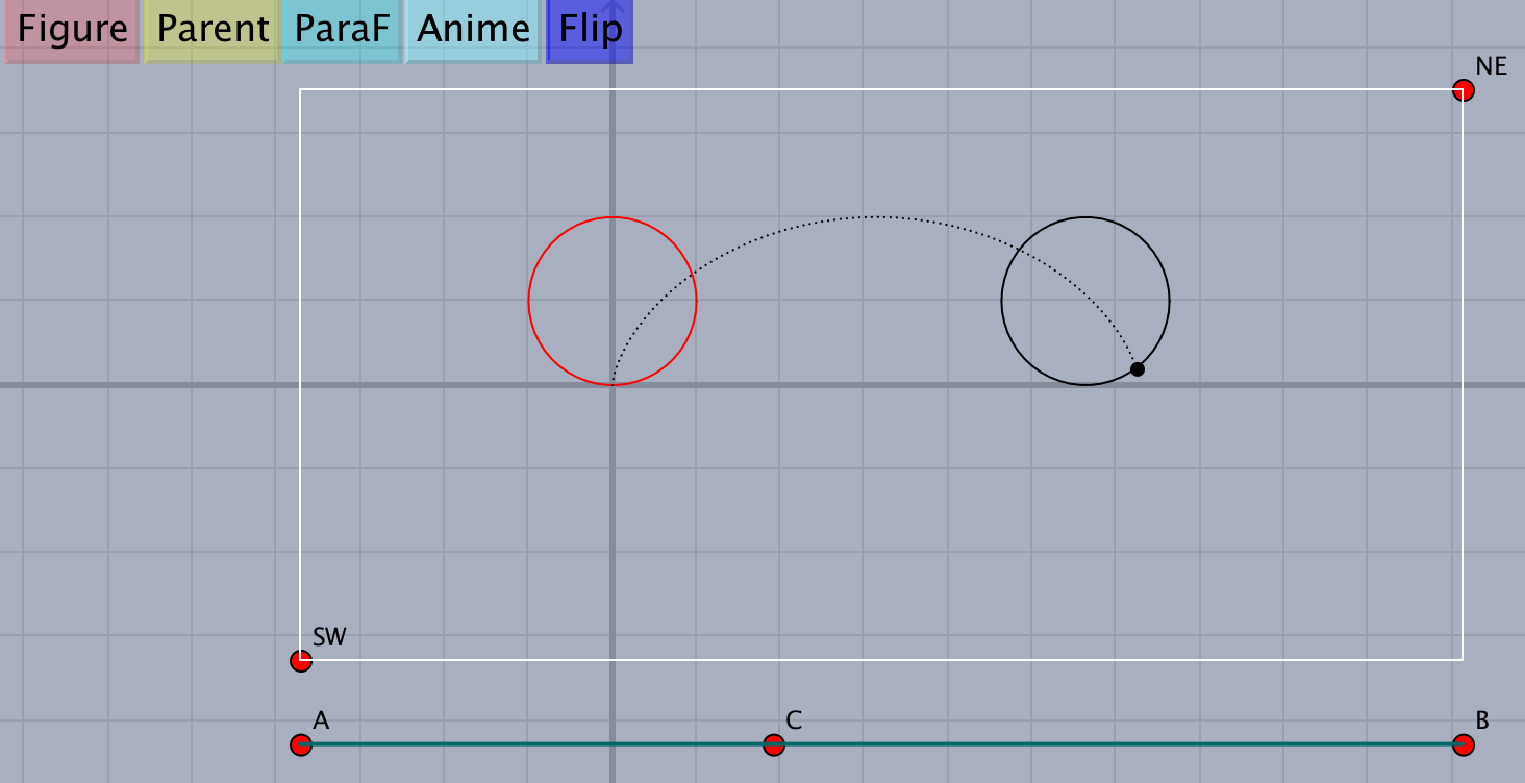
\includegraphics[bb=0 0 732.04 376.02 , width=12cm]{Fig/mvgaiyou01.pdf}

画面上方のボタンには,次のようなスクリプトが割り当てられている。

\begin{tabbing}
  12345678\=1234567897890123456\=\kill
  Figure  \>: Viewtex(); \>現在の画面のPDFデータを作る\\
  Parent   \>:複数のスクリプト    \>Figpdf() を使うときに使用する。\\
  ParaF \>: Parafolder(); \>アニメーションのデータを作る\\
  Anime  \>: Mkanimation(); \>アニメーションPDFを作る\\
  Flip   \>: Mkflipanime(); \>パラパラ動画PDFを作る
\end{tabbing}

アニメーションの作成は,フレームを定義する関数を作成し,Mkanimation() 関数を実行する(Animeボタン)。
%たとえば,Fhead が "hoge" の場合,TeX の文書には\\
%         \verb|\begin{center} \input{hogemoviefigs.tex}|\\
%で動画を挿入することができる。

%ただし,動画のできるPDFを作成するには,ドキュメントクラスと使用パッケージについて注意が必要である。

%ドキュメントクラスは,article または jarticle とする。jsarticle は使えない。

%パッケージは animate に dvipdfmx オプションをつける。\\
%            \verb|\usepackage[dvipdfmx]{animate}|

なお,アニメーションPDFでアニメーションを行うにはAdobe Acrobat Reader など,アニメーションに対応したPDFリーダーが必要である。WindowsのSumatraPDF,Macの プレビューでは動かない。

Flipボタンを押すと,フレームに分割したPDFが生成されて表示される。

\subsection{関数}
\begin{description}

\hypertarget{setpara}{}
\item[関数]  Setpara(fname,funcstr,range,options1,options2)
\item[機能]  アニメーションの設定をする
\item[説明]  fname は出力するファイル名,funcstrは動画関数名,rangeは範囲

options1 はアニメーションのデータを作るための設定。
\begin{tabbing}
1234567890123\=90123456789012345678\=\kill
m/r    \> データの作成 / 既存データがある場合の読み込み( 初期設定は r )\\
Div=n  \> フレーム数。初期値は25。
\end{tabbing}
options2 はアニメーションについての設定で,次の通り。
\begin{tabbing}
1234567890123\=90123456789012345678\=\kill
Frate=n  \>1秒間のフレーム数。初期値は20。 \\
Title=str  \> タイトル。\\
Scale=n  \> 図の大きさの拡大率 \\
opA  \> animate.sty のためのオプション。 \\
  \> loop:loopする,controls:ボタンを表示,buttonsize:ボタンのサイズ\\
  \> step:コマ送りモード\\
  \>  初期設定は  loop,controls,buttonsize=3mm\\
  \> +をつけるとモードが追加される。たとえば \verb|"OpA=+step"| で\\
  \>  \verb|"OpA=[loop,controls,buttonsize=3mm,step]"| となる。
\end{tabbing}

\vspace{\baselineskip}
\item[関数] Parafolder(funcstr,fname,range,options)
\item[機能]  アニメーションのフレームデータを作成する
\item[説明]  funcstrは動画関数名,fname は出力するフォルダ名,rangeは範囲

作業フォルダ(fig)内に,フレームデータを格納した fname フォルダを作る。ひな形(s0601cycloid)にある ParaF ボタンに割り当てられており,通常はそのまま使えばよい。

\vspace{\baselineskip}
\item[関数]  Mkanimation(path,folder)
\item[機能]  アニメーションのPDFを作る
\item[説明]  作業フォルダ(fig)内に,フレームデータを格納した fname フォルダを作り,ここからアニメーションのPDFを作る。Setpara() で設定したファイル名を fname とすると,生成する TeX ファイルは,animatefname.tex (PDF作成のTeXファイル)と animfname.tex (動画データ)で,PDFの名称は,animatefname.pdf となる。

ひな形(s0601cycloid)にある Anime ボタンに割り当てられており,通常はあらためて設定せずそのまま使えばよい。

\vspace{\baselineskip}
\item[関数]  Mkflipanime(path,folder)
\item[機能]  パラパラ動画のPDFを作る
\item[説明]  作業フォルダ(fig)内に,フレームデータを格納した fname フォルダを作り,ここからパラパラ動画のPDFを作る。Setpara() で設定したファイル名を fname とすると,生成する TeX ファイルは,flipanimefname.tex (PDF作成のTeXファイル)で,PDFの名称は,flipanimefname.pdf となる。

ひな形にある Flip ボタンに割り当てられており,通常はあらためて設定せずそのまま使えばよい。

\end{description}

\begin{flushright}  \hyperlink{functionlist}{$\Rightarrow$関数一覧}\end{flushright}

\subsection{制作例}

%\begin{description}
\vspace{\baselineskip}
【例】定円上を動く点Pと,定点Aを結ぶ線分の中点をQとして動きを見る。
アニメーションを定義する関数は,時間を $t$ とすれば,時刻 $t$ における図(動くものだけ)を定義する。時刻は単なる媒介変数であるので,$t$ でなく $s$ などでもよい。

\begin{verbatim}
  Setax(["","","sw","","sw"]);
  Slider("A-C-B",[0,YMIN-1],[2*pi,YMIN-1]);
  Circledata("1",[[0,0],[0,2]]);
  mf(t):=(
    pt=2*[cos(t),sin(t)];
    mp=(pt+[4,0])/2;
    Listplot("1",[[4,0],pt]);
    Pointdata("1",[mp,pt],["Size=2"]);
    if(t==0,
      ptlist=[mp];
    ,
      ptlist=append(ptlist,mp);
    );
    Letter([[4,0],"s","A",pt,"en","P",mp,"ne","Q"]);
    Pointdata("2",ptlist,["Size=2","Color=red"]);
  );
  mf(C.x);
  Setpara("middle","mf(t)","t=[0,4*pi]");
\end{verbatim}

この例の場合,\verb|mf(C.x)| を実行するとスライダを動かすことでインタラクティブに軌跡を表示できる。
Cinderellaの画面は次のようになる。

\vspace{\baselineskip}
\hspace{20mm} 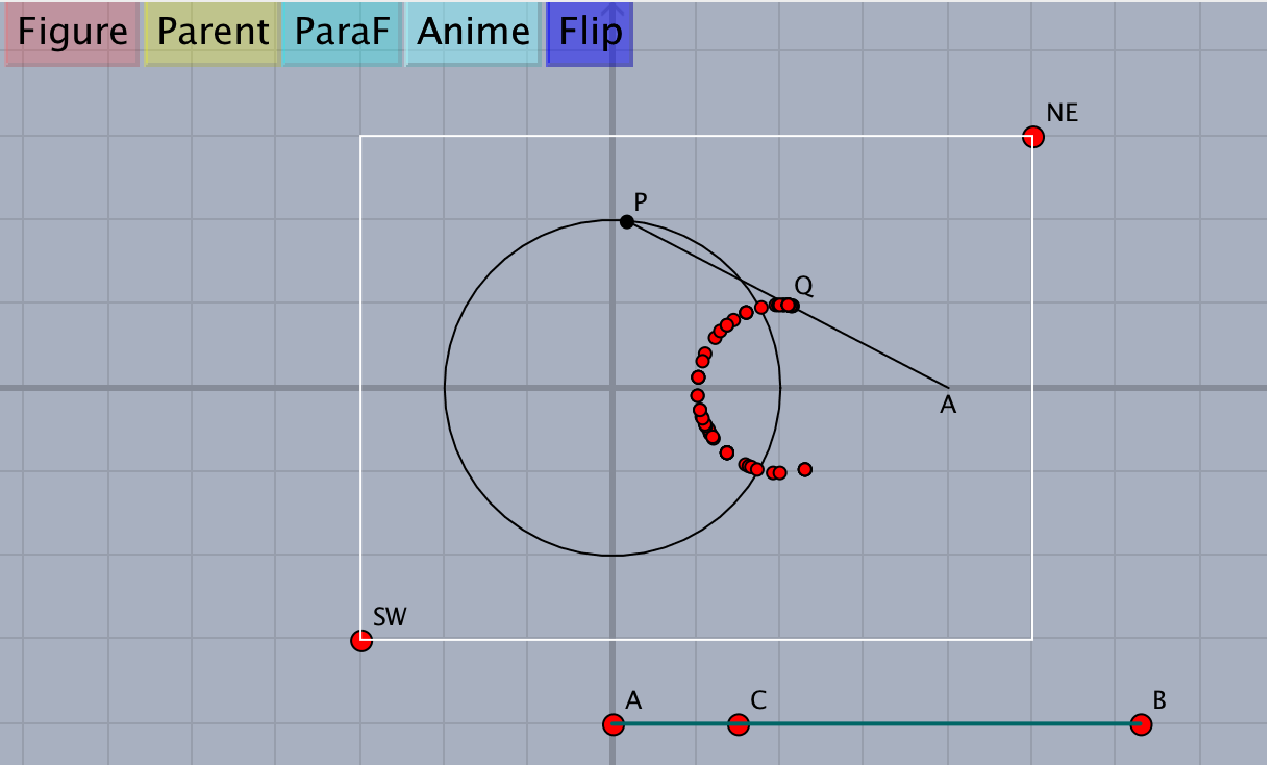
\includegraphics[bb=0.00 0.00 608.03 367.02,width=8cm]{Fig/moviedata01.pdf}

アニメーションを作成するときは \verb|//mf(C.x)| とコメントアウトしてから Anime ボタンをクリックする。次の図は,でき上がった animatemiddle.pdf の始めの画面である。

\hspace{30mm}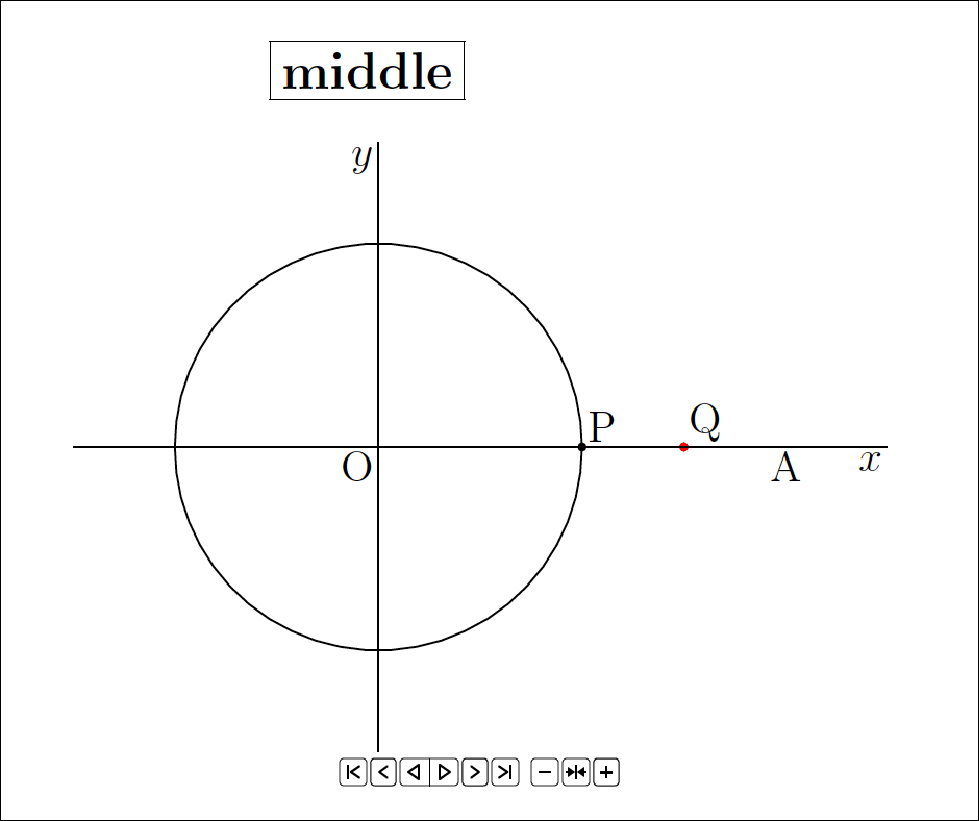
\includegraphics[bb=0.00 0.00 470.02 394.02,width=6cm]{Fig/moviedata02.pdf}

また,次のようにオプションを指定すると,5秒間のアニメーションとなる。

    \verb| Setpara("middle","mf(t)","t=[0,4*pi]",["Div=30"],["Frate=6"]);|
    
\verb|["Div=150"],["Frage=30"]|とすると,やはり5秒間のアニメーションとなるが,1秒間のフレーム数が多いため,なめらかな動きとなる。これは標準的なビデオのフレームレートである。ただし,ファイルサイズは約5倍となる。


\begin{flushright} \hyperlink{functionlist}{$\Rightarrow$関数一覧}\end{flushright}

%\end{description}

\newpage


%==================== Slide ===============
\section{\ketcindy スライド}
\subsection{概要と制作手順}
\ketcindy で作成した図とテキストを統合してプレゼンテーション用のスライドPDFを作成する。必要なファイルは,スライドの内容を記述したテキストファイル(ここではコンテンツファイルと呼ぶ)と,タイトルや図を作成し,コンテンツファイルと統合する \ketcindy のファイルである。この2つのファイルは,拡張子が txt と cdy で,ファイル名は同一とする。たとえば,コンテンツファイルを makeslide.txt , \ketcindy ファイルを makeslide.cdy としたときの,制作イメージを次の図に示す。

\hspace{10mm}%%% /Users/Hannya/Desktop/fig/makeslide.tex 
%%% Generator=makeslide.cdy 
{\unitlength=1cm%
\begin{picture}%
(10.5,7.5)(-6.5,-2)%
\special{pn 8}%
%
{%
\color[rgb]{0,0,0}%
\special{pa -1575  -787}\special{pa -1575  -906}\special{pa -1576  -918}\special{pa -1579  -930}%
\special{pa -1583  -941}\special{pa -1590  -952}\special{pa -1598  -961}\special{pa -1607  -969}%
\special{pa -1618  -976}\special{pa -1629  -980}\special{pa -1641  -983}\special{pa -1654  -984}%
\special{pa -1969  -984}\special{pa -2283  -984}\special{pa -2296  -983}\special{pa -2308  -980}%
\special{pa -2319  -976}\special{pa -2330  -969}\special{pa -2339  -961}\special{pa -2347  -952}%
\special{pa -2354  -941}\special{pa -2358  -930}\special{pa -2361  -918}\special{pa -2362  -906}%
\special{pa -2362  -787}\special{pa -2362  -669}\special{pa -2361  -657}\special{pa -2358  -645}%
\special{pa -2354  -634}\special{pa -2347  -623}\special{pa -2339  -614}\special{pa -2330  -606}%
\special{pa -2319  -599}\special{pa -2308  -594}\special{pa -2296  -592}\special{pa -2283  -591}%
\special{pa -1969  -591}\special{pa -1654  -591}\special{pa -1641  -592}\special{pa -1629  -594}%
\special{pa -1618  -599}\special{pa -1607  -606}\special{pa -1598  -614}\special{pa -1590  -623}%
\special{pa -1583  -634}\special{pa -1579  -645}\special{pa -1576  -657}\special{pa -1575  -669}%
\special{pa -1575  -787}%
\special{fp}%
}%
{%
\color[rgb]{0,0,0}%
\special{pa -1575  -197}\special{pa -1575  -315}\special{pa -1576  -327}\special{pa -1579  -339}%
\special{pa -1583  -351}\special{pa -1590  -361}\special{pa -1598  -371}\special{pa -1607  -379}%
\special{pa -1618  -385}\special{pa -1629  -390}\special{pa -1641  -393}\special{pa -1654  -394}%
\special{pa -1969  -394}\special{pa -2283  -394}\special{pa -2296  -393}\special{pa -2308  -390}%
\special{pa -2319  -385}\special{pa -2330  -379}\special{pa -2339  -371}\special{pa -2347  -361}%
\special{pa -2354  -351}\special{pa -2358  -339}\special{pa -2361  -327}\special{pa -2362  -315}%
\special{pa -2362  -197}\special{pa -2362   -79}\special{pa -2361   -66}\special{pa -2358   -54}%
\special{pa -2354   -43}\special{pa -2347   -32}\special{pa -2339   -23}\special{pa -2330   -15}%
\special{pa -2319    -9}\special{pa -2308    -4}\special{pa -2296    -1}\special{pa -2283    -0}%
\special{pa -1969    -0}\special{pa -1654    -0}\special{pa -1641    -1}\special{pa -1629    -4}%
\special{pa -1618    -9}\special{pa -1607   -15}\special{pa -1598   -23}\special{pa -1590   -32}%
\special{pa -1583   -43}\special{pa -1579   -54}\special{pa -1576   -66}\special{pa -1575   -79}%
\special{pa -1575  -197}%
\special{fp}%
}%
{%
\color[rgb]{0,0,0}%
\special{pa -1575   394}\special{pa -1575   276}\special{pa -1576   263}\special{pa -1579   251}%
\special{pa -1583   240}\special{pa -1590   229}\special{pa -1598   220}\special{pa -1607   212}%
\special{pa -1618   205}\special{pa -1629   201}\special{pa -1641   198}\special{pa -1654   197}%
\special{pa -1969   197}\special{pa -2283   197}\special{pa -2296   198}\special{pa -2308   201}%
\special{pa -2319   205}\special{pa -2330   212}\special{pa -2339   220}\special{pa -2347   229}%
\special{pa -2354   240}\special{pa -2358   251}\special{pa -2361   263}\special{pa -2362   276}%
\special{pa -2362   394}\special{pa -2362   512}\special{pa -2361   524}\special{pa -2358   536}%
\special{pa -2354   548}\special{pa -2347   558}\special{pa -2339   567}\special{pa -2330   576}%
\special{pa -2319   582}\special{pa -2308   587}\special{pa -2296   590}\special{pa -2283   591}%
\special{pa -1969   591}\special{pa -1654   591}\special{pa -1641   590}\special{pa -1629   587}%
\special{pa -1618   582}\special{pa -1607   576}\special{pa -1598   567}\special{pa -1590   558}%
\special{pa -1583   548}\special{pa -1579   536}\special{pa -1576   524}\special{pa -1575   512}%
\special{pa -1575   394}%
\special{fp}%
}%
{%
\color[rgb]{0,0,0}%
\special{pa  -114 -1189}\special{pa  -114 -1701}\special{pa  -115 -1713}\special{pa  -118 -1725}%
\special{pa  -123 -1737}\special{pa  -129 -1747}\special{pa  -137 -1756}\special{pa  -147 -1764}%
\special{pa  -157 -1771}\special{pa  -169 -1776}\special{pa  -181 -1779}\special{pa  -193 -1780}%
\special{pa  -508 -1780}\special{pa  -823 -1780}\special{pa  -835 -1779}\special{pa  -847 -1776}%
\special{pa  -859 -1771}\special{pa  -869 -1764}\special{pa  -879 -1756}\special{pa  -887 -1747}%
\special{pa  -893 -1737}\special{pa  -898 -1725}\special{pa  -901 -1713}\special{pa  -902 -1701}%
\special{pa  -902 -1189}\special{pa  -902  -677}\special{pa  -901  -665}\special{pa  -898  -653}%
\special{pa  -893  -641}\special{pa  -887  -631}\special{pa  -879  -621}\special{pa  -869  -613}%
\special{pa  -859  -607}\special{pa  -847  -602}\special{pa  -835  -599}\special{pa  -823  -598}%
\special{pa  -508  -598}\special{pa  -193  -598}\special{pa  -181  -599}\special{pa  -169  -602}%
\special{pa  -157  -607}\special{pa  -147  -613}\special{pa  -137  -621}\special{pa  -129  -631}%
\special{pa  -123  -641}\special{pa  -118  -653}\special{pa  -115  -665}\special{pa  -114  -677}%
\special{pa  -114 -1189}%
\special{fp}%
}%
{%
\color[rgb]{0,0,0}%
\special{pa    75    -0}\special{pa    75  -315}\special{pa    74  -327}\special{pa    71  -339}%
\special{pa    66  -351}\special{pa    60  -361}\special{pa    52  -371}\special{pa    42  -379}%
\special{pa    32  -385}\special{pa    20  -390}\special{pa     8  -393}\special{pa    -4  -394}%
\special{pa  -516  -394}\special{pa -1028  -394}\special{pa -1040  -393}\special{pa -1052  -390}%
\special{pa -1063  -385}\special{pa -1074  -379}\special{pa -1083  -371}\special{pa -1091  -361}%
\special{pa -1098  -351}\special{pa -1102  -339}\special{pa -1105  -327}\special{pa -1106  -315}%
\special{pa -1106    -0}\special{pa -1106   315}\special{pa -1105   327}\special{pa -1102   339}%
\special{pa -1098   351}\special{pa -1091   361}\special{pa -1083   371}\special{pa -1074   379}%
\special{pa -1063   385}\special{pa -1052   390}\special{pa -1040   393}\special{pa -1028   394}%
\special{pa  -516   394}\special{pa    -4   394}\special{pa     8   393}\special{pa    20   390}%
\special{pa    32   385}\special{pa    42   379}\special{pa    52   371}\special{pa    60   361}%
\special{pa    66   351}\special{pa    71   339}\special{pa    74   327}\special{pa    75   315}%
\special{pa    75    -0}%
\special{fp}%
}%
{%
\color[rgb]{0,0,0}%
\special{pa  1378    -0}\special{pa  1378  -315}\special{pa  1377  -327}\special{pa  1374  -339}%
\special{pa  1369  -351}\special{pa  1363  -361}\special{pa  1355  -371}\special{pa  1345  -379}%
\special{pa  1335  -385}\special{pa  1324  -390}\special{pa  1312  -393}\special{pa  1299  -394}%
\special{pa   984  -394}\special{pa   669  -394}\special{pa   657  -393}\special{pa   645  -390}%
\special{pa   634  -385}\special{pa   623  -379}\special{pa   614  -371}\special{pa   606  -361}%
\special{pa   599  -351}\special{pa   594  -339}\special{pa   592  -327}\special{pa   591  -315}%
\special{pa   591    -0}\special{pa   591   315}\special{pa   592   327}\special{pa   594   339}%
\special{pa   599   351}\special{pa   606   361}\special{pa   614   371}\special{pa   623   379}%
\special{pa   634   385}\special{pa   645   390}\special{pa   657   393}\special{pa   669   394}%
\special{pa   984   394}\special{pa  1299   394}\special{pa  1312   393}\special{pa  1324   390}%
\special{pa  1335   385}\special{pa  1345   379}\special{pa  1355   371}\special{pa  1363   361}%
\special{pa  1369   351}\special{pa  1374   339}\special{pa  1377   327}\special{pa  1378   315}%
\special{pa  1378    -0}%
\special{fp}%
}%
{%
\color[rgb]{0,0,0}%
\special{pa -1575  -787}\special{pa -1378  -787}\special{pa -1378   394}\special{pa -1575   394}%
\special{fp}%
}%
{%
\color[rgb]{0,0,0}%
\special{pa -1575  -197}\special{pa -1220  -197}%
\special{fp}%
}%
{%
\color[rgb]{0,0,0}%
}%
{%
\color[rgb]{0,0,0}%
\special{pa -1256 -173}\special{pa -1181 -197}\special{pa -1256 -221}\special{pa -1256 -197}%
\special{pa -1256 -173}\special{sh 1}\special{ip}%
\special{pn 1}%
\special{pa -1256  -173}\special{pa -1181  -197}\special{pa -1256  -221}\special{pa -1256  -197}%
\special{pa -1256  -173}\special{pa -1181  -197}%
\special{fp}%
\special{pn 8}%
}%
{%
\color[rgb]{0,0,0}%
\special{pa  -551  -407}\special{pa  -551  -564}%
\special{fp}%
}%
{%
\color[rgb]{0,0,0}%
}%
{%
\color[rgb]{0,0,0}%
\special{pa -526 -529}\special{pa -551 -604}\special{pa -575 -529}\special{pa -551 -529}%
\special{pa -526 -529}\special{sh 1}\special{ip}%
\special{pn 1}%
\special{pa  -526  -529}\special{pa  -551  -604}\special{pa  -575  -529}\special{pa  -551  -529}%
\special{pa  -526  -529}\special{pa  -551  -604}%
\special{fp}%
\special{pn 8}%
}%
{%
\color[rgb]{0,0,0}%
\special{pa  -472  -604}\special{pa  -472  -446}%
\special{fp}%
}%
{%
\color[rgb]{0,0,0}%
}%
{%
\color[rgb]{0,0,0}%
\special{pa -496 -482}\special{pa -472 -407}\special{pa -447 -482}\special{pa -472 -482}%
\special{pa -496 -482}\special{sh 1}\special{ip}%
\special{pn 1}%
\special{pa  -496  -482}\special{pa  -472  -407}\special{pa  -447  -482}\special{pa  -472  -482}%
\special{pa  -496  -482}\special{pa  -472  -407}%
\special{fp}%
\special{pn 8}%
}%
{%
\color[rgb]{0,0,0}%
\special{pa   160    80}\special{pa   160   -78}\special{pa   396   -78}\special{pa   396  -156}%
\special{pa   554     1}\special{pa   396   159}\special{pa   396    80}\special{pa   160    80}%
\special{fp}%
}%
{%
\color[rgb]{0,0,0}%
\settowidth{\Width}{fig1.tex}\setlength{\Width}{-0.5\Width}%
\settoheight{\Height}{fig1.tex}\settodepth{\Depth}{fig1.tex}\setlength{\Height}{-0.5\Height}\setlength{\Depth}{0.5\Depth}\addtolength{\Height}{\Depth}%
\put(-5.0000000,2.0000000){\hspace*{\Width}\raisebox{\Height}{fig1.tex}}%
%
}%
{%
\color[rgb]{0,0,0}%
\settowidth{\Width}{fig2.tex}\setlength{\Width}{-0.5\Width}%
\settoheight{\Height}{fig2.tex}\settodepth{\Depth}{fig2.tex}\setlength{\Height}{-0.5\Height}\setlength{\Depth}{0.5\Depth}\addtolength{\Height}{\Depth}%
\put(-5.0000000,0.5000000){\hspace*{\Width}\raisebox{\Height}{fig2.tex}}%
%
}%
{%
\color[rgb]{0,0,0}%
\settowidth{\Width}{movie.tex}\setlength{\Width}{-0.5\Width}%
\settoheight{\Height}{movie.tex}\settodepth{\Depth}{movie.tex}\setlength{\Height}{-0.5\Height}\setlength{\Depth}{0.5\Depth}\addtolength{\Height}{\Depth}%
\put(-5.0000000,-1.0000000){\hspace*{\Width}\raisebox{\Height}{movie.tex}}%
%
}%
{%
\color[rgb]{0,0,0}%
\settowidth{\Width}{makeslide.txt}\setlength{\Width}{-0.5\Width}%
\settoheight{\Height}{makeslide.txt}\settodepth{\Depth}{makeslide.txt}\setlength{\Height}{-0.5\Height}\setlength{\Depth}{0.5\Depth}\addtolength{\Height}{\Depth}%
\put(-1.4200000,4.7800000){\hspace*{\Width}\raisebox{\Height}{makeslide.txt}}%
%
}%
{%
\color[rgb]{0,0,0}%
\settowidth{\Width}{makeslide.cdy}\setlength{\Width}{-0.5\Width}%
\settoheight{\Height}{makeslide.cdy}\settodepth{\Depth}{makeslide.cdy}\setlength{\Height}{-0.5\Height}\setlength{\Depth}{0.5\Depth}\addtolength{\Height}{\Depth}%
\put(-1.3100000,0.0000000){\hspace*{\Width}\raisebox{\Height}{makeslide.cdy}}%
%
}%
{%
\color[rgb]{0,0,0}%
\settowidth{\Width}{Slide.pdf}\setlength{\Width}{-0.5\Width}%
\settoheight{\Height}{Slide.pdf}\settodepth{\Depth}{Slide.pdf}\setlength{\Height}{-0.5\Height}\setlength{\Depth}{0.5\Depth}\addtolength{\Height}{\Depth}%
\put(2.5000000,0.0000000){\hspace*{\Width}\raisebox{\Height}{Slide.pdf}}%
%
}%
{%
\color[rgb]{0,0,0}%
\settowidth{\Width}{Title}\setlength{\Width}{-0.5\Width}%
\settoheight{\Height}{Title}\settodepth{\Depth}{Title}\setlength{\Height}{-0.5\Height}\setlength{\Depth}{0.5\Depth}\addtolength{\Height}{\Depth}%
\put(-1.2900000,4.0200000){\hspace*{\Width}\raisebox{\Height}{Title}}%
%
}%
{%
\color[rgb]{0,0,0}%
\settowidth{\Width}{Text1}\setlength{\Width}{-0.5\Width}%
\settoheight{\Height}{Text1}\settodepth{\Depth}{Text1}\setlength{\Height}{-0.5\Height}\setlength{\Depth}{0.5\Depth}\addtolength{\Height}{\Depth}%
\put(-1.2900000,3.5200000){\hspace*{\Width}\raisebox{\Height}{Text1}}%
%
}%
{%
\color[rgb]{0,0,0}%
\settowidth{\Width}{fig1}\setlength{\Width}{-0.5\Width}%
\settoheight{\Height}{fig1}\settodepth{\Depth}{fig1}\setlength{\Height}{-0.5\Height}\setlength{\Depth}{0.5\Depth}\addtolength{\Height}{\Depth}%
\put(-1.2900000,3.0200000){\hspace*{\Width}\raisebox{\Height}{fig1}}%
%
}%
{%
\color[rgb]{0,0,0}%
\settowidth{\Width}{Text2}\setlength{\Width}{-0.5\Width}%
\settoheight{\Height}{Text2}\settodepth{\Depth}{Text2}\setlength{\Height}{-0.5\Height}\setlength{\Depth}{0.5\Depth}\addtolength{\Height}{\Depth}%
\put(-1.2900000,2.5200000){\hspace*{\Width}\raisebox{\Height}{Text2}}%
%
}%
{%
\color[rgb]{0,0,0}%
\settowidth{\Width}{$\dots$}\setlength{\Width}{-0.5\Width}%
\settoheight{\Height}{$\dots$}\settodepth{\Depth}{$\dots$}\setlength{\Height}{-0.5\Height}\setlength{\Depth}{0.5\Depth}\addtolength{\Height}{\Depth}%
\put(-1.2900000,2.0200000){\hspace*{\Width}\raisebox{\Height}{$\dots$}}%
%
}%
\end{picture}}%

\hspace{10mm}makeslide.cdy

\hspace{10mm}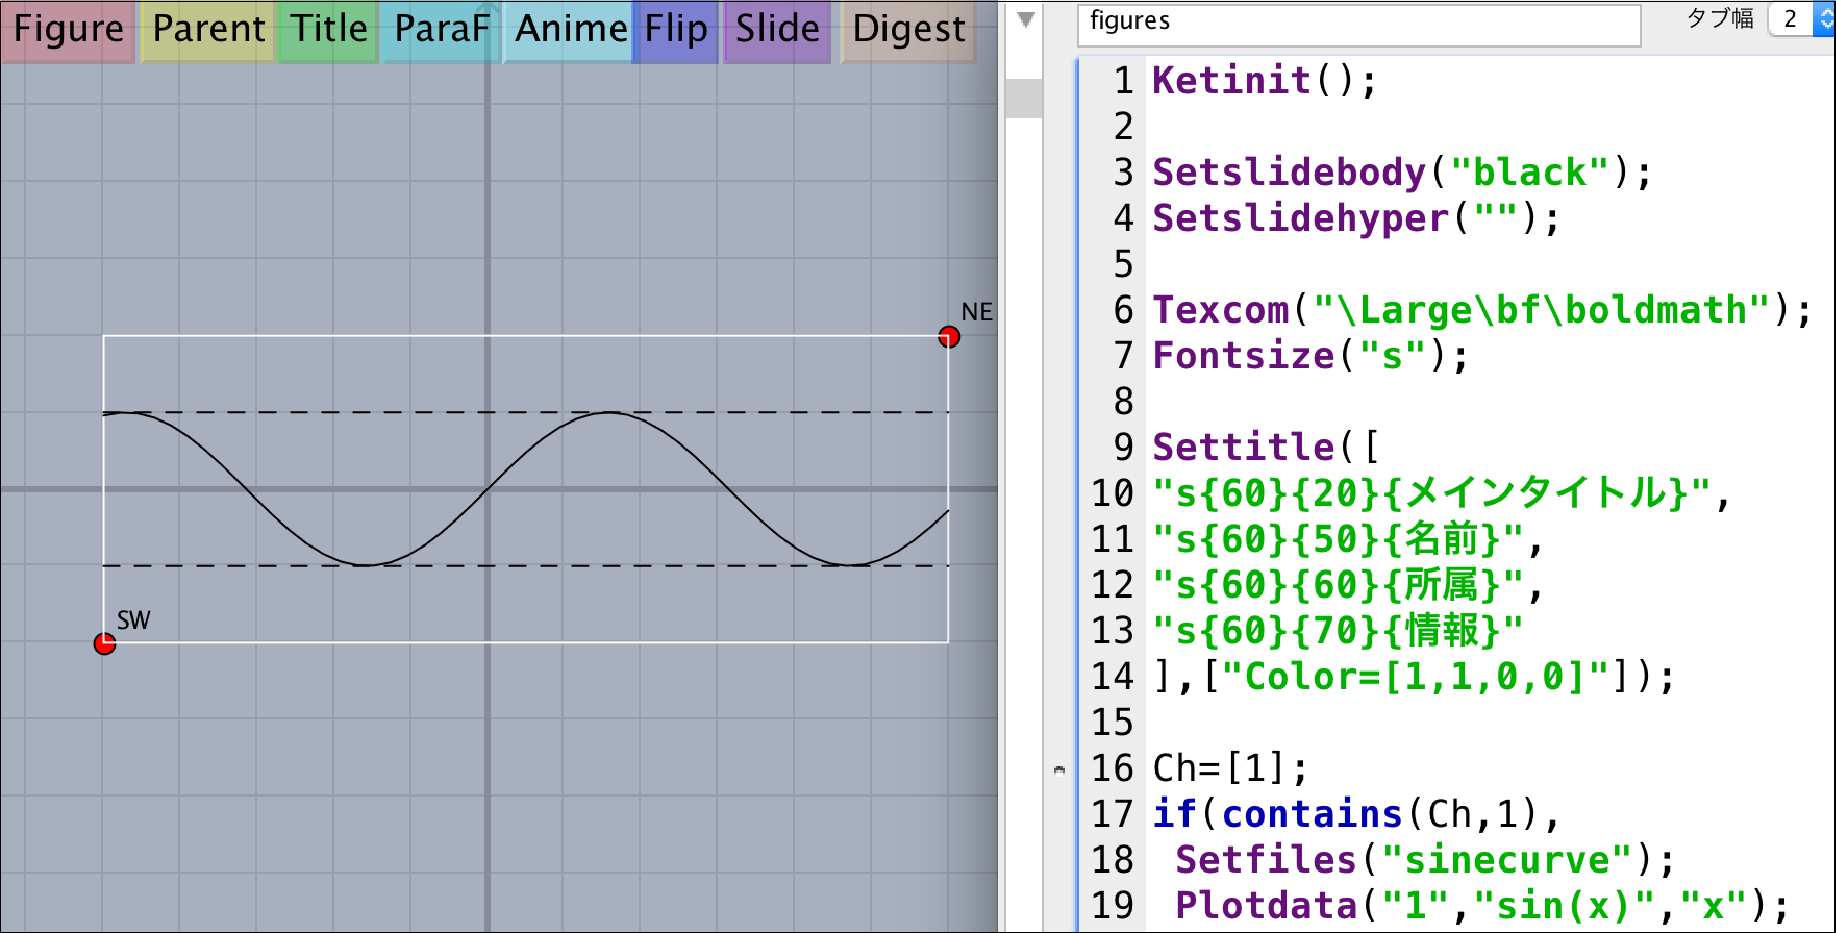
\includegraphics[bb=0.00 0.00 881.05 451.02,width=10cm]{Fig/slide01.pdf} 

\vspace{\baselineskip}
ひな形として,サンプルとして提供されている samples フォルダの中の s0701basic.cdy をコピーし,適当にリネームして使うのがよいだろう。必要なボタンと,最低限のスクリプトが記述されている。

以下では,\ketcindy のファイルを makeslide.cdy , コンテンツファイルを makeslide.txt として説明を進める。制作手順は次の通り。

(1) makeslide.cdy に \verb|Settitle| コマンドでタイトルを書き,「Titile」ボタンで書き出す。

タイトルスライドが作業フォルダに,makeslide.txt が makeslide.cdy と同じフォルダに作成される。makeslide.txt がすでにある場合には上書きはされず,タイトルスライドだけが上書きされる。

(2) makeslide.txt に,スライドの各ベージごとの内容を記述する。

(3) 必要な図やアニメーションのコードを書き,ボタンをクリックしてファイルを作る。

\hspace{10mm}Figure : 図を挿入するとき

\hspace{10mm}ParaF : アニメーションやパラパラスライドを挿入するとき

(4) Slide ボタンでスライドPDFを作成する。

PDFと,関連する中間ファイルは,作業フォルダではなく,makeslide.cdyのあるフォルダに作成される。また,スライドPDFはアニメーションと同様,Adobe Reader で開く必要がある。

\subsection{コンテンツファイル}

コンテンツファイルは次のような構成にする。

\begin{tabbing}
1234567890\=12345678912345678901234567890\=\kill
 \>title::slide0//  \> タイトルスライド。title はコマンド。\\
 \>main::三角比と三角関数//  \> セクション1のタイトル。main はコマンド。\\
 \>  直角三角形と三角比//  \> 1ページ目の表示内容。\\
 \>  ・・・・// \\
 \> new::角の概念の拡張//  \> 新しいページとタイトル。new はコマンド。\\
 \> enumerate::[(1)]// \> 2ページ目の表示内容。enumerate はコマンド。\\
 \> ・・・・//  \\
 \> new::負の角//  \> 新しいページとタイトル。\\
 \> ・・・・//  \\
 \>main::三角関数のグラフ//  \> セクション2のタイトル。\\
 \>  $f(x)=\sin x$//  \> \hspace{10mm}以下同様\\
 \> new::振幅と周期// \\
 \> ・・・・//  \\ 
\end{tabbing}
%あまりスマートな方法ではないが,枠をKeTCindyで作ってレイヤーで表示
\begin{layer}{150}{0}
\hspace{7mm}%%% /Users/Hannya/Desktop/KeTCindy/fig/boxframeslide.tex 
%%% Generator=template1basic.cdy 
{\unitlength=1cm%
\begin{picture}%
(5.89,8.46)(-0.17,-4.19)%
\special{pn 8}%
%
{%
\color[rgb]{0,0,0}%
\special{pa  2130   -24}\special{pa  2130 -1504}\special{pa  2129 -1516}\special{pa  2126 -1528}%
\special{pa  2121 -1540}\special{pa  2115 -1550}\special{pa  2107 -1560}\special{pa  2097 -1568}%
\special{pa  2087 -1574}\special{pa  2076 -1579}\special{pa  2063 -1582}\special{pa  2051 -1583}%
\special{pa  1075 -1583}\special{pa    98 -1583}\special{pa    86 -1582}\special{pa    74 -1579}%
\special{pa    63 -1574}\special{pa    52 -1568}\special{pa    43 -1560}\special{pa    35 -1550}%
\special{pa    28 -1540}\special{pa    24 -1528}\special{pa    21 -1516}\special{pa    20 -1504}%
\special{pa    20   -24}\special{pa    20  1457}\special{pa    21  1469}\special{pa    24  1481}%
\special{pa    28  1492}\special{pa    35  1503}\special{pa    43  1512}\special{pa    52  1520}%
\special{pa    63  1527}\special{pa    74  1532}\special{pa    86  1534}\special{pa    98  1535}%
\special{pa  1075  1535}\special{pa  2051  1535}\special{pa  2063  1534}\special{pa  2076  1532}%
\special{pa  2087  1527}\special{pa  2097  1520}\special{pa  2107  1512}\special{pa  2115  1503}%
\special{pa  2121  1492}\special{pa  2126  1481}\special{pa  2129  1469}\special{pa  2130  1457}%
\special{pa  2130   -24}%
\special{fp}%
}%
\end{picture}}%
\end{layer}


・すべての行の末尾には必ず // をつける。

\hspace{10mm} 注)urlの指定で // を用いるときは,$||||$ とすれば // に変換される。

・ページの内容は,コマンドでレイアウトなどを指定し,表示する文をテキストで書く。

\vspace{\baselineskip}
{\bf コマンド}

コマンドにおいて,各ブロックの引数の区切りは \verb|::| とし,各行の終わりには必ず//をつける。
 
\vspace{\baselineskip}
 {\bf 【タイトルと壁紙】}
 
 タイトルスライドをつけるときは,
 
 \hspace{10mm}\verb|title::slide0//|
 
 を1行目に置く。タイトルスライドは makeslide.cdy で作る。slide0は 初期設定のタイトルスライドのファイル名。このファイル名を変更(たとえば "start")したときは,makeslide.cdy で,Settile() のオプションに "Title=start" をつけて,ファイル名が一致するようにしておく。
 
 タイトルスライドをつけないときはスライド名をつけないでおく。
 
\hspace{10mm} \verb|title:://|

注)title コマンドは必須で,これを1行目に書かないとスライドは作成されない。

\vspace{\baselineskip}
壁紙(背景)を表示するときは,タイトルコマンドに続けて壁紙ファイル名を書く。
 
 \hspace{10mm}\verb|title::slide0::wallpaper//|
 
wallpaper は壁紙のファイル名。壁紙ファイルはTeXのファイルで,作業フォルダ(fig)に入れておく。

壁紙ファイルの一例
 
\begin{verbatim}
     {\color[cmyk]{0.6,0.2,0.8,0}\huge\rm\normalsize
    \newpage
    \begin{layer}{120}{0}
    \lineseg{0}{2}{125}{0}
    \lineseg{0}{88}{125}{0}
    \putnotese{0}{90}{\ketcindy}
    \end{layer}
    }
\end{verbatim}
 
\vspace{\baselineskip}
{\bf 【セクションタイトル】}
 
\hspace{10mm}\verb|main::セクションタイトル名//|
 
セクションを分けないときはなくてもよい。

\vspace{\baselineskip}
 {\bf 【新しいページ】}
 
\hspace{10mm}\verb|new(::行下げ)::タイトル((::位置)::読み込みファイル)//|
 
 例)\verb|new::[10]::はじめに::{50}{20}::figure//|
 
読み込みファイルの表示サイズを変更するときは
 
 \hspace{10mm}\verb|new::[10]::はじめに::{50}{20}::figure,0.8//|
 
のようにする。 

読み込みファイルがなければ,figure は省略。
 
\vspace{\baselineskip}
 {\bf 【箇条書き】}
 
番号つき箇条書きは

 \hspace{10mm}\verb|enumerate//|
 
 で,enumerate環境の始まりを示す。

番号にかっこをつけるなど,番号の形式を変えるには,

\hspace{10mm}\verb|enumerate::[(1)]|

のように,\verb|::|で区切って形式を示す。 初期設定は,かっこなしの番号。

記号つき箇条書きは

\hspace{10mm}\verb|itemize//|
 
で itemize環境の始まりを示す。記号は中黒。
  
enumerate,itemizeのいずれも

\hspace{10mm}\verb|item::文//|
 
で itemを記述する。

環境の終わりは,

\hspace{10mm}\verb|end//|

で示す。

\vspace{\baselineskip}
{\bf 【項目の順表示】}

1枚のスライド内で,項目を段階的に表示するときは,\verb|new| の次の行に

\hspace{10mm}\verb| %repeat=m(,para)//|

を書く。mは段階数で,たとえば,そのスライドの内容を3段階で表示したい場合は

\hspace{10mm}\verb| %repeat=3//|

とする。実際には3枚のスライドが作られる。

para をつけると,右下にコントローラが表示され,前後に進めやすくなる。

\hspace{10mm}\verb| %repeat=3,para//|

段階的に表示したい行の先頭に,表示する順番を,2番目以降から
\begin{verbatim}
    %[2,-]::text//
    %[3,-]::text//
\end{verbatim}

のように書く。
 
番号指定を \verb| [-, 3] | とすると,3番目まで表示する。

\verb| [1..3,5 ]| とすると,1番目から3番目までと5番目に表示する。(4番目をスキップ)

\vspace{\baselineskip}
 {\bf 【薄文字】}
 
 順表示したい項目の全体像を見せておいて,そのうちの現在までの項目を示すような場合に用いる。番号指定の前に thin をつけ,
 
 \begin{verbatim}
      %thin[2,-]::text//
      %thin[3,-]::text//
\end{verbatim}

のように書くと,現段階の項目よりあとは薄文字で表示される。
 
薄文字の濃さは,

\hspace{10mm} \verb|\setthin{alpha}//|

で指定できる。alphaは0から1までの数で, 初期設定は0.1。

\verb|\setthin{0}//| のとき,指定段階以降の項目は非表示になる。

 初期設定の薄文字の濃さは,makeslide.cdy の Setslidebodyの第3引数で設定できる。たとえば,

\hspace{10mm}\verb|Setslidebody(["","",0.2]);|

とする。

item とともに用いるときは,\verb|%thin[n,-]| を先に書く。

\vspace{\baselineskip}
【例】項目の順表示

図は,3番目のJavaまで進んだところである。右下にコントローラがある。

\begin{layer}{150}{0}
\putnotese{70}{10} {
\includegraphics[bb=0.00 0.00 777.04 516.03,width=7cm]{Fig/sliderepeat.pdf} }
\end{layer}
\begin{verbatim}
  new::プログラミング言語 //
  %repeat=6,para// 
  \slidepage// 
  itemize// 
  item::Python// 
  %thin[2,-]::item::Ruby// 
  %thin[3,-]::item::Java// 
  %thin[4,-]::item::JavaScript// 
  %thin[5,-]::item::CindyScript// 
  %thin[6,-]::item::C// 
  end// 
\end{verbatim}

\vspace{\baselineskip}
 {\bf 【図ファイルの順表示】}
 
作業フォルダ(fig)の中にあるサブフォルダ(例えばsubfig)の図ファイルすべてを順に表示する。

 パラパラ動画のときに用いる。パラパラ動画では,ParaFボタンをクリックすると,作業フォルダ(fig)の中に,動画のフレームファイルが入ったフォルダが作られる。そのフォルダのファイルをアルファベット順に表示する。もちろん,パラパラ動画以外のファイルの順表示に使ってもよい。

\verb|new| の次に
 
\hspace{10mm} \verb|%repeat=//|
 
\hspace{10mm} \verb|%para=subfig:{0}:s{60}{10}:input(:倍率)//|

を書く。TeXのソースには,
 
\hspace{10mm}\verb| layer{120}{0}, \putnotes{60}{10 初期設定put...}|

の形で書き入れられる。

また,2行に分けずに

\hspace{10mm} \verb|%repeat=,para=... |と続けて書いてもよい。
 

\vspace{\baselineskip}
{\bf 【レイヤー】}

\hspace{10mm}\verb|layer::{範囲}{0}//|

で layer環境の始まりを示す。layer環境の終わりは 

\hspace{10mm}\verb|end//|
 
 レイヤーの中に作業フォルダ(fig)にある図を表示するには
 
\hspace{10mm}\verb|putnote::方向と位置::読み込みファイル//|
 
とする。
 
 例) figure.texを(30,10)の位置の南東(原点は左上)に表示する。
 
\hspace{10mm} \verb|putonote::se{30}{10}::figure//|

 例) figの中のfigure.texを0.8倍にして表示する。
 
\hspace{10mm} \verb|putonote::se{30}{10}::figure,0.8//|
 

 例)includegraphics で figure.pdf を表示する。
 
\hspace{10mm} \verb|putonote::se{30}{10}::include[width=5cm]::figure.pdf//|
 
 
 注)\verb|KeTpicStyle.pdf|を参照。文字などは本来の書式を用いて次のように入れる。
 
\hspace{10mm} \verb|\putonotee{30}{10}{文字}//|

\vspace{\baselineskip}
{\bf 【テキストと動画】}
 
コマンド以外のテキストはそのまま \TeX\ に書き出される。行末には // をつける。
テキストを途中で改行するには,\TeX\ の 強制改行マーク \textbackslash \textbackslash をつける。

動画の場合は,動画の設定をして(アニメーションの節を参照)ファイルを作る。

パラパラ動画の場合は,ParaFボタンをクリックすると,figフォルダ内に動画のフレームファイルが入ったフォルダ(たとえば sincurve)が作られる。これを,

\hspace{10mm} \verb|%repeat=//|
 
\hspace{10mm} \verb|%para=sincurve:{0}:s{60}{10}:input(:倍率)//|

で表示する。

アニメーションの場合は,スライドのために,makeslide.cdy のスクリプトに, \verb|Addpackage(["[dvipdfmx]{animate}"]);| を追加しておく。

Animeボタンをクリックすると,パラパラアニメと同様に動画のフレームファイルが入ったフォルダが作られ,動画用の\TeX\ ファイルができる。Setpara() で設定したファイル名が "sincurve" のとき,動画用の\TeX\ ファイルは "animsincurve.tex" となるので,\verb|%repeat| ではなく \verb|\input{fig/animsincurve}//| で表示する。

 
\vspace{\baselineskip}
{\bf 【コメント行】} 

 コマンドや文をコメントアウトするときは,\verb|%%| とする。

\vspace{\baselineskip}
{\bf 【空白行】}

空白行を入れたいときは,\verb|...//| とする。

\vspace{\baselineskip}
{\bf 【タブ】}

\hspace{10mm}\verb|\Ltab{長さ}{文1}文2|

とすると,文1が行頭から,文2が長さ分の字下げをした位置から表示される。長さは 20mm のように指定。

\vspace{\baselineskip}
{\bf 【ページ番号】}

page番号を表示するときは次のようにする。
 
 mainの場合は \verb|\slidepage[m]//|
 
それ以外の場合は \verb|%repeatの後に \slidepage//|
 
 注)総ページ数を取得するため,TeXを2度コンパイルすることが必要である。そのため,Slideボタンを2度クリックすると総ページ数が表示される。

\vspace{\baselineskip}
{\bf mp3/mp4ファイルの追加}

makeslide.txtのタイトルコマンドの後に,以下を追加する。
\begin{verbatim}
  title::slide0(::wallpaper)
  ::\usepackage{ketmedia}
  ::\usepackage[dvipdfmx]{media9}//
\end{verbatim}

mp3ファイルを追加するときは,\verb|\inputsound|または\verb|\inputsoundclick|を用いる。\\
\hspace{10mm}\verb|\inputsountclik[90]{フォルダ/}{ファイル}|\\
\verb|\inputsound|は「自動再生」,\verb|\inputsoundclick|は「クリック再生」である。
最初の引数は,ボタンの水平位置(単位mm)でデフォルトは90である.またフォルダには\verb|/|をつける。\vspace{2mm}

mp4ファイルを追加するときは,\verb|\inputmovie|を用いる。\\
\hspace{10mm}\verb|\inputsountclik[90]{1}{0.4}{フォルダ/}{ファイル}|\\
2番目と3番目の引数は,幅と高さの\verb|\linewidth|からの倍率である。

\subsection{関数}
makeslide.cdy で使う,\ketcindy の関数。

\begin{description}

\hypertarget{setslidebody}{}
\item[関数]  Setslidebody(bodycolor,bodystyle,density)
\item[機能]  全体の文字スタイルと薄文字の濃さ(0-1)の設定
\item[説明]  引数の意味は次の通り。
\begin{tabbing}
1234567890123\=4567890\=\kill
bodycolor  \> 文字色 :  初期設定は "blue"\\
bodystyle  \> フォントタイプ :  初期設定は \verb|"\Large\bf\boldmath"|\\
density  \> 薄文字の濃さ :  初期設定は 0.1
\end{tabbing}

引数がない場合や( \verb|Setslidebody()|)この関数を書かない場合は初期値が使われる。

ある引数だけを指定したい場合は,それより前は空にする。

【例】\verb|Setslidebody(,"\large")|

\vspace{\baselineskip}
\hypertarget{setslidehyper}{}
\item[関数]  Setslidehyper("dvipdfmx",options)
\item[機能]  順表示でページ送りのコントローラを設定する。
\item[説明]  順表示しないときもこの関数の記述は必須と考えてよい。

パッケージ hyperref.styを読み込み,かつ,options の値を与える。

\verb|Setslidehyper();| は無効。初期設定で使う場合は \verb|Setslidehyper("");| とする。

第1引数は hyperref.sty の第1パラメータ。初期設定は "dvipdfmx"

options は ["cl=bool,lc=col,fc=col","Pos=[x,y]","Size=n"]

\begin{tabbing}
12345\=4567890\=\kill
cl \> colorlinks : リンクに色をつけるかどうか。true / false で指定。 初期設定は true\\
lc \> linkcolor : コントローラの色。色名で指定。 初期設定は blue\\
fc\> filecolor リンクの色。色名で指定。 初期設定は blue\\
以上3つは,セットで指定。一部初期値を使う場合は\verb|lc=,| のように右辺を空にする。\\
Pos \> コントローラの位置。 初期設定は [125,73] (左上が原点)\\
Size \> コントローラの大きさ。 初期設定は1
\end{tabbing}


\vspace{\baselineskip}
\hypertarget{setslidemain}{}
\item[関数]  Setslidemain([letterc,boxc,boxd,framec,xpos,size])
\item[機能]  メインスライド(セクション区切り)の設定
\item[説明]  引数の一部を 初期設定値とする場合は [,,,,3] や [,"red"] などとする。
\begin{tabbing}
1234567\=4567890\=\kill
letterc \> 文字の色。 初期設定は CMYKで [0.98,0.13,0,0.43]\\
boxc \> ボックスの色。 初期設定は [0,0.32,0.52,0] \\
frame\> フレームの色。 初期設定は [0,0.32,0.52,0]\\
xpos \> タイトルの水平位置。 初期設定は 62\\
size \> タイトルの倍率。 初期設定は 2
\end{tabbing}


\vspace{\baselineskip}
\hypertarget{setslidepage}{}
\item[関数]  Setslidepage([letterc,boxc,boxd,framec,shadowc,xpos,size])
\item[機能]  ページの設定をする。
\item[説明]  引数の一部を 初期設定値とする場合は [,,,,3] や [,"red"]などとする。

\begin{tabbing}
1234567\=4567890\=\kill
letterc \> 文字の色。 初期設定は CMYKで [0.98,0.13,0,0.43]\\
boxc \> ボックスの色。 初期設定は [0,0.32,0.52,0] \\
frame\> フレームの色。 初期設定は [0,0.32,0.52,0]\\
shadowc \> 影の色。 初期設定は [0,0,0,0.5]\\
xpos \> タイトルの水平位置。 初期設定は 6\\
size \> タイトルの倍率。 初期設定は 1.3
\end{tabbing}

\vspace{\baselineskip}
\hypertarget{setslidemargin}{}
\item[関数]  Setslidemargin([leftmarginchange,topmarginchange])
\item[機能]  スライドの左上マージンをデフォルトから変更する場合の値。
\item[説明]  Setslidemargin([+5,-10]);(横方向に$+5$mm,縦方向に$-10$mm変更)

\vspace{\baselineskip}
\hypertarget{settitle}{}
\item[関数]  Settitle(タイトルリスト,options)
\item[機能]  タイトルスライドを作る
\item[説明]  タイトルリストはコンマ区切りで位置と文を文字列で与える。例を参照。
「Title」ボタンをクリックすると,コンテンツファイルがない場合は新たに作る。すでにある場合は上書きせずタイトルスライドのみを作る。

Settitleのオプションは次をリストで与える。

\begin{tabbing}
123456789012\=4567890\=\kill
"Title=" \> タイトルスライドのファイル名。 初期設定は "slide0"。\\
"Layery=" \> タイトルの縦位置。 初期設定は0。0でないときは方眼を表示。 \\
"Color="\> 文字の色。 初期設定は blue。
\end{tabbing}

\vspace{\baselineskip}
【例】タイトルの設定

\begin{verbatim}
    Settitle([ 
      "s{60}{20}{メインタイトル}", 
      "s{60}{50}{名前}", 
      "s{60}{60}{所属}", 
      "s{60}{70}{情報}" 
    ] , 
    ["Title=SlideA","Color=[1,1,0,0]"]); 
\end{verbatim}

出力する \TeX\ ファイルに,\verb|\begin{layer}| の設定をする。 \verb|s| は,東西南北の\verb|s|  。

例のように,タイトルリストは改行すると見やすい。

\end{description}
\newpage
%================== 3D ===============
\section{\ketcindy 3D}
\subsection{概要}
\ketcindy 3Dの画面は次のように構成される。

Cinderellaの描画面に,白の矩形で囲んだ領域が2つできる。NE,SWを対角とする左側の領域を主画面,右側の領域を副画面という。

\vspace{\baselineskip}
\begin{center}
 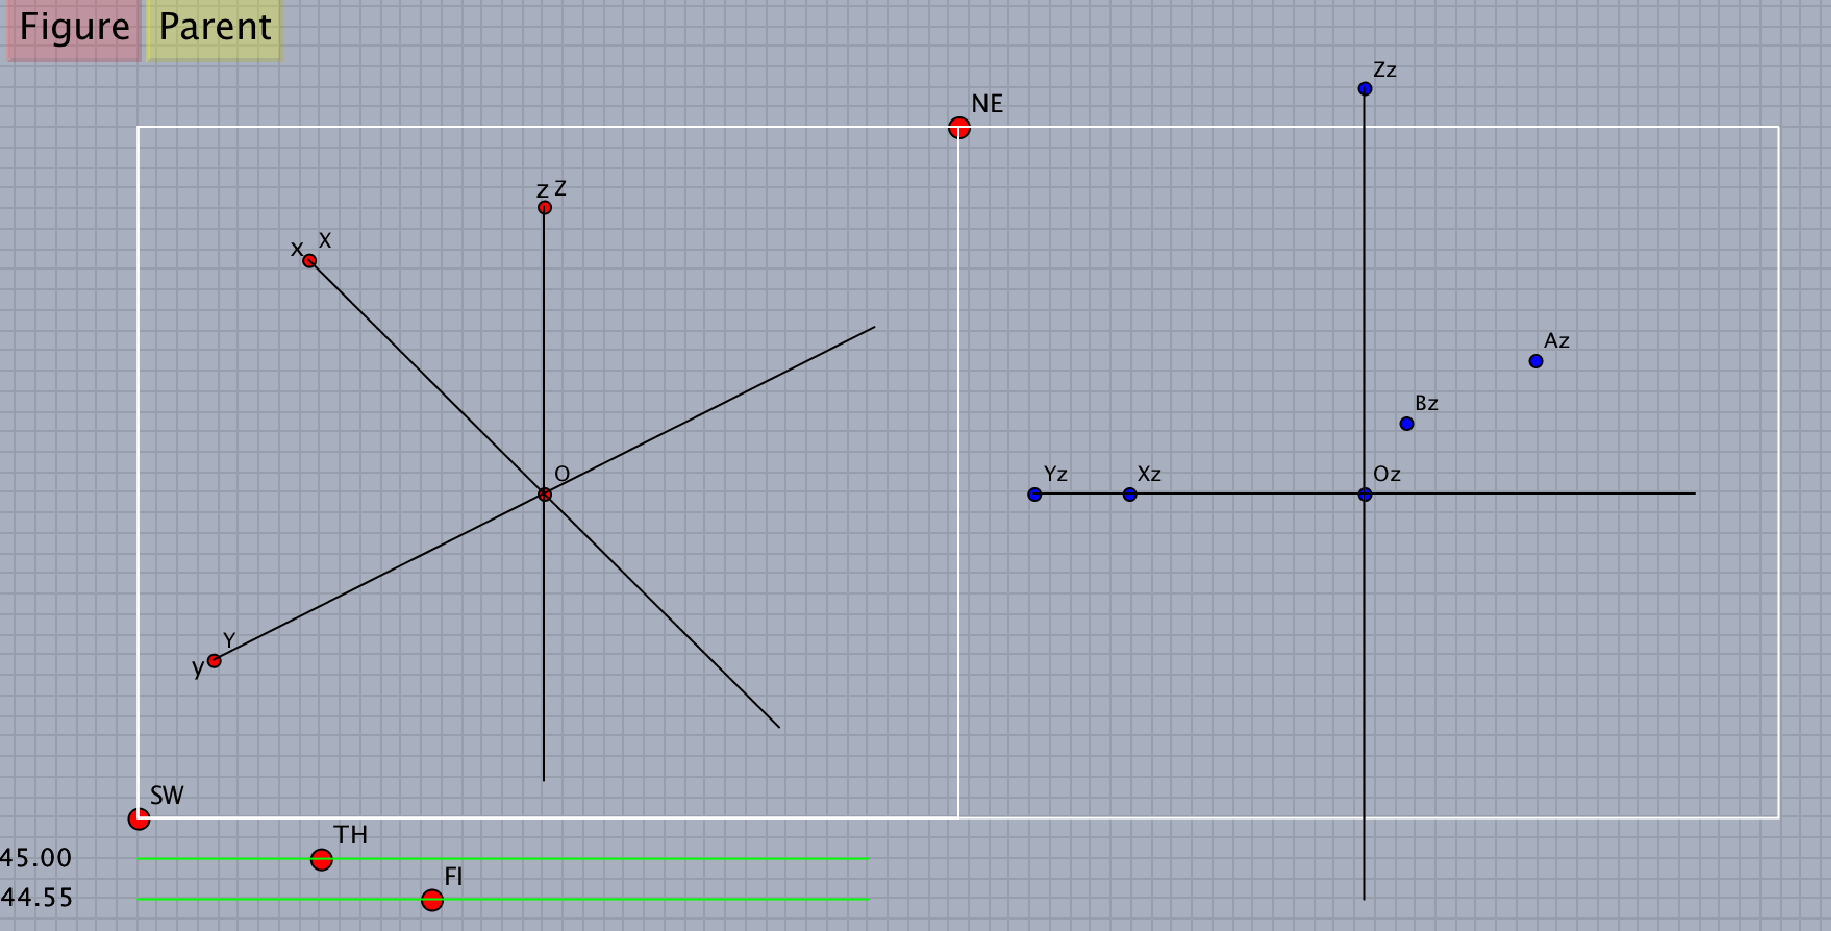
\includegraphics[bb=0 0 879.05 447.02 , width=8cm]{Fig/3dstart.pdf}
\end{center}
主画面は平面の場合と同様,TeXに出力される範囲を示し,NE,SWの2点をドラッグすることにより変更できる。主画面の下方のスライダで視点が移動でき,主画面上では軸が回転する。副画面は,xy平面上に視点を置いたものと考えればよい。

主画面上にCinderellaの作図ツールで点や線分を作図すると,副画面に対応する点が作図される。主画面上の点をドラッグするとx,y座標を変更でき,副画面上の点をドラッグするとz座標を変更できる。

\vspace{\baselineskip}
\begin{center}
 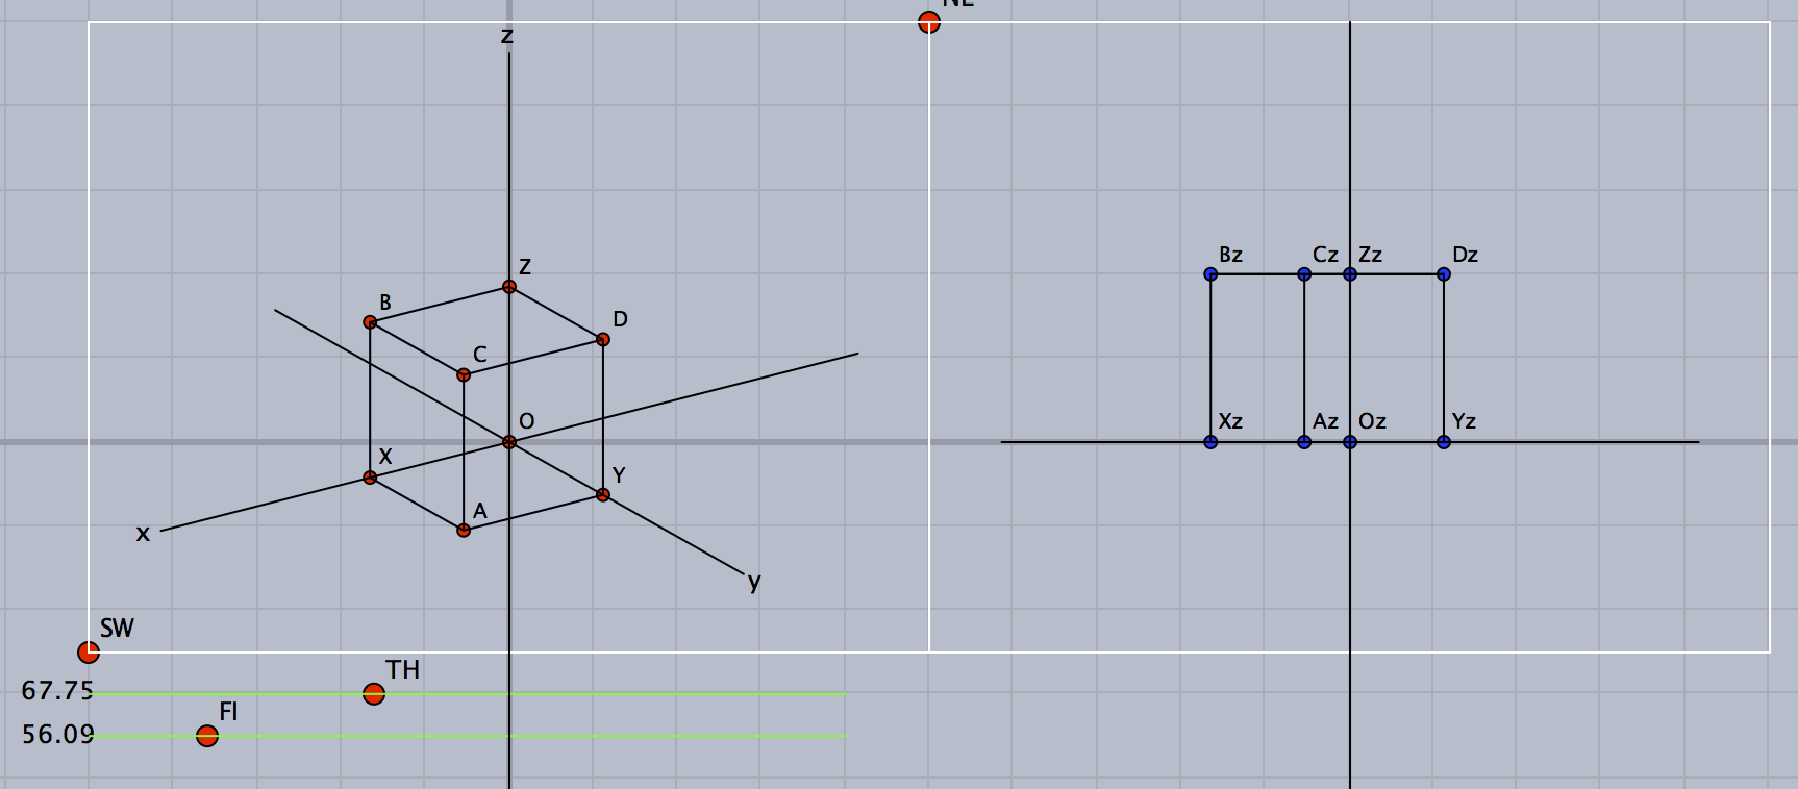
\includegraphics[bb=0.00 0.00 863.04 378.52 , width=10cm]{Fig/3dscreen.pdf}
\end{center}

KeTCindy3Dでは,線や面についての陰線処理を行う。陰線処理はC言語との連携により処理を速めている。C言語を使う環境整備が必要であるが,現在はこれを標準としている。C言語が使えない場合はRで計算する関数を用いることになるが,その場合はかなり時間がかかる。(場合にもよるが2分程度)

\newpage
\subsection{設定・定義}

\begin{description}

\hypertarget{ketinit3d}{}
\item[関数]  Ketinit3d()
\item[機能]  KeTCindy3Dの使用宣言
\item[説明]  Cinderellaの画面を3Dモードにする。

Cinderellaの描画面に,視点移動のための2つのスライダを作る。スライダは初期位置が左端になる。

\textcolor{red}{<重要>}

  この関数は Initialization スロットに置く。Ketinit() も,平面の場合と異なり Initialization スロットに置く。KeTCindy3Dにおける変数の初期化などを行う,Start3d()はDrawスロットに書く。
  
\vspace{\baselineskip}
\hypertarget{start3d}{}
\item[関数]  Start3d(option)
\item[機能]  3Dの画面設定と空間点の認識
\item[説明]  副画面を作り,幾何点を3Dの点として認識する。この関数は必須で,Drawスロットの先頭に書く。

Cinderellaの作図ツールで,点・線分を作図すると,内部関数の Ptseg3data() によってそれらを空間の点として認識し,副画面上に対応する点をとる。ただし,始めはz座標を0とする。点の名前がAであれば,副画面上の点はAzとなる。点をポイントして選択すると副画面の上に座標が表示される。

作図した点の名称をインスペクタで変更した場合,新しい名称に対応する点を副画面上に作成するが,以前の点は消えないので要注意。たとえば,点Aを作図した後,主画面上の点Aをインスペクタで点Dに変えた場合,副画面上に新たにDzができるが,以前のAzも残る。残ったAzは,選択しておいて作図ツールの消去ボタン 
\includegraphics[bb=0 0 6.48 5.04 , width=0.6cm]{Fig/delete.pdf}で消すことができる。

optionに,除外点のリストを与えると,その点は空間点としない。(始点を移動しても位置は変わらない)

\vspace{\baselineskip}
\hypertarget{startsurf}{}
\item[関数]  Startsurf(options)
\item[機能]  曲面描画の初期化と定数の設定
\item[説明]  options で定数を設定する。定数としては,分割数,Cのサイズ,誤差の限界を設定する。

optionsがないときは,以下の 初期設定を用いる。

   [50,50],[1500,500,200],[0.01,0.1]

設定後に初期値にリセットするときは,文字列 "reset" を引数に与える。

これにより,陰線処理をともなう面の描画の手順は,次のようになる。

(1)  Startsurf(); で面描画の宣言をする。

(2) 描画関数でプロットデータを作る。

(3) ExeccmdC(); で,C言語を用いてまとめて描画する。


\vspace{\baselineskip}
\hypertarget{isangle}{}
\item[関数]  Isangle()
\item[機能]  角度スライダ(視点スライダ)の選択判断
\item[説明]  角度スライダを選択しているときは true ,そうでないときは false を返す。

曲面の描画・陰線処理には時間がかかるため,角度スライダを動かすと反応が悪くなる。そこで,角度スライダを選択しているときは曲面の描画をしないようにすることで反応がよくなる。

\vspace{\baselineskip}
【例】放物面の描画

次のようにすると,スライダの点を選んでいる間はワイヤフレームモデルが描かれ,画面上の他の部分をクリックして選択状態が解除されると陰線処理された放物面が描かれる。
\begin{verbatim}
    fd=[
     "z=4-(x^2+y^2)",
     "x=R*cos(T)","y=R*sin(T)",
     "R=[0,2]","T=[0,2*pi]","e"
    ];
    if(Isangle(),
     Sf3data("1",fd);
     ,
     Startsurf();
     Sfbdparadata("1",fd);
     Crvsfparadata("1","ax3d","sfbd3d1",fd);
     ExeccmdC("1");
   );
\end{verbatim}

\end{description}

\begin{flushright} \hyperlink{functionlist}{$\Rightarrow$関数一覧}\end{flushright}

\newpage
\subsection{描画}
\begin{description}

\hypertarget{bezier3d}{}
\item[関数]  Bezier3d(name,リスト1,リスト2)
\item[機能]  空間ベジェ曲線を描く
\item[説明]  引数はリスト1が端点リスト,リスト2が制御点リスト

1組の端点につき,2つの制御点を使う。

\vspace{\baselineskip}
【例】いくつかの点をベジェ曲線で結ぶ

  端点A,Bに対し,制御点をD,Eとする。
  
    \verb|Bezier3d("1",["A","B"],["D","E"]);| \vspace{\baselineskip}

  端点A,Bに対し,制御点をD,Eとし,端点BCに対し制御点をE,Fとする。
  
    \verb|Bezier3d("1",["A","B","C"],["D","E","E","F"]);|
    
 端点A,Bに対し,制御点をD,Eとし,端点BCに対し制御点をF,Gとする。(図)
 
    \verb|Bezier3d("1",["A","B","C"],["D","E","F","G"]);|
    
    \begin{center} %%% /Users/Hannya/ketcindy/ketwork/template.tex 2016-8-14 11:12
%%% template.sce 2016-8-14 11:12
{\unitlength=8mm%
\begin{picture}%
(   9.74000,   5.94000)(  -4.74000,  -1.94000)%
\special{pn 8}%
%
\settowidth{\Width}{$x$}\setlength{\Width}{-0.5\Width}%
\settoheight{\Height}{$x$}\settodepth{\Depth}{$x$}\setlength{\Height}{-0.5\Height}\setlength{\Depth}{0.5\Depth}\addtolength{\Height}{\Depth}%
\put(-3.2520,-1.0065){\hspace*{\Width}\raisebox{\Height}{$x$}}%
%
%
\settowidth{\Width}{$y$}\setlength{\Width}{-0.5\Width}%
\settoheight{\Height}{$y$}\settodepth{\Depth}{$y$}\setlength{\Height}{-0.5\Height}\setlength{\Depth}{0.5\Depth}\addtolength{\Height}{\Depth}%
\put(3.3782,-1.4998){\hspace*{\Width}\raisebox{\Height}{$y$}}%
%
%
\settowidth{\Width}{$z$}\setlength{\Width}{-0.5\Width}%
\settoheight{\Height}{$z$}\settodepth{\Depth}{$z$}\setlength{\Height}{-0.5\Height}\setlength{\Depth}{0.5\Depth}\addtolength{\Height}{\Depth}%
\put(0.0000,3.9050){\hspace*{\Width}\raisebox{\Height}{$z$}}%
%
%
\special{pa 1209 -374}\special{pa -967 299}%
\special{fp}%
\special{pa -1009 -448}\special{pa 1009 448}%
\special{fp}%
\special{pa 0 611}\special{pa 0 -1170}%
\special{fp}%
\special{pa -903 254}\special{pa -967 299}\special{pa -888 300}\special{pa -896 277}%
\special{pa -903 254}\special{sh 1}\special{ip}%
\special{pn 1}%
\special{pa -903 254}\special{pa -967 299}\special{pa -888 300}\special{pa -896 277}%
\special{pa -903 254}\special{pa -967 299}%
\special{fp}%
\special{pn 8}%
\special{pa 931 440}\special{pa 1009 448}\special{pa 951 395}\special{pa 941 418}%
\special{pa 931 440}\special{sh 1}\special{ip}%
\special{pn 1}%
\special{pa 931 440}\special{pa 1009 448}\special{pa 951 395}\special{pa 941 418}%
\special{pa 931 440}\special{pa 1009 448}%
\special{fp}%
\special{pn 8}%
\special{pa 24 -1095}\special{pa 0 -1170}\special{pa -24 -1095}\special{pa 0 -1095}%
\special{pa 24 -1095}\special{sh 1}\special{ip}%
\special{pn 1}%
\special{pa 24 -1095}\special{pa 0 -1170}\special{pa -24 -1095}\special{pa 0 -1095}%
\special{pa 24 -1095}\special{pa 0 -1170}%
\special{fp}%
\special{pn 8}%
\settowidth{\Width}{O}\setlength{\Width}{0\Width}%
\settoheight{\Height}{O}\settodepth{\Depth}{O}\setlength{\Height}{\Depth}%
\put(0.1500,0.1500){\hspace*{\Width}\raisebox{\Height}{O}}%
%
%
\special{pa -484 150}\special{pa -437 81}\special{pa -387 31}\special{pa -335 -1}%
\special{pa -282 -19}\special{pa -227 -23}\special{pa -171 -16}\special{pa -115 0}%
\special{pa -60 23}\special{pa -5 52}\special{pa 49 84}\special{pa 101 116}\special{pa 151 148}%
\special{pa 199 177}\special{pa 243 201}\special{pa 284 219}\special{pa 321 227}\special{pa 354 225}%
\special{pa 382 209}\special{pa 404 179}\special{pa 423 90}\special{pa 433 13}\special{pa 435 -52}%
\special{pa 429 -108}\special{pa 417 -154}\special{pa 399 -193}\special{pa 376 -226}%
\special{pa 349 -253}\special{pa 319 -277}\special{pa 286 -298}\special{pa 251 -319}%
\special{pa 215 -339}\special{pa 178 -360}\special{pa 143 -384}\special{pa 108 -411}%
\special{pa 76 -444}\special{pa 47 -483}\special{pa 21 -530}\special{pa 0 -585}%
\special{fp}%
\special{pn 1}%
\special{pa -475 141}\special{pa -482 138}\special{pa -489 139}\special{pa -494 144}%
\special{pa -495 152}\special{pa -492 158}\special{pa -485 161}\special{pa -478 160}%
\special{pa -473 155}\special{pa -472 148}\special{pa -475 141}\special{sh 1}\special{fp}%
\special{pa 412 171}\special{pa 406 168}\special{pa 398 169}\special{pa 393 174}\special{pa 392 181}%
\special{pa 395 188}\special{pa 402 191}\special{pa 409 190}\special{pa 414 185}\special{pa 415 177}%
\special{pa 412 171}\special{sh 1}\special{fp}%
\special{pa 8 -593}\special{pa 2 -597}\special{pa -5 -596}\special{pa -11 -590}\special{pa -12 -583}%
\special{pa -8 -577}\special{pa -2 -573}\special{pa 5 -575}\special{pa 11 -580}\special{pa 12 -587}%
\special{pa 8 -593}\special{sh 1}\special{fp}%
\special{pa -187 -360}\special{pa -194 -363}\special{pa -201 -362}\special{pa -206 -357}%
\special{pa -207 -350}\special{pa -204 -343}\special{pa -197 -340}\special{pa -190 -341}%
\special{pa -185 -346}\special{pa -184 -354}\special{pa -187 -360}\special{sh 1}\special{fp}%
\special{pa 290 414}\special{pa 283 410}\special{pa 276 411}\special{pa 271 417}\special{pa 270 424}%
\special{pa 273 430}\special{pa 279 434}\special{pa 287 433}\special{pa 292 427}\special{pa 293 420}%
\special{pa 290 414}\special{sh 1}\special{fp}%
\special{pa 563 -438}\special{pa 557 -441}\special{pa 549 -440}\special{pa 544 -435}%
\special{pa 543 -428}\special{pa 546 -421}\special{pa 553 -418}\special{pa 560 -419}%
\special{pa 565 -424}\special{pa 567 -432}\special{pa 563 -438}\special{sh 1}\special{fp}%
\special{pa 126 -212}\special{pa 119 -215}\special{pa 112 -214}\special{pa 107 -209}%
\special{pa 106 -201}\special{pa 109 -195}\special{pa 115 -192}\special{pa 123 -193}%
\special{pa 128 -198}\special{pa 129 -205}\special{pa 126 -212}\special{sh 1}\special{fp}%
\special{pn 8}%
\settowidth{\Width}{A}\setlength{\Width}{-0.5\Width}%
\settoheight{\Height}{A}\settodepth{\Depth}{A}\setlength{\Height}{-\Height}%
\put(-1.5352,-0.5252){\hspace*{\Width}\raisebox{\Height}{A}}%
%
%
\settowidth{\Width}{B}\setlength{\Width}{0\Width}%
\settoheight{\Height}{B}\settodepth{\Depth}{B}\setlength{\Height}{\Depth}%
\put(1.3318,-0.5191){\hspace*{\Width}\raisebox{\Height}{B}}%
%
%
\settowidth{\Width}{C}\setlength{\Width}{0\Width}%
\settoheight{\Height}{C}\settodepth{\Depth}{C}\setlength{\Height}{\Depth}%
\put(0.0500,1.9075){\hspace*{\Width}\raisebox{\Height}{C}}%
%
%
\settowidth{\Width}{D}\setlength{\Width}{0\Width}%
\settoheight{\Height}{D}\settodepth{\Depth}{D}\setlength{\Height}{\Depth}%
\put(-0.5703,1.1665){\hspace*{\Width}\raisebox{\Height}{D}}%
%
%
\settowidth{\Width}{E}\setlength{\Width}{0\Width}%
\settoheight{\Height}{E}\settodepth{\Depth}{E}\setlength{\Height}{-\Height}%
\put(0.9432,-1.3898){\hspace*{\Width}\raisebox{\Height}{E}}%
%
%
\settowidth{\Width}{F}\setlength{\Width}{0\Width}%
\settoheight{\Height}{F}\settodepth{\Depth}{F}\setlength{\Height}{\Depth}%
\put(1.8116,1.4146){\hspace*{\Width}\raisebox{\Height}{F}}%
%
%
\settowidth{\Width}{G}\setlength{\Width}{0\Width}%
\settoheight{\Height}{G}\settodepth{\Depth}{G}\setlength{\Height}{\Depth}%
\put(0.4222,0.6951){\hspace*{\Width}\raisebox{\Height}{G}}%
%
%
\end{picture}}% \end{center}

\begin{flushright} \hyperlink{functionlist}{$\Rightarrow$関数一覧}\end{flushright}

\hypertarget{changestyle3d}{}
\item[関数]  Changestyle3d(リスト,リスト)
\item[機能]  3Dプロットデータの属性を変更
\item[説明]  第1引数のプロットデータの属性を,第2引数に変更する。

たとえば,補助線など,画面には描いてもTeXに書き出さない線を描画するときは,optionに["notex"] をつけるが,これをあとから付加したい場合に利用する。プロットデータはリストにできるので,複数のプロットデータの属性をまとめて変更することができて便利である。

\vspace{\baselineskip}
【例】4つの点で四面体の辺を描き,まとめて notex にする。点A,B,C,Dはとってあるものとする。
\begin{verbatim}
  Spaceline("1",[A,B]);
  Spaceline("2",[A,C]);
  Spaceline("3",[B,C]);
  Spaceline("4",[A,D]);
  Spaceline("5",[B,D]);
  Spaceline("6",[C,D]);
  edges=apply(1..6,"sl3d"+text(#));
  Changestyle3d(edges,["notex"]);
\end{verbatim}

\hypertarget{concatobj}{}    
\item[関数]  Concatobj(リスト,option)
\item[機能]  いくつかのobjデータを結合する
\item[説明]  多面体の各面の頂点リストから面データ(頂点リストと面リスト)を作る。

\vspace{\baselineskip}
【例】4点A,B,C,Dを頂点とする四面体を描く。

四面体は4つの面からなっている。頂点をA,B,C,Dとすると,4つの面は
  
              △ABC,△ABD,△ACD,△BCD\\
である。
  
        \begin{center} %%% /Users/Hannya/ketcindy/ketwork/template.tex 2016-8-24 20:24
%%% template.sce 2016-8-24 20:24
{\unitlength=8mm%
\begin{picture}%
(   5.00000,   5.00000)(  -3.00000,  -1.00000)%
\special{pn 8}%
%
\special{pa 483 -179}\special{pa 185 -147}%
\special{fp}%
\special{pa 137 -141}\special{pa -712 -48}%
\special{fp}%
\special{pa -712 -48}\special{pa 229 228}%
\special{fp}%
\special{pa 483 -179}\special{pa 229 228}%
\special{fp}%
\special{pa -712 -48}\special{pa 0 -1030}%
\special{fp}%
\special{pa 483 -179}\special{pa 0 -1030}%
\special{fp}%
\special{pa 229 228}\special{pa 0 -1030}%
\special{fp}%
\settowidth{\Width}{A}\setlength{\Width}{-1\Width}%
\settoheight{\Height}{A}\settodepth{\Depth}{A}\setlength{\Height}{\Depth}%
\put(-0.0500,3.3201){\hspace*{\Width}\raisebox{\Height}{A}}%
%
%
\settowidth{\Width}{B}\setlength{\Width}{-1\Width}%
\settoheight{\Height}{B}\settodepth{\Depth}{B}\setlength{\Height}{-0.5\Height}\setlength{\Depth}{0.5\Depth}\addtolength{\Height}{\Depth}%
\put(-2.4118,0.1538){\hspace*{\Width}\raisebox{\Height}{B}}%
%
%
\settowidth{\Width}{C}\setlength{\Width}{0\Width}%
\settoheight{\Height}{C}\settodepth{\Depth}{C}\setlength{\Height}{-\Height}%
\put(0.7771,-0.7732){\hspace*{\Width}\raisebox{\Height}{C}}%
%
%
\settowidth{\Width}{D}\setlength{\Width}{0\Width}%
\settoheight{\Height}{D}\settodepth{\Depth}{D}\setlength{\Height}{\Depth}%
\put(1.5848,0.6193){\hspace*{\Width}\raisebox{\Height}{D}}%
%
%
\end{picture}}% \end{center}
  
そこで
  
    \verb|Concatobj([[A,B,C],[A,B,D],[A,C,D],[B,C,D]]);|
    
とすると,面データ  [[A,B,C,D],[[1,2,3],[1,2,4],[1,3,4],[2,3,4]]]   が返される。
  
この面データを使って四面体を描くことができる。コード例は,\hyperlink{vertexedgeface}{VertexEdgeFace()} を参照のこと。

\begin{flushright} \hyperlink{functionlist}{$\Rightarrow$関数一覧}\end{flushright}

\hypertarget{crvsfparadata}{}
\item[関数]  Crvsfparadata(name,PD1,PD2,式)
\item[機能]  曲面による曲線の陰線処理を行う。
\item[説明]  曲線PD1を表示するにあたり,曲面PD2によって隠れる部分処理を行う。

曲面PD2のプロットデータを作るため,Sfbdparadata() も同時に用いることになる。nameは,Sfbdparadata() と同じものにする。

作図例は,\hyperlink{execcmdc}{ExeccmdC()} を参照のこと。

C言語が使えない場合は,CrvsfparadataR(name,PD1,PD2,式,options1,options2) を使う。
options1 は分割数と誤差限界, options2 は陰線の線種。

\vspace{\baselineskip}
\hypertarget{datalist}{}    
\item[関数]  Datalist2d()
\item[機能]  画面上のプロットデータのリストを取得する
\item[説明]  画面に描かれているすべてのプロットデータのリストを返す。

空間図形は,Cinderellaの画面上に射影し表示する。そのため,KeTCindy3Dは,空間におけるプロットデータと,画面上に表示するプロットデータの2つを作っている。Datalist2d()では,画面上に表示するプロットデータのリストを返す。

\vspace{\baselineskip}
【例】
\begin{verbatim}
  Xyzax3data("","x=[-5,5]","y=[-5,5]","z=[-5,5]");
  Putpoint3d(["A",[0,-3,0],"B",[0,3,3]],"fix");
  Spaceline("1",[A,B]);
  println("PD="+Datalist2d());
\end{verbatim}
とすると,コンソールに  PD=[ax2d,AB2d]   と表示される。ax2dは座標軸のプロットデータ ax3d に,AB2d は線分ABのプロットデータ AB3d に対応している。

\vspace{\baselineskip}
\hypertarget{datalist}{}
\item[関数]  Datalist3d()
\item[機能]  空間のプロットデータのリストを取得する
\item[説明]  空間に描かれているすべてのプロットデータのリストを返す

\vspace{\baselineskip}
【例】
\begin{verbatim}
  Xyzax3data("","x=[-5,5]","y=[-5,5]","z=[-5,5]");
  Putpoint3d(["A",[0,-3,0],"B",[0,3,3]],"fix");
  Spaceline("1",[A,B]);
  println("PD="+Datalist3d());
\end{verbatim}
とすると,コンソールに  PD=[ax3d,AB3d]   と表示される。


\begin{flushright} \hyperlink{functionlist}{$\Rightarrow$関数一覧}\end{flushright}

\hypertarget{dist3d}{}
\item[関数]  Dist3d(a1,a2)
\item[機能]  空間の2点間の距離を返す
\item[説明]  引数a1,a2 は作図点の名称,空間点の名称のいずれでもよい。

次の3通りの記法は同じ結果を返す。混在も可
\begin{verbatim}
  Dist3d("A","B");
  Dist3d(A,B);
  Dist3d(A3d,B3d);
\end{verbatim}
\vspace{\baselineskip}

\hypertarget{drawpoint3d}{}
\item[関数]  Drawpoint3d(座標)
\item[機能]  空間点を描く
\item[説明]  引数で与えた空間座標の点を描く。この点は幾何点ではない。また,TeX にも出力されない。幾何点にするには \hyperlink{putpoint3d}{Putpoint3d()} を用いる。TeXに点を出力するには,\hyperlink{pointdata3d}{Pointdata3d()} を用いる。

引数は,座標のリストにすることもできる。\\
\vspace{\baselineskip}
【例】
\begin{verbatim}
  Drawpoint3d([1,1,1]);
  Drawpoint3d([[1,1,1],[0,1,0]]);
\end{verbatim}
\vspace{\baselineskip}

\hypertarget{execcmdc}{}
\item[関数]  ExeccmdC(name,options1,options2)
\item[機能]  曲面を表示する。戻り値は,対象にしたプロットデータのリスト。
\item[説明]  データが作成された曲面を表示する。

options1 には"r","m", "Wait=n" と輪郭線の線種が指定できる。Wait の初期値は20

  "r","m"に関しては,オプションなしまたは,”” のとき
  
    i) データファイルがなければ,新しく作る
    
    ii) データファイルが既にあればそれを読み込む
    
  "m"  のとき,強制的にデータファイルを作り直す。
  
  "r" のとき,すでにあるデータファイルを読み込む。
  
options2 には 軸の陰線について "nodisp" または線種が指定できる。 初期設定は "do"。

options2だけを指定したい場合は,options1 を空リスト [ ] にする。


\vspace{\baselineskip}
【例】回転放物面と座標軸,線分を陰線処理したデータを作って表示する。線分の端点A,Bはあらかじめ作図しておく。

 初期設定では陰線は点線で表示される。(下図左)
\begin{verbatim}
    Xyzax3data("","x=[-5,5]","y=[-5,5]","z=[-5,5]");
    Putpoint3d(["A",[0,-3,0],"B",[0,3,3]],"fix");
    Spaceline([A,B]);
    fd=["z=4-(x^2+y^2)","x=R*cos(T)","y=R*sin(T)","R=[0,2]","T=[0,2*pi]","e"];
    Startsurf();
    Sfbdparadata("1",fd);
    Crvsfparadata("1","AB3d","sfbd3d1",fd);
    Crvsfparadata("2","ax3d","sfbd3d1",fd);
    ExeccmdC("1");
\end{verbatim}
options2を ["nodisp"] にすると,陰線は非表示になる。(下図右)
\begin{verbatim}
    ExeccmdC("1",[],["nodisp"]);
\end{verbatim}

        \begin{center} %%% /Users/Hannya/ketcindy/ketwork/template.tex 2016-8-24 21:3
%%% template.sce 2016-8-24 21:3
{\unitlength=6mm%
\begin{picture}%
(   6.81000,   6.95000)(  -3.50000,  -2.00000)%
\special{pn 8}%
%
\settowidth{\Width}{$x$}\setlength{\Width}{-0.5\Width}%
\settoheight{\Height}{$x$}\settodepth{\Depth}{$x$}\setlength{\Height}{-0.5\Height}\setlength{\Depth}{0.5\Depth}\addtolength{\Height}{\Depth}%
\put(-2.7936,-1.0660){\hspace*{\Width}\raisebox{\Height}{$x$}}%
%
%
\settowidth{\Width}{$y$}\setlength{\Width}{-0.5\Width}%
\settoheight{\Height}{$y$}\settodepth{\Depth}{$y$}\setlength{\Height}{-0.5\Height}\setlength{\Depth}{0.5\Depth}\addtolength{\Height}{\Depth}%
\put(3.9651,-1.1310){\hspace*{\Width}\raisebox{\Height}{$y$}}%
%
%
\settowidth{\Width}{$z$}\setlength{\Width}{-0.5\Width}%
\settoheight{\Height}{$z$}\settodepth{\Depth}{$z$}\setlength{\Height}{-0.5\Height}\setlength{\Depth}{0.5\Depth}\addtolength{\Height}{\Depth}%
\put(0.0000,4.4380){\hspace*{\Width}\raisebox{\Height}{$z$}}%
%
%
\special{pa 471 -14}\special{pa 461 -50}\special{pa 451 -85}\special{pa 442 -120}%
\special{pa 432 -153}\special{pa 422 -186}\special{pa 413 -219}\special{pa 403 -250}%
\special{pa 393 -281}\special{pa 383 -311}\special{pa 374 -341}\special{pa 364 -369}%
\special{pa 354 -397}\special{pa 345 -424}\special{pa 335 -451}\special{pa 325 -476}%
\special{pa 315 -501}\special{pa 306 -525}\special{pa 296 -549}\special{pa 286 -571}%
\special{pa 277 -593}\special{pa 268 -611}\special{pa 257 -635}\special{pa 247 -654}%
\special{pa 237 -673}\special{pa 228 -692}\special{pa 218 -709}\special{pa 208 -726}%
\special{pa 198 -742}\special{pa 188 -757}\special{pa 178 -772}\special{pa 169 -785}%
\special{pa 159 -798}\special{pa 149 -810}\special{pa 143 -817}\special{pa 139 -822}%
\special{pa 129 -833}\special{pa 118 -843}\special{pa 108 -852}\special{pa 98 -861}%
\special{pa 87 -868}\special{pa 76 -876}\special{pa 69 -880}\special{pa 53 -887}\special{pa 41 -892}%
\special{pa 31 -895}\special{pa 25 -896}\special{pa 17 -898}\special{pa 6 -899}\special{pa -5 -899}%
\special{pa -16 -898}\special{pa -23 -897}\special{pa -30 -895}\special{pa -39 -893}%
\special{pa -51 -888}\special{pa -65 -882}\special{pa -76 -876}\special{pa -87 -868}%
\special{pa -98 -861}\special{pa -108 -852}\special{pa -118 -843}\special{pa -129 -833}%
\special{pa -135 -826}\special{pa -149 -810}\special{pa -159 -798}\special{pa -169 -785}%
\special{pa -178 -772}\special{pa -188 -757}\special{pa -198 -742}\special{pa -208 -726}%
\special{pa -218 -709}\special{pa -228 -692}\special{pa -237 -673}\special{pa -243 -662}%
\special{pa -247 -654}\special{pa -257 -635}\special{pa -267 -614}\special{pa -277 -593}%
\special{pa -286 -571}\special{pa -296 -549}\special{pa -306 -525}\special{pa -315 -501}%
\special{pa -325 -476}\special{pa -335 -451}\special{pa -345 -424}\special{pa -354 -397}%
\special{pa -364 -369}\special{pa -374 -341}\special{pa -383 -311}\special{pa -393 -281}%
\special{pa -403 -250}\special{pa -413 -219}\special{pa -422 -186}\special{pa -432 -153}%
\special{pa -442 -120}\special{pa -451 -85}\special{pa -461 -50}\special{pa -471 -14}%
\special{fp}%
\special{pa -309 118}\special{pa -262 130}\special{pa -210 140}\special{pa -156 147}%
\special{pa -99 152}\special{pa -40 155}\special{pa 19 156}\special{pa 78 154}\special{pa 136 149}%
\special{pa 192 142}\special{pa 244 133}\special{pa 293 122}\special{pa 337 109}\special{pa 376 94}%
\special{pa 409 78}\special{pa 435 61}\special{pa 455 42}\special{pa 467 23}\special{pa 472 3}%
\special{pa 470 -16}\special{pa 460 -35}%
\special{fp}%
\special{pa -467 -23}\special{pa -472 -3}\special{pa -470 16}\special{pa -460 35}%
\special{pa -443 54}\special{pa -419 72}\special{pa -388 89}\special{pa -351 104}%
\special{pa -309 118}%
\special{fp}%
\special{pn 8}%
\special{pa 463 -33}\special{pa 457 -38}\special{fp}\special{pa 435 -60}\special{pa 428 -65}\special{fp}%
\special{pa 402 -82}\special{pa 395 -85}\special{fp}\special{pa 366 -98}\special{pa 358 -101}\special{fp}%
\special{pa 329 -112}\special{pa 321 -114}\special{fp}\special{pa 291 -122}\special{pa 283 -124}\special{fp}%
\special{pa 252 -132}\special{pa 244 -133}\special{fp}\special{pa 213 -139}\special{pa 205 -140}\special{fp}%
\special{pa 174 -145}\special{pa 166 -146}\special{fp}\special{pa 135 -149}\special{pa 127 -150}\special{fp}%
\special{pa 96 -153}\special{pa 88 -153}\special{fp}\special{pa 56 -155}\special{pa 48 -155}\special{fp}%
\special{pa 17 -155}\special{pa 9 -156}\special{fp}\special{pa -23 -156}\special{pa -31 -155}\special{fp}%
\special{pa -63 -154}\special{pa -71 -154}\special{fp}\special{pa -102 -152}\special{pa -110 -151}\special{fp}%
\special{pa -141 -149}\special{pa -149 -148}\special{fp}\special{pa -181 -144}\special{pa -189 -143}\special{fp}%
\special{pa -220 -138}\special{pa -228 -136}\special{fp}\special{pa -258 -130}\special{pa -266 -128}\special{fp}%
\special{pa -297 -121}\special{pa -305 -119}\special{fp}\special{pa -335 -110}\special{pa -342 -107}\special{fp}%
\special{pa -372 -96}\special{pa -379 -93}\special{fp}\special{pa -407 -79}\special{pa -414 -75}\special{fp}%
\special{pa -440 -56}\special{pa -446 -51}\special{fp}\special{pa -465 -26}\special{pa -470 -20}\special{fp}%
\special{pn 8}%
\special{pa -536 -153}\special{pa -424 -191}%
\special{fp}%
\special{pa 241 -416}\special{pa 536 -516}%
\special{fp}%
\special{pn 8}%
\special{pa -428 -190}\special{pa -420 -192}\special{fp}\special{pa -391 -202}\special{pa -383 -205}\special{fp}%
\special{pa -354 -215}\special{pa -346 -217}\special{fp}\special{pa -317 -227}\special{pa -309 -230}\special{fp}%
\special{pa -280 -240}\special{pa -272 -242}\special{fp}\special{pa -243 -252}\special{pa -235 -255}\special{fp}%
\special{pa -206 -265}\special{pa -198 -267}\special{fp}\special{pa -169 -277}\special{pa -161 -280}\special{fp}%
\special{pa -132 -290}\special{pa -124 -292}\special{fp}\special{pa -95 -302}\special{pa -87 -305}\special{fp}%
\special{pa -58 -315}\special{pa -50 -317}\special{fp}\special{pa -21 -327}\special{pa -14 -330}\special{fp}%
\special{pa 16 -340}\special{pa 23 -342}\special{fp}\special{pa 53 -352}\special{pa 60 -355}\special{fp}%
\special{pa 90 -365}\special{pa 97 -367}\special{fp}\special{pa 127 -377}\special{pa 134 -380}\special{fp}%
\special{pa 164 -390}\special{pa 171 -392}\special{fp}\special{pa 201 -402}\special{pa 208 -405}\special{fp}%
\special{pa 238 -415}\special{pa 245 -418}\special{fp}\special{pn 8}%
\special{pa 772 -295}\special{pa 429 -164}%
\special{fp}%
\special{pa -309 118}\special{pa -618 236}%
\special{fp}%
\special{pa -827 -236}\special{pa -440 -125}%
\special{fp}%
\special{pa 357 102}\special{pa 782 223}%
\special{fp}%
\special{pa 0 472}\special{pa 0 156}%
\special{fp}%
\special{pa 0 -899}\special{pa 0 -1003}%
\special{fp}%
\special{pn 8}%
\special{pa 433 -165}\special{pa 425 -162}\special{fp}\special{pa 396 -151}\special{pa 388 -148}\special{fp}%
\special{pa 359 -137}\special{pa 351 -134}\special{fp}\special{pa 322 -123}\special{pa 314 -120}\special{fp}%
\special{pa 285 -109}\special{pa 278 -106}\special{fp}\special{pa 248 -95}\special{pa 241 -92}\special{fp}%
\special{pa 211 -81}\special{pa 204 -78}\special{fp}\special{pa 174 -67}\special{pa 167 -64}\special{fp}%
\special{pa 137 -52}\special{pa 130 -50}\special{fp}\special{pa 101 -38}\special{pa 93 -36}\special{fp}%
\special{pa 64 -24}\special{pa 56 -21}\special{fp}\special{pa 27 -10}\special{pa 19 -7}\special{fp}%
\special{pa -10 4}\special{pa -18 7}\special{fp}\special{pa -47 18}\special{pa -54 21}\special{fp}%
\special{pa -84 32}\special{pa -91 35}\special{fp}\special{pa -121 46}\special{pa -128 49}\special{fp}%
\special{pa -158 60}\special{pa -165 63}\special{fp}\special{pa -195 74}\special{pa -202 77}\special{fp}%
\special{pa -231 88}\special{pa -239 91}\special{fp}\special{pa -268 102}\special{pa -276 105}\special{fp}%
\special{pa -305 116}\special{pa -313 119}\special{fp}\special{pn 8}%
\special{pa -444 -127}\special{pa -436 -124}\special{fp}\special{pa -406 -116}\special{pa -398 -114}\special{fp}%
\special{pa -368 -105}\special{pa -360 -103}\special{fp}\special{pa -330 -94}\special{pa -322 -92}\special{fp}%
\special{pa -292 -83}\special{pa -284 -81}\special{fp}\special{pa -254 -72}\special{pa -246 -70}\special{fp}%
\special{pa -216 -62}\special{pa -208 -59}\special{fp}\special{pa -178 -51}\special{pa -171 -49}\special{fp}%
\special{pa -140 -40}\special{pa -133 -38}\special{fp}\special{pa -102 -29}\special{pa -95 -27}\special{fp}%
\special{pa -64 -18}\special{pa -57 -16}\special{fp}\special{pa -26 -8}\special{pa -19 -5}\special{fp}%
\special{pa 11 3}\special{pa 19 5}\special{fp}\special{pa 49 14}\special{pa 57 16}\special{fp}%
\special{pa 87 25}\special{pa 95 27}\special{fp}\special{pa 125 36}\special{pa 133 38}\special{fp}%
\special{pa 163 47}\special{pa 171 49}\special{fp}\special{pa 201 57}\special{pa 209 60}\special{fp}%
\special{pa 239 68}\special{pa 247 70}\special{fp}\special{pa 277 79}\special{pa 285 81}\special{fp}%
\special{pa 315 90}\special{pa 323 92}\special{fp}\special{pa 353 101}\special{pa 361 103}\special{fp}%
\special{pn 8}%
\special{pa 0 160}\special{pa 0 152}\special{fp}\special{pa 0 121}\special{pa 0 113}\special{fp}%
\special{pa 0 82}\special{pa 0 74}\special{fp}\special{pa 0 42}\special{pa 0 34}\special{fp}%
\special{pa 0 3}\special{pa 0 -5}\special{fp}\special{pa 0 -36}\special{pa 0 -44}\special{fp}%
\special{pa 0 -75}\special{pa 0 -83}\special{fp}\special{pa 0 -114}\special{pa 0 -122}\special{fp}%
\special{pa 0 -153}\special{pa 0 -161}\special{fp}\special{pa 0 -192}\special{pa 0 -200}\special{fp}%
\special{pa 0 -231}\special{pa 0 -239}\special{fp}\special{pa 0 -270}\special{pa 0 -278}\special{fp}%
\special{pa 0 -309}\special{pa 0 -317}\special{fp}\special{pa 0 -348}\special{pa 0 -356}\special{fp}%
\special{pa 0 -387}\special{pa 0 -395}\special{fp}\special{pa 0 -426}\special{pa 0 -434}\special{fp}%
\special{pa 0 -465}\special{pa 0 -473}\special{fp}\special{pa 0 -504}\special{pa 0 -512}\special{fp}%
\special{pa 0 -543}\special{pa 0 -551}\special{fp}\special{pa 0 -582}\special{pa 0 -590}\special{fp}%
\special{pa 0 -621}\special{pa 0 -629}\special{fp}\special{pa 0 -660}\special{pa 0 -668}\special{fp}%
\special{pa 0 -699}\special{pa 0 -707}\special{fp}\special{pa 0 -738}\special{pa 0 -746}\special{fp}%
\special{pa 0 -778}\special{pa 0 -786}\special{fp}\special{pa 0 -817}\special{pa 0 -825}\special{fp}%
\special{pa 0 -856}\special{pa 0 -864}\special{fp}\special{pa 0 -895}\special{pa 0 -903}\special{fp}%
\special{pn 8}%
\end{picture}}%     %%% /Users/Hannya/ketcindy/ketwork/template.tex 2016-8-24 21:8
%%% template.sce 2016-8-24 21:8
{\unitlength=6mm%
\begin{picture}%
(   6.81000,   6.95000)(  -3.50000,  -2.00000)%
\special{pn 8}%
%
\settowidth{\Width}{$x$}\setlength{\Width}{-0.5\Width}%
\settoheight{\Height}{$x$}\settodepth{\Depth}{$x$}\setlength{\Height}{-0.5\Height}\setlength{\Depth}{0.5\Depth}\addtolength{\Height}{\Depth}%
\put(-2.7936,-1.0660){\hspace*{\Width}\raisebox{\Height}{$x$}}%
%
%
\settowidth{\Width}{$y$}\setlength{\Width}{-0.5\Width}%
\settoheight{\Height}{$y$}\settodepth{\Depth}{$y$}\setlength{\Height}{-0.5\Height}\setlength{\Depth}{0.5\Depth}\addtolength{\Height}{\Depth}%
\put(3.9651,-1.1310){\hspace*{\Width}\raisebox{\Height}{$y$}}%
%
%
\settowidth{\Width}{$z$}\setlength{\Width}{-0.5\Width}%
\settoheight{\Height}{$z$}\settodepth{\Depth}{$z$}\setlength{\Height}{-0.5\Height}\setlength{\Depth}{0.5\Depth}\addtolength{\Height}{\Depth}%
\put(0.0000,4.4380){\hspace*{\Width}\raisebox{\Height}{$z$}}%
%
%
\special{pa 471 -14}\special{pa 461 -50}\special{pa 451 -85}\special{pa 442 -120}%
\special{pa 432 -153}\special{pa 422 -186}\special{pa 413 -219}\special{pa 403 -250}%
\special{pa 393 -281}\special{pa 383 -311}\special{pa 374 -341}\special{pa 364 -369}%
\special{pa 354 -397}\special{pa 345 -424}\special{pa 335 -451}\special{pa 325 -476}%
\special{pa 315 -501}\special{pa 306 -525}\special{pa 296 -549}\special{pa 286 -571}%
\special{pa 277 -593}\special{pa 268 -611}\special{pa 257 -635}\special{pa 247 -654}%
\special{pa 237 -673}\special{pa 228 -692}\special{pa 218 -709}\special{pa 208 -726}%
\special{pa 198 -742}\special{pa 188 -757}\special{pa 178 -772}\special{pa 169 -785}%
\special{pa 159 -798}\special{pa 149 -810}\special{pa 143 -817}\special{pa 139 -822}%
\special{pa 129 -833}\special{pa 118 -843}\special{pa 108 -852}\special{pa 98 -861}%
\special{pa 87 -868}\special{pa 76 -876}\special{pa 69 -880}\special{pa 53 -887}\special{pa 41 -892}%
\special{pa 31 -895}\special{pa 25 -896}\special{pa 17 -898}\special{pa 6 -899}\special{pa -5 -899}%
\special{pa -16 -898}\special{pa -23 -897}\special{pa -30 -895}\special{pa -39 -893}%
\special{pa -51 -888}\special{pa -65 -882}\special{pa -76 -876}\special{pa -87 -868}%
\special{pa -98 -861}\special{pa -108 -852}\special{pa -118 -843}\special{pa -129 -833}%
\special{pa -135 -826}\special{pa -149 -810}\special{pa -159 -798}\special{pa -169 -785}%
\special{pa -178 -772}\special{pa -188 -757}\special{pa -198 -742}\special{pa -208 -726}%
\special{pa -218 -709}\special{pa -228 -692}\special{pa -237 -673}\special{pa -243 -662}%
\special{pa -247 -654}\special{pa -257 -635}\special{pa -267 -614}\special{pa -277 -593}%
\special{pa -286 -571}\special{pa -296 -549}\special{pa -306 -525}\special{pa -315 -501}%
\special{pa -325 -476}\special{pa -335 -451}\special{pa -345 -424}\special{pa -354 -397}%
\special{pa -364 -369}\special{pa -374 -341}\special{pa -383 -311}\special{pa -393 -281}%
\special{pa -403 -250}\special{pa -413 -219}\special{pa -422 -186}\special{pa -432 -153}%
\special{pa -442 -120}\special{pa -451 -85}\special{pa -461 -50}\special{pa -471 -14}%
\special{fp}%
\special{pa -309 118}\special{pa -262 130}\special{pa -210 140}\special{pa -156 147}%
\special{pa -99 152}\special{pa -40 155}\special{pa 19 156}\special{pa 78 154}\special{pa 136 149}%
\special{pa 192 142}\special{pa 244 133}\special{pa 293 122}\special{pa 337 109}\special{pa 376 94}%
\special{pa 409 78}\special{pa 435 61}\special{pa 455 42}\special{pa 467 23}\special{pa 472 3}%
\special{pa 470 -16}\special{pa 460 -35}%
\special{fp}%
\special{pa -467 -23}\special{pa -472 -3}\special{pa -470 16}\special{pa -460 35}%
\special{pa -443 54}\special{pa -419 72}\special{pa -388 89}\special{pa -351 104}%
\special{pa -309 118}%
\special{fp}%
\special{pa -536 -153}\special{pa -424 -191}%
\special{fp}%
\special{pa 241 -416}\special{pa 536 -516}%
\special{fp}%
\special{pa 772 -295}\special{pa 429 -164}%
\special{fp}%
\special{pa -309 118}\special{pa -618 236}%
\special{fp}%
\special{pa -827 -236}\special{pa -440 -125}%
\special{fp}%
\special{pa 357 102}\special{pa 782 223}%
\special{fp}%
\special{pa 0 472}\special{pa 0 156}%
\special{fp}%
\special{pa 0 -899}\special{pa 0 -1003}%
\special{fp}%
\end{picture}}% \end{center}

戻り値を使うと,陰線のスタイル(線種,色)を変えることができる。戻り値と同じものがコンソールに「readoutdata from template3D1.txt : 」として表示されるので,これを見て操作対象を決めればよい。たとえば,上の左図で,線分ABの陰線はリストの4番目の crvsfh3d1 なので,

\begin{verbatim}
    ret=ExeccmdC("1");
    Changestyle3d(ret_4,["da","Color=red"]);
\end{verbatim}

とすると,赤の破線になる。

\hspace{20mm} %%% /Users/Hannya/Desktop/fig/template3D.tex 
%%% Generator=template3D.cdy 
{\unitlength=6mm%
\begin{picture}%
(7.66,6.16)(-3.76,-1.67)%
\special{pn 8}%
%
\settowidth{\Width}{$x$}\setlength{\Width}{-0.5\Width}%
\settoheight{\Height}{$x$}\settodepth{\Depth}{$x$}\setlength{\Height}{-0.5\Height}\setlength{\Depth}{0.5\Depth}\addtolength{\Height}{\Depth}%
\put(-3.0900000,-0.8500000){\hspace*{\Width}\raisebox{\Height}{$x$}}%
%
\settowidth{\Width}{$y$}\setlength{\Width}{-0.5\Width}%
\settoheight{\Height}{$y$}\settodepth{\Depth}{$y$}\setlength{\Height}{-0.5\Height}\setlength{\Depth}{0.5\Depth}\addtolength{\Height}{\Depth}%
\put(3.9000000,-1.0000000){\hspace*{\Width}\raisebox{\Height}{$y$}}%
%
\settowidth{\Width}{$z$}\setlength{\Width}{-0.5\Width}%
\settoheight{\Height}{$z$}\settodepth{\Depth}{$z$}\setlength{\Height}{-0.5\Height}\setlength{\Depth}{0.5\Depth}\addtolength{\Height}{\Depth}%
\put(0.0000000,4.1700000){\hspace*{\Width}\raisebox{\Height}{$z$}}%
%
\special{pa   471    -9}\special{pa   462   -45}\special{pa   452   -80}\special{pa   443  -115}%
\special{pa   433  -149}\special{pa   424  -182}\special{pa   414  -214}\special{pa   405  -246}%
\special{pa   396  -277}\special{pa   386  -307}\special{pa   377  -337}\special{pa   367  -365}%
\special{pa   358  -393}\special{pa   348  -421}\special{pa   339  -447}\special{pa   329  -473}%
\special{pa   320  -498}\special{pa   310  -523}\special{pa   301  -546}\special{pa   291  -569}%
\special{pa   282  -592}\special{pa   272  -613}\special{pa   263  -634}\special{pa   253  -654}%
\special{pa   243  -673}\special{pa   234  -692}\special{pa   224  -710}\special{pa   215  -727}%
\special{pa   205  -743}\special{pa   196  -759}\special{pa   187  -772}\special{pa   177  -788}%
\special{pa   167  -802}\special{pa   157  -814}\special{pa   148  -826}\special{pa   138  -838}%
\special{pa   128  -848}\special{pa   118  -858}\special{pa   109  -867}\special{pa   106  -869}%
\special{pa    99  -875}\special{pa    89  -883}\special{pa    79  -890}\special{pa    72  -894}%
\special{pa    68  -896}\special{pa    58  -902}\special{pa    53  -904}\special{pa    46  -906}%
\special{pa    40  -909}\special{pa    34  -910}\special{pa    31  -911}\special{pa    24  -913}%
\special{pa    19  -914}\special{pa    13  -915}\special{pa     9  -915}\special{pa     5  -915}%
\special{pa     1  -915}\special{pa    -4  -915}\special{pa    -8  -915}\special{pa   -12  -915}%
\special{pa   -17  -914}\special{pa   -23  -913}\special{pa   -29  -912}\special{pa   -34  -910}%
\special{pa   -38  -909}\special{pa   -46  -906}\special{pa   -49  -905}\special{pa   -58  -902}%
\special{pa   -66  -897}\special{pa   -79  -890}\special{pa   -89  -883}\special{pa   -95  -879}%
\special{pa   -99  -875}\special{pa  -109  -867}\special{pa  -118  -858}\special{pa  -128  -848}%
\special{pa  -138  -838}\special{pa  -148  -826}\special{pa  -157  -815}\special{pa  -167  -802}%
\special{pa  -177  -788}\special{pa  -186  -774}\special{pa  -196  -759}\special{pa  -205  -743}%
\special{pa  -215  -727}\special{pa  -224  -710}\special{pa  -234  -692}\special{pa  -243  -673}%
\special{pa  -253  -654}\special{pa  -263  -634}\special{pa  -272  -613}\special{pa  -282  -592}%
\special{pa  -291  -569}\special{pa  -301  -546}\special{pa  -310  -523}\special{pa  -320  -498}%
\special{pa  -329  -473}\special{pa  -339  -447}\special{pa  -348  -421}\special{pa  -358  -393}%
\special{pa  -367  -365}\special{pa  -377  -337}\special{pa  -386  -307}\special{pa  -396  -277}%
\special{pa  -405  -246}\special{pa  -411  -226}\special{pa  -414  -214}\special{pa  -424  -182}%
\special{pa  -433  -149}\special{pa  -443  -115}\special{pa  -452   -80}\special{pa  -462   -45}%
\special{pa  -471    -9}%
\special{fp}%
\special{pa  -329    90}\special{pa  -284   100}\special{pa  -234   109}\special{pa  -181   116}%
\special{pa  -125   121}\special{pa   -67   124}\special{pa    -8   126}\special{pa    52   125}%
\special{pa   110   122}\special{pa   167   117}\special{pa   221   111}\special{pa   271   103}%
\special{pa   318    93}\special{pa   359    82}\special{pa   395    69}\special{pa   424    55}%
\special{pa   447    41}\special{pa   463    26}\special{pa   471    10}\special{pa   472    -6}%
\special{pa   471    -9}%
\special{fp}%
\special{pa  -471    -9}\special{pa  -472     6}\special{pa  -465    22}\special{pa  -452    37}%
\special{pa  -431    52}\special{pa  -403    66}\special{pa  -369    78}\special{pa  -329    90}%
\special{fp}%
\special{pa  -509  -131}\special{pa  -429  -164}%
\special{fp}%
\special{pa   229  -436}\special{pa   328  -477}%
\special{fp}%
\special{pa   328  -477}\special{pa   509  -552}%
\special{fp}%
\special{pa   822  -225}\special{pa   441  -121}%
\special{fp}%
\special{pa  -329    90}\special{pa  -658   180}%
\special{fp}%
\special{pa  -848  -219}\special{pa  -443  -114}%
\special{fp}%
\special{pa   338    87}\special{pa   848   219}%
\special{fp}%
\special{pa     0   394}\special{pa     0   125}%
\special{fp}%
\special{pn 8}%
\special{pa 473 -6}\special{pa 468 -12}\special{fp}\special{pa 450 -38}\special{pa 444 -43}\special{fp}%
\special{pa 416 -59}\special{pa 409 -63}\special{fp}\special{pa 379 -75}\special{pa 372 -77}\special{fp}%
\special{pa 341 -87}\special{pa 333 -89}\special{fp}\special{pa 302 -96}\special{pa 294 -98}\special{fp}%
\special{pa 263 -104}\special{pa 255 -105}\special{fp}\special{pa 223 -110}\special{pa 215 -112}\special{fp}%
\special{pa 184 -116}\special{pa 176 -117}\special{fp}\special{pa 144 -119}\special{pa 136 -120}\special{fp}%
\special{pa 104 -122}\special{pa 96 -123}\special{fp}\special{pa 64 -124}\special{pa 56 -125}\special{fp}%
\special{pa 24 -125}\special{pa 16 -125}\special{fp}\special{pa -16 -125}\special{pa -24 -125}\special{fp}%
\special{pa -56 -125}\special{pa -64 -124}\special{fp}\special{pa -96 -123}\special{pa -104 -122}\special{fp}%
\special{pa -136 -120}\special{pa -144 -119}\special{fp}\special{pa -176 -116}\special{pa -184 -115}\special{fp}%
\special{pa -216 -112}\special{pa -224 -111}\special{fp}\special{pa -255 -105}\special{pa -263 -104}\special{fp}%
\special{pa -295 -98}\special{pa -302 -96}\special{fp}\special{pa -334 -89}\special{pa -341 -86}\special{fp}%
\special{pa -372 -77}\special{pa -379 -74}\special{fp}\special{pa -409 -62}\special{pa -416 -59}\special{fp}%
\special{pa -444 -43}\special{pa -450 -38}\special{fp}\special{pa -469 -12}\special{pa -473 -6}\special{fp}%
\special{pn 8}%
\special{pn 8}%
\special{pa 445 -122}\special{pa 437 -120}\special{fp}\special{pa 407 -111}\special{pa 399 -109}\special{fp}%
\special{pa 368 -101}\special{pa 360 -99}\special{fp}\special{pa 330 -90}\special{pa 322 -88}\special{fp}%
\special{pa 291 -80}\special{pa 283 -78}\special{fp}\special{pa 252 -69}\special{pa 245 -67}\special{fp}%
\special{pa 214 -59}\special{pa 206 -57}\special{fp}\special{pa 175 -48}\special{pa 168 -46}\special{fp}%
\special{pa 137 -38}\special{pa 129 -35}\special{fp}\special{pa 98 -27}\special{pa 91 -25}\special{fp}%
\special{pa 60 -16}\special{pa 52 -14}\special{fp}\special{pa 21 -6}\special{pa 14 -4}\special{fp}%
\special{pa -17 5}\special{pa -25 7}\special{fp}\special{pa -56 15}\special{pa -63 17}\special{fp}%
\special{pa -94 26}\special{pa -102 28}\special{fp}\special{pa -133 36}\special{pa -140 38}\special{fp}%
\special{pa -171 47}\special{pa -179 49}\special{fp}\special{pa -210 57}\special{pa -217 60}\special{fp}%
\special{pa -248 68}\special{pa -256 70}\special{fp}\special{pa -287 79}\special{pa -294 81}\special{fp}%
\special{pa -325 89}\special{pa -333 91}\special{fp}\special{pn 8}%
\special{pa -447 -115}\special{pa -439 -113}\special{fp}\special{pa -408 -105}\special{pa -400 -103}\special{fp}%
\special{pa -369 -95}\special{pa -361 -93}\special{fp}\special{pa -330 -85}\special{pa -322 -83}\special{fp}%
\special{pa -291 -75}\special{pa -283 -73}\special{fp}\special{pa -252 -65}\special{pa -244 -63}\special{fp}%
\special{pa -212 -55}\special{pa -205 -53}\special{fp}\special{pa -173 -45}\special{pa -166 -43}\special{fp}%
\special{pa -134 -35}\special{pa -127 -33}\special{fp}\special{pa -95 -25}\special{pa -87 -23}\special{fp}%
\special{pa -56 -14}\special{pa -48 -12}\special{fp}\special{pa -17 -4}\special{pa -9 -2}\special{fp}%
\special{pa 22 6}\special{pa 30 8}\special{fp}\special{pa 61 16}\special{pa 69 18}\special{fp}%
\special{pa 100 26}\special{pa 108 28}\special{fp}\special{pa 139 36}\special{pa 147 38}\special{fp}%
\special{pa 178 46}\special{pa 186 48}\special{fp}\special{pa 217 56}\special{pa 225 58}\special{fp}%
\special{pa 256 66}\special{pa 264 68}\special{fp}\special{pa 295 76}\special{pa 303 78}\special{fp}%
\special{pa 335 86}\special{pa 342 88}\special{fp}\special{pn 8}%
\special{pa 0 129}\special{pa 0 121}\special{fp}\special{pa 0 90}\special{pa 0 82}\special{fp}%
\special{pa 0 50}\special{pa 0 42}\special{fp}\special{pa 0 10}\special{pa 0 2}\special{fp}%
\special{pa 0 -30}\special{pa 0 -38}\special{fp}\special{pa 0 -70}\special{pa 0 -78}\special{fp}%
\special{pa 0 -110}\special{pa 0 -118}\special{fp}\special{pa 0 -150}\special{pa 0 -158}\special{fp}%
\special{pa 0 -189}\special{pa 0 -197}\special{fp}\special{pa 0 -229}\special{pa 0 -237}\special{fp}%
\special{pa 0 -269}\special{pa 0 -277}\special{fp}\special{pa 0 -309}\special{pa 0 -317}\special{fp}%
\special{pa 0 -349}\special{pa 0 -357}\special{fp}\special{pa 0 -389}\special{pa 0 -397}\special{fp}%
\special{pa 0 -429}\special{pa 0 -437}\special{fp}\special{pa 0 -468}\special{pa 0 -476}\special{fp}%
\special{pa 0 -508}\special{pa 0 -516}\special{fp}\special{pa 0 -548}\special{pa 0 -556}\special{fp}%
\special{pa 0 -588}\special{pa 0 -596}\special{fp}\special{pa 0 -628}\special{pa 0 -636}\special{fp}%
\special{pa 0 -668}\special{pa 0 -676}\special{fp}\special{pa 0 -708}\special{pa 0 -716}\special{fp}%
\special{pa 0 -747}\special{pa 0 -755}\special{fp}\special{pa 0 -787}\special{pa 0 -795}\special{fp}%
\special{pa 0 -827}\special{pa 0 -835}\special{fp}\special{pa 0 -867}\special{pa 0 -875}\special{fp}%
\special{pa 0 -907}\special{pa 0 -915}\special{fp}\special{pn 8}%
{%
\color[rgb]{1,0,0}%
\special{pa -429 -164}\special{pa -394 -178}\special{fp}\special{pa -360 -193}\special{pa -325 -207}\special{fp}%
\special{pa -290 -221}\special{pa -256 -236}\special{fp}\special{pa -221 -250}\special{pa -187 -264}\special{fp}%
\special{pa -152 -279}\special{pa -117 -293}\special{fp}\special{pa -83 -307}\special{pa -48 -322}\special{fp}%
\special{pa -13 -336}\special{pa 21 -350}\special{fp}\special{pa 56 -365}\special{pa 90 -379}\special{fp}%
\special{pa 125 -393}\special{pa 160 -408}\special{fp}\special{pa 194 -422}\special{pa 229 -436}\special{fp}%
%
%
}%
\end{picture}}%

この他,\hyperlink{sfbdparadata}{Sfbdparadata()},\hyperlink{wireparadata}{Wireparadata()} も参照のこと。

\vspace{\baselineskip}
\hypertarget{embed}{}
\item[関数]  Embed(name,PDリスト,式,変数リスト)
\item[機能]  2D図形の空間内平面へ埋め込む
\item[説明]  第2引数は2Dの図形のプロットデータのリスト,式と変数は平面を記述する式と変数。平面は原点$vo$と2つの基本ベクトル $\overrightarrow{vx},\overrightarrow{vy}$を用いて,$vo+x \cdot \overrightarrow{vx}+y \cdot \overrightarrow{vy}$ の形で表すことができる。変数(基本ベクトルの係数)は$x,y$ でなく,$s,t$ でもよい。式,変数リストともに文字列にする。また,基本ベクトルは直交していなくてもよいし,長さが異なってもよいが,縦横同じスケールの直交座標系にするのがわかりやすいだろう。

\vspace{\baselineskip}
【例】正三角形と外接円を空間内の平面に埋め込む
\begin{verbatim}
  Xyzax3data("","x=[-5,4]","y=[-10,4]","z=[-5,5]",["a","O"]);
  Spaceline("1",[[3,0,0],[3,6,0],[3,6,6],[3,0,6],[3,0,0]]);
  Defvar("vo=[3,3,3]");
  Defvar("vx=[0,1,0]");
  Defvar("vy=[0,0,1]");
  Putpoint3d(["A",[3,3,3]],"fix");
  Circledata("1",[[0,0],[2,0]],["nodisp"]);
  Listplot("1",[[0,2],[-sqrt(3),-1],[sqrt(3),-1],[0,2]],["nodisp"]);
  Embed("1",["cr1","sg1"],"vo+x*vx+y*vy","[x,y]");
  Ptsize(3);
  Drawpoint(A);
\end{verbatim}
         \begin{center} %%% /Users/Hannya/ketcindy/ketwork/template.tex 2016-8-18 19:51
%%% template.sce 2016-8-18 19:51
{\unitlength=8mm%
\begin{picture}%
(   7.09000,   7.64000)(  -4.39000,  -1.91000)%
\special{pn 8}%
%
\settowidth{\Width}{$x$}\setlength{\Width}{-0.5\Width}%
\settoheight{\Height}{$x$}\settodepth{\Depth}{$x$}\setlength{\Height}{-0.5\Height}\setlength{\Depth}{0.5\Depth}\addtolength{\Height}{\Depth}%
\put(-3.9477,-0.3675){\hspace*{\Width}\raisebox{\Height}{$x$}}%
%
%
\settowidth{\Width}{$y$}\setlength{\Width}{-0.5\Width}%
\settoheight{\Height}{$y$}\settodepth{\Depth}{$y$}\setlength{\Height}{-0.5\Height}\setlength{\Depth}{0.5\Depth}\addtolength{\Height}{\Depth}%
\put(1.5243,-1.0700){\hspace*{\Width}\raisebox{\Height}{$y$}}%
%
%
\settowidth{\Width}{$z$}\setlength{\Width}{-0.5\Width}%
\settoheight{\Height}{$z$}\settodepth{\Depth}{$z$}\setlength{\Height}{-0.5\Height}\setlength{\Depth}{0.5\Depth}\addtolength{\Height}{\Depth}%
\put(0.0000,5.0239){\hspace*{\Width}\raisebox{\Height}{$z$}}%
%
%
\special{pa 850 -79}\special{pa -1184 110}%
\special{fp}%
\special{pa -1078 -757}\special{pa 431 303}%
\special{fp}%
\special{pa 0 602}\special{pa 0 -1522}%
\special{fp}%
\special{pa -1111 79}\special{pa -1184 110}\special{pa -1107 127}\special{pa -1109 103}%
\special{pa -1111 79}\special{sh 1}\special{ip}%
\special{pn 1}%
\special{pa -1111 79}\special{pa -1184 110}\special{pa -1107 127}\special{pa -1109 103}%
\special{pa -1111 79}\special{pa -1184 110}%
\special{fp}%
\special{pn 8}%
\special{pa 356 280}\special{pa 431 303}\special{pa 384 240}\special{pa 370 260}\special{pa 356 280}%
\special{sh 1}\special{ip}%
\special{pn 1}%
\special{pa 356 280}\special{pa 431 303}\special{pa 384 240}\special{pa 370 260}\special{pa 356 280}%
\special{pa 431 303}%
\special{fp}%
\special{pn 8}%
\special{pa 24 -1448}\special{pa 0 -1522}\special{pa -24 -1448}\special{pa 0 -1448}%
\special{pa 24 -1448}\special{sh 1}\special{ip}%
\special{pn 1}%
\special{pa 24 -1448}\special{pa 0 -1522}\special{pa -24 -1448}\special{pa 0 -1448}%
\special{pa 24 -1448}\special{pa 0 -1522}%
\special{fp}%
\special{pn 8}%
\settowidth{\Width}{O}\setlength{\Width}{-1\Width}%
\settoheight{\Height}{O}\settodepth{\Depth}{O}\setlength{\Height}{-\Height}%
\put(-0.0500,-0.0500){\hspace*{\Width}\raisebox{\Height}{O}}%
%
%
\special{pa -888 83}\special{pa -241 537}\special{pa -241 -1290}\special{pa -888 -1744}%
\special{pa -888 83}%
\special{fp}%
\special{pa -349 -453}\special{pa -351 -530}\special{pa -356 -609}\special{pa -364 -687}%
\special{pa -376 -765}\special{pa -390 -839}\special{pa -407 -910}\special{pa -427 -977}%
\special{pa -449 -1037}\special{pa -473 -1090}\special{pa -498 -1136}\special{pa -524 -1174}%
\special{pa -551 -1202}\special{pa -578 -1221}\special{pa -605 -1230}\special{pa -631 -1230}%
\special{pa -656 -1219}\special{pa -680 -1199}\special{pa -702 -1170}\special{pa -722 -1131}%
\special{pa -739 -1084}\special{pa -753 -1030}\special{pa -765 -969}\special{pa -773 -902}%
\special{pa -778 -830}\special{pa -780 -755}\special{pa -778 -678}\special{pa -773 -599}%
\special{pa -765 -520}\special{pa -753 -443}\special{pa -739 -368}\special{pa -722 -297}%
\special{pa -702 -231}\special{pa -680 -171}\special{pa -656 -117}\special{pa -631 -71}%
\special{pa -605 -34}\special{pa -578 -6}\special{pa -551 13}\special{pa -524 23}%
\special{pa -498 22}\special{pa -473 12}\special{pa -449 -9}\special{pa -427 -38}%
\special{pa -407 -77}\special{pa -390 -124}\special{pa -376 -178}\special{pa -364 -239}%
\special{pa -356 -306}\special{pa -351 -377}\special{pa -349 -453}%
\special{fp}%
\special{pa -565 -1213}\special{pa -751 -430}\special{pa -378 -168}\special{pa -565 -1213}%
\special{fp}%
\special{pn 3}%
\special{pa -556 -612}\special{pa -563 -616}\special{pa -570 -614}\special{pa -575 -609}%
\special{pa -576 -602}\special{pa -573 -596}\special{pa -566 -592}\special{pa -559 -593}%
\special{pa -554 -599}\special{pa -553 -606}\special{pa -556 -612}\special{sh 1}\special{fp}%
\special{pn 8}%
\end{picture}}% \end{center}

ここで,Embed()で引き渡す vo,vx,vy については,Rでの変数定義が必要なので(\ketcindy では行わない)Defvar() によって定義をしている。

原点,基本ベクトルを,点を作図して次のようにすることもできる。この場合は Defvar() は不要。

\begin{verbatim}
  Putpoint3d(["A",[3,3,3],"B",[0,1,0],"C",[0,0,1]],"fix");
  Embed("1",["cr1","sg1"],"A3d+x*B3d+y*C3d","[x,y]");
\end{verbatim}
\begin{center}
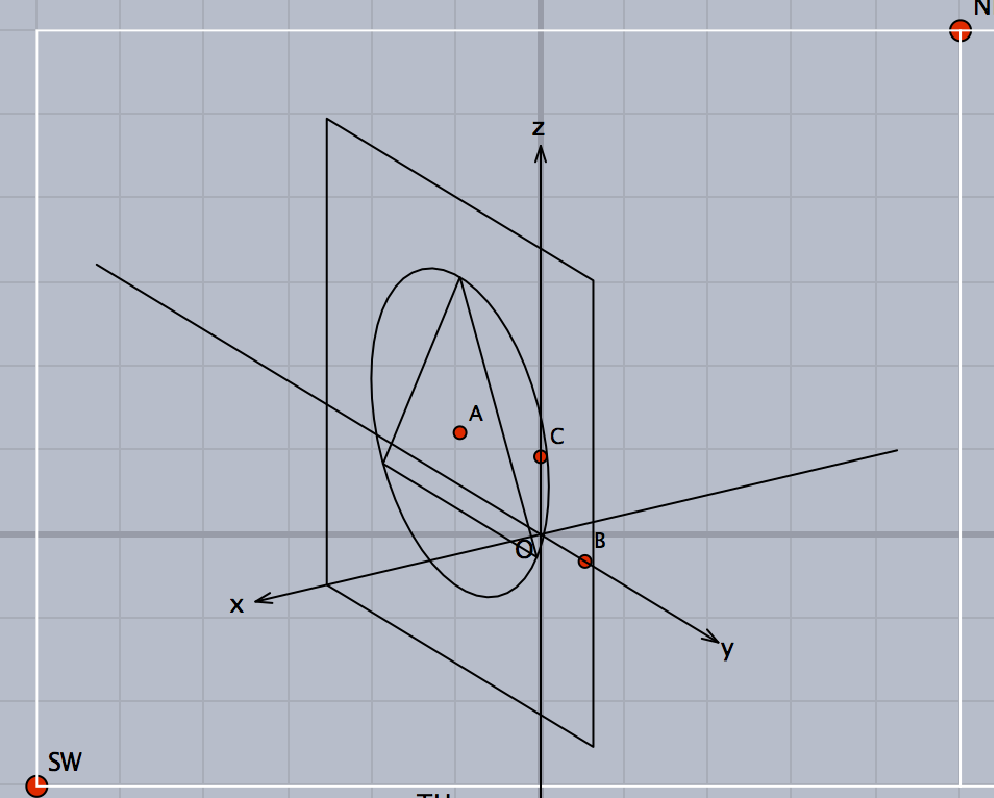
\includegraphics[bb=0 0 477.02 383.02 , width=6cm]{Fig/embed03.pdf}
\end{center}

この場合,点B,Cの座標がそのまま基本ベクトルとなっているが,原点Aに対して描画平面上にはB,Cがないので図がわかりにくい。図をわかりやすくするならば次のようにする。
\begin{verbatim}
  Putpoint3d(["A",[3,3,3],"B",[3,4,3],"C",[3,3,4]],"fix");
  Embed("1",["cr1","sg1"],"A3d+x*(B3d-A3d)+y*(C3d-A3d)","[x,y]");
\end{verbatim}

  また,平面を記述するのに,平面の原点と法線ベクトルを用いて Perpplane() を用いると,基本ベクトルが生成されるので、これを利用することができる。次のスクリプトでは,Skeletonparadata() を用いて陰線処理もしている。
\begin{verbatim}
  Xyzax3data("","x=[-5,5]","y=[-8,5]","z=[-5,5]");
  Putpoint3d(["O",[0,0,0],"P",[1,1,2]],"fix");
  Perpplane("E-F","P",P3d-O3d,"put");
  vec1=3*(E3d-P3d);
  vec2=3*(F3d-P3d);
  Putpoint3d(["A",P3d+vec1+vec2],"fix");
  Putpoint3d(["B",P3d+vec1-vec2],"fix");
  Putpoint3d(["C",P3d-vec1-vec2],"fix");
  Putpoint3d(["D",P3d-vec1+vec2],"fix");
  Spaceline("1",[A,B,C,D,A]);
  Circledata("1",[[0,0],[2,0]],["nodisp"]);
  Listplot("1",[[0,2],[-sqrt(3),-1],[sqrt(3),-1],[0,2]],["nodisp"]);
  Embed("1",["cr1","sg1"],"P3d+x*(E3d-P3d)+y*(F3d-P3d)","[x,y]");
  Ptsize(3);
  Drawpoint(P);
  Skeletonparadata("1");
\end{verbatim}
         \begin{center} %%% /Users/Hannya/ketcindy/ketwork/template.tex 2016-8-18 21:20
%%% template.sce 2016-8-18 21:20
{\unitlength=8mm%
\begin{picture}%
(   9.18000,   7.71000)(  -4.79000,  -2.03000)%
\special{pn 8}%
%
\settowidth{\Width}{$x$}\setlength{\Width}{-0.5\Width}%
\settoheight{\Height}{$x$}\settodepth{\Depth}{$x$}\setlength{\Height}{-0.5\Height}\setlength{\Depth}{0.5\Depth}\addtolength{\Height}{\Depth}%
\put(-4.4289,-1.0449){\hspace*{\Width}\raisebox{\Height}{$x$}}%
%
%
\settowidth{\Width}{$y$}\setlength{\Width}{-0.5\Width}%
\settoheight{\Height}{$y$}\settodepth{\Depth}{$y$}\setlength{\Height}{-0.5\Height}\setlength{\Depth}{0.5\Depth}\addtolength{\Height}{\Depth}%
\put(2.8060,-1.7060){\hspace*{\Width}\raisebox{\Height}{$y$}}%
%
%
\settowidth{\Width}{$z$}\setlength{\Width}{-0.5\Width}%
\settoheight{\Height}{$z$}\settodepth{\Depth}{$z$}\setlength{\Height}{-0.5\Height}\setlength{\Depth}{0.5\Depth}\addtolength{\Height}{\Depth}%
\put(0.0000,4.8175){\hspace*{\Width}\raisebox{\Height}{$z$}}%
%
%
\special{pn 3}%
\special{pa -92 -427}\special{pa -99 -430}\special{pa -106 -429}\special{pa -111 -424}%
\special{pa -112 -417}\special{pa -109 -410}\special{pa -103 -407}\special{pa -95 -408}%
\special{pa -90 -413}\special{pa -89 -421}\special{pa -92 -427}\special{sh 1}\special{fp}%
\special{pn 8}%
\special{pa 1337 -315}\special{pa 811 -191}%
\special{fp}%
\special{pa 758 -179}\special{pa 380 -90}%
\special{fp}%
\special{pa 305 -72}\special{pa -311 73}%
\special{fp}%
\special{pa -385 91}\special{pa -1166 275}%
\special{fp}%
\special{pa -1219 288}\special{pa -1337 315}%
\special{fp}%
\special{pa -1332 -810}\special{pa -1019 -619}%
\special{fp}%
\special{pa -976 -593}\special{pa -742 -451}%
\special{fp}%
\special{pa -697 -424}\special{pa -581 -353}%
\special{fp}%
\special{pa -538 -327}\special{pa -306 -186}%
\special{fp}%
\special{pa -238 -144}\special{pa 78 47}%
\special{fp}%
\special{pa 130 79}\special{pa 635 386}%
\special{fp}%
\special{pa 677 412}\special{pa 833 506}%
\special{fp}%
\special{pa 0 639}\special{pa 0 418}%
\special{fp}%
\special{pa 0 369}\special{pa 0 119}%
\special{fp}%
\special{pa 0 68}\special{pa 0 -117}%
\special{fp}%
\special{pa 0 -166}\special{pa 0 -1458}%
\special{fp}%
\special{pa 993 -1126}\special{pa 645 451}\special{pa -1195 289}\special{pa -846 -1288}%
\special{pa -24 -1216}%
\special{fp}%
\special{pa 24 -1212}\special{pa 993 -1126}%
\special{fp}%
\special{pa 513 -365}\special{pa 523 -431}\special{pa 522 -497}\special{pa 513 -562}%
\special{pa 493 -625}\special{pa 464 -684}\special{pa 426 -740}\special{pa 380 -790}%
\special{pa 326 -834}\special{pa 266 -872}\special{pa 199 -903}\special{pa 129 -926}%
\special{pa 54 -941}\special{pa 24 -943}%
\special{fp}%
\special{pa -24 -947}\special{pa -101 -946}\special{pa -180 -936}\special{pa -257 -918}%
\special{pa -331 -892}\special{pa -402 -859}\special{pa -468 -818}\special{pa -529 -772}%
\special{pa -582 -720}\special{pa -628 -663}\special{pa -666 -602}\special{pa -695 -538}%
\special{pa -714 -473}\special{pa -724 -406}\special{pa -724 -340}\special{pa -714 -275}%
\special{pa -695 -212}\special{pa -666 -153}\special{pa -628 -98}\special{pa -582 -48}%
\special{pa -528 -3}\special{pa -467 35}\special{pa -401 65}\special{pa -330 88}\special{pa -255 103}%
\special{pa -178 110}\special{pa -100 108}\special{pa -22 99}\special{pa 55 81}\special{pa 130 55}%
\special{pa 201 21}\special{pa 267 -19}\special{pa 327 -66}\special{pa 381 -118}\special{pa 427 -175}%
\special{pa 465 -235}\special{pa 493 -299}\special{pa 513 -365}%
\special{fp}%
\special{pa -22 -905}\special{pa -690 -202}\special{pa 372 -109}\special{pa 16 -945}%
\special{fp}%
\end{picture}}% \end{center}

\begin{flushright} \hyperlink{functionlist}{$\Rightarrow$関数一覧}\end{flushright}


\hypertarget{intersectcrvsf}{}
\item[関数]  Intersectcrvsf(name,PD,式)
\item[機能]  曲線と曲面の交点の座標を求める
\item[説明]  PDは曲線のプロットデータ。式は曲面の式。

  曲面は,Sfbdparadata()でデータを作成し,ExeccmdC()で表示しておく。交点の座標は,"intercrvsf"+name に代入される。コマンドの実行順序は次の例のようにする。

\vspace{\baselineskip}
【例】回転放物面と線分の交点の座標を表示する。
\begin{verbatim}
    Putpoint3d(["A",[0,-3,0],"B",[0,3,2]],"fix");
    Spaceline("1",[A,B]);
    fd=[
     "z=4-(x^2+y^2)","x=R*cos(T)","y=R*sin(T)",
     "R=[0,2]","T=[0,2*pi]","e"
    ];
    Startsurf();
    Sfbdparadata("1",fd);
    Intersectcrvsf("1","sl3d1",fd);
    ExeccmdC("1",[""]);
    println("Intersect="+intercrvsf1);
    Drawpoint3d(intercrvsf1); 
\end{verbatim}
実行すると,コンソールに\\
    \verb|Intersect=[[0,1.57,1.52],[0,-1.91,0.36]] |
と表示され,画面には緑で交点が表示される。。


\vspace{\baselineskip}
\hypertarget{intersectsgpL}{}
\item[関数]  IntersectsgpL(点名,線分,面,描画方法)
\item[機能]  空間の線分(直線)と平面の交点を求める。
\item[説明]  引数の線分は線分の端点を "A-B" の形もしくは空間座標のリストで与える。

  引数の面は,面内の3点を "C-D-E" の形もしくは空間座標のリストで与える。

  戻り値は,[pt,flag1,flag2,val1,val2]
  
  pt:直線と平面の交点の座標。直線と平面が平行で交点が存在しない場合は空リスト[]
  
  flag1 : 交点が線分内にあれば true ,なければ false
  
  flag2 : 交点が面内にあれば true,なければ false
  
  val1,val2 : 
  
  描画方法は,"put" または "i" , "e" 。
  
  put : 幾何点を作る

   i : 線分内にあれば点を描く

 e :  平面で交われば点を描く
  
\vspace{\baselineskip}
【例】座標のリストで与える記述例\\
  \verb|IntersectsgpL("P",[p1,p2],[p3,p4,p5],"draw");| 
  
\vspace{\baselineskip}
【例】立方体を平面で切った図を描く。

   いろいろな手順が考えられるが,ここでは次の手順で描く。
   
 (1) 立方体の頂点をとる。1辺の長さをHnとする。
 
    ここでは軸上の点はPutaxes3d()でとる。
    
(2) 切断面を決める点E,F,Gを辺上の自由点としてPutonseg3d()でとる。

(3) E,F,Gを通る平面と,辺AC,DYとの交点をとり,M,Nとする。

(4) 全体を多面体として面データを作って描画する。
\begin{verbatim}
  Hn=3;
  Putaxes3d(Hn);
  Putpoint3d("A",[Hn,Hn,0],"fix");
  Putpoint3d("B",[Hn,0,Hn],"fix");
  Putpoint3d("C",[Hn,Hn,Hn],"fix");
  Putpoint3d("D",[0,Hn,Hn],"fix");
  Putonseg3d("E",X,B); 
  Putonseg3d("F",Z,B); 
  Putonseg3d("G",Z,D); 
  IntersectsgpL("M","A-C","E-F-G","put"); 
  IntersectsgpL("N","D-Y","E-F-G","put"); 
  phd=Concatobj([[O,X,A,Y],[X,A,M,E],[A,Y,N,M],[Y,N,G,Z,O],
      [O,Z,F,E,X],[Z,F,G],[E,M,N,G,F]]);
  VertexEdgeFace("1",phd,["Edg=nogeo"]);
  Nohiddenbyfaces("1","phf3d1"); 
\end{verbatim}
Cinderellaの描画面はつぎのようになる。点E,F,Gをドラッグして,適当な位置の断面にする。ただし,M,Nは辺上にあることが条件である。

\vspace{\baselineskip}
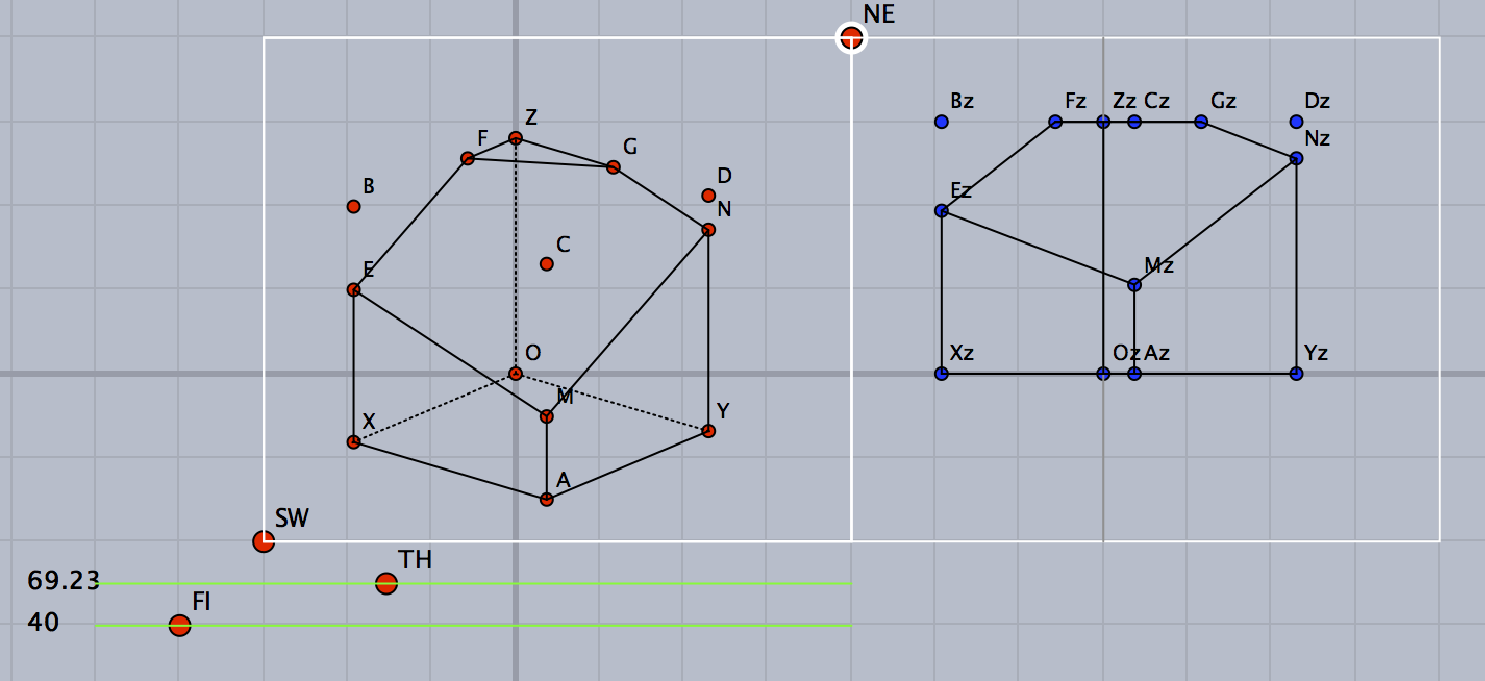
\includegraphics[bb=0 0 713.04 327.02 , width=12cm]{Fig/IntersectsgpL0.pdf}


できた図は下図左。これに,次のスクリプトを追加すれば,断面上方の立方体の各辺も点線で描かれる。(下図右)
\begin{verbatim}
  Spaceline("1",[E,B,F],["do"]);
  Spaceline("2",[B,C,M],["do"]);
  Spaceline("3",[C,D,N],["do"]);
  Spaceline("4",[D,G],["do"]);
\end{verbatim}
\begin{center} %%% /Users/Hannya/ketcindy/ketwork/template.tex 2016-8-9 13:39
%%% template.sce 2016-8-9 13:39
{\unitlength=8mm%
\begin{picture}%
(   7.00000,   6.00000)(  -3.00000,  -2.00000)%
\special{pn 8}%
%
\special{pn 8}%
\special{pa 4 -2}\special{pa -4 2}\special{fp}\special{pa -32 14}\special{pa -39 17}\special{fp}%
\special{pa -68 29}\special{pa -75 32}\special{fp}\special{pa -103 44}\special{pa -111 47}\special{fp}%
\special{pa -139 59}\special{pa -147 62}\special{fp}\special{pa -175 74}\special{pa -182 77}\special{fp}%
\special{pa -211 89}\special{pa -218 92}\special{fp}\special{pa -246 104}\special{pa -254 107}\special{fp}%
\special{pa -282 119}\special{pa -290 122}\special{fp}\special{pa -318 134}\special{pa -325 137}\special{fp}%
\special{pa -354 149}\special{pa -361 153}\special{fp}\special{pa -389 164}\special{pa -397 168}\special{fp}%
\special{pa -425 180}\special{pa -432 183}\special{fp}\special{pa -461 195}\special{pa -468 198}\special{fp}%
\special{pa -496 210}\special{pa -504 213}\special{fp}\special{pa -532 225}\special{pa -540 228}\special{fp}%
\special{pa -568 240}\special{pa -575 243}\special{fp}\special{pa -604 255}\special{pa -611 258}\special{fp}%
\special{pn 8}%
\special{pa -607 257}\special{pa 116 472}%
\special{fp}%
\special{pa 116 472}\special{pa 724 215}%
\special{fp}%
\special{pn 8}%
\special{pa -4 -1}\special{pa 4 1}\special{fp}\special{pa 34 10}\special{pa 42 12}\special{fp}%
\special{pa 72 22}\special{pa 80 24}\special{fp}\special{pa 110 33}\special{pa 118 35}\special{fp}%
\special{pa 149 44}\special{pa 156 46}\special{fp}\special{pa 187 56}\special{pa 194 58}\special{fp}%
\special{pa 225 67}\special{pa 232 69}\special{fp}\special{pa 263 78}\special{pa 271 80}\special{fp}%
\special{pa 301 90}\special{pa 309 92}\special{fp}\special{pa 339 101}\special{pa 347 103}\special{fp}%
\special{pa 377 112}\special{pa 385 114}\special{fp}\special{pa 415 124}\special{pa 423 126}\special{fp}%
\special{pa 453 135}\special{pa 461 137}\special{fp}\special{pa 491 146}\special{pa 499 148}\special{fp}%
\special{pa 530 158}\special{pa 537 160}\special{fp}\special{pa 568 169}\special{pa 575 171}\special{fp}%
\special{pa 606 180}\special{pa 613 182}\special{fp}\special{pa 644 192}\special{pa 651 194}\special{fp}%
\special{pa 682 203}\special{pa 690 205}\special{fp}\special{pa 720 214}\special{pa 728 216}\special{fp}%
\special{pn 8}%
\special{pa 116 472}\special{pa 116 160}%
\special{fp}%
\special{pa 116 160}\special{pa -607 -315}%
\special{fp}%
\special{pa -607 257}\special{pa -607 -315}%
\special{fp}%
\special{pa 724 215}\special{pa 724 -539}%
\special{fp}%
\special{pa 116 160}\special{pa 724 -539}%
\special{fp}%
\special{pa 724 -539}\special{pa 367 -774}%
\special{fp}%
\special{pa 367 -774}\special{pa 0 -883}%
\special{fp}%
\special{pn 8}%
\special{pa 0 4}\special{pa 0 -4}\special{fp}\special{pa 0 -36}\special{pa 0 -44}\special{fp}%
\special{pa 0 -76}\special{pa 0 -84}\special{fp}\special{pa 0 -116}\special{pa 0 -124}\special{fp}%
\special{pa 0 -157}\special{pa 0 -165}\special{fp}\special{pa 0 -197}\special{pa 0 -205}\special{fp}%
\special{pa 0 -237}\special{pa 0 -245}\special{fp}\special{pa 0 -277}\special{pa 0 -285}\special{fp}%
\special{pa 0 -317}\special{pa 0 -325}\special{fp}\special{pa 0 -357}\special{pa 0 -365}\special{fp}%
\special{pa 0 -398}\special{pa 0 -406}\special{fp}\special{pa 0 -438}\special{pa 0 -446}\special{fp}%
\special{pa 0 -478}\special{pa 0 -486}\special{fp}\special{pa 0 -518}\special{pa 0 -526}\special{fp}%
\special{pa 0 -558}\special{pa 0 -566}\special{fp}\special{pa 0 -598}\special{pa 0 -606}\special{fp}%
\special{pa 0 -639}\special{pa 0 -647}\special{fp}\special{pa 0 -679}\special{pa 0 -687}\special{fp}%
\special{pa 0 -719}\special{pa 0 -727}\special{fp}\special{pa 0 -759}\special{pa 0 -767}\special{fp}%
\special{pa 0 -799}\special{pa 0 -807}\special{fp}\special{pa 0 -839}\special{pa 0 -847}\special{fp}%
\special{pa 0 -879}\special{pa 0 -887}\special{fp}\special{pn 8}%
\special{pa 0 -883}\special{pa -180 -807}%
\special{fp}%
\special{pa -607 -315}\special{pa -180 -807}%
\special{fp}%
\special{pa 367 -774}\special{pa -180 -807}%
\special{fp}%
\end{picture}}%    %%% /Users/Hannya/ketcindy/ketwork/template.tex 2016-8-9 13:37
%%% template.sce 2016-8-9 13:37
{\unitlength=8mm%
\begin{picture}%
(   7.00000,   6.00000)(  -3.00000,  -2.00000)%
\special{pn 8}%
%
\special{pn 8}%
\special{pa 4 -2}\special{pa -4 2}\special{fp}\special{pa -32 14}\special{pa -39 17}\special{fp}%
\special{pa -68 29}\special{pa -75 32}\special{fp}\special{pa -103 44}\special{pa -111 47}\special{fp}%
\special{pa -139 59}\special{pa -147 62}\special{fp}\special{pa -175 74}\special{pa -182 77}\special{fp}%
\special{pa -211 89}\special{pa -218 92}\special{fp}\special{pa -246 104}\special{pa -254 107}\special{fp}%
\special{pa -282 119}\special{pa -290 122}\special{fp}\special{pa -318 134}\special{pa -325 137}\special{fp}%
\special{pa -354 149}\special{pa -361 153}\special{fp}\special{pa -389 164}\special{pa -397 168}\special{fp}%
\special{pa -425 180}\special{pa -432 183}\special{fp}\special{pa -461 195}\special{pa -468 198}\special{fp}%
\special{pa -496 210}\special{pa -504 213}\special{fp}\special{pa -532 225}\special{pa -540 228}\special{fp}%
\special{pa -568 240}\special{pa -575 243}\special{fp}\special{pa -604 255}\special{pa -611 258}\special{fp}%
\special{pn 8}%
\special{pa -607 257}\special{pa 116 472}%
\special{fp}%
\special{pa 116 472}\special{pa 724 215}%
\special{fp}%
\special{pn 8}%
\special{pa -4 -1}\special{pa 4 1}\special{fp}\special{pa 34 10}\special{pa 42 12}\special{fp}%
\special{pa 72 22}\special{pa 80 24}\special{fp}\special{pa 110 33}\special{pa 118 35}\special{fp}%
\special{pa 149 44}\special{pa 156 46}\special{fp}\special{pa 187 56}\special{pa 194 58}\special{fp}%
\special{pa 225 67}\special{pa 232 69}\special{fp}\special{pa 263 78}\special{pa 271 80}\special{fp}%
\special{pa 301 90}\special{pa 309 92}\special{fp}\special{pa 339 101}\special{pa 347 103}\special{fp}%
\special{pa 377 112}\special{pa 385 114}\special{fp}\special{pa 415 124}\special{pa 423 126}\special{fp}%
\special{pa 453 135}\special{pa 461 137}\special{fp}\special{pa 491 146}\special{pa 499 148}\special{fp}%
\special{pa 530 158}\special{pa 537 160}\special{fp}\special{pa 568 169}\special{pa 575 171}\special{fp}%
\special{pa 606 180}\special{pa 613 182}\special{fp}\special{pa 644 192}\special{pa 651 194}\special{fp}%
\special{pa 682 203}\special{pa 690 205}\special{fp}\special{pa 720 214}\special{pa 728 216}\special{fp}%
\special{pn 8}%
\special{pa 116 472}\special{pa 116 160}%
\special{fp}%
\special{pa 116 160}\special{pa -607 -315}%
\special{fp}%
\special{pa -607 257}\special{pa -607 -315}%
\special{fp}%
\special{pa 724 215}\special{pa 724 -539}%
\special{fp}%
\special{pa 116 160}\special{pa 724 -539}%
\special{fp}%
\special{pa 724 -539}\special{pa 367 -774}%
\special{fp}%
\special{pa 367 -774}\special{pa 0 -883}%
\special{fp}%
\special{pn 8}%
\special{pa 0 4}\special{pa 0 -4}\special{fp}\special{pa 0 -36}\special{pa 0 -44}\special{fp}%
\special{pa 0 -76}\special{pa 0 -84}\special{fp}\special{pa 0 -116}\special{pa 0 -124}\special{fp}%
\special{pa 0 -157}\special{pa 0 -165}\special{fp}\special{pa 0 -197}\special{pa 0 -205}\special{fp}%
\special{pa 0 -237}\special{pa 0 -245}\special{fp}\special{pa 0 -277}\special{pa 0 -285}\special{fp}%
\special{pa 0 -317}\special{pa 0 -325}\special{fp}\special{pa 0 -357}\special{pa 0 -365}\special{fp}%
\special{pa 0 -398}\special{pa 0 -406}\special{fp}\special{pa 0 -438}\special{pa 0 -446}\special{fp}%
\special{pa 0 -478}\special{pa 0 -486}\special{fp}\special{pa 0 -518}\special{pa 0 -526}\special{fp}%
\special{pa 0 -558}\special{pa 0 -566}\special{fp}\special{pa 0 -598}\special{pa 0 -606}\special{fp}%
\special{pa 0 -639}\special{pa 0 -647}\special{fp}\special{pa 0 -679}\special{pa 0 -687}\special{fp}%
\special{pa 0 -719}\special{pa 0 -727}\special{fp}\special{pa 0 -759}\special{pa 0 -767}\special{fp}%
\special{pa 0 -799}\special{pa 0 -807}\special{fp}\special{pa 0 -839}\special{pa 0 -847}\special{fp}%
\special{pa 0 -879}\special{pa 0 -887}\special{fp}\special{pn 8}%
\special{pa 0 -883}\special{pa -180 -807}%
\special{fp}%
\special{pa -607 -315}\special{pa -180 -807}%
\special{fp}%
\special{pa 367 -774}\special{pa -180 -807}%
\special{fp}%
\special{pn 8}%
\special{pa -607 -311}\special{pa -607 -319}\special{fp}\special{pa -607 -349}\special{pa -607 -357}\special{fp}%
\special{pa -607 -388}\special{pa -607 -396}\special{fp}\special{pa -607 -427}\special{pa -607 -435}\special{fp}%
\special{pa -607 -466}\special{pa -607 -474}\special{fp}\special{pa -607 -505}\special{pa -607 -513}\special{fp}%
\special{pa -607 -543}\special{pa -607 -551}\special{fp}\special{pa -607 -582}\special{pa -607 -590}\special{fp}%
\special{pa -609 -622}\special{pa -605 -628}\special{fp}\special{pa -577 -640}\special{pa -570 -643}\special{fp}%
\special{pa -541 -655}\special{pa -534 -658}\special{fp}\special{pa -505 -670}\special{pa -498 -673}\special{fp}%
\special{pa -470 -685}\special{pa -462 -688}\special{fp}\special{pa -434 -700}\special{pa -427 -703}\special{fp}%
\special{pa -398 -715}\special{pa -391 -718}\special{fp}\special{pa -363 -730}\special{pa -355 -733}\special{fp}%
\special{pa -327 -745}\special{pa -319 -749}\special{fp}\special{pa -291 -761}\special{pa -284 -764}\special{fp}%
\special{pa -255 -776}\special{pa -248 -779}\special{fp}\special{pa -220 -791}\special{pa -212 -794}\special{fp}%
\special{pa -184 -806}\special{pa -176 -809}\special{fp}\special{pn 8}%
\special{pn 8}%
\special{pa -611 -628}\special{pa -604 -626}\special{fp}\special{pa -574 -617}\special{pa -566 -615}\special{fp}%
\special{pa -536 -606}\special{pa -529 -603}\special{fp}\special{pa -499 -595}\special{pa -491 -592}\special{fp}%
\special{pa -462 -584}\special{pa -454 -581}\special{fp}\special{pa -424 -572}\special{pa -417 -570}\special{fp}%
\special{pa -387 -561}\special{pa -379 -559}\special{fp}\special{pa -349 -550}\special{pa -342 -548}\special{fp}%
\special{pa -312 -539}\special{pa -304 -537}\special{fp}\special{pa -275 -528}\special{pa -267 -526}\special{fp}%
\special{pa -237 -517}\special{pa -230 -514}\special{fp}\special{pa -200 -506}\special{pa -192 -503}\special{fp}%
\special{pa -162 -495}\special{pa -155 -492}\special{fp}\special{pa -125 -483}\special{pa -117 -481}\special{fp}%
\special{pa -88 -472}\special{pa -80 -470}\special{fp}\special{pa -50 -461}\special{pa -43 -459}\special{fp}%
\special{pa -13 -450}\special{pa -5 -448}\special{fp}\special{pa 25 -439}\special{pa 32 -437}\special{fp}%
\special{pa 62 -428}\special{pa 70 -425}\special{fp}\special{pa 100 -418}\special{pa 106 -413}\special{fp}%
\special{pa 116 -390}\special{pa 117 -382}\special{fp}\special{pa 116 -351}\special{pa 116 -343}\special{fp}%
\special{pa 116 -312}\special{pa 116 -304}\special{fp}\special{pa 116 -273}\special{pa 116 -265}\special{fp}%
\special{pa 116 -234}\special{pa 116 -226}\special{fp}\special{pa 116 -195}\special{pa 116 -187}\special{fp}%
\special{pa 116 -156}\special{pa 116 -148}\special{fp}\special{pa 116 -117}\special{pa 116 -109}\special{fp}%
\special{pa 116 -78}\special{pa 116 -70}\special{fp}\special{pa 116 -39}\special{pa 116 -31}\special{fp}%
\special{pa 116 0}\special{pa 116 8}\special{fp}\special{pa 116 39}\special{pa 116 47}\special{fp}%
\special{pa 116 78}\special{pa 116 86}\special{fp}\special{pa 116 117}\special{pa 116 125}\special{fp}%
\special{pa 116 156}\special{pa 116 164}\special{fp}\special{pn 8}%
\special{pn 8}%
\special{pa 113 -410}\special{pa 120 -413}\special{fp}\special{pa 149 -425}\special{pa 156 -428}\special{fp}%
\special{pa 185 -441}\special{pa 193 -444}\special{fp}\special{pa 222 -456}\special{pa 229 -459}\special{fp}%
\special{pa 258 -471}\special{pa 265 -474}\special{fp}\special{pa 294 -487}\special{pa 302 -490}\special{fp}%
\special{pa 331 -502}\special{pa 338 -505}\special{fp}\special{pa 367 -517}\special{pa 374 -521}\special{fp}%
\special{pa 403 -533}\special{pa 411 -536}\special{fp}\special{pa 440 -548}\special{pa 447 -551}\special{fp}%
\special{pa 476 -564}\special{pa 484 -567}\special{fp}\special{pa 512 -579}\special{pa 520 -582}\special{fp}%
\special{pa 549 -594}\special{pa 556 -597}\special{fp}\special{pa 585 -610}\special{pa 593 -613}\special{fp}%
\special{pa 621 -625}\special{pa 629 -628}\special{fp}\special{pa 658 -640}\special{pa 665 -643}\special{fp}%
\special{pa 694 -656}\special{pa 702 -658}\special{fp}\special{pa 721 -660}\special{pa 727 -654}\special{fp}%
\special{pa 724 -621}\special{pa 724 -613}\special{fp}\special{pa 724 -582}\special{pa 724 -574}\special{fp}%
\special{pa 724 -543}\special{pa 724 -535}\special{fp}\special{pn 8}%
\special{pn 8}%
\special{pa 728 -667}\special{pa 720 -669}\special{fp}\special{pa 688 -679}\special{pa 680 -681}\special{fp}%
\special{pa 648 -691}\special{pa 641 -693}\special{fp}\special{pa 609 -702}\special{pa 601 -705}\special{fp}%
\special{pa 569 -714}\special{pa 561 -717}\special{fp}\special{pa 529 -726}\special{pa 522 -728}\special{fp}%
\special{pa 490 -738}\special{pa 482 -740}\special{fp}\special{pa 450 -750}\special{pa 442 -752}\special{fp}%
\special{pa 410 -761}\special{pa 403 -764}\special{fp}\special{pa 371 -773}\special{pa 363 -776}\special{fp}%
\special{pn 8}%
\end{picture}}% \end{center}

\begin{flushright} \hyperlink{functionlist}{$\Rightarrow$関数一覧}\end{flushright}

\hypertarget{invparapt}{}
\item[関数]  Invparapt(座標,PD)
\item[機能]  描画面上の座標に対応する曲線上の点の座標を返す
\item[説明]  Cinderellaの描画面上の座標を与えて,それに対応する曲線上の3次元座標を返す。
\\
空間内の曲線を作図すると,曲線の空間内のプロットデータとともに,描画面上に描くためのプロットデータも作られる。これを利用すると,描画面上の位置から曲線上の座標を求めることができる。

\vspace{\baselineskip}
【例】螺旋と線分を描いたとき,描画面上での交点(空間内の交点ではない)に対応する螺旋上の点の座標を求め部分曲線を描く。

\begin{verbatim}
  Spaceline("1",[[-1,-1,-1],[1,2,3]]);
  Spacecurve("1","[2*cos(t),2*sin(t),0.2*t]","t=[0,4*pi]",["do"]);
  tmp=Intersectcrvs("sl2d1","sc2d1");
  p1=Invparapt(tmp_1,"sc3d1");
  p2=Invparapt(tmp_2,"sc3d1");
  Partcrv3d("1",p1,p2,"sc3d1"); 
\end{verbatim}
 \begin{center}\scalebox{0.8}{ %%% /Users/Hannya/ketcindy/ketwork/template.tex 2016-8-23 9:12
%%% template.sce 2016-8-23 9:12
{\unitlength=8mm%
\begin{picture}%
(   7.55000,   6.27000)(  -3.75000,  -1.85000)%
\special{pn 8}%
%
\settowidth{\Width}{$x$}\setlength{\Width}{-0.5\Width}%
\settoheight{\Height}{$x$}\settodepth{\Depth}{$x$}\setlength{\Height}{-0.5\Height}\setlength{\Depth}{0.5\Depth}\addtolength{\Height}{\Depth}%
\put(-3.1557,-0.9707){\hspace*{\Width}\raisebox{\Height}{$x$}}%
%
%
\settowidth{\Width}{$y$}\setlength{\Width}{-0.5\Width}%
\settoheight{\Height}{$y$}\settodepth{\Depth}{$y$}\setlength{\Height}{-0.5\Height}\setlength{\Depth}{0.5\Depth}\addtolength{\Height}{\Depth}%
\put(3.5211,-1.3391){\hspace*{\Width}\raisebox{\Height}{$y$}}%
%
%
\settowidth{\Width}{$z$}\setlength{\Width}{-0.5\Width}%
\settoheight{\Height}{$z$}\settodepth{\Depth}{$z$}\setlength{\Height}{-0.5\Height}\setlength{\Depth}{0.5\Depth}\addtolength{\Height}{\Depth}%
\put(0.0000,3.9488){\hspace*{\Width}\raisebox{\Height}{$z$}}%
%
%
\special{pa 1171 -360}\special{pa -937 288}%
\special{fp}%
\special{pa -1053 -400}\special{pa 1053 400}%
\special{fp}%
\special{pa 0 583}\special{pa 0 -1184}%
\special{fp}%
\special{pa 24 144}\special{pa 187 -656}%
\special{fp}%
\special{pn 8}%
\special{pa -472 143}\special{pa -464 145}\special{fp}\special{pa -434 150}\special{pa -426 151}\special{fp}%
\special{pa -395 157}\special{pa -387 158}\special{fp}\special{pa -356 163}\special{pa -348 164}\special{fp}%
\special{pa -317 167}\special{pa -309 167}\special{fp}\special{pa -278 169}\special{pa -270 170}\special{fp}%
\special{pa -239 172}\special{pa -231 172}\special{fp}\special{pa -199 173}\special{pa -191 173}\special{fp}%
\special{pa -160 173}\special{pa -152 172}\special{fp}\special{pa -121 172}\special{pa -113 171}\special{fp}%
\special{pa -82 171}\special{pa -74 170}\special{fp}\special{pa -42 169}\special{pa -34 168}\special{fp}%
\special{pa -3 165}\special{pa 5 164}\special{fp}\special{pa 36 160}\special{pa 44 160}\special{fp}%
\special{pa 75 156}\special{pa 83 155}\special{fp}\special{pa 114 151}\special{pa 122 150}\special{fp}%
\special{pa 152 143}\special{pa 160 142}\special{fp}\special{pa 191 136}\special{pa 199 134}\special{fp}%
\special{pa 229 128}\special{pa 237 126}\special{fp}\special{pa 267 119}\special{pa 275 117}\special{fp}%
\special{pa 305 107}\special{pa 312 105}\special{fp}\special{pa 342 95}\special{pa 350 93}\special{fp}%
\special{pa 380 83}\special{pa 387 81}\special{fp}\special{pa 416 68}\special{pa 423 64}\special{fp}%
\special{pa 451 51}\special{pa 458 47}\special{fp}\special{pa 487 34}\special{pa 493 30}\special{fp}%
\special{pa 519 12}\special{pa 526 8}\special{fp}\special{pa 550 -12}\special{pa 556 -17}\special{fp}%
\special{pa 581 -36}\special{pa 586 -42}\special{fp}\special{pa 602 -69}\special{pa 606 -76}\special{fp}%
\special{pa 622 -103}\special{pa 624 -110}\special{fp}\special{pa 625 -142}\special{pa 625 -150}\special{fp}%
\special{pa 621 -179}\special{pa 619 -187}\special{fp}\special{pa 604 -215}\special{pa 599 -221}\special{fp}%
\special{pa 581 -246}\special{pa 576 -252}\special{fp}\special{pa 552 -272}\special{pa 546 -277}\special{fp}%
\special{pa 522 -298}\special{pa 516 -302}\special{fp}\special{pa 488 -317}\special{pa 481 -321}\special{fp}%
\special{pa 453 -335}\special{pa 446 -339}\special{fp}\special{pa 418 -353}\special{pa 411 -357}\special{fp}%
\special{pa 381 -367}\special{pa 374 -369}\special{fp}\special{pa 344 -379}\special{pa 337 -382}\special{fp}%
\special{pa 307 -392}\special{pa 300 -395}\special{fp}\special{pa 270 -403}\special{pa 262 -405}\special{fp}%
\special{pa 231 -412}\special{pa 223 -414}\special{fp}\special{pa 193 -420}\special{pa 185 -422}\special{fp}%
\special{pa 155 -429}\special{pa 147 -430}\special{fp}\special{pa 116 -436}\special{pa 108 -437}\special{fp}%
\special{pa 77 -441}\special{pa 69 -442}\special{fp}\special{pa 38 -445}\special{pa 30 -446}\special{fp}%
\special{pa -1 -450}\special{pa -9 -451}\special{fp}\special{pa -40 -454}\special{pa -48 -454}\special{fp}%
\special{pa -79 -455}\special{pa -87 -456}\special{fp}\special{pa -119 -457}\special{pa -127 -457}\special{fp}%
\special{pa -158 -458}\special{pa -166 -459}\special{fp}\special{pa -197 -458}\special{pa -205 -458}\special{fp}%
\special{pa -236 -457}\special{pa -244 -456}\special{fp}\special{pa -276 -455}\special{pa -284 -454}\special{fp}%
\special{pa -315 -453}\special{pa -323 -452}\special{fp}\special{pa -354 -448}\special{pa -362 -447}\special{fp}%
\special{pa -393 -442}\special{pa -401 -441}\special{fp}\special{pa -432 -436}\special{pa -439 -435}\special{fp}%
\special{pa -470 -428}\special{pa -477 -425}\special{fp}\special{pa -507 -417}\special{pa -515 -414}\special{fp}%
\special{pa -545 -405}\special{pa -552 -402}\special{fp}\special{pa -579 -386}\special{pa -586 -382}\special{fp}%
\special{pa -610 -364}\special{pa -615 -357}\special{fp}\special{pa -627 -330}\special{pa -627 -322}\special{fp}%
\special{pa -613 -294}\special{pa -608 -288}\special{fp}\special{pa -581 -272}\special{pa -574 -268}\special{fp}%
\special{pa -547 -254}\special{pa -539 -251}\special{fp}\special{pa -509 -241}\special{pa -502 -239}\special{fp}%
\special{pa -472 -229}\special{pa -464 -227}\special{fp}\special{pa -434 -222}\special{pa -426 -221}\special{fp}%
\special{pa -395 -215}\special{pa -387 -214}\special{fp}\special{pa -356 -208}\special{pa -348 -208}\special{fp}%
\special{pa -317 -205}\special{pa -309 -205}\special{fp}\special{pa -278 -203}\special{pa -270 -202}\special{fp}%
\special{pa -239 -200}\special{pa -231 -200}\special{fp}\special{pa -199 -199}\special{pa -191 -199}\special{fp}%
\special{pa -160 -199}\special{pa -152 -200}\special{fp}\special{pa -121 -200}\special{pa -113 -200}\special{fp}%
\special{pa -82 -201}\special{pa -74 -201}\special{fp}\special{pa -42 -203}\special{pa -34 -204}\special{fp}%
\special{pa -3 -207}\special{pa 5 -208}\special{fp}\special{pa 36 -211}\special{pa 44 -212}\special{fp}%
\special{pa 75 -216}\special{pa 83 -217}\special{fp}\special{pa 114 -221}\special{pa 122 -222}\special{fp}%
\special{pa 152 -229}\special{pa 160 -230}\special{fp}\special{pa 191 -236}\special{pa 199 -238}\special{fp}%
\special{pa 229 -244}\special{pa 237 -246}\special{fp}\special{pa 267 -253}\special{pa 275 -255}\special{fp}%
\special{pa 305 -265}\special{pa 312 -267}\special{fp}\special{pa 342 -277}\special{pa 350 -279}\special{fp}%
\special{pa 380 -288}\special{pa 387 -291}\special{fp}\special{pa 416 -304}\special{pa 423 -308}\special{fp}%
\special{pa 451 -321}\special{pa 458 -325}\special{fp}\special{pa 487 -338}\special{pa 493 -342}\special{fp}%
\special{pa 519 -360}\special{pa 526 -364}\special{fp}\special{pa 550 -384}\special{pa 556 -389}\special{fp}%
\special{pa 581 -408}\special{pa 586 -414}\special{fp}\special{pa 602 -441}\special{pa 606 -448}\special{fp}%
\special{pa 622 -474}\special{pa 624 -482}\special{fp}\special{pa 625 -514}\special{pa 625 -522}\special{fp}%
\special{pa 621 -551}\special{pa 619 -559}\special{fp}\special{pa 604 -586}\special{pa 599 -593}\special{fp}%
\special{pa 581 -618}\special{pa 576 -624}\special{fp}\special{pa 552 -644}\special{pa 546 -649}\special{fp}%
\special{pa 522 -670}\special{pa 516 -674}\special{fp}\special{pa 488 -689}\special{pa 481 -692}\special{fp}%
\special{pa 453 -707}\special{pa 446 -711}\special{fp}\special{pa 418 -725}\special{pa 411 -728}\special{fp}%
\special{pa 381 -739}\special{pa 374 -741}\special{fp}\special{pa 344 -751}\special{pa 337 -754}\special{fp}%
\special{pa 307 -764}\special{pa 300 -767}\special{fp}\special{pa 270 -775}\special{pa 262 -777}\special{fp}%
\special{pa 231 -784}\special{pa 223 -786}\special{fp}\special{pa 193 -792}\special{pa 185 -794}\special{fp}%
\special{pa 155 -801}\special{pa 147 -802}\special{fp}\special{pa 116 -808}\special{pa 108 -809}\special{fp}%
\special{pa 77 -813}\special{pa 69 -813}\special{fp}\special{pa 38 -817}\special{pa 30 -818}\special{fp}%
\special{pa -1 -822}\special{pa -9 -823}\special{fp}\special{pa -40 -826}\special{pa -48 -826}\special{fp}%
\special{pa -79 -827}\special{pa -87 -828}\special{fp}\special{pa -119 -829}\special{pa -127 -829}\special{fp}%
\special{pa -158 -830}\special{pa -166 -830}\special{fp}\special{pa -197 -830}\special{pa -205 -830}\special{fp}%
\special{pa -236 -828}\special{pa -244 -828}\special{fp}\special{pa -276 -827}\special{pa -284 -826}\special{fp}%
\special{pa -315 -825}\special{pa -323 -824}\special{fp}\special{pa -354 -820}\special{pa -362 -819}\special{fp}%
\special{pa -393 -814}\special{pa -401 -813}\special{fp}\special{pa -432 -808}\special{pa -439 -807}\special{fp}%
\special{pa -470 -799}\special{pa -477 -797}\special{fp}\special{pa -507 -789}\special{pa -515 -786}\special{fp}%
\special{pa -545 -777}\special{pa -552 -774}\special{fp}\special{pa -579 -758}\special{pa -586 -754}\special{fp}%
\special{pa -610 -735}\special{pa -615 -729}\special{fp}\special{pa -627 -702}\special{pa -627 -694}\special{fp}%
\special{pa -613 -666}\special{pa -608 -660}\special{fp}\special{pa -581 -644}\special{pa -574 -640}\special{fp}%
\special{pa -547 -626}\special{pa -539 -623}\special{fp}\special{pa -509 -613}\special{pa -502 -611}\special{fp}%
\special{pa -472 -601}\special{pa -465 -599}\special{fp}\special{pn 8}%
\special{pa 140 -432}\special{pa 131 -433}\special{pa -27 -452}\special{pa -182 -458}%
\special{pa -326 -450}\special{pa -452 -435}\special{pa -545 -406}\special{pa -607 -372}%
\special{pa -630 -333}\special{pa -612 -294}\special{pa -560 -258}\special{pa -468 -229}%
\special{pa -349 -208}\special{pa -208 -200}\special{pa -53 -202}\special{pa 96 -220}%
\special{fp}%
\end{picture}}%} \end{center}
 
ここで,sl2d1,sc2d1 は線分と螺旋の描画面上での(平面の)プロットデータである。Intersectcrvs() で平面上の交点の座標(複数あるのでリストが返る)を求め,Invparapt() で対応する螺旋上の点の座標を求めて部分曲線を描いている。実際に交わる点での部分曲線ではないことに注意。

\vspace{\baselineskip}
\hypertarget{mkbezierptcrv3d}{}
\item[関数]  Mkbezierptcrv3d(点リスト)
\item[機能]  制御点を自動的にとる空間ベジェ曲線
\item[説明]  リストで与えた点に対し,制御点を自動的に生成してベジェ曲線を描く。

  制御点は,2つの点に対して,その点を端点とする線分上に2つ作られる。これを適宜移動して任意の曲線にすることができる。\hyperlink{bezier3d}{空間ベジェ曲線 Bezier3d()} を参照のこと。
  
\vspace{\baselineskip}
【例】\verb|Mkbezierptcrv3d(["A","B","C","D"]);|\\
    線分AB上に2点a1p,a2p,線分BC上に2点a2p,a2q,線分CD上に2点a3p,a3qができる。
    

\begin{flushright} \hyperlink{functionlist}{$\Rightarrow$関数一覧}\end{flushright}

\hypertarget{nohiddenbyfaces}{}
\item[関数]  Nohiddenbyfaces(name,PD1,PD2,option1,option2)
\item[機能]  面に対し曲線を陰線処理する
\item[説明]  PD2で与えられた面に対し,曲線PD1の面に隠れている部分を陰線処理する。

引数PD1を省略するとすべての曲線が対象となる。陰線処理された線は初期設定では点線で表される。この線種はoption2で変更できる。たとえば,["da"] とすると破線になる。option1は曲線全体のoptionであるので,option2 だけを指定する場合は,option1 として空リスト[ ] が必要である。
option2では,"Eps=" で,陰線処理時の許容限界を設定できる。陰線処理がうまくいかないときは,この値を \verb|Eps=10^(-4)| のように変えてみるとよい。初期設定は \verb|Eps=10^(-2)|。

\vspace{\baselineskip}
【例】座標平面上に正四面体を描き,各軸と正四面体の辺を陰線処理する。(下図左)
\begin{verbatim}
Xyzax3data("","x=[-5,5]","y=[-5,5]","z=[-5,4]");
Putpoint3d("A",2*[-1,-1/sqrt(3),0],"fix");
Putpoint3d("B",2*[1,-1/sqrt(3),0],"fix");
Putpoint3d("C",2*[0,sqrt(3)-1/sqrt(3),0],"fix");
Putpoint3d("D",2*[0,0,2*sqrt(6)/3],"fix");
phd=Concatobj([[A,B,C],[A,B,D],[A,C,D],[B,C,D]]);
VertexEdgeFace("1",phd,["Edg=nogeo"]);
Nohiddenbyfaces("1","phf3d1"); 
\end{verbatim}

  \verb|VertexEdgeFace("1",phd,["Edg=nogeo"]);| によって,辺,頂点,面のプロットデータが作られる。\verb|phf3d1| は,面のプロットデータである。
  
ここで,\verb|Nohiddenbyfaces("1","phe3d1","phf3d1",["dr,2"],["da"]); | とすると,座標軸は陰線処理されず,正四面体の辺(\verb|phe3d1|)だけが陰線処理されて破線で描かれる。四面体は太く描かれる。(下図右)
  
\vspace{\baselineskip}
  \begin{center} %%% /Users/Hannya/Desktop/KeTCindy/fig/template3D.tex 
%%% Generator=template3D.cdy 
{\unitlength=6mm%
\begin{picture}%
(8.64,7.14)(-4.33,-1.91)%
\special{pn 8}%
%
\settowidth{\Width}{$x$}\setlength{\Width}{-0.5\Width}%
\settoheight{\Height}{$x$}\settodepth{\Depth}{$x$}\setlength{\Height}{-0.5\Height}\setlength{\Depth}{0.5\Depth}\addtolength{\Height}{\Depth}%
\put(-3.9700000,-1.1600000){\hspace*{\Width}\raisebox{\Height}{$x$}}%
%
\settowidth{\Width}{$y$}\setlength{\Width}{-0.5\Width}%
\settoheight{\Height}{$y$}\settodepth{\Depth}{$y$}\setlength{\Height}{-0.5\Height}\setlength{\Depth}{0.5\Depth}\addtolength{\Height}{\Depth}%
\put(3.7000000,-1.2600000){\hspace*{\Width}\raisebox{\Height}{$y$}}%
%
\settowidth{\Width}{$z$}\setlength{\Width}{-0.5\Width}%
\settoheight{\Height}{$z$}\settodepth{\Depth}{$z$}\setlength{\Height}{-0.5\Height}\setlength{\Depth}{0.5\Depth}\addtolength{\Height}{\Depth}%
\put(0.0000000,5.0600000){\hspace*{\Width}\raisebox{\Height}{$z$}}%
%
\special{pa   867  -253}\special{pa   281   -82}%
\special{fp}%
\special{pa  -231    67}\special{pa  -867   253}%
\special{fp}%
\special{pn 8}%
\special{pa 284 -83}\special{pa 277 -81}\special{fp}\special{pa 248 -72}\special{pa 240 -70}\special{fp}%
\special{pa 211 -62}\special{pa 204 -59}\special{fp}\special{pa 175 -51}\special{pa 167 -49}\special{fp}%
\special{pa 138 -40}\special{pa 131 -38}\special{fp}\special{pa 102 -30}\special{pa 94 -27}\special{fp}%
\special{pa 65 -19}\special{pa 57 -17}\special{fp}\special{pa 29 -8}\special{pa 21 -6}\special{fp}%
\special{pa -8 2}\special{pa -16 5}\special{fp}\special{pa -45 13}\special{pa -52 15}\special{fp}%
\special{pa -81 24}\special{pa -89 26}\special{fp}\special{pa -118 34}\special{pa -125 37}\special{fp}%
\special{pa -154 45}\special{pa -162 47}\special{fp}\special{pa -191 56}\special{pa -198 58}\special{fp}%
\special{pa -227 66}\special{pa -235 69}\special{fp}\special{pn 8}%
\special{pa  -802  -273}\special{pa  -409  -140}%
\special{fp}%
\special{pa   370   126}\special{pa   802   273}%
\special{fp}%
\special{pn 8}%
\special{pa -413 -141}\special{pa -406 -138}\special{fp}\special{pa -376 -128}\special{pa -368 -126}\special{fp}%
\special{pa -339 -116}\special{pa -331 -113}\special{fp}\special{pa -302 -103}\special{pa -294 -100}\special{fp}%
\special{pa -265 -90}\special{pa -257 -88}\special{fp}\special{pa -227 -78}\special{pa -220 -75}\special{fp}%
\special{pa -190 -65}\special{pa -183 -62}\special{fp}\special{pa -153 -52}\special{pa -146 -50}\special{fp}%
\special{pa -116 -40}\special{pa -108 -37}\special{fp}\special{pa -79 -27}\special{pa -71 -24}\special{fp}%
\special{pa -42 -14}\special{pa -34 -12}\special{fp}\special{pa -5 -2}\special{pa 3 1}\special{fp}%
\special{pa 32 11}\special{pa 40 14}\special{fp}\special{pa 70 24}\special{pa 77 26}\special{fp}%
\special{pa 107 36}\special{pa 114 39}\special{fp}\special{pa 144 49}\special{pa 151 52}\special{fp}%
\special{pa 181 62}\special{pa 189 64}\special{fp}\special{pa 218 74}\special{pa 226 77}\special{fp}%
\special{pa 255 87}\special{pa 263 90}\special{fp}\special{pa 292 100}\special{pa 300 102}\special{fp}%
\special{pa 330 112}\special{pa 337 115}\special{fp}\special{pa 367 125}\special{pa 374 128}\special{fp}%
\special{pn 8}%
\special{pa     0   451}\special{pa     0    90}%
\special{fp}%
\special{pa     0  -732}\special{pa     0 -1121}%
\special{fp}%
\special{pn 8}%
\special{pa 0 94}\special{pa 0 86}\special{fp}\special{pa 0 55}\special{pa 0 47}\special{fp}%
\special{pa 0 16}\special{pa 0 8}\special{fp}\special{pa 0 -23}\special{pa 0 -31}\special{fp}%
\special{pa 0 -63}\special{pa 0 -71}\special{fp}\special{pa 0 -102}\special{pa 0 -110}\special{fp}%
\special{pa 0 -141}\special{pa 0 -149}\special{fp}\special{pa 0 -180}\special{pa 0 -188}\special{fp}%
\special{pa 0 -219}\special{pa 0 -227}\special{fp}\special{pa 0 -258}\special{pa 0 -266}\special{fp}%
\special{pa 0 -297}\special{pa 0 -305}\special{fp}\special{pa 0 -337}\special{pa 0 -345}\special{fp}%
\special{pa 0 -376}\special{pa 0 -384}\special{fp}\special{pa 0 -415}\special{pa 0 -423}\special{fp}%
\special{pa 0 -454}\special{pa 0 -462}\special{fp}\special{pa 0 -493}\special{pa 0 -501}\special{fp}%
\special{pa 0 -532}\special{pa 0 -540}\special{fp}\special{pa 0 -572}\special{pa 0 -580}\special{fp}%
\special{pa 0 -611}\special{pa 0 -619}\special{fp}\special{pa 0 -650}\special{pa 0 -658}\special{fp}%
\special{pa 0 -689}\special{pa 0 -697}\special{fp}\special{pa 0 -728}\special{pa 0 -736}\special{fp}%
\special{pn 8}%
\special{pn 8}%
\special{pa 165 -165}\special{pa 158 -163}\special{fp}\special{pa 127 -154}\special{pa 119 -152}\special{fp}%
\special{pa 88 -143}\special{pa 81 -141}\special{fp}\special{pa 50 -132}\special{pa 42 -129}\special{fp}%
\special{pa 11 -120}\special{pa 4 -118}\special{fp}\special{pa -27 -109}\special{pa -35 -107}\special{fp}%
\special{pa -66 -98}\special{pa -73 -96}\special{fp}\special{pa -104 -87}\special{pa -112 -85}\special{fp}%
\special{pa -143 -76}\special{pa -151 -73}\special{fp}\special{pa -181 -64}\special{pa -189 -62}\special{fp}%
\special{pa -220 -53}\special{pa -228 -51}\special{fp}\special{pa -258 -42}\special{pa -266 -40}\special{fp}%
\special{pa -297 -31}\special{pa -305 -28}\special{fp}\special{pa -336 -19}\special{pa -343 -17}\special{fp}%
\special{pa -374 -8}\special{pa -382 -6}\special{fp}\special{pa -413 3}\special{pa -420 5}\special{fp}%
\special{pa -451 14}\special{pa -459 17}\special{fp}\special{pa -490 26}\special{pa -497 28}\special{fp}%
\special{pa -528 37}\special{pa -536 39}\special{fp}\special{pn 8}%
\special{pa  -532    38}\special{pa   370   126}%
\special{fp}%
\special{pn 8}%
\special{pa 159 -168}\special{pa 164 -161}\special{fp}\special{pa 182 -135}\special{pa 187 -129}\special{fp}%
\special{pa 206 -103}\special{pa 210 -96}\special{fp}\special{pa 229 -71}\special{pa 234 -64}\special{fp}%
\special{pa 252 -38}\special{pa 257 -32}\special{fp}\special{pa 275 -6}\special{pa 280 0}\special{fp}%
\special{pa 298 26}\special{pa 303 33}\special{fp}\special{pa 322 58}\special{pa 326 65}\special{fp}%
\special{pa 345 91}\special{pa 350 97}\special{fp}\special{pa 368 123}\special{pa 373 130}\special{fp}%
\special{pn 8}%
\special{pa  -532    38}\special{pa     0  -732}%
\special{fp}%
\special{pn 8}%
\special{pa 163 -160}\special{pa 160 -168}\special{fp}\special{pa 152 -198}\special{pa 150 -206}\special{fp}%
\special{pa 141 -236}\special{pa 139 -244}\special{fp}\special{pa 130 -274}\special{pa 128 -282}\special{fp}%
\special{pa 120 -312}\special{pa 117 -320}\special{fp}\special{pa 109 -350}\special{pa 107 -357}\special{fp}%
\special{pa 98 -388}\special{pa 96 -395}\special{fp}\special{pa 87 -425}\special{pa 85 -433}\special{fp}%
\special{pa 76 -463}\special{pa 74 -471}\special{fp}\special{pa 66 -501}\special{pa 64 -509}\special{fp}%
\special{pa 55 -539}\special{pa 53 -547}\special{fp}\special{pa 44 -577}\special{pa 42 -585}\special{fp}%
\special{pa 33 -615}\special{pa 31 -622}\special{fp}\special{pa 23 -653}\special{pa 20 -660}\special{fp}%
\special{pa 12 -690}\special{pa 10 -698}\special{fp}\special{pa 1 -728}\special{pa -1 -736}\special{fp}%
\special{pn 8}%
\special{pa   370   126}\special{pa     0  -732}%
\special{fp}%
\end{picture}}%    %%% /Users/Hannya/Desktop/KeTCindy/fig/template3D.tex 
%%% Generator=template3D.cdy 
{\unitlength=6mm%
\begin{picture}%
(8.64,7.14)(-4.33,-1.91)%
\special{pn 8}%
%
\settowidth{\Width}{$x$}\setlength{\Width}{-0.5\Width}%
\settoheight{\Height}{$x$}\settodepth{\Depth}{$x$}\setlength{\Height}{-0.5\Height}\setlength{\Depth}{0.5\Depth}\addtolength{\Height}{\Depth}%
\put(-3.9700000,-1.1600000){\hspace*{\Width}\raisebox{\Height}{$x$}}%
%
\settowidth{\Width}{$y$}\setlength{\Width}{-0.5\Width}%
\settoheight{\Height}{$y$}\settodepth{\Depth}{$y$}\setlength{\Height}{-0.5\Height}\setlength{\Depth}{0.5\Depth}\addtolength{\Height}{\Depth}%
\put(3.7000000,-1.2600000){\hspace*{\Width}\raisebox{\Height}{$y$}}%
%
\settowidth{\Width}{$z$}\setlength{\Width}{-0.5\Width}%
\settoheight{\Height}{$z$}\settodepth{\Depth}{$z$}\setlength{\Height}{-0.5\Height}\setlength{\Depth}{0.5\Depth}\addtolength{\Height}{\Depth}%
\put(0.0000000,5.0600000){\hspace*{\Width}\raisebox{\Height}{$z$}}%
%
\special{pa   867  -253}\special{pa  -867   253}%
\special{fp}%
\special{pa  -802  -273}\special{pa   802   273}%
\special{fp}%
\special{pa     0   451}\special{pa     0 -1121}%
\special{fp}%
\special{pa 162 -164}\special{pa 125 -154}\special{fp}\special{pa 89 -143}\special{pa 52 -132}\special{fp}%
\special{pa 16 -122}\special{pa -21 -111}\special{fp}\special{pa -57 -100}\special{pa -94 -90}\special{fp}%
\special{pa -130 -79}\special{pa -167 -68}\special{fp}\special{pa -203 -58}\special{pa -240 -47}\special{fp}%
\special{pa -276 -37}\special{pa -313 -26}\special{fp}\special{pa -350 -15}\special{pa -386 -5}\special{fp}%
\special{pa -423 6}\special{pa -459 17}\special{fp}\special{pa -496 27}\special{pa -532 38}\special{fp}%
%
%
\special{pn 16}%
\special{pa  -532    38}\special{pa   370   126}%
\special{fp}%
\special{pn 8}%
\special{pa 162 -164}\special{pa 181 -138}\special{fp}\special{pa 200 -111}\special{pa 219 -85}\special{fp}%
\special{pa 238 -59}\special{pa 257 -32}\special{fp}\special{pa 276 -6}\special{pa 294 21}\special{fp}%
\special{pa 313 47}\special{pa 332 73}\special{fp}\special{pa 351 100}\special{pa 370 126}\special{fp}%
%
%
\special{pn 16}%
\special{pa  -532    38}\special{pa     0  -732}%
\special{fp}%
\special{pn 8}%
\special{pa 162 -164}\special{pa 151 -202}\special{fp}\special{pa 140 -240}\special{pa 129 -278}\special{fp}%
\special{pa 118 -316}\special{pa 108 -354}\special{fp}\special{pa 97 -391}\special{pa 86 -429}\special{fp}%
\special{pa 75 -467}\special{pa 65 -505}\special{fp}\special{pa 54 -543}\special{pa 43 -581}\special{fp}%
\special{pa 32 -619}\special{pa 22 -656}\special{fp}\special{pa 11 -694}\special{pa 0 -732}\special{fp}%
%
%
\special{pn 16}%
\special{pa   370   126}\special{pa     0  -732}%
\special{fp}%
\special{pn 8}%
\end{picture}}% \end{center}
同様に,

  \verb|Nohiddenbyfaces("1","ax3d","phf3d1",[],["da"]);|
  
とすれば,座標軸だけが陰線処理されて破線で描かれる。
%\begin{flushright} \hyperlink{functionlist}{$\Rightarrow$関数一覧}\end{flushright}

\vspace{\baselineskip}
\hypertarget{parapt}{}
\item[関数]  Parapt(座標)
\item[機能]  点の投影面での座標
\item[説明]  引数の空間座標に対応するCinderellaの描画面の座標を返す。

\vspace{\baselineskip}
【例】\verb|Parapt([2,1,5]);| により,点(2,1,5) が表示されている描画面の座標,たとえば [-0.52,3.27]  が返される。
%\begin{flushright} \hyperlink{functionlist}{$\Rightarrow$関数一覧}\end{flushright}

\vspace{\baselineskip}
\hypertarget{perpplane}{}
\item[関数]  Perpplane(点名,点,ベクトル,option)
\item[機能]  点を通り線分に垂直な平面上に基準点を2つとる
\item[説明]  引数の点名は,作成する2点で "A-B" の形

第2引数は通る点の名称または座標
  
第3引数は法線ベクトル
  
optionは "put"  で,2つの幾何点を作図する。optionがない場合は幾何点は作らず,無名の点のみを表示する。put以外の文字列を書いたときは無効な命令とし,何も作成されない。
  
記述例を示すと
  
 \verb|Perpplane("A-B","P",[1,1,1],"put");|
    
点Pを通り,法線ベクトル(1,1,1)に垂直な平面上に点A,Bをとる。

 \verb|Perpplane("A-B","P",P3d-O3d);|
 
 点Pを通り,線分OPに垂直な平面上に点A,Bをとる。
 これらにおいて,PAとPBは垂直で,PA=PB=1 となる。
 
\vspace{\baselineskip}
【例】ベクトル $\vec{p}=(1,1,1)$ に垂直で点$(1,1,1)$を通る平面ABCDを描く。

  点A,B,C,Dは作図ツールで適当に取っておく。正確な位置はスクリプトで決める。

\begin{layer}{120}{0}
\putnotese{80}{20}{ %%% /Users/Hannya/ketcindy/ketwork/template.tex 2016-8-8 16:15
%%% template.sce 2016-8-8 16:15
{\unitlength=6mm%
\begin{picture}%
(  10.06000,   7.68000)(  -5.06000,  -2.68000)%
\special{pn 8}%
%
\settowidth{\Width}{$x$}\setlength{\Width}{-0.5\Width}%
\settoheight{\Height}{$x$}\settodepth{\Depth}{$x$}\setlength{\Height}{-0.5\Height}\setlength{\Depth}{0.5\Depth}\addtolength{\Height}{\Depth}%
\put(-4.9153,-0.6687){\hspace*{\Width}\raisebox{\Height}{$x$}}%
%
%
\settowidth{\Width}{$y$}\setlength{\Width}{-0.5\Width}%
\settoheight{\Height}{$y$}\settodepth{\Depth}{$y$}\setlength{\Height}{-0.5\Height}\setlength{\Depth}{0.5\Depth}\addtolength{\Height}{\Depth}%
\put(1.7543,-2.0089){\hspace*{\Width}\raisebox{\Height}{$y$}}%
%
%
\settowidth{\Width}{$z$}\setlength{\Width}{-0.5\Width}%
\settoheight{\Height}{$z$}\settodepth{\Depth}{$z$}\setlength{\Height}{-0.5\Height}\setlength{\Depth}{0.5\Depth}\addtolength{\Height}{\Depth}%
\put(0.0000,4.7841){\hspace*{\Width}\raisebox{\Height}{$z$}}%
%
%
\settowidth{\Width}{P}\setlength{\Width}{-1\Width}%
\settoheight{\Height}{P}\settodepth{\Depth}{P}\setlength{\Height}{-0.5\Height}\setlength{\Depth}{0.5\Depth}\addtolength{\Height}{\Depth}%
\put(-0.6695,0.4170){\hspace*{\Width}\raisebox{\Height}{P}}%
%
%
\settowidth{\Width}{A}\setlength{\Width}{0\Width}%
\settoheight{\Height}{A}\settodepth{\Depth}{A}\setlength{\Height}{\Depth}%
\put(1.7342,2.0313){\hspace*{\Width}\raisebox{\Height}{A}}%
%
%
\settowidth{\Width}{B}\setlength{\Width}{0\Width}%
\settoheight{\Height}{B}\settodepth{\Depth}{B}\setlength{\Height}{-0.5\Height}\setlength{\Depth}{0.5\Depth}\addtolength{\Height}{\Depth}%
\put(0.7225,-1.8389){\hspace*{\Width}\raisebox{\Height}{B}}%
%
%
\settowidth{\Width}{C}\setlength{\Width}{-1\Width}%
\settoheight{\Height}{C}\settodepth{\Depth}{C}\setlength{\Height}{-\Height}%
\put(-2.9733,-1.1973){\hspace*{\Width}\raisebox{\Height}{C}}%
%
%
\settowidth{\Width}{D}\setlength{\Width}{-1\Width}%
\settoheight{\Height}{D}\settodepth{\Depth}{D}\setlength{\Height}{\Depth}%
\put(-1.9616,2.7230){\hspace*{\Width}\raisebox{\Height}{D}}%
%
%
\special{pa 1117 -152}\special{pa 304 -41}%
\special{fp}%
\special{pa 265 -36}\special{pa -622 85}%
\special{fp}%
\special{pa -661 90}\special{pa -1117 152}%
\special{fp}%
\special{pa -385 -441}\special{pa 196 225}%
\special{fp}%
\special{pa 224 257}\special{pa 385 441}%
\special{fp}%
\special{pa 0 633}\special{pa 0 422}%
\special{fp}%
\special{pa 0 384}\special{pa 0 -525}%
\special{fp}%
\special{pa 0 -562}\special{pa 0 -1085}%
\special{fp}%
\special{pa -146 -99}\special{pa 0 0}%
\special{fp}%
\special{pa 398 -467}\special{pa 159 434}\special{pa -691 270}\special{pa -452 -631}%
\special{pa 398 -467}%
\special{fp}%
\end{picture}}%}
\end{layer}

\begin{verbatim}
  Xyzax3data("","x=[-5,5]","y=[-5,5]","z=[-5,4]");
  Putpoint3d(["O",[0,0,0]],"fix");
  Putpoint3d(["P",[1,1,1]],"fix");
  Perpplane("E-F","P",P3d-O3d,"put");
  vec1=2*(E3d-P3d);
  vec2=2*(F3d-P3d);
  Putpoint3d(["A",P3d+vec1+vec2],"fix");
  Putpoint3d(["B",P3d+vec1-vec2],"fix");
  Putpoint3d(["C",P3d-vec1-vec2],"fix");
  Putpoint3d(["D",P3d-vec1+vec2],"fix");
  Spaceline("1",[A,B,C,D,A]);
  Arrowdata([O,P],["dr,2"]);
  Letter([P,"w","P",A,"ne","A",B,"e","B",C,"ws","C",D,"nw","D",]);
  Skeletonparadata("1");
\end{verbatim}


\begin{flushright} \hyperlink{functionlist}{$\Rightarrow$関数一覧}\end{flushright}
\vspace{\baselineskip}

\hypertarget{perppt}{}
\item[関数]  Perppt(点名,点,点リスト,option)
\item[機能]  平面に下ろした垂線の足を求める
\item[説明]  第2引数の点から,第3引数の点リストで決まる平面に下した垂線の足を,第1引数の名前の点とする。

オプションは次の通り。 初期設定は "draw"

draw:点を打つ。幾何点は作らない

put :幾何点を作る

none:計算だけ行い,点は作図しない。

\vspace{\baselineskip}
【例】原点から点ABCを通る平面に下した垂線の足Hの座標を求める。

 \verb|Perppt("H","O","A-B-C","none");|   表示はされない。
 
 \verb|Perppt("H","O","A-B-C");|         Hの位置に緑色の点が表示される。
 
 \verb|Perppt("H","O","A-B-C","put");|     幾何点Hが作図される。
 
  いずれの場合も,Hの座標は変数H3d に代入される
  
\vspace{\baselineskip}
作図例
\begin{verbatim}
  Xyzax3data("","x=[-5,5]","y=[-5,5]","z=[-5,4]");
  Putpoint3d("O",[0,0,0],"fix");
  Putpoint3d("A",[3,0,0],"fix");
  Putpoint3d("B",[0,3,0],"fix");
  Putpoint3d("C",[0,0,3],"fix");
  Perppt("H","O","A-B-C","put");
  Spaceline("1",[A,B,C,A]);
  Spaceline("2",[O,H]);
  Letter([A,"nw","A",B,"ne","B",C,"ne","C",O,"nw","O",H,"ne","H"]);
\end{verbatim}

\vspace{\baselineskip}
\begin{center} %%% /Users/Hannya/ketcindy/ketwork/template.tex 2016-8-11 21:22
%%% template.sce 2016-8-11 21:22
{\unitlength=8mm%
\begin{picture}%
(   8.04000,   6.29000)(  -3.00000,  -2.00000)%
\special{pn 8}%
%
\settowidth{\Width}{$x$}\setlength{\Width}{-0.5\Width}%
\settoheight{\Height}{$x$}\settodepth{\Depth}{$x$}\setlength{\Height}{-0.5\Height}\setlength{\Depth}{0.5\Depth}\addtolength{\Height}{\Depth}%
\put(-1.9908,-1.0008){\hspace*{\Width}\raisebox{\Height}{$x$}}%
%
%
\settowidth{\Width}{$y$}\setlength{\Width}{-0.5\Width}%
\settoheight{\Height}{$y$}\settodepth{\Depth}{$y$}\setlength{\Height}{-0.5\Height}\setlength{\Depth}{0.5\Depth}\addtolength{\Height}{\Depth}%
\put(4.8460,-0.3726){\hspace*{\Width}\raisebox{\Height}{$y$}}%
%
%
\settowidth{\Width}{$z$}\setlength{\Width}{-0.5\Width}%
\settoheight{\Height}{$z$}\settodepth{\Depth}{$z$}\setlength{\Height}{-0.5\Height}\setlength{\Depth}{0.5\Depth}\addtolength{\Height}{\Depth}%
\put(0.0000,4.1119){\hspace*{\Width}\raisebox{\Height}{$z$}}%
%
%
\special{pa 574 -288}\special{pa -574 288}%
\special{fp}%
\special{pa -945 -73}\special{pa 1467 113}%
\special{fp}%
\special{pa 0 630}\special{pa 0 -1235}%
\special{fp}%
\special{pa -344 173}\special{pa 880 68}\special{pa 0 -926}\special{pa -344 173}%
\special{fp}%
\special{pa 0 0}\special{pa 179 -229}%
\special{fp}%
\settowidth{\Width}{A}\setlength{\Width}{-1\Width}%
\settoheight{\Height}{A}\settodepth{\Depth}{A}\setlength{\Height}{\Depth}%
\put(-1.1426,-0.4993){\hspace*{\Width}\raisebox{\Height}{A}}%
%
%
\settowidth{\Width}{B}\setlength{\Width}{0\Width}%
\settoheight{\Height}{B}\settodepth{\Depth}{B}\setlength{\Height}{\Depth}%
\put(2.8439,-0.1648){\hspace*{\Width}\raisebox{\Height}{B}}%
%
%
\settowidth{\Width}{C}\setlength{\Width}{0\Width}%
\settoheight{\Height}{C}\settodepth{\Depth}{C}\setlength{\Height}{\Depth}%
\put(0.0500,2.9915){\hspace*{\Width}\raisebox{\Height}{C}}%
%
%
\settowidth{\Width}{O}\setlength{\Width}{-1\Width}%
\settoheight{\Height}{O}\settodepth{\Depth}{O}\setlength{\Height}{\Depth}%
\put(-0.0500,0.0500){\hspace*{\Width}\raisebox{\Height}{O}}%
%
%
\settowidth{\Width}{H}\setlength{\Width}{0\Width}%
\settoheight{\Height}{H}\settodepth{\Depth}{H}\setlength{\Height}{\Depth}%
\put(0.6171,0.7758){\hspace*{\Width}\raisebox{\Height}{H}}%
%
%
\end{picture}}% \end{center}

\vspace{\baselineskip}
\hypertarget{partcrv3d}{}
\item[関数]  Partcrv3d(name,始点,終点,PD)
\item[機能]  部分曲線のプロットデータを作成する
\item[説明]  曲線PDにおいて,始点から終点までのプロットデータを作成する。

始点と終点は,プロットデータの番号もしくは曲線上にとった点の識別名で示す。

\vspace{\baselineskip}
【例】螺旋を描き一部分を太くする。PutonCurve3d() で螺旋上に点C,Dができるので,ドラッグして適当な位置に移動する。
\begin{verbatim}
  Xyzax3data("","x=[-5,5]","y=[-5,5]","z=[-5,4]");
  Spacecurve("1","[2*cos(t),2*sin(t),0.2*t]","t=[0,4*pi]",["Num=100"]);
  PutonCurve3d("C","sc3d1");
  PutonCurve3d("D","sc3d1");
  Partcrv3d("1",C,D,"sc3d1",["dr,3"]);
  Letter([C,"n2","C",D,"n2","D"]);
\end{verbatim}
  ここで,\verb|"sc3d1"| は,螺旋,\verb|"part3d1"| は,部分曲線のプロットデータである。
  
\begin{center} %%% /Users/Hannya/Desktop/KeTCindy/fig/partcrv3d1.tex 
%%% Generator=3Dbasic.cdy 
{\unitlength=7mm%
\begin{picture}%
(7.95,6.19)(-3.77,-1.85)%
\special{pn 8}%
%
{%
\color[rgb]{0,0,0}%
}%
{%
\color[rgb]{0,0,0}%
}%
\settowidth{\Width}{$x$}\setlength{\Width}{-0.5\Width}%
\settoheight{\Height}{$x$}\settodepth{\Depth}{$x$}\setlength{\Height}{-0.5\Height}\setlength{\Depth}{0.5\Depth}\addtolength{\Height}{\Depth}%
\put(-3.5300000,-1.0600000){\hspace*{\Width}\raisebox{\Height}{$x$}}%
%
\settowidth{\Width}{$y$}\setlength{\Width}{-0.5\Width}%
\settoheight{\Height}{$y$}\settodepth{\Depth}{$y$}\setlength{\Height}{-0.5\Height}\setlength{\Depth}{0.5\Depth}\addtolength{\Height}{\Depth}%
\put(4.0500000,-0.9100000){\hspace*{\Width}\raisebox{\Height}{$y$}}%
%
\settowidth{\Width}{$z$}\setlength{\Width}{-0.5\Width}%
\settoheight{\Height}{$z$}\settodepth{\Depth}{$z$}\setlength{\Height}{-0.5\Height}\setlength{\Depth}{0.5\Depth}\addtolength{\Height}{\Depth}%
\put(0.0000000,4.1400000){\hspace*{\Width}\raisebox{\Height}{$z$}}%
%
\special{pa   901  -270}\special{pa  -901   270}%
\special{fp}%
\special{pa -1039  -232}\special{pa  1042   233}%
\special{fp}%
\special{pa     0   510}\special{pa     0 -1065}%
\special{fp}%
\special{pa  -360   108}\special{pa  -305   112}\special{pa  -245   114}\special{pa  -182   115}%
\special{pa  -115   113}\special{pa   -47   109}\special{pa    23   102}\special{pa    91    94}%
\special{pa   159    83}\special{pa   224    70}\special{pa   285    55}\special{pa   342    38}%
\special{pa   393    20}\special{pa   439    -1}\special{pa   477   -22}\special{pa   508   -45}%
\special{pa   531   -69}\special{pa   545   -93}\special{pa   551  -117}\special{pa   548  -142}%
\special{pa   537  -166}\special{pa   517  -190}\special{pa   489  -213}\special{pa   453  -235}%
\special{pa   410  -256}\special{pa   360  -275}\special{pa   305  -293}\special{pa   245  -308}%
\special{pa   182  -322}\special{pa   115  -334}\special{pa    47  -343}\special{pa   -23  -350}%
\special{pa   -91  -355}\special{pa  -159  -357}\special{pa  -224  -358}\special{pa  -285  -356}%
\special{pa  -342  -353}\special{pa  -393  -347}\special{pa  -439  -341}\special{pa  -477  -332}%
\special{pa  -508  -323}\special{pa  -531  -313}\special{pa  -545  -302}\special{pa  -551  -291}%
\special{pa  -548  -280}\special{pa  -537  -269}\special{pa  -517  -258}\special{pa  -489  -248}%
\special{pa  -453  -240}\special{pa  -410  -232}\special{pa  -360  -227}\special{pa  -305  -222}%
\special{pa  -245  -220}\special{pa  -182  -220}\special{pa  -115  -222}\special{pa   -47  -226}%
\special{pa    23  -232}\special{pa    91  -241}\special{pa   159  -251}\special{pa   224  -264}%
\special{pa   285  -279}\special{pa   342  -296}\special{pa   393  -315}\special{pa   439  -335}%
\special{pa   477  -357}\special{pa   508  -379}\special{pa   531  -403}\special{pa   545  -427}%
\special{pa   551  -452}\special{pa   548  -476}\special{pa   537  -501}\special{pa   517  -525}%
\special{pa   489  -548}\special{pa   453  -570}\special{pa   410  -590}\special{pa   360  -610}%
\special{pa   305  -627}\special{pa   245  -643}\special{pa   182  -657}\special{pa   115  -668}%
\special{pa    47  -677}\special{pa   -23  -684}\special{pa   -91  -689}\special{pa  -159  -692}%
\special{pa  -224  -692}\special{pa  -285  -691}\special{pa  -342  -687}\special{pa  -393  -682}%
\special{pa  -439  -675}\special{pa  -477  -667}\special{pa  -508  -658}\special{pa  -531  -647}%
\special{pa  -545  -636}\special{pa  -551  -625}\special{pa  -548  -614}\special{pa  -537  -603}%
\special{pa  -517  -593}\special{pa  -489  -583}\special{pa  -453  -574}\special{pa  -410  -567}%
\special{pa  -360  -561}%
\special{fp}%
\special{pn 24}%
\special{pa  -311  -355}\special{pa  -342  -353}\special{pa  -393  -347}\special{pa  -439  -341}%
\special{pa  -477  -332}\special{pa  -508  -323}\special{pa  -531  -313}\special{pa  -545  -302}%
\special{pa  -551  -291}\special{pa  -548  -280}\special{pa  -537  -269}\special{pa  -517  -258}%
\special{pa  -489  -248}\special{pa  -453  -240}\special{pa  -410  -232}\special{pa  -360  -227}%
\special{pa  -305  -222}\special{pa  -245  -220}\special{pa  -182  -220}\special{pa  -115  -222}%
\special{pa   -47  -226}\special{pa    23  -232}\special{pa    91  -241}\special{pa   159  -251}%
\special{pa   224  -264}\special{pa   285  -279}\special{pa   342  -296}\special{pa   393  -315}%
\special{pa   439  -335}\special{pa   477  -357}\special{pa   508  -379}\special{pa   531  -403}%
\special{pa   545  -427}\special{pa   551  -452}\special{pa   548  -476}\special{pa   537  -501}%
\special{pa   517  -525}\special{pa   489  -548}\special{pa   453  -570}\special{pa   421  -585}%
\special{fp}%
\special{pn 8}%
\settowidth{\Width}{C}\setlength{\Width}{-0.5\Width}%
\settoheight{\Height}{C}\settodepth{\Depth}{C}\setlength{\Height}{\Depth}%
\put(-1.1300000,1.5042857){\hspace*{\Width}\raisebox{\Height}{C}}%
%
\settowidth{\Width}{D}\setlength{\Width}{-0.5\Width}%
\settoheight{\Height}{D}\settodepth{\Depth}{D}\setlength{\Height}{\Depth}%
\put(1.5300000,2.3342857){\hspace*{\Width}\raisebox{\Height}{D}}%
%
\end{picture}}% \end{center}

\vspace{\baselineskip}
【例】稲妻状の螺旋を点線で描き,その一部を実線にする。位置はプロットデータの番号で示す。小数にすると曲線を分割している線分の途中の位置になる。
\begin{verbatim}
Spacecurve("1","[2*cos(t),2*sin(t),0.2*t]","t=[0,4*pi]",["Num=10","do"]);
Partcrv3d("1",3.3,8.5,"sc3d1");
\end{verbatim}
              \begin{center} %%% /Users/Hannya/ketcindy/ketwork/template.tex 2016-8-20 11:2
%%% template.sce 2016-8-20 11:2
{\unitlength=8mm%
\begin{picture}%
(   7.89000,   5.95000)(  -3.99000,  -1.66000)%
\special{pn 8}%
%
\settowidth{\Width}{$x$}\setlength{\Width}{-0.5\Width}%
\settoheight{\Height}{$x$}\settodepth{\Depth}{$x$}\setlength{\Height}{-0.5\Height}\setlength{\Depth}{0.5\Depth}\addtolength{\Height}{\Depth}%
\put(-2.7443,-1.2386){\hspace*{\Width}\raisebox{\Height}{$x$}}%
%
%
\settowidth{\Width}{$y$}\setlength{\Width}{-0.5\Width}%
\settoheight{\Height}{$y$}\settodepth{\Depth}{$y$}\setlength{\Height}{-0.5\Height}\setlength{\Depth}{0.5\Depth}\addtolength{\Height}{\Depth}%
\put(3.2452,-1.0313){\hspace*{\Width}\raisebox{\Height}{$y$}}%
%
%
\settowidth{\Width}{$z$}\setlength{\Width}{-0.5\Width}%
\settoheight{\Height}{$z$}\settodepth{\Depth}{$z$}\setlength{\Height}{-0.5\Height}\setlength{\Depth}{0.5\Depth}\addtolength{\Height}{\Depth}%
\put(0.0000,3.8920){\hspace*{\Width}\raisebox{\Height}{$z$}}%
%
%
\special{pa 1012 -457}\special{pa -810 366}%
\special{fp}%
\special{pa -1257 -399}\special{pa 965 307}%
\special{fp}%
\special{pa 0 523}\special{pa 0 -1166}%
\special{fp}%
\special{pa -752 313}\special{pa -810 366}\special{pa -732 357}\special{pa -742 335}%
\special{pa -752 313}\special{sh 1}\special{ip}%
\special{pn 1}%
\special{pa -752 313}\special{pa -810 366}\special{pa -732 357}\special{pa -742 335}%
\special{pa -752 313}\special{pa -810 366}%
\special{fp}%
\special{pn 8}%
\special{pa 886 307}\special{pa 965 307}\special{pa 901 261}\special{pa 894 284}\special{pa 886 307}%
\special{sh 1}\special{ip}%
\special{pn 1}%
\special{pa 886 307}\special{pa 965 307}\special{pa 901 261}\special{pa 894 284}\special{pa 886 307}%
\special{pa 965 307}%
\special{fp}%
\special{pn 8}%
\special{pa 24 -1091}\special{pa 0 -1166}\special{pa -24 -1091}\special{pa 0 -1091}%
\special{pa 24 -1091}\special{sh 1}\special{ip}%
\special{pn 1}%
\special{pa 24 -1091}\special{pa 0 -1166}\special{pa -24 -1091}\special{pa 0 -1091}%
\special{pa 24 -1091}\special{pa 0 -1166}%
\special{fp}%
\special{pn 8}%
\settowidth{\Width}{O}\setlength{\Width}{-1\Width}%
\settoheight{\Height}{O}\settodepth{\Depth}{O}\setlength{\Height}{-\Height}%
\put(-0.0500,-0.0500){\hspace*{\Width}\raisebox{\Height}{O}}%
%
%
\special{pn 8}%
\special{pa -409 183}\special{pa -401 182}\special{fp}\special{pa -370 180}\special{pa -362 180}\special{fp}%
\special{pa -330 177}\special{pa -322 177}\special{fp}\special{pa -291 174}\special{pa -283 174}\special{fp}%
\special{pa -252 172}\special{pa -244 171}\special{fp}\special{pa -213 169}\special{pa -205 168}\special{fp}%
\special{pa -173 166}\special{pa -165 165}\special{fp}\special{pa -134 163}\special{pa -126 162}\special{fp}%
\special{pa -95 160}\special{pa -87 160}\special{fp}\special{pa -56 157}\special{pa -48 157}\special{fp}%
\special{pa -16 155}\special{pa -8 154}\special{fp}\special{pa 23 152}\special{pa 31 151}\special{fp}%
\special{pa 62 149}\special{pa 70 148}\special{fp}\special{pa 101 146}\special{pa 109 145}\special{fp}%
\special{pa 141 143}\special{pa 149 143}\special{fp}\special{pa 180 140}\special{pa 188 140}\special{fp}%
\special{pa 219 137}\special{pa 227 137}\special{fp}\special{pa 258 135}\special{pa 266 134}\special{fp}%
\special{pa 298 132}\special{pa 306 131}\special{fp}\special{pa 335 126}\special{pa 342 122}\special{fp}%
\special{pa 361 96}\special{pa 366 90}\special{fp}\special{pa 386 66}\special{pa 391 60}\special{fp}%
\special{pa 411 36}\special{pa 416 30}\special{fp}\special{pa 436 6}\special{pa 442 0}\special{fp}%
\special{pa 462 -25}\special{pa 467 -31}\special{fp}\special{pa 487 -55}\special{pa 492 -61}\special{fp}%
\special{pa 512 -85}\special{pa 517 -91}\special{fp}\special{pa 537 -115}\special{pa 542 -121}\special{fp}%
\special{pa 562 -146}\special{pa 567 -152}\special{fp}\special{pa 588 -176}\special{pa 592 -182}\special{fp}%
\special{pa 607 -203}\special{pa 604 -211}\special{fp}\special{pa 573 -221}\special{pa 566 -225}\special{fp}%
\special{pa 537 -237}\special{pa 530 -241}\special{fp}\special{pa 501 -253}\special{pa 494 -257}\special{fp}%
\special{pa 465 -269}\special{pa 458 -273}\special{fp}\special{pa 429 -285}\special{pa 422 -289}\special{fp}%
\special{pa 393 -302}\special{pa 386 -305}\special{fp}\special{pa 358 -318}\special{pa 350 -321}\special{fp}%
\special{pa 322 -334}\special{pa 314 -337}\special{fp}\special{pa 286 -350}\special{pa 278 -353}\special{fp}%
\special{pa 250 -366}\special{pa 242 -369}\special{fp}\special{pa 214 -382}\special{pa 207 -385}\special{fp}%
\special{pa 178 -398}\special{pa 171 -401}\special{fp}\special{pa 142 -414}\special{pa 135 -417}\special{fp}%
\special{pa 106 -430}\special{pa 99 -433}\special{fp}\special{pa 70 -446}\special{pa 63 -449}\special{fp}%
\special{pa 33 -456}\special{pa 25 -456}\special{fp}\special{pa -6 -452}\special{pa -14 -451}\special{fp}%
\special{pa -45 -447}\special{pa -53 -446}\special{fp}\special{pa -84 -442}\special{pa -92 -441}\special{fp}%
\special{pa -123 -438}\special{pa -131 -437}\special{fp}\special{pa -162 -433}\special{pa -170 -432}\special{fp}%
\special{pa -201 -428}\special{pa -209 -427}\special{fp}\special{pa -240 -424}\special{pa -248 -423}\special{fp}%
\special{pa -279 -419}\special{pa -287 -418}\special{fp}\special{pa -318 -414}\special{pa -326 -413}\special{fp}%
\special{pa -357 -410}\special{pa -365 -409}\special{fp}\special{pa -396 -405}\special{pa -404 -404}\special{fp}%
\special{pa -436 -400}\special{pa -443 -399}\special{fp}\special{pa -475 -396}\special{pa -483 -395}\special{fp}%
\special{pa -514 -391}\special{pa -522 -390}\special{fp}\special{pa -553 -387}\special{pa -561 -384}\special{fp}%
\special{pa -576 -378}\special{pa -577 -370}\special{fp}\special{pa -552 -347}\special{pa -547 -341}\special{fp}%
\special{pa -526 -318}\special{pa -521 -312}\special{fp}\special{pa -500 -289}\special{pa -494 -283}\special{fp}%
\special{pa -473 -260}\special{pa -468 -254}\special{fp}\special{pa -447 -230}\special{pa -442 -224}\special{fp}%
\special{pa -421 -200}\special{pa -415 -196}\special{fp}\special{pa -389 -186}\special{pa -381 -184}\special{fp}%
\special{pa -350 -188}\special{pa -342 -188}\special{fp}\special{pa -311 -190}\special{pa -303 -191}\special{fp}%
\special{pa -272 -193}\special{pa -264 -194}\special{fp}\special{pa -232 -196}\special{pa -224 -197}\special{fp}%
\special{pa -193 -199}\special{pa -185 -200}\special{fp}\special{pa -154 -202}\special{pa -146 -202}\special{fp}%
\special{pa -115 -205}\special{pa -107 -205}\special{fp}\special{pa -75 -208}\special{pa -67 -208}\special{fp}%
\special{pa -36 -210}\special{pa -28 -211}\special{fp}\special{pa 3 -213}\special{pa 11 -214}\special{fp}%
\special{pa 42 -216}\special{pa 50 -217}\special{fp}\special{pa 82 -219}\special{pa 90 -220}\special{fp}%
\special{pa 121 -222}\special{pa 129 -222}\special{fp}\special{pa 160 -225}\special{pa 168 -225}\special{fp}%
\special{pa 199 -227}\special{pa 207 -228}\special{fp}\special{pa 239 -230}\special{pa 247 -231}\special{fp}%
\special{pa 278 -233}\special{pa 286 -234}\special{fp}\special{pa 317 -235}\special{pa 325 -238}\special{fp}%
\special{pa 348 -255}\special{pa 354 -261}\special{fp}\special{pa 374 -285}\special{pa 379 -291}\special{fp}%
\special{pa 399 -315}\special{pa 404 -321}\special{fp}\special{pa 424 -345}\special{pa 429 -352}\special{fp}%
\special{pa 449 -376}\special{pa 454 -382}\special{fp}\special{pa 474 -406}\special{pa 479 -412}\special{fp}%
\special{pa 499 -436}\special{pa 505 -442}\special{fp}\special{pa 525 -466}\special{pa 530 -473}\special{fp}%
\special{pa 550 -497}\special{pa 555 -503}\special{fp}\special{pa 575 -527}\special{pa 580 -533}\special{fp}%
\special{pa 603 -556}\special{pa 603 -564}\special{fp}\special{pa 591 -579}\special{pa 584 -584}\special{fp}%
\special{pa 555 -596}\special{pa 548 -599}\special{fp}\special{pa 519 -612}\special{pa 512 -615}\special{fp}%
\special{pa 483 -628}\special{pa 476 -631}\special{fp}\special{pa 447 -644}\special{pa 440 -647}\special{fp}%
\special{pa 411 -660}\special{pa 404 -663}\special{fp}\special{pa 376 -676}\special{pa 368 -679}\special{fp}%
\special{pa 340 -692}\special{pa 332 -695}\special{fp}\special{pa 304 -708}\special{pa 296 -711}\special{fp}%
\special{pa 268 -724}\special{pa 260 -727}\special{fp}\special{pa 232 -740}\special{pa 225 -743}\special{fp}%
\special{pa 196 -756}\special{pa 189 -759}\special{fp}\special{pa 160 -772}\special{pa 153 -775}\special{fp}%
\special{pa 124 -788}\special{pa 117 -792}\special{fp}\special{pa 88 -804}\special{pa 81 -808}\special{fp}%
\special{pa 52 -821}\special{pa 45 -823}\special{fp}\special{pa 14 -820}\special{pa 6 -820}\special{fp}%
\special{pa -25 -816}\special{pa -33 -815}\special{fp}\special{pa -64 -811}\special{pa -72 -810}\special{fp}%
\special{pa -103 -806}\special{pa -111 -805}\special{fp}\special{pa -142 -802}\special{pa -150 -801}\special{fp}%
\special{pa -182 -797}\special{pa -190 -796}\special{fp}\special{pa -221 -792}\special{pa -229 -791}\special{fp}%
\special{pa -260 -788}\special{pa -268 -787}\special{fp}\special{pa -299 -783}\special{pa -307 -782}\special{fp}%
\special{pa -338 -778}\special{pa -346 -777}\special{fp}\special{pa -377 -774}\special{pa -385 -773}\special{fp}%
\special{pa -416 -769}\special{pa -424 -768}\special{fp}\special{pa -455 -764}\special{pa -463 -763}\special{fp}%
\special{pa -494 -760}\special{pa -502 -759}\special{fp}\special{pa -533 -755}\special{pa -541 -754}\special{fp}%
\special{pa -574 -753}\special{pa -578 -746}\special{fp}\special{pa -565 -729}\special{pa -561 -722}\special{fp}%
\special{pa -539 -699}\special{pa -534 -693}\special{fp}\special{pa -513 -670}\special{pa -508 -664}\special{fp}%
\special{pa -487 -641}\special{pa -481 -635}\special{fp}\special{pa -460 -611}\special{pa -455 -605}\special{fp}%
\special{pa -434 -582}\special{pa -429 -576}\special{fp}\special{pa -408 -553}\special{pa -402 -547}\special{fp}%
\special{pn 8}%
\special{pa 441 -281}\special{pa 43 -457}\special{pa -584 -383}\special{pa -405 -185}%
\special{pa 333 -238}\special{pa 613 -571}\special{pa 328 -696}%
\special{fp}%
\end{picture}}% \end{center}

\hypertarget{phparadata}{}
\item[関数]  Phparadata(name,name2,options)
\item[機能]  多面体を陰線処理して描く
\item[説明]  多面体を陰線処理して描く。多面体は面データ(頂点リストと面リスト)を与えて,VertexEdgeFace() でプロットデータを作る。このプロットデータに対し,隠れている面(辺)を非表示にして表示する。第1引数は通常のname,第2引数のname2は,VertexEdgeFace() で与えたnameと同じものとする。

  optionsは,全体の線種("dr,2"など)と,陰線の線種を"Hidden=線種" で指定できる。 初期設定では陰線は表示しない。
  
\vspace{\baselineskip}
【例】小林・鈴木・三谷による多面体データ  \verb|polyhedrons_obj|  から,s06の切頂二十面体(サッカーボール型)を描く。 \verb|polyhedrons_obj| は KeTCindyシステムの data ディレクトリにあるので,Setdirectory() でカレントディレクトリを作業ディレクトリと切替ながら出力する。
\begin{verbatim}
  Setdirectory( Dirhead+"/data/polyhedrons_obj");
  phd=Readobj("s06.obj",["size=3"]);
  Setdirectory(Dirwork);
  VertexEdgeFace("s06",phd,["Edg=nogeo"]);
  Phparadata("1","s06");
\end{verbatim}
  VertexEdgeFace() の name は通常の "1" でもよい。その場合は,\verb|Phparadata("1","1");| とするが,わかりにくいので上のようにした。
  
実行すると,Cinderellaの描画面は次のように頂点だけが描かれる。

\vspace{\baselineskip}
\begin{center}
 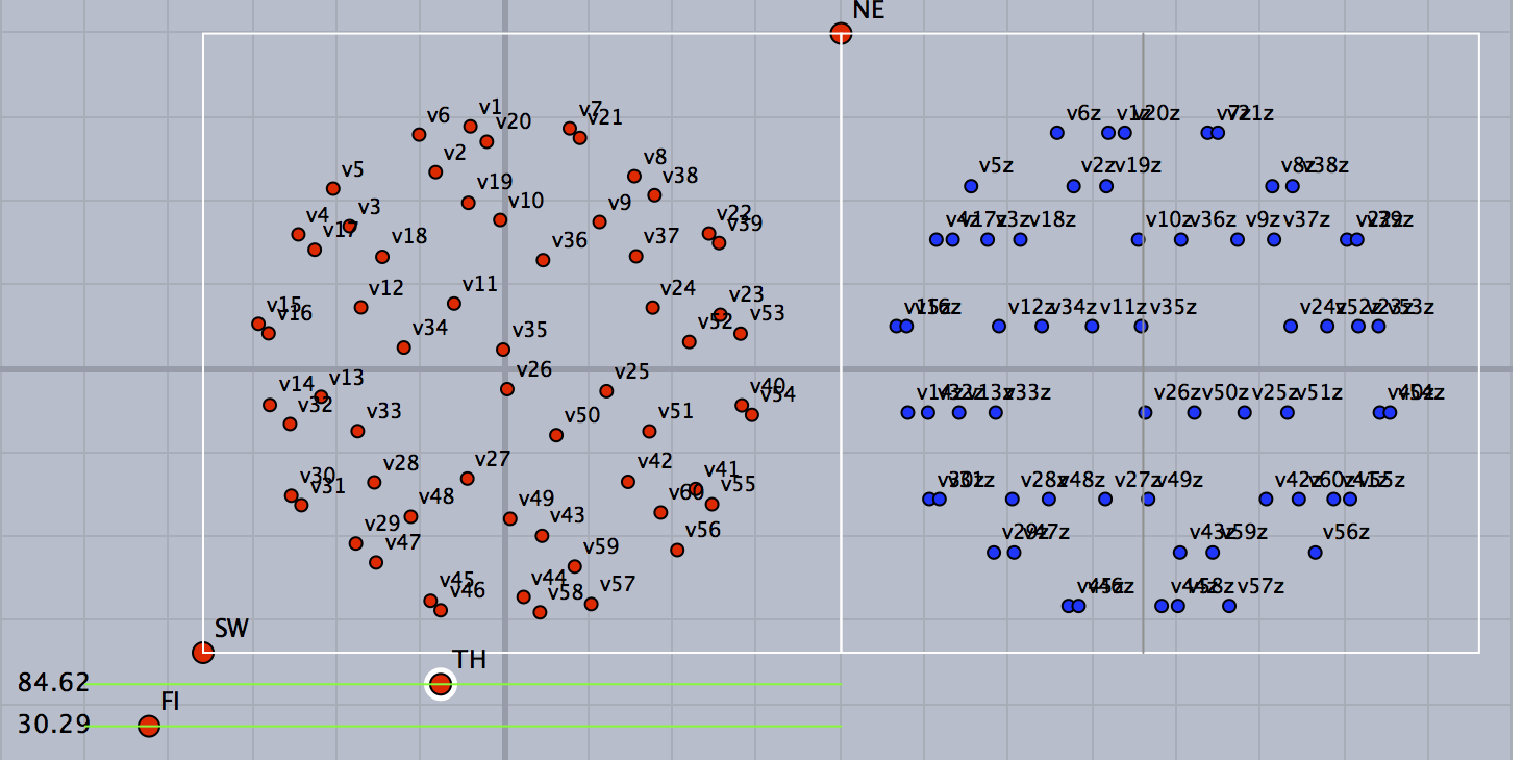
\includegraphics[bb=0 0 726.04 365.02 , width=10cm]{Fig/phparadata01.pdf}
\end{center}
 
\vspace{\baselineskip}
全体の線種と,陰線の線種を
  
\verb|Phparadata("1","s06",["dr,2","Hidden=do"]);|

で指定したのが下図右である。

 \begin{center} %%% /Users/Hannya/ketcindy/ketwork/template.tex 2016-8-11 22:26
%%% template.sce 2016-8-11 22:26
{\unitlength=6mm%
\begin{picture}%
(   7.60000,   7.37000)(  -3.60000,  -3.37000)%
\special{pn 8}%
%
\special{pa -98 -684}\special{pa -242 -660}%
\special{fp}%
\special{pa -242 -660}\special{pa -52 -640}%
\special{fp}%
\special{pa -52 -640}\special{pa 210 -651}%
\special{fp}%
\special{pa 210 -651}\special{pa 182 -678}%
\special{fp}%
\special{pa 182 -678}\special{pa -98 -684}%
\special{fp}%
\special{pa 182 -678}\special{pa 363 -543}%
\special{fp}%
\special{pa -582 -380}\special{pa -484 -508}%
\special{fp}%
\special{pa -484 -508}\special{pa -242 -660}%
\special{fp}%
\special{pa -662 100}\special{pa -694 -128}%
\special{fp}%
\special{pa -694 -128}\special{pa -582 -380}%
\special{fp}%
\special{pa -694 -128}\special{pa -666 -101}%
\special{fp}%
\special{pa -666 -101}\special{pa -536 -336}%
\special{fp}%
\special{pa -536 -336}\special{pa -484 -508}%
\special{fp}%
\special{pa -536 -336}\special{pa -346 -316}%
\special{fp}%
\special{pa -346 -316}\special{pa -104 -468}%
\special{fp}%
\special{pa -104 -468}\special{pa -52 -640}%
\special{fp}%
\special{pa 210 -651}\special{pa 420 -490}%
\special{fp}%
\special{pa 420 -490}\special{pa 602 -355}%
\special{fp}%
\special{pa 602 -355}\special{pa 573 -382}%
\special{fp}%
\special{pa 573 -382}\special{pa 363 -543}%
\special{fp}%
\special{pa -602 355}\special{pa -662 100}%
\special{fp}%
\special{pa -602 355}\special{pa -573 382}%
\special{fp}%
\special{pa -573 382}\special{pa -605 154}%
\special{fp}%
\special{pa -605 154}\special{pa -666 -101}%
\special{fp}%
\special{pa -605 154}\special{pa -415 174}%
\special{fp}%
\special{pa -415 174}\special{pa -285 -61}%
\special{fp}%
\special{pa -285 -61}\special{pa -346 -316}%
\special{fp}%
\special{pa -285 -61}\special{pa -6 -56}%
\special{fp}%
\special{pa -6 -56}\special{pa 106 -307}%
\special{fp}%
\special{pa 106 -307}\special{pa -104 -468}%
\special{fp}%
\special{pa 106 -307}\special{pa 368 -318}%
\special{fp}%
\special{pa 368 -318}\special{pa 420 -490}%
\special{fp}%
\special{pa 602 -355}\special{pa 662 -100}%
\special{fp}%
\special{pa 662 -100}\special{pa 694 128}%
\special{fp}%
\special{pa -182 678}\special{pa -363 543}%
\special{fp}%
\special{pa -363 543}\special{pa -573 382}%
\special{fp}%
\special{pa -363 543}\special{pa -265 415}%
\special{fp}%
\special{pa -265 415}\special{pa -415 174}%
\special{fp}%
\special{pa -265 415}\special{pa 14 420}%
\special{fp}%
\special{pa 14 420}\special{pa 144 185}%
\special{fp}%
\special{pa 144 185}\special{pa -6 -56}%
\special{fp}%
\special{pa 144 185}\special{pa 406 174}%
\special{fp}%
\special{pa 406 174}\special{pa 518 -77}%
\special{fp}%
\special{pa 518 -77}\special{pa 368 -318}%
\special{fp}%
\special{pa 518 -77}\special{pa 662 -100}%
\special{fp}%
\special{pa 694 128}\special{pa 582 380}%
\special{fp}%
\special{pa 582 380}\special{pa 484 508}%
\special{fp}%
\special{pa 484 508}\special{pa 242 660}%
\special{fp}%
\special{pa 242 660}\special{pa 98 684}%
\special{fp}%
\special{pa 98 684}\special{pa -182 678}%
\special{fp}%
\special{pa 98 684}\special{pa 196 555}%
\special{fp}%
\special{pa 196 555}\special{pa 14 420}%
\special{fp}%
\special{pa 196 555}\special{pa 438 403}%
\special{fp}%
\special{pa 438 403}\special{pa 406 174}%
\special{fp}%
\special{pa 438 403}\special{pa 582 380}%
\special{fp}%
\end{picture}}%   %%% /Users/Hannya/ketcindy/ketwork/template.tex 2016-8-11 22:33
%%% template.sce 2016-8-11 22:33
{\unitlength=6mm%
\begin{picture}%
(   7.60000,   7.37000)(  -3.60000,  -3.37000)%
\special{pn 8}%
%
\special{pn 16}%
\special{pa -98 -684}\special{pa -242 -660}%
\special{fp}%
\special{pa -242 -660}\special{pa -52 -640}%
\special{fp}%
\special{pa -52 -640}\special{pa 210 -651}%
\special{fp}%
\special{pa 210 -651}\special{pa 182 -678}%
\special{fp}%
\special{pa 182 -678}\special{pa -98 -684}%
\special{fp}%
\special{pa 182 -678}\special{pa 363 -543}%
\special{fp}%
\special{pa -582 -380}\special{pa -484 -508}%
\special{fp}%
\special{pa -484 -508}\special{pa -242 -660}%
\special{fp}%
\special{pa -662 100}\special{pa -694 -128}%
\special{fp}%
\special{pa -694 -128}\special{pa -582 -380}%
\special{fp}%
\special{pa -694 -128}\special{pa -666 -101}%
\special{fp}%
\special{pa -666 -101}\special{pa -536 -336}%
\special{fp}%
\special{pa -536 -336}\special{pa -484 -508}%
\special{fp}%
\special{pa -536 -336}\special{pa -346 -316}%
\special{fp}%
\special{pa -346 -316}\special{pa -104 -468}%
\special{fp}%
\special{pa -104 -468}\special{pa -52 -640}%
\special{fp}%
\special{pa 210 -651}\special{pa 420 -490}%
\special{fp}%
\special{pa 420 -490}\special{pa 602 -355}%
\special{fp}%
\special{pa 602 -355}\special{pa 573 -382}%
\special{fp}%
\special{pa 573 -382}\special{pa 363 -543}%
\special{fp}%
\special{pa -602 355}\special{pa -662 100}%
\special{fp}%
\special{pa -602 355}\special{pa -573 382}%
\special{fp}%
\special{pa -573 382}\special{pa -605 154}%
\special{fp}%
\special{pa -605 154}\special{pa -666 -101}%
\special{fp}%
\special{pa -605 154}\special{pa -415 174}%
\special{fp}%
\special{pa -415 174}\special{pa -285 -61}%
\special{fp}%
\special{pa -285 -61}\special{pa -346 -316}%
\special{fp}%
\special{pa -285 -61}\special{pa -6 -56}%
\special{fp}%
\special{pa -6 -56}\special{pa 106 -307}%
\special{fp}%
\special{pa 106 -307}\special{pa -104 -468}%
\special{fp}%
\special{pa 106 -307}\special{pa 368 -318}%
\special{fp}%
\special{pa 368 -318}\special{pa 420 -490}%
\special{fp}%
\special{pa 602 -355}\special{pa 662 -100}%
\special{fp}%
\special{pa 662 -100}\special{pa 694 128}%
\special{fp}%
\special{pa -182 678}\special{pa -363 543}%
\special{fp}%
\special{pa -363 543}\special{pa -573 382}%
\special{fp}%
\special{pa -363 543}\special{pa -265 415}%
\special{fp}%
\special{pa -265 415}\special{pa -415 174}%
\special{fp}%
\special{pa -265 415}\special{pa 14 420}%
\special{fp}%
\special{pa 14 420}\special{pa 144 185}%
\special{fp}%
\special{pa 144 185}\special{pa -6 -56}%
\special{fp}%
\special{pa 144 185}\special{pa 406 174}%
\special{fp}%
\special{pa 406 174}\special{pa 518 -77}%
\special{fp}%
\special{pa 518 -77}\special{pa 368 -318}%
\special{fp}%
\special{pa 518 -77}\special{pa 662 -100}%
\special{fp}%
\special{pa 694 128}\special{pa 582 380}%
\special{fp}%
\special{pa 582 380}\special{pa 484 508}%
\special{fp}%
\special{pa 484 508}\special{pa 242 660}%
\special{fp}%
\special{pa 242 660}\special{pa 98 684}%
\special{fp}%
\special{pa 98 684}\special{pa -182 678}%
\special{fp}%
\special{pa 98 684}\special{pa 196 555}%
\special{fp}%
\special{pa 196 555}\special{pa 14 420}%
\special{fp}%
\special{pa 196 555}\special{pa 438 403}%
\special{fp}%
\special{pa 438 403}\special{pa 406 174}%
\special{fp}%
\special{pa 438 403}\special{pa 582 380}%
\special{fp}%
\special{pn 8}%
\special{pn 8}%
\special{pa -95 -687}\special{pa -100 -680}\special{fp}\special{pa -120 -655}\special{pa -125 -648}\special{fp}%
\special{pa -144 -622}\special{pa -149 -616}\special{fp}\special{pa -169 -590}\special{pa -174 -584}\special{fp}%
\special{pa -193 -558}\special{pa -198 -552}\special{fp}\special{pn 8}%
\special{pa -192 -557}\special{pa -199 -553}\special{fp}\special{pa -227 -535}\special{pa -234 -531}\special{fp}%
\special{pa -261 -513}\special{pa -268 -509}\special{fp}\special{pa -296 -492}\special{pa -303 -488}\special{fp}%
\special{pa -331 -470}\special{pa -337 -466}\special{fp}\special{pa -365 -448}\special{pa -372 -444}\special{fp}%
\special{pa -400 -427}\special{pa -407 -422}\special{fp}\special{pa -434 -405}\special{pa -441 -401}\special{fp}%
\special{pn 8}%
\special{pa -586 -379}\special{pa -578 -380}\special{fp}\special{pa -550 -385}\special{pa -542 -386}\special{fp}%
\special{pa -514 -391}\special{pa -506 -392}\special{fp}\special{pa -478 -396}\special{pa -470 -398}\special{fp}%
\special{pa -442 -402}\special{pa -434 -403}\special{fp}\special{pn 8}%
\special{pa -438 -407}\special{pa -437 -399}\special{fp}\special{pa -433 -369}\special{pa -432 -361}\special{fp}%
\special{pa -428 -331}\special{pa -426 -323}\special{fp}\special{pa -422 -293}\special{pa -421 -285}\special{fp}%
\special{pa -417 -254}\special{pa -416 -247}\special{fp}\special{pa -412 -216}\special{pa -410 -209}\special{fp}%
\special{pa -406 -178}\special{pa -405 -170}\special{fp}\special{pn 8}%
\special{pa -404 -178}\special{pa -407 -171}\special{fp}\special{pa -420 -142}\special{pa -423 -135}\special{fp}%
\special{pa -436 -106}\special{pa -439 -99}\special{fp}\special{pa -452 -70}\special{pa -455 -63}\special{fp}%
\special{pa -468 -34}\special{pa -471 -27}\special{fp}\special{pa -484 2}\special{pa -487 9}\special{fp}%
\special{pa -500 38}\special{pa -504 45}\special{fp}\special{pa -516 74}\special{pa -520 81}\special{fp}%
\special{pn 8}%
\special{pa -666 101}\special{pa -658 100}\special{fp}\special{pa -630 95}\special{pa -622 94}\special{fp}%
\special{pa -594 89}\special{pa -586 88}\special{fp}\special{pa -558 84}\special{pa -550 82}\special{fp}%
\special{pa -522 78}\special{pa -514 77}\special{fp}\special{pn 8}%
\special{pa -410 -174}\special{pa -402 -175}\special{fp}\special{pa -372 -176}\special{pa -364 -176}\special{fp}%
\special{pa -335 -177}\special{pa -327 -178}\special{fp}\special{pa -297 -179}\special{pa -289 -179}\special{fp}%
\special{pa -260 -180}\special{pa -252 -181}\special{fp}\special{pa -223 -182}\special{pa -215 -182}\special{fp}%
\special{pa -185 -183}\special{pa -177 -184}\special{fp}\special{pa -148 -185}\special{pa -140 -185}\special{fp}%
\special{pn 8}%
\special{pa 366 -547}\special{pa 361 -540}\special{fp}\special{pa 341 -514}\special{pa 336 -508}\special{fp}%
\special{pa 317 -482}\special{pa 312 -476}\special{fp}\special{pa 292 -450}\special{pa 287 -444}\special{fp}%
\special{pa 268 -418}\special{pa 263 -411}\special{fp}\special{pn 8}%
\special{pa 269 -414}\special{pa 261 -415}\special{fp}\special{pa 229 -415}\special{pa 221 -415}\special{fp}%
\special{pa 190 -416}\special{pa 182 -416}\special{fp}\special{pa 150 -417}\special{pa 142 -417}\special{fp}%
\special{pa 110 -418}\special{pa 102 -418}\special{fp}\special{pa 70 -419}\special{pa 62 -419}\special{fp}%
\special{pa 30 -419}\special{pa 22 -420}\special{fp}\special{pa -10 -420}\special{pa -18 -420}\special{fp}%
\special{pn 8}%
\special{pa -199 -557}\special{pa -192 -552}\special{fp}\special{pa -169 -535}\special{pa -162 -530}\special{fp}%
\special{pa -138 -512}\special{pa -132 -508}\special{fp}\special{pa -108 -490}\special{pa -102 -485}\special{fp}%
\special{pa -78 -467}\special{pa -71 -463}\special{fp}\special{pa -48 -445}\special{pa -41 -440}\special{fp}%
\special{pa -17 -423}\special{pa -11 -418}\special{fp}\special{pn 8}%
\special{pa -146 -182}\special{pa -142 -189}\special{fp}\special{pa -127 -215}\special{pa -123 -222}\special{fp}%
\special{pa -109 -249}\special{pa -105 -256}\special{fp}\special{pa -90 -282}\special{pa -86 -289}\special{fp}%
\special{pa -72 -316}\special{pa -68 -323}\special{fp}\special{pa -53 -350}\special{pa -49 -357}\special{fp}%
\special{pa -35 -383}\special{pa -31 -390}\special{fp}\special{pa -16 -417}\special{pa -12 -424}\special{fp}%
\special{pn 8}%
\special{pa -520 74}\special{pa -516 81}\special{fp}\special{pa -499 108}\special{pa -494 115}\special{fp}%
\special{pa -477 143}\special{pa -473 149}\special{fp}\special{pa -456 177}\special{pa -452 184}\special{fp}%
\special{pa -435 211}\special{pa -430 218}\special{fp}\special{pa -413 246}\special{pa -409 253}\special{fp}%
\special{pa -392 280}\special{pa -388 287}\special{fp}\special{pa -370 315}\special{pa -366 321}\special{fp}%
\special{pn 8}%
\special{pa -367 314}\special{pa -369 322}\special{fp}\special{pa -378 349}\special{pa -380 356}\special{fp}%
\special{pa -388 383}\special{pa -390 391}\special{fp}\special{pa -398 417}\special{pa -401 425}\special{fp}%
\special{pa -409 452}\special{pa -411 459}\special{fp}\special{pa -419 486}\special{pa -421 494}\special{fp}%
\special{pn 8}%
\special{pa -605 353}\special{pa -599 358}\special{fp}\special{pa -575 375}\special{pa -568 380}\special{fp}%
\special{pa -544 398}\special{pa -538 403}\special{fp}\special{pa -514 420}\special{pa -508 425}\special{fp}%
\special{pa -484 443}\special{pa -477 447}\special{fp}\special{pa -454 465}\special{pa -447 470}\special{fp}%
\special{pa -423 488}\special{pa -417 492}\special{fp}\special{pn 8}%
\special{pa -146 -189}\special{pa -142 -182}\special{fp}\special{pa -125 -154}\special{pa -120 -147}\special{fp}%
\special{pa -103 -120}\special{pa -99 -113}\special{fp}\special{pa -82 -85}\special{pa -78 -79}\special{fp}%
\special{pa -60 -51}\special{pa -56 -44}\special{fp}\special{pa -39 -17}\special{pa -35 -10}\special{fp}%
\special{pa -18 18}\special{pa -13 25}\special{fp}\special{pa 4 52}\special{pa 8 59}\special{fp}%
\special{pn 8}%
\special{pa 7 52}\special{pa 4 59}\special{fp}\special{pa -9 88}\special{pa -12 95}\special{fp}%
\special{pa -25 124}\special{pa -28 131}\special{fp}\special{pa -41 160}\special{pa -44 167}\special{fp}%
\special{pa -57 196}\special{pa -60 203}\special{fp}\special{pa -73 232}\special{pa -76 239}\special{fp}%
\special{pa -89 268}\special{pa -92 275}\special{fp}\special{pa -105 304}\special{pa -108 311}\special{fp}%
\special{pn 8}%
\special{pa -372 318}\special{pa -364 318}\special{fp}\special{pa -335 317}\special{pa -327 316}\special{fp}%
\special{pa -298 315}\special{pa -290 315}\special{fp}\special{pa -260 314}\special{pa -252 313}\special{fp}%
\special{pa -223 312}\special{pa -215 312}\special{fp}\special{pa -185 310}\special{pa -177 310}\special{fp}%
\special{pa -148 309}\special{pa -140 309}\special{fp}\special{pa -110 307}\special{pa -102 307}\special{fp}%
\special{pn 8}%
\special{pa 263 -418}\special{pa 268 -411}\special{fp}\special{pa 285 -384}\special{pa 289 -377}\special{fp}%
\special{pa 306 -349}\special{pa 310 -342}\special{fp}\special{pa 327 -315}\special{pa 332 -308}\special{fp}%
\special{pa 349 -280}\special{pa 353 -274}\special{fp}\special{pa 370 -246}\special{pa 374 -239}\special{fp}%
\special{pa 392 -212}\special{pa 396 -205}\special{fp}\special{pa 413 -177}\special{pa 417 -170}\special{fp}%
\special{pn 8}%
\special{pa 417 -177}\special{pa 413 -170}\special{fp}\special{pa 398 -144}\special{pa 395 -137}\special{fp}%
\special{pa 380 -110}\special{pa 376 -103}\special{fp}\special{pa 361 -77}\special{pa 357 -70}\special{fp}%
\special{pa 343 -43}\special{pa 339 -36}\special{fp}\special{pa 324 -9}\special{pa 320 -2}\special{fp}%
\special{pa 306 24}\special{pa 302 31}\special{fp}\special{pa 287 58}\special{pa 283 65}\special{fp}%
\special{pn 8}%
\special{pa 2 56}\special{pa 10 56}\special{fp}\special{pa 42 56}\special{pa 50 57}\special{fp}%
\special{pa 82 57}\special{pa 90 57}\special{fp}\special{pa 122 58}\special{pa 130 58}\special{fp}%
\special{pa 161 59}\special{pa 169 59}\special{fp}\special{pa 201 60}\special{pa 209 60}\special{fp}%
\special{pa 241 60}\special{pa 249 61}\special{fp}\special{pa 281 61}\special{pa 289 61}\special{fp}%
\special{pn 8}%
\special{pa 573 -386}\special{pa 574 -378}\special{fp}\special{pa 578 -348}\special{pa 579 -340}\special{fp}%
\special{pa 583 -310}\special{pa 585 -302}\special{fp}\special{pa 589 -272}\special{pa 590 -264}\special{fp}%
\special{pa 594 -234}\special{pa 595 -226}\special{fp}\special{pa 599 -196}\special{pa 601 -188}\special{fp}%
\special{pa 605 -158}\special{pa 606 -150}\special{fp}\special{pn 8}%
\special{pa 411 -174}\special{pa 419 -173}\special{fp}\special{pa 449 -170}\special{pa 457 -169}\special{fp}%
\special{pa 487 -166}\special{pa 495 -165}\special{fp}\special{pa 525 -162}\special{pa 533 -161}\special{fp}%
\special{pa 563 -158}\special{pa 571 -157}\special{fp}\special{pa 601 -154}\special{pa 609 -153}\special{fp}%
\special{pn 8}%
\special{pa 56 640}\special{pa 48 641}\special{fp}\special{pa 18 642}\special{pa 10 642}\special{fp}%
\special{pa -19 643}\special{pa -27 644}\special{fp}\special{pa -56 645}\special{pa -64 645}\special{fp}%
\special{pa -94 646}\special{pa -102 647}\special{fp}\special{pa -131 648}\special{pa -139 648}\special{fp}%
\special{pa -169 649}\special{pa -177 650}\special{fp}\special{pa -206 651}\special{pa -214 651}\special{fp}%
\special{pn 8}%
\special{pa -423 488}\special{pa -417 492}\special{fp}\special{pa -393 511}\special{pa -387 515}\special{fp}%
\special{pa -363 534}\special{pa -357 538}\special{fp}\special{pa -333 557}\special{pa -327 561}\special{fp}%
\special{pa -303 580}\special{pa -297 584}\special{fp}\special{pa -273 603}\special{pa -267 608}\special{fp}%
\special{pa -243 626}\special{pa -237 631}\special{fp}\special{pa -213 649}\special{pa -207 654}\special{fp}%
\special{pn 8}%
\special{pa -213 648}\special{pa -207 654}\special{fp}\special{pa -185 675}\special{pa -179 681}\special{fp}%
\special{pn 8}%
\special{pa 284 57}\special{pa 286 65}\special{fp}\special{pa 293 94}\special{pa 295 102}\special{fp}%
\special{pa 302 130}\special{pa 303 138}\special{fp}\special{pa 310 167}\special{pa 312 175}\special{fp}%
\special{pa 319 203}\special{pa 321 211}\special{fp}\special{pa 327 240}\special{pa 329 247}\special{fp}%
\special{pa 336 276}\special{pa 338 284}\special{fp}\special{pa 345 313}\special{pa 347 320}\special{fp}%
\special{pn 8}%
\special{pa 349 314}\special{pa 342 319}\special{fp}\special{pa 314 336}\special{pa 308 340}\special{fp}%
\special{pa 280 358}\special{pa 273 362}\special{fp}\special{pa 245 379}\special{pa 239 384}\special{fp}%
\special{pa 211 401}\special{pa 204 405}\special{fp}\special{pa 176 423}\special{pa 169 427}\special{fp}%
\special{pa 142 445}\special{pa 135 449}\special{fp}\special{pa 107 466}\special{pa 100 471}\special{fp}%
\special{pn 8}%
\special{pa -110 305}\special{pa -103 310}\special{fp}\special{pa -80 328}\special{pa -73 333}\special{fp}%
\special{pa -50 351}\special{pa -43 356}\special{fp}\special{pa -20 374}\special{pa -13 379}\special{fp}%
\special{pa 10 397}\special{pa 17 402}\special{fp}\special{pa 40 420}\special{pa 47 425}\special{fp}%
\special{pa 70 443}\special{pa 77 448}\special{fp}\special{pa 100 466}\special{pa 107 471}\special{fp}%
\special{pn 8}%
\special{pa 51 644}\special{pa 53 637}\special{fp}\special{pa 61 610}\special{pa 63 602}\special{fp}%
\special{pa 71 575}\special{pa 74 568}\special{fp}\special{pa 82 541}\special{pa 84 533}\special{fp}%
\special{pa 92 507}\special{pa 94 499}\special{fp}\special{pa 102 472}\special{pa 105 465}\special{fp}%
\special{pn 8}%
\special{pa 697 131}\special{pa 691 125}\special{fp}\special{pa 669 104}\special{pa 663 99}\special{fp}%
\special{pn 8}%
\special{pa 604 -158}\special{pa 606 -150}\special{fp}\special{pa 613 -121}\special{pa 615 -113}\special{fp}%
\special{pa 622 -85}\special{pa 623 -77}\special{fp}\special{pa 630 -48}\special{pa 632 -41}\special{fp}%
\special{pa 639 -12}\special{pa 641 -4}\special{fp}\special{pa 648 25}\special{pa 649 32}\special{fp}%
\special{pa 656 61}\special{pa 658 69}\special{fp}\special{pa 665 97}\special{pa 667 105}\special{fp}%
\special{pn 8}%
\special{pa 668 98}\special{pa 664 105}\special{fp}\special{pa 649 131}\special{pa 645 138}\special{fp}%
\special{pa 631 165}\special{pa 627 172}\special{fp}\special{pa 612 199}\special{pa 608 206}\special{fp}%
\special{pa 593 232}\special{pa 590 239}\special{fp}\special{pa 575 266}\special{pa 571 273}\special{fp}%
\special{pa 556 299}\special{pa 553 306}\special{fp}\special{pa 538 333}\special{pa 534 340}\special{fp}%
\special{pn 8}%
\special{pa 342 316}\special{pa 350 317}\special{fp}\special{pa 380 320}\special{pa 388 321}\special{fp}%
\special{pa 418 324}\special{pa 426 325}\special{fp}\special{pa 456 328}\special{pa 464 329}\special{fp}%
\special{pa 494 332}\special{pa 502 333}\special{fp}\special{pa 532 336}\special{pa 540 337}\special{fp}%
\special{pn 8}%
\special{pa 537 333}\special{pa 535 340}\special{fp}\special{pa 527 367}\special{pa 524 375}\special{fp}%
\special{pa 516 401}\special{pa 514 409}\special{fp}\special{pa 506 436}\special{pa 504 443}\special{fp}%
\special{pa 496 470}\special{pa 493 478}\special{fp}\special{pa 485 505}\special{pa 483 512}\special{fp}%
\special{pn 8}%
\special{pa 48 640}\special{pa 56 641}\special{fp}\special{pa 86 644}\special{pa 94 645}\special{fp}%
\special{pa 124 648}\special{pa 132 649}\special{fp}\special{pa 162 652}\special{pa 170 653}\special{fp}%
\special{pa 200 656}\special{pa 208 657}\special{fp}\special{pa 238 660}\special{pa 246 661}\special{fp}%
\special{pn 8}%
\end{picture}}% \end{center}

【注意】

  polyhedrons obj のデータを使って,続けて異なる多面体を描きたい場合は注意が必要である。Readobj()だけを変更して別のデータを読めばよさそうであるが,VertexEdgeFace() のname も(したがって,Phparadata()の第2引数も)書き換えないと,前のデータが残っていてうまくいかない。たとえば,上のコードで切頂二十面体を描いた後,正八面体(r02)を描こうとするならば,
\begin{verbatim}
  Setdirectory( Dirhead+"/data/polyhedrons_obj");
  phd=Readobj("r02.obj",["size=3"]);
  Setdirectory(Dirwork);
  VertexEdgeFace("2",phd,["Edg=nogeo"]);
  Phparadata("1","2");
\end{verbatim}
  のようにする。
  

\begin{flushright} \hyperlink{functionlist}{$\Rightarrow$関数一覧}\end{flushright}

\hypertarget{pointdata3d}{}
\item[関数]  Pointdata3d(名前,点リスト,options)
\item[機能]  点の3Dデータと2Dデータを作成し,画面と\TeX に出力する。
\item[説明]  optionsは\hyperlink{pointdata}{Pointdata()}と同様。
\vspace{\baselineskip}

【例】
\begin{verbatim}
  Pointdata3d("1",[[1,1,1],[0,1,0]],["Size=2","Color=red"]);
\end{verbatim}
\vspace{\baselineskip}

\begin{flushright} \hyperlink{functionlist}{$\Rightarrow$関数一覧}\end{flushright}

\hypertarget{projcoordpara}{}
\item[関数]  Projcoordpara(座標)
\item[機能]  投影座標を求める
\item[説明]  空間座標を平面に投影した座標を求める。

戻り値の第1,第2要素はCinderellaの描画面のx,y座標。第3要素はxy平面に垂直なzの座標で.投影面からの(符号付)距離を表す。

\vspace{\baselineskip}
【例】\verb|Projcoordpara([3,1,2]);|

 戻り値は  [-0.65,1.7,3.27]   のようになる。(視点によって値は異なる)


\vspace{\baselineskip}
\hypertarget{putaxes3d}{}
\item[関数]  Putaxes3d([x,y,z])
\item[機能]  軸上に幾何点を作る。
\item[説明]  引数のリスト [x,y,z] に対し,点X(x,0,0) ,Y(0,y,0) , Z(0,0,z) および 原点Oを主画面上にとり,副画面上に対応する点Xz,Yz,Zz,Oz を作る。すでに同じ名称の点がある場合は,指定された位置に移動する。

引数は,実数にすることもでき,Putaxes3d(a) は,Putaxes3d([a,a,a]) と同じになる。
  
\vspace{\baselineskip}
【例】Putaxes3d(5);  原点と,$x(5,0,0),y(0,5,0),z(0,0,5)$ を作る。

 Putaxes3d([1,2,3]);  原点と,$x(1,0,0),y(0,2,0),z(0,0,3)$ を作る。

\begin{flushright} \hyperlink{functionlist}{$\Rightarrow$関数一覧}\end{flushright}

\vspace{\baselineskip}
\hypertarget{putonCurve3d}{}
\item[関数]  PutonCurve3d(点名,PD)
\item[機能]  空間曲線上に点をとる
\item[説明]  プロットデータPDの曲線上に,点名の点をとる。

とった点は固定点ではなく,曲線上にインシデントとなる。したがって,ドラッグして曲線上を動かすことができる。例は \hyperlink{partcrv3d}{Partcrv3d()} を参照のこと。

\vspace{\baselineskip}
\hypertarget{putonseg3d}{}
\item[関数]  Putonseg3d(点名,点1,点2)
\item[機能]  線分上に点を作る
\item[説明]  点1と点2の中点に,指定された名前の点を取る。点1と点2が線分として結ばれていなくてもよい。とった点は線分にインシデントとなる(線分が描かれていなくても)。点1と点2はリストにすることもできる。指定した点がすでに存在する場合は動かさない。

点1,点2は幾何点の名称または座標で指定する。

\vspace{\baselineskip}
【例】A(1,-1,0)とB(0,2,2) の中点に点Cをとる。つぎのいずれでもよい。

    \verb|Putonseg3d("C",A,B);|

    \verb|Putonseg3d("C",[A,B]);|
    
    \verb|Putonseg3d("C",[[1,-1,0],[0,2,2]]);|

\vspace{\baselineskip}

\hypertarget{putpoint3d}{}
\item[関数]  Putpoint3d(リスト,option)
\item[機能]  空間に幾何点を作図する
\item[説明]  点の名称と座標を与えて点を作図する。複数の点を一度に作図できる。

optionは,"fix" または "free" ( 初期設定)。
 
"fix" をつけると,固定点(ドラッグで移動できない点)とする。同じ名称の点がすでに存在する場合は,指定した位置に移動して固定点とする。

"free" をつけると,自由点(ドラッグで移動できる)とする。同じ名称の点がすでに存在する場合はなにもしない。

\vspace{\baselineskip}
【例】いくつか記述例を示す。

    \verb|Putpoint3d(["A",[2,1,3]]);|
    
    \verb|Putpoint3d(["A",[1,1,1],"C",[1,0,1]],"fix");|
    
    \verb|Putpoint3d(["A",[2,1,3]],"free");|
    
\vspace{\baselineskip}
  なお,この関数は幾何点を作るものであり,TeXには出力されない。TeXに点を出力するには,\hyperlink{pointdata}{Pointdata()} または \hyperlink{drwpt}{Drawpoint()}を併用する。
  
  空間における点の座標は,点名に"3d"を付加した名前の変数に代入される。たとえば,点Aの座標はA3dである。これにより,点の座標を取得できる。

\begin{flushright} \hyperlink{functionlist}{$\Rightarrow$関数一覧}\end{flushright}

\vspace{\baselineskip}
\hypertarget{readobj}{}
\item[関数]  Readobj(ファイル名)
\item[機能]  objファイルを読み込む。
\item[説明]  小林・鈴木・三谷による整面凸多面体のデータは\\
\hspace*{20mm}\url{http://mitani.cs.tsukuba.ac.jp/polyhedron/}\\
からダウンロードできる。\verb|polyhedrons_obj|を,例えば,ユーザホームのketcindy作業フォルダに入れておく。
\begin{verbatim}
  Setdirectory(gethome()+"/ketcindy/polyhedrons_obj");
  polydt=Readobj("r02.obj");
  Setdirectory(Dirwork);
\end{verbatim}
これで,r02.obj データが,変数 polydt に代入される。

オプションは "size=n"  で,n倍したデータにする。負の数にすると上下が反転される。

データはKeTCindyのdataフォルダの中にある。したがって,次のようなスクリプトを書く。読み込むのは一度だけなので, Draw スロットではなくInitialization スロットに置けばよいが,コードの可読性を高めるには Draw スロットでもよい。

この多面体データは,頂点リストと面リストからなっているが,頂点リストは座標のリストなので,読み込んで表示するときには,点の名称を v1,v2,・・・ とする。

読み込んだあとの使い方を含めて例を示す。

\begin{layer}{150}{0}
\putnotese{80}{0}{ %%% /Users/Hannya/ketcindy/ketwork/template.tex 2016-8-9 20:2
%%% template.sce 2016-8-9 20:2
{\unitlength=8mm%
\begin{picture}%
(   6.00000,   5.00000)(  -3.00000,  -2.00000)%
\special{pn 8}%
%
\special{pn 8}%
\special{pa -59 -253}\special{pa -51 -251}\special{fp}\special{pa -21 -240}\special{pa -13 -238}\special{fp}%
\special{pa 17 -228}\special{pa 25 -225}\special{fp}\special{pa 55 -215}\special{pa 62 -212}\special{fp}%
\special{pa 93 -202}\special{pa 100 -200}\special{fp}\special{pa 130 -189}\special{pa 138 -187}\special{fp}%
\special{pa 168 -177}\special{pa 176 -174}\special{fp}\special{pa 206 -164}\special{pa 214 -161}\special{fp}%
\special{pa 244 -151}\special{pa 251 -148}\special{fp}\special{pa 282 -138}\special{pa 289 -136}\special{fp}%
\special{pa 319 -125}\special{pa 327 -123}\special{fp}\special{pa 357 -113}\special{pa 365 -110}\special{fp}%
\special{pa 395 -100}\special{pa 403 -97}\special{fp}\special{pa 433 -87}\special{pa 440 -85}\special{fp}%
\special{pa 471 -74}\special{pa 478 -72}\special{fp}\special{pa 508 -62}\special{pa 516 -59}\special{fp}%
\special{pa 546 -49}\special{pa 554 -46}\special{fp}\special{pa 584 -36}\special{pa 592 -34}\special{fp}%
\special{pa 622 -23}\special{pa 629 -21}\special{fp}\special{pn 8}%
\special{pa 626 -22}\special{pa 0 577}%
\special{fp}%
\special{pn 8}%
\special{pa -55 -256}\special{pa -54 -248}\special{fp}\special{pa -52 -216}\special{pa -52 -208}\special{fp}%
\special{pa -50 -177}\special{pa -49 -169}\special{fp}\special{pa -47 -138}\special{pa -47 -130}\special{fp}%
\special{pa -45 -98}\special{pa -44 -90}\special{fp}\special{pa -42 -59}\special{pa -41 -51}\special{fp}%
\special{pa -39 -19}\special{pa -39 -11}\special{fp}\special{pa -37 20}\special{pa -36 28}\special{fp}%
\special{pa -34 60}\special{pa -34 68}\special{fp}\special{pa -32 99}\special{pa -31 107}\special{fp}%
\special{pa -29 139}\special{pa -28 147}\special{fp}\special{pa -26 178}\special{pa -26 186}\special{fp}%
\special{pa -24 218}\special{pa -23 226}\special{fp}\special{pa -21 257}\special{pa -21 265}\special{fp}%
\special{pa -19 296}\special{pa -18 304}\special{fp}\special{pa -16 336}\special{pa -15 344}\special{fp}%
\special{pa -13 375}\special{pa -13 383}\special{fp}\special{pa -11 415}\special{pa -10 423}\special{fp}%
\special{pa -8 454}\special{pa -8 462}\special{fp}\special{pa -5 494}\special{pa -5 502}\special{fp}%
\special{pa -3 533}\special{pa -2 541}\special{fp}\special{pa 0 573}\special{pa 0 581}\special{fp}%
\special{pn 8}%
\special{pa -626 22}\special{pa 0 577}%
\special{fp}%
\special{pn 8}%
\special{pa -51 -254}\special{pa -58 -250}\special{fp}\special{pa -87 -237}\special{pa -94 -233}\special{fp}%
\special{pa -122 -219}\special{pa -130 -216}\special{fp}\special{pa -158 -202}\special{pa -165 -199}\special{fp}%
\special{pa -194 -185}\special{pa -201 -182}\special{fp}\special{pa -230 -168}\special{pa -237 -165}\special{fp}%
\special{pa -265 -151}\special{pa -272 -147}\special{fp}\special{pa -301 -134}\special{pa -308 -130}\special{fp}%
\special{pa -337 -117}\special{pa -344 -113}\special{fp}\special{pa -372 -100}\special{pa -379 -96}\special{fp}%
\special{pa -408 -82}\special{pa -415 -79}\special{fp}\special{pa -444 -65}\special{pa -451 -62}\special{fp}%
\special{pa -479 -48}\special{pa -487 -45}\special{fp}\special{pa -515 -31}\special{pa -522 -28}\special{fp}%
\special{pa -551 -14}\special{pa -558 -10}\special{fp}\special{pa -586 3}\special{pa -594 7}\special{fp}%
\special{pa -622 20}\special{pa -629 24}\special{fp}\special{pn 8}%
\special{pa -626 22}\special{pa 0 -577}%
\special{fp}%
\special{pn 8}%
\special{pa -55 -248}\special{pa -54 -256}\special{fp}\special{pa -49 -289}\special{pa -47 -296}\special{fp}%
\special{pa -42 -329}\special{pa -40 -337}\special{fp}\special{pa -35 -370}\special{pa -34 -378}\special{fp}%
\special{pa -28 -410}\special{pa -27 -418}\special{fp}\special{pa -21 -451}\special{pa -20 -459}\special{fp}%
\special{pa -14 -491}\special{pa -13 -499}\special{fp}\special{pa -8 -532}\special{pa -6 -540}\special{fp}%
\special{pa -1 -573}\special{pa 1 -581}\special{fp}\special{pn 8}%
\special{pa 626 -22}\special{pa 0 -577}%
\special{fp}%
\special{pa 626 -22}\special{pa 55 252}%
\special{fp}%
\special{pa 55 252}\special{pa 0 577}%
\special{fp}%
\special{pa 55 252}\special{pa 0 -577}%
\special{fp}%
\special{pa 55 252}\special{pa -626 22}%
\special{fp}%
\end{picture}}%}
\end{layer}


\vspace{\baselineskip}
【例】\verb|polydt|を用いて正八面体を描く


\begin{verbatim}

  VertexEdgeFace("1",polydt,["Edg=nogeo"]);
  Nohiddenbyfaces("1","phf3d1");
\end{verbatim}

主なデータは次の通り。

\vspace{\baselineskip}
 %%% /Users/Hannya/Desktop/KeTCindy/KeTCindyTools/fig/table.tex 
%%% Generator=作表.cdy 
{\unitlength=10mm%
\begin{picture}%
(13,5.6)(0,0)%
\special{pn 8}%
%
\special{pa     0 -2205}\special{pa     0    -0}%
\special{fp}%
\special{pa   394 -2205}\special{pa   394    -0}%
\special{fp}%
\special{pa  1378 -2205}\special{pa  1378    -0}%
\special{fp}%
\special{pa  1772 -2205}\special{pa  1772    -0}%
\special{fp}%
\special{pa  2953 -2205}\special{pa  2953    -0}%
\special{fp}%
\special{pa  3543 -2205}\special{pa  3543    -0}%
\special{fp}%
\special{pa  5118 -2205}\special{pa  5118    -0}%
\special{fp}%
\special{pa     0 -2205}\special{pa  5118 -2205}%
\special{fp}%
\special{pa     0 -1890}\special{pa  5118 -1890}%
\special{fp}%
\special{pa     0 -1575}\special{pa  5118 -1575}%
\special{fp}%
\special{pa     0 -1260}\special{pa  5118 -1260}%
\special{fp}%
\special{pa     0  -945}\special{pa  5118  -945}%
\special{fp}%
\special{pa     0  -630}\special{pa  5118  -630}%
\special{fp}%
\special{pa     0  -315}\special{pa  5118  -315}%
\special{fp}%
\special{pa     0    -0}\special{pa  5118    -0}%
\special{fp}%
\settowidth{\Width}{番号}\setlength{\Width}{-0.5\Width}%
\settoheight{\Height}{番号}\settodepth{\Depth}{番号}\setlength{\Height}{-0.5\Height}\setlength{\Depth}{0.5\Depth}\addtolength{\Height}{\Depth}%
\put(0.5000000,5.2000000){\hspace*{\Width}\raisebox{\Height}{番号}}%
%
\settowidth{\Width}{名称}\setlength{\Width}{-0.5\Width}%
\settoheight{\Height}{名称}\settodepth{\Depth}{名称}\setlength{\Height}{-0.5\Height}\setlength{\Depth}{0.5\Depth}\addtolength{\Height}{\Depth}%
\put(2.2500000,5.2000000){\hspace*{\Width}\raisebox{\Height}{名称}}%
%
\settowidth{\Width}{番号}\setlength{\Width}{-0.5\Width}%
\settoheight{\Height}{番号}\settodepth{\Depth}{番号}\setlength{\Height}{-0.5\Height}\setlength{\Depth}{0.5\Depth}\addtolength{\Height}{\Depth}%
\put(4.0000000,5.2000000){\hspace*{\Width}\raisebox{\Height}{番号}}%
%
\settowidth{\Width}{名称}\setlength{\Width}{-0.5\Width}%
\settoheight{\Height}{名称}\settodepth{\Depth}{名称}\setlength{\Height}{-0.5\Height}\setlength{\Depth}{0.5\Depth}\addtolength{\Height}{\Depth}%
\put(6.0000000,5.2000000){\hspace*{\Width}\raisebox{\Height}{名称}}%
%
\settowidth{\Width}{番号}\setlength{\Width}{-0.5\Width}%
\settoheight{\Height}{番号}\settodepth{\Depth}{番号}\setlength{\Height}{-0.5\Height}\setlength{\Depth}{0.5\Depth}\addtolength{\Height}{\Depth}%
\put(8.2500000,5.2000000){\hspace*{\Width}\raisebox{\Height}{番号}}%
%
\settowidth{\Width}{名称}\setlength{\Width}{-0.5\Width}%
\settoheight{\Height}{名称}\settodepth{\Depth}{名称}\setlength{\Height}{-0.5\Height}\setlength{\Depth}{0.5\Depth}\addtolength{\Height}{\Depth}%
\put(11.0000000,5.2000000){\hspace*{\Width}\raisebox{\Height}{名称}}%
%
\settowidth{\Width}{r01}\setlength{\Width}{-0.5\Width}%
\settoheight{\Height}{r01}\settodepth{\Depth}{r01}\setlength{\Height}{-0.5\Height}\setlength{\Depth}{0.5\Depth}\addtolength{\Height}{\Depth}%
\put(0.5000000,4.4000000){\hspace*{\Width}\raisebox{\Height}{r01}}%
%
\settowidth{\Width}{正四面体}\setlength{\Width}{-0.5\Width}%
\settoheight{\Height}{正四面体}\settodepth{\Depth}{正四面体}\setlength{\Height}{-0.5\Height}\setlength{\Depth}{0.5\Depth}\addtolength{\Height}{\Depth}%
\put(2.2500000,4.4000000){\hspace*{\Width}\raisebox{\Height}{正四面体}}%
%
\settowidth{\Width}{s02}\setlength{\Width}{-0.5\Width}%
\settoheight{\Height}{s02}\settodepth{\Depth}{s02}\setlength{\Height}{-0.5\Height}\setlength{\Depth}{0.5\Depth}\addtolength{\Height}{\Depth}%
\put(4.0000000,4.4000000){\hspace*{\Width}\raisebox{\Height}{s02}}%
%
\settowidth{\Width}{二十・十二面体}\setlength{\Width}{-0.5\Width}%
\settoheight{\Height}{二十・十二面体}\settodepth{\Depth}{二十・十二面体}\setlength{\Height}{-0.5\Height}\setlength{\Depth}{0.5\Depth}\addtolength{\Height}{\Depth}%
\put(6.0000000,4.4000000){\hspace*{\Width}\raisebox{\Height}{二十・十二面体}}%
%
\settowidth{\Width}{s08}\setlength{\Width}{-0.5\Width}%
\settoheight{\Height}{s08}\settodepth{\Depth}{s08}\setlength{\Height}{-0.5\Height}\setlength{\Depth}{0.5\Depth}\addtolength{\Height}{\Depth}%
\put(8.2500000,4.4000000){\hspace*{\Width}\raisebox{\Height}{s08}}%
%
\settowidth{\Width}{斜立方八面体}\setlength{\Width}{-0.5\Width}%
\settoheight{\Height}{斜立方八面体}\settodepth{\Depth}{斜立方八面体}\setlength{\Height}{-0.5\Height}\setlength{\Depth}{0.5\Depth}\addtolength{\Height}{\Depth}%
\put(11.0000000,4.4000000){\hspace*{\Width}\raisebox{\Height}{斜立方八面体}}%
%
\settowidth{\Width}{r02}\setlength{\Width}{-0.5\Width}%
\settoheight{\Height}{r02}\settodepth{\Depth}{r02}\setlength{\Height}{-0.5\Height}\setlength{\Depth}{0.5\Depth}\addtolength{\Height}{\Depth}%
\put(0.5000000,3.6000000){\hspace*{\Width}\raisebox{\Height}{r02}}%
%
\settowidth{\Width}{正八面体}\setlength{\Width}{-0.5\Width}%
\settoheight{\Height}{正八面体}\settodepth{\Depth}{正八面体}\setlength{\Height}{-0.5\Height}\setlength{\Depth}{0.5\Depth}\addtolength{\Height}{\Depth}%
\put(2.2500000,3.6000000){\hspace*{\Width}\raisebox{\Height}{正八面体}}%
%
\settowidth{\Width}{s03}\setlength{\Width}{-0.5\Width}%
\settoheight{\Height}{s03}\settodepth{\Depth}{s03}\setlength{\Height}{-0.5\Height}\setlength{\Depth}{0.5\Depth}\addtolength{\Height}{\Depth}%
\put(4.0000000,3.6000000){\hspace*{\Width}\raisebox{\Height}{s03}}%
%
\settowidth{\Width}{切頭四面体}\setlength{\Width}{-0.5\Width}%
\settoheight{\Height}{切頭四面体}\settodepth{\Depth}{切頭四面体}\setlength{\Height}{-0.5\Height}\setlength{\Depth}{0.5\Depth}\addtolength{\Height}{\Depth}%
\put(6.0000000,3.6000000){\hspace*{\Width}\raisebox{\Height}{切頭四面体}}%
%
\settowidth{\Width}{s09}\setlength{\Width}{-0.5\Width}%
\settoheight{\Height}{s09}\settodepth{\Depth}{s09}\setlength{\Height}{-0.5\Height}\setlength{\Depth}{0.5\Depth}\addtolength{\Height}{\Depth}%
\put(8.2500000,3.6000000){\hspace*{\Width}\raisebox{\Height}{s09}}%
%
\settowidth{\Width}{斜十二・二十面体}\setlength{\Width}{-0.5\Width}%
\settoheight{\Height}{斜十二・二十面体}\settodepth{\Depth}{斜十二・二十面体}\setlength{\Height}{-0.5\Height}\setlength{\Depth}{0.5\Depth}\addtolength{\Height}{\Depth}%
\put(11.0000000,3.6000000){\hspace*{\Width}\raisebox{\Height}{斜十二・二十面体}}%
%
\settowidth{\Width}{r03}\setlength{\Width}{-0.5\Width}%
\settoheight{\Height}{r03}\settodepth{\Depth}{r03}\setlength{\Height}{-0.5\Height}\setlength{\Depth}{0.5\Depth}\addtolength{\Height}{\Depth}%
\put(0.5000000,2.8000000){\hspace*{\Width}\raisebox{\Height}{r03}}%
%
\settowidth{\Width}{正六面体}\setlength{\Width}{-0.5\Width}%
\settoheight{\Height}{正六面体}\settodepth{\Depth}{正六面体}\setlength{\Height}{-0.5\Height}\setlength{\Depth}{0.5\Depth}\addtolength{\Height}{\Depth}%
\put(2.2500000,2.8000000){\hspace*{\Width}\raisebox{\Height}{正六面体}}%
%
\settowidth{\Width}{s04}\setlength{\Width}{-0.5\Width}%
\settoheight{\Height}{s04}\settodepth{\Depth}{s04}\setlength{\Height}{-0.5\Height}\setlength{\Depth}{0.5\Depth}\addtolength{\Height}{\Depth}%
\put(4.0000000,2.8000000){\hspace*{\Width}\raisebox{\Height}{s04}}%
%
\settowidth{\Width}{切頭八面体}\setlength{\Width}{-0.5\Width}%
\settoheight{\Height}{切頭八面体}\settodepth{\Depth}{切頭八面体}\setlength{\Height}{-0.5\Height}\setlength{\Depth}{0.5\Depth}\addtolength{\Height}{\Depth}%
\put(6.0000000,2.8000000){\hspace*{\Width}\raisebox{\Height}{切頭八面体}}%
%
\settowidth{\Width}{s10}\setlength{\Width}{-0.5\Width}%
\settoheight{\Height}{s10}\settodepth{\Depth}{s10}\setlength{\Height}{-0.5\Height}\setlength{\Depth}{0.5\Depth}\addtolength{\Height}{\Depth}%
\put(8.2500000,2.8000000){\hspace*{\Width}\raisebox{\Height}{s10}}%
%
\settowidth{\Width}{切頭立方八面体}\setlength{\Width}{-0.5\Width}%
\settoheight{\Height}{切頭立方八面体}\settodepth{\Depth}{切頭立方八面体}\setlength{\Height}{-0.5\Height}\setlength{\Depth}{0.5\Depth}\addtolength{\Height}{\Depth}%
\put(11.0000000,2.8000000){\hspace*{\Width}\raisebox{\Height}{切頭立方八面体}}%
%
\settowidth{\Width}{r04}\setlength{\Width}{-0.5\Width}%
\settoheight{\Height}{r04}\settodepth{\Depth}{r04}\setlength{\Height}{-0.5\Height}\setlength{\Depth}{0.5\Depth}\addtolength{\Height}{\Depth}%
\put(0.5000000,2.0000000){\hspace*{\Width}\raisebox{\Height}{r04}}%
%
\settowidth{\Width}{正十二面体}\setlength{\Width}{-0.5\Width}%
\settoheight{\Height}{正十二面体}\settodepth{\Depth}{正十二面体}\setlength{\Height}{-0.5\Height}\setlength{\Depth}{0.5\Depth}\addtolength{\Height}{\Depth}%
\put(2.2500000,2.0000000){\hspace*{\Width}\raisebox{\Height}{正十二面体}}%
%
\settowidth{\Width}{s05}\setlength{\Width}{-0.5\Width}%
\settoheight{\Height}{s05}\settodepth{\Depth}{s05}\setlength{\Height}{-0.5\Height}\setlength{\Depth}{0.5\Depth}\addtolength{\Height}{\Depth}%
\put(4.0000000,2.0000000){\hspace*{\Width}\raisebox{\Height}{s05}}%
%
\settowidth{\Width}{切頭立方体}\setlength{\Width}{-0.5\Width}%
\settoheight{\Height}{切頭立方体}\settodepth{\Depth}{切頭立方体}\setlength{\Height}{-0.5\Height}\setlength{\Depth}{0.5\Depth}\addtolength{\Height}{\Depth}%
\put(6.0000000,2.0000000){\hspace*{\Width}\raisebox{\Height}{切頭立方体}}%
%
\settowidth{\Width}{s11}\setlength{\Width}{-0.5\Width}%
\settoheight{\Height}{s11}\settodepth{\Depth}{s11}\setlength{\Height}{-0.5\Height}\setlength{\Depth}{0.5\Depth}\addtolength{\Height}{\Depth}%
\put(8.2500000,2.0000000){\hspace*{\Width}\raisebox{\Height}{s11}}%
%
\settowidth{\Width}{頭切二十・十二面体}\setlength{\Width}{-0.5\Width}%
\settoheight{\Height}{頭切二十・十二面体}\settodepth{\Depth}{頭切二十・十二面体}\setlength{\Height}{-0.5\Height}\setlength{\Depth}{0.5\Depth}\addtolength{\Height}{\Depth}%
\put(11.0000000,2.0000000){\hspace*{\Width}\raisebox{\Height}{頭切二十・十二面体}}%
%
\settowidth{\Width}{r05}\setlength{\Width}{-0.5\Width}%
\settoheight{\Height}{r05}\settodepth{\Depth}{r05}\setlength{\Height}{-0.5\Height}\setlength{\Depth}{0.5\Depth}\addtolength{\Height}{\Depth}%
\put(0.5000000,1.2000000){\hspace*{\Width}\raisebox{\Height}{r05}}%
%
\settowidth{\Width}{正二十面体}\setlength{\Width}{-0.5\Width}%
\settoheight{\Height}{正二十面体}\settodepth{\Depth}{正二十面体}\setlength{\Height}{-0.5\Height}\setlength{\Depth}{0.5\Depth}\addtolength{\Height}{\Depth}%
\put(2.2500000,1.2000000){\hspace*{\Width}\raisebox{\Height}{正二十面体}}%
%
\settowidth{\Width}{s06}\setlength{\Width}{-0.5\Width}%
\settoheight{\Height}{s06}\settodepth{\Depth}{s06}\setlength{\Height}{-0.5\Height}\setlength{\Depth}{0.5\Depth}\addtolength{\Height}{\Depth}%
\put(4.0000000,1.2000000){\hspace*{\Width}\raisebox{\Height}{s06}}%
%
\settowidth{\Width}{切頭二十面体}\setlength{\Width}{-0.5\Width}%
\settoheight{\Height}{切頭二十面体}\settodepth{\Depth}{切頭二十面体}\setlength{\Height}{-0.5\Height}\setlength{\Depth}{0.5\Depth}\addtolength{\Height}{\Depth}%
\put(6.0000000,1.2000000){\hspace*{\Width}\raisebox{\Height}{切頭二十面体}}%
%
\settowidth{\Width}{s12L/R}\setlength{\Width}{-0.5\Width}%
\settoheight{\Height}{s12L/R}\settodepth{\Depth}{s12L/R}\setlength{\Height}{-0.5\Height}\setlength{\Depth}{0.5\Depth}\addtolength{\Height}{\Depth}%
\put(8.2500000,1.2000000){\hspace*{\Width}\raisebox{\Height}{s12L/R}}%
%
\settowidth{\Width}{変形立方体}\setlength{\Width}{-0.5\Width}%
\settoheight{\Height}{変形立方体}\settodepth{\Depth}{変形立方体}\setlength{\Height}{-0.5\Height}\setlength{\Depth}{0.5\Depth}\addtolength{\Height}{\Depth}%
\put(11.0000000,1.2000000){\hspace*{\Width}\raisebox{\Height}{変形立方体}}%
%
\settowidth{\Width}{s01}\setlength{\Width}{-0.5\Width}%
\settoheight{\Height}{s01}\settodepth{\Depth}{s01}\setlength{\Height}{-0.5\Height}\setlength{\Depth}{0.5\Depth}\addtolength{\Height}{\Depth}%
\put(0.5000000,0.4000000){\hspace*{\Width}\raisebox{\Height}{s01}}%
%
\settowidth{\Width}{立方八面体}\setlength{\Width}{-0.5\Width}%
\settoheight{\Height}{立方八面体}\settodepth{\Depth}{立方八面体}\setlength{\Height}{-0.5\Height}\setlength{\Depth}{0.5\Depth}\addtolength{\Height}{\Depth}%
\put(2.2500000,0.4000000){\hspace*{\Width}\raisebox{\Height}{立方八面体}}%
%
\settowidth{\Width}{s07}\setlength{\Width}{-0.5\Width}%
\settoheight{\Height}{s07}\settodepth{\Depth}{s07}\setlength{\Height}{-0.5\Height}\setlength{\Depth}{0.5\Depth}\addtolength{\Height}{\Depth}%
\put(4.0000000,0.4000000){\hspace*{\Width}\raisebox{\Height}{s07}}%
%
\settowidth{\Width}{切頭十二面体}\setlength{\Width}{-0.5\Width}%
\settoheight{\Height}{切頭十二面体}\settodepth{\Depth}{切頭十二面体}\setlength{\Height}{-0.5\Height}\setlength{\Depth}{0.5\Depth}\addtolength{\Height}{\Depth}%
\put(6.0000000,0.4000000){\hspace*{\Width}\raisebox{\Height}{切頭十二面体}}%
%
\settowidth{\Width}{s13L/R}\setlength{\Width}{-0.5\Width}%
\settoheight{\Height}{s13L/R}\settodepth{\Depth}{s13L/R}\setlength{\Height}{-0.5\Height}\setlength{\Depth}{0.5\Depth}\addtolength{\Height}{\Depth}%
\put(8.2500000,0.4000000){\hspace*{\Width}\raisebox{\Height}{s13L/R}}%
%
\settowidth{\Width}{変形十二面体}\setlength{\Width}{-0.5\Width}%
\settoheight{\Height}{変形十二面体}\settodepth{\Depth}{変形十二面体}\setlength{\Height}{-0.5\Height}\setlength{\Depth}{0.5\Depth}\addtolength{\Height}{\Depth}%
\put(11.0000000,0.4000000){\hspace*{\Width}\raisebox{\Height}{変形十二面体}}%
%
\end{picture}}% 

この他にn01〜n92まで整面凸多面体がある。


\begin{flushright} \hyperlink{functionlist}{$\Rightarrow$関数一覧}\end{flushright}

\hypertarget{reflectdata3d}{}
\item[関数]  Reflectdata3d(name , PDlist , list , options)
\item[機能]  PDの鏡映を作る
\item[説明]  第3引数のタイプにより,点に関する鏡映,直線に関する鏡映,面に関する鏡映を作る。

\vspace{\baselineskip}
【例】点A,B,C,D,Eを空間にとり,三角形ABCの鏡映を作る。

\begin{verbatim}
Putpoint3d(["A",[0,-2,0],"B",[2,-2,0],"C",[1,-2,2],"D",[1,0,1],
  "E",[1,0,0]],"fix");
Spaceline("1",[A,B,C,A]);
\end{verbatim}

で点をとり,三角形を描いておく。

点Dに関する鏡映

 \verb|    Reflectdata3d("1",["sl3d1"],[D3d],["Color=blue","dr,2"]);|

\hspace{20mm} %%% /Users/Hannya/Desktop/KeTCindy/fig/reflectdata3d01.tex 
%%% Generator=3Dbasic.cdy 
{\unitlength=8mm%
\begin{picture}%
(6.32,4.73)(-3.39,-1.08)%
\special{pn 8}%
%
{%
\color[rgb]{0,0,0}%
}%
{%
\color[rgb]{0,0,0}%
}%
{%
\color[rgb]{0,0,0}%
\settowidth{\Width}{$x$}\setlength{\Width}{-0.5\Width}%
\settoheight{\Height}{$x$}\settodepth{\Depth}{$x$}\setlength{\Height}{-0.5\Height}\setlength{\Depth}{0.5\Depth}\addtolength{\Height}{\Depth}%
\put(-3.0700000,-0.8100000){\hspace*{\Width}\raisebox{\Height}{$x$}}%
%
}%
{%
\color[rgb]{0,0,0}%
\settowidth{\Width}{$y$}\setlength{\Width}{-0.5\Width}%
\settoheight{\Height}{$y$}\settodepth{\Depth}{$y$}\setlength{\Height}{-0.5\Height}\setlength{\Depth}{0.5\Depth}\addtolength{\Height}{\Depth}%
\put(2.7000000,-0.3400000){\hspace*{\Width}\raisebox{\Height}{$y$}}%
%
}%
{%
\color[rgb]{0,0,0}%
\settowidth{\Width}{$z$}\setlength{\Width}{-0.5\Width}%
\settoheight{\Height}{$z$}\settodepth{\Depth}{$z$}\setlength{\Height}{-0.5\Height}\setlength{\Depth}{0.5\Depth}\addtolength{\Height}{\Depth}%
\put(0.0000000,3.1900000){\hspace*{\Width}\raisebox{\Height}{$z$}}%
%
}%
{%
\color[rgb]{0,0,0}%
\special{pa   896  -237}\special{pa  -896   237}%
\special{fp}%
\special{pa -1068  -135}\special{pa   777    98}%
\special{fp}%
\special{pa     0   340}\special{pa     0  -929}%
\special{fp}%
}%
{%
\color[rgb]{0,0,0}%
\special{pa  -518   -66}\special{pa  -876    29}\special{pa  -697  -637}\special{pa  -518   -66}%
\special{fp}%
}%
{%
\color[rgb]{0,0,1}%
\special{pn 16}%
\special{pa   160  -459}\special{pa   518  -554}\special{pa   339   113}\special{pa   160  -459}%
\special{fp}%
\special{pn 8}%
}%
\special{pn 1}%
{%
\color[rgb]{0,0,0}%
\special{pa -507 -77}\special{pa -518 -81}\special{pa -529 -77}\special{pa -534 -66}\special{pa -529 -54}\special{pa -518 -50}\special{pa -507 -54}\special{pa -502 -66}\special{pa -507 -77}\special{sh 1}\special{fp}%
\special{pa -865 18}\special{pa -876 13}\special{pa -888 18}\special{pa -892 29}\special{pa -888 40}\special{pa -876 45}\special{pa -865 40}\special{pa -861 29}\special{pa -865 18}\special{sh 1}\special{fp}%
\special{pa -686 -649}\special{pa -697 -653}\special{pa -708 -649}\special{pa -713 -637}\special{pa -708 -626}\special{pa -697 -622}\special{pa -686 -626}\special{pa -681 -637}\special{pa -686 -649}\special{sh 1}\special{fp}%
\special{pa -168 -273}\special{pa -179 -278}\special{pa -190 -273}\special{pa -195 -262}\special{pa -190 -251}\special{pa -179 -247}\special{pa -168 -251}\special{pa -163 -262}\special{pa -168 -273}\special{sh 1}\special{fp}%
}%
\special{pn 8}%
{%
\color[rgb]{0,0,0}%
\settowidth{\Width}{A}\setlength{\Width}{0\Width}%
\settoheight{\Height}{A}\settodepth{\Depth}{A}\setlength{\Height}{-\Height}%
\put(-1.5775000,0.1475000){\hspace*{\Width}\raisebox{\Height}{A}}%
%
}%
{%
\color[rgb]{0,0,0}%
\settowidth{\Width}{B}\setlength{\Width}{-1\Width}%
\settoheight{\Height}{B}\settodepth{\Depth}{B}\setlength{\Height}{-\Height}%
\put(-2.8425000,-0.1525000){\hspace*{\Width}\raisebox{\Height}{B}}%
%
}%
{%
\color[rgb]{0,0,0}%
\settowidth{\Width}{C}\setlength{\Width}{0\Width}%
\settoheight{\Height}{C}\settodepth{\Depth}{C}\setlength{\Height}{\Depth}%
\put(-2.1475000,2.0825000){\hspace*{\Width}\raisebox{\Height}{C}}%
%
}%
{%
\color[rgb]{0,0,0}%
\settowidth{\Width}{D}\setlength{\Width}{0\Width}%
\settoheight{\Height}{D}\settodepth{\Depth}{D}\setlength{\Height}{\Depth}%
\put(-0.5075000,0.8925000){\hspace*{\Width}\raisebox{\Height}{D}}%
%
}%
\end{picture}}%

直線DEに関する鏡映 

 \verb|    Reflectdata3d("1",["sl3d1"],[D3d,E3d],["Color=blue","dr,2"]);|

\hspace{20mm} %%% /Users/Hannya/Desktop/KeTCindy/fig/reflectdata3d02.tex 
%%% Generator=3Dbasic.cdy 
{\unitlength=8mm%
\begin{picture}%
(6.32,4.73)(-3.39,-1.08)%
\special{pn 8}%
%
{%
\color[rgb]{0,0,0}%
}%
{%
\color[rgb]{0,0,0}%
}%
{%
\color[rgb]{0,0,0}%
\settowidth{\Width}{$x$}\setlength{\Width}{-0.5\Width}%
\settoheight{\Height}{$x$}\settodepth{\Depth}{$x$}\setlength{\Height}{-0.5\Height}\setlength{\Depth}{0.5\Depth}\addtolength{\Height}{\Depth}%
\put(-3.0700000,-0.8100000){\hspace*{\Width}\raisebox{\Height}{$x$}}%
%
}%
{%
\color[rgb]{0,0,0}%
\settowidth{\Width}{$y$}\setlength{\Width}{-0.5\Width}%
\settoheight{\Height}{$y$}\settodepth{\Depth}{$y$}\setlength{\Height}{-0.5\Height}\setlength{\Depth}{0.5\Depth}\addtolength{\Height}{\Depth}%
\put(2.7000000,-0.3400000){\hspace*{\Width}\raisebox{\Height}{$y$}}%
%
}%
{%
\color[rgb]{0,0,0}%
\settowidth{\Width}{$z$}\setlength{\Width}{-0.5\Width}%
\settoheight{\Height}{$z$}\settodepth{\Depth}{$z$}\setlength{\Height}{-0.5\Height}\setlength{\Depth}{0.5\Depth}\addtolength{\Height}{\Depth}%
\put(0.0000000,3.1900000){\hspace*{\Width}\raisebox{\Height}{$z$}}%
%
}%
{%
\color[rgb]{0,0,0}%
\special{pa   896  -237}\special{pa  -896   237}%
\special{fp}%
\special{pa -1068  -135}\special{pa   777    98}%
\special{fp}%
\special{pa     0   340}\special{pa     0  -929}%
\special{fp}%
}%
{%
\color[rgb]{0,0,0}%
\special{pa  -518   -66}\special{pa  -876    29}\special{pa  -697  -637}\special{pa  -518   -66}%
\special{fp}%
}%
{%
\color[rgb]{0,0,1}%
\special{pn 16}%
\special{pa   160   160}\special{pa   518    66}\special{pa   339  -506}\special{pa   160   160}%
\special{fp}%
\special{pn 8}%
}%
\special{pn 1}%
{%
\color[rgb]{0,0,0}%
\special{pa -507 -77}\special{pa -518 -81}\special{pa -529 -77}\special{pa -534 -66}\special{pa -529 -54}\special{pa -518 -50}\special{pa -507 -54}\special{pa -502 -66}\special{pa -507 -77}\special{sh 1}\special{fp}%
\special{pa -865 18}\special{pa -876 13}\special{pa -888 18}\special{pa -892 29}\special{pa -888 40}\special{pa -876 45}\special{pa -865 40}\special{pa -861 29}\special{pa -865 18}\special{sh 1}\special{fp}%
\special{pa -686 -649}\special{pa -697 -653}\special{pa -708 -649}\special{pa -713 -637}\special{pa -708 -626}\special{pa -697 -622}\special{pa -686 -626}\special{pa -681 -637}\special{pa -686 -649}\special{sh 1}\special{fp}%
\special{pa -168 -273}\special{pa -179 -278}\special{pa -190 -273}\special{pa -195 -262}\special{pa -190 -251}\special{pa -179 -247}\special{pa -168 -251}\special{pa -163 -262}\special{pa -168 -273}\special{sh 1}\special{fp}%
\special{pa -168 36}\special{pa -179 32}\special{pa -190 36}\special{pa -195 47}\special{pa -190 58}\special{pa -179 63}\special{pa -168 58}\special{pa -163 47}\special{pa -168 36}\special{sh 1}\special{fp}%
}%
\special{pn 8}%
{%
\color[rgb]{0,0,0}%
\settowidth{\Width}{A}\setlength{\Width}{0\Width}%
\settoheight{\Height}{A}\settodepth{\Depth}{A}\setlength{\Height}{-\Height}%
\put(-1.5775000,0.1475000){\hspace*{\Width}\raisebox{\Height}{A}}%
%
}%
{%
\color[rgb]{0,0,0}%
\settowidth{\Width}{B}\setlength{\Width}{-1\Width}%
\settoheight{\Height}{B}\settodepth{\Depth}{B}\setlength{\Height}{-\Height}%
\put(-2.8425000,-0.1525000){\hspace*{\Width}\raisebox{\Height}{B}}%
%
}%
{%
\color[rgb]{0,0,0}%
\settowidth{\Width}{C}\setlength{\Width}{0\Width}%
\settoheight{\Height}{C}\settodepth{\Depth}{C}\setlength{\Height}{\Depth}%
\put(-2.1475000,2.0825000){\hspace*{\Width}\raisebox{\Height}{C}}%
%
}%
{%
\color[rgb]{0,0,0}%
\settowidth{\Width}{D}\setlength{\Width}{0\Width}%
\settoheight{\Height}{D}\settodepth{\Depth}{D}\setlength{\Height}{\Depth}%
\put(-0.5075000,0.8925000){\hspace*{\Width}\raisebox{\Height}{D}}%
%
}%
{%
\color[rgb]{0,0,0}%
\settowidth{\Width}{E}\setlength{\Width}{0\Width}%
\settoheight{\Height}{E}\settodepth{\Depth}{E}\setlength{\Height}{-\Height}%
\put(-0.5075000,-0.2125000){\hspace*{\Width}\raisebox{\Height}{E}}%
%
}%
{%
\color[rgb]{0,0,0}%
\special{pn 8}%
\special{pa -179 -1154}\special{pa -179 -1146}\special{fp}\special{pa -179 -1114}\special{pa -179 -1106}\special{fp}%
\special{pa -179 -1075}\special{pa -179 -1067}\special{fp}\special{pa -179 -1036}\special{pa -179 -1028}\special{fp}%
\special{pa -179 -997}\special{pa -179 -989}\special{fp}\special{pa -179 -958}\special{pa -179 -950}\special{fp}%
\special{pa -179 -918}\special{pa -179 -910}\special{fp}\special{pa -179 -879}\special{pa -179 -871}\special{fp}%
\special{pa -179 -840}\special{pa -179 -832}\special{fp}\special{pa -179 -801}\special{pa -179 -793}\special{fp}%
\special{pa -179 -762}\special{pa -179 -754}\special{fp}\special{pa -179 -722}\special{pa -179 -714}\special{fp}%
\special{pa -179 -683}\special{pa -179 -675}\special{fp}\special{pa -179 -644}\special{pa -179 -636}\special{fp}%
\special{pa -179 -605}\special{pa -179 -597}\special{fp}\special{pa -179 -566}\special{pa -179 -558}\special{fp}%
\special{pa -179 -526}\special{pa -179 -518}\special{fp}\special{pa -179 -487}\special{pa -179 -479}\special{fp}%
\special{pa -179 -448}\special{pa -179 -440}\special{fp}\special{pa -179 -409}\special{pa -179 -401}\special{fp}%
\special{pa -179 -370}\special{pa -179 -362}\special{fp}\special{pa -179 -330}\special{pa -179 -322}\special{fp}%
\special{pa -179 -291}\special{pa -179 -283}\special{fp}\special{pa -179 -252}\special{pa -179 -244}\special{fp}%
\special{pa -179 -213}\special{pa -179 -205}\special{fp}\special{pa -179 -173}\special{pa -179 -165}\special{fp}%
\special{pa -179 -134}\special{pa -179 -126}\special{fp}\special{pa -179 -95}\special{pa -179 -87}\special{fp}%
\special{pa -179 -56}\special{pa -179 -48}\special{fp}\special{pa -179 -17}\special{pa -179 -9}\special{fp}%
\special{pa -179 23}\special{pa -179 31}\special{fp}\special{pa -179 62}\special{pa -179 70}\special{fp}%
\special{pa -179 101}\special{pa -179 109}\special{fp}\special{pa -179 140}\special{pa -179 148}\special{fp}%
\special{pa -179 179}\special{pa -179 187}\special{fp}\special{pa -179 219}\special{pa -179 227}\special{fp}%
\special{pa -179 258}\special{pa -179 266}\special{fp}\special{pa -179 297}\special{pa -179 305}\special{fp}%
\special{pa -179 336}\special{pa -179 344}\special{fp}\special{pn 8}%
}%
\end{picture}}%

平面BDEに関する鏡映

\verb|    Reflectdata3d("1",["sl3d1"],[D3d,E3d,B3d],["Color=blue","dr,2"]);|

\hspace{20mm} %%% /Users/Hannya/Desktop/KeTCindy/fig/reflectdata3d03.tex 
%%% Generator=3Dbasic.cdy 
{\unitlength=8mm%
\begin{picture}%
(6.32,4.73)(-3.39,-1.08)%
\special{pn 8}%
%
{%
\color[rgb]{0,0,0}%
}%
{%
\color[rgb]{0,0,0}%
}%
{%
\color[rgb]{0,0,0}%
\settowidth{\Width}{$x$}\setlength{\Width}{-0.5\Width}%
\settoheight{\Height}{$x$}\settodepth{\Depth}{$x$}\setlength{\Height}{-0.5\Height}\setlength{\Depth}{0.5\Depth}\addtolength{\Height}{\Depth}%
\put(-3.0700000,-0.8100000){\hspace*{\Width}\raisebox{\Height}{$x$}}%
%
}%
{%
\color[rgb]{0,0,0}%
\settowidth{\Width}{$y$}\setlength{\Width}{-0.5\Width}%
\settoheight{\Height}{$y$}\settodepth{\Depth}{$y$}\setlength{\Height}{-0.5\Height}\setlength{\Depth}{0.5\Depth}\addtolength{\Height}{\Depth}%
\put(2.7000000,-0.3400000){\hspace*{\Width}\raisebox{\Height}{$y$}}%
%
}%
{%
\color[rgb]{0,0,0}%
\settowidth{\Width}{$z$}\setlength{\Width}{-0.5\Width}%
\settoheight{\Height}{$z$}\settodepth{\Depth}{$z$}\setlength{\Height}{-0.5\Height}\setlength{\Depth}{0.5\Depth}\addtolength{\Height}{\Depth}%
\put(0.0000000,3.1900000){\hspace*{\Width}\raisebox{\Height}{$z$}}%
%
}%
{%
\color[rgb]{0,0,0}%
\special{pa   896  -237}\special{pa  -896   237}%
\special{fp}%
\special{pa -1068  -135}\special{pa   777    98}%
\special{fp}%
\special{pa     0   340}\special{pa     0  -929}%
\special{fp}%
}%
{%
\color[rgb]{0,0,0}%
\special{pa  -518   -66}\special{pa  -876    29}\special{pa  -697  -637}\special{pa  -518   -66}%
\special{fp}%
}%
{%
\color[rgb]{0,0,1}%
\special{pn 16}%
\special{pa  -677   138}\special{pa  -876    29}\special{pa  -777  -535}\special{pa  -677   138}%
\special{fp}%
\special{pn 8}%
}%
\special{pn 1}%
{%
\color[rgb]{0,0,0}%
\special{pa -507 -77}\special{pa -518 -81}\special{pa -529 -77}\special{pa -534 -66}\special{pa -529 -54}\special{pa -518 -50}\special{pa -507 -54}\special{pa -502 -66}\special{pa -507 -77}\special{sh 1}\special{fp}%
\special{pa -865 18}\special{pa -876 13}\special{pa -888 18}\special{pa -892 29}\special{pa -888 40}\special{pa -876 45}\special{pa -865 40}\special{pa -861 29}\special{pa -865 18}\special{sh 1}\special{fp}%
\special{pa -686 -649}\special{pa -697 -653}\special{pa -708 -649}\special{pa -713 -637}\special{pa -708 -626}\special{pa -697 -622}\special{pa -686 -626}\special{pa -681 -637}\special{pa -686 -649}\special{sh 1}\special{fp}%
\special{pa -168 -273}\special{pa -179 -278}\special{pa -190 -273}\special{pa -195 -262}\special{pa -190 -251}\special{pa -179 -247}\special{pa -168 -251}\special{pa -163 -262}\special{pa -168 -273}\special{sh 1}\special{fp}%
\special{pa -168 36}\special{pa -179 32}\special{pa -190 36}\special{pa -195 47}\special{pa -190 58}\special{pa -179 63}\special{pa -168 58}\special{pa -163 47}\special{pa -168 36}\special{sh 1}\special{fp}%
}%
\special{pn 8}%
{%
\color[rgb]{0,0,0}%
\settowidth{\Width}{A}\setlength{\Width}{0\Width}%
\settoheight{\Height}{A}\settodepth{\Depth}{A}\setlength{\Height}{-\Height}%
\put(-1.5775000,0.1475000){\hspace*{\Width}\raisebox{\Height}{A}}%
%
}%
{%
\color[rgb]{0,0,0}%
\settowidth{\Width}{B}\setlength{\Width}{-1\Width}%
\settoheight{\Height}{B}\settodepth{\Depth}{B}\setlength{\Height}{-\Height}%
\put(-2.8425000,-0.1525000){\hspace*{\Width}\raisebox{\Height}{B}}%
%
}%
{%
\color[rgb]{0,0,0}%
\settowidth{\Width}{C}\setlength{\Width}{0\Width}%
\settoheight{\Height}{C}\settodepth{\Depth}{C}\setlength{\Height}{\Depth}%
\put(-2.1475000,2.0825000){\hspace*{\Width}\raisebox{\Height}{C}}%
%
}%
{%
\color[rgb]{0,0,0}%
\settowidth{\Width}{D}\setlength{\Width}{0\Width}%
\settoheight{\Height}{D}\settodepth{\Depth}{D}\setlength{\Height}{\Depth}%
\put(-0.5075000,0.8925000){\hspace*{\Width}\raisebox{\Height}{D}}%
%
}%
{%
\color[rgb]{0,0,0}%
\settowidth{\Width}{E}\setlength{\Width}{0\Width}%
\settoheight{\Height}{E}\settodepth{\Depth}{E}\setlength{\Height}{-\Height}%
\put(-0.5075000,-0.2125000){\hspace*{\Width}\raisebox{\Height}{E}}%
%
}%
\end{picture}}%
 

\vspace{\baselineskip}
\hypertarget{reflectpoint3d}{}
\item[関数]  Reflectpoint3d(座標,リスト)
\item[機能]  点の鏡映点を求める
\item[説明]  第2引数のタイプにより,点に関する鏡映,直線に関する鏡映,面に関する鏡映のそれぞれの点の座標を返す。

\vspace{\baselineskip}
【例】点A,B,C,Dを空間にとり,点Aの鏡映点の座標を求める。

点Bに関する鏡映点      \verb|      Reflectpoint3d(A3d,[B3d]);|
    
直線BCに関する鏡映点  \verb|   Reflectpoint3d(A3d,[B3d,C3d]);|
    
平面BCDに関する鏡映点  \verb| Reflectpoint3d(A3d,[B3d,C3d,D3d]);|
 
    
\vspace{\baselineskip}
\hypertarget{rotatedata3d}{}
\item[関数]  Rotatedata3d(name,PDリスト,vec,角度,options)
\item[機能]  プロットデータを回転
\item[説明]  プロットデータを,原点を始点とするベクトルvec 周りに回転する。複数のプロットデータをまとめて回転することができる。

options として,中心点(vecの始点),線種を指定することができる。

\vspace{\baselineskip}
【例】コード例と結果を示す。
\begin{verbatim}
  Xyzax3data("","x=[-5,4]","y=[-5,5]","z=[-5,4]",["a","O"]);
  Putpoint3d(["A",[0,-2,0],"B",[2,-2,0],"C",[1,-2,2],"D",[1,-2,3]],"fix");
  Spaceline("1",[A,B,C,A]);
  Spaceline("2",[C,D]);
  Rotatedata3d("1",["sl3d1","CD3d"],[0,0,1],pi/2,["dr,2"]);
  Letter([A,"s","A",B,"w","B",C,"ne","C",D,"ne","D"]);
\end{verbatim}
これを

  \verb|Rotatedata3d("1",["sl3d1","CD3d"],[0,0,1],pi/2,[[1,0,0],"dr,2"]);|
  
とした場合が右図である。

 %%% /Users/Hannya/ketcindy/ketwork/template.tex 2016-8-15 20:33
%%% template.sce 2016-8-15 20:33
{\unitlength=8mm%
\begin{picture}%
(   7.77000,   5.78000)(  -4.42000,  -1.51000)%
\special{pn 8}%
%
\settowidth{\Width}{$x$}\setlength{\Width}{-0.5\Width}%
\settoheight{\Height}{$x$}\settodepth{\Depth}{$x$}\setlength{\Height}{-0.5\Height}\setlength{\Depth}{0.5\Depth}\addtolength{\Height}{\Depth}%
\put(-3.5455,-0.5866){\hspace*{\Width}\raisebox{\Height}{$x$}}%
%
%
\settowidth{\Width}{$y$}\setlength{\Width}{-0.5\Width}%
\settoheight{\Height}{$y$}\settodepth{\Depth}{$y$}\setlength{\Height}{-0.5\Height}\setlength{\Depth}{0.5\Depth}\addtolength{\Height}{\Depth}%
\put(2.8935,-1.1428){\hspace*{\Width}\raisebox{\Height}{$y$}}%
%
%
\settowidth{\Width}{$z$}\setlength{\Width}{-0.5\Width}%
\settoheight{\Height}{$z$}\settodepth{\Depth}{$z$}\setlength{\Height}{-0.5\Height}\setlength{\Depth}{0.5\Depth}\addtolength{\Height}{\Depth}%
\put(0.0000,4.0571){\hspace*{\Width}\raisebox{\Height}{$z$}}%
%
%
\special{pa 1055 -175}\special{pa -1058 175}%
\special{fp}%
\special{pa -856 -338}\special{pa 856 338}%
\special{fp}%
\special{pa 0 476}\special{pa 0 -1218}%
\special{fp}%
\special{pa -988 139}\special{pa -1058 175}\special{pa -980 187}\special{pa -984 163}%
\special{pa -988 139}\special{sh 1}\special{ip}%
\special{pn 1}%
\special{pa -988 139}\special{pa -1058 175}\special{pa -980 187}\special{pa -984 163}%
\special{pa -988 139}\special{pa -1058 175}%
\special{fp}%
\special{pn 8}%
\special{pa 777 333}\special{pa 856 338}\special{pa 795 288}\special{pa 786 310}\special{pa 777 333}%
\special{sh 1}\special{ip}%
\special{pn 1}%
\special{pa 777 333}\special{pa 856 338}\special{pa 795 288}\special{pa 786 310}\special{pa 777 333}%
\special{pa 856 338}%
\special{fp}%
\special{pn 8}%
\special{pa 24 -1143}\special{pa 0 -1218}\special{pa -24 -1143}\special{pa 0 -1143}%
\special{pa 24 -1143}\special{sh 1}\special{ip}%
\special{pn 1}%
\special{pa 24 -1143}\special{pa 0 -1218}\special{pa -24 -1143}\special{pa 0 -1143}%
\special{pa 24 -1143}\special{pa 0 -1218}%
\special{fp}%
\special{pn 8}%
\settowidth{\Width}{O}\setlength{\Width}{-1\Width}%
\settoheight{\Height}{O}\settodepth{\Depth}{O}\setlength{\Height}{-\Height}%
\put(-0.0500,-0.0500){\hspace*{\Width}\raisebox{\Height}{O}}%
%
%
\special{pa -342 -135}\special{pa -871 -48}\special{pa -607 -700}\special{pa -342 -135}%
\special{fp}%
\special{pa -607 -700}\special{pa -607 -1005}%
\special{fp}%
\special{pn 16}%
\special{pa -529 87}\special{pa -187 223}\special{pa -358 -454}\special{pa -529 87}%
\special{fp}%
\special{pa -358 -454}\special{pa -358 -758}%
\special{fp}%
\special{pn 8}%
\settowidth{\Width}{A}\setlength{\Width}{-0.5\Width}%
\settoheight{\Height}{A}\settodepth{\Depth}{A}\setlength{\Height}{-\Height}%
\put(-1.0867,0.3792){\hspace*{\Width}\raisebox{\Height}{A}}%
%
%
\settowidth{\Width}{B}\setlength{\Width}{-1\Width}%
\settoheight{\Height}{B}\settodepth{\Depth}{B}\setlength{\Height}{-0.5\Height}\setlength{\Depth}{0.5\Depth}\addtolength{\Height}{\Depth}%
\put(-2.8157,0.1514){\hspace*{\Width}\raisebox{\Height}{B}}%
%
%
\settowidth{\Width}{C}\setlength{\Width}{0\Width}%
\settoheight{\Height}{C}\settodepth{\Depth}{C}\setlength{\Height}{\Depth}%
\put(-1.8762,2.2739){\hspace*{\Width}\raisebox{\Height}{C}}%
%
%
\settowidth{\Width}{D}\setlength{\Width}{0\Width}%
\settoheight{\Height}{D}\settodepth{\Depth}{D}\setlength{\Height}{\Depth}%
\put(-1.8762,3.2406){\hspace*{\Width}\raisebox{\Height}{D}}%
%
%
\end{picture}}% \hspace{5mm} %%% /Users/Hannya/ketcindy/ketwork/template.tex 2016-8-15 20:32
%%% template.sce 2016-8-15 20:32
{\unitlength=8mm%
\begin{picture}%
(   7.77000,   5.78000)(  -4.42000,  -1.51000)%
\special{pn 8}%
%
\settowidth{\Width}{$x$}\setlength{\Width}{-0.5\Width}%
\settoheight{\Height}{$x$}\settodepth{\Depth}{$x$}\setlength{\Height}{-0.5\Height}\setlength{\Depth}{0.5\Depth}\addtolength{\Height}{\Depth}%
\put(-3.5455,-0.5866){\hspace*{\Width}\raisebox{\Height}{$x$}}%
%
%
\settowidth{\Width}{$y$}\setlength{\Width}{-0.5\Width}%
\settoheight{\Height}{$y$}\settodepth{\Depth}{$y$}\setlength{\Height}{-0.5\Height}\setlength{\Depth}{0.5\Depth}\addtolength{\Height}{\Depth}%
\put(2.8935,-1.1428){\hspace*{\Width}\raisebox{\Height}{$y$}}%
%
%
\settowidth{\Width}{$z$}\setlength{\Width}{-0.5\Width}%
\settoheight{\Height}{$z$}\settodepth{\Depth}{$z$}\setlength{\Height}{-0.5\Height}\setlength{\Depth}{0.5\Depth}\addtolength{\Height}{\Depth}%
\put(0.0000,4.0571){\hspace*{\Width}\raisebox{\Height}{$z$}}%
%
%
\special{pa 1055 -175}\special{pa -1058 175}%
\special{fp}%
\special{pa -856 -338}\special{pa 856 338}%
\special{fp}%
\special{pa 0 476}\special{pa 0 -1218}%
\special{fp}%
\special{pa -988 139}\special{pa -1058 175}\special{pa -980 187}\special{pa -984 163}%
\special{pa -988 139}\special{sh 1}\special{ip}%
\special{pn 1}%
\special{pa -988 139}\special{pa -1058 175}\special{pa -980 187}\special{pa -984 163}%
\special{pa -988 139}\special{pa -1058 175}%
\special{fp}%
\special{pn 8}%
\special{pa 777 333}\special{pa 856 338}\special{pa 795 288}\special{pa 786 310}\special{pa 777 333}%
\special{sh 1}\special{ip}%
\special{pn 1}%
\special{pa 777 333}\special{pa 856 338}\special{pa 795 288}\special{pa 786 310}\special{pa 777 333}%
\special{pa 856 338}%
\special{fp}%
\special{pn 8}%
\special{pa 24 -1143}\special{pa 0 -1218}\special{pa -24 -1143}\special{pa 0 -1143}%
\special{pa 24 -1143}\special{sh 1}\special{ip}%
\special{pn 1}%
\special{pa 24 -1143}\special{pa 0 -1218}\special{pa -24 -1143}\special{pa 0 -1143}%
\special{pa 24 -1143}\special{pa 0 -1218}%
\special{fp}%
\special{pn 8}%
\settowidth{\Width}{O}\setlength{\Width}{-1\Width}%
\settoheight{\Height}{O}\settodepth{\Depth}{O}\setlength{\Height}{-\Height}%
\put(-0.0500,-0.0500){\hspace*{\Width}\raisebox{\Height}{O}}%
%
%
\special{pa -342 -135}\special{pa -871 -48}\special{pa -607 -700}\special{pa -342 -135}%
\special{fp}%
\special{pa -607 -700}\special{pa -607 -1005}%
\special{fp}%
\special{pn 16}%
\special{pa -964 64}\special{pa -622 199}\special{pa -793 -478}\special{pa -964 64}%
\special{fp}%
\special{pa -793 -478}\special{pa -793 -782}%
\special{fp}%
\special{pn 8}%
\settowidth{\Width}{A}\setlength{\Width}{-0.5\Width}%
\settoheight{\Height}{A}\settodepth{\Depth}{A}\setlength{\Height}{-\Height}%
\put(-1.0867,0.3792){\hspace*{\Width}\raisebox{\Height}{A}}%
%
%
\settowidth{\Width}{B}\setlength{\Width}{-1\Width}%
\settoheight{\Height}{B}\settodepth{\Depth}{B}\setlength{\Height}{-0.5\Height}\setlength{\Depth}{0.5\Depth}\addtolength{\Height}{\Depth}%
\put(-2.8157,0.1514){\hspace*{\Width}\raisebox{\Height}{B}}%
%
%
\settowidth{\Width}{C}\setlength{\Width}{0\Width}%
\settoheight{\Height}{C}\settodepth{\Depth}{C}\setlength{\Height}{\Depth}%
\put(-1.8762,2.2739){\hspace*{\Width}\raisebox{\Height}{C}}%
%
%
\settowidth{\Width}{D}\setlength{\Width}{0\Width}%
\settoheight{\Height}{D}\settodepth{\Depth}{D}\setlength{\Height}{\Depth}%
\put(-1.8762,3.2406){\hspace*{\Width}\raisebox{\Height}{D}}%
%
%
\end{picture}}% 

%\begin{flushright}  \hyperlink{functionlist}{$\Rightarrow$関数一覧}\end{flushright}
\vspace{\baselineskip}
\hypertarget{rotatepoint3d}{}
\item[関数]  Rotatepoint3d(座標, vec , 角度, [点] )
\item[機能]  点の位置を回転する
\item[説明]  点をvecの周りに回転する。角度は弧度法で与える。

第4引数に点を与えた場合,vecの始点が第4引数の位置になる。デフォルトは原点

点Aを,$(0,-1,0)$に置いたときの記述例と戻り値
 
\verb|  Putpoint3d("A",[0,-1,0]);| \\
\verb|  Rotatepoint3d(A3d,[0,0,1],pi/2);          |  // 戻り値は [1,0,0]\\
\verb|  Rotatepoint3d(A3d,[0,0,1],pi/2,[1,1,0]);  | // 戻り値は [3,0,0]\\
 
\vspace{\baselineskip}
\hypertarget{scaledata3d}{}
\item[関数]  Scaledata3d(name , PDリスト , vec , [中心,options])
\item[機能]  PDを拡大/縮小する。
\item[説明]  点は空間座標,vec は3次元ベクトルで倍率を表す。

中心とoptionsはリストで与える。

\vspace{\baselineskip}
【例】三角形と円を拡大/縮小する。

\begin{verbatim}
  Putpoint3d(["A",[0,-2,0],"B",[2,-2,0],"C",[1,-2,2]],"fix");
  Spaceline("1",[A,B,C,A]);
  Spacecurve("1","[cos(t)+1,sin(t)+1,1]","t=[0,2*pi]",["Num=100"]);
  Scaledata3d("1",["sl3d1","sc3d1"],[2,2,2],[[0,0,0],"dr,2"]);
\end{verbatim}

\hspace{20mm}%%% /Users/Hannya/Desktop/KeTCindy/fig/scaledata3d.tex 
%%% Generator=3Dbasic.cdy 
{\unitlength=6mm%
\begin{picture}%
(10.27,6.03)(-5.78,-1.36)%
\special{pn 8}%
%
{%
\color[rgb]{0,0,0}%
}%
{%
\color[rgb]{0,0,0}%
}%
{%
\color[rgb]{0,0,0}%
\settowidth{\Width}{$x$}\setlength{\Width}{-0.5\Width}%
\settoheight{\Height}{$x$}\settodepth{\Depth}{$x$}\setlength{\Height}{-0.5\Height}\setlength{\Depth}{0.5\Depth}\addtolength{\Height}{\Depth}%
\put(-3.1500000,-0.8300000){\hspace*{\Width}\raisebox{\Height}{$x$}}%
%
}%
{%
\color[rgb]{0,0,0}%
\settowidth{\Width}{$y$}\setlength{\Width}{-0.5\Width}%
\settoheight{\Height}{$y$}\settodepth{\Depth}{$y$}\setlength{\Height}{-0.5\Height}\setlength{\Depth}{0.5\Depth}\addtolength{\Height}{\Depth}%
\put(4.4300000,-0.5600000){\hspace*{\Width}\raisebox{\Height}{$y$}}%
%
}%
{%
\color[rgb]{0,0,0}%
\settowidth{\Width}{$z$}\setlength{\Width}{-0.5\Width}%
\settoheight{\Height}{$z$}\settodepth{\Depth}{$z$}\setlength{\Height}{-0.5\Height}\setlength{\Depth}{0.5\Depth}\addtolength{\Height}{\Depth}%
\put(0.0000000,4.2500000){\hspace*{\Width}\raisebox{\Height}{$z$}}%
%
}%
{%
\color[rgb]{0,0,0}%
\special{pa   672  -178}\special{pa  -672   178}%
\special{fp}%
\special{pa  -971  -123}\special{pa   971   123}%
\special{fp}%
\special{pa     0   321}\special{pa     0  -929}%
\special{fp}%
}%
{%
\color[rgb]{0,0,0}%
\special{pa  -388   -49}\special{pa  -657    22}\special{pa  -523  -478}\special{pa  -388   -49}%
\special{fp}%
}%
{%
\color[rgb]{0,0,0}%
\special{pa   -75  -137}\special{pa   -62  -135}\special{pa   -49  -134}\special{pa   -36  -133}%
\special{pa   -22  -132}\special{pa    -8  -131}\special{pa     6  -130}\special{pa    21  -130}%
\special{pa    36  -129}\special{pa    50  -129}\special{pa    65  -129}\special{pa    80  -129}%
\special{pa    95  -129}\special{pa   109  -130}\special{pa   124  -131}\special{pa   138  -131}%
\special{pa   152  -132}\special{pa   165  -133}\special{pa   178  -135}\special{pa   191  -136}%
\special{pa   203  -138}\special{pa   215  -139}\special{pa   225  -141}\special{pa   236  -143}%
\special{pa   245  -145}\special{pa   254  -148}\special{pa   262  -150}\special{pa   269  -152}%
\special{pa   276  -155}\special{pa   281  -157}\special{pa   286  -160}\special{pa   290  -162}%
\special{pa   293  -165}\special{pa   295  -168}\special{pa   296  -170}\special{pa   296  -173}%
\special{pa   295  -176}\special{pa   293  -179}\special{pa   291  -181}\special{pa   287  -184}%
\special{pa   283  -186}\special{pa   277  -189}\special{pa   271  -191}\special{pa   264  -194}%
\special{pa   256  -196}\special{pa   248  -198}\special{pa   238  -200}\special{pa   228  -202}%
\special{pa   218  -204}\special{pa   206  -206}\special{pa   194  -208}\special{pa   182  -209}%
\special{pa   169  -210}\special{pa   155  -212}\special{pa   142  -213}\special{pa   128  -214}%
\special{pa   113  -214}\special{pa    99  -215}\special{pa    84  -215}\special{pa    69  -215}%
\special{pa    54  -215}\special{pa    40  -215}\special{pa    25  -215}\special{pa    10  -214}%
\special{pa    -4  -214}\special{pa   -18  -213}\special{pa   -32  -212}\special{pa   -46  -211}%
\special{pa   -59  -210}\special{pa   -71  -208}\special{pa   -83  -206}\special{pa   -95  -205}%
\special{pa  -106  -203}\special{pa  -116  -201}\special{pa  -126  -199}\special{pa  -134  -197}%
\special{pa  -142  -194}\special{pa  -150  -192}\special{pa  -156  -190}\special{pa  -162  -187}%
\special{pa  -166  -185}\special{pa  -170  -182}\special{pa  -173  -179}\special{pa  -175  -177}%
\special{pa  -176  -174}\special{pa  -176  -171}\special{pa  -176  -168}\special{pa  -174  -166}%
\special{pa  -171  -163}\special{pa  -168  -160}\special{pa  -163  -158}\special{pa  -158  -155}%
\special{pa  -152  -153}\special{pa  -145  -150}\special{pa  -137  -148}\special{pa  -128  -146}%
\special{pa  -119  -144}\special{pa  -109  -142}\special{pa   -98  -140}\special{pa   -87  -138}%
\special{pa   -75  -137}%
\special{fp}%
}%
{%
\color[rgb]{0,0,0}%
\special{pn 16}%
\special{pa  -777   -98}\special{pa -1315    44}\special{pa -1046  -956}\special{pa  -777   -98}%
\special{fp}%
\special{pa  -149  -273}\special{pa  -124  -270}\special{pa   -98  -268}\special{pa   -72  -265}%
\special{pa   -44  -263}\special{pa   -16  -262}\special{pa    13  -260}\special{pa    42  -259}%
\special{pa    71  -258}\special{pa   101  -258}\special{pa   130  -258}\special{pa   160  -258}%
\special{pa   190  -259}\special{pa   219  -260}\special{pa   248  -261}\special{pa   276  -263}%
\special{pa   304  -265}\special{pa   331  -267}\special{pa   357  -270}\special{pa   382  -272}%
\special{pa   406  -276}\special{pa   429  -279}\special{pa   451  -283}\special{pa   471  -287}%
\special{pa   490  -291}\special{pa   508  -295}\special{pa   524  -300}\special{pa   539  -304}%
\special{pa   552  -309}\special{pa   563  -314}\special{pa   572  -319}\special{pa   580  -325}%
\special{pa   586  -330}\special{pa   590  -335}\special{pa   592  -341}\special{pa   592  -346}%
\special{pa   590  -352}\special{pa   587  -357}\special{pa   582  -362}\special{pa   574  -368}%
\special{pa   565  -373}\special{pa   555  -378}\special{pa   542  -383}\special{pa   528  -388}%
\special{pa   513  -392}\special{pa   495  -397}\special{pa   477  -401}\special{pa   457  -405}%
\special{pa   435  -409}\special{pa   412  -412}\special{pa   388  -415}\special{pa   364  -418}%
\special{pa   338  -421}\special{pa   311  -423}\special{pa   283  -425}\special{pa   255  -427}%
\special{pa   227  -428}\special{pa   197  -429}\special{pa   168  -430}\special{pa   138  -431}%
\special{pa   109  -431}\special{pa    79  -430}\special{pa    50  -430}\special{pa    20  -429}%
\special{pa    -8  -427}\special{pa   -37  -426}\special{pa   -64  -424}\special{pa   -91  -422}%
\special{pa  -117  -419}\special{pa  -143  -416}\special{pa  -167  -413}\special{pa  -190  -410}%
\special{pa  -212  -406}\special{pa  -232  -402}\special{pa  -251  -398}\special{pa  -269  -393}%
\special{pa  -285  -389}\special{pa  -299  -384}\special{pa  -312  -379}\special{pa  -324  -374}%
\special{pa  -333  -369}\special{pa  -341  -364}\special{pa  -346  -359}\special{pa  -350  -353}%
\special{pa  -352  -348}\special{pa  -353  -342}\special{pa  -351  -337}\special{pa  -348  -331}%
\special{pa  -342  -326}\special{pa  -335  -321}\special{pa  -326  -316}\special{pa  -316  -311}%
\special{pa  -303  -306}\special{pa  -289  -301}\special{pa  -273  -296}\special{pa  -256  -292}%
\special{pa  -237  -288}\special{pa  -217  -284}\special{pa  -196  -280}\special{pa  -173  -276}%
\special{pa  -149  -273}%
\special{fp}%
\special{pn 8}%
}%
\end{picture}}%

\vspace{\baselineskip}
\hypertarget{scalepoint3d}{}
\item[関数]  Scalepoint3d(点,vec,中心)
\item[機能]  点の位置を拡大/縮小する。
\item[説明]  点は空間座標,vec は3次元ベクトルで与える。

\vspace{\baselineskip}
【例】コード例と結果を示す。

\begin{verbatim}
  Putpoint3d(["A",[2,-1,2]],"fix");
  pt=Scalepoint3d(A3d,[3,2,4],[1,1,1]); 
  Putpoint3d(["B",pt],"fix");
\vspace{\baselineskip}
\end{verbatim}

点Bの位置は(4,-3,5)になる。
\vspace{\baselineskip}
\hypertarget{sf3data}{}
\item[関数]  Sf3data(name,リスト,options)
\item[機能]  陰線処理なしの曲面をワイヤーフレームモデルで描く
\item[説明]  リストは,関数式と定義域,境界指定をそれぞれ文字列にしたもののリスト。

optionsは,解像度(各変数に対応する分割数)とメッシュの密度,境界指定。

解像度は,"Num=[a,b]" で指定。初期値はa,bとも25

メッシュ密度は,縦横で "Wire=[a,b]" で指定。初期値はa,bとも20

境界指定は"ewsn"で行う。"ewsn" の意味は次のように考える。

変数が u,v のとき,u,v平面において,$a \leq u \leq b,c \leq v \leq d$ の矩形を考え,

その東西南北(ewsn)の境界を示す。

 \begin{center} %%% /Users/Hannya/ketcindy/ketwork/ewsn.tex 2016-11-29 8:23
%%% ewsn.sce 2016-11-29 8:23
{\unitlength=8mm%
\begin{picture}%
(   4.29000,   5.46000)(  -0.57000,  -0.42000)%
\special{pn 8}%
%
\special{pa 157 -1102}\special{pa 157 -315}\special{pa 630 -315}\special{pa 630 -1102}%
\special{pa 157 -1102}%
\special{fp}%
\special{pn 8}%
\special{pa 161 -1102}\special{pa 153 -1102}\special{fp}\special{pa 122 -1102}\special{pa 114 -1102}\special{fp}%
\special{pa 83 -1102}\special{pa 75 -1102}\special{fp}\special{pa 43 -1102}\special{pa 35 -1102}\special{fp}%
\special{pa 4 -1102}\special{pa -4 -1102}\special{fp}\special{pn 8}%
\special{pn 8}%
\special{pa -4 -315}\special{pa 4 -315}\special{fp}\special{pa 35 -315}\special{pa 43 -315}\special{fp}%
\special{pa 75 -315}\special{pa 83 -315}\special{fp}\special{pa 114 -315}\special{pa 122 -315}\special{fp}%
\special{pa 153 -315}\special{pa 161 -315}\special{fp}\special{pn 8}%
\special{pn 8}%
\special{pa 157 -319}\special{pa 157 -311}\special{fp}\special{pa 157 -280}\special{pa 157 -272}\special{fp}%
\special{pa 157 -240}\special{pa 157 -232}\special{fp}\special{pa 157 -201}\special{pa 157 -193}\special{fp}%
\special{pa 157 -161}\special{pa 157 -153}\special{fp}\special{pa 157 -122}\special{pa 157 -114}\special{fp}%
\special{pa 157 -83}\special{pa 157 -75}\special{fp}\special{pa 157 -43}\special{pa 157 -35}\special{fp}%
\special{pa 157 -4}\special{pa 157 4}\special{fp}\special{pn 8}%
\special{pn 8}%
\special{pa 630 -319}\special{pa 630 -311}\special{fp}\special{pa 630 -280}\special{pa 630 -272}\special{fp}%
\special{pa 630 -240}\special{pa 630 -232}\special{fp}\special{pa 630 -201}\special{pa 630 -193}\special{fp}%
\special{pa 630 -161}\special{pa 630 -153}\special{fp}\special{pa 630 -122}\special{pa 630 -114}\special{fp}%
\special{pa 630 -83}\special{pa 630 -75}\special{fp}\special{pa 630 -43}\special{pa 630 -35}\special{fp}%
\special{pa 630 -4}\special{pa 630 4}\special{fp}\special{pn 8}%
\settowidth{\Width}{a}\setlength{\Width}{-0.5\Width}%
\settoheight{\Height}{a}\settodepth{\Depth}{a}\setlength{\Height}{-\Height}%
\put(0.5000,-0.1500){\hspace*{\Width}\raisebox{\Height}{a}}%
%
%
\settowidth{\Width}{b}\setlength{\Width}{-0.5\Width}%
\settoheight{\Height}{b}\settodepth{\Depth}{b}\setlength{\Height}{-\Height}%
\put(2.0000,-0.0500){\hspace*{\Width}\raisebox{\Height}{b}}%
%
%
\settowidth{\Width}{c}\setlength{\Width}{-1\Width}%
\settoheight{\Height}{c}\settodepth{\Depth}{c}\setlength{\Height}{-0.5\Height}\setlength{\Depth}{0.5\Depth}\addtolength{\Height}{\Depth}%
\put(-0.0500,1.0000){\hspace*{\Width}\raisebox{\Height}{c}}%
%
%
\settowidth{\Width}{d}\setlength{\Width}{-1\Width}%
\settoheight{\Height}{d}\settodepth{\Depth}{d}\setlength{\Height}{-0.5\Height}\setlength{\Depth}{0.5\Depth}\addtolength{\Height}{\Depth}%
\put(-0.0500,3.5000){\hspace*{\Width}\raisebox{\Height}{d}}%
%
%
\settowidth{\Width}{e}\setlength{\Width}{0\Width}%
\settoheight{\Height}{e}\settodepth{\Depth}{e}\setlength{\Height}{-0.5\Height}\setlength{\Depth}{0.5\Depth}\addtolength{\Height}{\Depth}%
\put(2.3600,2.1600){\hspace*{\Width}\raisebox{\Height}{e}}%
%
%
\settowidth{\Width}{s}\setlength{\Width}{0\Width}%
\settoheight{\Height}{s}\settodepth{\Depth}{s}\setlength{\Height}{-0.5\Height}\setlength{\Depth}{0.5\Depth}\addtolength{\Height}{\Depth}%
\put(1.1200,0.7400){\hspace*{\Width}\raisebox{\Height}{s}}%
%
%
\settowidth{\Width}{w}\setlength{\Width}{0\Width}%
\settoheight{\Height}{w}\settodepth{\Depth}{w}\setlength{\Height}{-0.5\Height}\setlength{\Depth}{0.5\Depth}\addtolength{\Height}{\Depth}%
\put(0.1000,2.1800){\hspace*{\Width}\raisebox{\Height}{w}}%
%
%
\settowidth{\Width}{n}\setlength{\Width}{0\Width}%
\settoheight{\Height}{n}\settodepth{\Depth}{n}\setlength{\Height}{-0.5\Height}\setlength{\Depth}{0.5\Depth}\addtolength{\Height}{\Depth}%
\put(1.1400,3.7700){\hspace*{\Width}\raisebox{\Height}{n}}%
%
%
\settowidth{\Width}{u}\setlength{\Width}{0\Width}%
\settoheight{\Height}{u}\settodepth{\Depth}{u}\setlength{\Height}{-0.5\Height}\setlength{\Depth}{0.5\Depth}\addtolength{\Height}{\Depth}%
\put(3.0500,0.0000){\hspace*{\Width}\raisebox{\Height}{u}}%
%
%
\settowidth{\Width}{v}\setlength{\Width}{-0.5\Width}%
\settoheight{\Height}{v}\settodepth{\Depth}{v}\setlength{\Height}{\Depth}%
\put(0.0000,4.5500){\hspace*{\Width}\raisebox{\Height}{v}}%
%
%
\special{pa -180 0}\special{pa 913 0}%
\special{fp}%
\special{pa 870 24}\special{pa 945 0}\special{pa 870 -24}\special{pa 870 0}\special{pa 870 24}%
\special{sh 1}\special{ip}%
\special{pn 1}%
\special{pa 870 24}\special{pa 945 0}\special{pa 870 -24}\special{pa 870 0}\special{pa 870 24}%
\special{pa 945 0}%
\special{fp}%
\special{pn 8}%
\special{pa 0 132}\special{pa 0 -1386}%
\special{fp}%
\special{pa 24 -1342}\special{pa 0 -1417}\special{pa -24 -1342}\special{pa 0 -1342}%
\special{pa 24 -1342}\special{sh 1}\special{ip}%
\special{pn 1}%
\special{pa 24 -1342}\special{pa 0 -1417}\special{pa -24 -1342}\special{pa 0 -1342}%
\special{pa 24 -1342}\special{pa 0 -1417}%
\special{fp}%
\special{pn 8}%
\end{picture}}% \end{center}

\vspace{\baselineskip}
関数式のパターンはつぎの3通り。

\vspace{\baselineskip}
(1) $z=f(x,y)$

 【例】:$z=x^2-y^2$を定義域$x=[-2,2],y=[-2,2]$ で描画する。
  
  \verb|Sf3data("1",["z=x^2-y^2","x=[-2,2]","y=[-2,2]"])|;
      
  \begin{center} %%% /Users/Hannya/ketcindy/ketwork/template.tex 2016-8-7 16:45
%%% template.sce 2016-8-7 16:45
{\unitlength=4mm%
\begin{picture}%
(  10.00000,  10.00000)(  -5.00000,  -5.00000)%
\special{pn 8}%
%
\settowidth{\Width}{$x$}\setlength{\Width}{-0.5\Width}%
\settoheight{\Height}{$x$}\settodepth{\Depth}{$x$}\setlength{\Height}{-0.5\Height}\setlength{\Depth}{0.5\Depth}\addtolength{\Height}{\Depth}%
\put(-4.6011,-1.1540){\hspace*{\Width}\raisebox{\Height}{$x$}}%
%
%
\settowidth{\Width}{$y$}\setlength{\Width}{-0.5\Width}%
\settoheight{\Height}{$y$}\settodepth{\Depth}{$y$}\setlength{\Height}{-0.5\Height}\setlength{\Depth}{0.5\Depth}\addtolength{\Height}{\Depth}%
\put(2.4854,-2.2142){\hspace*{\Width}\raisebox{\Height}{$y$}}%
%
%
\settowidth{\Width}{$z$}\setlength{\Width}{-0.5\Width}%
\settoheight{\Height}{$z$}\settodepth{\Depth}{$z$}\setlength{\Height}{-0.5\Height}\setlength{\Depth}{0.5\Depth}\addtolength{\Height}{\Depth}%
\put(0.0000,4.5961){\hspace*{\Width}\raisebox{\Height}{$z$}}%
%
%
\special{pa 696 -174}\special{pa -696 174}%
\special{fp}%
\special{pa -369 -329}\special{pa 369 329}%
\special{fp}%
\special{pa 0 694}\special{pa 0 -694}%
\special{fp}%
\special{pa 131 -201}\special{pa 107 -107}\special{pa 84 -20}\special{pa 61 59}\special{pa 38 130}%
\special{pa 15 194}\special{pa -9 250}\special{pa -32 298}\special{pa -55 339}\special{pa -78 371}%
\special{pa -101 397}\special{pa -124 414}\special{pa -148 424}\special{pa -171 426}%
\special{pa -194 420}\special{pa -217 406}\special{pa -240 385}\special{pa -264 356}%
\special{pa -287 320}\special{pa -310 275}\special{pa -333 223}\special{pa -356 164}%
\special{pa -379 96}\special{pa -403 21}\special{pa -426 -62}%
\special{fp}%
\special{pa 145 -294}\special{pa 122 -199}\special{pa 99 -112}\special{pa 76 -33}%
\special{pa 53 38}\special{pa 29 102}\special{pa 6 158}\special{pa -17 206}\special{pa -40 246}%
\special{pa -63 279}\special{pa -86 304}\special{pa -110 322}\special{pa -133 331}%
\special{pa -156 333}\special{pa -179 327}\special{pa -202 314}\special{pa -226 293}%
\special{pa -249 264}\special{pa -272 227}\special{pa -295 183}\special{pa -318 131}%
\special{pa -342 71}\special{pa -365 4}\special{pa -388 -71}\special{pa -411 -154}%
\special{fp}%
\special{pa 160 -375}\special{pa 137 -280}\special{pa 114 -194}\special{pa 91 -115}%
\special{pa 67 -43}\special{pa 44 20}\special{pa 21 76}\special{pa -2 125}\special{pa -25 165}%
\special{pa -49 198}\special{pa -72 223}\special{pa -95 240}\special{pa -118 250}%
\special{pa -141 252}\special{pa -164 246}\special{pa -188 233}\special{pa -211 212}%
\special{pa -234 183}\special{pa -257 146}\special{pa -280 102}\special{pa -304 50}%
\special{pa -327 -10}\special{pa -350 -77}\special{pa -373 -152}\special{pa -396 -235}%
\special{fp}%
\special{pa 175 -445}\special{pa 152 -350}\special{pa 129 -264}\special{pa 105 -185}%
\special{pa 82 -113}\special{pa 59 -50}\special{pa 36 6}\special{pa 13 54}\special{pa -11 95}%
\special{pa -34 128}\special{pa -57 153}\special{pa -80 170}\special{pa -103 180}%
\special{pa -127 182}\special{pa -150 176}\special{pa -173 163}\special{pa -196 142}%
\special{pa -219 113}\special{pa -242 76}\special{pa -266 32}\special{pa -289 -20}%
\special{pa -312 -80}\special{pa -335 -147}\special{pa -358 -223}\special{pa -382 -305}%
\special{fp}%
\special{pa 190 -504}\special{pa 166 -409}\special{pa 143 -323}\special{pa 120 -244}%
\special{pa 97 -172}\special{pa 74 -109}\special{pa 51 -53}\special{pa 27 -5}\special{pa 4 36}%
\special{pa -19 69}\special{pa -42 94}\special{pa -65 111}\special{pa -89 121}\special{pa -112 123}%
\special{pa -135 117}\special{pa -158 104}\special{pa -181 83}\special{pa -205 54}%
\special{pa -228 17}\special{pa -251 -27}\special{pa -274 -79}\special{pa -297 -139}%
\special{pa -320 -206}\special{pa -344 -282}\special{pa -367 -364}%
\special{fp}%
\special{pa 204 -552}\special{pa 181 -457}\special{pa 158 -371}\special{pa 135 -292}%
\special{pa 112 -220}\special{pa 88 -157}\special{pa 65 -101}\special{pa 42 -52}\special{pa 19 -12}%
\special{pa -4 21}\special{pa -27 46}\special{pa -51 63}\special{pa -74 73}\special{pa -97 75}%
\special{pa -120 69}\special{pa -143 56}\special{pa -167 35}\special{pa -190 6}\special{pa -213 -31}%
\special{pa -236 -75}\special{pa -259 -127}\special{pa -282 -187}\special{pa -306 -254}%
\special{pa -329 -329}\special{pa -352 -412}%
\special{fp}%
\special{pa 219 -589}\special{pa 196 -494}\special{pa 173 -407}\special{pa 150 -328}%
\special{pa 126 -257}\special{pa 103 -193}\special{pa 80 -137}\special{pa 57 -89}%
\special{pa 34 -49}\special{pa 11 -16}\special{pa -13 9}\special{pa -36 27}\special{pa -59 36}%
\special{pa -82 38}\special{pa -105 32}\special{pa -129 19}\special{pa -152 -2}\special{pa -175 -31}%
\special{pa -198 -68}\special{pa -221 -112}\special{pa -245 -164}\special{pa -268 -224}%
\special{pa -291 -291}\special{pa -314 -366}\special{pa -337 -449}%
\special{fp}%
\special{pa 234 -614}\special{pa 211 -520}\special{pa 188 -433}\special{pa 164 -354}%
\special{pa 141 -283}\special{pa 118 -219}\special{pa 95 -163}\special{pa 72 -115}%
\special{pa 48 -74}\special{pa 25 -42}\special{pa 2 -17}\special{pa -21 1}\special{pa -44 11}%
\special{pa -67 12}\special{pa -91 7}\special{pa -114 -7}\special{pa -137 -28}\special{pa -160 -57}%
\special{pa -183 -93}\special{pa -207 -138}\special{pa -230 -190}\special{pa -253 -249}%
\special{pa -276 -317}\special{pa -299 -392}\special{pa -323 -475}%
\special{fp}%
\special{pa 249 -629}\special{pa 226 -535}\special{pa 202 -448}\special{pa 179 -369}%
\special{pa 156 -297}\special{pa 133 -234}\special{pa 110 -178}\special{pa 86 -130}%
\special{pa 63 -89}\special{pa 40 -56}\special{pa 17 -31}\special{pa -6 -14}\special{pa -30 -4}%
\special{pa -53 -2}\special{pa -76 -8}\special{pa -99 -21}\special{pa -122 -43}\special{pa -145 -71}%
\special{pa -169 -108}\special{pa -192 -152}\special{pa -215 -204}\special{pa -238 -264}%
\special{pa -261 -331}\special{pa -285 -407}\special{pa -308 -489}%
\special{fp}%
\special{pa 263 -632}\special{pa 240 -538}\special{pa 217 -451}\special{pa 194 -372}%
\special{pa 171 -301}\special{pa 148 -237}\special{pa 124 -181}\special{pa 101 -133}%
\special{pa 78 -93}\special{pa 55 -60}\special{pa 32 -35}\special{pa 8 -17}\special{pa -15 -8}%
\special{pa -38 -6}\special{pa -61 -11}\special{pa -84 -25}\special{pa -108 -46}\special{pa -131 -75}%
\special{pa -154 -111}\special{pa -177 -156}\special{pa -200 -208}\special{pa -223 -268}%
\special{pa -247 -335}\special{pa -270 -410}\special{pa -293 -493}%
\special{fp}%
\special{pa 278 -625}\special{pa 255 -530}\special{pa 232 -444}\special{pa 209 -365}%
\special{pa 185 -293}\special{pa 162 -230}\special{pa 139 -174}\special{pa 116 -125}%
\special{pa 93 -85}\special{pa 70 -52}\special{pa 46 -27}\special{pa 23 -10}\special{pa 0 0}%
\special{pa -23 2}\special{pa -46 -4}\special{pa -70 -17}\special{pa -93 -38}\special{pa -116 -67}%
\special{pa -139 -104}\special{pa -162 -148}\special{pa -185 -200}\special{pa -209 -260}%
\special{pa -232 -327}\special{pa -255 -402}\special{pa -278 -485}%
\special{fp}%
\special{pa 293 -606}\special{pa 270 -512}\special{pa 247 -425}\special{pa 223 -346}%
\special{pa 200 -275}\special{pa 177 -211}\special{pa 154 -155}\special{pa 131 -107}%
\special{pa 108 -66}\special{pa 84 -33}\special{pa 61 -8}\special{pa 38 9}\special{pa 15 19}%
\special{pa -8 21}\special{pa -32 15}\special{pa -55 1}\special{pa -78 -20}\special{pa -101 -49}%
\special{pa -124 -85}\special{pa -148 -129}\special{pa -171 -181}\special{pa -194 -241}%
\special{pa -217 -309}\special{pa -240 -384}\special{pa -263 -467}%
\special{fp}%
\special{pa 308 -576}\special{pa 285 -482}\special{pa 261 -395}\special{pa 238 -316}%
\special{pa 215 -245}\special{pa 192 -181}\special{pa 169 -125}\special{pa 145 -77}%
\special{pa 122 -36}\special{pa 99 -4}\special{pa 76 21}\special{pa 53 39}\special{pa 30 49}%
\special{pa 6 50}\special{pa -17 45}\special{pa -40 31}\special{pa -63 10}\special{pa -86 -19}%
\special{pa -110 -55}\special{pa -133 -100}\special{pa -156 -152}\special{pa -179 -211}%
\special{pa -202 -279}\special{pa -226 -354}\special{pa -249 -437}%
\special{fp}%
\special{pa 323 -535}\special{pa 299 -441}\special{pa 276 -354}\special{pa 253 -275}%
\special{pa 230 -204}\special{pa 207 -140}\special{pa 183 -84}\special{pa 160 -36}%
\special{pa 137 4}\special{pa 114 37}\special{pa 91 62}\special{pa 67 80}\special{pa 44 89}%
\special{pa 21 91}\special{pa -2 86}\special{pa -25 72}\special{pa -48 51}\special{pa -72 22}%
\special{pa -95 -14}\special{pa -118 -59}\special{pa -141 -111}\special{pa -164 -170}%
\special{pa -188 -238}\special{pa -211 -313}\special{pa -234 -396}%
\special{fp}%
\special{pa 337 -483}\special{pa 314 -389}\special{pa 291 -302}\special{pa 268 -223}%
\special{pa 245 -152}\special{pa 221 -88}\special{pa 198 -32}\special{pa 175 16}\special{pa 152 56}%
\special{pa 129 89}\special{pa 105 114}\special{pa 82 132}\special{pa 59 141}\special{pa 36 143}%
\special{pa 13 138}\special{pa -11 124}\special{pa -34 103}\special{pa -57 74}\special{pa -80 38}%
\special{pa -103 -7}\special{pa -126 -59}\special{pa -150 -118}\special{pa -173 -186}%
\special{pa -196 -261}\special{pa -219 -344}%
\special{fp}%
\special{pa 352 -420}\special{pa 329 -326}\special{pa 306 -239}\special{pa 282 -160}%
\special{pa 259 -89}\special{pa 236 -25}\special{pa 213 31}\special{pa 190 79}\special{pa 167 120}%
\special{pa 143 152}\special{pa 120 177}\special{pa 97 195}\special{pa 74 205}\special{pa 51 206}%
\special{pa 27 201}\special{pa 4 187}\special{pa -19 166}\special{pa -42 137}\special{pa -65 101}%
\special{pa -88 56}\special{pa -112 4}\special{pa -135 -55}\special{pa -158 -123}%
\special{pa -181 -198}\special{pa -204 -281}%
\special{fp}%
\special{pa 367 -346}\special{pa 344 -252}\special{pa 320 -165}\special{pa 297 -86}%
\special{pa 274 -14}\special{pa 251 49}\special{pa 228 105}\special{pa 205 153}\special{pa 181 194}%
\special{pa 158 227}\special{pa 135 252}\special{pa 112 269}\special{pa 89 279}\special{pa 65 281}%
\special{pa 42 275}\special{pa 19 261}\special{pa -4 240}\special{pa -27 211}\special{pa -51 175}%
\special{pa -74 131}\special{pa -97 79}\special{pa -120 19}\special{pa -143 -49}\special{pa -166 -124}%
\special{pa -190 -207}%
\special{fp}%
\special{pa 382 -261}\special{pa 358 -166}\special{pa 335 -80}\special{pa 312 -1}%
\special{pa 289 71}\special{pa 266 134}\special{pa 242 190}\special{pa 219 239}\special{pa 196 279}%
\special{pa 173 312}\special{pa 150 337}\special{pa 127 354}\special{pa 103 364}\special{pa 80 366}%
\special{pa 57 360}\special{pa 34 347}\special{pa 11 326}\special{pa -13 297}\special{pa -36 260}%
\special{pa -59 216}\special{pa -82 164}\special{pa -105 104}\special{pa -129 37}%
\special{pa -152 -38}\special{pa -175 -121}%
\special{fp}%
\special{pa 396 -164}\special{pa 373 -70}\special{pa 350 17}\special{pa 327 96}\special{pa 304 167}%
\special{pa 280 231}\special{pa 257 287}\special{pa 234 335}\special{pa 211 376}\special{pa 188 408}%
\special{pa 164 433}\special{pa 141 451}\special{pa 118 460}\special{pa 95 462}\special{pa 72 457}%
\special{pa 49 443}\special{pa 25 422}\special{pa 2 393}\special{pa -21 357}\special{pa -44 312}%
\special{pa -67 260}\special{pa -91 201}\special{pa -114 133}\special{pa -137 58}%
\special{pa -160 -25}%
\special{fp}%
\special{pa 411 -57}\special{pa 388 38}\special{pa 365 124}\special{pa 342 203}\special{pa 318 275}%
\special{pa 295 338}\special{pa 272 394}\special{pa 249 443}\special{pa 226 483}\special{pa 202 516}%
\special{pa 179 541}\special{pa 156 558}\special{pa 133 568}\special{pa 110 570}\special{pa 86 564}%
\special{pa 63 551}\special{pa 40 530}\special{pa 17 501}\special{pa -6 464}\special{pa -29 420}%
\special{pa -53 368}\special{pa -76 308}\special{pa -99 241}\special{pa -122 166}%
\special{pa -145 83}%
\special{fp}%
\special{pa 426 62}\special{pa 403 156}\special{pa 379 243}\special{pa 356 322}\special{pa 333 393}%
\special{pa 310 457}\special{pa 287 513}\special{pa 264 561}\special{pa 240 602}\special{pa 217 634}%
\special{pa 194 660}\special{pa 171 677}\special{pa 148 687}\special{pa 124 689}\special{pa 101 683}%
\special{pa 78 669}\special{pa 55 648}\special{pa 32 619}\special{pa 9 583}\special{pa -15 538}%
\special{pa -38 486}\special{pa -61 427}\special{pa -84 359}\special{pa -107 284}%
\special{pa -131 201}%
\special{fp}%
\special{pa 131 -201}\special{pa 143 -279}\special{pa 155 -349}\special{pa 168 -411}%
\special{pa 180 -466}\special{pa 192 -513}\special{pa 204 -552}\special{pa 217 -583}%
\special{pa 229 -607}\special{pa 241 -623}\special{pa 254 -631}\special{pa 266 -632}%
\special{pa 278 -625}\special{pa 291 -610}\special{pa 303 -588}\special{pa 315 -557}%
\special{pa 327 -519}\special{pa 340 -474}\special{pa 352 -420}\special{pa 364 -359}%
\special{pa 377 -290}\special{pa 389 -214}\special{pa 401 -130}\special{pa 414 -38}%
\special{pa 426 62}%
\special{fp}%
\special{pa 103 -89}\special{pa 115 -167}\special{pa 127 -237}\special{pa 140 -299}%
\special{pa 152 -353}\special{pa 164 -400}\special{pa 177 -439}\special{pa 189 -471}%
\special{pa 201 -495}\special{pa 213 -511}\special{pa 226 -519}\special{pa 238 -520}%
\special{pa 250 -512}\special{pa 263 -498}\special{pa 275 -475}\special{pa 287 -445}%
\special{pa 300 -407}\special{pa 312 -361}\special{pa 324 -308}\special{pa 337 -247}%
\special{pa 349 -178}\special{pa 361 -102}\special{pa 373 -17}\special{pa 386 75}%
\special{pa 398 174}%
\special{fp}%
\special{pa 75 12}\special{pa 87 -65}\special{pa 100 -135}\special{pa 112 -197}\special{pa 124 -252}%
\special{pa 136 -299}\special{pa 149 -338}\special{pa 161 -370}\special{pa 173 -393}%
\special{pa 186 -409}\special{pa 198 -418}\special{pa 210 -418}\special{pa 223 -411}%
\special{pa 235 -396}\special{pa 247 -374}\special{pa 259 -344}\special{pa 272 -306}%
\special{pa 284 -260}\special{pa 296 -207}\special{pa 309 -145}\special{pa 321 -77}%
\special{pa 333 0}\special{pa 346 84}\special{pa 358 176}\special{pa 370 276}%
\special{fp}%
\special{pa 47 103}\special{pa 59 25}\special{pa 72 -45}\special{pa 84 -107}\special{pa 96 -162}%
\special{pa 109 -209}\special{pa 121 -248}\special{pa 133 -279}\special{pa 146 -303}%
\special{pa 158 -319}\special{pa 170 -327}\special{pa 182 -328}\special{pa 195 -321}%
\special{pa 207 -306}\special{pa 219 -284}\special{pa 232 -253}\special{pa 244 -215}%
\special{pa 256 -170}\special{pa 269 -116}\special{pa 281 -55}\special{pa 293 14}%
\special{pa 305 90}\special{pa 318 174}\special{pa 330 266}\special{pa 342 366}%
\special{fp}%
\special{pa 19 182}\special{pa 32 104}\special{pa 44 34}\special{pa 56 -28}\special{pa 69 -83}%
\special{pa 81 -130}\special{pa 93 -169}\special{pa 105 -200}\special{pa 118 -224}%
\special{pa 130 -240}\special{pa 142 -248}\special{pa 155 -249}\special{pa 167 -242}%
\special{pa 179 -227}\special{pa 192 -204}\special{pa 204 -174}\special{pa 216 -136}%
\special{pa 228 -91}\special{pa 241 -37}\special{pa 253 24}\special{pa 265 93}\special{pa 278 169}%
\special{pa 290 253}\special{pa 302 345}\special{pa 315 445}%
\special{fp}%
\special{pa -9 250}\special{pa 4 172}\special{pa 16 102}\special{pa 28 40}\special{pa 41 -15}%
\special{pa 53 -61}\special{pa 65 -101}\special{pa 78 -132}\special{pa 90 -156}\special{pa 102 -172}%
\special{pa 115 -180}\special{pa 127 -181}\special{pa 139 -174}\special{pa 151 -159}%
\special{pa 164 -136}\special{pa 176 -106}\special{pa 188 -68}\special{pa 201 -22}%
\special{pa 213 31}\special{pa 225 92}\special{pa 238 161}\special{pa 250 237}\special{pa 262 321}%
\special{pa 274 413}\special{pa 287 513}%
\special{fp}%
\special{pa -36 307}\special{pa -24 229}\special{pa -12 159}\special{pa 1 97}\special{pa 13 42}%
\special{pa 25 -5}\special{pa 37 -44}\special{pa 50 -75}\special{pa 62 -99}\special{pa 74 -115}%
\special{pa 87 -123}\special{pa 99 -124}\special{pa 111 -117}\special{pa 124 -102}%
\special{pa 136 -79}\special{pa 148 -49}\special{pa 160 -11}\special{pa 173 34}\special{pa 185 88}%
\special{pa 197 149}\special{pa 210 218}\special{pa 222 294}\special{pa 234 378}\special{pa 247 470}%
\special{pa 259 570}%
\special{fp}%
\special{pa -64 353}\special{pa -52 275}\special{pa -40 205}\special{pa -27 143}\special{pa -15 88}%
\special{pa -3 41}\special{pa 10 2}\special{pa 22 -29}\special{pa 34 -53}\special{pa 47 -69}%
\special{pa 59 -77}\special{pa 71 -78}\special{pa 83 -71}\special{pa 96 -56}\special{pa 108 -34}%
\special{pa 120 -3}\special{pa 133 35}\special{pa 145 80}\special{pa 157 134}\special{pa 170 195}%
\special{pa 182 263}\special{pa 194 340}\special{pa 206 424}\special{pa 219 516}\special{pa 231 616}%
\special{fp}%
\special{pa -92 387}\special{pa -80 310}\special{pa -67 240}\special{pa -55 177}\special{pa -43 123}%
\special{pa -30 76}\special{pa -18 37}\special{pa -6 5}\special{pa 6 -18}\special{pa 19 -34}%
\special{pa 31 -43}\special{pa 43 -43}\special{pa 56 -36}\special{pa 68 -21}\special{pa 80 1}%
\special{pa 93 31}\special{pa 105 69}\special{pa 117 115}\special{pa 129 168}\special{pa 142 229}%
\special{pa 154 298}\special{pa 166 375}\special{pa 179 459}\special{pa 191 551}\special{pa 203 650}%
\special{fp}%
\special{pa -120 411}\special{pa -108 333}\special{pa -95 263}\special{pa -83 201}%
\special{pa -71 147}\special{pa -58 100}\special{pa -46 60}\special{pa -34 29}\special{pa -21 5}%
\special{pa -9 -11}\special{pa 3 -19}\special{pa 16 -20}\special{pa 28 -13}\special{pa 40 2}%
\special{pa 52 25}\special{pa 65 55}\special{pa 77 93}\special{pa 89 139}\special{pa 102 192}%
\special{pa 114 253}\special{pa 126 322}\special{pa 139 398}\special{pa 151 483}\special{pa 163 574}%
\special{pa 175 674}%
\special{fp}%
\special{pa -148 424}\special{pa -135 346}\special{pa -123 276}\special{pa -111 214}%
\special{pa -98 159}\special{pa -86 112}\special{pa -74 73}\special{pa -62 42}\special{pa -49 18}%
\special{pa -37 2}\special{pa -25 -6}\special{pa -12 -7}\special{pa 0 0}\special{pa 12 15}%
\special{pa 25 37}\special{pa 37 68}\special{pa 49 106}\special{pa 62 151}\special{pa 74 205}%
\special{pa 86 266}\special{pa 98 334}\special{pa 111 411}\special{pa 123 495}\special{pa 135 587}%
\special{pa 148 687}%
\special{fp}%
\special{pa -175 425}\special{pa -163 347}\special{pa -151 277}\special{pa -139 215}%
\special{pa -126 160}\special{pa -114 114}\special{pa -102 74}\special{pa -89 43}%
\special{pa -77 19}\special{pa -65 3}\special{pa -52 -5}\special{pa -40 -6}\special{pa -28 1}%
\special{pa -16 16}\special{pa -3 39}\special{pa 9 69}\special{pa 21 107}\special{pa 34 153}%
\special{pa 46 206}\special{pa 58 267}\special{pa 71 336}\special{pa 83 412}\special{pa 95 497}%
\special{pa 108 588}\special{pa 120 688}%
\special{fp}%
\special{pa -203 415}\special{pa -191 338}\special{pa -179 268}\special{pa -166 205}%
\special{pa -154 151}\special{pa -142 104}\special{pa -129 65}\special{pa -117 33}%
\special{pa -105 10}\special{pa -93 -6}\special{pa -80 -15}\special{pa -68 -15}\special{pa -56 -8}%
\special{pa -43 7}\special{pa -31 29}\special{pa -19 59}\special{pa -6 97}\special{pa 6 143}%
\special{pa 18 196}\special{pa 30 257}\special{pa 43 326}\special{pa 55 403}\special{pa 67 487}%
\special{pa 80 579}\special{pa 92 678}%
\special{fp}%
\special{pa -231 395}\special{pa -219 317}\special{pa -206 247}\special{pa -194 185}%
\special{pa -182 130}\special{pa -170 83}\special{pa -157 44}\special{pa -145 13}%
\special{pa -133 -11}\special{pa -120 -27}\special{pa -108 -36}\special{pa -96 -36}%
\special{pa -83 -29}\special{pa -71 -14}\special{pa -59 8}\special{pa -47 39}\special{pa -34 76}%
\special{pa -22 122}\special{pa -10 176}\special{pa 3 237}\special{pa 15 305}\special{pa 27 382}%
\special{pa 40 466}\special{pa 52 558}\special{pa 64 658}%
\special{fp}%
\special{pa -259 363}\special{pa -247 285}\special{pa -234 215}\special{pa -222 153}%
\special{pa -210 98}\special{pa -197 51}\special{pa -185 12}\special{pa -173 -19}%
\special{pa -160 -43}\special{pa -148 -59}\special{pa -136 -67}\special{pa -124 -68}%
\special{pa -111 -61}\special{pa -99 -46}\special{pa -87 -24}\special{pa -74 7}\special{pa -62 45}%
\special{pa -50 90}\special{pa -37 144}\special{pa -25 205}\special{pa -13 273}\special{pa -1 350}%
\special{pa 12 434}\special{pa 24 526}\special{pa 36 626}%
\special{fp}%
\special{pa -287 320}\special{pa -274 242}\special{pa -262 172}\special{pa -250 110}%
\special{pa -238 55}\special{pa -225 8}\special{pa -213 -31}\special{pa -201 -62}%
\special{pa -188 -86}\special{pa -176 -102}\special{pa -164 -110}\special{pa -151 -111}%
\special{pa -139 -104}\special{pa -127 -89}\special{pa -115 -67}\special{pa -102 -36}%
\special{pa -90 2}\special{pa -78 47}\special{pa -65 101}\special{pa -53 162}\special{pa -41 231}%
\special{pa -28 307}\special{pa -16 391}\special{pa -4 483}\special{pa 9 583}%
\special{fp}%
\special{pa -315 266}\special{pa -302 188}\special{pa -290 118}\special{pa -278 56}%
\special{pa -265 1}\special{pa -253 -46}\special{pa -241 -85}\special{pa -228 -116}%
\special{pa -216 -140}\special{pa -204 -156}\special{pa -192 -164}\special{pa -179 -165}%
\special{pa -167 -158}\special{pa -155 -143}\special{pa -142 -121}\special{pa -130 -90}%
\special{pa -118 -52}\special{pa -105 -7}\special{pa -93 47}\special{pa -81 108}\special{pa -69 176}%
\special{pa -56 253}\special{pa -44 337}\special{pa -32 429}\special{pa -19 529}%
\special{fp}%
\special{pa -342 200}\special{pa -330 123}\special{pa -318 53}\special{pa -305 -10}%
\special{pa -293 -64}\special{pa -281 -111}\special{pa -269 -150}\special{pa -256 -182}%
\special{pa -244 -205}\special{pa -232 -221}\special{pa -219 -230}\special{pa -207 -230}%
\special{pa -195 -223}\special{pa -182 -208}\special{pa -170 -186}\special{pa -158 -156}%
\special{pa -146 -118}\special{pa -133 -72}\special{pa -121 -19}\special{pa -109 42}%
\special{pa -96 111}\special{pa -84 188}\special{pa -72 272}\special{pa -59 364}\special{pa -47 463}%
\special{fp}%
\special{pa -370 124}\special{pa -358 46}\special{pa -346 -24}\special{pa -333 -86}%
\special{pa -321 -140}\special{pa -309 -187}\special{pa -296 -226}\special{pa -284 -258}%
\special{pa -272 -282}\special{pa -259 -298}\special{pa -247 -306}\special{pa -235 -307}%
\special{pa -223 -299}\special{pa -210 -285}\special{pa -198 -262}\special{pa -186 -232}%
\special{pa -173 -194}\special{pa -161 -148}\special{pa -149 -95}\special{pa -136 -34}%
\special{pa -124 35}\special{pa -112 111}\special{pa -100 196}\special{pa -87 288}%
\special{pa -75 387}%
\special{fp}%
\special{pa -398 37}\special{pa -386 -41}\special{pa -373 -111}\special{pa -361 -173}%
\special{pa -349 -228}\special{pa -337 -275}\special{pa -324 -314}\special{pa -312 -345}%
\special{pa -300 -369}\special{pa -287 -385}\special{pa -275 -393}\special{pa -263 -394}%
\special{pa -250 -387}\special{pa -238 -372}\special{pa -226 -349}\special{pa -213 -319}%
\special{pa -201 -281}\special{pa -189 -236}\special{pa -177 -182}\special{pa -164 -121}%
\special{pa -152 -52}\special{pa -140 24}\special{pa -127 108}\special{pa -115 200}%
\special{pa -103 300}%
\special{fp}%
\special{pa -426 -62}\special{pa -414 -139}\special{pa -401 -209}\special{pa -389 -272}%
\special{pa -377 -326}\special{pa -364 -373}\special{pa -352 -412}\special{pa -340 -444}%
\special{pa -327 -467}\special{pa -315 -484}\special{pa -303 -492}\special{pa -291 -492}%
\special{pa -278 -485}\special{pa -266 -471}\special{pa -254 -448}\special{pa -241 -418}%
\special{pa -229 -380}\special{pa -217 -334}\special{pa -204 -281}\special{pa -192 -220}%
\special{pa -180 -151}\special{pa -168 -74}\special{pa -155 10}\special{pa -143 102}%
\special{pa -131 201}%
\special{fp}%
\end{picture}}% \end{center}

 【例】:同じく,解像度をx,yとも10,メッシュの数を縦横とも10にする。
 
 解像度,メッシュ密度とも下げるので粗い描画となる。
   
\verb|Sf3data("1",["z=x^2-y^2","x=[-2,2]","y=[-2,2]"],|
      
\verb|["Num=[10,10]","Wire=[10,10]"]);|
  
\vspace{\baselineskip}
(2) $z=f(x,y),x=g(R,T),y=h(R,T)$

 x,y の媒介変数 r,t は大文字にする。
    
\vspace{\baselineskip}
【例】:次図左
  
\verb|fd=["z=4-(x^2+y^2)","x=R*cos(T)","y=R*sin(T)","R=[0,2]","T=[0,2*pi]"];|

 \verb|Sf3data("1",fd);|
    
【例】:次図右\\
 \verb|fd=["z=sin(sqrt(abs(x^2+y^2)))","x=r*cos(t)","y=r*sin(t)",|

\verb|"r=[0,3]","t=[0,2*pi]"];|
 
\verb|Sf3data("1",fd);|

  \begin{center} %%% /Users/Hannya/ketcindy/ketwork/template.tex 2016-8-7 19:8
%%% template.sce 2016-8-7 19:8
{\unitlength=6mm%
\begin{picture}%
(  10.01000,   7.51000)(  -5.01000,  -2.51000)%
\special{pn 8}%
%
\settowidth{\Width}{$x$}\setlength{\Width}{-0.5\Width}%
\settoheight{\Height}{$x$}\settodepth{\Depth}{$x$}\setlength{\Height}{-0.5\Height}\setlength{\Depth}{0.5\Depth}\addtolength{\Height}{\Depth}%
\put(-4.6011,-1.1540){\hspace*{\Width}\raisebox{\Height}{$x$}}%
%
%
\settowidth{\Width}{$y$}\setlength{\Width}{-0.5\Width}%
\settoheight{\Height}{$y$}\settodepth{\Depth}{$y$}\setlength{\Height}{-0.5\Height}\setlength{\Depth}{0.5\Depth}\addtolength{\Height}{\Depth}%
\put(2.4854,-2.2142){\hspace*{\Width}\raisebox{\Height}{$y$}}%
%
%
\settowidth{\Width}{$z$}\setlength{\Width}{-0.5\Width}%
\settoheight{\Height}{$z$}\settodepth{\Depth}{$z$}\setlength{\Height}{-0.5\Height}\setlength{\Depth}{0.5\Depth}\addtolength{\Height}{\Depth}%
\put(0.0000,4.5961){\hspace*{\Width}\raisebox{\Height}{$z$}}%
%
%
\special{pa 1043 -262}\special{pa -1043 262}%
\special{fp}%
\special{pa -554 -493}\special{pa 554 493}%
\special{fp}%
\special{pa 0 593}\special{pa 0 -1041}%
\special{fp}%
\special{pa 0 -833}\special{pa -17 -827}\special{pa -35 -818}\special{pa -52 -807}%
\special{pa -70 -792}\special{pa -87 -775}\special{pa -104 -754}\special{pa -122 -731}%
\special{pa -139 -705}\special{pa -156 -676}\special{pa -174 -644}\special{pa -191 -610}%
\special{pa -209 -572}\special{pa -226 -532}\special{pa -243 -488}\special{pa -261 -442}%
\special{pa -278 -393}\special{pa -296 -341}\special{pa -313 -286}\special{pa -330 -228}%
\special{pa -348 -167}\special{pa -365 -104}\special{pa -383 -37}\special{pa -400 32}%
\special{pa -417 105}%
\special{fp}%
\special{pa 0 -833}\special{pa -14 -825}\special{pa -27 -813}\special{pa -41 -800}%
\special{pa -55 -783}\special{pa -68 -763}\special{pa -82 -740}\special{pa -96 -715}%
\special{pa -109 -687}\special{pa -123 -655}\special{pa -137 -621}\special{pa -151 -584}%
\special{pa -164 -544}\special{pa -178 -501}\special{pa -192 -456}\special{pa -205 -407}%
\special{pa -219 -356}\special{pa -233 -301}\special{pa -246 -244}\special{pa -260 -184}%
\special{pa -274 -121}\special{pa -287 -55}\special{pa -301 14}\special{pa -315 86}%
\special{pa -328 161}%
\special{fp}%
\special{pa 0 -833}\special{pa -9 -823}\special{pa -17 -810}\special{pa -26 -795}%
\special{pa -35 -776}\special{pa -43 -755}\special{pa -52 -730}\special{pa -61 -703}%
\special{pa -69 -673}\special{pa -78 -640}\special{pa -86 -605}\special{pa -95 -566}%
\special{pa -104 -524}\special{pa -112 -480}\special{pa -121 -432}\special{pa -130 -382}%
\special{pa -138 -329}\special{pa -147 -273}\special{pa -156 -214}\special{pa -164 -152}%
\special{pa -173 -87}\special{pa -182 -20}\special{pa -190 51}\special{pa -199 124}%
\special{pa -207 201}%
\special{fp}%
\special{pa 0 -833}\special{pa -3 -822}\special{pa -6 -808}\special{pa -8 -792}\special{pa -11 -773}%
\special{pa -14 -750}\special{pa -17 -725}\special{pa -19 -697}\special{pa -22 -666}%
\special{pa -25 -633}\special{pa -28 -596}\special{pa -30 -556}\special{pa -33 -514}%
\special{pa -36 -469}\special{pa -39 -420}\special{pa -41 -369}\special{pa -44 -315}%
\special{pa -47 -258}\special{pa -50 -198}\special{pa -52 -136}\special{pa -55 -70}%
\special{pa -58 -2}\special{pa -61 70}\special{pa -63 144}\special{pa -66 221}%
\special{fp}%
\special{pa 0 -833}\special{pa 3 -822}\special{pa 7 -809}\special{pa 10 -792}\special{pa 14 -773}%
\special{pa 17 -751}\special{pa 20 -726}\special{pa 24 -698}\special{pa 27 -667}\special{pa 31 -633}%
\special{pa 34 -596}\special{pa 37 -557}\special{pa 41 -515}\special{pa 44 -469}\special{pa 48 -421}%
\special{pa 51 -370}\special{pa 54 -316}\special{pa 58 -259}\special{pa 61 -199}\special{pa 65 -137}%
\special{pa 68 -71}\special{pa 71 -3}\special{pa 75 69}\special{pa 78 143}\special{pa 82 220}%
\special{fp}%
\special{pa 0 -833}\special{pa 9 -823}\special{pa 18 -810}\special{pa 28 -795}\special{pa 37 -777}%
\special{pa 46 -755}\special{pa 55 -731}\special{pa 65 -704}\special{pa 74 -674}\special{pa 83 -642}%
\special{pa 92 -606}\special{pa 101 -567}\special{pa 111 -526}\special{pa 120 -481}%
\special{pa 129 -434}\special{pa 138 -384}\special{pa 148 -331}\special{pa 157 -275}%
\special{pa 166 -216}\special{pa 175 -155}\special{pa 185 -90}\special{pa 194 -23}%
\special{pa 203 48}\special{pa 212 121}\special{pa 221 197}%
\special{fp}%
\special{pa 0 -833}\special{pa 14 -825}\special{pa 28 -814}\special{pa 42 -800}\special{pa 57 -784}%
\special{pa 71 -764}\special{pa 85 -742}\special{pa 99 -717}\special{pa 113 -688}%
\special{pa 127 -657}\special{pa 141 -623}\special{pa 156 -587}\special{pa 170 -547}%
\special{pa 184 -504}\special{pa 198 -459}\special{pa 212 -410}\special{pa 226 -359}%
\special{pa 241 -305}\special{pa 255 -248}\special{pa 269 -188}\special{pa 283 -125}%
\special{pa 297 -59}\special{pa 311 9}\special{pa 325 81}\special{pa 340 155}%
\special{fp}%
\special{pa 0 -833}\special{pa 18 -827}\special{pa 35 -819}\special{pa 53 -807}\special{pa 71 -793}%
\special{pa 88 -776}\special{pa 106 -756}\special{pa 124 -733}\special{pa 141 -707}%
\special{pa 159 -679}\special{pa 177 -647}\special{pa 195 -613}\special{pa 212 -575}%
\special{pa 230 -535}\special{pa 248 -492}\special{pa 265 -446}\special{pa 283 -397}%
\special{pa 301 -345}\special{pa 318 -291}\special{pa 336 -233}\special{pa 354 -173}%
\special{pa 371 -109}\special{pa 389 -43}\special{pa 407 26}\special{pa 424 98}%
\special{fp}%
\special{pa 0 -833}\special{pa 19 -830}\special{pa 39 -824}\special{pa 58 -816}\special{pa 78 -804}%
\special{pa 97 -790}\special{pa 117 -773}\special{pa 136 -753}\special{pa 156 -730}%
\special{pa 175 -704}\special{pa 195 -675}\special{pa 214 -643}\special{pa 234 -609}%
\special{pa 253 -571}\special{pa 273 -531}\special{pa 292 -488}\special{pa 312 -442}%
\special{pa 331 -393}\special{pa 351 -341}\special{pa 370 -286}\special{pa 390 -228}%
\special{pa 409 -168}\special{pa 429 -104}\special{pa 448 -38}\special{pa 468 31}%
\special{fp}%
\special{pa 0 -833}\special{pa 19 -833}\special{pa 39 -830}\special{pa 58 -824}\special{pa 78 -816}%
\special{pa 97 -805}\special{pa 116 -790}\special{pa 136 -773}\special{pa 155 -753}%
\special{pa 175 -730}\special{pa 194 -704}\special{pa 213 -675}\special{pa 233 -644}%
\special{pa 252 -609}\special{pa 271 -572}\special{pa 291 -532}\special{pa 310 -488}%
\special{pa 330 -442}\special{pa 349 -393}\special{pa 368 -341}\special{pa 388 -287}%
\special{pa 407 -229}\special{pa 427 -168}\special{pa 446 -105}\special{pa 465 -39}%
\special{fp}%
\special{pa 0 -833}\special{pa 17 -836}\special{pa 35 -836}\special{pa 52 -833}\special{pa 70 -827}%
\special{pa 87 -818}\special{pa 104 -807}\special{pa 122 -792}\special{pa 139 -775}%
\special{pa 156 -755}\special{pa 174 -732}\special{pa 191 -706}\special{pa 209 -677}%
\special{pa 226 -645}\special{pa 243 -610}\special{pa 261 -573}\special{pa 278 -532}%
\special{pa 296 -489}\special{pa 313 -443}\special{pa 330 -394}\special{pa 348 -342}%
\special{pa 365 -287}\special{pa 383 -229}\special{pa 400 -168}\special{pa 417 -105}%
\special{fp}%
\special{pa 0 -833}\special{pa 14 -838}\special{pa 27 -840}\special{pa 41 -840}\special{pa 55 -836}%
\special{pa 68 -830}\special{pa 82 -821}\special{pa 96 -809}\special{pa 109 -794}%
\special{pa 123 -776}\special{pa 137 -755}\special{pa 151 -731}\special{pa 164 -705}%
\special{pa 178 -675}\special{pa 192 -643}\special{pa 205 -608}\special{pa 219 -570}%
\special{pa 233 -529}\special{pa 246 -485}\special{pa 260 -438}\special{pa 274 -388}%
\special{pa 287 -336}\special{pa 301 -280}\special{pa 315 -222}\special{pa 328 -161}%
\special{fp}%
\special{pa 0 -833}\special{pa 9 -840}\special{pa 17 -844}\special{pa 26 -845}\special{pa 35 -843}%
\special{pa 43 -838}\special{pa 52 -831}\special{pa 61 -820}\special{pa 69 -807}\special{pa 78 -791}%
\special{pa 86 -772}\special{pa 95 -750}\special{pa 104 -725}\special{pa 112 -697}%
\special{pa 121 -666}\special{pa 130 -633}\special{pa 138 -596}\special{pa 147 -557}%
\special{pa 156 -515}\special{pa 164 -470}\special{pa 173 -422}\special{pa 182 -371}%
\special{pa 190 -317}\special{pa 199 -260}\special{pa 207 -201}%
\special{fp}%
\special{pa 0 -833}\special{pa 3 -840}\special{pa 6 -845}\special{pa 8 -847}\special{pa 11 -846}%
\special{pa 14 -843}\special{pa 17 -836}\special{pa 19 -826}\special{pa 22 -814}\special{pa 25 -798}%
\special{pa 28 -780}\special{pa 30 -759}\special{pa 33 -735}\special{pa 36 -708}\special{pa 39 -678}%
\special{pa 41 -646}\special{pa 44 -610}\special{pa 47 -572}\special{pa 50 -530}\special{pa 52 -486}%
\special{pa 55 -439}\special{pa 58 -389}\special{pa 61 -336}\special{pa 63 -280}\special{pa 66 -221}%
\special{fp}%
\special{pa 0 -833}\special{pa -3 -840}\special{pa -7 -845}\special{pa -10 -847}\special{pa -14 -846}%
\special{pa -17 -842}\special{pa -20 -836}\special{pa -24 -826}\special{pa -27 -813}%
\special{pa -31 -798}\special{pa -34 -780}\special{pa -37 -759}\special{pa -41 -734}%
\special{pa -44 -707}\special{pa -48 -678}\special{pa -51 -645}\special{pa -54 -609}%
\special{pa -58 -571}\special{pa -61 -529}\special{pa -65 -485}\special{pa -68 -438}%
\special{pa -71 -388}\special{pa -75 -335}\special{pa -78 -279}\special{pa -82 -220}%
\special{fp}%
\special{pa 0 -833}\special{pa -9 -839}\special{pa -18 -843}\special{pa -28 -844}%
\special{pa -37 -842}\special{pa -46 -838}\special{pa -55 -830}\special{pa -65 -819}%
\special{pa -74 -806}\special{pa -83 -790}\special{pa -92 -770}\special{pa -101 -748}%
\special{pa -111 -723}\special{pa -120 -695}\special{pa -129 -664}\special{pa -138 -631}%
\special{pa -148 -594}\special{pa -157 -555}\special{pa -166 -512}\special{pa -175 -467}%
\special{pa -185 -419}\special{pa -194 -368}\special{pa -203 -314}\special{pa -212 -257}%
\special{pa -221 -197}%
\special{fp}%
\special{pa 0 -833}\special{pa -14 -838}\special{pa -28 -840}\special{pa -42 -839}%
\special{pa -57 -835}\special{pa -71 -829}\special{pa -85 -819}\special{pa -99 -807}%
\special{pa -113 -792}\special{pa -127 -774}\special{pa -141 -753}\special{pa -156 -729}%
\special{pa -170 -702}\special{pa -184 -672}\special{pa -198 -640}\special{pa -212 -604}%
\special{pa -226 -566}\special{pa -241 -525}\special{pa -255 -481}\special{pa -269 -434}%
\special{pa -283 -384}\special{pa -297 -331}\special{pa -311 -275}\special{pa -325 -217}%
\special{pa -340 -155}%
\special{fp}%
\special{pa 0 -833}\special{pa -18 -835}\special{pa -35 -835}\special{pa -53 -832}%
\special{pa -71 -826}\special{pa -88 -817}\special{pa -106 -805}\special{pa -124 -790}%
\special{pa -141 -773}\special{pa -159 -752}\special{pa -177 -729}\special{pa -195 -703}%
\special{pa -212 -674}\special{pa -230 -641}\special{pa -248 -607}\special{pa -265 -569}%
\special{pa -283 -528}\special{pa -301 -484}\special{pa -318 -438}\special{pa -336 -388}%
\special{pa -354 -336}\special{pa -371 -281}\special{pa -389 -223}\special{pa -407 -162}%
\special{pa -424 -98}%
\special{fp}%
\special{pa 0 -833}\special{pa -19 -833}\special{pa -39 -829}\special{pa -58 -824}%
\special{pa -78 -815}\special{pa -97 -803}\special{pa -117 -788}\special{pa -136 -771}%
\special{pa -156 -751}\special{pa -175 -727}\special{pa -195 -701}\special{pa -214 -672}%
\special{pa -234 -640}\special{pa -253 -605}\special{pa -273 -568}\special{pa -292 -527}%
\special{pa -312 -483}\special{pa -331 -437}\special{pa -351 -388}\special{pa -370 -336}%
\special{pa -390 -280}\special{pa -409 -223}\special{pa -429 -162}\special{pa -448 -98}%
\special{pa -468 -31}%
\special{fp}%
\special{pa 0 -833}\special{pa -19 -830}\special{pa -39 -824}\special{pa -58 -815}%
\special{pa -78 -803}\special{pa -97 -788}\special{pa -116 -771}\special{pa -136 -751}%
\special{pa -155 -727}\special{pa -175 -701}\special{pa -194 -672}\special{pa -213 -640}%
\special{pa -233 -605}\special{pa -252 -567}\special{pa -271 -527}\special{pa -291 -483}%
\special{pa -310 -437}\special{pa -330 -388}\special{pa -349 -335}\special{pa -368 -280}%
\special{pa -388 -222}\special{pa -407 -161}\special{pa -427 -98}\special{pa -446 -31}%
\special{pa -465 39}%
\special{fp}%
\special{pa 0 -833}\special{pa -17 -827}\special{pa -35 -818}\special{pa -52 -807}%
\special{pa -70 -792}\special{pa -87 -775}\special{pa -104 -754}\special{pa -122 -731}%
\special{pa -139 -705}\special{pa -156 -676}\special{pa -174 -644}\special{pa -191 -610}%
\special{pa -209 -572}\special{pa -226 -532}\special{pa -243 -488}\special{pa -261 -442}%
\special{pa -278 -393}\special{pa -296 -341}\special{pa -313 -286}\special{pa -330 -228}%
\special{pa -348 -167}\special{pa -365 -104}\special{pa -383 -37}\special{pa -400 32}%
\special{pa -417 105}%
\special{fp}%
\special{pa 3 -835}\special{pa -3 -835}\special{pa -3 -830}\special{pa 3 -830}\special{pa 3 -835}%
\special{sh 1}\special{fp}%
\special{pa -21 -825}\special{pa -17 -823}\special{pa -13 -821}\special{pa -7 -820}%
\special{pa -1 -819}\special{pa 5 -820}\special{pa 11 -821}\special{pa 16 -822}\special{pa 20 -825}%
\special{pa 23 -827}\special{pa 24 -830}\special{pa 23 -833}\special{pa 21 -836}\special{pa 17 -838}%
\special{pa 13 -840}\special{pa 7 -841}\special{pa 1 -842}\special{pa -5 -841}\special{pa -11 -840}%
\special{pa -16 -839}\special{pa -20 -836}\special{pa -23 -834}\special{pa -24 -831}%
\special{pa -23 -828}\special{pa -21 -825}%
\special{fp}%
\special{pa -42 -814}\special{pa -35 -809}\special{pa -25 -805}\special{pa -14 -803}%
\special{pa -2 -802}\special{pa 11 -803}\special{pa 22 -805}\special{pa 32 -808}\special{pa 40 -812}%
\special{pa 45 -818}\special{pa 47 -824}\special{pa 46 -829}\special{pa 42 -835}\special{pa 35 -840}%
\special{pa 25 -843}\special{pa 14 -846}\special{pa 2 -847}\special{pa -11 -846}\special{pa -22 -844}%
\special{pa -32 -841}\special{pa -40 -836}\special{pa -45 -831}\special{pa -47 -825}%
\special{pa -46 -819}\special{pa -42 -814}%
\special{fp}%
\special{pa -63 -798}\special{pa -52 -791}\special{pa -38 -786}\special{pa -21 -782}%
\special{pa -3 -780}\special{pa 16 -781}\special{pa 33 -784}\special{pa 48 -789}\special{pa 60 -796}%
\special{pa 68 -804}\special{pa 71 -813}\special{pa 69 -821}\special{pa 63 -830}\special{pa 52 -837}%
\special{pa 38 -842}\special{pa 21 -846}\special{pa 3 -847}\special{pa -16 -847}\special{pa -33 -844}%
\special{pa -48 -838}\special{pa -60 -832}\special{pa -68 -824}\special{pa -71 -815}%
\special{pa -69 -806}\special{pa -63 -798}%
\special{fp}%
\special{pa -83 -778}\special{pa -69 -769}\special{pa -50 -761}\special{pa -28 -757}%
\special{pa -3 -755}\special{pa 21 -756}\special{pa 44 -760}\special{pa 64 -767}\special{pa 80 -776}%
\special{pa 90 -786}\special{pa 94 -798}\special{pa 92 -809}\special{pa 83 -820}\special{pa 69 -830}%
\special{pa 50 -837}\special{pa 28 -842}\special{pa 3 -844}\special{pa -21 -843}\special{pa -44 -839}%
\special{pa -64 -832}\special{pa -80 -823}\special{pa -90 -812}\special{pa -94 -801}%
\special{pa -92 -789}\special{pa -83 -778}%
\special{fp}%
\special{pa -104 -754}\special{pa -86 -743}\special{pa -63 -733}\special{pa -35 -727}%
\special{pa -4 -725}\special{pa 26 -726}\special{pa 55 -731}\special{pa 80 -740}\special{pa 100 -751}%
\special{pa 113 -764}\special{pa 118 -779}\special{pa 115 -793}\special{pa 104 -807}%
\special{pa 86 -819}\special{pa 63 -828}\special{pa 35 -834}\special{pa 4 -836}\special{pa -26 -835}%
\special{pa -55 -830}\special{pa -80 -821}\special{pa -100 -810}\special{pa -113 -797}%
\special{pa -118 -783}\special{pa -115 -768}\special{pa -104 -754}%
\special{fp}%
\special{pa -125 -726}\special{pa -104 -712}\special{pa -75 -701}\special{pa -42 -694}%
\special{pa -5 -691}\special{pa 32 -692}\special{pa 66 -699}\special{pa 97 -709}\special{pa 120 -722}%
\special{pa 136 -738}\special{pa 142 -755}\special{pa 138 -773}\special{pa 125 -789}%
\special{pa 104 -803}\special{pa 75 -815}\special{pa 42 -822}\special{pa 5 -825}\special{pa -32 -823}%
\special{pa -66 -817}\special{pa -97 -807}\special{pa -120 -793}\special{pa -136 -777}%
\special{pa -142 -760}\special{pa -138 -743}\special{pa -125 -726}%
\special{fp}%
\special{pa -146 -694}\special{pa -121 -677}\special{pa -88 -664}\special{pa -48 -656}%
\special{pa -6 -653}\special{pa 37 -654}\special{pa 78 -662}\special{pa 113 -673}%
\special{pa 140 -689}\special{pa 158 -708}\special{pa 165 -728}\special{pa 161 -748}%
\special{pa 146 -767}\special{pa 121 -784}\special{pa 88 -797}\special{pa 48 -805}%
\special{pa 6 -809}\special{pa -37 -807}\special{pa -78 -800}\special{pa -113 -788}%
\special{pa -140 -772}\special{pa -158 -754}\special{pa -165 -733}\special{pa -161 -713}%
\special{pa -146 -694}%
\special{fp}%
\special{pa -167 -658}\special{pa -138 -639}\special{pa -100 -624}\special{pa -55 -614}%
\special{pa -7 -610}\special{pa 42 -612}\special{pa 89 -621}\special{pa 129 -634}%
\special{pa 160 -652}\special{pa 181 -673}\special{pa 189 -696}\special{pa 184 -719}%
\special{pa 167 -741}\special{pa 138 -760}\special{pa 100 -775}\special{pa 55 -785}%
\special{pa 7 -789}\special{pa -42 -786}\special{pa -89 -778}\special{pa -129 -765}%
\special{pa -160 -747}\special{pa -181 -726}\special{pa -189 -703}\special{pa -184 -679}%
\special{pa -167 -658}%
\special{fp}%
\special{pa -188 -617}\special{pa -156 -596}\special{pa -113 -579}\special{pa -62 -568}%
\special{pa -8 -564}\special{pa 48 -566}\special{pa 100 -575}\special{pa 145 -590}%
\special{pa 180 -611}\special{pa 203 -635}\special{pa 212 -660}\special{pa 207 -687}%
\special{pa 188 -711}\special{pa 156 -733}\special{pa 113 -749}\special{pa 62 -760}%
\special{pa 8 -764}\special{pa -48 -762}\special{pa -100 -753}\special{pa -145 -738}%
\special{pa -180 -717}\special{pa -203 -694}\special{pa -212 -668}\special{pa -207 -642}%
\special{pa -188 -617}%
\special{fp}%
\special{pa -209 -572}\special{pa -173 -548}\special{pa -125 -530}\special{pa -69 -518}%
\special{pa -8 -513}\special{pa 53 -516}\special{pa 111 -526}\special{pa 161 -543}%
\special{pa 200 -565}\special{pa 226 -592}\special{pa 236 -620}\special{pa 230 -650}%
\special{pa 209 -677}\special{pa 173 -701}\special{pa 125 -719}\special{pa 69 -731}%
\special{pa 8 -736}\special{pa -53 -733}\special{pa -111 -723}\special{pa -161 -706}%
\special{pa -200 -684}\special{pa -226 -657}\special{pa -236 -628}\special{pa -230 -599}%
\special{pa -209 -572}%
\special{fp}%
\special{pa -230 -523}\special{pa -190 -497}\special{pa -138 -477}\special{pa -76 -463}%
\special{pa -9 -458}\special{pa 58 -461}\special{pa 122 -472}\special{pa 177 -491}%
\special{pa 220 -516}\special{pa 248 -545}\special{pa 260 -576}\special{pa 253 -608}%
\special{pa 230 -638}\special{pa 190 -664}\special{pa 138 -685}\special{pa 76 -698}%
\special{pa 9 -704}\special{pa -58 -700}\special{pa -122 -689}\special{pa -177 -671}%
\special{pa -220 -646}\special{pa -248 -617}\special{pa -260 -585}\special{pa -253 -553}%
\special{pa -230 -523}%
\special{fp}%
\special{pa -250 -470}\special{pa -207 -442}\special{pa -150 -419}\special{pa -83 -405}%
\special{pa -10 -399}\special{pa 64 -402}\special{pa 133 -415}\special{pa 193 -435}%
\special{pa 240 -462}\special{pa 271 -494}\special{pa 283 -528}\special{pa 276 -563}%
\special{pa 250 -596}\special{pa 207 -624}\special{pa 150 -646}\special{pa 83 -661}%
\special{pa 10 -667}\special{pa -64 -663}\special{pa -133 -651}\special{pa -193 -631}%
\special{pa -240 -604}\special{pa -271 -572}\special{pa -283 -538}\special{pa -276 -503}%
\special{pa -250 -470}%
\special{fp}%
\special{pa -271 -413}\special{pa -225 -382}\special{pa -163 -358}\special{pa -90 -342}%
\special{pa -11 -336}\special{pa 69 -339}\special{pa 144 -353}\special{pa 209 -375}%
\special{pa 260 -404}\special{pa 294 -438}\special{pa 307 -476}\special{pa 299 -513}%
\special{pa 271 -549}\special{pa 225 -580}\special{pa 163 -604}\special{pa 90 -620}%
\special{pa 11 -626}\special{pa -69 -622}\special{pa -144 -609}\special{pa -209 -587}%
\special{pa -260 -558}\special{pa -294 -523}\special{pa -307 -486}\special{pa -299 -448}%
\special{pa -271 -413}%
\special{fp}%
\special{pa -292 -351}\special{pa -242 -318}\special{pa -175 -292}\special{pa -97 -275}%
\special{pa -12 -268}\special{pa 74 -272}\special{pa 155 -287}\special{pa 225 -310}%
\special{pa 280 -342}\special{pa 316 -379}\special{pa 330 -419}\special{pa 322 -460}%
\special{pa 292 -498}\special{pa 242 -531}\special{pa 175 -557}\special{pa 97 -574}%
\special{pa 12 -581}\special{pa -74 -577}\special{pa -155 -563}\special{pa -225 -539}%
\special{pa -280 -508}\special{pa -316 -470}\special{pa -330 -430}\special{pa -322 -390}%
\special{pa -292 -351}%
\special{fp}%
\special{pa -313 -286}\special{pa -259 -250}\special{pa -188 -222}\special{pa -104 -204}%
\special{pa -13 -197}\special{pa 79 -201}\special{pa 166 -216}\special{pa 241 -242}%
\special{pa 300 -275}\special{pa 339 -315}\special{pa 354 -358}\special{pa 345 -402}%
\special{pa 313 -443}\special{pa 259 -478}\special{pa 188 -506}\special{pa 104 -524}%
\special{pa 13 -532}\special{pa -79 -528}\special{pa -166 -512}\special{pa -241 -487}%
\special{pa -300 -453}\special{pa -339 -413}\special{pa -354 -370}\special{pa -345 -327}%
\special{pa -313 -286}%
\special{fp}%
\special{pa -334 -216}\special{pa -277 -178}\special{pa -201 -148}\special{pa -111 -129}%
\special{pa -14 -121}\special{pa 85 -126}\special{pa 177 -142}\special{pa 258 -169}%
\special{pa 320 -205}\special{pa 361 -247}\special{pa 378 -293}\special{pa 368 -340}%
\special{pa 334 -383}\special{pa 277 -421}\special{pa 201 -451}\special{pa 111 -471}%
\special{pa 14 -478}\special{pa -85 -474}\special{pa -177 -458}\special{pa -258 -431}%
\special{pa -320 -395}\special{pa -361 -352}\special{pa -378 -306}\special{pa -368 -260}%
\special{pa -334 -216}%
\special{fp}%
\special{pa -355 -142}\special{pa -294 -102}\special{pa -213 -70}\special{pa -118 -50}%
\special{pa -14 -41}\special{pa 90 -46}\special{pa 188 -63}\special{pa 274 -92}\special{pa 340 -130}%
\special{pa 384 -175}\special{pa 401 -224}\special{pa 391 -274}\special{pa 355 -320}%
\special{pa 294 -360}\special{pa 213 -392}\special{pa 118 -413}\special{pa 14 -421}%
\special{pa -90 -416}\special{pa -188 -399}\special{pa -274 -370}\special{pa -340 -332}%
\special{pa -384 -287}\special{pa -401 -238}\special{pa -391 -189}\special{pa -355 -142}%
\special{fp}%
\special{pa -376 -64}\special{pa -311 -21}\special{pa -226 12}\special{pa -125 34}%
\special{pa -15 43}\special{pa 95 38}\special{pa 199 19}\special{pa 290 -11}\special{pa 360 -52}%
\special{pa 407 -99}\special{pa 425 -151}\special{pa 414 -203}\special{pa 376 -252}%
\special{pa 311 -295}\special{pa 226 -329}\special{pa 125 -350}\special{pa 15 -359}%
\special{pa -95 -354}\special{pa -199 -336}\special{pa -290 -305}\special{pa -360 -265}%
\special{pa -407 -217}\special{pa -425 -165}\special{pa -414 -113}\special{pa -376 -64}%
\special{fp}%
\special{pa -396 18}\special{pa -329 63}\special{pa -238 99}\special{pa -132 122}%
\special{pa -16 131}\special{pa 101 126}\special{pa 210 106}\special{pa 306 74}\special{pa 380 31}%
\special{pa 429 -19}\special{pa 449 -74}\special{pa 437 -129}\special{pa 396 -181}%
\special{pa 329 -226}\special{pa 238 -261}\special{pa 132 -284}\special{pa 16 -293}%
\special{pa -101 -288}\special{pa -210 -269}\special{pa -306 -236}\special{pa -380 -194}%
\special{pa -429 -143}\special{pa -449 -89}\special{pa -437 -34}\special{pa -396 18}%
\special{fp}%
\special{pa -417 105}\special{pa -346 152}\special{pa -251 189}\special{pa -139 214}%
\special{pa -17 223}\special{pa 106 218}\special{pa 221 197}\special{pa 322 163}\special{pa 400 119}%
\special{pa 452 65}\special{pa 472 8}\special{pa 460 -50}\special{pa 417 -105}\special{pa 346 -152}%
\special{pa 251 -189}\special{pa 139 -214}\special{pa 17 -223}\special{pa -106 -218}%
\special{pa -221 -197}\special{pa -322 -163}\special{pa -400 -119}\special{pa -452 -65}%
\special{pa -472 -8}\special{pa -460 50}\special{pa -417 105}%
\special{fp}%
\end{picture}}%   %%% /Users/Hannya/ketcindy/ketwork/template.tex 2016-8-7 19:12
%%% template.sce 2016-8-7 19:12
{\unitlength=6mm%
\begin{picture}%
(  10.01000,   7.51000)(  -5.01000,  -2.51000)%
\special{pn 8}%
%
\settowidth{\Width}{$x$}\setlength{\Width}{-0.5\Width}%
\settoheight{\Height}{$x$}\settodepth{\Depth}{$x$}\setlength{\Height}{-0.5\Height}\setlength{\Depth}{0.5\Depth}\addtolength{\Height}{\Depth}%
\put(-4.6011,-1.1540){\hspace*{\Width}\raisebox{\Height}{$x$}}%
%
%
\settowidth{\Width}{$y$}\setlength{\Width}{-0.5\Width}%
\settoheight{\Height}{$y$}\settodepth{\Depth}{$y$}\setlength{\Height}{-0.5\Height}\setlength{\Depth}{0.5\Depth}\addtolength{\Height}{\Depth}%
\put(2.4854,-2.2142){\hspace*{\Width}\raisebox{\Height}{$y$}}%
%
%
\settowidth{\Width}{$z$}\setlength{\Width}{-0.5\Width}%
\settoheight{\Height}{$z$}\settodepth{\Depth}{$z$}\setlength{\Height}{-0.5\Height}\setlength{\Depth}{0.5\Depth}\addtolength{\Height}{\Depth}%
\put(0.0000,4.5961){\hspace*{\Width}\raisebox{\Height}{$z$}}%
%
%
\special{pa 1043 -262}\special{pa -1043 262}%
\special{fp}%
\special{pa -554 -493}\special{pa 554 493}%
\special{fp}%
\special{pa 0 593}\special{pa 0 -1041}%
\special{fp}%
\special{pa 0 0}\special{pa -26 -19}\special{pa -52 -38}\special{pa -78 -57}\special{pa -104 -74}%
\special{pa -130 -89}\special{pa -156 -103}\special{pa -183 -114}\special{pa -209 -123}%
\special{pa -235 -129}\special{pa -261 -132}\special{pa -287 -132}\special{pa -313 -129}%
\special{pa -339 -123}\special{pa -365 -113}\special{pa -391 -100}\special{pa -417 -85}%
\special{pa -443 -66}\special{pa -469 -44}\special{pa -496 -20}\special{pa -522 6}%
\special{pa -548 35}\special{pa -574 64}\special{pa -600 96}\special{pa -626 128}%
\special{fp}%
\special{pa 0 0}\special{pa -21 -16}\special{pa -41 -31}\special{pa -62 -46}\special{pa -82 -60}%
\special{pa -103 -72}\special{pa -123 -82}\special{pa -144 -90}\special{pa -164 -95}%
\special{pa -185 -98}\special{pa -205 -97}\special{pa -226 -94}\special{pa -246 -87}%
\special{pa -267 -77}\special{pa -287 -64}\special{pa -308 -48}\special{pa -328 -29}%
\special{pa -349 -6}\special{pa -370 19}\special{pa -390 46}\special{pa -411 76}\special{pa -431 108}%
\special{pa -452 141}\special{pa -472 176}\special{pa -493 211}%
\special{fp}%
\special{pa 0 0}\special{pa -13 -13}\special{pa -26 -26}\special{pa -39 -39}\special{pa -52 -50}%
\special{pa -65 -59}\special{pa -78 -67}\special{pa -91 -72}\special{pa -104 -75}%
\special{pa -117 -75}\special{pa -130 -72}\special{pa -143 -66}\special{pa -156 -57}%
\special{pa -169 -45}\special{pa -182 -29}\special{pa -195 -11}\special{pa -207 11}%
\special{pa -220 36}\special{pa -233 64}\special{pa -246 94}\special{pa -259 126}%
\special{pa -272 161}\special{pa -285 196}\special{pa -298 234}\special{pa -311 272}%
\special{fp}%
\special{pa 0 0}\special{pa -4 -12}\special{pa -8 -24}\special{pa -12 -35}\special{pa -17 -45}%
\special{pa -21 -53}\special{pa -25 -59}\special{pa -29 -63}\special{pa -33 -65}\special{pa -37 -63}%
\special{pa -41 -59}\special{pa -45 -52}\special{pa -50 -42}\special{pa -54 -28}\special{pa -58 -11}%
\special{pa -62 9}\special{pa -66 32}\special{pa -70 58}\special{pa -74 87}\special{pa -79 118}%
\special{pa -83 152}\special{pa -87 187}\special{pa -91 225}\special{pa -95 263}\special{pa -99 302}%
\special{fp}%
\special{pa 0 0}\special{pa 5 -12}\special{pa 10 -24}\special{pa 15 -35}\special{pa 20 -45}%
\special{pa 26 -53}\special{pa 31 -59}\special{pa 36 -64}\special{pa 41 -65}\special{pa 46 -64}%
\special{pa 51 -60}\special{pa 56 -53}\special{pa 61 -43}\special{pa 66 -29}\special{pa 71 -12}%
\special{pa 77 8}\special{pa 82 31}\special{pa 87 57}\special{pa 92 85}\special{pa 97 117}%
\special{pa 102 150}\special{pa 107 186}\special{pa 112 223}\special{pa 117 261}\special{pa 122 301}%
\special{fp}%
\special{pa 0 0}\special{pa 14 -14}\special{pa 28 -27}\special{pa 42 -39}\special{pa 55 -50}%
\special{pa 69 -60}\special{pa 83 -68}\special{pa 97 -73}\special{pa 111 -77}\special{pa 125 -77}%
\special{pa 138 -74}\special{pa 152 -69}\special{pa 166 -60}\special{pa 180 -48}\special{pa 194 -32}%
\special{pa 208 -14}\special{pa 221 8}\special{pa 235 33}\special{pa 249 60}\special{pa 263 90}%
\special{pa 277 122}\special{pa 291 156}\special{pa 304 192}\special{pa 318 229}\special{pa 332 267}%
\special{fp}%
\special{pa 0 0}\special{pa 21 -16}\special{pa 42 -32}\special{pa 64 -47}\special{pa 85 -61}%
\special{pa 106 -73}\special{pa 127 -84}\special{pa 149 -92}\special{pa 170 -98}\special{pa 191 -100}%
\special{pa 212 -101}\special{pa 233 -97}\special{pa 255 -91}\special{pa 276 -82}%
\special{pa 297 -69}\special{pa 318 -53}\special{pa 340 -34}\special{pa 361 -12}\special{pa 382 13}%
\special{pa 403 40}\special{pa 424 70}\special{pa 446 101}\special{pa 467 134}\special{pa 488 168}%
\special{pa 509 204}%
\special{fp}%
\special{pa 0 0}\special{pa 27 -20}\special{pa 53 -39}\special{pa 80 -58}\special{pa 106 -75}%
\special{pa 133 -91}\special{pa 159 -105}\special{pa 186 -117}\special{pa 212 -126}%
\special{pa 239 -133}\special{pa 265 -136}\special{pa 292 -137}\special{pa 318 -134}%
\special{pa 345 -128}\special{pa 371 -119}\special{pa 398 -107}\special{pa 424 -91}%
\special{pa 451 -73}\special{pa 478 -52}\special{pa 504 -28}\special{pa 531 -2}\special{pa 557 26}%
\special{pa 584 55}\special{pa 610 86}\special{pa 637 118}%
\special{fp}%
\special{pa 0 0}\special{pa 29 -24}\special{pa 58 -48}\special{pa 88 -70}\special{pa 117 -92}%
\special{pa 146 -112}\special{pa 175 -130}\special{pa 205 -146}\special{pa 234 -160}%
\special{pa 263 -170}\special{pa 292 -178}\special{pa 322 -183}\special{pa 351 -184}%
\special{pa 380 -182}\special{pa 409 -177}\special{pa 439 -169}\special{pa 468 -158}%
\special{pa 497 -144}\special{pa 526 -127}\special{pa 555 -107}\special{pa 585 -85}%
\special{pa 614 -62}\special{pa 643 -36}\special{pa 672 -10}\special{pa 702 18}%
\special{fp}%
\special{pa 0 0}\special{pa 29 -28}\special{pa 58 -56}\special{pa 87 -83}\special{pa 116 -109}%
\special{pa 145 -134}\special{pa 175 -156}\special{pa 204 -177}\special{pa 233 -194}%
\special{pa 262 -210}\special{pa 291 -222}\special{pa 320 -231}\special{pa 349 -237}%
\special{pa 378 -239}\special{pa 407 -239}\special{pa 436 -235}\special{pa 465 -228}%
\special{pa 494 -218}\special{pa 524 -205}\special{pa 553 -190}\special{pa 582 -173}%
\special{pa 611 -153}\special{pa 640 -133}\special{pa 669 -110}\special{pa 698 -87}%
\special{fp}%
\special{pa 0 0}\special{pa 26 -32}\special{pa 52 -65}\special{pa 78 -96}\special{pa 104 -126}%
\special{pa 130 -155}\special{pa 156 -181}\special{pa 183 -206}\special{pa 209 -227}%
\special{pa 235 -247}\special{pa 261 -263}\special{pa 287 -276}\special{pa 313 -286}%
\special{pa 339 -293}\special{pa 365 -296}\special{pa 391 -297}\special{pa 417 -294}%
\special{pa 443 -288}\special{pa 469 -280}\special{pa 496 -269}\special{pa 522 -255}%
\special{pa 548 -240}\special{pa 574 -223}\special{pa 600 -205}\special{pa 626 -186}%
\special{fp}%
\special{pa 0 0}\special{pa 21 -36}\special{pa 41 -72}\special{pa 62 -106}\special{pa 82 -140}%
\special{pa 103 -172}\special{pa 123 -202}\special{pa 144 -230}\special{pa 164 -255}%
\special{pa 185 -278}\special{pa 205 -298}\special{pa 226 -315}\special{pa 246 -328}%
\special{pa 267 -338}\special{pa 287 -345}\special{pa 308 -349}\special{pa 328 -350}%
\special{pa 349 -348}\special{pa 370 -343}\special{pa 390 -335}\special{pa 411 -325}%
\special{pa 431 -313}\special{pa 452 -300}\special{pa 472 -286}\special{pa 493 -270}%
\special{fp}%
\special{pa 0 0}\special{pa 13 -38}\special{pa 26 -77}\special{pa 39 -114}\special{pa 52 -150}%
\special{pa 65 -184}\special{pa 78 -217}\special{pa 91 -248}\special{pa 104 -275}%
\special{pa 117 -301}\special{pa 130 -323}\special{pa 143 -342}\special{pa 156 -358}%
\special{pa 169 -371}\special{pa 182 -380}\special{pa 195 -387}\special{pa 207 -390}%
\special{pa 220 -390}\special{pa 233 -388}\special{pa 246 -383}\special{pa 259 -375}%
\special{pa 272 -366}\special{pa 285 -355}\special{pa 298 -343}\special{pa 311 -330}%
\special{fp}%
\special{pa 0 0}\special{pa 4 -40}\special{pa 8 -79}\special{pa 12 -118}\special{pa 17 -155}%
\special{pa 21 -191}\special{pa 25 -225}\special{pa 29 -257}\special{pa 33 -286}\special{pa 37 -312}%
\special{pa 41 -336}\special{pa 45 -356}\special{pa 50 -373}\special{pa 54 -388}\special{pa 58 -398}%
\special{pa 62 -406}\special{pa 66 -410}\special{pa 70 -412}\special{pa 74 -411}\special{pa 79 -407}%
\special{pa 83 -401}\special{pa 87 -393}\special{pa 91 -383}\special{pa 95 -373}\special{pa 99 -361}%
\special{fp}%
\special{pa 0 0}\special{pa -5 -40}\special{pa -10 -79}\special{pa -15 -117}\special{pa -20 -155}%
\special{pa -26 -191}\special{pa -31 -224}\special{pa -36 -256}\special{pa -41 -285}%
\special{pa -46 -312}\special{pa -51 -335}\special{pa -56 -355}\special{pa -61 -373}%
\special{pa -66 -387}\special{pa -71 -397}\special{pa -77 -405}\special{pa -82 -409}%
\special{pa -87 -411}\special{pa -92 -409}\special{pa -97 -406}\special{pa -102 -400}%
\special{pa -107 -392}\special{pa -112 -382}\special{pa -117 -371}\special{pa -122 -359}%
\special{fp}%
\special{pa 0 0}\special{pa -14 -38}\special{pa -28 -76}\special{pa -42 -113}\special{pa -55 -149}%
\special{pa -69 -183}\special{pa -83 -216}\special{pa -97 -246}\special{pa -111 -274}%
\special{pa -125 -299}\special{pa -138 -321}\special{pa -152 -340}\special{pa -166 -356}%
\special{pa -180 -368}\special{pa -194 -377}\special{pa -208 -384}\special{pa -221 -387}%
\special{pa -235 -387}\special{pa -249 -384}\special{pa -263 -379}\special{pa -277 -371}%
\special{pa -291 -362}\special{pa -304 -351}\special{pa -318 -338}\special{pa -332 -325}%
\special{fp}%
\special{pa 0 0}\special{pa -21 -36}\special{pa -42 -71}\special{pa -64 -105}\special{pa -85 -139}%
\special{pa -106 -170}\special{pa -127 -200}\special{pa -149 -228}\special{pa -170 -253}%
\special{pa -191 -275}\special{pa -212 -295}\special{pa -233 -311}\special{pa -255 -324}%
\special{pa -276 -334}\special{pa -297 -341}\special{pa -318 -344}\special{pa -340 -345}%
\special{pa -361 -342}\special{pa -382 -337}\special{pa -403 -329}\special{pa -424 -319}%
\special{pa -446 -307}\special{pa -467 -293}\special{pa -488 -278}\special{pa -509 -262}%
\special{fp}%
\special{pa 0 0}\special{pa -27 -32}\special{pa -53 -64}\special{pa -80 -95}\special{pa -106 -124}%
\special{pa -133 -152}\special{pa -159 -179}\special{pa -186 -203}\special{pa -212 -224}%
\special{pa -239 -243}\special{pa -265 -259}\special{pa -292 -272}\special{pa -318 -281}%
\special{pa -345 -288}\special{pa -371 -291}\special{pa -398 -291}\special{pa -424 -287}%
\special{pa -451 -281}\special{pa -478 -272}\special{pa -504 -261}\special{pa -531 -247}%
\special{pa -557 -232}\special{pa -584 -214}\special{pa -610 -196}\special{pa -637 -176}%
\special{fp}%
\special{pa 0 0}\special{pa -29 -28}\special{pa -58 -55}\special{pa -88 -82}\special{pa -117 -108}%
\special{pa -146 -132}\special{pa -175 -154}\special{pa -205 -173}\special{pa -234 -191}%
\special{pa -263 -205}\special{pa -292 -217}\special{pa -322 -226}\special{pa -351 -231}%
\special{pa -380 -233}\special{pa -409 -232}\special{pa -439 -228}\special{pa -468 -221}%
\special{pa -497 -210}\special{pa -526 -197}\special{pa -555 -182}\special{pa -585 -164}%
\special{pa -614 -144}\special{pa -643 -122}\special{pa -672 -100}\special{pa -702 -76}%
\special{fp}%
\special{pa 0 0}\special{pa -29 -24}\special{pa -58 -47}\special{pa -87 -69}\special{pa -116 -90}%
\special{pa -145 -110}\special{pa -175 -127}\special{pa -204 -143}\special{pa -233 -156}%
\special{pa -262 -166}\special{pa -291 -173}\special{pa -320 -178}\special{pa -349 -179}%
\special{pa -378 -177}\special{pa -407 -171}\special{pa -436 -162}\special{pa -465 -151}%
\special{pa -494 -136}\special{pa -524 -119}\special{pa -553 -99}\special{pa -582 -76}%
\special{pa -611 -52}\special{pa -640 -26}\special{pa -669 1}\special{pa -698 29}%
\special{fp}%
\special{pa 0 0}\special{pa -26 -19}\special{pa -52 -38}\special{pa -78 -57}\special{pa -104 -74}%
\special{pa -130 -89}\special{pa -156 -103}\special{pa -183 -114}\special{pa -209 -123}%
\special{pa -235 -129}\special{pa -261 -132}\special{pa -287 -132}\special{pa -313 -129}%
\special{pa -339 -123}\special{pa -365 -113}\special{pa -391 -100}\special{pa -417 -85}%
\special{pa -443 -66}\special{pa -469 -44}\special{pa -496 -20}\special{pa -522 6}%
\special{pa -548 35}\special{pa -574 64}\special{pa -600 96}\special{pa -626 128}%
\special{fp}%
\special{pa 3 -3}\special{pa -3 -3}\special{pa -3 3}\special{pa 3 3}\special{pa 3 -3}%
\special{sh 1}\special{fp}%
\special{pa -31 -23}\special{pa -26 -20}\special{pa -19 -17}\special{pa -10 -15}\special{pa -1 -14}%
\special{pa 8 -15}\special{pa 17 -16}\special{pa 24 -19}\special{pa 30 -22}\special{pa 34 -26}%
\special{pa 35 -31}\special{pa 35 -35}\special{pa 31 -39}\special{pa 26 -43}\special{pa 19 -45}%
\special{pa 10 -47}\special{pa 1 -48}\special{pa -8 -47}\special{pa -17 -46}\special{pa -24 -43}%
\special{pa -30 -40}\special{pa -34 -36}\special{pa -35 -32}\special{pa -35 -27}\special{pa -31 -23}%
\special{fp}%
\special{pa -63 -46}\special{pa -52 -39}\special{pa -38 -33}\special{pa -21 -29}\special{pa -3 -28}%
\special{pa 16 -29}\special{pa 33 -32}\special{pa 48 -37}\special{pa 60 -44}\special{pa 68 -52}%
\special{pa 71 -60}\special{pa 69 -69}\special{pa 63 -77}\special{pa 52 -84}\special{pa 38 -90}%
\special{pa 21 -94}\special{pa 3 -95}\special{pa -16 -94}\special{pa -33 -91}\special{pa -48 -86}%
\special{pa -60 -79}\special{pa -68 -71}\special{pa -71 -63}\special{pa -69 -54}\special{pa -63 -46}%
\special{fp}%
\special{pa -94 -67}\special{pa -78 -56}\special{pa -56 -48}\special{pa -31 -43}\special{pa -4 -40}%
\special{pa 24 -42}\special{pa 50 -46}\special{pa 72 -54}\special{pa 90 -64}\special{pa 102 -76}%
\special{pa 106 -89}\special{pa 104 -102}\special{pa 94 -114}\special{pa 78 -125}%
\special{pa 56 -133}\special{pa 31 -139}\special{pa 4 -141}\special{pa -24 -140}\special{pa -50 -135}%
\special{pa -72 -127}\special{pa -90 -117}\special{pa -102 -105}\special{pa -106 -92}%
\special{pa -104 -79}\special{pa -94 -67}%
\special{fp}%
\special{pa -125 -86}\special{pa -104 -72}\special{pa -75 -61}\special{pa -42 -53}%
\special{pa -5 -51}\special{pa 32 -52}\special{pa 66 -58}\special{pa 97 -69}\special{pa 120 -82}%
\special{pa 136 -98}\special{pa 142 -115}\special{pa 138 -133}\special{pa 125 -149}%
\special{pa 104 -163}\special{pa 75 -174}\special{pa 42 -182}\special{pa 5 -184}\special{pa -32 -183}%
\special{pa -66 -177}\special{pa -97 -167}\special{pa -120 -153}\special{pa -136 -137}%
\special{pa -142 -120}\special{pa -138 -103}\special{pa -125 -86}%
\special{fp}%
\special{pa -156 -103}\special{pa -130 -85}\special{pa -94 -71}\special{pa -52 -62}%
\special{pa -6 -58}\special{pa 40 -60}\special{pa 83 -68}\special{pa 121 -81}\special{pa 150 -97}%
\special{pa 169 -117}\special{pa 177 -139}\special{pa 173 -161}\special{pa 156 -181}%
\special{pa 130 -199}\special{pa 94 -213}\special{pa 52 -222}\special{pa 6 -226}\special{pa -40 -224}%
\special{pa -83 -216}\special{pa -121 -203}\special{pa -150 -186}\special{pa -169 -166}%
\special{pa -177 -145}\special{pa -173 -123}\special{pa -156 -103}%
\special{fp}%
\special{pa -188 -116}\special{pa -156 -95}\special{pa -113 -78}\special{pa -62 -67}%
\special{pa -8 -63}\special{pa 48 -65}\special{pa 100 -74}\special{pa 145 -90}\special{pa 180 -110}%
\special{pa 203 -134}\special{pa 212 -159}\special{pa 207 -186}\special{pa 188 -210}%
\special{pa 156 -232}\special{pa 113 -248}\special{pa 62 -259}\special{pa 8 -263}%
\special{pa -48 -261}\special{pa -100 -252}\special{pa -145 -237}\special{pa -180 -216}%
\special{pa -203 -193}\special{pa -212 -167}\special{pa -207 -141}\special{pa -188 -116}%
\special{fp}%
\special{pa -219 -126}\special{pa -182 -101}\special{pa -132 -81}\special{pa -73 -68}%
\special{pa -9 -63}\special{pa 56 -66}\special{pa 116 -77}\special{pa 169 -95}\special{pa 210 -118}%
\special{pa 237 -146}\special{pa 248 -176}\special{pa 242 -207}\special{pa 219 -236}%
\special{pa 182 -260}\special{pa 132 -280}\special{pa 73 -293}\special{pa 9 -298}%
\special{pa -56 -295}\special{pa -116 -284}\special{pa -169 -266}\special{pa -210 -243}%
\special{pa -237 -215}\special{pa -248 -185}\special{pa -242 -154}\special{pa -219 -126}%
\special{fp}%
\special{pa -250 -131}\special{pa -207 -103}\special{pa -150 -80}\special{pa -83 -66}%
\special{pa -10 -60}\special{pa 64 -63}\special{pa 133 -76}\special{pa 193 -96}\special{pa 240 -123}%
\special{pa 271 -155}\special{pa 283 -189}\special{pa 276 -224}\special{pa 250 -257}%
\special{pa 207 -285}\special{pa 150 -308}\special{pa 83 -322}\special{pa 10 -328}%
\special{pa -64 -325}\special{pa -133 -312}\special{pa -193 -292}\special{pa -240 -265}%
\special{pa -271 -233}\special{pa -283 -199}\special{pa -276 -164}\special{pa -250 -131}%
\special{fp}%
\special{pa -282 -132}\special{pa -233 -100}\special{pa -169 -75}\special{pa -94 -59}%
\special{pa -11 -52}\special{pa 71 -56}\special{pa 149 -70}\special{pa 217 -93}\special{pa 270 -123}%
\special{pa 305 -159}\special{pa 319 -198}\special{pa 311 -237}\special{pa 282 -274}%
\special{pa 233 -306}\special{pa 169 -331}\special{pa 94 -347}\special{pa 11 -354}%
\special{pa -71 -350}\special{pa -149 -336}\special{pa -217 -313}\special{pa -270 -283}%
\special{pa -305 -247}\special{pa -319 -209}\special{pa -311 -169}\special{pa -282 -132}%
\special{fp}%
\special{pa -313 -129}\special{pa -259 -94}\special{pa -188 -66}\special{pa -104 -48}%
\special{pa -13 -40}\special{pa 79 -44}\special{pa 166 -60}\special{pa 241 -85}\special{pa 300 -119}%
\special{pa 339 -159}\special{pa 354 -202}\special{pa 345 -245}\special{pa 313 -286}%
\special{pa 259 -322}\special{pa 188 -350}\special{pa 104 -368}\special{pa 13 -375}%
\special{pa -79 -371}\special{pa -166 -356}\special{pa -241 -330}\special{pa -300 -297}%
\special{pa -339 -257}\special{pa -354 -214}\special{pa -345 -170}\special{pa -313 -129}%
\special{fp}%
\special{pa -344 -121}\special{pa -285 -82}\special{pa -207 -51}\special{pa -114 -31}%
\special{pa -14 -23}\special{pa 87 -28}\special{pa 183 -45}\special{pa 266 -73}\special{pa 330 -110}%
\special{pa 373 -153}\special{pa 390 -201}\special{pa 380 -249}\special{pa 344 -294}%
\special{pa 285 -333}\special{pa 207 -364}\special{pa 114 -384}\special{pa 14 -392}%
\special{pa -87 -387}\special{pa -183 -370}\special{pa -266 -342}\special{pa -330 -305}%
\special{pa -373 -262}\special{pa -390 -214}\special{pa -380 -166}\special{pa -344 -121}%
\special{fp}%
\special{pa -376 -109}\special{pa -311 -66}\special{pa -226 -32}\special{pa -125 -11}%
\special{pa -15 -2}\special{pa 95 -7}\special{pa 199 -25}\special{pa 290 -56}\special{pa 360 -96}%
\special{pa 407 -144}\special{pa 425 -196}\special{pa 414 -248}\special{pa 376 -297}%
\special{pa 311 -340}\special{pa 226 -373}\special{pa 125 -395}\special{pa 15 -404}%
\special{pa -95 -399}\special{pa -199 -380}\special{pa -290 -350}\special{pa -360 -309}%
\special{pa -407 -262}\special{pa -425 -210}\special{pa -414 -158}\special{pa -376 -109}%
\special{fp}%
\special{pa -407 -91}\special{pa -337 -45}\special{pa -244 -9}\special{pa -135 15}%
\special{pa -16 24}\special{pa 103 19}\special{pa 216 -1}\special{pa 314 -34}\special{pa 390 -78}%
\special{pa 440 -130}\special{pa 460 -186}\special{pa 449 -242}\special{pa 407 -295}%
\special{pa 337 -342}\special{pa 244 -378}\special{pa 135 -402}\special{pa 16 -411}%
\special{pa -103 -406}\special{pa -216 -386}\special{pa -314 -353}\special{pa -390 -309}%
\special{pa -440 -257}\special{pa -460 -201}\special{pa -449 -145}\special{pa -407 -91}%
\special{fp}%
\special{pa -438 -70}\special{pa -363 -20}\special{pa -263 19}\special{pa -145 44}%
\special{pa -18 55}\special{pa 111 49}\special{pa 233 27}\special{pa 338 -8}\special{pa 420 -55}%
\special{pa 474 -111}\special{pa 496 -171}\special{pa 483 -232}\special{pa 438 -290}%
\special{pa 363 -339}\special{pa 263 -378}\special{pa 145 -404}\special{pa 18 -414}%
\special{pa -111 -408}\special{pa -233 -387}\special{pa -338 -351}\special{pa -420 -304}%
\special{pa -474 -248}\special{pa -496 -188}\special{pa -483 -127}\special{pa -438 -70}%
\special{fp}%
\special{pa -469 -44}\special{pa -389 9}\special{pa -282 51}\special{pa -156 78}\special{pa -19 89}%
\special{pa 119 83}\special{pa 249 60}\special{pa 362 22}\special{pa 450 -29}\special{pa 508 -88}%
\special{pa 531 -153}\special{pa 518 -218}\special{pa 469 -280}\special{pa 389 -333}%
\special{pa 282 -375}\special{pa 156 -402}\special{pa 19 -413}\special{pa -119 -407}%
\special{pa -249 -384}\special{pa -362 -346}\special{pa -450 -295}\special{pa -508 -236}%
\special{pa -531 -171}\special{pa -518 -106}\special{pa -469 -44}%
\special{fp}%
\special{pa -501 -15}\special{pa -415 42}\special{pa -301 87}\special{pa -166 116}%
\special{pa -20 127}\special{pa 127 121}\special{pa 266 96}\special{pa 386 56}\special{pa 481 2}%
\special{pa 542 -62}\special{pa 567 -131}\special{pa 553 -201}\special{pa 501 -266}%
\special{pa 415 -323}\special{pa 301 -368}\special{pa 166 -397}\special{pa 20 -408}%
\special{pa -127 -402}\special{pa -266 -377}\special{pa -386 -337}\special{pa -481 -283}%
\special{pa -542 -219}\special{pa -567 -150}\special{pa -553 -81}\special{pa -501 -15}%
\special{fp}%
\special{pa -532 17}\special{pa -441 78}\special{pa -320 125}\special{pa -177 156}%
\special{pa -22 168}\special{pa 135 161}\special{pa 282 135}\special{pa 410 92}\special{pa 511 35}%
\special{pa 576 -33}\special{pa 602 -106}\special{pa 587 -180}\special{pa 532 -250}%
\special{pa 441 -310}\special{pa 320 -357}\special{pa 177 -388}\special{pa 22 -401}%
\special{pa -135 -394}\special{pa -282 -368}\special{pa -410 -324}\special{pa -511 -267}%
\special{pa -576 -200}\special{pa -602 -126}\special{pa -587 -52}\special{pa -532 17}%
\special{fp}%
\special{pa -563 52}\special{pa -467 116}\special{pa -338 167}\special{pa -187 199}%
\special{pa -23 212}\special{pa 143 205}\special{pa 299 177}\special{pa 435 132}\special{pa 541 71}%
\special{pa 610 -1}\special{pa 637 -78}\special{pa 622 -157}\special{pa 563 -230}%
\special{pa 467 -294}\special{pa 338 -344}\special{pa 187 -377}\special{pa 23 -390}%
\special{pa -143 -383}\special{pa -299 -355}\special{pa -435 -310}\special{pa -541 -249}%
\special{pa -610 -177}\special{pa -637 -100}\special{pa -622 -21}\special{pa -563 52}%
\special{fp}%
\special{pa -595 89}\special{pa -493 157}\special{pa -357 210}\special{pa -197 244}%
\special{pa -24 258}\special{pa 151 250}\special{pa 316 221}\special{pa 459 173}\special{pa 571 109}%
\special{pa 644 33}\special{pa 673 -48}\special{pa 656 -131}\special{pa 595 -209}%
\special{pa 493 -277}\special{pa 357 -330}\special{pa 197 -364}\special{pa 24 -378}%
\special{pa -151 -370}\special{pa -316 -341}\special{pa -459 -293}\special{pa -571 -229}%
\special{pa -644 -153}\special{pa -673 -71}\special{pa -656 11}\special{pa -595 89}%
\special{fp}%
\special{pa -626 128}\special{pa -519 199}\special{pa -376 255}\special{pa -208 291}%
\special{pa -25 305}\special{pa 159 297}\special{pa 332 267}\special{pa 483 216}\special{pa 601 148}%
\special{pa 678 69}\special{pa 708 -17}\special{pa 691 -104}\special{pa 626 -186}%
\special{pa 519 -258}\special{pa 376 -313}\special{pa 208 -350}\special{pa 25 -364}%
\special{pa -159 -356}\special{pa -332 -325}\special{pa -483 -275}\special{pa -601 -207}%
\special{pa -678 -128}\special{pa -708 -41}\special{pa -691 46}\special{pa -626 128}%
\special{fp}%
\end{picture}}% \end{center}

(3) $x=f(u,v),y=g(u,v),z=h(u,v),$

  この場合,(2)と区別するために,"p" を先頭につけておく。
  
 \vspace{\baselineskip}
 【例】球面
 
 \verb|fd=["p","x=2*sin(u)*cos(v)","y=2*sin(u)*sin(v)","z=2*cos(u)",|
    
\verb|"u=[0,pi]","v=[0,2*pi]"];|
\verb|Sf3data("1",fd);|

\begin{center} %%% /Users/Hannya/ketcindy/ketwork/template.tex 2016-8-13 20:36
%%% template.sce 2016-8-13 20:36
{\unitlength=6mm%
\begin{picture}%
(   9.80000,   7.34000)(  -4.79000,  -3.00000)%
\special{pn 8}%
%
\settowidth{\Width}{$x$}\setlength{\Width}{-0.5\Width}%
\settoheight{\Height}{$x$}\settodepth{\Depth}{$x$}\setlength{\Height}{-0.5\Height}\setlength{\Depth}{0.5\Depth}\addtolength{\Height}{\Depth}%
\put(-3.8116,-0.8391){\hspace*{\Width}\raisebox{\Height}{$x$}}%
%
%
\settowidth{\Width}{$y$}\setlength{\Width}{-0.5\Width}%
\settoheight{\Height}{$y$}\settodepth{\Depth}{$y$}\setlength{\Height}{-0.5\Height}\setlength{\Depth}{0.5\Depth}\addtolength{\Height}{\Depth}%
\put(2.2443,-2.2778){\hspace*{\Width}\raisebox{\Height}{$y$}}%
%
%
\settowidth{\Width}{$z$}\setlength{\Width}{-0.5\Width}%
\settoheight{\Height}{$z$}\settodepth{\Depth}{$z$}\setlength{\Height}{-0.5\Height}\setlength{\Depth}{0.5\Depth}\addtolength{\Height}{\Depth}%
\put(0.0000,3.7149){\hspace*{\Width}\raisebox{\Height}{$z$}}%
%
%
\special{pa 1071 -236}\special{pa -857 189}%
\special{fp}%
\special{pa -499 -506}\special{pa 499 506}%
\special{fp}%
\special{pa 0 709}\special{pa 0 -833}%
\special{fp}%
\special{pa 0 -416}\special{pa -56 -400}\special{pa -111 -378}\special{pa -164 -349}%
\special{pa -214 -313}\special{pa -261 -273}\special{pa -303 -228}\special{pa -340 -179}%
\special{pa -371 -127}\special{pa -396 -72}\special{pa -414 -17}\special{pa -425 39}%
\special{pa -428 94}\special{pa -425 148}\special{pa -414 199}\special{pa -396 246}%
\special{pa -371 290}\special{pa -340 328}\special{pa -303 361}\special{pa -261 388}%
\special{pa -214 408}\special{pa -164 421}\special{pa -111 427}\special{pa -56 425}%
\special{pa 0 416}%
\special{fp}%
\special{pa 0 -416}\special{pa -45 -393}\special{pa -89 -363}\special{pa -132 -326}%
\special{pa -173 -284}\special{pa -210 -238}\special{pa -244 -187}\special{pa -274 -133}%
\special{pa -299 -76}\special{pa -319 -19}\special{pa -334 39}\special{pa -343 97}%
\special{pa -346 152}\special{pa -343 205}\special{pa -334 255}\special{pa -319 300}%
\special{pa -299 340}\special{pa -274 374}\special{pa -244 402}\special{pa -210 423}%
\special{pa -173 437}\special{pa -132 443}\special{pa -89 442}\special{pa -45 433}%
\special{pa 0 416}%
\special{fp}%
\special{pa 0 -416}\special{pa -30 -387}\special{pa -59 -352}\special{pa -88 -310}%
\special{pa -115 -263}\special{pa -140 -211}\special{pa -162 -156}\special{pa -182 -99}%
\special{pa -199 -39}\special{pa -212 21}\special{pa -221 81}\special{pa -227 139}%
\special{pa -229 195}\special{pa -227 248}\special{pa -221 296}\special{pa -212 340}%
\special{pa -199 377}\special{pa -182 408}\special{pa -162 432}\special{pa -140 449}%
\special{pa -115 458}\special{pa -88 459}\special{pa -59 453}\special{pa -30 438}%
\special{pa 0 416}%
\special{fp}%
\special{pa 0 -416}\special{pa -12 -384}\special{pa -23 -345}\special{pa -35 -301}%
\special{pa -45 -251}\special{pa -55 -197}\special{pa -64 -139}\special{pa -72 -80}%
\special{pa -78 -18}\special{pa -83 43}\special{pa -87 104}\special{pa -90 163}\special{pa -90 219}%
\special{pa -90 272}\special{pa -87 319}\special{pa -83 362}\special{pa -78 398}\special{pa -72 427}%
\special{pa -64 449}\special{pa -55 464}\special{pa -45 470}\special{pa -35 469}\special{pa -23 459}%
\special{pa -12 441}\special{pa 0 416}%
\special{fp}%
\special{pa 0 -416}\special{pa 7 -384}\special{pa 15 -345}\special{pa 22 -300}\special{pa 29 -250}%
\special{pa 35 -195}\special{pa 41 -138}\special{pa 46 -78}\special{pa 50 -16}\special{pa 53 45}%
\special{pa 55 106}\special{pa 57 165}\special{pa 57 222}\special{pa 57 274}\special{pa 55 322}%
\special{pa 53 364}\special{pa 50 400}\special{pa 46 429}\special{pa 41 451}\special{pa 35 465}%
\special{pa 29 471}\special{pa 22 469}\special{pa 15 460}\special{pa 7 442}\special{pa 0 416}%
\special{fp}%
\special{pa 0 -416}\special{pa 26 -386}\special{pa 52 -350}\special{pa 76 -307}\special{pa 100 -259}%
\special{pa 121 -207}\special{pa 141 -151}\special{pa 158 -93}\special{pa 173 -33}%
\special{pa 184 28}\special{pa 193 88}\special{pa 198 146}\special{pa 199 202}\special{pa 198 255}%
\special{pa 193 303}\special{pa 184 346}\special{pa 173 383}\special{pa 158 414}\special{pa 141 438}%
\special{pa 121 454}\special{pa 100 462}\special{pa 76 462}\special{pa 52 455}\special{pa 26 439}%
\special{pa 0 416}%
\special{fp}%
\special{pa 0 -416}\special{pa 42 -391}\special{pa 83 -360}\special{pa 123 -322}\special{pa 161 -279}%
\special{pa 196 -231}\special{pa 228 -179}\special{pa 255 -124}\special{pa 279 -67}%
\special{pa 298 -8}\special{pa 311 50}\special{pa 319 108}\special{pa 322 163}\special{pa 319 216}%
\special{pa 311 266}\special{pa 298 310}\special{pa 279 350}\special{pa 255 383}\special{pa 228 410}%
\special{pa 196 430}\special{pa 161 442}\special{pa 123 447}\special{pa 83 444}\special{pa 42 434}%
\special{pa 0 416}%
\special{fp}%
\special{pa 0 -416}\special{pa 54 -399}\special{pa 107 -374}\special{pa 158 -343}%
\special{pa 207 -306}\special{pa 251 -264}\special{pa 292 -218}\special{pa 328 -167}%
\special{pa 358 -114}\special{pa 382 -59}\special{pa 399 -3}\special{pa 410 53}\special{pa 413 108}%
\special{pa 410 162}\special{pa 399 212}\special{pa 382 259}\special{pa 358 302}\special{pa 328 339}%
\special{pa 292 371}\special{pa 251 396}\special{pa 207 415}\special{pa 158 426}\special{pa 107 430}%
\special{pa 54 427}\special{pa 0 416}%
\special{fp}%
\special{pa 0 -416}\special{pa 61 -407}\special{pa 120 -391}\special{pa 177 -368}%
\special{pa 232 -339}\special{pa 282 -304}\special{pa 328 -264}\special{pa 368 -220}%
\special{pa 402 -171}\special{pa 428 -120}\special{pa 448 -66}\special{pa 460 -12}%
\special{pa 464 43}\special{pa 460 97}\special{pa 448 149}\special{pa 428 199}\special{pa 402 245}%
\special{pa 368 287}\special{pa 328 325}\special{pa 282 356}\special{pa 232 382}\special{pa 177 401}%
\special{pa 120 413}\special{pa 61 418}\special{pa 0 416}%
\special{fp}%
\special{pa 0 -416}\special{pa 61 -416}\special{pa 121 -409}\special{pa 179 -395}%
\special{pa 234 -374}\special{pa 285 -347}\special{pa 332 -314}\special{pa 372 -275}%
\special{pa 406 -232}\special{pa 433 -184}\special{pa 453 -134}\special{pa 465 -81}%
\special{pa 469 -27}\special{pa 465 27}\special{pa 453 82}\special{pa 433 134}\special{pa 406 185}%
\special{pa 372 232}\special{pa 332 275}\special{pa 285 314}\special{pa 234 347}\special{pa 179 374}%
\special{pa 121 395}\special{pa 61 409}\special{pa 0 416}%
\special{fp}%
\special{pa 0 -416}\special{pa 56 -425}\special{pa 111 -427}\special{pa 164 -421}%
\special{pa 214 -408}\special{pa 261 -388}\special{pa 303 -361}\special{pa 340 -328}%
\special{pa 371 -290}\special{pa 396 -246}\special{pa 414 -199}\special{pa 425 -148}%
\special{pa 428 -94}\special{pa 425 -39}\special{pa 414 17}\special{pa 396 72}\special{pa 371 127}%
\special{pa 340 179}\special{pa 303 228}\special{pa 261 273}\special{pa 214 313}\special{pa 164 349}%
\special{pa 111 378}\special{pa 56 400}\special{pa 0 416}%
\special{fp}%
\special{pa 0 -416}\special{pa 45 -433}\special{pa 89 -442}\special{pa 132 -443}\special{pa 173 -437}%
\special{pa 210 -423}\special{pa 244 -402}\special{pa 274 -374}\special{pa 299 -340}%
\special{pa 319 -300}\special{pa 334 -255}\special{pa 343 -205}\special{pa 346 -152}%
\special{pa 343 -97}\special{pa 334 -39}\special{pa 319 19}\special{pa 299 76}\special{pa 274 133}%
\special{pa 244 187}\special{pa 210 238}\special{pa 173 284}\special{pa 132 326}\special{pa 89 363}%
\special{pa 45 393}\special{pa 0 416}%
\special{fp}%
\special{pa 0 -416}\special{pa 30 -438}\special{pa 59 -453}\special{pa 88 -459}\special{pa 115 -458}%
\special{pa 140 -449}\special{pa 162 -432}\special{pa 182 -408}\special{pa 199 -377}%
\special{pa 212 -340}\special{pa 221 -296}\special{pa 227 -248}\special{pa 229 -195}%
\special{pa 227 -139}\special{pa 221 -81}\special{pa 212 -21}\special{pa 199 39}\special{pa 182 99}%
\special{pa 162 156}\special{pa 140 211}\special{pa 115 263}\special{pa 88 310}\special{pa 59 352}%
\special{pa 30 387}\special{pa 0 416}%
\special{fp}%
\special{pa 0 -416}\special{pa 12 -441}\special{pa 23 -459}\special{pa 35 -469}\special{pa 45 -470}%
\special{pa 55 -464}\special{pa 64 -449}\special{pa 72 -427}\special{pa 78 -398}\special{pa 83 -362}%
\special{pa 87 -319}\special{pa 90 -272}\special{pa 90 -219}\special{pa 90 -163}\special{pa 87 -104}%
\special{pa 83 -43}\special{pa 78 18}\special{pa 72 80}\special{pa 64 139}\special{pa 55 197}%
\special{pa 45 251}\special{pa 35 301}\special{pa 23 345}\special{pa 12 384}\special{pa 0 416}%
\special{fp}%
\special{pa 0 -416}\special{pa -7 -442}\special{pa -15 -460}\special{pa -22 -469}%
\special{pa -29 -471}\special{pa -35 -465}\special{pa -41 -451}\special{pa -46 -429}%
\special{pa -50 -400}\special{pa -53 -364}\special{pa -55 -322}\special{pa -57 -274}%
\special{pa -57 -222}\special{pa -57 -165}\special{pa -55 -106}\special{pa -53 -45}%
\special{pa -50 16}\special{pa -46 78}\special{pa -41 138}\special{pa -35 195}\special{pa -29 250}%
\special{pa -22 300}\special{pa -15 345}\special{pa -7 384}\special{pa 0 416}%
\special{fp}%
\special{pa 0 -416}\special{pa -26 -439}\special{pa -52 -455}\special{pa -76 -462}%
\special{pa -100 -462}\special{pa -121 -454}\special{pa -141 -438}\special{pa -158 -414}%
\special{pa -173 -383}\special{pa -184 -346}\special{pa -193 -303}\special{pa -198 -255}%
\special{pa -199 -202}\special{pa -198 -146}\special{pa -193 -88}\special{pa -184 -28}%
\special{pa -173 33}\special{pa -158 93}\special{pa -141 151}\special{pa -121 207}%
\special{pa -100 259}\special{pa -76 307}\special{pa -52 350}\special{pa -26 386}%
\special{pa 0 416}%
\special{fp}%
\special{pa 0 -416}\special{pa -42 -434}\special{pa -83 -444}\special{pa -123 -447}%
\special{pa -161 -442}\special{pa -196 -430}\special{pa -228 -410}\special{pa -255 -383}%
\special{pa -279 -350}\special{pa -298 -310}\special{pa -311 -266}\special{pa -319 -216}%
\special{pa -322 -163}\special{pa -319 -108}\special{pa -311 -50}\special{pa -298 8}%
\special{pa -279 67}\special{pa -255 124}\special{pa -228 179}\special{pa -196 231}%
\special{pa -161 279}\special{pa -123 322}\special{pa -83 360}\special{pa -42 391}%
\special{pa 0 416}%
\special{fp}%
\special{pa 0 -416}\special{pa -54 -427}\special{pa -107 -430}\special{pa -158 -426}%
\special{pa -207 -415}\special{pa -251 -396}\special{pa -292 -371}\special{pa -328 -339}%
\special{pa -358 -302}\special{pa -382 -259}\special{pa -399 -212}\special{pa -410 -162}%
\special{pa -413 -108}\special{pa -410 -53}\special{pa -399 3}\special{pa -382 59}%
\special{pa -358 114}\special{pa -328 167}\special{pa -292 218}\special{pa -251 264}%
\special{pa -207 306}\special{pa -158 343}\special{pa -107 374}\special{pa -54 399}%
\special{pa 0 416}%
\special{fp}%
\special{pa 0 -416}\special{pa -61 -418}\special{pa -120 -413}\special{pa -177 -401}%
\special{pa -232 -382}\special{pa -282 -356}\special{pa -328 -325}\special{pa -368 -287}%
\special{pa -402 -245}\special{pa -428 -199}\special{pa -448 -149}\special{pa -460 -97}%
\special{pa -464 -43}\special{pa -460 12}\special{pa -448 66}\special{pa -428 120}%
\special{pa -402 171}\special{pa -368 220}\special{pa -328 264}\special{pa -282 304}%
\special{pa -232 339}\special{pa -177 368}\special{pa -120 391}\special{pa -61 407}%
\special{pa 0 416}%
\special{fp}%
\special{pa 0 -416}\special{pa -61 -409}\special{pa -121 -395}\special{pa -179 -374}%
\special{pa -234 -347}\special{pa -285 -314}\special{pa -332 -275}\special{pa -372 -232}%
\special{pa -406 -185}\special{pa -433 -134}\special{pa -453 -82}\special{pa -465 -27}%
\special{pa -469 27}\special{pa -465 81}\special{pa -453 134}\special{pa -433 184}%
\special{pa -406 232}\special{pa -372 275}\special{pa -332 314}\special{pa -285 347}%
\special{pa -234 374}\special{pa -179 395}\special{pa -121 409}\special{pa -61 416}%
\special{pa 0 416}%
\special{fp}%
\special{pa 0 -416}\special{pa -56 -400}\special{pa -111 -378}\special{pa -164 -349}%
\special{pa -214 -313}\special{pa -261 -273}\special{pa -303 -228}\special{pa -340 -179}%
\special{pa -371 -127}\special{pa -396 -72}\special{pa -414 -17}\special{pa -425 39}%
\special{pa -428 94}\special{pa -425 148}\special{pa -414 199}\special{pa -396 246}%
\special{pa -371 290}\special{pa -340 328}\special{pa -303 361}\special{pa -261 388}%
\special{pa -214 408}\special{pa -164 421}\special{pa -111 427}\special{pa -56 425}%
\special{pa 0 416}%
\special{fp}%
\special{pa 3 -419}\special{pa -3 -419}\special{pa -3 -414}\special{pa 3 -414}\special{pa 3 -419}%
\special{sh 1}\special{fp}%
\special{pa -67 -396}\special{pa -57 -389}\special{pa -42 -383}\special{pa -25 -378}%
\special{pa -6 -376}\special{pa 13 -377}\special{pa 31 -380}\special{pa 47 -384}\special{pa 61 -391}%
\special{pa 69 -399}\special{pa 74 -408}\special{pa 73 -417}\special{pa 67 -426}\special{pa 57 -434}%
\special{pa 42 -440}\special{pa 25 -444}\special{pa 6 -446}\special{pa -13 -446}\special{pa -31 -443}%
\special{pa -47 -438}\special{pa -61 -431}\special{pa -69 -423}\special{pa -74 -414}%
\special{pa -73 -405}\special{pa -67 -396}%
\special{fp}%
\special{pa -132 -367}\special{pa -112 -352}\special{pa -84 -339}\special{pa -50 -331}%
\special{pa -13 -327}\special{pa 25 -328}\special{pa 62 -333}\special{pa 94 -343}%
\special{pa 120 -356}\special{pa 137 -372}\special{pa 145 -390}\special{pa 144 -408}%
\special{pa 132 -425}\special{pa 112 -440}\special{pa 84 -452}\special{pa 50 -461}%
\special{pa 13 -465}\special{pa -25 -464}\special{pa -62 -459}\special{pa -94 -449}%
\special{pa -120 -436}\special{pa -137 -420}\special{pa -145 -402}\special{pa -144 -384}%
\special{pa -132 -367}%
\special{fp}%
\special{pa -194 -328}\special{pa -164 -306}\special{pa -123 -288}\special{pa -73 -276}%
\special{pa -19 -270}\special{pa 37 -271}\special{pa 91 -279}\special{pa 138 -293}%
\special{pa 176 -313}\special{pa 202 -336}\special{pa 214 -362}\special{pa 211 -389}%
\special{pa 194 -414}\special{pa 164 -436}\special{pa 123 -454}\special{pa 73 -466}%
\special{pa 19 -472}\special{pa -37 -471}\special{pa -91 -463}\special{pa -138 -449}%
\special{pa -176 -429}\special{pa -202 -406}\special{pa -214 -380}\special{pa -211 -353}%
\special{pa -194 -328}%
\special{fp}%
\special{pa -252 -281}\special{pa -213 -252}\special{pa -159 -229}\special{pa -95 -213}%
\special{pa -24 -206}\special{pa 48 -208}\special{pa 117 -218}\special{pa 178 -236}%
\special{pa 227 -261}\special{pa 261 -292}\special{pa 277 -325}\special{pa 273 -360}%
\special{pa 252 -392}\special{pa 213 -421}\special{pa 159 -444}\special{pa 95 -460}%
\special{pa 24 -468}\special{pa -48 -466}\special{pa -117 -456}\special{pa -178 -437}%
\special{pa -227 -412}\special{pa -261 -382}\special{pa -277 -348}\special{pa -273 -314}%
\special{pa -252 -281}%
\special{fp}%
\special{pa -303 -228}\special{pa -256 -193}\special{pa -192 -165}\special{pa -114 -146}%
\special{pa -29 -137}\special{pa 58 -139}\special{pa 141 -151}\special{pa 215 -173}%
\special{pa 274 -204}\special{pa 314 -240}\special{pa 333 -281}\special{pa 329 -322}%
\special{pa 303 -361}\special{pa 256 -396}\special{pa 192 -424}\special{pa 114 -443}%
\special{pa 29 -452}\special{pa -58 -450}\special{pa -141 -438}\special{pa -215 -415}%
\special{pa -274 -385}\special{pa -314 -348}\special{pa -333 -308}\special{pa -329 -267}%
\special{pa -303 -228}%
\special{fp}%
\special{pa -346 -168}\special{pa -293 -129}\special{pa -219 -97}\special{pa -131 -75}%
\special{pa -33 -65}\special{pa 66 -67}\special{pa 161 -81}\special{pa 246 -106}\special{pa 313 -141}%
\special{pa 359 -183}\special{pa 381 -229}\special{pa 376 -276}\special{pa 346 -321}%
\special{pa 293 -361}\special{pa 219 -393}\special{pa 131 -414}\special{pa 33 -425}%
\special{pa -66 -423}\special{pa -161 -408}\special{pa -246 -383}\special{pa -313 -348}%
\special{pa -359 -307}\special{pa -381 -261}\special{pa -376 -213}\special{pa -346 -168}%
\special{fp}%
\special{pa -382 -105}\special{pa -323 -61}\special{pa -242 -26}\special{pa -144 -2}%
\special{pa -37 9}\special{pa 73 7}\special{pa 178 -9}\special{pa 270 -37}\special{pa 345 -75}%
\special{pa 395 -121}\special{pa 419 -172}\special{pa 415 -223}\special{pa 382 -273}%
\special{pa 323 -317}\special{pa 242 -352}\special{pa 144 -376}\special{pa 37 -387}%
\special{pa -73 -385}\special{pa -178 -369}\special{pa -270 -341}\special{pa -345 -303}%
\special{pa -395 -257}\special{pa -419 -206}\special{pa -415 -155}\special{pa -382 -105}%
\special{fp}%
\special{pa -407 -39}\special{pa -344 8}\special{pa -258 45}\special{pa -154 71}\special{pa -39 83}%
\special{pa 78 81}\special{pa 190 64}\special{pa 289 34}\special{pa 368 -7}\special{pa 422 -56}%
\special{pa 448 -110}\special{pa 443 -165}\special{pa 407 -218}\special{pa 344 -265}%
\special{pa 258 -303}\special{pa 154 -328}\special{pa 39 -340}\special{pa -78 -338}%
\special{pa -190 -321}\special{pa -289 -291}\special{pa -368 -251}\special{pa -422 -201}%
\special{pa -448 -147}\special{pa -443 -92}\special{pa -407 -39}%
\special{fp}%
\special{pa -423 28}\special{pa -358 77}\special{pa -268 115}\special{pa -160 142}%
\special{pa -41 155}\special{pa 81 152}\special{pa 197 135}\special{pa 300 104}\special{pa 382 61}%
\special{pa 438 10}\special{pa 465 -46}\special{pa 460 -103}\special{pa 423 -158}%
\special{pa 358 -207}\special{pa 268 -246}\special{pa 160 -272}\special{pa 41 -285}%
\special{pa -81 -282}\special{pa -197 -265}\special{pa -300 -234}\special{pa -382 -192}%
\special{pa -438 -141}\special{pa -465 -84}\special{pa -460 -27}\special{pa -423 28}%
\special{fp}%
\special{pa -428 94}\special{pa -362 143}\special{pa -271 183}\special{pa -162 210}%
\special{pa -41 222}\special{pa 82 220}\special{pa 199 202}\special{pa 304 171}\special{pa 387 128}%
\special{pa 444 76}\special{pa 471 20}\special{pa 465 -39}\special{pa 428 -94}\special{pa 362 -143}%
\special{pa 271 -183}\special{pa 162 -210}\special{pa 41 -222}\special{pa -82 -220}%
\special{pa -199 -202}\special{pa -304 -171}\special{pa -387 -128}\special{pa -444 -76}%
\special{pa -471 -20}\special{pa -465 39}\special{pa -428 94}%
\special{fp}%
\special{pa -423 158}\special{pa -358 207}\special{pa -268 246}\special{pa -160 272}%
\special{pa -41 285}\special{pa 81 282}\special{pa 197 265}\special{pa 300 234}\special{pa 382 192}%
\special{pa 438 141}\special{pa 465 84}\special{pa 460 27}\special{pa 423 -28}\special{pa 358 -77}%
\special{pa 268 -115}\special{pa 160 -142}\special{pa 41 -155}\special{pa -81 -152}%
\special{pa -197 -135}\special{pa -300 -104}\special{pa -382 -61}\special{pa -438 -10}%
\special{pa -465 46}\special{pa -460 103}\special{pa -423 158}%
\special{fp}%
\special{pa -407 218}\special{pa -344 265}\special{pa -258 303}\special{pa -154 328}%
\special{pa -39 340}\special{pa 78 338}\special{pa 190 321}\special{pa 289 291}\special{pa 368 251}%
\special{pa 422 201}\special{pa 448 147}\special{pa 443 92}\special{pa 407 39}\special{pa 344 -8}%
\special{pa 258 -45}\special{pa 154 -71}\special{pa 39 -83}\special{pa -78 -81}\special{pa -190 -64}%
\special{pa -289 -34}\special{pa -368 7}\special{pa -422 56}\special{pa -448 110}%
\special{pa -443 165}\special{pa -407 218}%
\special{fp}%
\special{pa -382 273}\special{pa -323 317}\special{pa -242 352}\special{pa -144 376}%
\special{pa -37 387}\special{pa 73 385}\special{pa 178 369}\special{pa 270 341}\special{pa 345 303}%
\special{pa 395 257}\special{pa 419 206}\special{pa 415 155}\special{pa 382 105}\special{pa 323 61}%
\special{pa 242 26}\special{pa 144 2}\special{pa 37 -9}\special{pa -73 -7}\special{pa -178 9}%
\special{pa -270 37}\special{pa -345 75}\special{pa -395 121}\special{pa -419 172}%
\special{pa -415 223}\special{pa -382 273}%
\special{fp}%
\special{pa -346 321}\special{pa -293 361}\special{pa -219 393}\special{pa -131 414}%
\special{pa -33 425}\special{pa 66 423}\special{pa 161 408}\special{pa 246 383}\special{pa 313 348}%
\special{pa 359 307}\special{pa 381 261}\special{pa 376 213}\special{pa 346 168}\special{pa 293 129}%
\special{pa 219 97}\special{pa 131 75}\special{pa 33 65}\special{pa -66 67}\special{pa -161 81}%
\special{pa -246 106}\special{pa -313 141}\special{pa -359 183}\special{pa -381 229}%
\special{pa -376 276}\special{pa -346 321}%
\special{fp}%
\special{pa -303 361}\special{pa -256 396}\special{pa -192 424}\special{pa -114 443}%
\special{pa -29 452}\special{pa 58 450}\special{pa 141 438}\special{pa 215 415}\special{pa 274 385}%
\special{pa 314 348}\special{pa 333 308}\special{pa 329 267}\special{pa 303 228}\special{pa 256 193}%
\special{pa 192 165}\special{pa 114 146}\special{pa 29 137}\special{pa -58 139}\special{pa -141 151}%
\special{pa -215 173}\special{pa -274 204}\special{pa -314 240}\special{pa -333 281}%
\special{pa -329 322}\special{pa -303 361}%
\special{fp}%
\special{pa -252 392}\special{pa -213 421}\special{pa -159 444}\special{pa -95 460}%
\special{pa -24 468}\special{pa 48 466}\special{pa 117 456}\special{pa 178 437}\special{pa 227 412}%
\special{pa 261 382}\special{pa 277 348}\special{pa 273 314}\special{pa 252 281}\special{pa 213 252}%
\special{pa 159 229}\special{pa 95 213}\special{pa 24 206}\special{pa -48 208}\special{pa -117 218}%
\special{pa -178 236}\special{pa -227 261}\special{pa -261 292}\special{pa -277 325}%
\special{pa -273 360}\special{pa -252 392}%
\special{fp}%
\special{pa -194 414}\special{pa -164 436}\special{pa -123 454}\special{pa -73 466}%
\special{pa -19 472}\special{pa 37 471}\special{pa 91 463}\special{pa 138 449}\special{pa 176 429}%
\special{pa 202 406}\special{pa 214 380}\special{pa 211 353}\special{pa 194 328}\special{pa 164 306}%
\special{pa 123 288}\special{pa 73 276}\special{pa 19 270}\special{pa -37 271}\special{pa -91 279}%
\special{pa -138 293}\special{pa -176 313}\special{pa -202 336}\special{pa -214 362}%
\special{pa -211 389}\special{pa -194 414}%
\special{fp}%
\special{pa -132 425}\special{pa -112 440}\special{pa -84 452}\special{pa -50 461}%
\special{pa -13 465}\special{pa 25 464}\special{pa 62 459}\special{pa 94 449}\special{pa 120 436}%
\special{pa 137 420}\special{pa 145 402}\special{pa 144 384}\special{pa 132 367}\special{pa 112 352}%
\special{pa 84 339}\special{pa 50 331}\special{pa 13 327}\special{pa -25 328}\special{pa -62 333}%
\special{pa -94 343}\special{pa -120 356}\special{pa -137 372}\special{pa -145 390}%
\special{pa -144 408}\special{pa -132 425}%
\special{fp}%
\special{pa -67 426}\special{pa -57 434}\special{pa -42 440}\special{pa -25 444}\special{pa -6 446}%
\special{pa 13 446}\special{pa 31 443}\special{pa 47 438}\special{pa 61 431}\special{pa 69 423}%
\special{pa 74 414}\special{pa 73 405}\special{pa 67 396}\special{pa 57 389}\special{pa 42 383}%
\special{pa 25 378}\special{pa 6 376}\special{pa -13 377}\special{pa -31 380}\special{pa -47 384}%
\special{pa -61 391}\special{pa -69 399}\special{pa -74 408}\special{pa -73 417}\special{pa -67 426}%
\special{fp}%
\special{pa 0 416}\special{pa 0 416}\special{pa 0 416}\special{pa 0 416}\special{pa 0 416}%
\special{pa 0 416}\special{pa 0 416}\special{pa 0 416}\special{pa 0 416}\special{pa 0 416}%
\special{pa 0 416}\special{pa 0 416}\special{pa 0 416}\special{pa 0 416}\special{pa 0 416}%
\special{pa 0 416}\special{pa 0 416}\special{pa 0 416}\special{pa 0 416}%
\special{fp}%
\end{picture}}% \end{center}

\begin{flushright} \hyperlink{functionlist}{$\Rightarrow$関数一覧}\end{flushright}

\hypertarget{sfbdparadata}{}
\item[関数]  Sfbdparadata(name,式,options)
\item[機能]  空間曲面の陰線処理
\item[説明]  曲面について陰線処理を行う。
  曲面の式はSf3data()の場合と同じ。ただし,(2) と(3)のパターンでは式の最後に境界の指定 ewns を明示する必要がある。(3)では境界の指定を" "(中は半角スペース)とする。省略すると不要な境界線が表示されることがある。境界指定については,Sf3data()の項を参照のこと。
  
optionsは,"Wait=n","r","m",線種。Wait の初期値は30。

 "r","m"に関しては,オプションなしまたは,”” のとき
 
  i) データファイルがなければ,新しく作る
  
  ii) データファイルが既にあればそれを読み込む
  
"m"  のとき,強制的にデータファイルを作り直す。

"r" のとき,すでにあるデータファイルを読み込む。

この処理は時間がかかるため,この関数を実行した状態で画面上のスライダを動かそうとすると反応が悪くなる。そこで,Isangle() を用いて,スライダの点を選択しているときはワイヤフレームモデルを描画するようにするとよい。

また,この関数はデータを作るだけなので,表示するには ExeccmdC() を用いる。

C言語の環境がない場合は,ExeccmdC() が使えないので,SfbdparadataR(name,式,optons1,optons2) を使う。options2には陰線の表示方法について "nodisp" または線種 を指定する。 初期設定は"nodisp" 。options2のみ指定するときは,options1に [""] (空文字)を書いておく。

\vspace{\baselineskip}
【例】サドル面

陰線を消去して表示(下図左)
\begin{verbatim}
    fd=["z=x^2-y^2","x=[-2,2]","y=[-2,2]"];
    if(Isangle(),
      Sf3data("1",fd);
      ,
      Startsurf();
      Sfbdparadata("1",fd);
      ExeccmdC("1",[],["nodisp"]);
   );
\end{verbatim}
全体を実線で太めにして,陰線を点線で表示(下図右): \verb|ExeccmdC()| を変更する。
\begin{verbatim}
      ExeccmdC("1",["dr,2"],["do"]);
\end{verbatim}
      \begin{center} %%% /Users/Hannya/ketcindy/ketwork/template.tex 2016-8-22 17:52
%%% template.sce 2016-8-22 17:52
{\unitlength=5mm%
\begin{picture}%
(   7.04000,   9.33000)(  -3.57000,  -4.74000)%
\special{pn 8}%
%
\special{pa -260 -469}\special{pa -253 -441}\special{pa -250 -430}\special{pa -240 -393}%
\special{pa -235 -374}\special{pa -231 -357}\special{pa -221 -323}\special{pa -218 -312}%
\special{pa -211 -291}\special{pa -201 -261}\special{pa -191 -232}\special{pa -182 -206}%
\special{pa -172 -179}\special{pa -165 -161}\special{pa -162 -156}\special{pa -152 -134}%
\special{pa -147 -122}\special{pa -143 -114}\special{pa -133 -95}\special{pa -129 -89}%
\special{pa -123 -78}\special{pa -113 -63}\special{pa -104 -50}\special{pa -94 -38}%
\special{pa -84 -28}\special{pa -76 -21}\special{pa -65 -13}\special{pa -59 -10}\special{pa -45 -5}%
\special{pa -35 -4}\special{pa -26 -4}\special{pa -16 -6}\special{pa -6 -9}\special{pa 4 -15}%
\special{pa 12 -20}\special{pa 23 -30}\special{pa 30 -37}\special{pa 33 -41}\special{pa 43 -53}%
\special{pa 47 -59}\special{pa 53 -67}\special{pa 62 -82}\special{pa 65 -87}\special{pa 72 -100}%
\special{pa 82 -119}\special{pa 92 -139}\special{pa 100 -159}\special{pa 111 -186}%
\special{pa 118 -203}\special{pa 121 -211}\special{pa 131 -239}\special{pa 136 -253}%
\special{pa 140 -268}\special{pa 150 -299}\special{pa 153 -309}\special{pa 160 -331}%
\special{pa 170 -366}\special{pa 179 -402}\special{pa 188 -436}\special{pa 199 -479}%
\special{pa 206 -509}\special{pa 209 -520}\special{pa 219 -563}%
\special{fp}%
\special{pa -535 -55}\special{pa -527 -107}\special{pa -520 -158}\special{pa -512 -206}%
\special{pa -505 -252}\special{pa -497 -295}\special{pa -489 -336}\special{pa -482 -375}%
\special{pa -474 -411}\special{pa -466 -445}\special{pa -459 -477}\special{pa -451 -506}%
\special{pa -444 -533}\special{pa -436 -558}\special{pa -428 -580}\special{pa -421 -600}%
\special{pa -413 -617}\special{pa -405 -632}\special{pa -398 -645}\special{pa -390 -656}%
\special{pa -383 -664}\special{pa -375 -669}\special{pa -367 -673}\special{pa -360 -674}%
\special{pa -352 -672}\special{pa -345 -669}\special{pa -337 -663}\special{pa -329 -654}%
\special{pa -322 -643}\special{pa -314 -630}\special{pa -306 -615}\special{pa -299 -597}%
\special{pa -291 -577}\special{pa -284 -554}\special{pa -276 -529}\special{pa -268 -502}%
\special{pa -261 -472}\special{pa -253 -440}\special{pa -245 -406}\special{pa -238 -369}%
\special{pa -230 -330}\special{pa -223 -289}\special{pa -215 -245}\special{pa -207 -199}%
\special{pa -200 -151}\special{pa -192 -100}\special{pa -184 -47}\special{pa -177 9}%
\special{pa -169 67}\special{pa -162 127}\special{pa -154 190}%
\special{fp}%
\special{pa 535 55}\special{pa 521 115}\special{pa 508 173}\special{pa 494 229}\special{pa 480 282}%
\special{pa 466 333}\special{pa 452 382}\special{pa 439 428}\special{pa 425 472}\special{pa 411 514}%
\special{pa 397 553}\special{pa 383 590}\special{pa 370 624}\special{pa 356 656}\special{pa 342 686}%
\special{pa 328 714}\special{pa 315 739}\special{pa 301 761}\special{pa 287 782}\special{pa 273 800}%
\special{pa 259 815}\special{pa 246 829}\special{pa 232 840}\special{pa 218 848}\special{pa 204 855}%
\special{pa 191 858}\special{pa 177 860}\special{pa 163 859}\special{pa 149 856}\special{pa 135 850}%
\special{pa 122 842}\special{pa 108 832}\special{pa 94 820}\special{pa 80 805}\special{pa 66 787}%
\special{pa 53 768}\special{pa 39 746}\special{pa 25 721}\special{pa 11 694}\special{pa -2 665}%
\special{pa -16 634}\special{pa -30 600}\special{pa -44 564}\special{pa -58 525}\special{pa -71 484}%
\special{pa -85 441}\special{pa -99 396}\special{pa -113 348}\special{pa -126 297}%
\special{pa -140 245}\special{pa -154 190}%
\special{fp}%
\special{pa 219 -563}\special{pa 223 -580}\special{pa 230 -612}\special{pa 238 -641}%
\special{pa 245 -668}\special{pa 253 -693}\special{pa 261 -715}\special{pa 268 -735}%
\special{pa 276 -752}\special{pa 284 -768}\special{pa 291 -780}\special{pa 299 -791}%
\special{pa 306 -799}\special{pa 314 -804}\special{pa 322 -808}\special{pa 329 -809}%
\special{pa 337 -808}\special{pa 345 -804}\special{pa 352 -798}\special{pa 360 -789}%
\special{pa 367 -779}\special{pa 375 -765}\special{pa 383 -750}\special{pa 390 -732}%
\special{pa 398 -712}\special{pa 405 -689}\special{pa 413 -664}\special{pa 421 -637}%
\special{pa 428 -608}\special{pa 436 -576}\special{pa 444 -541}\special{pa 451 -505}%
\special{pa 459 -465}\special{pa 466 -424}\special{pa 474 -380}\special{pa 482 -334}%
\special{pa 489 -286}\special{pa 497 -235}\special{pa 505 -182}\special{pa 512 -126}%
\special{pa 520 -68}\special{pa 527 -8}\special{pa 535 55}%
\special{fp}%
\special{pa -66 494}\special{pa -80 517}\special{pa -94 537}\special{pa -108 555}%
\special{pa -122 571}\special{pa -135 584}\special{pa -149 595}\special{pa -163 604}%
\special{pa -177 610}\special{pa -191 614}\special{pa -204 616}\special{pa -218 615}%
\special{pa -232 612}\special{pa -246 606}\special{pa -259 598}\special{pa -273 588}%
\special{pa -287 575}\special{pa -301 560}\special{pa -315 543}\special{pa -328 523}%
\special{pa -342 501}\special{pa -356 477}\special{pa -370 450}\special{pa -383 421}%
\special{pa -397 390}\special{pa -411 356}\special{pa -425 320}\special{pa -439 281}%
\special{pa -452 240}\special{pa -466 197}\special{pa -480 151}\special{pa -494 103}%
\special{pa -508 53}\special{pa -521 0}\special{pa -535 -55}%
\special{fp}%
\end{picture}}%    %%% /Users/Hannya/ketcindy/ketwork/template.tex 2016-8-22 17:51
%%% template.sce 2016-8-22 17:51
{\unitlength=5mm%
\begin{picture}%
(   7.04000,   9.33000)(  -3.57000,  -4.74000)%
\special{pn 8}%
%
\special{pn 16}%
\special{pa -260 -469}\special{pa -253 -441}\special{pa -250 -430}\special{pa -240 -393}%
\special{pa -235 -374}\special{pa -231 -357}\special{pa -221 -323}\special{pa -218 -312}%
\special{pa -211 -291}\special{pa -201 -261}\special{pa -191 -232}\special{pa -182 -206}%
\special{pa -172 -179}\special{pa -165 -161}\special{pa -162 -156}\special{pa -152 -134}%
\special{pa -147 -122}\special{pa -143 -114}\special{pa -133 -95}\special{pa -129 -89}%
\special{pa -123 -78}\special{pa -113 -63}\special{pa -104 -50}\special{pa -94 -38}%
\special{pa -84 -28}\special{pa -76 -21}\special{pa -65 -13}\special{pa -59 -10}\special{pa -45 -5}%
\special{pa -35 -4}\special{pa -26 -4}\special{pa -16 -6}\special{pa -6 -9}\special{pa 4 -15}%
\special{pa 12 -20}\special{pa 23 -30}\special{pa 30 -37}\special{pa 33 -41}\special{pa 43 -53}%
\special{pa 47 -59}\special{pa 53 -67}\special{pa 62 -82}\special{pa 65 -87}\special{pa 72 -100}%
\special{pa 82 -119}\special{pa 92 -139}\special{pa 100 -159}\special{pa 111 -186}%
\special{pa 118 -203}\special{pa 121 -211}\special{pa 131 -239}\special{pa 136 -253}%
\special{pa 140 -268}\special{pa 150 -299}\special{pa 153 -309}\special{pa 160 -331}%
\special{pa 170 -366}\special{pa 179 -402}\special{pa 188 -436}\special{pa 199 -479}%
\special{pa 206 -509}\special{pa 209 -520}\special{pa 219 -563}%
\special{fp}%
\special{pa -535 -55}\special{pa -527 -107}\special{pa -520 -158}\special{pa -512 -206}%
\special{pa -505 -252}\special{pa -497 -295}\special{pa -489 -336}\special{pa -482 -375}%
\special{pa -474 -411}\special{pa -466 -445}\special{pa -459 -477}\special{pa -451 -506}%
\special{pa -444 -533}\special{pa -436 -558}\special{pa -428 -580}\special{pa -421 -600}%
\special{pa -413 -617}\special{pa -405 -632}\special{pa -398 -645}\special{pa -390 -656}%
\special{pa -383 -664}\special{pa -375 -669}\special{pa -367 -673}\special{pa -360 -674}%
\special{pa -352 -672}\special{pa -345 -669}\special{pa -337 -663}\special{pa -329 -654}%
\special{pa -322 -643}\special{pa -314 -630}\special{pa -306 -615}\special{pa -299 -597}%
\special{pa -291 -577}\special{pa -284 -554}\special{pa -276 -529}\special{pa -268 -502}%
\special{pa -261 -472}\special{pa -253 -440}\special{pa -245 -406}\special{pa -238 -369}%
\special{pa -230 -330}\special{pa -223 -289}\special{pa -215 -245}\special{pa -207 -199}%
\special{pa -200 -151}\special{pa -192 -100}\special{pa -184 -47}\special{pa -177 9}%
\special{pa -169 67}\special{pa -162 127}\special{pa -154 190}%
\special{fp}%
\special{pa 535 55}\special{pa 521 115}\special{pa 508 173}\special{pa 494 229}\special{pa 480 282}%
\special{pa 466 333}\special{pa 452 382}\special{pa 439 428}\special{pa 425 472}\special{pa 411 514}%
\special{pa 397 553}\special{pa 383 590}\special{pa 370 624}\special{pa 356 656}\special{pa 342 686}%
\special{pa 328 714}\special{pa 315 739}\special{pa 301 761}\special{pa 287 782}\special{pa 273 800}%
\special{pa 259 815}\special{pa 246 829}\special{pa 232 840}\special{pa 218 848}\special{pa 204 855}%
\special{pa 191 858}\special{pa 177 860}\special{pa 163 859}\special{pa 149 856}\special{pa 135 850}%
\special{pa 122 842}\special{pa 108 832}\special{pa 94 820}\special{pa 80 805}\special{pa 66 787}%
\special{pa 53 768}\special{pa 39 746}\special{pa 25 721}\special{pa 11 694}\special{pa -2 665}%
\special{pa -16 634}\special{pa -30 600}\special{pa -44 564}\special{pa -58 525}\special{pa -71 484}%
\special{pa -85 441}\special{pa -99 396}\special{pa -113 348}\special{pa -126 297}%
\special{pa -140 245}\special{pa -154 190}%
\special{fp}%
\special{pa 219 -563}\special{pa 223 -580}\special{pa 230 -612}\special{pa 238 -641}%
\special{pa 245 -668}\special{pa 253 -693}\special{pa 261 -715}\special{pa 268 -735}%
\special{pa 276 -752}\special{pa 284 -768}\special{pa 291 -780}\special{pa 299 -791}%
\special{pa 306 -799}\special{pa 314 -804}\special{pa 322 -808}\special{pa 329 -809}%
\special{pa 337 -808}\special{pa 345 -804}\special{pa 352 -798}\special{pa 360 -789}%
\special{pa 367 -779}\special{pa 375 -765}\special{pa 383 -750}\special{pa 390 -732}%
\special{pa 398 -712}\special{pa 405 -689}\special{pa 413 -664}\special{pa 421 -637}%
\special{pa 428 -608}\special{pa 436 -576}\special{pa 444 -541}\special{pa 451 -505}%
\special{pa 459 -465}\special{pa 466 -424}\special{pa 474 -380}\special{pa 482 -334}%
\special{pa 489 -286}\special{pa 497 -235}\special{pa 505 -182}\special{pa 512 -126}%
\special{pa 520 -68}\special{pa 527 -8}\special{pa 535 55}%
\special{fp}%
\special{pa -66 494}\special{pa -80 517}\special{pa -94 537}\special{pa -108 555}%
\special{pa -122 571}\special{pa -135 584}\special{pa -149 595}\special{pa -163 604}%
\special{pa -177 610}\special{pa -191 614}\special{pa -204 616}\special{pa -218 615}%
\special{pa -232 612}\special{pa -246 606}\special{pa -259 598}\special{pa -273 588}%
\special{pa -287 575}\special{pa -301 560}\special{pa -315 543}\special{pa -328 523}%
\special{pa -342 501}\special{pa -356 477}\special{pa -370 450}\special{pa -383 421}%
\special{pa -397 390}\special{pa -411 356}\special{pa -425 320}\special{pa -439 281}%
\special{pa -452 240}\special{pa -466 197}\special{pa -480 151}\special{pa -494 103}%
\special{pa -508 53}\special{pa -521 0}\special{pa -535 -55}%
\special{fp}%
\special{pn 8}%
\special{pn 8}%
\special{pa 153 -186}\special{pa 155 -194}\special{fp}\special{pa 159 -223}\special{pa 160 -231}\special{fp}%
\special{pa 164 -261}\special{pa 166 -269}\special{fp}\special{pa 170 -298}\special{pa 171 -306}\special{fp}%
\special{pa 176 -335}\special{pa 177 -343}\special{fp}\special{pa 182 -373}\special{pa 183 -381}\special{fp}%
\special{pa 189 -410}\special{pa 190 -418}\special{fp}\special{pa 195 -447}\special{pa 197 -455}\special{fp}%
\special{pa 202 -485}\special{pa 204 -492}\special{fp}\special{pa 210 -522}\special{pa 211 -529}\special{fp}%
\special{pa 218 -559}\special{pa 219 -566}\special{fp}\special{pn 8}%
\special{pa 155 -194}\special{pa 153 -186}\special{fp}\special{pa 146 -155}\special{pa 144 -147}\special{fp}%
\special{pa 137 -116}\special{pa 135 -108}\special{fp}\special{pa 128 -77}\special{pa 126 -69}\special{fp}%
\special{pa 118 -38}\special{pa 116 -30}\special{fp}\special{pa 108 1}\special{pa 106 9}\special{fp}%
\special{pa 98 40}\special{pa 96 48}\special{fp}\special{pa 88 79}\special{pa 86 86}\special{fp}%
\special{pa 77 117}\special{pa 75 125}\special{fp}\special{pa 66 156}\special{pa 64 163}\special{fp}%
\special{pa 54 194}\special{pa 52 202}\special{fp}\special{pa 42 232}\special{pa 40 240}\special{fp}%
\special{pa 30 270}\special{pa 27 278}\special{fp}\special{pa 16 308}\special{pa 14 315}\special{fp}%
\special{pa 2 345}\special{pa -1 353}\special{fp}\special{pa -13 383}\special{pa -16 390}\special{fp}%
\special{pa -29 419}\special{pa -32 427}\special{fp}\special{pa -46 455}\special{pa -49 463}\special{fp}%
\special{pa -65 491}\special{pa -68 498}\special{fp}\special{pn 8}%
\end{picture}}%\end{center}

【例】放物面  : 式を変更する。
\begin{verbatim}
  fd=["z=4-(x^2+y^2)","x=R*cos(T)","y=R*sin(T)","R=[0,2]","T=[0,2*pi]","e"];
\end{verbatim}

 陰線を消去(下図左):\verb|ExeccmdC("1",[],["nodisp"]);|
 
 陰線を破線で表示(下図右):\verb|ExeccmdC("1",[],["da"]);|
      \begin{center} %%% /Users/Hannya/ketcindy/ketwork/template.tex 2016-8-22 17:46
%%% template.sce 2016-8-22 17:46
{\unitlength=6mm%
\begin{picture}%
(   6.00000,   6.59000)(  -3.00000,  -2.00000)%
\special{pn 8}%
%
\special{pa 470 -16}\special{pa 461 -52}\special{pa 451 -87}\special{pa 441 -121}%
\special{pa 432 -154}\special{pa 422 -187}\special{pa 412 -219}\special{pa 402 -250}%
\special{pa 393 -281}\special{pa 383 -311}\special{pa 373 -340}\special{pa 364 -368}%
\special{pa 354 -396}\special{pa 344 -423}\special{pa 334 -449}\special{pa 325 -474}%
\special{pa 315 -499}\special{pa 305 -523}\special{pa 296 -546}\special{pa 286 -568}%
\special{pa 276 -590}\special{pa 266 -611}\special{pa 256 -631}\special{pa 247 -651}%
\special{pa 240 -664}\special{pa 237 -669}\special{pa 227 -687}\special{pa 217 -705}%
\special{pa 207 -721}\special{pa 197 -737}\special{pa 188 -752}\special{pa 178 -767}%
\special{pa 168 -780}\special{pa 158 -793}\special{pa 148 -805}\special{pa 138 -816}%
\special{pa 127 -827}\special{pa 117 -837}\special{pa 107 -846}\special{pa 96 -855}%
\special{pa 85 -863}\special{pa 74 -870}\special{pa 63 -876}\special{pa 53 -880}\special{pa 41 -885}%
\special{pa 32 -888}\special{pa 24 -889}\special{pa 18 -890}\special{pa 10 -891}\special{pa -1 -891}%
\special{pa -13 -891}\special{pa -19 -890}\special{pa -26 -889}\special{pa -35 -887}%
\special{pa -45 -883}\special{pa -59 -878}\special{pa -74 -870}\special{pa -85 -863}%
\special{pa -96 -855}\special{pa -107 -846}\special{pa -117 -837}\special{pa -127 -827}%
\special{pa -137 -817}\special{pa -148 -805}\special{pa -158 -793}\special{pa -165 -783}%
\special{pa -178 -767}\special{pa -188 -752}\special{pa -197 -737}\special{pa -207 -721}%
\special{pa -217 -705}\special{pa -227 -687}\special{pa -237 -669}\special{pa -247 -651}%
\special{pa -256 -631}\special{pa -266 -611}\special{pa -276 -590}\special{pa -286 -568}%
\special{pa -296 -546}\special{pa -305 -523}\special{pa -315 -499}\special{pa -325 -474}%
\special{pa -327 -468}\special{pa -334 -449}\special{pa -344 -422}\special{pa -354 -396}%
\special{pa -364 -368}\special{pa -373 -340}\special{pa -383 -311}\special{pa -393 -281}%
\special{pa -402 -250}\special{pa -412 -219}\special{pa -422 -187}\special{pa -432 -154}%
\special{pa -441 -121}\special{pa -451 -87}\special{pa -461 -52}\special{pa -470 -16}%
\special{fp}%
\special{pa -413 81}\special{pa -382 99}\special{pa -344 115}\special{pa -300 129}%
\special{pa -252 142}\special{pa -200 152}\special{pa -145 159}\special{pa -87 165}%
\special{pa -28 167}\special{pa 31 167}\special{pa 90 164}\special{pa 147 159}\special{pa 202 151}%
\special{pa 254 141}\special{pa 302 129}\special{pa 345 114}\special{pa 383 98}\special{pa 415 80}%
\special{pa 440 61}\special{pa 458 41}\special{pa 469 21}\special{pa 472 0}\special{pa 470 -16}%
\special{fp}%
\special{pa -469 -21}\special{pa -472 0}\special{pa -469 21}\special{pa -457 42}\special{pa -439 62}%
\special{pa -413 81}%
\special{fp}%
\end{picture}}%  %%% /Users/Hannya/ketcindy/ketwork/template.tex 2016-8-22 17:48
%%% template.sce 2016-8-22 17:48
{\unitlength=6mm%
\begin{picture}%
(   6.00000,   6.59000)(  -3.00000,  -2.00000)%
\special{pn 8}%
%
\special{pa 470 -16}\special{pa 461 -52}\special{pa 451 -87}\special{pa 441 -121}%
\special{pa 432 -154}\special{pa 422 -187}\special{pa 412 -219}\special{pa 402 -250}%
\special{pa 393 -281}\special{pa 383 -311}\special{pa 373 -340}\special{pa 364 -368}%
\special{pa 354 -396}\special{pa 344 -423}\special{pa 334 -449}\special{pa 325 -474}%
\special{pa 315 -499}\special{pa 305 -523}\special{pa 296 -546}\special{pa 286 -568}%
\special{pa 276 -590}\special{pa 266 -611}\special{pa 256 -631}\special{pa 247 -651}%
\special{pa 240 -664}\special{pa 237 -669}\special{pa 227 -687}\special{pa 217 -705}%
\special{pa 207 -721}\special{pa 197 -737}\special{pa 188 -752}\special{pa 178 -767}%
\special{pa 168 -780}\special{pa 158 -793}\special{pa 148 -805}\special{pa 138 -816}%
\special{pa 127 -827}\special{pa 117 -837}\special{pa 107 -846}\special{pa 96 -855}%
\special{pa 85 -863}\special{pa 74 -870}\special{pa 63 -876}\special{pa 53 -880}\special{pa 41 -885}%
\special{pa 32 -888}\special{pa 24 -889}\special{pa 18 -890}\special{pa 10 -891}\special{pa -1 -891}%
\special{pa -13 -891}\special{pa -19 -890}\special{pa -26 -889}\special{pa -35 -887}%
\special{pa -45 -883}\special{pa -59 -878}\special{pa -74 -870}\special{pa -85 -863}%
\special{pa -96 -855}\special{pa -107 -846}\special{pa -117 -837}\special{pa -127 -827}%
\special{pa -137 -817}\special{pa -148 -805}\special{pa -158 -793}\special{pa -165 -783}%
\special{pa -178 -767}\special{pa -188 -752}\special{pa -197 -737}\special{pa -207 -721}%
\special{pa -217 -705}\special{pa -227 -687}\special{pa -237 -669}\special{pa -247 -651}%
\special{pa -256 -631}\special{pa -266 -611}\special{pa -276 -590}\special{pa -286 -568}%
\special{pa -296 -546}\special{pa -305 -523}\special{pa -315 -499}\special{pa -325 -474}%
\special{pa -327 -468}\special{pa -334 -449}\special{pa -344 -422}\special{pa -354 -396}%
\special{pa -364 -368}\special{pa -373 -340}\special{pa -383 -311}\special{pa -393 -281}%
\special{pa -402 -250}\special{pa -412 -219}\special{pa -422 -187}\special{pa -432 -154}%
\special{pa -441 -121}\special{pa -451 -87}\special{pa -461 -52}\special{pa -470 -16}%
\special{fp}%
\special{pa -413 81}\special{pa -382 99}\special{pa -344 115}\special{pa -300 129}%
\special{pa -252 142}\special{pa -200 152}\special{pa -145 159}\special{pa -87 165}%
\special{pa -28 167}\special{pa 31 167}\special{pa 90 164}\special{pa 147 159}\special{pa 202 151}%
\special{pa 254 141}\special{pa 302 129}\special{pa 345 114}\special{pa 383 98}\special{pa 415 80}%
\special{pa 440 61}\special{pa 458 41}\special{pa 469 21}\special{pa 472 0}\special{pa 470 -16}%
\special{fp}%
\special{pa -469 -21}\special{pa -472 0}\special{pa -469 21}\special{pa -457 42}\special{pa -439 62}%
\special{pa -413 81}%
\special{fp}%
\special{pa 470 -16}\special{pa 469 -21}\special{pa 457 -42}\special{pa 451 -48}\special{fp}%
\special{pa 423 -74}\special{pa 413 -81}\special{pa 391 -94}\special{fp}\special{pa 356 -109}\special{pa 344 -115}\special{pa 321 -123}\special{fp}%
\special{pa 284 -133}\special{pa 252 -142}\special{pa 248 -143}\special{fp}\special{pa 210 -150}\special{pa 200 -152}\special{pa 173 -156}\special{fp}%
\special{pa 135 -160}\special{pa 97 -164}\special{fp}\special{pa 59 -166}\special{pa 28 -167}\special{pa 21 -167}\special{fp}%
\special{pa -17 -167}\special{pa -31 -167}\special{pa -55 -166}\special{fp}\special{pa -92 -164}\special{pa -130 -161}\special{fp}%
\special{pa -168 -156}\special{pa -202 -151}\special{pa -206 -151}\special{fp}\special{pa -243 -143}\special{pa -254 -141}\special{pa -280 -135}\special{fp}%
\special{pa -316 -124}\special{pa -345 -114}\special{pa -352 -111}\special{fp}\special{pa -387 -96}\special{pa -415 -80}\special{pa -419 -77}\special{fp}%
\special{pa -448 -52}\special{pa -458 -41}\special{pa -469 -21}\special{fp}%
%
\end{picture}}% \end{center}

なお,表示については,\hyperlink{execcmdc}{ExeccmdC()} を参照のこと。

\begin{flushright} \hyperlink{functionlist}{$\Rightarrow$関数一覧}\end{flushright}

\hypertarget{skeletonparadata}{}
\item[関数]  Skeletonparadata(name,PDリスト,PDリスト,option)
\item[機能]  陰線処理(スケルトン処理)をおこなう
\item[説明]  描画されている線と軸について陰線処理をおこなう。

第2引数の線(プロットデータ)が,第3引数の線(プロットデータ)によって隠される部分を消去する。第2,第3引数を省略した場合は,すべての線について,互いの陰線処理をおこなう。optionで消去する部分の長さを指定できる。\\
他のオプション\\
 \verb|"No=点リスト"| 点リストの点が選ばれているときは実行しない\\
 \verb|"File=y/m/n (n)"| データファイルを作るか\\
 \verb|"Check=点リスト"| 点リストの点が変更されていたら,ファイルを作り直す


\vspace{\baselineskip}
【例】螺旋と線分,座標軸の陰線処理

次のように螺旋と線分,座標軸を描いておく。
\begin{verbatim}
  Xyzax3data("","x=[-5,5]","y=[-5,4]","z=[-5,3]");
  Putpoint3d(["A",[0,-2,-2]],"fix");
  Putpoint3d(["B",[-1,1,3]],"fix");
  Spaceline([A,B]);
  Spacecurve("1","[2*cos(t),2*sin(t),0.2*t]","t=[0,4*pi]",["Num=100"]);
\end{verbatim}
座標軸のプロットデータは ax3d,線分は AB3d,螺旋は sc3d1 である。これに対し,

\hspace{10mm} \verb|Skeletonparadata("1");|

 描画されている線と軸について陰線処理をおこなう。(図左)

\hspace{10mm} \verb|Skeletonparadata("1",[2]);|

 重なった部分の空きを2にする。(図中央)
 
\hspace{10mm} \verb|Skeletonparadata("1",["AB3d","ax3d"],["sc3d1"]);|
  
螺旋によって隠れる部分だけ消去する。(図右)

\begin{center} %%% /Users/Hannya/ketcindy/ketwork/template.tex 2016-8-17 20:38
%%% template.sce 2016-8-17 20:38
{\unitlength=6mm%
\begin{picture}%
(   5.73000,   5.88000)(  -2.98000,  -1.69000)%
\special{pn 8}%
%
\settowidth{\Width}{$x$}\setlength{\Width}{-0.5\Width}%
\settoheight{\Height}{$x$}\settodepth{\Depth}{$x$}\setlength{\Height}{-0.5\Height}\setlength{\Depth}{0.5\Depth}\addtolength{\Height}{\Depth}%
\put(-2.7060,-0.4477){\hspace*{\Width}\raisebox{\Height}{$x$}}%
%
%
\settowidth{\Width}{$y$}\setlength{\Width}{-0.5\Width}%
\settoheight{\Height}{$y$}\settodepth{\Depth}{$y$}\setlength{\Height}{-0.5\Height}\setlength{\Depth}{0.5\Depth}\addtolength{\Height}{\Depth}%
\put(2.3501,-0.9282){\hspace*{\Width}\raisebox{\Height}{$y$}}%
%
%
\settowidth{\Width}{$z$}\setlength{\Width}{-0.5\Width}%
\settoheight{\Height}{$z$}\settodepth{\Depth}{$z$}\setlength{\Height}{-0.5\Height}\setlength{\Depth}{0.5\Depth}\addtolength{\Height}{\Depth}%
\put(0.0000,4.0571){\hspace*{\Width}\raisebox{\Height}{$z$}}%
%
%
\special{pa 650 -107}\special{pa 479 -79}%
\special{fp}%
\special{pa 434 -72}\special{pa -595 98}%
\special{fp}%
\special{pa -642 -253}\special{pa 115 45}%
\special{fp}%
\special{pa 167 66}\special{pa 513 203}%
\special{fp}%
\special{pa 0 399}\special{pa 0 94}%
\special{fp}%
\special{pa 0 57}\special{pa 0 -193}%
\special{fp}%
\special{pa 0 -230}\special{pa 0 -913}%
\special{fp}%
\special{pa -257 355}\special{pa -111 100}%
\special{fp}%
\special{pa -90 64}\special{pa -71 29}%
\special{fp}%
\special{pa -35 -33}\special{pa -14 -70}%
\special{fp}%
\special{pa 14 -120}\special{pa 61 -201}%
\special{fp}%
\special{pa 83 -240}\special{pa 327 -667}%
\special{fp}%
\special{pa -397 66}\special{pa -361 72}\special{pa -319 77}\special{pa -273 81}\special{pa -222 83}%
\special{pa -167 84}\special{pa -110 83}\special{pa -51 79}\special{pa 9 74}\special{pa 69 67}%
\special{pa 127 58}\special{pa 184 47}\special{pa 238 35}\special{pa 287 21}\special{pa 332 5}%
\special{pa 372 -13}\special{pa 406 -31}\special{pa 433 -51}\special{pa 454 -71}\special{pa 467 -91}%
\special{pa 472 -113}\special{pa 470 -134}\special{pa 460 -155}\special{pa 443 -175}%
\special{pa 419 -195}\special{pa 388 -214}\special{pa 351 -232}\special{pa 308 -248}%
\special{pa 293 -253}%
\special{fp}%
\special{pa 242 -268}\special{pa 208 -277}\special{pa 153 -288}\special{pa 133 -292}%
\special{fp}%
\special{pa 96 -298}\special{pa 95 -298}\special{pa 36 -306}\special{pa 18 -308}%
\special{fp}%
\special{pa -18 -311}\special{pa -24 -312}\special{pa -84 -316}\special{pa -142 -318}%
\special{pa -198 -318}\special{pa -250 -317}\special{pa -299 -314}\special{pa -343 -309}%
\special{pa -381 -303}\special{pa -414 -296}\special{pa -439 -288}\special{pa -458 -279}%
\special{pa -469 -270}\special{pa -472 -261}\special{pa -468 -251}\special{pa -457 -242}%
\special{pa -438 -233}\special{pa -412 -225}\special{pa -380 -218}\special{pa -341 -212}%
\special{pa -297 -207}\special{pa -248 -204}\special{pa -195 -203}\special{pa -139 -203}%
\special{pa -81 -206}\special{pa -21 -210}\special{pa 39 -216}\special{pa 98 -224}%
\special{pa 156 -234}\special{pa 211 -246}\special{pa 263 -259}\special{pa 311 -274}%
\special{pa 353 -291}\special{pa 390 -309}\special{pa 421 -328}\special{pa 444 -348}%
\special{pa 461 -368}\special{pa 470 -389}\special{pa 472 -410}\special{pa 466 -431}%
\special{pa 453 -452}\special{pa 432 -472}\special{pa 405 -491}\special{pa 370 -510}%
\special{pa 330 -527}\special{pa 285 -543}\special{pa 277 -545}%
\special{fp}%
\special{pa 242 -555}\special{pa 235 -557}\special{pa 181 -570}\special{pa 124 -580}%
\special{pa 66 -589}\special{pa 18 -595}%
\special{fp}%
\special{pa -18 -598}\special{pa -54 -601}\special{pa -113 -604}\special{pa -170 -605}%
\special{pa -224 -605}\special{pa -275 -603}\special{pa -322 -599}\special{pa -363 -593}%
\special{pa -398 -587}\special{pa -427 -579}\special{pa -449 -571}\special{pa -464 -562}%
\special{pa -472 -552}\special{pa -471 -543}\special{pa -464 -533}\special{pa -448 -524}%
\special{pa -426 -516}\special{pa -397 -508}%
\special{fp}%
\end{picture}}%   %%% /Users/Hannya/ketcindy/ketwork/template.tex 2016-8-17 20:38
%%% template.sce 2016-8-17 20:38
{\unitlength=6mm%
\begin{picture}%
(   5.73000,   5.88000)(  -2.98000,  -1.69000)%
\special{pn 8}%
%
\settowidth{\Width}{$x$}\setlength{\Width}{-0.5\Width}%
\settoheight{\Height}{$x$}\settodepth{\Depth}{$x$}\setlength{\Height}{-0.5\Height}\setlength{\Depth}{0.5\Depth}\addtolength{\Height}{\Depth}%
\put(-2.7060,-0.4477){\hspace*{\Width}\raisebox{\Height}{$x$}}%
%
%
\settowidth{\Width}{$y$}\setlength{\Width}{-0.5\Width}%
\settoheight{\Height}{$y$}\settodepth{\Depth}{$y$}\setlength{\Height}{-0.5\Height}\setlength{\Depth}{0.5\Depth}\addtolength{\Height}{\Depth}%
\put(2.3501,-0.9282){\hspace*{\Width}\raisebox{\Height}{$y$}}%
%
%
\settowidth{\Width}{$z$}\setlength{\Width}{-0.5\Width}%
\settoheight{\Height}{$z$}\settodepth{\Depth}{$z$}\setlength{\Height}{-0.5\Height}\setlength{\Depth}{0.5\Depth}\addtolength{\Height}{\Depth}%
\put(0.0000,4.0571){\hspace*{\Width}\raisebox{\Height}{$z$}}%
%
%
\special{pa 650 -107}\special{pa 502 -83}%
\special{fp}%
\special{pa 412 -68}\special{pa -595 98}%
\special{fp}%
\special{pa -642 -253}\special{pa 90 35}%
\special{fp}%
\special{pa 192 76}\special{pa 513 203}%
\special{fp}%
\special{pa 0 399}\special{pa 0 112}%
\special{fp}%
\special{pa 0 39}\special{pa 0 -176}%
\special{fp}%
\special{pa 0 -248}\special{pa 0 -913}%
\special{fp}%
\special{pa -257 355}\special{pa -122 118}%
\special{fp}%
\special{pa 28 -144}\special{pa 50 -182}%
\special{fp}%
\special{pa 93 -258}\special{pa 327 -667}%
\special{fp}%
\special{pa -397 66}\special{pa -361 72}\special{pa -319 77}\special{pa -273 81}\special{pa -222 83}%
\special{pa -167 84}\special{pa -110 83}\special{pa -51 79}\special{pa 9 74}\special{pa 69 67}%
\special{pa 127 58}\special{pa 184 47}\special{pa 238 35}\special{pa 287 21}\special{pa 332 5}%
\special{pa 372 -13}\special{pa 406 -31}\special{pa 433 -51}\special{pa 454 -71}\special{pa 467 -91}%
\special{pa 472 -113}\special{pa 470 -134}\special{pa 460 -155}\special{pa 443 -175}%
\special{pa 419 -195}\special{pa 388 -214}\special{pa 351 -232}\special{pa 319 -244}%
\special{fp}%
\special{pa 216 -274}\special{pa 208 -277}\special{pa 153 -288}\special{pa 151 -288}%
\special{fp}%
\special{pa 77 -300}\special{pa 36 -306}\special{pa 35 -306}%
\special{fp}%
\special{pa -36 -313}\special{pa -84 -316}\special{pa -142 -318}\special{pa -198 -318}%
\special{pa -250 -317}\special{pa -299 -314}\special{pa -343 -309}\special{pa -381 -303}%
\special{pa -414 -296}\special{pa -439 -288}\special{pa -458 -279}\special{pa -469 -270}%
\special{pa -472 -261}\special{pa -468 -251}\special{pa -457 -242}\special{pa -438 -233}%
\special{pa -412 -225}\special{pa -380 -218}\special{pa -341 -212}\special{pa -297 -207}%
\special{pa -248 -204}\special{pa -195 -203}\special{pa -139 -203}\special{pa -81 -206}%
\special{pa -21 -210}\special{pa 39 -216}\special{pa 98 -224}\special{pa 156 -234}%
\special{pa 211 -246}\special{pa 263 -259}\special{pa 311 -274}\special{pa 353 -291}%
\special{pa 390 -309}\special{pa 421 -328}\special{pa 444 -348}\special{pa 461 -368}%
\special{pa 470 -389}\special{pa 472 -410}\special{pa 466 -431}\special{pa 453 -452}%
\special{pa 432 -472}\special{pa 405 -491}\special{pa 370 -510}\special{pa 330 -527}%
\special{pa 295 -539}%
\special{fp}%
\special{pa 225 -559}\special{pa 181 -570}\special{pa 124 -580}\special{pa 66 -589}%
\special{pa 35 -593}%
\special{fp}%
\special{pa -35 -600}\special{pa -54 -601}\special{pa -113 -604}\special{pa -170 -605}%
\special{pa -224 -605}\special{pa -275 -603}\special{pa -322 -599}\special{pa -363 -593}%
\special{pa -398 -587}\special{pa -427 -579}\special{pa -449 -571}\special{pa -464 -562}%
\special{pa -472 -552}\special{pa -471 -543}\special{pa -464 -533}\special{pa -448 -524}%
\special{pa -426 -516}\special{pa -397 -508}%
\special{fp}%
\end{picture}}% 
 %%% /Users/Hannya/ketcindy/ketwork/template.tex 2016-8-17 20:36
%%% template.sce 2016-8-17 20:36
{\unitlength=6mm%
\begin{picture}%
(   5.73000,   5.88000)(  -2.98000,  -1.69000)%
\special{pn 8}%
%
\settowidth{\Width}{$x$}\setlength{\Width}{-0.5\Width}%
\settoheight{\Height}{$x$}\settodepth{\Depth}{$x$}\setlength{\Height}{-0.5\Height}\setlength{\Depth}{0.5\Depth}\addtolength{\Height}{\Depth}%
\put(-2.7060,-0.4477){\hspace*{\Width}\raisebox{\Height}{$x$}}%
%
%
\settowidth{\Width}{$y$}\setlength{\Width}{-0.5\Width}%
\settoheight{\Height}{$y$}\settodepth{\Depth}{$y$}\setlength{\Height}{-0.5\Height}\setlength{\Depth}{0.5\Depth}\addtolength{\Height}{\Depth}%
\put(2.3501,-0.9282){\hspace*{\Width}\raisebox{\Height}{$y$}}%
%
%
\settowidth{\Width}{$z$}\setlength{\Width}{-0.5\Width}%
\settoheight{\Height}{$z$}\settodepth{\Depth}{$z$}\setlength{\Height}{-0.5\Height}\setlength{\Depth}{0.5\Depth}\addtolength{\Height}{\Depth}%
\put(0.0000,4.0571){\hspace*{\Width}\raisebox{\Height}{$z$}}%
%
%
\special{pa -397 66}\special{pa -361 72}\special{pa -319 77}\special{pa -273 81}\special{pa -222 83}%
\special{pa -167 84}\special{pa -110 83}\special{pa -51 79}\special{pa 9 74}\special{pa 69 67}%
\special{pa 127 58}\special{pa 184 47}\special{pa 238 35}\special{pa 287 21}\special{pa 332 5}%
\special{pa 372 -13}\special{pa 406 -31}\special{pa 433 -50}\special{pa 454 -71}\special{pa 467 -91}%
\special{pa 472 -113}\special{pa 470 -134}\special{pa 460 -155}\special{pa 443 -175}%
\special{pa 419 -195}\special{pa 388 -214}\special{pa 351 -232}\special{pa 308 -248}%
\special{pa 260 -263}\special{pa 208 -277}\special{pa 153 -288}\special{pa 95 -298}%
\special{pa 36 -306}\special{pa -24 -312}\special{pa -84 -316}\special{pa -142 -318}%
\special{pa -198 -318}\special{pa -250 -317}\special{pa -299 -314}\special{pa -343 -309}%
\special{pa -381 -303}\special{pa -414 -296}\special{pa -439 -288}\special{pa -458 -279}%
\special{pa -469 -270}\special{pa -472 -261}\special{pa -468 -251}\special{pa -457 -242}%
\special{pa -438 -233}\special{pa -412 -225}\special{pa -380 -218}\special{pa -341 -212}%
\special{pa -297 -207}\special{pa -248 -204}\special{pa -195 -203}\special{pa -139 -203}%
\special{pa -81 -206}\special{pa -21 -210}\special{pa 39 -216}\special{pa 98 -224}%
\special{pa 156 -234}\special{pa 211 -246}\special{pa 263 -259}\special{pa 311 -274}%
\special{pa 353 -291}\special{pa 390 -309}\special{pa 421 -328}\special{pa 444 -347}%
\special{pa 461 -368}\special{pa 470 -389}\special{pa 472 -410}\special{pa 466 -431}%
\special{pa 453 -452}\special{pa 432 -472}\special{pa 405 -491}\special{pa 370 -510}%
\special{pa 330 -527}\special{pa 285 -543}\special{pa 235 -557}\special{pa 181 -570}%
\special{pa 124 -580}\special{pa 66 -589}\special{pa 6 -596}\special{pa -54 -601}%
\special{pa -113 -604}\special{pa -170 -605}\special{pa -224 -605}\special{pa -275 -603}%
\special{pa -322 -599}\special{pa -363 -593}\special{pa -398 -587}\special{pa -427 -579}%
\special{pa -449 -571}\special{pa -464 -562}\special{pa -472 -552}\special{pa -471 -543}%
\special{pa -464 -533}\special{pa -448 -524}\special{pa -426 -516}\special{pa -397 -508}%
\special{fp}%
\special{pa -257 355}\special{pa -111 100}%
\special{fp}%
\special{pa -90 64}\special{pa 61 -201}%
\special{fp}%
\special{pa 83 -240}\special{pa 327 -667}%
\special{fp}%
\special{pa 650 -107}\special{pa 479 -79}%
\special{fp}%
\special{pa 434 -72}\special{pa -595 98}%
\special{fp}%
\special{pa -642 -253}\special{pa 115 45}%
\special{fp}%
\special{pa 167 66}\special{pa 513 203}%
\special{fp}%
\special{pa 0 399}\special{pa 0 94}%
\special{fp}%
\special{pa 0 57}\special{pa 0 -193}%
\special{fp}%
\special{pa 0 -230}\special{pa 0 -913}%
\special{fp}%
\end{picture}}% \end{center}

このほか,

\hspace{10mm} \verb|Skeletonparadata("1",["AB3d","ax3d"],["sc3d1"],[2]);|

\hspace{10mm} \verb|Skeletonparadata("1",["AB3d"],["ax3d","sc3d1"]);|

も可能である。

\begin{flushright} \hyperlink{functionlist}{$\Rightarrow$関数一覧}\end{flushright}
\vspace{\baselineskip}

\hypertarget{spacecurve}{}
\item[関数]  Spacecurve(name,式,定義域,options)
\item[機能]  空間曲線を描く
\item[説明]  媒介変数で表された曲線を描く。optionは解像度 Num

\vspace{\baselineskip}
【例】螺旋を描く

\verb|Spacecurve("1","[2*cos(t),2*sin(t),0.2*t]","t=[0,4*pi]",["Num=100"]);|
    
\vspace{\baselineskip}
 \begin{center} %%% /Users/Hannya/Desktop/KeTCindy/fig/rasen.tex 
%%% Generator=3Dbasic.cdy 
{\unitlength=6mm%
\begin{picture}%
(7.98,6.47)(-3.8,-2.13)%
\special{pn 8}%
%
{%
\color[rgb]{0,0,0}%
}%
{%
\color[rgb]{0,0,0}%
}%
\settowidth{\Width}{$x$}\setlength{\Width}{-0.5\Width}%
\settoheight{\Height}{$x$}\settodepth{\Depth}{$x$}\setlength{\Height}{-0.5\Height}\setlength{\Depth}{0.5\Depth}\addtolength{\Height}{\Depth}%
\put(-3.4600000,-1.0500000){\hspace*{\Width}\raisebox{\Height}{$x$}}%
%
\settowidth{\Width}{$y$}\setlength{\Width}{-0.5\Width}%
\settoheight{\Height}{$y$}\settodepth{\Depth}{$y$}\setlength{\Height}{-0.5\Height}\setlength{\Depth}{0.5\Depth}\addtolength{\Height}{\Depth}%
\put(3.3500000,-1.6700000){\hspace*{\Width}\raisebox{\Height}{$y$}}%
%
\settowidth{\Width}{$z$}\setlength{\Width}{-0.5\Width}%
\settoheight{\Height}{$z$}\settodepth{\Depth}{$z$}\setlength{\Height}{-0.5\Height}\setlength{\Depth}{0.5\Depth}\addtolength{\Height}{\Depth}%
\put(0.0000000,4.0000000){\hspace*{\Width}\raisebox{\Height}{$z$}}%
%
\special{pa   933  -282}\special{pa  -746   225}%
\special{fp}%
\special{pa  -725  -362}\special{pa   725   362}%
\special{fp}%
\special{pa     0   503}\special{pa     0  -871}%
\special{fp}%
\special{pa -681 180}\special{pa -746 225}\special{pa -667 227}\special{pa -674 204}%
\special{pa -681 180}\special{sh 1}\special{ip}%
\special{pn 1}%
\special{pa  -681   180}\special{pa  -746   225}\special{pa  -667   227}\special{pa  -674   204}%
\special{pa  -681   180}\special{pa  -746   225}%
\special{fp}%
\special{pn 8}%
\special{pa 647 351}\special{pa 725 362}\special{pa 669 307}\special{pa 658 329}\special{pa 647 351}%
\special{sh 1}\special{ip}%
\special{pn 1}%
\special{pa   647   351}\special{pa   725   362}\special{pa   669   307}\special{pa   658   329}%
\special{pa   647   351}\special{pa   725   362}%
\special{fp}%
\special{pn 8}%
\special{pa 24 -796}\special{pa 0 -871}\special{pa -24 -796}\special{pa 0 -796}\special{pa 24 -796}%
\special{sh 1}\special{ip}%
\special{pn 1}%
\special{pa    24  -796}\special{pa     0  -871}\special{pa   -24  -796}\special{pa     0  -796}%
\special{pa    24  -796}\special{pa     0  -871}%
\special{fp}%
\special{pn 8}%
\settowidth{\Width}{O}\setlength{\Width}{-1\Width}%
\settoheight{\Height}{O}\settodepth{\Depth}{O}\setlength{\Height}{-\Height}%
\put(-0.0833333,-0.0833333){\hspace*{\Width}\raisebox{\Height}{O}}%
%
\special{pa  -373   113}\special{pa  -334   124}\special{pa  -289   134}\special{pa  -240   142}%
\special{pa  -187   147}\special{pa  -131   149}\special{pa   -73   148}\special{pa   -14   145}%
\special{pa    45   139}\special{pa   104   130}\special{pa   160   118}\special{pa   215   103}%
\special{pa   266    86}\special{pa   313    66}\special{pa   355    45}\special{pa   391    21}%
\special{pa   421    -4}\special{pa   445   -31}\special{pa   461   -59}\special{pa   470   -87}%
\special{pa   472  -115}\special{pa   467  -144}\special{pa   454  -172}\special{pa   433  -199}%
\special{pa   406  -225}\special{pa   373  -249}\special{pa   334  -272}\special{pa   289  -293}%
\special{pa   240  -311}\special{pa   187  -327}\special{pa   131  -340}\special{pa    73  -351}%
\special{pa    14  -358}\special{pa   -45  -363}\special{pa  -104  -365}\special{pa  -160  -364}%
\special{pa  -215  -360}\special{pa  -266  -354}\special{pa  -313  -345}\special{pa  -355  -335}%
\special{pa  -391  -322}\special{pa  -421  -307}\special{pa  -445  -292}\special{pa  -461  -275}%
\special{pa  -470  -258}\special{pa  -472  -240}\special{pa  -467  -223}\special{pa  -454  -206}%
\special{pa  -433  -190}\special{pa  -406  -174}\special{pa  -373  -161}\special{pa  -334  -149}%
\special{pa  -289  -139}\special{pa  -240  -132}\special{pa  -187  -127}\special{pa  -131  -125}%
\special{pa   -73  -125}\special{pa   -14  -128}\special{pa    45  -135}\special{pa   104  -144}%
\special{pa   160  -156}\special{pa   215  -170}\special{pa   266  -188}\special{pa   313  -207}%
\special{pa   355  -229}\special{pa   391  -253}\special{pa   421  -278}\special{pa   445  -305}%
\special{pa   461  -332}\special{pa   470  -360}\special{pa   472  -389}\special{pa   467  -417}%
\special{pa   454  -445}\special{pa   433  -472}\special{pa   406  -498}\special{pa   373  -523}%
\special{pa   334  -546}\special{pa   289  -566}\special{pa   240  -585}\special{pa   187  -601}%
\special{pa   131  -614}\special{pa    73  -624}\special{pa    14  -632}\special{pa   -45  -637}%
\special{pa  -104  -639}\special{pa  -160  -638}\special{pa  -215  -634}\special{pa  -266  -628}%
\special{pa  -313  -619}\special{pa  -355  -608}\special{pa  -391  -595}\special{pa  -421  -581}%
\special{pa  -445  -565}\special{pa  -461  -549}\special{pa  -470  -531}\special{pa  -472  -514}%
\special{pa  -467  -496}\special{pa  -454  -479}\special{pa  -433  -463}\special{pa  -406  -448}%
\special{pa  -373  -434}%
\special{fp}%
\end{picture}}% \end{center}

\hypertarget{spaceline}{}
\item[関数]  Spaceline(name,list)
\item[機能]  折れ線を描く
\item[説明]  点の名称または座標のリストを与えて折れ線を描く。平面での Listplot() にあたる。

options は線種(dr,da,do)

\vspace{\baselineskip}
【例】いくつか示す。

・Spaceline("1",[[2,5,1],[4,2,3]]);   指定された2点を結んだ線分を描く。

・Spaceline("2",[A,B,C,A]);  作図されている2点A,B,Cを結んだ三角形を描く。


・節点を表示する場合は,Pointdata3d() で描画する。

\begin{layer}{150}{0}
\putnotese{80}{10}{ %%% /Users/Hannya/Desktop/KeTCindy/fig/oresenex01.tex 
%%% Generator=3Dbasic.cdy 
{\unitlength=6mm%
\begin{picture}%
(7.98,6.47)(-3.8,-2.13)%
\special{pn 8}%
%
{%
\color[rgb]{0,0,0}%
}%
{%
\color[rgb]{0,0,0}%
}%
\settowidth{\Width}{$x$}\setlength{\Width}{-0.5\Width}%
\settoheight{\Height}{$x$}\settodepth{\Depth}{$x$}\setlength{\Height}{-0.5\Height}\setlength{\Depth}{0.5\Depth}\addtolength{\Height}{\Depth}%
\put(-3.4600000,-1.0500000){\hspace*{\Width}\raisebox{\Height}{$x$}}%
%
\settowidth{\Width}{$y$}\setlength{\Width}{-0.5\Width}%
\settoheight{\Height}{$y$}\settodepth{\Depth}{$y$}\setlength{\Height}{-0.5\Height}\setlength{\Depth}{0.5\Depth}\addtolength{\Height}{\Depth}%
\put(3.3500000,-1.6700000){\hspace*{\Width}\raisebox{\Height}{$y$}}%
%
\settowidth{\Width}{$z$}\setlength{\Width}{-0.5\Width}%
\settoheight{\Height}{$z$}\settodepth{\Depth}{$z$}\setlength{\Height}{-0.5\Height}\setlength{\Depth}{0.5\Depth}\addtolength{\Height}{\Depth}%
\put(0.0000000,4.0000000){\hspace*{\Width}\raisebox{\Height}{$z$}}%
%
\special{pa   933  -282}\special{pa  -746   225}%
\special{fp}%
\special{pa  -725  -362}\special{pa   725   362}%
\special{fp}%
\special{pa     0   503}\special{pa     0  -871}%
\special{fp}%
\special{pa -681 180}\special{pa -746 225}\special{pa -667 227}\special{pa -674 204}%
\special{pa -681 180}\special{sh 1}\special{ip}%
\special{pn 1}%
\special{pa  -681   180}\special{pa  -746   225}\special{pa  -667   227}\special{pa  -674   204}%
\special{pa  -681   180}\special{pa  -746   225}%
\special{fp}%
\special{pn 8}%
\special{pa 647 351}\special{pa 725 362}\special{pa 669 307}\special{pa 658 329}\special{pa 647 351}%
\special{sh 1}\special{ip}%
\special{pn 1}%
\special{pa   647   351}\special{pa   725   362}\special{pa   669   307}\special{pa   658   329}%
\special{pa   647   351}\special{pa   725   362}%
\special{fp}%
\special{pn 8}%
\special{pa 24 -796}\special{pa 0 -871}\special{pa -24 -796}\special{pa 0 -796}\special{pa 24 -796}%
\special{sh 1}\special{ip}%
\special{pn 1}%
\special{pa    24  -796}\special{pa     0  -871}\special{pa   -24  -796}\special{pa     0  -796}%
\special{pa    24  -796}\special{pa     0  -871}%
\special{fp}%
\special{pn 8}%
\settowidth{\Width}{O}\setlength{\Width}{-1\Width}%
\settoheight{\Height}{O}\settodepth{\Depth}{O}\setlength{\Height}{-\Height}%
\put(-0.0833333,-0.0833333){\hspace*{\Width}\raisebox{\Height}{O}}%
%
\special{pa  -373   113}\special{pa  -373  -323}\special{pa   -83  -178}\special{pa   290  -290}%
\special{pa   580  -146}\special{pa   580  -581}%
\special{fp}%
\special{pn 3}%
\special{pa -356 96}\special{pa -369 89}\special{pa -384 92}\special{pa -394 102}\special{pa -396 116}\special{pa -390 129}\special{pa -377 136}\special{pa -362 134}\special{pa -352 123}\special{pa -350 109}\special{pa -356 96}\special{sh 1}\special{fp}%
\special{pa -356 -339}\special{pa -369 -346}\special{pa -384 -344}\special{pa -394 -333}\special{pa -396 -319}\special{pa -390 -306}\special{pa -377 -299}\special{pa -362 -302}\special{pa -352 -312}\special{pa -350 -326}\special{pa -356 -339}\special{sh 1}\special{fp}%
\special{pa -66 -195}\special{pa -79 -201}\special{pa -94 -199}\special{pa -104 -189}\special{pa -106 -174}\special{pa -100 -161}\special{pa -87 -154}\special{pa -72 -157}\special{pa -62 -167}\special{pa -60 -182}\special{pa -66 -195}\special{sh 1}\special{fp}%
\special{pa 307 -307}\special{pa 294 -314}\special{pa 279 -311}\special{pa 269 -301}\special{pa 267 -287}\special{pa 273 -274}\special{pa 286 -267}\special{pa 301 -269}\special{pa 311 -280}\special{pa 313 -294}\special{pa 307 -307}\special{sh 1}\special{fp}%
\special{pa 597 -162}\special{pa 584 -169}\special{pa 569 -167}\special{pa 559 -156}\special{pa 557 -142}\special{pa 563 -129}\special{pa 576 -122}\special{pa 591 -125}\special{pa 601 -135}\special{pa 603 -149}\special{pa 597 -162}\special{sh 1}\special{fp}%
\special{pa 597 -598}\special{pa 584 -604}\special{pa 569 -602}\special{pa 559 -592}\special{pa 557 -577}\special{pa 563 -564}\special{pa 576 -558}\special{pa 591 -560}\special{pa 601 -570}\special{pa 603 -585}\special{pa 597 -598}\special{sh 1}\special{fp}%
\special{pn 8}%
\end{picture}}%}
\end{layer}
\begin{verbatim}
  pt=[[2,0,0],[2,0,2],[2,2,2],[0,2,2],[0,4,2],[0,4,4]];
  Spaceline("1",pt);
  Pointdata3d("1",pt,["Size=3"]);
\end{verbatim}

点の名前が必要であれば

\verb|pname=apply(1..6,"P"+text(#));|

のようにして,名前リストを作ることができる。

\vspace{\baselineskip}
\hypertarget{translatedata3d}{}
\item[関数]  Translatedata3d(name,PD,平行移動量)
\item[機能]  空間プロットデータを平行移動
\item[説明]  PDで表される図形を,平行移動する。

\vspace{\baselineskip}
【例】曲線 sc3d1 をy軸方向に2だけ平行移動する。

\verb|Translatedata3d("1",["sc3d1"],[0,2,0]);|
    
結果として,もとの曲線と平行移動した曲線の2つが描かれる。

\vspace{\baselineskip}
【例】多面体の平行移動\\
VertexEdgeFace() で描いた多角形はこの関数では平行移動できないので,面データを直接操作して平行移動を行う。
  
たとえば,小林・鈴木・三谷による多面体データ  polyhedrons obj  を用いて正八面体を描く場合,次のようにする。$y$軸方向に2だけ平行移動する場合である。

\begin{verbatim}
  Setdirectory( Dirhead+"/data/polyhedrons_obj");
  phd=Readobj("r02.obj",["size=2"]);
  Setdirectory(Dirwork);
  dn=length(phd_1);
  repeat(dn,s,phd_1_s=phd_1_s+[0,2,0]);
  VertexEdgeFace("1",phd,["Edg=nogeo"]);
\end{verbatim}
      \begin{center} %%% /Users/Hannya/ketcindy/ketwork/template.tex 2016-8-12 20:47
%%% template.sce 2016-8-12 20:47
{\unitlength=8mm%
\begin{picture}%
(   7.59000,   6.02000)(  -3.60000,  -2.65000)%
\special{pn 8}%
%
\settowidth{\Width}{$x$}\setlength{\Width}{-0.5\Width}%
\settoheight{\Height}{$x$}\settodepth{\Depth}{$x$}\setlength{\Height}{-0.5\Height}\setlength{\Depth}{0.5\Depth}\addtolength{\Height}{\Depth}%
\put(-2.7342,-0.4211){\hspace*{\Width}\raisebox{\Height}{$x$}}%
%
%
\settowidth{\Width}{$y$}\setlength{\Width}{-0.5\Width}%
\settoheight{\Height}{$y$}\settodepth{\Depth}{$y$}\setlength{\Height}{-0.5\Height}\setlength{\Depth}{0.5\Depth}\addtolength{\Height}{\Depth}%
\put(3.3490,-1.3293){\hspace*{\Width}\raisebox{\Height}{$y$}}%
%
%
\settowidth{\Width}{$z$}\setlength{\Width}{-0.5\Width}%
\settoheight{\Height}{$z$}\settodepth{\Depth}{$z$}\setlength{\Height}{-0.5\Height}\setlength{\Depth}{0.5\Depth}\addtolength{\Height}{\Depth}%
\put(0.0000,3.0968){\hspace*{\Width}\raisebox{\Height}{$z$}}%
%
%
\special{pa 1257 -194}\special{pa -802 124}%
\special{fp}%
\special{pa -833 -330}\special{pa 999 397}%
\special{fp}%
\special{pa 0 835}\special{pa 0 -916}%
\special{fp}%
\special{pa 476 -20}\special{pa 947 167}%
\special{fp}%
\special{pa 947 167}\special{pa 333 743}%
\special{fp}%
\special{pa 476 -20}\special{pa 333 743}%
\special{fp}%
\special{pa -281 97}\special{pa 333 743}%
\special{fp}%
\special{pa 476 -20}\special{pa -281 97}%
\special{fp}%
\special{pa -281 97}\special{pa 333 -478}%
\special{fp}%
\special{pa 476 -20}\special{pa 333 -478}%
\special{fp}%
\special{pa 947 167}\special{pa 333 -478}%
\special{fp}%
\special{pa 947 167}\special{pa 191 284}%
\special{fp}%
\special{pa 191 284}\special{pa 333 743}%
\special{fp}%
\special{pa 191 284}\special{pa 333 -478}%
\special{fp}%
\special{pa 191 284}\special{pa -281 97}%
\special{fp}%
\end{picture}}% \end{center}

\begin{flushright} \hyperlink{functionlist}{$\Rightarrow$関数一覧}\end{flushright}

\hypertarget{translatepoint3d}{}
\item[関数]  Translatepoint3d(座標,平行移動量)
\item[機能]  空間点を平行移動
\item[説明]  点を平行移動する。

\vspace{\baselineskip}
【例】点A(1,0,0) を(-1,1,1)だけ平行移動した点をBとする。点Aの空間座標は A3d で表される。 
\begin{verbatim}
  Putpoint3d(["A",[1,0,0]],"fix");
  pt=Translatepoint3d(A3d,[-1,1,1]);
  Putpoint3d(["B",pt],"fix");
\end{verbatim}
\vspace{\baselineskip}
\begin{flushright} \hyperlink{functionlist}{$\Rightarrow$関数一覧}\end{flushright}

\hypertarget{vertexedgeface}{}
\item[関数]  VertexEdgeFace(name,面データ,options)
\item[機能]  多面体の面データを用いて多面体を描く
\item[説明]  面データは,頂点リストと,面リストからなる。面リストは,各面を構成する頂点を,外側から見て反時計回り(左回り)に並べたリストである。

たとえば,四面体ABCDの面データは,[[A,B,C,D],[[1,2,3],[1,2,4],[1,3,4],[2,3,4]]] となる。

4点A,B,C,Dをとっておき,このリストを引数に与えると,四面体の辺が描かれる。

このとき,option がなければ,Cinderellaの幾何要素として辺が描かれるが,それだけではTeXには書き出されないので注意が必要である。(変数未定義のエラーになる)  TeXに書き出すには,optionとして ["Edg=nogeo"] をつける。このときは各辺は幾何要素にならない。

また,"Pt=free" optionをつけると,頂点は自由点となり,マウスドラッグで動かすことができる。

生成されるプロットデータは,

phv3d:頂点のリスト

phe3d:辺のリスト

phf3d:面リスト

なお,それぞれ末尾にnameが付加される。

\vspace{\baselineskip}
【例】:正四面体を描く
\begin{verbatim}
  Putpoint3d("A",2*[-1,-1/sqrt(3),0],"fix");
  Putpoint3d("B",2*[1,-1/sqrt(3),0],"fix");
  Putpoint3d("C",2*[0,sqrt(3)-1/sqrt(3),0],"fix");
  Putpoint3d("D",2*[0,0,sqrt(3)],"fix");
  phd=Concatobj([[A,B,C],[A,B,D],[A,C,D],[B,C,D]]);
  VertexEdgeFace("1",phd,["Edg=nogeo"]);
\end{verbatim}
        \begin{center} %%% /Users/Hannya/ketcindy/ketwork/template.tex 2016-8-9 9:51
%%% template.sce 2016-8-9 9:51
{\unitlength=8mm%
\begin{picture}%
(   6.32000,   5.44000)(  -3.32000,  -1.44000)%
\special{pn 8}%
%
\special{pa 375 -221}\special{pa -727 -5}%
\special{fp}%
\special{pa -727 -5}\special{pa 352 226}%
\special{fp}%
\special{pa 375 -221}\special{pa 352 226}%
\special{fp}%
\special{pa -727 -5}\special{pa 0 -1020}%
\special{fp}%
\special{pa 375 -221}\special{pa 0 -1020}%
\special{fp}%
\special{pa 352 226}\special{pa 0 -1020}%
\special{fp}%
\end{picture}}% \end{center}

%\begin{flushright} \hyperlink{functionlist}{$\Rightarrow$関数一覧}\end{flushright}
\hypertarget{wireparadata}{}
\item[関数]  Wireparadata(name,PD,式,整数,整数,optons)
\item[機能]  曲面のワイヤフレームを陰線処理してプロットデータを作る。
\item[説明]  PDは,第3引数の式で描いたワイヤフレームモデルのプロットデータ名。第4,第5引数は分割線の数。

options には "r","m","Wait=n" が指定できる。Wait の初期値は30。

  "r","m"に関しては,オプションなしまたは,”” のとき
  
    i) データファイルがなければ,新しく作る
    
    ii) データファイルが既にあればそれを読み込む
    
  "m"  のとき,強制的にデータファイルを作り直す。
  
  "r" のとき,すでにあるデータファイルを読み込む。
  
曲面の陰線処理を行うので,Sfbdparadata() とペアで使う。

この処理は時間がかかるため,この関数を実行した状態で画面上のスライダを動かそうとすると反応が悪くなる。そこで,Isangle() を用いて,スライダの点を選択しているときはワイヤフレームモデルを描画するようにするとよい。

また,この関数はデータを作るだけなので,表示するには \hyperlink{execcmdc}{ExeccmdC()} を用いる。

C言語の環境がない場合は,ExeccmdC() が使えないので,WireparadataR(name,PD,式,整数,整数,optons1,optons2) を使う。options2には陰線の表示方法について "nodisp" または線種 を指定する。 初期設定は"nodisp" 。options2のみ指定するときは,options1に [""] (空文字)を書いておく。


\vspace{\baselineskip} 
【例】式のタイプ別に例を示す。

\vspace{\baselineskip}
サドル面

\begin{layer}{150}{0}
\putnotese{85}{5}{ %%% /Users/Hannya/ketcindy/ketwork/template.tex 2016-8-13 19:41
%%% template.sce 2016-8-13 19:41
{\unitlength=4mm%
\begin{picture}%
(  10.01000,   9.42000)(  -5.01000,  -4.42000)%
\special{pn 8}%
%
\settowidth{\Width}{$x$}\setlength{\Width}{-0.5\Width}%
\settoheight{\Height}{$x$}\settodepth{\Depth}{$x$}\setlength{\Height}{-0.5\Height}\setlength{\Depth}{0.5\Depth}\addtolength{\Height}{\Depth}%
\put(-4.4262,-1.3033){\hspace*{\Width}\raisebox{\Height}{$x$}}%
%
%
\settowidth{\Width}{$y$}\setlength{\Width}{-0.5\Width}%
\settoheight{\Height}{$y$}\settodepth{\Depth}{$y$}\setlength{\Height}{-0.5\Height}\setlength{\Depth}{0.5\Depth}\addtolength{\Height}{\Depth}%
\put(2.7950,-2.1209){\hspace*{\Width}\raisebox{\Height}{$y$}}%
%
%
\settowidth{\Width}{$z$}\setlength{\Width}{-0.5\Width}%
\settoheight{\Height}{$z$}\settodepth{\Depth}{$z$}\setlength{\Height}{-0.5\Height}\setlength{\Depth}{0.5\Depth}\addtolength{\Height}{\Depth}%
\put(0.0000,4.5961){\hspace*{\Width}\raisebox{\Height}{$z$}}%
%
%
\special{pa 668 -197}\special{pa -668 197}%
\special{fp}%
\special{pa -416 -316}\special{pa 416 316}%
\special{fp}%
\special{pa 0 694}\special{pa 0 -694}%
\special{fp}%
\special{pa -190 -298}\special{pa -183 -272}\special{pa -180 -262}\special{pa -177 -248}%
\special{pa -170 -225}\special{pa -163 -204}\special{pa -159 -190}\special{pa -157 -183}%
\special{pa -150 -163}\special{pa -148 -159}\special{pa -143 -145}\special{pa -137 -130}%
\special{pa -130 -112}\special{pa -127 -105}\special{pa -123 -97}\special{pa -116 -83}%
\special{pa -110 -70}\special{pa -105 -62}\special{pa -103 -58}\special{pa -96 -48}%
\special{pa -90 -39}\special{pa -84 -31}\special{pa -76 -23}\special{pa -73 -20}\special{pa -70 -17}%
\special{pa -63 -12}\special{pa -56 -9}\special{pa -52 -7}\special{pa -43 -5}\special{pa -36 -4}%
\special{pa -30 -5}\special{pa -23 -7}\special{pa -16 -10}\special{pa -10 -15}\special{pa -3 -20}%
\special{pa 2 -24}\special{pa 10 -34}\special{pa 17 -43}\special{pa 23 -52}\special{pa 30 -64}%
\special{pa 34 -70}\special{pa 37 -76}\special{pa 44 -89}\special{pa 50 -104}\special{pa 55 -115}%
\special{pa 57 -119}\special{pa 64 -136}\special{pa 66 -142}\special{pa 71 -154}\special{pa 77 -172}%
\special{pa 84 -193}\special{pa 88 -204}\special{pa 91 -214}\special{pa 97 -236}\special{pa 98 -240}%
\special{pa 104 -260}\special{pa 109 -279}\special{pa 111 -284}\special{pa 117 -310}%
\special{pa 120 -320}\special{pa 124 -337}\special{pa 131 -364}\special{pa 137 -394}%
\special{fp}%
\special{pa -434 -48}\special{pa -427 -87}\special{pa -420 -124}\special{pa -413 -160}%
\special{pa -407 -193}\special{pa -400 -225}\special{pa -393 -255}\special{pa -386 -283}%
\special{pa -379 -310}\special{pa -373 -334}\special{pa -366 -357}\special{pa -359 -377}%
\special{pa -352 -396}\special{pa -345 -413}\special{pa -339 -429}\special{pa -332 -442}%
\special{pa -325 -453}\special{pa -318 -463}\special{pa -312 -471}\special{pa -305 -477}%
\special{pa -298 -481}\special{pa -291 -483}\special{pa -284 -483}\special{pa -278 -482}%
\special{pa -271 -479}\special{pa -264 -474}\special{pa -257 -467}\special{pa -250 -458}%
\special{pa -244 -447}\special{pa -237 -434}\special{pa -230 -420}\special{pa -223 -404}%
\special{pa -216 -386}\special{pa -210 -366}\special{pa -203 -344}\special{pa -196 -320}%
\special{pa -189 -295}\special{pa -182 -267}\special{pa -176 -238}\special{pa -169 -207}%
\special{pa -162 -174}\special{pa -155 -140}\special{pa -148 -103}\special{pa -142 -64}%
\special{pa -135 -24}\special{pa -128 18}\special{pa -121 62}\special{pa -114 108}%
\special{pa -108 156}\special{pa -101 205}%
\special{fp}%
\special{pa 434 48}\special{pa 423 95}\special{pa 412 141}\special{pa 401 185}\special{pa 390 227}%
\special{pa 379 267}\special{pa 368 306}\special{pa 357 342}\special{pa 347 377}\special{pa 336 409}%
\special{pa 325 440}\special{pa 314 470}\special{pa 303 497}\special{pa 292 522}\special{pa 281 546}%
\special{pa 270 567}\special{pa 259 587}\special{pa 248 605}\special{pa 237 622}\special{pa 227 636}%
\special{pa 216 648}\special{pa 205 659}\special{pa 194 668}\special{pa 183 675}\special{pa 172 680}%
\special{pa 161 683}\special{pa 150 684}\special{pa 139 684}\special{pa 128 681}\special{pa 117 677}%
\special{pa 107 671}\special{pa 96 663}\special{pa 85 654}\special{pa 74 642}\special{pa 63 629}%
\special{pa 52 613}\special{pa 41 596}\special{pa 30 577}\special{pa 19 556}\special{pa 8 534}%
\special{pa -3 509}\special{pa -14 483}\special{pa -24 454}\special{pa -35 424}\special{pa -46 392}%
\special{pa -57 359}\special{pa -68 323}\special{pa -79 286}\special{pa -90 246}\special{pa -101 205}%
\special{fp}%
\special{pa 137 -394}\special{pa 142 -413}\special{pa 148 -441}\special{pa 155 -467}%
\special{pa 162 -492}\special{pa 169 -514}\special{pa 176 -535}\special{pa 182 -554}%
\special{pa 189 -571}\special{pa 196 -586}\special{pa 203 -599}\special{pa 210 -611}%
\special{pa 216 -620}\special{pa 223 -628}\special{pa 230 -634}\special{pa 237 -638}%
\special{pa 244 -641}\special{pa 250 -641}\special{pa 257 -639}\special{pa 264 -636}%
\special{pa 271 -631}\special{pa 278 -624}\special{pa 284 -615}\special{pa 291 -604}%
\special{pa 298 -592}\special{pa 305 -577}\special{pa 312 -561}\special{pa 318 -543}%
\special{pa 325 -523}\special{pa 332 -501}\special{pa 339 -478}\special{pa 345 -452}%
\special{pa 352 -425}\special{pa 359 -396}\special{pa 366 -365}\special{pa 373 -332}%
\special{pa 379 -297}\special{pa 386 -260}\special{pa 393 -222}\special{pa 400 -182}%
\special{pa 407 -139}\special{pa 413 -95}\special{pa 420 -50}\special{pa 427 -2}\special{pa 434 48}%
\special{fp}%
\special{pa -68 324}\special{pa -74 335}\special{pa -85 353}\special{pa -96 369}\special{pa -107 383}%
\special{pa -117 396}\special{pa -128 406}\special{pa -139 415}\special{pa -150 422}%
\special{pa -161 427}\special{pa -172 430}\special{pa -183 431}\special{pa -194 431}%
\special{pa -205 429}\special{pa -216 424}\special{pa -227 418}\special{pa -237 411}%
\special{pa -248 401}\special{pa -259 389}\special{pa -270 376}\special{pa -281 361}%
\special{pa -292 343}\special{pa -303 324}\special{pa -314 304}\special{pa -325 281}%
\special{pa -336 256}\special{pa -347 230}\special{pa -357 202}\special{pa -368 172}%
\special{pa -379 140}\special{pa -390 106}\special{pa -401 70}\special{pa -412 33}%
\special{pa -423 -6}\special{pa -434 -48}%
\special{fp}%
\special{pa 67 -135}\special{pa 72 -153}\special{pa 78 -175}\special{pa 85 -196}\special{pa 92 -215}%
\special{pa 98 -232}\special{pa 105 -247}\special{pa 112 -261}\special{pa 118 -273}%
\special{pa 125 -283}\special{pa 132 -291}\special{pa 138 -298}\special{pa 145 -302}%
\special{pa 152 -305}\special{pa 158 -306}\special{pa 165 -306}\special{pa 172 -303}%
\special{pa 178 -299}\special{pa 185 -293}\special{pa 192 -286}\special{pa 198 -276}%
\special{pa 205 -265}\special{pa 212 -252}\special{pa 218 -237}\special{pa 225 -220}%
\special{pa 232 -202}\special{pa 238 -182}\special{pa 245 -160}\special{pa 251 -136}%
\special{pa 258 -111}\special{pa 265 -83}\special{pa 271 -54}\special{pa 278 -24}%
\special{pa 285 9}\special{pa 291 43}\special{pa 298 80}\special{pa 305 117}\special{pa 311 157}%
\special{pa 318 199}\special{pa 325 242}\special{pa 331 287}\special{pa 338 334}\special{pa 345 382}%
\special{fp}%
\special{pa -77 341}\special{pa -72 310}%
\special{fp}%
\special{pa 19 -42}\special{pa 23 -50}\special{pa 29 -61}\special{pa 36 -72}\special{pa 42 -80}%
\special{pa 49 -86}\special{pa 56 -91}\special{pa 62 -94}\special{pa 69 -95}\special{pa 76 -94}%
\special{pa 82 -92}\special{pa 89 -88}\special{pa 96 -82}\special{pa 102 -74}\special{pa 109 -65}%
\special{pa 116 -53}\special{pa 122 -40}\special{pa 129 -26}\special{pa 136 -9}\special{pa 142 9}%
\special{pa 149 30}\special{pa 156 51}\special{pa 162 75}\special{pa 169 101}\special{pa 176 128}%
\special{pa 182 157}\special{pa 189 188}\special{pa 196 220}\special{pa 202 255}\special{pa 209 291}%
\special{pa 216 329}\special{pa 222 368}\special{pa 229 410}\special{pa 236 453}\special{pa 242 498}%
\special{pa 249 545}\special{pa 256 594}%
\special{fp}%
\special{pa -167 429}\special{pa -160 390}\special{pa -153 354}\special{pa -147 319}%
\special{pa -140 286}\special{pa -133 254}\special{pa -127 225}\special{pa -120 197}%
\special{pa -113 171}\special{pa -109 155}%
\special{fp}%
\special{pa -30 -5}\special{pa -27 -6}\special{pa -20 -7}\special{pa -13 -7}\special{pa -7 -4}%
\special{pa 0 0}\special{pa 7 6}\special{pa 13 14}\special{pa 20 23}\special{pa 27 34}%
\special{pa 33 47}\special{pa 40 62}\special{pa 47 79}\special{pa 53 97}\special{pa 60 117}%
\special{pa 67 139}\special{pa 73 163}\special{pa 80 189}\special{pa 87 216}\special{pa 93 245}%
\special{pa 100 276}\special{pa 107 308}\special{pa 113 343}\special{pa 120 379}\special{pa 127 417}%
\special{pa 133 456}\special{pa 140 498}\special{pa 147 541}\special{pa 153 586}\special{pa 160 633}%
\special{pa 167 681}%
\special{fp}%
\special{pa -256 393}\special{pa -249 355}\special{pa -242 318}\special{pa -236 283}%
\special{pa -229 250}\special{pa -222 219}\special{pa -216 189}\special{pa -209 161}%
\special{pa -202 135}\special{pa -196 111}\special{pa -189 89}\special{pa -182 68}%
\special{pa -176 49}\special{pa -169 32}\special{pa -162 16}\special{pa -156 3}\special{pa -149 -9}%
\special{pa -142 -19}\special{pa -136 -27}%
\special{fp}%
\special{pa -84 -31}\special{pa -82 -29}\special{pa -76 -22}\special{pa -69 -12}\special{pa -62 -1}%
\special{pa -56 12}\special{pa -49 27}\special{pa -42 43}\special{pa -36 62}\special{pa -29 82}%
\special{pa -23 104}\special{pa -16 128}\special{pa -9 153}\special{pa -3 180}\special{pa 4 209}%
\special{pa 11 240}\special{pa 17 273}\special{pa 24 307}\special{pa 31 343}\special{pa 37 381}%
\special{pa 44 421}\special{pa 51 462}\special{pa 57 506}\special{pa 64 551}\special{pa 71 597}%
\special{pa 77 646}%
\special{fp}%
\special{pa -345 235}\special{pa -338 196}\special{pa -331 159}\special{pa -325 124}%
\special{pa -318 91}\special{pa -311 60}\special{pa -305 30}\special{pa -298 3}\special{pa -291 -23}%
\special{pa -285 -48}\special{pa -278 -70}\special{pa -271 -91}\special{pa -265 -110}%
\special{pa -258 -127}\special{pa -251 -142}\special{pa -245 -156}\special{pa -238 -168}%
\special{pa -232 -178}\special{pa -225 -186}\special{pa -218 -193}\special{pa -212 -197}%
\special{pa -205 -200}\special{pa -198 -201}\special{pa -192 -201}\special{pa -185 -198}%
\special{pa -178 -194}\special{pa -172 -188}\special{pa -165 -181}\special{pa -163 -177}%
\special{fp}%
\special{pa -152 -160}\special{pa -145 -147}\special{pa -138 -132}\special{pa -132 -115}%
\special{pa -125 -97}\special{pa -118 -77}\special{pa -112 -55}\special{pa -105 -31}%
\special{pa -98 -6}\special{pa -92 22}\special{pa -85 51}\special{pa -78 81}\special{pa -72 114}%
\special{pa -65 148}\special{pa -58 185}\special{pa -52 222}\special{pa -45 262}\special{pa -38 304}%
\special{pa -32 347}\special{pa -25 392}\special{pa -18 439}\special{pa -12 487}%
\special{fp}%
\special{pa 167 -510}\special{pa 157 -463}\special{pa 146 -418}\special{pa 135 -375}%
\special{pa 125 -334}\special{pa 114 -294}\special{pa 103 -256}\special{pa 93 -220}%
\special{pa 82 -186}\special{pa 71 -154}\special{pa 60 -123}\special{pa 50 -94}\special{pa 47 -88}%
\special{fp}%
\special{pa -111 126}\special{pa -121 127}\special{pa -132 125}\special{pa -143 122}%
\special{pa -153 118}\special{pa -164 111}\special{pa -175 103}\special{pa -185 92}%
\special{pa -196 80}\special{pa -207 67}\special{pa -218 51}\special{pa -228 34}\special{pa -239 15}%
\special{pa -250 -6}\special{pa -260 -29}\special{pa -271 -53}\special{pa -282 -79}%
\special{pa -292 -107}\special{pa -303 -137}\special{pa -314 -168}\special{pa -324 -202}%
\special{pa -335 -237}\special{pa -346 -273}\special{pa -357 -312}\special{pa -367 -352}%
\special{fp}%
\special{pa 234 -637}\special{pa 223 -590}\special{pa 213 -545}\special{pa 202 -502}%
\special{pa 191 -461}\special{pa 181 -421}\special{pa 170 -384}\special{pa 159 -348}%
\special{pa 148 -313}\special{pa 138 -281}\special{pa 127 -250}\special{pa 116 -221}%
\special{pa 106 -194}\special{pa 95 -169}\special{pa 84 -145}\special{pa 74 -123}%
\special{pa 63 -103}\special{pa 52 -85}\special{pa 42 -69}\special{pa 31 -54}\special{pa 20 -41}%
\special{pa 9 -30}\special{pa -1 -21}\special{pa -12 -13}\special{pa -23 -7}\special{pa -30 -4}%
\special{fp}%
\special{pa -140 -60}\special{pa -151 -76}\special{pa -162 -93}\special{pa -172 -112}%
\special{pa -183 -133}\special{pa -194 -156}\special{pa -204 -180}\special{pa -215 -206}%
\special{pa -226 -234}\special{pa -236 -264}\special{pa -247 -295}\special{pa -258 -329}%
\special{pa -269 -364}\special{pa -279 -400}\special{pa -290 -439}\special{pa -301 -479}%
\special{fp}%
\special{pa 301 -586}\special{pa 290 -540}\special{pa 279 -495}\special{pa 269 -452}%
\special{pa 258 -410}\special{pa 247 -371}\special{pa 236 -333}\special{pa 226 -297}%
\special{pa 215 -263}\special{pa 204 -230}\special{pa 194 -200}\special{pa 183 -171}%
\special{pa 172 -144}\special{pa 162 -118}\special{pa 151 -95}\special{pa 140 -73}%
\special{pa 130 -53}\special{pa 119 -35}\special{pa 108 -18}\special{pa 97 -3}\special{pa 87 10}%
\special{pa 76 21}\special{pa 65 30}\special{pa 55 38}\special{pa 44 43}\special{pa 33 47}%
\special{pa 23 50}\special{pa 12 50}\special{pa 1 49}\special{pa -9 46}\special{pa -20 41}%
\special{pa -31 34}\special{pa -42 26}\special{pa -52 16}\special{pa -63 4}\special{pa -74 -10}%
\special{pa -84 -25}\special{pa -95 -43}\special{pa -106 -62}\special{pa -116 -83}%
\special{pa -127 -105}\special{pa -138 -130}\special{pa -148 -156}\special{pa -159 -184}%
\special{pa -161 -189}%
\special{fp}%
\special{pa -170 -213}\special{pa -181 -245}\special{pa -191 -278}\special{pa -202 -313}%
\special{pa -213 -350}\special{pa -223 -389}\special{pa -234 -429}%
\special{fp}%
\special{pa 367 -358}\special{pa 357 -311}\special{pa 346 -267}\special{pa 335 -223}%
\special{pa 324 -182}\special{pa 314 -143}\special{pa 303 -105}\special{pa 292 -69}%
\special{pa 282 -35}\special{pa 271 -2}\special{pa 260 29}\special{pa 250 57}\special{pa 239 85}%
\special{pa 228 110}\special{pa 218 134}\special{pa 207 155}\special{pa 196 175}\special{pa 185 194}%
\special{pa 175 210}\special{pa 164 225}\special{pa 153 238}\special{pa 143 249}\special{pa 132 258}%
\special{pa 121 266}\special{pa 111 272}\special{pa 100 276}\special{pa 89 278}\special{pa 79 278}%
\special{pa 68 277}\special{pa 57 274}\special{pa 46 269}\special{pa 36 263}\special{pa 25 254}%
\special{pa 14 244}\special{pa 4 232}\special{pa -7 218}\special{pa -18 203}\special{pa -28 186}%
\special{pa -39 166}\special{pa -50 146}\special{pa -60 123}\special{pa -71 99}\special{pa -82 73}%
\special{pa -93 45}\special{pa -103 15}\special{pa -114 -17}\special{pa -125 -50}%
\special{pa -135 -85}\special{pa -146 -122}\special{pa -157 -160}\special{pa -167 -201}%
\special{fp}%
\end{picture}}%}
\end{layer}
\begin{verbatim}
    fd=["z=x^2-y^2","x=[-2,2]","y=[-2,2]"];
    if(Isangle(),
      Sf3data("1",fd);
      ,
      Startsurf();
      Sfbdparadata("1",fd);
      Wireparadata("1","sfbd3d1",fd,4,5);
      ExeccmdC("1");
    );
\end{verbatim}

回転放物面:次を変更

\begin{layer}{150}{0}
\putnotese{85}{10}{ %%% /Users/Hannya/ketcindy/ketwork/template.tex 2016-8-13 20:26
%%% template.sce 2016-8-13 20:26
{\unitlength=4mm%
\begin{picture}%
(  10.01000,   9.42000)(  -5.01000,  -4.42000)%
\special{pn 8}%
%
\settowidth{\Width}{$x$}\setlength{\Width}{-0.5\Width}%
\settoheight{\Height}{$x$}\settodepth{\Depth}{$x$}\setlength{\Height}{-0.5\Height}\setlength{\Depth}{0.5\Depth}\addtolength{\Height}{\Depth}%
\put(-4.7181,-1.0387){\hspace*{\Width}\raisebox{\Height}{$x$}}%
%
%
\settowidth{\Width}{$y$}\setlength{\Width}{-0.5\Width}%
\settoheight{\Height}{$y$}\settodepth{\Depth}{$y$}\setlength{\Height}{-0.5\Height}\setlength{\Depth}{0.5\Depth}\addtolength{\Height}{\Depth}%
\put(2.2443,-2.2778){\hspace*{\Width}\raisebox{\Height}{$y$}}%
%
%
\settowidth{\Width}{$z$}\setlength{\Width}{-0.5\Width}%
\settoheight{\Height}{$z$}\settodepth{\Depth}{$z$}\setlength{\Height}{-0.5\Height}\setlength{\Depth}{0.5\Depth}\addtolength{\Height}{\Depth}%
\put(0.0000,4.5961){\hspace*{\Width}\raisebox{\Height}{$z$}}%
%
%
\special{pa 714 -157}\special{pa -714 157}%
\special{fp}%
\special{pa -332 -337}\special{pa 332 337}%
\special{fp}%
\special{pa 0 694}\special{pa 0 -694}%
\special{fp}%
\special{pa 312 -20}\special{pa 306 -42}\special{pa 299 -64}\special{pa 293 -86}\special{pa 286 -107}%
\special{pa 280 -128}\special{pa 273 -148}\special{pa 267 -167}\special{pa 260 -186}%
\special{pa 254 -205}\special{pa 247 -223}\special{pa 241 -241}\special{pa 234 -259}%
\special{pa 227 -275}\special{pa 221 -292}\special{pa 214 -308}\special{pa 208 -323}%
\special{pa 201 -338}\special{pa 195 -353}\special{pa 188 -367}\special{pa 182 -381}%
\special{pa 175 -394}\special{pa 170 -403}\special{pa 162 -419}\special{pa 155 -431}%
\special{pa 148 -442}\special{pa 142 -453}\special{pa 135 -463}\special{pa 128 -473}%
\special{pa 121 -483}\special{pa 115 -492}\special{pa 108 -499}\special{pa 101 -508}%
\special{pa 94 -516}\special{pa 87 -523}\special{pa 79 -530}\special{pa 72 -536}\special{pa 64 -542}%
\special{pa 58 -546}\special{pa 48 -552}\special{pa 45 -554}\special{pa 39 -556}\special{pa 34 -558}%
\special{pa 29 -560}\special{pa 19 -563}\special{pa 15 -564}\special{pa 7 -565}\special{pa 2 -565}%
\special{pa -3 -565}\special{pa -9 -565}\special{pa -15 -564}\special{pa -21 -563}%
\special{pa -29 -561}\special{pa -37 -557}\special{pa -48 -552}\special{pa -57 -547}%
\special{pa -63 -543}\special{pa -72 -536}\special{pa -79 -530}\special{pa -85 -525}%
\special{pa -94 -516}\special{pa -101 -508}\special{pa -108 -500}\special{pa -115 -492}%
\special{pa -121 -483}\special{pa -128 -473}\special{pa -135 -463}\special{pa -142 -453}%
\special{pa -148 -442}\special{pa -155 -431}\special{pa -162 -419}\special{pa -168 -407}%
\special{pa -175 -394}\special{pa -182 -381}\special{pa -188 -367}\special{pa -195 -353}%
\special{pa -201 -338}\special{pa -208 -323}\special{pa -214 -308}\special{pa -221 -292}%
\special{pa -228 -275}\special{pa -234 -259}\special{pa -241 -241}\special{pa -247 -223}%
\special{pa -254 -205}\special{pa -260 -186}\special{pa -267 -167}\special{pa -273 -148}%
\special{pa -280 -128}\special{pa -286 -107}\special{pa -293 -86}\special{pa -299 -64}%
\special{pa -306 -42}\special{pa -312 -20}%
\special{fp}%
\special{pa -286 63}\special{pa -266 80}\special{pa -242 95}\special{pa -215 109}%
\special{pa -184 121}\special{pa -149 131}\special{pa -113 139}\special{pa -74 145}%
\special{pa -34 148}\special{pa 6 149}\special{pa 46 147}\special{pa 86 143}\special{pa 124 137}%
\special{pa 160 128}\special{pa 193 118}\special{pa 223 105}\special{pa 250 91}\special{pa 272 75}%
\special{pa 290 58}\special{pa 304 40}\special{pa 312 21}\special{pa 315 2}\special{pa 313 -17}%
\special{pa 306 -36}%
\special{fp}%
\special{pa -308 -30}\special{pa -314 -11}\special{pa -315 8}\special{pa -310 27}%
\special{pa -300 45}\special{pa -286 63}%
\special{fp}%
\special{pa -48 -529}\special{pa -44 -526}\special{pa -41 -524}\special{pa -36 -522}%
\special{pa -31 -520}\special{pa -25 -518}\special{pa -20 -517}\special{pa -13 -516}%
\special{pa -7 -515}\special{pa 0 -515}\special{pa 6 -515}\special{pa 13 -516}\special{pa 19 -517}%
\special{pa 25 -518}\special{pa 31 -520}\special{pa 36 -522}\special{pa 40 -524}\special{pa 44 -526}%
\special{pa 47 -529}\special{pa 52 -535}\special{pa 52 -541}\special{pa 50 -547}\special{pa 44 -553}%
\special{pa 41 -555}\special{pa 36 -558}\special{pa 31 -560}\special{pa 25 -561}\special{pa 20 -563}%
\special{pa 13 -564}\special{pa 7 -564}\special{pa 0 -565}\special{pa -6 -564}\special{pa -13 -564}%
\special{pa -19 -563}\special{pa -25 -561}\special{pa -31 -560}\special{pa -36 -558}%
\special{pa -40 -556}\special{pa -44 -553}\special{pa -47 -550}\special{pa -52 -544}%
\special{pa -52 -538}\special{pa -50 -532}\special{pa -48 -529}%
\special{fp}%
\special{pa -95 -472}\special{pa -89 -467}\special{pa -81 -462}\special{pa -72 -457}%
\special{pa -62 -453}\special{pa -51 -450}\special{pa -39 -447}\special{pa -27 -445}%
\special{pa -14 -444}\special{pa 0 -444}\special{pa 13 -444}\special{pa 26 -445}\special{pa 38 -447}%
\special{pa 50 -450}\special{pa 61 -453}\special{pa 72 -457}\special{pa 81 -462}\special{pa 88 -467}%
\special{pa 95 -472}\special{pa 100 -478}\special{pa 103 -484}\special{pa 105 -490}%
\special{pa 105 -496}\special{pa 103 -503}\special{pa 100 -509}\special{pa 95 -514}%
\special{pa 89 -520}\special{pa 86 -522}%
\special{fp}%
\special{pa -94 -516}\special{pa -95 -515}\special{pa -100 -509}\special{pa -103 -503}%
\special{pa -105 -497}\special{pa -105 -491}\special{pa -103 -484}\special{pa -100 -478}%
\special{pa -95 -472}%
\special{fp}%
\special{pa -143 -385}\special{pa -133 -377}\special{pa -122 -369}\special{pa -108 -362}%
\special{pa -93 -356}\special{pa -76 -351}\special{pa -59 -347}\special{pa -40 -344}%
\special{pa -20 -343}\special{pa -1 -342}\special{pa 19 -342}\special{pa 39 -344}%
\special{pa 57 -347}\special{pa 75 -351}\special{pa 92 -356}\special{pa 107 -362}%
\special{pa 121 -369}\special{pa 133 -376}\special{pa 142 -384}\special{pa 150 -393}%
\special{pa 155 -402}\special{pa 157 -411}\special{pa 157 -421}\special{pa 155 -430}%
\special{pa 150 -439}%
\special{fp}%
\special{pa -148 -442}\special{pa -150 -440}\special{pa -155 -431}\special{pa -157 -421}%
\special{pa -157 -412}\special{pa -155 -403}\special{pa -150 -394}\special{pa -143 -385}%
\special{fp}%
\special{pa -190 -266}\special{pa -178 -256}\special{pa -162 -245}\special{pa -144 -236}%
\special{pa -124 -228}\special{pa -102 -222}\special{pa -78 -216}\special{pa -53 -212}%
\special{pa -27 -210}\special{pa -1 -209}\special{pa 25 -210}\special{pa 51 -212}%
\special{pa 77 -216}\special{pa 100 -221}\special{pa 123 -228}\special{pa 143 -236}%
\special{pa 161 -245}\special{pa 177 -255}\special{pa 190 -266}\special{pa 199 -277}%
\special{pa 206 -289}\special{pa 210 -302}\special{pa 210 -314}\special{pa 206 -327}%
\special{pa 200 -338}%
\special{fp}%
\special{pa -199 -339}\special{pa -206 -327}\special{pa -210 -315}\special{pa -210 -303}%
\special{pa -206 -290}\special{pa -200 -278}\special{pa -190 -266}%
\special{fp}%
\special{pa -238 -117}\special{pa -222 -104}\special{pa -203 -91}\special{pa -180 -80}%
\special{pa -155 -70}\special{pa -127 -61}\special{pa -98 -54}\special{pa -66 -50}%
\special{pa -34 -47}\special{pa -1 -46}\special{pa 32 -46}\special{pa 64 -49}\special{pa 96 -54}%
\special{pa 126 -61}\special{pa 153 -69}\special{pa 179 -79}\special{pa 202 -90}\special{pa 221 -103}%
\special{pa 237 -116}\special{pa 249 -131}\special{pa 258 -146}\special{pa 262 -161}%
\special{pa 262 -177}\special{pa 258 -192}\special{pa 252 -204}%
\special{fp}%
\special{pa -252 -204}\special{pa -258 -193}\special{pa -262 -178}\special{pa -262 -162}%
\special{pa -258 -147}\special{pa -250 -132}\special{pa -238 -117}%
\special{fp}%
\special{pa 0 -555}\special{pa -4 -549}\special{pa -6 -545}\special{pa -9 -540}\special{pa -11 -536}%
\special{pa -13 -530}\special{pa -15 -525}\special{pa -17 -519}\special{pa -19 -512}%
\special{pa -22 -505}\special{pa -24 -497}\special{pa -26 -490}\special{pa -28 -481}%
\special{pa -30 -472}\special{pa -32 -463}\special{pa -35 -453}\special{pa -37 -443}%
\special{pa -39 -433}\special{pa -41 -422}\special{pa -43 -410}\special{pa -45 -398}%
\special{pa -47 -386}\special{pa -50 -373}\special{pa -52 -360}\special{pa -54 -346}%
\special{pa -56 -332}\special{pa -58 -318}\special{pa -60 -303}\special{pa -63 -287}%
\special{pa -65 -271}\special{pa -67 -255}\special{pa -69 -238}\special{pa -71 -221}%
\special{pa -73 -203}\special{pa -76 -185}\special{pa -78 -167}\special{pa -80 -148}%
\special{pa -82 -128}\special{pa -84 -108}\special{pa -86 -88}\special{pa -88 -67}%
\special{pa -91 -46}\special{pa -93 -24}\special{pa -95 -2}\special{pa -97 20}\special{pa -99 43}%
\special{pa -101 67}\special{pa -104 91}\special{pa -106 115}\special{pa -108 140}%
\special{fp}%
\special{pa 0 -555}\special{pa 3 -552}\special{pa 5 -549}\special{pa 8 -545}\special{pa 11 -541}%
\special{pa 13 -536}\special{pa 16 -531}\special{pa 19 -525}\special{pa 21 -519}\special{pa 24 -513}%
\special{pa 27 -506}\special{pa 29 -499}\special{pa 32 -491}\special{pa 35 -482}\special{pa 37 -474}%
\special{pa 40 -465}\special{pa 43 -455}\special{pa 45 -445}\special{pa 48 -435}\special{pa 51 -424}%
\special{pa 53 -412}\special{pa 56 -401}\special{pa 59 -388}\special{pa 61 -376}\special{pa 64 -362}%
\special{pa 66 -349}\special{pa 69 -335}\special{pa 72 -320}\special{pa 74 -305}\special{pa 77 -290}%
\special{pa 80 -274}\special{pa 82 -258}\special{pa 85 -241}\special{pa 88 -224}\special{pa 90 -207}%
\special{pa 93 -189}\special{pa 96 -170}\special{pa 98 -151}\special{pa 101 -132}%
\special{pa 104 -112}\special{pa 106 -92}\special{pa 109 -71}\special{pa 112 -50}%
\special{pa 114 -28}\special{pa 117 -6}\special{pa 120 16}\special{pa 122 39}\special{pa 125 62}%
\special{pa 128 86}\special{pa 130 110}\special{pa 133 135}%
\special{fp}%
\special{pa 0 -555}\special{pa 6 -554}\special{pa 12 -552}\special{pa 18 -550}\special{pa 24 -547}%
\special{pa 30 -544}\special{pa 36 -541}\special{pa 41 -537}\special{pa 47 -533}\special{pa 53 -528}%
\special{pa 59 -523}\special{pa 65 -517}\special{pa 71 -511}\special{pa 77 -504}\special{pa 83 -497}%
\special{pa 89 -490}\special{pa 95 -482}\special{pa 101 -474}\special{pa 107 -465}%
\special{pa 112 -456}\special{pa 118 -446}\special{pa 124 -436}\special{pa 130 -425}%
\special{pa 136 -414}\special{pa 142 -403}\special{pa 148 -391}\special{pa 154 -378}%
\special{pa 160 -366}\special{pa 166 -352}\special{pa 172 -339}\special{pa 178 -325}%
\special{pa 183 -310}\special{pa 189 -295}\special{pa 195 -280}\special{pa 201 -264}%
\special{pa 207 -247}\special{pa 213 -231}\special{pa 219 -213}\special{pa 225 -196}%
\special{pa 231 -178}\special{pa 237 -159}\special{pa 243 -140}\special{pa 249 -121}%
\special{pa 254 -101}\special{pa 260 -80}\special{pa 266 -60}\special{pa 272 -38}%
\special{pa 278 -17}\special{pa 284 5}\special{pa 290 28}\special{pa 296 51}%
\special{fp}%
\special{pa 0 -555}\special{pa 6 -556}\special{pa 11 -557}\special{pa 17 -557}\special{pa 23 -557}%
\special{pa 29 -556}\special{pa 34 -555}\special{pa 40 -553}\special{pa 46 -551}\special{pa 51 -548}%
\special{pa 57 -545}\special{pa 63 -542}\special{pa 69 -538}\special{pa 74 -534}\special{pa 80 -529}%
\special{pa 86 -524}\special{pa 91 -518}\special{pa 97 -512}\special{pa 103 -506}%
\special{pa 108 -499}\special{pa 114 -491}\special{pa 120 -484}\special{pa 126 -475}%
\special{pa 131 -467}\special{pa 137 -457}\special{pa 143 -448}\special{pa 148 -438}%
\special{pa 153 -429}%
\special{fp}%
\special{pa 0 -555}\special{pa 4 -560}\special{pa 9 -563}\special{pa 13 -564}%
\special{fp}%
\special{pa 0 -555}\special{pa -5 -560}\special{pa -11 -562}\special{pa -15 -563}%
\special{fp}%
\special{pa 0 -555}\special{pa -6 -556}\special{pa -12 -556}\special{pa -18 -556}%
\special{pa -24 -556}\special{pa -30 -555}\special{pa -36 -553}\special{pa -41 -551}%
\special{pa -47 -549}\special{pa -53 -546}\special{pa -59 -543}\special{pa -65 -539}%
\special{pa -71 -535}\special{pa -77 -531}\special{pa -83 -526}\special{pa -89 -520}%
\special{pa -95 -515}\special{pa -101 -508}\special{pa -107 -502}\special{pa -112 -494}%
\special{pa -118 -487}\special{pa -124 -479}\special{pa -130 -470}\special{pa -136 -461}%
\special{pa -142 -452}\special{pa -148 -442}\special{pa -154 -432}\special{pa -160 -421}%
\special{pa -166 -410}\special{pa -172 -398}\special{pa -178 -386}\special{pa -183 -373}%
\special{pa -189 -360}\special{pa -195 -347}\special{pa -201 -333}\special{pa -207 -319}%
\special{pa -213 -304}\special{pa -218 -291}%
\special{fp}%
\end{picture}}%}
\end{layer}
\begin{verbatim}
  fd=["z=4-(x^2+y^2)","x=r*cos(t)","y=r*sin(t)","r=[0,2]","t=[0,2*pi]","e"];
  Wireparadata("1","sfbd3d1",fd,5,7);
\end{verbatim}
\vspace{25mm}

球面

このタイプでは,媒介変数形式の識別のため,先頭に "p" をつけておく。

\begin{layer}{150}{0}
\putnotese{80}{0}{ %%% /Users/Hannya/ketcindy/ketwork/template.tex 2016-8-22 21:51
%%% template.sce 2016-8-22 21:51
{\unitlength=6mm%
\begin{picture}%
(   7.17000,   6.03000)(  -3.65000,  -2.44000)%
\special{pn 8}%
%
\settowidth{\Width}{$x$}\setlength{\Width}{-0.5\Width}%
\settoheight{\Height}{$x$}\settodepth{\Depth}{$x$}\setlength{\Height}{-0.5\Height}\setlength{\Depth}{0.5\Depth}\addtolength{\Height}{\Depth}%
\put(-3.2384,-1.6002){\hspace*{\Width}\raisebox{\Height}{$x$}}%
%
%
\settowidth{\Width}{$y$}\setlength{\Width}{-0.5\Width}%
\settoheight{\Height}{$y$}\settodepth{\Depth}{$y$}\setlength{\Height}{-0.5\Height}\setlength{\Depth}{0.5\Depth}\addtolength{\Height}{\Depth}%
\put(3.3633,-2.3750){\hspace*{\Width}\raisebox{\Height}{$y$}}%
%
%
\settowidth{\Width}{$z$}\setlength{\Width}{-0.5\Width}%
\settoheight{\Height}{$z$}\settodepth{\Depth}{$z$}\setlength{\Height}{-0.5\Height}\setlength{\Depth}{0.5\Depth}\addtolength{\Height}{\Depth}%
\put(0.0000,2.6107){\hspace*{\Width}\raisebox{\Height}{$z$}}%
%
%
\special{pa 831 -411}\special{pa -725 358}%
\special{fp}%
\special{pa -758 -535}\special{pa 758 535}%
\special{fp}%
\special{pa 0 576}\special{pa 0 -572}%
\special{fp}%
\special{pa -272 386}\special{pa -261 394}\special{pa -226 415}\special{pa -215 421}%
\special{pa -183 436}\special{pa -156 446}\special{pa -142 451}\special{pa -103 461}%
\special{pa -66 468}\special{pa -52 470}\special{pa -29 472}\special{pa 7 472}\special{pa 42 471}%
\special{pa 53 470}\special{pa 79 466}\special{pa 117 458}\special{pa 156 446}\special{pa 198 429}%
\special{pa 215 421}\special{pa 243 405}\special{pa 261 394}\special{pa 290 373}\special{pa 300 365}%
\special{pa 333 335}\special{pa 339 330}\special{pa 362 304}\special{pa 387 272}\special{pa 409 237}%
\special{pa 427 202}\special{pa 442 167}\special{pa 454 130}\special{pa 460 107}\special{pa 463 93}%
\special{pa 469 56}\special{pa 472 19}\special{pa 472 7}\special{pa 472 -19}\special{pa 469 -56}%
\special{pa 463 -93}\special{pa 454 -130}\special{pa 442 -167}\special{pa 434 -186}%
\special{pa 427 -202}\special{pa 409 -237}\special{pa 393 -263}\special{pa 387 -271}%
\special{pa 362 -304}\special{pa 345 -323}\special{pa 333 -335}\special{pa 300 -365}%
\special{pa 261 -394}\special{pa 249 -402}\special{pa 215 -421}\special{pa 204 -426}%
\special{pa 162 -444}\special{pa 156 -446}\special{pa 122 -456}\special{pa 84 -465}%
\special{pa 53 -469}\special{pa 47 -470}\special{pa 11 -472}\special{pa -24 -472}%
\special{pa -53 -469}\special{pa -61 -469}\special{pa -98 -462}\special{pa -136 -452}%
\special{pa -155 -446}\special{pa -177 -438}\special{pa -215 -421}\special{pa -220 -418}%
\special{pa -261 -394}\special{pa -266 -390}\special{pa -300 -365}\special{pa -314 -353}%
\special{pa -333 -335}\special{pa -362 -304}\special{pa -387 -271}\special{pa -409 -237}%
\special{pa -427 -202}\special{pa -442 -167}\special{pa -447 -154}\special{pa -454 -130}%
\special{pa -463 -94}\special{pa -469 -58}\special{pa -472 -19}\special{pa -472 19}%
\special{pa -470 44}\special{pa -469 56}\special{pa -463 94}\special{pa -454 130}%
\special{pa -451 142}\special{pa -442 167}\special{pa -427 202}\special{pa -415 226}%
\special{pa -409 237}\special{pa -387 271}\special{pa -369 295}\special{pa -362 304}%
\special{pa -333 335}\special{pa -321 347}\special{pa -300 365}\special{pa -272 386}%
\special{fp}%
\special{pa 0 -381}\special{pa -23 -369}\special{pa -45 -356}\special{pa -68 -341}%
\special{pa -90 -325}\special{pa -112 -307}\special{pa -133 -289}\special{pa -154 -269}%
\special{pa -175 -248}\special{pa -194 -226}\special{pa -213 -203}\special{pa -231 -180}%
\special{pa -248 -155}\special{pa -264 -130}\special{pa -279 -105}\special{pa -293 -79}%
\special{pa -306 -53}\special{pa -318 -27}\special{pa -328 0}\special{pa -337 26}%
\special{pa -345 52}\special{pa -351 79}\special{pa -356 104}\special{pa -360 130}%
\special{pa -362 155}\special{pa -362 179}\special{pa -362 203}\special{pa -360 225}%
\special{pa -356 247}\special{pa -351 268}\special{pa -345 288}\special{pa -337 307}%
\special{pa -328 324}\special{pa -318 341}\special{pa -306 355}\special{pa -293 369}%
\special{pa -279 381}\special{pa -264 391}\special{pa -248 400}\special{pa -231 408}%
\special{fp}%
\special{pa -87 -327}\special{pa -77 -321}\special{pa -66 -316}\special{pa -54 -311}%
\special{pa -41 -308}\special{pa -28 -305}\special{pa -14 -304}\special{pa 1 -303}%
\special{pa 15 -304}\special{pa 29 -306}\special{pa 42 -308}\special{pa 55 -312}\special{pa 67 -316}%
\special{pa 78 -322}\special{pa 88 -328}\special{pa 96 -335}\special{pa 103 -342}%
\special{pa 108 -350}\special{pa 111 -358}\special{pa 113 -366}\special{pa 113 -375}%
\special{pa 111 -383}\special{pa 107 -391}\special{pa 102 -399}\special{pa 95 -406}%
\special{pa 87 -413}\special{pa 77 -419}\special{pa 66 -424}\special{pa 54 -429}\special{pa 41 -432}%
\special{pa 28 -435}\special{pa 14 -436}\special{pa -1 -437}\special{pa -15 -436}%
\special{pa -29 -435}\special{pa -42 -432}\special{pa -55 -428}\special{pa -67 -424}%
\special{pa -78 -419}\special{pa -88 -412}\special{pa -96 -406}\special{pa -103 -398}%
\special{pa -108 -390}\special{pa -111 -382}\special{pa -113 -374}\special{pa -113 -366}%
\special{pa -111 -357}\special{pa -107 -349}\special{pa -102 -341}\special{pa -95 -334}%
\special{pa -87 -327}%
\special{fp}%
\special{pa -168 -254}\special{pa -149 -243}\special{pa -128 -232}\special{pa -105 -224}%
\special{pa -80 -217}\special{pa -53 -212}\special{pa -26 -209}\special{pa 1 -208}%
\special{pa 29 -209}\special{pa 56 -212}\special{pa 82 -217}\special{pa 107 -224}%
\special{pa 130 -233}\special{pa 151 -243}\special{pa 170 -255}\special{pa 186 -269}%
\special{pa 199 -283}\special{pa 209 -298}\special{pa 216 -314}\special{pa 219 -330}%
\special{pa 219 -346}\special{pa 215 -363}\special{pa 208 -378}\special{pa 198 -393}%
\special{pa 185 -408}\special{pa 168 -421}\special{pa 149 -433}\special{pa 128 -443}%
\special{pa 105 -452}\special{pa 80 -458}\special{pa 53 -463}\special{pa 26 -466}%
\special{pa -1 -467}\special{pa -29 -466}\special{pa -56 -463}\special{pa -82 -458}%
\special{pa -107 -451}\special{pa -130 -442}\special{pa -151 -432}\special{pa -170 -420}%
\special{pa -186 -406}\special{pa -199 -392}\special{pa -209 -377}\special{pa -216 -361}%
\special{pa -219 -345}\special{pa -219 -329}\special{pa -215 -313}\special{pa -208 -297}%
\special{pa -198 -282}\special{pa -185 -267}\special{pa -168 -254}%
\special{fp}%
\special{pa -240 -167}\special{pa -213 -150}\special{pa -183 -135}\special{pa -149 -123}%
\special{pa -114 -113}\special{pa -76 -106}\special{pa -38 -102}\special{pa 2 -100}%
\special{pa 41 -102}\special{pa 80 -106}\special{pa 117 -114}\special{pa 152 -124}%
\special{pa 186 -136}\special{pa 216 -151}\special{pa 242 -168}\special{pa 265 -187}%
\special{pa 284 -207}\special{pa 298 -229}\special{pa 308 -252}\special{pa 313 -275}%
\special{pa 313 -298}\special{pa 307 -321}\special{pa 297 -343}\special{pa 283 -365}%
\special{pa 264 -385}\special{pa 240 -404}\special{pa 213 -421}\special{pa 183 -436}%
\special{pa 149 -448}\special{pa 114 -458}\special{pa 76 -465}\special{pa 38 -469}%
\special{pa -2 -470}\special{pa -41 -469}\special{pa -80 -464}\special{pa -117 -457}%
\special{pa -152 -447}\special{pa -186 -434}\special{pa -216 -420}\special{pa -242 -403}%
\special{pa -265 -384}\special{pa -284 -363}\special{pa -298 -342}\special{pa -308 -319}%
\special{pa -313 -296}\special{pa -313 -273}\special{pa -307 -250}\special{pa -297 -227}%
\special{pa -283 -206}\special{pa -264 -185}\special{pa -240 -167}%
\special{fp}%
\special{pa -298 -69}\special{pa -265 -48}\special{pa -227 -30}\special{pa -185 -15}%
\special{pa -141 -3}\special{pa -95 6}\special{pa -47 11}\special{pa 2 13}\special{pa 51 11}%
\special{pa 99 6}\special{pa 145 -3}\special{pa 189 -16}\special{pa 230 -31}\special{pa 268 -50}%
\special{pa 301 -71}\special{pa 329 -95}\special{pa 353 -120}\special{pa 370 -147}%
\special{pa 382 -175}\special{pa 388 -203}\special{pa 388 -232}\special{pa 382 -261}%
\special{pa 369 -289}\special{pa 351 -315}\special{pa 327 -341}\special{pa 298 -364}%
\special{pa 265 -385}\special{pa 245 -394}%
\special{fp}%
\special{pa -258 -388}\special{pa -268 -383}\special{pa -301 -362}\special{pa -329 -339}%
\special{pa -353 -313}\special{pa -370 -286}\special{pa -382 -258}\special{pa -388 -230}%
\special{pa -388 -201}\special{pa -382 -172}\special{pa -369 -144}\special{pa -351 -118}%
\special{pa -327 -92}\special{pa -298 -69}%
\special{fp}%
\special{pa -339 32}\special{pa -301 56}\special{pa -258 77}\special{pa -211 94}\special{pa -160 108}%
\special{pa -108 118}\special{pa -53 124}\special{pa 2 126}\special{pa 58 124}\special{pa 112 117}%
\special{pa 165 107}\special{pa 215 93}\special{pa 262 75}\special{pa 304 54}\special{pa 342 30}%
\special{pa 374 3}\special{pa 401 -25}\special{pa 421 -56}\special{pa 434 -88}\special{pa 441 -120}%
\special{pa 441 -153}\special{pa 433 -185}\special{pa 419 -217}\special{pa 399 -248}%
\special{pa 388 -259}%
\special{fp}%
\special{pa -381 -266}\special{pa -401 -245}\special{pa -421 -214}\special{pa -434 -183}%
\special{pa -441 -150}\special{pa -441 -117}\special{pa -433 -85}\special{pa -419 -53}%
\special{pa -399 -23}\special{pa -372 6}\special{pa -339 32}%
\special{fp}%
\special{pa -360 132}\special{pa -319 157}\special{pa -274 179}\special{pa -224 198}%
\special{pa -170 212}\special{pa -114 223}\special{pa -56 229}\special{pa 3 231}\special{pa 61 229}%
\special{pa 119 222}\special{pa 175 211}\special{pa 228 196}\special{pa 278 177}\special{pa 323 155}%
\special{pa 363 129}\special{pa 397 101}\special{pa 425 71}\special{pa 447 38}\special{pa 461 4}%
\special{pa 468 -30}\special{pa 468 -65}\special{pa 462 -93}%
\special{fp}%
\special{pa -461 -96}\special{pa -468 -62}\special{pa -468 -27}\special{pa -460 7}%
\special{pa -445 41}\special{pa -423 73}\special{pa -395 104}\special{pa -360 132}%
\special{fp}%
\special{pa -360 224}\special{pa -319 249}\special{pa -274 271}\special{pa -224 289}%
\special{pa -170 304}\special{pa -114 315}\special{pa -56 321}\special{pa 3 323}\special{pa 61 321}%
\special{pa 119 314}\special{pa 175 303}\special{pa 228 288}\special{pa 278 269}\special{pa 323 247}%
\special{pa 363 221}\special{pa 397 193}\special{pa 425 163}\special{pa 447 130}%
\special{fp}%
\special{pa 457 106}\special{pa 461 96}\special{pa 468 63}%
\special{fp}%
\special{pa -468 56}\special{pa -468 65}\special{pa -460 99}\special{pa -445 133}%
\special{pa -423 165}\special{pa -395 196}\special{pa -360 224}%
\special{fp}%
\special{pa -339 303}\special{pa -301 326}\special{pa -258 347}\special{pa -211 365}%
\special{pa -160 378}\special{pa -108 388}\special{pa -53 394}\special{pa 2 396}\special{pa 58 394}%
\special{pa 112 388}\special{pa 165 377}\special{pa 215 363}\special{pa 262 345}\special{pa 304 324}%
\special{pa 342 300}\special{pa 374 274}\special{pa 401 245}\special{pa 421 214}\special{pa 434 183}%
\special{pa 438 166}%
\special{fp}%
\special{pa -433 185}\special{pa -419 217}\special{pa -399 248}\special{pa -372 276}%
\special{pa -339 303}%
\special{fp}%
\special{pa -298 364}\special{pa -265 385}\special{pa -227 403}\special{pa -185 418}%
\special{pa -141 431}\special{pa -95 439}\special{pa -47 445}\special{pa 2 446}\special{pa 51 444}%
\special{pa 99 439}\special{pa 145 430}\special{pa 189 417}\special{pa 230 402}\special{pa 268 383}%
\special{pa 301 362}\special{pa 329 339}\special{pa 353 313}\special{pa 360 302}%
\special{fp}%
\special{pa -369 289}\special{pa -351 315}\special{pa -327 341}\special{pa -298 364}%
\special{fp}%
\special{pa -240 404}\special{pa -213 421}\special{pa -183 436}\special{pa -149 448}%
\special{pa -114 458}\special{pa -76 465}\special{pa -38 469}\special{pa 2 470}\special{pa 41 469}%
\special{pa 80 464}\special{pa 117 457}\special{pa 152 447}\special{pa 186 434}\special{pa 216 420}%
\special{pa 242 403}\special{pa 258 390}%
\special{fp}%
\special{pa -264 385}\special{pa -240 404}%
\special{fp}%
\special{pa -26 466}\special{pa 1 467}%
\special{fp}%
\special{pa 0 -381}\special{pa -11 -364}\special{pa -23 -346}\special{pa -34 -326}%
\special{pa -45 -305}\special{pa -56 -283}\special{pa -66 -259}\special{pa -77 -235}%
\special{pa -87 -210}\special{pa -96 -184}\special{pa -106 -157}\special{pa -115 -129}%
\special{pa -123 -101}\special{pa -131 -73}\special{pa -139 -44}\special{pa -146 -15}%
\special{pa -152 14}\special{pa -158 42}\special{pa -163 71}\special{pa -167 100}%
\special{pa -171 128}\special{pa -174 155}\special{pa -177 182}\special{pa -179 208}%
\special{pa -180 234}\special{pa -180 258}\special{pa -180 281}\special{pa -179 304}%
\special{pa -177 325}\special{pa -174 345}\special{pa -171 363}\special{pa -167 380}%
\special{pa -163 396}\special{pa -158 410}\special{pa -152 422}\special{pa -146 433}%
\special{pa -139 442}\special{pa -131 449}\special{pa -123 455}\special{pa -115 458}%
\special{pa -106 460}\special{pa -103 460}%
\special{fp}%
\special{pa 0 -381}\special{pa 3 -363}\special{pa 5 -343}\special{pa 8 -322}\special{pa 11 -300}%
\special{pa 13 -277}\special{pa 16 -252}\special{pa 19 -227}\special{pa 21 -200}\special{pa 23 -173}%
\special{pa 26 -145}\special{pa 28 -117}\special{pa 30 -88}\special{pa 32 -58}\special{pa 34 -29}%
\special{pa 35 1}\special{pa 37 30}\special{pa 38 60}\special{pa 39 89}\special{pa 41 118}%
\special{pa 41 146}\special{pa 42 174}\special{pa 43 202}\special{pa 43 228}\special{pa 44 253}%
\special{pa 44 278}\special{pa 44 301}\special{pa 43 323}\special{pa 43 344}\special{pa 42 364}%
\special{pa 41 382}\special{pa 41 399}\special{pa 39 414}\special{pa 38 427}\special{pa 37 439}%
\special{pa 35 449}\special{pa 34 457}\special{pa 32 464}\special{pa 28 471}%
\special{fp}%
\special{pa 0 -381}\special{pa 16 -366}\special{pa 32 -349}\special{pa 48 -331}\special{pa 64 -311}%
\special{pa 79 -290}\special{pa 95 -268}\special{pa 110 -245}\special{pa 124 -221}%
\special{pa 138 -196}\special{pa 151 -171}\special{pa 164 -145}\special{pa 176 -118}%
\special{pa 188 -90}\special{pa 198 -63}\special{pa 208 -35}\special{pa 217 -7}\special{pa 225 21}%
\special{pa 233 49}\special{pa 239 77}\special{pa 245 105}\special{pa 249 132}\special{pa 253 159}%
\special{pa 255 184}\special{pa 257 210}\special{pa 257 234}\special{pa 257 258}\special{pa 255 280}%
\special{pa 253 301}\special{pa 249 322}\special{pa 245 340}\special{pa 239 358}\special{pa 233 374}%
\special{pa 225 389}\special{pa 217 402}\special{pa 208 413}\special{pa 198 423}\special{pa 188 432}%
\special{pa 176 438}\special{pa 164 443}\special{pa 163 443}%
\special{fp}%
\special{pa 0 -381}\special{pa 26 -372}\special{pa 52 -361}\special{pa 77 -349}\special{pa 102 -335}%
\special{pa 127 -320}\special{pa 152 -304}\special{pa 175 -287}\special{pa 198 -268}%
\special{pa 221 -249}\special{pa 242 -228}\special{pa 263 -207}\special{pa 282 -184}%
\special{pa 300 -161}\special{pa 317 -138}\special{pa 333 -114}\special{pa 348 -89}%
\special{pa 361 -64}\special{pa 373 -39}\special{pa 383 -13}\special{pa 392 12}\special{pa 399 38}%
\special{pa 405 63}\special{pa 409 88}\special{pa 411 112}\special{pa 412 137}\special{pa 411 160}%
\special{pa 409 183}\special{pa 405 206}\special{pa 399 227}\special{pa 392 248}\special{pa 383 267}%
\special{pa 373 286}\special{pa 361 303}\special{pa 348 320}\special{pa 333 335}\special{pa 317 348}%
\special{pa 300 361}%
\special{fp}%
\special{pa 0 -381}\special{pa 30 -380}\special{pa 59 -377}\special{pa 88 -373}\special{pa 117 -367}%
\special{pa 146 -360}\special{pa 174 -352}\special{pa 201 -342}\special{pa 228 -330}%
\special{pa 253 -318}\special{pa 278 -304}\special{pa 301 -289}\special{pa 323 -272}%
\special{pa 344 -255}\special{pa 364 -237}\special{pa 382 -218}\special{pa 399 -198}%
\special{pa 414 -177}\special{pa 427 -155}\special{pa 439 -133}\special{pa 449 -110}%
\special{pa 457 -87}\special{pa 464 -64}\special{pa 469 -40}\special{pa 471 -16}\special{pa 472 8}%
\special{pa 471 32}\special{pa 469 56}%
\special{fp}%
\special{pa 0 -381}\special{pa 27 -388}\special{pa 53 -394}\special{pa 80 -397}\special{pa 106 -400}%
\special{pa 131 -400}\special{pa 156 -400}\special{pa 181 -397}\special{pa 204 -393}%
\special{pa 227 -388}\special{pa 249 -380}\special{pa 271 -372}\special{pa 291 -362}%
\special{pa 309 -350}\special{pa 327 -337}\special{pa 343 -323}\special{pa 358 -308}%
\special{pa 372 -291}\special{pa 384 -273}\special{pa 391 -261}%
\special{fp}%
\special{pa 0 -381}\special{pa 18 -395}\special{pa 35 -406}\special{pa 52 -417}\special{pa 69 -425}%
\special{pa 86 -432}\special{pa 103 -437}\special{pa 119 -441}\special{pa 135 -442}%
\special{pa 150 -442}\special{pa 164 -441}\special{pa 178 -437}\special{pa 191 -432}%
\special{pa 195 -430}%
\special{fp}%
\special{pa 0 -381}\special{pa 4 -398}\special{pa 9 -413}\special{pa 13 -426}\special{pa 17 -438}%
\special{pa 22 -448}\special{pa 26 -456}\special{pa 30 -462}\special{pa 34 -467}\special{pa 41 -471}%
\special{pa 45 -470}%
\special{fp}%
\special{pa 0 -381}\special{pa -10 -397}\special{pa -19 -411}\special{pa -29 -424}%
\special{pa -39 -435}\special{pa -48 -444}\special{pa -57 -451}\special{pa -66 -457}%
\special{pa -75 -461}\special{pa -83 -463}\special{pa -91 -463}%
\special{fp}%
\special{pa 0 -381}\special{pa -22 -392}\special{pa -43 -402}\special{pa -65 -410}%
\special{pa -86 -417}\special{pa -106 -422}\special{pa -127 -425}\special{pa -147 -426}%
\special{pa -166 -426}\special{pa -185 -424}\special{pa -203 -421}\special{pa -220 -415}%
\special{pa -236 -409}\special{pa -251 -400}\special{pa -266 -390}\special{pa -266 -390}%
\special{fp}%
\special{pa 0 -381}\special{pa -29 -385}\special{pa -57 -388}\special{pa -85 -388}%
\special{pa -113 -388}\special{pa -141 -386}\special{pa -168 -382}\special{pa -194 -377}%
\special{pa -219 -370}\special{pa -244 -362}\special{pa -268 -352}\special{pa -290 -341}%
\special{pa -312 -329}\special{pa -332 -315}\special{pa -351 -300}\special{pa -368 -284}%
\special{pa -384 -267}\special{pa -399 -249}\special{pa -412 -230}\special{pa -423 -210}%
\special{pa -433 -189}\special{pa -441 -167}%
\special{fp}%
\special{pa 0 -381}\special{pa -29 -377}\special{pa -58 -371}\special{pa -87 -363}%
\special{pa -115 -355}\special{pa -143 -344}\special{pa -170 -333}\special{pa -197 -320}%
\special{pa -222 -306}\special{pa -247 -290}\special{pa -271 -274}\special{pa -294 -256}%
\special{pa -316 -237}\special{pa -337 -218}\special{pa -356 -197}\special{pa -374 -176}%
\special{pa -390 -154}\special{pa -405 -132}\special{pa -418 -109}\special{pa -429 -85}%
\special{pa -439 -62}\special{pa -447 -38}\special{pa -454 -13}\special{pa -458 11}%
\special{pa -461 35}\special{pa -462 59}\special{pa -461 83}\special{pa -458 106}%
\special{pa -454 129}\special{pa -447 152}\special{pa -439 174}\special{pa -429 195}%
\special{pa -418 216}\special{pa -405 235}%
\special{fp}%
\end{picture}}%}
\end{layer}
\begin{verbatim}
  fd=["p","x=2*sin(u)*cos(v)",
       "y=2*sin(u)*sin(v)",
       "z=2*cos(u)","u=[0,pi]",
       "v=[0,2*pi]","s"];
  Sfbdparadata("1",fd);
  Wireparadata("1","sfbd3d1",fd,12,12); 
\end{verbatim}

\vspace{8mm}
%\begin{center} %%% /Users/Hannya/ketcindy/ketwork/template.tex 2016-8-13 19:41
%%% template.sce 2016-8-13 19:41
{\unitlength=4mm%
\begin{picture}%
(  10.01000,   9.42000)(  -5.01000,  -4.42000)%
\special{pn 8}%
%
\settowidth{\Width}{$x$}\setlength{\Width}{-0.5\Width}%
\settoheight{\Height}{$x$}\settodepth{\Depth}{$x$}\setlength{\Height}{-0.5\Height}\setlength{\Depth}{0.5\Depth}\addtolength{\Height}{\Depth}%
\put(-4.4262,-1.3033){\hspace*{\Width}\raisebox{\Height}{$x$}}%
%
%
\settowidth{\Width}{$y$}\setlength{\Width}{-0.5\Width}%
\settoheight{\Height}{$y$}\settodepth{\Depth}{$y$}\setlength{\Height}{-0.5\Height}\setlength{\Depth}{0.5\Depth}\addtolength{\Height}{\Depth}%
\put(2.7950,-2.1209){\hspace*{\Width}\raisebox{\Height}{$y$}}%
%
%
\settowidth{\Width}{$z$}\setlength{\Width}{-0.5\Width}%
\settoheight{\Height}{$z$}\settodepth{\Depth}{$z$}\setlength{\Height}{-0.5\Height}\setlength{\Depth}{0.5\Depth}\addtolength{\Height}{\Depth}%
\put(0.0000,4.5961){\hspace*{\Width}\raisebox{\Height}{$z$}}%
%
%
\special{pa 668 -197}\special{pa -668 197}%
\special{fp}%
\special{pa -416 -316}\special{pa 416 316}%
\special{fp}%
\special{pa 0 694}\special{pa 0 -694}%
\special{fp}%
\special{pa -190 -298}\special{pa -183 -272}\special{pa -180 -262}\special{pa -177 -248}%
\special{pa -170 -225}\special{pa -163 -204}\special{pa -159 -190}\special{pa -157 -183}%
\special{pa -150 -163}\special{pa -148 -159}\special{pa -143 -145}\special{pa -137 -130}%
\special{pa -130 -112}\special{pa -127 -105}\special{pa -123 -97}\special{pa -116 -83}%
\special{pa -110 -70}\special{pa -105 -62}\special{pa -103 -58}\special{pa -96 -48}%
\special{pa -90 -39}\special{pa -84 -31}\special{pa -76 -23}\special{pa -73 -20}\special{pa -70 -17}%
\special{pa -63 -12}\special{pa -56 -9}\special{pa -52 -7}\special{pa -43 -5}\special{pa -36 -4}%
\special{pa -30 -5}\special{pa -23 -7}\special{pa -16 -10}\special{pa -10 -15}\special{pa -3 -20}%
\special{pa 2 -24}\special{pa 10 -34}\special{pa 17 -43}\special{pa 23 -52}\special{pa 30 -64}%
\special{pa 34 -70}\special{pa 37 -76}\special{pa 44 -89}\special{pa 50 -104}\special{pa 55 -115}%
\special{pa 57 -119}\special{pa 64 -136}\special{pa 66 -142}\special{pa 71 -154}\special{pa 77 -172}%
\special{pa 84 -193}\special{pa 88 -204}\special{pa 91 -214}\special{pa 97 -236}\special{pa 98 -240}%
\special{pa 104 -260}\special{pa 109 -279}\special{pa 111 -284}\special{pa 117 -310}%
\special{pa 120 -320}\special{pa 124 -337}\special{pa 131 -364}\special{pa 137 -394}%
\special{fp}%
\special{pa -434 -48}\special{pa -427 -87}\special{pa -420 -124}\special{pa -413 -160}%
\special{pa -407 -193}\special{pa -400 -225}\special{pa -393 -255}\special{pa -386 -283}%
\special{pa -379 -310}\special{pa -373 -334}\special{pa -366 -357}\special{pa -359 -377}%
\special{pa -352 -396}\special{pa -345 -413}\special{pa -339 -429}\special{pa -332 -442}%
\special{pa -325 -453}\special{pa -318 -463}\special{pa -312 -471}\special{pa -305 -477}%
\special{pa -298 -481}\special{pa -291 -483}\special{pa -284 -483}\special{pa -278 -482}%
\special{pa -271 -479}\special{pa -264 -474}\special{pa -257 -467}\special{pa -250 -458}%
\special{pa -244 -447}\special{pa -237 -434}\special{pa -230 -420}\special{pa -223 -404}%
\special{pa -216 -386}\special{pa -210 -366}\special{pa -203 -344}\special{pa -196 -320}%
\special{pa -189 -295}\special{pa -182 -267}\special{pa -176 -238}\special{pa -169 -207}%
\special{pa -162 -174}\special{pa -155 -140}\special{pa -148 -103}\special{pa -142 -64}%
\special{pa -135 -24}\special{pa -128 18}\special{pa -121 62}\special{pa -114 108}%
\special{pa -108 156}\special{pa -101 205}%
\special{fp}%
\special{pa 434 48}\special{pa 423 95}\special{pa 412 141}\special{pa 401 185}\special{pa 390 227}%
\special{pa 379 267}\special{pa 368 306}\special{pa 357 342}\special{pa 347 377}\special{pa 336 409}%
\special{pa 325 440}\special{pa 314 470}\special{pa 303 497}\special{pa 292 522}\special{pa 281 546}%
\special{pa 270 567}\special{pa 259 587}\special{pa 248 605}\special{pa 237 622}\special{pa 227 636}%
\special{pa 216 648}\special{pa 205 659}\special{pa 194 668}\special{pa 183 675}\special{pa 172 680}%
\special{pa 161 683}\special{pa 150 684}\special{pa 139 684}\special{pa 128 681}\special{pa 117 677}%
\special{pa 107 671}\special{pa 96 663}\special{pa 85 654}\special{pa 74 642}\special{pa 63 629}%
\special{pa 52 613}\special{pa 41 596}\special{pa 30 577}\special{pa 19 556}\special{pa 8 534}%
\special{pa -3 509}\special{pa -14 483}\special{pa -24 454}\special{pa -35 424}\special{pa -46 392}%
\special{pa -57 359}\special{pa -68 323}\special{pa -79 286}\special{pa -90 246}\special{pa -101 205}%
\special{fp}%
\special{pa 137 -394}\special{pa 142 -413}\special{pa 148 -441}\special{pa 155 -467}%
\special{pa 162 -492}\special{pa 169 -514}\special{pa 176 -535}\special{pa 182 -554}%
\special{pa 189 -571}\special{pa 196 -586}\special{pa 203 -599}\special{pa 210 -611}%
\special{pa 216 -620}\special{pa 223 -628}\special{pa 230 -634}\special{pa 237 -638}%
\special{pa 244 -641}\special{pa 250 -641}\special{pa 257 -639}\special{pa 264 -636}%
\special{pa 271 -631}\special{pa 278 -624}\special{pa 284 -615}\special{pa 291 -604}%
\special{pa 298 -592}\special{pa 305 -577}\special{pa 312 -561}\special{pa 318 -543}%
\special{pa 325 -523}\special{pa 332 -501}\special{pa 339 -478}\special{pa 345 -452}%
\special{pa 352 -425}\special{pa 359 -396}\special{pa 366 -365}\special{pa 373 -332}%
\special{pa 379 -297}\special{pa 386 -260}\special{pa 393 -222}\special{pa 400 -182}%
\special{pa 407 -139}\special{pa 413 -95}\special{pa 420 -50}\special{pa 427 -2}\special{pa 434 48}%
\special{fp}%
\special{pa -68 324}\special{pa -74 335}\special{pa -85 353}\special{pa -96 369}\special{pa -107 383}%
\special{pa -117 396}\special{pa -128 406}\special{pa -139 415}\special{pa -150 422}%
\special{pa -161 427}\special{pa -172 430}\special{pa -183 431}\special{pa -194 431}%
\special{pa -205 429}\special{pa -216 424}\special{pa -227 418}\special{pa -237 411}%
\special{pa -248 401}\special{pa -259 389}\special{pa -270 376}\special{pa -281 361}%
\special{pa -292 343}\special{pa -303 324}\special{pa -314 304}\special{pa -325 281}%
\special{pa -336 256}\special{pa -347 230}\special{pa -357 202}\special{pa -368 172}%
\special{pa -379 140}\special{pa -390 106}\special{pa -401 70}\special{pa -412 33}%
\special{pa -423 -6}\special{pa -434 -48}%
\special{fp}%
\special{pa 67 -135}\special{pa 72 -153}\special{pa 78 -175}\special{pa 85 -196}\special{pa 92 -215}%
\special{pa 98 -232}\special{pa 105 -247}\special{pa 112 -261}\special{pa 118 -273}%
\special{pa 125 -283}\special{pa 132 -291}\special{pa 138 -298}\special{pa 145 -302}%
\special{pa 152 -305}\special{pa 158 -306}\special{pa 165 -306}\special{pa 172 -303}%
\special{pa 178 -299}\special{pa 185 -293}\special{pa 192 -286}\special{pa 198 -276}%
\special{pa 205 -265}\special{pa 212 -252}\special{pa 218 -237}\special{pa 225 -220}%
\special{pa 232 -202}\special{pa 238 -182}\special{pa 245 -160}\special{pa 251 -136}%
\special{pa 258 -111}\special{pa 265 -83}\special{pa 271 -54}\special{pa 278 -24}%
\special{pa 285 9}\special{pa 291 43}\special{pa 298 80}\special{pa 305 117}\special{pa 311 157}%
\special{pa 318 199}\special{pa 325 242}\special{pa 331 287}\special{pa 338 334}\special{pa 345 382}%
\special{fp}%
\special{pa -77 341}\special{pa -72 310}%
\special{fp}%
\special{pa 19 -42}\special{pa 23 -50}\special{pa 29 -61}\special{pa 36 -72}\special{pa 42 -80}%
\special{pa 49 -86}\special{pa 56 -91}\special{pa 62 -94}\special{pa 69 -95}\special{pa 76 -94}%
\special{pa 82 -92}\special{pa 89 -88}\special{pa 96 -82}\special{pa 102 -74}\special{pa 109 -65}%
\special{pa 116 -53}\special{pa 122 -40}\special{pa 129 -26}\special{pa 136 -9}\special{pa 142 9}%
\special{pa 149 30}\special{pa 156 51}\special{pa 162 75}\special{pa 169 101}\special{pa 176 128}%
\special{pa 182 157}\special{pa 189 188}\special{pa 196 220}\special{pa 202 255}\special{pa 209 291}%
\special{pa 216 329}\special{pa 222 368}\special{pa 229 410}\special{pa 236 453}\special{pa 242 498}%
\special{pa 249 545}\special{pa 256 594}%
\special{fp}%
\special{pa -167 429}\special{pa -160 390}\special{pa -153 354}\special{pa -147 319}%
\special{pa -140 286}\special{pa -133 254}\special{pa -127 225}\special{pa -120 197}%
\special{pa -113 171}\special{pa -109 155}%
\special{fp}%
\special{pa -30 -5}\special{pa -27 -6}\special{pa -20 -7}\special{pa -13 -7}\special{pa -7 -4}%
\special{pa 0 0}\special{pa 7 6}\special{pa 13 14}\special{pa 20 23}\special{pa 27 34}%
\special{pa 33 47}\special{pa 40 62}\special{pa 47 79}\special{pa 53 97}\special{pa 60 117}%
\special{pa 67 139}\special{pa 73 163}\special{pa 80 189}\special{pa 87 216}\special{pa 93 245}%
\special{pa 100 276}\special{pa 107 308}\special{pa 113 343}\special{pa 120 379}\special{pa 127 417}%
\special{pa 133 456}\special{pa 140 498}\special{pa 147 541}\special{pa 153 586}\special{pa 160 633}%
\special{pa 167 681}%
\special{fp}%
\special{pa -256 393}\special{pa -249 355}\special{pa -242 318}\special{pa -236 283}%
\special{pa -229 250}\special{pa -222 219}\special{pa -216 189}\special{pa -209 161}%
\special{pa -202 135}\special{pa -196 111}\special{pa -189 89}\special{pa -182 68}%
\special{pa -176 49}\special{pa -169 32}\special{pa -162 16}\special{pa -156 3}\special{pa -149 -9}%
\special{pa -142 -19}\special{pa -136 -27}%
\special{fp}%
\special{pa -84 -31}\special{pa -82 -29}\special{pa -76 -22}\special{pa -69 -12}\special{pa -62 -1}%
\special{pa -56 12}\special{pa -49 27}\special{pa -42 43}\special{pa -36 62}\special{pa -29 82}%
\special{pa -23 104}\special{pa -16 128}\special{pa -9 153}\special{pa -3 180}\special{pa 4 209}%
\special{pa 11 240}\special{pa 17 273}\special{pa 24 307}\special{pa 31 343}\special{pa 37 381}%
\special{pa 44 421}\special{pa 51 462}\special{pa 57 506}\special{pa 64 551}\special{pa 71 597}%
\special{pa 77 646}%
\special{fp}%
\special{pa -345 235}\special{pa -338 196}\special{pa -331 159}\special{pa -325 124}%
\special{pa -318 91}\special{pa -311 60}\special{pa -305 30}\special{pa -298 3}\special{pa -291 -23}%
\special{pa -285 -48}\special{pa -278 -70}\special{pa -271 -91}\special{pa -265 -110}%
\special{pa -258 -127}\special{pa -251 -142}\special{pa -245 -156}\special{pa -238 -168}%
\special{pa -232 -178}\special{pa -225 -186}\special{pa -218 -193}\special{pa -212 -197}%
\special{pa -205 -200}\special{pa -198 -201}\special{pa -192 -201}\special{pa -185 -198}%
\special{pa -178 -194}\special{pa -172 -188}\special{pa -165 -181}\special{pa -163 -177}%
\special{fp}%
\special{pa -152 -160}\special{pa -145 -147}\special{pa -138 -132}\special{pa -132 -115}%
\special{pa -125 -97}\special{pa -118 -77}\special{pa -112 -55}\special{pa -105 -31}%
\special{pa -98 -6}\special{pa -92 22}\special{pa -85 51}\special{pa -78 81}\special{pa -72 114}%
\special{pa -65 148}\special{pa -58 185}\special{pa -52 222}\special{pa -45 262}\special{pa -38 304}%
\special{pa -32 347}\special{pa -25 392}\special{pa -18 439}\special{pa -12 487}%
\special{fp}%
\special{pa 167 -510}\special{pa 157 -463}\special{pa 146 -418}\special{pa 135 -375}%
\special{pa 125 -334}\special{pa 114 -294}\special{pa 103 -256}\special{pa 93 -220}%
\special{pa 82 -186}\special{pa 71 -154}\special{pa 60 -123}\special{pa 50 -94}\special{pa 47 -88}%
\special{fp}%
\special{pa -111 126}\special{pa -121 127}\special{pa -132 125}\special{pa -143 122}%
\special{pa -153 118}\special{pa -164 111}\special{pa -175 103}\special{pa -185 92}%
\special{pa -196 80}\special{pa -207 67}\special{pa -218 51}\special{pa -228 34}\special{pa -239 15}%
\special{pa -250 -6}\special{pa -260 -29}\special{pa -271 -53}\special{pa -282 -79}%
\special{pa -292 -107}\special{pa -303 -137}\special{pa -314 -168}\special{pa -324 -202}%
\special{pa -335 -237}\special{pa -346 -273}\special{pa -357 -312}\special{pa -367 -352}%
\special{fp}%
\special{pa 234 -637}\special{pa 223 -590}\special{pa 213 -545}\special{pa 202 -502}%
\special{pa 191 -461}\special{pa 181 -421}\special{pa 170 -384}\special{pa 159 -348}%
\special{pa 148 -313}\special{pa 138 -281}\special{pa 127 -250}\special{pa 116 -221}%
\special{pa 106 -194}\special{pa 95 -169}\special{pa 84 -145}\special{pa 74 -123}%
\special{pa 63 -103}\special{pa 52 -85}\special{pa 42 -69}\special{pa 31 -54}\special{pa 20 -41}%
\special{pa 9 -30}\special{pa -1 -21}\special{pa -12 -13}\special{pa -23 -7}\special{pa -30 -4}%
\special{fp}%
\special{pa -140 -60}\special{pa -151 -76}\special{pa -162 -93}\special{pa -172 -112}%
\special{pa -183 -133}\special{pa -194 -156}\special{pa -204 -180}\special{pa -215 -206}%
\special{pa -226 -234}\special{pa -236 -264}\special{pa -247 -295}\special{pa -258 -329}%
\special{pa -269 -364}\special{pa -279 -400}\special{pa -290 -439}\special{pa -301 -479}%
\special{fp}%
\special{pa 301 -586}\special{pa 290 -540}\special{pa 279 -495}\special{pa 269 -452}%
\special{pa 258 -410}\special{pa 247 -371}\special{pa 236 -333}\special{pa 226 -297}%
\special{pa 215 -263}\special{pa 204 -230}\special{pa 194 -200}\special{pa 183 -171}%
\special{pa 172 -144}\special{pa 162 -118}\special{pa 151 -95}\special{pa 140 -73}%
\special{pa 130 -53}\special{pa 119 -35}\special{pa 108 -18}\special{pa 97 -3}\special{pa 87 10}%
\special{pa 76 21}\special{pa 65 30}\special{pa 55 38}\special{pa 44 43}\special{pa 33 47}%
\special{pa 23 50}\special{pa 12 50}\special{pa 1 49}\special{pa -9 46}\special{pa -20 41}%
\special{pa -31 34}\special{pa -42 26}\special{pa -52 16}\special{pa -63 4}\special{pa -74 -10}%
\special{pa -84 -25}\special{pa -95 -43}\special{pa -106 -62}\special{pa -116 -83}%
\special{pa -127 -105}\special{pa -138 -130}\special{pa -148 -156}\special{pa -159 -184}%
\special{pa -161 -189}%
\special{fp}%
\special{pa -170 -213}\special{pa -181 -245}\special{pa -191 -278}\special{pa -202 -313}%
\special{pa -213 -350}\special{pa -223 -389}\special{pa -234 -429}%
\special{fp}%
\special{pa 367 -358}\special{pa 357 -311}\special{pa 346 -267}\special{pa 335 -223}%
\special{pa 324 -182}\special{pa 314 -143}\special{pa 303 -105}\special{pa 292 -69}%
\special{pa 282 -35}\special{pa 271 -2}\special{pa 260 29}\special{pa 250 57}\special{pa 239 85}%
\special{pa 228 110}\special{pa 218 134}\special{pa 207 155}\special{pa 196 175}\special{pa 185 194}%
\special{pa 175 210}\special{pa 164 225}\special{pa 153 238}\special{pa 143 249}\special{pa 132 258}%
\special{pa 121 266}\special{pa 111 272}\special{pa 100 276}\special{pa 89 278}\special{pa 79 278}%
\special{pa 68 277}\special{pa 57 274}\special{pa 46 269}\special{pa 36 263}\special{pa 25 254}%
\special{pa 14 244}\special{pa 4 232}\special{pa -7 218}\special{pa -18 203}\special{pa -28 186}%
\special{pa -39 166}\special{pa -50 146}\special{pa -60 123}\special{pa -71 99}\special{pa -82 73}%
\special{pa -93 45}\special{pa -103 15}\special{pa -114 -17}\special{pa -125 -50}%
\special{pa -135 -85}\special{pa -146 -122}\special{pa -157 -160}\special{pa -167 -201}%
\special{fp}%
\end{picture}}%  %%% /Users/Hannya/ketcindy/ketwork/template.tex 2016-8-13 20:26
%%% template.sce 2016-8-13 20:26
{\unitlength=4mm%
\begin{picture}%
(  10.01000,   9.42000)(  -5.01000,  -4.42000)%
\special{pn 8}%
%
\settowidth{\Width}{$x$}\setlength{\Width}{-0.5\Width}%
\settoheight{\Height}{$x$}\settodepth{\Depth}{$x$}\setlength{\Height}{-0.5\Height}\setlength{\Depth}{0.5\Depth}\addtolength{\Height}{\Depth}%
\put(-4.7181,-1.0387){\hspace*{\Width}\raisebox{\Height}{$x$}}%
%
%
\settowidth{\Width}{$y$}\setlength{\Width}{-0.5\Width}%
\settoheight{\Height}{$y$}\settodepth{\Depth}{$y$}\setlength{\Height}{-0.5\Height}\setlength{\Depth}{0.5\Depth}\addtolength{\Height}{\Depth}%
\put(2.2443,-2.2778){\hspace*{\Width}\raisebox{\Height}{$y$}}%
%
%
\settowidth{\Width}{$z$}\setlength{\Width}{-0.5\Width}%
\settoheight{\Height}{$z$}\settodepth{\Depth}{$z$}\setlength{\Height}{-0.5\Height}\setlength{\Depth}{0.5\Depth}\addtolength{\Height}{\Depth}%
\put(0.0000,4.5961){\hspace*{\Width}\raisebox{\Height}{$z$}}%
%
%
\special{pa 714 -157}\special{pa -714 157}%
\special{fp}%
\special{pa -332 -337}\special{pa 332 337}%
\special{fp}%
\special{pa 0 694}\special{pa 0 -694}%
\special{fp}%
\special{pa 312 -20}\special{pa 306 -42}\special{pa 299 -64}\special{pa 293 -86}\special{pa 286 -107}%
\special{pa 280 -128}\special{pa 273 -148}\special{pa 267 -167}\special{pa 260 -186}%
\special{pa 254 -205}\special{pa 247 -223}\special{pa 241 -241}\special{pa 234 -259}%
\special{pa 227 -275}\special{pa 221 -292}\special{pa 214 -308}\special{pa 208 -323}%
\special{pa 201 -338}\special{pa 195 -353}\special{pa 188 -367}\special{pa 182 -381}%
\special{pa 175 -394}\special{pa 170 -403}\special{pa 162 -419}\special{pa 155 -431}%
\special{pa 148 -442}\special{pa 142 -453}\special{pa 135 -463}\special{pa 128 -473}%
\special{pa 121 -483}\special{pa 115 -492}\special{pa 108 -499}\special{pa 101 -508}%
\special{pa 94 -516}\special{pa 87 -523}\special{pa 79 -530}\special{pa 72 -536}\special{pa 64 -542}%
\special{pa 58 -546}\special{pa 48 -552}\special{pa 45 -554}\special{pa 39 -556}\special{pa 34 -558}%
\special{pa 29 -560}\special{pa 19 -563}\special{pa 15 -564}\special{pa 7 -565}\special{pa 2 -565}%
\special{pa -3 -565}\special{pa -9 -565}\special{pa -15 -564}\special{pa -21 -563}%
\special{pa -29 -561}\special{pa -37 -557}\special{pa -48 -552}\special{pa -57 -547}%
\special{pa -63 -543}\special{pa -72 -536}\special{pa -79 -530}\special{pa -85 -525}%
\special{pa -94 -516}\special{pa -101 -508}\special{pa -108 -500}\special{pa -115 -492}%
\special{pa -121 -483}\special{pa -128 -473}\special{pa -135 -463}\special{pa -142 -453}%
\special{pa -148 -442}\special{pa -155 -431}\special{pa -162 -419}\special{pa -168 -407}%
\special{pa -175 -394}\special{pa -182 -381}\special{pa -188 -367}\special{pa -195 -353}%
\special{pa -201 -338}\special{pa -208 -323}\special{pa -214 -308}\special{pa -221 -292}%
\special{pa -228 -275}\special{pa -234 -259}\special{pa -241 -241}\special{pa -247 -223}%
\special{pa -254 -205}\special{pa -260 -186}\special{pa -267 -167}\special{pa -273 -148}%
\special{pa -280 -128}\special{pa -286 -107}\special{pa -293 -86}\special{pa -299 -64}%
\special{pa -306 -42}\special{pa -312 -20}%
\special{fp}%
\special{pa -286 63}\special{pa -266 80}\special{pa -242 95}\special{pa -215 109}%
\special{pa -184 121}\special{pa -149 131}\special{pa -113 139}\special{pa -74 145}%
\special{pa -34 148}\special{pa 6 149}\special{pa 46 147}\special{pa 86 143}\special{pa 124 137}%
\special{pa 160 128}\special{pa 193 118}\special{pa 223 105}\special{pa 250 91}\special{pa 272 75}%
\special{pa 290 58}\special{pa 304 40}\special{pa 312 21}\special{pa 315 2}\special{pa 313 -17}%
\special{pa 306 -36}%
\special{fp}%
\special{pa -308 -30}\special{pa -314 -11}\special{pa -315 8}\special{pa -310 27}%
\special{pa -300 45}\special{pa -286 63}%
\special{fp}%
\special{pa -48 -529}\special{pa -44 -526}\special{pa -41 -524}\special{pa -36 -522}%
\special{pa -31 -520}\special{pa -25 -518}\special{pa -20 -517}\special{pa -13 -516}%
\special{pa -7 -515}\special{pa 0 -515}\special{pa 6 -515}\special{pa 13 -516}\special{pa 19 -517}%
\special{pa 25 -518}\special{pa 31 -520}\special{pa 36 -522}\special{pa 40 -524}\special{pa 44 -526}%
\special{pa 47 -529}\special{pa 52 -535}\special{pa 52 -541}\special{pa 50 -547}\special{pa 44 -553}%
\special{pa 41 -555}\special{pa 36 -558}\special{pa 31 -560}\special{pa 25 -561}\special{pa 20 -563}%
\special{pa 13 -564}\special{pa 7 -564}\special{pa 0 -565}\special{pa -6 -564}\special{pa -13 -564}%
\special{pa -19 -563}\special{pa -25 -561}\special{pa -31 -560}\special{pa -36 -558}%
\special{pa -40 -556}\special{pa -44 -553}\special{pa -47 -550}\special{pa -52 -544}%
\special{pa -52 -538}\special{pa -50 -532}\special{pa -48 -529}%
\special{fp}%
\special{pa -95 -472}\special{pa -89 -467}\special{pa -81 -462}\special{pa -72 -457}%
\special{pa -62 -453}\special{pa -51 -450}\special{pa -39 -447}\special{pa -27 -445}%
\special{pa -14 -444}\special{pa 0 -444}\special{pa 13 -444}\special{pa 26 -445}\special{pa 38 -447}%
\special{pa 50 -450}\special{pa 61 -453}\special{pa 72 -457}\special{pa 81 -462}\special{pa 88 -467}%
\special{pa 95 -472}\special{pa 100 -478}\special{pa 103 -484}\special{pa 105 -490}%
\special{pa 105 -496}\special{pa 103 -503}\special{pa 100 -509}\special{pa 95 -514}%
\special{pa 89 -520}\special{pa 86 -522}%
\special{fp}%
\special{pa -94 -516}\special{pa -95 -515}\special{pa -100 -509}\special{pa -103 -503}%
\special{pa -105 -497}\special{pa -105 -491}\special{pa -103 -484}\special{pa -100 -478}%
\special{pa -95 -472}%
\special{fp}%
\special{pa -143 -385}\special{pa -133 -377}\special{pa -122 -369}\special{pa -108 -362}%
\special{pa -93 -356}\special{pa -76 -351}\special{pa -59 -347}\special{pa -40 -344}%
\special{pa -20 -343}\special{pa -1 -342}\special{pa 19 -342}\special{pa 39 -344}%
\special{pa 57 -347}\special{pa 75 -351}\special{pa 92 -356}\special{pa 107 -362}%
\special{pa 121 -369}\special{pa 133 -376}\special{pa 142 -384}\special{pa 150 -393}%
\special{pa 155 -402}\special{pa 157 -411}\special{pa 157 -421}\special{pa 155 -430}%
\special{pa 150 -439}%
\special{fp}%
\special{pa -148 -442}\special{pa -150 -440}\special{pa -155 -431}\special{pa -157 -421}%
\special{pa -157 -412}\special{pa -155 -403}\special{pa -150 -394}\special{pa -143 -385}%
\special{fp}%
\special{pa -190 -266}\special{pa -178 -256}\special{pa -162 -245}\special{pa -144 -236}%
\special{pa -124 -228}\special{pa -102 -222}\special{pa -78 -216}\special{pa -53 -212}%
\special{pa -27 -210}\special{pa -1 -209}\special{pa 25 -210}\special{pa 51 -212}%
\special{pa 77 -216}\special{pa 100 -221}\special{pa 123 -228}\special{pa 143 -236}%
\special{pa 161 -245}\special{pa 177 -255}\special{pa 190 -266}\special{pa 199 -277}%
\special{pa 206 -289}\special{pa 210 -302}\special{pa 210 -314}\special{pa 206 -327}%
\special{pa 200 -338}%
\special{fp}%
\special{pa -199 -339}\special{pa -206 -327}\special{pa -210 -315}\special{pa -210 -303}%
\special{pa -206 -290}\special{pa -200 -278}\special{pa -190 -266}%
\special{fp}%
\special{pa -238 -117}\special{pa -222 -104}\special{pa -203 -91}\special{pa -180 -80}%
\special{pa -155 -70}\special{pa -127 -61}\special{pa -98 -54}\special{pa -66 -50}%
\special{pa -34 -47}\special{pa -1 -46}\special{pa 32 -46}\special{pa 64 -49}\special{pa 96 -54}%
\special{pa 126 -61}\special{pa 153 -69}\special{pa 179 -79}\special{pa 202 -90}\special{pa 221 -103}%
\special{pa 237 -116}\special{pa 249 -131}\special{pa 258 -146}\special{pa 262 -161}%
\special{pa 262 -177}\special{pa 258 -192}\special{pa 252 -204}%
\special{fp}%
\special{pa -252 -204}\special{pa -258 -193}\special{pa -262 -178}\special{pa -262 -162}%
\special{pa -258 -147}\special{pa -250 -132}\special{pa -238 -117}%
\special{fp}%
\special{pa 0 -555}\special{pa -4 -549}\special{pa -6 -545}\special{pa -9 -540}\special{pa -11 -536}%
\special{pa -13 -530}\special{pa -15 -525}\special{pa -17 -519}\special{pa -19 -512}%
\special{pa -22 -505}\special{pa -24 -497}\special{pa -26 -490}\special{pa -28 -481}%
\special{pa -30 -472}\special{pa -32 -463}\special{pa -35 -453}\special{pa -37 -443}%
\special{pa -39 -433}\special{pa -41 -422}\special{pa -43 -410}\special{pa -45 -398}%
\special{pa -47 -386}\special{pa -50 -373}\special{pa -52 -360}\special{pa -54 -346}%
\special{pa -56 -332}\special{pa -58 -318}\special{pa -60 -303}\special{pa -63 -287}%
\special{pa -65 -271}\special{pa -67 -255}\special{pa -69 -238}\special{pa -71 -221}%
\special{pa -73 -203}\special{pa -76 -185}\special{pa -78 -167}\special{pa -80 -148}%
\special{pa -82 -128}\special{pa -84 -108}\special{pa -86 -88}\special{pa -88 -67}%
\special{pa -91 -46}\special{pa -93 -24}\special{pa -95 -2}\special{pa -97 20}\special{pa -99 43}%
\special{pa -101 67}\special{pa -104 91}\special{pa -106 115}\special{pa -108 140}%
\special{fp}%
\special{pa 0 -555}\special{pa 3 -552}\special{pa 5 -549}\special{pa 8 -545}\special{pa 11 -541}%
\special{pa 13 -536}\special{pa 16 -531}\special{pa 19 -525}\special{pa 21 -519}\special{pa 24 -513}%
\special{pa 27 -506}\special{pa 29 -499}\special{pa 32 -491}\special{pa 35 -482}\special{pa 37 -474}%
\special{pa 40 -465}\special{pa 43 -455}\special{pa 45 -445}\special{pa 48 -435}\special{pa 51 -424}%
\special{pa 53 -412}\special{pa 56 -401}\special{pa 59 -388}\special{pa 61 -376}\special{pa 64 -362}%
\special{pa 66 -349}\special{pa 69 -335}\special{pa 72 -320}\special{pa 74 -305}\special{pa 77 -290}%
\special{pa 80 -274}\special{pa 82 -258}\special{pa 85 -241}\special{pa 88 -224}\special{pa 90 -207}%
\special{pa 93 -189}\special{pa 96 -170}\special{pa 98 -151}\special{pa 101 -132}%
\special{pa 104 -112}\special{pa 106 -92}\special{pa 109 -71}\special{pa 112 -50}%
\special{pa 114 -28}\special{pa 117 -6}\special{pa 120 16}\special{pa 122 39}\special{pa 125 62}%
\special{pa 128 86}\special{pa 130 110}\special{pa 133 135}%
\special{fp}%
\special{pa 0 -555}\special{pa 6 -554}\special{pa 12 -552}\special{pa 18 -550}\special{pa 24 -547}%
\special{pa 30 -544}\special{pa 36 -541}\special{pa 41 -537}\special{pa 47 -533}\special{pa 53 -528}%
\special{pa 59 -523}\special{pa 65 -517}\special{pa 71 -511}\special{pa 77 -504}\special{pa 83 -497}%
\special{pa 89 -490}\special{pa 95 -482}\special{pa 101 -474}\special{pa 107 -465}%
\special{pa 112 -456}\special{pa 118 -446}\special{pa 124 -436}\special{pa 130 -425}%
\special{pa 136 -414}\special{pa 142 -403}\special{pa 148 -391}\special{pa 154 -378}%
\special{pa 160 -366}\special{pa 166 -352}\special{pa 172 -339}\special{pa 178 -325}%
\special{pa 183 -310}\special{pa 189 -295}\special{pa 195 -280}\special{pa 201 -264}%
\special{pa 207 -247}\special{pa 213 -231}\special{pa 219 -213}\special{pa 225 -196}%
\special{pa 231 -178}\special{pa 237 -159}\special{pa 243 -140}\special{pa 249 -121}%
\special{pa 254 -101}\special{pa 260 -80}\special{pa 266 -60}\special{pa 272 -38}%
\special{pa 278 -17}\special{pa 284 5}\special{pa 290 28}\special{pa 296 51}%
\special{fp}%
\special{pa 0 -555}\special{pa 6 -556}\special{pa 11 -557}\special{pa 17 -557}\special{pa 23 -557}%
\special{pa 29 -556}\special{pa 34 -555}\special{pa 40 -553}\special{pa 46 -551}\special{pa 51 -548}%
\special{pa 57 -545}\special{pa 63 -542}\special{pa 69 -538}\special{pa 74 -534}\special{pa 80 -529}%
\special{pa 86 -524}\special{pa 91 -518}\special{pa 97 -512}\special{pa 103 -506}%
\special{pa 108 -499}\special{pa 114 -491}\special{pa 120 -484}\special{pa 126 -475}%
\special{pa 131 -467}\special{pa 137 -457}\special{pa 143 -448}\special{pa 148 -438}%
\special{pa 153 -429}%
\special{fp}%
\special{pa 0 -555}\special{pa 4 -560}\special{pa 9 -563}\special{pa 13 -564}%
\special{fp}%
\special{pa 0 -555}\special{pa -5 -560}\special{pa -11 -562}\special{pa -15 -563}%
\special{fp}%
\special{pa 0 -555}\special{pa -6 -556}\special{pa -12 -556}\special{pa -18 -556}%
\special{pa -24 -556}\special{pa -30 -555}\special{pa -36 -553}\special{pa -41 -551}%
\special{pa -47 -549}\special{pa -53 -546}\special{pa -59 -543}\special{pa -65 -539}%
\special{pa -71 -535}\special{pa -77 -531}\special{pa -83 -526}\special{pa -89 -520}%
\special{pa -95 -515}\special{pa -101 -508}\special{pa -107 -502}\special{pa -112 -494}%
\special{pa -118 -487}\special{pa -124 -479}\special{pa -130 -470}\special{pa -136 -461}%
\special{pa -142 -452}\special{pa -148 -442}\special{pa -154 -432}\special{pa -160 -421}%
\special{pa -166 -410}\special{pa -172 -398}\special{pa -178 -386}\special{pa -183 -373}%
\special{pa -189 -360}\special{pa -195 -347}\special{pa -201 -333}\special{pa -207 -319}%
\special{pa -213 -304}\special{pa -218 -291}%
\special{fp}%
\end{picture}}%  %%% /Users/Hannya/ketcindy/ketwork/template.tex 2016-8-22 21:51
%%% template.sce 2016-8-22 21:51
{\unitlength=6mm%
\begin{picture}%
(   7.17000,   6.03000)(  -3.65000,  -2.44000)%
\special{pn 8}%
%
\settowidth{\Width}{$x$}\setlength{\Width}{-0.5\Width}%
\settoheight{\Height}{$x$}\settodepth{\Depth}{$x$}\setlength{\Height}{-0.5\Height}\setlength{\Depth}{0.5\Depth}\addtolength{\Height}{\Depth}%
\put(-3.2384,-1.6002){\hspace*{\Width}\raisebox{\Height}{$x$}}%
%
%
\settowidth{\Width}{$y$}\setlength{\Width}{-0.5\Width}%
\settoheight{\Height}{$y$}\settodepth{\Depth}{$y$}\setlength{\Height}{-0.5\Height}\setlength{\Depth}{0.5\Depth}\addtolength{\Height}{\Depth}%
\put(3.3633,-2.3750){\hspace*{\Width}\raisebox{\Height}{$y$}}%
%
%
\settowidth{\Width}{$z$}\setlength{\Width}{-0.5\Width}%
\settoheight{\Height}{$z$}\settodepth{\Depth}{$z$}\setlength{\Height}{-0.5\Height}\setlength{\Depth}{0.5\Depth}\addtolength{\Height}{\Depth}%
\put(0.0000,2.6107){\hspace*{\Width}\raisebox{\Height}{$z$}}%
%
%
\special{pa 831 -411}\special{pa -725 358}%
\special{fp}%
\special{pa -758 -535}\special{pa 758 535}%
\special{fp}%
\special{pa 0 576}\special{pa 0 -572}%
\special{fp}%
\special{pa -272 386}\special{pa -261 394}\special{pa -226 415}\special{pa -215 421}%
\special{pa -183 436}\special{pa -156 446}\special{pa -142 451}\special{pa -103 461}%
\special{pa -66 468}\special{pa -52 470}\special{pa -29 472}\special{pa 7 472}\special{pa 42 471}%
\special{pa 53 470}\special{pa 79 466}\special{pa 117 458}\special{pa 156 446}\special{pa 198 429}%
\special{pa 215 421}\special{pa 243 405}\special{pa 261 394}\special{pa 290 373}\special{pa 300 365}%
\special{pa 333 335}\special{pa 339 330}\special{pa 362 304}\special{pa 387 272}\special{pa 409 237}%
\special{pa 427 202}\special{pa 442 167}\special{pa 454 130}\special{pa 460 107}\special{pa 463 93}%
\special{pa 469 56}\special{pa 472 19}\special{pa 472 7}\special{pa 472 -19}\special{pa 469 -56}%
\special{pa 463 -93}\special{pa 454 -130}\special{pa 442 -167}\special{pa 434 -186}%
\special{pa 427 -202}\special{pa 409 -237}\special{pa 393 -263}\special{pa 387 -271}%
\special{pa 362 -304}\special{pa 345 -323}\special{pa 333 -335}\special{pa 300 -365}%
\special{pa 261 -394}\special{pa 249 -402}\special{pa 215 -421}\special{pa 204 -426}%
\special{pa 162 -444}\special{pa 156 -446}\special{pa 122 -456}\special{pa 84 -465}%
\special{pa 53 -469}\special{pa 47 -470}\special{pa 11 -472}\special{pa -24 -472}%
\special{pa -53 -469}\special{pa -61 -469}\special{pa -98 -462}\special{pa -136 -452}%
\special{pa -155 -446}\special{pa -177 -438}\special{pa -215 -421}\special{pa -220 -418}%
\special{pa -261 -394}\special{pa -266 -390}\special{pa -300 -365}\special{pa -314 -353}%
\special{pa -333 -335}\special{pa -362 -304}\special{pa -387 -271}\special{pa -409 -237}%
\special{pa -427 -202}\special{pa -442 -167}\special{pa -447 -154}\special{pa -454 -130}%
\special{pa -463 -94}\special{pa -469 -58}\special{pa -472 -19}\special{pa -472 19}%
\special{pa -470 44}\special{pa -469 56}\special{pa -463 94}\special{pa -454 130}%
\special{pa -451 142}\special{pa -442 167}\special{pa -427 202}\special{pa -415 226}%
\special{pa -409 237}\special{pa -387 271}\special{pa -369 295}\special{pa -362 304}%
\special{pa -333 335}\special{pa -321 347}\special{pa -300 365}\special{pa -272 386}%
\special{fp}%
\special{pa 0 -381}\special{pa -23 -369}\special{pa -45 -356}\special{pa -68 -341}%
\special{pa -90 -325}\special{pa -112 -307}\special{pa -133 -289}\special{pa -154 -269}%
\special{pa -175 -248}\special{pa -194 -226}\special{pa -213 -203}\special{pa -231 -180}%
\special{pa -248 -155}\special{pa -264 -130}\special{pa -279 -105}\special{pa -293 -79}%
\special{pa -306 -53}\special{pa -318 -27}\special{pa -328 0}\special{pa -337 26}%
\special{pa -345 52}\special{pa -351 79}\special{pa -356 104}\special{pa -360 130}%
\special{pa -362 155}\special{pa -362 179}\special{pa -362 203}\special{pa -360 225}%
\special{pa -356 247}\special{pa -351 268}\special{pa -345 288}\special{pa -337 307}%
\special{pa -328 324}\special{pa -318 341}\special{pa -306 355}\special{pa -293 369}%
\special{pa -279 381}\special{pa -264 391}\special{pa -248 400}\special{pa -231 408}%
\special{fp}%
\special{pa -87 -327}\special{pa -77 -321}\special{pa -66 -316}\special{pa -54 -311}%
\special{pa -41 -308}\special{pa -28 -305}\special{pa -14 -304}\special{pa 1 -303}%
\special{pa 15 -304}\special{pa 29 -306}\special{pa 42 -308}\special{pa 55 -312}\special{pa 67 -316}%
\special{pa 78 -322}\special{pa 88 -328}\special{pa 96 -335}\special{pa 103 -342}%
\special{pa 108 -350}\special{pa 111 -358}\special{pa 113 -366}\special{pa 113 -375}%
\special{pa 111 -383}\special{pa 107 -391}\special{pa 102 -399}\special{pa 95 -406}%
\special{pa 87 -413}\special{pa 77 -419}\special{pa 66 -424}\special{pa 54 -429}\special{pa 41 -432}%
\special{pa 28 -435}\special{pa 14 -436}\special{pa -1 -437}\special{pa -15 -436}%
\special{pa -29 -435}\special{pa -42 -432}\special{pa -55 -428}\special{pa -67 -424}%
\special{pa -78 -419}\special{pa -88 -412}\special{pa -96 -406}\special{pa -103 -398}%
\special{pa -108 -390}\special{pa -111 -382}\special{pa -113 -374}\special{pa -113 -366}%
\special{pa -111 -357}\special{pa -107 -349}\special{pa -102 -341}\special{pa -95 -334}%
\special{pa -87 -327}%
\special{fp}%
\special{pa -168 -254}\special{pa -149 -243}\special{pa -128 -232}\special{pa -105 -224}%
\special{pa -80 -217}\special{pa -53 -212}\special{pa -26 -209}\special{pa 1 -208}%
\special{pa 29 -209}\special{pa 56 -212}\special{pa 82 -217}\special{pa 107 -224}%
\special{pa 130 -233}\special{pa 151 -243}\special{pa 170 -255}\special{pa 186 -269}%
\special{pa 199 -283}\special{pa 209 -298}\special{pa 216 -314}\special{pa 219 -330}%
\special{pa 219 -346}\special{pa 215 -363}\special{pa 208 -378}\special{pa 198 -393}%
\special{pa 185 -408}\special{pa 168 -421}\special{pa 149 -433}\special{pa 128 -443}%
\special{pa 105 -452}\special{pa 80 -458}\special{pa 53 -463}\special{pa 26 -466}%
\special{pa -1 -467}\special{pa -29 -466}\special{pa -56 -463}\special{pa -82 -458}%
\special{pa -107 -451}\special{pa -130 -442}\special{pa -151 -432}\special{pa -170 -420}%
\special{pa -186 -406}\special{pa -199 -392}\special{pa -209 -377}\special{pa -216 -361}%
\special{pa -219 -345}\special{pa -219 -329}\special{pa -215 -313}\special{pa -208 -297}%
\special{pa -198 -282}\special{pa -185 -267}\special{pa -168 -254}%
\special{fp}%
\special{pa -240 -167}\special{pa -213 -150}\special{pa -183 -135}\special{pa -149 -123}%
\special{pa -114 -113}\special{pa -76 -106}\special{pa -38 -102}\special{pa 2 -100}%
\special{pa 41 -102}\special{pa 80 -106}\special{pa 117 -114}\special{pa 152 -124}%
\special{pa 186 -136}\special{pa 216 -151}\special{pa 242 -168}\special{pa 265 -187}%
\special{pa 284 -207}\special{pa 298 -229}\special{pa 308 -252}\special{pa 313 -275}%
\special{pa 313 -298}\special{pa 307 -321}\special{pa 297 -343}\special{pa 283 -365}%
\special{pa 264 -385}\special{pa 240 -404}\special{pa 213 -421}\special{pa 183 -436}%
\special{pa 149 -448}\special{pa 114 -458}\special{pa 76 -465}\special{pa 38 -469}%
\special{pa -2 -470}\special{pa -41 -469}\special{pa -80 -464}\special{pa -117 -457}%
\special{pa -152 -447}\special{pa -186 -434}\special{pa -216 -420}\special{pa -242 -403}%
\special{pa -265 -384}\special{pa -284 -363}\special{pa -298 -342}\special{pa -308 -319}%
\special{pa -313 -296}\special{pa -313 -273}\special{pa -307 -250}\special{pa -297 -227}%
\special{pa -283 -206}\special{pa -264 -185}\special{pa -240 -167}%
\special{fp}%
\special{pa -298 -69}\special{pa -265 -48}\special{pa -227 -30}\special{pa -185 -15}%
\special{pa -141 -3}\special{pa -95 6}\special{pa -47 11}\special{pa 2 13}\special{pa 51 11}%
\special{pa 99 6}\special{pa 145 -3}\special{pa 189 -16}\special{pa 230 -31}\special{pa 268 -50}%
\special{pa 301 -71}\special{pa 329 -95}\special{pa 353 -120}\special{pa 370 -147}%
\special{pa 382 -175}\special{pa 388 -203}\special{pa 388 -232}\special{pa 382 -261}%
\special{pa 369 -289}\special{pa 351 -315}\special{pa 327 -341}\special{pa 298 -364}%
\special{pa 265 -385}\special{pa 245 -394}%
\special{fp}%
\special{pa -258 -388}\special{pa -268 -383}\special{pa -301 -362}\special{pa -329 -339}%
\special{pa -353 -313}\special{pa -370 -286}\special{pa -382 -258}\special{pa -388 -230}%
\special{pa -388 -201}\special{pa -382 -172}\special{pa -369 -144}\special{pa -351 -118}%
\special{pa -327 -92}\special{pa -298 -69}%
\special{fp}%
\special{pa -339 32}\special{pa -301 56}\special{pa -258 77}\special{pa -211 94}\special{pa -160 108}%
\special{pa -108 118}\special{pa -53 124}\special{pa 2 126}\special{pa 58 124}\special{pa 112 117}%
\special{pa 165 107}\special{pa 215 93}\special{pa 262 75}\special{pa 304 54}\special{pa 342 30}%
\special{pa 374 3}\special{pa 401 -25}\special{pa 421 -56}\special{pa 434 -88}\special{pa 441 -120}%
\special{pa 441 -153}\special{pa 433 -185}\special{pa 419 -217}\special{pa 399 -248}%
\special{pa 388 -259}%
\special{fp}%
\special{pa -381 -266}\special{pa -401 -245}\special{pa -421 -214}\special{pa -434 -183}%
\special{pa -441 -150}\special{pa -441 -117}\special{pa -433 -85}\special{pa -419 -53}%
\special{pa -399 -23}\special{pa -372 6}\special{pa -339 32}%
\special{fp}%
\special{pa -360 132}\special{pa -319 157}\special{pa -274 179}\special{pa -224 198}%
\special{pa -170 212}\special{pa -114 223}\special{pa -56 229}\special{pa 3 231}\special{pa 61 229}%
\special{pa 119 222}\special{pa 175 211}\special{pa 228 196}\special{pa 278 177}\special{pa 323 155}%
\special{pa 363 129}\special{pa 397 101}\special{pa 425 71}\special{pa 447 38}\special{pa 461 4}%
\special{pa 468 -30}\special{pa 468 -65}\special{pa 462 -93}%
\special{fp}%
\special{pa -461 -96}\special{pa -468 -62}\special{pa -468 -27}\special{pa -460 7}%
\special{pa -445 41}\special{pa -423 73}\special{pa -395 104}\special{pa -360 132}%
\special{fp}%
\special{pa -360 224}\special{pa -319 249}\special{pa -274 271}\special{pa -224 289}%
\special{pa -170 304}\special{pa -114 315}\special{pa -56 321}\special{pa 3 323}\special{pa 61 321}%
\special{pa 119 314}\special{pa 175 303}\special{pa 228 288}\special{pa 278 269}\special{pa 323 247}%
\special{pa 363 221}\special{pa 397 193}\special{pa 425 163}\special{pa 447 130}%
\special{fp}%
\special{pa 457 106}\special{pa 461 96}\special{pa 468 63}%
\special{fp}%
\special{pa -468 56}\special{pa -468 65}\special{pa -460 99}\special{pa -445 133}%
\special{pa -423 165}\special{pa -395 196}\special{pa -360 224}%
\special{fp}%
\special{pa -339 303}\special{pa -301 326}\special{pa -258 347}\special{pa -211 365}%
\special{pa -160 378}\special{pa -108 388}\special{pa -53 394}\special{pa 2 396}\special{pa 58 394}%
\special{pa 112 388}\special{pa 165 377}\special{pa 215 363}\special{pa 262 345}\special{pa 304 324}%
\special{pa 342 300}\special{pa 374 274}\special{pa 401 245}\special{pa 421 214}\special{pa 434 183}%
\special{pa 438 166}%
\special{fp}%
\special{pa -433 185}\special{pa -419 217}\special{pa -399 248}\special{pa -372 276}%
\special{pa -339 303}%
\special{fp}%
\special{pa -298 364}\special{pa -265 385}\special{pa -227 403}\special{pa -185 418}%
\special{pa -141 431}\special{pa -95 439}\special{pa -47 445}\special{pa 2 446}\special{pa 51 444}%
\special{pa 99 439}\special{pa 145 430}\special{pa 189 417}\special{pa 230 402}\special{pa 268 383}%
\special{pa 301 362}\special{pa 329 339}\special{pa 353 313}\special{pa 360 302}%
\special{fp}%
\special{pa -369 289}\special{pa -351 315}\special{pa -327 341}\special{pa -298 364}%
\special{fp}%
\special{pa -240 404}\special{pa -213 421}\special{pa -183 436}\special{pa -149 448}%
\special{pa -114 458}\special{pa -76 465}\special{pa -38 469}\special{pa 2 470}\special{pa 41 469}%
\special{pa 80 464}\special{pa 117 457}\special{pa 152 447}\special{pa 186 434}\special{pa 216 420}%
\special{pa 242 403}\special{pa 258 390}%
\special{fp}%
\special{pa -264 385}\special{pa -240 404}%
\special{fp}%
\special{pa -26 466}\special{pa 1 467}%
\special{fp}%
\special{pa 0 -381}\special{pa -11 -364}\special{pa -23 -346}\special{pa -34 -326}%
\special{pa -45 -305}\special{pa -56 -283}\special{pa -66 -259}\special{pa -77 -235}%
\special{pa -87 -210}\special{pa -96 -184}\special{pa -106 -157}\special{pa -115 -129}%
\special{pa -123 -101}\special{pa -131 -73}\special{pa -139 -44}\special{pa -146 -15}%
\special{pa -152 14}\special{pa -158 42}\special{pa -163 71}\special{pa -167 100}%
\special{pa -171 128}\special{pa -174 155}\special{pa -177 182}\special{pa -179 208}%
\special{pa -180 234}\special{pa -180 258}\special{pa -180 281}\special{pa -179 304}%
\special{pa -177 325}\special{pa -174 345}\special{pa -171 363}\special{pa -167 380}%
\special{pa -163 396}\special{pa -158 410}\special{pa -152 422}\special{pa -146 433}%
\special{pa -139 442}\special{pa -131 449}\special{pa -123 455}\special{pa -115 458}%
\special{pa -106 460}\special{pa -103 460}%
\special{fp}%
\special{pa 0 -381}\special{pa 3 -363}\special{pa 5 -343}\special{pa 8 -322}\special{pa 11 -300}%
\special{pa 13 -277}\special{pa 16 -252}\special{pa 19 -227}\special{pa 21 -200}\special{pa 23 -173}%
\special{pa 26 -145}\special{pa 28 -117}\special{pa 30 -88}\special{pa 32 -58}\special{pa 34 -29}%
\special{pa 35 1}\special{pa 37 30}\special{pa 38 60}\special{pa 39 89}\special{pa 41 118}%
\special{pa 41 146}\special{pa 42 174}\special{pa 43 202}\special{pa 43 228}\special{pa 44 253}%
\special{pa 44 278}\special{pa 44 301}\special{pa 43 323}\special{pa 43 344}\special{pa 42 364}%
\special{pa 41 382}\special{pa 41 399}\special{pa 39 414}\special{pa 38 427}\special{pa 37 439}%
\special{pa 35 449}\special{pa 34 457}\special{pa 32 464}\special{pa 28 471}%
\special{fp}%
\special{pa 0 -381}\special{pa 16 -366}\special{pa 32 -349}\special{pa 48 -331}\special{pa 64 -311}%
\special{pa 79 -290}\special{pa 95 -268}\special{pa 110 -245}\special{pa 124 -221}%
\special{pa 138 -196}\special{pa 151 -171}\special{pa 164 -145}\special{pa 176 -118}%
\special{pa 188 -90}\special{pa 198 -63}\special{pa 208 -35}\special{pa 217 -7}\special{pa 225 21}%
\special{pa 233 49}\special{pa 239 77}\special{pa 245 105}\special{pa 249 132}\special{pa 253 159}%
\special{pa 255 184}\special{pa 257 210}\special{pa 257 234}\special{pa 257 258}\special{pa 255 280}%
\special{pa 253 301}\special{pa 249 322}\special{pa 245 340}\special{pa 239 358}\special{pa 233 374}%
\special{pa 225 389}\special{pa 217 402}\special{pa 208 413}\special{pa 198 423}\special{pa 188 432}%
\special{pa 176 438}\special{pa 164 443}\special{pa 163 443}%
\special{fp}%
\special{pa 0 -381}\special{pa 26 -372}\special{pa 52 -361}\special{pa 77 -349}\special{pa 102 -335}%
\special{pa 127 -320}\special{pa 152 -304}\special{pa 175 -287}\special{pa 198 -268}%
\special{pa 221 -249}\special{pa 242 -228}\special{pa 263 -207}\special{pa 282 -184}%
\special{pa 300 -161}\special{pa 317 -138}\special{pa 333 -114}\special{pa 348 -89}%
\special{pa 361 -64}\special{pa 373 -39}\special{pa 383 -13}\special{pa 392 12}\special{pa 399 38}%
\special{pa 405 63}\special{pa 409 88}\special{pa 411 112}\special{pa 412 137}\special{pa 411 160}%
\special{pa 409 183}\special{pa 405 206}\special{pa 399 227}\special{pa 392 248}\special{pa 383 267}%
\special{pa 373 286}\special{pa 361 303}\special{pa 348 320}\special{pa 333 335}\special{pa 317 348}%
\special{pa 300 361}%
\special{fp}%
\special{pa 0 -381}\special{pa 30 -380}\special{pa 59 -377}\special{pa 88 -373}\special{pa 117 -367}%
\special{pa 146 -360}\special{pa 174 -352}\special{pa 201 -342}\special{pa 228 -330}%
\special{pa 253 -318}\special{pa 278 -304}\special{pa 301 -289}\special{pa 323 -272}%
\special{pa 344 -255}\special{pa 364 -237}\special{pa 382 -218}\special{pa 399 -198}%
\special{pa 414 -177}\special{pa 427 -155}\special{pa 439 -133}\special{pa 449 -110}%
\special{pa 457 -87}\special{pa 464 -64}\special{pa 469 -40}\special{pa 471 -16}\special{pa 472 8}%
\special{pa 471 32}\special{pa 469 56}%
\special{fp}%
\special{pa 0 -381}\special{pa 27 -388}\special{pa 53 -394}\special{pa 80 -397}\special{pa 106 -400}%
\special{pa 131 -400}\special{pa 156 -400}\special{pa 181 -397}\special{pa 204 -393}%
\special{pa 227 -388}\special{pa 249 -380}\special{pa 271 -372}\special{pa 291 -362}%
\special{pa 309 -350}\special{pa 327 -337}\special{pa 343 -323}\special{pa 358 -308}%
\special{pa 372 -291}\special{pa 384 -273}\special{pa 391 -261}%
\special{fp}%
\special{pa 0 -381}\special{pa 18 -395}\special{pa 35 -406}\special{pa 52 -417}\special{pa 69 -425}%
\special{pa 86 -432}\special{pa 103 -437}\special{pa 119 -441}\special{pa 135 -442}%
\special{pa 150 -442}\special{pa 164 -441}\special{pa 178 -437}\special{pa 191 -432}%
\special{pa 195 -430}%
\special{fp}%
\special{pa 0 -381}\special{pa 4 -398}\special{pa 9 -413}\special{pa 13 -426}\special{pa 17 -438}%
\special{pa 22 -448}\special{pa 26 -456}\special{pa 30 -462}\special{pa 34 -467}\special{pa 41 -471}%
\special{pa 45 -470}%
\special{fp}%
\special{pa 0 -381}\special{pa -10 -397}\special{pa -19 -411}\special{pa -29 -424}%
\special{pa -39 -435}\special{pa -48 -444}\special{pa -57 -451}\special{pa -66 -457}%
\special{pa -75 -461}\special{pa -83 -463}\special{pa -91 -463}%
\special{fp}%
\special{pa 0 -381}\special{pa -22 -392}\special{pa -43 -402}\special{pa -65 -410}%
\special{pa -86 -417}\special{pa -106 -422}\special{pa -127 -425}\special{pa -147 -426}%
\special{pa -166 -426}\special{pa -185 -424}\special{pa -203 -421}\special{pa -220 -415}%
\special{pa -236 -409}\special{pa -251 -400}\special{pa -266 -390}\special{pa -266 -390}%
\special{fp}%
\special{pa 0 -381}\special{pa -29 -385}\special{pa -57 -388}\special{pa -85 -388}%
\special{pa -113 -388}\special{pa -141 -386}\special{pa -168 -382}\special{pa -194 -377}%
\special{pa -219 -370}\special{pa -244 -362}\special{pa -268 -352}\special{pa -290 -341}%
\special{pa -312 -329}\special{pa -332 -315}\special{pa -351 -300}\special{pa -368 -284}%
\special{pa -384 -267}\special{pa -399 -249}\special{pa -412 -230}\special{pa -423 -210}%
\special{pa -433 -189}\special{pa -441 -167}%
\special{fp}%
\special{pa 0 -381}\special{pa -29 -377}\special{pa -58 -371}\special{pa -87 -363}%
\special{pa -115 -355}\special{pa -143 -344}\special{pa -170 -333}\special{pa -197 -320}%
\special{pa -222 -306}\special{pa -247 -290}\special{pa -271 -274}\special{pa -294 -256}%
\special{pa -316 -237}\special{pa -337 -218}\special{pa -356 -197}\special{pa -374 -176}%
\special{pa -390 -154}\special{pa -405 -132}\special{pa -418 -109}\special{pa -429 -85}%
\special{pa -439 -62}\special{pa -447 -38}\special{pa -454 -13}\special{pa -458 11}%
\special{pa -461 35}\special{pa -462 59}\special{pa -461 83}\special{pa -458 106}%
\special{pa -454 129}\special{pa -447 152}\special{pa -439 174}\special{pa -429 195}%
\special{pa -418 216}\special{pa -405 235}%
\special{fp}%
\end{picture}}% \end{center}

\vspace{\baselineskip}
【例】球面で座標軸を陰線処理し,面の陰線は非表示で表す。

\begin{layer}{150}{0}
\putnotese{70}{5}{ %%% /Users/Hannya/ketcindy/ketwork/template.tex 2016-8-22 22:0
%%% template.sce 2016-8-22 22:0
{\unitlength=8mm%
\begin{picture}%
(   7.17000,   6.03000)(  -3.65000,  -2.44000)%
\special{pn 8}%
%
\settowidth{\Width}{$x$}\setlength{\Width}{-0.5\Width}%
\settoheight{\Height}{$x$}\settodepth{\Depth}{$x$}\setlength{\Height}{-0.5\Height}\setlength{\Depth}{0.5\Depth}\addtolength{\Height}{\Depth}%
\put(-3.2384,-1.6002){\hspace*{\Width}\raisebox{\Height}{$x$}}%
%
%
\settowidth{\Width}{$y$}\setlength{\Width}{-0.5\Width}%
\settoheight{\Height}{$y$}\settodepth{\Depth}{$y$}\setlength{\Height}{-0.5\Height}\setlength{\Depth}{0.5\Depth}\addtolength{\Height}{\Depth}%
\put(3.3633,-2.3750){\hspace*{\Width}\raisebox{\Height}{$y$}}%
%
%
\settowidth{\Width}{$z$}\setlength{\Width}{-0.5\Width}%
\settoheight{\Height}{$z$}\settodepth{\Depth}{$z$}\setlength{\Height}{-0.5\Height}\setlength{\Depth}{0.5\Depth}\addtolength{\Height}{\Depth}%
\put(0.0000,2.6107){\hspace*{\Width}\raisebox{\Height}{$z$}}%
%
%
\special{pa -363 515}\special{pa -348 525}\special{pa -302 553}\special{pa -286 561}%
\special{pa -243 581}\special{pa -207 595}\special{pa -189 601}\special{pa -137 615}%
\special{pa -87 624}\special{pa -70 626}\special{pa -39 629}\special{pa 9 630}\special{pa 57 627}%
\special{pa 70 626}\special{pa 105 621}\special{pa 156 610}\special{pa 208 594}\special{pa 264 572}%
\special{pa 286 561}\special{pa 324 540}\special{pa 348 525}\special{pa 386 498}\special{pa 400 487}%
\special{pa 444 447}\special{pa 451 439}\special{pa 482 405}\special{pa 515 362}\special{pa 545 316}%
\special{pa 569 270}\special{pa 589 222}\special{pa 605 174}\special{pa 613 143}\special{pa 617 125}%
\special{pa 625 75}\special{pa 629 25}\special{pa 630 9}\special{pa 629 -25}\special{pa 625 -75}%
\special{pa 617 -125}\special{pa 605 -174}\special{pa 589 -222}\special{pa 579 -248}%
\special{pa 569 -270}\special{pa 545 -316}\special{pa 524 -350}\special{pa 516 -361}%
\special{pa 483 -405}\special{pa 460 -430}\special{pa 444 -447}\special{pa 400 -487}%
\special{pa 348 -525}\special{pa 332 -535}\special{pa 286 -561}\special{pa 272 -568}%
\special{pa 216 -592}\special{pa 208 -595}\special{pa 163 -609}\special{pa 112 -620}%
\special{pa 71 -626}\special{pa 63 -627}\special{pa 15 -630}\special{pa -33 -629}%
\special{pa -71 -626}\special{pa -81 -625}\special{pa -130 -616}\special{pa -182 -603}%
\special{pa -207 -595}\special{pa -236 -584}\special{pa -287 -561}\special{pa -294 -557}%
\special{pa -348 -525}\special{pa -355 -521}\special{pa -399 -487}\special{pa -419 -471}%
\special{pa -444 -447}\special{pa -483 -405}\special{pa -516 -361}\special{pa -545 -316}%
\special{pa -569 -270}\special{pa -589 -222}\special{pa -595 -206}\special{pa -605 -174}%
\special{pa -617 -125}\special{pa -625 -77}\special{pa -629 -25}\special{pa -629 25}%
\special{pa -627 59}\special{pa -625 75}\special{pa -617 125}\special{pa -605 174}%
\special{pa -601 189}\special{pa -589 222}\special{pa -569 270}\special{pa -553 302}%
\special{pa -545 316}\special{pa -516 361}\special{pa -492 393}\special{pa -483 405}%
\special{pa -444 447}\special{pa -427 463}\special{pa -399 487}\special{pa -363 515}%
\special{fp}%
\special{pa 0 -508}\special{pa -30 -492}\special{pa -61 -474}\special{pa -91 -455}%
\special{pa -120 -433}\special{pa -149 -410}\special{pa -178 -385}\special{pa -206 -358}%
\special{pa -233 -330}\special{pa -259 -301}\special{pa -284 -271}\special{pa -308 -239}%
\special{pa -331 -207}\special{pa -352 -174}\special{pa -372 -140}\special{pa -391 -106}%
\special{pa -408 -71}\special{pa -423 -36}\special{pa -437 0}\special{pa -449 35}%
\special{pa -460 70}\special{pa -468 105}\special{pa -475 139}\special{pa -479 173}%
\special{pa -482 206}\special{pa -483 239}\special{pa -482 270}\special{pa -479 301}%
\special{pa -475 330}\special{pa -468 358}\special{pa -460 384}\special{pa -449 409}%
\special{pa -437 432}\special{pa -423 454}\special{pa -408 474}\special{pa -391 492}%
\special{pa -372 508}\special{pa -352 522}\special{pa -331 534}\special{pa -308 544}%
\special{fp}%
\special{pa -116 -436}\special{pa -103 -428}\special{pa -88 -421}\special{pa -72 -415}%
\special{pa -55 -411}\special{pa -37 -407}\special{pa -18 -405}\special{pa 1 -404}%
\special{pa 20 -405}\special{pa 38 -407}\special{pa 56 -411}\special{pa 73 -416}\special{pa 89 -422}%
\special{pa 104 -429}\special{pa 117 -437}\special{pa 128 -446}\special{pa 137 -456}%
\special{pa 144 -466}\special{pa 148 -477}\special{pa 150 -488}\special{pa 150 -500}%
\special{pa 148 -511}\special{pa 143 -521}\special{pa 136 -532}\special{pa 127 -542}%
\special{pa 116 -551}\special{pa 103 -559}\special{pa 88 -566}\special{pa 72 -572}%
\special{pa 55 -576}\special{pa 37 -580}\special{pa 18 -582}\special{pa -1 -583}\special{pa -20 -582}%
\special{pa -38 -580}\special{pa -56 -576}\special{pa -73 -571}\special{pa -89 -565}%
\special{pa -104 -558}\special{pa -117 -550}\special{pa -128 -541}\special{pa -137 -531}%
\special{pa -144 -521}\special{pa -148 -510}\special{pa -150 -499}\special{pa -150 -487}%
\special{pa -148 -476}\special{pa -143 -466}\special{pa -136 -455}\special{pa -127 -445}%
\special{pa -116 -436}%
\special{fp}%
\special{pa -225 -339}\special{pa -199 -323}\special{pa -171 -310}\special{pa -140 -298}%
\special{pa -106 -289}\special{pa -71 -282}\special{pa -35 -278}\special{pa 2 -277}%
\special{pa 38 -279}\special{pa 74 -283}\special{pa 109 -290}\special{pa 142 -299}%
\special{pa 173 -311}\special{pa 202 -325}\special{pa 227 -341}\special{pa 248 -358}%
\special{pa 266 -377}\special{pa 279 -398}\special{pa 288 -419}\special{pa 292 -440}%
\special{pa 292 -462}\special{pa 287 -483}\special{pa 278 -504}\special{pa 264 -525}%
\special{pa 246 -544}\special{pa 225 -561}\special{pa 199 -577}\special{pa 171 -591}%
\special{pa 140 -602}\special{pa 106 -611}\special{pa 71 -618}\special{pa 35 -622}%
\special{pa -2 -623}\special{pa -38 -621}\special{pa -74 -617}\special{pa -109 -610}%
\special{pa -142 -601}\special{pa -173 -589}\special{pa -202 -575}\special{pa -227 -560}%
\special{pa -248 -542}\special{pa -266 -523}\special{pa -279 -503}\special{pa -288 -482}%
\special{pa -292 -460}\special{pa -292 -438}\special{pa -287 -417}\special{pa -278 -396}%
\special{pa -264 -376}\special{pa -246 -357}\special{pa -225 -339}%
\special{fp}%
\special{pa -320 -222}\special{pa -284 -200}\special{pa -244 -180}\special{pa -199 -164}%
\special{pa -152 -151}\special{pa -102 -141}\special{pa -50 -135}\special{pa 2 -134}%
\special{pa 55 -136}\special{pa 106 -142}\special{pa 156 -152}\special{pa 203 -165}%
\special{pa 247 -182}\special{pa 288 -202}\special{pa 323 -224}\special{pa 354 -249}%
\special{pa 379 -277}\special{pa 398 -305}\special{pa 411 -336}\special{pa 417 -366}%
\special{pa 417 -397}\special{pa 410 -428}\special{pa 397 -458}\special{pa 377 -487}%
\special{pa 351 -514}\special{pa 320 -539}\special{pa 284 -561}\special{pa 244 -581}%
\special{pa 199 -597}\special{pa 152 -610}\special{pa 102 -620}\special{pa 50 -625}%
\special{pa -2 -627}\special{pa -55 -625}\special{pa -106 -619}\special{pa -156 -609}%
\special{pa -203 -596}\special{pa -247 -579}\special{pa -288 -559}\special{pa -323 -537}%
\special{pa -354 -512}\special{pa -379 -484}\special{pa -398 -455}\special{pa -411 -425}%
\special{pa -417 -395}\special{pa -417 -364}\special{pa -410 -333}\special{pa -397 -303}%
\special{pa -377 -274}\special{pa -351 -247}\special{pa -320 -222}%
\special{fp}%
\special{pa -398 -92}\special{pa -353 -64}\special{pa -302 -40}\special{pa -247 -20}%
\special{pa -188 -3}\special{pa -126 8}\special{pa -62 15}\special{pa 3 17}\special{pa 68 15}%
\special{pa 132 7}\special{pa 193 -5}\special{pa 252 -21}\special{pa 307 -42}\special{pa 357 -67}%
\special{pa 401 -95}\special{pa 439 -126}\special{pa 470 -160}\special{pa 494 -196}%
\special{pa 510 -233}\special{pa 518 -271}\special{pa 517 -310}\special{pa 509 -348}%
\special{pa 492 -385}\special{pa 468 -421}\special{pa 436 -454}\special{pa 398 -485}%
\special{pa 353 -513}\special{pa 327 -526}%
\special{fp}%
\special{pa -344 -517}\special{pa -357 -511}\special{pa -401 -483}\special{pa -439 -451}%
\special{pa -470 -418}\special{pa -494 -382}\special{pa -510 -344}\special{pa -518 -306}%
\special{pa -517 -268}\special{pa -509 -230}\special{pa -492 -193}\special{pa -468 -157}%
\special{pa -436 -123}\special{pa -398 -92}%
\special{fp}%
\special{pa -452 43}\special{pa -401 75}\special{pa -344 102}\special{pa -281 126}%
\special{pa -214 144}\special{pa -143 157}\special{pa -71 165}\special{pa 3 168}\special{pa 77 165}%
\special{pa 150 156}\special{pa 220 143}\special{pa 287 124}\special{pa 349 100}\special{pa 406 72}%
\special{pa 456 40}\special{pa 499 5}\special{pa 534 -34}\special{pa 561 -75}\special{pa 579 -117}%
\special{pa 588 -160}\special{pa 588 -204}\special{pa 578 -247}\special{pa 559 -290}%
\special{pa 532 -330}\special{pa 518 -345}%
\special{fp}%
\special{pa -509 -355}\special{pa -534 -327}\special{pa -561 -286}\special{pa -579 -244}%
\special{pa -588 -200}\special{pa -588 -157}\special{pa -578 -113}\special{pa -559 -71}%
\special{pa -532 -30}\special{pa -496 8}\special{pa -452 43}%
\special{fp}%
\special{pa -480 176}\special{pa -426 209}\special{pa -365 239}\special{pa -298 263}%
\special{pa -227 283}\special{pa -152 297}\special{pa -75 305}\special{pa 3 308}\special{pa 82 305}%
\special{pa 159 296}\special{pa 233 281}\special{pa 304 261}\special{pa 370 236}\special{pa 431 207}%
\special{pa 484 173}\special{pa 530 135}\special{pa 567 94}\special{pa 596 51}\special{pa 615 6}%
\special{pa 624 -40}\special{pa 624 -86}\special{pa 615 -124}%
\special{fp}%
\special{pa -615 -129}\special{pa -624 -82}\special{pa -624 -36}\special{pa -614 10}%
\special{pa -594 55}\special{pa -564 98}\special{pa -526 138}\special{pa -480 176}%
\special{fp}%
\special{pa -480 298}\special{pa -426 332}\special{pa -365 361}\special{pa -298 386}%
\special{pa -227 405}\special{pa -152 420}\special{pa -75 428}\special{pa 3 431}\special{pa 82 427}%
\special{pa 159 419}\special{pa 233 404}\special{pa 304 384}\special{pa 370 359}\special{pa 431 329}%
\special{pa 484 295}\special{pa 530 257}\special{pa 567 217}\special{pa 596 173}%
\special{fp}%
\special{pa 609 141}\special{pa 615 129}\special{pa 624 84}%
\special{fp}%
\special{pa -624 75}\special{pa -624 86}\special{pa -614 132}\special{pa -594 177}%
\special{pa -564 220}\special{pa -526 261}\special{pa -480 298}%
\special{fp}%
\special{pa -452 403}\special{pa -401 435}\special{pa -344 463}\special{pa -281 486}%
\special{pa -214 504}\special{pa -143 518}\special{pa -71 526}\special{pa 3 528}\special{pa 77 525}%
\special{pa 150 517}\special{pa 220 503}\special{pa 287 484}\special{pa 349 461}\special{pa 406 433}%
\special{pa 456 401}\special{pa 499 365}\special{pa 534 327}\special{pa 561 286}\special{pa 579 244}%
\special{pa 584 221}%
\special{fp}%
\special{pa -578 247}\special{pa -559 290}\special{pa -532 330}\special{pa -496 368}%
\special{pa -452 403}%
\special{fp}%
\special{pa -398 485}\special{pa -353 513}\special{pa -302 537}\special{pa -247 558}%
\special{pa -188 574}\special{pa -126 586}\special{pa -62 593}\special{pa 3 595}\special{pa 68 592}%
\special{pa 132 585}\special{pa 193 573}\special{pa 252 556}\special{pa 307 535}\special{pa 357 511}%
\special{pa 401 483}\special{pa 439 451}\special{pa 470 418}\special{pa 480 403}%
\special{fp}%
\special{pa -492 385}\special{pa -468 421}\special{pa -436 454}\special{pa -398 485}%
\special{fp}%
\special{pa -320 539}\special{pa -284 561}\special{pa -244 581}\special{pa -199 597}%
\special{pa -152 610}\special{pa -102 620}\special{pa -50 625}\special{pa 2 627}\special{pa 55 625}%
\special{pa 106 619}\special{pa 156 609}\special{pa 203 596}\special{pa 247 579}\special{pa 288 559}%
\special{pa 323 537}\special{pa 344 520}%
\special{fp}%
\special{pa -351 514}\special{pa -320 539}%
\special{fp}%
\special{pa -35 622}\special{pa 2 623}%
\special{fp}%
\special{pa 0 -508}\special{pa -15 -486}\special{pa -30 -461}\special{pa -45 -435}%
\special{pa -60 -407}\special{pa -74 -377}\special{pa -88 -346}\special{pa -102 -313}%
\special{pa -116 -280}\special{pa -129 -245}\special{pa -141 -209}\special{pa -153 -172}%
\special{pa -164 -135}\special{pa -175 -97}\special{pa -185 -59}\special{pa -194 -20}%
\special{pa -203 18}\special{pa -210 57}\special{pa -217 95}\special{pa -223 133}%
\special{pa -228 170}\special{pa -232 207}\special{pa -236 243}\special{pa -238 278}%
\special{pa -240 311}\special{pa -240 344}\special{pa -240 375}\special{pa -238 405}%
\special{pa -236 433}\special{pa -232 460}\special{pa -228 484}\special{pa -223 507}%
\special{pa -217 528}\special{pa -210 546}\special{pa -203 563}\special{pa -194 577}%
\special{pa -185 589}\special{pa -175 599}\special{pa -164 606}\special{pa -153 611}%
\special{pa -141 613}\special{pa -137 613}%
\special{fp}%
\special{pa 0 -508}\special{pa 4 -484}\special{pa 7 -458}\special{pa 11 -430}\special{pa 14 -400}%
\special{pa 18 -369}\special{pa 21 -336}\special{pa 25 -302}\special{pa 28 -267}\special{pa 31 -231}%
\special{pa 34 -193}\special{pa 37 -155}\special{pa 40 -117}\special{pa 42 -78}\special{pa 45 -39}%
\special{pa 47 1}\special{pa 49 40}\special{pa 51 80}\special{pa 53 119}\special{pa 54 157}%
\special{pa 55 195}\special{pa 56 232}\special{pa 57 269}\special{pa 58 304}\special{pa 58 338}%
\special{pa 58 370}\special{pa 58 402}\special{pa 58 431}\special{pa 57 459}\special{pa 56 485}%
\special{pa 55 509}\special{pa 54 532}\special{pa 53 552}\special{pa 51 570}\special{pa 49 585}%
\special{pa 47 598}\special{pa 45 609}\special{pa 42 618}\special{pa 37 628}%
\special{fp}%
\special{pa 0 -508}\special{pa 22 -488}\special{pa 43 -465}\special{pa 64 -441}\special{pa 85 -415}%
\special{pa 106 -387}\special{pa 126 -358}\special{pa 146 -327}\special{pa 165 -295}%
\special{pa 184 -262}\special{pa 202 -228}\special{pa 219 -193}\special{pa 235 -157}%
\special{pa 250 -120}\special{pa 264 -84}\special{pa 277 -46}\special{pa 290 -9}\special{pa 301 29}%
\special{pa 310 66}\special{pa 319 103}\special{pa 326 140}\special{pa 332 176}\special{pa 337 211}%
\special{pa 340 246}\special{pa 342 280}\special{pa 343 312}\special{pa 342 343}\special{pa 340 373}%
\special{pa 337 402}\special{pa 332 429}\special{pa 326 454}\special{pa 319 477}\special{pa 310 499}%
\special{pa 301 518}\special{pa 290 536}\special{pa 277 551}\special{pa 264 564}\special{pa 250 575}%
\special{pa 235 584}\special{pa 219 591}\special{pa 217 591}%
\special{fp}%
\special{pa 0 -508}\special{pa 34 -496}\special{pa 69 -481}\special{pa 103 -465}\special{pa 137 -447}%
\special{pa 170 -427}\special{pa 202 -406}\special{pa 234 -382}\special{pa 265 -358}%
\special{pa 294 -332}\special{pa 323 -304}\special{pa 350 -275}\special{pa 376 -246}%
\special{pa 400 -215}\special{pa 423 -184}\special{pa 444 -151}\special{pa 464 -119}%
\special{pa 481 -85}\special{pa 497 -52}\special{pa 511 -18}\special{pa 522 16}\special{pa 532 50}%
\special{pa 540 84}\special{pa 545 117}\special{pa 548 150}\special{pa 549 182}\special{pa 548 214}%
\special{pa 545 244}\special{pa 540 274}\special{pa 532 303}\special{pa 522 330}\special{pa 511 357}%
\special{pa 497 381}\special{pa 481 405}\special{pa 464 426}\special{pa 444 446}\special{pa 423 464}%
\special{pa 400 481}%
\special{fp}%
\special{pa 0 -508}\special{pa 40 -507}\special{pa 79 -503}\special{pa 118 -497}\special{pa 157 -490}%
\special{pa 195 -480}\special{pa 232 -469}\special{pa 268 -455}\special{pa 303 -440}%
\special{pa 337 -423}\special{pa 370 -405}\special{pa 401 -385}\special{pa 431 -363}%
\special{pa 459 -340}\special{pa 485 -316}\special{pa 509 -290}\special{pa 532 -263}%
\special{pa 552 -236}\special{pa 570 -207}\special{pa 585 -177}\special{pa 599 -147}%
\special{pa 610 -116}\special{pa 619 -85}\special{pa 625 -53}\special{pa 628 -21}%
\special{pa 630 11}\special{pa 628 42}\special{pa 625 74}%
\special{fp}%
\special{pa 0 -508}\special{pa 36 -518}\special{pa 71 -525}\special{pa 106 -530}\special{pa 141 -533}%
\special{pa 175 -534}\special{pa 208 -533}\special{pa 241 -530}\special{pa 273 -524}%
\special{pa 303 -517}\special{pa 333 -507}\special{pa 361 -496}\special{pa 387 -482}%
\special{pa 412 -467}\special{pa 436 -450}\special{pa 458 -431}\special{pa 478 -410}%
\special{pa 496 -388}\special{pa 512 -364}\special{pa 521 -349}%
\special{fp}%
\special{pa 0 -508}\special{pa 23 -526}\special{pa 47 -542}\special{pa 70 -556}\special{pa 93 -567}%
\special{pa 115 -576}\special{pa 137 -583}\special{pa 159 -588}\special{pa 179 -590}%
\special{pa 200 -590}\special{pa 219 -588}\special{pa 237 -583}\special{pa 255 -576}%
\special{pa 259 -573}%
\special{fp}%
\special{pa 0 -508}\special{pa 6 -530}\special{pa 12 -550}\special{pa 18 -568}\special{pa 23 -584}%
\special{pa 29 -597}\special{pa 34 -608}\special{pa 40 -617}\special{pa 45 -623}\special{pa 55 -627}%
\special{pa 60 -626}%
\special{fp}%
\special{pa 0 -508}\special{pa -13 -529}\special{pa -26 -548}\special{pa -39 -565}%
\special{pa -51 -580}\special{pa -64 -592}\special{pa -76 -602}\special{pa -88 -610}%
\special{pa -100 -615}\special{pa -111 -618}\special{pa -121 -618}%
\special{fp}%
\special{pa 0 -508}\special{pa -29 -523}\special{pa -58 -536}\special{pa -86 -547}%
\special{pa -114 -556}\special{pa -142 -562}\special{pa -169 -566}\special{pa -196 -568}%
\special{pa -221 -568}\special{pa -246 -566}\special{pa -270 -561}\special{pa -293 -554}%
\special{pa -315 -545}\special{pa -335 -533}\special{pa -354 -520}\special{pa -354 -520}%
\special{fp}%
\special{pa 0 -508}\special{pa -38 -514}\special{pa -76 -517}\special{pa -114 -518}%
\special{pa -151 -517}\special{pa -188 -514}\special{pa -223 -509}\special{pa -258 -502}%
\special{pa -292 -493}\special{pa -325 -482}\special{pa -357 -470}\special{pa -387 -455}%
\special{pa -416 -438}\special{pa -443 -420}\special{pa -468 -400}\special{pa -491 -379}%
\special{pa -513 -356}\special{pa -532 -332}\special{pa -549 -306}\special{pa -564 -279}%
\special{pa -577 -251}\special{pa -588 -223}%
\special{fp}%
\special{pa 0 -508}\special{pa -39 -502}\special{pa -77 -494}\special{pa -115 -485}%
\special{pa -153 -473}\special{pa -190 -459}\special{pa -227 -444}\special{pa -262 -426}%
\special{pa -297 -407}\special{pa -330 -387}\special{pa -362 -365}\special{pa -392 -341}%
\special{pa -421 -317}\special{pa -449 -291}\special{pa -474 -263}\special{pa -498 -235}%
\special{pa -520 -206}\special{pa -539 -176}\special{pa -557 -145}\special{pa -572 -114}%
\special{pa -586 -82}\special{pa -596 -50}\special{pa -605 -18}\special{pa -611 14}%
\special{pa -614 47}\special{pa -616 79}\special{pa -614 111}\special{pa -611 142}%
\special{pa -605 173}\special{pa -596 203}\special{pa -586 232}\special{pa -572 260}%
\special{pa -557 288}\special{pa -540 313}%
\special{fp}%
\special{pa 1109 -548}\special{pa 565 -279}%
\special{fp}%
\special{pa -483 239}\special{pa -966 477}%
\special{fp}%
\special{pa -1010 -714}\special{pa -515 -363}%
\special{fp}%
\special{pa 404 285}\special{pa 1010 714}%
\special{fp}%
\special{pa 0 769}\special{pa 0 630}%
\special{fp}%
\special{pa 0 -508}\special{pa 0 -762}%
\special{fp}%
\special{pn 8}%
\special{pa 568 -281}\special{pa 561 -277}\special{fp}\special{pa 533 -264}\special{pa 526 -260}\special{fp}%
\special{pa 498 -246}\special{pa 491 -243}\special{fp}\special{pa 463 -229}\special{pa 456 -225}\special{fp}%
\special{pa 429 -212}\special{pa 421 -208}\special{fp}\special{pa 394 -195}\special{pa 386 -191}\special{fp}%
\special{pa 359 -177}\special{pa 352 -174}\special{fp}\special{pa 324 -160}\special{pa 317 -156}\special{fp}%
\special{pa 289 -143}\special{pa 282 -139}\special{fp}\special{pa 254 -125}\special{pa 247 -122}\special{fp}%
\special{pa 219 -108}\special{pa 212 -105}\special{fp}\special{pa 184 -91}\special{pa 177 -87}\special{fp}%
\special{pa 149 -74}\special{pa 142 -70}\special{fp}\special{pa 114 -56}\special{pa 107 -53}\special{fp}%
\special{pa 79 -39}\special{pa 72 -36}\special{fp}\special{pa 44 -22}\special{pa 37 -18}\special{fp}%
\special{pa 9 -5}\special{pa 2 -1}\special{fp}\special{pa -26 13}\special{pa -33 16}\special{fp}%
\special{pa -60 30}\special{pa -68 33}\special{fp}\special{pa -95 47}\special{pa -103 51}\special{fp}%
\special{pa -130 64}\special{pa -137 68}\special{fp}\special{pa -165 82}\special{pa -172 85}\special{fp}%
\special{pa -200 99}\special{pa -207 102}\special{fp}\special{pa -235 116}\special{pa -242 120}\special{fp}%
\special{pa -270 133}\special{pa -277 137}\special{fp}\special{pa -305 151}\special{pa -312 154}\special{fp}%
\special{pa -340 168}\special{pa -347 171}\special{fp}\special{pa -375 185}\special{pa -382 189}\special{fp}%
\special{pa -410 202}\special{pa -417 206}\special{fp}\special{pa -445 220}\special{pa -452 223}\special{fp}%
\special{pa -480 237}\special{pa -487 241}\special{fp}\special{pn 8}%
\special{pa -518 -366}\special{pa -511 -361}\special{fp}\special{pa -486 -343}\special{pa -480 -339}\special{fp}%
\special{pa -454 -321}\special{pa -448 -316}\special{fp}\special{pa -423 -299}\special{pa -416 -294}\special{fp}%
\special{pa -391 -276}\special{pa -385 -272}\special{fp}\special{pa -359 -254}\special{pa -353 -249}\special{fp}%
\special{pa -328 -231}\special{pa -321 -227}\special{fp}\special{pa -296 -209}\special{pa -290 -204}\special{fp}%
\special{pa -264 -187}\special{pa -258 -182}\special{fp}\special{pa -233 -164}\special{pa -226 -160}\special{fp}%
\special{pa -201 -142}\special{pa -195 -137}\special{fp}\special{pa -169 -120}\special{pa -163 -115}\special{fp}%
\special{pa -138 -97}\special{pa -131 -93}\special{fp}\special{pa -106 -75}\special{pa -100 -70}\special{fp}%
\special{pa -74 -53}\special{pa -68 -48}\special{fp}\special{pa -43 -30}\special{pa -36 -26}\special{fp}%
\special{pa -11 -8}\special{pa -5 -3}\special{fp}\special{pa 21 15}\special{pa 27 19}\special{fp}%
\special{pa 52 37}\special{pa 59 42}\special{fp}\special{pa 84 59}\special{pa 91 64}\special{fp}%
\special{pa 116 82}\special{pa 122 86}\special{fp}\special{pa 147 104}\special{pa 154 109}\special{fp}%
\special{pa 179 126}\special{pa 186 131}\special{fp}\special{pa 211 149}\special{pa 217 153}\special{fp}%
\special{pa 242 171}\special{pa 249 176}\special{fp}\special{pa 274 193}\special{pa 281 198}\special{fp}%
\special{pa 306 216}\special{pa 312 220}\special{fp}\special{pa 337 238}\special{pa 344 243}\special{fp}%
\special{pa 369 261}\special{pa 376 265}\special{fp}\special{pa 401 283}\special{pa 407 288}\special{fp}%
\special{pn 8}%
\special{pa 0 634}\special{pa 0 626}\special{fp}\special{pa 0 595}\special{pa 0 587}\special{fp}%
\special{pa 0 555}\special{pa 0 547}\special{fp}\special{pa 0 516}\special{pa 0 508}\special{fp}%
\special{pa 0 477}\special{pa 0 469}\special{fp}\special{pa 0 438}\special{pa 0 430}\special{fp}%
\special{pa 0 398}\special{pa 0 390}\special{fp}\special{pa 0 359}\special{pa 0 351}\special{fp}%
\special{pa 0 320}\special{pa 0 312}\special{fp}\special{pa 0 281}\special{pa 0 273}\special{fp}%
\special{pa 0 241}\special{pa 0 233}\special{fp}\special{pa 0 202}\special{pa 0 194}\special{fp}%
\special{pa 0 163}\special{pa 0 155}\special{fp}\special{pa 0 124}\special{pa 0 116}\special{fp}%
\special{pa 0 84}\special{pa 0 76}\special{fp}\special{pa 0 45}\special{pa 0 37}\special{fp}%
\special{pa 0 6}\special{pa 0 -2}\special{fp}\special{pa 0 -33}\special{pa 0 -41}\special{fp}%
\special{pa 0 -73}\special{pa 0 -81}\special{fp}\special{pa 0 -112}\special{pa 0 -120}\special{fp}%
\special{pa 0 -151}\special{pa 0 -159}\special{fp}\special{pa 0 -190}\special{pa 0 -198}\special{fp}%
\special{pa 0 -230}\special{pa 0 -238}\special{fp}\special{pa 0 -269}\special{pa 0 -277}\special{fp}%
\special{pa 0 -308}\special{pa 0 -316}\special{fp}\special{pa 0 -347}\special{pa 0 -355}\special{fp}%
\special{pa 0 -387}\special{pa 0 -395}\special{fp}\special{pa 0 -426}\special{pa 0 -434}\special{fp}%
\special{pa 0 -465}\special{pa 0 -473}\special{fp}\special{pa 0 -504}\special{pa 0 -512}\special{fp}%
\special{pn 8}%
\end{picture}}%}
\end{layer}

\begin{verbatim}
    fd=["p","x=2*sin(u)*cos(v)",
       "y=2*sin(u)*sin(v)",
       "z=2*cos(u)",
       "u=[0,pi]","v=[0,2*pi]","s"];
    if(Isangle(),
      Sf3data("1",fd);
    ,
      Startsurf();
      Sfbdparadata("1",fd);
      Wireparadata("1","sfbd3d1",fd,12,12);
      Crvsfparadata("1","ax3d","sfbd3d1",fd);
      ret=ExeccmdC("1");
      forall(1..length(ret),
        if(indexof(ret_#,"wireh")>0,
          Changestyle3d([ret_#],["nodisp"]);
        );
      );
    );
\end{verbatim}
【例】トーラスを描く

式を次のように変え,軸は非表示にして,\verb|ExeccmdC("1",[],["nodisp"])| にする。

\begin{verbatim}
  fd=["p","x=(2+cos(u))*cos(v)","y=(2+cos(u))*sin(v)","z=sin(u)",
      "u=[0,2*pi]","v=[0,2*pi]","s"];
\end{verbatim}
\vspace{\baselineskip}
    \begin{center}  %%% /Users/Hannya/ketcindy/ketwork/template.tex 2016-8-23 7:29
%%% template.sce 2016-8-23 7:29
{\unitlength=8mm%
\begin{picture}%
(   7.17000,   6.03000)(  -3.65000,  -2.44000)%
\special{pn 8}%
%
\special{pa 270 0}\special{pa 261 -5}\special{pa 247 -11}\special{pa 223 -21}\special{pa 178 -35}%
\special{pa 128 -46}\special{pa 74 -53}\special{pa 18 -57}\special{pa -39 -56}\special{pa -94 -51}%
\special{pa -147 -42}\special{pa -195 -30}\special{pa -238 -15}\special{pa -247 -11}%
\special{pa -270 0}%
\special{fp}%
\special{pa -324 -38}\special{pa -317 -31}\special{pa -305 -21}\special{pa -276 -3}%
\special{pa -247 11}\special{pa -201 28}\special{pa -154 41}\special{pa -102 50}\special{pa -46 56}%
\special{pa 10 57}\special{pa 67 54}\special{pa 121 47}\special{pa 172 36}\special{pa 217 23}%
\special{pa 247 11}\special{pa 256 7}\special{pa 286 -9}\special{pa 305 -21}\special{pa 320 -34}%
\special{pa 324 -38}%
\special{fp}%
\special{pa -665 496}\special{pa -603 536}\special{pa -578 550}\special{pa -487 594}%
\special{pa -391 629}\special{pa -325 648}\special{pa -291 655}\special{pa -189 674}%
\special{pa -85 684}\special{pa 19 687}\special{pa 123 682}\special{pa 227 668}\special{pa 328 647}%
\special{pa 426 617}\special{pa 521 579}\special{pa 603 536}\special{pa 611 531}\special{pa 695 474}%
\special{pa 738 437}\special{pa 772 405}\special{pa 824 345}\special{pa 839 324}\special{pa 880 257}%
\special{pa 894 229}\special{pa 917 171}\special{pa 931 122}\special{pa 938 85}\special{pa 945 8}%
\special{pa 945 0}%
\special{fp}%
\special{pa -945 0}\special{pa -941 -66}\special{pa -938 -85}\special{pa -917 -170}%
\special{pa -880 -257}\special{pa -869 -278}\special{pa -824 -345}\special{pa -807 -366}%
\special{pa -739 -437}\special{pa -653 -504}\special{pa -603 -536}\special{pa -566 -556}%
\special{pa -474 -599}\special{pa -377 -633}\special{pa -324 -648}\special{pa -278 -658}%
\special{pa -175 -676}\special{pa -71 -685}\special{pa 33 -687}\special{pa 137 -680}%
\special{pa 240 -666}\special{pa 326 -647}\special{pa 341 -643}\special{pa 439 -612}%
\special{pa 533 -573}\special{pa 603 -536}\special{pa 622 -524}\special{pa 706 -465}%
\special{pa 738 -437}\special{pa 782 -395}\special{pa 824 -345}\special{pa 848 -312}%
\special{pa 880 -257}\special{pa 900 -215}\special{pa 917 -171}\special{pa 934 -107}%
\special{pa 938 -85}\special{pa 945 0}%
\special{fp}%
\special{pa -945 0}\special{pa -943 50}\special{pa -938 85}\special{pa -920 162}\special{pa -917 171}%
\special{pa -880 257}\special{pa -876 265}\special{pa -824 345}\special{pa -816 355}%
\special{pa -745 432}\special{pa -739 437}\special{pa -679 485}%
\special{fp}%
\special{pa -725 358}\special{pa -723 325}\special{pa -717 291}\special{pa -708 256}%
\special{pa -695 221}\special{pa -679 186}\special{pa -659 152}\special{pa -637 119}%
\special{pa -613 88}\special{pa -586 60}\special{pa -558 34}\special{pa -528 11}\special{pa -498 -7}%
\special{pa -468 -22}\special{pa -438 -33}\special{pa -409 -40}\special{pa -380 -42}%
\special{pa -354 -40}\special{pa -329 -33}\special{pa -307 -22}\special{pa -288 -7}%
\special{fp}%
\special{pa -613 517}\special{pa -637 511}\special{pa -659 500}\special{pa -679 485}%
\special{pa -695 466}\special{pa -708 443}\special{pa -717 418}\special{pa -723 389}%
\special{pa -725 358}%
\special{fp}%
\special{pa -697 226}\special{pa -618 275}\special{pa -530 318}\special{pa -433 354}%
\special{pa -330 382}\special{pa -221 403}\special{pa -109 415}\special{pa 5 419}%
\special{pa 119 414}\special{pa 231 401}\special{pa 339 380}\special{pa 442 351}\special{pa 538 314}%
\special{pa 626 271}\special{pa 703 222}\special{pa 770 167}\special{pa 824 108}\special{pa 866 45}%
\special{pa 894 -20}\special{pa 907 -87}\special{pa 907 -155}\special{pa 892 -222}%
\special{pa 863 -287}\special{pa 820 -349}\special{pa 765 -408}\special{pa 701 -459}%
\special{fp}%
\special{pa -647 -494}\special{pa -703 -458}\special{pa -770 -403}\special{pa -824 -344}%
\special{pa -866 -281}\special{pa -894 -216}\special{pa -907 -149}\special{pa -907 -81}%
\special{pa -892 -15}\special{pa -863 51}\special{pa -820 113}\special{pa -765 172}%
\special{pa -697 226}%
\special{fp}%
\special{pa -620 97}\special{pa -550 141}\special{pa -472 179}\special{pa -386 211}%
\special{pa -294 236}\special{pa -197 254}\special{pa -97 265}\special{pa 4 269}\special{pa 106 265}%
\special{pa 205 253}\special{pa 302 234}\special{pa 394 208}\special{pa 479 176}\special{pa 557 137}%
\special{pa 626 93}\special{pa 685 45}\special{pa 734 -8}\special{pa 771 -64}\special{pa 795 -122}%
\special{pa 807 -182}\special{pa 807 -242}\special{pa 794 -301}\special{pa 768 -359}%
\special{pa 730 -415}\special{pa 681 -467}\special{pa 620 -516}\special{pa 550 -559}%
\special{pa 472 -597}\special{pa 386 -629}\special{pa 294 -654}\special{pa 197 -673}%
\special{pa 97 -683}\special{pa -4 -687}\special{pa -106 -683}\special{pa -205 -671}%
\special{pa -302 -652}\special{pa -394 -627}\special{pa -479 -594}\special{pa -557 -556}%
\special{pa -626 -512}\special{pa -685 -463}\special{pa -734 -410}\special{pa -771 -354}%
\special{pa -795 -296}\special{pa -807 -237}\special{pa -807 -177}\special{pa -794 -117}%
\special{pa -768 -59}\special{pa -730 -3}\special{pa -681 49}\special{pa -620 97}%
\special{fp}%
\special{pa -512 1}\special{pa -455 37}\special{pa -390 68}\special{pa -319 94}\special{pa -242 115}%
\special{pa -163 130}\special{pa -80 139}\special{pa 4 142}\special{pa 87 139}\special{pa 170 129}%
\special{pa 249 114}\special{pa 325 92}\special{pa 396 66}\special{pa 460 34}\special{pa 517 -2}%
\special{pa 566 -43}\special{pa 606 -86}\special{pa 636 -132}\special{pa 657 -180}%
\special{pa 667 -230}\special{pa 666 -279}\special{pa 655 -328}\special{pa 634 -376}%
\special{pa 603 -422}\special{pa 562 -466}\special{pa 512 -505}\special{pa 455 -541}%
\special{pa 390 -573}\special{pa 319 -599}\special{pa 242 -620}\special{pa 163 -635}%
\special{pa 80 -644}\special{pa -4 -647}\special{pa -87 -643}\special{pa -170 -634}%
\special{pa -249 -618}\special{pa -325 -597}\special{pa -396 -570}\special{pa -460 -538}%
\special{pa -517 -502}\special{pa -566 -462}\special{pa -606 -418}\special{pa -636 -372}%
\special{pa -657 -324}\special{pa -667 -275}\special{pa -666 -225}\special{pa -655 -176}%
\special{pa -634 -128}\special{pa -603 -82}\special{pa -562 -39}\special{pa -512 1}%
\special{fp}%
\special{pa -397 -41}\special{pa -353 -13}\special{pa -302 11}\special{pa -247 31}%
\special{pa -188 48}\special{pa -126 59}\special{pa -62 66}\special{pa 3 68}\special{pa 68 66}%
\special{pa 132 58}\special{pa 193 46}\special{pa 252 30}\special{pa 307 9}\special{pa 357 -16}%
\special{pa 401 -44}\special{pa 439 -75}\special{pa 470 -109}\special{pa 494 -145}%
\special{pa 510 -182}\special{pa 517 -220}\special{pa 517 -259}\special{pa 509 -297}%
\special{pa 492 -334}\special{pa 468 -369}\special{pa 436 -403}\special{pa 397 -434}%
\special{pa 353 -462}\special{pa 302 -486}\special{pa 247 -507}\special{pa 188 -523}%
\special{pa 126 -535}\special{pa 62 -542}\special{pa -3 -544}\special{pa -68 -541}%
\special{pa -132 -534}\special{pa -193 -522}\special{pa -252 -505}\special{pa -307 -484}%
\special{pa -357 -460}\special{pa -401 -431}\special{pa -439 -400}\special{pa -470 -366}%
\special{pa -494 -331}\special{pa -510 -293}\special{pa -517 -255}\special{pa -517 -217}%
\special{pa -509 -179}\special{pa -492 -141}\special{pa -468 -106}\special{pa -436 -72}%
\special{pa -397 -41}%
\special{fp}%
\special{pa -302 -19}\special{pa -268 2}\special{pa -230 21}\special{pa -188 36}\special{pa -143 48}%
\special{pa -96 57}\special{pa -47 63}\special{pa 2 64}\special{pa 52 62}\special{pa 100 57}%
\special{pa 147 47}\special{pa 192 35}\special{pa 233 19}\special{pa 271 0}\special{pa 305 -21}%
\special{pa 334 -45}\special{pa 358 -71}\special{pa 376 -98}\special{pa 388 -126}%
\special{pa 394 -155}\special{pa 393 -184}\special{pa 387 -213}\special{pa 374 -242}%
\special{pa 356 -269}\special{pa 332 -294}\special{pa 302 -318}\special{pa 268 -339}%
\special{pa 230 -358}\special{pa 188 -373}\special{pa 143 -385}\special{pa 96 -394}%
\special{pa 47 -400}\special{pa -2 -401}\special{pa -52 -399}\special{pa -100 -394}%
\special{pa -147 -385}\special{pa -192 -372}\special{pa -233 -356}\special{pa -271 -337}%
\special{pa -305 -316}\special{pa -334 -292}\special{pa -358 -267}\special{pa -376 -239}%
\special{pa -388 -211}\special{pa -394 -182}\special{pa -393 -153}\special{pa -387 -124}%
\special{pa -374 -95}\special{pa -356 -68}\special{pa -332 -43}\special{pa -302 -19}%
\special{fp}%
\special{pa 320 -34}\special{pa 324 -50}\special{pa 323 -74}\special{pa 318 -98}\special{pa 308 -121}%
\special{pa 293 -143}\special{pa 273 -164}\special{pa 249 -184}\special{pa 221 -201}%
\special{pa 189 -216}\special{pa 155 -229}\special{pa 118 -239}\special{pa 79 -247}%
\special{pa 39 -251}\special{pa -2 -252}\special{pa -42 -251}\special{pa -82 -246}%
\special{pa -121 -238}\special{pa -158 -228}\special{pa -192 -215}\special{pa -223 -200}%
\special{pa -251 -182}\special{pa -275 -163}\special{pa -294 -141}\special{pa -309 -119}%
\special{pa -319 -96}\special{pa -324 -72}\special{pa -323 -48}\special{pa -320 -34}%
\special{fp}%
\special{pa 297 -16}\special{pa 293 -22}\special{pa 273 -43}\special{pa 249 -62}\special{pa 221 -79}%
\special{pa 189 -95}\special{pa 155 -107}\special{pa 118 -118}\special{pa 79 -125}%
\special{pa 39 -129}\special{pa -2 -131}\special{pa -42 -129}\special{pa -82 -124}%
\special{pa -121 -117}\special{pa -158 -106}\special{pa -192 -93}\special{pa -223 -78}%
\special{pa -251 -60}\special{pa -275 -41}\special{pa -294 -20}%
\special{fp}%
\special{pa 271 -1}\special{pa 268 -2}\special{pa 230 -21}\special{pa 188 -36}\special{pa 143 -48}%
\special{pa 96 -57}\special{pa 47 -63}\special{pa -2 -64}\special{pa -52 -62}\special{pa -100 -57}%
\special{pa -147 -47}\special{pa -192 -35}\special{pa -233 -19}\special{pa -271 -1}%
\special{fp}%
\special{pa 75 -65}\special{pa 62 -66}\special{pa -3 -68}\special{pa -39 -67}%
\special{fp}%
\special{pa -620 516}\special{pa -550 559}\special{pa -472 597}\special{pa -386 629}%
\special{pa -294 654}\special{pa -197 673}\special{pa -97 683}\special{pa 4 687}\special{pa 106 683}%
\special{pa 205 671}\special{pa 302 652}\special{pa 394 627}\special{pa 479 594}\special{pa 557 556}%
\special{pa 599 529}%
\special{fp}%
\special{pa -633 506}\special{pa -620 516}%
\special{fp}%
\special{pa -697 463}\special{pa -618 511}\special{pa -530 554}\special{pa -433 590}%
\special{pa -330 618}\special{pa -221 639}\special{pa -109 651}\special{pa 5 655}%
\special{pa 119 650}\special{pa 231 637}\special{pa 339 616}\special{pa 442 587}\special{pa 538 551}%
\special{pa 626 507}\special{pa 703 458}\special{pa 770 403}\special{pa 824 344}\special{pa 866 281}%
\special{pa 889 227}%
\special{fp}%
\special{pa -877 255}\special{pa -863 287}\special{pa -820 349}\special{pa -765 408}%
\special{pa -697 463}%
\special{fp}%
\special{pa -360 516}\special{pa -359 483}\special{pa -356 447}\special{pa -352 410}%
\special{pa -345 372}\special{pa -337 334}\special{pa -327 295}\special{pa -316 258}%
\special{pa -304 222}\special{pa -291 187}\special{pa -277 155}\special{pa -262 127}%
\special{pa -248 101}\special{pa -232 80}\special{pa -218 62}\special{pa -203 49}%
\special{pa -189 41}\special{pa -176 37}\special{pa -163 39}%
\special{fp}%
\special{pa -316 650}\special{pa -316 649}\special{pa -327 643}\special{pa -337 633}%
\special{pa -345 617}\special{pa -352 598}\special{pa -356 574}\special{pa -359 547}%
\special{pa -360 516}%
\special{fp}%
\special{pa 74 684}\special{pa 82 670}\special{pa 84 655}\special{pa 85 636}\special{pa 86 613}%
\special{pa 87 586}\special{pa 87 556}\special{pa 87 522}\special{pa 86 487}\special{pa 85 449}%
\special{pa 84 410}\special{pa 82 371}\special{pa 79 332}\special{pa 77 293}\special{pa 74 255}%
\special{pa 71 219}\special{pa 67 186}\special{pa 64 156}\special{pa 60 129}\special{pa 56 105}%
\special{pa 53 86}\special{pa 49 72}\special{pa 46 62}\special{pa 43 57}%
\special{fp}%
\special{pa 514 468}\special{pa 513 435}\special{pa 509 400}\special{pa 502 364}\special{pa 493 326}%
\special{pa 482 289}\special{pa 468 252}\special{pa 452 216}\special{pa 435 181}\special{pa 416 149}%
\special{pa 396 119}\special{pa 375 92}\special{pa 354 68}\special{pa 332 49}\special{pa 311 33}%
\special{pa 290 22}\special{pa 270 16}\special{pa 251 14}\special{pa 234 17}\special{pa 218 24}%
\special{fp}%
\special{pa 448 608}\special{pa 452 607}\special{pa 468 600}\special{pa 482 588}\special{pa 493 571}%
\special{pa 502 551}\special{pa 509 526}\special{pa 513 499}\special{pa 514 468}%
\special{fp}%
\special{pa 824 273}\special{pa 822 241}\special{pa 815 207}\special{pa 805 173}\special{pa 790 140}%
\special{pa 771 107}\special{pa 749 75}\special{pa 724 44}\special{pa 696 16}\special{pa 666 -9}%
\special{pa 634 -31}\special{pa 601 -50}\special{pa 566 -66}\special{pa 532 -77}\special{pa 498 -85}%
\special{pa 464 -88}\special{pa 432 -87}\special{pa 402 -81}\special{pa 374 -72}\special{pa 349 -58}%
\special{pa 327 -41}\special{pa 309 -20}%
\special{fp}%
\special{pa 771 405}\special{pa 790 384}\special{pa 805 360}\special{pa 815 334}\special{pa 822 304}%
\special{pa 824 273}%
\special{fp}%
\special{pa 945 16}\special{pa 942 -16}\special{pa 935 -48}\special{pa 922 -78}\special{pa 906 -107}%
\special{pa 884 -135}\special{pa 859 -160}\special{pa 830 -182}\special{pa 798 -201}%
\special{pa 764 -217}\special{pa 727 -230}\special{pa 689 -238}\special{pa 649 -243}%
\special{pa 610 -243}\special{pa 571 -240}\special{pa 532 -233}\special{pa 496 -222}%
\special{pa 461 -207}\special{pa 429 -189}\special{pa 400 -167}\special{pa 375 -143}%
\special{pa 354 -117}\special{pa 337 -88}\special{pa 325 -58}\special{pa 319 -34}%
\special{fp}%
\special{pa 941 52}\special{pa 942 48}\special{pa 945 16}%
\special{fp}%
\special{pa 822 -344}\special{pa 814 -358}\special{pa 795 -379}\special{pa 772 -397}%
\special{pa 746 -411}\special{pa 717 -422}\special{pa 686 -428}\special{pa 653 -430}%
\special{pa 619 -428}\special{pa 584 -422}\special{pa 548 -412}\special{pa 513 -398}%
\special{pa 478 -380}\special{pa 445 -359}\special{pa 414 -334}\special{pa 386 -307}%
\special{pa 360 -278}\special{pa 337 -247}\special{pa 318 -214}\special{pa 303 -181}%
\special{pa 292 -148}\special{pa 285 -114}\special{pa 283 -82}\special{pa 285 -51}%
\special{pa 292 -21}\special{pa 295 -14}%
\special{fp}%
\special{pa 508 -583}\special{pa 508 -583}\special{pa 491 -592}\special{pa 472 -595}%
\special{pa 452 -594}\special{pa 430 -588}\special{pa 407 -578}\special{pa 384 -563}%
\special{pa 361 -544}\special{pa 338 -522}\special{pa 315 -495}\special{pa 293 -466}%
\special{pa 273 -434}\special{pa 254 -400}\special{pa 237 -365}\special{pa 222 -328}%
\special{pa 209 -291}\special{pa 199 -254}\special{pa 192 -218}\special{pa 188 -183}%
\special{pa 186 -150}\special{pa 188 -119}\special{pa 192 -92}\special{pa 199 -67}%
\special{pa 209 -46}\special{pa 222 -29}\special{pa 237 -17}\special{pa 254 -9}\special{pa 273 -5}%
\special{pa 280 -6}%
\special{fp}%
\special{pa 123 -681}\special{pa 114 -676}\special{pa 108 -667}\special{pa 102 -652}%
\special{pa 97 -633}\special{pa 91 -610}\special{pa 85 -583}\special{pa 79 -553}\special{pa 74 -520}%
\special{pa 69 -484}\special{pa 64 -446}\special{pa 59 -408}\special{pa 56 -369}\special{pa 53 -329}%
\special{pa 50 -290}\special{pa 48 -253}\special{pa 47 -217}\special{pa 47 -184}\special{pa 47 -154}%
\special{pa 48 -127}\special{pa 50 -103}\special{pa 53 -84}\special{pa 56 -70}\special{pa 59 -60}%
\special{pa 64 -55}%
\special{fp}%
\special{pa -277 -657}\special{pa -272 -659}\special{pa -262 -660}\special{pa -251 -656}%
\special{pa -238 -648}\special{pa -226 -634}\special{pa -213 -616}\special{pa -200 -594}%
\special{pa -187 -568}\special{pa -175 -539}\special{pa -163 -507}\special{pa -151 -472}%
\special{pa -141 -435}\special{pa -131 -397}\special{pa -123 -359}\special{pa -116 -320}%
\special{pa -111 -282}\special{pa -107 -244}\special{pa -104 -209}\special{pa -103 -176}%
\special{pa -104 -145}\special{pa -107 -118}\special{pa -111 -95}\special{pa -116 -75}%
\special{pa -123 -60}\special{pa -131 -49}\special{pa -141 -44}%
\special{fp}%
\special{pa -650 -501}\special{pa -645 -507}\special{pa -627 -521}\special{pa -606 -531}%
\special{pa -583 -537}\special{pa -557 -539}\special{pa -530 -536}\special{pa -503 -528}%
\special{pa -474 -516}\special{pa -445 -500}\special{pa -416 -480}\special{pa -388 -457}%
\special{pa -362 -430}\special{pa -336 -401}\special{pa -313 -369}\special{pa -292 -336}%
\special{pa -274 -301}\special{pa -258 -265}\special{pa -246 -230}\special{pa -237 -194}%
\special{pa -232 -160}\special{pa -230 -127}\special{pa -232 -96}\special{pa -237 -68}%
\special{pa -246 -43}\special{pa -258 -21}\special{pa -273 -3}%
\special{fp}%
\special{pa -902 -205}\special{pa -901 -211}\special{pa -889 -239}\special{pa -873 -265}%
\special{pa -853 -289}\special{pa -828 -309}\special{pa -801 -327}\special{pa -770 -340}%
\special{pa -736 -350}\special{pa -701 -356}\special{pa -664 -358}\special{pa -626 -356}%
\special{pa -588 -350}\special{pa -550 -340}\special{pa -513 -326}\special{pa -478 -308}%
\special{pa -444 -287}\special{pa -414 -263}\special{pa -386 -237}\special{pa -362 -208}%
\special{pa -341 -178}\special{pa -325 -147}\special{pa -313 -114}\special{pa -306 -82}%
\special{pa -304 -50}\special{pa -306 -22}%
\special{fp}%
\special{pa -923 118}\special{pa -921 86}\special{pa -914 54}\special{pa -902 22}%
\special{pa -885 -9}\special{pa -865 -39}\special{pa -840 -66}\special{pa -812 -92}%
\special{pa -781 -115}\special{pa -747 -134}\special{pa -711 -151}\special{pa -673 -163}%
\special{pa -635 -172}\special{pa -596 -177}\special{pa -558 -178}\special{pa -521 -175}%
\special{pa -485 -168}\special{pa -451 -157}\special{pa -419 -142}\special{pa -391 -124}%
\special{pa -367 -102}\special{pa -346 -78}\special{pa -329 -51}\special{pa -317 -23}%
\special{fp}%
\special{pa -898 214}\special{pa -902 209}\special{pa -914 180}\special{pa -921 150}%
\special{pa -923 118}%
\special{fp}%
\end{picture}}% \end{center}

\begin{flushright} \hyperlink{functionlist}{$\Rightarrow$関数一覧}\end{flushright}
\vspace{\baselineskip}
\hypertarget{xyzax3data}{}
\item[関数]  Xyzax3data(name,xの範囲,yの範囲,zの範囲,options)
\item[機能]  座標軸を描く
\item[説明]  描画面に座標軸を描き,プロットデータ ax3d  を作成する。nameは空文字列でよい。option は次の2つ。

矢じり:"an":nは数字で矢じりの大きさ。nはなくてもよい。

原点O:"Onesw":neswは微小位置。数字も付けられる。neswをつけない場合の初期値はsw。

【例】 初期設定の座標軸\\
\verb|Xyzax3data("","x=[-5,5]","y=[-5,5]","z=[-5,5]");|
        
 矢じりをつける
 
 \verb|Xyzax3data("","x=[-5,5]","y=[-5,5]","z=[-5,5]","a");|
 
 矢じりを大きくする
 
 \verb|Xyzax3data("","x=[-5,5]","y=[-5,5]","z=[-5,5]",["a2"]);|
  
原点のOを表示する。

 \verb|Xyzax3data("","x=[-5,5]","y=[-5,5]","z=[-5,5]",["O"]);|
 
 原点のOの位置を調整して右上に表示する。やじりもつける。
 
 \verb|Xyzax3data("","x=[-5,5]","y=[-5,5]","z=[-5,5]",["a","Oe2n2"]);|
 

【注意】Putaxes3d() で点を取ると原点に点Oが作成される。この点名Oと表示が重複するのが煩わしい場合は,作図後にこのoptionをつけてから出力するとよい。


\vspace{\baselineskip}
\hypertarget{xyzcoord}{}
\item[関数]  Xyzcoord(P.x,P.y,Pz.y)
\item[機能]  主副画面で決まる点の座標
\item[説明]  Cinderellaの描画面上の点が表す空間座標を求める

  点Pについて,主画面の点Pに対応するのが副画面のPzである。点Pの2次元座標はP.x,P.yで,Pzのy座標はPz.yで表される。これを引数として与えると,点Pの空間座標が返される。
  
\vspace{\baselineskip}
【例】点Aをドラッグして動かしたとき,Aの座標を求める。
\verb|println(Xyzcoord(A.x,A.y,Az.y));|
  
により,コンソールに座標が表示される。

\end{description}
\newpage

%  付録  ==================================
\section{付録}

\subsection{用語解説} 
Cinderellaで使っている用語に次のものがある。
\begin{tabbing}
1234567890123\=456789890123456789012\=34567890123\=\kill
インシデント  \>点が曲線(直線)上に乗っている状態を表す。\\
  \>曲線上に点をとるとインシデントになり,ドラッグしたとき曲線上だけを動く。\\
  \>インシデントの状態を変えるには,「点の取り付け/取り外し」ツールを使う。\\
幾何要素      \>Cinderellaの作図ツールで作図した点や直線などの要素\\
インスペクタ  \>幾何要素の大きさや色などの属性を管理するウィンドウ。\\
幾何点    \>幾何要素としての点。マウスドラッグで動かすことができる。\\
  \>CindyscriptやKeTCindyのスクリプトで取った点は幾何要素にならないことがある。\\
自由点  \>マウスドラッグで任意に動かすことのできる点。\\
固定点  \>マウスドラッグで移動することのできない点\\
  \>2曲線の交点などではない単独の点の場合,インスペクタで点を固定できる。\\ 
スナップ    \>マウスポイントが格子点の近くに来ると格子点上にぴったり移動する。\\
  \>Cinderellaの画面の下方ツールのうち,磁石アイコンによりこのモードになる。\\
 \end{tabbing}
 
\hypertarget{geometrytool}{}
\subsection{Cinderellaの作図ツール}
 \begin{tabbing}
1234567890123456789890123456789012\=34567890123\=\kill

\includegraphics[bb=0 0 6.48 5.04 , width=0.6cm]{Fig/move.pdf}    動かすモードにする \>:幾何要素を選択して動かす。これが標準状態\\

\includegraphics[bb=0 0 6.48 5.04 , width=0.6cm]{Fig/single-add.pdf}    点を加える   \>:クリックして点を作る\\

\includegraphics[bb=0 0 6.48 5.04 , width=0.6cm]{Fig/multi-add-line.pdf}    直線を加える   \>:2点間をドラッグする\\

\includegraphics[bb=0 0 6.48 5.04 , width=0.6cm]{Fig/segment.pdf}    線分を加える   \>:2点間をドラッグする\\

\includegraphics[bb=0 0 6.48 5.04 , width=0.6cm]{Fig/middle.pdf}    中点を加える   \>:2点間をドラッグする\\

\includegraphics[bb=0 0 6.48 5.04 , width=0.6cm]{Fig/intersection.pdf}    交点を加える   \>:2曲線を順にクリック\\

\includegraphics[bb=0 0 6.48 5.04 , width=0.6cm]{Fig/multi-add-parallel.pdf}    平行線を加える   \>:直線上から通る点へドラッグ\\

\includegraphics[bb=0 0 6.48 5.04 , width=0.6cm]{Fig/multi-add-perp.pdf}    垂線を加える   \>:直線上から通る点へドラッグ\\

\includegraphics[bb=0 0 6.48 5.04 , width=0.6cm]{Fig/bisector.pdf}    角の二等分線を加える   \>:2直線を順にクリック\\

\includegraphics[bb=0 0 6.48 5.04 , width=0.6cm]{Fig/multi-add-circle.pdf}    円を加える   \>:中心から半径分ドラッグ\\
\includegraphics[bb=0 0 6.48 5.04 , width=0.6cm]{Fig/circle-by-radius.pdf}    半径つき円を加える   \>:中心から半径分ドラッグ\\
\includegraphics[bb=0 0 6.48 5.04 , width=0.6cm]{Fig/ellipse-by-foci.pdf}    焦点と通る点で決まる楕円 \>:焦点と通る点を順にクリック\\
\includegraphics[bb=0 0 6.48 5.04 , width=0.6cm]{Fig/hyperbola-by-foci.pdf}    焦点と通る点で決まる双曲線 \>:焦点と通る点を順にクリック\\
\includegraphics[bb=0 0 6.48 5.04 , width=0.6cm]{Fig/parabola-by-foci.pdf}    焦点と準線で決まる放物線 \>:焦点と準線を順にクリック\\
\includegraphics[bb=0 0 6.48 5.04 , width=0.6cm]{Fig/polygon.pdf}    多角形を加える   \>:多角形の頂点を順にクリック\\
\includegraphics[bb=0 0 6.48 5.04 , width=0.6cm]{Fig/angle-mark.pdf}    角に印をつける   \>:2直線を順にクリック\\
\includegraphics[bb=0 0 6.48 5.04 , width=0.6cm]{Fig/angle.pdf}    角度を測る   \>:2直線を順にクリック\\
\includegraphics[bb=0 0 6.48 5.04 , width=0.6cm]{Fig/delete.pdf}    選択した要素を消去する   \>:選択しておいてツールをクリック\\
\includegraphics[bb=0 0 6.48 5.04 , width=0.6cm]{Fig/select-points.pdf}    点をまとめて選択する   \>:点がすべて選択される\\
\includegraphics[bb=0 0 6.48 5.04 , width=0.6cm]{Fig/select-lines.pdf}    線分をまとめて選択する   \>:線分がすべて選択される\\
 \end{tabbing}

 \begin{tabbing}
1234567890123456789890123456789012\=34567890123\=\kill
画面ツール(下のツールバー)\\
\includegraphics[bb=0 0 6.48 5.04 , width=0.6cm]{Fig/translate-view.pdf}    原点を移動する   \>:画面上の任意の位置でドラッグする\\
\includegraphics[bb=0 0 6.48 5.04 , width=0.6cm]{Fig/zoom-in.pdf}    矩形領域を画面サイズに拡大   \>:ドラッグしてできる矩形で領域を選択する\\
\includegraphics[bb=0 0 6.48 5.04 , width=0.6cm]{Fig/zoom-out.pdf}    画面を矩形領域サイズに縮小   \>:どっらっぐしてで切る矩形で領域を選択する\\
\includegraphics[bb=0 0 6.48 5.04 , width=0.6cm]{Fig/snap.pdf}    格子点にスナップする \>:軸と方眼を表示しスナップモードにする\\
\includegraphics[bb=0 0 6.48 5.04 , width=0.6cm]{Fig/grid-more.pdf}  \includegraphics[bb=0 0 6.48 5.04 , width=0.6cm]{Fig/grid-less.pdf}    グリッドを粗く / 細かくする\\
 \end{tabbing}

\hypertarget{colorcodelist}{}
\subsection{色名とカラーコード一覧}
\vspace{\baselineskip}
\scalebox{0.9}{%%% /Users/Hannya/Desktop/fig/colortable.tex 
%%% Generator=colortable.cdy 
{\unitlength=6mm%
\begin{picture}%
(26,35)(0,0)%
\special{pn 8}%
%
{%
\color[cmyk]{0.15,0,0.69,0}%
\special{pa 2386 -7819}\special{pa 3047 -7819}\special{pa 3047 -8008}\special{pa 2386 -8008}%
\special{pa 2386 -7819}\special{sh 1}\special{ip}%
}%
{%
\color[cmyk]{0.75,0.9,0,0}%
\special{pa 5457 -7819}\special{pa 6118 -7819}\special{pa 6118 -8008}\special{pa 5457 -8008}%
\special{pa 5457 -7819}\special{sh 1}\special{ip}%
}%
{%
\color[cmyk]{0,0,1,0}%
\special{pa 2386 -7583}\special{pa 3047 -7583}\special{pa 3047 -7772}\special{pa 2386 -7772}%
\special{pa 2386 -7583}\special{sh 1}\special{ip}%
}%
{%
\color[cmyk]{0.86,0.91,0,0.04}%
\special{pa 5457 -7583}\special{pa 6118 -7583}\special{pa 6118 -7772}\special{pa 5457 -7772}%
\special{pa 5457 -7583}\special{sh 1}\special{ip}%
}%
{%
\color[cmyk]{0,0.1,0.84,0}%
\special{pa 2386 -7346}\special{pa 3047 -7346}\special{pa 3047 -7535}\special{pa 2386 -7535}%
\special{pa 2386 -7346}\special{sh 1}\special{ip}%
}%
{%
\color[cmyk]{0.57,0.55,0,0}%
\special{pa 5457 -7346}\special{pa 6118 -7346}\special{pa 6118 -7535}\special{pa 5457 -7535}%
\special{pa 5457 -7346}\special{sh 1}\special{ip}%
}%
{%
\color[cmyk]{0,0.29,0.84,0}%
\special{pa 2386 -7110}\special{pa 3047 -7110}\special{pa 3047 -7299}\special{pa 2386 -7299}%
\special{pa 2386 -7110}\special{sh 1}\special{ip}%
}%
{%
\color[cmyk]{0.62,0.57,0.23,0}%
\special{pa 5457 -7110}\special{pa 6118 -7110}\special{pa 6118 -7299}\special{pa 5457 -7299}%
\special{pa 5457 -7110}\special{sh 1}\special{ip}%
}%
{%
\color[cmyk]{0,0.32,0.52,0}%
\special{pa 2386 -6874}\special{pa 3047 -6874}\special{pa 3047 -7063}\special{pa 2386 -7063}%
\special{pa 2386 -6874}\special{sh 1}\special{ip}%
}%
{%
\color[cmyk]{0.65,0.13,0,0}%
\special{pa 5457 -6874}\special{pa 6118 -6874}\special{pa 6118 -7063}\special{pa 5457 -7063}%
\special{pa 5457 -6874}\special{sh 1}\special{ip}%
}%
{%
\color[cmyk]{0,0.5,0.7,0}%
\special{pa 2386 -6638}\special{pa 3047 -6638}\special{pa 3047 -6827}\special{pa 2386 -6827}%
\special{pa 2386 -6638}\special{sh 1}\special{ip}%
}%
{%
\color[cmyk]{0.98,0.13,0,0.43}%
\special{pa 5457 -6638}\special{pa 6118 -6638}\special{pa 6118 -6827}\special{pa 5457 -6827}%
\special{pa 5457 -6638}\special{sh 1}\special{ip}%
}%
{%
\color[cmyk]{0,0.46,0.5,0}%
\special{pa 2386 -6402}\special{pa 3047 -6402}\special{pa 3047 -6591}\special{pa 2386 -6591}%
\special{pa 2386 -6402}\special{sh 1}\special{ip}%
}%
{%
\color[cmyk]{0.94,0.54,0,0}%
\special{pa 5457 -6402}\special{pa 6118 -6402}\special{pa 6118 -6591}\special{pa 5457 -6591}%
\special{pa 5457 -6402}\special{sh 1}\special{ip}%
}%
{%
\color[cmyk]{0,0.42,1,0}%
\special{pa 2386 -6165}\special{pa 3047 -6165}\special{pa 3047 -6354}\special{pa 2386 -6354}%
\special{pa 2386 -6165}\special{sh 1}\special{ip}%
}%
{%
\color[cmyk]{1,0.5,0,0}%
\special{pa 5457 -6165}\special{pa 6118 -6165}\special{pa 6118 -6354}\special{pa 5457 -6354}%
\special{pa 5457 -6165}\special{sh 1}\special{ip}%
}%
{%
\color[cmyk]{0,0.61,0.87,0}%
\special{pa 2386 -5929}\special{pa 3047 -5929}\special{pa 3047 -6118}\special{pa 2386 -6118}%
\special{pa 2386 -5929}\special{sh 1}\special{ip}%
}%
{%
\color[cmyk]{1,1,0,0}%
\special{pa 5457 -5929}\special{pa 6118 -5929}\special{pa 6118 -6118}\special{pa 5457 -6118}%
\special{pa 5457 -5929}\special{sh 1}\special{ip}%
}%
{%
\color[cmyk]{0,0.51,1,0}%
\special{pa 2386 -5693}\special{pa 3047 -5693}\special{pa 3047 -5882}\special{pa 2386 -5882}%
\special{pa 2386 -5693}\special{sh 1}\special{ip}%
}%
{%
\color[cmyk]{0.94,0.11,0,0}%
\special{pa 5457 -5693}\special{pa 6118 -5693}\special{pa 6118 -5882}\special{pa 5457 -5882}%
\special{pa 5457 -5693}\special{sh 1}\special{ip}%
}%
{%
\color[cmyk]{0,0.75,1,0.24}%
\special{pa 2386 -5457}\special{pa 3047 -5457}\special{pa 3047 -5646}\special{pa 2386 -5646}%
\special{pa 2386 -5457}\special{sh 1}\special{ip}%
}%
{%
\color[cmyk]{1,0,0,0}%
\special{pa 5457 -5457}\special{pa 6118 -5457}\special{pa 6118 -5646}\special{pa 5457 -5646}%
\special{pa 5457 -5457}\special{sh 1}\special{ip}%
}%
{%
\color[cmyk]{0,0.77,0.87,0}%
\special{pa 2386 -5220}\special{pa 3047 -5220}\special{pa 3047 -5409}\special{pa 2386 -5409}%
\special{pa 2386 -5220}\special{sh 1}\special{ip}%
}%
{%
\color[cmyk]{0.96,0,0,0}%
\special{pa 5457 -5220}\special{pa 6118 -5220}\special{pa 6118 -5409}\special{pa 5457 -5409}%
\special{pa 5457 -5220}\special{sh 1}\special{ip}%
}%
{%
\color[cmyk]{0,0.85,0.87,0.35}%
\special{pa 2386 -4984}\special{pa 3047 -4984}\special{pa 3047 -5173}\special{pa 2386 -5173}%
\special{pa 2386 -4984}\special{sh 1}\special{ip}%
}%
{%
\color[cmyk]{0.62,0,0.12,0}%
\special{pa 5457 -4984}\special{pa 6118 -4984}\special{pa 6118 -5173}\special{pa 5457 -5173}%
\special{pa 5457 -4984}\special{sh 1}\special{ip}%
}%
{%
\color[cmyk]{0,0.87,0.68,0.32}%
\special{pa 2386 -4748}\special{pa 3047 -4748}\special{pa 3047 -4937}\special{pa 2386 -4937}%
\special{pa 2386 -4748}\special{sh 1}\special{ip}%
}%
{%
\color[cmyk]{0.85,0,0.2,0}%
\special{pa 5457 -4748}\special{pa 6118 -4748}\special{pa 6118 -4937}\special{pa 5457 -4937}%
\special{pa 5457 -4748}\special{sh 1}\special{ip}%
}%
{%
\color[cmyk]{0,0.89,0.94,0.28}%
\special{pa 2386 -4512}\special{pa 3047 -4512}\special{pa 3047 -4701}\special{pa 2386 -4701}%
\special{pa 2386 -4512}\special{sh 1}\special{ip}%
}%
{%
\color[cmyk]{0.86,0,0.34,0.02}%
\special{pa 5457 -4512}\special{pa 6118 -4512}\special{pa 6118 -4701}\special{pa 5457 -4701}%
\special{pa 5457 -4512}\special{sh 1}\special{ip}%
}%
{%
\color[cmyk]{0,1,1,0}%
\special{pa 2386 -4276}\special{pa 3047 -4276}\special{pa 3047 -4465}\special{pa 2386 -4465}%
\special{pa 2386 -4276}\special{sh 1}\special{ip}%
}%
{%
\color[cmyk]{0.82,0,0.3,0}%
\special{pa 5457 -4276}\special{pa 6118 -4276}\special{pa 6118 -4465}\special{pa 5457 -4465}%
\special{pa 5457 -4276}\special{sh 1}\special{ip}%
}%
{%
\color[cmyk]{0,1,0.5,0}%
\special{pa 2386 -4039}\special{pa 3047 -4039}\special{pa 3047 -4228}\special{pa 2386 -4228}%
\special{pa 2386 -4039}\special{sh 1}\special{ip}%
}%
{%
\color[cmyk]{0.85,0,0.33,0}%
\special{pa 5457 -4039}\special{pa 6118 -4039}\special{pa 6118 -4228}\special{pa 5457 -4228}%
\special{pa 5457 -4039}\special{sh 1}\special{ip}%
}%
{%
\color[cmyk]{0,1,0.13,0}%
\special{pa 2386 -3803}\special{pa 3047 -3803}\special{pa 3047 -3992}\special{pa 2386 -3992}%
\special{pa 2386 -3803}\special{sh 1}\special{ip}%
}%
{%
\color[cmyk]{1,0,0.5,0}%
\special{pa 5457 -3803}\special{pa 6118 -3803}\special{pa 6118 -3992}\special{pa 5457 -3992}%
\special{pa 5457 -3803}\special{sh 1}\special{ip}%
}%
{%
\color[cmyk]{0,0.96,0.39,0}%
\special{pa 2386 -3567}\special{pa 3047 -3567}\special{pa 3047 -3756}\special{pa 2386 -3756}%
\special{pa 2386 -3567}\special{sh 1}\special{ip}%
}%
{%
\color[cmyk]{0.99,0,0.52,0}%
\special{pa 5457 -3567}\special{pa 6118 -3567}\special{pa 6118 -3756}\special{pa 5457 -3756}%
\special{pa 5457 -3567}\special{sh 1}\special{ip}%
}%
{%
\color[cmyk]{0,0.53,0.38,0}%
\special{pa 2386 -3331}\special{pa 3047 -3331}\special{pa 3047 -3520}\special{pa 2386 -3520}%
\special{pa 2386 -3331}\special{sh 1}\special{ip}%
}%
{%
\color[cmyk]{0.69,0,0.5,0}%
\special{pa 5457 -3331}\special{pa 6118 -3331}\special{pa 6118 -3520}\special{pa 5457 -3520}%
\special{pa 5457 -3331}\special{sh 1}\special{ip}%
}%
{%
\color[cmyk]{0,0.63,0,0}%
\special{pa 2386 -3094}\special{pa 3047 -3094}\special{pa 3047 -3283}\special{pa 2386 -3283}%
\special{pa 2386 -3094}\special{sh 1}\special{ip}%
}%
{%
\color[cmyk]{1,0,1,0}%
\special{pa 5457 -3094}\special{pa 6118 -3094}\special{pa 6118 -3283}\special{pa 5457 -3283}%
\special{pa 5457 -3094}\special{sh 1}\special{ip}%
}%
{%
\color[cmyk]{0,1,0,0}%
\special{pa 2386 -2858}\special{pa 3047 -2858}\special{pa 3047 -3047}\special{pa 2386 -3047}%
\special{pa 2386 -2858}\special{sh 1}\special{ip}%
}%
{%
\color[cmyk]{0.91,0,0.88,0.12}%
\special{pa 5457 -2858}\special{pa 6118 -2858}\special{pa 6118 -3047}\special{pa 5457 -3047}%
\special{pa 5457 -2858}\special{sh 1}\special{ip}%
}%
{%
\color[cmyk]{0,0.81,0,0}%
\special{pa 2386 -2622}\special{pa 3047 -2622}\special{pa 3047 -2811}\special{pa 2386 -2811}%
\special{pa 2386 -2622}\special{sh 1}\special{ip}%
}%
{%
\color[cmyk]{0.92,0,0.59,0.25}%
\special{pa 5457 -2622}\special{pa 6118 -2622}\special{pa 6118 -2811}\special{pa 5457 -2811}%
\special{pa 5457 -2622}\special{sh 1}\special{ip}%
}%
{%
\color[cmyk]{0,0.82,0,0}%
\special{pa 2386 -2386}\special{pa 3047 -2386}\special{pa 3047 -2575}\special{pa 2386 -2575}%
\special{pa 2386 -2386}\special{sh 1}\special{ip}%
}%
{%
\color[cmyk]{0.5,0,1,0}%
\special{pa 5457 -2386}\special{pa 6118 -2386}\special{pa 6118 -2575}\special{pa 5457 -2575}%
\special{pa 5457 -2386}\special{sh 1}\special{ip}%
}%
{%
\color[cmyk]{0.34,0.9,0,0.02}%
\special{pa 2386 -2150}\special{pa 3047 -2150}\special{pa 3047 -2339}\special{pa 2386 -2339}%
\special{pa 2386 -2150}\special{sh 1}\special{ip}%
}%
{%
\color[cmyk]{0.44,0,0.74,0}%
\special{pa 5457 -2150}\special{pa 6118 -2150}\special{pa 6118 -2339}\special{pa 5457 -2339}%
\special{pa 5457 -2150}\special{sh 1}\special{ip}%
}%
{%
\color[cmyk]{0.07,0.9,0,0.34}%
\special{pa 2386 -1913}\special{pa 3047 -1913}\special{pa 3047 -2102}\special{pa 2386 -2102}%
\special{pa 2386 -1913}\special{sh 1}\special{ip}%
}%
{%
\color[cmyk]{0.26,0,0.76,0}%
\special{pa 5457 -1913}\special{pa 6118 -1913}\special{pa 6118 -2102}\special{pa 5457 -2102}%
\special{pa 5457 -1913}\special{sh 1}\special{ip}%
}%
{%
\color[cmyk]{0.47,0.91,0,0.08}%
\special{pa 2386 -1677}\special{pa 3047 -1677}\special{pa 3047 -1866}\special{pa 2386 -1866}%
\special{pa 2386 -1677}\special{sh 1}\special{ip}%
}%
{%
\color[cmyk]{0.64,0,0.95,0.4}%
\special{pa 5457 -1677}\special{pa 6118 -1677}\special{pa 6118 -1866}\special{pa 5457 -1866}%
\special{pa 5457 -1677}\special{sh 1}\special{ip}%
}%
{%
\color[cmyk]{0,0.48,0,0}%
\special{pa 2386 -1441}\special{pa 3047 -1441}\special{pa 3047 -1630}\special{pa 2386 -1630}%
\special{pa 2386 -1441}\special{sh 1}\special{ip}%
}%
{%
\color[cmyk]{0,0.72,1,0.45}%
\special{pa 5457 -1441}\special{pa 6118 -1441}\special{pa 6118 -1630}\special{pa 5457 -1630}%
\special{pa 5457 -1441}\special{sh 1}\special{ip}%
}%
{%
\color[cmyk]{0.12,0.59,0,0}%
\special{pa 2386 -1205}\special{pa 3047 -1205}\special{pa 3047 -1394}\special{pa 2386 -1394}%
\special{pa 2386 -1205}\special{sh 1}\special{ip}%
}%
{%
\color[cmyk]{0,0.83,1,0.7}%
\special{pa 5457 -1205}\special{pa 6118 -1205}\special{pa 6118 -1394}\special{pa 5457 -1394}%
\special{pa 5457 -1205}\special{sh 1}\special{ip}%
}%
{%
\color[cmyk]{0.32,0.64,0,0}%
\special{pa 2386 -969}\special{pa 3047 -969}\special{pa 3047 -1157}\special{pa 2386 -1157}%
\special{pa 2386 -969}\special{sh 1}\special{ip}%
}%
{%
\color[cmyk]{0,0.81,1,0.6}%
\special{pa 5457 -969}\special{pa 6118 -969}\special{pa 6118 -1157}\special{pa 5457 -1157}%
\special{pa 5457 -969}\special{sh 1}\special{ip}%
}%
{%
\color[cmyk]{0.4,0.8,0.2,0}%
\special{pa 2386 -732}\special{pa 3047 -732}\special{pa 3047 -921}\special{pa 2386 -921}%
\special{pa 2386 -732}\special{sh 1}\special{ip}%
}%
{%
\color[cmyk]{0.14,0.42,0.56,0}%
\special{pa 5457 -732}\special{pa 6118 -732}\special{pa 6118 -921}\special{pa 5457 -921}%
\special{pa 5457 -732}\special{sh 1}\special{ip}%
}%
{%
\color[cmyk]{0.45,0.86,0,0}%
\special{pa 2386 -496}\special{pa 3047 -496}\special{pa 3047 -685}\special{pa 2386 -685}%
\special{pa 2386 -496}\special{sh 1}\special{ip}%
}%
{%
\color[cmyk]{0,0,0,0.5}%
\special{pa 5457 -496}\special{pa 6118 -496}\special{pa 6118 -685}\special{pa 5457 -685}%
\special{pa 5457 -496}\special{sh 1}\special{ip}%
}%
{%
\color[cmyk]{0.5,1,0,0}%
\special{pa 2386 -260}\special{pa 3047 -260}\special{pa 3047 -449}\special{pa 2386 -449}%
\special{pa 2386 -260}\special{sh 1}\special{ip}%
}%
{%
\color[cmyk]{0,0,0,1}%
\special{pa 5457 -260}\special{pa 6118 -260}\special{pa 6118 -449}\special{pa 5457 -449}%
\special{pa 5457 -260}\special{sh 1}\special{ip}%
}%
{%
\color[cmyk]{0.79,0.88,0,0}%
\special{pa 2386 -24}\special{pa 3047 -24}\special{pa 3047 -213}\special{pa 2386 -213}%
\special{pa 2386 -24}\special{sh 1}\special{ip}%
}%
{%
\color[cmyk]{0,0,0,0}%
\special{pa 5457 -24}\special{pa 6118 -24}\special{pa 6118 -213}\special{pa 5457 -213}%
\special{pa 5457 -24}\special{sh 1}\special{ip}%
}%
{%
\color[rgb]{0,0,0}%
\special{pa     0 -8268}\special{pa     0    -0}%
\special{fp}%
}%
{%
\color[rgb]{0,0,0}%
\special{pa  1181 -8268}\special{pa  1181    -0}%
\special{fp}%
}%
{%
\color[rgb]{0,0,0}%
\special{pa  2362 -8268}\special{pa  2362    -0}%
\special{fp}%
}%
{%
\color[rgb]{0,0,0}%
\special{pa  3071 -8268}\special{pa  3071    -0}%
\special{fp}%
}%
{%
\color[rgb]{0,0,0}%
\special{pa     0 -8268}\special{pa  3071 -8268}%
\special{fp}%
}%
{%
\color[rgb]{0,0,0}%
\special{pa     0 -8031}\special{pa  3071 -8031}%
\special{fp}%
}%
{%
\color[rgb]{0,0,0}%
\special{pa     0 -7795}\special{pa  3071 -7795}%
\special{fp}%
}%
{%
\color[rgb]{0,0,0}%
\special{pa     0 -7559}\special{pa  3071 -7559}%
\special{fp}%
}%
{%
\color[rgb]{0,0,0}%
\special{pa     0 -7323}\special{pa  3071 -7323}%
\special{fp}%
}%
{%
\color[rgb]{0,0,0}%
\special{pa     0 -7087}\special{pa  3071 -7087}%
\special{fp}%
}%
{%
\color[rgb]{0,0,0}%
\special{pa     0 -6850}\special{pa  3071 -6850}%
\special{fp}%
}%
{%
\color[rgb]{0,0,0}%
\special{pa     0 -6614}\special{pa  3071 -6614}%
\special{fp}%
}%
{%
\color[rgb]{0,0,0}%
\special{pa     0 -6378}\special{pa  3071 -6378}%
\special{fp}%
}%
{%
\color[rgb]{0,0,0}%
\special{pa     0 -6142}\special{pa  3071 -6142}%
\special{fp}%
}%
{%
\color[rgb]{0,0,0}%
\special{pa     0 -5906}\special{pa  3071 -5906}%
\special{fp}%
}%
{%
\color[rgb]{0,0,0}%
\special{pa     0 -5669}\special{pa  3071 -5669}%
\special{fp}%
}%
{%
\color[rgb]{0,0,0}%
\special{pa     0 -5433}\special{pa  3071 -5433}%
\special{fp}%
}%
{%
\color[rgb]{0,0,0}%
\special{pa     0 -5197}\special{pa  3071 -5197}%
\special{fp}%
}%
{%
\color[rgb]{0,0,0}%
\special{pa     0 -4961}\special{pa  3071 -4961}%
\special{fp}%
}%
{%
\color[rgb]{0,0,0}%
\special{pa     0 -4724}\special{pa  3071 -4724}%
\special{fp}%
}%
{%
\color[rgb]{0,0,0}%
\special{pa     0 -4488}\special{pa  3071 -4488}%
\special{fp}%
}%
{%
\color[rgb]{0,0,0}%
\special{pa     0 -4252}\special{pa  3071 -4252}%
\special{fp}%
}%
{%
\color[rgb]{0,0,0}%
\special{pa     0 -4016}\special{pa  3071 -4016}%
\special{fp}%
}%
{%
\color[rgb]{0,0,0}%
\special{pa     0 -3780}\special{pa  3071 -3780}%
\special{fp}%
}%
{%
\color[rgb]{0,0,0}%
\special{pa     0 -3543}\special{pa  3071 -3543}%
\special{fp}%
}%
{%
\color[rgb]{0,0,0}%
\special{pa     0 -3307}\special{pa  3071 -3307}%
\special{fp}%
}%
{%
\color[rgb]{0,0,0}%
\special{pa     0 -3071}\special{pa  3071 -3071}%
\special{fp}%
}%
{%
\color[rgb]{0,0,0}%
\special{pa     0 -2835}\special{pa  3071 -2835}%
\special{fp}%
}%
{%
\color[rgb]{0,0,0}%
\special{pa     0 -2598}\special{pa  3071 -2598}%
\special{fp}%
}%
{%
\color[rgb]{0,0,0}%
\special{pa     0 -2362}\special{pa  3071 -2362}%
\special{fp}%
}%
{%
\color[rgb]{0,0,0}%
\special{pa     0 -2126}\special{pa  3071 -2126}%
\special{fp}%
}%
{%
\color[rgb]{0,0,0}%
\special{pa     0 -1890}\special{pa  3071 -1890}%
\special{fp}%
}%
{%
\color[rgb]{0,0,0}%
\special{pa     0 -1654}\special{pa  3071 -1654}%
\special{fp}%
}%
{%
\color[rgb]{0,0,0}%
\special{pa     0 -1417}\special{pa  3071 -1417}%
\special{fp}%
}%
{%
\color[rgb]{0,0,0}%
\special{pa     0 -1181}\special{pa  3071 -1181}%
\special{fp}%
}%
{%
\color[rgb]{0,0,0}%
\special{pa     0  -945}\special{pa  3071  -945}%
\special{fp}%
}%
{%
\color[rgb]{0,0,0}%
\special{pa     0  -709}\special{pa  3071  -709}%
\special{fp}%
}%
{%
\color[rgb]{0,0,0}%
\special{pa     0  -472}\special{pa  3071  -472}%
\special{fp}%
}%
{%
\color[rgb]{0,0,0}%
\special{pa     0  -236}\special{pa  3071  -236}%
\special{fp}%
}%
{%
\color[rgb]{0,0,0}%
\special{pa     0    -0}\special{pa  3071    -0}%
\special{fp}%
}%
{%
\color[rgb]{0,0,0}%
\special{pa     0 -8268}\special{pa     0    -0}%
\special{fp}%
}%
{%
\color[rgb]{0,0,0}%
\special{pa  1181 -8268}\special{pa  1181    -0}%
\special{fp}%
}%
{%
\color[rgb]{0,0,0}%
\special{pa  2362 -8268}\special{pa  2362    -0}%
\special{fp}%
}%
{%
\color[rgb]{0,0,0}%
\special{pa  3071 -8268}\special{pa  3071    -0}%
\special{fp}%
}%
{%
\color[rgb]{0,0,0}%
\special{pa  4252 -8268}\special{pa  4252    -0}%
\special{fp}%
}%
{%
\color[rgb]{0,0,0}%
\special{pa  5433 -8268}\special{pa  5433    -0}%
\special{fp}%
}%
{%
\color[rgb]{0,0,0}%
\special{pa  6142 -8268}\special{pa  6142    -0}%
\special{fp}%
}%
{%
\color[rgb]{0,0,0}%
\special{pa     0 -8268}\special{pa  6142 -8268}%
\special{fp}%
}%
{%
\color[rgb]{0,0,0}%
\special{pa     0 -8031}\special{pa  6142 -8031}%
\special{fp}%
}%
{%
\color[rgb]{0,0,0}%
\special{pa     0 -7795}\special{pa  6142 -7795}%
\special{fp}%
}%
{%
\color[rgb]{0,0,0}%
\special{pa     0 -7559}\special{pa  6142 -7559}%
\special{fp}%
}%
{%
\color[rgb]{0,0,0}%
\special{pa     0 -7323}\special{pa  6142 -7323}%
\special{fp}%
}%
{%
\color[rgb]{0,0,0}%
\special{pa     0 -7087}\special{pa  6142 -7087}%
\special{fp}%
}%
{%
\color[rgb]{0,0,0}%
\special{pa     0 -6850}\special{pa  6142 -6850}%
\special{fp}%
}%
{%
\color[rgb]{0,0,0}%
\special{pa     0 -6614}\special{pa  6142 -6614}%
\special{fp}%
}%
{%
\color[rgb]{0,0,0}%
\special{pa     0 -6378}\special{pa  6142 -6378}%
\special{fp}%
}%
{%
\color[rgb]{0,0,0}%
\special{pa     0 -6142}\special{pa  6142 -6142}%
\special{fp}%
}%
{%
\color[rgb]{0,0,0}%
\special{pa     0 -5906}\special{pa  6142 -5906}%
\special{fp}%
}%
{%
\color[rgb]{0,0,0}%
\special{pa     0 -5669}\special{pa  6142 -5669}%
\special{fp}%
}%
{%
\color[rgb]{0,0,0}%
\special{pa     0 -5433}\special{pa  6142 -5433}%
\special{fp}%
}%
{%
\color[rgb]{0,0,0}%
\special{pa     0 -5197}\special{pa  6142 -5197}%
\special{fp}%
}%
{%
\color[rgb]{0,0,0}%
\special{pa     0 -4961}\special{pa  6142 -4961}%
\special{fp}%
}%
{%
\color[rgb]{0,0,0}%
\special{pa     0 -4724}\special{pa  6142 -4724}%
\special{fp}%
}%
{%
\color[rgb]{0,0,0}%
\special{pa     0 -4488}\special{pa  6142 -4488}%
\special{fp}%
}%
{%
\color[rgb]{0,0,0}%
\special{pa     0 -4252}\special{pa  6142 -4252}%
\special{fp}%
}%
{%
\color[rgb]{0,0,0}%
\special{pa     0 -4016}\special{pa  6142 -4016}%
\special{fp}%
}%
{%
\color[rgb]{0,0,0}%
\special{pa     0 -3780}\special{pa  6142 -3780}%
\special{fp}%
}%
{%
\color[rgb]{0,0,0}%
\special{pa     0 -3543}\special{pa  6142 -3543}%
\special{fp}%
}%
{%
\color[rgb]{0,0,0}%
\special{pa     0 -3307}\special{pa  6142 -3307}%
\special{fp}%
}%
{%
\color[rgb]{0,0,0}%
\special{pa     0 -3071}\special{pa  6142 -3071}%
\special{fp}%
}%
{%
\color[rgb]{0,0,0}%
\special{pa     0 -2835}\special{pa  6142 -2835}%
\special{fp}%
}%
{%
\color[rgb]{0,0,0}%
\special{pa     0 -2598}\special{pa  6142 -2598}%
\special{fp}%
}%
{%
\color[rgb]{0,0,0}%
\special{pa     0 -2362}\special{pa  6142 -2362}%
\special{fp}%
}%
{%
\color[rgb]{0,0,0}%
\special{pa     0 -2126}\special{pa  6142 -2126}%
\special{fp}%
}%
{%
\color[rgb]{0,0,0}%
\special{pa     0 -1890}\special{pa  6142 -1890}%
\special{fp}%
}%
{%
\color[rgb]{0,0,0}%
\special{pa     0 -1654}\special{pa  6142 -1654}%
\special{fp}%
}%
{%
\color[rgb]{0,0,0}%
\special{pa     0 -1417}\special{pa  6142 -1417}%
\special{fp}%
}%
{%
\color[rgb]{0,0,0}%
\special{pa     0 -1181}\special{pa  6142 -1181}%
\special{fp}%
}%
{%
\color[rgb]{0,0,0}%
\special{pa     0  -945}\special{pa  6142  -945}%
\special{fp}%
}%
{%
\color[rgb]{0,0,0}%
\special{pa     0  -709}\special{pa  6142  -709}%
\special{fp}%
}%
{%
\color[rgb]{0,0,0}%
\special{pa     0  -472}\special{pa  6142  -472}%
\special{fp}%
}%
{%
\color[rgb]{0,0,0}%
\special{pa     0  -236}\special{pa  6142  -236}%
\special{fp}%
}%
{%
\color[rgb]{0,0,0}%
\special{pa     0    -0}\special{pa  6142    -0}%
\special{fp}%
}%
{%
\color[rgb]{0,0,0}%
\special{pa  3083 -8268}\special{pa  3083    -0}%
\special{fp}%
}%
{%
\color[rgb]{0,0,0}%
\special{pa     0 -8043}\special{pa  6142 -8043}%
\special{fp}%
}%
{%
\color[rgb]{0,0,0}%
\settowidth{\Width}{name}\setlength{\Width}{-0.5\Width}%
\settoheight{\Height}{name}\settodepth{\Depth}{name}\setlength{\Height}{-0.5\Height}\setlength{\Depth}{0.5\Depth}\addtolength{\Height}{\Depth}%
\put(2.5000000,34.5000000){\hspace*{\Width}\raisebox{\Height}{name}}%
%
}%
{%
\color[rgb]{0,0,0}%
\settowidth{\Width}{CMYK}\setlength{\Width}{-0.5\Width}%
\settoheight{\Height}{CMYK}\settodepth{\Depth}{CMYK}\setlength{\Height}{-0.5\Height}\setlength{\Depth}{0.5\Depth}\addtolength{\Height}{\Depth}%
\put(7.5000000,34.5000000){\hspace*{\Width}\raisebox{\Height}{CMYK}}%
%
}%
{%
\color[rgb]{0,0,0}%
\settowidth{\Width}{Color}\setlength{\Width}{-0.5\Width}%
\settoheight{\Height}{Color}\settodepth{\Depth}{Color}\setlength{\Height}{-0.5\Height}\setlength{\Depth}{0.5\Depth}\addtolength{\Height}{\Depth}%
\put(11.5000000,34.5000000){\hspace*{\Width}\raisebox{\Height}{Color}}%
%
}%
{%
\color[rgb]{0,0,0}%
\settowidth{\Width}{name}\setlength{\Width}{-0.5\Width}%
\settoheight{\Height}{name}\settodepth{\Depth}{name}\setlength{\Height}{-0.5\Height}\setlength{\Depth}{0.5\Depth}\addtolength{\Height}{\Depth}%
\put(15.5000000,34.5000000){\hspace*{\Width}\raisebox{\Height}{name}}%
%
}%
{%
\color[rgb]{0,0,0}%
\settowidth{\Width}{CMYK}\setlength{\Width}{-0.5\Width}%
\settoheight{\Height}{CMYK}\settodepth{\Depth}{CMYK}\setlength{\Height}{-0.5\Height}\setlength{\Depth}{0.5\Depth}\addtolength{\Height}{\Depth}%
\put(20.5000000,34.5000000){\hspace*{\Width}\raisebox{\Height}{CMYK}}%
%
}%
{%
\color[rgb]{0,0,0}%
\settowidth{\Width}{Color}\setlength{\Width}{-0.5\Width}%
\settoheight{\Height}{Color}\settodepth{\Depth}{Color}\setlength{\Height}{-0.5\Height}\setlength{\Depth}{0.5\Depth}\addtolength{\Height}{\Depth}%
\put(24.5000000,34.5000000){\hspace*{\Width}\raisebox{\Height}{Color}}%
%
}%
{%
\color[rgb]{0,0,0}%
\settowidth{\Width}{greenyellow}\setlength{\Width}{-0.5\Width}%
\settoheight{\Height}{greenyellow}\settodepth{\Depth}{greenyellow}\setlength{\Height}{-0.5\Height}\setlength{\Depth}{0.5\Depth}\addtolength{\Height}{\Depth}%
\put(2.5000000,33.5000000){\hspace*{\Width}\raisebox{\Height}{greenyellow}}%
%
}%
{%
\color[rgb]{0,0,0}%
\settowidth{\Width}{[0.15,0,0.69,0]}\setlength{\Width}{-0.5\Width}%
\settoheight{\Height}{[0.15,0,0.69,0]}\settodepth{\Depth}{[0.15,0,0.69,0]}\setlength{\Height}{-0.5\Height}\setlength{\Depth}{0.5\Depth}\addtolength{\Height}{\Depth}%
\put(7.5000000,33.5000000){\hspace*{\Width}\raisebox{\Height}{[0.15,0,0.69,0]}}%
%
}%
{%
\color[rgb]{0,0,0}%
\settowidth{\Width}{royalpurple}\setlength{\Width}{-0.5\Width}%
\settoheight{\Height}{royalpurple}\settodepth{\Depth}{royalpurple}\setlength{\Height}{-0.5\Height}\setlength{\Depth}{0.5\Depth}\addtolength{\Height}{\Depth}%
\put(15.5000000,33.5000000){\hspace*{\Width}\raisebox{\Height}{royalpurple}}%
%
}%
{%
\color[rgb]{0,0,0}%
\settowidth{\Width}{[0.75,0.9,0,0]}\setlength{\Width}{-0.5\Width}%
\settoheight{\Height}{[0.75,0.9,0,0]}\settodepth{\Depth}{[0.75,0.9,0,0]}\setlength{\Height}{-0.5\Height}\setlength{\Depth}{0.5\Depth}\addtolength{\Height}{\Depth}%
\put(20.5000000,33.5000000){\hspace*{\Width}\raisebox{\Height}{[0.75,0.9,0,0]}}%
%
}%
{%
\color[rgb]{0,0,0}%
\settowidth{\Width}{yellow}\setlength{\Width}{-0.5\Width}%
\settoheight{\Height}{yellow}\settodepth{\Depth}{yellow}\setlength{\Height}{-0.5\Height}\setlength{\Depth}{0.5\Depth}\addtolength{\Height}{\Depth}%
\put(2.5000000,32.5000000){\hspace*{\Width}\raisebox{\Height}{yellow}}%
%
}%
{%
\color[rgb]{0,0,0}%
\settowidth{\Width}{[0,0,1,0]}\setlength{\Width}{-0.5\Width}%
\settoheight{\Height}{[0,0,1,0]}\settodepth{\Depth}{[0,0,1,0]}\setlength{\Height}{-0.5\Height}\setlength{\Depth}{0.5\Depth}\addtolength{\Height}{\Depth}%
\put(7.5000000,32.5000000){\hspace*{\Width}\raisebox{\Height}{[0,0,1,0]}}%
%
}%
{%
\color[rgb]{0,0,0}%
\settowidth{\Width}{blueviolet}\setlength{\Width}{-0.5\Width}%
\settoheight{\Height}{blueviolet}\settodepth{\Depth}{blueviolet}\setlength{\Height}{-0.5\Height}\setlength{\Depth}{0.5\Depth}\addtolength{\Height}{\Depth}%
\put(15.5000000,32.5000000){\hspace*{\Width}\raisebox{\Height}{blueviolet}}%
%
}%
{%
\color[rgb]{0,0,0}%
\settowidth{\Width}{[0.86,0.91,0,0.04]}\setlength{\Width}{-0.5\Width}%
\settoheight{\Height}{[0.86,0.91,0,0.04]}\settodepth{\Depth}{[0.86,0.91,0,0.04]}\setlength{\Height}{-0.5\Height}\setlength{\Depth}{0.5\Depth}\addtolength{\Height}{\Depth}%
\put(20.5000000,32.5000000){\hspace*{\Width}\raisebox{\Height}{[0.86,0.91,0,0.04]}}%
%
}%
{%
\color[rgb]{0,0,0}%
\settowidth{\Width}{goldenrod}\setlength{\Width}{-0.5\Width}%
\settoheight{\Height}{goldenrod}\settodepth{\Depth}{goldenrod}\setlength{\Height}{-0.5\Height}\setlength{\Depth}{0.5\Depth}\addtolength{\Height}{\Depth}%
\put(2.5000000,31.5000000){\hspace*{\Width}\raisebox{\Height}{goldenrod}}%
%
}%
{%
\color[rgb]{0,0,0}%
\settowidth{\Width}{[0,0.1,0.84,0]}\setlength{\Width}{-0.5\Width}%
\settoheight{\Height}{[0,0.1,0.84,0]}\settodepth{\Depth}{[0,0.1,0.84,0]}\setlength{\Height}{-0.5\Height}\setlength{\Depth}{0.5\Depth}\addtolength{\Height}{\Depth}%
\put(7.5000000,31.5000000){\hspace*{\Width}\raisebox{\Height}{[0,0.1,0.84,0]}}%
%
}%
{%
\color[rgb]{0,0,0}%
\settowidth{\Width}{periwinkle}\setlength{\Width}{-0.5\Width}%
\settoheight{\Height}{periwinkle}\settodepth{\Depth}{periwinkle}\setlength{\Height}{-0.5\Height}\setlength{\Depth}{0.5\Depth}\addtolength{\Height}{\Depth}%
\put(15.5000000,31.5000000){\hspace*{\Width}\raisebox{\Height}{periwinkle}}%
%
}%
{%
\color[rgb]{0,0,0}%
\settowidth{\Width}{[0.57,0.55,0,0]}\setlength{\Width}{-0.5\Width}%
\settoheight{\Height}{[0.57,0.55,0,0]}\settodepth{\Depth}{[0.57,0.55,0,0]}\setlength{\Height}{-0.5\Height}\setlength{\Depth}{0.5\Depth}\addtolength{\Height}{\Depth}%
\put(20.5000000,31.5000000){\hspace*{\Width}\raisebox{\Height}{[0.57,0.55,0,0]}}%
%
}%
{%
\color[rgb]{0,0,0}%
\settowidth{\Width}{dandelion}\setlength{\Width}{-0.5\Width}%
\settoheight{\Height}{dandelion}\settodepth{\Depth}{dandelion}\setlength{\Height}{-0.5\Height}\setlength{\Depth}{0.5\Depth}\addtolength{\Height}{\Depth}%
\put(2.5000000,30.5000000){\hspace*{\Width}\raisebox{\Height}{dandelion}}%
%
}%
{%
\color[rgb]{0,0,0}%
\settowidth{\Width}{[0,0.29,0.84,0]}\setlength{\Width}{-0.5\Width}%
\settoheight{\Height}{[0,0.29,0.84,0]}\settodepth{\Depth}{[0,0.29,0.84,0]}\setlength{\Height}{-0.5\Height}\setlength{\Depth}{0.5\Depth}\addtolength{\Height}{\Depth}%
\put(7.5000000,30.5000000){\hspace*{\Width}\raisebox{\Height}{[0,0.29,0.84,0]}}%
%
}%
{%
\color[rgb]{0,0,0}%
\settowidth{\Width}{cadetblue}\setlength{\Width}{-0.5\Width}%
\settoheight{\Height}{cadetblue}\settodepth{\Depth}{cadetblue}\setlength{\Height}{-0.5\Height}\setlength{\Depth}{0.5\Depth}\addtolength{\Height}{\Depth}%
\put(15.5000000,30.5000000){\hspace*{\Width}\raisebox{\Height}{cadetblue}}%
%
}%
{%
\color[rgb]{0,0,0}%
\settowidth{\Width}{[0.62,0.57,0.23,0]}\setlength{\Width}{-0.5\Width}%
\settoheight{\Height}{[0.62,0.57,0.23,0]}\settodepth{\Depth}{[0.62,0.57,0.23,0]}\setlength{\Height}{-0.5\Height}\setlength{\Depth}{0.5\Depth}\addtolength{\Height}{\Depth}%
\put(20.5000000,30.5000000){\hspace*{\Width}\raisebox{\Height}{[0.62,0.57,0.23,0]}}%
%
}%
{%
\color[rgb]{0,0,0}%
\settowidth{\Width}{apricot}\setlength{\Width}{-0.5\Width}%
\settoheight{\Height}{apricot}\settodepth{\Depth}{apricot}\setlength{\Height}{-0.5\Height}\setlength{\Depth}{0.5\Depth}\addtolength{\Height}{\Depth}%
\put(2.5000000,29.5000000){\hspace*{\Width}\raisebox{\Height}{apricot}}%
%
}%
{%
\color[rgb]{0,0,0}%
\settowidth{\Width}{[0,0.32,0.52,0]}\setlength{\Width}{-0.5\Width}%
\settoheight{\Height}{[0,0.32,0.52,0]}\settodepth{\Depth}{[0,0.32,0.52,0]}\setlength{\Height}{-0.5\Height}\setlength{\Depth}{0.5\Depth}\addtolength{\Height}{\Depth}%
\put(7.5000000,29.5000000){\hspace*{\Width}\raisebox{\Height}{[0,0.32,0.52,0]}}%
%
}%
{%
\color[rgb]{0,0,0}%
\settowidth{\Width}{cornflowerblue}\setlength{\Width}{-0.5\Width}%
\settoheight{\Height}{cornflowerblue}\settodepth{\Depth}{cornflowerblue}\setlength{\Height}{-0.5\Height}\setlength{\Depth}{0.5\Depth}\addtolength{\Height}{\Depth}%
\put(15.5000000,29.5000000){\hspace*{\Width}\raisebox{\Height}{cornflowerblue}}%
%
}%
{%
\color[rgb]{0,0,0}%
\settowidth{\Width}{[0.65,0.13,0,0]}\setlength{\Width}{-0.5\Width}%
\settoheight{\Height}{[0.65,0.13,0,0]}\settodepth{\Depth}{[0.65,0.13,0,0]}\setlength{\Height}{-0.5\Height}\setlength{\Depth}{0.5\Depth}\addtolength{\Height}{\Depth}%
\put(20.5000000,29.5000000){\hspace*{\Width}\raisebox{\Height}{[0.65,0.13,0,0]}}%
%
}%
{%
\color[rgb]{0,0,0}%
\settowidth{\Width}{peach}\setlength{\Width}{-0.5\Width}%
\settoheight{\Height}{peach}\settodepth{\Depth}{peach}\setlength{\Height}{-0.5\Height}\setlength{\Depth}{0.5\Depth}\addtolength{\Height}{\Depth}%
\put(2.5000000,28.5000000){\hspace*{\Width}\raisebox{\Height}{peach}}%
%
}%
{%
\color[rgb]{0,0,0}%
\settowidth{\Width}{[0,0.5,0.7,0]}\setlength{\Width}{-0.5\Width}%
\settoheight{\Height}{[0,0.5,0.7,0]}\settodepth{\Depth}{[0,0.5,0.7,0]}\setlength{\Height}{-0.5\Height}\setlength{\Depth}{0.5\Depth}\addtolength{\Height}{\Depth}%
\put(7.5000000,28.5000000){\hspace*{\Width}\raisebox{\Height}{[0,0.5,0.7,0]}}%
%
}%
{%
\color[rgb]{0,0,0}%
\settowidth{\Width}{midnightblue}\setlength{\Width}{-0.5\Width}%
\settoheight{\Height}{midnightblue}\settodepth{\Depth}{midnightblue}\setlength{\Height}{-0.5\Height}\setlength{\Depth}{0.5\Depth}\addtolength{\Height}{\Depth}%
\put(15.5000000,28.5000000){\hspace*{\Width}\raisebox{\Height}{midnightblue}}%
%
}%
{%
\color[rgb]{0,0,0}%
\settowidth{\Width}{[0.98,0.13,0,0.43]}\setlength{\Width}{-0.5\Width}%
\settoheight{\Height}{[0.98,0.13,0,0.43]}\settodepth{\Depth}{[0.98,0.13,0,0.43]}\setlength{\Height}{-0.5\Height}\setlength{\Depth}{0.5\Depth}\addtolength{\Height}{\Depth}%
\put(20.5000000,28.5000000){\hspace*{\Width}\raisebox{\Height}{[0.98,0.13,0,0.43]}}%
%
}%
{%
\color[rgb]{0,0,0}%
\settowidth{\Width}{melon}\setlength{\Width}{-0.5\Width}%
\settoheight{\Height}{melon}\settodepth{\Depth}{melon}\setlength{\Height}{-0.5\Height}\setlength{\Depth}{0.5\Depth}\addtolength{\Height}{\Depth}%
\put(2.5000000,27.5000000){\hspace*{\Width}\raisebox{\Height}{melon}}%
%
}%
{%
\color[rgb]{0,0,0}%
\settowidth{\Width}{[0,0.46,0.5,0]}\setlength{\Width}{-0.5\Width}%
\settoheight{\Height}{[0,0.46,0.5,0]}\settodepth{\Depth}{[0,0.46,0.5,0]}\setlength{\Height}{-0.5\Height}\setlength{\Depth}{0.5\Depth}\addtolength{\Height}{\Depth}%
\put(7.5000000,27.5000000){\hspace*{\Width}\raisebox{\Height}{[0,0.46,0.5,0]}}%
%
}%
{%
\color[rgb]{0,0,0}%
\settowidth{\Width}{navyblue}\setlength{\Width}{-0.5\Width}%
\settoheight{\Height}{navyblue}\settodepth{\Depth}{navyblue}\setlength{\Height}{-0.5\Height}\setlength{\Depth}{0.5\Depth}\addtolength{\Height}{\Depth}%
\put(15.5000000,27.5000000){\hspace*{\Width}\raisebox{\Height}{navyblue}}%
%
}%
{%
\color[rgb]{0,0,0}%
\settowidth{\Width}{[0.94,0.54,0,0]}\setlength{\Width}{-0.5\Width}%
\settoheight{\Height}{[0.94,0.54,0,0]}\settodepth{\Depth}{[0.94,0.54,0,0]}\setlength{\Height}{-0.5\Height}\setlength{\Depth}{0.5\Depth}\addtolength{\Height}{\Depth}%
\put(20.5000000,27.5000000){\hspace*{\Width}\raisebox{\Height}{[0.94,0.54,0,0]}}%
%
}%
{%
\color[rgb]{0,0,0}%
\settowidth{\Width}{yelloworange}\setlength{\Width}{-0.5\Width}%
\settoheight{\Height}{yelloworange}\settodepth{\Depth}{yelloworange}\setlength{\Height}{-0.5\Height}\setlength{\Depth}{0.5\Depth}\addtolength{\Height}{\Depth}%
\put(2.5000000,26.5000000){\hspace*{\Width}\raisebox{\Height}{yelloworange}}%
%
}%
{%
\color[rgb]{0,0,0}%
\settowidth{\Width}{[0,0.42,1,0]}\setlength{\Width}{-0.5\Width}%
\settoheight{\Height}{[0,0.42,1,0]}\settodepth{\Depth}{[0,0.42,1,0]}\setlength{\Height}{-0.5\Height}\setlength{\Depth}{0.5\Depth}\addtolength{\Height}{\Depth}%
\put(7.5000000,26.5000000){\hspace*{\Width}\raisebox{\Height}{[0,0.42,1,0]}}%
%
}%
{%
\color[rgb]{0,0,0}%
\settowidth{\Width}{royalblue}\setlength{\Width}{-0.5\Width}%
\settoheight{\Height}{royalblue}\settodepth{\Depth}{royalblue}\setlength{\Height}{-0.5\Height}\setlength{\Depth}{0.5\Depth}\addtolength{\Height}{\Depth}%
\put(15.5000000,26.5000000){\hspace*{\Width}\raisebox{\Height}{royalblue}}%
%
}%
{%
\color[rgb]{0,0,0}%
\settowidth{\Width}{[1,0.5,0,0]}\setlength{\Width}{-0.5\Width}%
\settoheight{\Height}{[1,0.5,0,0]}\settodepth{\Depth}{[1,0.5,0,0]}\setlength{\Height}{-0.5\Height}\setlength{\Depth}{0.5\Depth}\addtolength{\Height}{\Depth}%
\put(20.5000000,26.5000000){\hspace*{\Width}\raisebox{\Height}{[1,0.5,0,0]}}%
%
}%
{%
\color[rgb]{0,0,0}%
\settowidth{\Width}{orange}\setlength{\Width}{-0.5\Width}%
\settoheight{\Height}{orange}\settodepth{\Depth}{orange}\setlength{\Height}{-0.5\Height}\setlength{\Depth}{0.5\Depth}\addtolength{\Height}{\Depth}%
\put(2.5000000,25.5000000){\hspace*{\Width}\raisebox{\Height}{orange}}%
%
}%
{%
\color[rgb]{0,0,0}%
\settowidth{\Width}{[0,0.61,0.87,0]}\setlength{\Width}{-0.5\Width}%
\settoheight{\Height}{[0,0.61,0.87,0]}\settodepth{\Depth}{[0,0.61,0.87,0]}\setlength{\Height}{-0.5\Height}\setlength{\Depth}{0.5\Depth}\addtolength{\Height}{\Depth}%
\put(7.5000000,25.5000000){\hspace*{\Width}\raisebox{\Height}{[0,0.61,0.87,0]}}%
%
}%
{%
\color[rgb]{0,0,0}%
\settowidth{\Width}{blue}\setlength{\Width}{-0.5\Width}%
\settoheight{\Height}{blue}\settodepth{\Depth}{blue}\setlength{\Height}{-0.5\Height}\setlength{\Depth}{0.5\Depth}\addtolength{\Height}{\Depth}%
\put(15.5000000,25.5000000){\hspace*{\Width}\raisebox{\Height}{blue}}%
%
}%
{%
\color[rgb]{0,0,0}%
\settowidth{\Width}{[1,1,0,0]}\setlength{\Width}{-0.5\Width}%
\settoheight{\Height}{[1,1,0,0]}\settodepth{\Depth}{[1,1,0,0]}\setlength{\Height}{-0.5\Height}\setlength{\Depth}{0.5\Depth}\addtolength{\Height}{\Depth}%
\put(20.5000000,25.5000000){\hspace*{\Width}\raisebox{\Height}{[1,1,0,0]}}%
%
}%
{%
\color[rgb]{0,0,0}%
\settowidth{\Width}{burntorange}\setlength{\Width}{-0.5\Width}%
\settoheight{\Height}{burntorange}\settodepth{\Depth}{burntorange}\setlength{\Height}{-0.5\Height}\setlength{\Depth}{0.5\Depth}\addtolength{\Height}{\Depth}%
\put(2.5000000,24.5000000){\hspace*{\Width}\raisebox{\Height}{burntorange}}%
%
}%
{%
\color[rgb]{0,0,0}%
\settowidth{\Width}{[0,0.51,1,0]}\setlength{\Width}{-0.5\Width}%
\settoheight{\Height}{[0,0.51,1,0]}\settodepth{\Depth}{[0,0.51,1,0]}\setlength{\Height}{-0.5\Height}\setlength{\Depth}{0.5\Depth}\addtolength{\Height}{\Depth}%
\put(7.5000000,24.5000000){\hspace*{\Width}\raisebox{\Height}{[0,0.51,1,0]}}%
%
}%
{%
\color[rgb]{0,0,0}%
\settowidth{\Width}{cerulean}\setlength{\Width}{-0.5\Width}%
\settoheight{\Height}{cerulean}\settodepth{\Depth}{cerulean}\setlength{\Height}{-0.5\Height}\setlength{\Depth}{0.5\Depth}\addtolength{\Height}{\Depth}%
\put(15.5000000,24.5000000){\hspace*{\Width}\raisebox{\Height}{cerulean}}%
%
}%
{%
\color[rgb]{0,0,0}%
\settowidth{\Width}{[0.94,0.11,0,0]}\setlength{\Width}{-0.5\Width}%
\settoheight{\Height}{[0.94,0.11,0,0]}\settodepth{\Depth}{[0.94,0.11,0,0]}\setlength{\Height}{-0.5\Height}\setlength{\Depth}{0.5\Depth}\addtolength{\Height}{\Depth}%
\put(20.5000000,24.5000000){\hspace*{\Width}\raisebox{\Height}{[0.94,0.11,0,0]}}%
%
}%
{%
\color[rgb]{0,0,0}%
\settowidth{\Width}{bittersweet}\setlength{\Width}{-0.5\Width}%
\settoheight{\Height}{bittersweet}\settodepth{\Depth}{bittersweet}\setlength{\Height}{-0.5\Height}\setlength{\Depth}{0.5\Depth}\addtolength{\Height}{\Depth}%
\put(2.5000000,23.5000000){\hspace*{\Width}\raisebox{\Height}{bittersweet}}%
%
}%
{%
\color[rgb]{0,0,0}%
\settowidth{\Width}{[0,0.75,1,0.24]}\setlength{\Width}{-0.5\Width}%
\settoheight{\Height}{[0,0.75,1,0.24]}\settodepth{\Depth}{[0,0.75,1,0.24]}\setlength{\Height}{-0.5\Height}\setlength{\Depth}{0.5\Depth}\addtolength{\Height}{\Depth}%
\put(7.5000000,23.5000000){\hspace*{\Width}\raisebox{\Height}{[0,0.75,1,0.24]}}%
%
}%
{%
\color[rgb]{0,0,0}%
\settowidth{\Width}{cyan}\setlength{\Width}{-0.5\Width}%
\settoheight{\Height}{cyan}\settodepth{\Depth}{cyan}\setlength{\Height}{-0.5\Height}\setlength{\Depth}{0.5\Depth}\addtolength{\Height}{\Depth}%
\put(15.5000000,23.5000000){\hspace*{\Width}\raisebox{\Height}{cyan}}%
%
}%
{%
\color[rgb]{0,0,0}%
\settowidth{\Width}{[1,0,0,0]}\setlength{\Width}{-0.5\Width}%
\settoheight{\Height}{[1,0,0,0]}\settodepth{\Depth}{[1,0,0,0]}\setlength{\Height}{-0.5\Height}\setlength{\Depth}{0.5\Depth}\addtolength{\Height}{\Depth}%
\put(20.5000000,23.5000000){\hspace*{\Width}\raisebox{\Height}{[1,0,0,0]}}%
%
}%
{%
\color[rgb]{0,0,0}%
\settowidth{\Width}{redorange}\setlength{\Width}{-0.5\Width}%
\settoheight{\Height}{redorange}\settodepth{\Depth}{redorange}\setlength{\Height}{-0.5\Height}\setlength{\Depth}{0.5\Depth}\addtolength{\Height}{\Depth}%
\put(2.5000000,22.5000000){\hspace*{\Width}\raisebox{\Height}{redorange}}%
%
}%
{%
\color[rgb]{0,0,0}%
\settowidth{\Width}{[0,0.77,0.87,0]}\setlength{\Width}{-0.5\Width}%
\settoheight{\Height}{[0,0.77,0.87,0]}\settodepth{\Depth}{[0,0.77,0.87,0]}\setlength{\Height}{-0.5\Height}\setlength{\Depth}{0.5\Depth}\addtolength{\Height}{\Depth}%
\put(7.5000000,22.5000000){\hspace*{\Width}\raisebox{\Height}{[0,0.77,0.87,0]}}%
%
}%
{%
\color[rgb]{0,0,0}%
\settowidth{\Width}{processblue}\setlength{\Width}{-0.5\Width}%
\settoheight{\Height}{processblue}\settodepth{\Depth}{processblue}\setlength{\Height}{-0.5\Height}\setlength{\Depth}{0.5\Depth}\addtolength{\Height}{\Depth}%
\put(15.5000000,22.5000000){\hspace*{\Width}\raisebox{\Height}{processblue}}%
%
}%
{%
\color[rgb]{0,0,0}%
\settowidth{\Width}{[0.96,0,0,0]}\setlength{\Width}{-0.5\Width}%
\settoheight{\Height}{[0.96,0,0,0]}\settodepth{\Depth}{[0.96,0,0,0]}\setlength{\Height}{-0.5\Height}\setlength{\Depth}{0.5\Depth}\addtolength{\Height}{\Depth}%
\put(20.5000000,22.5000000){\hspace*{\Width}\raisebox{\Height}{[0.96,0,0,0]}}%
%
}%
{%
\color[rgb]{0,0,0}%
\settowidth{\Width}{mahogany}\setlength{\Width}{-0.5\Width}%
\settoheight{\Height}{mahogany}\settodepth{\Depth}{mahogany}\setlength{\Height}{-0.5\Height}\setlength{\Depth}{0.5\Depth}\addtolength{\Height}{\Depth}%
\put(2.5000000,21.5000000){\hspace*{\Width}\raisebox{\Height}{mahogany}}%
%
}%
{%
\color[rgb]{0,0,0}%
\settowidth{\Width}{[0,0.85,0.87,0.35]}\setlength{\Width}{-0.5\Width}%
\settoheight{\Height}{[0,0.85,0.87,0.35]}\settodepth{\Depth}{[0,0.85,0.87,0.35]}\setlength{\Height}{-0.5\Height}\setlength{\Depth}{0.5\Depth}\addtolength{\Height}{\Depth}%
\put(7.5000000,21.5000000){\hspace*{\Width}\raisebox{\Height}{[0,0.85,0.87,0.35]}}%
%
}%
{%
\color[rgb]{0,0,0}%
\settowidth{\Width}{skyblue}\setlength{\Width}{-0.5\Width}%
\settoheight{\Height}{skyblue}\settodepth{\Depth}{skyblue}\setlength{\Height}{-0.5\Height}\setlength{\Depth}{0.5\Depth}\addtolength{\Height}{\Depth}%
\put(15.5000000,21.5000000){\hspace*{\Width}\raisebox{\Height}{skyblue}}%
%
}%
{%
\color[rgb]{0,0,0}%
\settowidth{\Width}{[0.62,0,0.12,0]}\setlength{\Width}{-0.5\Width}%
\settoheight{\Height}{[0.62,0,0.12,0]}\settodepth{\Depth}{[0.62,0,0.12,0]}\setlength{\Height}{-0.5\Height}\setlength{\Depth}{0.5\Depth}\addtolength{\Height}{\Depth}%
\put(20.5000000,21.5000000){\hspace*{\Width}\raisebox{\Height}{[0.62,0,0.12,0]}}%
%
}%
{%
\color[rgb]{0,0,0}%
\settowidth{\Width}{maroon}\setlength{\Width}{-0.5\Width}%
\settoheight{\Height}{maroon}\settodepth{\Depth}{maroon}\setlength{\Height}{-0.5\Height}\setlength{\Depth}{0.5\Depth}\addtolength{\Height}{\Depth}%
\put(2.5000000,20.5000000){\hspace*{\Width}\raisebox{\Height}{maroon}}%
%
}%
{%
\color[rgb]{0,0,0}%
\settowidth{\Width}{[0,0.87,0.68,0.32]}\setlength{\Width}{-0.5\Width}%
\settoheight{\Height}{[0,0.87,0.68,0.32]}\settodepth{\Depth}{[0,0.87,0.68,0.32]}\setlength{\Height}{-0.5\Height}\setlength{\Depth}{0.5\Depth}\addtolength{\Height}{\Depth}%
\put(7.5000000,20.5000000){\hspace*{\Width}\raisebox{\Height}{[0,0.87,0.68,0.32]}}%
%
}%
{%
\color[rgb]{0,0,0}%
\settowidth{\Width}{turquoise}\setlength{\Width}{-0.5\Width}%
\settoheight{\Height}{turquoise}\settodepth{\Depth}{turquoise}\setlength{\Height}{-0.5\Height}\setlength{\Depth}{0.5\Depth}\addtolength{\Height}{\Depth}%
\put(15.5000000,20.5000000){\hspace*{\Width}\raisebox{\Height}{turquoise}}%
%
}%
{%
\color[rgb]{0,0,0}%
\settowidth{\Width}{[0.85,0,0.2,0]}\setlength{\Width}{-0.5\Width}%
\settoheight{\Height}{[0.85,0,0.2,0]}\settodepth{\Depth}{[0.85,0,0.2,0]}\setlength{\Height}{-0.5\Height}\setlength{\Depth}{0.5\Depth}\addtolength{\Height}{\Depth}%
\put(20.5000000,20.5000000){\hspace*{\Width}\raisebox{\Height}{[0.85,0,0.2,0]}}%
%
}%
{%
\color[rgb]{0,0,0}%
\settowidth{\Width}{brickred}\setlength{\Width}{-0.5\Width}%
\settoheight{\Height}{brickred}\settodepth{\Depth}{brickred}\setlength{\Height}{-0.5\Height}\setlength{\Depth}{0.5\Depth}\addtolength{\Height}{\Depth}%
\put(2.5000000,19.5000000){\hspace*{\Width}\raisebox{\Height}{brickred}}%
%
}%
{%
\color[rgb]{0,0,0}%
\settowidth{\Width}{[0,0.89,0.94,0.28]}\setlength{\Width}{-0.5\Width}%
\settoheight{\Height}{[0,0.89,0.94,0.28]}\settodepth{\Depth}{[0,0.89,0.94,0.28]}\setlength{\Height}{-0.5\Height}\setlength{\Depth}{0.5\Depth}\addtolength{\Height}{\Depth}%
\put(7.5000000,19.5000000){\hspace*{\Width}\raisebox{\Height}{[0,0.89,0.94,0.28]}}%
%
}%
{%
\color[rgb]{0,0,0}%
\settowidth{\Width}{tealblue}\setlength{\Width}{-0.5\Width}%
\settoheight{\Height}{tealblue}\settodepth{\Depth}{tealblue}\setlength{\Height}{-0.5\Height}\setlength{\Depth}{0.5\Depth}\addtolength{\Height}{\Depth}%
\put(15.5000000,19.5000000){\hspace*{\Width}\raisebox{\Height}{tealblue}}%
%
}%
{%
\color[rgb]{0,0,0}%
\settowidth{\Width}{[0.86,0,0.34,0.02]}\setlength{\Width}{-0.5\Width}%
\settoheight{\Height}{[0.86,0,0.34,0.02]}\settodepth{\Depth}{[0.86,0,0.34,0.02]}\setlength{\Height}{-0.5\Height}\setlength{\Depth}{0.5\Depth}\addtolength{\Height}{\Depth}%
\put(20.5000000,19.5000000){\hspace*{\Width}\raisebox{\Height}{[0.86,0,0.34,0.02]}}%
%
}%
{%
\color[rgb]{0,0,0}%
\settowidth{\Width}{red}\setlength{\Width}{-0.5\Width}%
\settoheight{\Height}{red}\settodepth{\Depth}{red}\setlength{\Height}{-0.5\Height}\setlength{\Depth}{0.5\Depth}\addtolength{\Height}{\Depth}%
\put(2.5000000,18.5000000){\hspace*{\Width}\raisebox{\Height}{red}}%
%
}%
{%
\color[rgb]{0,0,0}%
\settowidth{\Width}{[0,1,1,0]}\setlength{\Width}{-0.5\Width}%
\settoheight{\Height}{[0,1,1,0]}\settodepth{\Depth}{[0,1,1,0]}\setlength{\Height}{-0.5\Height}\setlength{\Depth}{0.5\Depth}\addtolength{\Height}{\Depth}%
\put(7.5000000,18.5000000){\hspace*{\Width}\raisebox{\Height}{[0,1,1,0]}}%
%
}%
{%
\color[rgb]{0,0,0}%
\settowidth{\Width}{aquamarine}\setlength{\Width}{-0.5\Width}%
\settoheight{\Height}{aquamarine}\settodepth{\Depth}{aquamarine}\setlength{\Height}{-0.5\Height}\setlength{\Depth}{0.5\Depth}\addtolength{\Height}{\Depth}%
\put(15.5000000,18.5000000){\hspace*{\Width}\raisebox{\Height}{aquamarine}}%
%
}%
{%
\color[rgb]{0,0,0}%
\settowidth{\Width}{[0.82,0,0.3,0]}\setlength{\Width}{-0.5\Width}%
\settoheight{\Height}{[0.82,0,0.3,0]}\settodepth{\Depth}{[0.82,0,0.3,0]}\setlength{\Height}{-0.5\Height}\setlength{\Depth}{0.5\Depth}\addtolength{\Height}{\Depth}%
\put(20.5000000,18.5000000){\hspace*{\Width}\raisebox{\Height}{[0.82,0,0.3,0]}}%
%
}%
{%
\color[rgb]{0,0,0}%
\settowidth{\Width}{orangered}\setlength{\Width}{-0.5\Width}%
\settoheight{\Height}{orangered}\settodepth{\Depth}{orangered}\setlength{\Height}{-0.5\Height}\setlength{\Depth}{0.5\Depth}\addtolength{\Height}{\Depth}%
\put(2.5000000,17.5000000){\hspace*{\Width}\raisebox{\Height}{orangered}}%
%
}%
{%
\color[rgb]{0,0,0}%
\settowidth{\Width}{[0,1,0.5,0]}\setlength{\Width}{-0.5\Width}%
\settoheight{\Height}{[0,1,0.5,0]}\settodepth{\Depth}{[0,1,0.5,0]}\setlength{\Height}{-0.5\Height}\setlength{\Depth}{0.5\Depth}\addtolength{\Height}{\Depth}%
\put(7.5000000,17.5000000){\hspace*{\Width}\raisebox{\Height}{[0,1,0.5,0]}}%
%
}%
{%
\color[rgb]{0,0,0}%
\settowidth{\Width}{bluegreen}\setlength{\Width}{-0.5\Width}%
\settoheight{\Height}{bluegreen}\settodepth{\Depth}{bluegreen}\setlength{\Height}{-0.5\Height}\setlength{\Depth}{0.5\Depth}\addtolength{\Height}{\Depth}%
\put(15.5000000,17.5000000){\hspace*{\Width}\raisebox{\Height}{bluegreen}}%
%
}%
{%
\color[rgb]{0,0,0}%
\settowidth{\Width}{[0.85,0,0.33,0]}\setlength{\Width}{-0.5\Width}%
\settoheight{\Height}{[0.85,0,0.33,0]}\settodepth{\Depth}{[0.85,0,0.33,0]}\setlength{\Height}{-0.5\Height}\setlength{\Depth}{0.5\Depth}\addtolength{\Height}{\Depth}%
\put(20.5000000,17.5000000){\hspace*{\Width}\raisebox{\Height}{[0.85,0,0.33,0]}}%
%
}%
{%
\color[rgb]{0,0,0}%
\settowidth{\Width}{rubinered}\setlength{\Width}{-0.5\Width}%
\settoheight{\Height}{rubinered}\settodepth{\Depth}{rubinered}\setlength{\Height}{-0.5\Height}\setlength{\Depth}{0.5\Depth}\addtolength{\Height}{\Depth}%
\put(2.5000000,16.5000000){\hspace*{\Width}\raisebox{\Height}{rubinered}}%
%
}%
{%
\color[rgb]{0,0,0}%
\settowidth{\Width}{[0,1,0.13,0]}\setlength{\Width}{-0.5\Width}%
\settoheight{\Height}{[0,1,0.13,0]}\settodepth{\Depth}{[0,1,0.13,0]}\setlength{\Height}{-0.5\Height}\setlength{\Depth}{0.5\Depth}\addtolength{\Height}{\Depth}%
\put(7.5000000,16.5000000){\hspace*{\Width}\raisebox{\Height}{[0,1,0.13,0]}}%
%
}%
{%
\color[rgb]{0,0,0}%
\settowidth{\Width}{emerald}\setlength{\Width}{-0.5\Width}%
\settoheight{\Height}{emerald}\settodepth{\Depth}{emerald}\setlength{\Height}{-0.5\Height}\setlength{\Depth}{0.5\Depth}\addtolength{\Height}{\Depth}%
\put(15.5000000,16.5000000){\hspace*{\Width}\raisebox{\Height}{emerald}}%
%
}%
{%
\color[rgb]{0,0,0}%
\settowidth{\Width}{[1,0,0.5,0]}\setlength{\Width}{-0.5\Width}%
\settoheight{\Height}{[1,0,0.5,0]}\settodepth{\Depth}{[1,0,0.5,0]}\setlength{\Height}{-0.5\Height}\setlength{\Depth}{0.5\Depth}\addtolength{\Height}{\Depth}%
\put(20.5000000,16.5000000){\hspace*{\Width}\raisebox{\Height}{[1,0,0.5,0]}}%
%
}%
{%
\color[rgb]{0,0,0}%
\settowidth{\Width}{wildstrawberry}\setlength{\Width}{-0.5\Width}%
\settoheight{\Height}{wildstrawberry}\settodepth{\Depth}{wildstrawberry}\setlength{\Height}{-0.5\Height}\setlength{\Depth}{0.5\Depth}\addtolength{\Height}{\Depth}%
\put(2.5000000,15.5000000){\hspace*{\Width}\raisebox{\Height}{wildstrawberry}}%
%
}%
{%
\color[rgb]{0,0,0}%
\settowidth{\Width}{[0,0.96,0.39,0]}\setlength{\Width}{-0.5\Width}%
\settoheight{\Height}{[0,0.96,0.39,0]}\settodepth{\Depth}{[0,0.96,0.39,0]}\setlength{\Height}{-0.5\Height}\setlength{\Depth}{0.5\Depth}\addtolength{\Height}{\Depth}%
\put(7.5000000,15.5000000){\hspace*{\Width}\raisebox{\Height}{[0,0.96,0.39,0]}}%
%
}%
{%
\color[rgb]{0,0,0}%
\settowidth{\Width}{janglegreen}\setlength{\Width}{-0.5\Width}%
\settoheight{\Height}{janglegreen}\settodepth{\Depth}{janglegreen}\setlength{\Height}{-0.5\Height}\setlength{\Depth}{0.5\Depth}\addtolength{\Height}{\Depth}%
\put(15.5000000,15.5000000){\hspace*{\Width}\raisebox{\Height}{janglegreen}}%
%
}%
{%
\color[rgb]{0,0,0}%
\settowidth{\Width}{[0.99,0,0.52,0]}\setlength{\Width}{-0.5\Width}%
\settoheight{\Height}{[0.99,0,0.52,0]}\settodepth{\Depth}{[0.99,0,0.52,0]}\setlength{\Height}{-0.5\Height}\setlength{\Depth}{0.5\Depth}\addtolength{\Height}{\Depth}%
\put(20.5000000,15.5000000){\hspace*{\Width}\raisebox{\Height}{[0.99,0,0.52,0]}}%
%
}%
{%
\color[rgb]{0,0,0}%
\settowidth{\Width}{salmon}\setlength{\Width}{-0.5\Width}%
\settoheight{\Height}{salmon}\settodepth{\Depth}{salmon}\setlength{\Height}{-0.5\Height}\setlength{\Depth}{0.5\Depth}\addtolength{\Height}{\Depth}%
\put(2.5000000,14.5000000){\hspace*{\Width}\raisebox{\Height}{salmon}}%
%
}%
{%
\color[rgb]{0,0,0}%
\settowidth{\Width}{[0,0.53,0.38,0]}\setlength{\Width}{-0.5\Width}%
\settoheight{\Height}{[0,0.53,0.38,0]}\settodepth{\Depth}{[0,0.53,0.38,0]}\setlength{\Height}{-0.5\Height}\setlength{\Depth}{0.5\Depth}\addtolength{\Height}{\Depth}%
\put(7.5000000,14.5000000){\hspace*{\Width}\raisebox{\Height}{[0,0.53,0.38,0]}}%
%
}%
{%
\color[rgb]{0,0,0}%
\settowidth{\Width}{seagreen}\setlength{\Width}{-0.5\Width}%
\settoheight{\Height}{seagreen}\settodepth{\Depth}{seagreen}\setlength{\Height}{-0.5\Height}\setlength{\Depth}{0.5\Depth}\addtolength{\Height}{\Depth}%
\put(15.5000000,14.5000000){\hspace*{\Width}\raisebox{\Height}{seagreen}}%
%
}%
{%
\color[rgb]{0,0,0}%
\settowidth{\Width}{[0.69,0,0.5,0]}\setlength{\Width}{-0.5\Width}%
\settoheight{\Height}{[0.69,0,0.5,0]}\settodepth{\Depth}{[0.69,0,0.5,0]}\setlength{\Height}{-0.5\Height}\setlength{\Depth}{0.5\Depth}\addtolength{\Height}{\Depth}%
\put(20.5000000,14.5000000){\hspace*{\Width}\raisebox{\Height}{[0.69,0,0.5,0]}}%
%
}%
{%
\color[rgb]{0,0,0}%
\settowidth{\Width}{carnationpink}\setlength{\Width}{-0.5\Width}%
\settoheight{\Height}{carnationpink}\settodepth{\Depth}{carnationpink}\setlength{\Height}{-0.5\Height}\setlength{\Depth}{0.5\Depth}\addtolength{\Height}{\Depth}%
\put(2.5000000,13.5000000){\hspace*{\Width}\raisebox{\Height}{carnationpink}}%
%
}%
{%
\color[rgb]{0,0,0}%
\settowidth{\Width}{[0,0.63,0,0]}\setlength{\Width}{-0.5\Width}%
\settoheight{\Height}{[0,0.63,0,0]}\settodepth{\Depth}{[0,0.63,0,0]}\setlength{\Height}{-0.5\Height}\setlength{\Depth}{0.5\Depth}\addtolength{\Height}{\Depth}%
\put(7.5000000,13.5000000){\hspace*{\Width}\raisebox{\Height}{[0,0.63,0,0]}}%
%
}%
{%
\color[rgb]{0,0,0}%
\settowidth{\Width}{green}\setlength{\Width}{-0.5\Width}%
\settoheight{\Height}{green}\settodepth{\Depth}{green}\setlength{\Height}{-0.5\Height}\setlength{\Depth}{0.5\Depth}\addtolength{\Height}{\Depth}%
\put(15.5000000,13.5000000){\hspace*{\Width}\raisebox{\Height}{green}}%
%
}%
{%
\color[rgb]{0,0,0}%
\settowidth{\Width}{[1,0,1,0]}\setlength{\Width}{-0.5\Width}%
\settoheight{\Height}{[1,0,1,0]}\settodepth{\Depth}{[1,0,1,0]}\setlength{\Height}{-0.5\Height}\setlength{\Depth}{0.5\Depth}\addtolength{\Height}{\Depth}%
\put(20.5000000,13.5000000){\hspace*{\Width}\raisebox{\Height}{[1,0,1,0]}}%
%
}%
{%
\color[rgb]{0,0,0}%
\settowidth{\Width}{magenta}\setlength{\Width}{-0.5\Width}%
\settoheight{\Height}{magenta}\settodepth{\Depth}{magenta}\setlength{\Height}{-0.5\Height}\setlength{\Depth}{0.5\Depth}\addtolength{\Height}{\Depth}%
\put(2.5000000,12.5000000){\hspace*{\Width}\raisebox{\Height}{magenta}}%
%
}%
{%
\color[rgb]{0,0,0}%
\settowidth{\Width}{[0,1,0,0]}\setlength{\Width}{-0.5\Width}%
\settoheight{\Height}{[0,1,0,0]}\settodepth{\Depth}{[0,1,0,0]}\setlength{\Height}{-0.5\Height}\setlength{\Depth}{0.5\Depth}\addtolength{\Height}{\Depth}%
\put(7.5000000,12.5000000){\hspace*{\Width}\raisebox{\Height}{[0,1,0,0]}}%
%
}%
{%
\color[rgb]{0,0,0}%
\settowidth{\Width}{forestgreen}\setlength{\Width}{-0.5\Width}%
\settoheight{\Height}{forestgreen}\settodepth{\Depth}{forestgreen}\setlength{\Height}{-0.5\Height}\setlength{\Depth}{0.5\Depth}\addtolength{\Height}{\Depth}%
\put(15.5000000,12.5000000){\hspace*{\Width}\raisebox{\Height}{forestgreen}}%
%
}%
{%
\color[rgb]{0,0,0}%
\settowidth{\Width}{[0.91,0,0.88,0.12]}\setlength{\Width}{-0.5\Width}%
\settoheight{\Height}{[0.91,0,0.88,0.12]}\settodepth{\Depth}{[0.91,0,0.88,0.12]}\setlength{\Height}{-0.5\Height}\setlength{\Depth}{0.5\Depth}\addtolength{\Height}{\Depth}%
\put(20.5000000,12.5000000){\hspace*{\Width}\raisebox{\Height}{[0.91,0,0.88,0.12]}}%
%
}%
{%
\color[rgb]{0,0,0}%
\settowidth{\Width}{violetred}\setlength{\Width}{-0.5\Width}%
\settoheight{\Height}{violetred}\settodepth{\Depth}{violetred}\setlength{\Height}{-0.5\Height}\setlength{\Depth}{0.5\Depth}\addtolength{\Height}{\Depth}%
\put(2.5000000,11.5000000){\hspace*{\Width}\raisebox{\Height}{violetred}}%
%
}%
{%
\color[rgb]{0,0,0}%
\settowidth{\Width}{[0,0.81,0,0]}\setlength{\Width}{-0.5\Width}%
\settoheight{\Height}{[0,0.81,0,0]}\settodepth{\Depth}{[0,0.81,0,0]}\setlength{\Height}{-0.5\Height}\setlength{\Depth}{0.5\Depth}\addtolength{\Height}{\Depth}%
\put(7.5000000,11.5000000){\hspace*{\Width}\raisebox{\Height}{[0,0.81,0,0]}}%
%
}%
{%
\color[rgb]{0,0,0}%
\settowidth{\Width}{pinegreen}\setlength{\Width}{-0.5\Width}%
\settoheight{\Height}{pinegreen}\settodepth{\Depth}{pinegreen}\setlength{\Height}{-0.5\Height}\setlength{\Depth}{0.5\Depth}\addtolength{\Height}{\Depth}%
\put(15.5000000,11.5000000){\hspace*{\Width}\raisebox{\Height}{pinegreen}}%
%
}%
{%
\color[rgb]{0,0,0}%
\settowidth{\Width}{[0.92,0,0.59,0.25]}\setlength{\Width}{-0.5\Width}%
\settoheight{\Height}{[0.92,0,0.59,0.25]}\settodepth{\Depth}{[0.92,0,0.59,0.25]}\setlength{\Height}{-0.5\Height}\setlength{\Depth}{0.5\Depth}\addtolength{\Height}{\Depth}%
\put(20.5000000,11.5000000){\hspace*{\Width}\raisebox{\Height}{[0.92,0,0.59,0.25]}}%
%
}%
{%
\color[rgb]{0,0,0}%
\settowidth{\Width}{rhodamine}\setlength{\Width}{-0.5\Width}%
\settoheight{\Height}{rhodamine}\settodepth{\Depth}{rhodamine}\setlength{\Height}{-0.5\Height}\setlength{\Depth}{0.5\Depth}\addtolength{\Height}{\Depth}%
\put(2.5000000,10.5000000){\hspace*{\Width}\raisebox{\Height}{rhodamine}}%
%
}%
{%
\color[rgb]{0,0,0}%
\settowidth{\Width}{[0,0.82,0,0]}\setlength{\Width}{-0.5\Width}%
\settoheight{\Height}{[0,0.82,0,0]}\settodepth{\Depth}{[0,0.82,0,0]}\setlength{\Height}{-0.5\Height}\setlength{\Depth}{0.5\Depth}\addtolength{\Height}{\Depth}%
\put(7.5000000,10.5000000){\hspace*{\Width}\raisebox{\Height}{[0,0.82,0,0]}}%
%
}%
{%
\color[rgb]{0,0,0}%
\settowidth{\Width}{limegreen}\setlength{\Width}{-0.5\Width}%
\settoheight{\Height}{limegreen}\settodepth{\Depth}{limegreen}\setlength{\Height}{-0.5\Height}\setlength{\Depth}{0.5\Depth}\addtolength{\Height}{\Depth}%
\put(15.5000000,10.5000000){\hspace*{\Width}\raisebox{\Height}{limegreen}}%
%
}%
{%
\color[rgb]{0,0,0}%
\settowidth{\Width}{[0.5,0,1,0]}\setlength{\Width}{-0.5\Width}%
\settoheight{\Height}{[0.5,0,1,0]}\settodepth{\Depth}{[0.5,0,1,0]}\setlength{\Height}{-0.5\Height}\setlength{\Depth}{0.5\Depth}\addtolength{\Height}{\Depth}%
\put(20.5000000,10.5000000){\hspace*{\Width}\raisebox{\Height}{[0.5,0,1,0]}}%
%
}%
{%
\color[rgb]{0,0,0}%
\settowidth{\Width}{mulberry}\setlength{\Width}{-0.5\Width}%
\settoheight{\Height}{mulberry}\settodepth{\Depth}{mulberry}\setlength{\Height}{-0.5\Height}\setlength{\Depth}{0.5\Depth}\addtolength{\Height}{\Depth}%
\put(2.5000000,9.5000000){\hspace*{\Width}\raisebox{\Height}{mulberry}}%
%
}%
{%
\color[rgb]{0,0,0}%
\settowidth{\Width}{[0.34,0.9,0,0.02]}\setlength{\Width}{-0.5\Width}%
\settoheight{\Height}{[0.34,0.9,0,0.02]}\settodepth{\Depth}{[0.34,0.9,0,0.02]}\setlength{\Height}{-0.5\Height}\setlength{\Depth}{0.5\Depth}\addtolength{\Height}{\Depth}%
\put(7.5000000,9.5000000){\hspace*{\Width}\raisebox{\Height}{[0.34,0.9,0,0.02]}}%
%
}%
{%
\color[rgb]{0,0,0}%
\settowidth{\Width}{yellowgreen}\setlength{\Width}{-0.5\Width}%
\settoheight{\Height}{yellowgreen}\settodepth{\Depth}{yellowgreen}\setlength{\Height}{-0.5\Height}\setlength{\Depth}{0.5\Depth}\addtolength{\Height}{\Depth}%
\put(15.5000000,9.5000000){\hspace*{\Width}\raisebox{\Height}{yellowgreen}}%
%
}%
{%
\color[rgb]{0,0,0}%
\settowidth{\Width}{[0.44,0,0.74,0]}\setlength{\Width}{-0.5\Width}%
\settoheight{\Height}{[0.44,0,0.74,0]}\settodepth{\Depth}{[0.44,0,0.74,0]}\setlength{\Height}{-0.5\Height}\setlength{\Depth}{0.5\Depth}\addtolength{\Height}{\Depth}%
\put(20.5000000,9.5000000){\hspace*{\Width}\raisebox{\Height}{[0.44,0,0.74,0]}}%
%
}%
{%
\color[rgb]{0,0,0}%
\settowidth{\Width}{redviolet}\setlength{\Width}{-0.5\Width}%
\settoheight{\Height}{redviolet}\settodepth{\Depth}{redviolet}\setlength{\Height}{-0.5\Height}\setlength{\Depth}{0.5\Depth}\addtolength{\Height}{\Depth}%
\put(2.5000000,8.5000000){\hspace*{\Width}\raisebox{\Height}{redviolet}}%
%
}%
{%
\color[rgb]{0,0,0}%
\settowidth{\Width}{[0.07,0.9,0,0.34]}\setlength{\Width}{-0.5\Width}%
\settoheight{\Height}{[0.07,0.9,0,0.34]}\settodepth{\Depth}{[0.07,0.9,0,0.34]}\setlength{\Height}{-0.5\Height}\setlength{\Depth}{0.5\Depth}\addtolength{\Height}{\Depth}%
\put(7.5000000,8.5000000){\hspace*{\Width}\raisebox{\Height}{[0.07,0.9,0,0.34]}}%
%
}%
{%
\color[rgb]{0,0,0}%
\settowidth{\Width}{springgreen}\setlength{\Width}{-0.5\Width}%
\settoheight{\Height}{springgreen}\settodepth{\Depth}{springgreen}\setlength{\Height}{-0.5\Height}\setlength{\Depth}{0.5\Depth}\addtolength{\Height}{\Depth}%
\put(15.5000000,8.5000000){\hspace*{\Width}\raisebox{\Height}{springgreen}}%
%
}%
{%
\color[rgb]{0,0,0}%
\settowidth{\Width}{[0.26,0,0.76,0]}\setlength{\Width}{-0.5\Width}%
\settoheight{\Height}{[0.26,0,0.76,0]}\settodepth{\Depth}{[0.26,0,0.76,0]}\setlength{\Height}{-0.5\Height}\setlength{\Depth}{0.5\Depth}\addtolength{\Height}{\Depth}%
\put(20.5000000,8.5000000){\hspace*{\Width}\raisebox{\Height}{[0.26,0,0.76,0]}}%
%
}%
{%
\color[rgb]{0,0,0}%
\settowidth{\Width}{fuchsia}\setlength{\Width}{-0.5\Width}%
\settoheight{\Height}{fuchsia}\settodepth{\Depth}{fuchsia}\setlength{\Height}{-0.5\Height}\setlength{\Depth}{0.5\Depth}\addtolength{\Height}{\Depth}%
\put(2.5000000,7.5000000){\hspace*{\Width}\raisebox{\Height}{fuchsia}}%
%
}%
{%
\color[rgb]{0,0,0}%
\settowidth{\Width}{[0.47,0.91,0,0.08]}\setlength{\Width}{-0.5\Width}%
\settoheight{\Height}{[0.47,0.91,0,0.08]}\settodepth{\Depth}{[0.47,0.91,0,0.08]}\setlength{\Height}{-0.5\Height}\setlength{\Depth}{0.5\Depth}\addtolength{\Height}{\Depth}%
\put(7.5000000,7.5000000){\hspace*{\Width}\raisebox{\Height}{[0.47,0.91,0,0.08]}}%
%
}%
{%
\color[rgb]{0,0,0}%
\settowidth{\Width}{olivegreen}\setlength{\Width}{-0.5\Width}%
\settoheight{\Height}{olivegreen}\settodepth{\Depth}{olivegreen}\setlength{\Height}{-0.5\Height}\setlength{\Depth}{0.5\Depth}\addtolength{\Height}{\Depth}%
\put(15.5000000,7.5000000){\hspace*{\Width}\raisebox{\Height}{olivegreen}}%
%
}%
{%
\color[rgb]{0,0,0}%
\settowidth{\Width}{[0.64,0,0.95,0.4]}\setlength{\Width}{-0.5\Width}%
\settoheight{\Height}{[0.64,0,0.95,0.4]}\settodepth{\Depth}{[0.64,0,0.95,0.4]}\setlength{\Height}{-0.5\Height}\setlength{\Depth}{0.5\Depth}\addtolength{\Height}{\Depth}%
\put(20.5000000,7.5000000){\hspace*{\Width}\raisebox{\Height}{[0.64,0,0.95,0.4]}}%
%
}%
{%
\color[rgb]{0,0,0}%
\settowidth{\Width}{lavender}\setlength{\Width}{-0.5\Width}%
\settoheight{\Height}{lavender}\settodepth{\Depth}{lavender}\setlength{\Height}{-0.5\Height}\setlength{\Depth}{0.5\Depth}\addtolength{\Height}{\Depth}%
\put(2.5000000,6.5000000){\hspace*{\Width}\raisebox{\Height}{lavender}}%
%
}%
{%
\color[rgb]{0,0,0}%
\settowidth{\Width}{[0,0.48,0,0]}\setlength{\Width}{-0.5\Width}%
\settoheight{\Height}{[0,0.48,0,0]}\settodepth{\Depth}{[0,0.48,0,0]}\setlength{\Height}{-0.5\Height}\setlength{\Depth}{0.5\Depth}\addtolength{\Height}{\Depth}%
\put(7.5000000,6.5000000){\hspace*{\Width}\raisebox{\Height}{[0,0.48,0,0]}}%
%
}%
{%
\color[rgb]{0,0,0}%
\settowidth{\Width}{rawsienna}\setlength{\Width}{-0.5\Width}%
\settoheight{\Height}{rawsienna}\settodepth{\Depth}{rawsienna}\setlength{\Height}{-0.5\Height}\setlength{\Depth}{0.5\Depth}\addtolength{\Height}{\Depth}%
\put(15.5000000,6.5000000){\hspace*{\Width}\raisebox{\Height}{rawsienna}}%
%
}%
{%
\color[rgb]{0,0,0}%
\settowidth{\Width}{[0,0.72,1,0.45]}\setlength{\Width}{-0.5\Width}%
\settoheight{\Height}{[0,0.72,1,0.45]}\settodepth{\Depth}{[0,0.72,1,0.45]}\setlength{\Height}{-0.5\Height}\setlength{\Depth}{0.5\Depth}\addtolength{\Height}{\Depth}%
\put(20.5000000,6.5000000){\hspace*{\Width}\raisebox{\Height}{[0,0.72,1,0.45]}}%
%
}%
{%
\color[rgb]{0,0,0}%
\settowidth{\Width}{thistle}\setlength{\Width}{-0.5\Width}%
\settoheight{\Height}{thistle}\settodepth{\Depth}{thistle}\setlength{\Height}{-0.5\Height}\setlength{\Depth}{0.5\Depth}\addtolength{\Height}{\Depth}%
\put(2.5000000,5.5000000){\hspace*{\Width}\raisebox{\Height}{thistle}}%
%
}%
{%
\color[rgb]{0,0,0}%
\settowidth{\Width}{[0.12,0.59,0,0]}\setlength{\Width}{-0.5\Width}%
\settoheight{\Height}{[0.12,0.59,0,0]}\settodepth{\Depth}{[0.12,0.59,0,0]}\setlength{\Height}{-0.5\Height}\setlength{\Depth}{0.5\Depth}\addtolength{\Height}{\Depth}%
\put(7.5000000,5.5000000){\hspace*{\Width}\raisebox{\Height}{[0.12,0.59,0,0]}}%
%
}%
{%
\color[rgb]{0,0,0}%
\settowidth{\Width}{sepia}\setlength{\Width}{-0.5\Width}%
\settoheight{\Height}{sepia}\settodepth{\Depth}{sepia}\setlength{\Height}{-0.5\Height}\setlength{\Depth}{0.5\Depth}\addtolength{\Height}{\Depth}%
\put(15.5000000,5.5000000){\hspace*{\Width}\raisebox{\Height}{sepia}}%
%
}%
{%
\color[rgb]{0,0,0}%
\settowidth{\Width}{[0,0.83,1,0.7]}\setlength{\Width}{-0.5\Width}%
\settoheight{\Height}{[0,0.83,1,0.7]}\settodepth{\Depth}{[0,0.83,1,0.7]}\setlength{\Height}{-0.5\Height}\setlength{\Depth}{0.5\Depth}\addtolength{\Height}{\Depth}%
\put(20.5000000,5.5000000){\hspace*{\Width}\raisebox{\Height}{[0,0.83,1,0.7]}}%
%
}%
{%
\color[rgb]{0,0,0}%
\settowidth{\Width}{orchid}\setlength{\Width}{-0.5\Width}%
\settoheight{\Height}{orchid}\settodepth{\Depth}{orchid}\setlength{\Height}{-0.5\Height}\setlength{\Depth}{0.5\Depth}\addtolength{\Height}{\Depth}%
\put(2.5000000,4.5000000){\hspace*{\Width}\raisebox{\Height}{orchid}}%
%
}%
{%
\color[rgb]{0,0,0}%
\settowidth{\Width}{[0.32,0.64,0,0]}\setlength{\Width}{-0.5\Width}%
\settoheight{\Height}{[0.32,0.64,0,0]}\settodepth{\Depth}{[0.32,0.64,0,0]}\setlength{\Height}{-0.5\Height}\setlength{\Depth}{0.5\Depth}\addtolength{\Height}{\Depth}%
\put(7.5000000,4.5000000){\hspace*{\Width}\raisebox{\Height}{[0.32,0.64,0,0]}}%
%
}%
{%
\color[rgb]{0,0,0}%
\settowidth{\Width}{brown}\setlength{\Width}{-0.5\Width}%
\settoheight{\Height}{brown}\settodepth{\Depth}{brown}\setlength{\Height}{-0.5\Height}\setlength{\Depth}{0.5\Depth}\addtolength{\Height}{\Depth}%
\put(15.5000000,4.5000000){\hspace*{\Width}\raisebox{\Height}{brown}}%
%
}%
{%
\color[rgb]{0,0,0}%
\settowidth{\Width}{[0,0.81,1,0.6]}\setlength{\Width}{-0.5\Width}%
\settoheight{\Height}{[0,0.81,1,0.6]}\settodepth{\Depth}{[0,0.81,1,0.6]}\setlength{\Height}{-0.5\Height}\setlength{\Depth}{0.5\Depth}\addtolength{\Height}{\Depth}%
\put(20.5000000,4.5000000){\hspace*{\Width}\raisebox{\Height}{[0,0.81,1,0.6]}}%
%
}%
{%
\color[rgb]{0,0,0}%
\settowidth{\Width}{darkorchid}\setlength{\Width}{-0.5\Width}%
\settoheight{\Height}{darkorchid}\settodepth{\Depth}{darkorchid}\setlength{\Height}{-0.5\Height}\setlength{\Depth}{0.5\Depth}\addtolength{\Height}{\Depth}%
\put(2.5000000,3.5000000){\hspace*{\Width}\raisebox{\Height}{darkorchid}}%
%
}%
{%
\color[rgb]{0,0,0}%
\settowidth{\Width}{[0.4,0.8,0.2,0]}\setlength{\Width}{-0.5\Width}%
\settoheight{\Height}{[0.4,0.8,0.2,0]}\settodepth{\Depth}{[0.4,0.8,0.2,0]}\setlength{\Height}{-0.5\Height}\setlength{\Depth}{0.5\Depth}\addtolength{\Height}{\Depth}%
\put(7.5000000,3.5000000){\hspace*{\Width}\raisebox{\Height}{[0.4,0.8,0.2,0]}}%
%
}%
{%
\color[rgb]{0,0,0}%
\settowidth{\Width}{tan}\setlength{\Width}{-0.5\Width}%
\settoheight{\Height}{tan}\settodepth{\Depth}{tan}\setlength{\Height}{-0.5\Height}\setlength{\Depth}{0.5\Depth}\addtolength{\Height}{\Depth}%
\put(15.5000000,3.5000000){\hspace*{\Width}\raisebox{\Height}{tan}}%
%
}%
{%
\color[rgb]{0,0,0}%
\settowidth{\Width}{[0.14,0.42,0.56,0]}\setlength{\Width}{-0.5\Width}%
\settoheight{\Height}{[0.14,0.42,0.56,0]}\settodepth{\Depth}{[0.14,0.42,0.56,0]}\setlength{\Height}{-0.5\Height}\setlength{\Depth}{0.5\Depth}\addtolength{\Height}{\Depth}%
\put(20.5000000,3.5000000){\hspace*{\Width}\raisebox{\Height}{[0.14,0.42,0.56,0]}}%
%
}%
{%
\color[rgb]{0,0,0}%
\settowidth{\Width}{purple}\setlength{\Width}{-0.5\Width}%
\settoheight{\Height}{purple}\settodepth{\Depth}{purple}\setlength{\Height}{-0.5\Height}\setlength{\Depth}{0.5\Depth}\addtolength{\Height}{\Depth}%
\put(2.5000000,2.5000000){\hspace*{\Width}\raisebox{\Height}{purple}}%
%
}%
{%
\color[rgb]{0,0,0}%
\settowidth{\Width}{[0.45,0.86,0,0]}\setlength{\Width}{-0.5\Width}%
\settoheight{\Height}{[0.45,0.86,0,0]}\settodepth{\Depth}{[0.45,0.86,0,0]}\setlength{\Height}{-0.5\Height}\setlength{\Depth}{0.5\Depth}\addtolength{\Height}{\Depth}%
\put(7.5000000,2.5000000){\hspace*{\Width}\raisebox{\Height}{[0.45,0.86,0,0]}}%
%
}%
{%
\color[rgb]{0,0,0}%
\settowidth{\Width}{gray}\setlength{\Width}{-0.5\Width}%
\settoheight{\Height}{gray}\settodepth{\Depth}{gray}\setlength{\Height}{-0.5\Height}\setlength{\Depth}{0.5\Depth}\addtolength{\Height}{\Depth}%
\put(15.5000000,2.5000000){\hspace*{\Width}\raisebox{\Height}{gray}}%
%
}%
{%
\color[rgb]{0,0,0}%
\settowidth{\Width}{[0,0,0,0.5]}\setlength{\Width}{-0.5\Width}%
\settoheight{\Height}{[0,0,0,0.5]}\settodepth{\Depth}{[0,0,0,0.5]}\setlength{\Height}{-0.5\Height}\setlength{\Depth}{0.5\Depth}\addtolength{\Height}{\Depth}%
\put(20.5000000,2.5000000){\hspace*{\Width}\raisebox{\Height}{[0,0,0,0.5]}}%
%
}%
{%
\color[rgb]{0,0,0}%
\settowidth{\Width}{plum}\setlength{\Width}{-0.5\Width}%
\settoheight{\Height}{plum}\settodepth{\Depth}{plum}\setlength{\Height}{-0.5\Height}\setlength{\Depth}{0.5\Depth}\addtolength{\Height}{\Depth}%
\put(2.5000000,1.5000000){\hspace*{\Width}\raisebox{\Height}{plum}}%
%
}%
{%
\color[rgb]{0,0,0}%
\settowidth{\Width}{[0.5,1,0,0]}\setlength{\Width}{-0.5\Width}%
\settoheight{\Height}{[0.5,1,0,0]}\settodepth{\Depth}{[0.5,1,0,0]}\setlength{\Height}{-0.5\Height}\setlength{\Depth}{0.5\Depth}\addtolength{\Height}{\Depth}%
\put(7.5000000,1.5000000){\hspace*{\Width}\raisebox{\Height}{[0.5,1,0,0]}}%
%
}%
{%
\color[rgb]{0,0,0}%
\settowidth{\Width}{black}\setlength{\Width}{-0.5\Width}%
\settoheight{\Height}{black}\settodepth{\Depth}{black}\setlength{\Height}{-0.5\Height}\setlength{\Depth}{0.5\Depth}\addtolength{\Height}{\Depth}%
\put(15.5000000,1.5000000){\hspace*{\Width}\raisebox{\Height}{black}}%
%
}%
{%
\color[rgb]{0,0,0}%
\settowidth{\Width}{[0,0,0,1]}\setlength{\Width}{-0.5\Width}%
\settoheight{\Height}{[0,0,0,1]}\settodepth{\Depth}{[0,0,0,1]}\setlength{\Height}{-0.5\Height}\setlength{\Depth}{0.5\Depth}\addtolength{\Height}{\Depth}%
\put(20.5000000,1.5000000){\hspace*{\Width}\raisebox{\Height}{[0,0,0,1]}}%
%
}%
{%
\color[rgb]{0,0,0}%
\settowidth{\Width}{violet}\setlength{\Width}{-0.5\Width}%
\settoheight{\Height}{violet}\settodepth{\Depth}{violet}\setlength{\Height}{-0.5\Height}\setlength{\Depth}{0.5\Depth}\addtolength{\Height}{\Depth}%
\put(2.5000000,0.5000000){\hspace*{\Width}\raisebox{\Height}{violet}}%
%
}%
{%
\color[rgb]{0,0,0}%
\settowidth{\Width}{[0.79,0.88,0,0]}\setlength{\Width}{-0.5\Width}%
\settoheight{\Height}{[0.79,0.88,0,0]}\settodepth{\Depth}{[0.79,0.88,0,0]}\setlength{\Height}{-0.5\Height}\setlength{\Depth}{0.5\Depth}\addtolength{\Height}{\Depth}%
\put(7.5000000,0.5000000){\hspace*{\Width}\raisebox{\Height}{[0.79,0.88,0,0]}}%
%
}%
{%
\color[rgb]{0,0,0}%
\settowidth{\Width}{white}\setlength{\Width}{-0.5\Width}%
\settoheight{\Height}{white}\settodepth{\Depth}{white}\setlength{\Height}{-0.5\Height}\setlength{\Depth}{0.5\Depth}\addtolength{\Height}{\Depth}%
\put(15.5000000,0.5000000){\hspace*{\Width}\raisebox{\Height}{white}}%
%
}%
{%
\color[rgb]{0,0,0}%
\settowidth{\Width}{[0,0,0,0]}\setlength{\Width}{-0.5\Width}%
\settoheight{\Height}{[0,0,0,0]}\settodepth{\Depth}{[0,0,0,0]}\setlength{\Height}{-0.5\Height}\setlength{\Depth}{0.5\Depth}\addtolength{\Height}{\Depth}%
\put(20.5000000,0.5000000){\hspace*{\Width}\raisebox{\Height}{[0,0,0,0]}}%
%
}%
\end{picture}}%}

\newpage
%--------------点の作図についての比較表--------------------------------------
\hypertarget{mkpttable}{}
\subsection{点の作図についての比較表}
\vspace{\baselineskip}
\scalebox{0.9}{%%% /Users/Hannya/Desktop/KeTCindy/リファレンス/fig/mkpttable.tex 
%%% Generator=点作図関数比較.cdy 
{\unitlength=10mm%
\begin{picture}%
(11.25,20.1)(0,1.5)%
\special{pn 8}%
%
\small%
\special{pa     0 -8504}\special{pa     0  -591}%
\special{fp}%
\special{pa  1280 -8504}\special{pa  1280  -591}%
\special{fp}%
\special{pa  2067 -8504}\special{pa  2067  -591}%
\special{fp}%
\special{pa  2854 -8504}\special{pa  2854  -591}%
\special{fp}%
\special{pa  3642 -8504}\special{pa  3642  -591}%
\special{fp}%
\special{pa  4429 -8504}\special{pa  4429  -591}%
\special{fp}%
\special{pa     0 -8504}\special{pa  4429 -8504}%
\special{fp}%
\special{pa     0 -8268}\special{pa  4429 -8268}%
\special{fp}%
\special{pa     0 -7972}\special{pa  4429 -7972}%
\special{fp}%
\special{pa     0 -7677}\special{pa  4429 -7677}%
\special{fp}%
\special{pa     0 -7382}\special{pa  4429 -7382}%
\special{fp}%
\special{pa     0 -7087}\special{pa  4429 -7087}%
\special{fp}%
\special{pa     0 -6791}\special{pa  4429 -6791}%
\special{fp}%
\special{pa     0 -6496}\special{pa  4429 -6496}%
\special{fp}%
\special{pa     0 -6201}\special{pa  4429 -6201}%
\special{fp}%
\special{pa     0 -5906}\special{pa  4429 -5906}%
\special{fp}%
\special{pa     0 -5610}\special{pa  4429 -5610}%
\special{fp}%
\special{pa     0 -5315}\special{pa  4429 -5315}%
\special{fp}%
\special{pa     0 -5020}\special{pa  4429 -5020}%
\special{fp}%
\special{pa     0 -4724}\special{pa  4429 -4724}%
\special{fp}%
\special{pa     0 -4429}\special{pa  4429 -4429}%
\special{fp}%
\special{pa     0 -4134}\special{pa  4429 -4134}%
\special{fp}%
\special{pa     0 -3839}\special{pa  4429 -3839}%
\special{fp}%
\special{pa     0 -3543}\special{pa  4429 -3543}%
\special{fp}%
\special{pa     0 -3248}\special{pa  4429 -3248}%
\special{fp}%
\special{pa     0 -2953}\special{pa  4429 -2953}%
\special{fp}%
\special{pa     0 -2657}\special{pa  4429 -2657}%
\special{fp}%
\special{pa     0 -2362}\special{pa  4429 -2362}%
\special{fp}%
\special{pa     0 -2067}\special{pa  4429 -2067}%
\special{fp}%
\special{pa     0 -1772}\special{pa  4429 -1772}%
\special{fp}%
\special{pa     0 -1476}\special{pa  4429 -1476}%
\special{fp}%
\special{pa     0 -1181}\special{pa  4429 -1181}%
\special{fp}%
\special{pa     0  -886}\special{pa  4429  -886}%
\special{fp}%
\special{pa     0  -591}\special{pa  4429  -591}%
\special{fp}%
\settowidth{\Width}{関数}\setlength{\Width}{-0.5\Width}%
\settoheight{\Height}{関数}\settodepth{\Depth}{関数}\setlength{\Height}{-0.5\Height}\setlength{\Depth}{0.5\Depth}\addtolength{\Height}{\Depth}%
\put(1.6200000,21.3000000){\hspace*{\Width}\raisebox{\Height}{関数}}%
%
\settowidth{\Width}{戻り値を使う}\setlength{\Width}{-0.5\Width}%
\settoheight{\Height}{戻り値を使う}\settodepth{\Depth}{戻り値を使う}\setlength{\Height}{-0.5\Height}\setlength{\Depth}{0.5\Depth}\addtolength{\Height}{\Depth}%
\put(4.2500000,21.3000000){\hspace*{\Width}\raisebox{\Height}{戻り値を使う}}%
%
\settowidth{\Width}{描画する}\setlength{\Width}{-0.5\Width}%
\settoheight{\Height}{描画する}\settodepth{\Depth}{描画する}\setlength{\Height}{-0.5\Height}\setlength{\Depth}{0.5\Depth}\addtolength{\Height}{\Depth}%
\put(6.2500000,21.3000000){\hspace*{\Width}\raisebox{\Height}{描画する}}%
%
\settowidth{\Width}{幾何点を作る}\setlength{\Width}{-0.5\Width}%
\settoheight{\Height}{幾何点を作る}\settodepth{\Depth}{幾何点を作る}\setlength{\Height}{-0.5\Height}\setlength{\Depth}{0.5\Depth}\addtolength{\Height}{\Depth}%
\put(8.2500000,21.3000000){\hspace*{\Width}\raisebox{\Height}{幾何点を作る}}%
%
\settowidth{\Width}{TeXに出力}\setlength{\Width}{-0.5\Width}%
\settoheight{\Height}{TeXに出力}\settodepth{\Depth}{TeXに出力}\setlength{\Height}{-0.5\Height}\setlength{\Depth}{0.5\Depth}\addtolength{\Height}{\Depth}%
\put(10.2500000,21.3000000){\hspace*{\Width}\raisebox{\Height}{TeXに出力}}%
%
\settowidth{\Width}{Drawpoint}\setlength{\Width}{-0.5\Width}%
\settoheight{\Height}{Drawpoint}\settodepth{\Depth}{Drawpoint}\setlength{\Height}{-0.5\Height}\setlength{\Depth}{0.5\Depth}\addtolength{\Height}{\Depth}%
\put(1.6200000,20.6200000){\hspace*{\Width}\raisebox{\Height}{Drawpoint}}%
%
\settowidth{\Width}{-}\setlength{\Width}{-0.5\Width}%
\settoheight{\Height}{-}\settodepth{\Depth}{-}\setlength{\Height}{-0.5\Height}\setlength{\Depth}{0.5\Depth}\addtolength{\Height}{\Depth}%
\put(4.2500000,20.6200000){\hspace*{\Width}\raisebox{\Height}{-}}%
%
\settowidth{\Width}{-}\setlength{\Width}{-0.5\Width}%
\settoheight{\Height}{-}\settodepth{\Depth}{-}\setlength{\Height}{-0.5\Height}\setlength{\Depth}{0.5\Depth}\addtolength{\Height}{\Depth}%
\put(6.2500000,20.6200000){\hspace*{\Width}\raisebox{\Height}{-}}%
%
\settowidth{\Width}{-}\setlength{\Width}{-0.5\Width}%
\settoheight{\Height}{-}\settodepth{\Depth}{-}\setlength{\Height}{-0.5\Height}\setlength{\Depth}{0.5\Depth}\addtolength{\Height}{\Depth}%
\put(8.2500000,20.6200000){\hspace*{\Width}\raisebox{\Height}{-}}%
%
\settowidth{\Width}{$\bigcirc$}\setlength{\Width}{-0.5\Width}%
\settoheight{\Height}{$\bigcirc$}\settodepth{\Depth}{$\bigcirc$}\setlength{\Height}{-0.5\Height}\setlength{\Depth}{0.5\Depth}\addtolength{\Height}{\Depth}%
\put(10.2500000,20.6200000){\hspace*{\Width}\raisebox{\Height}{$\bigcirc$}}%
%
\settowidth{\Width}{Pointdata}\setlength{\Width}{-0.5\Width}%
\settoheight{\Height}{Pointdata}\settodepth{\Depth}{Pointdata}\setlength{\Height}{-0.5\Height}\setlength{\Depth}{0.5\Depth}\addtolength{\Height}{\Depth}%
\put(1.6200000,19.8800000){\hspace*{\Width}\raisebox{\Height}{Pointdata}}%
%
\settowidth{\Width}{-}\setlength{\Width}{-0.5\Width}%
\settoheight{\Height}{-}\settodepth{\Depth}{-}\setlength{\Height}{-0.5\Height}\setlength{\Depth}{0.5\Depth}\addtolength{\Height}{\Depth}%
\put(4.2500000,19.8800000){\hspace*{\Width}\raisebox{\Height}{-}}%
%
\settowidth{\Width}{$\bigcirc$}\setlength{\Width}{-0.5\Width}%
\settoheight{\Height}{$\bigcirc$}\settodepth{\Depth}{$\bigcirc$}\setlength{\Height}{-0.5\Height}\setlength{\Depth}{0.5\Depth}\addtolength{\Height}{\Depth}%
\put(6.2500000,19.8800000){\hspace*{\Width}\raisebox{\Height}{$\bigcirc$}}%
%
\settowidth{\Width}{-}\setlength{\Width}{-0.5\Width}%
\settoheight{\Height}{-}\settodepth{\Depth}{-}\setlength{\Height}{-0.5\Height}\setlength{\Depth}{0.5\Depth}\addtolength{\Height}{\Depth}%
\put(8.2500000,19.8800000){\hspace*{\Width}\raisebox{\Height}{-}}%
%
\settowidth{\Width}{$\bigcirc$}\setlength{\Width}{-0.5\Width}%
\settoheight{\Height}{$\bigcirc$}\settodepth{\Depth}{$\bigcirc$}\setlength{\Height}{-0.5\Height}\setlength{\Depth}{0.5\Depth}\addtolength{\Height}{\Depth}%
\put(10.2500000,19.8800000){\hspace*{\Width}\raisebox{\Height}{$\bigcirc$}}%
%
\settowidth{\Width}{Putpoint}\setlength{\Width}{-0.5\Width}%
\settoheight{\Height}{Putpoint}\settodepth{\Depth}{Putpoint}\setlength{\Height}{-0.5\Height}\setlength{\Depth}{0.5\Depth}\addtolength{\Height}{\Depth}%
\put(1.6200000,19.1200000){\hspace*{\Width}\raisebox{\Height}{Putpoint}}%
%
\settowidth{\Width}{-}\setlength{\Width}{-0.5\Width}%
\settoheight{\Height}{-}\settodepth{\Depth}{-}\setlength{\Height}{-0.5\Height}\setlength{\Depth}{0.5\Depth}\addtolength{\Height}{\Depth}%
\put(4.2500000,19.1200000){\hspace*{\Width}\raisebox{\Height}{-}}%
%
\settowidth{\Width}{-}\setlength{\Width}{-0.5\Width}%
\settoheight{\Height}{-}\settodepth{\Depth}{-}\setlength{\Height}{-0.5\Height}\setlength{\Depth}{0.5\Depth}\addtolength{\Height}{\Depth}%
\put(6.2500000,19.1200000){\hspace*{\Width}\raisebox{\Height}{-}}%
%
\settowidth{\Width}{$\bigcirc$}\setlength{\Width}{-0.5\Width}%
\settoheight{\Height}{$\bigcirc$}\settodepth{\Depth}{$\bigcirc$}\setlength{\Height}{-0.5\Height}\setlength{\Depth}{0.5\Depth}\addtolength{\Height}{\Depth}%
\put(8.2500000,19.1200000){\hspace*{\Width}\raisebox{\Height}{$\bigcirc$}}%
%
\settowidth{\Width}{-}\setlength{\Width}{-0.5\Width}%
\settoheight{\Height}{-}\settodepth{\Depth}{-}\setlength{\Height}{-0.5\Height}\setlength{\Depth}{0.5\Depth}\addtolength{\Height}{\Depth}%
\put(10.2500000,19.1200000){\hspace*{\Width}\raisebox{\Height}{-}}%
%
\settowidth{\Width}{Putintersect}\setlength{\Width}{-0.5\Width}%
\settoheight{\Height}{Putintersect}\settodepth{\Depth}{Putintersect}\setlength{\Height}{-0.5\Height}\setlength{\Depth}{0.5\Depth}\addtolength{\Height}{\Depth}%
\put(1.6200000,18.3800000){\hspace*{\Width}\raisebox{\Height}{Putintersect}}%
%
\settowidth{\Width}{-}\setlength{\Width}{-0.5\Width}%
\settoheight{\Height}{-}\settodepth{\Depth}{-}\setlength{\Height}{-0.5\Height}\setlength{\Depth}{0.5\Depth}\addtolength{\Height}{\Depth}%
\put(4.2500000,18.3800000){\hspace*{\Width}\raisebox{\Height}{-}}%
%
\settowidth{\Width}{-}\setlength{\Width}{-0.5\Width}%
\settoheight{\Height}{-}\settodepth{\Depth}{-}\setlength{\Height}{-0.5\Height}\setlength{\Depth}{0.5\Depth}\addtolength{\Height}{\Depth}%
\put(6.2500000,18.3800000){\hspace*{\Width}\raisebox{\Height}{-}}%
%
\settowidth{\Width}{$\bigcirc$}\setlength{\Width}{-0.5\Width}%
\settoheight{\Height}{$\bigcirc$}\settodepth{\Depth}{$\bigcirc$}\setlength{\Height}{-0.5\Height}\setlength{\Depth}{0.5\Depth}\addtolength{\Height}{\Depth}%
\put(8.2500000,18.3800000){\hspace*{\Width}\raisebox{\Height}{$\bigcirc$}}%
%
\settowidth{\Width}{-}\setlength{\Width}{-0.5\Width}%
\settoheight{\Height}{-}\settodepth{\Depth}{-}\setlength{\Height}{-0.5\Height}\setlength{\Depth}{0.5\Depth}\addtolength{\Height}{\Depth}%
\put(10.2500000,18.3800000){\hspace*{\Width}\raisebox{\Height}{-}}%
%
\settowidth{\Width}{PutonCurve}\setlength{\Width}{-0.5\Width}%
\settoheight{\Height}{PutonCurve}\settodepth{\Depth}{PutonCurve}\setlength{\Height}{-0.5\Height}\setlength{\Depth}{0.5\Depth}\addtolength{\Height}{\Depth}%
\put(1.6200000,17.6200000){\hspace*{\Width}\raisebox{\Height}{PutonCurve}}%
%
\settowidth{\Width}{-}\setlength{\Width}{-0.5\Width}%
\settoheight{\Height}{-}\settodepth{\Depth}{-}\setlength{\Height}{-0.5\Height}\setlength{\Depth}{0.5\Depth}\addtolength{\Height}{\Depth}%
\put(4.2500000,17.6200000){\hspace*{\Width}\raisebox{\Height}{-}}%
%
\settowidth{\Width}{-}\setlength{\Width}{-0.5\Width}%
\settoheight{\Height}{-}\settodepth{\Depth}{-}\setlength{\Height}{-0.5\Height}\setlength{\Depth}{0.5\Depth}\addtolength{\Height}{\Depth}%
\put(6.2500000,17.6200000){\hspace*{\Width}\raisebox{\Height}{-}}%
%
\settowidth{\Width}{$\bigcirc$}\setlength{\Width}{-0.5\Width}%
\settoheight{\Height}{$\bigcirc$}\settodepth{\Depth}{$\bigcirc$}\setlength{\Height}{-0.5\Height}\setlength{\Depth}{0.5\Depth}\addtolength{\Height}{\Depth}%
\put(8.2500000,17.6200000){\hspace*{\Width}\raisebox{\Height}{$\bigcirc$}}%
%
\settowidth{\Width}{-}\setlength{\Width}{-0.5\Width}%
\settoheight{\Height}{-}\settodepth{\Depth}{-}\setlength{\Height}{-0.5\Height}\setlength{\Depth}{0.5\Depth}\addtolength{\Height}{\Depth}%
\put(10.2500000,17.6200000){\hspace*{\Width}\raisebox{\Height}{-}}%
%
\settowidth{\Width}{PutonLine}\setlength{\Width}{-0.5\Width}%
\settoheight{\Height}{PutonLine}\settodepth{\Depth}{PutonLine}\setlength{\Height}{-0.5\Height}\setlength{\Depth}{0.5\Depth}\addtolength{\Height}{\Depth}%
\put(1.6200000,16.8800000){\hspace*{\Width}\raisebox{\Height}{PutonLine}}%
%
\settowidth{\Width}{-}\setlength{\Width}{-0.5\Width}%
\settoheight{\Height}{-}\settodepth{\Depth}{-}\setlength{\Height}{-0.5\Height}\setlength{\Depth}{0.5\Depth}\addtolength{\Height}{\Depth}%
\put(4.2500000,16.8800000){\hspace*{\Width}\raisebox{\Height}{-}}%
%
\settowidth{\Width}{-}\setlength{\Width}{-0.5\Width}%
\settoheight{\Height}{-}\settodepth{\Depth}{-}\setlength{\Height}{-0.5\Height}\setlength{\Depth}{0.5\Depth}\addtolength{\Height}{\Depth}%
\put(6.2500000,16.8800000){\hspace*{\Width}\raisebox{\Height}{-}}%
%
\settowidth{\Width}{$\bigcirc$}\setlength{\Width}{-0.5\Width}%
\settoheight{\Height}{$\bigcirc$}\settodepth{\Depth}{$\bigcirc$}\setlength{\Height}{-0.5\Height}\setlength{\Depth}{0.5\Depth}\addtolength{\Height}{\Depth}%
\put(8.2500000,16.8800000){\hspace*{\Width}\raisebox{\Height}{$\bigcirc$}}%
%
\settowidth{\Width}{-}\setlength{\Width}{-0.5\Width}%
\settoheight{\Height}{-}\settodepth{\Depth}{-}\setlength{\Height}{-0.5\Height}\setlength{\Depth}{0.5\Depth}\addtolength{\Height}{\Depth}%
\put(10.2500000,16.8800000){\hspace*{\Width}\raisebox{\Height}{-}}%
%
\settowidth{\Width}{PutonSeg}\setlength{\Width}{-0.5\Width}%
\settoheight{\Height}{PutonSeg}\settodepth{\Depth}{PutonSeg}\setlength{\Height}{-0.5\Height}\setlength{\Depth}{0.5\Depth}\addtolength{\Height}{\Depth}%
\put(1.6200000,16.1200000){\hspace*{\Width}\raisebox{\Height}{PutonSeg}}%
%
\settowidth{\Width}{-}\setlength{\Width}{-0.5\Width}%
\settoheight{\Height}{-}\settodepth{\Depth}{-}\setlength{\Height}{-0.5\Height}\setlength{\Depth}{0.5\Depth}\addtolength{\Height}{\Depth}%
\put(4.2500000,16.1200000){\hspace*{\Width}\raisebox{\Height}{-}}%
%
\settowidth{\Width}{-}\setlength{\Width}{-0.5\Width}%
\settoheight{\Height}{-}\settodepth{\Depth}{-}\setlength{\Height}{-0.5\Height}\setlength{\Depth}{0.5\Depth}\addtolength{\Height}{\Depth}%
\put(6.2500000,16.1200000){\hspace*{\Width}\raisebox{\Height}{-}}%
%
\settowidth{\Width}{$\bigcirc$}\setlength{\Width}{-0.5\Width}%
\settoheight{\Height}{$\bigcirc$}\settodepth{\Depth}{$\bigcirc$}\setlength{\Height}{-0.5\Height}\setlength{\Depth}{0.5\Depth}\addtolength{\Height}{\Depth}%
\put(8.2500000,16.1200000){\hspace*{\Width}\raisebox{\Height}{$\bigcirc$}}%
%
\settowidth{\Width}{-}\setlength{\Width}{-0.5\Width}%
\settoheight{\Height}{-}\settodepth{\Depth}{-}\setlength{\Height}{-0.5\Height}\setlength{\Depth}{0.5\Depth}\addtolength{\Height}{\Depth}%
\put(10.2500000,16.1200000){\hspace*{\Width}\raisebox{\Height}{-}}%
%
\settowidth{\Width}{Reflectpoint}\setlength{\Width}{-0.5\Width}%
\settoheight{\Height}{Reflectpoint}\settodepth{\Depth}{Reflectpoint}\setlength{\Height}{-0.5\Height}\setlength{\Depth}{0.5\Depth}\addtolength{\Height}{\Depth}%
\put(1.6200000,15.3800000){\hspace*{\Width}\raisebox{\Height}{Reflectpoint}}%
%
\settowidth{\Width}{$\bigcirc$}\setlength{\Width}{-0.5\Width}%
\settoheight{\Height}{$\bigcirc$}\settodepth{\Depth}{$\bigcirc$}\setlength{\Height}{-0.5\Height}\setlength{\Depth}{0.5\Depth}\addtolength{\Height}{\Depth}%
\put(4.2500000,15.3800000){\hspace*{\Width}\raisebox{\Height}{$\bigcirc$}}%
%
\settowidth{\Width}{-}\setlength{\Width}{-0.5\Width}%
\settoheight{\Height}{-}\settodepth{\Depth}{-}\setlength{\Height}{-0.5\Height}\setlength{\Depth}{0.5\Depth}\addtolength{\Height}{\Depth}%
\put(6.2500000,15.3800000){\hspace*{\Width}\raisebox{\Height}{-}}%
%
\settowidth{\Width}{-}\setlength{\Width}{-0.5\Width}%
\settoheight{\Height}{-}\settodepth{\Depth}{-}\setlength{\Height}{-0.5\Height}\setlength{\Depth}{0.5\Depth}\addtolength{\Height}{\Depth}%
\put(8.2500000,15.3800000){\hspace*{\Width}\raisebox{\Height}{-}}%
%
\settowidth{\Width}{-}\setlength{\Width}{-0.5\Width}%
\settoheight{\Height}{-}\settodepth{\Depth}{-}\setlength{\Height}{-0.5\Height}\setlength{\Depth}{0.5\Depth}\addtolength{\Height}{\Depth}%
\put(10.2500000,15.3800000){\hspace*{\Width}\raisebox{\Height}{-}}%
%
\settowidth{\Width}{Rotatepoint}\setlength{\Width}{-0.5\Width}%
\settoheight{\Height}{Rotatepoint}\settodepth{\Depth}{Rotatepoint}\setlength{\Height}{-0.5\Height}\setlength{\Depth}{0.5\Depth}\addtolength{\Height}{\Depth}%
\put(1.6200000,14.6200000){\hspace*{\Width}\raisebox{\Height}{Rotatepoint}}%
%
\settowidth{\Width}{$\bigcirc$}\setlength{\Width}{-0.5\Width}%
\settoheight{\Height}{$\bigcirc$}\settodepth{\Depth}{$\bigcirc$}\setlength{\Height}{-0.5\Height}\setlength{\Depth}{0.5\Depth}\addtolength{\Height}{\Depth}%
\put(4.2500000,14.6200000){\hspace*{\Width}\raisebox{\Height}{$\bigcirc$}}%
%
\settowidth{\Width}{-}\setlength{\Width}{-0.5\Width}%
\settoheight{\Height}{-}\settodepth{\Depth}{-}\setlength{\Height}{-0.5\Height}\setlength{\Depth}{0.5\Depth}\addtolength{\Height}{\Depth}%
\put(6.2500000,14.6200000){\hspace*{\Width}\raisebox{\Height}{-}}%
%
\settowidth{\Width}{-}\setlength{\Width}{-0.5\Width}%
\settoheight{\Height}{-}\settodepth{\Depth}{-}\setlength{\Height}{-0.5\Height}\setlength{\Depth}{0.5\Depth}\addtolength{\Height}{\Depth}%
\put(8.2500000,14.6200000){\hspace*{\Width}\raisebox{\Height}{-}}%
%
\settowidth{\Width}{-}\setlength{\Width}{-0.5\Width}%
\settoheight{\Height}{-}\settodepth{\Depth}{-}\setlength{\Height}{-0.5\Height}\setlength{\Depth}{0.5\Depth}\addtolength{\Height}{\Depth}%
\put(10.2500000,14.6200000){\hspace*{\Width}\raisebox{\Height}{-}}%
%
\settowidth{\Width}{Scalepoint}\setlength{\Width}{-0.5\Width}%
\settoheight{\Height}{Scalepoint}\settodepth{\Depth}{Scalepoint}\setlength{\Height}{-0.5\Height}\setlength{\Depth}{0.5\Depth}\addtolength{\Height}{\Depth}%
\put(1.6200000,13.8800000){\hspace*{\Width}\raisebox{\Height}{Scalepoint}}%
%
\settowidth{\Width}{$\bigcirc$}\setlength{\Width}{-0.5\Width}%
\settoheight{\Height}{$\bigcirc$}\settodepth{\Depth}{$\bigcirc$}\setlength{\Height}{-0.5\Height}\setlength{\Depth}{0.5\Depth}\addtolength{\Height}{\Depth}%
\put(4.2500000,13.8800000){\hspace*{\Width}\raisebox{\Height}{$\bigcirc$}}%
%
\settowidth{\Width}{-}\setlength{\Width}{-0.5\Width}%
\settoheight{\Height}{-}\settodepth{\Depth}{-}\setlength{\Height}{-0.5\Height}\setlength{\Depth}{0.5\Depth}\addtolength{\Height}{\Depth}%
\put(6.2500000,13.8800000){\hspace*{\Width}\raisebox{\Height}{-}}%
%
\settowidth{\Width}{-}\setlength{\Width}{-0.5\Width}%
\settoheight{\Height}{-}\settodepth{\Depth}{-}\setlength{\Height}{-0.5\Height}\setlength{\Depth}{0.5\Depth}\addtolength{\Height}{\Depth}%
\put(8.2500000,13.8800000){\hspace*{\Width}\raisebox{\Height}{-}}%
%
\settowidth{\Width}{-}\setlength{\Width}{-0.5\Width}%
\settoheight{\Height}{-}\settodepth{\Depth}{-}\setlength{\Height}{-0.5\Height}\setlength{\Depth}{0.5\Depth}\addtolength{\Height}{\Depth}%
\put(10.2500000,13.8800000){\hspace*{\Width}\raisebox{\Height}{-}}%
%
\settowidth{\Width}{Translatepoint}\setlength{\Width}{-0.5\Width}%
\settoheight{\Height}{Translatepoint}\settodepth{\Depth}{Translatepoint}\setlength{\Height}{-0.5\Height}\setlength{\Depth}{0.5\Depth}\addtolength{\Height}{\Depth}%
\put(1.6200000,13.1200000){\hspace*{\Width}\raisebox{\Height}{Translatepoint}}%
%
\settowidth{\Width}{$\bigcirc$}\setlength{\Width}{-0.5\Width}%
\settoheight{\Height}{$\bigcirc$}\settodepth{\Depth}{$\bigcirc$}\setlength{\Height}{-0.5\Height}\setlength{\Depth}{0.5\Depth}\addtolength{\Height}{\Depth}%
\put(4.2500000,13.1200000){\hspace*{\Width}\raisebox{\Height}{$\bigcirc$}}%
%
\settowidth{\Width}{-}\setlength{\Width}{-0.5\Width}%
\settoheight{\Height}{-}\settodepth{\Depth}{-}\setlength{\Height}{-0.5\Height}\setlength{\Depth}{0.5\Depth}\addtolength{\Height}{\Depth}%
\put(6.2500000,13.1200000){\hspace*{\Width}\raisebox{\Height}{-}}%
%
\settowidth{\Width}{-}\setlength{\Width}{-0.5\Width}%
\settoheight{\Height}{-}\settodepth{\Depth}{-}\setlength{\Height}{-0.5\Height}\setlength{\Depth}{0.5\Depth}\addtolength{\Height}{\Depth}%
\put(8.2500000,13.1200000){\hspace*{\Width}\raisebox{\Height}{-}}%
%
\settowidth{\Width}{-}\setlength{\Width}{-0.5\Width}%
\settoheight{\Height}{-}\settodepth{\Depth}{-}\setlength{\Height}{-0.5\Height}\setlength{\Depth}{0.5\Depth}\addtolength{\Height}{\Depth}%
\put(10.2500000,13.1200000){\hspace*{\Width}\raisebox{\Height}{-}}%
%
\settowidth{\Width}{Drawpoint3d}\setlength{\Width}{-0.5\Width}%
\settoheight{\Height}{Drawpoint3d}\settodepth{\Depth}{Drawpoint3d}\setlength{\Height}{-0.5\Height}\setlength{\Depth}{0.5\Depth}\addtolength{\Height}{\Depth}%
\put(1.6200000,12.3800000){\hspace*{\Width}\raisebox{\Height}{Drawpoint3d}}%
%
\settowidth{\Width}{-}\setlength{\Width}{-0.5\Width}%
\settoheight{\Height}{-}\settodepth{\Depth}{-}\setlength{\Height}{-0.5\Height}\setlength{\Depth}{0.5\Depth}\addtolength{\Height}{\Depth}%
\put(4.2500000,12.3800000){\hspace*{\Width}\raisebox{\Height}{-}}%
%
\settowidth{\Width}{$\bigcirc$}\setlength{\Width}{-0.5\Width}%
\settoheight{\Height}{$\bigcirc$}\settodepth{\Depth}{$\bigcirc$}\setlength{\Height}{-0.5\Height}\setlength{\Depth}{0.5\Depth}\addtolength{\Height}{\Depth}%
\put(6.2500000,12.3800000){\hspace*{\Width}\raisebox{\Height}{$\bigcirc$}}%
%
\settowidth{\Width}{-}\setlength{\Width}{-0.5\Width}%
\settoheight{\Height}{-}\settodepth{\Depth}{-}\setlength{\Height}{-0.5\Height}\setlength{\Depth}{0.5\Depth}\addtolength{\Height}{\Depth}%
\put(8.2500000,12.3800000){\hspace*{\Width}\raisebox{\Height}{-}}%
%
\settowidth{\Width}{-}\setlength{\Width}{-0.5\Width}%
\settoheight{\Height}{-}\settodepth{\Depth}{-}\setlength{\Height}{-0.5\Height}\setlength{\Depth}{0.5\Depth}\addtolength{\Height}{\Depth}%
\put(10.2500000,12.3800000){\hspace*{\Width}\raisebox{\Height}{-}}%
%
\settowidth{\Width}{Putpoint3d}\setlength{\Width}{-0.5\Width}%
\settoheight{\Height}{Putpoint3d}\settodepth{\Depth}{Putpoint3d}\setlength{\Height}{-0.5\Height}\setlength{\Depth}{0.5\Depth}\addtolength{\Height}{\Depth}%
\put(1.6200000,11.6200000){\hspace*{\Width}\raisebox{\Height}{Putpoint3d}}%
%
\settowidth{\Width}{-}\setlength{\Width}{-0.5\Width}%
\settoheight{\Height}{-}\settodepth{\Depth}{-}\setlength{\Height}{-0.5\Height}\setlength{\Depth}{0.5\Depth}\addtolength{\Height}{\Depth}%
\put(4.2500000,11.6200000){\hspace*{\Width}\raisebox{\Height}{-}}%
%
\settowidth{\Width}{-}\setlength{\Width}{-0.5\Width}%
\settoheight{\Height}{-}\settodepth{\Depth}{-}\setlength{\Height}{-0.5\Height}\setlength{\Depth}{0.5\Depth}\addtolength{\Height}{\Depth}%
\put(6.2500000,11.6200000){\hspace*{\Width}\raisebox{\Height}{-}}%
%
\settowidth{\Width}{$\bigcirc$}\setlength{\Width}{-0.5\Width}%
\settoheight{\Height}{$\bigcirc$}\settodepth{\Depth}{$\bigcirc$}\setlength{\Height}{-0.5\Height}\setlength{\Depth}{0.5\Depth}\addtolength{\Height}{\Depth}%
\put(8.2500000,11.6200000){\hspace*{\Width}\raisebox{\Height}{$\bigcirc$}}%
%
\settowidth{\Width}{-}\setlength{\Width}{-0.5\Width}%
\settoheight{\Height}{-}\settodepth{\Depth}{-}\setlength{\Height}{-0.5\Height}\setlength{\Depth}{0.5\Depth}\addtolength{\Height}{\Depth}%
\put(10.2500000,11.6200000){\hspace*{\Width}\raisebox{\Height}{-}}%
%
\settowidth{\Width}{Intersectcrvsf}\setlength{\Width}{-0.5\Width}%
\settoheight{\Height}{Intersectcrvsf}\settodepth{\Depth}{Intersectcrvsf}\setlength{\Height}{-0.5\Height}\setlength{\Depth}{0.5\Depth}\addtolength{\Height}{\Depth}%
\put(1.6200000,10.8800000){\hspace*{\Width}\raisebox{\Height}{Intersectcrvsf}}%
%
\settowidth{\Width}{$\triangle$}\setlength{\Width}{-0.5\Width}%
\settoheight{\Height}{$\triangle$}\settodepth{\Depth}{$\triangle$}\setlength{\Height}{-0.5\Height}\setlength{\Depth}{0.5\Depth}\addtolength{\Height}{\Depth}%
\put(4.2500000,10.8800000){\hspace*{\Width}\raisebox{\Height}{$\triangle$}}%
%
\settowidth{\Width}{-}\setlength{\Width}{-0.5\Width}%
\settoheight{\Height}{-}\settodepth{\Depth}{-}\setlength{\Height}{-0.5\Height}\setlength{\Depth}{0.5\Depth}\addtolength{\Height}{\Depth}%
\put(6.2500000,10.8800000){\hspace*{\Width}\raisebox{\Height}{-}}%
%
\settowidth{\Width}{$\bigcirc$}\setlength{\Width}{-0.5\Width}%
\settoheight{\Height}{$\bigcirc$}\settodepth{\Depth}{$\bigcirc$}\setlength{\Height}{-0.5\Height}\setlength{\Depth}{0.5\Depth}\addtolength{\Height}{\Depth}%
\put(8.2500000,10.8800000){\hspace*{\Width}\raisebox{\Height}{$\bigcirc$}}%
%
\settowidth{\Width}{-}\setlength{\Width}{-0.5\Width}%
\settoheight{\Height}{-}\settodepth{\Depth}{-}\setlength{\Height}{-0.5\Height}\setlength{\Depth}{0.5\Depth}\addtolength{\Height}{\Depth}%
\put(10.2500000,10.8800000){\hspace*{\Width}\raisebox{\Height}{-}}%
%
\settowidth{\Width}{IntersectsgpL}\setlength{\Width}{-0.5\Width}%
\settoheight{\Height}{IntersectsgpL}\settodepth{\Depth}{IntersectsgpL}\setlength{\Height}{-0.5\Height}\setlength{\Depth}{0.5\Depth}\addtolength{\Height}{\Depth}%
\put(1.6200000,10.1200000){\hspace*{\Width}\raisebox{\Height}{IntersectsgpL}}%
%
\settowidth{\Width}{-}\setlength{\Width}{-0.5\Width}%
\settoheight{\Height}{-}\settodepth{\Depth}{-}\setlength{\Height}{-0.5\Height}\setlength{\Depth}{0.5\Depth}\addtolength{\Height}{\Depth}%
\put(4.2500000,10.1200000){\hspace*{\Width}\raisebox{\Height}{-}}%
%
\settowidth{\Width}{$\bigcirc$}\setlength{\Width}{-0.5\Width}%
\settoheight{\Height}{$\bigcirc$}\settodepth{\Depth}{$\bigcirc$}\setlength{\Height}{-0.5\Height}\setlength{\Depth}{0.5\Depth}\addtolength{\Height}{\Depth}%
\put(6.2500000,10.1200000){\hspace*{\Width}\raisebox{\Height}{$\bigcirc$}}%
%
\settowidth{\Width}{$\bigcirc$}\setlength{\Width}{-0.5\Width}%
\settoheight{\Height}{$\bigcirc$}\settodepth{\Depth}{$\bigcirc$}\setlength{\Height}{-0.5\Height}\setlength{\Depth}{0.5\Depth}\addtolength{\Height}{\Depth}%
\put(8.2500000,10.1200000){\hspace*{\Width}\raisebox{\Height}{$\bigcirc$}}%
%
\settowidth{\Width}{-}\setlength{\Width}{-0.5\Width}%
\settoheight{\Height}{-}\settodepth{\Depth}{-}\setlength{\Height}{-0.5\Height}\setlength{\Depth}{0.5\Depth}\addtolength{\Height}{\Depth}%
\put(10.2500000,10.1200000){\hspace*{\Width}\raisebox{\Height}{-}}%
%
\settowidth{\Width}{Invparapt}\setlength{\Width}{-0.5\Width}%
\settoheight{\Height}{Invparapt}\settodepth{\Depth}{Invparapt}\setlength{\Height}{-0.5\Height}\setlength{\Depth}{0.5\Depth}\addtolength{\Height}{\Depth}%
\put(1.6200000,9.3800000){\hspace*{\Width}\raisebox{\Height}{Invparapt}}%
%
\settowidth{\Width}{$\bigcirc$}\setlength{\Width}{-0.5\Width}%
\settoheight{\Height}{$\bigcirc$}\settodepth{\Depth}{$\bigcirc$}\setlength{\Height}{-0.5\Height}\setlength{\Depth}{0.5\Depth}\addtolength{\Height}{\Depth}%
\put(4.2500000,9.3800000){\hspace*{\Width}\raisebox{\Height}{$\bigcirc$}}%
%
\settowidth{\Width}{-}\setlength{\Width}{-0.5\Width}%
\settoheight{\Height}{-}\settodepth{\Depth}{-}\setlength{\Height}{-0.5\Height}\setlength{\Depth}{0.5\Depth}\addtolength{\Height}{\Depth}%
\put(6.2500000,9.3800000){\hspace*{\Width}\raisebox{\Height}{-}}%
%
\settowidth{\Width}{-}\setlength{\Width}{-0.5\Width}%
\settoheight{\Height}{-}\settodepth{\Depth}{-}\setlength{\Height}{-0.5\Height}\setlength{\Depth}{0.5\Depth}\addtolength{\Height}{\Depth}%
\put(8.2500000,9.3800000){\hspace*{\Width}\raisebox{\Height}{-}}%
%
\settowidth{\Width}{-}\setlength{\Width}{-0.5\Width}%
\settoheight{\Height}{-}\settodepth{\Depth}{-}\setlength{\Height}{-0.5\Height}\setlength{\Depth}{0.5\Depth}\addtolength{\Height}{\Depth}%
\put(10.2500000,9.3800000){\hspace*{\Width}\raisebox{\Height}{-}}%
%
\settowidth{\Width}{Parapt}\setlength{\Width}{-0.5\Width}%
\settoheight{\Height}{Parapt}\settodepth{\Depth}{Parapt}\setlength{\Height}{-0.5\Height}\setlength{\Depth}{0.5\Depth}\addtolength{\Height}{\Depth}%
\put(1.6200000,8.6200000){\hspace*{\Width}\raisebox{\Height}{Parapt}}%
%
\settowidth{\Width}{$\bigcirc$}\setlength{\Width}{-0.5\Width}%
\settoheight{\Height}{$\bigcirc$}\settodepth{\Depth}{$\bigcirc$}\setlength{\Height}{-0.5\Height}\setlength{\Depth}{0.5\Depth}\addtolength{\Height}{\Depth}%
\put(4.2500000,8.6200000){\hspace*{\Width}\raisebox{\Height}{$\bigcirc$}}%
%
\settowidth{\Width}{-}\setlength{\Width}{-0.5\Width}%
\settoheight{\Height}{-}\settodepth{\Depth}{-}\setlength{\Height}{-0.5\Height}\setlength{\Depth}{0.5\Depth}\addtolength{\Height}{\Depth}%
\put(6.2500000,8.6200000){\hspace*{\Width}\raisebox{\Height}{-}}%
%
\settowidth{\Width}{-}\setlength{\Width}{-0.5\Width}%
\settoheight{\Height}{-}\settodepth{\Depth}{-}\setlength{\Height}{-0.5\Height}\setlength{\Depth}{0.5\Depth}\addtolength{\Height}{\Depth}%
\put(8.2500000,8.6200000){\hspace*{\Width}\raisebox{\Height}{-}}%
%
\settowidth{\Width}{-}\setlength{\Width}{-0.5\Width}%
\settoheight{\Height}{-}\settodepth{\Depth}{-}\setlength{\Height}{-0.5\Height}\setlength{\Depth}{0.5\Depth}\addtolength{\Height}{\Depth}%
\put(10.2500000,8.6200000){\hspace*{\Width}\raisebox{\Height}{-}}%
%
\settowidth{\Width}{Perpplane}\setlength{\Width}{-0.5\Width}%
\settoheight{\Height}{Perpplane}\settodepth{\Depth}{Perpplane}\setlength{\Height}{-0.5\Height}\setlength{\Depth}{0.5\Depth}\addtolength{\Height}{\Depth}%
\put(1.6200000,7.8800000){\hspace*{\Width}\raisebox{\Height}{Perpplane}}%
%
\settowidth{\Width}{-}\setlength{\Width}{-0.5\Width}%
\settoheight{\Height}{-}\settodepth{\Depth}{-}\setlength{\Height}{-0.5\Height}\setlength{\Depth}{0.5\Depth}\addtolength{\Height}{\Depth}%
\put(4.2500000,7.8800000){\hspace*{\Width}\raisebox{\Height}{-}}%
%
\settowidth{\Width}{$\bigcirc$}\setlength{\Width}{-0.5\Width}%
\settoheight{\Height}{$\bigcirc$}\settodepth{\Depth}{$\bigcirc$}\setlength{\Height}{-0.5\Height}\setlength{\Depth}{0.5\Depth}\addtolength{\Height}{\Depth}%
\put(6.2500000,7.8800000){\hspace*{\Width}\raisebox{\Height}{$\bigcirc$}}%
%
\settowidth{\Width}{$\bigcirc$}\setlength{\Width}{-0.5\Width}%
\settoheight{\Height}{$\bigcirc$}\settodepth{\Depth}{$\bigcirc$}\setlength{\Height}{-0.5\Height}\setlength{\Depth}{0.5\Depth}\addtolength{\Height}{\Depth}%
\put(8.2500000,7.8800000){\hspace*{\Width}\raisebox{\Height}{$\bigcirc$}}%
%
\settowidth{\Width}{-}\setlength{\Width}{-0.5\Width}%
\settoheight{\Height}{-}\settodepth{\Depth}{-}\setlength{\Height}{-0.5\Height}\setlength{\Depth}{0.5\Depth}\addtolength{\Height}{\Depth}%
\put(10.2500000,7.8800000){\hspace*{\Width}\raisebox{\Height}{-}}%
%
\settowidth{\Width}{Perppt}\setlength{\Width}{-0.5\Width}%
\settoheight{\Height}{Perppt}\settodepth{\Depth}{Perppt}\setlength{\Height}{-0.5\Height}\setlength{\Depth}{0.5\Depth}\addtolength{\Height}{\Depth}%
\put(1.6200000,7.1200000){\hspace*{\Width}\raisebox{\Height}{Perppt}}%
%
\settowidth{\Width}{-}\setlength{\Width}{-0.5\Width}%
\settoheight{\Height}{-}\settodepth{\Depth}{-}\setlength{\Height}{-0.5\Height}\setlength{\Depth}{0.5\Depth}\addtolength{\Height}{\Depth}%
\put(4.2500000,7.1200000){\hspace*{\Width}\raisebox{\Height}{-}}%
%
\settowidth{\Width}{$\bigcirc$}\setlength{\Width}{-0.5\Width}%
\settoheight{\Height}{$\bigcirc$}\settodepth{\Depth}{$\bigcirc$}\setlength{\Height}{-0.5\Height}\setlength{\Depth}{0.5\Depth}\addtolength{\Height}{\Depth}%
\put(6.2500000,7.1200000){\hspace*{\Width}\raisebox{\Height}{$\bigcirc$}}%
%
\settowidth{\Width}{$\bigcirc$}\setlength{\Width}{-0.5\Width}%
\settoheight{\Height}{$\bigcirc$}\settodepth{\Depth}{$\bigcirc$}\setlength{\Height}{-0.5\Height}\setlength{\Depth}{0.5\Depth}\addtolength{\Height}{\Depth}%
\put(8.2500000,7.1200000){\hspace*{\Width}\raisebox{\Height}{$\bigcirc$}}%
%
\settowidth{\Width}{-}\setlength{\Width}{-0.5\Width}%
\settoheight{\Height}{-}\settodepth{\Depth}{-}\setlength{\Height}{-0.5\Height}\setlength{\Depth}{0.5\Depth}\addtolength{\Height}{\Depth}%
\put(10.2500000,7.1200000){\hspace*{\Width}\raisebox{\Height}{-}}%
%
\settowidth{\Width}{Pointdata3d}\setlength{\Width}{-0.5\Width}%
\settoheight{\Height}{Pointdata3d}\settodepth{\Depth}{Pointdata3d}\setlength{\Height}{-0.5\Height}\setlength{\Depth}{0.5\Depth}\addtolength{\Height}{\Depth}%
\put(1.6200000,6.3800000){\hspace*{\Width}\raisebox{\Height}{Pointdata3d}}%
%
\settowidth{\Width}{-}\setlength{\Width}{-0.5\Width}%
\settoheight{\Height}{-}\settodepth{\Depth}{-}\setlength{\Height}{-0.5\Height}\setlength{\Depth}{0.5\Depth}\addtolength{\Height}{\Depth}%
\put(4.2500000,6.3800000){\hspace*{\Width}\raisebox{\Height}{-}}%
%
\settowidth{\Width}{$\bigcirc$}\setlength{\Width}{-0.5\Width}%
\settoheight{\Height}{$\bigcirc$}\settodepth{\Depth}{$\bigcirc$}\setlength{\Height}{-0.5\Height}\setlength{\Depth}{0.5\Depth}\addtolength{\Height}{\Depth}%
\put(6.2500000,6.3800000){\hspace*{\Width}\raisebox{\Height}{$\bigcirc$}}%
%
\settowidth{\Width}{-}\setlength{\Width}{-0.5\Width}%
\settoheight{\Height}{-}\settodepth{\Depth}{-}\setlength{\Height}{-0.5\Height}\setlength{\Depth}{0.5\Depth}\addtolength{\Height}{\Depth}%
\put(8.2500000,6.3800000){\hspace*{\Width}\raisebox{\Height}{-}}%
%
\settowidth{\Width}{$\bigcirc$}\setlength{\Width}{-0.5\Width}%
\settoheight{\Height}{$\bigcirc$}\settodepth{\Depth}{$\bigcirc$}\setlength{\Height}{-0.5\Height}\setlength{\Depth}{0.5\Depth}\addtolength{\Height}{\Depth}%
\put(10.2500000,6.3800000){\hspace*{\Width}\raisebox{\Height}{$\bigcirc$}}%
%
\settowidth{\Width}{PutonCurve3d}\setlength{\Width}{-0.5\Width}%
\settoheight{\Height}{PutonCurve3d}\settodepth{\Depth}{PutonCurve3d}\setlength{\Height}{-0.5\Height}\setlength{\Depth}{0.5\Depth}\addtolength{\Height}{\Depth}%
\put(1.6200000,5.6200000){\hspace*{\Width}\raisebox{\Height}{PutonCurve3d}}%
%
\settowidth{\Width}{-}\setlength{\Width}{-0.5\Width}%
\settoheight{\Height}{-}\settodepth{\Depth}{-}\setlength{\Height}{-0.5\Height}\setlength{\Depth}{0.5\Depth}\addtolength{\Height}{\Depth}%
\put(4.2500000,5.6200000){\hspace*{\Width}\raisebox{\Height}{-}}%
%
\settowidth{\Width}{-}\setlength{\Width}{-0.5\Width}%
\settoheight{\Height}{-}\settodepth{\Depth}{-}\setlength{\Height}{-0.5\Height}\setlength{\Depth}{0.5\Depth}\addtolength{\Height}{\Depth}%
\put(6.2500000,5.6200000){\hspace*{\Width}\raisebox{\Height}{-}}%
%
\settowidth{\Width}{$\bigcirc$}\setlength{\Width}{-0.5\Width}%
\settoheight{\Height}{$\bigcirc$}\settodepth{\Depth}{$\bigcirc$}\setlength{\Height}{-0.5\Height}\setlength{\Depth}{0.5\Depth}\addtolength{\Height}{\Depth}%
\put(8.2500000,5.6200000){\hspace*{\Width}\raisebox{\Height}{$\bigcirc$}}%
%
\settowidth{\Width}{-}\setlength{\Width}{-0.5\Width}%
\settoheight{\Height}{-}\settodepth{\Depth}{-}\setlength{\Height}{-0.5\Height}\setlength{\Depth}{0.5\Depth}\addtolength{\Height}{\Depth}%
\put(10.2500000,5.6200000){\hspace*{\Width}\raisebox{\Height}{-}}%
%
\settowidth{\Width}{PutonSeg3d}\setlength{\Width}{-0.5\Width}%
\settoheight{\Height}{PutonSeg3d}\settodepth{\Depth}{PutonSeg3d}\setlength{\Height}{-0.5\Height}\setlength{\Depth}{0.5\Depth}\addtolength{\Height}{\Depth}%
\put(1.6200000,4.8800000){\hspace*{\Width}\raisebox{\Height}{PutonSeg3d}}%
%
\settowidth{\Width}{-}\setlength{\Width}{-0.5\Width}%
\settoheight{\Height}{-}\settodepth{\Depth}{-}\setlength{\Height}{-0.5\Height}\setlength{\Depth}{0.5\Depth}\addtolength{\Height}{\Depth}%
\put(4.2500000,4.8800000){\hspace*{\Width}\raisebox{\Height}{-}}%
%
\settowidth{\Width}{-}\setlength{\Width}{-0.5\Width}%
\settoheight{\Height}{-}\settodepth{\Depth}{-}\setlength{\Height}{-0.5\Height}\setlength{\Depth}{0.5\Depth}\addtolength{\Height}{\Depth}%
\put(6.2500000,4.8800000){\hspace*{\Width}\raisebox{\Height}{-}}%
%
\settowidth{\Width}{$\bigcirc$}\setlength{\Width}{-0.5\Width}%
\settoheight{\Height}{$\bigcirc$}\settodepth{\Depth}{$\bigcirc$}\setlength{\Height}{-0.5\Height}\setlength{\Depth}{0.5\Depth}\addtolength{\Height}{\Depth}%
\put(8.2500000,4.8800000){\hspace*{\Width}\raisebox{\Height}{$\bigcirc$}}%
%
\settowidth{\Width}{-}\setlength{\Width}{-0.5\Width}%
\settoheight{\Height}{-}\settodepth{\Depth}{-}\setlength{\Height}{-0.5\Height}\setlength{\Depth}{0.5\Depth}\addtolength{\Height}{\Depth}%
\put(10.2500000,4.8800000){\hspace*{\Width}\raisebox{\Height}{-}}%
%
\settowidth{\Width}{Reflectpoint3d}\setlength{\Width}{-0.5\Width}%
\settoheight{\Height}{Reflectpoint3d}\settodepth{\Depth}{Reflectpoint3d}\setlength{\Height}{-0.5\Height}\setlength{\Depth}{0.5\Depth}\addtolength{\Height}{\Depth}%
\put(1.6200000,4.1200000){\hspace*{\Width}\raisebox{\Height}{Reflectpoint3d}}%
%
\settowidth{\Width}{$\bigcirc$}\setlength{\Width}{-0.5\Width}%
\settoheight{\Height}{$\bigcirc$}\settodepth{\Depth}{$\bigcirc$}\setlength{\Height}{-0.5\Height}\setlength{\Depth}{0.5\Depth}\addtolength{\Height}{\Depth}%
\put(4.2500000,4.1200000){\hspace*{\Width}\raisebox{\Height}{$\bigcirc$}}%
%
\settowidth{\Width}{-}\setlength{\Width}{-0.5\Width}%
\settoheight{\Height}{-}\settodepth{\Depth}{-}\setlength{\Height}{-0.5\Height}\setlength{\Depth}{0.5\Depth}\addtolength{\Height}{\Depth}%
\put(6.2500000,4.1200000){\hspace*{\Width}\raisebox{\Height}{-}}%
%
\settowidth{\Width}{-}\setlength{\Width}{-0.5\Width}%
\settoheight{\Height}{-}\settodepth{\Depth}{-}\setlength{\Height}{-0.5\Height}\setlength{\Depth}{0.5\Depth}\addtolength{\Height}{\Depth}%
\put(8.2500000,4.1200000){\hspace*{\Width}\raisebox{\Height}{-}}%
%
\settowidth{\Width}{-}\setlength{\Width}{-0.5\Width}%
\settoheight{\Height}{-}\settodepth{\Depth}{-}\setlength{\Height}{-0.5\Height}\setlength{\Depth}{0.5\Depth}\addtolength{\Height}{\Depth}%
\put(10.2500000,4.1200000){\hspace*{\Width}\raisebox{\Height}{-}}%
%
\settowidth{\Width}{Rotatepoint3d}\setlength{\Width}{-0.5\Width}%
\settoheight{\Height}{Rotatepoint3d}\settodepth{\Depth}{Rotatepoint3d}\setlength{\Height}{-0.5\Height}\setlength{\Depth}{0.5\Depth}\addtolength{\Height}{\Depth}%
\put(1.6200000,3.3800000){\hspace*{\Width}\raisebox{\Height}{Rotatepoint3d}}%
%
\settowidth{\Width}{$\bigcirc$}\setlength{\Width}{-0.5\Width}%
\settoheight{\Height}{$\bigcirc$}\settodepth{\Depth}{$\bigcirc$}\setlength{\Height}{-0.5\Height}\setlength{\Depth}{0.5\Depth}\addtolength{\Height}{\Depth}%
\put(4.2500000,3.3800000){\hspace*{\Width}\raisebox{\Height}{$\bigcirc$}}%
%
\settowidth{\Width}{-}\setlength{\Width}{-0.5\Width}%
\settoheight{\Height}{-}\settodepth{\Depth}{-}\setlength{\Height}{-0.5\Height}\setlength{\Depth}{0.5\Depth}\addtolength{\Height}{\Depth}%
\put(6.2500000,3.3800000){\hspace*{\Width}\raisebox{\Height}{-}}%
%
\settowidth{\Width}{-}\setlength{\Width}{-0.5\Width}%
\settoheight{\Height}{-}\settodepth{\Depth}{-}\setlength{\Height}{-0.5\Height}\setlength{\Depth}{0.5\Depth}\addtolength{\Height}{\Depth}%
\put(8.2500000,3.3800000){\hspace*{\Width}\raisebox{\Height}{-}}%
%
\settowidth{\Width}{-}\setlength{\Width}{-0.5\Width}%
\settoheight{\Height}{-}\settodepth{\Depth}{-}\setlength{\Height}{-0.5\Height}\setlength{\Depth}{0.5\Depth}\addtolength{\Height}{\Depth}%
\put(10.2500000,3.3800000){\hspace*{\Width}\raisebox{\Height}{-}}%
%
\settowidth{\Width}{Scalepoint3d}\setlength{\Width}{-0.5\Width}%
\settoheight{\Height}{Scalepoint3d}\settodepth{\Depth}{Scalepoint3d}\setlength{\Height}{-0.5\Height}\setlength{\Depth}{0.5\Depth}\addtolength{\Height}{\Depth}%
\put(1.6200000,2.6200000){\hspace*{\Width}\raisebox{\Height}{Scalepoint3d}}%
%
\settowidth{\Width}{$\bigcirc$}\setlength{\Width}{-0.5\Width}%
\settoheight{\Height}{$\bigcirc$}\settodepth{\Depth}{$\bigcirc$}\setlength{\Height}{-0.5\Height}\setlength{\Depth}{0.5\Depth}\addtolength{\Height}{\Depth}%
\put(4.2500000,2.6200000){\hspace*{\Width}\raisebox{\Height}{$\bigcirc$}}%
%
\settowidth{\Width}{-}\setlength{\Width}{-0.5\Width}%
\settoheight{\Height}{-}\settodepth{\Depth}{-}\setlength{\Height}{-0.5\Height}\setlength{\Depth}{0.5\Depth}\addtolength{\Height}{\Depth}%
\put(6.2500000,2.6200000){\hspace*{\Width}\raisebox{\Height}{-}}%
%
\settowidth{\Width}{-}\setlength{\Width}{-0.5\Width}%
\settoheight{\Height}{-}\settodepth{\Depth}{-}\setlength{\Height}{-0.5\Height}\setlength{\Depth}{0.5\Depth}\addtolength{\Height}{\Depth}%
\put(8.2500000,2.6200000){\hspace*{\Width}\raisebox{\Height}{-}}%
%
\settowidth{\Width}{-}\setlength{\Width}{-0.5\Width}%
\settoheight{\Height}{-}\settodepth{\Depth}{-}\setlength{\Height}{-0.5\Height}\setlength{\Depth}{0.5\Depth}\addtolength{\Height}{\Depth}%
\put(10.2500000,2.6200000){\hspace*{\Width}\raisebox{\Height}{-}}%
%
\settowidth{\Width}{Translatepoint3d}\setlength{\Width}{-0.5\Width}%
\settoheight{\Height}{Translatepoint3d}\settodepth{\Depth}{Translatepoint3d}\setlength{\Height}{-0.5\Height}\setlength{\Depth}{0.5\Depth}\addtolength{\Height}{\Depth}%
\put(1.6200000,1.8800000){\hspace*{\Width}\raisebox{\Height}{Translatepoint3d}}%
%
\settowidth{\Width}{$\bigcirc$}\setlength{\Width}{-0.5\Width}%
\settoheight{\Height}{$\bigcirc$}\settodepth{\Depth}{$\bigcirc$}\setlength{\Height}{-0.5\Height}\setlength{\Depth}{0.5\Depth}\addtolength{\Height}{\Depth}%
\put(4.2500000,1.8800000){\hspace*{\Width}\raisebox{\Height}{$\bigcirc$}}%
%
\settowidth{\Width}{-}\setlength{\Width}{-0.5\Width}%
\settoheight{\Height}{-}\settodepth{\Depth}{-}\setlength{\Height}{-0.5\Height}\setlength{\Depth}{0.5\Depth}\addtolength{\Height}{\Depth}%
\put(6.2500000,1.8800000){\hspace*{\Width}\raisebox{\Height}{-}}%
%
\settowidth{\Width}{-}\setlength{\Width}{-0.5\Width}%
\settoheight{\Height}{-}\settodepth{\Depth}{-}\setlength{\Height}{-0.5\Height}\setlength{\Depth}{0.5\Depth}\addtolength{\Height}{\Depth}%
\put(8.2500000,1.8800000){\hspace*{\Width}\raisebox{\Height}{-}}%
%
\settowidth{\Width}{-}\setlength{\Width}{-0.5\Width}%
\settoheight{\Height}{-}\settodepth{\Depth}{-}\setlength{\Height}{-0.5\Height}\setlength{\Depth}{0.5\Depth}\addtolength{\Height}{\Depth}%
\put(10.2500000,1.8800000){\hspace*{\Width}\raisebox{\Height}{-}}%
%
\end{picture}}%}

注) Intersectcrvsf は戻り値ではなく,プロットデータを使う。

\newpage
%  関数一覧  ==================================
\hypertarget{functionlist}{}
\section{関数一覧}
\hyperlink{index}{【目次】に戻る}

\begin{tabbing}
12345678901234567890123456789012345678\=\kill
【設定・定義】\\
\hyperlink{addax}{Addax(0/1)}  \>座標軸を描くかどうかを定める\\
\hyperlink{addpackage}{Addpackage(package)}  \>プレビュー用のパッケージを追加\\
\hyperlink{changework}{Changework(パス)}    \>作業ディレクトリを変更する\\
\hyperlink{deffun}{Deffun(関数名 , 定義list )}  \>関数を定義する\\
\hyperlink{definecolor}{Definecolor(色名 , 定義list )}  \>ユーザー定義色の設定\\
\hyperlink{defvar}{Defvar(文字列)}   \>変数を定義する\\
\hyperlink{drwxy}{Drwxy()}     \>座標軸を先に描く\\
\hyperlink{fontsize}{Fontsize(記号)}      \>フォントサイズを設定する\\
\hyperlink{ketinit}{Ketinit(options)}      \>\ketcindy を初期化する\\
\hyperlink{ptsize}{Ptsize(数)}       \>表示する点の大きさを設定する\\
\hyperlink{setax}{Setax(list)}    \>座標軸の書式を設定する\\
\hyperlink{setcolor}{Setcolor(color,options)}    \>Windispgでの描画色を設定する\\
\hyperlink{setfiles}{Setfiles(filename)}    \>出力するファイル名を設定する\\
\hyperlink{setparent}{Setparent(filename)}    \>Parentで出力するファイル名を設定する\\
\hyperlink{setmarklen}{Setmarklen(数)}  \>軸の目盛の長さを設定する\\
\hyperlink{setorigin}{Setorigin(座標)}  \>表示する座標軸の原点の位置を設定する\\
\hyperlink{setpen}{Setpen(数)}      \>線の太さを設定する\\
\hyperlink{setpt}{Setpt(数)}          \>表示する点の大きさを設定する\\
\hyperlink{setscaling}{Setscaling(数)}    \>縦方向の倍率を設定する\\
\hyperlink{setunitlen}{Setunitlen(数)}    \>単位長を設定する\\
\hyperlink{setwindow}{Setwindow()}  \>描画領域を設定する\\
\hyperlink{usegraphics}{Usegraphics()} \>グラフィクスパッケージを  \verb|"pict2e"| に変更する\\
【描画】\\
\hyperlink{addgraph}{AddGraph(name ,プロットデータ)} \>ユーザー定義のプロットデータを描画する\\
\hyperlink{anglemark}{Anglemark(点list, options)}  \>角の印を入れる\\
\hyperlink{arrowdata}{Arrowdata(name.[始点,終点],options)}  \>2点間を結ぶ矢線を描く\\
\hyperlink{arrowhead}{Arrowhead(点,方向,options)}  \>点に矢じりだけを描く\\
\hyperlink{bezier}{Bezier(name, list,list,options )} \>単独のベジェ曲線を描く\\
\hyperlink{beziersmooth}{Beziersmooth(name , list,options )} \>なめらかなベジェ曲線を描く。その1\\
\hyperlink{beziersym}{Beziersym(name , list,options )} \>なめらかなベジェ曲線を描く。その2\\
\hyperlink{bowdata}{Bowdata(点list,options)}  \>弓形を描く\\
\hyperlink{bspline}{Bspline(name,list,options )}   \>2次 Bスプライン曲線を描く\\
\hyperlink{changestyle}{Changestyle(PD list, options)} \>描画オプションを変更する\\
\hyperlink{circledata}{Circledata(name,点list,options)}  \>円または正多角形を描く\\
\hyperlink{crspline}{CRspline(name,list,options )} \>単独のCatmull-Rom スプライン曲線を描く\\
\hyperlink{deqplot}{Deqplot(name,式,変数名,初期値,options])}  \>微分方程式の解曲線を描く\\
\hyperlink{dotfilldata}{Dotfilldata(name , 方向, PD , options)}    \>領域に点を敷き詰める\\
\hyperlink{drawsegmark}{Drawsegmark(name,list,options)}  \>線分に印をつける\\
\hyperlink{drwpt}{Drawpoint([点,options])}  \>点を表示する\\
\hyperlink{drwpt}{Drwpt([点,options])}      \>点を表示する\\
\hyperlink{ellipseplot}{Ellipseplot(name,list,str,options)}  \>楕円を描く\\
\hyperlink{enclosing}{Enclosing(name , [位置,方向,数式])}  \>複数の曲線から閉曲線を描く\\
\hyperlink{expr}{Expr(文字列)}        \>\TeX 数式を書く\\
\hyperlink{exprrot}{Exprrot(位置,向き,文字列)}        \>傾いた\TeX 数式を書く\\
\hyperlink{fourierseries}{Fourierseries(name,係数,周期,項数)}  \>フーリエ級数を描く\\
\hyperlink{framedata}{Framedata(name , list)}  \>矩形を描く\\
\hyperlink{hatchdata}{Hatchdata(name , 方向, PD , options)}    \>領域に斜線を引く\\
\hyperlink{htickmark}{Htickmark([横座標 , 方向 , 文字])}    \>横軸に目盛りを描く\\
\hyperlink{hyperbolaplot}{Hyperbolaplot(name,list,str,options)}  \>双曲線を描く\\
\hyperlink{implicitplot}{Implicitplot(name,str,,str,str,options)}  \>陰関数のグラフを描く\\
\hyperlink{invert}{Invert(PD)}        \>プロットデータの点を逆順にする(reverseと同じ)\\
\hyperlink{joincrvs}{Joincrvs(name, PDlist, options)}  \>2つのプロットデータをつなげたデータを作る\\
\hyperlink{letter}{Letter(「座標,位置,文字列]のlist」)}      \>文字列を表示する\\
\hyperlink{letterrot}{Letterrot(「座標,方向,移動量,文字列])}      \>文字列を回転して表示する\\
\hyperlink{lineplot}{Lineplot(name,2点のlist,options)}    \>2点を結ぶ直線を描く\\
\hyperlink{listplot}{Listplot(name,点のlist,options)}    \>点を線分で結ぶ\\
\hyperlink{mkbeziercrv}{Mkbeziercrv(name,list,options)}  \>作図した点を使ってベジェ曲線を描く\\
\hyperlink{mkbezierptcrv}{Mkbezierptcrv(list,options ) } \>制御点を自動配置してベジェ曲線を描く\\
\hyperlink{mkcircles}{Mkcircles()}   \>幾何円のすべてのPD を作成する\\
\hyperlink{mksegments}{Mksegments()}  \> 幾何線分のすべてのPD を作成する\\
\hyperlink{ospline}{Ospline(list,list,options )}   \>大島のスプライン曲線を描く\\
\hyperlink{ovaldata}{Ovaldata(name, 点list,options)}    \>角を丸くした矩形を描く\\
\hyperlink{parabolaplot}{Parabolaplot(name,list,str,options)}  \>放物線を描く\\
\hyperlink{paramark}{Paramark(点list,options)}  \>角の印を入れる\\
\hyperlink{paramplot}{Paramplot(name,式,変数と定義域,options)}  \>媒介変数で表された曲線を描く\\
\hyperlink{polarplot}{Polarplot(name,式,変数と定義域,options)}  \>極座標表示の曲線を描く\\\hyperlink{partcrv}{Partcrv(name,点1,点2,PD)}    \>部分曲線を描く\\
\hyperlink{periodfun}{Periodfun(定義式,周期,options)}    \>周期関数のグラフを描く\\
\hyperlink{plotdata}{Plotdata(name,式,変数と定義域,options)}    \>関数のグラフを描く\\
\hyperlink{pointdata}{Pointdata(name,点list,options)}  \>点データを作る\\
\hyperlink{polygonplot}{Polygonplot(name,点list,整数,options)}  \>正多角形を描く\\
\hyperlink{putintersect}{Putintersect(点名,PD1,PD2)}  \>2曲線の交点を作る\\
\hyperlink{putoncurve}{PutonCurve(name,PD,初期値)}  \>曲線上に点を作る\\
\hyperlink{putonline}{PutonLine(点名,座標1,座標2)}      \>直線上に点を作る\\
\hyperlink{putonseg}{PutonSeg(点名,座標1,座標2)}      \>線分上に点を作る\\
\hyperlink{putpoint}{Putpoint(点名,座標1,座標2)}      \>点を作る\\
\hyperlink{reflectdata}{Reflectdata(name,PD,点list,options)}  \>プロットデータの鏡映を作成\\
\hyperlink{reflectpoint}{Reflectpoint(点,対称点/対称軸)}  \>点の鏡映を作成\\
\hyperlink{rotatedata}{Rotatedata(name,PD,角度,中心,options)}  \>プロットデータを回転する\\
\hyperlink{rotatepoint}{Rotatepoint(点,角度,中心)}  \>点の位置を回転する\\
\hyperlink{rulerscale}{Rulerscale(点,list,list)}  \>目盛を打つ\\
\hyperlink{scaledata}{Scaledata(name,PD,x,y,中心,options)}   \>点を拡大・縮小する\\
\hyperlink{scalepoint}{Scalepoint(点,比率ベクトル,中心)}   \>点の位置を拡大・縮小する\\
\hyperlink{drawsegmark}{Segmark(name,list,options)}  \>線分に印をつける\\
\hyperlink{shade}{Shade(PDlist , 数)}      \>閉曲線の内部にシェードをかける\\
\hyperlink{tangentplot}{Tangentplot(name,PD, 位置)}      \>曲線の接線を引く\\
\hyperlink{translatedata}{Translatedata(name,PD,ベクトル,options)}  \>プロットデータを平行移動する\\
\hyperlink{translatepoint}{Translatepoint(点,ベクトル)}  \>点を平行移動する\\
\hyperlink{vtickmark}{Vtickmark([横座標 , 方向 , 文字])}    \>縦軸に目盛りを描く\\
【作表】\\
\hyperlink{changetablestyle}{ChangeTablestyle(罫線list, options)}  \>Table の罫線の描画オプションを変更する。\\
\hyperlink{findcell}{Findcell(列番号, 行番号)}  \>セルの情報listを返す\\
\hyperlink{putcell}{Putcell (列番号, 行番号, 位置, 文字)}   \>セルに文字列を入れる\\
\hyperlink{putcol}{PutcoL (列番号, 位置,文字列list)}   \>1列に順に文字を書き入れる\\
\hyperlink{putcolexpr}{PutcoLexpr (列番号, 位置,文字列list)}  \>1列に順に\TeX 書式の文字を書き入れる\\
\hyperlink{putrow}{Putrow (行番号, 位置,文字列list)}   \>1行に順に文字を書き入れる\\
\hyperlink{putrowexpr}{Putrowexpr (行番号, 位置,文字列list)} \>1行に順に\TeX 書式の文字を書き入れる\\
\hyperlink{tabledata}{Tabledata("" , 縦横 ,除外 , options)}  \>表の枠を作成する\\
\hyperlink{tabledatalight}{Tabledatalight("" , 縦横 ,除外 , options)}  \>幾何点を持たない表の枠を作成する\\
\hyperlink{tgrid}{Tgrid(セルラベル)} \>セル(格子点)の座標を返す\\
\hyperlink{tlistplot}{Tlistplot(セルラベル1,セルラベル2)} \>セルに斜線を引く\\
\vspace{\baselineskip}
【値の取得と入出力】\\
\hyperlink{crossprod}{Crossprod(list,list)}  \>ベクトルの外積を計算する\\
\hyperlink{derivative}{Derivative(関数式,変数,値)}  \>関数の微分係数を求める\\
\hyperlink{dotprod}{Dotprod(list,list)}  \>ベクトルの内積を計算する\\
\hyperlink{extractdata}{Extractdata(データ名,属性)}    \>ReadOutDataで読み込んだデータに属性をつける。\\
\hyperlink{findarea}{Findarea(PD)}  \>プロットデータで囲まれる部分の面積を求める\\
\hyperlink{findlength}{Findlength(PD)}  \>プロットデータで描く曲線の長さを求める\\
\hyperlink{integrate}{Integrate(関数式,変数,範囲,options)}   \>関数の定積分値を求める\\
\hyperlink{intersectcrvs}{Intersectcrvs(PD1,PD2)}    \>プロットデータの交点の座標listを返す\\
\hyperlink{intersectcrvspp}{IntersectcrvsPp(PD1,PD2)}    \>プロットデータの交点のパラメータlistを返す\\
\hyperlink{inversefun}{Inversefun(関数式,範囲,値)}  \>逆関数値を求める\\
%\hyperlink{makeshell}{Makeshell(ファイル名)}  \>Macのシェルスクリプトを書き出す\\
%\hyperlink{makeshell}{Makebat(ファイル名)}   \>Windowsのバッチファイルを書き出す\\
\hyperlink{nearestpt}{Nearestpt(PD,PD)}  \>2曲線間の最も近い点を取得する\\
\hyperlink{nearestptcrv}{Nearestptcrv(点,PD)}  \>点に一番近い曲線上の点を取得する\\
\hyperlink{numptcrv}{Numptcrv(PD)}    \>曲線PD の節点データの個数を取得する\\
\hyperlink{paramoncrv}{ParamonCurve(PD,n,PtL)}  \>PD上にある点P のデータを取得する\\
\hyperlink{pointoncrv}{Pointoncrv(数,PD)}  \>パラメータ値をもつプロットデータ上の点\\
\hyperlink{ptcrv}{Ptcrv(n,PD)}  \>曲線PD のn 番目の節点を取得する\\
\hyperlink{ptstart}{Ptstart(PD)}      \>プロットデータの始点・終点を取得する\\
\hyperlink{readoutdata}{ReadOutData(ファイル名)}  \>外部データをPDとして読み込む\\
\hyperlink{viewtex}{Viewtex()}  \>\TeX のソースファイルを書き出す。引数なし\\
\hyperlink{workprocess}{Workprocess()}  \>作図の経過を取得する\\
\hyperlink{writeoutdata}{WriteOutData()}  \>PDデータを書き出す\\
\vspace{\baselineskip}
【その他】\\
\hyperlink{assign}{Assign(文字列)}    \>文字列中のある文字を値で置き換える\\
\hyperlink{bbdata}{BBdata(ファイル名)}    \>画像のサイズを求める\\
%\hyperlink{com0th}{Com0th(コマンド)}   \>RのOpenfileの前に置くコマンドを定義する\\
%\hyperlink{com1st}{Com1st(コマンド)}   \>RのOpenfileの前に置くコマンドを定義する\\
%\hyperlink{com2nd}{Com2nd(コマンド)} \>RのOpenfileのあとに置くコマンドを定義する\\
%\hyperlink{com2ndpre}{Com2ndpre(コマンド)} \>RのOpenfileのあとに置くコマンドを定義する\\
\hyperlink{cindyname}{Cindyname()}    \>作図しているファイル名を取得する。\\
\hyperlink{colorcode}{Colorcode(文字1,文字2,color)}  \>カラーコードの変換\\
\hyperlink{dqq}{Dqq(文字列)}  \>文字列の前後に\verb|"|をつける。\\
\hyperlink{factorial}{Factorial(n)}  \>nの階乗を計算する。\\
\hyperlink{norm}{Norm(ベクトル)}  \>ベクトルの大きさを計算する。\\
\hyperlink{figpdf}{Figpdf(option)} \>出力枠サイズのPDFを作る\\
\hyperlink{help}{Help(str)}    \>コマンドヘルプを表示する\\
\hyperlink{helpkey}{Helpkey(str)}    \>キーワードで関数を検索する\\
\hyperlink{indexall}{Indexall(str1,str2)} \>文字列 str1 から str2 を検索しその位置をすべて返す\\
\hyperlink{op}{Op(n,list)}   \> listまたは文字列から要素を抜き出す\\
\hyperlink{isptselected}{Isptselected(点名)} \>点が選択されていればtrueを返す\\
\hyperlink{isptselected}{Ptselected(点名)} \>点が選択されていればtrueを返す\\
\hyperlink{slider}{Slider()}  \>スライダを作る\\
\hyperlink{sprintf}{Sprintf(実数,長さ)}  \>小数点以下の長さを固定した文字列に変換\\
\hyperlink{strsplit}{Strsplit(文字列,文字)}  \>文字列を分解する。\\
\hyperlink{texcom}{Texcom(コード)} \>\TeX のコードを書き出す\\
\hyperlink{textformat}{Textformat(数,桁数)}   \>小数点以下の桁数を指定して数値を文字列化する\\
\hyperlink{windispg}{Windispg()}  \>定義されたプロットデータを描画面に描く\\
\vspace{\baselineskip}
【Rとの連携】\\
\hyperlink{boxplot}{Boxplot(名前,データ,位置,高さ,option)} \>箱ひげ図を描く\\
\hyperlink{rfun}{Rfun(変数名,コマンド,引数, option)}  \>Rの1つコマンドを実行して結果を返す\\
\hyperlink{calcbyr}{CalcbyR(変数名,コマンド列, option)}  \>Rのコマンド列を実行して結果を返す\\
\hyperlink{histplot}{Histplot(name,data)}  \>ヒストグラムを描く\\
\hyperlink{plotdatar}{PlotdataR(name,式,変数)}  \>Rの関数のグラフを描く\\
\hyperlink{plotdiscr}{PlotdiscR(name,式,変数)}  \>離散型のグラフを描く\\
\hyperlink{readcsv}{Readcsv(name,filename,option)}  \>csvファイルを読む\\
\hyperlink{scatterplot}{Scatterplot(name,filename,option)}  \>2次元データを読み込み,散布図を描く\\
\vspace{\baselineskip}
【Maximaとの連携】\\
\hyperlink{calcbyM}{CalcbyM(name,list,option)}  \>Maximaのスクリプトを実行する\\
%\hyperlink{example}{Example("Mxfun",文字)}  \>Mxfunの使用例を表示\\
\hyperlink{mxbatch}{Mxbatch(list)}  \>Maximaの外部スクリプト用コマンドを作る\\
\hyperlink{mxfun}{Mxfun(name,式,list,option)}  \>Maximaの関数を実行する\\
\hyperlink{mxtex}{Mxtex(num,式)}  \>式をTeX書式にする\\
\vspace{\baselineskip}
【Risa/Asirとの連携】\\
\hyperlink{asirfun}{Asirfun(name,式,list,option)}  \>Risa/Asirの関数を実行する\\
\hyperlink{calcbyA}{CalcbyA(name,list,option)}  \>Risa/Asirのスクリプトを実行する\\
\vspace{\baselineskip}
【FriCASとの連携】\\
\hyperlink{calcbyF}{CalcbyF(name,list,option)}  \>FriCASのスクリプトを実行する\\
\hyperlink{frfun}{Frfun(name,式,list,option)}  \>FriCASの関数を実行する\\
\vspace{\baselineskip}
【MeshLabとの連携】\\
\hyperlink{mkobjcmd}{Mkobjcmd(name,式,option)} \>厚みを持たない曲面のコマンドを作成\\
\hyperlink{mkobjcrvcmd}{Mkobjcrvcmd(name,PD,option)} \>空間曲線のコマンドを作成\\
\hyperlink{mkobjnrm}{Mkobjnrm(name,式)} \>法線ベクトルのデータを作成\\
\hyperlink{mkobjplatecmd}{Mkobjplatecmd(name,面データ,options)} \>面を描く\\
\hyperlink{mkobjpolycmd}{Mkobjpolycmd(name,PD,options)} \>多面体を描く\\
\hyperlink{mkobjsymbcmd}{Mkobjsymbcmd(PD, 実数,実数,vec,vec)} \>文字等のコマンドを作成\\
\hyperlink{mkobjthickcmd}{Mkobjthickcmd(name,式)} \>厚みを持つ曲面のコマンドを作成\\
\hyperlink{mkviewobj}{Mkviewobj(name,PD, options)} \>obj ファイルを作成\\
\vspace{\baselineskip}
【表計算ソフトとの連携】\\
\hyperlink{dispmat}{Dispmat(list)}  \>listの内容を行列型にコンソールに表示する\\
\hyperlink{tab2list}{Tab2list(str,option)}  \>str の内容をlistに変換する\\
\hyperlink{writecsv}{Writecsv(namelist,data,option)}  \>dataの内容をcsvファイルに書き出す\\
\vspace{\baselineskip}
【アニメーション】\\
%\hyperlink{moviedata}{Moviedata(str1,str2,options)}  \>動画データの作成\\
\hyperlink{setpara}{Setpata(str)}  \>パラパラ動画のタイトル指定\\
【スライド】\\
\hyperlink{settitle}{Settitle(タイトルlist,options)}  \>スライドのタイトル設定\\
【KeTCindy3D  設定・定義】\\
\hyperlink{ketinit3d}{Ketinit3d()}  \>KeTCindy3Dの使用宣言\\
\hyperlink{isangle}{Isangle}  \>角度スライダが選択されているか\\
\hyperlink{start3d}{Start3d()}  \>3Dの開始\\
\hyperlink{startsurf}{Startsurf}  \>曲面描画の初期化\\
\vspace{\baselineskip}
【KeTCindy3D  描画】\\
\hyperlink{bezier3d}{Bezier3d(name, list, list)}  \>空間ベジェ曲線を描く\\
\hyperlink{changestyle3d}{Changestyle3d(list, list)}  \>3dプロットデータの属性を変更\\
\hyperlink{concatobj}{Concatobj(list,option)}  \>いくつかのobjデータを結合\\
\hyperlink{crvsfparadata}{Crvsfparadata(name,PD,PD2,式,opt,opt)}  \>曲線の曲面による陰線処理\\
\hyperlink{datalist}{Datalist2d()}  \>画面に描かれているすべてのプロットデータ\\
\hyperlink{datalist}{Datalist3d()}  \>画面に描かれているすべてのプロットデータ\\
\hyperlink{dist3d}{Dist3d(点名,点名)}  \>空間の2点の距離\\
\hyperlink{drawpoint3d}{Drawpoint3d(座標)}  \>空間点を描く\\
\hyperlink{embed}{Embed(name,PD,式)}  \>埋め込みデータ作成\\
\hyperlink{execcmdc}{ExeccmdC(name,options1,options2)}  \>C言語で命令実行\\
\hyperlink{intersectcrvsf}{Intersectcrvsf(name,PD,式)}  \>曲線と曲面の交点を求める\\
\hyperlink{intersectsgpL}{IntersectsgpL(点名,線分,面,描画方法)}  \>空間の直線と平面の交点\\
\hyperlink{invparapt}{Invparapt(座標,PD)}  \>描画面座標に対応する曲線上の座標\\
\hyperlink{mkbezierptcrv3d}{Mkbezierptcrv3d(点list)}  \>制御点を自動的にとる空間ベジェ曲線\\
\hyperlink{nohiddenbyfaces}{Nohiddenbyfaces(name,PD,PD,opt1,opt2)}  \>多面体と空間曲線を陰線処理\\
\hyperlink{parapt}{Parapt(座標)}  \>点の投影面での座標\\
\hyperlink{partcrv3d}{Partcrv3d(name,始点,終点,PD)}  \>曲線PDの部分曲線を作る\\
\hyperlink{perpplane}{Perpplane(点名, 点, ベクトル,option)}  \>点を通り垂直な平面上の基準点\\
\hyperlink{perppt}{Perppt(点名,点,点list,option)}  \>平面に下ろした垂線の足\\
\hyperlink{phparadata}{Phparadata(name,name2,options)}  \>多面体を陰線処理して描く\\
\hyperlink{pointdata3d}{Pointdata3d(名前,点list,options)} \>空間点のデータを作成する\\
\hyperlink{putaxes3d}{Putaxes3d([x,y,z])}  \>軸上に幾何点をとる\\
\hyperlink{putonCurve3d}{PutonCurve3d(点名,PD)}  \>空間曲線上に点をとる\\
\hyperlink{putonseg3d}{Putonseg3d(点名,点1,点2)}  \>線分上に点をとる\\
\hyperlink{putpoint3d}{Putpoint3d(list,option)}  \>空間点をとる\\
\hyperlink{readobj}{Readobj(ファイル名)}  \>objファイルを読み込む\\
\hyperlink{reflectdata3d}{Reflectdata3d(点,PDlist,list,options)}  \>PDを鏡映\\
\hyperlink{reflectpoint3d}{Reflectpoint3d(点,list)}  \>点を鏡映\\
\hyperlink{rotatedata3d}{Rotatedata3d(name,PD,vec,角度,点)}  \>プロットデータを回転\\
\hyperlink{rotatepoint3d}{Rotatepoint(点 , vec , 角度 , 点)}  \>点を回転\\
\hyperlink{scaledata3d}{Scaledata3d(点, vec, 中心)}  \>プロットデータを拡大/縮小\\
\hyperlink{scalepoint3d}{Scalepoint3d(点, vec, 中心)}  \>点の位置を拡大/縮小\\
\hyperlink{sf3data}{Sf3data(name, list,options)}  \>陰線処理なしの空間曲面を描く\\
\hyperlink{sfbdparadata}{Sfbdparadata(name, 式,options)}  \>曲面を陰線処理して描く\\
\hyperlink{skeletonparadata}{Skeletonparadata(name,PD,PD,options)}  \>スケルトン処理のデータ作成\\
\hyperlink{spacecurve}{Spacecurve(name, 式, 定義域,options)}  \>空間曲線のデータ作成\\
\hyperlink{spaceline}{Spaceline(name,list)}  \>空間の折線データ作成\\
\hyperlink{translatedata3d}{Translatedata3d(name,PD, 平行移動量)}  \>空間プロットデータを平行移動\\
\hyperlink{translatepoint3d}{Translatepoint3d(座標,平行移動量)}  \>空間点を平行移動\\
\hyperlink{vertexedgeface}{VertexEdgeFace(面データ,option)}  \>頂点と面から辺を求め,辺を描く\\
\hyperlink{wireparadata}{Wireparadata(name,PD,式,int,int,opt,opt)}  \>曲面のワイヤフレームを陰線処理\\
\hyperlink{xyzax3data}{Xyzax3data(name,文字,文字,文字,options)}  \>座標軸の表示\\
\hyperlink{xyzcoord}{Xyzcoord(P.x,P.y,Pz.y)}  \>主副画面で決まる点の座標
\end{tabbing}

\end{document}